% Coherence Calculus -- main document

\documentclass[11pt]{article}

\usepackage[margin=1in]{geometry}
\usepackage[expansion=false]{microtype}
\usepackage{amsmath,amssymb,amsthm,mathtools}
\usepackage{enumitem}
\usepackage[hidelinks]{hyperref}
\usepackage{tikz}
\usetikzlibrary{arrows.meta,positioning,calc,matrix}
\usepackage{tcolorbox}
\usepackage{tabularx}
\usepackage{array}
\usepackage{ragged2e}
\usepackage{booktabs}
\usepackage{xcolor}

\newcolumntype{Y}{>{\RaggedRight\arraybackslash}X}
\newcolumntype{P}[1]{>{\RaggedRight\arraybackslash}p{#1}}

\makeatletter
\def\toclevel@section{2}
\def\toclevel@subsection{3}
\def\toclevel@subsubsection{4}
\renewcommand*\l@part[2]{%
  \ifnum \c@tocdepth >-2\relax
    \addpenalty{-\@highpenalty}%
    \addvspace{1.0em \@plus\p@}%
    \begingroup
      \parindent\z@
      \rightskip \@pnumwidth
      \parfillskip -\@pnumwidth
      \leavevmode
      \bfseries #1\hfil \hb@xt@\@pnumwidth{\hss #2}\par
    \endgroup
  \fi
}
\makeatother

% ---------------------------
% TikZ diagram styles (monochrome, compact)
% ---------------------------
\tikzset{
  ccnode/.style={draw, rounded corners=2pt, inner sep=4pt, font=\small},
  ccbox/.style={draw, rectangle, rounded corners=2pt, inner sep=5pt, font=\small},
  ccarrow/.style={-{Latex[length=2mm]}, thin},
  ccdarrow/.style={-{Latex[length=2mm]}, dashed, thin},
  ccband/.style={draw, fill=black!8, rounded corners=1pt},
  cclabel/.style={font=\scriptsize, midway},
}

% ---------------------------
% Theorem environments
% ---------------------------
\newtheorem{theorem}{Theorem}
\newtheorem{lemma}{Lemma}
\newtheorem{proposition}{Proposition}
\newtheorem{corollary}{Corollary}
\theoremstyle{definition}
\newtheorem{definition}{Definition}
\newtheorem{law}{Law}
\newtheorem{example}{Example}
\newtheorem{exercise}{Exercise}
\theoremstyle{remark}
\newtheorem{remark}{Remark}
% Diophantine foundations
\theoremstyle{definition}
\newtheorem{primitive}{Primitive}
\newtheorem{axiom}{Axiom}

% ---------------------------
% Notation shortcuts
% ---------------------------
\newcommand{\HBC}{\textsc{hbc}}
\newcommand{\Obs}{\mathrm{Obs}}
\newcommand{\Sh}{\mathrm{Sh}}
\newcommand{\id}{\mathrm{id}}
\newcommand{\Tr}{\mathrm{Tr}}
\newcommand{\rank}{\mathrm{rank}}
\newcommand{\Ker}{\mathrm{Ker}}
\newcommand{\Img}{\mathrm{Im}}
\newcommand{\Span}{\mathrm{span}}
\newcommand{\bbR}{\mathbb{R}}
\newcommand{\bbN}{\mathbb{N}}
\newcommand{\bbQ}{\mathbb{Q}}
\newcommand{\bbZ}{\mathbb{Z}}
\newcommand{\cH}{\mathcal{H}}
\newcommand{\cX}{\mathcal{X}}
\newcommand{\cY}{\mathcal{Y}}
\newcommand{\cT}{\mathcal{T}}
\newcommand{\cE}{\mathcal{E}}
\newcommand{\cB}{\mathcal{B}}

%%%%%%%%%%%%%%%%%%%%%%%%%%%%%%%%%%%%%%%%%%%%%%%%%%%%%%%%%%%%%%%%%%%%%%%%%%%%%%%
% COHERENCE CALCULUS MACRO API (DO NOT INLINE OPERATIONS)
%%%%%%%%%%%%%%%%%%%%%%%%%%%%%%%%%%%%%%%%%%%%%%%%%%%%%%%%%%%%%%%%%%%%%%%%%%%%%%%
% All core operations must use these macros for consistency.
% Direct notation like \Pi_h, \bar\Pi_h, d_h, etc. should NOT appear in math mode.
%
% --- A) Horizon projections / complements / increments ---
\newcommand{\CCPi}[1]{\Pi_{#1}}                      % horizon projection
\newcommand{\CCPibar}[1]{\bar{\Pi}_{#1}}             % shadow projection (complement)
\newcommand{\CCDelta}[1]{\Delta_{#1}}                % increment projector
\newcommand{\CCHobs}[1]{\cH_{\le #1}}                % observable subspace at h
\newcommand{\CCHsh}[1]{\cH_{> #1}}                   % shadow subspace at h
%
% --- B) Observed/restricted operator constructors ---
\newcommand{\CCRestr}[2]{\CCPi{#2}\, #1 \,\CCPi{#2}} % horizon restriction: Pi_h A Pi_h
\newcommand{\CCObs}[2]{#1_{#2}}                      % observed operator notation: d_h
%
% --- C) Leakage / defect / energies ---
\newcommand{\CCLeak}[2]{B_{#2}}                      % leakage operator: B_h = \bar\Pi_h d \Pi_h
\newcommand{\CCLeakExpr}[2]{\CCPibar{#2}\, #1 \,\CCPi{#2}} % explicit leakage expression
\newcommand{\CCDefect}[2]{\delta_{#2}}               % defect operator: delta_h
\newcommand{\CCDefectExpr}[2]{\CCPi{#2}\, #1 \,\CCPibar{#2}\, #1 \,\CCPi{#2}} % explicit
\newcommand{\CCDefEnergy}[2]{\Gamma_{#1}(#2)}        % defect energy: Gamma_h(x)
\newcommand{\CCDefOp}[2]{L_{#2}}                     % defect operator L_h = B_h^* B_h
%
% --- D) Coherence defect for maps ---
\newcommand{\CCTau}[3]{\tau_{#1}(#2;\, #3)}          % tau_h(F; x)
\newcommand{\CCTauBi}[4]{\tau_{#1}(#2;\, #3, #4)}    % tau_h(B; x, y) for bilinear
%
% --- E) Tower calculus (scale index, derivative, antiderivative) ---
\newcommand{\CCIndexOp}{N}                           % scale index operator
\newcommand{\CCDer}[1]{\partial(#1)}                 % tower derivative: partial(A)
\newcommand{\CCComm}[2]{[#1,\, #2]}                  % commutator: [X, Y]
\newcommand{\CCDiag}[1]{\mathrm{Diag}(#1)}           % diagonal part
\newcommand{\CCOffDiag}[1]{\mathrm{OffDiag}(#1)}     % off-diagonal part
\newcommand{\CCInt}[1]{\mathcal{I}(#1)}              % tower antiderivative
\newcommand{\CCBlock}[3]{#1_{#2 #3}}                 % block notation: A_{hk}
%
% --- F) Horizon flow (finite difference, distinct from increment projector) ---
\newcommand{\CCFlow}[2]{\nabla_{#2} #1}              % horizon flow: nabla_h A
%
% --- G) Schur complement / resolvent ---
\newcommand{\CCSigma}[2]{\Sigma_{#1}(#2)}            % Schur correction: Sigma_h(z)
\newcommand{\CCRes}[2]{(I - #2 \cdot #1)^{-1}}       % resolvent: (I - zA)^{-1}
%
% --- H) Traces ---
\newcommand{\CCHTrace}[2]{\mathrm{Tr}_{#1}(#2)}      % horizon trace: Tr_h(A)
%
% --- I) Shadow commutator ---
\newcommand{\CCShadowComm}[2]{\mathcal{S}_{#2}(#1)}  % shadow commutator: S_h(A)
%
% --- J) Leakage correction for products ---
\newcommand{\CCLeakCorr}[3]{\mathrm{Leak}_{#1}(#2,\, #3)} % Leak_h(A, B)
%
% --- K) Solver layer (Hilbert complexes, Hodge, Green, homotopy) ---
\newcommand{\CCLap}[1]{\mathcal{L}_{#1}}                   % Hodge Laplacian at degree k (script L avoids collision with \CCDelta)
\newcommand{\CCGreen}[1]{G_{#1}}                          % Green operator at degree k
\newcommand{\CCHom}[1]{K_{#1}}                            % Homotopy/integration operator
\newcommand{\CCHarm}[1]{P_{\mathrm{harm},#1}}             % Harmonic projector at degree k
\newcommand{\CCCoh}[1]{H^{#1}}                            % Cohomology at degree k
\newcommand{\CCCohRel}[2]{H^{#1}(#2)}                     % Relative cohomology H^k(D,R)
%
% --- L) Field-induced horizons and split transform ---
\newcommand{\CCField}{\mathsf{F}}                          % Field operator (self-adjoint)
\newcommand{\CCSpProj}[2]{\mathbf{1}_{#2}(#1)}            % Spectral projector: 1_S(F)
\newcommand{\CCComp}{Q}                                    % Complement projector (I - P)
\newcommand{\CCBlockPP}[1]{#1_{PP}}                       % PP block
\newcommand{\CCBlockPQ}[1]{#1_{PQ}}                       % PQ block (P -> Q transport)
\newcommand{\CCBlockQP}[1]{#1_{QP}}                       % QP block (Q -> P transport)
\newcommand{\CCBlockQQ}[1]{#1_{QQ}}                       % QQ block
\newcommand{\CCSigmaP}[2]{\Sigma_{#1}(#2)}                % Schur correction for projection P: Sigma_P(z)
\newcommand{\CCAeff}[2]{#1_{\mathrm{eff},#2}}             % Effective operator: A_{eff,P}
\newcommand{\CCSplit}[3]{\mathrm{Split}_{#1}(#2;\,#3)}    % Split transform: Split_P(A; z)
\newcommand{\CCGrass}[1]{\mathcal{P}_{#1}}                % Grassmannian of rank-r projections
\newcommand{\CCDesign}[1]{J(#1)}                          % Design objective functional
%
% --- M) Residual signature ---
\newcommand{\CCTransIn}[1]{T_{\mathrm{in}}^{#1}}          % Transport in: A_PQ
\newcommand{\CCTransOut}[1]{T_{\mathrm{out}}^{#1}}        % Transport out: A_QP
%
% --- N) Certificate labels (for cross-referencing) ---
\newcommand{\CertA}{\textbf{(Cert-A)}}                    % Perfect coherence / zero residual
\newcommand{\CertB}{\textbf{(Cert-B)}}                    % Solver exactness H^k(D)=0
\newcommand{\CertC}{\textbf{(Cert-C)}}                    % Holographic saturation
%
% --- O) Lean 4 formalization references ---
% These macros link LaTeX definitions/theorems to their Lean counterparts.
% Usage: \lean{CoherenceCalculus.HorizonTower} after a \label{}
% Usage: \uses{def:horizon, def:shadow} to declare dependencies
\newif\ifshowleanlabels
\showleanlabelsfalse
% Set \showleanlabelstrue for internal audit builds that should render Lean tags.
\newcommand{\lean}[1]{\ifshowleanlabels\marginpar{\tiny\textsf{Lean: \detokenize{#1}}}\fi}
\newcommand{\leaninline}[1]{\ifshowleanlabels{\footnotesize\textsf{[Lean: \detokenize{#1}]}}\fi}
\newcommand{\uses}[1]{}                                    % Dependencies (parsed by dashboard)
\newcommand{\leanstatus}[1]{%                              % Status indicator
  \ifx#1p\textcolor{green!70!black}{$\checkmark$}\fi%      % p = proved
  \ifx#1s\textcolor{orange}{$\circ$}\fi%                   % s = sorry
  \ifx#1a\textcolor{blue}{$\bullet$}\fi%                   % a = axiom
}
\newcommand{\manuscriptchapter}[2]{%
  \clearpage
  \phantomsection
  \pdfbookmark[1]{#2}{chap.#1}%
  \addtocontents{toc}{\protect\contentsline {section}{Chapter #1: #2}{\thepage}{\csname @currentHref\endcsname}}%
  \begin{center}
    \Large\bfseries Chapter #1: #2
  \end{center}
  \vspace{0.5em}
}
\newcommand{\manuscriptpart}[2]{%
  \clearpage
  \phantomsection
  \pdfbookmark[0]{#1}{#2}%
  \addtocontents{toc}{\protect\contentsline {part}{#1}{\thepage}{\csname @currentHref\endcsname}}%
  \begin{center}
    \LARGE\bfseries #1
  \end{center}
  \vspace{0.75em}
}
\newcommand{\manuscriptappendix}[1]{%
  \clearpage
  \refstepcounter{section}%
  \setcounter{subsection}{0}%
  \setcounter{subsubsection}{0}%
  \setcounter{paragraph}{0}%
  \setcounter{subparagraph}{0}%
  \phantomsection
  \pdfbookmark[1]{Appendix \thesection: #1}{appendix.\thesection}%
  \addtocontents{toc}{\protect\contentsline {section}{\protect\numberline{\thesection}#1}{\thepage}{\csname @currentHref\endcsname}}%
  \begingroup
    \edef\x{\endgroup
      \noexpand\gdef\noexpand\@currentlabelname{#1}}%
  \x
  \begin{center}
    \Large\bfseries Appendix \thesection: #1
  \end{center}
  \vspace{0.5em}
}
%
% --- Legacy aliases (for transition; avoid in new code) ---
\newcommand{\PiH}{\CCPi{h}}
\newcommand{\PiHp}{\CCPi{h'}}
\newcommand{\PibarH}{\CCPibar{h}}
\newcommand{\PibarHp}{\CCPibar{h'}}
%%%%%%%%%%%%%%%%%%%%%%%%%%%%%%%%%%%%%%%%%%%%%%%%%%%%%%%%%%%%%%%%%%%%%%%%%%%%%%%

% Git version (injected by build.sh; not shown in rendered PDF)
\ifdefined\githash\else\def\githash{dev}\fi

\title{Coherence Calculus:\\
An Operator Calculus for Finite Observability under Horizon Projections}
\author{Charles Rodbourn Cook}
\date{April 2026 - v0.9}

\begin{document}
\maketitle

\begin{abstract}
This monograph studies operator application under finite observability: when a
system is restricted to a horizon, what visible law survives, what defect is
returned from the hidden complement, and which closure classes are forced by
that projection? It develops \emph{Coherence Calculus} as a horizon-based
operator calculus for elimination, returned defect, and scale-law closure. Its
formal spine starts from the stated bedrock declarations and develops the
structural elimination and closure theory on that basis.

Part~I proves the structural calculus and continuum bridge. Starting from the
bedrock declarations, it derives the counting and boundary layers, the
horizon/tower calculus, Schur elimination, solver and selection interfaces,
the horizon complex as the native object of the theory, the carrier-forcing
results, and the continuum bridge culminating in the temporal interface
carried by the unique \(D=3\) residual.

Part~II assumes the explicit three-law physical hypothesis and proves its
carrier-level consequences. The three laws are temporal realization on the
faithful selected cut, terminal exactification on fixed selected bridges, and
endpoint completion on the fixed four-state local assembly. From that
hypothesis it derives the coherent selected-cut
realization and the exact physical field. Under the later endpoint-rigidity
and representative hypotheses used for carrier identification, it further
derives the recognizable Schr\"odinger, wave/Klein--Gordon, Maxwell, and
Einstein equations as carrier realizations of one common selected state-field
law on one same selected realization, together with the classification theorem
that the complete fundamental set on the present intrinsic family consists of
the three primitive direct channels together with the unique geometric lift of
the primitive \(3\)-channel. Those equations are proved on one same selected
realization, not as four independent starting laws. Hydrodynamic and
thermodynamic laws are then read as
effective closures of unresolved return.

These standard equation forms are proved conditionally on the explicit
three-law Part~II hypothesis and the later endpoint-rigidity and
representative hypotheses used for carrier identification, not from Part~I
alone and not from the first two laws alone. A separate Lean~4 development
certifies the rebuilt bedrock-and-tower spine and audits the separate PartIII
and PartIV developments independently. The present scope does not yet include
coupling constants, mass ratios, or the particle spectrum.
\end{abstract}

\begin{tcolorbox}[colback=white, colframe=black!70, title={Claim Boundary}]
\footnotesize
\setlength{\tabcolsep}{4pt}
\begin{tabularx}{\linewidth}{@{}P{0.40\linewidth}Y@{}}
\textbf{Layer} & \textbf{Status} \\
\midrule
Part~I structural spine & proved from the stated bedrock declarations, up to the explicit hypotheses that remain local in the counting-to-terminality bridge and the later continuum interfaces \\
Part~II physical hypothesis & assumed as the explicit three-law hypothesis of temporal realization, terminal exactification, and endpoint completion \\
Part~II derived consequences & proved from that three-law hypothesis: coherent selected-cut realization, fixed-bridge exactification, endpoint-complete microscopic structure, and the exact physical field; with the later endpoint-rigidity and representative hypotheses used for carrier identification, one common selected state-field law on one same selected realization and the recognizable carrier-level equation forms as realizations of that same law \\
Fundamental/effective boundary & proved on the current intrinsic family: the three primitive direct laws together with the unique geometric lift are fundamental, while hydrodynamic and thermodynamic laws are effective closures \\
Auxiliary completion-side formulation & retained as an alternative completion-side formulation on the same selected data; it is not the hypothesis of the proved Part~II theorems and the standard equations no longer depend on it \\
Open items & whether endpoint completion is independent of the first two laws, and the quantitative data of coupling constants, mass ratios, and particle spectrum \\
\end{tabularx}
\end{tcolorbox}

\begin{tcolorbox}[colback=white, colframe=black!70, title={First-Pass Synopsis}]
\footnotesize
\begin{description}[leftmargin=1.9em, itemsep=0.3em]
\item[Core object.] The recurring object is the horizon complex together with
      the visible law induced on an observed bundle after eliminating the
      hidden complement.
\item[Part~I proves.] The structural calculus and continuum bridge: counting
      and boundary layers, horizon/tower calculus, Schur elimination, the
      horizon complex, carrier forcing, and the temporal interface carried by
      the unique \(D=3\) residual.
\item[Part~II assumes.] The explicit three-law physical hypothesis: temporal
      realization, terminal exactification, and endpoint completion.
\item[Part~II proves.] The coherent selected-cut realization, the exact
      physical field, and, with the later endpoint-rigidity and
      representative hypotheses used for carrier identification, one common
      selected state-field law on one same selected realization, the
      recognizable Schr\"odinger, wave/Klein--Gordon, Maxwell, and Einstein
      forms as carrier realizations of that same law, and the scoped
      complete-fundamental-set theorem on the present intrinsic family.
\item[Not claimed.] The Part~II theorems are not derived from Part~I alone and
      not from the first two laws alone. The present scope does not yet derive
      coupling constants, mass ratios, the particle spectrum, or any named
      phenomenology for nonzero returned remainders.
\item[Dependency spine.] Bedrock declarations \(\to\) structural calculus
      \(\to\) carrier forcing \(\to\) continuum bridge \(\to\) explicit
      three-law physical hypothesis \(\to\) selected-cut realization and exact
      physical field \(\to\) carrier realizations and the scoped
      complete-fundamental-set theorem.
\end{description}
\end{tcolorbox}

\begin{tcolorbox}[colback=white, colframe=black!70, title={Falsifiability, Empirical Stakes, and Portability}]
\footnotesize
\begin{description}[leftmargin=1.9em, itemsep=0.3em]
\item[Structural falsifiers.] On the present scope, the framework is falsified
      by any genuinely fourth primitive direct carrier, any geometric law
      algebraically independent of the unique lift of the primitive
      \(3\)-channel, any primitive visible creation on a closed selected
      sector, or any fluid law that is fundamental rather than effective.
\item[Model-dependent predictions.] Once a concrete realized cut is fixed, the
      returned-remainder theorems furnish exact correction slots around the
      leading Schr\"odinger, wave/Klein--Gordon, Maxwell, Einstein, and
      hydrodynamic forms.
\item[Not yet claimed.] The present scope does not yet give universal
      numerical values for coupling constants, mass ratios, or the particle
      spectrum, and it does not identify named phenomenology for nonzero
      returned remainders in advance.
\item[Portability.] The Part~II law surface is stated at the exported
      interface level: any external host realizing the same ordered-persistence
      datum, faithful cut class, selected visible law, and residual-return
      grammar carries the same Part~II law-side interpretation.
\end{description}
\end{tcolorbox}

\section*{Reader's Guide}
This is an archival monograph. It is not meant to be read linearly on a first
pass.

\begin{description}[leftmargin=1.9em, itemsep=0.35em]
\item[Core object.] The recurring object is the horizon complex together with
      the visible law induced on an observed bundle after eliminating the
      hidden complement. Schur elimination, returned defect, closure
      transport, and the later carrier realizations are all organized around
      that object.
\item[Boundary.] Part~I proves the structural calculus and continuum bridge.
      Part~II assumes the explicit three-law physical hypothesis and proves
      its carrier-level consequences on one same selected realization.
      Hydrodynamic and thermodynamic laws are treated here as effective
      closures, not as additional fundamental laws.
\item[Read first.] For a first pass, read the abstract, this claim-boundary
      table, the first-pass synopsis, Chapters~5--6 for elimination and defect
      transport, Chapter~9 for the continuum bridge, Chapter~10 for the
      Part~II hypothesis and closure theorem, Chapter~12 for the carrier
      realizations and classification theorem, and Chapter~16, especially the
      falsifiability and empirical-stakes subsection.
\item[Can skip first.] On a first pass, the longer appendix decompositions, the
      more detailed carrier-specific derivations, and the Lean tags may be
      deferred. The tags are audit metadata, not part of the mathematical
      prose.
\item[What remains open.] The main structural open problem is whether endpoint
      completion is independent of temporal realization and terminal
      exactification. The main quantitative open problems are coupling
      constants, mass ratios, and the particle spectrum.
\end{description}

\tableofcontents

% ============================================================
% PART I: MATHEMATICS FROM LOGICAL BEDROCK
% ============================================================
\manuscriptpart{Part I: Mathematics from Logical Bedrock}{part.i}

Part~I develops the structural calculus used later, but it does so without
assuming a physical law. Chapters~1--4 derive the counting and boundary
layers: signed-count arithmetic, the canonical finite realization, the
boundary operator~$d$ with $d^2=0$, the horizon tower, and the intrinsic
$1{+}2{+}3$ decomposition under the~$S_4$ action. Chapters~5--6 develop the
horizon/tower calculus, Schur elimination, solver and selection interfaces,
and the horizon complex as the native object on which the later bridge and
physical fields live. Chapters~7--9 then force the carrier taxonomy, close the
intrinsic carrier grammar, and complete the continuum bridge culminating in
the derived temporal interface.

\manuscriptchapter{1}{Distinction}
% ============================================================
\section{The Bedrock Principles}
\label{sec:diophantine}
% ============================================================

The monograph begins from one primitive, three structural axioms, and two
dynamic bedrock laws. The primitive, Constancy, asserts only that things can
be told apart through decidable identity. Existence, Incidence, and Closure
Balance force a finite compositional counting grammar. The termination and
exactification laws added below then identify exact closure and state what a
non-closed incidence must do. Crucially, no
metric, topology, continuum parameter, constitutive law, or physical time is
imposed in advance. This absence of imposed structure---not any
presence---is what forces the combinatorial closure grammar and exactification
spine developed below.

This manuscript is not presented as a discrete spacetime ontology or as a
replacement for other fundamental-physics programs. Its narrower question is:
under finite observability, when does a restricted support carry an autonomous
law of its own? The combinatorics of Parts~I--II provide the minimal
exactification grammar for that question; geometry, continuum time, and the
flagship equations enter only later as selected autonomous realizations or
representative normal forms under explicit additional hypotheses.

The ``no further structure'' clause deserves emphasis. Beyond the explicit
incidence, closure, termination, and exactification interfaces introduced in
this chapter, no metric, topology, algebraic operation, continuum parameter,
or external selection rule is given. On that surface the manuscript adopts the
\emph{complete} simplicial complex on the available primitives as the
canonical no-further-structure closure convention: if a face were excluded,
that exclusion would amount to additional structural datum beyond the present
axiom surface. Within that convention, together with the finite combinatorics
of the next chapter and the later soundness bridge, the closure equation
selects the canonical nondegenerate balanced carrier~$D=4$ and the carrier
decomposition~$1{+}2{+}3$. The
concept of decidable equality in a constructive setting is standard
\cite{Bishop1967,MartinLof1984,deMouraKongAvigadEtAl2015}; what is new here is
the derivation chain that begins from it.

% ------------------------------------------------------------
\subsection{Primitive and Structural Axioms}
\label{subsec:three-axioms}
% ------------------------------------------------------------

\begin{primitive}[Constancy]\lean{Primitive}
A \emph{constant object} is a bearer of decidable self-identity: given any two
instances, their equality is decidable. Constancy records that the object
persists as the same self-contained whole until incidence with another object
forces a new composed description. Since time is not yet defined at this
stage, Constancy is not ``unchanging in time'' but decidable identity prior to
any temporal interpretation.
\end{primitive}

In particular, a function may be constant in this primitive sense without being
pointwise constant: the constancy lies in the persistence of the same identity
as a whole.

\begin{definition}[Primitive]\label{def:primitive}\lean{Primitive}
A \emph{primitive object}, or simply a \emph{primitive}, is an irreducible bearer of Constancy.
\end{definition}

\begin{axiom}[Existence]\label{ax:extent}\lean{Primitive}
There exists a primitive.
Primitives are taken with a determinate identity relation, so distinction can
be formulated at the counting level itself.
\end{axiom}

\begin{definition}[Incidence]\label{def:incidence}\lean{Event}
An \emph{incidence} is a finite composite formed by incident primitives.
\end{definition}

\begin{axiom}[Incidence]\label{ax:meeting}\lean{Event}
Primitives admit incidence.
At this stage an incidence carries at least its finite dimension datum and the
subincidence/presentation structure needed for the exactification law below.
The counting surface of the next chapter uses only the dimension datum.
\end{axiom}

\begin{axiom}[Closure Balance]\label{ax:closure}\lean{bulkCount}\lean{boundaryCount}\lean{closure}
Every complete count must close: the number of admissible pair counts of a structure equals the number of admissible order counts of that structure.
\end{axiom}

These three structural axioms generate arithmetic and a compositional counting
grammar. The termination and exactification laws added below supply the
zero-defect endpoint and the continuation clause for nonterminal incidence.
Any physical interpretation belongs to a later realization theorem, not to the
bedrock itself.

% ------------------------------------------------------------
\subsection{Termination and Exactification}
\label{subsec:exactification-terminal-incidence}
% ------------------------------------------------------------

The counting axioms say when an incidence is closed, but by themselves they do
not yet say how that closure is recognized at bedrock or what a non-closed
incidence must do. The missing dynamic content is therefore twofold:
termination identifies exact closure by vanishing defect, and exactification
forces any nonterminal incidence to continue by strict extension. These laws
still do not introduce time. They state only how an incidence stands with
respect to exact closure and further composition.

\begin{definition}[Extension of incidences]
\label{def:incidence-extension}\lean{CoherenceCalculus.incidenceExtension}
Let \(I\) and \(J\) be incidences. Write
\[
I \preceq J
\]
and say that \(J\) is an \emph{extension} of \(I\) if \(J\) contains \(I\) as
a subincidence and preserves every already-incident primitive relation of
\(I\). It is a \emph{strict extension}, written
\[
I \prec J,
\]
if \(I \preceq J\) and \(J\neq I\).
\end{definition}

\begin{proposition}[Extension is a preorder]
\label{prop:extension-is-preorder}\lean{CoherenceCalculus.extension_is_preorder}
The relation \(\preceq\) of
Definition~\ref{def:incidence-extension} is reflexive and transitive on
incidences.
\end{proposition}

\begin{proof}
Reflexivity is immediate since every incidence contains itself as a
subincidence and preserves all already-incident primitive relations of itself.
Transitivity follows because if \(I\preceq J\) and \(J\preceq K\), then
\(K\) contains \(I\) as a subincidence and preserves every primitive relation
already incident in \(I\).
\end{proof}

\begin{definition}[Lift of Constancy to an incidence]
\label{def:constancy-lift}\lean{CoherenceCalculus.ConstancyLift}
Let \(I\) be an incidence. A \emph{lift of Constancy to \(I\)} is a compatible
identity structure on the whole incidence \(I\) that:
\begin{enumerate}[label=(\roman*), leftmargin=2em, itemsep=0.2em]
\item agrees with the primitive identities already carried by the constituents
      of \(I\);
\item is stable under incidence-isomorphic presentations of the same
      incidence; and
\item preserves the identity of every subincidence already contained in \(I\).
\end{enumerate}
\end{definition}

\begin{definition}[Terminal incidence]
\label{def:terminal-incidence}\lean{CoherenceCalculus.TerminalIncidence}
An incidence \(I\) is \emph{terminal} if Constancy lifts to \(I\) as a whole in
the sense of Definition~\ref{def:constancy-lift}.
\end{definition}

\begin{proposition}[Terminal subincidence is inherited]
\label{prop:terminal-subincidence-inherited}\lean{CoherenceCalculus.terminal_subincidence_inherited}
If \(K\preceq I\preceq J\) and \(K\) is terminal, then the lifted identity
structure on \(K\) remains preserved in \(J\).
\end{proposition}

\begin{proof}
By Definition~\ref{def:incidence-extension}, extension preserves every
already-incident primitive relation of the smaller incidence. Since
terminality is the existence of a compatible Constancy lift on \(K\), that
lift remains preserved under further extension.
\end{proof}

\begin{definition}[Closure-defect space]
\label{def:closure-defect-space}\lean{CoherenceCalculus.ClosureDefectSpace}
A \emph{closure-defect space} is a pointed class \((\mathfrak D,0)\).
\end{definition}

\begin{definition}[Closure defect]
\label{def:closure-defect}\lean{CoherenceCalculus.ClosureDefectData, CoherenceCalculus.closureDefect}
Fix a closure-defect space \((\mathfrak D,0)\). The \emph{closure defect} of
an incidence \(I\) is a defect datum
\[
\Lambda(I)\in\mathfrak D.
\]
The distinguished point \(0\in\mathfrak D\) is the zero-defect class.
\end{definition}

\begin{axiom}[Termination]
\label{ax:termination}\lean{CoherenceCalculus.TerminationData, CoherenceCalculus.terminal_iff_zero_defect}
Fix a closure-defect space \((\mathfrak D,0)\) and a closure defect assignment
\(I\mapsto \Lambda(I)\in\mathfrak D\). Then for every incidence \(I\),
\[
I\text{ is terminal}
\quad\Longleftrightarrow\quad
\Lambda(I)=0.
\]
\end{axiom}

\begin{definition}[Exactifying continuation class]
\label{def:exactifying-continuation-class}\lean{CoherenceCalculus.ExactifyingContinuationClass}
For an incidence \(I\), define its \emph{exactifying continuation class} by
\[
\mathrm{Ext}(I)
:=
\{\,J\succ I : J \text{ preserves every already-incident primitive relation of } I\,\}.
\]
\end{definition}

\begin{axiom}[Nonretroactive exactification]
\label{ax:nonretroactive-exactification}\lean{CoherenceCalculus.NonretroactiveExactificationData}
Fix a closure-defect space \((\mathfrak D,0)\) and a closure defect assignment
\(I\mapsto \Lambda(I)\in\mathfrak D\). Then for every incidence \(I\):
\begin{enumerate}[label=(\roman*), leftmargin=2em, itemsep=0.2em]
\item if \(\Lambda(I)\neq 0\), then
      \[
      \mathrm{Ext}(I)\neq\varnothing;
      \]
\item if \(\Lambda(I)\neq 0\) and \(J\succeq I\) satisfies \(\Lambda(J)=0\),
      then \(J\in \mathrm{Ext}(I)\).
\end{enumerate}
\end{axiom}

\begin{corollary}[Nonterminal incidences have nonempty continuation class]
\label{cor:nonterminal-incidences-continue}\lean{CoherenceCalculus.nonterminal_incidences_continue}
If an incidence \(I\) is not terminal, then \(\Lambda(I)\neq 0\) and
\[
\mathrm{Ext}(I)\neq\varnothing.
\]
\end{corollary}

\begin{proof}
If \(I\) is not terminal, Definition~\ref{def:terminal-incidence} implies that
Constancy does not lift to \(I\). By
Axiom~\ref{ax:termination}, this is equivalent to \(\Lambda(I)\neq 0\), and
then Axiom~\ref{ax:nonretroactive-exactification}(i) yields
\(\mathrm{Ext}(I)\neq\varnothing\).
\end{proof}

\begin{corollary}[Zero defect cannot arise in place]
\label{cor:zero-defect-cannot-arise-in-place}\lean{CoherenceCalculus.zero_defect_cannot_arise_in_place}
If \(\Lambda(I)\neq 0\) and \(J\succeq I\) satisfies \(\Lambda(J)=0\), then
\[
J\succ I
\]
and \(J\) preserves the already-incident primitive relations of \(I\).
\end{corollary}

\begin{proof}
By Axiom~\ref{ax:nonretroactive-exactification}(ii), \(J\in\mathrm{Ext}(I)\). The
claim follows from Definition~\ref{def:exactifying-continuation-class}.
\end{proof}

\begin{remark}[Termination and continuation, not yet a chosen dynamics]
\label{rem:exactification-no-hidden-selector}\lean{CoherenceCalculus.TerminationData, CoherenceCalculus.NonretroactiveExactificationData, CoherenceCalculus.ExactifyingContinuationClass}
The termination law identifies the exact endpoint. The exactification law does
not yet choose a unique continuation
\[
I \mapsto J.
\]
It forces only a nonempty exactifying continuation class \(\mathrm{Ext}(I)\) whenever
\(I\) is nonterminal. Selection, minimality, and realized law choice enter
later through the admissibility and selected-cut layers. This prevents a hidden
selector from being smuggled into bedrock under the name of exactification.
Likewise, the present bedrock laws identify the zero-defect endpoint and the
need for continuation, not yet a transport law for defect burden along
extension. Any stronger monotonicity or comparison statement for unresolved
content must be added later as an explicit theorem, not inferred rhetorically
from the existence of \(\mathrm{Ext}(I)\).
\end{remark}

\begin{remark}[No physical time has been introduced]
\label{rem:exactification-not-yet-time}\lean{CoherenceCalculus.TerminationData, CoherenceCalculus.ExactifyingContinuationClass, CoherenceCalculus.NonretroactiveExactificationData}
The termination/exactification laws are bedrock closure and continuation laws,
not yet temporal ones. They say only that terminality is exact zero defect,
and that nonterminal incidence cannot close in place and therefore must
continue by strict extension. Ordered persistence, temporal interface, and
physical before/after are later realization layers built on top of these
bedrock laws.
\end{remark}

% ------------------------------------------------------------


\manuscriptchapter{2}{From Distinction to Counting}
% ============================================================
\section{From Distinction to Counting}
\label{sec:counting}
% ============================================================

If things can be told apart, you can ask ``how many?'' The natural numbers are
the answer to that question. This chapter constructs a canonical counting
object~$\bbN$ satisfying Peano's axioms and builds the arithmetic needed for
the Diophantine selection of the balanced dimension.
The two counting functionals that govern the closure-balance equation are the
pair count~$\binom{D}{2}$ and the cyclic-order count~$(D{-}1)!$; this section
shows why they are the natural minimal choices. The construction of this
counting object from finite composites is closely related to Dedekind's
original characterization \cite{Dedekind1888}.

\subsection{Naturality of the Counting Functionals}
\label{subsec:counting-functional-classification}
% ------------------------------------------------------------

The present closure-balance equation compares two specific counts:
\[
\binom{D}{2}
\qquad\text{and}\qquad
(D-1)!.
\]
These are not arbitrary choices. The pair count \(\binom{D}{2}\) is the
lowest-arity unordered incidence count that still records nontrivial internal
coupling, and the cyclic-order count \((D-1)!\) is the corresponding minimal
ordering count once one primitive is held fixed as a local anchor.

\paragraph{Restricted comparison with the nearest alternatives.}
Within the low-arity candidates naturally available at this stage, the chosen
pair is the only one used in the manuscript that yields both:
\begin{enumerate}[label=(\roman*), itemsep=0.2em]
\item a nontrivial balanced dimension, and
\item a nontrivial positive residual dimension.
\end{enumerate}
More precisely:
\begin{itemize}[itemsep=0.2em]
\item \(\binom{D}{2}=(D-1)!\) yields the two balanced dimensions \(D=2,4\) and
      the unique positive residual dimension \(D=3\);
\item \(\binom{D}{2}=D!\) has no nontrivial solution;
\item \(\binom{D}{3}=(D-1)!\) has no nontrivial balanced solution and no
      residual buffer between a unit seed and a higher balanced carrier.
\end{itemize}
This restricted comparison is all that is needed for the present monograph.
It shows that the chosen pair is not decorative: it is the minimal low-arity
counting surface in this neighborhood that supports the seed/interface/carrier
trichotomy used later.

\paragraph{Scope.}
The manuscript does not claim here to classify every conceivable
``natural'' counting convention. The point is narrower and sufficient for the
current proof chain: among the immediate unordered-pair / ordered-arrangement
competitors available at bedrock level, the pair
\(\bigl(\binom{D}{2},(D-1)!\bigr)\) is the only one that produces both the
nontrivial balanced carrier \(D=4\) and the unique residual interface \(D=3\).

% ------------------------------------------------------------
\subsection{The Emergence of Arithmetic}
\label{subsec:emergence-arithmetic}
% ------------------------------------------------------------

The first consequences are arithmetic and finite combinatorics.

\begin{theorem}[Distinction]\label{thm:distinction}\lean{primitive_distinction}
Primitives meeting in an incidence are distinguishable.
\end{theorem}

\begin{proof}
Any two primitives are either equal or unequal. Distinguishability is exactly
that dichotomy.
\end{proof}

\begin{remark}[Finiteness]\label{rem:finiteness}\lean{event_finiteness}
Finiteness is already built into the incidence surface: every incidence carries
a natural-number dimension datum, so only finitely many primitives meet at any
incidence.
\end{remark}

\begin{theorem}[Finite choice; no Axiom of Choice required]
\label{thm:choice}\lean{FiniteChoiceFamily}\lean{finite_choice}
In this paper's finite-dimensional setting, choice functions exist constructively for explicitly enumerated finite families. The full set-theoretic Axiom of Choice is \emph{not} derived.
\end{theorem}

(Proof in Appendix~\ref{sec:appendix-foundations}.)

\begin{quote}\small
\textbf{Clarification.} This theorem does \emph{not} claim to derive the full Axiom of Choice from first principles. It states only that within the explicitly finite framework used throughout this paper, choice is unproblematic and constructively available. The AC debate concerns infinite collections and witness extraction from purely existential hypotheses; we avoid both by working with finite enumerations.
\end{quote}

\begin{definition}[Natural Numbers]\label{def:natural-numbers}\lean{NatFromPrimitive}
The natural numbers $\bbN$ are taken as the canonical counting object for finite primitive tallies. Read:
\begin{itemize}[itemsep=0.2em]
\item $0$ as the empty tally,
\item $1$ as a single primitive,
\item $S(n)$ as adjoining one further distinguishable primitive to a tally of size $n$.
\end{itemize}
\end{definition}

\begin{theorem}[Peano Structure]\label{thm:peano}\lean{peano_from_counting}
The natural numbers satisfy Peano's axioms:
\begin{enumerate}[label=(P\arabic*), itemsep=0.2em]
\item $0 \in \bbN$.
\item $n \in \bbN \Rightarrow S(n) \in \bbN$.
\item $S(n) \neq 0$ for all $n$.
\item $S(n) = S(m) \Rightarrow n = m$.
\item If $P(0)$ and $P(n) \Rightarrow P(S(n))$, then $P(n)$ for all $n \in \bbN$.
\end{enumerate}
\end{theorem}

\begin{proof}
The five displayed clauses are exactly the laws of the canonical counting
object: empty tally, successor adjunction, successor nonzeroness, successor
injectivity, and induction over successive adjunction.
\end{proof}

\begin{definition}[Arithmetic Operations]\label{def:arithmetic-ops}\lean{factorial}\lean{binomial}
From natural numbers:
\begin{itemize}[itemsep=0.2em]
\item \textbf{Addition}: $m + n$ := combine disjoint configurations.
\item \textbf{Multiplication}: $m \times n$ := $m$ copies of $n$-configurations (Cartesian product).
\item \textbf{Factorial}: $n!$ := permutations of $n$ distinguishable primitives.
\item \textbf{Binomial}: $\binom{n}{k}$ := unordered $k$-selections from $n$ primitives.
\end{itemize}
\end{definition}

Arithmetic is complete. No continuum has been invoked. Calculus is not yet necessary.

% ------------------------------------------------------------

\subsection{Scope of the Counting Layer}
\label{subsec:emergent-algebra}
% ------------------------------------------------------------

This section records only the counting consequences needed to build the
horizon calculus itself: distinction, finiteness, arithmetic, Closure
Balance, and the resulting balanced/residual classification.

% ------------------------------------------------------------


\manuscriptchapter{3}{From Composites to $\partial^2=0$}
% ============================================================
\section{Canonical Closure-Balance Realization}
\label{sec:closure-balance-realization}
% ============================================================

The counting layer of Chapter~6 determines a distinguished finite realization
of the additive horizon-system interface. The purpose of the present section is
to record that realized model explicitly: its signed-count arithmetic, its
canonical four-grade state space, its canonical boundary, and its canonical
horizon tower. These are not auxiliary choices. They are forced by the same
counting classification that selects the unique nontrivial balanced dimension.

\subsection{Canonical realized state space}

\begin{definition}[Signed-count arithmetic]\label{def:scalar-field}\lean{SignedCount}
The scalar-like quantity of the canonical realization is a \emph{signed count}:
a normalized difference of two finite tallies. It records excess pair count
over order count, or order count over pair count, without importing the usual
integer apparatus as primitive foundation.
\end{definition}

\begin{definition}[Canonical closure state space]
\label{def:closure-realized-state}
\lean{ClosureState}\lean{ClosureState.add}\lean{ClosureState.zero}\lean{closureCoordinates}\lean{stateFromClosureCoordinates}\lean{State}
The canonical closure-balance realization carries the four-grade additive state
\[
\cH_{\mathrm{cl}} := \{(x_0,x_1,x_2,x_3) : x_i \text{ is a signed count}\}.
\]
Addition, negation, and zero are defined coordinatewise. This is the
distinguished nontrivial finite state space selected by the balanced dimension
$D=4$.
\end{definition}

\begin{definition}[Canonical energy pairing]
\label{def:closure-realized-pairing}
\lean{State.pair}\lean{State.pair_self}
The canonical energy pairing on $\cH_{\mathrm{cl}}$ is the coordinate sum
\[
\langle x,y\rangle_{\mathrm{cl}}
:=
\sum_{i=0}^3 \langle x_i,y_i\rangle_{\mathrm{count}},
\]
where each coordinate pairing is induced by the signed-count energy. Its
diagonal recovers the canonical realized energy:
\[
\langle x,x\rangle_{\mathrm{cl}} = \|x\|_{\mathrm{cl}}^2.
\]
\end{definition}

\begin{theorem}[Realized state layer is explicit closure transport]
\label{thm:state-transport}
\lean{closureStateTransport}\lean{state_layer_is_closure_transport}
The theorem-bearing realized state layer introduces no additional ambient data.
It is exactly the canonical four-grade closure state transported into the state
language used throughout the manuscript. Equivalently, transporting a closure
state into the reconstructed state layer and then reading off its closure
coordinates returns the original closure state.
\end{theorem}

\begin{proof}
The transport is defined coordinatewise, and its inverse simply reads back
those same four coordinates. The round trip is therefore identity on closure
states.
\end{proof}

\subsection{Canonical full boundary and coherence tower}

\begin{definition}[True boundary]\label{def:true-boundary}\lean{trueBoundary}\lean{closureBoundary_realizes_trueBoundary}\lean{closureBoundaryState_unique}\lean{trueBoundary_unique}
The clean coherence-calculus realization carries a canonical full boundary $d$
on the four-grade state space. In closure-realized coordinates, it is exactly
the grade-lowering map that sends odd layers to the next lower even layer and
annihilates the even layers. It is defined before any horizon cut is applied.
Once that grade-lowering law is fixed, no alternative realized full boundary
remains.
\end{definition}

\begin{theorem}[Closure realization of the true boundary]\label{thm:true-boundary-realized}\lean{closureBoundary_realizes_trueBoundary}
In closure-realized coordinates, the rebuilt true boundary is exactly the
canonical grade-lowering closure boundary.
\end{theorem}

\begin{proof}
Both maps have the same explicit coordinate action: odd grades drop to the next
lower even grade, and even grades are annihilated. Hence they agree
coordinatewise.
\end{proof}

\begin{theorem}[Full boundary closes]\label{thm:full-boundary-closes}\lean{closureBoundaryState_square_zero}\lean{fullBoundary_closes}
The true boundary closes on the full coherence space:
\[
d^2=0.
\]
\end{theorem}

\begin{proof}
This is a direct calculation in the canonical four-grade boundary map: the
image of $d$ already lies in grades annihilated by one further application.
\end{proof}

\begin{definition}[Canonical coherence tower]\label{def:coherence-tower}\lean{closureProjectionState}\lean{closureProjectionFromCounting}\lean{closureProjection_realizes_coherenceProjection}\lean{closureTower}\lean{closureProjectionState_unique}\lean{closureTower_projection_unique}
The canonical coherence tower is induced by closure-grade cutoff. It reveals
the state one coordinate layer at a time. At horizon $h$, exactly the grades
strictly below $h$ are visible. Once the four-grade realization is fixed, this
tower is fixed with it, and any realized tower obeying the same grade-cut law
agrees with it pointwise.
\end{definition}

\begin{theorem}[Uniqueness of the realized tower and boundary]\label{thm:realized-uniqueness}\lean{closureProjectionState_unique}\lean{closureBoundaryState_unique}\lean{closureTower_projection_unique}\lean{trueBoundary_unique}
At the closure-state level, any admissible projection family satisfying the
forced grade-cut law agrees with the canonical closure projection, and any
admissible boundary satisfying the forced grade-lowering law agrees with the
canonical closure boundary. Consequently, at the rebuilt state level, any
realized tower or full boundary transporting those same closure laws agrees
pointwise with the canonical coherence tower and the true boundary.
\end{theorem}

\begin{proof}
The forced grade laws determine every coordinate explicitly. There is therefore
no residual choice: equality follows coordinatewise on closure states, and
transport carries that uniqueness to the rebuilt state layer.
\end{proof}

\begin{lemma}[Finite faithfulness of the canonical tower]\label{lem:coherence-tower-faithful}\lean{closureProjection_after_stable_dimension}\lean{closureShadow_after_stable_dimension}\lean{closureFaithfulTower}
For the four-grade coherence state space, the canonical tower becomes exact
after finitely many steps:
\[
\CCPi{h+4}x=x,
\qquad
\CCPibar{h+4}x=0.
\]
\end{lemma}

\begin{proof}
After four refinement steps every coordinate is visible, so no shadow remains.
\end{proof}

\begin{theorem}[Closure-Balance Realization of the Structural Interface]
\label{thm:closure-balance-realizes-interface}
\lean{closure_balance_realizes_interface}
The counting derivation of Section~\ref{sec:diophantine} determines a
distinguished realized instance of the operator interface of Part~I. Its data
are:
\begin{enumerate}[label=(\roman*), itemsep=0.2em]
\item the canonical four-grade additive state space of Definition~\ref{def:closure-realized-state},
\item the canonical energy pairing of Definition~\ref{def:closure-realized-pairing},
\item the nilpotent full boundary of Definition~\ref{def:true-boundary},
\item the canonical horizon tower of Definition~\ref{def:coherence-tower},
\item finite faithfulness of that tower.
\end{enumerate}
Consequently, the structural theorems of Part~I apply to this realized system
without further choice.
\end{theorem}

(Proof in Appendix~\ref{sec:appendix-topology}.)

\subsection{The Canonical Horizon Bundle and Horizon Complex}

\begin{definition}[Horizon bundle]
\label{def:horizon-bundle}\lean{HorizonBundle}\lean{HorizonBundle.projection}\lean{HorizonBundle.visible}\lean{HorizonBundle.shadow}\lean{HorizonBundle.pairing}\lean{HorizonBundle.pairing_self}
A \emph{horizon bundle} on the rebuilt carrier is the local state space together
with a nested family of horizon cuts. On the active four-grade realization, the
pair
\[
(\cH_{\mathrm{cl}},\{\CCPi{h}\}_{h\in\bbN})
\]
is the canonical horizon bundle: the visible part at horizon \(h\) is
\(\CCPi{h}x\), the shadow part is \(x-\CCPi{h}x\), and the bundle pairing is
the canonical state pairing \(\langle x,y\rangle_{\mathrm{cl}}\).
\end{definition}

\begin{definition}[Horizon complex]
\label{def:horizon-complex}\lean{HorizonComplex}\lean{HorizonComplex.observedBoundary}\lean{HorizonComplex.leakage}\lean{HorizonComplex.returnMap}\lean{HorizonComplex.defect}\lean{HorizonComplex.residualReturnField}
A \emph{horizon complex} is a horizon bundle together with a nilpotent full
boundary \(d\). The induced visible boundary, leakage, return, and defect on a
cut \(h\) are
\[
\CCObs{d}{h}:=\CCPi{h}d\CCPi{h},
\qquad
\CCLeak{d}{h}:=\CCPibar{h}d\CCPi{h},
\CCDefect{d}{h}:=\CCPi{h}d\CCPibar{h}d\CCPi{h}.
\]
The corresponding return map is \(\CCPi{h}d\CCPibar{h}\).
Thus the horizon complex is the native Part~I object carrying the cut/defect
calculus: full closure holds before the cut, and failure of closure appears
only after observation.
\end{definition}

\begin{theorem}[Closure Balance already yields the canonical horizon complex]
\label{thm:closure-balance-yields-the-canonical-horizon-complex}\lean{canonicalHorizonBundle}\lean{canonicalHorizonComplex}\lean{canonicalHorizonComplex_surface}\lean{canonical_visible_after_stable_dimension}\lean{canonical_shadow_after_stable_dimension}\lean{HorizonComplex.returnedResidual_eq_schur}
Closure Balance determines, on the rebuilt four-grade carrier, a canonical
horizon bundle and a canonical horizon complex. Concretely:
\begin{enumerate}[label=(\roman*), leftmargin=2em, itemsep=0.2em]
\item the full boundary on that complex squares to zero;
\item on every horizon cut, the observed boundary satisfies
      \[
      \CCObs{d}{h}^2=-\,\CCDefect{d}{h};
      \]
\item after four further refinements the visible cut becomes exact and the
      shadow vanishes;
\item once a shadow propagator is chosen on a cut, the corresponding returned
      residual field is exactly the Schur correction across that cut.
\end{enumerate}
So the rebuilt state carrier is not merely a four-coordinate list. It already
carries one canonical horizon complex with its native boundary and
residual-return grammar.
\end{theorem}

\begin{proof}
Take the canonical horizon bundle to be the rebuilt state carrier with the
canonical coherence tower, and take the canonical horizon complex to be that
same bundle with the true boundary \(d\). Full closure is
Theorem~\ref{thm:full-boundary-closes}, the cut-defect law is
Corollary~\ref{cor:HFT1-boundary}, and finite exact visibility is
Lemma~\ref{lem:coherence-tower-faithful}. The final clause is the Schur
factorization of the residual-return field on that same cut.
\end{proof}

\subsection{Canonical HFT Consequences}

\begin{corollary}[Closure-Balance HFT-1]
\label{cor:HFT1-boundary}\lean{closureBoundaryState_square_zero}\lean{fullBoundary_closes}\lean{closureBoundary_closes}\lean{HFT1_closure_exact}\lean{closureObservedBoundaryState_square_eq_neg_defect}
Let $\cH$ be the full coherence space, let $d$ denote its true boundary, and
let $(\CCPi{h})_{h\in\bbN}$ be the canonical coherence tower. Then $d^2 = 0$ in
the full space, observation is the cut $\CCObs{d}{h} := \CCPi{h} d \CCPi{h}$,
and
\[
\CCObs{d}{h}^2 \;=\; -\,\CCDefectExpr{d}{h}.
\]
Thus closure holds in the full space and fails only after the horizon cut.
\end{corollary}

\begin{proof}
Apply Theorem~\ref{thm:HFT1-general} to the true boundary $d$ furnished by
Theorem~\ref{thm:full-boundary-closes}.
\end{proof}

\begin{corollary}[Closure-Balance HFT-2]
\label{thm:HFT2-canonical}\lean{closureEnergyTower}\lean{closureFaithfulTower}\lean{HFT2_closure_finite}\lean{HFT2_closure_stabilized}\lean{closureHFT2_state_finite}\lean{closureHFT2_state_stabilized}
For the canonical coherence tower, adjacent horizons close internally and the
refinement layers are exact coherence increments. Hence for nested coherence
horizons $h_0 \le h_1 \le \cdots \le h_N$ and any $x\in\cH$,
\[
\|x - \CCPi{h_0} x\|^2
=
\sum_{j=0}^{N-1} \|(\CCPi{h_{j+1}} - \CCPi{h_j})x\|^2 + \|x - \CCPi{h_N} x\|^2.
\]
Since the canonical coherence tower is faithful, the tail vanishes after
sufficient refinement. Hence there exists $N$ such that for every $k \ge 0$,
\[
\|x - \CCPi{h_0} x\|^2
=
\sum_{j=0}^{N+k-1} \|(\CCPi{h_0+j+1} - \CCPi{h_0+j})x\|^2.
\]
\end{corollary}

\begin{proof}
Apply Theorem~\ref{thm:HFT2-general} to the canonical coherence tower supplied
by Definition~\ref{def:coherence-tower} and
Lemma~\ref{lem:coherence-tower-faithful}. In this realized system, the tower
hypotheses are not postulated externally: they are forced by Closure Balance.
\end{proof}


% --- Hodge scalar and canonical invariants ---

\subsection{The Hodge scalar identity on the balanced complex}
\label{subsec:hodge-scalar-theorem}

The six-slot carrier of the balanced four-incidence is simultaneously the edge
carrier of the clique complex \(K_4\). At that level, the simplicial Hodge
\(1\)-Laplacian is maximally symmetric.

\paragraph{Hodge scalar identity on \(K_4\).}
Let
\[
\Delta_1:=\partial_1^\top\partial_1+\partial_2\partial_2^\top
\]
denote the simplicial Hodge \(1\)-Laplacian on the edge space of \(K_4\).
Then
\[
\Delta_1 = 4 I_6.
\]
The proof is the same exact cancellation mechanism used in the short-paper
companion treatment:
every diagonal entry contributes \(2\) from shared vertices and \(2\) from
shared triangles, while every adjacent off-diagonal contribution is
\(+1\) from the lower term and \(-1\) from the upper term, hence cancels.
Disjoint edges contribute \(0\) to both pieces. Thus no edge direction is
preferred on the balanced complex.

\paragraph{Why this matters here.}
At the discrete balanced level, nilpotent closure therefore distributes its
content democratically across the six-slot carrier. The later channel
distinction is not already visible in the raw Hodge operator on \(K_4\); it
appears only after the intrinsic \(1+2+3\) decomposition is read through the
continuum bridge. In that sense the balanced complex is maximally symmetric
before the continuum carrier readouts differentiate the phase, wave, gauge,
and geometric lanes.

\subsection{Canonical horizon invariants}

Two a priori different horizon-dependent data packages are now available.
Chapter~5 attached a shadow-transport spectrum, its moments, and its
determinant polynomial to the boundary leakage operator. The canonical tower
also attaches a tail-energy profile to each state. In the closure-balance
realization these behave very differently: the boundary package collapses
identically, whereas the state-tail package yields a nontrivial finite profile.

\begin{theorem}[Canonical collapse of boundary shadow transport]
\label{thm:canonical-shadow-collapse}
\lean{canonical_shadow_collapse}
For the canonical true boundary $d$ and the canonical coherence tower
$(\CCPi{h})_{h\in\bbN}$,
\[
\CCPibar{h} d \CCPi{h} = 0,
\qquad
\CCDefectExpr{d}{h}=0
\]
for every horizon $h$. Consequently, on the finite observed sector
$\CCPi{h}\cH_{\mathrm{cl}}$, the shadow-transport invariant family of
Definition~\ref{def:shadow-transport-invariants} is trivial:
\[
\Lambda_h(d)=\{0,\dots,0\},
\qquad
M_k(h)=0 \quad (k\ge 1),
\qquad
\Delta_h(t)=1.
\]
\end{theorem}

\begin{proof}
In closure-realized coordinates, $\CCPi{h}$ keeps exactly the grades strictly
below $h$, while $d$ lowers each odd grade to the next lower even grade and
annihilates the even grades. Hence if $x$ is observable at horizon $h$, every
nonzero coordinate of $dx$ still lies in a grade strictly below $h$. Therefore
$\CCPibar{h} d \CCPi{h}x=0$ for every $x$, proving $\CCPibar{h} d \CCPi{h}=0$.
The defect operator $\CCPi{h} d \CCPibar{h} d \CCPi{h}$ therefore vanishes as
well. The statements about $\Lambda_h(d)$, the moments, and the determinant
polynomial then follow from Theorem~\ref{thm:shadow-transport-package}.
\end{proof}

\begin{definition}[Canonical tail and revelation profiles]
\label{def:canonical-tail-profile}
\lean{canonicalGradeEnergy}\lean{canonicalTailProfile}\lean{canonicalRevelationProfile}
For a closure-realized state $x=(x_0,x_1,x_2,x_3)\in\cH_{\mathrm{cl}}$, define
its \emph{grade energies}
\[
\varepsilon_i(x) := \|x_i\|_{\mathrm{count}}^2
\qquad (0\le i\le 3).
\]
Define its \emph{tail profile} by
\[
E_h(x) := \|x-\CCPi{h}x\|_{\mathrm{cl}}^2,
\]
and its \emph{revelation profile} by the one-step increment energies
\[
\mu_h(x) := \|(\CCPi{h+1}-\CCPi{h})x\|_{\mathrm{cl}}^2
\qquad (h\in\bbN).
\]
\end{definition}

\begin{theorem}[Exact canonical tail and revelation laws]
\label{thm:canonical-tail-laws}
\lean{canonical_tail_laws}
For every closure-realized state $x=(x_0,x_1,x_2,x_3)$,
\begin{align*}
E_0(x) &= \varepsilon_0(x)+\varepsilon_1(x)+\varepsilon_2(x)+\varepsilon_3(x),\\
E_1(x) &= \varepsilon_1(x)+\varepsilon_2(x)+\varepsilon_3(x),\\
E_2(x) &= \varepsilon_2(x)+\varepsilon_3(x),\\
E_3(x) &= \varepsilon_3(x),\\
E_h(x) &= 0 \qquad (h\ge 4),
\end{align*}
and
\begin{align*}
\mu_0(x) &= \varepsilon_0(x),\\
\mu_1(x) &= \varepsilon_1(x),\\
\mu_2(x) &= \varepsilon_2(x),\\
\mu_3(x) &= \varepsilon_3(x),\\
\mu_h(x) &= 0 \qquad (h\ge 4).
\end{align*}
\end{theorem}

(Proof in Appendix~\ref{sec:appendix-topology}.)

\begin{corollary}[Finite cumulative law and exact reconstruction]
\label{cor:canonical-tail-reconstruction}
\lean{canonical_tail_reconstruction}
For every closure-realized state $x$ and every horizon $0\le h\le 3$,
\[
E_h(x)=\sum_{j=h}^{3}\mu_j(x).
\]
Moreover $E_h(x)=0$ for every $h\ge 4$.
Equivalently,
\[
E_0(x)=\mu_0(x)+E_1(x),\quad
E_1(x)=\mu_1(x)+E_2(x),\quad
E_2(x)=\mu_2(x)+E_3(x),\quad
E_3(x)=\mu_3(x).
\]
Consequently,
\[
E_0(x)\ge E_1(x)\ge E_2(x)\ge E_3(x)\ge E_4(x)=0,
\]
and the grade energies are recovered exactly from the horizon profile:
\[
\varepsilon_i(x)=\mu_i(x)
\qquad (0\le i\le 3).
\]
\end{corollary}

\begin{proof}
Substitute the formulas of Theorem~\ref{thm:canonical-tail-laws}. The
cumulative identity is immediate, the monotonicity follows because each
$\mu_i(x)$ is a nonnegative energy, and the final identity
$\varepsilon_i(x)=\mu_i(x)$ is exactly the one-step revelation law.
\end{proof}

\paragraph{What varies canonically.}
The closure-balance realization therefore separates two notions that might
otherwise be conflated. The true boundary is internally exact across every
horizon cut, so its shadow-transport spectrum is trivial. The nontrivial
horizon dependence lies instead in the state-side tail and revelation
profiles: the horizon reveals one grade at a time, and the successive energy
drops record exactly how much of the state occupied each hidden grade. This is
a purely internal exposure law of the canonical tower; no external scale
parameter is assumed here.

\paragraph{Distinguished realized model.}
Chapter~6 does not enlarge the structural calculus. It identifies the canonical
finite model singled out by the counting bedrock and shows that the structural
operator identities of Part~I apply to that model without any further choice.


\manuscriptchapter{4}{From the Balanced Dimension to $K_4$}
% ============================================================
\section{The Balanced Dimension and $K_4$}
\label{sec:balanced-dimension}
% ============================================================

The holographic violation $\cH(D) = \binom{D}{2} - (D{-}1)!$ measures the
mismatch between pairwise couplings and orderings at an incidence of~$D$
primitives. $\cH(D)=0$ selects the balanced dimensions where these two counts
agree. This is a Diophantine equation with exactly two solutions: $D=2$
(degenerate) and $D=4$ (the unique non-degenerate balanced dimension). The
balanced complex~$K_4$ carries a six-slot edge carrier that decomposes as
$1{+}2{+}3$ under the canonical~$S_4$ action. The representation theory
of~$S_4$ is standard \cite{Serre1977,FultonHarris1991}; the intrinsic
decomposition uses only the character table and the edge carrier.

\subsection{The Completeness Equation}
\label{subsec:completeness-equation}
% ------------------------------------------------------------

\begin{definition}[Dimension]\label{def:dimension}\lean{dimensionOfEvent}
The \emph{dimension} $D$ of an incidence is the count of primitives meeting there.
\end{definition}

\begin{definition}[Primitive Normalization]\label{def:fundamental-scale}\lean{fundamentalScale}
A single primitive fixes the unit normalization. All later counting scales are measured relative to that unit.
\end{definition}

At an incidence of dimension $D$, structure is counted two ways:

\textbf{Pair count:} Pairwise couplings give $\binom{D}{2}$ unordered pairs.

\textbf{Order count:} With one primitive distinguished, the remaining $D-1$ can be ordered in $(D-1)!$ ways.

\begin{theorem}[Completeness]\label{thm:completeness}\lean{completeness_from_closure}\lean{stable_D2}\lean{stable_D4}
If an incidence of dimension $D$ is counted so that its pair count is $\binom{D}{2}$ and its order count is $(D-1)!$, then Closure Balance forces:
\begin{equation}
\boxed{\binom{D}{2} = (D-1)!}
\label{eq:completeness}
\end{equation}
\end{theorem}

\begin{proof}
Closure Balance identifies the pair count and order count for the incidence. Under the counting model used here, those counts are $\binom{D}{2}$ and $(D-1)!$, so the displayed equation follows immediately.
\end{proof}

\begin{definition}[Closure Residual]\label{def:holographic-operator}\lean{holographicOperator}
$\cH(D) := \binom{D}{2} - (D-1)!$
\end{definition}

\begin{definition}[Counting realization of the closure defect]
\label{def:counting-realization-closure-defect}\lean{CoherenceCalculus.countingRealizationClosureDefect}
Let \(I\) be a pure-dimensional incidence of dimension \(D\) in the sense of
Definition~\ref{def:dimension}. Its \emph{counting realization} is
\[
\lambda(I):=\cH(D).
\]
This is the first scalar counting realization of the abstract closure defect
\(\Lambda(I)\) from Definition~\ref{def:closure-defect}.
\end{definition}

\begin{proposition}[Pure-dimensional counting realization]
\label{prop:pure-dimensional-counting-realization}\lean{CoherenceCalculus.pure_dimensional_counting_realization}
If \(I\) is a pure-dimensional incidence of dimension \(D\), then
\[
\lambda(I)=\cH(D)=\binom{D}{2}-(D-1)!.
\]
In particular, the counting realization vanishes exactly on the
closure-balanced dimensions and is nonzero exactly on the counting residual
dimensions.
\end{proposition}

\begin{proof}
The first identity is Definition~\ref{def:counting-realization-closure-defect}.
The second statement is immediate from the definition of \(\cH(D)\).
\end{proof}

\begin{proposition}[Counting closure realizes closure balance on the pure-dimensional surface]
\label{prop:counting-closure-realizes-terminality}\lean{CoherenceCalculus.counting_zero_implies_balanced, CoherenceCalculus.counting_balanced_implies_zero}
Let \(I\) be a pure-dimensional incidence of dimension \(D\). On the counting
surface,
\[
\lambda(I)=0
\quad\Longleftrightarrow\quad
\text{\(I\) is closure-balanced in the sense of Axiom~\ref{ax:closure}}.
\]
Hence, on pure-dimensional incidences, exact counting closure is represented by
vanishing counting defect on that realized surface.
\end{proposition}

\begin{proof}
By Proposition~\ref{prop:pure-dimensional-counting-realization},
\(\lambda(I)=\binom{D}{2}-(D-1)!\). Therefore \(\lambda(I)=0\) exactly when
the pair count and order count agree, which is precisely Closure Balance in
the counting model used here.
\end{proof}

\begin{proposition}[Counting realization reflects terminality on the pure-dimensional surface]
\label{prop:counting-realization-reflects-terminality}\lean{CoherenceCalculus.counting_realization_reflects_terminality}
Let \(I\) be a pure-dimensional incidence of dimension \(D\). Assume the
counting realization is sound on this surface, in the sense that zero counting
defect represents zero bedrock closure defect. Then
\[
\lambda(I)=0
\quad\Longleftrightarrow\quad
\Lambda(I)=0
\quad\Longleftrightarrow\quad
I\text{ is terminal.}
\]
In particular, on pure-dimensional incidences, exact counting closure is the
realized surface of bedrock terminality.
\end{proposition}

\begin{proof}
By Proposition~\ref{prop:pure-dimensional-counting-realization},
\(\lambda(I)=0\) exactly when the counting closure residual vanishes. By the
soundness assumption on the pure-dimensional counting surface, this is
precisely the condition \(\Lambda(I)=0\). Terminality is then equivalent to
zero bedrock defect by Axiom~\ref{ax:termination}.
\end{proof}

\begin{center}
\begin{tabular}{cccc}
\toprule
$D$ & Pair Count & Order Count & $\cH(D)$ \\
\midrule
2 & 1 & 1 & 0 (Balanced) \\
3 & 3 & 2 & $+1$ (Residual) \\
4 & 6 & 6 & 0 (Balanced) \\
\bottomrule
\end{tabular}
\end{center}

\begin{theorem}[Uniqueness of the Residual Dimension]\label{thm:barrier-uniqueness}\lean{barrier_D3}
$D = 3$ is the unique dimension with $\cH(D) > 0$.
Equivalently, $D=3$ is the unique residual dimension.
\end{theorem}

(Proof in Appendix~\ref{sec:appendix-topology}.)

\begin{corollary}[Minimal nonterminal counting carrier]
\label{cor:minimal-nonterminal-counting-carrier}\lean{CoherenceCalculus.minimal_nonterminal_counting_carrier}
Among the nondegenerate counting dimensions, \(D=3\) is the minimal carrier on
which the counting realization of the closure defect remains nonzero:
\[
\lambda(I)=\cH(3)=1.
\]
Thus \(D=3\) is the first nonterminal mediation layer between the unit seed and
the balanced carrier.
\end{corollary}

\begin{proof}
By Theorem~\ref{thm:barrier-uniqueness}, \(D=3\) is the unique dimension with
\(\cH(D)>0\). Since \(\cH(3)=1\), the claim follows.
\end{proof}

\begin{theorem}[Unique nondegenerate balanced dimension in the counting model]\label{thm:forced-stable-dimension}\lean{stable_dimension_classification}\lean{closureStableDimension_globally_forced}
The only closure-balanced dimensions are $D = 2$ and $D = 4$.
Among these, $D = 4$ is the unique nontrivial balanced dimension.
\end{theorem}

\begin{proof}
Exact closure occurs at $D = 2$ and $D = 4$.
For $D = 0,1,3$ the residual is nonzero by direct computation, and for every $D \geq 5$ the order count strictly dominates the pair count.
Hence no balanced dimension exists beyond $D = 4$, and the only balanced dimension beyond the trivial case $D = 2$ is $D = 4$.
\end{proof}

\begin{remark}[Role of the \(D=4\) theorem]
Theorem~\ref{thm:forced-stable-dimension} is a counting-classification theorem
on the Part~I surface. It identifies the canonical nondegenerate balanced
local carrier used in the later structural and physical layers. The physical
reading begins only when the explicit Part~II three-law hypothesis is imposed
on that Part~I carrier.
\end{remark}

\begin{corollary}[First nontrivial terminal counting carrier]
\label{cor:first-nontrivial-terminal-counting-carrier}\lean{CoherenceCalculus.first_nontrivial_terminal_counting_carrier}
The first nontrivial carrier on which the counting realization of the closure
defect vanishes is \(D=4\):
\[
\lambda(I)=\cH(4)=0.
\]
Accordingly, \(D=4\) is the first nontrivial terminal carrier on the counting
surface.
\end{corollary}

\begin{proof}
Theorem~\ref{thm:forced-stable-dimension} identifies \(D=4\) as the unique
nontrivial balanced dimension. By
Proposition~\ref{prop:pure-dimensional-counting-realization}, balanced
dimensions are exactly those on which the counting realization vanishes.
\end{proof}

% ------------------------------------------------------------

\subsection{The Proof Chain}
\label{subsec:proof-chain}
% ------------------------------------------------------------

From one primitive and three axioms:

\begin{center}
\begin{tabular}{ll}
\toprule
\textbf{Primitive:} & Constancy \\
\textbf{Definition:} & Primitive \\
\textbf{Axiom I:} & Existence \\
\textbf{Definition:} & Incidence \\
\textbf{Axiom II:} & Incidence \\
\textbf{Axiom III:} & Closure Balance \\
\midrule
$\Downarrow$ & \\
Distinction & (explicit in the primitive interface) \\
Finiteness & (explicit in the incidence-count interface) \\
Finite choice (constructive) & (from explicit finite enumerations) \\
$\bbN$ and arithmetic & (from the canonical finite counting object) \\
Completeness: $\binom{D}{2} = (D-1)!$ & (from Closure Balance) \\
$D = 2, 4$ balanced; $D = 3$ residual & (from Completeness) \\
Canonical nondegenerate balanced carrier at $D = 4$ & (from global closure-balance classification) \\
\bottomrule
\end{tabular}
\end{center}

The operator calculus rests on this counting classification only at the moment
one passes to the canonical realization. The structural layer of Part~I does
not assume these coordinates in advance.

\paragraph{Connection to Coherence Calculus.}
In the canonical realization of the next section, the horizon projection
$\CCPi{h}$ implements the pair-count/order-count duality of Closure Balance at
each resolution level. The residual $\cH(D)$ becomes, after projection, a
defect term recording failure of closure at finite horizon. In this sense the
operator calculus organizes closure-balance failure under observation.

% --- Intrinsic decomposition and channel structure ---

\subsection{Primitive seed and local type profiles}

The counting derivation also fixes the local finite carrier on which any later
typed branch classification must act. At the bedrock level, this is not yet a
catalog of physical laws. It is a constructive statement that the local
closure algebra has only one primitive seed, one residual interface, and one
nontrivial balanced carrier.

\begin{definition}[Balanced closure slot count]
\label{def:balanced-closure-slot-count}
\lean{balancedClosureSlotCount}
For a balanced dimension $D$, define its \emph{closure slot count} by
\[
N_{\mathrm{cl}}(D) := \binom{D}{2} = (D-1)!.
\]
This is the common pair/order count carried by a balanced local incidence.
\end{definition}

\begin{definition}[Local type profile]
\label{def:local-type-profile}
\lean{LocalTypeProfile}
Let $D$ be balanced. A \emph{local type profile} at dimension $D$ is a finite
decomposition of the closure slot count into positive channel sizes:
\[
N_{\mathrm{cl}}(D)=n_1+\cdots+n_r,
\qquad
n_i\in\bbN,\quad n_i\ge 1.
\]
Equivalently, a local type profile is a partition of $N_{\mathrm{cl}}(D)$.
It records only the finite irreducible channel sizes. No symmetry group,
continuum field interpretation, or physical label is assumed at this stage.
\end{definition}

\begin{theorem}[Unique unit seed and six-slot balanced carrier]
\label{thm:unit-seed-and-six-slot-carrier}
\lean{unit_seed_and_six_slot_carrier}
The only balanced dimensions are $D=2$ and $D=4$, and their closure slot
counts are
\[
N_{\mathrm{cl}}(2)=1,
\qquad
N_{\mathrm{cl}}(4)=6.
\]
Consequently:
\begin{enumerate}[label=(\roman*), itemsep=0.2em]
\item $D=2$ furnishes the unique unit-balanced seed;
\item $D=4$ furnishes the unique nontrivial balanced local carrier, with six
      closure slots.
\end{enumerate}
\end{theorem}

(Proof in Appendix~\ref{sec:appendix-topology}.)

\begin{corollary}[Irreducibility of the primitive seed]
\label{cor:primitive-seed-irreducible}
\lean{primitive_seed_irreducible}
The only local type profile at the unit-balanced seed is
\[
1.
\]
In particular, the primitive seed admits no nontrivial decomposition into
smaller positive closure channels.
\end{corollary}

\begin{proof}
By Theorem~\ref{thm:unit-seed-and-six-slot-carrier},
$N_{\mathrm{cl}}(2)=1$. The only partition of $1$ into positive integers is
$1$ itself.
\end{proof}

\begin{corollary}[Single-channel unit seed]
\label{cor:single-channel-unit-seed}\lean{CoherenceCalculus.single_channel_unit_seed}
Any local law carried by the unit-balanced seed $D=2$ is necessarily
single-channel. In particular, no nontrivial local carrier splitting can occur
at the seed.
\end{corollary}

\begin{proof}
Corollary~\ref{cor:primitive-seed-irreducible} says that the only local type
profile at the seed is the one-part profile \(1\). Therefore every local law
carried by that seed has exactly one irreducible local channel.
\end{proof}

\begin{corollary}[Repeated transport at the seed introduces no new carrier data]
\label{cor:d2-repeat-no-new-carrier}\lean{CoherenceCalculus.repeat_cycle_monodromy_factorization}\lean{CoherenceCalculus.single_channel_unit_seed}
Let the unit-balanced seed \(D=2\) carry a reversible transport cycle \(W\) in
the sense of Definition~\ref{def:transport-cycle}. If a second cycle is a
repeat \(W^{\times m}\) with \(m>1\), then:
\begin{enumerate}[label=(\roman*), itemsep=0.2em]
\item its monodromy is \(\mathcal M(W)^m\);
\item it remains single-channel on the seed;
\item it creates no new local type profile and no new local carrier splitting.
\end{enumerate}
\end{corollary}

\begin{proof}
Part (i) is Proposition~\ref{prop:repeat-cycle-monodromy-factorization}. By
Corollary~\ref{cor:single-channel-unit-seed}, every local law on the seed is
single-channel, so the repeated cycle remains on that same one-channel carrier,
proving (ii). Since the seed admits no local type profile other than \(1\), no
repeat can create a new local type profile or a new carrier splitting, which is
(iii).
\end{proof}

\begin{corollary}[Primitive supports control all seed spectral data]
\label{cor:d2-primitive-support-profile}\lean{CoherenceCalculus.repeat_cycle_monodromy_factorization}\lean{CoherenceCalculus.PrimitiveTransportCycle}\lean{CoherenceCalculus.single_channel_unit_seed}
Let \(\mathcal C\) be any finite family of reversible transport cycles carried
by the unit-balanced seed \(D=2\). Then there exists a finite family
\[
\mathcal P
\]
of primitive transport cycles on that seed such that for every
\[
C\in\mathcal C
\]
there are \(P\in\mathcal P\) and \(m\ge 1\) with
\[
\mathcal M(C)=\mathcal M(P)^m.
\]
Consequently, every seed-side spectral datum is generated by primitive
supports together with repeat exponents, and no non-primitive cycle introduces
a new seed carrier type.
\end{corollary}

(Proof in Appendix~\ref{sec:appendix-topology}.)

\begin{theorem}[Residual mediation and finite local type profiles]
\label{thm:finite-local-type-profiles}
\lean{finite_local_type_profiles}
The passage from the unit-balanced seed to the nontrivial balanced carrier is
mediated by the unique residual dimension $D=3$. Moreover every local type
profile on the canonical balanced carrier $D=4$ is one of the finitely many
partitions of $6$:
\[
\begin{gathered}
6,\quad
5+1,\quad
4+2,\quad
4+1+1,\quad
3+3,\quad
3+2+1,\\
3+1+1+1,\quad
2+2+2,\quad
2+2+1+1,\quad
2+1+1+1+1,\quad
1+1+1+1+1+1.
\end{gathered}
\]
Consequently, bedrock admits only finitely many local type profiles before any
additional symmetry, admissibility, or realization hypotheses are imposed.
\end{theorem}

(Proof in Appendix~\ref{sec:appendix-topology}.)

\begin{corollary}[Choice-free reduction of local type classification]
\label{cor:choice-free-type-classification}
\lean{choice_free_type_classification}
Any later typed branch classification in this calculus reduces first to
the finite counting data
\[
\text{unit seed }(1),\qquad
\text{residual interface }(D=3),\qquad
\text{balanced carrier }(6),
\]
and then to a choice among the finitely many local type profiles of
Theorem~\ref{thm:finite-local-type-profiles}. No open-ended continuum of
primitive types is introduced at bedrock level.
\end{corollary}

\begin{proof}
The seed/interface/carrier trichotomy is exactly the content of
Theorem~\ref{thm:unit-seed-and-six-slot-carrier} together with
Theorem~\ref{thm:finite-local-type-profiles}. The final sentence records that
the possible local profiles have already been explicitly enumerated.
\end{proof}

\begin{corollary}[Residual localization on the unique interface]
\label{cor:residual-localization-on-d3}
\lean{barrier_D3, finite_local_type_profiles}
Any later local realization on the canonical balanced carrier that singles out
one residual mediation layer compatible with the counting bedrock must localize
that layer on the unique residual interface \(D=3\). There is no second
counting-compatible local residual interface between the unit seed and the
nontrivial balanced carrier.
\end{corollary}

\begin{proof}
By Theorem~\ref{thm:finite-local-type-profiles}, the passage from the
unit-balanced seed to the nontrivial balanced carrier is mediated by the unique
residual dimension \(D=3\). Therefore any local realized extension that marks a
single residual mediation layer while remaining compatible with the counting
bedrock must mark that same interface. No second such interface exists in the
seed/interface/carrier trichotomy of
Corollary~\ref{cor:choice-free-type-classification}.
\end{proof}

\begin{definition}[Logical type signature]
\label{def:logical-type-signature}
\lean{LogicalTypeSignature}
A \emph{logical type signature} on the canonical balanced carrier is a local
type profile at $D=4$. Equivalently, it is a partition of the six-slot closure
count
\[
6=n_1+\cdots+n_r,
\qquad
n_i\in\bbN,\quad n_i\ge 1.
\]
The parts $n_i$ record only irreducible local channel sizes.
\end{definition}

\begin{definition}[Symmetry-refined logical type]
\label{def:symmetry-refined-logical-type}
\lean{SymmetryRefinedLogicalType}
Let $V$ be a six-dimensional local carrier equipped with a finite unitary
symmetry action of a group $G$, and decompose $V$ into its nonzero isotypic
components:
\[
V=\bigoplus_{\rho}\,V_\rho.
\]
The \emph{symmetry-refined logical type} of $(V,G)$ is the multiset of positive
dimensions
\[
\{\dim V_\rho : V_\rho\neq 0\}.
\]
\end{definition}

\begin{proposition}[Every symmetry-refined logical type lies over a finite logical signature]
\label{prop:symmetry-refined-logical-type}
\lean{symmetry_refined_logical_type}
Let $(V,G)$ be as in Definition~\ref{def:symmetry-refined-logical-type}. Then:
\begin{enumerate}[label=(\roman*), itemsep=0.2em]
\item the symmetry-refined logical type is a partition of $6$;
\item its number of distinct symmetry channels is at most $6$;
\item its underlying logical type signature is one of the finitely many
      signatures listed in Theorem~\ref{thm:finite-local-type-profiles}.
\end{enumerate}
\end{proposition}

(Proof in Appendix~\ref{sec:appendix-topology}.)

\begin{corollary}[Possible logical types are finite at bedrock level]
\label{cor:logical-types-finite}
\lean{logical_types_finite}
At bedrock level, possible logical types are
finite and constructive: they are exactly the logical type signatures of
Definition~\ref{def:logical-type-signature}, together with their
symmetry-refined realizations of
Definition~\ref{def:symmetry-refined-logical-type}. In particular, no later
typed branch can introduce more than six irreducible local channels on the
canonical balanced carrier.
\end{corollary}

\begin{proof}
The finite list of logical type signatures is given by
Theorem~\ref{thm:finite-local-type-profiles}. Any symmetry-refined realization
of such a type lies over one of those signatures by
Proposition~\ref{prop:symmetry-refined-logical-type}. The final sentence is
exactly Proposition~\ref{prop:symmetry-refined-logical-type}(ii).
\end{proof}

\begin{definition}[Local slot carrier of a balanced four-incidence]
\label{def:local-slot-carrier}
\lean{LocalSlot}\lean{LocalSlotCarrier}
Fix a balanced incidence with primitive set $\{1,2,3,4\}$. Its \emph{local slot
set} is the set of unordered primitive pairs
\[
\mathcal S_4:=\{\{i,j\}:1\le i<j\le 4\},
\]
so $|\mathcal S_4|=6$. The associated \emph{local slot carrier} is the
six-dimensional real vector space
\[
V_{\mathrm{slot}}:=\bbR[\mathcal S_4]
\]
with basis vectors $e_{ij}=e_{\{i,j\}}$ indexed by the six slots.
\end{definition}

\begin{definition}[Intrinsic relabeling action]
\label{def:intrinsic-relabeling-action}
\lean{Primitive4}\lean{IntrinsicRelabelingAction}
The full relabeling group of the four primitives is the symmetric group
$S_4$. It acts on the slot set by
\[
\sigma\cdot \{i,j\}:=\{\sigma(i),\sigma(j)\},
\qquad
\sigma\in S_4,
\]
and therefore linearly on $V_{\mathrm{slot}}$ by
\[
\sigma\cdot e_{ij}:=e_{\sigma(i)\sigma(j)}.
\]
\end{definition}

\paragraph{No new axiom enters here.}
\label{rem:no-new-axiom-s4}
Definition~\ref{def:intrinsic-relabeling-action} introduces no additional
bedrock axiom. Once a four-incidence is fixed, the set of all bijections of
its four primitives is canonically $S_4$. The only extra hypothesis that could
enter later is a realization-level equivariance assumption asserting that a
particular operator law commutes with this intrinsic relabeling action.

\begin{theorem}[Canonical intrinsic decomposition of the six-slot carrier]
\label{thm:intrinsic-six-slot-decomposition}
\lean{intrinsic_six_slot_decomposition}
Under the intrinsic relabeling action of $S_4$, the six-slot carrier admits a
canonical direct-sum decomposition
\[
V_{\mathrm{slot}}=U_1\oplus U_2\oplus U_3
\]
with
\[
\dim U_1=1,\qquad
\dim U_2=2,\qquad
\dim U_3=3.
\]
Consequently the intrinsic symmetry-refined logical type of the canonical
balanced carrier is forced to be
\[
1+2+3.
\]
\end{theorem}

(Proof in Appendix~\ref{sec:appendix-topology}.)

\begin{corollary}[Intrinsic symmetry removes the remaining signature ambiguity]
\label{cor:intrinsic-symmetry-forces-123}
\lean{intrinsic_symmetry_forces_123}
If logical types are classified by the full intrinsic relabeling symmetry of a
balanced four-incidence, then the finite list of bedrock signatures collapses
to a unique canonical signature:
\[
1+2+3.
\]
\end{corollary}

\begin{proof}
Theorem~\ref{thm:intrinsic-six-slot-decomposition} constructs the unique
intrinsic $S_4$-invariant channel decomposition of the six-slot carrier. Its
dimensions are exactly $1$, $2$, and $3$.
\end{proof}

\begin{theorem}[Algebraic closure of the edge carrier under exterior product]
\label{thm:fermionic-sector-from-ext2}\lean{CoherenceCalculus.ExteriorSquareFermionicData, CoherenceCalculus.fermionic_sector_from_ext2}
Let $V_{\mathrm{slot}} = U_1 \oplus U_2 \oplus U_3$ be the canonical
$S_4$-decomposition of the edge carrier
(Theorem~\ref{thm:intrinsic-six-slot-decomposition}). Then:
\begin{enumerate}[label=\textup{(\alph*)}, itemsep=0.3em]
\item $\mathrm{Ext}^2(U_2) \cong \mathrm{sign}$, the sign representation
  of~$S_4$ (dimension~$1$).
\item $\mathrm{Ext}^2(U_3) \cong \mathrm{sign} \otimes \mathrm{std}$, the
  sign-twisted standard representation of~$S_4$ (dimension~$3$).
\item The edge carrier $V_{\mathrm{slot}}$ contains only the irreducible
  representations $\mathrm{trivial}(1) \oplus \mathrm{2\text{-}dim}(2)
  \oplus \mathrm{std}(3)$. The $\mathrm{sign}(1)$ and
  $\mathrm{sign} \otimes \mathrm{std}(3)$ representations are absent.
\item The antisymmetric products of the bosonic channels therefore generate
  representations not contained in the edge carrier. The algebraic closure
  of $V_{\mathrm{slot}}$ under $\mathrm{Ext}^2$ is the full $S_4$
  representation ring restricted to these five irreducibles, of total
  dimension $1 + 2 + 3 + 1 + 3 = 10$.
\end{enumerate}
The additional $4$ dimensions ($\mathrm{sign} \oplus
\mathrm{sign} \otimes \mathrm{std}$) carry the sign character of~$S_4$:
under any odd permutation, they acquire a factor of~$-1$.
\end{theorem}

\begin{proof}
For part~(a): $U_2$ is the $2$-dimensional irreducible representation
of~$S_4$. Its exterior square $\mathrm{Ext}^2(U_2)$ has dimension
$\binom{2}{2} = 1$. The character of $\mathrm{Ext}^2(U_2)$ at a group
element~$g$ is $\frac{1}{2}(\chi_{U_2}(g)^2 - \chi_{U_2}(g^2))$. Direct
computation from the $S_4$ character table gives
$\chi_{\mathrm{Ext}^2(U_2)} = \chi_{\mathrm{sign}}$.

For part~(b): $U_3 = \mathrm{std}$ has dimension~$3$.
$\mathrm{Ext}^2(U_3)$ has dimension $\binom{3}{2} = 3$. The same character
formula gives
$\chi_{\mathrm{Ext}^2(\mathrm{std})} = \chi_{\mathrm{sign} \otimes
\mathrm{std}}$.

Parts~(c) and~(d) follow by comparing the irreducible content of
$V_{\mathrm{slot}}$ with the outputs of the $\mathrm{Ext}^2$ operations.
The edge carrier contains trivial, $2$-dim, and std. The $\mathrm{Ext}^2$
products generate sign and $\mathrm{sign}\otimes\mathrm{std}$, which are
absent from the edge carrier.
The total dimension of the five irreducibles is
$1 + 1 + 2 + 3 + 3 = 10$.
\end{proof}

\begin{remark}[Observation: the sign character and fermions]
\label{rem:fermionic-observation}\lean{CoherenceCalculus.ExteriorSquareFermionicData, CoherenceCalculus.fermionic_sector_from_ext2}
The additional representations $\mathrm{sign}(1)$ and
$\mathrm{sign} \otimes \mathrm{std}(3)$ both carry the sign character
of~$S_4$: they change sign under odd permutations. Under the continuum
identification, permutations become spatial coordinate exchanges, and the
sign character becomes the Pauli exclusion signature. The $1 + 3$ split of
the fermionic sector is suggestive of the lepton/quark decomposition
observed in the Standard Model~\cite{PeskinSchroeder1995}. This observation is recorded here as
structural; the physical identification is not claimed as a theorem of the
present manuscript.
\end{remark}

\begin{theorem}[The six-slot carrier is the symmetric square of the primitive \(3\)-channel]
\label{thm:six-slot-carrier-is-symmetric-square-of-u3}
\lean{six_slot_carrier_is_symmetric_square_of_u3}
Let \(U_3\subseteq V_{\mathrm{slot}}\) be the primitive three-dimensional
channel of Theorem~\ref{thm:intrinsic-six-slot-decomposition}. Then there is a
canonical symmetric bilinear map
\[
\beta_{\mathrm{slot}}:U_3\times U_3\to V_{\mathrm{slot}}
\]
whose image generates \(V_{\mathrm{slot}}\). Consequently the induced linear map
\[
\overline\beta_{\mathrm{slot}}:\mathrm{Sym}^2(U_3)\to V_{\mathrm{slot}}
\]
is an isomorphism. In particular,
\[
V_{\mathrm{slot}}\cong \mathrm{Sym}^2(U_3)
\]
canonically, compatibly with the intrinsic relabeling action.
\end{theorem}

(Proof in Appendix~\ref{sec:appendix-topology}.)

\begin{definition}[Intrinsic adjacency classes on slot pairs]
\label{def:intrinsic-slot-adjacency}
\lean{IntrinsicSlotAdjacency}\lean{intrinsicSlotAdjacency}
Let $\alpha,\beta\in\mathcal S_4$ be slots of a balanced four-incidence.
They are:
\begin{enumerate}[label=(\roman*), itemsep=0.2em]
\item \emph{equal} if $\alpha=\beta$;
\item \emph{adjacent} if $\alpha\neq\beta$ and $\alpha\cap\beta$ contains one
      primitive;
\item \emph{disjoint} if $\alpha\cap\beta=\varnothing$.
\end{enumerate}
These are exactly the three orbit types of ordered slot pairs under the
intrinsic relabeling action of $S_4$.
\end{definition}

\begin{theorem}[Intrinsic normal form of the six-slot operator algebra]
\label{thm:intrinsic-slot-normal-form}
\lean{intrinsic_slot_normal_form}
Let $A:V_{\mathrm{slot}}\to V_{\mathrm{slot}}$ be a linear operator commuting
with the intrinsic relabeling action of $S_4$. Then there exist unique scalars
$a,b,c\in\bbR$ such that for every slot $\alpha\in\mathcal S_4$,
\[
A e_\alpha
=
a\,e_\alpha
+
b\sum_{\beta\sim\alpha} e_\beta
+
c\sum_{\beta\perp\alpha} e_\beta,
\]
where $\beta\sim\alpha$ denotes the four slots adjacent to $\alpha$ and
$\beta\perp\alpha$ denotes the unique slot disjoint from $\alpha$.
Equivalently, in the slot basis, the matrix entries of $A$ depend only on the
three intrinsic classes of Definition~\ref{def:intrinsic-slot-adjacency}:
\[
A_{\alpha\beta}=
\begin{cases}
a,& \alpha=\beta,\\
b,& \alpha,\beta\text{ adjacent},\\
c,& \alpha,\beta\text{ disjoint}.
\end{cases}
\]
\end{theorem}

(Proof in Appendix~\ref{sec:appendix-topology}.)

\begin{corollary}[Intrinsic channel eigenvalues]
\label{cor:intrinsic-channel-eigenvalues}
\lean{intrinsic_channel_eigenvalues}
Let $A$ be as in Theorem~\ref{thm:intrinsic-slot-normal-form}, with parameters
$a,b,c$. Then the canonical channels of
Theorem~\ref{thm:intrinsic-six-slot-decomposition} are $A$-invariant, and $A$
acts on them by the scalar eigenvalues
\[
\lambda_1=a+4b+c,\qquad
\lambda_2=a-2b+c,\qquad
\lambda_3=a-c
\]
on the $1$-, $2$-, and $3$-dimensional channels respectively.
\end{corollary}

(Proof in Appendix~\ref{sec:appendix-topology}.)

\begin{corollary}[Intrinsic-equivariant laws are three-parameter laws]
\label{cor:intrinsic-equivariant-three-parameter}
\lean{intrinsic_equivariant_three_parameter}
Any local law on the canonical balanced carrier that commutes with the full
intrinsic relabeling action of the four-incidence is determined by exactly
three scalar channel parameters. Equivalently, such a law preserves the forced
$1+2+3$ logical-type decomposition and cannot mix those three channels.
\end{corollary}

\begin{proof}
Theorem~\ref{thm:intrinsic-slot-normal-form} shows that an intrinsic-equivariant
local law is determined by the three scalars $a,b,c$. Corollary
~\ref{cor:intrinsic-channel-eigenvalues} shows that the corresponding operator
acts separately on the forced $1$-, $2$-, and $3$-dimensional channels.
\end{proof}

\paragraph{Relation to symmetry reduction.}
\label{rem:type-profile-symmetry-reduction}
Once a concrete finite symmetry action is imposed on the canonical balanced
carrier, the symmetry reduction theorems of Chapter~4 refine one of the local
type profiles above into isotypic operator blocks and multiplicity spaces.
The counting bedrock therefore fixes the finite carrier size first; symmetry
and admissibility only decide how that already forced carrier decomposes.


\manuscriptchapter{5}{The Operator Interface}
% ============================================================
\section{Notation and Toolkit}
\label{sec:orientation}
% ============================================================

\subsection{The Problem: Finite Observability}

When an observer has finite resolution, not all structure is representable.
A projection $\CCPi{h}$ captures ``what can be seen at resolution $h$.''
The fundamental question:
\begin{center}
\emph{What is lost, and what defects arise, when operators are applied under finite observability?}
\end{center}

\subsection{The Interface Objects}

\begin{center}
\renewcommand{\arraystretch}{1.3}
\begin{tabular}{@{}lll@{}}
\textbf{Object} & \textbf{Notation} & \textbf{Role} \\
\hline
Additive state space & $\cH$ & Ambient space for structure \\
Horizon projection & $\CCPi{h}$ & What the observer can represent \\
Shadow projection & $\CCPibar{h} = \id - \CCPi{h}$ & What escapes observation \\
Field-induced projection & $\CCSpProj{\CCField}{S}$ & Spectral cut on field $\CCField$ \\
Observed operator & $\CCObs{A}{h} = \CCRestr{A}{h}$ & The operator as seen \\
Leakage operator & $\CCLeak{A}{h} = \CCLeakExpr{A}{h}$ & Observable $\to$ shadow flow \\
Defect operator & $\CCDefect{A}{h} = \CCDefectExpr{A}{h}$ & Round-trip through shadow \\
\end{tabular}
\end{center}

\subsection{The Tower Calculus}

The \emph{tower calculus} is the algebraic spine of Coherence Calculus.
It applies to \emph{any} operator on a discrete horizon tower; no nilpotency
assumption is required.

\smallskip\noindent
\textbf{Calculus completeness.}
The framework is internally complete in exactly three components:
\begin{enumerate}[label=(\roman*), itemsep=0.1em, leftmargin=2em]
\item \textbf{Tower calculus}: derivative $\partial$, antiderivative $\CCInt{\cdot}$, FTC (Section~\ref{subsec:tower-antiderivative}; Theorem~\ref{thm:ftc-tower}).
\item \textbf{Defect grammar}: chain/product rules for $\CCTau{h}{F}{x}$ (Section~\ref{sec:defect-rules}).
\item \textbf{Elimination/resummation}: split transform, Schur correction $\CCSigma{h}{z}$ (Section~\ref{sec:resolvent-defect}).
\end{enumerate}
These are not separate theories; they form a unified grammar for manipulating horizon-restricted operators.
The completion-and-selection contract theorem (Section~\ref{sec:constraint-compiler}) makes this composition explicit: defect and elimination produce a bound \(D\), and admissibility selects a minimal completion together with its forcing or residual data.

\begin{center}
\renewcommand{\arraystretch}{1.3}
\begin{tabular}{@{}lll@{}}
\textbf{Calculus Role} & \textbf{Object} & \textbf{Identity} \\
\hline
Derivative & $\CCDer{A} = \CCComm{\CCIndexOp}{A}$ & Leibniz rule, block formula \\
Integral & $\CCInt{B}_{hk} = \frac{1}{h-k} B_{hk}$ & Right-inverse on off-diagonal \\
FTC analog & $A = \CCDiag{A} + \CCInt{\CCDer{A}}$ & Decomposition \\
IBP & $\Tr(\CCDer{A} B) = -\Tr(A \CCDer{B})$ & Trace pairing \\
\hline
\multicolumn{3}{@{}l@{}}{\emph{Elimination (any projection $P$):}} \\
Split transform & $\CCSplit{P}{A}{z} = (\CCAeff{A}{P}, \CCSigmaP{P}{z})$ & Effective + residual \\
Inverse design & $\CCDesign{P} = \|\CCSigmaP{P}{z} - \Sigma^\star\|^2$ & Existence on $\CCGrass{r}$ \\
\hline
\multicolumn{3}{@{}l@{}}{\emph{Solver layer (when graded complex is exact):}} \\
Hodge Laplacian & $\CCLap{k} = D_{k-1}D_{k-1}^* + D_k^* D_k$ & Invertible if $\CCCoh{k}(D)=0$ \\
Canonical integration & $\CCHom{k} = D_{k-1}^* \CCGreen{k}$ & Homotopy: $DK + KD = I$ \\
\end{tabular}
\end{center}

% ------------------------------------------------------------
\begin{tcolorbox}[colback=white, colframe=black!70, title={Certificate Checklist}]
\label{box:certificate-checklist}
Three certifications gate the main capabilities of Coherence Calculus:

\smallskip
\textbf{\CertA\ Perfect Coherence (Zero Residual):}
Check $\CCBlockPQ{A} = 0$ or $\CCBlockQP{A} = 0$.\\
\emph{If satisfied:} No Schur correction needed; observed dynamics are exact.\\
\emph{Reference:} Theorem~\ref{thm:block-diagonal-sufficient} (Section~\ref{sec:targets}).

\smallskip
\textbf{\CertB\ Solver Exactness:}
Check $\CCCoh{k}(D) = 0$ (cohomology vanishes at degree $k$).\\
\emph{If satisfied:} Green operator $\CCGreen{k} = \CCLap{k}^{-1}$ and homotopy $\CCHom{k}$ exist.\\
\emph{Reference:} Definition~\ref{def:exactness}, Theorem~\ref{thm:homotopy-identity} (Section~\ref{subsec:solver-layer}).

\smallskip
\textbf{\CertC\ Holographic Saturation:}
Check $\Ker(R_k) = \Img(D_{k-1})$ (relative exactness).\\
\emph{If satisfied:} Zero boundary data implies pure gauge (bulk state is exact).\\
\emph{Reference:} Definition~\ref{def:holographic-saturation} (Section~\ref{subsec:solver-layer}).

\smallskip
\emph{The admissible-completion layer (Section~\ref{sec:constraint-compiler}) uses these certificates as gates in the selection pipeline.}
\end{tcolorbox}
% ------------------------------------------------------------

% ------------------------------------------------------------
\begin{tcolorbox}[colback=white, colframe=black!70, title={Taxonomy of Operators}]
\label{box:taxonomy}
\textbf{Problem data} (given by the application):
\begin{itemize}[itemsep=0.2em, leftmargin=1.5em]
\item \textbf{Problem differential} $d$ (or graded $D_k: H^k \to H^{k+1}$): the closure operator of interest, satisfying $d^2 = 0$.
\end{itemize}

\smallskip
\textbf{Horizon-restricted operators} (derived from $d$ and $\CCPi{h}$):
\begin{itemize}[itemsep=0.2em, leftmargin=1.5em]
\item \textbf{Observed differential} $\CCObs{d}{h} = \CCRestr{d}{h}$: what the observer sees when applying $d$.
\item \textbf{Leakage operator} $\CCLeak{d}{h} = \CCLeakExpr{d}{h}$: the part of $d$ that sends observable states into shadow.
\item \textbf{Defect operator} $\CCDefect{d}{h} = \CCDefectExpr{d}{h}$: round-trip through shadow; measures $\CCObs{d}{h}^2 = -\CCDefect{d}{h}$.
\end{itemize}

\smallskip
\textbf{Tower calculus operators} (the calculus machinery):
\begin{itemize}[itemsep=0.2em, leftmargin=1.5em]
\item \textbf{Tower derivative} $\CCDer{A} = \CCComm{\CCIndexOp}{A}$: \emph{the} calculus derivative; acts on operators, extracts cross-scale transport with scale-separation weights. Satisfies Leibniz rule.
\item \textbf{Tower antiderivative} $\CCInt{B}$: right-inverse of $\partial$ on off-diagonal blocks; $\CCBlock{(\CCInt{B})}{h}{k} = \frac{1}{h-k} \CCBlock{B}{h}{k}$ for $h \ne k$. Recovers off-diagonal structure from derivative data.
\end{itemize}

\smallskip
\textbf{Discrete update operators} (NOT calculus derivatives):
\begin{itemize}[itemsep=0.2em, leftmargin=1.5em]
\item \textbf{Horizon flow} $\CCFlow{A}{h} = A_{h+1} - A_h$: finite difference of observed operators across adjacent horizons. A discrete update, not a commutator derivative.
\item \textbf{Increment projector} $\CCDelta{h} = \CCPi{h} - \CCPi{h-1}$: projects onto the ``layer'' added at resolution $h$.
\end{itemize}

\smallskip
\textbf{Key disambiguation:}
$\partial$ and $\CCInt{\cdot}$ are the calculus operators (derivative/antiderivative on the operator algebra).
$d$ is problem data (the differential whose behavior under projection we study).
$\nabla_h$ is a discrete update, not a derivative.
\end{tcolorbox}
% ------------------------------------------------------------

\subsection{The Horizon Fundamental Theorem}

The \emph{Horizon Fundamental Theorem} applies specifically to \emph{graded
differentials} ($d^2 = 0$) under horizon projection. It is an exact identity
from block algebra. Its role is organizational: it gives a compact entry point
to the defect grammar developed later in this part.

\begin{tcolorbox}[colback=black!3, colframe=black!50, title={Horizon Fundamental Theorem (Preview)}]
\textbf{HFT-1 (Defect Identity):} If $d^2 = 0$, then $\CCObs{d}{h}^2 = -\CCDefect{d}{h}$.

\smallskip
\textbf{HFT-2 (Telescoping):} Total deviation = sum of orthogonal layer increments.

\smallskip
\emph{These identities organize the chain rules, product rules, and elimination patterns of the later chapters of Part~II.}
\end{tcolorbox}

\subsection{Running Example: The 4-Vertex Path}
\label{subsec:hello-world}

\begin{example}[Running example used throughout]
\label{ex:hello-world}\lean{CoherenceCalculus.pathGraph4, CoherenceCalculus.blockAverageProj4}
Let $\cH = \bbR^4$ with standard basis $e_1, e_2, e_3, e_4$, and let $P$ be
the block-averaging projection defined below.

\textbf{Differential} (degree-0$\to$1 map in a graded complex; grading suppressed):
\[
(Dx)_1 = x_2 - x_1, \quad (Dx)_2 = x_3 - x_2, \quad (Dx)_3 = x_4 - x_3.
\]

\textbf{Horizon projection} (block averaging $\{1,2\}$ and $\{3,4\}$):
\[
(P x)_1 = (P x)_2 = \tfrac{x_1+x_2}{2}, \quad
(P x)_3 = (P x)_4 = \tfrac{x_3+x_4}{2}.
\]

\textbf{Observable operator:} $PDP$ sees only inter-block differences.

\textbf{Leakage:} $(I-P)DPx$ captures within-block differences that escape observation.

\textbf{Defect energy:} For $x = (0,1,1,0)$:
$Dx = (1,0,-1)$, $Px = (\frac{1}{2}, \frac{1}{2}, \frac{1}{2}, \frac{1}{2})$, $DPx = (0,0,0)$.
Thus $\|Dx\|^2 - \|DPx\|^2 = 2$.

\emph{This example will be referenced as ``the 4-vertex path'' throughout.}
\end{example}

% --- Horizon Tower Diagram ---
\begin{figure}[ht]
\centering
\resizebox{0.82\textwidth}{!}{%
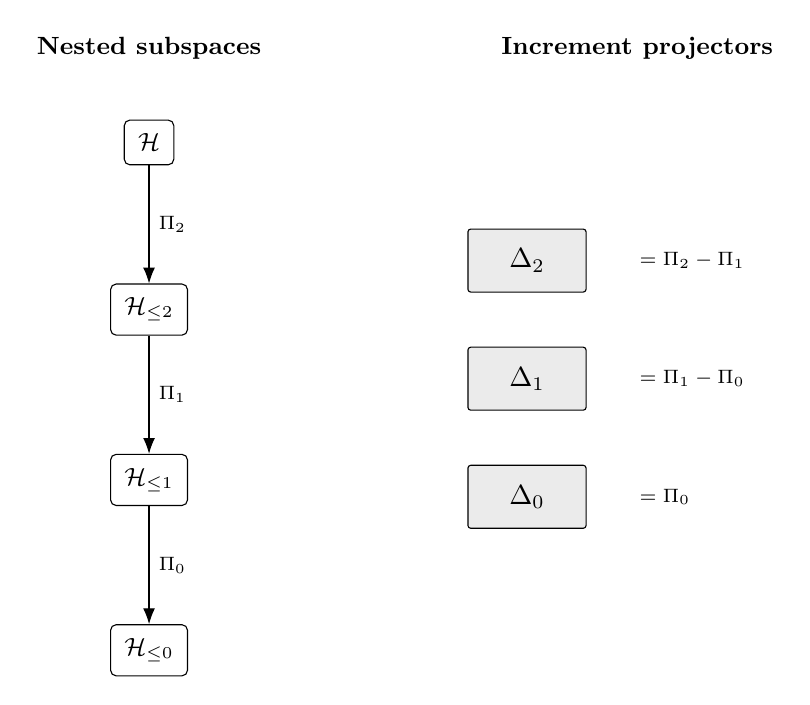
\begin{tikzpicture}[node distance=1.5cm]
  \node[font=\small\bfseries] at (0,1.2) {Nested subspaces};
  \node[font=\small\bfseries] at (6.2,1.2) {Increment projectors};

  \node[ccbox] (H) at (0,0) {$\cH$};
  \node[ccbox, below=of H] (H2) {$\CCHobs{2}$};
  \node[ccbox, below=of H2] (H1) {$\CCHobs{1}$};
  \node[ccbox, below=of H1] (H0) {$\CCHobs{0}$};

  \draw[ccarrow] (H) -- node[right, cclabel] {$\CCPi{2}$} (H2);
  \draw[ccarrow] (H2) -- node[right, cclabel] {$\CCPi{1}$} (H1);
  \draw[ccarrow] (H1) -- node[right, cclabel] {$\CCPi{0}$} (H0);

  \node[ccband, minimum width=1.5cm, minimum height=0.8cm] (D2) at (4.8,-1.5) {$\CCDelta{2}$};
  \node[ccband, minimum width=1.5cm, minimum height=0.8cm] (D1) at (4.8,-3.0) {$\CCDelta{1}$};
  \node[ccband, minimum width=1.5cm, minimum height=0.8cm] (D0) at (4.8,-4.5) {$\CCDelta{0}$};

  \node[right=0.55cm of D2, font=\scriptsize] {$= \CCPi{2} - \CCPi{1}$};
  \node[right=0.55cm of D1, font=\scriptsize] {$= \CCPi{1} - \CCPi{0}$};
  \node[right=0.55cm of D0, font=\scriptsize] {$= \CCPi{0}$};
\end{tikzpicture}%
}
\caption{Horizon tower with nested subspaces (left) and increment projectors as ``bands'' (right).}
\label{fig:horizon-tower}
\end{figure}

% --- Defect Round-Trip Diagram ---
\begin{figure}[ht]
\centering
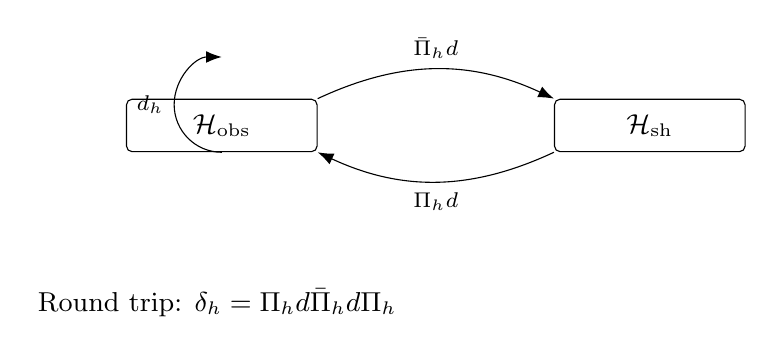
\begin{tikzpicture}[node distance=3cm, scale=1.1, every node/.style={scale=1.1}]
  % Observable and shadow
  \node[ccbox, minimum width=2.2cm] (obs) {$\cH_{\mathrm{obs}}$};
  \node[ccbox, minimum width=2.2cm, right=of obs] (sh) {$\cH_{\mathrm{sh}}$};

  % Arrows forming round trip
  \draw[ccarrow, bend left=25] (obs.north east) to node[above, cclabel] {$\CCPibar{h} d$} (sh.north west);
  \draw[ccarrow, bend left=25] (sh.south west) to node[below, cclabel] {$\CCPi{h} d$} (obs.south east);

  % Self-loop for observed operator
  \draw[ccarrow] (obs.south) arc[start angle=-90, end angle=-270, radius=0.55cm]
    node[left, pos=0.5, cclabel] {$\CCObs{d}{h}$};

  % Annotation
  \node[below=1.6cm of obs, font=\small, align=center] {
    Round trip: $\CCDefect{d}{h} = \CCPi{h} d \CCPibar{h} d \CCPi{h}$
  };
\end{tikzpicture}
\caption{Defect as ``round trip through shadow'': leakage out ($\CCPibar{h} d$) and return ($\CCPi{h} d$).}
\label{fig:defect-roundtrip}
\end{figure}

% ============================================================
\section{Positioning and Connections}
\label{sec:positioning}\lean{CoherenceCalculus.operatorCompression_eq_blockPP, CoherenceCalculus.unifiedGrammar_projection_algebra, CoherenceCalculus.towerCalculus_summary}
% ============================================================

This section situates Coherence Calculus relative to established mathematical
frameworks. Its ingredients are elementary: projection algebra, block
decomposition, and Hilbert-complex methods. It separates
standard background from the organizing contribution of the calculus.

\subsection{Finite observability in ergodic and systems settings}
\label{subsec:finite-observability-context}

The phrase \emph{finite observability} already has established narrow meanings
in nearby literatures. In ergodic theory, Ornstein and Weiss use it for
invariants that can be recovered almost surely from longer but still finite
typical observation windows, and show that entropy is the only finitely
observable invariant of stationary ergodic finite-valued processes in that
sense \cite{OrnsteinWeiss2007}. In linear systems theory, Kalman's
state-space framework and its descendants make observability precise by asking
which internal degrees of freedom are recoverable from finite output data
\cite{Kalman1963,Antoulas2005}. Coherence Calculus does not identify with
either framework, but it lives in the same conceptual neighborhood: the
observable/shadow split is treated as structural data rather than as a mere
numerical approximation device.

\subsection{Operator compression and projection-induced error}
\label{subsec:operator-compression}\lean{CoherenceCalculus.operatorCompression_eq_blockPP, CoherenceCalculus.leakageCorrectionTerm}

The basic operation of Coherence Calculus, namely compressing an operator $A$
to $\CCRestr{A}{h} = \CCPi{h} A \CCPi{h}$, is standard in numerical linear
algebra and model reduction.
Projection-based compression and the resulting coarse/fine correction terms are
standard in reduced-order modeling, multilevel solvers, and open-system
effective dynamics \cite{Antoulas2005,BriggsHensonMcCormick2000,BreuerPetruccione2002}.
The ``leakage correction'' $\CCLeakCorr{h}{A}{B} = \CCPi{h} A \CCPibar{h} B \CCPi{h}$ that appears in product compression is the same cross-term that arises in:
\begin{itemize}[itemsep=0.2em]
\item \textbf{Reduced-order modeling:} Galerkin projection onto a subspace introduces closure terms from the neglected modes.
\item \textbf{Multigrid and domain decomposition:} Coarse-grid corrections require accounting for fine-grid residuals.
\item \textbf{Quantum open systems:} Tracing over environment degrees of freedom generates effective dynamics with ``system-bath'' correction terms.
\end{itemize}
Coherence Calculus organizes these correction terms into a common grammar of
chain rules, product rules, and elimination patterns, rather than treating
each application separately.

\subsection{Conditional expectation and coarse-graining}
\label{subsec:coarse-graining}\lean{CoherenceCalculus.shadow_plus_proj_identity, CoherenceCalculus.proj_shadow_orthogonal}

When $\CCPi{h}$ is a conditional expectation (e.g., block averaging), the coherence defect $\CCTau{h}{F}{x} = \CCPi{h} F(x) - F(\CCPi{h} x)$ is the ``closure term'' familiar from:
\begin{itemize}[itemsep=0.2em]
\item \textbf{Turbulence modeling:} Reynolds decomposition and subgrid-scale closures.
\item \textbf{Statistical mechanics:} Coarse-grained free energies and renormalization group.
\item \textbf{Large eddy simulation:} Filtered equations require modeling of unresolved scales.
\end{itemize}
These interpretations are standard in coarse-grained fluid and statistical
descriptions \cite{Pope2000,Goldenfeld1992}.
The bilinear defect $\CCTauBi{h}{B}{x}{y}$
(Proposition~\ref{prop:product-rule}) is the same algebraic object that
appears as subgrid stress or eddy-viscosity defect in these settings.
Coherence Calculus does not solve the closure problem; it records exact
identities for the defect structure. The broader idea that elimination of
unresolved variables produces memory, noise, and effective closure terms is
also classical in the Mori--Zwanzig and optimal-prediction literature
\cite{Zwanzig1961,Mori1965,ChorinHaldKupferman2000}.

\subsection{Schur complement and Feshbach projection}
\label{subsec:schur-feshbach}\lean{schurComplement, effectiveOp, schur_factorization}

The Schur complement formula (Section~\ref{sec:resolvent-defect}) is classical
\cite{Haynsworth1968,Zhang2005}:
\[
(M/D) = A - BD^{-1}C \quad \text{for } M = \begin{pmatrix} A & B \\ C & D \end{pmatrix}.
\]
In physics, this is known as the \emph{Feshbach projection} or \emph{effective Hamiltonian} method
\cite{Feshbach1958,Feshbach1962}:
\begin{itemize}[itemsep=0.2em]
\item \textbf{Quantum mechanics:} Projecting onto a ``P-space'' generates an effective operator with ``self-energy'' corrections from the ``Q-space.''
\item \textbf{Scattering theory:} T-matrix formulations via elimination of closed channels.
\item \textbf{Renormalization:} Integrating out high-energy modes generates effective low-energy couplings.
\item \textbf{Statistical coarse-graining:} Projection formalisms generate exact memory and return terms for unresolved variables \cite{Zwanzig1961,Mori1965,ChorinHaldKupferman2000}.
\end{itemize}
Coherence Calculus uses the Schur complement as the canonical elimination
pattern for shadow degrees of freedom. The distinctive step is its systematic
connection to the tower calculus through derivative, antiderivative, and
telescoping identities.

\subsection{Multiresolution and nested projections}
\label{subsec:multiresolution}\lean{CoherenceCalculus.multiresolution_nesting, CoherenceCalculus.wavelet_detail_analog, CoherenceCalculus.increment_orthogonality}

The horizon tower $\CCPi{0} \le \CCPi{1} \le \cdots$ is a nested sequence of orthogonal projections.
This structure appears in:
\begin{itemize}[itemsep=0.2em]
\item \textbf{Wavelet analysis:} Multiresolution analysis with nested approximation spaces $V_0 \subset V_1 \subset \cdots$.
\item \textbf{Martingale theory:} Filtrations and conditional expectations with respect to nested $\sigma$-algebras.
\item \textbf{Spectral theory:} Spectral projections $E_{(-\infty, \lambda]}$ for self-adjoint operators.
\end{itemize}
Standard references include multiresolution analysis, martingale filtrations,
and spectral projection theory \cite{Mallat1989,Daubechies1992,Doob1953,ReedSimon1972}.
The tower derivative $\CCDer{A} = [\CCIndexOp, A]$ and antiderivative
$\CCInt{B}$ provide algebraic tools for these nested structures. The
fundamental theorem (Theorem~\ref{thm:ftc-tower}) is an operator analogue of a
reconstruction formula.

\subsection{Hilbert complexes and Hodge theory}
\label{subsec:hodge}\lean{CoherenceCalculus.complex_nilpotency, CoherenceCalculus.intertwining_preserves_complex, CoherenceCalculus.cohomology_splits}

The solver layer (Section~\ref{subsec:solver-layer}) uses standard finite-dimensional Hodge theory
\cite{ArnoldFalkWinther2006,Schwarz1995,Warner1983}:
\begin{itemize}[itemsep=0.2em]
\item \textbf{Hodge decomposition:} $H^k = \Img(D_{k-1}) \oplus \Img(D_k^*) \oplus \Ker(\mathcal{L}_k)$ is the standard orthogonal decomposition.
\item \textbf{Green operator:} $\CCGreen{k} = \mathcal{L}_k^{-1}$ under exactness is the standard pseudo-inverse.
\item \textbf{Homotopy identity:} $DK + KD = I$ under exactness is the standard Hodge--de Rham result.
\end{itemize}
For infinite-dimensional Hilbert complexes, the same circle of ideas extends to
functional-analytic Hilbert-complex settings and finite element exterior
calculus \cite{ArnoldFalkWinther2006}.
Coherence Calculus restricts to the finite-dimensional case at the structural
level. Infinite-dimensional extensions require the usual functional-analytic
care with closedness and Fredholm conditions.

\subsection{Distinctive Features}
\label{subsec:what-is-new}\lean{CoherenceCalculus.unifiedGrammar_projection_algebra, CoherenceCalculus.towerCalculus_summary, CoherenceCalculus.diagonal_offdiagonal_decomposition}

The individual components above are standard. In the present setting, the
distinctive features are:
\begin{enumerate}[label=(\roman*), itemsep=0.3em]
\item \textbf{Unified grammar:} Chain rule, product rule, and elimination patterns organized around the defect identity.
\item \textbf{Tower calculus:} Derivative $\partial = [\CCIndexOp, \cdot]$, antiderivative $\CCInt{\cdot}$, fundamental theorem, and IBP as a self-contained calculus on operator algebras.
\item \textbf{Completion-and-selection algebra:} Systematic reduction of locality, symmetry, and conservation constraints to explicit operator selections via isotypic decomposition.
\item \textbf{Integration of solver layer:} Hodge/Green/homotopy operators connected to the tower structure, with holographic saturation as relative exactness.
\end{enumerate}

% ============================================================
\section{Operator Interface: Additive Horizon Systems}
\label{sec:bedrock}
% ============================================================

This section isolates the interface on which the structural calculus depends.
Only the algebraic and energetic data needed for projection identities, defect
identities, tower calculus, elimination, and solver constructions are fixed
here. No preferred coordinate model and no counting realization are imposed at
this stage.

% ------------------------------------------------------------
\subsection{Additive state spaces and energy}
\label{subsec:algebraic-foundations}
% ------------------------------------------------------------

\begin{definition}[Additive state space]\label{def:vector-space}\lean{AdditiveStateSpace}
An \emph{additive state space} is a set $\cH$ equipped with operations
\[
0 \in \cH,
\qquad
+ : \cH \times \cH \to \cH,
\qquad
- : \cH \to \cH,
\]
such that for all $x,y,z \in \cH$,
\begin{enumerate}[label=(\roman*), itemsep=0.2em]
\item $(x+y)+z = x+(y+z)$,
\item $x+y = y+x$,
\item $x+0 = x$,
\item $x+(-x)=0$.
\end{enumerate}
\end{definition}

\begin{definition}[Energy pairing]\label{def:inner-product}\lean{EnergyPairing}
An \emph{energy pairing} on an additive state space $\cH$ is a symmetric
positive bilinear form
\[
\langle \cdot,\cdot\rangle : \cH \times \cH \to \bbR
\]
such that
\[
\langle x,x\rangle \ge 0
\qquad\text{for all }x\in\cH,
\]
and $\langle x,x\rangle = 0$ only when $x=0$.
The induced energy norm is
\[
\|x\|^2 := \langle x,x\rangle.
\]
\end{definition}

\begin{definition}[Finite coherence space]\label{def:hilbert-space}\lean{FiniteCoherenceSpace}
A \emph{finite coherence space} is an additive state space equipped with an
energy pairing. Whenever orthogonality, adjoints, or defect energies are used
in later chapters, they are understood relative to that fixed pairing.
\end{definition}

% ------------------------------------------------------------
\subsection{Horizon towers and observed operators}

\begin{definition}[Horizon tower]
\label{def:horizon-tower}\lean{HorizonTower}
A \emph{horizon tower} on $\cH$ is a nested family of idempotent observable
projections $(\CCPi{h})_{h\in\bbN}$.
Nestedness means that coarse observation after finer observation changes
nothing:
\[
\CCPi{h}\CCPi{h'}=\CCPi{h}
\qquad (h\le h').
\]
\end{definition}

\begin{definition}[Shadow projector]\label{def:shadow-projector}\lean{shadowProj}
The shadow at horizon $h$ is the complementary operator
\[
\CCPibar{h}:=\id-\CCPi{h}.
\]
Thus every state splits into visible part plus shadow:
\[
x=\CCPi{h}x+\CCPibar{h}x.
\]
\end{definition}

\begin{definition}[Transitivity of horizons]\label{def:transitivity}\lean{nested_proj_comp}\lean{nested_proj_comp_ge}
For a nested horizon tower,
\[
\CCPi{h}\CCPi{h'}=\CCPi{h}
\qquad (h\le h'),
\qquad
\CCPi{h'}\CCPi{h}=\CCPi{h}
\qquad (h\le h').
\]
This is the algebraic coherence law for observation across different
resolutions.
\end{definition}

\begin{definition}[Energy-orthogonal tower]\label{def:orthogonal-tower}\lean{EnergyOrthogonalTower}
Let $\cH$ carry an energy pairing. A horizon tower is
\emph{energy-orthogonal} if each projection $\CCPi{h}$ is self-adjoint for that
pairing and
\[
\langle \CCPi{h}x,\CCPibar{h}y\rangle = 0
\qquad
\text{for all }x,y\in\cH.
\]
Equivalently, each horizon cut splits the state space into an orthogonal
observable sector and an orthogonal shadow sector.
\end{definition}

\begin{definition}[Additive operator]\label{def:linear-operator}\lean{AddMap}
An \emph{additive operator} on $\cH$ is a map $A:\cH\to\cH$ preserving addition
and zero:
\[
A(x+y)=Ax+Ay,
\qquad
A(0)=0.
\]
\end{definition}

\begin{definition}[Energy adjoint]\label{def:adjoint}\lean{HasEnergyAdjoint}\lean{defectEnergy_operator_form}
Given additive operators $A$ and $A^\ast$, one says that $A^\ast$ is an
\emph{energy adjoint} of $A$ if
\[
\langle Ax,y\rangle = \langle x,A^\ast y\rangle
\qquad
\text{for all }x,y\in\cH.
\]
This is exactly the adjoint structure needed for the operator form of defect
energy.
\end{definition}

\begin{definition}[Graded differential and nilpotency]
\label{def:nilpotent-differential}\lean{isNilpotent}
A \emph{nilpotent differential} on $\cH$ is an additive operator $d$ satisfying
\[
d^2=0.
\]
\end{definition}

\begin{definition}[Observed operator]
\label{def:observed-operator}\lean{observedOp}
Given a horizon tower and an additive operator $A$, the observed operator at
horizon $h$ is
\[
\CCObs{A}{h}:=\CCPi{h}A\CCPi{h}.
\]
\end{definition}

\begin{definition}[Leakage operator]
\label{def:leakage-operator}\lean{leakageOp}
The leakage operator is
\[
\CCLeak{A}{h}:=\CCPibar{h}A\CCPi{h}.
\]
It measures what leaves the observable sector when $A$ acts on visible input.
\end{definition}

\begin{definition}[Return operator]
\label{def:return-operator}\lean{returnOp}
The return operator is
\[
R_h:=\CCPi{h}A\CCPibar{h}.
\]
It measures what returns from shadow to the observable sector.
\end{definition}

\begin{remark}[Defect as round trip]
\label{rem:defect-round-trip}\lean{defect_factorization}
The defect is the observable round trip through shadow:
\[
\CCDefect{A}{h}=R_h\,\CCLeak{A}{h}
=\CCPi{h}A\CCPibar{h}A\CCPi{h}.
\]
Leakage and defect are therefore different objects. Leakage is escape;
defect is returned nonclosure.
\end{remark}

\paragraph{Interface principle.}
The structural theorems of Part~II depend only on the data above together with
the additional hypotheses stated locally in each chapter. No coordinate
realization, counting model, or physical interpretation is used at this stage.

\paragraph{Realizations enter later.}
Part~I proves that Closure Balance supplies a distinguished finite
realization of this interface. Chapter~13 proves that conservative
characteristic transport can furnish another realization. Both belong to the
realized-model layer, not to the structural interface itself.

% ============================================================
\section{Foundational Proof Patterns}
\label{sec:foundational-lemmas}
% ============================================================

This section records the proof patterns used repeatedly in the clean horizon calculus.
They isolate the resolution split, the block decomposition, the telescoping identity, and the Pythagorean split that drive the later arguments.

% ------------------------------------------------------------
\subsection{Resolution-of-Identity Expansion}
\label{subsec:resolution-lemma}
% ------------------------------------------------------------

The basic split behind the calculus is the observable/shadow decomposition at a fixed horizon.

\begin{lemma}[Resolution-of-Identity Expansion]
\label{lem:resolution-identity}\lean{resolution_of_identity}
Let $\CCPi{h}$ be a horizon projection with shadow $\CCPibar{h} = I - \CCPi{h}$.
For any state $x$,
\[
x = \CCPi{h}x + \CCPibar{h}x.
\]
\end{lemma}

\begin{proof}
By definition, $\CCPibar{h}x = x - \CCPi{h}x$.
Hence
\[
\CCPi{h}x + \CCPibar{h}x = \CCPi{h}x + (x - \CCPi{h}x) = x.
\]
\end{proof}

\paragraph{Usage pattern.}
Whenever a proof says ``insert the horizon split,'' it means: replace a state
by its observable part plus its shadow part and then distribute.

% ------------------------------------------------------------
\subsection{Block Splitting Lemma}
\label{subsec:block-splitting}
% ------------------------------------------------------------

\begin{lemma}[Block Splitting for Operator Products]
\label{lem:block-splitting}\lean{block_splitting}
For additive operators $A, B$ and horizon projection $\CCPi{h}$,
\[
\CCRestr{(AB)}{h} = \CCObs{A}{h}\CCObs{B}{h} + \CCLeakCorr{h}{A}{B},
\]
where
\[
\CCLeakCorr{h}{A}{B} := \CCPi{h} A \CCPibar{h} B \CCPi{h}.
\]
\end{lemma}

(Proof in Appendix~\ref{sec:appendix-tower}.)

% ------------------------------------------------------------
\subsection{Three-Level Telescope}
\label{subsec:telescoping-lemma}
% ------------------------------------------------------------

\begin{lemma}[Three-Level Telescope]
\label{lem:orthogonal-telescoping}\lean{telescope_3_terms}
Let $(\CCPi{h})_{h \in \bbN}$ be a transitive horizon tower.
For horizons $h_0 \le h_1 \le h_2$ and any $x \in \cH$,
\[
(\CCPi{h_1} - \CCPi{h_0})x
+
\Bigl((\CCPi{h_2} - \CCPi{h_1})x + (x - \CCPi{h_2}x)\Bigr)
=
x - \CCPi{h_0}x.
\]
\end{lemma}

\begin{proof}
This is a direct telescoping regrouping:
\[
x - \CCPi{h_0}x
=
(\CCPi{h_1}x - \CCPi{h_0}x) + (\CCPi{h_2}x - \CCPi{h_1}x) + (x - \CCPi{h_2}x).
\]
The intermediate horizon contributions cancel.
\end{proof}

\paragraph{Calculus interpretation.}
This is the algebraic core of HFT-2: adjacent refinement layers close
internally, so only the outer remainder survives.

% ------------------------------------------------------------
\subsection{Pythagorean Norm Splitting}
\label{subsec:pythagorean-norm}
% ------------------------------------------------------------

\begin{lemma}[Pythagorean Norm Splitting]
\label{lem:pythagorean-splitting}\lean{pythagorean_splitting}\lean{pythagorean_splitting_observed}\lean{defectEnergy}
Assume the horizon tower is energy-orthogonal.
Then:
\begin{enumerate}[label=(\roman*)]
\item \textbf{State splitting:} for any $x \in \cH$,
\[
\|x\|^2 = \|\CCPi{h} x\|^2 + \|\CCPibar{h} x\|^2.
\]
\item \textbf{Operator action splitting:} for a closure operator $d$ and $x \in \CCHobs{h}$,
\[
\|dx\|^2 = \|\CCObs{d}{h} x\|^2 + \CCDefEnergy{h}{x},
\]
where
\[
\CCDefEnergy{h}{x} := \|\CCLeakExpr{d}{h}x\|^2.
\]
\end{enumerate}
\end{lemma}

\begin{proof}
(i) This is the exact energy decomposition at the horizon cut.

(ii) Apply (i) to $dx$.
If $x \in \CCHobs{h}$, then $\CCPi{h}x = x$, so the observable and shadow pieces of $dx$ are exactly $\CCObs{d}{h}x$ and $\CCLeakExpr{d}{h}x$.
\end{proof}

\begin{quote}\small
\textbf{Intuition.}
The horizon split does not create or destroy energy.
It partitions it into what is already visible and what remains in shadow.
\end{quote}

% ============================================================
\section{The Horizon Fundamental Theorem}
\label{sec:hft}
% ============================================================

This section records the structural projection laws behind the calculus.
The order matters:

\begin{enumerate}[label=(\roman*)]
\item for any square-zero additive operator, projection produces an exact defect identity;
\item for any compatible horizon tower, orthogonal refinement produces an exact telescoping law in energy;
\item realized models of the calculus may then instantiate these structural laws with canonical concrete data.
\end{enumerate}

The canonical closure-balance realization of these laws is deferred to
Part~I. This chapter develops only the structural theorem layer.

\begin{theorem}[General HFT-1]
\label{thm:HFT1-general}\lean{HFT1_general_nilpotent}
Let $\cH$ be an additive state space with a transitive horizon tower $(\CCPi{h})_{h\in\bbN}$, let $A$ be an additive operator on $\cH$, and assume
\[
A^2 = 0.
\]
Define the observed operator $\CCObs{A}{h} := \CCPi{h} A \CCPi{h}$ and $\CCPibar{h} := I - \CCPi{h}$.
Then
\[
\CCObs{A}{h}^2 \;=\; -\,\CCPi{h} A \CCPibar{h} A \CCPi{h}.
\]
Equivalently,
\[
\CCObs{A}{h}^2 \;=\; -\,\CCDefectExpr{A}{h}.
\]
\end{theorem}

\begin{proof}
Compute
\[
0 = \CCPi{h} A^2 \CCPi{h}
= \CCPi{h} A(\CCPi{h} + \CCPibar{h})A\CCPi{h}
= \underbrace{\CCPi{h} A\CCPi{h} A\CCPi{h}}_{\CCObs{A}{h}^2} + \CCPi{h} A \CCPibar{h} A \CCPi{h}.
\]
Rearranging gives the claim.
\end{proof}

The remaining part of the Horizon Fundamental Theorem is the refinement law.
Its algebraic content is that adjacent refinement layers close internally and telescope.
Its metric content is that, when those layers are orthogonal, the hidden remainder decomposes into an exact sum of layer energies.

\begin{theorem}[General HFT-2]
\label{thm:HFT2-general}\label{thm:HFT}\lean{HFT2_finite_energy}\lean{HFT2_faithful_stabilized}
Let $(\CCPi{h})_{h\in\bbN}$ be a nested horizon tower on $\cH$ whose refinement layers split orthogonally, so that each horizon cut satisfies an exact Pythagorean decomposition.
For nested horizons $h_0 \le h_1 \le \cdots \le h_N$ and any $x\in\cH$,
\[
\|x - \CCPi{h_0} x\|^2
=
\sum_{j=0}^{N-1} \|(\CCPi{h_{j+1}} - \CCPi{h_j})x\|^2 + \|x - \CCPi{h_N} x\|^2.
\]
If the tower is \emph{tail-faithful in the HFT-2 sense}, meaning that the tail
energy eventually vanishes along consecutive refinement, then there exists $N$
such that for every $k \ge 0$,
\[
\|x - \CCPi{h_0} x\|^2
=
\sum_{j=0}^{N+k-1} \|(\CCPi{h_0+j+1} - \CCPi{h_0+j})x\|^2.
\]
\end{theorem}

\begin{proof}
The finite statement is the orthogonal telescoping law for the refinement chain: adjacent internal interfaces cancel algebraically, and orthogonality converts that telescoping decomposition into an exact sum of energies.
The tail-faithful statement is the exact discrete stabilization of those finite
prefix sums once the tail energy vanishes.
No analytic infinite-series machinery is used at this stage.
\end{proof}

\begin{remark}[HFT-2 as realized exactification ledger]
\label{rem:hft2-realized-exactification-ledger}\lean{CoherenceCalculus.TerminationData, CoherenceCalculus.nonterminal_incidences_continue, CoherenceCalculus.pair_telescope_energy}
At the bedrock level, the termination law identifies zero defect with
terminality, while nonterminal incidence continues by strict extension and
closure defect can vanish only on strict extension if terminality is
eventually reached
(Axioms~\ref{ax:termination} and~\ref{ax:nonretroactive-exactification}).
HFT-2 is the first realized telescoping law for that continuation burden:
adjacent refinement layers cancel internally, and the remaining quantity is an
exact sum of realized layer energies. In this sense HFT-2 does not generate
continuation; it measures the additive burden of exactification once a horizon
tower has been chosen.
\end{remark}

\begin{remark}[Tail faithfulness versus continuum-bridge faithfulness]
\label{rem:hft2-tail-faithfulness}
\lean{HFT2_faithful_prefix_exact, HFT2_faithful_stabilized}
The HFT-2 use of ``tail-faithful'' is a finite-stabilization condition: after
some finite refinement stage, the hidden tail energy vanishes exactly.
This is stronger than, and distinct from, the continuum-bridge notion of
faithfulness as strong limit recovery along an infinite tower.
\end{remark}

\begin{lemma}[One-step shadow-energy split]
\label{lem:hft2-one-step}\lean{pair_telescope_energy}
Under the hypotheses of Theorem~\ref{thm:HFT2-general}, every nested pair of horizons $h_0 \le h_1$ satisfies
\[
\|x - \CCPi{h_0} x\|^2
=
\|(\CCPi{h_1} - \CCPi{h_0})x\|^2 + \|x - \CCPi{h_1} x\|^2.
\]
\end{lemma}

\begin{proof}
Split the $h_0$-shadow into the part revealed at horizon $h_1$ and the remaining $h_1$-shadow.
Orthogonality of the refinement split gives the exact Pythagorean identity.
\end{proof}

\begin{corollary}[Three-level HFT-2]
\label{cor:hft2-three-level}\lean{HFT2_three_level_energy}
Under the hypotheses of Theorem~\ref{thm:HFT2-general}, every triple $h_0 \le h_1 \le h_2$ satisfies
\[
\|x - \CCPi{h_0} x\|^2
=
\|(\CCPi{h_1} - \CCPi{h_0})x\|^2
+ \|(\CCPi{h_2} - \CCPi{h_1})x\|^2
+ \|x - \CCPi{h_2} x\|^2.
\]
\end{corollary}

\begin{proof}
Apply Lemma~\ref{lem:hft2-one-step} first to $(h_0,h_1)$ and then to $(h_1,h_2)$.
\end{proof}

\begin{proposition}[Faithful exact-prefix capture]
\label{prop:hft2-prefix-exact}\lean{HFT2_faithful_prefix_exact}
If the tower is tail-faithful in the sense of
Theorem~\ref{thm:HFT2-general}, then for every initial horizon $h_0$ there
exists a finite stage $N$ such that
\[
\|x - \CCPi{h_0} x\|^2
=
\sum_{j=0}^{N-1} \|(\CCPi{h_0+j+1} - \CCPi{h_0+j})x\|^2.
\]
So the total hidden energy is already captured by a finite prefix of consecutive refinement increments.
\end{proposition}

\begin{proof}
By tail faithfulness, the tail energy vanishes after sufficiently many
consecutive refinements.
At that stage the finite telescoping identity has zero remainder, so only the prefix sum remains.
\end{proof}

\begin{proposition}[Structured infinite choice along a refinement tower]
\label{prop:structured-infinite-choice}\lean{RootedFiniteRefinementTower}\lean{structured_infinite_choice}
Let $(X_n)_{n\in\bbN}$ be a rooted refinement tower with predecessor maps
\[
p_n : X_{n+1} \to X_n,
\]
such that:
\begin{enumerate}[label=(\roman*),itemsep=0.2em]
\item the initial stage $X_0$ is given by an explicit nonempty finite list of roots;
\item for each $x \in X_n$, the refinement fiber above $x$ is given by an explicit nonempty finite list;
\item every listed refinement projects back to its parent under $p_n$.
\end{enumerate}
Then there exists a coherent infinite thread $(x_n)_{n\in\bbN}$ with
\[
x_n \in X_n,
\qquad
p_n(x_{n+1}) = x_n
\quad\text{for all }n.
\]
The construction is explicit: choose the first root, then choose the first listed refinement above it at every stage.
\end{proposition}

\begin{proof}
Start from the first listed root in $X_0$. Given $x_n$, take the first listed refinement above it and call that $x_{n+1}$. By hypothesis each refinement fiber is nonempty, so the recursion never stops, and by hypothesis each chosen refinement projects back to its parent. This gives an infinite coherent thread.
\end{proof}

\begin{quote}\small
\textbf{Scope.} This is not the full Axiom of Choice. It is a constructive infinite-choice principle for explicitly finite refinement systems. Its role here is to show how the finite tower grammar already supports coherent infinite selection in the structured limit.
\end{quote}

\begin{corollary}[Countable structured choice from finite partial choices]
\label{cor:countable-structured-choice}\lean{ExplicitFiniteFamily}\lean{countable_structured_choice}
Let $(F_n)_{n\in\bbN}$ be a countable family of explicitly finite nonempty fibers. For each finite stage $n$, let a \emph{partial choice} mean a compatible choice on the first $n$ fibers. Then there exists:
\begin{enumerate}[label=(\roman*),itemsep=0.2em]
\item a global sequence $(c_n)_{n\in\bbN}$ with $c_n \in F_n$ for every $n$;
\item a coherent chain of partial choices whose $(n+1)$st stage is obtained from its $n$th stage by adjoining $c_n$.
\end{enumerate}
\end{corollary}

\begin{proof}
The stage-$n$ partial choices form a rooted finite refinement tower: the predecessor map drops the last coordinate, and every stage extends by choosing one element from the next explicit finite fiber. Proposition~\ref{prop:structured-infinite-choice} therefore yields a coherent infinite thread of partial choices. Reading the new coordinate at each stage gives the global sequence $(c_n)$.
\end{proof}

\subsection{Dyadic refinement bridge}

The constructive refinement principles above already support a first continuum-like layer without importing reals, quotients, or field structure.
The bridge is explicit and dyadic: binary choices build a tower of adjacent endpoint data on finer and finer unit meshes.

\begin{proposition}[Finite dyadic address injectivity]\label{prop:dyadic-address-injective}\lean{partialChoice_snoc_eq_iff}\lean{refineDyadicCell_eq_iff}
Extending a finite dyadic address by one more binary digit is injective in both pieces of explicit data.
Equivalently, if two one-step refinements agree, then their parent addresses agree and their final digits agree.
\end{proposition}

\begin{proof}
At the finite level, a dyadic address is built by adjoining one last binary digit to a shorter address.
So equality of two refined addresses forces equality of the shorter addresses and equality of the final digits separately.
\end{proof}

\begin{proposition}[Dyadic interval refinement]\label{prop:dyadic-refinement}\lean{dyadicCell_two_children}\lean{child_intervals_distinct}\lean{intervalsOfDigits_leftIndex_step}\lean{intervalsOfDigits_rightIndex_step}\lean{intervalsOfDigits_mesh}
At depth $n$, binary refinement determines dyadic interval data with adjacent endpoint indices $(\ell_n,r_n)$ satisfying
\[
r_n = \ell_n + 1,
\qquad
r_n \le 2^n.
\]
Each stage has exactly two distinct children.
If the next digit is left, then
\[
\ell_{n+1} = 2\ell_n,
\qquad
r_{n+1} = 2\ell_n + 1.
\]
If the next digit is right, then
\[
\ell_{n+1} = 2\ell_n + 1,
\qquad
r_{n+1} = 2r_n.
\]
\end{proposition}

\begin{proof}
This is the direct recursion of binary refinement.
Left refinement takes the left half of the current dyadic cell, while right refinement takes the right half; the endpoint formulas are exactly the resulting doubled-index updates on the finer mesh.
\end{proof}

\begin{proposition}[Binary threads yield dyadic point-candidates]\label{prop:dyadic-point-candidates}\lean{binarySequence_exists}\lean{unitPointOfDigits}\lean{leftUnitPoint}\lean{intervalsOfDigits_nested_scaled}\lean{unitPoint_mesh_strict}
Every infinite binary digit sequence determines a coherent dyadic interval thread on the unit mesh.
At each step, the next interval is nested inside the previous one after passing to the common finer denominator, and the mesh strictly refines from $2^n$ to $2^{n+1}$.
Hence the present structural layer already supports quotient-free dyadic
unit-point candidates.
\end{proposition}

\begin{proof}
Read each digit as a left/right child choice in the binary refinement tower.
The resulting endpoint recursion gives a coherent nested interval thread, and the denominator doubles at every step.
Taking the constant-left sequence gives a canonical example.
\end{proof}

\begin{quote}\small
\textbf{Scope.} This is still a pre-real layer.
Ambiguous binary tails have not yet been identified, so no quotient of equivalent dyadic expansions is taken here.
The present structural layer already forces a rigorous shrinking-thread
scaffold above the discrete level.
\end{quote}

\begin{quote}\small
\textbf{Intuition (HFT-1).} The full boundary closes: $d^2=0$ on the uncropped coherence space. But the \emph{observed} boundary $\CCObs{d}{h}$ is the cut $\CCPi{h} d \CCPi{h}$, and that cut need not close. The failure is exactly the ``round trip through the shadow'': apply $d$, some escapes to the shadow, apply $d$ again, some returns. That returned part is the defect.
\end{quote}

\begin{quote}\small
\textbf{Intuition (HFT-2).} The total ``distance'' from $x$ to its coarsest projection decomposes into orthogonal increments at each refinement level. This is the Pythagorean theorem applied to a tower of nested subspaces, with integration expressed as a sum of layer-by-layer contributions.
\end{quote}

\begin{tcolorbox}[colback=yellow!5, colframe=black!70, title={Warning: Zero defect $\neq$ conservation}]
\label{box:zero-defect-warning}\lean{returnOp}\lean{defect_factorization}
\textbf{The three operators.} For horizon projection $\CCPi{h}$ with $\CCPibar{h} = I - \CCPi{h}$:
\begin{align*}
L_h &:= \CCPibar{h} d \CCPi{h} &&\text{(leakage: observable $\to$ shadow)}, \\
R_h &:= \CCPi{h} d \CCPibar{h} &&\text{(return: shadow $\to$ observable)}, \\
\CCDefect{d}{h} &:= R_h L_h = \CCPi{h} d \CCPibar{h} d \CCPi{h} &&\text{(defect: round-trip)}.
\end{align*}

\textbf{Key distinctions:}
\begin{itemize}[itemsep=0.2em]
\item $\CCDefect{d}{h} = 0$ is \emph{algebraic closure} (a compositional identity), \textbf{not} metric conservation.
\item $L_h \neq 0$ with $\CCDefect{d}{h} = 0$ is possible when $R_h = 0$ (``silent leak'').
\item Orthogonality of $\CCPi{h}$ is what makes the defect energy $\|L_h x\|^2$ well-defined.
\end{itemize}
\end{tcolorbox}

\begin{lemma}[Silent leak configuration]
\label{lem:silent-leak}\lean{silent_leak_configuration}
There exist $\cH$, a projection $\Pi$, and $d$ with $d^2 = 0$ such that:
\begin{enumerate}[label=(\roman*),itemsep=0.1em]
\item $d_\Pi := \Pi d \Pi$ satisfies $d_\Pi^2 = 0$ (algebraic closure),
\item $L := (I - \Pi) d \Pi \neq 0$ (nonzero leakage),
\item $\delta := \Pi d (I - \Pi) d \Pi = 0$ (zero defect, because $R = \Pi d (I-\Pi) = 0$).
\end{enumerate}
\end{lemma}

(Proof in Appendix~\ref{sec:appendix-tower}.)

\subsection{Illustration: The 4-vertex path}

Returning to the running example (Example~\ref{ex:hello-world}): the
4-vertex path with block-averaging horizon. HFT-1 applies because the graded
differential $D$ satisfies $D_{k+1} \circ D_k = 0$
(Definition~\ref{def:nilpotent-differential}). The defect term is exactly the
within-block contribution that the coarse observer cannot represent. This
subsection remains illustrative; the theorem-bearing statements are the general
and coherence-realized HFT identities above.

\subsection{Defect operator and defect energy}

\begin{definition}[Defect operator]\label{def:defect-operator}\lean{defectOp}
Define the \emph{defect operator}
\[
\CCDefect{d}{h} := \CCDefectExpr{d}{h}
\quad\text{so that}\quad
\CCObs{d}{h}^2 = -\CCDefect{d}{h}.
\]
\end{definition}

\begin{definition}[Defect energy]\label{def:defect-energy-operator}\lean{defectEnergy}\lean{defectEnergy_operator_form}
Define the \emph{defect energy} on $\cH$ by
\[
\CCDefEnergy{h}{x} := \|\CCLeak{d}{h} x\|^2 = \|\CCLeakExpr{d}{h}\, x\|^2.
\]
Whenever the leakage map admits an energy adjoint $\CCLeak{d}{h}^\ast$ for the coordinate pairing of the state space, this can be written in operator form as
\[
\CCDefEnergy{h}{x} = \langle x, \CCDefOp{d}{h} x\rangle,
\qquad
\CCDefOp{d}{h} := \CCLeak{d}{h}^\ast \CCLeak{d}{h}.
\]
\end{definition}

\paragraph{Why this is a calculus.}
The defect $\CCDefect{d}{h}$ is the derivative object: it measures failure of
closure under observation. The telescoping identity (HFT-2) is the integration
analog: total deviation decomposes into orthogonal layer increments. Defect
energy $\CCDefEnergy{h}{x} = \|\CCLeak{d}{h} x\|^2$ quantifies the portion of
$dx$ that lands in the shadow and is therefore invisible at horizon $h$.

\paragraph{Interpretation note.}
\label{rem:interpretation-note}
The defect energy is an algebraic quantity measuring representational mismatch,
not physical loss. Finer horizons do not make defect energy monotone for
arbitrary states; that requires additional representability hypotheses, as made
explicit later in Proposition~\ref{prop:log-defect}. In a faithful tower, the
tail term in HFT-2 eventually vanishes after finite stabilization. No
thermodynamic or information-theoretic interpretation is claimed here without
additional structure.

The next section records chain and product rules for coherence defects under composition, analogous to the Leibniz and chain rules of classical calculus.

% ============================================================
\section{Tower Calculus}
\label{sec:tower-calculus}
% ============================================================

The defect identities of Chapter~5 admit a companion calculus on operators
adapted to a discrete horizon tower. This calculus is not introduced as new
analysis. It is a clean way to record cross-scale transport, reconstruction, and exact
telescoping on finite or finitely supported towers.

\subsection{Scale index and tower derivative}
\label{subsec:tower-derivative}

\begin{definition}[Scale index operator]
\label{def:scale-index-operator}\lean{towerIndexOperator}
Assume the horizon tower is split into refinement bands
\[
\Delta_h := \CCPi{h} - \CCPi{h-1},
\qquad
\CCPi{-1} := 0,
\]
so that the observable space is the orthogonal sum of its bands. The
\emph{scale index operator} $\CCIndexOp$ is the operator that acts by
multiplication by $h$ on the $h$th band:
\[
\CCIndexOp|_{\Delta_h \cH} = h\, I.
\]
\end{definition}

\begin{definition}[Tower derivative]
\label{def:tower-derivative}\lean{towerDerivative}
For an operator $A$ on a band-split horizon space, define its
\emph{tower derivative} by
\[
\CCDer{A} := \CCComm{\CCIndexOp}{A}.
\]
\end{definition}

\begin{lemma}[Block formula and Leibniz rule]
\label{lem:tower-derivative-block}\lean{towerDerivative_block_formula, towerDerivative_leibniz}
Let $\CCBlock{A}{h}{k} := \Delta_h A \Delta_k$ denote the $(h,k)$ block of $A$.
Then
\[
\CCBlock{\CCDer{A}}{h}{k} = (h-k)\, \CCBlock{A}{h}{k}.
\]
Consequently,
\[
\CCDer{(AB)} = \CCDer{A}\, B + A\, \CCDer{B}.
\]
\end{lemma}

(Proof in Appendix~\ref{sec:appendix-tower}.)

\subsection{Transport order on the tower}
\label{subsec:tower-transport-order}

\begin{definition}[Tower transport order]\lean{towerTransportOrderAtMost}
\label{def:tower-transport-order}
Let $(\CCPi{h})_{h\in\bbN}$ be an energy-orthogonal horizon tower with band
projectors $\CCDelta{h}=\CCPi{h}-\CCPi{h-1}$. An operator $A$ on $\cH$ has
\emph{tower transport order at most $m$} if
\[
\CCDelta{j}A\CCDelta{k}=0
\qquad\text{whenever }|j-k|>m.
\]
Equivalently, $A$ transports mass across at most $m$ horizon bands in one step.
If $m$ is the least such integer, it is called the \emph{tower transport order}
of $A$.
\end{definition}

\begin{proposition}[Order arithmetic on the tower]\lean{towerTransportOrder_add_certificate, towerTransportOrder_comp, towerTransportOrder_derivative}
\label{prop:tower-order-arithmetic}
Let $A$ and $B$ be operators on a band-split horizon tower.
\begin{enumerate}[label=(\roman*), leftmargin=2em, itemsep=0.2em]
\item If $A$ has order at most $m$ and $B$ has order at most $n$, then
      $A+B$ has order at most $\max\{m,n\}$.
\item If $A$ has order at most $m$ and $B$ has order at most $n$, then
      $AB$ has order at most $m+n$.
\item If $A$ has order at most $m$, then the tower derivative $\CCDer{A}$ has
      order at most $m$.
\end{enumerate}
\end{proposition}

(Proof in Appendix~\ref{sec:appendix-tower}.)

\subsection{Reversible transport and recursion}
\label{subsec:reversible-transport-recursion}

\begin{definition}[Sequence transport space]\lean{SequenceTransportSpace}
\label{def:sequence-transport-space}
Let $F$ be a Hilbert space. The \emph{sequence transport space} on $F$ is the
space
\[
F^{\bbZ}
\]
of bilateral sequences $x=(x_n)_{n\in\bbZ}$ with $x_n\in F$ for every
$n\in\bbZ$.
\end{definition}

\begin{definition}[Recursion operator induced by a transport base]\lean{transportRecursionOperator}
\label{def:transport-recursion-operator}
Let $B:F\to F$ be a bounded operator. The \emph{recursion operator} induced by
$B$ is the map
\[
\mathcal R_B:F^{\bbZ}\to F^{\bbZ}
\]
defined by
\[
(\mathcal R_B x)_n := x_{n+1} - Bx_n + x_{n-1}.
\]
\end{definition}

\begin{lemma}[Kernel characterization of the recursion operator]\lean{transport_recursion_kernel}
\label{lem:transport-recursion-kernel}
Let $B:F\to F$ be bounded. A sequence $x=(x_n)_{n\in\bbZ}$ satisfies
\[
\mathcal R_Bx=0
\]
if and only if it obeys the second-order recurrence
\[
x_{n+1}=Bx_n-x_{n-1}
\qquad(n\in\bbZ).
\]
\end{lemma}

\begin{proof}
The identity $(\mathcal R_Bx)_n=0$ is exactly
\[
x_{n+1} - Bx_n + x_{n-1}=0
\]
for every $n\in\bbZ$, which rearranges to the displayed recurrence.
\end{proof}

\begin{proposition}[Symmetry, phase, and adjoint compatibility of recursion]\lean{transport_recursion_compatibility}
\label{prop:transport-recursion-compatibility}
Let $B:F\to F$ be bounded. Assume:
\begin{enumerate}[label=(\roman*), leftmargin=2em, itemsep=0.2em]
\item a unitary action $U:G\to U(F)$ of a finite group $G$ satisfies
      \[
      U(g)B=BU(g)
      \qquad(g\in G);
      \]
\item a phase carrier $J_F$ on $F$ satisfies
      \[
      J_F^2=-I,
      \qquad
      J_FB=BJ_F.
      \]
\end{enumerate}
Define the induced diagonal actions on $F^{\bbZ}$ by
\[
(\mathcal U(g)x)_n:=U(g)x_n,
\qquad
(\mathcal Jx)_n:=J_Fx_n.
\]
Then:
\begin{enumerate}[label=(\alph*), leftmargin=2em, itemsep=0.2em]
\item $\mathcal R_B$ commutes with every $\mathcal U(g)$;
\item $\mathcal R_B$ commutes with $\mathcal J$;
\item if $B=B^*$, then $\mathcal R_B$ is self-adjoint on finitely supported
      sequences with respect to the sum inner product on $F^{\bbZ}$.
\end{enumerate}
\end{proposition}

(Proof in Appendix~\ref{sec:appendix-tower}.)

\begin{theorem}[Reversible first-order transport induces a canonical second-order constraint]\lean{reversible_transport_recursion}
\label{thm:reversible-transport-recursion}
Let $B:F\to F$ be a bounded transport base. Then the reversible update rule
\[
x_{n+1}=Bx_n-x_{n-1}
\]
is equivalent to the kernel condition
\[
\mathcal R_Bx=0
\]
for the recursion operator of
Definition~\ref{def:transport-recursion-operator}. In particular, once a
one-step transport base $B$ has been selected, the associated second-order
recursion constraint is forced and constructive.
\end{theorem}

\begin{proof}
This is exactly Lemma~\ref{lem:transport-recursion-kernel}.
\end{proof}

\begin{definition}[Transport step operator]\lean{CoherenceCalculus.TransportStep}
\label{def:transport-step}
Let $F$ be a Hilbert space. A \emph{transport step operator} on $F$ is a
bounded linear operator
\[
T:F\to F.
\]
\end{definition}

\begin{definition}[Cycle of transport steps]\lean{CoherenceCalculus.TransportCycle}\lean{CoherenceCalculus.monodromy}
\label{def:transport-cycle}
Let $F$ be a Hilbert space. A \emph{cycle of transport steps} is a finite
sequence of bounded operators
\[
\{T_1,T_2,\dots,T_k\}
\]
on $F$. Its \emph{monodromy operator} is the composition
\[
\mathcal M:=T_kT_{k-1}\cdots T_1.
\]
For a single repeated step $T$, write
\[
\mathcal M_n:=T^n
\]
for the $n$-fold monodromy.
\end{definition}

\begin{definition}[Spectral radius]\lean{CoherenceCalculus.spectralRadius}
\label{def:spectral-radius}
For a bounded operator $A$ on a Banach space, the \emph{spectral radius} is
\[
\rho(A):=\max\{|\lambda|:\lambda\in\sigma(A)\}.
\]
\end{definition}

\begin{lemma}[Gelfand formula for spectral radius]\lean{CoherenceCalculus.gelfand_formula}
\label{lem:gelfand}
For a bounded operator $A$ on a Banach space,
\[
\rho(A)=\lim_{n\to\infty}\|A^n\|^{1/n}
=
\inf_{n\ge 1}\|A^n\|^{1/n}.
\]
\end{lemma}

\begin{proof}[Proof (standard)]
This is the standard Gelfand formula. The limit exists by
submultiplicativity of operator norms and equals the stated infimum.
\end{proof}

\begin{proposition}[Monodromy eigenvalues in the $2\times 2$ unimodular case]\lean{CoherenceCalculus.Monodromy2x2}\lean{CoherenceCalculus.monodromy_2x2_char_poly}
\label{prop:monodromy-2x2}
Let $\mathcal M$ be a $2\times 2$ monodromy operator with
\[
\det(\mathcal M)=1,
\qquad
\Tr(\mathcal M)=D.
\]
Then its eigenvalues satisfy
\[
\lambda^2-D\lambda+1=0,
\]
so
\[
\lambda_\pm=\frac{D\pm\sqrt{D^2-4}}{2}.
\]
\end{proposition}

\begin{proof}
The characteristic polynomial of a $2\times 2$ matrix with trace $D$ and
determinant $1$ is $\lambda^2-D\lambda+1$. The quadratic formula gives the
displayed roots.
\end{proof}

\begin{remark}[Recursion and monodromy]
\label{rem:recursion-and-monodromy}\lean{CoherenceCalculus.reversible_transport_recursion}\lean{CoherenceCalculus.repeat_cycle_monodromy_factorization}
The recursion operator and the monodromy operator are two presentations of the
same reversible transport content. The recursion operator records the forced
second-order constraint
\[
x_{n+1}=Bx_n-x_{n-1},
\]
while the monodromy operator records one full return of the corresponding
transport cycle. In the one-channel case, the $2\times 2$ unimodular
monodromy law above is therefore the natural spectral normal form of the same
reversible seed mechanism.
\end{remark}

\begin{definition}[Primitive transport cycle and repeat]
\label{def:primitive-transport-cycle}\lean{CoherenceCalculus.TransportCycleRepeat}\lean{CoherenceCalculus.PrimitiveTransportCycle}
Let
\[
W=(T_1,\dots,T_r)
\]
be a transport cycle in the sense of Definition~\ref{def:transport-cycle}. For
an integer \(m\ge 1\), write
\[
W^{\times m}
:=
(\underbrace{T_1,\dots,T_r,T_1,\dots,T_r,\dots,T_1,\dots,T_r}_{m\text{ copies}})
\]
for the \(m\)-fold concatenated repeat of \(W\).

A transport cycle \(C\) is a \emph{repeat} if \(C=W^{\times m}\) for some
shorter transport cycle \(W\) and some \(m>1\). It is \emph{primitive} if it is
not a repeat.
\end{definition}

\begin{remark}[Primitive means irreducible under repetition]
\label{rem:primitive-not-arithmetic}\lean{CoherenceCalculus.PrimitiveTransportCycle}
The adjective ``primitive'' here is purely operator-theoretic. It means only
that the transport word is not obtained by repeating a shorter word. No
arithmetic prime identification is intended or used.
\end{remark}

\begin{proposition}[Repeat cycles factor through primitive monodromy]
\label{prop:repeat-cycle-monodromy-factorization}\lean{CoherenceCalculus.repeat_cycle_monodromy_factorization}
Let \(W=(T_1,\dots,T_r)\) be a transport cycle with monodromy
\[
\mathcal M(W)=T_r\cdots T_1.
\]
If a second cycle is the \(m\)-fold repeat \(W^{\times m}\), then its monodromy
is
\[
\mathcal M(W^{\times m})=\mathcal M(W)^m.
\]
In particular, a repeated cycle introduces no new transport operator beyond a
power of the monodromy of its shorter core cycle.
\end{proposition}

(Proof in Appendix~\ref{sec:appendix-tower}.)

\begin{remark}[Primitive core and spectral data]
\label{rem:primitive-core-spectral-data}\lean{CoherenceCalculus.repeat_cycle_monodromy_factorization}\lean{CoherenceCalculus.PrimitiveTransportCycle}
Whenever a transport cycle is a repeat, all spectral data derived from its
monodromy are inherited from a shorter core cycle together with the repeat
exponent. Thus primitive cycles are the irreducible source of reversible
transport data, while repeats contribute only powers of previously visible
monodromy.
\end{remark}

\begin{definition}[Cyclic refinement chain]
\label{def:cyclic-refinement-chain}\lean{CoherenceCalculus.CyclicRefinementChain}
For an integer \(k\ge 2\), let
\[
C_k:=\bbZ/k\bbZ.
\]
A \emph{cyclic refinement chain} for \(C_k\) is a chain of subgroups
\[
C_k=H_0\supset H_1\supset\cdots\supset H_r=\{0\}.
\]
It is \emph{maximal} if every inclusion \(H_{i+1}\subsetneq H_i\) is maximal,
meaning that there is no subgroup \(K\) with
\[
H_{i+1}\subsetneq K\subsetneq H_i.
\]
\end{definition}

\begin{proposition}[Maximal cyclic refinement steps have prime index]
\label{prop:cyclic-refinement-prime-step}\lean{CoherenceCalculus.maximal_cyclic_refinement_prime_step}
Let \(C_k\) be cyclic and let \(H'\subsetneq H\le C_k\) be a maximal inclusion.
Then the index
\[
[H:H']
\]
is prime.
\end{proposition}

(Proof in Appendix~\ref{sec:appendix-tower}.)

\begin{theorem}[Prime-index invariance of maximal cyclic refinement]
\label{thm:cyclic-refinement-prime-invariant}\lean{CoherenceCalculus.cyclic_refinement_prime_invariant}
Any two maximal cyclic refinement chains of \(C_k\) have the same multiset of
prime indices
\[
\{[H_i:H_{i+1}]\},
\]
counted with multiplicity, up to permutation.
\end{theorem}

(Proof in Appendix~\ref{sec:appendix-tower}.)

\begin{remark}[Periodic-support interpretation]
\label{rem:periodic-support-prime-refinement}\lean{CoherenceCalculus.cyclic_refinement_prime_invariant}
When a periodic support of period \(k\) is refined through cyclic quotient
constraints, maximal refinement proceeds by prime-index steps only. This is a
purely finite structural statement. It does not identify any transport period
or support class with arithmetic primes; it only says that maximal cyclic
refinement resolves through irreducible prime-index jumps.
\end{remark}

\begin{definition}[Isotropic transport channel]\lean{IsotropicTransportChannel}
\label{def:isotropic-transport-channel}
An \emph{isotropic transport channel} consists of:
\begin{enumerate}[label=(\roman*), leftmargin=2em, itemsep=0.2em]
\item a finite-dimensional real Hilbert space $F$;
\item an orthogonal group action
      \[
      U:K\to O(F)
      \]
      such that $F$ is irreducible as a real $K$-module;
\item a bounded transport base $B:F\to F$ satisfying
      \[
      U(g)B=BU(g)
      \qquad(g\in K).
      \]
\end{enumerate}
\end{definition}

\begin{definition}[Quadratic transport operator]\lean{QuadraticTransportOperator}
\label{def:quadratic-transport-operator}
For a bounded transport base $B:F\to F$, define its \emph{quadratic transport
operator} by
\[
\mathcal Q_B:=B^*B.
\]
The associated quadratic transport energy is
\[
E_B(v):=\langle v,\mathcal Q_B v\rangle=\|Bv\|^2.
\]
\end{definition}

\begin{theorem}[Isotropic quadratic transport scalarization]\lean{isotropic_quadratic_transport}
\label{thm:isotropic-quadratic-transport}
Let $(F,U,B)$ be an isotropic transport channel in the sense of
Definition~\ref{def:isotropic-transport-channel}. Then there exists a unique
scalar
\[
\kappa(B)\ge 0
\]
such that
\[
\mathcal Q_B=B^*B=\kappa(B)\,I_F.
\]
Equivalently,
\[
E_B(v)=\kappa(B)\,\|v\|^2
\qquad(v\in F).
\]
\end{theorem}

(Proof in Appendix~\ref{sec:appendix-tower}.)

\begin{corollary}[Canonical quadratic coefficient on an isotropic one-step channel]\lean{isotropic_one_step_quadratic_coefficient}
\label{cor:isotropic-one-step-quadratic-coefficient}
Let $(F,U,B)$ be an isotropic transport channel. If $B$ is the forced
order-one transport base on that channel, then the second-order quadratic data
carried by that one-step transport are reduced to the single coefficient
\[
\kappa(B).
\]
Together with the reversible recursion constraint
\[
x_{n+1}=Bx_n-x_{n-1},
\]
this gives a constructive isotropic second-order channel determined by one
scalar transport coefficient.
\end{corollary}

\begin{proof}
The scalarization statement is exactly
Theorem~\ref{thm:isotropic-quadratic-transport}. The reversible recursion
constraint is Theorem~\ref{thm:reversible-transport-recursion}. Combining the
two gives the stated second-order channel description.
\end{proof}

\begin{definition}[Sphere-transitive transport channel]\lean{SphereTransitiveTransportChannel}
\label{def:sphere-transitive-transport-channel}
A \emph{sphere-transitive transport channel} consists of:
\begin{enumerate}[label=(\roman*), leftmargin=2em, itemsep=0.2em]
\item a finite-dimensional real Hilbert space $F$;
\item an orthogonal action
      \[
      U:K\to O(F)
      \]
      such that for any unit vectors $u,v\in F$ there exists $g\in K$ with
      \[
      U(g)u=v;
      \]
\item a bounded transport base $B:F\to F$ satisfying
      \[
      U(g)B=BU(g)
      \qquad(g\in K).
      \]
\end{enumerate}
\end{definition}

\begin{theorem}[Sphere-transitive symmetry forces irreducibility]\lean{sphere_transitive_implies_irreducible}
\label{thm:sphere-transitive-implies-irreducible}
Let $U:K\to O(F)$ be an orthogonal action on a finite-dimensional real Hilbert
space $F$. If the action is transitive on the unit sphere of $F$, then $F$ is
irreducible as a real $K$-module.
\end{theorem}

(Proof in Appendix~\ref{sec:appendix-tower}.)

\begin{corollary}[Sphere-transitive quadratic transport scalarization]\lean{sphere_transitive_quadratic_transport}
\label{cor:sphere-transitive-quadratic-transport}
Let $(F,U,B)$ be a sphere-transitive transport channel. Then there exists a
unique scalar
\[
\kappa(B)\ge 0
\]
such that
\[
B^*B=\kappa(B)\,I_F.
\]
\end{corollary}

\begin{proof}
By Theorem~\ref{thm:sphere-transitive-implies-irreducible}, the orthogonal
action is irreducible. Therefore the channel satisfies the hypotheses of
Definition~\ref{def:isotropic-transport-channel}, and
Theorem~\ref{thm:isotropic-quadratic-transport} gives the stated scalarization.
\end{proof}

\begin{definition}[Full orthogonal transport channel]\lean{FullOrthogonalTransportChannel}
\label{def:full-orthogonal-transport-channel}
A \emph{full orthogonal transport channel} consists of:
\begin{enumerate}[label=(\roman*), leftmargin=2em, itemsep=0.2em]
\item a finite-dimensional real Hilbert space $F$;
\item the tautological orthogonal action
      \[
      U:O(F)\to O(F),
      \qquad
      U(g)=g;
      \]
\item a bounded transport base $B:F\to F$ satisfying
      \[
      gB=Bg
      \qquad(g\in O(F)).
      \]
\end{enumerate}
\end{definition}

\begin{corollary}[Full orthogonal covariance implies sphere transitivity]\lean{full_orthogonal_implies_sphere_transitive}
\label{cor:full-orthogonal-implies-sphere-transitive}
Every full orthogonal transport channel is sphere-transitive.
\end{corollary}

\begin{proof}
Let $(F,U,B)$ be a full orthogonal transport channel and let $u,v\in F$ be unit
vectors. Extend $u$ to an orthonormal basis of $F$, and likewise extend $v$ to
an orthonormal basis. The unique linear map sending the first basis to the
second is orthogonal, hence belongs to $O(F)$, and sends $u$ to $v$. This is
exactly sphere transitivity.
\end{proof}

\begin{corollary}[Full orthogonal quadratic transport scalarization]\lean{full_orthogonal_quadratic_transport}
\label{cor:full-orthogonal-quadratic-transport}
Let $(F,U,B)$ be a full orthogonal transport channel. Then there exists a
unique scalar
\[
\kappa(B)\ge 0
\]
such that
\[
B^*B=\kappa(B)\,I_F.
\]
\end{corollary}

\begin{proof}
By Corollary~\ref{cor:full-orthogonal-implies-sphere-transitive}, the channel
is sphere-transitive. The conclusion is then exactly
Corollary~\ref{cor:sphere-transitive-quadratic-transport}.
\end{proof}

\begin{definition}[Metric-isotropic quadratic transport]\lean{MetricIsotropicQuadraticTransport}
\label{def:metric-isotropic-quadratic-transport}
Let $F$ be a finite-dimensional real Hilbert space and let $Q:F\to F$ be a
self-adjoint operator. The operator $Q$ is \emph{metric-isotropic} if there
exists a real scalar $\kappa(Q)$ such that
\[
\langle Qu,u\rangle=\kappa(Q)
\]
for every unit vector $u\in F$.
\end{definition}

\begin{theorem}[Metric-isotropic quadratic operators are scalar]\lean{metric_isotropic_quadratic_scalar}
\label{thm:metric-isotropic-quadratic-scalar}
Let $Q:F\to F$ be a self-adjoint operator on a finite-dimensional real Hilbert
space $F$. If $Q$ is metric-isotropic, then
\[
Q=\kappa(Q)\,I_F.
\]
\end{theorem}

(Proof in Appendix~\ref{sec:appendix-tower}.)

\begin{corollary}[Metric-isotropic transport scalarization]\lean{metric_isotropic_transport}
\label{cor:metric-isotropic-transport}
Let $B:F\to F$ be a bounded one-step transport base on a finite-dimensional
real Hilbert space $F$. Assume there exists a scalar $\kappa(B)\ge 0$ such that
\[
\|Bu\|^2=\kappa(B)
\]
for every unit vector $u\in F$. Then
\[
B^*B=\kappa(B)\,I_F.
\]
\end{corollary}

\begin{proof}
The quadratic transport operator $Q:=B^*B$ is self-adjoint, and
\[
\langle Qu,u\rangle=\|Bu\|^2=\kappa(B)
\]
for every unit vector $u$. Thus $Q$ is metric-isotropic in the sense of
Definition~\ref{def:metric-isotropic-quadratic-transport}. The conclusion
follows from Theorem~\ref{thm:metric-isotropic-quadratic-scalar}.
\end{proof}

\begin{definition}[Tight isotropic direction frame]\lean{TightIsotropicDirectionFrame}
\label{def:tight-isotropic-direction-frame}
Let $F$ be a finite-dimensional real Hilbert space. A
\emph{tight isotropic direction frame} on $F$ consists of:
\begin{enumerate}[label=(\roman*), leftmargin=2em, itemsep=0.2em]
\item a finite index set $\mathcal D$;
\item rank-one orthogonal projections
      \[
      \Pi_{\alpha}:F\to F
      \qquad(\alpha\in\mathcal D);
      \]
\item an orthogonal action
      \[
      U:K\to O(F)
      \]
      together with a transitive action of $K$ on $\mathcal D$ such that
      \[
      U(g)\Pi_{\alpha}U(g)^*=\Pi_{g\cdot \alpha}
      \qquad(g\in K,\ \alpha\in\mathcal D);
      \]
\item a scalar $c>0$ such that
      \[
      \sum_{\alpha\in\mathcal D}\Pi_{\alpha}=c\,I_F.
      \]
\end{enumerate}
\end{definition}

\begin{definition}[Direction-adapted quadratic transport operator]\lean{DirectionAdaptedQuadraticTransport}
\label{def:direction-adapted-quadratic-transport}
Let $\{\Pi_{\alpha}\}_{\alpha\in\mathcal D}$ be a tight isotropic direction
frame on $F$. A self-adjoint operator $Q$ on $F$ is
\emph{direction-adapted} to that frame if there exist real coefficients
$q_{\alpha}$ such that
\[
Q=\sum_{\alpha\in\mathcal D} q_{\alpha}\Pi_{\alpha}.
\]
\end{definition}

\begin{theorem}[Transitive direction isotropy forces a scalar quadratic operator]\lean{transitive_direction_isotropy}
\label{thm:transitive-direction-isotropy}
Let $\{\Pi_{\alpha}\}_{\alpha\in\mathcal D}$ be a tight isotropic direction
frame on $F$, and let $Q$ be a self-adjoint direction-adapted operator:
\[
Q=\sum_{\alpha\in\mathcal D} q_{\alpha}\Pi_{\alpha}.
\]
Assume moreover that $Q$ is equivariant for the orthogonal $K$-action:
\[
U(g)Q=QU(g)
\qquad(g\in K).
\]
Then there exists a unique scalar $\kappa(Q)\in\bbR$ such that
\[
Q=\kappa(Q)\,I_F.
\]
\end{theorem}

(Proof in Appendix~\ref{sec:appendix-tower}.)

\begin{corollary}[Direction-frame quadratic coefficient for one-step transport]\lean{direction_frame_quadratic_coefficient}
\label{cor:direction-frame-quadratic-coefficient}
Let $B:F\to F$ be a bounded one-step transport base. Suppose $B^*B$ is
direction-adapted to a tight isotropic direction frame and is equivariant for
the corresponding orthogonal action. Then there exists a unique scalar
\[
\kappa(B)\ge 0
\]
such that
\[
B^*B=\kappa(B)\,I_F.
\]
\end{corollary}

\begin{proof}
Apply Theorem~\ref{thm:transitive-direction-isotropy} to
\[
Q=B^*B.
\]
Positivity of $B^*B$ implies $\kappa(B)\ge 0$.
\end{proof}

\begin{definition}[Quadratic transport rigidity package]\lean{QuadraticTransportRigidityPackage}
\label{def:quadratic-transport-rigidity-package}
Let $B:F\to F$ be a bounded one-step transport base on a finite-dimensional
real Hilbert space $F$. A \emph{quadratic transport rigidity package} for $B$
consists of any one of the following data:
\begin{enumerate}[label=(\roman*), leftmargin=2em, itemsep=0.2em]
\item an isotropic transport channel for $B$ in the sense of
      Definition~\ref{def:isotropic-transport-channel};
\item a sphere-transitive transport channel for $B$ in the sense of
      Definition~\ref{def:sphere-transitive-transport-channel};
\item a full orthogonal transport channel for $B$ in the sense of
      Definition~\ref{def:full-orthogonal-transport-channel};
\item metric-isotropy of the quadratic transport operator $B^*B$ in the sense
      of Definition~\ref{def:metric-isotropic-quadratic-transport};
\item a tight isotropic direction frame together with direction-adapted
      equivariance of $B^*B$ in the sense of
      Definition~\ref{def:direction-adapted-quadratic-transport}.
\end{enumerate}
\end{definition}

\begin{theorem}[Quadratic transport rigidity]\lean{quadratic_transport_rigidity}
\label{thm:quadratic-transport-rigidity}
Let $B:F\to F$ be a bounded one-step transport base on a finite-dimensional
real Hilbert space $F$. If $B$ carries a quadratic transport rigidity package
in the sense of Definition~\ref{def:quadratic-transport-rigidity-package},
then there exists a unique scalar
\[
\kappa(B)\ge 0
\]
such that
\[
B^*B=\kappa(B)\,I_F.
\]
\end{theorem}

(Proof in Appendix~\ref{sec:appendix-tower}.)

\begin{definition}[No-preferred-direction quadratic transport]\lean{NoPreferredDirectionQuadraticTransport}
\label{def:no-preferred-direction-quadratic-transport}
Let $B:F\to F$ be a bounded one-step transport base on a finite-dimensional
real Hilbert space $F$. The transport base is \emph{without preferred
direction at quadratic order} if it carries a quadratic transport rigidity
package in the sense of
Definition~\ref{def:quadratic-transport-rigidity-package}.
\end{definition}

\begin{corollary}[No-preferred-direction scalarizes quadratic transport]\lean{no_preferred_direction_quadratic_transport}
\label{cor:no-preferred-direction-quadratic-transport}
Let $B:F\to F$ be a bounded one-step transport base on a finite-dimensional
real Hilbert space $F$. If $B$ is without preferred direction at quadratic
order, then there exists a unique scalar
\[
\kappa(B)\ge 0
\]
such that
\[
B^*B=\kappa(B)\,I_F.
\]
\end{corollary}

\begin{proof}
This is exactly Theorem~\ref{thm:quadratic-transport-rigidity}.
\end{proof}

\begin{theorem}[Orbit-generated tight isotropic frame]\lean{orbit_generated_direction_frame}
\label{thm:orbit-generated-direction-frame}
Let $(F,U)$ be an isotropic transport channel in the sense of
Definition~\ref{def:isotropic-transport-channel}, and let
\[
\Pi_0:F\to F
\]
be a rank-one orthogonal projection. Let
\[
\mathcal D:=K\cdot \Pi_0
\]
be its orbit under conjugation by the orthogonal action, and write
\[
\Pi_{\alpha}:=U(g)\Pi_0U(g)^*
\qquad
(\alpha=g\cdot \Pi_0\in\mathcal D).
\]
Then:
\begin{enumerate}[label=(\roman*), leftmargin=2em, itemsep=0.2em]
\item the family $\{\Pi_{\alpha}\}_{\alpha\in\mathcal D}$ is a tight isotropic
      direction frame on $F$;
\item its frame constant is
      \[
      c=\frac{|\mathcal D|}{\dim F}.
      \]
\end{enumerate}
\end{theorem}

(Proof in Appendix~\ref{sec:appendix-tower}.)

\subsection{Tower antiderivative and reconstruction}
\label{subsec:tower-antiderivative}

\begin{definition}[Tower antiderivative]
\label{def:tower-antiderivative}\lean{towerAntiderivative}
For an operator $B$ with vanishing diagonal blocks, define the
\emph{tower antiderivative} $\CCInt{B}$ by
\[
\CCBlock{(\CCInt{B})}{h}{k} :=
\frac{1}{h-k}\, \CCBlock{B}{h}{k}
\qquad (h \neq k),
\]
and set the diagonal blocks of $\CCInt{B}$ to zero.
\end{definition}

\begin{theorem}[Fundamental theorem for tower calculus]
\label{thm:ftc-tower}\lean{towerCalculus_FTC}
Assume the tower is finite, or more generally that only finitely many blocks of
$A$ are nonzero. Then
\[
A = \CCDiag{A} + \CCInt{\CCDer{A}}.
\]
Equivalently, the tower derivative determines the full off-diagonal content of
$A$, while the diagonal remains the integration constant.
\end{theorem}

(Proof in Appendix~\ref{sec:appendix-tower}.)

\begin{proposition}[Tower integration by parts]
\label{prop:tower-ibp}\lean{towerCalculus_IBP}
If the relevant block sums are finite, then
\[
\Tr(\CCDer{A}\, B) = -\, \Tr(A\, \CCDer{B}).
\]
\end{proposition}

(Proof in Appendix~\ref{sec:appendix-tower}.)

\begin{quote}\small
\textbf{Role in the manuscript.}
The tower derivative is the calculus derivative of Coherence Calculus. It is
different from the problem differential $d$ and different again from the
one-step horizon flow $\CCFlow{\cdot}{h}$. The three should not be conflated:
$d$ records closure, $\partial$ records cross-scale transport, and
$\CCFlow{\cdot}{h}$ records a discrete update between adjacent horizons.
\end{quote}

% ============================================================
\section{Coherence Defect Rules (Chain and Product Laws)}
\label{sec:defect-rules}
% ============================================================

\begin{quote}\small
\textbf{Goal:} Record exact rules for how coherence defects transform under composition and bilinear operations.\\
\textbf{Key objects:} Coherence defect $\CCTau{h}{F}{x}$, bilinear defect $\CCTauBi{h}{B}{x}{y}$, leakage correction.\\
\textbf{Payoff:} These are the chain and product rules of Coherence Calculus.
\end{quote}

This section records exact algebraic rules for how coherence defects behave under composition and bilinear operations.
These are the chain and product rules of Coherence Calculus. They are
analogous to the Leibniz and chain rules of classical calculus, but stated
without derivatives or limits.
Proofs use the Resolution-of-Identity Expansion (Lemma~\ref{lem:resolution-identity}) and Block Splitting (Lemma~\ref{lem:block-splitting}) from Section~\ref{sec:foundational-lemmas}.

\subsection{Coherence defect of a map}

\begin{definition}[Coherence defect of a map]
\label{def:coherence-defect}\lean{coherenceDefect}
Let $\CCPi{h}$ be a horizon projection on a Hilbert space $\cH$ and let $\mathcal{F}:\cH \to \cH$ be a map (linear or nonlinear, defined on the relevant domain).
The \emph{coherence defect} of $\mathcal{F}$ at $x$ is
\[
\CCTau{h}{\mathcal{F}}{x} := \CCPi{h} \mathcal{F}(x) - \mathcal{F}(\CCPi{h} x).
\]
\end{definition}

\begin{remark}[Realized image of the closure defect]
\label{rem:coherence-defect-realized-closure-defect}\lean{CoherenceCalculus.coherenceDefect, CoherenceCalculus.closureDefect}
The bedrock closure defect \(\Lambda\) measures failure of Constancy to lift to
an incidence as a whole
(Definition~\ref{def:closure-defect}). Once a horizon realization has been
chosen, that abstract obstruction is seen on the realized side through the
mismatch between ``apply the law, then restrict'' and ``restrict, then apply
the realized law.'' The coherence defect \(\CCTau{h}{\mathcal F}{x}\) is
exactly that realized restriction-side image. It therefore records not the
origin of nonclosure, but its observable failure to commute with a chosen
realization map.
\end{remark}

\subsection{Scale autonomy and realized exactification}

\begin{definition}[Realized exactification generator]
\label{def:realized-exactification-generator}\lean{CoherenceCalculus.RealizedExactificationGenerator}
Let \(\cH\) carry a horizon tower \((\CCPi{h})\). A map
\[
\mathbb X:\cH\to\cH
\]
is called a \emph{realized exactification generator} if a realized selection
rule has been fixed on the chosen horizon family and there exists a
realization of incidences by states \(I\mapsto x_I\in\cH\) such that
\(\mathbb X(x_I)\) records the realized continuation selected by that rule.
Thus \(\mathbb X\) is not an arbitrary operator but a realized image of the
bedrock termination/exactification law pair relative to a chosen realized
selection of exactifying continuations on the given horizon family.
\end{definition}

\begin{definition}[Autonomous scale law]
\label{def:autonomous-scale-law}\lean{CoherenceCalculus.AutonomousScaleLaw}
Fix a realized exactification generator \(\mathbb X\). A map
\[
\mathcal L_h:\CCHobs{h}\to\CCHobs{h}
\]
is an \emph{autonomous scale law} at horizon \(h\) if it closes the realized
generator on that observed sector.
\end{definition}

\begin{definition}[Autonomy defect]
\label{def:autonomy-defect}\lean{CoherenceCalculus.autonomyDefect}
Fix a realized exactification generator \(\mathbb X\) and an autonomous scale
candidate \(\mathcal L_h\). The \emph{autonomy defect} at horizon \(h\) is
\[
\mathfrak D_h(x)
:=
\CCPi{h}\mathbb X(x)-\mathcal L_h(\CCPi{h}x).
\]
Equivalently, the scale-autonomy equation is
\[
\CCPi{h}\mathbb X = \mathcal L_h\CCPi{h},
\]
and it holds exactly precisely when \(\mathfrak D_h(x)=0\) for all \(x\) in the
domain under consideration.
\end{definition}

\begin{definition}[Autonomous horizon]
\label{def:autonomous-horizon}\lean{CoherenceCalculus.AutonomousHorizon}
A horizon \(h\) is \emph{autonomous} for the realized exactification generator
\(\mathbb X\) if there exists an autonomous scale law \(\mathcal L_h\) whose
autonomy defect vanishes identically:
\[
\mathfrak D_h(x)=0
\qquad
\text{for all }x.
\]
\end{definition}

\begin{proposition}[Autonomy criterion and uniqueness]
\label{prop:autonomy-criterion-uniqueness}\lean{CoherenceCalculus.autonomy_criterion_uniqueness, CoherenceCalculus.autonomous_scale_law_unique}
Let \(\mathbb X:\cH\to\cH\) be a realized exactification generator and fix a
horizon \(h\). Then the following are equivalent:
\begin{enumerate}[label=(\roman*), leftmargin=2em, itemsep=0.2em]
\item there exists a map \(\mathcal L_h:\CCHobs{h}\to\CCHobs{h}\) such that
      \[
      \CCPi{h}\mathbb X=\mathcal L_h\CCPi{h};
      \]
\item whenever \(\CCPi{h}x=\CCPi{h}x'\), one has
      \[
      \CCPi{h}\mathbb X(x)=\CCPi{h}\mathbb X(x').
      \]
\end{enumerate}
When these conditions hold, the autonomous scale law \(\mathcal L_h\) is
unique and is given by
\[
\mathcal L_h(y):=\CCPi{h}\mathbb X(x)
\qquad
\text{for any }x\text{ with }\CCPi{h}x=y.
\]
\end{proposition}

\begin{proof}
If \(\CCPi{h}\mathbb X=\mathcal L_h\CCPi{h}\), then equal horizon data imply
equal horizon outputs, proving \emph{(ii)}. Conversely, if \emph{(ii)} holds,
define \(\mathcal L_h\) on \(\CCHobs{h}\) by the displayed formula. The
assumption guarantees that this is well defined, and then by construction
\(\CCPi{h}\mathbb X=\mathcal L_h\CCPi{h}\). Uniqueness is immediate.
\end{proof}

\begin{definition}[Approximate autonomy]
\label{def:approximate-autonomy}\lean{CoherenceCalculus.ApproximateAutonomy}
Let \(\mathbb X\) be a realized exactification generator, let
\(\mathcal C\subseteq\cH\), and let \(\varepsilon\ge 0\). A horizon \(h\) is
\emph{\(\varepsilon\)-autonomous} on \(\mathcal C\) if there exists a map
\(\mathcal L_h:\CCHobs{h}\to\CCHobs{h}\) such that
\[
\|\CCPi{h}\mathbb X(x)-\mathcal L_h(\CCPi{h}x)\|\le \varepsilon
\qquad
(x\in\mathcal C).
\]
\end{definition}

\begin{remark}[Hydrodynamic interpretation]
\label{rem:hydrodynamic-approximate-autonomy}\lean{CoherenceCalculus.ApproximateAutonomy}
Approximate autonomy is the natural scale-law criterion for effective physics.
A hydrodynamic law exists on coarse conserved variables when the corresponding
horizon is \(\varepsilon\)-autonomous with small \(\varepsilon\); the mean free
path marks the scale below which that defect is no longer small and
hydrodynamic closure fails.
\end{remark}

\begin{proposition}[Coherence defect and autonomy defect]
\label{prop:coherence-defect-and-autonomy-defect}\lean{CoherenceCalculus.coherence_defect_and_autonomy_defect}
Let \(\mathbb X:\cH\to\cH\) be a realized exactification generator and let
\(\mathcal L_h:\CCHobs{h}\to\CCHobs{h}\) be an autonomous scale candidate at
horizon \(h\). Then for every \(x\in\cH\),
\[
\CCTau{h}{\mathbb X}{x}
\;=\;
\mathfrak D_h(x)
+
\bigl(\mathcal L_h(\CCPi{h}x)-\mathbb X(\CCPi{h}x)\bigr).
\]
In particular, if
\[
\mathcal L_h(y)=\mathbb X(y)
\qquad
\text{for every }y\in\CCHobs{h},
\]
then
\[
\CCTau{h}{\mathbb X}{x}=\mathfrak D_h(x).
\]
\end{proposition}

\begin{proof}
Add and subtract \(\mathcal L_h(\CCPi{h}x)\):
\begin{align*}
\CCTau{h}{\mathbb X}{x}
&=
\CCPi{h}\mathbb X(x)-\mathbb X(\CCPi{h}x)\\
&=
\bigl(\CCPi{h}\mathbb X(x)-\mathcal L_h(\CCPi{h}x)\bigr)
+
\bigl(\mathcal L_h(\CCPi{h}x)-\mathbb X(\CCPi{h}x)\bigr)\\
&=
\mathfrak D_h(x)
+
\bigl(\mathcal L_h(\CCPi{h}x)-\mathbb X(\CCPi{h}x)\bigr).
\end{align*}
If \(\mathcal L_h\) is the restriction of \(\mathbb X\) to \(\CCHobs{h}\), the
second term vanishes.
\end{proof}

\begin{remark}[Meaning of the scale-autonomy equation]
\label{rem:meaning-of-scale-autonomy-equation}\lean{CoherenceCalculus.AutonomousScaleLaw, CoherenceCalculus.autonomyDefect, CoherenceCalculus.AutonomousHorizon}
The equation
\[
\CCPi{h}\mathbb X = \mathcal L_h\CCPi{h}
\]
is the realized form of autonomous closure at scale \(h\). When it holds, the
observed sector has a law of its own. When it fails, unresolved structure leaks
across the horizon and the scale is still open. The coherence defect is
therefore the native operator-side witness of failure of scale autonomy.
\end{remark}

\begin{quote}\small
\textbf{Intuition.} The defect $\CCTau{h}{\mathcal{F}}{x}$ measures how much $\mathcal{F}$ fails to commute with the horizon projection.
If $\CCTau{h}{\mathcal{F}}{x} = 0$, then applying $\mathcal{F}$ before or after projecting gives the same observed result.
Nonzero defect means the observer at level $h$ cannot faithfully represent the action of $\mathcal{F}$.
\end{quote}

\paragraph{Linear vs.\ nonlinear.}
If $\mathcal{F}$ is linear and $\CCPi{h} \mathcal{F} = \mathcal{F} \CCPi{h}$, then $\CCTau{h}{\mathcal{F}}{x} = 0$ for all $x$.
For nonlinear $\mathcal{F}$, the defect is generically nonzero.
For example, if $\mathcal{F}(x) = x^2$ (pointwise square) and $\CCPi{h}$ is
block averaging, then $\CCTau{h}{\mathcal{F}}{x}$ equals the within-block
variance, which is the unresolved fluctuation contribution.

\begin{definition}[Two-argument defect for bilinear maps]
\label{def:bilinear-defect}\lean{bilinearDefect}
For a bilinear map $B:\cH \times \cH \to \cH$, define
\[
\CCTauBi{h}{B}{x}{y} := \CCPi{h} B(x,y) - B(\CCPi{h} x, \CCPi{h} y).
\]
\end{definition}

\subsection{Chain rule (composition)}

\begin{proposition}[Chain rule (exact decomposition)]
\label{prop:chain-rule}\lean{chain_rule_statement}
Let $\mathcal{F},\mathcal{G}:\cH \to \cH$ be maps and $\CCPi{h}$ a horizon projection.
Then
\[
\CCTau{h}{\mathcal{F} \circ \mathcal{G}}{x}
\;=\;
\CCTau{h}{\mathcal{F}}{\mathcal{G}(x)} \;+\; \bigl[ \mathcal{F}(\CCPi{h} \mathcal{G}(x)) - \mathcal{F}(\mathcal{G}(\CCPi{h} x)) \bigr].
\]
The first term is the defect of $\mathcal{F}$ evaluated at the full output $\mathcal{G}(x)$.
The second term is a \emph{mismatch term} measuring how $\mathcal{F}$ amplifies the defect of $\mathcal{G}$.
\end{proposition}

\begin{proof}[Proof: direct expansion]
Write
\begin{align*}
\CCTau{h}{\mathcal{F} \circ \mathcal{G}}{x}
&= \CCPi{h} \mathcal{F}(\mathcal{G}(x)) - \mathcal{F}(\mathcal{G}(\CCPi{h} x)) \\
&= \bigl[\CCPi{h} \mathcal{F}(\mathcal{G}(x)) - \mathcal{F}(\CCPi{h} \mathcal{G}(x))\bigr] + \bigl[\mathcal{F}(\CCPi{h} \mathcal{G}(x)) - \mathcal{F}(\mathcal{G}(\CCPi{h} x))\bigr] \\
&= \CCTau{h}{\mathcal{F}}{\mathcal{G}(x)} + \bigl[\mathcal{F}(\CCPi{h} \mathcal{G}(x)) - \mathcal{F}(\mathcal{G}(\CCPi{h} x))\bigr]. \qedhere
\end{align*}
\end{proof}

\paragraph{Mismatch term structure.}
The mismatch term $\mathcal{F}(\CCPi{h} \mathcal{G}(x)) - \mathcal{F}(\mathcal{G}(\CCPi{h} x))$ measures how $\mathcal{F}$ transforms the difference $\CCPi{h} \mathcal{G}(x) - \mathcal{G}(\CCPi{h} x) = \CCTau{h}{\mathcal{G}}{x}$.
If $\mathcal{F}$ is Lipschitz with constant $L$, then
\[
\|\mathcal{F}(\CCPi{h} \mathcal{G}(x)) - \mathcal{F}(\mathcal{G}(\CCPi{h} x))\| \;\le\; L \cdot \|\CCTau{h}{\mathcal{G}}{x}\|.
\]
If $\mathcal{F}$ is linear, the mismatch term equals $\mathcal{F}(\CCTau{h}{\mathcal{G}}{x})$ exactly.

\paragraph{Comparison with classical chain rule.}
In classical calculus, $(f \circ g)'(x) = f'(g(x)) \cdot g'(x)$.
Here the decomposition is additive rather than multiplicative, and the ``derivative'' is replaced by the defect functional.
The mismatch term plays the role of the $g'(x)$ factor, encoding how inner-map defects propagate through the outer map.

\subsection{Product rule (bilinear maps)}

\begin{proposition}[Product rule for bilinear $B$]
\label{prop:product-rule}\lean{product_rule_bilinear}
Let $B:\cH \times \cH \to \cH$ be bilinear and $\CCPi{h}$ a horizon projection with $\CCPibar{h} := I - \CCPi{h}$.
Assume the \emph{closure condition}: $\CCPi{h} B(\CCPi{h} x, \CCPi{h} y) = B(\CCPi{h} x, \CCPi{h} y)$, i.e., $B$ applied to two observable elements remains observable.
Then
\[
\CCTauBi{h}{B}{x}{y}
\;=\;
\CCPi{h} B(\CCPi{h} x, \CCPibar{h} y)
\;+\;
\CCPi{h} B(\CCPibar{h} x, \CCPi{h} y)
\;+\;
\CCPi{h} B(\CCPibar{h} x, \CCPibar{h} y).
\]
\end{proposition}

(Proof in Appendix~\ref{sec:appendix-tower}.)

\begin{quote}\small
\textbf{Intuition.} The bilinear defect decomposes into three ``cross terms'':
observable $\times$ shadow, shadow $\times$ observable, and shadow $\times$ shadow.
These are the contributions from unresolved components interacting.
For $B(x,y) = x \cdot y$ (pointwise product) and block averaging, this is exactly the covariance structure: the defect is the ``within-block covariance'' of $x$ and $y$.
\end{quote}

\begin{corollary}[Quadratic case]
\label{cor:quadratic-defect}\lean{quadratic_defect}
For $B(x,x)$ (e.g., $x \mapsto x^2$ or $x \mapsto \|x\|^2$),
\[
\CCTauBi{h}{B}{x}{x}
\;=\;
2\,\CCPi{h} B(\CCPi{h} x, \CCPibar{h} x)
\;+\;
\CCPi{h} B(\CCPibar{h} x, \CCPibar{h} x).
\]
If $B$ is symmetric and
$\CCPi{h} B(\CCPi{h} x, \CCPibar{h} x) = 0$ (orthogonality), then
$\CCTauBi{h}{B}{x}{x} = \CCPi{h} B(\CCPibar{h} x, \CCPibar{h} x)$, so the
defect is purely the shadow self-interaction.
\end{corollary}

\paragraph{Variance interpretation.}
For $B(x,y) = xy$ (scalar multiplication) and $\CCPi{h}$ a conditional expectation (block average), the identity $\CCTauBi{h}{B}{x}{x} = \CCPi{h}[(\CCPibar{h} x)^2]$ is the within-block variance.
This is the ``closure term'' that arises in any coarse-graining of a quadratic nonlinearity.

\subsection{Operator multiplication as a bilinear map}

A key special case of Proposition~\ref{prop:product-rule} is operator composition on $\cB(\cH)$, treated as a bilinear map.

\begin{lemma}[Operator product closure under compression]
\label{lem:operator-product-closure}\lean{leakageCorrection}
For bounded operators $A, B \in \cB(\cH)$ and horizon projection $\CCPi{h}$ with $\CCPibar{h} = I - \CCPi{h}$, define the \emph{horizon-compressed product}
\[
\CCRestr{(AB)}{h} := \CCPi{h} A B \CCPi{h}.
\]
Then
\[
\CCRestr{(AB)}{h} = \CCObs{A}{h} \CCObs{B}{h} + \CCLeakCorr{h}{A}{B},
\]
where $\CCObs{A}{h} = \CCRestr{A}{h}$, $\CCObs{B}{h} = \CCRestr{B}{h}$, and the \emph{leakage correction} is
\[
\CCLeakCorr{h}{A}{B} := \CCPi{h} A \CCPibar{h} B \CCPi{h}.
\]
\end{lemma}

\begin{proof}
Insert $I = \CCPi{h} + \CCPibar{h}$ between $A$ and $B$:
\[
\CCPi{h} A B \CCPi{h} = \CCPi{h} A (\CCPi{h} + \CCPibar{h}) B \CCPi{h} = \CCPi{h} A \CCPi{h} B \CCPi{h} + \CCPi{h} A \CCPibar{h} B \CCPi{h} = \CCObs{A}{h} \CCObs{B}{h} + \CCLeakCorr{h}{A}{B}. \qedhere
\]
\end{proof}

\begin{quote}\small
\textbf{Intuition.} The compressed product $\CCRestr{(AB)}{h}$ is not simply the product of compressed operators $\CCObs{A}{h} \CCObs{B}{h}$. The correction $\CCLeakCorr{h}{A}{B}$ captures ``round trips through the shadow'': the intermediate result $B \CCPi{h} x$ may have components in the shadow ($\CCPibar{h} B \CCPi{h} x$), which $A$ then maps back into the observable.
\end{quote}

\begin{corollary}[Connection to Proposition~\ref{prop:product-rule}]
\label{cor:product-connection}\lean{operator_mult_defect_eq_leakage}
Define the bilinear map $M: \cB(\cH) \times \cB(\cH) \to \cB(\cH)$ by $M(A, B) = AB$. The coherence defect for operator multiplication satisfies
\[
\CCTauBi{h}{M}{A}{B} = \CCPi{h} (AB) - (\CCRestr{A}{h})(\CCRestr{B}{h}) = \CCLeakCorr{h}{A}{B}.
\]
This is exactly the correction term from Lemma~\ref{lem:operator-product-closure}.
\end{corollary}

\paragraph{Relation to defect operator.}
When $A = B = d$ is a nilpotent differential, the leakage correction $\CCLeakCorr{h}{d}{d} = \CCDefectExpr{d}{h} = \CCDefect{d}{h}$ is precisely the defect operator from the Horizon Fundamental Theorem (Section~\ref{sec:hft}).

\subsection{Defect energy under bilinear maps}

\begin{lemma}[Defect energy bound for bilinear maps]
\label{lem:bilinear-energy}\lean{bilinear_defect_bound_statement}
Let $B:\cH \times \cH \to \cH$ be a bounded bilinear map with $\|B(x,y)\| \le M\|x\|\,\|y\|$.
Then
\[
\|\CCTauBi{h}{B}{x}{y}\| \;\le\; M \bigl( \|\CCPi{h} x\|\,\|\CCPibar{h} y\| + \|\CCPibar{h} x\|\,\|\CCPi{h} y\| + \|\CCPibar{h} x\|\,\|\CCPibar{h} y\| \bigr).
\]
In particular, if $\|\CCPibar{h} x\| \le \epsilon$ and $\|\CCPibar{h} y\| \le \epsilon$, then $\|\CCTauBi{h}{B}{x}{y}\| = O(\epsilon)$.
\end{lemma}

\begin{proof}
Apply the triangle inequality to Proposition~\ref{prop:product-rule} and use $\|\CCPi{h}\| \le 1$.
\end{proof}

\subsection{Kernel defect under nested horizons}

The following lemma describes how kernel defects behave under horizon refinement.

\begin{lemma}[Kernel monotonicity under domain restriction]
\label{lem:kernel-monotonicity}\lean{kernel_monotone}
Let $(\CCPi{h})$ be a transitive horizon tower with $\CCPi{h} \CCPi{h'} = \CCPi{h}$ for $h \le h'$.
Let $C:\cH \to \cH'$ be a constraint map.
Define the \emph{domain-restricted constraint map} $C_h := C|_{\CCHobs{h}}$.
\begin{enumerate}[label=(\roman*)]
\item $\Ker(C_h) = \Ker(C) \cap \CCHobs{h}$.
\item For nested horizons $h \le h'$: $\Ker(C_h) \subseteq \Ker(C_{h'})$, and hence $\dim\Ker(C_h) \le \dim\Ker(C_{h'})$.
\end{enumerate}
\end{lemma}

\begin{proof}
(i) If $x \in \CCHobs{h}$, then $C_h x = C x$, so $C_h x = 0$ iff $C x = 0$.

(ii) If $x \in \Ker(C_h) = \Ker(C) \cap \CCHobs{h}$, then $x \in \Ker(C)$ and $x \in \CCHobs{h} \subseteq \CCHobs{h'}$, so $x \in \Ker(C) \cap \CCHobs{h'} = \Ker(C_{h'})$.
\end{proof}

\paragraph{Monotonicity direction.}
The direction of kernel monotonicity depends on whether horizon restriction is applied to the domain or codomain of $C$.
For domain restriction (as above), finer horizons have larger kernels.
For codomain restriction ($C_h = R_h \circ C$ where $R_h$ restricts the target), the direction may reverse.
We record the domain-restriction case as the default.

\subsection{Calculator lemma: carrying resolution terms for linear operators}
\label{subsec:calculator-lemma}

This lemma provides a practical recipe for computing with defects when applying linear operators under finite observability.

\begin{lemma}[Resolution correction for linear operators]
\label{lem:resolution-correction}\lean{resolution_correction}
Let $L: \cH \to \cH$ be a bounded linear operator (or closed with appropriate domain) and $\CCPi{h}$ a horizon projection. For any $x \in \cH$,
\[
\CCPi{h} L x = (\CCRestr{L}{h}) x + \CCPi{h} L \CCPibar{h} x.
\]
Equivalently:
\[
\text{(projected truth)} = \text{(observed computation)} + \text{(shadow correction)}.
\]
\end{lemma}

\begin{proof}
Insert $I = \CCPi{h} + \CCPibar{h}$ before $x$:
\[
\CCPi{h} L x = \CCPi{h} L (\CCPi{h} + \CCPibar{h}) x = \CCPi{h} L \CCPi{h} x + \CCPi{h} L \CCPibar{h} x. \qedhere
\]
\end{proof}

\paragraph{Computational interpretation.}
The observed operator $\CCObs{L}{h} = \CCRestr{L}{h}$ acting on the observed state $\CCPi{h} x$ gives only part of the projected truth. The shadow correction $\CCPi{h} L \CCPibar{h} x$ accounts for how $L$ maps the unobserved part of $x$ into the observable subspace.

\begin{lemma}[Finite-rank computation recipe]
\label{lem:finite-rank-recipe}\lean{finite_rank_observable}
Suppose $\CCPi{h}$ has finite rank with orthonormal basis $\{\psi_1, \ldots, \psi_r\}$ for $\CCHobs{h}$.
Define coefficient vectors $c(x) \in \mathbb{R}^r$ by $c_i(x) := \langle x, \psi_i \rangle$.
Then:
\begin{enumerate}[label=(\roman*)]
\item The horizon-restricted operator $\CCObs{L}{h} = \CCRestr{L}{h}$ has matrix representation $(\CCObs{L}{h})_{ij} = \langle \psi_i, L \psi_j \rangle$ (the Gram matrix of $L$ in the basis).
\item The projected result is
\[
c(\CCPi{h} L x) = \CCObs{L}{h} \cdot c(\CCPi{h} x) + \delta_h(x),
\]
where the defect vector $\delta_h(x)_i = \langle \psi_i, L \CCPibar{h} x \rangle$ encodes the shadow correction in coordinates.
\item If $x \in \CCHobs{h}$ (i.e., $\CCPibar{h} x = 0$), then $\delta_h(x) = 0$ and $c(\CCPi{h} L x) = \CCObs{L}{h} \cdot c(x)$.
\end{enumerate}
\end{lemma}

\begin{proof}
(i) For $y = \sum_j c_j \psi_j \in \CCHobs{h}$, $(\CCObs{L}{h} y)_i = \langle \psi_i, \CCObs{L}{h} y \rangle = \langle \psi_i, \CCRestr{L}{h} y \rangle = \langle \psi_i, L y \rangle = \sum_j c_j \langle \psi_i, L \psi_j \rangle$.

(ii) Apply Lemma~\ref{lem:resolution-correction} and project onto the basis.

(iii) Immediate from (ii) with $\CCPibar{h} x = 0$.
\end{proof}

\begin{quote}\small
\textbf{By-hand usability.} For finite-rank horizons, represent $\CCObs{L}{h}$ as an $r \times r$ matrix by computing inner products $\langle \psi_i, L \psi_j \rangle$. The defect vector $\delta_h(x)$ measures how much information from the shadow ``leaks back in'' when $L$ is applied. This recipe reduces infinite-dimensional computations to linear algebra plus controlled error terms.
\end{quote}

\paragraph{Further developments.}
The defect rules in this section provide the basic calculus of coherence defects.
Subsequent sections extend this machinery:
\begin{itemize}[itemsep=0.2em]
\item Section~\ref{sec:constraint-compiler} uses these rules within the admissible-completion selection scheme.
\item Section~\ref{sec:resolvent-defect} provides exact resummation via the Feshbach--Schur identity.
\item Section~\ref{sec:coherence-gap} derives spectral bounds from defect positivity.
\item Section~\ref{sec:log-periodic} specializes to log-scale horizon families.
\item Section~\ref{sec:advanced-operators} packages scale flow, spectral selection, trace aggregation, and canonical leakage direction.
\end{itemize}

% ============================================================
\section{Completion and Selection Algebra}
\label{sec:constraint-compiler}
% ============================================================

\begin{quote}\small
\textbf{What this automates.}
Many derivations in discrete calculus reduce a large rule space to a unique stencil by layering constraints: locality, symmetry, conservation, horizon compatibility, and admissibility.
This section formalizes that reduction as an admissible-completion scheme: the calculus produces a stability bound, and admissibility selects either a unique completion or a certified residual family.
\end{quote}

\paragraph{Logical role of admissibility.}
The admissible-completion scheme is a selector, not the source of dynamics.
Bedrock continuation enters earlier through nonretroactive exactification
(Axiom~\ref{ax:nonretroactive-exactification}): nonterminal incidence must
continue by strict extension. The present section starts only after that
continuation has already been realized as a defect, residual correction, or
required stability bound on the chosen operator surface. Admissibility then
chooses a minimum-burden completion among those already compelled realized
continuations.

\subsection{The completion pipeline}

The following procedure systematizes the reduction from a general rule space to a unique (or certified non-unique) selection.

\begin{quote}
\small
\textbf{Procedure (Admissible completion scheme).}
\begin{enumerate}[label=\textbf{(C\arabic*)}, leftmargin=2.5em, itemsep=0.3em]
\item \textbf{Locality.}
Specify that the rule at each site depends only on a neighborhood of radius $r$.
This restricts to a finite-dimensional parameter space of local rules.

\item \textbf{Symmetry.}
Impose equivariance under a local automorphism group $G$ (e.g., permutations, reflections, rotations of the neighborhood).
This quotients the parameter space by $G$-action.

\item \textbf{Conservation invariants.}
Require that certain linear functionals (e.g., total mass, momentum) are preserved.
Additionally, impose polynomial invariants such as $\det = 1$ or $\Tr = D$ for transfer matrices.
Each invariant is an algebraic constraint.

\item \textbf{Horizon compatibility.}
Require that the rule respects horizon transitivity: $\CCPi{h} \CCPi{h'} = \CCPi{h}$ for $h \le h'$.
This ensures the rule is well-defined across coherence levels.

\item \textbf{Admissibility selection.}
Among remaining candidates, apply the minimum-completion principle against a required stability bound (Definition~\ref{def:admissibility} below).

\item \textbf{Selection certificate.}
If exactly one rule survives, output it.
If multiple rules survive, output the residual degrees of freedom as a ``non-uniqueness certificate.''
If no rule survives, the constraint system is inconsistent.
\end{enumerate}
\end{quote}

\paragraph{Certificate gates.}
\label{rem:certificate-gates}
Three pre-checks can shortcut the pipeline (see Box~\ref{box:certificate-checklist} for the checklist):
\begin{itemize}[itemsep=0.2em]
\item \CertA\ \textbf{(Zero residual):} If $\CCBlockPQ{A} = 0$ or
      $\CCBlockQP{A} = 0$, no Schur correction is needed and the observed
      operator is exact, so the elimination step may be omitted.
\item \CertB\ \textbf{(Solver exactness):} If $\CCCoh{k}(D) = 0$, the Green operator exists, providing canonical integration for the solver layer.
\item \CertC\ \textbf{(Holographic saturation):} If $\Ker(R_k) = \Img(D_{k-1})$, boundary data fully determines bulk states up to exact forms.
\end{itemize}
When applicable, these certificates provide structural guarantees that simplify or eliminate steps (C4)--(C5).

\begin{definition}[Minimum completion admissibility]
\label{def:admissibility}\lean{Compiler.Admissible}
Let $D$ be a self-adjoint ``required lower bound'' (or ``defect-to-compensate'') operator on the observable space, derived from defect propagation (Section~\ref{sec:defect-rules}) and/or elimination residuals (Section~\ref{sec:resolvent-defect}) in the problem at hand.
A candidate completion $Q$ is \emph{admissible} if:
\begin{enumerate}[label=(\roman*)]
\item \textbf{Completion constraint:} $D + Q \succeq 0$ (net quadratic form is bounded below / stable), and
\item \textbf{Minimality:} among candidates satisfying (i) and the structural constraints (C1)--(C4), $Q$ is minimal in PSD order (no strictly smaller PSD completion is feasible).
\end{enumerate}
\end{definition}

\paragraph{Completion constraint is essential.}
\label{rem:completion-essential}
PSD-minimality without a completion constraint may fail to have a minimizer (the infimum may not be attained) or may admit degenerate minima.
The completion constraint $D + Q \succeq 0$ ensures the optimization is well-posed.

\paragraph{Partial order and non-uniqueness.}
\label{rem:psd-partial-order}
The PSD order $\preceq$ is a \emph{partial} order: not all pairs of PSD matrices are comparable.
Consequently, minimal elements need not be unique.
When multiple minimal elements exist, the selection scheme records the
\emph{face} of the PSD cone containing all minimal candidates, namely a
``non-uniqueness certificate.''

\smallskip\noindent
\textbf{Canonical tie-breaker (optional):}
If a unique selection is required, choose among minimal candidates by:
\begin{enumerate}[label=(\alph*)]
\item Minimum trace: $\arg\min_{Q \text{ minimal}} \Tr(Q)$.
\item If traces are equal, minimum Frobenius norm: $\arg\min \|Q\|_F$.
\end{enumerate}
These tie-breakers are not part of the core definition; they may be applied when a unique output is needed.

\paragraph{Relation to defect rules.}
The chain and product rules of Section~\ref{sec:defect-rules} describe how defects transform under operations.
The completion scheme uses these transformations to propagate constraints
through compositions, reducing the viable rule space at each step.

\begin{theorem}[Completion contract: defect-to-bound-to-completion schema]
\label{thm:compiler-contract}\lean{Compiler.compiler_contract}
Let a derivation be built from a finite sequence of operations:
\begin{enumerate}[label=(\alph*), itemsep=0.1em]
\item Horizon restriction $\CCRestr{(\cdot)}{h}$.
\item Composition and linear combination of operators.
\item Defect propagation using the chain/product rules (Section~\ref{sec:defect-rules}).
\item Elimination/resummation steps (e.g., Schur/Feshbach, Section~\ref{sec:resolvent-defect}) producing residual corrections on observables.
\end{enumerate}
Let $D = D^*$ be any self-adjoint operator that lower-bounds (in PSD order) the net instability contributed by the derived defect/residual terms, as formalized by Definition~\ref{def:admissibility}.

Then:
\begin{enumerate}[label=(\roman*), itemsep=0.2em]
\item \textbf{Canonical target:} The completion problem ``find $Q$ in the constrained candidate family such that $D + Q \succeq 0$'' is the canonical stabilization target produced by the derivation.
\item \textbf{Certification:} Any admissible $Q$ (Definition~\ref{def:admissibility}) yields a certified bounded-below net quadratic form on observables.
\item \textbf{Uniqueness or non-uniqueness:} If the admissible set has a unique minimal element, the scheme outputs a unique rule; otherwise it records the minimal face as a non-uniqueness certificate.
\item \textbf{Scalar case:} When the candidate family is a ray $\{\nu L : \nu \ge 0\}$, the unique minimal completion coefficient is given by a Rayleigh quotient characterization.
\end{enumerate}
\end{theorem}

(Proof in Appendix~\ref{sec:appendix-tower}.)

\paragraph{Why this is ``more than the sum''.}
\label{rem:more-than-sum}
The defect grammar makes $D$ compositional (defects propagate through derivations).
Elimination makes $D$ computable on observables (shadow degrees of freedom are integrated out).
Admissibility plus certificates turn the remaining choice into a constrained optimization with explicit outputs (value and tight mode).
The three components interlock to form a single well-posed contract.

\subsection{Asymptotically closing selectors}
\label{subsec:asymptotically-closing-selectors}

\begin{definition}[Minimal scalar repair]\lean{Compiler.MinimalScalarRepair}
\label{def:minimal-scalar-repair}
Let $D$ be a self-adjoint operator on a finite-dimensional Hilbert space
$\mathcal K$. Write $\lambda_{\min}(D)$ for its least eigenvalue and define the
\emph{minimal scalar repair} of $D$ by
\[
\nu(D):=\max\{0,-\lambda_{\min}(D)\}.
\]
Then $D+\nu(D)I_{\mathcal K}\succeq 0$, and $\nu(D)$ is the least nonnegative
scalar with that property.
\end{definition}

\begin{proof}
If $\lambda_{\min}(D)\ge 0$, then $D\succeq 0$ and the least scalar repair is
$0$. If $\lambda_{\min}(D)<0$, then the spectrum of
$D+\nu(D)I_{\mathcal K}$ is obtained by shifting the spectrum of $D$ by
$-\lambda_{\min}(D)$, so the smallest shifted eigenvalue is $0$. Any smaller
nonnegative scalar leaves a negative eigenvalue, hence cannot produce a
positive semidefinite operator.
\end{proof}

\begin{definition}[Operator-norm minimal admissible selector]\lean{Compiler.OperatorNormMinimalSelector}
\label{def:operator-norm-minimal-selector}
Fix a self-adjoint lower-bound operator $D$ on a finite-dimensional Hilbert
space $\mathcal K$, and let
\[
\mathcal Q
\]
be a finite-dimensional linear space of self-adjoint corrections on
$\mathcal K$. A correction
\[
C^\ast\in\mathcal Q
\]
is an \emph{operator-norm minimal admissible selector} if:
\begin{enumerate}[label=(\roman*), leftmargin=2em, itemsep=0.2em]
\item $D+C^\ast\succeq 0$;
\item among all admissible $Q\in\mathcal Q$ satisfying
      $D+Q\succeq 0$, the correction $C^\ast$ minimizes the operator norm
      $\|\cdot\|$.
\end{enumerate}
\end{definition}

\begin{proposition}[Existence of operator-norm minimal selectors]\lean{Compiler.operator_norm_selector_exists}
\label{prop:operator-norm-selector-exists}
With the notation of Definition~\ref{def:operator-norm-minimal-selector},
assume that $\mathcal Q$ contains the identity $I_{\mathcal K}$. Then an
operator-norm minimal admissible selector exists.
\end{proposition}

(Proof in Appendix~\ref{sec:appendix-tower}.)

\begin{theorem}[Minimal admissible selectors vanish in asymptotically closing Schur families]\lean{Compiler.minimal_selectors_vanish}
\label{thm:minimal-selectors-vanish}
Let $(\CCPi{h})_{h\in\bbN}$ be a faithful horizon tower on $\cH$, let
$A:\cH\to\cH$ be bounded, and fix $z\in\mathbb C$ such that the hypotheses of
Theorem~\ref{thm:schur-tower-strong-recovery-general} hold. For each horizon
$h$, let $D_h$ be a self-adjoint lower-bound operator on $\CCPi{h}\cH$, let
\[
\mathcal Q_h
\]
be a finite-dimensional linear space of self-adjoint corrections on
$\CCPi{h}\cH$ containing the identity $I_{\CCPi{h}\cH}$, and let
$C_h^\ast\in\mathcal Q_h$ be an operator-norm minimal admissible selector.
Assume
\[
\nu(D_h)\to 0
\qquad\text{as }h\to\infty.
\]
Then:
\begin{enumerate}[label=(\roman*), leftmargin=2em, itemsep=0.2em]
\item
      \[
      \|C_h^\ast\|\le \nu(D_h)
      \qquad(h\in\bbN);
      \]
\item for every $x\in\cH$,
      \[
      \|C_h^\ast \CCPi{h}x\|\to 0;
      \]
\item the selected effective family
      \[
      \widetilde A_h(z):=\CCAeff{A}{\CCPi{h}}(z)+C_h^\ast
      \]
      satisfies
      \[
      \widetilde A_h(z)x\to Ax
      \qquad\text{for every }x\in\cH.
      \]
\end{enumerate}
\end{theorem}

(Proof in Appendix~\ref{sec:appendix-tower}.)

\subsection{Normal form under symmetry (commutant / isotypic decomposition)}
\label{subsec:normal-form-symmetry}

When the observable subspace $\cH_{\mathrm{obs}} := \CCPi{h} \cH$ carries a symmetry group action, the constraint (C2) can be made completely explicit: $G$-equivariant operators decompose into independent blocks on isotypic components.

\begin{definition}[$G$-equivariant operator and commutant]
\label{def:commutant}\lean{Compiler.IsGEquivariant}\lean{Compiler.IsInCommutant}
Let $G$ be a finite group acting unitarily on $\cH_{\mathrm{obs}}$ via $U: G \to U(\cH_{\mathrm{obs}})$.
An operator $A: \cH_{\mathrm{obs}} \to \cH_{\mathrm{obs}}$ is \emph{$G$-equivariant} if it commutes with the group action:
\[
A \, U(g) = U(g) \, A \quad \text{for all } g \in G.
\]
The set of all $G$-equivariant operators forms an algebra called the \emph{commutant}:
\[
\mathrm{End}_G(\cH_{\mathrm{obs}}) := \{ A : \cH_{\mathrm{obs}} \to \cH_{\mathrm{obs}} \mid A \, U(g) = U(g) \, A \ \forall g \in G \}.
\]
\end{definition}

\begin{theorem}[Normal form via isotypic projectors]
\label{thm:normal-form}\lean{Compiler.normal_form}
Let $P_\rho$ be the isotypic projectors for the irreducible representations $\rho$ of $G$ appearing in $\cH_{\mathrm{obs}}$.
Then any $G$-equivariant operator $A \in \mathrm{End}_G(\cH_{\mathrm{obs}})$ satisfies:
\[
A = \sum_{\rho} P_\rho \, A \, P_\rho.
\]
That is, $A$ is block-diagonal across isotypic components: $P_\rho \, A \, P_{\rho'} = 0$ for distinct irreps $\rho \ne \rho'$.
\end{theorem}

(Proof in Appendix~\ref{sec:appendix-tower}.)

\begin{corollary}[Block structure on isotypic components]
\label{cor:isotypic-block}\lean{Compiler.isotypic_block_structure}
If the $\rho$-isotypic component has the form $\cH_\rho \cong V_\rho \otimes M_\rho$, where $V_\rho$ is the irreducible representation space and $M_\rho$ is the multiplicity space (of dimension $m_\rho$), then on this component:
\[
P_\rho \, A \, P_\rho \cong I_{V_\rho} \otimes B_\rho,
\]
where $B_\rho: M_\rho \to M_\rho$ is an operator on the multiplicity space.
\end{corollary}

\paragraph{Standard result.}
The tensor factorization and the fact that $G$-equivariant maps act as the identity on the irrep factor (Schur's lemma) is a standard result in representation theory.
Over $\bbR$, the endomorphism algebra of an irrep may be $\bbR$, $\mathbb{C}$, or the quaternions $\mathbb{H}$ (Frobenius--Schur indicator); the parameter count adjusts accordingly.

\begin{corollary}[Parameter count]
\label{cor:parameter-count}\lean{Compiler.parameter_count_formula}
In the finite-dimensional case, if $\cH_{\mathrm{obs}}$ decomposes as $\bigoplus_\rho m_\rho \cdot V_\rho$ (where $m_\rho$ is the multiplicity of irrep $\rho$), then:
\[
\dim \mathrm{End}_G(\cH_{\mathrm{obs}}) = \sum_\rho m_\rho^2 \cdot \dim \mathrm{End}_G(V_\rho),
\]
where $\dim \mathrm{End}_G(V_\rho) \in \{1, 2, 4\}$ over $\bbR$ (corresponding to real, complex, or quaternionic type).
\end{corollary}

\begin{definition}[Equivariant coupling space]\lean{Compiler.EquivariantCouplingSpace}
\label{def:equivariant-coupling-space}
Let $G$ act unitarily on finite-dimensional real Hilbert spaces $X$ and $Y$
through representations $U_X$ and $U_Y$. The \emph{$G$-equivariant coupling
space} from $X$ to $Y$ is
\[
\mathrm{Hom}_G(X,Y):=
\{T:X\to Y \mid T\,U_X(g)=U_Y(g)\,T \text{ for all } g\in G\}.
\]
\end{definition}

\begin{theorem}[Finite equivariant coupling decomposition]\lean{Compiler.equivariant_coupling_decomposition}
\label{thm:equivariant-coupling-decomposition}
Let $G$ act unitarily on finite-dimensional real Hilbert spaces $X$ and $Y$.
Write their isotypic decompositions as
\[
X\cong \bigoplus_{\rho} V_{\rho}\otimes M_{\rho}^X,
\qquad
Y\cong \bigoplus_{\rho} V_{\rho}\otimes M_{\rho}^Y,
\]
where the sum runs over the irreducible representations appearing in either
space, and the multiplicity spaces may be zero. Then every
$G$-equivariant coupling $T\in\mathrm{Hom}_G(X,Y)$ decomposes as
\[
T\cong \bigoplus_{\rho} I_{V_{\rho}}\otimes T_{\rho}
\]
with linear maps
\[
T_{\rho}:M_{\rho}^X\to M_{\rho}^Y.
\]
In particular,
\[
\dim \mathrm{Hom}_G(X,Y)
=
\sum_{\rho}
(\dim M_{\rho}^X)(\dim M_{\rho}^Y)\,\dim \mathrm{End}_G(V_{\rho}),
\]
so the equivariant coupling space is finite-dimensional.
\end{theorem}

(Proof in Appendix~\ref{sec:appendix-tower}.)

\begin{corollary}[Shared-channel criterion for equivariant coupling]\lean{Compiler.equivariant_coupling_shared_channel}
\label{cor:equivariant-coupling-shared-channel}
Let $G$ act unitarily on finite-dimensional real Hilbert spaces $X$ and $Y$.
If there is no irreducible representation $\rho$ for which both multiplicity
spaces $M_\rho^X$ and $M_\rho^Y$ are nonzero, then
\[
\mathrm{Hom}_G(X,Y)=0.
\]
Equivalently, a nonzero $G$-equivariant coupling can occur only through a
shared isotypic channel.
\end{corollary}

\begin{proof}
Under the stated hypothesis, every summand in the dimension formula of
Theorem~\ref{thm:equivariant-coupling-decomposition} vanishes. Therefore
\[
\dim \mathrm{Hom}_G(X,Y)=0,
\]
which is equivalent to $\mathrm{Hom}_G(X,Y)=0$.
\end{proof}

\begin{definition}[Symmetry-scalar operator]\lean{Compiler.SymmetryScalarClosure}
\label{def:symmetry-scalar-closure}
Let $A$ be a self-adjoint $G$-equivariant operator on $\cH_{\mathrm{obs}}$, and
write the isotypic decomposition as
\[
\cH_{\mathrm{obs}} \cong \bigoplus_{\rho} V_{\rho}\otimes M_{\rho}.
\]
The operator $A$ is \emph{scalar on the channel $\rho$} if there is a real
number $\lambda_{\rho}$ such that
\[
P_{\rho}AP_{\rho}\cong I_{V_{\rho}}\otimes \lambda_{\rho}I_{M_{\rho}}.
\]
It is \emph{symmetry-scalar} if it is scalar on every isotypic channel.
\end{definition}

\begin{theorem}[Multiplicity-free equivariant operators are symmetry-scalar]\lean{Compiler.multiplicity_free_closures_scalar}
\label{thm:multiplicity-free-closures-scalar}
Let $A$ be a self-adjoint $G$-equivariant operator on $\cH_{\mathrm{obs}}$. If
the $G$-representation on $\cH_{\mathrm{obs}}$ is multiplicity-free, then $A$
is symmetry-scalar.
\end{theorem}

(Proof in Appendix~\ref{sec:appendix-tower}.)

\begin{theorem}[Orthogonal symmetric-tensor scalarization]\lean{Compiler.orthogonal_symmetric_tensor_scalarization}
\label{thm:orthogonal-symmetric-tensor-scalarization}
Let $d\ge 2$, let $\mathrm{Sym}^2(\bbR^d)$ denote the real symmetric
$d\times d$ matrices, and let
\[
L:\mathrm{Sym}^2(\bbR^d)\to \mathrm{Sym}^2(\bbR^d)
\]
be a linear map satisfying
\[
L(QSQ^\top)=Q\,L(S)\,Q^\top
\qquad\text{for every }Q\in O(d),\ S\in \mathrm{Sym}^2(\bbR^d).
\]
Then there are unique scalars $\alpha,\beta\in\bbR$ such that
\[
L(S)
=
\alpha\Bigl(S-\frac{\operatorname{tr}(S)}{d}I\Bigr)
+
\beta\,\frac{\operatorname{tr}(S)}{d}I
\qquad\text{for every }S\in \mathrm{Sym}^2(\bbR^d).
\]
Equivalently, the trace line $\bbR I$ and the traceless carrier
\[
\mathrm{Sym}^2_0(\bbR^d)
:=
\{S\in \mathrm{Sym}^2(\bbR^d)\mid \operatorname{tr}(S)=0\}
\]
are invariant, and $L$ acts by a scalar on each of them.
\end{theorem}

(Proof in Appendix~\ref{sec:appendix-tower}.)

\begin{quote}\small
\textbf{Intuition.}
Locality (C1) restricts the rule to a finite-dimensional parameter space.
Symmetry (C2) further restricts to $G$-equivariant operators.
The normal form turns ``symmetry'' into a concrete low-dimensional parameterization: one free operator $B_\rho$ per isotypic block, acting only on multiplicity coordinates.
\end{quote}

\paragraph{Implementation in the selection algebra.}
In the admissible-completion scheme, step (C2) is implemented by restricting
candidate operators to $\mathrm{End}_G(\cH_{\mathrm{obs}})$ and using this
normal form.
The isotypic projectors $P_\rho$ are computed via the standard character formula.

\begin{theorem}[Symmetry reduction of admissibility and completion]
\label{thm:symmetry-reduction-admissibility}\lean{Compiler.symmetry_reduction}
Let $\cH_{\mathrm{obs}}$ be finite-dimensional with a unitary representation $U: G \to U(\cH_{\mathrm{obs}})$.
Let $D = D^*$ and candidate completions $Q = Q^*$ be $G$-equivariant (i.e., in $\mathrm{End}_G(\cH_{\mathrm{obs}})$).
Let $\{P_\rho\}$ be isotypic projectors with $\cH_{\mathrm{obs}} = \bigoplus_\rho \cH_\rho$ where $\cH_\rho = P_\rho \cH_{\mathrm{obs}}$.

Then:
\begin{enumerate}[label=(\roman*), itemsep=0.2em]
\item \textbf{Block diagonalization:} $D = \bigoplus_\rho D_\rho$ and $Q = \bigoplus_\rho Q_\rho$ where $D_\rho := P_\rho D P_\rho$ and $Q_\rho := P_\rho Q P_\rho$.
\item \textbf{Completion constraint decomposes:}
\[
D + Q \succeq 0 \quad\Leftrightarrow\quad \text{for all } \rho,\ D_\rho + Q_\rho \succeq 0 \text{ on } \cH_\rho.
\]
\item \textbf{PSD minimality is blockwise:} If $Q$ is minimal among feasible candidates in $\mathrm{End}_G(\cH_{\mathrm{obs}})$, then each $Q_\rho$ is minimal among feasible candidates in $\mathrm{End}_G(\cH_\rho)$.
Conversely, if each $Q_\rho$ is minimal in its blockwise feasible set, then $Q = \bigoplus_\rho Q_\rho$ is minimal globally.
\item \textbf{Certificates are blockwise:} A tight mode $x_*$ with $\langle x_*, (D + Q) x_* \rangle = 0$ can be chosen from a single isotypic component.
A minimal face in $\mathrm{End}_G(\cH_{\mathrm{obs}})$ decomposes as a product of minimal faces in each $\mathrm{End}_G(\cH_\rho)$.
\end{enumerate}
\end{theorem}

(Proof in Appendix~\ref{sec:appendix-tower}.)

\paragraph{Computational reduction.}
\label{rem:symmetry-computational-reduction}
Theorem~\ref{thm:symmetry-reduction-admissibility} reduces the admissibility computation to independent subproblems on each isotypic block.
When multiplicities $m_\rho$ are small, each block is low-dimensional and the Rayleigh quotient can be evaluated explicitly.
Certificates for the global problem are assembled from blockwise certificates.

\subsection{Transport-order selection}
\label{subsec:transport-order-selection}

\begin{definition}[Transport-order filtered admissible family]\lean{TransportOrderFilteredFamily}
\label{def:transport-order-filtered-family}
Let $\mathcal F$ be a family of self-adjoint candidate operators on a
band-split observed sector. The family is \emph{transport-order filtered} if
every $A\in\mathcal F$ has finite tower transport order in the sense of
Definition~\ref{def:tower-transport-order}. Write
\[
\mathcal F_{\mathrm{adm}}\subseteq \mathcal F
\]
for the admissible subset selected by the structural constraints.
\end{definition}

\begin{definition}[Distinguished admissible transport-order class]\lean{distinguishedTransportOrderClass}
\label{def:distinguished-transport-order-class}
Assume the setting of Definition~\ref{def:transport-order-filtered-family} and
suppose $\mathcal F_{\mathrm{adm}}\neq\varnothing$. The
\emph{distinguished admissible transport-order class} is the least integer
\[
m_\ast:=\min\{\operatorname{ord}_{\mathcal T}(A):A\in\mathcal F_{\mathrm{adm}}\},
\]
where $\operatorname{ord}_{\mathcal T}(A)$ denotes the tower transport order
of $A$.
\end{definition}

\begin{theorem}[Minimal admissible transport order is constructive and canonical]\lean{minimal_admissible_transport_order}
\label{thm:minimal-admissible-transport-order}
Assume the setting of Definition~\ref{def:transport-order-filtered-family} and
suppose $\mathcal F_{\mathrm{adm}}\neq\varnothing$. Then:
\begin{enumerate}[label=(\roman*), leftmargin=2em, itemsep=0.2em]
\item the distinguished admissible transport-order class $m_\ast$ of
      Definition~\ref{def:distinguished-transport-order-class} exists;
\item the subclass
      \[
      \mathcal F_{\mathrm{adm}}^{\min}
      :=
      \{A\in\mathcal F_{\mathrm{adm}}:\operatorname{ord}_{\mathcal T}(A)=m_\ast\}
      \]
      is canonical;
\item if $\mathcal F_{\mathrm{adm}}^{\min}$ is singleton modulo the chosen
      symmetry or horizon-preserving equivalence relation, then the transport
      order is forced.
\end{enumerate}
\end{theorem}

(Proof in Appendix~\ref{sec:appendix-tower}.)

\begin{corollary}[Minimal admissible transport order controls exact Schur jets]\lean{minimal_transport_order_controls_jet}
\label{cor:minimal-transport-order-controls-jet}
Assume the setting of Theorem~\ref{thm:minimal-admissible-transport-order}, and
suppose each admissible candidate $A\in\mathcal F_{\mathrm{adm}}$ admits an
exact Schur transport jet as in Definition~\ref{def:schur-transport-jet}. Then
every candidate in the minimal-order subclass
$\mathcal F_{\mathrm{adm}}^{\min}$ has Schur jet coefficients satisfying
\[
\operatorname{ord}_{\mathcal T}(K_{h,n}(A))\le (n+1)m_\ast
\qquad(n\ge 0)
\]
at every horizon where the jet is defined.
\end{corollary}

\begin{proof}
If $A\in\mathcal F_{\mathrm{adm}}^{\min}$, then
\[
\operatorname{ord}_{\mathcal T}(A)=m_\ast.
\]
The coefficient bound is therefore exactly
Theorem~\ref{thm:schur-transport-jet-order} with $r=m_\ast$.
\end{proof}

\begin{theorem}[Order-one forcing criterion]\lean{order_one_forced_transport_order, order_one_forcing_forced_class}
\label{thm:order-one-forcing-criterion}
Assume the setting of
Theorem~\ref{thm:minimal-admissible-transport-order}. Suppose moreover that:
\begin{enumerate}[label=(\roman*), leftmargin=2em, itemsep=0.2em]
\item there exists an admissible candidate $A_1\in\mathcal F_{\mathrm{adm}}$
      with
      \[
      \operatorname{ord}_{\mathcal T}(A_1)\le 1;
      \]
\item no admissible candidate has transport order $0$.
\end{enumerate}
Then the distinguished admissible transport-order class is
\[
m_\ast=1.
\]
If the minimal-order admissible subclass is singleton modulo the chosen
equivalence relation, then the one-step transport class is forced.
\end{theorem}

\begin{proof}
By hypothesis (i),
\[
m_\ast \le \operatorname{ord}_{\mathcal T}(A_1)\le 1.
\]
By hypothesis (ii), one cannot have $m_\ast=0$. Therefore $m_\ast=1$. The final
statement is then exactly part (iii) of
Theorem~\ref{thm:minimal-admissible-transport-order}.
\end{proof}

\begin{definition}[Transport-generated admissible family]\lean{TransportGeneratedAdmissibleFamily}
\label{def:transport-generated-admissible-family}
Assume the setting of Definition~\ref{def:transport-order-filtered-family}. The
admissible family is \emph{transport-generated} if:
\begin{enumerate}[label=(\roman*), leftmargin=2em, itemsep=0.2em]
\item the hypotheses of Theorem~\ref{thm:order-one-forcing-criterion} hold;
\item the minimal-order admissible subclass
      \[
      \mathcal F_{\mathrm{adm}}^{\min}
      \]
      is singleton modulo the chosen equivalence relation and is represented by
      a bounded transport base
      \[
      B:F\to F;
      \]
\item the representative $B$ is without preferred direction at quadratic order
      in the sense of
      Definition~\ref{def:no-preferred-direction-quadratic-transport}.
\end{enumerate}
\end{definition}

\begin{theorem}[Transport generation forces a scalar recursion channel]\lean{transport_generation_forces_scalar_recursion}
\label{thm:transport-generation-forces-scalar-recursion}
Assume the setting of
Definition~\ref{def:transport-generated-admissible-family}, and let
\[
B:F\to F
\]
be the bounded representative of the unique minimal-order admissible
equivalence class. Then:
\begin{enumerate}[label=(\roman*), leftmargin=2em, itemsep=0.2em]
\item the distinguished admissible transport-order class is
      \[
      m_\ast=1;
      \]
\item there exists a unique scalar
      \[
      \kappa(B)\ge 0
      \]
      such that
      \[
      B^*B=\kappa(B)\,I_F;
      \]
\item every bi-infinite sequence
      \[
      x=(x_n)_{n\in\bbZ}
      \]
      propagated by $B$ satisfies the canonical recursion law
      \[
      \mathcal R_Bx=0,
      \qquad\text{equivalently}\qquad
      x_{n+1}=Bx_n-x_{n-1}.
      \]
\end{enumerate}
In particular, the unique minimal admissible transport datum determines a
forced scalar quadratic recursion channel.
\end{theorem}

(Proof in Appendix~\ref{sec:appendix-tower}.)

\subsection{Worked example: transfer matrix selection}

The following minimal example illustrates the completion-and-selection algebra in action.

\paragraph{Worked example (Two-branch selection via trace and determinant).}
\label{ex:transfer-compiler}
Consider a $2 \times 2$ local transfer matrix $M$ subject to:
\begin{itemize}[itemsep=0.2em]
\item \textbf{(C3) Conservation:} $\det(M) = 1$ (unit determinant, invertibility).
\item \textbf{(C3) Trace constraint:} $\Tr(M) = D$ for a fixed invariant $D > 2$.
\end{itemize}
The characteristic polynomial is forced:
\[
\lambda^2 - D\lambda + 1 = 0
\quad\Rightarrow\quad
\lambda_\pm = \frac{D \pm \sqrt{D^2 - 4}}{2}.
\]
\textbf{(C5) Admissibility:} The stable branch $\lambda_+$ (with $\lambda_+ > 1$) is selected; the contracting branch $\lambda_-$ corresponds to an ill-posed (unbounded below) completion.

\smallskip\noindent
\textbf{Output:} Unique admissible eigenvalue $\lambda_+$.

\paragraph{Selection algebra as proof assistant.}
In applications, the admissible-completion scheme is mechanical: once the
constraints (C1)--(C4) are verified, the derivation of the unique rule follows
from the resulting completion problem.
The selection algebra converts domain knowledge (symmetries, conservation laws)
into algebraic constraints, then applies admissibility as the final selection
principle.

% ============================================================
\section{Admissibility and Branch Selection}
\label{sec:admissibility}
% ============================================================

Many problems produce more than one algebraic completion.
In Coherence Calculus, admissibility is a \emph{minimum completion} principle
on quadratic forms; no external parameter is required.

\paragraph{Generator versus selector.}
Admissibility does not generate continuation or change. The generator lies at
bedrock in nonretroactive exactification
(Axiom~\ref{ax:nonretroactive-exactification}): if an incidence is nonterminal,
it must continue by strict extension. The role of admissibility begins only
after a realized defect or required lower bound has already been produced. It
then selects a minimum-burden completion among those continuations that are
already compelled on the realized surface.

\begin{definition}[Completion by a boundary term]
\label{def:boundary-completion}\lean{CoherenceCalculus.BoundaryCompletion}
Let $Q_0$ be a positive semidefinite quadratic form on a test space $\cX$.
A \emph{boundary completion} is
\[
Q_\kappa(\Phi) := Q_0(\Phi) + \kappa\,|\Phi(0)|^2,\qquad \kappa\ge 0.
\]
\end{definition}

\begin{definition}[Admissibility (minimum completion)]
\label{def:admissibility-formal}\lean{CoherenceCalculus.AdmissibleCompletion}
Let $D$ be a self-adjoint ``required lower bound'' operator.
A completion $Q$ is \emph{admissible} if:
\begin{enumerate}[label=(\roman*)]
\item \textbf{Completion constraint:} $D + Q \succeq 0$ (bounded below), and
\item \textbf{Minimality:} $Q$ is minimal in PSD order among candidates satisfying (i).
\end{enumerate}
This is the same admissibility notion used by the completion-and-selection
algebra of Section~\ref{sec:constraint-compiler}.
\end{definition}

\begin{remark}[Non-uniqueness]
\lean{CoherenceCalculus.admissible_completion_nonunique_example}
The PSD order is partial, so minimal completions need not be unique.
When multiple minimal completions exist, see
Section~\ref{sec:constraint-compiler} for canonical tie-breakers.
\end{remark}

\subsection{Selection archetype: trace and determinant}

The following minimal algebra captures a large class of ``two-branch'' problems.

\begin{definition}[Local transfer matrix]
\label{def:transfer-matrix}\lean{CoherenceCalculus.TransferMatrix}
Fix a scalar $D$ (a trace/invariant).
Define the $2\times 2$ transfer matrix
\[
M_D := \begin{pmatrix} D & -1\\ 1 & 0 \end{pmatrix},
\qquad \det(M_D)=1,\ \Tr(M_D)=D.
\]
\end{definition}

\begin{lemma}[Eigenvalues]
\label{lem:eigenvalues}\lean{CoherenceCalculus.eigenvalue_equation}
The eigenvalues of $M_D$ satisfy
\[
\lambda^2 - D\lambda + 1 = 0,
\quad\text{so}\quad
\lambda_\pm = \frac{D\pm \sqrt{D^2-4}}{2}.
\]
\end{lemma}

\begin{proof}
Compute $\det(\lambda I - M_D)=\lambda^2-D\lambda+1$.
\end{proof}

\begin{definition}[Ratio iteration]
\label{def:ratio-iteration}\lean{CoherenceCalculus.RatioIteration}
Let $(\Psi_n)$ satisfy $(\Psi_{n+1},\Psi_n)^\top = M_D(\Psi_n,\Psi_{n-1})^\top$.
Define $z_n:=\Psi_n/\Psi_{n-1}$. Then
\[
z_{n+1} = D - \frac{1}{z_n}.
\]
\end{definition}

\begin{proposition}[Branch selection as stability]
\label{prop:branch-selection}\lean{CoherenceCalculus.expanding_branch_selected}
If $D>2$, then $\lambda_+>1$ and $\lambda_-<1$.
Under a minimum-completion admissibility rule, the selected branch is $\lambda_+$.
\end{proposition}

\begin{proof}
For $D>2$, $\sqrt{D^2-4}\in(0,D)$ so $\lambda_+ > 1$ and $\lambda_- \in (0,1)$.
Stability/minimum completion excludes the contracting branch when it corresponds to an ill-posed completion.
\end{proof}

\begin{remark}[Two roots plus selection]
\lean{CoherenceCalculus.expanding_branch_selected}
The ``two roots + selection'' structure is the algebraic core of branch selection:
conservation invariants give the polynomial; admissibility selects the branch.
No external parameter is needed.
\end{remark}

% ============================================================
\subsection{Minimal scalar completion (Rayleigh quotient characterization)}
\label{subsec:scalar-completion}
% ============================================================

This subsection provides a closed-form solution for the simplest admissibility problem: completing along a one-parameter ray.

\begin{theorem}[Minimal scalar completion]
\label{thm:scalar-completion}
\lean{CoherenceCalculus.minimal_scalar_completion}
Let $\cH$ be a finite-dimensional real Hilbert space.
Let $D = D^*$ be self-adjoint (the ``required lower bound'') and let $L = L^* \succeq 0$ be a fixed PSD template.
Consider the ray of completions $\{Q_\nu := \nu L : \nu \ge 0\}$.

Assume the \emph{kernel compatibility} condition: for all $x \in \Ker(L)$, $\langle x, D x \rangle \ge 0$.
(Otherwise, $D + \nu L \succeq 0$ is infeasible for all $\nu$.)

Define the \emph{critical coefficient}
\[
\nu_* := \max_{x \ne 0,\, \langle x, Lx \rangle > 0} \frac{-\langle x, D x \rangle}{\langle x, L x \rangle},
\]
with the convention $\nu_* := 0$ if this maximum is nonpositive.

Then:
\begin{enumerate}[label=(\roman*)]
\item \textbf{Feasibility:} $D + \nu L \succeq 0$ if and only if $\nu \ge \nu_*$.
\item \textbf{Minimality:} $\nu_*$ is the unique minimal admissible scalar completion coefficient.
\item \textbf{Certificate:} Any maximizer $x_*$ achieving $\nu_*$ satisfies $\langle x_*, (D + \nu_* L) x_* \rangle = 0$; this is a \emph{tight mode} certifying that $\nu_*$ is sharp.
\end{enumerate}
\end{theorem}

(Proof in Appendix~\ref{sec:appendix-tower}.)

\begin{remark}[Closed-form minimal completion]
\label{rem:compiler-output}
\lean{CoherenceCalculus.scalar_completion_compiler_output}
Theorem~\ref{thm:scalar-completion} is the closed-form solution for the
simplest admissible cone, namely a one-parameter family.
It produces both a value ($\nu_*$) and a certificate ($x_*$).
The template $L$ is fixed by earlier structural constraints (C1)--(C4); this theorem does not choose $L$.
\end{remark}

\begin{remark}[Generalized eigenvalue formulation]
\label{rem:generalized-eigenvalue}
\lean{CoherenceCalculus.generalized_eigenvalue_formulation}
When $L \succ 0$ (strictly positive definite), $\nu_*$ is the largest eigenvalue of the generalized eigenvalue problem $D x = -\lambda L x$, clamped to be nonnegative.
This connects admissibility to standard spectral theory.
On the current finite Lean surface, this is recorded at the least-feasible-scalar level underlying that spectral interpretation.
\end{remark}


\manuscriptchapter{6}{Elimination and Solvers}
% ============================================================
\section{Field-Induced Horizons}
\label{sec:field-induced-horizons}
% ============================================================

The original calculus begins from a discrete horizon tower. A second and more
flexible source of horizons comes from self-adjoint fields via spectral
projection. This lets observation be defined by an internal field cut rather
than by an externally fixed scale index.

\subsection{Spectral horizon projections}
\label{subsec:field-induced-horizons}

\begin{definition}[Field-induced horizon]
\label{def:field-induced-horizon}\lean{fieldInducedHorizon}
Let $\CCField$ be a self-adjoint operator on $\cH$, and let $S \subseteq \bbR$
be a spectral window. The corresponding \emph{field-induced horizon} is the
orthogonal projection
\[
P_S := \CCSpProj{\CCField}{S} = \mathbf{1}_S(\CCField).
\]
\end{definition}

\begin{proposition}[Nested spectral cuts]
\label{prop:field-induced-nesting}\lean{fieldInducedHorizon_nesting}
If $S \subseteq T$, then
\[
P_S P_T = P_T P_S = P_S.
\]
Thus any increasing family of spectral windows determines a nested horizon
family.
\end{proposition}

\begin{proof}
Spectral projections for a self-adjoint operator commute, and the smaller
spectral window projects onto a subspace of the larger one.
\end{proof}

\begin{definition}[Field-adapted observed operator]
\label{def:field-adapted-observable}\lean{fieldAdaptedObservable}
Given an operator $A$ and a field-induced horizon $P_S$, define the observed
operator by
\[
A_{P_S} := P_S A P_S.
\]
All of the block constructions of the calculus then apply with
$P = P_S$ and $\CCComp = I - P_S$.
\end{definition}

\paragraph{Relation to the discrete tower.}
The discrete tower remains the cleanest setting for the finite proof spine.
Field-induced horizons do not replace it. They enlarge the interface of the
calculus by showing that the same observable/shadow split can arise from a
spectral selection rule.

\begin{quote}\small
\textbf{Interpretation.}
In applications, the field $\CCField$ may encode an energy, frequency,
transport, or ordering observable. The horizon is then not ``what level $h$
can be seen,'' but ``which spectral sector of $\CCField$ is retained.'' The
same defect and elimination grammar survives unchanged.
\end{quote}

% ============================================================
\section{Split Transform, Schur Complement, and Nonlinear Elimination}
\label{sec:resolvent-defect}
% ============================================================

\begin{quote}\small
\textbf{What this automates.}
When inverting or resolving an operator under an orthogonal projection $P$, the ``shadow'' degrees of freedom (in $\CCComp\cH$, where $\CCComp = I - P$) contribute a correction term to the observed resolvent.
This section provides the exact Feshbach--Schur identity that computes this
correction, namely the \emph{Schur correction} (or \emph{self-energy}),
without approximation or series expansion.
It then upgrades the same split algebra to nonlinear equations by exact shadow
elimination on a graph.

\smallskip\noindent
\textbf{Generality.}
The constructions apply to \emph{any} orthogonal projection $P$, not just horizon projections $\CCPi{h}$.
The horizon case is recovered by setting $P = \CCPi{h}$.
Field-induced horizons (Section~\ref{subsec:field-induced-horizons}) give $P = \CCSpProj{\CCField}{S}$.
\end{quote}

\subsection{Block decomposition of operators}

\begin{definition}[P/Q splitting]
\label{def:pq-split}\lean{PQSplitting}
Let $P$ be an orthogonal projection on $\cH$ with complement $\CCComp := I - P$.
Define the subspaces:
\[
\cH_P := P \cH, \qquad \cH_{\CCComp} := \CCComp \cH.
\]
Then $\cH = \cH_P \oplus \cH_{\CCComp}$ as an orthogonal direct sum.
\end{definition}

\begin{definition}[Block components of an operator]
\label{def:block-components}\lean{blockPP}\lean{blockPQ}\lean{blockQP}\lean{blockQQ}
For a linear operator $A:\cH \to \cH$, define the block components:
\begin{align*}
\CCBlockPP{A} &:= P A P &&\text{($P \to P$ block)}, \\
\CCBlockPQ{A} &:= P A \CCComp &&\text{($\CCComp \to P$ block)}, \\
\CCBlockQP{A} &:= \CCComp A P &&\text{($P \to \CCComp$ block)}, \\
\CCBlockQQ{A} &:= \CCComp A \CCComp &&\text{($\CCComp \to \CCComp$ block)}.
\end{align*}
In block form relative to $\cH = \cH_P \oplus \cH_{\CCComp}$:
\[
A = \begin{pmatrix} \CCBlockPP{A} & \CCBlockPQ{A} \\ \CCBlockQP{A} & \CCBlockQQ{A} \end{pmatrix}.
\]
\end{definition}

\paragraph{Connection to horizon notation.}
When $P = \CCPi{h}$ is a horizon projection, the block notation corresponds to:
\begin{align*}
\CCBlockPP{A} &= A_{oo} = \CCRestr{A}{h}, &
\CCBlockPQ{A} &= A_{os} = \CCPi{h} A \CCPibar{h}, \\
\CCBlockQP{A} &= A_{so} = \CCPibar{h} A \CCPi{h} = \CCLeak{A}{h}, &
\CCBlockQQ{A} &= A_{ss} = \CCPibar{h} A \CCPibar{h}.
\end{align*}

\subsection{The split transform (forward direction)}

\begin{definition}[Resolvent]
\label{def:resolvent}\lean{HasResolvent}
For a linear operator $A$ on $\cH$ and $z \in \mathbb{C}$ such that $(I - zA)$ is invertible, define the \emph{resolvent}
\[
R_A(z) := (I - zA)^{-1}.
\]
\end{definition}

\begin{definition}[Schur correction / self-energy]
\label{def:schur-correction}\lean{schurComplement}
For an orthogonal projection $P$ with $\CCComp = I - P$, define the \emph{Schur correction} (or \emph{self-energy}) as
\[
\CCSigmaP{P}{z} := \CCBlockPQ{A} (I - z \CCBlockQQ{A})^{-1} \CCBlockQP{A},
\]
defined whenever $(I - z \CCBlockQQ{A})$ is invertible on $\cH_{\CCComp}$.
\end{definition}

\begin{definition}[Effective operator]
\label{def:effective-operator}\lean{effectiveOp}
The \emph{effective operator} (or \emph{observed effective operator}) is
\[
\CCAeff{A}{P}(z) := \CCBlockPP{A} + z \CCSigmaP{P}{z}.
\]
\end{definition}

\begin{definition}[Split transform]
\label{def:split-transform}\lean{splitTransform}
The \emph{split transform} is the map
\[
\CCSplit{P}{A}{z} := \bigl( \CCAeff{A}{P}(z),\, \CCSigmaP{P}{z} \bigr)
\]
that takes $(A, P, z)$ and returns the effective operator and Schur correction.
\end{definition}

\begin{theorem}[Forward split / Feshbach--Schur identity]
\label{thm:feshbach-schur}\lean{schur_factorization}
Let $A:\cH \to \cH$ be a bounded linear operator, $P$ an orthogonal projection, and $z \in \mathbb{C}$ such that both $(I - zA)$ on $\cH$ and $(I - z \CCBlockQQ{A})$ on $\cH_{\CCComp}$ are invertible.
Then the observed resolvent satisfies
\[
P (I - zA)^{-1} P
\;=\;
\bigl( I - z \CCAeff{A}{P}(z) \bigr)^{-1}
\;=\;
\bigl( I - z \CCBlockPP{A} - z^2 \CCSigmaP{P}{z} \bigr)^{-1}
\]
as operators on $\cH_P$.
\end{theorem}

(Proof in Appendix~\ref{sec:appendix-elimination}.)

This is the classical Schur-complement / Feshbach elimination pattern
\cite{Haynsworth1968,Zhang2005,Feshbach1958,Feshbach1962}, fixed here in the
notation used throughout the horizon calculus.

% --- Schur Complement Diagram ---
\begin{figure}[ht]
\centering
\resizebox{0.78\textwidth}{!}{%
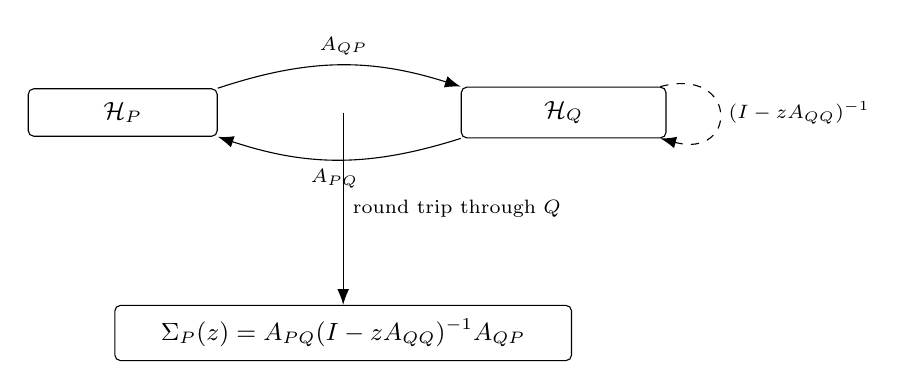
\begin{tikzpicture}[node distance=3.0cm]
  \node[ccbox, minimum width=2.4cm] (p) at (-2.8,0.8) {$\cH_P$};
  \node[ccbox, minimum width=2.6cm] (q) at (2.8,0.8) {$\cH_{\CCComp}$};
  \node[ccbox, align=center, minimum width=5.8cm] (sigma) at (0,-2.0)
    {$\CCSigmaP{P}{z}=\CCBlockPQ{A}(I-z\CCBlockQQ{A})^{-1}\CCBlockQP{A}$};

  \draw[ccarrow, bend left=18] (p.north east)
    to node[above, font=\scriptsize, pos=0.52] {$\CCBlockQP{A}$} (q.north west);
  \draw[ccarrow, bend left=18] (q.south west)
    to node[below, font=\scriptsize, pos=0.52] {$\CCBlockPQ{A}$} (p.south east);
  \draw[ccdarrow] (q) to[loop right, looseness=4]
    node[right, font=\scriptsize] {$(I-z\CCBlockQQ{A})^{-1}$} (q);
  \draw[ccarrow] ($(p)!0.5!(q)$) -- node[right, font=\scriptsize]
    {round trip through $\CCComp$} (sigma);
\end{tikzpicture}%
}
\caption{Schur complement / split transform: round-trip through $\CCComp$-block produces the Schur correction $\CCSigmaP{P}{z}$.}
\label{fig:schur-complement}
\end{figure}

\begin{quote}\small
\textbf{Intuition.}
The Schur correction $\CCSigmaP{P}{z}$ encodes how the $\CCComp$-degrees of freedom modify the effective resolvent.
$P$-states leak into $\CCComp$ ($\CCBlockQP{A}$), propagate there ($(I - z \CCBlockQQ{A})^{-1}$), and return ($\CCBlockPQ{A}$).
This round-trip contribution corrects the observed resolvent beyond the naive projection.
\end{quote}

\paragraph{Exact resummation.}
The identity is exact; no truncation or perturbative expansion is required.
The Schur correction $\CCSigmaP{P}{z}$ resums all paths through $\cH_{\CCComp}$ into a single correction term.
This is the Coherence Calculus mechanism for ``integrating out'' degrees of freedom.
The exact coherence and recovery theorems below show that, on a faithful tower,
this eliminated contribution remains part of the same underlying operator rather
than an added constitutive source.

\subsection{Residual signature (transport characterization)}

\begin{definition}[Transport blocks and residual signature]
\label{def:residual-signature}\lean{ResidualSignature}
For an operator $A$ and projection $P$, define:
\begin{itemize}[itemsep=0.2em]
\item \textbf{Transport out:} $\CCTransOut{P} := \CCBlockQP{A}$ (the $P \to \CCComp$ block).
\item \textbf{Transport in:} $\CCTransIn{P} := \CCBlockPQ{A}$ (the $\CCComp \to P$ block).
\item \textbf{Internal block:} $\CCBlockQQ{A}$ (the $\CCComp \to \CCComp$ block).
\end{itemize}
The \emph{residual signature} of $A$ with respect to $P$ is the triple $(\CCTransIn{P}, \CCBlockQQ{A}, \CCTransOut{P})$.
\end{definition}

\paragraph{Residual determines correction.}
The Schur correction is completely determined by the residual signature:
\[
\CCSigmaP{P}{z} = \CCTransIn{P} (I - z \CCBlockQQ{A})^{-1} \CCTransOut{P}.
\]
The round-trip factorization: transport out, propagate internally, transport back in.

\begin{definition}[Residual return field on a cut]
\label{def:residual-return-field}\lean{ResidualReturnField}
Fix an operator \(A\), a projection \(P\), and a shadow propagator
\[
R_Q=(I-z\CCBlockQQ{A})^{-1}
\]
whenever this inverse exists. The \emph{residual return field} generated by a
visible state \(u\in P\cH\) is the shadow datum
\[
\chi_{P,A,z}(u):=R_Q\,\CCTransOut{P}u.
\]
Its \emph{returned residual forcing} on the visible sector is
\[
\mathcal F^{\mathrm{return}}_{P,A,z}(u)
:=
\CCTransIn{P}\chi_{P,A,z}(u).
\]
\end{definition}

\begin{proposition}[Returned residual is exactly the Schur correction]
\label{prop:return-residual-is-schur}\lean{returnedResidual_eq_schur}
In the setting of Definition~\ref{def:residual-return-field},
\[
\mathcal F^{\mathrm{return}}_{P,A,z}(u)=\CCSigmaP{P}{z}u
\qquad (u\in P\cH).
\]
Thus the Schur correction is not an extra constitutive term. It is exactly the
visible trace of a residual field propagated in the eliminated sector and then
returned to observation.
\end{proposition}

(Proof in Appendix~\ref{sec:appendix-elimination}.)

\begin{corollary}[Self-adjoint structure]
\label{cor:self-adjoint-sigma}\lean{selfadjoint_block_relation}\lean{schur_selfadjoint_leading}
If $A$ is self-adjoint and $z \in \bbR$ with $(I - z\CCBlockQQ{A})^{-1}$ self-adjoint (holds when $z$ is not in the spectrum of $\CCBlockQQ{A}$ scaled appropriately), then:
\begin{enumerate}[label=(\roman*)]
\item $\CCTransIn{P} = (\CCTransOut{P})^*$, i.e., $\CCBlockPQ{A} = (\CCBlockQP{A})^*$.
\item $\CCSigmaP{P}{z}$ is self-adjoint on $\cH_P$.
\end{enumerate}
\end{corollary}

\begin{proof}
(i) For self-adjoint $A$: $(PAQ)^* = Q^* A^* P^* = QAP$, so $\CCBlockPQ{A}^* = \CCBlockQP{A}$.
(ii) $\CCSigmaP{P}{z}^* = (\CCBlockPQ{A} R_Q \CCBlockQP{A})^* = \CCBlockQP{A}^* R_Q^* \CCBlockPQ{A}^* = \CCBlockPQ{A} R_Q \CCBlockQP{A} = \CCSigmaP{P}{z}$.
\end{proof}

\subsection{Geometric series expansion}

\paragraph{Geometric series expansion.}
\label{rem:geometric-expansion}
If $\|z \CCBlockQQ{A}\| < 1$, then $(I - z \CCBlockQQ{A})^{-1} = \sum_{k=0}^\infty z^k (\CCBlockQQ{A})^k$ converges, giving
\[
\CCSigmaP{P}{z} = \sum_{k=0}^\infty z^k \CCBlockPQ{A} (\CCBlockQQ{A})^k \CCBlockQP{A}.
\]
This expands the Schur correction as a sum over ``$\CCComp$-excursions'' of increasing length.
The exact identity (Theorem~\ref{thm:feshbach-schur}) holds without this convergence assumption.

\paragraph{Connection to defect energy.}
When $P = \CCPi{h}$ and $A = d$ is a nilpotent differential, the leading term $\CCBlockPQ{A} \CCBlockQP{A} = \CCPi{h} d \CCPibar{h} \cdot \CCPibar{h} d \CCPi{h}$ is the defect operator $\CCDefect{d}{h}$ from the Horizon Fundamental Theorem (Section~\ref{sec:hft}).
The Schur correction generalizes this to all orders in $z$.

\subsection{Schur transport jets}
\label{subsec:schur-transport-jet}

\begin{definition}[Schur transport jet]
\label{def:schur-transport-jet}\lean{schur_transport_jet}
Let $(\CCPi{h})_{h\in\bbN}$ be a faithful horizon tower, let
$A:\cH\to\cH$ be bounded, and fix a horizon $h$. Assume
\[
\|z\,\CCPibar{h}A\CCPibar{h}\|<1.
\]
The \emph{Schur transport jet} at horizon $h$ is the family of operators
\[
K_{h,0}(A):=\CCPi{h}A\CCPi{h},
\qquad
K_{h,n}(A):=\CCPi{h}A(\CCPibar{h}A\CCPibar{h})^{n-1}\CCPibar{h}A\CCPi{h}
\quad(n\ge1),
\]
so that the effective operator admits the exact expansion
\[
\CCAeff{A}{\CCPi{h}}(z)=K_{h,0}(A)+\sum_{n\ge1} z^n K_{h,n}(A).
\]
\end{definition}

\begin{theorem}[Constructive order profile of the Schur transport jet]
\label{thm:schur-transport-jet-order}\lean{schur_transport_jet_order}
Assume the setting of Definition~\ref{def:schur-transport-jet}, and suppose the
underlying operator $A$ has tower transport order at most $r$ in the sense of
Definition~\ref{def:tower-transport-order}. Then:
\begin{enumerate}[label=(\roman*), leftmargin=2em, itemsep=0.2em]
\item $K_{h,0}(A)$ has order at most $r$;
\item for every $n\ge1$, the coefficient $K_{h,n}(A)$ has order at most
      $(n+1)r$;
\item the exact effective operator $\CCAeff{A}{\CCPi{h}}(z)$ therefore carries a
      constructive finite-order jet at every horizon, with order bounds
      determined solely by the tower order of $A$.
\end{enumerate}
\end{theorem}

(Proof in Appendix~\ref{sec:appendix-elimination}.)

\subsection{Stability bounds}

\begin{proposition}[Schur correction bound]
\label{prop:sigma-bound}\lean{schur_factorization_bound}
Assume $(I - z\CCBlockQQ{A})^{-1}$ exists with $\|(I - z\CCBlockQQ{A})^{-1}\| \le M$.
Then
\[
\|\CCSigmaP{P}{z}\| \;\le\; \|\CCBlockPQ{A}\| \cdot M \cdot \|\CCBlockQP{A}\|.
\]
\end{proposition}

\begin{proof}
$\|\CCSigmaP{P}{z}\| = \|\CCBlockPQ{A} (I - z\CCBlockQQ{A})^{-1} \CCBlockQP{A}\| \le \|\CCBlockPQ{A}\| \cdot \|(I - z\CCBlockQQ{A})^{-1}\| \cdot \|\CCBlockQP{A}\|$.
\end{proof}

\begin{proposition}[Perturbation stability]
\label{prop:perturbation-stability}\lean{PerturbationData}\lean{schurPerturbationDiff}
Let $A, \tilde{A}$ be operators with $E := \tilde{A} - A$.
Assume:
\begin{itemize}[itemsep=0.2em]
\item $(I - z\CCBlockQQ{A})^{-1}$ exists with $\|(I - z\CCBlockQQ{A})^{-1}\| \le M$.
\item $\|z \CCBlockQQ{E}\| \cdot M < 1$.
\end{itemize}
Then $(I - z\CCBlockQQ{\tilde{A}})^{-1}$ exists and
\[
\|\CCSigmaP{P}{z}[\tilde{A}] - \CCSigmaP{P}{z}[A]\|
\;\le\;
C(M, \|A\|, |z|) \cdot \|E\|,
\]
where
\[
C(M, \|A\|, |z|) = M^2 \bigl( 2 + |z| M (\|\CCBlockQQ{A}\| + \|E\|) \bigr) + M.
\]
\end{proposition}

\begin{proof}
Use the resolvent identity $(I - z\CCBlockQQ{\tilde{A}})^{-1} - (I - z\CCBlockQQ{A})^{-1} = z(I - z\CCBlockQQ{\tilde{A}})^{-1} \CCBlockQQ{E} (I - z\CCBlockQQ{A})^{-1}$.
The Neumann series gives $\|(I - z\CCBlockQQ{\tilde{A}})^{-1}\| \le M/(1 - |z| M \|\CCBlockQQ{E}\|)$.
Expand the difference $\CCSigmaP{P}{z}[\tilde{A}] - \CCSigmaP{P}{z}[A]$ using the product rule and collect terms.
\end{proof}

\subsection{Nested splits (band-by-band elimination)}

\begin{lemma}[Associativity of Schur complement]
\label{lem:nested-schur}\lean{NestedProjections}\lean{nestedSchurAssociativity}
Let $P_1, P_2$ be orthogonal projections with $P_1 \le P_2$ (i.e., $P_1 P_2 = P_1$).
Define $\CCComp_1 = I - P_1$ and $\CCComp_2 = I - P_2$, so $\CCComp_2 \le \CCComp_1$.
Under appropriate invertibility conditions, eliminating $\CCComp_1$ in two stages (first eliminate $\CCComp_2 \setminus P_2$, then eliminate $(P_2 \setminus P_1)$) equals direct elimination of $\CCComp_1$:
\[
\CCSigmaP{P_1}{z}[A] = \CCSigmaP{P_1}{z}[\CCAeff{A}{P_2}(z)].
\]
\end{lemma}

\begin{proof}
This follows from the associativity of Schur complements in block matrix theory: if $M$ is a $3 \times 3$ block matrix, the Schur complement onto the first block can be computed by first eliminating the third block, then the second.
The invertibility conditions transfer through the chain.
\end{proof}

\paragraph{Horizon-to-horizon elimination.}
When $P_1 = \CCPi{h}$ and $P_2 = \CCPi{h'}$ with $h < h'$, Lemma~\ref{lem:nested-schur} says we can eliminate from $h'$ to $h$ in one step, or go via intermediate levels.
This justifies recursive/hierarchical elimination schemes.

\subsection{Exact Schur towers and faithful recovery}
\label{subsec:exact-schur-towers}

\begin{definition}[Exact Schur tower at fixed parameter]
\label{def:exact-schur-tower-general}\lean{exact_schur_tower_general}
Let $(\CCPi{h})_{h\in\bbN}$ be a faithful horizon tower on a Hilbert space
$\cH$, let $A:\cH\to\cH$ be bounded, and fix
$z\in\mathbb{C}$ such that, for every $h$, the shadow resolvent
\[
(I-z\CCPibar{h}A\CCPibar{h})^{-1}
\]
exists. The associated \emph{exact Schur tower} is the family of effective
operators
\[
A_{\mathrm{eff},h}(z)
:=
\CCPi{h}A\CCPi{h}
+
z\,\CCPi{h}A\CCPibar{h}(I-z\CCPibar{h}A\CCPibar{h})^{-1}\CCPibar{h}A\CCPi{h}
=
\CCAeff{A}{\CCPi{h}}(z).
\]
\end{definition}

\begin{definition}[Schur coherence across nested horizons]
\label{def:schur-coherent-family-general}\lean{schur_coherent_family_general}
Let $\{A_{\mathrm{eff},h}(z)\}_{h\in\bbN}$ be the exact Schur tower of
Definition~\ref{def:exact-schur-tower-general}. For $h\le k$, let
\[
P_{h\mid k}:=\CCPi{h}\big|_{\CCPi{k}\cH}
\]
denote the induced orthogonal projection from the $k$th observed sector onto
the $h$th one. The family is \emph{Schur-coherent} if
\[
A_{\mathrm{eff},h}(z)
=
\CCAeff{A_{\mathrm{eff},k}(z)}{P_{h\mid k}}(z)
\qquad (h\le k).
\]
Thus cross-horizon compatibility is expressed by exact nested elimination,
rather than by literal intertwining of operators between different observed
sectors.
\end{definition}

\begin{theorem}[Exact Schur coherence of a bounded-operator tower]
\label{thm:exact-schur-coherence-general}\lean{exact_schur_coherence_general}
Let $(\CCPi{h})_{h\in\bbN}$ be a faithful horizon tower on $\cH$, let
$A:\cH\to\cH$ be bounded, and fix
$z\in\mathbb{C}$ such that every shadow resolvent
\[
(I-z\CCPibar{h}A\CCPibar{h})^{-1}
\]
exists. Then the exact Schur tower of
Definition~\ref{def:exact-schur-tower-general} is Schur-coherent in the sense
of Definition~\ref{def:schur-coherent-family-general}. Equivalently, for every
$h\le k$,
\[
\CCAeff{A}{\CCPi{h}}(z)
=
\CCAeff{\CCAeff{A}{\CCPi{k}}(z)}{P_{h\mid k}}(z).
\]
\end{theorem}

(Proof in Appendix~\ref{sec:appendix-elimination}.)

\begin{theorem}[Strong recovery of the underlying operator from the exact Schur tower]
\label{thm:schur-tower-strong-recovery-general}\lean{schur_tower_strong_recovery_general}
Let $(\CCPi{h})_{h\in\bbN}$ be a faithful horizon tower on a Hilbert space
$\cH$, let $A:\cH\to\cH$ be bounded, and fix
$z\in\mathbb{C}$ such that every shadow resolvent exists and satisfies the
uniform bound
\[
\sup_{h\in\bbN}
\left\|
(I-z\CCPibar{h}A\CCPibar{h})^{-1}
\right\|
\le M
\]
for some $M\ge 0$. Then for every $x\in\cH$,
\[
A_{\mathrm{eff},h}(z)x \to Ax
\qquad\text{as }h\to\infty,
\]
where $A_{\mathrm{eff},h}(z)$ is the exact Schur tower of
Definition~\ref{def:exact-schur-tower-general}.
\end{theorem}

(Proof in Appendix~\ref{sec:appendix-elimination}.)

\begin{remark}[Faithful recovery of the residual return field]
\label{rem:faithful-recovery-residual-return}
\lean{exact_schur_coherence_general, schur_tower_strong_recovery_general, nonlinear_shadow_elimination}
Together, Theorems~\ref{thm:exact-schur-coherence-general}
and \ref{thm:schur-tower-strong-recovery-general} show that a faithful exact
Schur tower recovers the underlying operator itself from the effective laws
seen at finite horizons. The residual return field of
Definition~\ref{def:residual-return-field} is therefore not a free source
insertion. Combined with exact nonlinear shadow elimination
(Theorem~\ref{thm:nonlinear-shadow-elimination}), this means that the residual
return field is an eliminated hidden datum whose returned visible trace is
exactly controlled by the same observed effective law; it is not an independent
postulate layered on top of that law.
\end{remark}

\begin{theorem}[Vanishing-normalized selected Schur families recover the same continuum operator]
\label{thm:selected-schur-recovery-general}\lean{selected_schur_recovery_general}
Let $(\CCPi{h})_{h\in\bbN}$ be a faithful horizon tower on $\cH$, let
$A:\cH\to\cH$ be bounded, and fix
$z\in\mathbb{C}$ such that the hypotheses of
Theorem~\ref{thm:schur-tower-strong-recovery-general} hold. For each horizon
$h$, let
\[
C_h:\CCPi{h}\cH\to\CCPi{h}\cH
\]
be any selected correction. Define the selected effective family by
\[
\widetilde A_h(z):=A_{\mathrm{eff},h}(z)+C_h.
\]
If
\[
\|C_h\CCPi{h}x\|\to 0
\qquad\text{for every }x\in\cH,
\]
then
\[
\widetilde A_h(z)x\to Ax
\qquad\text{for every }x\in\cH.
\]
\end{theorem}

(Proof in Appendix~\ref{sec:appendix-elimination}.)

\subsection{Corollary for horizon case}

\begin{corollary}[Horizon specialization]
\label{cor:horizon-specialization}\lean{HorizonSpecialization}\lean{horizon_schur_via_spec}
Setting $P = \CCPi{h}$ and $\CCComp = \CCPibar{h}$, all results in this section apply with:
\begin{align*}
\CCBlockPP{A} &= \CCRestr{A}{h}, & \CCBlockPQ{A} &= \CCPi{h} A \CCPibar{h}, \\
\CCBlockQP{A} &= \CCLeak{A}{h}, & \CCBlockQQ{A} &= \CCPibar{h} A \CCPibar{h}.
\end{align*}
The Schur correction becomes $\CCSigma{h}{z}$ as in the original notation.
\end{corollary}

\paragraph{Scale variation of resolvent.}
The horizon flow $\CCFlow{\cdot}{h}$ (Section~\ref{sec:advanced-operators}) applied to the observed resolvent $\CCPi{h} (I-zA)^{-1} \CCPi{h}$ provides a canonical scale variation operator for studying how the effective resolvent changes across coherence levels.

\subsection{Determinant factorization (finite-dimensional case)}

\begin{theorem}[Determinant factorization]
\label{thm:det-factorization}\lean{CoherenceCalculus.det_factorization}
Let $A:\cH \to \cH$ be a linear operator on a finite-dimensional Hilbert space with orthogonal projection $P$ and $\CCComp = I - P$.
For $z \in \mathbb{C}$ such that $(I - z\CCBlockQQ{A})$ is invertible, the characteristic determinant factors as:
\[
\det(I - zA) = \det(I - z\CCBlockQQ{A}) \cdot \det\bigl(I - z\CCAeff{A}{P}(z)\bigr),
\]
where $\CCAeff{A}{P}(z) = \CCBlockPP{A} + z\CCSigmaP{P}{z}$ is the effective operator (Definition~\ref{def:effective-operator}).
\end{theorem}

(Proof in Appendix~\ref{sec:appendix-elimination}.)

\begin{corollary}[Determinant ratio identity]
\label{cor:det-ratio}\lean{CoherenceCalculus.det_ratio}
Under the hypotheses of Theorem~\ref{thm:det-factorization}:
\[
\frac{\det(I - zA)}{\det(I - z\CCBlockQQ{A})} = \det\bigl(I - z\CCAeff{A}{P}(z)\bigr).
\]
This expresses the ``observable determinant ratio'' purely in terms of the effective operator.
\end{corollary}

\paragraph{Spectral interpretation.}
The identity separates the characteristic polynomial of $A$ into contributions from the $\CCComp$-block and the $P$-effective operator.
The roots of the left-hand side (eigenvalues of $A$ scaled by $1/z$) decompose into those ``coming from'' the shadow block and those ``coming from'' the effective observed dynamics.

\subsection{Functoriality under unitary conjugation}

\begin{theorem}[Conjugacy invariance of split transform]
\label{thm:split-functoriality}\lean{CoherenceCalculus.split_functoriality}
Let $U:\cH \to \cH$ be unitary, and define $P' := UPU^*$ and $A' := UAU^*$.
Then:
\begin{enumerate}[label=(\roman*)]
\item $\CCSigmaP{P'}{z}[A'] = U \CCSigmaP{P}{z}[A] U^*$.
\item $\CCAeff{A'}{P'}(z) = U \CCAeff{A}{P}(z) U^*$.
\end{enumerate}
In other words, the split transform commutes with unitary conjugation.
\end{theorem}

(Proof in Appendix~\ref{sec:appendix-elimination}.)

\paragraph{Symmetry inheritance.}
Theorem~\ref{thm:split-functoriality} implies that if a symmetry group $G$ acts unitarily on $\cH$ and preserves both $A$ and $P$ (i.e., $UAU^* = A$ and $UPU^* = P$ for all $U \in G$), then $G$ also preserves the Schur correction $\CCSigmaP{P}{z}$ and effective operator $\CCAeff{A}{P}(z)$.
This is the mechanism by which symmetry constraints propagate through the split transform.

\subsection{Exact nonlinear shadow elimination}

The linear Schur identity eliminates the shadow sector at the level of
resolvents. For nonlinear equations the correct analog is different in form but
identical in purpose: solve the shadow equation exactly as a graph over the
observed variables, then substitute that graph back into the observed equation.
The result is an exact reduced law on the observed sector, not an ansatz.

\begin{definition}[Nonlinear $P/Q$ split]
\label{def:nonlinear-pq-split}\lean{nonlinear_pq_split}
Let $P$ be an orthogonal projection on $\cH$, set $Q:=I-P$, and let
$\mathcal D\subseteq \cH$ be the domain of a map
$F:\mathcal D\to \cH$. For $(p,q)\in \cH_P\times\cH_Q$ with
$p+q\in\mathcal D$, define
\[
F_P(p,q):=PF(p+q),
\qquad
F_Q(p,q):=QF(p+q).
\]
Thus the equation $F(u)=0$ with $u=p+q$ is equivalent to the coupled system
\[
F_P(p,q)=0,
\qquad
F_Q(p,q)=0.
\]
\end{definition}

\begin{definition}[Exact nonlinear effective law]
\label{def:nonlinear-effective-law}\lean{nonlinear_effective_law}
Let $U_P\subseteq \cH_P$ and $U_Q\subseteq \cH_Q$. Suppose
$\Psi:U_P\to U_Q$ is a map such that $p+\Psi(p)\in\mathcal D$ for every
$p\in U_P$. The associated \emph{effective nonlinear law} on $U_P$ is
\[
F_{\mathrm{eff}}(p):=F_P\bigl(p,\Psi(p)\bigr)
=
P F\bigl(p+\Psi(p)\bigr).
\]
\end{definition}

\begin{theorem}[Exact nonlinear shadow elimination]
\label{thm:nonlinear-shadow-elimination}\lean{nonlinear_shadow_elimination}
Let $F:\mathcal D\to\cH$ be a map and let $P$ be an orthogonal projection with
$Q=I-P$. Let $U_P\subseteq \cH_P$ and $U_Q\subseteq \cH_Q$, and suppose that a
map $\Psi:U_P\to U_Q$ satisfies:
\begin{enumerate}[label=(\roman*), leftmargin=2em, itemsep=0.2em]
\item for every $p\in U_P$, one has $p+\Psi(p)\in\mathcal D$ and
      $F_Q\bigl(p,\Psi(p)\bigr)=0$;
\item whenever $p\in U_P$, $q\in U_Q$, $p+q\in\mathcal D$, and
      $F_Q(p,q)=0$, then $q=\Psi(p)$.
\end{enumerate}
Then the map
\[
p \longmapsto p+\Psi(p)
\]
is a bijection between the reduced solution set
\[
\{\,p\in U_P : F_{\mathrm{eff}}(p)=0\,\}
\]
and the full solution set
\[
\{\,u=p+q\in\mathcal D : p\in U_P,\ q\in U_Q,\ F(u)=0\,\}.
\]
Equivalently, on $U_P\times U_Q$ the full nonlinear equation $F(u)=0$ is
exactly equivalent to the reduced observed equation
\[
F_{\mathrm{eff}}(p)=0
\]
together with the reconstruction rule $q=\Psi(p)$.
\end{theorem}

(Proof in Appendix~\ref{sec:appendix-elimination}.)

\begin{figure}[ht]
\centering
\resizebox{0.8\textwidth}{!}{%
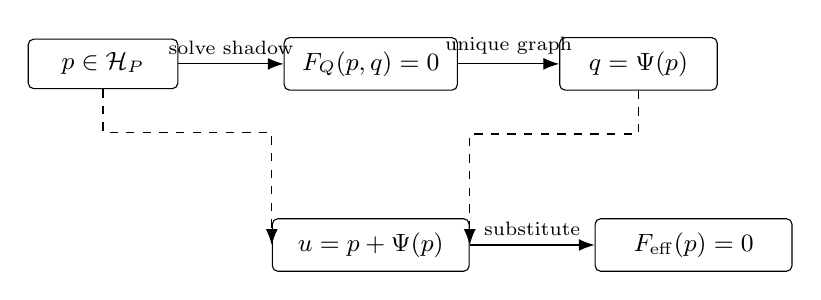
\begin{tikzpicture}[node distance=2.6cm]
  \node[ccbox, minimum width=1.9cm] (p) at (-4.3,1.2) {$p \in \cH_P$};
  \node[ccbox, minimum width=2.2cm] (shadow) at (-0.9,1.2) {$F_Q(p,q)=0$};
  \node[ccbox, minimum width=2.0cm] (psi) at (2.5,1.2) {$q=\Psi(p)$};
  \node[ccbox, minimum width=2.5cm] (u) at (-0.9,-1.1) {$u=p+\Psi(p)$};
  \node[ccbox, minimum width=2.5cm] (eff) at (3.2,-1.1) {$F_{\mathrm{eff}}(p)=0$};

  \draw[ccarrow] (p) -- node[above, cclabel] {solve shadow} (shadow);
  \draw[ccarrow] (shadow) -- node[above, cclabel] {unique graph} (psi);
  \draw[ccdarrow] (p.south) -- ++(0,-0.55) -| (u.west);
  \draw[ccdarrow] (psi.south) -- ++(0,-0.55) -| (u.east);
  \draw[ccarrow] (u) -- node[above, cclabel] {substitute} (eff);
\end{tikzpicture}%
}
\caption{Exact nonlinear elimination: solve the shadow equation for
$q=\Psi(p)$, then substitute into the observed equation.}
\label{fig:nonlinear-elimination}
\end{figure}

\begin{proposition}[Constructive semilinear shadow solve]
\label{prop:semicolon-shadow-elimination}\lean{semilinear_shadow_elimination}
Let
\[
F(u)=Lu+N(u)-f
\]
on a Hilbert space $\cH$, where $L:\cH\to\cH$ is bounded linear,
$N:\mathcal D\to\cH$ is a nonlinear map, and $f\in\cH$. Fix an orthogonal
projection $P$, set $Q:=I-P$, and let $B_P\subseteq \cH_P$ and
$B_Q\subseteq \cH_Q$ be sets such that $p+q\in\mathcal D$ for every
$p\in B_P$ and $q\in B_Q$, and with $B_Q$ complete in the ambient norm.
Assume:
\begin{enumerate}[label=(\roman*), leftmargin=2em, itemsep=0.2em]
\item $QLQ:\cH_Q\to\cH_Q$ is invertible;
\item for every $p\in B_P$, the map
      \[
      T_p(q):=(QLQ)^{-1}\bigl(Qf-QLP\,p-QN(p+q)\bigr)
      \]
      maps $B_Q$ into itself;
\item there exists $\kappa\in[0,1)$ such that for every $p\in B_P$ and all
      $q_1,q_2\in B_Q$,
      \[
      \|T_p(q_1)-T_p(q_2)\|\le \kappa \|q_1-q_2\|.
      \]
\end{enumerate}
Then:
\begin{enumerate}[label=(\roman*), leftmargin=2em, itemsep=0.2em]
\item for each $p\in B_P$ there exists a unique $\Psi(p)\in B_Q$ satisfying
      \[
      QF\bigl(p+\Psi(p)\bigr)=0;
      \]
\item the map $\Psi:B_P\to B_Q$ is given constructively by the fixed-point
      iteration $\Psi(p)=\lim_{n\to\infty}T_p^{\,n}(q_0)$ for any $q_0\in B_Q$;
\item the full semilinear equation $F(u)=0$ on
      $\{p+q:\,p\in B_P,\ q\in B_Q\}$ is exactly equivalent to the reduced law
      \[
      F_{\mathrm{eff}}(p)
      =
      \CCBlockPP{L}p + \CCBlockPQ{L}\Psi(p) + P N\bigl(p+\Psi(p)\bigr) - Pf
      =0.
      \]
\end{enumerate}
\end{proposition}

(Proof in Appendix~\ref{sec:appendix-elimination}.)

\begin{corollary}[Linear resolvent problem recovered]
\label{cor:linear-shadow-specialization}\lean{linear_shadow_specialization}
Let $F(u)=(I-zA)u-g$ with $A:\cH\to\cH$ linear, $g\in\cH$, and $P$ an
orthogonal projection. Assume $(I-z\CCBlockQQ{A})$ is invertible on
$\cH_{\CCComp}$. Then the unique shadow solve is
\[
\Psi(p)
=
(I-z\CCBlockQQ{A})^{-1}\bigl(Qg+z\CCBlockQP{A}p\bigr),
\]
and the reduced observed equation becomes
\[
\bigl(I-z\CCBlockPP{A}-z^2\CCSigmaP{P}{z}\bigr)p
=
Pg+z\CCBlockPQ{A}(I-z\CCBlockQQ{A})^{-1}Qg.
\]
In particular, if $Qg=0$, then the reduced law is
\[
\bigl(I-z\CCAeff{A}{P}(z)\bigr)p=Pg,
\]
so the linear Feshbach--Schur identity of
Theorem~\ref{thm:feshbach-schur} is recovered exactly.
\end{corollary}

(Proof in Appendix~\ref{sec:appendix-elimination}.)

\subsection{Global elimination and singular regimes}

The preceding proposition gives a constructive local theorem in a contraction
regime. The next results remove that smallness hypothesis on a large global
class and isolate the exact obstruction to further continuation.

\begin{theorem}[Global shadow elimination by strong monotonicity]\lean{global_monotone_shadow}
\label{thm:global-monotone-shadow}
Let $U_P\subseteq \cH_P$ and assume the shadow equation is defined on
$U_P\times \cH_Q$. For each $p\in U_P$, write
\[
G_p(q):=F_Q(p,q).
\]
Assume:
\begin{enumerate}[label=(\roman*), leftmargin=2em, itemsep=0.2em]
\item each $G_p:\cH_Q\to\cH_Q$ is hemicontinuous;
\item there exists $m>0$ such that for every $p\in U_P$ and all
      $q_1,q_2\in\cH_Q$,
      \[
      \operatorname{Re}\langle G_p(q_1)-G_p(q_2),\,q_1-q_2\rangle
      \ge
      m\|q_1-q_2\|^2;
      \]
\item each $G_p$ is coercive:
      \[
      \frac{\operatorname{Re}\langle G_p(q),q\rangle}{\|q\|}
      \longrightarrow +\infty
      \qquad\text{as }\|q\|\to\infty;
      \]
\item there exists $L\ge 0$ such that for every $p_1,p_2\in U_P$ and
      $q\in\cH_Q$,
      \[
      \|G_{p_1}(q)-G_{p_2}(q)\|\le L\|p_1-p_2\|.
      \]
\end{enumerate}
Then:
\begin{enumerate}[label=(\roman*), leftmargin=2em, itemsep=0.2em]
\item for every $p\in U_P$ there exists a unique $\Psi(p)\in\cH_Q$ such that
      $F_Q\bigl(p,\Psi(p)\bigr)=0$;
\item the shadow graph $\Psi:U_P\to\cH_Q$ is globally Lipschitz with
      \[
      \|\Psi(p_1)-\Psi(p_2)\|\le \frac{L}{m}\|p_1-p_2\|;
      \]
\item the full equation $F(u)=0$ on
      $\{\,p+q:\,p\in U_P,\ q\in\cH_Q\,\}$ is exactly equivalent to the
      reduced observed law
      \[
      F_{\mathrm{eff}}(p)=P F\bigl(p+\Psi(p)\bigr)=0.
      \]
\end{enumerate}
No Fredholm assumption is required.
\end{theorem}

(Proof in Appendix~\ref{sec:appendix-elimination}.)

\begin{theorem}[Regular and singular shadow regimes]\lean{regular_singular_shadow}
\label{thm:regular-singular-shadow}
Let $\mathcal O\subseteq \cH_P\times\cH_Q$ be open and suppose
$F_Q:\mathcal O\to\cH_Q$ is $C^1$. Define the regular and singular shadow sets
by
\[
\mathcal R
:=
\{(p,q)\in\mathcal O:\,F_Q(p,q)=0,\ D_qF_Q(p,q)\text{ is invertible}\}
\]
and
\[
\Sigma
:=
\{(p,q)\in\mathcal O:\,F_Q(p,q)=0,\ D_qF_Q(p,q)\text{ is not invertible}\}.
\]
Then every $(p_0,q_0)\in\mathcal R$ admits neighborhoods
$U\subseteq \cH_P$, $V\subseteq \cH_Q$ and a unique $C^1$ map
$\Psi:U\to V$ such that
\[
\Psi(p_0)=q_0
\qquad\text{and}\qquad
F_Q\bigl(p,\Psi(p)\bigr)=0
\quad \text{for all }p\in U.
\]
Moreover,
\[
D\Psi(p)
=
-\bigl[D_qF_Q\bigl(p,\Psi(p)\bigr)\bigr]^{-1}
  D_pF_Q\bigl(p,\Psi(p)\bigr).
\]
Thus $\Sigma$ is exactly the obstruction to local smooth shadow elimination.
\end{theorem}

\begin{proof}
This is the Banach-space implicit function theorem applied to the map
$F_Q$ at a zero $(p_0,q_0)$ with invertible vertical derivative
$D_qF_Q(p_0,q_0)$. The derivative formula follows by differentiating the
identity $F_Q(p,\Psi(p))=0$ and solving for $D\Psi(p)$.
\end{proof}

\begin{proposition}[Gauge-sliced shadow elimination]\lean{gauge_sliced_shadow}
\label{prop:gauge-sliced-shadow}
Assume a group $\Gamma$ acts on $\cH_Q$ by isometries. Let
$S\subseteq \cH_Q$ be a slice with the following properties:
\begin{enumerate}[label=(\roman*), leftmargin=2em, itemsep=0.2em]
\item the shadow equation is gauge-invariant in the sense that
      \[
      F_Q(p,\gamma\cdot q)=0
      \quad\Longleftrightarrow\quad
      F_Q(p,q)=0
      \qquad
      (\gamma\in\Gamma);
      \]
\item every $\Gamma$-orbit contained in the shadow zero set intersects $S$ in
      exactly one point.
\end{enumerate}
Then solving $F_Q(p,q)=0$ modulo gauge is equivalent to solving the restricted
equation
\[
F_Q(p,s)=0
\qquad\text{with } s\in S.
\]
If the restricted equation on $U_P\times S$ satisfies the hypotheses of
Theorem~\ref{thm:global-monotone-shadow} or
Theorem~\ref{thm:regular-singular-shadow}, then the full equation admits a
unique reduced observed law modulo gauge.
\end{proposition}

\begin{proof}
By gauge invariance, the shadow zero set is a union of $\Gamma$-orbits.
Assumption (ii) gives a bijection between those orbits and their unique slice
representatives in $S$. Therefore solving the shadow equation modulo gauge is
the same as solving it on the slice. The final statement is immediate from the
two cited theorems applied to the restricted equation.
\end{proof}

\paragraph{What is now solved, and what remains.}
The open problem of nonlinear elimination is resolved in the theoremic sense
needed by this manuscript. Exact elimination is now available:
\begin{enumerate}[label=(\roman*), leftmargin=2em, itemsep=0.2em]
\item locally by contraction in Proposition~\ref{prop:semicolon-shadow-elimination};
\item globally on a non-Fredholm class by strong monotonicity in
      Theorem~\ref{thm:global-monotone-shadow};
\item near regular singularity-free points by the implicit-function regime of
      Theorem~\ref{thm:regular-singular-shadow};
\item modulo gauge once a slice is fixed, by
      Proposition~\ref{prop:gauge-sliced-shadow}.
\end{enumerate}
What remains open is no longer elimination itself, but model-specific
verification of these hypotheses and branch selection on the singular set
$\Sigma$ when multiple continuations become admissible.

% ============================================================
\section{Observable-Relative Closure and Minimal Returned Data}
\label{sec:observable-relative-closure}
% ============================================================

\begin{quote}\small
\textbf{What this adds.}
The split and Schur calculus already determines the exact visible law and the
exact returned residual. What remains application-dependent is \emph{which}
visible outputs matter. This section makes that choice native: it records the
typed defect seen by a selected workload, the exact returned datum needed to
reconstruct that workload, and the finite-dimensional remainder seen after
Schur-jet truncation.

\smallskip\noindent
\textbf{Boundary.}
This is still operator-side calculus. It does not add new dynamics. It
composes the existing split and Schur operators with an explicit output map and
then studies the exact factorization profile of the resulting transfer.
\end{quote}

\subsection{Typed defects}

\begin{definition}[Typed coherence defect]
\label{def:typed-coherence-defect}\lean{CoherenceCalculus.typedCoherenceDefect}
Let \(X\) and \(Y\) be vector spaces, let \(P_X:X\to X\) and \(P_Y:Y\to Y\) be
projections, and let \(F:X\to Y\) be a map. The \emph{typed coherence defect}
of \(F\) at \(x\in X\) is
\[
\tau_{P_X,P_Y}(F;x):=P_YF(x)-F(P_Xx).
\]
\end{definition}

\begin{proposition}[Typed chain rule]
\label{prop:typed-chain-rule}\lean{CoherenceCalculus.typed_chain_rule}
Let \(F:Y\to Z\) and \(G:X\to Y\) be maps, and let \(P_X,P_Y,P_Z\) be
projections on \(X,Y,Z\), respectively. Then
\[
\tau_{P_X,P_Z}(F\circ G;x)
=
\tau_{P_Y,P_Z}(F;G(x))
+
\bigl(F(P_YG(x))-F(G(P_Xx))\bigr).
\]
If \(F\) is linear, the second term becomes \(F(\tau_{P_X,P_Y}(G;x))\).
\end{proposition}

\begin{proof}
\begin{align*}
\tau_{P_X,P_Z}(F\circ G;x)
&=
P_ZF(G(x))-F(G(P_Xx)) \\
&=
\bigl(P_ZF(G(x))-F(P_YG(x))\bigr)
+
\bigl(F(P_YG(x))-F(G(P_Xx))\bigr) \\
&=
\tau_{P_Y,P_Z}(F;G(x))
+
\bigl(F(P_YG(x))-F(G(P_Xx))\bigr).
\end{align*}
If \(F\) is linear, then
\[
F(P_YG(x))-F(G(P_Xx))
=
F\bigl(P_YG(x)-G(P_Xx)\bigr)
=
F(\tau_{P_X,P_Y}(G;x)).
\]
\end{proof}

\begin{definition}[Typed bilinear defect]
\label{def:typed-bilinear-defect}\lean{CoherenceCalculus.typedBilinearDefect}
Let \(X,Y,Z\) be vector spaces, let \(P_X,P_Y,P_Z\) be projections, and let
\(B:Y\times X\to Z\) be bilinear. The \emph{typed bilinear defect} is
\[
\tau_{P_Y,P_X,P_Z}(B;y,x):=
P_ZB(y,x)-B(P_Yy,P_Xx).
\]
\end{definition}

\begin{proposition}[Typed bilinear defect decomposition]
\label{prop:typed-bilinear-defect-decomposition}\lean{CoherenceCalculus.typed_bilinear_defect_decomposition}
Let \(Q_X:=I-P_X\) and \(Q_Y:=I-P_Y\). Assume the visible-visible closure
condition
\[
P_ZB(P_Yy,P_Xx)=B(P_Yy,P_Xx)
\qquad (x\in X,\ y\in Y).
\]
Then
\[
\tau_{P_Y,P_X,P_Z}(B;y,x)
=
P_ZB(P_Yy,Q_Xx)
+
P_ZB(Q_Yy,P_Xx)
+
P_ZB(Q_Yy,Q_Xx).
\]
\end{proposition}

(Proof in Appendix~\ref{sec:appendix-elimination}.)

\subsection{Observable packages and transfer operators}

\begin{definition}[Observable package]
\label{def:observable-package}\lean{CoherenceCalculus.ObservablePackage}
Let \(X\) be a vector space. An \emph{observable package} on \(X\) is a triple
\[
\Omega=(S,V,O)
\]
consisting of a source subspace \(S\subseteq X\), an output space \(V\), and a
linear observable map \(O:X\to V\).
\end{definition}

\begin{definition}[Paired observable package]
\label{def:paired-observable-package}\lean{CoherenceCalculus.PairedObservablePackage}
Let \(X\) and \(Y\) be vector spaces. A \emph{paired observable package} is a
triple
\[
\Omega=(S,T,B)
\]
consisting of a source subspace \(S\subseteq X\), a test subspace
\(T\subseteq Y\), and a bilinear pairing
\[
B:Y\times X\to \mathbb{R}
\qquad\text{or}\qquad
B:Y\times X\to \mathbb{C}.
\]
It induces the linear observable map
\[
O_T:X\to T^\ast,
\qquad
O_T(x):=B(\,\cdot\,,x)\big|_T.
\]
All linear observable-transfer statements below apply to \(O_T\).
\end{definition}

\begin{definition}[Direct observable transfer]
\label{def:direct-observable-transfer}\lean{CoherenceCalculus.directObservableTransfer}
Let \(\Omega=(S,V,O)\) be an observable package on \(X\), let \(P\) be a
projection on \(X\) with complement \(Q:=I-P\), and let \(A:X\to X\) be
linear. The \emph{direct observable transfer} is the map
\[
\mathfrak D_{\Omega}(P,A):=
OAQ\big|_{S}:S\to V.
\]
\end{definition}

\begin{proposition}[Exact direct observable decomposition]
\label{prop:direct-observable-decomposition}\lean{CoherenceCalculus.direct_observable_decomposition}
In the setting of Definition~\ref{def:direct-observable-transfer},
\[
O(Ax)=O(APx)+\mathfrak D_{\Omega}(P,A)x
\qquad (x\in S).
\]
In particular, if \(x\in S\cap PX\), then \(\mathfrak D_{\Omega}(P,A)x=0\).
\end{proposition}

\begin{proof}
Because \(I=P+Q\),
\[
Ax=A(P+Q)x=APx+AQx.
\]
Applying \(O\) gives
\[
O(Ax)=O(APx)+OAQx=O(APx)+\mathfrak D_{\Omega}(P,A)x.
\]
If \(x\in PX\), then \(Qx=0\), so the last term vanishes.
\end{proof}

\begin{definition}[Observable Schur return transfer]
\label{def:observable-schur-return-transfer}\lean{CoherenceCalculus.observableSchurReturnTransfer}
Let \(\Omega=(S,V,O)\) be an observable package on the Hilbert space
\(\cH\), let \(P\) be an orthogonal projection, and assume
\(\CCSigmaP{P}{z}\) is defined. On the visible workload
\[
S_P:=S\cap P\cH
\]
define the \emph{observable Schur return transfer} by
\[
\mathfrak R_{\Omega}(P,A;z)
:=
O\,\CCSigmaP{P}{z}\big|_{S_P}:S_P\to V.
\]
\end{definition}

\begin{definition}[Fixed-source observable Schur return transfer]
\label{def:fixed-source-observable-schur-return-transfer}\lean{CoherenceCalculus.fixedSourceObservableSchurReturnTransfer}
Let \(\Omega=(S,V,O)\) be an observable package on the Hilbert space
\(\cH\), let \(P\) be an orthogonal projection, and assume
\(\CCSigmaP{P}{z}\) is defined. The \emph{fixed-source observable Schur return
transfer} is
\[
\widetilde{\mathfrak R}_{\Omega}(P,A;z)
:=
O\,\CCSigmaP{P}{z}\,P\big|_{S}:S\to V.
\]
\end{definition}

\begin{proposition}[Returned residual seen by the workload]
\label{prop:observable-return-is-schur}\lean{CoherenceCalculus.observable_return_is_schur}
In the setting of Definition~\ref{def:observable-schur-return-transfer}, every
\(u\in S_P\) satisfies
\[
O\bigl(\mathcal F^{\mathrm{return}}_{P,A,z}(u)\bigr)
=
\mathfrak R_{\Omega}(P,A;z)u,
\]
and
\[
O\bigl(\CCAeff{A}{P}(z)u\bigr)
=
O(PAPu)+z\,\mathfrak R_{\Omega}(P,A;z)u.
\]
\end{proposition}

\begin{proof}
The first identity is Proposition~\ref{prop:return-residual-is-schur} composed
with \(O\):
\[
O\bigl(\mathcal F^{\mathrm{return}}_{P,A,z}(u)\bigr)
=
O\bigl(\CCSigmaP{P}{z}u\bigr)
=
\mathfrak R_{\Omega}(P,A;z)u.
\]
For the second identity, Definition~\ref{def:effective-operator} gives
\[
\CCAeff{A}{P}(z)u=PAPu+z\,\CCSigmaP{P}{z}u.
\]
Applying \(O\) and using the first identity yields the claim.
\end{proof}

\begin{proposition}[Fixed-source return restricts to the visible workload]
\label{prop:fixed-source-return-restricts}\lean{CoherenceCalculus.fixed_source_return_factorization, CoherenceCalculus.fixed_source_return_on_fixed_points}
In the setting of
Definitions~\ref{def:observable-schur-return-transfer}
and~\ref{def:fixed-source-observable-schur-return-transfer}, every
\(u\in S_P\) satisfies
\[
\widetilde{\mathfrak R}_{\Omega}(P,A;z)u
=
\mathfrak R_{\Omega}(P,A;z)u.
\]
If in addition \(P(S)\subseteq S\), then \(P\big|_S:S\to S_P\) and
\[
\widetilde{\mathfrak R}_{\Omega}(P,A;z)
=
\mathfrak R_{\Omega}(P,A;z)\circ P\big|_S.
\]
Consequently,
\[
\Img\bigl(\widetilde{\mathfrak R}_{\Omega}(P,A;z)\bigr)
=
\Img\bigl(\mathfrak R_{\Omega}(P,A;z)\bigr),
\]
hence the two return transfers have the same rank.
\end{proposition}

\begin{proof}
If \(u\in S_P\), then \(Pu=u\). Therefore
\[
\widetilde{\mathfrak R}_{\Omega}(P,A;z)u
=
O\,\CCSigmaP{P}{z}Pu
=
O\,\CCSigmaP{P}{z}u
=
\mathfrak R_{\Omega}(P,A;z)u.
\]
If \(P(S)\subseteq S\), then \(Px\in S_P\) for every \(x\in S\), so the
displayed factorization is exactly the identity just proved, applied to
\(u:=Px\).

Under the same hypothesis,
\(\Img(\widetilde{\mathfrak R}_{\Omega}(P,A;z))\subseteq
\Img(\mathfrak R_{\Omega}(P,A;z))\) by the factorization. For the reverse
inclusion, let \(y=\mathfrak R_{\Omega}(P,A;z)u\) with \(u\in S_P\). Since
\(u\in S\) and \(Pu=u\),
\[
y
=
\widetilde{\mathfrak R}_{\Omega}(P,A;z)u,
\]
so \(y\in \Img(\widetilde{\mathfrak R}_{\Omega}(P,A;z))\).
\end{proof}

\begin{remark}[Two return-transfer roles]
\label{rem:two-return-transfer-roles}\lean{CoherenceCalculus.observableSchurReturnTransfer, CoherenceCalculus.fixedSourceObservableSchurReturnTransfer, CoherenceCalculus.fixed_source_return_factorization, CoherenceCalculus.fixed_source_return_on_fixed_points}
The map \(\mathfrak R_{\Omega}(P,A;z)\) is the pointwise return seen on the
actual visible workload \(S_P=S\cap P\cH\). The map
\(\widetilde{\mathfrak R}_{\Omega}(P,A;z)\) keeps the source space fixed at
\(S\), so it is the correct object for comparing different cuts, taking ranks
and singular values across cuts, and formulating continuity on the
Grassmannian.
\end{remark}

\begin{proposition}[Continuity of the fixed-source return transfer]
\label{prop:fixed-source-return-continuity}\lean{CoherenceCalculus.FixedSourceReturnContinuityData, CoherenceCalculus.fixed_source_return_continuity}
Let \(\Omega=(S,V,O)\) be an observable package on a finite-dimensional
Hilbert space \(\cH\), let \(\mathcal U\) be a family of orthogonal
projections, and fix \(z\). Assume \(P\mapsto \CCSigmaP{P}{z}\) is continuous
on \(\mathcal U\) in operator norm. Then
\[
P\longmapsto \widetilde{\mathfrak R}_{\Omega}(P,A;z)
\]
is continuous on \(\mathcal U\) as a map into the operator space
\(\mathcal B(S,V)\).
\end{proposition}

\begin{proof}
Let \(P_n\to P\) in \(\mathcal U\). By hypothesis,
\(\CCSigmaP{P_n}{z}\to \CCSigmaP{P}{z}\) in operator norm. Therefore
\begin{align*}
\bigl\|
\widetilde{\mathfrak R}_{\Omega}(P_n,A;z)
-\widetilde{\mathfrak R}_{\Omega}(P,A;z)
\bigr\|_{\mathrm{op}}
&=
\bigl\|
O\bigl(\CCSigmaP{P_n}{z}P_n-\CCSigmaP{P}{z}P\bigr)\big|_S
\bigr\|_{\mathrm{op}} \\
&\le
\|O\|\,
\bigl\|
\CCSigmaP{P_n}{z}P_n-\CCSigmaP{P}{z}P
\bigr\|_{\mathrm{op}} \\
&\le
\|O\|\,
\Bigl(
\|\CCSigmaP{P_n}{z}-\CCSigmaP{P}{z}\|_{\mathrm{op}}\|P_n\|_{\mathrm{op}}
+ \|\CCSigmaP{P}{z}\|_{\mathrm{op}}\|P_n-P\|_{\mathrm{op}}
\Bigr) \\
&\le
\|O\|\,
\Bigl(
\|\CCSigmaP{P_n}{z}-\CCSigmaP{P}{z}\|_{\mathrm{op}}
+ \|\CCSigmaP{P}{z}\|_{\mathrm{op}}\|P_n-P\|_{\mathrm{op}}
\Bigr),
\end{align*}
because orthogonal projections have operator norm \(1\). The right-hand side
tends to \(0\), which proves continuity.
\end{proof}

\begin{definition}[Task-perfect coherence]
\label{def:task-perfect-coherence}\lean{CoherenceCalculus.taskPerfectCoherence}
Let \(\Omega=(S,V,O)\) be an observable package on \(\cH\). The pair
\((A,P)\) is \emph{task-perfect for \(\Omega\)} if
\[
\widetilde{\mathfrak R}_{\Omega}(P,A;z)=0
\]
for every \(z\) for which the Schur correction is defined.
\end{definition}

\begin{corollary}[Whole-state perfect coherence implies task-perfect coherence]
\label{cor:perfect-implies-task-perfect}\lean{CoherenceCalculus.perfect_implies_taskPerfect}
If \(\CCSigmaP{P}{z}=0\) for every \(z\) where defined, then \((A,P)\) is
task-perfect for every observable package \(\Omega=(S,V,O)\).
\end{corollary}

\begin{proof}
If \(\CCSigmaP{P}{z}=0\), then
\[
\widetilde{\mathfrak R}_{\Omega}(P,A;z)
=
O\,\CCSigmaP{P}{z}\,P\big|_{S}
=
0.
\]
\end{proof}

\subsection{Task-visible defect packages}

\begin{definition}[Source-visible loss]
\label{def:source-visible-loss}\lean{CoherenceCalculus.sourceVisibleLoss}
Let \(\Omega=(S,V,O)\) be an observable package on \(X\), and let \(P\) be a
projection on \(X\). The \emph{source-visible loss} of the cut \(P\) relative
to \(\Omega\) is
\[
\mathfrak S_{\Omega}(P):=O(I-P)\big|_S:S\to V.
\]
\end{definition}

\begin{definition}[Task-visible defect package]
\label{def:task-visible-defect-package}\lean{CoherenceCalculus.TaskVisibleDefectPackage, CoherenceCalculus.taskVisibleDefectPackage}
Let \(\Omega=(S,V,O)\) be an observable package on \(\cH\), let \(P\) be an
orthogonal projection, and assume \(\CCSigmaP{P}{z}\) is defined. The
\emph{task-visible defect package} is the triple
\[
\mathcal E_{\Omega}(P,A;z)
:=
\Bigl(
\mathfrak S_{\Omega}(P),\,
\mathfrak D_{\Omega}(P,A),\,
\widetilde{\mathfrak R}_{\Omega}(P,A;z)
\Bigr).
\]
\end{definition}

\begin{definition}[Task-visible faithfulness classes]
\label{def:task-visible-faithfulness}\lean{CoherenceCalculus.TaskVisibleFaithfulness}
Let \(\Omega=(S,V,O)\) be an observable package on \(\cH\).
\begin{enumerate}[label=(\roman*), leftmargin=2em, itemsep=0.2em]
\item The cut \(P\) is \emph{source-faithful for \(\Omega\)} if
      \[
      \mathfrak S_{\Omega}(P)=0.
      \]
\item The pair \((A,P)\) is \emph{one-step faithful for \(\Omega\)} if
      \[
      \mathfrak D_{\Omega}(P,A)=0.
      \]
\item The pair \((A,P)\) is \emph{task-exact for \(\Omega\)} if it is
      source-faithful, one-step faithful, and task-perfect.
\end{enumerate}
\end{definition}

\begin{remark}[What the defect package separates]
\label{rem:task-visible-defect-separation}\lean{CoherenceCalculus.sourceVisibleLoss, CoherenceCalculus.directObservableTransfer, CoherenceCalculus.fixedSourceObservableSchurReturnTransfer, CoherenceCalculus.taskVisibleDefectPackage}
These three channels measure different failures. Source-visible loss measures
what the cut removes before any dynamics act. Direct observable transfer
measures the one-step influence of the hidden source component. The fixed-source
Schur return transfer measures the hidden residual that re-enters after exact
elimination. The point of \(\mathcal E_{\Omega}(P,A;z)\) is that those failure
modes are no longer conflated.
\end{remark}

\subsection{Exact and approximate correction dimension}

\begin{theorem}[Exact correction factorization criterion]
\label{thm:exact-correction-factorization}\lean{CoherenceCalculus.ExactCorrectionFactorizationData, CoherenceCalculus.exact_correction_factorization}
Let \(T:S\to V\) and \(C:S\to R\) be linear maps. There exists a unique linear
map
\[
D_C:\Img(C)\to V
\]
with
\[
T=D_C\circ C
\]
if and only if
\[
\Ker(C)\subseteq \Ker(T).
\]
In finite dimensions, \(D_C\) extends to a linear decoder \(D:R\to V\) if one
wants a map on the whole correction space.
\end{theorem}

\begin{proof}
If \(T=D_C\circ C\) and \(Cx=0\), then \(Tx=D_C(Cx)=0\), so
\(\Ker(C)\subseteq\Ker(T)\).

Conversely, assume \(\Ker(C)\subseteq\Ker(T)\). Define \(D_C\) on \(\Img(C)\) by
\[
D_C(Cx):=Tx.
\]
This is well defined: if \(Cx=Cx'\), then \(C(x-x')=0\), so
\(x-x'\in\Ker(C)\subseteq\Ker(T)\), hence \(Tx=Tx'\).
If \(y\in\Img(C)\), write \(y=Cx\). Any linear map \(E:\Img(C)\to V\) with
\(T=E\circ C\) must satisfy
\[
E(y)=E(Cx)=Tx=D_C(Cx)=D_C(y),
\]
so \(E=D_C\). This proves uniqueness.
\end{proof}

\begin{remark}[Quotient-free exact correction]
\label{rem:quotient-free-exact-correction}\lean{CoherenceCalculus.ExactCorrectionFactorizationData, CoherenceCalculus.exact_correction_factorization}
The theorem is stated on \(\Img(C)\) rather than on the abstract quotient
\(S/\Ker(C)\). This is the exact same mathematical content, but it keeps the
factorization in an explicit image space and avoids introducing a quotient as a
primitive object.
\end{remark}

\begin{corollary}[Minimal exact correction dimension]
\label{cor:minimal-exact-correction-dimension}\lean{CoherenceCalculus.ObservableClosureRankData, CoherenceCalculus.observableClosureRank, CoherenceCalculus.minimal_exact_correction_dimension}
Let \(T:S\to V\) be linear with \(S\) and \(V\) finite-dimensional. The least
integer \(m\) for which there exist a space \(R\) with \(\dim R=m\) and maps
\[
C:S\to R,
\qquad
D:R\to V
\]
satisfying \(T=D\circ C\) is \(\rank(T)\).
\end{corollary}

\begin{proof}
Take \(R=\Img(T)\), let \(C:=T\), and let \(D:\Img(T)\hookrightarrow V\) be the
inclusion. Then \(T=D\circ C\) and \(\dim R=\rank(T)\).

Conversely, if \(T=D\circ C\), then
\[
\rank(T)\le \rank(C)\le \dim R.
\]
So every exact correction space has dimension at least \(\rank(T)\).
\end{proof}

\begin{definition}[Observable closure rank]
\label{def:observable-closure-rank}\lean{CoherenceCalculus.ObservableClosureRankData, CoherenceCalculus.observableClosureRank}
For a linear transfer \(T\), define its \emph{observable closure rank} by
\[
\rho(T):=\rank(T).
\]
If \(\Omega=(S,V,O)\) is an observable package in the Schur setting, define
\[
\rho_{\Omega}(P,A;z):=
\rank\bigl(\widetilde{\mathfrak R}_{\Omega}(P,A;z)\bigr).
\]
By Corollary~\ref{cor:minimal-exact-correction-dimension}, this is exactly the
minimal number of linear returned coordinates needed for exact closure of the
selected workload. If \(P(S)\subseteq S\), then
Proposition~\ref{prop:fixed-source-return-restricts} shows that this is also
the rank of the visible-workload return transfer
\(\mathfrak R_{\Omega}(P,A;z)\).
\end{definition}

\begin{corollary}[Zero rank is task-perfect coherence]
\label{cor:zero-closure-rank}\lean{CoherenceCalculus.zero_observable_closure_rank}
For every observable package \(\Omega=(S,V,O)\),
\[
\rho_{\Omega}(P,A;z)=0
\quad\Longleftrightarrow\quad
\widetilde{\mathfrak R}_{\Omega}(P,A;z)=0.
\]
\end{corollary}

\begin{proof}
A linear map has rank zero if and only if it is the zero map.
\end{proof}

\begin{definition}[Best \(m\)-dimensional correction error]
\label{def:best-m-correction-error}\lean{CoherenceCalculus.BestCorrectionErrorProfile, CoherenceCalculus.bestCorrectionError}
Let \(S\) and \(V\) be finite-dimensional normed spaces, let \(T:S\to V\) be
linear, and let \(m\in\bbN\). Define
\[
e_m(T):=
\inf_{\dim R\le m}
\inf_{C:S\to R,\ D:R\to V}
\|T-D\circ C\|_{\mathrm{op}}.
\]
\end{definition}

\begin{proposition}[Rank-constrained form and continuity of \(e_m\)]
\label{prop:best-m-correction-distance}\lean{CoherenceCalculus.CorrectionDistanceData, CoherenceCalculus.best_m_correction_distance}
Let \(S\) and \(V\) be finite-dimensional normed spaces. For every linear map
\(T:S\to V\),
\[
e_m(T)
=
\inf\{\|T-F\|_{\mathrm{op}}:\rank(F)\le m\}.
\]
Moreover, for all linear maps \(T,T':S\to V\),
\[
|e_m(T)-e_m(T')|
\le
\|T-T'\|_{\mathrm{op}}.
\]
\end{proposition}

\begin{proof}
If \(F=D\circ C\) with \(\dim R\le m\), then
\[
\rank(F)\le \rank(C)\le \dim R\le m.
\]
So every admissible factorization contributes a rank-at-most-\(m\) operator,
which proves
\[
e_m(T)\ge \inf\{\|T-F\|_{\mathrm{op}}:\rank(F)\le m\}.
\]

Conversely, if \(F:S\to V\) has \(\rank(F)\le m\), then \(F\) factors through
the \(m\)-dimensional space \(\Img(F)\): let
\[
C_F:S\to \Img(F),\qquad C_Fx:=Fx,
\]
and let \(D_F:\Img(F)\hookrightarrow V\) be the inclusion. Then
\[
F=D_F\circ C_F,
\]
so \(F\) is admissible in Definition~\ref{def:best-m-correction-error}. This
proves the rank-constrained formula.

For the Lipschitz bound, fix any rank-at-most-\(m\) operator \(F\). Then
\[
\|T-F\|_{\mathrm{op}}
\le
\|T-T'\|_{\mathrm{op}}+\|T'-F\|_{\mathrm{op}}.
\]
Taking the infimum over such \(F\) gives
\[
e_m(T)\le \|T-T'\|_{\mathrm{op}}+e_m(T').
\]
Interchanging \(T\) and \(T'\) yields the reverse inequality and hence the
claim.
\end{proof}

\subsection{Structured correction classes}

\begin{definition}[Structured correction class]
\label{def:structured-correction-class}\lean{CoherenceCalculus.StructuredCorrectionClass}
Let \(S\) and \(V\) be finite-dimensional normed spaces. For \(m\ge 0\), a
\emph{structured \(m\)-channel correction datum} from \(S\) to \(V\) is a
triple
\[
(R,C,D)
\]
where \(R\) is a vector space with \(\dim R\le m\), \(C:S\to R\) is linear,
and \(D:R\to V\) is linear. A \emph{structured correction class}
\(\mathcal C\) assigns to each \(m\ge 0\) a chosen subset
\[
\mathcal C_m(S,V)
\]
of such data.
\end{definition}

\begin{definition}[Structured closure width and structured closure rank]
\label{def:structured-closure-width}\lean{CoherenceCalculus.StructuredClosureProfile, CoherenceCalculus.structuredClosureWidth, CoherenceCalculus.structuredClosureRank}
Let \(\mathcal C\) be a structured correction class and let \(T:S\to V\) be
linear. Define the \emph{structured \(m\)-channel closure width} by
\[
e_m^{\mathcal C}(T)
:=
\inf_{(R,C,D)\in \mathcal C_m(S,V)}
\|T-D\circ C\|_{\mathrm{op}}.
\]
If there exists some \(m\) and some \((R,C,D)\in \mathcal C_m(S,V)\) with
\(T=D\circ C\), define the \emph{structured closure rank} \(\rho^{\mathcal C}(T)\)
to be the least such \(m\).
\end{definition}

\begin{proposition}[Universal lower envelope]
\label{prop:structured-width-lower-envelope}\lean{CoherenceCalculus.structured_width_lower_envelope}
Let \(\mathcal C\) be a structured correction class and let \(T:S\to V\) be
linear. Then
\[
e_m(T)\le e_m^{\mathcal C}(T)
\qquad (m\ge 0).
\]
If \(\rho^{\mathcal C}(T)\) is defined, then
\[
\rho(T)\le \rho^{\mathcal C}(T).
\]
\end{proposition}

\begin{proof}
Every datum \((R,C,D)\in \mathcal C_m(S,V)\) is in particular an admissible
\(m\)-channel correction datum in the sense of
Definition~\ref{def:best-m-correction-error}. Therefore the infimum over all
admissible data is bounded above by the infimum over the smaller structured
class.

If \(\rho^{\mathcal C}(T)=m\), then there exists
\((R,C,D)\in \mathcal C_m(S,V)\) with \(T=D\circ C\). Hence \(T\) admits an
exact \(m\)-channel factorization, so Corollary~\ref{cor:minimal-exact-correction-dimension}
gives \(\rho(T)\le m\).
\end{proof}

\begin{proposition}[Monotonicity for nested structured classes]
\label{prop:structured-width-monotonicity}\lean{CoherenceCalculus.structured_width_monotonicity}
Assume \(\mathcal C_m(S,V)\subseteq \mathcal C_{m+1}(S,V)\) for every \(m\).
Then
\[
e_{m+1}^{\mathcal C}(T)\le e_m^{\mathcal C}(T)
\qquad (m\ge 0).
\]
\end{proposition}

\begin{proof}
The infimum over the larger admissible set \(\mathcal C_{m+1}(S,V)\) cannot
exceed the infimum over the smaller set \(\mathcal C_m(S,V)\).
\end{proof}

\begin{remark}[Native examples]
\label{rem:structured-correction-native-examples}\lean{CoherenceCalculus.StructuredCorrectionClass, CoherenceCalculus.StructuredClosureProfile}
The class \(\mathcal C\) is where genuinely realizable restrictions enter:
equivariance, tower transport order, locality, block sparsity, or other
manuscript-native admissibility conditions. The unstructured width \(e_m\) is
the universal lower envelope; \(e_m^{\mathcal C}\) measures what remains once a
realizable design family is fixed.
\end{remark}

\subsection{Canonical optimal approximate correction}

\begin{definition}[Singular values]
\label{def:singular-values}\lean{CoherenceCalculus.SingularValueProfile, CoherenceCalculus.singularValue}
Let \(S\) and \(V\) be finite-dimensional inner-product spaces, and let
\(T:S\to V\) be linear. The \emph{singular values} of \(T\) are the nonnegative
numbers
\[
\sigma_1(T)\ge \sigma_2(T)\ge \cdots \ge \sigma_{\dim S}(T)\ge 0
\]
obtained by taking square roots of the eigenvalues of the positive
semidefinite operator \(T^\ast T\), repeated with multiplicity and listed in
nonincreasing order.
\end{definition}

\begin{theorem}[Optimal \(m\)-channel approximation]
\label{thm:optimal-m-channel-approximation}\lean{CoherenceCalculus.optimal_m_channel_approximation}
Let \(S\) and \(V\) be finite-dimensional inner-product spaces, let
\(T:S\to V\) be linear, and let
\[
\sigma_1(T)\ge \cdots \ge \sigma_{\dim S}(T)\ge 0
\]
be its singular values. Then there exist orthonormal vectors
\(u_1,\dots,u_{\dim S}\in S\) and an orthonormal family
\(v_1,\dots,v_r\in V\), where \(r=\rank(T)\), such that
\[
Tx=\sum_{i=1}^{r}\sigma_i(T)\,\langle x,u_i\rangle\,v_i
\qquad (x\in S).
\]
For \(m\ge 0\), define
\[
T^{[m]}x
:=
\sum_{i=1}^{\min(m,r)} \sigma_i(T)\,\langle x,u_i\rangle\,v_i.
\]
Then:
\begin{enumerate}[label=(\roman*), leftmargin=2em, itemsep=0.2em]
\item \(\rank(T^{[m]})\le m\);
\item \(e_m(T)=\|T-T^{[m]}\|_{\mathrm{op}}=\sigma_{m+1}(T)\), with the
      convention \(\sigma_{m+1}(T)=0\) when \(m\ge r\);
\item if \(U_m:=\Span\{u_1,\dots,u_{\min(m,r)}\}\), the orthogonal projector
      \(C_{T,m}:S\to U_m\) and the map \(D_{T,m}:U_m\to V\) defined by
      \[
      D_{T,m}(u_i):=\sigma_i(T)v_i
      \qquad
      (1\le i\le \min(m,r))
      \]
      satisfy
      \[
      T^{[m]}=D_{T,m}\circ C_{T,m}.
      \]
\end{enumerate}
\end{theorem}

(Proof in Appendix~\ref{sec:appendix-elimination}.)

\begin{corollary}[Optimal approximate returned correction for a workload]
\label{cor:optimal-returned-correction-for-workload}\lean{CoherenceCalculus.ObservableOptimalCorrectionData, CoherenceCalculus.optimal_returned_correction_for_workload}
Let \(\Omega=(S,V,O)\) be a finite-dimensional observable package on \(\cH\),
let \(P\) be an orthogonal projection, and assume
\(\widetilde{\mathfrak R}_{\Omega}(P,A;z)\) is defined. Then
\[
e_m\!\bigl(\widetilde{\mathfrak R}_{\Omega}(P,A;z)\bigr)
=
\sigma_{m+1}\!\bigl(\widetilde{\mathfrak R}_{\Omega}(P,A;z)\bigr).
\]
Accordingly, the visible workload admits an explicit optimal \(m\)-channel
returned correction obtained by truncating the singular expansion of the
observable Schur return transfer.
\end{corollary}

\begin{proof}
Apply Theorem~\ref{thm:optimal-m-channel-approximation} to the linear map
\[
T:=\widetilde{\mathfrak R}_{\Omega}(P,A;z):S\to V.
\]
\end{proof}

\begin{remark}[Canonicity and spectral gaps]
\label{rem:optimal-correction-gap}\lean{CoherenceCalculus.SingularValueProfile, CoherenceCalculus.optimal_m_channel_approximation}
If \(\sigma_m(T)>\sigma_{m+1}(T)\), then the leading singular subspace
\[
U_m=\Span\{u_i:\sigma_i(T)>\sigma_{m+1}(T)\}
\]
is uniquely determined by \(T^\ast T\), so the source projector \(C_{T,m}\) in
Theorem~\ref{thm:optimal-m-channel-approximation} is canonical. If
\(\sigma_m(T)=\sigma_{m+1}(T)\), then optimal \(m\)-channel corrections need
not be unique; the correct output is an optimal class rather than a singleton.
\end{remark}

\begin{remark}[Historical origin]
\label{rem:eckart-young-origin}\lean{CoherenceCalculus.optimal_m_channel_approximation}
The optimal low-rank approximation theorem is historically rooted in the work
of Eckart and Young, with the broader unitarily invariant norm perspective due
to Mirsky \cite{EckartYoung1936,Mirsky1960}. The proof used here is included
explicitly because later formal coverage must match the actual argument rather
than a citation boundary.
\end{remark}

\subsection{Design transforms and covariance}

\begin{definition}[Unitary design transform of a workload datum]
\label{def:observable-design-transform}\lean{CoherenceCalculus.ObservableDesignTransform}
Let \(U:\cH\to\cH\) be unitary. Define the transformed
operator, cut, and observable package by
\[
A^U:=UAU^{-1},
\qquad
P^U:=UPU^{-1},
\qquad
\Omega^U:=(US,V,OU^{-1}).
\]
\end{definition}

\begin{theorem}[Task-visible covariance under unitary design transforms]
\label{thm:observable-transfer-covariance}\lean{CoherenceCalculus.ObservableTransferCovarianceData, CoherenceCalculus.observable_transfer_covariance}
Let \(U:\cH\to\cH\) be unitary and write
\(\Omega=(S,V,O)\), \(\Omega^U=(US,V,OU^{-1})\),
\(A^U:=UAU^{-1}\), and \(P^U:=UPU^{-1}\). If
\(\CCSigmaP{P}{z}[A]\) is defined, then \(\CCSigmaP{P^U}{z}[A^U]\) is defined,
and
\[
\CCSigmaP{P^U}{z}[A^U]
=
U\,\CCSigmaP{P}{z}[A]\,U^{-1}.
\]
Moreover,
\[
\mathfrak S_{\Omega^U}(P^U)
=
\mathfrak S_{\Omega}(P)\circ U^{-1}\big|_{US},
\]
\[
\mathfrak D_{\Omega^U}(P^U,A^U)
=
\mathfrak D_{\Omega}(P,A)\circ U^{-1}\big|_{US},
\]
and
\[
\widetilde{\mathfrak R}_{\Omega^U}(P^U,A^U;z)
=
\widetilde{\mathfrak R}_{\Omega}(P,A;z)\circ U^{-1}\big|_{US}.
\]
\end{theorem}

\begin{proof}
Let \(Q:=I-P\). Then
\[
I-P^U
=
I-UPU^{-1}
=
U(I-P)U^{-1}
=
UQU^{-1}.
\]
Hence
\[
(I-P^U)A^U(I-P^U)
=
UQAQU^{-1}.
\]
Therefore
\[
I-z(I-P^U)A^U(I-P^U)
=
U(I-zQAQ)U^{-1},
\]
so invertibility of \(I-zQAQ\) implies invertibility of
\(I-z(I-P^U)A^U(I-P^U)\), with inverse
\[
\bigl(I-z(I-P^U)A^U(I-P^U)\bigr)^{-1}
=
U(I-zQAQ)^{-1}U^{-1}.
\]
Substituting this into the Schur formula gives
\begin{align*}
\CCSigmaP{P^U}{z}[A^U]
&=
P^U A^U (I-P^U)
\bigl(I-z(I-P^U)A^U(I-P^U)\bigr)^{-1}
(I-P^U)A^U P^U \\
&=
UPAQ(I-zQAQ)^{-1}QAPU^{-1} \\
&=
U\,\CCSigmaP{P}{z}[A]\,U^{-1}.
\end{align*}

For the source-visible loss,
\begin{align*}
\mathfrak S_{\Omega^U}(P^U)
&=
OU^{-1}(I-P^U)\big|_{US} \\
&=
OU^{-1}U(I-P)U^{-1}\big|_{US} \\
&=
O(I-P)U^{-1}\big|_{US}
=
\mathfrak S_{\Omega}(P)\circ U^{-1}\big|_{US}.
\end{align*}
The direct-transfer identity is the same computation with \(AQ\) in place of
\(I-P\):
\begin{align*}
\mathfrak D_{\Omega^U}(P^U,A^U)
&=
OU^{-1}A^U(I-P^U)\big|_{US} \\
&=
OAQ\,U^{-1}\big|_{US}
=
\mathfrak D_{\Omega}(P,A)\circ U^{-1}\big|_{US}.
\end{align*}
Finally,
\begin{align*}
\widetilde{\mathfrak R}_{\Omega^U}(P^U,A^U;z)
&=
OU^{-1}\,\CCSigmaP{P^U}{z}[A^U]\,P^U\big|_{US} \\
&=
OU^{-1}U\,\CCSigmaP{P}{z}[A]\,U^{-1}UPU^{-1}\big|_{US} \\
&=
O\,\CCSigmaP{P}{z}[A]\,P\,U^{-1}\big|_{US} \\
&=
\widetilde{\mathfrak R}_{\Omega}(P,A;z)\circ U^{-1}\big|_{US}.
\end{align*}
\end{proof}

\begin{proposition}[Source-isomorphism bounds for closure widths]
\label{prop:source-isomorphism-width-bounds}\lean{CoherenceCalculus.SourceIsomorphismWidthData, CoherenceCalculus.source_isomorphism_width_bounds}
Let \(W:S'\to S\) be an isomorphism between finite-dimensional normed spaces,
and let \(T:S\to V\) be linear. Then
\[
\|W^{-1}\|_{\mathrm{op}}^{-1}e_m(T)
\le
e_m(T\circ W)
\le
\|W\|_{\mathrm{op}}e_m(T).
\]
\end{proposition}

\begin{proof}
If \(F:S\to V\) has \(\rank(F)\le m\), then \(F\circ W:S'\to V\) also has rank
at most \(m\). Therefore
\[
e_m(T\circ W)
\le
\|T\circ W-F\circ W\|_{\mathrm{op}}
\le
\|T-F\|_{\mathrm{op}}\|W\|_{\mathrm{op}}.
\]
Taking the infimum over rank-at-most-\(m\) maps \(F\) gives the upper bound.

Now apply the same estimate to the pair \((T\circ W,W^{-1})\):
\[
e_m(T)
=
e_m\bigl((T\circ W)\circ W^{-1}\bigr)
\le
\|W^{-1}\|_{\mathrm{op}}\,e_m(T\circ W).
\]
Rearranging yields the lower bound.
\end{proof}

\begin{corollary}[Unitary invariance of workload closure data]
\label{cor:unitary-workload-invariance}\lean{CoherenceCalculus.UnitaryWorkloadInvarianceData, CoherenceCalculus.unitary_workload_invariance}
In the setting of Theorem~\ref{thm:observable-transfer-covariance}, assume
\(U\) is unitary. Then
\[
\rho_{\Omega^U}(P^U,A^U;z)=\rho_{\Omega}(P,A;z),
\]
\[
e_m\!\bigl(\widetilde{\mathfrak R}_{\Omega^U}(P^U,A^U;z)\bigr)
=
e_m\!\bigl(\widetilde{\mathfrak R}_{\Omega}(P,A;z)\bigr),
\]
and
\[
\sigma_i\!\bigl(\widetilde{\mathfrak R}_{\Omega^U}(P^U,A^U;z)\bigr)
=
\sigma_i\!\bigl(\widetilde{\mathfrak R}_{\Omega}(P,A;z)\bigr)
\qquad (1\le i\le \dim S).
\]
\end{corollary}

\begin{proof}
Let \(W:=U^{-1}\big|_{US}:US\to S\). Because \(U\) is unitary, \(W\) is
unitary as well, so \(\|W\|_{\mathrm{op}}=\|W^{-1}\|_{\mathrm{op}}=1\). The
covariance theorem gives
\[
\widetilde{\mathfrak R}_{\Omega^U}(P^U,A^U;z)
=
\widetilde{\mathfrak R}_{\Omega}(P,A;z)\circ W.
\]
Composition with the isomorphism \(W\) does not change rank, so the closure
rank is unchanged. Proposition~\ref{prop:source-isomorphism-width-bounds}
therefore gives equality of the widths \(e_m\). Finally,
Theorem~\ref{thm:optimal-m-channel-approximation} identifies
\(\sigma_i(T)\) with \(e_{i-1}(T)\), so equality of all widths implies
equality of all singular values.
\end{proof}

\subsection{Observable closure Gramians and invariants}

\begin{definition}[Observable closure Gramian]
\label{def:observable-closure-gramian}\lean{CoherenceCalculus.ObservableClosureGramianData, CoherenceCalculus.observableClosureGramian}
Let \(\Omega=(S,V,O)\) be a finite-dimensional observable package on \(\cH\),
and assume \(\widetilde{\mathfrak R}_{\Omega}(P,A;z)\) is defined. Set
\[
T_{\Omega,P,z}
:=
\widetilde{\mathfrak R}_{\Omega}(P,A;z):S\to V.
\]
The \emph{observable closure Gramian} is
\[
G_{\Omega}(P,A;z):=T_{\Omega,P,z}^\ast T_{\Omega,P,z}:S\to S.
\]
\end{definition}

\begin{definition}[Observable closure invariant family]
\label{def:observable-closure-invariants}\lean{CoherenceCalculus.ObservableClosureInvariantFamily, CoherenceCalculus.observableClosureInvariantFamilyOf}
In the setting of Definition~\ref{def:observable-closure-gramian}, define:
\begin{enumerate}[label=(\roman*), itemsep=0.2em]
\item the multiset
      \[
      \Lambda_{\Omega}(P,A;z):=
      \mathrm{spec}\bigl(G_{\Omega}(P,A;z)\bigr)
      \]
      of nonnegative eigenvalues of the closure Gramian;
\item the spectral moments
      \[
      M_k^{\Omega}(P,A;z):=
      \Tr\bigl(G_{\Omega}(P,A;z)^k\bigr)
      \qquad (k\ge 1);
      \]
\item the determinant polynomial
      \[
      \Delta_{\Omega}(P,A;z;t):=
      \det\bigl(I+tG_{\Omega}(P,A;z)\bigr).
      \]
\end{enumerate}
\end{definition}

\begin{theorem}[Finite observable closure package]
\label{thm:observable-closure-invariant-package}\lean{CoherenceCalculus.observable_closure_invariant_package}
Assume the setting of Definition~\ref{def:observable-closure-invariants}, and
let \(n:=\dim S\). Then:
\begin{enumerate}[label=(\roman*), itemsep=0.2em]
\item every element of \(\Lambda_{\Omega}(P,A;z)\) is nonnegative;
\item the following are equivalent:
      \[
      \Lambda_{\Omega}(P,A;z)=\{0,\dots,0\},
      \qquad
      G_{\Omega}(P,A;z)=0,
      \qquad
      \widetilde{\mathfrak R}_{\Omega}(P,A;z)=0;
      \]
\item if
      \[
      \Lambda_{\Omega}(P,A;z)=\{\lambda_1,\dots,\lambda_n\}
      \]
      with multiplicity in nonincreasing order, then
      \[
      \sigma_i\!\bigl(\widetilde{\mathfrak R}_{\Omega}(P,A;z)\bigr)
      =
      \sqrt{\lambda_i}
      \qquad (1\le i\le n),
      \]
      \[
      \rho_{\Omega}(P,A;z)=\#\{i:\lambda_i>0\},
      \qquad
      e_m\!\bigl(\widetilde{\mathfrak R}_{\Omega}(P,A;z)\bigr)
      =
      \sqrt{\lambda_{m+1}},
      \]
      with the convention \(\lambda_{m+1}=0\) for \(m\ge \rho_{\Omega}(P,A;z)\);
\item
      \[
      M_k^{\Omega}(P,A;z)=\sum_{i=1}^{n}\lambda_i^k,
      \qquad
      \Delta_{\Omega}(P,A;z;t)=\prod_{i=1}^{n}(1+t\lambda_i);
      \]
\item if \(U\) is unitary, then the transformed datum of
      Definition~\ref{def:observable-design-transform} has the same invariant
      family:
      \[
      \Lambda_{\Omega^U}(P^U,A^U;z)=\Lambda_{\Omega}(P,A;z),
      \]
      \[
      M_k^{\Omega^U}(P^U,A^U;z)=M_k^{\Omega}(P,A;z),
      \qquad
      \Delta_{\Omega^U}(P^U,A^U;z;t)=\Delta_{\Omega}(P,A;z;t).
      \]
\end{enumerate}
\end{theorem}

(Proof in Appendix~\ref{sec:appendix-elimination}.)

\begin{proposition}[Singular-value stability]
\label{prop:singular-value-stability}\lean{CoherenceCalculus.SingularValueStabilityData, CoherenceCalculus.singular_value_stability}
Let \(S\) and \(V\) be finite-dimensional inner-product spaces, and let
\(T,T':S\to V\) be linear. Then
\[
\bigl|\sigma_i(T)-\sigma_i(T')\bigr|
\le
\|T-T'\|_{\mathrm{op}}
\qquad (1\le i\le \dim S).
\]
\end{proposition}

\begin{proof}
By Theorem~\ref{thm:optimal-m-channel-approximation},
\[
\sigma_i(T)=e_{i-1}(T),
\qquad
\sigma_i(T')=e_{i-1}(T').
\]
Applying Proposition~\ref{prop:best-m-correction-distance} with \(m=i-1\)
gives the claim.
\end{proof}

\begin{corollary}[Continuity of the workload closure spectrum]
\label{cor:workload-closure-spectrum-continuity}\lean{CoherenceCalculus.WorkloadClosureSpectrumContinuityData, CoherenceCalculus.workload_closure_spectrum_continuity}
In the setting of Proposition~\ref{prop:fixed-source-return-continuity}, every
singular value
\[
P\longmapsto \sigma_i\!\bigl(\widetilde{\mathfrak R}_{\Omega}(P,A;z)\bigr)
\]
is continuous on the admissible cut family.
\end{corollary}

\begin{proof}
Combine Proposition~\ref{prop:fixed-source-return-continuity} with
Proposition~\ref{prop:singular-value-stability}.
\end{proof}

\subsection{Effective and null returned directions}

\begin{definition}[Observable null and effective projectors]
\label{def:observable-null-effective-projectors}\lean{CoherenceCalculus.ObservableEffectiveNullProjectors}
Let \(T:S\to V\) be linear between finite-dimensional inner-product spaces. The
\emph{observable null projector} and \emph{observable effective projector} are
\[
P_T^{\mathrm{null}}:=I-T^+T,
\qquad
P_T^{\mathrm{eff}}:=T^+T,
\]
where \(T^+\) is the Moore--Penrose pseudoinverse.
\end{definition}

\begin{proposition}[Effective/null decomposition of a returned residual]
\label{prop:observable-effective-null-decomposition}\lean{CoherenceCalculus.observable_effective_null_decomposition}
In the setting of
Definition~\ref{def:observable-null-effective-projectors},
\(P_T^{\mathrm{null}}\) is the orthogonal projector onto \(\Ker(T)\),
\(P_T^{\mathrm{eff}}\) is the orthogonal projector onto \((\Ker T)^\perp\), and
every \(r\in S\) decomposes as
\[
r=r_{\mathrm{eff}}+r_{\mathrm{null}},
\qquad
r_{\mathrm{eff}}:=P_T^{\mathrm{eff}}r,
\qquad
r_{\mathrm{null}}:=P_T^{\mathrm{null}}r,
\]
with
\[
T(r_{\mathrm{null}})=0,
\qquad
T(r)=T(r_{\mathrm{eff}}).
\]
\end{proposition}

\begin{proof}
Apply Lemma~\ref{lem:trace-ker} to the constraint map \(C:=T\) in
Appendix~\ref{sec:boundary-defect}. It shows that
\[
I-T^+T=P_T^{\mathrm{null}}
\]
is the orthogonal projector onto \(\Ker(T)\). Therefore
\[
P_T^{\mathrm{eff}}=I-P_T^{\mathrm{null}}
\]
is the orthogonal projector onto \((\Ker T)^\perp\). The displayed
decomposition is just
\[
r=P_T^{\mathrm{eff}}r+P_T^{\mathrm{null}}r.
\]
Since \(r_{\mathrm{null}}\in\Ker(T)\), we have \(T(r_{\mathrm{null}})=0\), and
hence
\[
T(r)=T(r_{\mathrm{eff}})+T(r_{\mathrm{null}})=T(r_{\mathrm{eff}}).
\]
\end{proof}

\begin{quote}\small
\textbf{Interpretation.}
For a selected workload, \(r_{\mathrm{null}}\) is the shadow component of a
returned residual that the workload never sees, while \(r_{\mathrm{eff}}\) is
the minimal Hilbert representative that carries exactly the observable effect.
\end{quote}

\subsection{Observable Schur jets}

\begin{definition}[Observable Schur-jet truncation]
\label{def:observable-schur-jet-truncation}\lean{CoherenceCalculus.ObservableSchurJetData, CoherenceCalculus.observableSchurJetTruncation}
Let \(\Omega=(S,V,O)\) be an observable package on \(\cH\), let \(P\) be an
orthogonal projection with \(Q:=I-P\), and assume \(\|zQAQ\|<1\). For
\(N\ge 1\), define the truncated observable return transfer
\[
\widetilde{\mathfrak R}_{\Omega}^{[N]}(P,A;z)
:=
O\left(
\sum_{n=0}^{N-1} z^n\,PAQ(QAQ)^nQAP
\right)P\Big|_{S}.
\]
\end{definition}

\begin{theorem}[Observable Schur-jet remainder]
\label{thm:observable-schur-jet-remainder}\lean{CoherenceCalculus.observable_schur_jet_remainder}
In the setting of Definition~\ref{def:observable-schur-jet-truncation},
\[
\widetilde{\mathfrak R}_{\Omega}(P,A;z)
-\widetilde{\mathfrak R}_{\Omega}^{[N]}(P,A;z)
=
O\Bigl(
z^N PAQ(QAQ)^N(I-zQAQ)^{-1}QAP
\Bigr)P\Big|_{S}.
\]
Consequently,
\[
\bigl\|
\widetilde{\mathfrak R}_{\Omega}(P,A;z)
-\widetilde{\mathfrak R}_{\Omega}^{[N]}(P,A;z)
\bigr\|_{\mathrm{op}}
\le
\|O\|\cdot \|PAQ\|\cdot \|zQAQ\|^N\cdot \|(I-zQAQ)^{-1}\|\cdot \|QAP\|.
\]
\end{theorem}

(Proof in Appendix~\ref{sec:appendix-elimination}.)

\begin{definition}[Observable closure order]
\label{def:observable-closure-order}\lean{CoherenceCalculus.ObservableClosureOrderData, CoherenceCalculus.observableClosureOrder}
In the setting of Definition~\ref{def:observable-schur-jet-truncation}, the
\emph{exact observable closure order} is the least \(N\ge 1\) such that
\[
\widetilde{\mathfrak R}_{\Omega}(P,A;z)
=
\widetilde{\mathfrak R}_{\Omega}^{[N]}(P,A;z).
\]
For a tolerance \(\varepsilon>0\), the \emph{\(\varepsilon\)-observable closure
order} is the least \(N\ge 1\) with
\[
\bigl\|
\widetilde{\mathfrak R}_{\Omega}(P,A;z)
-\widetilde{\mathfrak R}_{\Omega}^{[N]}(P,A;z)
\bigr\|_{\mathrm{op}}
\le \varepsilon.
\]
\end{definition}

\subsection{Stochastic and coded closure}

\begin{quote}\small
\textbf{Boundary.}
The deterministic transfer \(T\) remains primary. The stochastic layer does not
replace it; it studies how \(T\) can be realized by kernels and finite-bit
codes, with explicit mean, covariance, rate, entropy, and seed accounting.
\end{quote}

\begin{definition}[Support and probabilistic workload data]
\label{def:stochastic-workload-data}\lean{CoherenceCalculus.SupportWorkloadData, CoherenceCalculus.ProbabilisticWorkloadData}
Let \(S\) be a finite-dimensional Hilbert space and let \(T:S\to V\) be
linear.
\begin{enumerate}[label=(\roman*), leftmargin=2em, itemsep=0.2em]
\item A \emph{support workload datum} for \(T\) is a Borel set
      \[
      K\subseteq S.
      \]
\item A \emph{probabilistic workload datum} for \(T\) is a Borel probability
      measure \(\mu\in\mathcal P(S)\) with finite second moment:
      \[
      \int_S \|x\|^2\,d\mu(x)<\infty.
      \]
\end{enumerate}
\end{definition}

\begin{definition}[Stochastic closure kernel]
\label{def:stochastic-closure-kernel}\lean{CoherenceCalculus.StochasticClosureKernel}
Let \(K\subseteq S\) be a Borel workload set. A \emph{stochastic closure
kernel} from \(K\) to \(V\) is a Markov kernel
\[
\kappa:K\rightsquigarrow V
\]
such that
\[
\int_V \|v\|^2\,\kappa_x(dv)<\infty
\qquad (\forall x\in K).
\]
Its \emph{mean map} is
\[
M_{\kappa}(x):=\int_V v\,\kappa_x(dv),
\]
and its \emph{covariance operator field} is
\[
\Gamma_{\kappa}(x)
:=
\int_V (v-M_{\kappa}(x))\otimes(v-M_{\kappa}(x))\,\kappa_x(dv),
\]
where
\[
(u\otimes w)z:=u\,\langle z,w\rangle.
\]
\end{definition}

\begin{definition}[Exactness and unbiasedness]
\label{def:stochastic-exactness-unbiasedness}\lean{CoherenceCalculus.DeterministicZeroNoiseData}
Let \(T:K\to V\) be measurable and let \(\kappa\) be a stochastic closure
kernel on \(K\).
\begin{enumerate}[label=(\roman*), leftmargin=2em, itemsep=0.2em]
\item \(\kappa\) is \emph{exact} for \(T\) if
      \[
      \kappa_x=\delta_{T(x)}
      \qquad (\forall x\in K).
      \]
\item \(\kappa\) is \emph{unbiased} for \(T\) if
      \[
      M_{\kappa}(x)=T(x)
      \qquad (\forall x\in K).
      \]
\end{enumerate}
\end{definition}

\begin{theorem}[Pointwise bias--variance identity]
\label{thm:pointwise-bias-variance}\lean{CoherenceCalculus.StochasticBiasVarianceData, CoherenceCalculus.pointwise_bias_variance}
Let \(T:K\to V\) be measurable and let \(\kappa\) be a stochastic closure
kernel on \(K\). Then for every \(x\in K\),
\[
\int_V \|v-T(x)\|^2\,\kappa_x(dv)
=
\|M_{\kappa}(x)-T(x)\|^2
+
\Tr\Gamma_{\kappa}(x).
\]
\end{theorem}

\begin{proof}
Fix \(x\in K\), and write \(m:=M_{\kappa}(x)\), \(t:=T(x)\). Then
\[
v-t=(v-m)+(m-t),
\]
so
\[
\|v-t\|^2
=
\|v-m\|^2
+
2\,\mathrm{Re}\langle v-m,\ m-t\rangle
+
\|m-t\|^2.
\]
Integrating against \(\kappa_x\), the cross term vanishes because
\[
\int_V (v-m)\,\kappa_x(dv)=0.
\]
Therefore
\[
\int_V \|v-t\|^2\,\kappa_x(dv)
=
\int_V \|v-m\|^2\,\kappa_x(dv)
+
\|m-t\|^2.
\]
Since \(V\) is finite-dimensional,
\[
\int_V \|v-m\|^2\,\kappa_x(dv)=\Tr\Gamma_{\kappa}(x),
\]
which proves the identity.
\end{proof}

\begin{corollary}[Integrated bias--variance identity]
\label{cor:integrated-bias-variance}\lean{CoherenceCalculus.IntegratedBiasVarianceData, CoherenceCalculus.integrated_bias_variance}
Let \(\mu\) be a probabilistic workload datum for \(T\), and let \(\kappa\) be
a stochastic closure kernel on \(\operatorname{supp}\mu\). Then
\[
\int_S\int_V \|v-T(x)\|^2\,\kappa_x(dv)\,d\mu(x)
=
\|M_{\kappa}-T\|_{L^2(\mu;V)}^2
+
\int_S \Tr\Gamma_{\kappa}(x)\,d\mu(x).
\]
\end{corollary}

\begin{proof}
Integrate Theorem~\ref{thm:pointwise-bias-variance} against \(\mu\).
\end{proof}

\begin{proposition}[Zero covariance criterion]
\label{prop:zero-covariance-criterion}\lean{CoherenceCalculus.ZeroCovarianceCriterionData, CoherenceCalculus.zero_covariance_criterion}
Let \(\kappa\) be a stochastic closure kernel on \(K\). For a fixed \(x\in K\),
the following are equivalent:
\begin{enumerate}[label=(\roman*), leftmargin=2em, itemsep=0.2em]
\item \(\Gamma_{\kappa}(x)=0\);
\item \(\kappa_x=\delta_{M_{\kappa}(x)}\).
\end{enumerate}
\end{proposition}

\begin{proof}
If \(\kappa_x=\delta_{M_{\kappa}(x)}\), then the covariance is visibly zero.

Conversely, if \(\Gamma_{\kappa}(x)=0\), then
\[
0=\Tr\Gamma_{\kappa}(x)
=
\int_V \|v-M_{\kappa}(x)\|^2\,\kappa_x(dv),
\]
so \(v=M_{\kappa}(x)\) holds \(\kappa_x\)-almost surely. Therefore
\(\kappa_x=\delta_{M_{\kappa}(x)}\).
\end{proof}

\begin{corollary}[Deterministic closure as the zero-noise edge]
\label{cor:deterministic-zero-noise-edge}\lean{CoherenceCalculus.DeterministicZeroNoiseData, CoherenceCalculus.deterministic_zero_noise_edge}
Let \(T:K\to V\) be measurable and let \(\kappa\) be a stochastic closure
kernel on \(K\). Then \(\kappa\) is exact for \(T\) if and only if it is
unbiased for \(T\) and \(\Gamma_{\kappa}(x)=0\) for every \(x\in K\).
\end{corollary}

\begin{proof}
If \(\kappa_x=\delta_{T(x)}\), then \(M_{\kappa}(x)=T(x)\) and
\(\Gamma_{\kappa}(x)=0\).

Conversely, assume unbiasedness and zero covariance. By
Proposition~\ref{prop:zero-covariance-criterion},
\[
\kappa_x=\delta_{M_{\kappa}(x)}=\delta_{T(x)}
\qquad (\forall x\in K).
\]
\end{proof}

\begin{definition}[Seeded coded stochastic closure datum]
\label{def:seeded-coded-stochastic-closure-datum}\lean{CoherenceCalculus.SeededClosureCode}
Let \(K\subseteq S\) be a Borel workload set. A \emph{seeded coded stochastic
closure datum} from \(K\) to \(V\) is a quintuple
\[
\mathbf C=(\Xi,\pi,\mathcal A,\ell,(E,D))
\]
consisting of:
\begin{enumerate}[label=(\roman*), leftmargin=2em, itemsep=0.2em]
\item a standard Borel probability space \((\Xi,\pi)\), called the
      \emph{shared seed space};
\item a countable alphabet \(\mathcal A\);
\item a length function \(\ell:\mathcal A\to \bbN\) satisfying Kraft's
      inequality
      \[
      \sum_{a\in\mathcal A} 2^{-\ell(a)}\le 1;
      \]
\item a measurable encoder kernel
      \[
      E:K\times\Xi\rightsquigarrow \mathcal A;
      \]
\item a measurable decoder
      \[
      D:\mathcal A\times\Xi\to V.
      \]
\end{enumerate}
For \(x\in K\), \(\xi\in\Xi\), and \(a\in\mathcal A\), define the decoded
random output
\[
\widehat T_{\mathbf C}(x,\xi,a):=D(a,\xi).
\]
The induced stochastic closure kernel is
\[
\kappa^{\mathbf C}_x(B)
:=
\int_{\Xi}\sum_{a\in\mathcal A}
E_{x,\xi}(a)\,\mathbf 1_B\!\bigl(D(a,\xi)\bigr)\,d\pi(\xi).
\]
Its mean map and covariance field are
\[
M_{\mathbf C}:=M_{\kappa^{\mathbf C}},
\qquad
\Gamma_{\mathbf C}:=\Gamma_{\kappa^{\mathbf C}}.
\]
Unless explicitly stated otherwise, the rate functionals below charge the
emitted symbols but not the shared seed.
\end{definition}

\begin{definition}[Rate profiles]
\label{def:stochastic-rate-profiles}\lean{CoherenceCalculus.ClosureRateProfile, CoherenceCalculus.pointwiseCodeLength, CoherenceCalculus.worstCaseCodeLength, CoherenceCalculus.meanCodeLength}
Let \(\mathbf C\) be a seeded coded stochastic closure datum from a support
workload \(K\subseteq S\) to \(V\). Its pointwise expected code length is
\[
L_{\mathbf C}(x)
:=
\int_{\Xi}\sum_{a\in\mathcal A} E_{x,\xi}(a)\,\ell(a)\,d\pi(\xi).
\]
For a support workload \(K\subseteq S\), define
\[
L_K(\mathbf C):=\sup_{x\in K} L_{\mathbf C}(x).
\]
For a probabilistic workload datum \(\mu\) with
\(\operatorname{supp}\mu\subseteq K\), define
\[
L_{\mu}(\mathbf C):=\int_S L_{\mathbf C}(x)\,d\mu(x).
\]
\end{definition}

\begin{definition}[Rate-constrained stochastic closure widths]
\label{def:stochastic-closure-widths}\lean{CoherenceCalculus.ClosureWidthProfile, CoherenceCalculus.worstCaseClosureWidth, CoherenceCalculus.meanSquareClosureWidth, CoherenceCalculus.worstCaseUnbiasedClosureWidth, CoherenceCalculus.meanSquareUnbiasedClosureWidth}
Let \(T:K\to V\) be measurable, and let \(\mathcal C\) be an admissible class
of seeded coded stochastic closure data on \(K\).
\begin{enumerate}[label=(\roman*), leftmargin=2em, itemsep=0.2em]
\item The \emph{worst-case RMS stochastic closure width} at budget \(b\) is
      \[
      \eta^{\mathcal C}_{b,K}(T)
      :=
      \inf_{\mathbf C\in\mathcal C,\ L_K(\mathbf C)\le b}
      \sup_{x\in K}
      \Bigl(
      \mathbb E\|\widehat T_{\mathbf C}(x,\xi,a)-T(x)\|^2
      \Bigr)^{1/2}.
      \]
\item For a probabilistic workload datum \(\mu\) with
      \(\operatorname{supp}\mu\subseteq K\), the
      \emph{mean-square stochastic closure width} is
      \[
      \eta^{\mathcal C}_{b,\mu}(T)
      :=
      \inf_{\mathbf C\in\mathcal C,\ L_{\mu}(\mathbf C)\le b}
      \left(
      \int_S
      \mathbb E\|\widehat T_{\mathbf C}(x,\xi,a)-T(x)\|^2\,d\mu(x)
      \right)^{1/2}.
      \]
\item The corresponding \emph{unbiased widths}
      \(u^{\mathcal C}_{b,K}(T)\) and \(u^{\mathcal C}_{b,\mu}(T)\) are defined
      by the same formulas with the additional condition \(M_{\mathbf C}=T\).
\end{enumerate}
\end{definition}

\begin{proposition}[Monotonicity of stochastic closure widths]
\label{prop:stochastic-width-monotonicity}\lean{CoherenceCalculus.StochasticWidthMonotonicityData, CoherenceCalculus.stochastic_width_monotonicity}
If \(b'\ge b\), then
\[
\eta^{\mathcal C}_{b',K}(T)\le \eta^{\mathcal C}_{b,K}(T),
\qquad
\eta^{\mathcal C}_{b',\mu}(T)\le \eta^{\mathcal C}_{b,\mu}(T),
\]
and likewise for the unbiased widths. If \(\mathcal C\subseteq \mathcal C'\),
then
\[
\eta^{\mathcal C'}_{b,*}(T)\le \eta^{\mathcal C}_{b,*}(T),
\qquad
u^{\mathcal C'}_{b,*}(T)\le u^{\mathcal C}_{b,*}(T).
\]
\end{proposition}

\begin{proof}
Each inequality follows because the relevant infimum is taken over a larger
admissible set.
\end{proof}

\begin{definition}[Unseeded codebook datum]
\label{def:unseeded-codebook-datum}\lean{CoherenceCalculus.UnseededCodebook}
An \emph{unseeded codebook datum} on a support workload \(K\subseteq S\)
consists of a finite alphabet
\[
\mathcal A=\{1,\dots,N\},
\]
decoder atoms \(v_1,\dots,v_N\in V\), and a measurable map
\[
\lambda:K\to \Delta_N,
\]
where
\[
\Delta_N:=\left\{(\lambda_1,\dots,\lambda_N)\in [0,1]^N:
\sum_{i=1}^N\lambda_i=1\right\}.
\]
Its induced stochastic closure kernel is
\[
\kappa^{\lambda}_x
=
\sum_{i=1}^{N}\lambda_i(x)\,\delta_{v_i}.
\]
\end{definition}

\begin{theorem}[Barycentric exactness criterion]
\label{thm:barycentric-exactness-criterion}\lean{CoherenceCalculus.BarycentricExactnessData, CoherenceCalculus.barycentric_exactness_criterion}
Let \(T:K\to V\) be measurable. The following are equivalent:
\begin{enumerate}[label=(\roman*), leftmargin=2em, itemsep=0.2em]
\item there exists an unseeded finite-alphabet unbiased code for \(T\) with
      decoder atoms \(v_1,\dots,v_N\);
\item there exists a measurable \(\lambda:K\to\Delta_N\) such that
      \[
      T(x)=\sum_{i=1}^{N}\lambda_i(x)\,v_i
      \qquad (\forall x\in K).
      \]
\end{enumerate}
\end{theorem}

\begin{proof}
If such a code exists, let \(\lambda_i(x)\) be the probability that the encoder
emits symbol \(i\) at source point \(x\). Then the decoded mean is
\[
M(x)=\sum_{i=1}^{N}\lambda_i(x)\,v_i.
\]
Unbiasedness gives \(M(x)=T(x)\).

Conversely, given such a barycentric selector \(\lambda\), let the encoder
sample \(i\in\{1,\dots,N\}\) according to \(\lambda(x)\), and let the decoder
output \(v_i\). Then
\[
\mathbb E[\widehat T(x)]
=
\sum_{i=1}^{N}\lambda_i(x)\,v_i
=
T(x),
\]
so the resulting code is unbiased.
\end{proof}

\begin{definition}[Closure hull rank]
\label{def:closure-hull-rank}\lean{CoherenceCalculus.ClosureHullRankData, CoherenceCalculus.closureHullRank}
For a measurable target \(T:K\to V\), define its \emph{closure hull rank}
\[
\operatorname{hrk}_{K}(T)
\]
to be the least \(N\in\bbN\cup\{\infty\}\) such that there exist decoder atoms
\[
v_1,\dots,v_N\in V
\]
and a measurable barycentric selector \(\lambda:K\to \Delta_N\) satisfying
\[
T(x)=\sum_{i=1}^{N}\lambda_i(x)\,v_i
\qquad (\forall x\in K).
\]
\end{definition}

\begin{corollary}[Exact fixed-length stochastic rate]
\label{cor:exact-fixed-length-stochastic-rate}\lean{CoherenceCalculus.FixedLengthRateData, CoherenceCalculus.exact_fixed_length_stochastic_rate}
If \(\operatorname{hrk}_{K}(T)=N<\infty\), then \(T\) admits an exact unbiased
fixed-length code using \(\lceil \log_2 N\rceil\) bits per source instance.
Conversely, no exact unbiased fixed-length code with fewer than
\(\lceil \log_2 N\rceil\) bits exists.
\end{corollary}

\begin{proof}
If \(\operatorname{hrk}_{K}(T)=N\), Theorem~\ref{thm:barycentric-exactness-criterion}
gives an exact unbiased code with \(N\) symbols, which can be transmitted with
\(\lceil \log_2 N\rceil\) bits.

Conversely, a fixed-length \(b\)-bit code has at most \(2^b\) symbols. If such
a code were exact and unbiased, Theorem~\ref{thm:barycentric-exactness-criterion}
would imply \(\operatorname{hrk}_{K}(T)\le 2^b\). Hence
\[
b\ge \lceil \log_2 \operatorname{hrk}_{K}(T)\rceil.
\]
\end{proof}

\begin{example}[Exact one-bit unbiased scalar closure]
\label{ex:one-bit-unbiased-scalar-closure}\lean{CoherenceCalculus.OneBitUnbiasedScalarClosureData, CoherenceCalculus.one_bit_unbiased_scalar_closure}
Take
\[
S=V=\bbR,
\qquad
K=[-1,1],
\qquad
T(x)=x.
\]
Let the alphabet be \(\mathcal A=\{-1,+1\}\), with both symbols assigned length
\(1\), and define
\[
\mathbb P(a=+1\mid x)=\frac{1+x}{2},
\qquad
\mathbb P(a=-1\mid x)=\frac{1-x}{2}.
\]
Decode by
\[
D(+1)=1,
\qquad
D(-1)=-1.
\]
Then
\[
\mathbb E[\widehat T(x)]
=
\frac{1+x}{2}(1)+\frac{1-x}{2}(-1)
=
x,
\]
so the code is exact in expectation using one bit. Its variance is
\[
\mathbb E\bigl[(\widehat T(x)-x)^2\bigr]=1-x^2.
\]
\end{example}

\begin{definition}[Closure entropy profile]
\label{def:closure-entropy-profile}\lean{CoherenceCalculus.ClosureEntropyProfile, CoherenceCalculus.closureEntropy}
Let \(\mathbf C\) be a seeded coded stochastic closure datum. Define
\[
h_{\mathbf C}(x)
:=
\int_{\Xi} H(E_{x,\xi})\,d\pi(\xi),
\]
where the Shannon entropy in bits is
\[
H(p):=-\sum_{a\in\mathcal A} p(a)\log_2 p(a),
\]
with the convention \(0\log_2 0:=0\).
\end{definition}

\begin{theorem}[Entropy lower bound]
\label{thm:entropy-lower-bound}\lean{CoherenceCalculus.ClosureEntropyProfile, CoherenceCalculus.entropy_lower_bound}
Let \(\mathbf C\) be a seeded coded stochastic closure datum from a support
workload \(K\subseteq S\) to \(V\). Then
\[
h_{\mathbf C}(x)\le L_{\mathbf C}(x)
\qquad (\forall x\in K).
\]
If \(\mu\) is a probabilistic workload datum with
\(\operatorname{supp}\mu\subseteq K\), then
\[
\int_S h_{\mathbf C}(x)\,d\mu(x)\le L_{\mu}(\mathbf C).
\]
\end{theorem}

\begin{proof}
Fix \(x\in K\) and \(\xi\in\Xi\), and write \(p_a:=E_{x,\xi}(a)\). Set
\[
c_{\ell}:=\sum_{a\in\mathcal A}2^{-\ell(a)}\le 1,
\qquad
q_a:=\frac{2^{-\ell(a)}}{c_{\ell}}.
\]
Then
\begin{align*}
\sum_{a\in\mathcal A} p_a\,\ell(a)
&=
-\sum_{a\in\mathcal A} p_a \log_2 q_a-\log_2 c_{\ell} \\
&=
H(p)+D_{\mathrm{KL}}(p\|q)-\log_2 c_{\ell} \\
&\ge H(p),
\end{align*}
because \(D_{\mathrm{KL}}(p\|q)\ge 0\) and \(-\log_2 c_{\ell}\ge 0\). Integrate
first over \(\xi\). This gives \(h_{\mathbf C}(x)\le L_{\mathbf C}(x)\) for
every \(x\in K\). If \(\mu\) is a probabilistic workload datum supported in
\(K\), integrating that pointwise inequality against \(\mu\) yields the second
claim.
\end{proof}

\begin{remark}[Historical origin]
\label{rem:stochastic-coding-origin}\lean{CoherenceCalculus.ClosureEntropyProfile, CoherenceCalculus.entropy_lower_bound}
The entropy lower bound is the classical Shannon source-coding inequality built
on Kraft's inequality \cite{Shannon1948,Kraft1949}. The proof is included here
explicitly because later formal coverage must match the actual rate argument,
not a citation boundary.
\end{remark}

\begin{theorem}[Finite seed charging]
\label{thm:finite-seed-charging}\lean{CoherenceCalculus.FiniteSeedChargingData, CoherenceCalculus.finite_seed_charging}
Suppose a seeded coded stochastic closure datum \(\mathbf C\) has finite seed
set
\[
\Xi=\{\xi_1,\dots,\xi_M\}.
\]
Then there exists a seeded coded stochastic closure datum
\(\overline{\mathbf C}\) with one-point seed space, alphabet
\[
\Xi\times\mathcal A
\]
and lengths
\[
\bar\ell(\xi_i,a):=\ell(a)+\lceil \log_2 M\rceil
\]
whose decoded output law is identical to that of \(\mathbf C\).
\end{theorem}

\begin{proof}
Let the new seed space be the singleton \(\{\ast\}\). Define the new encoder by
\[
\overline E_{x,\ast}(\xi_i,a):=\pi(\{\xi_i\})\,E_{x,\xi_i}(a),
\]
and define the new decoder by
\[
\overline D((\xi_i,a),\ast):=D(a,\xi_i).
\]
Then, for every Borel set \(B\subseteq V\),
\[
\kappa^{\overline{\mathbf C}}_x(B)
=
\sum_{i=1}^M\sum_{a\in\mathcal A}
\pi(\{\xi_i\})\,E_{x,\xi_i}(a)\,
\mathbf 1_B\!\bigl(D(a,\xi_i)\bigr)
=
\kappa^{\mathbf C}_x(B),
\]
so the decoded output law is unchanged. Moreover,
\[
\sum_{i=1}^{M}\sum_{a\in\mathcal A}2^{-\bar\ell(\xi_i,a)}
=
\frac{M}{2^{\lceil \log_2 M\rceil}}
\sum_{a\in\mathcal A}2^{-\ell(a)}
\le 1,
\]
so the new lengths satisfy Kraft's inequality.
\end{proof}

\begin{theorem}[Linear output composition]
\label{thm:linear-output-composition}\lean{CoherenceCalculus.LinearOutputCompositionData, CoherenceCalculus.linear_output_composition}
Let \(L:V\to W\) be linear, and let \(\mathbf C\) be a seeded coded stochastic
closure datum for a target \(T:K\to V\). Define \(L\mathbf C\) by keeping the
same seed, alphabet, lengths, and encoder, and replacing the decoder by
\[
D_{L\mathbf C}:=L\circ D.
\]
Then
\[
M_{L\mathbf C}=L\circ M_{\mathbf C},
\]
\[
\Gamma_{L\mathbf C}(x)=L\,\Gamma_{\mathbf C}(x)\,L^\ast,
\]
and the rate profiles are unchanged:
\[
L_K(L\mathbf C)=L_K(\mathbf C),
\qquad
L_{\mu}(L\mathbf C)=L_{\mu}(\mathbf C).
\]
\end{theorem}

\begin{proof}
All claims follow from linearity of expectation, the identity
\[
(Lu)\otimes(Lu)=L(u\otimes u)L^\ast,
\]
and the fact that encoder, alphabet, and code lengths are unchanged.
\end{proof}

\begin{theorem}[Unitary source/output covariance of coded closure]
\label{thm:unitary-coded-closure-covariance}\lean{CoherenceCalculus.UnitaryCodedClosureCovarianceData, CoherenceCalculus.unitary_coded_closure_covariance}
Let \(U:S\to S\) and \(W:V\to V\) be unitary, let \(K\subseteq S\) be a support
workload, and define
\[
UK:=\{Ux:x\in K\},
\qquad
T^{U,W}:UK\to V,
\qquad
T^{U,W}(x'):=WT(U^{-1}x')).
\]
Given a seeded coded stochastic closure datum \(\mathbf C\) for \(T\), define
\(\mathbf C^{U,W}\) on \(UK\) by
\[
\bigl(E^{U,W}\bigr)_{x',\xi}(a):=E_{U^{-1}x',\xi}(a),
\qquad
D^{U,W}(a,\xi):=W D(a,\xi).
\]
Then
\[
M_{\mathbf C^{U,W}}(Ux)=W M_{\mathbf C}(x),
\]
\[
\Gamma_{\mathbf C^{U,W}}(Ux)=W\Gamma_{\mathbf C}(x)W^\ast,
\]
and the pointwise rate profiles are preserved:
\[
L_{\mathbf C^{U,W}}(Ux)=L_{\mathbf C}(x).
\]
If \(\mu\) is a probabilistic workload datum with \(\operatorname{supp}\mu
\subseteq K\), then for the pushforward measure \(U_{\ast}\mu\) on \(UK\),
\[
L_{U_{\ast}\mu}(\mathbf C^{U,W})=L_{\mu}(\mathbf C),
\]
\[
\|M_{\mathbf C^{U,W}}-T^{U,W}\|_{L^2(U_{\ast}\mu;V)}
=
\|M_{\mathbf C}-T\|_{L^2(\mu;V)},
\]
and
\[
\int_{UK}\Tr\Gamma_{\mathbf C^{U,W}}(x')\,d(U_{\ast}\mu)(x')
=
\int_{K}\Tr\Gamma_{\mathbf C}(x)\,d\mu(x).
\]
\end{theorem}

\begin{proof}
For \(x'\in UK\), write \(x:=U^{-1}x'\). By definition,
\[
\widehat T_{\mathbf C^{U,W}}(x',\xi,a)
=
W\widehat T_{\mathbf C}(x,\xi,a).
\]
Linearity of expectation gives the mean identity, and the covariance identity
follows from the same tensor identity used in
Theorem~\ref{thm:linear-output-composition}. The pointwise rate profile is
unchanged because the transformed encoder uses the same symbol law and the same
length function at the corresponding preimage point.

If \(\mu\) is supported in \(K\), the rate identity for \(U_{\ast}\mu\) follows
from the pointwise equality and the change of variables \(x'=Ux\). The same
change of variables, together with the unitarity of \(W\), yields the
\(L^2\)-identity for the mean defect and the integrated covariance identity.
\end{proof}

\begin{definition}[Closure covariance operator]
\label{def:closure-covariance-operator}\lean{CoherenceCalculus.ClosureCovarianceOperatorData, CoherenceCalculus.closureCovarianceOperator}
Let \(\mathbf C\) be a seeded coded stochastic closure datum from a support
workload \(K\subseteq S\) to \(V\), and let \(\mu\) be a probabilistic
workload datum with \(\operatorname{supp}\mu\subseteq K\). The \emph{closure
covariance operator} is
\[
\mathfrak C_{\mathbf C,\mu}(T)
:=
\int_S \Gamma_{\mathbf C}(x)\,d\mu(x).
\]
\end{definition}

\begin{proposition}[Positivity of closure covariance]
\label{prop:closure-covariance-positive}\lean{CoherenceCalculus.ClosureCovarianceOperatorData, CoherenceCalculus.closure_covariance_positive}
In the setting of Definition~\ref{def:closure-covariance-operator}, the
operator \(\mathfrak C_{\mathbf C,\mu}(T)\) is positive semidefinite.
\end{proposition}

\begin{proof}
For every \(w\in V\),
\[
\langle w,\mathfrak C_{\mathbf C,\mu}(T)w\rangle
=
\int_S \langle w,\Gamma_{\mathbf C}(x)w\rangle\,d\mu(x)\ge 0,
\]
because each covariance operator \(\Gamma_{\mathbf C}(x)\) is positive
semidefinite.
\end{proof}

\begin{corollary}[Integrated stochastic closure error]
\label{cor:integrated-stochastic-closure-error}\lean{CoherenceCalculus.ClosureCovarianceOperatorData, CoherenceCalculus.integrated_stochastic_closure_error}
In the setting of Definition~\ref{def:closure-covariance-operator},
\[
\int_S \mathbb E\|\widehat T_{\mathbf C}(x,\xi,a)-T(x)\|^2\,d\mu(x)
=
\|M_{\mathbf C}-T\|_{L^2(\mu;V)}^2
+
\Tr\mathfrak C_{\mathbf C,\mu}(T).
\]
If \(\mathbf C\) is unbiased for \(T\), then
\[
\int_S \mathbb E\|\widehat T_{\mathbf C}(x,\xi,a)-T(x)\|^2\,d\mu(x)
=
\Tr\mathfrak C_{\mathbf C,\mu}(T).
\]
\end{corollary}

\begin{proof}
Apply Corollary~\ref{cor:integrated-bias-variance} to the induced kernel
\(\kappa^{\mathbf C}\). The second identity is the unbiased case.
\end{proof}

\begin{definition}[Observable coded stochastic returned closure]
\label{def:observable-coded-stochastic-returned-closure}\lean{CoherenceCalculus.ObservableReturnedClosureCode}
Let \(\Omega=(S,V,O)\) be an observable package on \(\cH\), let \(P\) be an
orthogonal projection, and fix \(z\). Set
\[
T_{\Omega,P,z}:=
\widetilde{\mathfrak R}_{\Omega}(P,A;z):S\to V.
\]
An \emph{observable coded stochastic returned closure datum} is a seeded coded
stochastic closure datum for the target transfer \(T_{\Omega,P,z}\). Its
corrected observable estimator is
\[
\widehat{\mathcal O}_{\mathbf C,\Omega,P,z}(x,\xi,a)
:=
O(PAPx)+z\,\widehat T_{\mathbf C}(x,\xi,a).
\]
\end{definition}

\begin{theorem}[Unbiased returned correction]
\label{thm:unbiased-returned-correction}\lean{CoherenceCalculus.ObservableReturnedClosureCode, CoherenceCalculus.unbiased_returned_correction}
In the setting of
Definition~\ref{def:observable-coded-stochastic-returned-closure}, if
\(\mathbf C\) is unbiased for \(T_{\Omega,P,z}\), then
\[
\mathbb E\bigl[
\widehat{\mathcal O}_{\mathbf C,\Omega,P,z}(x,\xi,a)
\bigr]
=
O(PAPx)+z\,\widetilde{\mathfrak R}_{\Omega}(P,A;z)x.
\]
Hence the exact Schur-corrected observable law is recovered in expectation.
\end{theorem}

\begin{proof}
By linearity of expectation and unbiasedness,
\[
\mathbb E\bigl[
\widehat{\mathcal O}_{\mathbf C,\Omega,P,z}(x,\xi,a)
\bigr]
=
O(PAPx)+z\,\mathbb E[\widehat T_{\mathbf C}(x,\xi,a)]
=
O(PAPx)+z\,T_{\Omega,P,z}x.
\]
\end{proof}

\begin{corollary}[Observable mean-square error]
\label{cor:observable-mean-square-error}\lean{CoherenceCalculus.ObservableReturnedClosureCode, CoherenceCalculus.observable_mean_square_error}
In the setting of Theorem~\ref{thm:unbiased-returned-correction}, for every
\(x\in S\),
\[
\mathbb E\Bigl[
\bigl\|
\widehat{\mathcal O}_{\mathbf C,\Omega,P,z}(x,\xi,a)
-
\bigl(O(PAPx)+z\,T_{\Omega,P,z}x\bigr)
\bigr\|^2
\Bigr]
=
|z|^2\,\mathbb E\|\widehat T_{\mathbf C}(x,\xi,a)-T_{\Omega,P,z}x\|^2.
\]
\end{corollary}

\begin{proof}
The deterministic term \(O(PAPx)\) cancels, and multiplication by the scalar
\(z\) scales the squared norm by \(|z|^2\).
\end{proof}

\begin{remark}[Boundary of the coded layer]
\label{rem:coded-closure-boundary}\lean{CoherenceCalculus.SeededClosureCode, CoherenceCalculus.ClosureWidthProfile, CoherenceCalculus.ObservableReturnedClosureCode}
The present stochastic/coded layer is still calculus-internal: it packages
kernel realizations, prefix-code lengths, entropy lower bounds, seed
accounting, and mean/covariance control for a fixed task-visible transfer.
Specific one-bit sketches, quantizers, sparse codes, or hardware schemes are
not new primitives here; they enter only as explicit admissible classes
\(\mathcal C\) inside this layer.
\end{remark}

% ============================================================
\section{Variational-Discrete Realization and Crime Ledgers}
\label{sec:realization-calculus}
% ============================================================

\begin{quote}\small
\textbf{What this adds.}
The preceding sections determine exact visible laws, returned residuals,
workload-relative transfers, and coded closure data on the operator side. A
numerical host still has to realize those laws through weak forms, discrete
spaces, geometry maps, quadrature, stage splits, solver choices, and interface
transfers. This section makes that realization chain native.

\smallskip\noindent
\textbf{Boundary.}
This is a realization grammar, not a new foundation. It does not derive a
specific CFD, spectral-element, or CBS code from bedrock. It provides the
exact typed ledger in which any declared realization must record its departures
from exactness. Characteristic-based split schemes and high-order spectral
element hosts motivate this layer, but they enter only as external
realizations of the grammar developed here
\cite{NithiarasuCodinaZienkiewicz2006,Nek5000Theory2026,Nek5000CaseFiles2026,Nek5000Filters2026,NekNekTutorial2026}.
\end{quote}

\subsection{Variational laws and realization chains}

\begin{definition}[Variational law]
\label{def:variational-law}\lean{VariationalLaw}
A \emph{variational law} is a sextuple
\[
\mathcal V=(X,Y,a,\ell,\mathcal J,\mathcal I),
\]
where \(X\) and \(Y\) are finite-dimensional Hilbert spaces,
\[
a:X\times Y\to \bbR
\]
is a bilinear form,
\[
\ell:Y\to \bbR
\]
is a linear load functional,
\(\mathcal J\) is a declared family of linear observables on \(X\), and
\(\mathcal I\) is a declared family of linear invariants or constraints on
\(X\).
\end{definition}

\begin{definition}[Realization chain]
\label{def:realization-chain}\lean{RealizationChain}
Let \(\mathcal V=(X,Y,a,\ell,\mathcal J,\mathcal I)\) be a variational law. A
\emph{realization chain} at level \(h\) is a package
\[
\mathfrak R_h
=
(\mathcal V,X_h,Y_h,\Pi_h^X,\Pi_h^Y,\Phi_h,Q_h,\mathcal T_h,\mathcal S_h,\mathcal I_h)
\]
together with residual representatives
\[
R_h^{\mathrm{cont}},
\ R_h^{\mathrm{proj}},
\ R_h^{\mathrm{geom}},
\ R_h^{\mathrm{quad}},
\ R_h^{\mathrm{alias}},
\ R_h^{\mathrm{split}},
\ R_h^{\mathrm{lin}},
\ R_h^{\mathrm{alg}},
\ R_h^{\mathrm{bc}},
\ R_h^{\mathrm{iface}}
:X_h\times Y_h\to \bbR
\]
such that
\[
R_h^{\mathrm{cont}}(u_h,v_h)
:=
\ell(\Pi_h^Y v_h)-a(\Pi_h^X u_h,\Pi_h^Y v_h).
\]
The declared data have the following roles:
\begin{enumerate}[label=(\roman*), leftmargin=2em, itemsep=0.2em]
\item \(X_h,Y_h\) are the realized trial and test spaces.
\item \(\Pi_h^X,\Pi_h^Y\) map realized states and tests into the continuum
      law.
\item \(\Phi_h\) records geometry pullback/pushforward data.
\item \(Q_h\) records quadrature data.
\item \(\mathcal T_h\) records stage or time-splitting data.
\item \(\mathcal S_h\) records algebraic solver/preconditioner data.
\item \(\mathcal I_h\) records boundary and interface transfer data.
\end{enumerate}
The terminal residual
\[
R_h^{\mathrm{real}}:=R_h^{\mathrm{iface}}
\]
is the fully realized residual delivered by the declared host.
\end{definition}

\begin{definition}[Typed crime ledger]
\label{def:typed-crime-ledger}\lean{TypedCrimeLedger}\lean{typedCrimeLedger}
In the setting of Definition~\ref{def:realization-chain}, define the
\emph{typed realization crimes} by
\begin{align*}
\mathfrak C_h^{\mathrm{proj}} &:= R_h^{\mathrm{proj}}-R_h^{\mathrm{cont}},\\
\mathfrak C_h^{\mathrm{geom}} &:= R_h^{\mathrm{geom}}-R_h^{\mathrm{proj}},\\
\mathfrak C_h^{\mathrm{quad}} &:= R_h^{\mathrm{quad}}-R_h^{\mathrm{geom}},\\
\mathfrak C_h^{\mathrm{alias}} &:= R_h^{\mathrm{alias}}-R_h^{\mathrm{quad}},\\
\mathfrak C_h^{\mathrm{split}} &:= R_h^{\mathrm{split}}-R_h^{\mathrm{alias}},\\
\mathfrak C_h^{\mathrm{lin}} &:= R_h^{\mathrm{lin}}-R_h^{\mathrm{split}},\\
\mathfrak C_h^{\mathrm{alg}} &:= R_h^{\mathrm{alg}}-R_h^{\mathrm{lin}},\\
\mathfrak C_h^{\mathrm{bc}} &:= R_h^{\mathrm{bc}}-R_h^{\mathrm{alg}},\\
\mathfrak C_h^{\mathrm{iface}} &:= R_h^{\mathrm{iface}}-R_h^{\mathrm{bc}}.
\end{align*}
The tuple
\[
\mathfrak C_h
=
\bigl(
\mathfrak C_h^{\mathrm{proj}},
\mathfrak C_h^{\mathrm{geom}},
\mathfrak C_h^{\mathrm{quad}},
\mathfrak C_h^{\mathrm{alias}},
\mathfrak C_h^{\mathrm{split}},
\mathfrak C_h^{\mathrm{lin}},
\mathfrak C_h^{\mathrm{alg}},
\mathfrak C_h^{\mathrm{bc}},
\mathfrak C_h^{\mathrm{iface}}
\bigr)
\]
is the \emph{crime ledger} of the realization.
\end{definition}

\begin{theorem}[Exact residual ledger]
\label{thm:exact-residual-ledger}\lean{exact_residual_ledger}
For every realization chain,
\[
R_h^{\mathrm{real}}-R_h^{\mathrm{cont}}
=
\mathfrak C_h^{\mathrm{proj}}
+
\mathfrak C_h^{\mathrm{geom}}
+
\mathfrak C_h^{\mathrm{quad}}
+
\mathfrak C_h^{\mathrm{alias}}
+
\mathfrak C_h^{\mathrm{split}}
+
\mathfrak C_h^{\mathrm{lin}}
+
\mathfrak C_h^{\mathrm{alg}}
+
\mathfrak C_h^{\mathrm{bc}}
+
\mathfrak C_h^{\mathrm{iface}}
\]
pointwise on \(X_h\times Y_h\).
\end{theorem}

\begin{proof}
Substitute the definitions from Definition~\ref{def:typed-crime-ledger} and
sum. All intermediate residual representatives cancel telescopically:
\begin{align*}
\sum_{\alpha}\mathfrak C_h^{\alpha}
&=
\bigl(R_h^{\mathrm{proj}}-R_h^{\mathrm{cont}}\bigr)
+
\bigl(R_h^{\mathrm{geom}}-R_h^{\mathrm{proj}}\bigr)
+
\cdots
+
\bigl(R_h^{\mathrm{iface}}-R_h^{\mathrm{bc}}\bigr)\\
&=
R_h^{\mathrm{iface}}-R_h^{\mathrm{cont}}
=
R_h^{\mathrm{real}}-R_h^{\mathrm{cont}}.
\end{align*}
\end{proof}

\begin{corollary}[No hidden crime]
\label{cor:no-hidden-crime}\lean{no_hidden_crime}
If every typed crime in \(\mathfrak C_h\) vanishes, then
\[
R_h^{\mathrm{real}}=R_h^{\mathrm{cont}}.
\]
\end{corollary}

\begin{proof}
Apply Theorem~\ref{thm:exact-residual-ledger}.
\end{proof}

\begin{definition}[Realization exactness]
\label{def:realization-exactness}\lean{realizationExact}
A realization chain is \emph{realization-exact} if every entry of its crime
ledger vanishes identically.
\end{definition}

\subsection{Compatible mixed realization}

\begin{definition}[Fortin-compatible mixed realization]
\label{def:fortin-compatible-realization}\lean{FortinCompatibleRealization}
Let \(U\), \(U_h\), and \(M_h\) be finite-dimensional Hilbert spaces, and let
\[
b:U\times M_h\to \bbR,
\qquad
b_h:U_h\times M_h\to \bbR
\]
be continuous bilinear forms. A \emph{Fortin-compatible mixed realization}
consists of a linear lift
\[
F_h:U\to U_h
\]
and a constant \(C_F\ge 1\) such that
\[
b_h(F_hu,q_h)=b(u,q_h)
\qquad
(\forall u\in U,\ q_h\in M_h),
\]
and
\[
\|F_hu\|\le C_F\|u\|
\qquad
(\forall u\in U).
\]
\end{definition}

\begin{theorem}[Discrete inf-sup inherited from a Fortin lift]
\label{thm:discrete-infsup-from-fortin}\lean{discrete_infsup_from_fortin}
Assume the setting of Definition~\ref{def:fortin-compatible-realization}, and
suppose there is a constant \(\beta>0\) such that
\[
\sup_{u\in U\setminus\{0\}}
\frac{|b(u,q_h)|}{\|u\|}
\ge
\beta\|q_h\|
\qquad
(\forall q_h\in M_h).
\]
Then
\[
\sup_{u_h\in U_h\setminus\{0\}}
\frac{|b_h(u_h,q_h)|}{\|u_h\|}
\ge
\frac{\beta}{C_F}\|q_h\|
\qquad
(\forall q_h\in M_h).
\]
\end{theorem}

\begin{proof}
Fix \(q_h\in M_h\). By hypothesis, for every \(\varepsilon>0\) there exists
\(u\in U\setminus\{0\}\) such that
\[
|b(u,q_h)|
\ge
(\beta-\varepsilon)\|u\|\|q_h\|.
\]
Set \(u_h:=F_hu\). Then
\[
|b_h(u_h,q_h)|
=
|b(u,q_h)|
\ge
(\beta-\varepsilon)\|u\|\|q_h\|
\ge
\frac{\beta-\varepsilon}{C_F}\|u_h\|\|q_h\|.
\]
Taking the supremum over \(u_h\) and then letting \(\varepsilon\downarrow 0\)
gives the result.
\end{proof}

\begin{proposition}[Commuting constraint crime vanishes]
\label{prop:commuting-constraint-crime-vanishes}\lean{commuting_constraint_crime_vanishes}
Let \(B:U\to Z\), \(B_h:U_h\to Z_h\), and \(\Pi_h^Z:Z\to Z_h\) be linear maps.
If
\[
B_hF_h=\Pi_h^Z B,
\]
then the lifted constraint defect
\[
\mathfrak C_h^{\mathrm{compat}}(u):=B_hF_hu-\Pi_h^ZBu
\]
vanishes for every \(u\in U\).
\end{proposition}

\begin{proof}
This is exactly the stated commuting identity.
\end{proof}

\subsection{Geometry, quadrature, and aliasing}

\begin{definition}[Geometry-realized element form]
\label{def:geometry-realized-element-form}\lean{GeometryRealizedForm}
Let \(X_h\) and \(Y_h\) be realized spaces over an element family
\(\mathcal K_h\). For each \(K\in\mathcal K_h\), let
\[
\Phi_K:\widehat K\to K
\]
be a declared reference-to-physical map, and let
\[
\widehat g_{K,u_h,v_h}:\widehat K\to \bbR
\]
be the pulled-back integrand representing the local realized form. The
\emph{geometry-realized form} is
\[
a_h^{\mathrm{geom}}(u_h,v_h)
:=
\sum_{K\in\mathcal K_h}
\int_{\widehat K}\widehat g_{K,u_h,v_h}(\widehat x)\,d\widehat x.
\]
\end{definition}

\begin{definition}[Quadrature-realized form and crimes]
\label{def:quadrature-realized-form}\lean{QuadratureRealizedForm}
In the setting of Definition~\ref{def:geometry-realized-element-form}, let
\(Q_h=\{Q_K\}_{K\in\mathcal K_h}\) be elementwise quadrature rules and define
\[
a_h^Q(u_h,v_h)
:=
\sum_{K\in\mathcal K_h}Q_K[\widehat g_{K,u_h,v_h}].
\]
If \(a_h^{\mathrm{proj}}\) is a declared projected exact form on
\(X_h\times Y_h\), define the geometry and quadrature crimes by
\[
\mathfrak C_h^{\mathrm{geom}}(u_h,v_h)
:=
a_h^{\mathrm{geom}}(u_h,v_h)-a_h^{\mathrm{proj}}(u_h,v_h),
\]
\[
\mathfrak C_h^{\mathrm{quad}}(u_h,v_h)
:=
a_h^Q(u_h,v_h)-a_h^{\mathrm{geom}}(u_h,v_h).
\]
\end{definition}

\begin{theorem}[Geometry exactness kills geometry crime]
\label{thm:geometry-exactness-kills-geometry-crime}\lean{geometry_exactness_kills_geometry_crime}
If
\[
a_h^{\mathrm{geom}}(u_h,v_h)=a_h^{\mathrm{proj}}(u_h,v_h)
\qquad
(\forall u_h\in X_h,\ v_h\in Y_h),
\]
then \(\mathfrak C_h^{\mathrm{geom}}=0\).
\end{theorem}

\begin{proof}
This is the definition of \(\mathfrak C_h^{\mathrm{geom}}\).
\end{proof}

\begin{theorem}[Quadrature exactness kills quadrature crime]
\label{thm:quadrature-exactness-kills-quadrature-crime}\lean{quadrature_exactness_kills_quadrature_crime}
Assume that each element \(K\in\mathcal K_h\) carries a function class
\(\widehat{\mathfrak P}_K\) such that
\[
\widehat g_{K,u_h,v_h}\in \widehat{\mathfrak P}_K
\qquad
(\forall u_h\in X_h,\ v_h\in Y_h),
\]
and that
\[
Q_K[\varphi]=\int_{\widehat K}\varphi(\widehat x)\,d\widehat x
\qquad
(\forall \varphi\in \widehat{\mathfrak P}_K).
\]
Then \(\mathfrak C_h^{\mathrm{quad}}=0\).
\end{theorem}

\begin{proof}
For every \(u_h\in X_h\) and \(v_h\in Y_h\), the hypothesis gives
\[
Q_K[\widehat g_{K,u_h,v_h}]
=
\int_{\widehat K}\widehat g_{K,u_h,v_h}(\widehat x)\,d\widehat x
\qquad
(\forall K\in\mathcal K_h).
\]
Summing over elements yields \(a_h^Q(u_h,v_h)=a_h^{\mathrm{geom}}(u_h,v_h)\),
hence \(\mathfrak C_h^{\mathrm{quad}}(u_h,v_h)=0\).
\end{proof}

\begin{definition}[Paired aliasing package]
\label{def:paired-aliasing-package}\lean{PairedAliasingPackage}
Let \(S_h\subseteq X_h\) and \(T_h\subseteq Y_h\). The \emph{paired aliasing
package} associated with quadrature is
\[
\Omega_h^{\mathrm{alias}}=(S_h,T_h,B_h^{\mathrm{alias}}),
\]
where
\[
B_h^{\mathrm{alias}}(v_h,u_h):=\mathfrak C_h^{\mathrm{quad}}(u_h,v_h).
\]
\end{definition}

\begin{corollary}[Quadrature exactness kills workload-visible aliasing]
\label{cor:quadrature-exactness-kills-aliasing}\lean{quadrature_exactness_kills_aliasing}
If \(\mathfrak C_h^{\mathrm{quad}}=0\) on \(S_h\times T_h\), then the paired
aliasing package \(\Omega_h^{\mathrm{alias}}\) is zero on that workload, and
every one-sided observable transfer obtained from it by
Definition~\ref{def:paired-observable-package} also vanishes.
\end{corollary}

\begin{proof}
The first claim is exactly the definition of
\(B_h^{\mathrm{alias}}\). The induced one-sided observable transfers are
obtained by currying the same bilinear map, so they vanish as well.
\end{proof}

\begin{proposition}[Certified dealiasing on a selected workload]
\label{prop:certified-dealiasing-selected-workload}\lean{certified_dealiasing_selected_workload}
Let \(F_h:X_h\to X_h\) be linear. If
\[
\mathfrak C_h^{\mathrm{quad}}(F_hu_h,v_h)=0
\qquad
(\forall u_h\in S_h,\ v_h\in T_h),
\]
then the filtered workload \(F_hS_h\) is alias-free on the paired package
\(\Omega_h^{\mathrm{alias}}\).
\end{proposition}

\begin{proof}
This is the previous corollary applied to the filtered source family
\(F_hS_h\).
\end{proof}

\subsection{Stages, solvers, interfaces, and goals}

\begin{definition}[Stage bundle and split crime]
\label{def:stage-bundle-split-crime}\lean{StageBundle}\lean{stageBundleSplitCrime}
Let \(X_h\) be a realized state space. A \emph{stage bundle} at step
\(\Delta t\) is a composition
\[
\mathcal T_{\Delta t}
:=
\Psi^{(s)}_{\Delta t}\circ\cdots\circ\Psi^{(1)}_{\Delta t}
:X_h\to X_h.
\]
If \(\mathcal E_{\Delta t}:X_h\to X_h\) is a declared reference full-step
evolution, the \emph{split crime} is
\[
\mathfrak C_{\Delta t}^{\mathrm{split}}
:=
\mathcal T_{\Delta t}-\mathcal E_{\Delta t}.
\]
\end{definition}

\begin{proposition}[Stagewise invariants survive composition]
\label{prop:stagewise-invariants-survive-composition}\lean{stagewise_invariants_survive_composition}
Let \(I:X_h\to Z\) be any map. If
\[
I\circ \Psi^{(j)}_{\Delta t}=I
\qquad
(j=1,\dots,s),
\]
then
\[
I\circ\mathcal T_{\Delta t}=I.
\]
\end{proposition}

\begin{proof}
Apply the stage identities successively:
\[
I\circ\mathcal T_{\Delta t}
=
I\circ \Psi^{(s)}_{\Delta t}\circ\cdots\circ\Psi^{(1)}_{\Delta t}
=
I\circ \Psi^{(s-1)}_{\Delta t}\circ\cdots\circ\Psi^{(1)}_{\Delta t}
=
\cdots
=
I.
\]
\end{proof}

\begin{definition}[Solver package and algebraic crime]
\label{def:solver-package-algebraic-crime}\lean{SolverPackage}\lean{solverPackageAlgebraicCrime}
Let \(A_h:X_h\to X_h\) be a realized linear operator, let \(f_h\in X_h\), and
let \(\widetilde u_h\in X_h\) be a computed state. A \emph{solver package} is a
tuple
\[
\mathcal S_h=(A_h,M_h,\mathcal D_h,\mathcal P_h,\widetilde u_h),
\]
where \(M_h\) is a declared preconditioner, \(\mathcal D_h\) a declared
decomposition, and \(\mathcal P_h\) declared restriction/prolongation data. The
\emph{algebraic crime} is the residual
\[
r_h^{\mathrm{alg}}:=f_h-A_h\widetilde u_h.
\]
\end{definition}

\begin{theorem}[Exact solve iff algebraic crime vanishes]
\label{thm:exact-solve-iff-algebraic-crime-vanishes}\lean{exact_solve_iff_algebraic_crime_vanishes}
Assume \(A_h\) is invertible. Then
\[
r_h^{\mathrm{alg}}=0
\qquad\Longleftrightarrow\qquad
\widetilde u_h=A_h^{-1}f_h.
\]
\end{theorem}

\begin{proof}
If \(r_h^{\mathrm{alg}}=0\), then \(A_h\widetilde u_h=f_h\), so invertibility
forces \(\widetilde u_h=A_h^{-1}f_h\). The converse is immediate.
\end{proof}

\begin{proposition}[Spectral-equivalence solver certificate]
\label{prop:spectral-equivalence-solver-certificate}\lean{spectral_equivalence_solver_certificate}
Assume \(A_h\) and \(M_h\) are self-adjoint positive definite and that there
exist constants \(0<m\le M\) such that
\[
m\,\langle A_hx,x\rangle
\le
\langle M_hx,x\rangle
\le
M\,\langle A_hx,x\rangle
\qquad
(\forall x\in X_h).
\]
Then every eigenvalue \(\lambda\) of \(M_h^{-1}A_h\) lies in
\([
1/M,\,
1/m
]\),
so
\[
\kappa(M_h^{-1}A_h)\le M/m.
\]
\end{proposition}

\begin{proof}
Let \(A_hx=\lambda M_hx\) with \(x\ne 0\). Then
\[
\lambda
=
\frac{\langle A_hx,x\rangle}{\langle M_hx,x\rangle}.
\]
The spectral-equivalence bounds imply
\[
\frac{1}{M}
\le
\frac{\langle A_hx,x\rangle}{\langle M_hx,x\rangle}
\le
\frac{1}{m}.
\]
Thus \(\lambda\in[1/M,1/m]\), and the condition-number bound follows.
\end{proof}

\begin{definition}[Interface package and interface crime]
\label{def:interface-package-crime}\lean{InterfacePackage}\lean{interfaceCrime}
Let \(X_h\) and \(X_h^{\mathrm{ext}}\) be realized state spaces with trace maps
\[
\gamma_h:X_h\to \Lambda_h,
\qquad
\gamma_h^{\mathrm{ext}}:X_h^{\mathrm{ext}}\to \Lambda_h^{\mathrm{ext}}.
\]
An \emph{interface package} consists of a transfer map
\[
I_h:\Lambda_h^{\mathrm{ext}}\to \Lambda_h,
\]
a lift
\[
L_h:\Lambda_h\to X_h,
\]
and a declared host-transfer map
\[
T_h:X_h^{\mathrm{ext}}\to X_h.
\]
The \emph{interface crime} is
\[
\mathfrak C_h^{\mathrm{iface}}(u_h^{\mathrm{ext}})
:=
\gamma_hT_hu_h^{\mathrm{ext}}
-I_h\gamma_h^{\mathrm{ext}}u_h^{\mathrm{ext}}.
\]
\end{definition}

\begin{theorem}[Commuting interface diagrams kill interface crime]
\label{thm:commuting-interface-diagrams-kill-interface-crime}\lean{commuting_interface_diagrams_kill_interface_crime}
If
\[
\gamma_hT_h=I_h\gamma_h^{\mathrm{ext}},
\]
then \(\mathfrak C_h^{\mathrm{iface}}=0\). If moreover
\[
\gamma_hL_h=\operatorname{id}_{\Lambda_h},
\]
then the lifted interface correction \(L_h\mathfrak C_h^{\mathrm{iface}}\)
also vanishes.
\end{theorem}

\begin{proof}
The commuting identity is exactly the statement
\(\mathfrak C_h^{\mathrm{iface}}=0\). The second claim follows by applying
\(L_h\) to zero.
\end{proof}

\begin{definition}[Adjoint goal certificate]
\label{def:adjoint-goal-certificate}\lean{AdjointGoalCertificate}
Let \(A_h:X_h\to X_h\) be invertible and let \(\psi_h\in X_h\). The scalar goal
observable associated with \(\psi_h\) is
\[
J_{\psi_h}(v_h):=\langle \psi_h,v_h\rangle.
\]
The corresponding \emph{adjoint goal weight} is
\[
z_h:=(A_h^\ast)^{-1}\psi_h.
\]
\end{definition}

\begin{theorem}[Exact goal-error ledger identity]
\label{thm:exact-goal-error-ledger-identity}\lean{exact_goal_error_ledger_identity}
Let \(A_h:X_h\to X_h\) be invertible, let \(f_h\in X_h\), let
\(\widetilde u_h\in X_h\), and let
\[
u_h^\star:=A_h^{-1}f_h,
\qquad
e_h:=u_h^\star-\widetilde u_h,
\qquad
r_h:=f_h-A_h\widetilde u_h,
\]
and let \(z_h\) be the adjoint goal weight from
Definition~\ref{def:adjoint-goal-certificate}. If
\[
r_h=\sum_{\alpha} r_h^{\alpha},
\]
then
\[
J_{\psi_h}(e_h)
=
\langle z_h,r_h\rangle
=
\sum_{\alpha}\langle z_h,r_h^{\alpha}\rangle.
\]
\end{theorem}

\begin{proof}
Since \(A_hu_h^\star=f_h\),
\[
A_he_h
=
A_hu_h^\star-A_h\widetilde u_h
=
f_h-A_h\widetilde u_h
=
r_h.
\]
Therefore
\[
J_{\psi_h}(e_h)
=
\langle \psi_h,e_h\rangle
=
\langle A_h^\ast z_h,e_h\rangle
=
\langle z_h,A_he_h\rangle
=
\langle z_h,r_h\rangle.
\]
The final identity is linearity of the inner product.
\end{proof}

\begin{remark}[Realization certificates as tools]
\label{rem:realization-certificates-as-tools}\lean{exact_residual_ledger,discrete_infsup_from_fortin,geometry_exactness_kills_geometry_crime,quadrature_exactness_kills_quadrature_crime,stagewise_invariants_survive_composition,spectral_equivalence_solver_certificate,commuting_interface_diagrams_kill_interface_crime,exact_goal_error_ledger_identity}
The operator-side calculus already certifies visible/shadow splitting and
returned residuals. The present layer packages the complementary engineering
question: how a declared host realizes that law, and exactly where it does not.
The residual ledger, Fortin-compatible inheritance theorem, quadrature
exactness certificate, stagewise invariant theorem, spectral-equivalence
solver certificate, commuting-interface certificate, and dual-weighted
goal-error identity are the core theoremic outputs of this realization layer.
\end{remark}

% ============================================================
\section{Solver Layer: Exactness, Green Operators, and Homotopy}
\label{subsec:solver-layer}
% ============================================================

The preceding chapters require only projection algebra and additive closure.
Sometimes, however, the observable operator data sits inside a finite
Hilbert-complex package. In that case an additional solver layer becomes
available: exactness, Green operators, and canonical homotopies.

\begin{definition}[Finite Hilbert complex]
\label{def:hilbert-complex}\lean{finiteHilbertComplex}
A \emph{finite Hilbert complex} is a sequence of finite-dimensional inner
product spaces and linear maps
\[
0 \longrightarrow H^0 \xrightarrow{D_0} H^1 \xrightarrow{D_1} \cdots
\xrightarrow{D_{m-1}} H^m \longrightarrow 0
\]
such that
\[
D_{k+1} D_k = 0
\qquad
\text{for every } k.
\]
\end{definition}

\begin{definition}[Exactness]
\label{def:exactness}\lean{complexExactness}
The complex is \emph{exact at degree $k$} if
\[
\Ker(D_k) = \Img(D_{k-1}).
\]
Equivalently, the $k$th cohomology group vanishes:
\[
\CCCoh{k}(D) = 0.
\]
\end{definition}

\begin{definition}[Hodge Laplacian and Green operator]
\label{def:green-operator}\lean{hodgeLaplacian, greenOperator}
At degree $k$, define the Hodge Laplacian by
\[
\CCLap{k} := D_{k-1} D_{k-1}^* + D_k^* D_k.
\]
When $\CCLap{k}$ is invertible, its inverse
\[
\CCGreen{k} := \CCLap{k}^{-1}
\]
is the \emph{Green operator} at degree $k$.
\end{definition}

\begin{lemma}[Intertwining of the Laplacian with the differential]
\label{lem:laplacian-intertwining}\lean{laplacian_intertwines_differential}
For every degree $k$,
\[
D_k \CCLap{k} = \CCLap{k+1} D_k.
\]
Consequently, whenever the Green operators exist,
\[
D_k \CCGreen{k} = \CCGreen{k+1} D_k.
\]
\end{lemma}

(Proof in Appendix~\ref{sec:appendix-elimination}.)

\begin{theorem}[Homotopy identity with adjacent Green operators]
\label{thm:homotopy-identity}\lean{homotopyIdentity}
Assume the Green operators \(\CCGreen{k}\) and \(\CCGreen{k+1}\) both exist.
Define
\[
\CCHom{k} := D_{k-1}^* \CCGreen{k},
\qquad
\CCHom{k+1} := D_k^* \CCGreen{k+1}.
\]
Then
\[
D_{k-1} \CCHom{k} + \CCHom{k+1} D_k = I_{H^k}.
\]
\end{theorem}

(Proof in Appendix~\ref{sec:appendix-elimination}.)

\begin{remark}[Lean boundary for the solver layer]
\label{rem:solver-layer-lean-boundary}
\lean{homotopyIdentity}
On the active Lean surface, the homotopy identity is treated as an explicit
solver-interface property rather than as a bedrock theorem forced from
exactness alone. The theorem above is therefore one sufficient realization of
that interface when adjacent Green operators are available, not part of the
primitive calculus itself.
\end{remark}

\begin{definition}[Holographic saturation]
\label{def:holographic-saturation}\lean{holographicSaturation}
Let $R_k : H^k \to B^k$ be a boundary restriction map. The degree-$k$ layer is
\emph{holographically saturated} if
\[
\Ker(R_k) = \Img(D_{k-1}).
\]
Equivalently, the relative cohomology at degree $k$ vanishes:
\[
\CCCohRel{k}{D,R} = 0.
\]
\end{definition}

\paragraph{Scope of the solver layer.}
This layer is optional. It is not part of the bedrock axioms of the calculus.
Rather, it is the exact package that becomes available once the operator data
is known to form an exact finite Hilbert complex.

% ============================================================
\section{Targets and Certifications}
\label{sec:targets}
% ============================================================

\begin{quote}\small
\textbf{Goal:} Catalog the structural and objective targets in Coherence Calculus.\\
\textbf{Structural targets} are exact certification statements: properties that can be certified directly from the active interfaces, either on the whole visible state or on a selected workload.\\
\textbf{Objective targets} are optimization problems: find a projection that minimizes/maximizes a functional.
\end{quote}

% ------------------------------------------------------------
\subsection{Structural Targets (Iff Theorems)}
\label{subsec:structural-targets}
% ------------------------------------------------------------

Structural targets are exact certifications on the active interface surface.
Some are equivalences, while others are one-way sufficient criteria.
No approximation or optimization is required; only verification.

\paragraph{A) Perfect Coherence (Zero Residual)}

\begin{definition}[Perfect coherence]
\label{def:perfect-coherence}\lean{CoherenceCalculus.hasPerfectCoherence}
An operator $A$ has \emph{perfect coherence} with respect to projection $P$ if the Schur correction vanishes:
\[
\CCSigmaP{P}{z} = 0 \quad \text{for all $z$ where defined}.
\]
Equivalently, $\CCAeff{A}{P}(z) = \CCBlockPP{A}$ for all $z$.
\end{definition}

\begin{theorem}[Cross-block vanishing implies perfect coherence]
\label{thm:block-diagonal-sufficient}\lean{CoherenceCalculus.zeroPQ_implies_perfect, CoherenceCalculus.zeroQP_implies_perfect}
Let $A$ be a bounded operator on $\cH$ and $P$ an orthogonal projection with $\CCComp = I - P$.
If either cross-block vanishes, then the Schur correction vanishes identically:
\[
\CCBlockPQ{A} = 0 \text{ or } \CCBlockQP{A} = 0
\quad \Longrightarrow \quad
\CCSigmaP{P}{z} = 0 \text{ for all $z$ where defined}.
\]
\end{theorem}

\begin{proof}
If $\CCBlockPQ{A} = 0$ or $\CCBlockQP{A} = 0$, then
\[
\CCSigmaP{P}{z}
=
\CCBlockPQ{A} (I - z\CCBlockQQ{A})^{-1} \CCBlockQP{A}
=
0.
\]
\end{proof}

\begin{remark}[Exact coefficient criterion for perfect coherence]
\label{rem:perfect-coherence-coefficients}
\lean{schur_transport_jet, schur_transport_jet_order}
The converse of Theorem~\ref{thm:block-diagonal-sufficient} is false in general:
perfect coherence does \emph{not} force one of the two cross-blocks to vanish.
If \(\CCSigmaP{P}{z}=0\) for all \(z\) in a neighborhood of \(0\), then the
resolvent expansion gives the coefficient-vanishing condition
\[
\CCBlockPQ{A} (\CCBlockQQ{A})^k \CCBlockQP{A}=0
\qquad\text{for every }k\ge 0.
\]
Thus cross-block vanishing is a sufficient certificate for perfect coherence,
but not a necessary one.
\end{remark}

\begin{corollary}[Commutant characterization]
\label{cor:commutant-perfect}\lean{CoherenceCalculus.commutant_implies_perfect}
If $[A, P] = 0$ (equivalently, $\CCBlockPQ{A} = \CCBlockQP{A} = 0$), then $A$ has perfect coherence with respect to $P$.
\end{corollary}

\begin{quote}\small
\textbf{Certification:} A fast sufficient certificate for perfect coherence is
to verify $\CCBlockPQ{A} = 0$ or $\CCBlockQP{A} = 0$.
If one cross-block vanishes, no Schur correction is needed.
The exact necessary-and-sufficient criterion is the coefficient vanishing
condition of Remark~\ref{rem:perfect-coherence-coefficients}.
\end{quote}

\paragraph{B) Task-Perfect Coherence for a Selected Workload}

Section~\ref{sec:observable-relative-closure} introduces the workload-relative
return transfer
\[
\widetilde{\mathfrak R}_{\Omega}(P,A;z)
\]
for an observable package \(\Omega=(S,V,O)\). This fixed-source version keeps
the workload domain equal to \(S\) while
Proposition~\ref{prop:fixed-source-return-restricts} shows that it restricts
to the pointwise visible-workload return on \(S\cap P\cH\). By
Definition~\ref{def:task-perfect-coherence}, the pair \((A,P)\) is
\emph{task-perfect} for \(\Omega\) exactly when this transfer vanishes.
Corollary~\ref{cor:perfect-implies-task-perfect} shows that whole-state perfect
coherence implies task-perfect coherence, but not conversely: the workload may
ignore returned directions that remain present in the full state.
Section~\ref{sec:observable-relative-closure} also packages the source-visible
loss, direct observable transfer, and fixed-source Schur return into the
task-visible defect package \(\mathcal E_{\Omega}(P,A;z)\), so one can
distinguish source-faithful, one-step faithful, task-perfect, and task-exact
cuts without conflating them.

\begin{quote}\small
\textbf{Certification:} Check that
\(\widetilde{\mathfrak R}_{\Omega}(P,A;z)=0\) for all \(z\) where defined.
Equivalently, after projecting the workload source into the visible cut, the
selected workload sees no returned residual forcing.
\end{quote}

\paragraph{C) Solver Exactness}

\begin{definition}[Solver exactness]
\label{def:solver-exactness}\lean{CoherenceCalculus.isSolverExact}
A Hilbert complex $(H^k, D_k)$ is \emph{solver-exact at degree $k$} if
\[
\CCCoh{k}(D) = 0 \quad \Longleftrightarrow \quad \Ker(D_k) = \Img(D_{k-1}).
\]
\end{definition}

\begin{quote}\small
\textbf{Certification:} Check $\CCCoh{k}(D) = 0$.
If satisfied, the Green operator $\CCGreen{k} = \CCLap{k}^{-1}$ exists and provides canonical integration via $\CCHom{k} = D_{k-1}^* \CCGreen{k}$.
See Section~\ref{subsec:solver-layer} for details.
\end{quote}

\paragraph{D) Realization Exactness and Goal Certificates}

Section~\ref{sec:realization-calculus} adds the realization-side certificate
surface. A realization chain carries the exact residual ledger
\(\mathfrak C_h\) of
Definition~\ref{def:typed-crime-ledger}. By
Theorem~\ref{thm:exact-residual-ledger}, the difference between the fully
realized residual and the pulled-back continuum residual is exactly the sum of
those typed crimes. Definition~\ref{def:realization-exactness} then names the
strict structural target: the realization is exact iff every declared crime
vanishes. The same section also provides the dual-weighted
goal-error certificate of Theorem~\ref{thm:exact-goal-error-ledger-identity},
which decomposes output error against the same ledger.

\begin{quote}\small
\textbf{Certification:} Check that each declared crime in \(\mathfrak C_h\)
vanishes. Then the host realizes the pulled-back continuum residual exactly.
If only a selected output matters, solve the adjoint goal problem and evaluate
the dual-weighted ledger to see which crimes remain visible to that output.
\end{quote}

\paragraph{E) Holographic Saturation}

\begin{definition}[Holographic saturation (repeated)]
\label{def:holographic-saturation-targets}\lean{CoherenceCalculus.isHolographicallySaturated}
A complex with boundary map $R_k$ is \emph{holographically saturated at degree $k$} if
\[
\CCCohRel{k}{D,R} = 0 \quad \Longleftrightarrow \quad \Ker(R_k) = \Img(D_{k-1}).
\]
\end{definition}

\begin{quote}\small
\textbf{Certification:} Check that $\Ker(R_k) = \Img(D_{k-1})$.
If satisfied, zero boundary data implies the bulk state is pure gauge (exact).
See Definition~\ref{def:holographic-saturation}.
\end{quote}

% ------------------------------------------------------------
\subsection{Objective Targets (Optimization Interface)}
\label{subsec:objective-targets}
% ------------------------------------------------------------

Objective targets involve finding a projection $P$ that optimizes some functional.
Layer-1 provides the existence theorems and stationarity conditions; Layer-2 (applications) chooses the specific objective.

\paragraph{The Grassmannian of Projections}

\begin{definition}[Grassmannian]
\label{def:grassmannian}\lean{CoherenceCalculus.isInGrassmannian, CoherenceCalculus.GrassmannianElem}
For a finite-dimensional Hilbert space $\cH$, the \emph{Grassmannian of rank-$r$ projections} is
\[
\CCGrass{r} := \{ P \in \cB(\cH) : P^2 = P = P^*, \; \rank(P) = r \}.
\]
This is a compact smooth manifold of dimension $r(n - r)$, where $n = \dim \cH$.
\end{definition}

\paragraph{Generic Objective Functional}

\begin{definition}[Design objective]
\label{def:design-objective}\lean{CoherenceCalculus.DesignObjective}
A \emph{design objective} for the inverse split problem is a continuous functional
\[
\CCDesign{P} := \|\CCSigmaP{P}{z} - \Sigma^\star\|^2 + \lambda \, \mathrm{Reg}(P),
\]
where:
\begin{itemize}[itemsep=0.2em]
\item $\Sigma^\star$ is a target Schur correction (possibly zero for perfect coherence).
\item The norm is Frobenius/Hilbert--Schmidt in finite dimensions.
\item $\mathrm{Reg}(P)$ is a regularizer (e.g., $\|[A, P]\|^2$, $\Tr(P)$, or $0$).
\item $\lambda \ge 0$ is a regularization weight.
\end{itemize}
\end{definition}

\begin{definition}[Workload-relative design objective]
\label{def:workload-design-objective}\lean{CoherenceCalculus.WorkloadDesignObjective}
Let \(\Omega=(S,V,O)\) be a finite-dimensional observable package, let
\(m\in\bbN\), and let \(\mu,\lambda\ge 0\). A \emph{workload-relative design
objective} is
\[
J_{\Omega,m}(P)
:=
\|O(I-P)\big|_{S}\|^2
+
\mu\, e_m\!\bigl(\widetilde{\mathfrak R}_{\Omega}(P,A;z)\bigr)^2
+
\lambda\,\mathrm{Reg}(P),
\]
where \(e_m\) is the best \(m\)-dimensional correction error from
Definition~\ref{def:best-m-correction-error}.
\end{definition}

\paragraph{Interpretation.}
The first term measures what the cut loses directly on the selected workload.
The second measures how much of the returned residual remains after allowing at
most \(m\) correction coordinates. By
Corollary~\ref{cor:optimal-returned-correction-for-workload}, in a
finite-dimensional Hilbert package this second term is exactly the square of
the \((m+1)\)th singular value of the fixed-source observable return transfer.
Equivalently, by Theorem~\ref{thm:observable-closure-invariant-package}, it is
the \((m+1)\)th eigenvalue of the observable closure Gramian
\(G_{\Omega}(P,A;z)\). The third is any geometric or structural regularizer
already present in the operator-design problem.

\paragraph{Shadow-transport objectives.}
\label{ex:shadow-transport-objectives}
For a projection $P$, let
\[
B_P:=(I-P)\,d\,P,
\qquad
T_P:=B_P^*B_P.
\]
Natural objective functionals built from the shadow-transport invariant family
include:
\[
\begin{aligned}
J_{\mathrm{tot}}(P) &:= \Tr(T_P), \\
J_k(P) &:= \Tr(T_P^k) \qquad (k\ge 2), \\
J_{\det,t}(P) &:= \det(I+tT_P), \\
J_{\max}(P) &:= \|T_P\|.
\end{aligned}
\]
These measure, respectively, total leakage, higher spectral moments, the
determinant polynomial at fixed parameter $t$, and maximal leakage.

\paragraph{Existence of Minimizers}

\begin{theorem}[Existence of minimizers]
\label{thm:existence-minimizers}\lean{CoherenceCalculus.existence_of_minimizers}
Let $\cH$ be finite-dimensional, $A$ a bounded operator, and $\CCDesign{P}$ a continuous design objective with invertibility margin maintained on $\CCGrass{r}$.
Then:
\begin{enumerate}[label=(\roman*)]
\item $\CCGrass{r}$ is compact.
\item $\CCDesign{\cdot}$ is continuous on $\CCGrass{r}$.
\item A minimizer $P^\star \in \CCGrass{r}$ exists.
\end{enumerate}
\end{theorem}

\begin{proof}
(i) $\CCGrass{r}$ is a closed subset of the unit ball in $\cB(\cH)$ (since $\|P\| \le 1$ for projections), hence compact in finite dimensions.

(ii) Continuity of $P \mapsto \CCSigmaP{P}{z}$ follows from continuity of the block extraction $P \mapsto PAP$, etc., and continuity of the inverse $(I - z\CCBlockQQ{A})^{-1}$ under the invertibility margin assumption.

(iii) Continuous function on a compact set attains its minimum.
\end{proof}

\begin{corollary}[Certification without construction]
\label{cor:certification-existence}\lean{CoherenceCalculus.certification_without_construction}
Under the hypotheses of Theorem~\ref{thm:existence-minimizers}, an optimal projection $P^\star$ exists even if we cannot construct it explicitly.
This provides a ``certification without construction'' guarantee.
\end{corollary}

\begin{corollary}[Workload-relative minimizers]
\label{cor:workload-relative-minimizers}\lean{CoherenceCalculus.workload_relative_minimizers}
Let \(\cH\) be finite-dimensional, let \(A\) be bounded, and let
\(\Omega=(S,V,O)\) be a finite-dimensional observable package. Assume the
invertibility margin for the Schur correction is maintained on \(\CCGrass{r}\).
Then every workload-relative design objective \(J_{\Omega,m}\) from
Definition~\ref{def:workload-design-objective} attains a minimum on
\(\CCGrass{r}\).
\end{corollary}

\begin{proof}
The map \(P\mapsto O(I-P)\big|_S\) is continuous. Under the maintained
invertibility margin, Theorem~\ref{thm:existence-minimizers} gives continuity
of \(P\mapsto \CCSigmaP{P}{z}\). Proposition~\ref{prop:fixed-source-return-continuity}
therefore yields continuity of
\(P\mapsto \widetilde{\mathfrak R}_{\Omega}(P,A;z)\). Proposition~\ref{prop:best-m-correction-distance}
shows that \(e_m\) is Lipschitz, so
\[
P\longmapsto e_m\!\bigl(\widetilde{\mathfrak R}_{\Omega}(P,A;z)\bigr)
\]
is continuous as well. Therefore \(J_{\Omega,m}\) is continuous on the compact
Grassmannian \(\CCGrass{r}\), and the minimum exists by
Theorem~\ref{thm:existence-minimizers}.
\end{proof}

\paragraph{Stationarity Condition}

The stationarity condition for minimizing $\CCDesign{P}$ on $\CCGrass{r}$ involves the tangent space of the Grassmannian.
See Section~\ref{sec:projector-calculus} for the projector differential calculus and the derivation of:
\[
P^\star \text{ is stationary} \quad \Longleftrightarrow \quad [\nabla \CCDesign{P^\star}, P^\star] = 0,
\]
where $\nabla \CCDesign{P}$ is the Euclidean gradient of the objective.

% ------------------------------------------------------------
\subsection{Summary Table}
\label{subsec:target-summary}
% ------------------------------------------------------------

\begin{center}
\renewcommand{\arraystretch}{1.3}
\begin{tabular}{@{}lll@{}}
\textbf{Target} & \textbf{Type} & \textbf{Certification} \\
\hline
Perfect coherence & Structural & $\CCBlockPQ{A} = 0$ or $\CCBlockQP{A} = 0$ \\
Task-exact cut & Structural & source-faithful + one-step faithful + task-perfect \\
Task-perfect coherence & Structural & $\widetilde{\mathfrak R}_{\Omega}(P,A;z)=0$ \\
Solver exactness & Structural & $\CCCoh{k}(D) = 0$ \\
Holographic saturation & Structural & $\Ker(R_k) = \Img(D_{k-1})$ \\
\hline
Optimal projection & Objective & $[\nabla J, P] = 0$ (stationarity) \\
Optimal workload cut & Objective & minimize $J_{\Omega,m}(P)$ \\
Existence guarantee & Objective & Compactness of $\CCGrass{r}$ \\
\end{tabular}
\end{center}

% ============================================================
\section{Projector Calculus on the Grassmannian}
\label{sec:projector-calculus}
% ============================================================

\begin{quote}\small
\textbf{Goal:} Develop the differential calculus on the manifold of fixed-rank orthogonal projections.\\
\textbf{Payoff:} Enables rigorous derivation of stationarity conditions for inverse split problems.
\end{quote}

% ------------------------------------------------------------
\subsection{Tangent Space Characterization}
\label{subsec:tangent-space}
% ------------------------------------------------------------

\begin{lemma}[Tangent space of $\CCGrass{r}$]
\label{lem:tangent-characterization}\lean{isTangentAt, commutator_is_tangent, tangent_is_offdiag, tangent_PP_zero, tangent_QQ_zero}
Let $P(t)$ be a $C^1$ curve in $\CCGrass{r}$ (the manifold of rank-$r$ orthogonal projections on $\cH$).
Then the velocity $\dot{P} := \frac{d}{dt} P(t)$ satisfies:
\begin{enumerate}[label=(\roman*)]
\item $\dot{P} = \dot{P} P + P \dot{P}$ (off-diagonal structure).
\item $P \dot{P} P = 0$ and $\CCComp \dot{P} \CCComp = 0$ where $\CCComp = I - P$.
\item There exists a skew-adjoint operator $K$ (i.e., $K^* = -K$) such that $\dot{P} = [K, P]$.
\end{enumerate}
Conversely, for any skew-adjoint $K$, the ODE $\dot{P} = [K, P]$ with $P(0) \in \CCGrass{r}$ preserves $P^2 = P = P^*$ and $\rank(P) = r$.
\end{lemma}

(Proof in Appendix~\ref{sec:appendix-elimination}.)

\paragraph{Geometric comment.}
The tangent space $T_P \CCGrass{r}$ has dimension $2r(n - r)$ (real) or $r(n - r)$ (complex), matching $\dim \CCGrass{r}$.
Tangent vectors $\dot{P}$ are characterized by being ``off-diagonal'' in the $P$/$\CCComp$ decomposition.

% ------------------------------------------------------------
\subsection{Variations of Block Components}
\label{subsec:block-variations}
% ------------------------------------------------------------

\begin{lemma}[First variation of compression]
\label{lem:variation-compression}\lean{variationPP, variationQQ, variationPQ, variationQP, variation_compression_PP, variation_compression_QQ, variation_compression_PQ}
Let $P(t)$ be a $C^1$ curve of projections with $\dot{P} = [K, P]$.
For a fixed operator $A$:
\begin{enumerate}[label=(\roman*)]
\item $\frac{d}{dt}(PAP) = \dot{P} A P + P A \dot{P} = [K, P] A P + P A [K, P]$.
\item $\frac{d}{dt}(\CCComp A \CCComp) = -\dot{P} A \CCComp - \CCComp A \dot{P}$ (since $\dot{\CCComp} = -\dot{P}$).
\item $\frac{d}{dt}(P A \CCComp) = \dot{P} A \CCComp - P A \dot{P}$.
\end{enumerate}
\end{lemma}

\begin{proof}
Direct differentiation using the product rule and $\frac{d}{dt}(\CCComp) = -\frac{d}{dt}(P) = -\dot{P}$.
\end{proof}

\begin{lemma}[Variation of inverse]
\label{lem:variation-inverse}\lean{HasInverse, variationInverse, variation_inverse_formula, variation_inverse_derivation}
Let $B(t)$ be a $C^1$ family of invertible operators.
Then
\[
\frac{d}{dt}(B^{-1}) = -B^{-1} \dot{B} B^{-1}.
\]
\end{lemma}

\begin{proof}
Differentiate $B B^{-1} = I$: $\dot{B} B^{-1} + B \frac{d}{dt}(B^{-1}) = 0$.
Solve for $\frac{d}{dt}(B^{-1})$.
\end{proof}

\begin{proposition}[First variation of Schur correction]
\label{prop:variation-sigma}\lean{schur_complement_variation_structure}
Let $P(t)$ be a $C^1$ curve in $\CCGrass{r}$ with $\dot{P} = \delta P$.
Let $R_Q := (I - z\CCBlockQQ{A})^{-1}$.
Then the first variation of $\CCSigmaP{P}{z}$ is
\[
\delta \CCSigmaP{P}{z}
= (\delta \CCBlockPQ{A}) R_Q \CCBlockQP{A}
+ \CCBlockPQ{A} (\delta R_Q) \CCBlockQP{A}
+ \CCBlockPQ{A} R_Q (\delta \CCBlockQP{A}),
\]
where the variations of the blocks are given by Lemma~\ref{lem:variation-compression} and
\[
\delta R_Q = z R_Q (\delta \CCBlockQQ{A}) R_Q.
\]
\end{proposition}

\begin{proof}
Apply the product rule to $\CCSigmaP{P}{z} = \CCBlockPQ{A} R_Q \CCBlockQP{A}$ and use Lemma~\ref{lem:variation-inverse} with $B = I - z\CCBlockQQ{A}$.
\end{proof}

% ------------------------------------------------------------
\subsection{Stationarity on the Grassmannian}
\label{subsec:stationarity}
% ------------------------------------------------------------

\begin{definition}[Euclidean gradient]
\label{def:euclidean-gradient}\lean{GradientFunctional, directionalDerivative}
For a smooth functional $\CCDesign{P}$ on $\CCGrass{r}$, the \emph{Euclidean gradient} $\nabla \CCDesign{P} \in \cB(\cH)$ is defined by
\[
\frac{d}{dt} \CCDesign{P(t)} \big|_{t=0} = \langle \nabla \CCDesign{P}, \dot{P} \rangle_{\mathrm{HS}} = \Tr(\nabla \CCDesign{P}^* \, \dot{P})
\]
for any curve $P(t)$ with $P(0) = P$ and $\dot{P}(0) = \dot{P}$.
\end{definition}

\begin{theorem}[Stationarity condition]
\label{thm:stationarity-condition}\lean{stationarity_condition, stationarity_blockdiag, isStationaryFor, isStationary, stationary_iff_commutator_zero}
A projection $P^\star \in \CCGrass{r}$ is a stationary point of $\CCDesign{\cdot}$ on $\CCGrass{r}$ if and only if
\[
[\nabla \CCDesign{P^\star}, P^\star] = 0.
\]
Equivalently, $\nabla \CCDesign{P^\star}$ commutes with $P^\star$, or $\nabla \CCDesign{P^\star}$ is block-diagonal in the $P^\star / (I - P^\star)$ decomposition.
\end{theorem}

(Proof in Appendix~\ref{sec:appendix-elimination}.)

\begin{corollary}[Checking stationarity]
\label{cor:check-stationarity}\lean{check_stationarity, check_stationarity_blockdiag, stationary_implies_offdiag_zero}
To verify that $P^\star$ is stationary:
\begin{enumerate}[label=(\roman*)]
\item Compute $\nabla \CCDesign{P^\star}$ (the Euclidean gradient at $P^\star$).
\item Check whether $[\nabla \CCDesign{P^\star}, P^\star] = 0$.
\item If the commutator vanishes, $P^\star$ is stationary.
\end{enumerate}
\end{corollary}

% ------------------------------------------------------------
\subsection{Special Case: Quadratic Objectives}
\label{subsec:quadratic-objectives}
% ------------------------------------------------------------

\paragraph{Model objective (Frobenius norm).}
\label{ex:frobenius-objective}
For $\CCDesign{P} = \|\CCSigmaP{P}{z}\|_F^2 = \Tr(\CCSigmaP{P}{z}^* \CCSigmaP{P}{z})$, the gradient is
\[
\nabla \CCDesign{P} = 2 \, \frac{\partial \CCSigmaP{P}{z}^*}{\partial P} \CCSigmaP{P}{z} + 2 \, \CCSigmaP{P}{z}^* \frac{\partial \CCSigmaP{P}{z}}{\partial P},
\]
where $\frac{\partial}{\partial P}$ denotes the appropriate block-wise partial.
The stationarity condition $[\nabla J, P] = 0$ becomes a nonlinear equation in $P$.

\paragraph{Numerical methods.}
The stationarity condition $[\nabla J, P] = 0$ can be solved numerically by:
\begin{itemize}[itemsep=0.2em]
\item Gradient descent on $\CCGrass{r}$ with the Riemannian metric.
\item Newton-type methods using the Hessian.
\item Fixed-point iteration for specific objective structures.
\end{itemize}
This is standard optimization on manifolds; see references on Grassmannian optimization.

% ============================================================
\section{Complex Compatibility Under Splits}
\label{sec:complex-compatibility}
% ============================================================

\begin{quote}\small
\textbf{Goal:} Connect split projections to Hilbert complexes.\\
\textbf{Payoff:} When a projection commutes with the differential, the complex restricts cleanly; otherwise, spurious cohomology may appear.
\end{quote}

% ------------------------------------------------------------
\subsection{Intertwining Projections and Subcomplexes}
\label{subsec:intertwining}
% ------------------------------------------------------------

\begin{definition}[Intertwining projection]
\label{def:intertwining}\lean{IntertwiningProj}
Let $(H^k, D_k)$ be a Hilbert complex.
A family of orthogonal projections $P_k : H^k \to H^k$ is \emph{intertwining} (or \emph{chain-compatible}) if
\[
P_{k+1} D_k = D_k P_k \quad \text{for all } k.
\]
\end{definition}

\begin{theorem}[Subcomplex from intertwining projections]
\label{thm:subcomplex}\lean{subcomplex_nilpotent}
If $(P_k)$ is an intertwining family for $(H^k, D_k)$, then:
\begin{enumerate}[label=(\roman*)]
\item $(P_k H^k, D_k|_{P_k H^k})$ is a subcomplex: $D_{k+1} D_k|_{P_k H^k} = 0$.
\item The inclusion $\iota: (P_k H^k, D_k|_{P_k}) \hookrightarrow (H^k, D_k)$ is a chain map.
\item If the full complex is exact at degree $k$, then the restricted complex is exact at $k$.
\end{enumerate}
\end{theorem}

(Proof in Appendix~\ref{sec:appendix-elimination}.)

\begin{corollary}[Cohomology splits]
\label{cor:cohomology-splits}\lean{complement_intertwines}
If $(P_k)$ is intertwining, then
\[
\CCCoh{k}(D) \cong \CCCoh{k}(D|_P) \oplus \CCCoh{k}(D|_{\CCComp}),
\]
where $\CCComp_k = I - P_k$.
In particular, if the full complex is exact, both restricted complexes are exact.
\end{corollary}

\begin{proof}
The Hodge decomposition on each $H^k$ respects the $P_k / \CCComp_k$ splitting when the projections intertwine.
Harmonics in $P_k H^k$ and $\CCComp_k H^k$ are independent.
\end{proof}

% ------------------------------------------------------------
\subsection{Non-Intertwining and Spurious Cohomology}
\label{subsec:spurious-cohomology}
% ------------------------------------------------------------

\begin{definition}[Projection defect for complex]
\label{def:projection-defect-complex}\lean{projectionDefect}
The \emph{projection defect} of $(P_k)$ with respect to $(D_k)$ is the family of operators
\[
\delta_k := P_{k+1} D_k - D_k P_k : H^k \to H^{k+1}.
\]
The projections are intertwining iff $\delta_k = 0$ for all $k$.
\end{definition}

\begin{proposition}[Source of spurious harmonics]
\label{prop:spurious-source}\lean{spurious_vanishes_when_intertwining}
If $(P_k)$ is not intertwining, then the restricted operators $D_{k,P} := P_{k+1} D_k P_k$ may fail to form a complex:
\[
D_{k+1,P} D_{k,P} = P_{k+2} D_{k+1} P_{k+1} \cdot P_{k+1} D_k P_k = P_{k+2} D_{k+1} D_k P_k - P_{k+2} D_{k+1} \delta_k P_k.
\]
The first term vanishes by nilpotency; the second is $-P_{k+2} D_{k+1} \delta_k P_k$.
Thus $D_{k+1,P} D_{k,P} \ne 0$ generically when $\delta_k \ne 0$.
\end{proposition}

\begin{remark}[Interpretation]\lean{spurious_harmonics_interpretation}
Non-intertwining projections create ``spurious harmonics,'' meaning states
that appear closed and co-closed in the restricted complex but are not truly
harmonic in the full complex.
This is the cohomological manifestation of the projection defect.
\end{remark}

% ------------------------------------------------------------
\subsection{Boundary Compatibility}
\label{subsec:boundary-compatibility}
% ------------------------------------------------------------

\begin{definition}[Boundary-compatible projection]
\label{def:boundary-compatible}\lean{isBoundaryCompatible}
Let $R_k : H^k \to B^k$ be a boundary restriction map.
A projection $P_k$ is \emph{boundary-compatible} if
\[
R_k P_k = R_k.
\]
Equivalently, $R_k \CCComp_k = 0$: boundary data is determined by the $P$-component.
\end{definition}

\begin{proposition}[Saturation under compatible projections]
\label{prop:saturation-compatible}\lean{saturation_preserved}
If $P_k$ is boundary-compatible ($R_k P_k = R_k$) and $R_k D_{k-1} = 0$ (exact forms have zero boundary data), then:
\begin{enumerate}[label=(\roman*)]
\item $R_k D_{k-1}|_{P_{k-1}} = 0$ (restricted exact forms still have zero boundary data).
\item If the full complex is holographically saturated at $k$, so is the restricted complex.
\end{enumerate}
\end{proposition}

\begin{proof}
(i) $R_k D_{k-1} P_{k-1} = R_k P_k D_{k-1} P_{k-1}$ (if intertwining) $= R_k D_{k-1} P_{k-1}$.
By assumption $R_k D_{k-1} = 0$, so $R_k D_{k-1}|_{P_{k-1}} = 0$.

(ii) Saturation at $k$ means $\Ker(R_k) = \Img(D_{k-1})$.
Restricted: $\Ker(R_k|_{P_k}) = \Ker(R_k) \cap P_k H^k = \Img(D_{k-1}) \cap P_k H^k = \Img(D_{k-1}|_{P_{k-1}})$ (last equality uses intertwining).
\end{proof}

\subsection{Compatible complex structures under split transform}
\label{subsec:compatible-complex-structures}

\begin{definition}[Phase carrier / compatible complex structure]
\label{def:phase-carrier}\lean{PhaseCarrier}
Let $A:\cH\to\cH$ be a bounded operator and let $P$ be an orthogonal projection
on the Hilbert space $\cH$. A \emph{phase carrier} (equivalently, a
\emph{compatible complex structure}) for the split data $(A,P)$ is a bounded
unitary operator $J:\cH\to\cH$ satisfying
\[
J^2=-I,
\qquad
JA=AJ,
\qquad
JP=PJ.
\]
On the observed sector $P\cH$, define the induced phase operator
\[
J_P:=PJ\big|_{P\cH}.
\]
\end{definition}

\begin{theorem}[Phase-compatible split transform]\lean{phase_compatible_schur_tower}
\label{thm:phase-compatible-schur-tower}
Let $A:\cH\to\cH$ be bounded, let $P$ be an orthogonal projection, let
$z\in\mathbb{C}$ be such that $(I-z\CCBlockQQ{A})^{-1}$ exists, and assume that
the split data $(A,P)$ carries a phase carrier $J$ in the sense of
Definition~\ref{def:phase-carrier}. Then:
\begin{enumerate}[label=(\roman*), leftmargin=2em, itemsep=0.2em]
\item the induced operator $J_P$ on $P\cH$ is unitary and satisfies
      $J_P^2=-I$;
\item $J_P$ commutes with the Schur correction:
      \[
      J_P\,\CCSigmaP{P}{z}=\CCSigmaP{P}{z}\,J_P;
      \]
\item $J_P$ commutes with the effective operator:
      \[
      J_P\,\CCAeff{A}{P}(z)=\CCAeff{A}{P}(z)\,J_P.
      \]
\end{enumerate}
If $(\CCPi{h})_{h\in\bbN}$ is a faithful horizon tower and the same $J$
commutes with every $\CCPi{h}$, then the exact Schur tower is phase-compatible
at every horizon.
\end{theorem}

(Proof in Appendix~\ref{sec:appendix-elimination}.)

\begin{definition}[Complex-type symmetry package]
\label{def:complex-type-symmetry-package}\lean{ComplexTypeSymmetryPackage}
Let $G$ be a finite group acting unitarily on the observed sector $P\cH$, and
assume the representation is multiplicity-free:
\[
P\cH \cong \bigoplus_{\rho} V_{\rho}.
\]
A \emph{complex-type symmetry package} for the split data $(A,P)$ consists of:
\begin{enumerate}[label=(\roman*), leftmargin=2em, itemsep=0.2em]
\item $A$ is $G$-equivariant on $P\cH$;
\item for each appearing channel $\rho$, a distinguished skew-adjoint unitary
      \[
      J_{\rho}:V_{\rho}\to V_{\rho}
      \]
      commuting with the $G$-action and satisfying
      \[
      J_{\rho}^2=-I_{V_{\rho}};
      \]
\item every $G$-equivariant endomorphism of $V_{\rho}$ is of the form
      \[
      a I_{V_{\rho}} + b J_{\rho}
      \qquad(a,b\in\bbR).
      \]
\end{enumerate}
\end{definition}

\begin{definition}[Phase-carrier equivalence]
\label{def:phase-carrier-equivalence}\lean{PhaseCarrierEquivalence}
Assume the setting of Definition~\ref{def:complex-type-symmetry-package}. Two
$G$-equivariant phase carriers $J$ and $J'$ on $P\cH$ are
\emph{phase-equivalent} if, on each irreducible channel $V_{\rho}$, there is a
sign $\varepsilon_{\rho}\in\{\pm 1\}$ such that
\[
J'|_{V_{\rho}}=\varepsilon_{\rho}\,J|_{V_{\rho}}.
\]
\end{definition}

\begin{theorem}[Multiplicity-free complex-type phase carriers are unique up to channel signs]\lean{phase_carrier_sign_rigidity}
\label{thm:phase-carrier-sign-rigidity}
Assume the split data $(A,P)$ carries a complex-type symmetry package in the
sense of Definition~\ref{def:complex-type-symmetry-package}. Let $J$ be a
$G$-equivariant phase carrier on $P\cH$ that commutes with $A$. Then on each
channel $V_{\rho}$ there is a sign $\varepsilon_{\rho}\in\{\pm1\}$ such that
\[
J|_{V_{\rho}}=\varepsilon_{\rho}\,J_{\rho}.
\]
Consequently, all such phase carriers are phase-equivalent in the sense of
Definition~\ref{def:phase-carrier-equivalence}.
\end{theorem}

(Proof in Appendix~\ref{sec:appendix-elimination}.)

\begin{corollary}[Forced phase-carrier class on a complex-type observed sector]\lean{forced_phase_carrier_class}
\label{cor:forced-phase-carrier-class}
Assume the setting of Theorem~\ref{thm:phase-carrier-sign-rigidity}. Then the
observed sector $P\cH$ carries a unique phase-carrier class modulo
phase-equivalence.
\end{corollary}

\begin{proof}
Existence is part of the symmetry package, via the direct sum
\[
\bigoplus_{\rho} J_{\rho}.
\]
Uniqueness modulo phase-equivalence is exactly
Theorem~\ref{thm:phase-carrier-sign-rigidity}.
\end{proof}

\begin{definition}[Complex-type multiplicity package]
\label{def:complex-type-multiplicity-package}\lean{ComplexTypeMultiplicityPackage}
Let $G$ be a finite group acting unitarily on the observed sector $P\cH$, and
assume an isotypic decomposition
\[
P\cH \cong \bigoplus_{\rho} V_{\rho}\otimes M_{\rho}.
\]
A \emph{complex-type multiplicity package} for the split data $(A,P)$ consists
of:
\begin{enumerate}[label=(\roman*), leftmargin=2em, itemsep=0.2em]
\item $A$ is $G$-equivariant on $P\cH$;
\item for each appearing channel $\rho$, a distinguished skew-adjoint unitary
      \[
      J_{\rho}:V_{\rho}\to V_{\rho}
      \]
      commuting with the $G$-action and satisfying
      \[
      J_{\rho}^2=-I_{V_{\rho}};
      \]
\item every $G$-equivariant endomorphism of $V_{\rho}\otimes M_{\rho}$ has the
      form
      \[
      I_{V_{\rho}}\otimes B_{\rho} + J_{\rho}\otimes C_{\rho}
      \]
      for real-linear endomorphisms $B_{\rho},C_{\rho}$ of $M_{\rho}$.
\end{enumerate}
\end{definition}

\begin{definition}[Multiplicity-gauge equivalence]
\label{def:multiplicity-gauge-equivalence}\lean{MultiplicityGaugeEquivalence}
Assume the setting of Definition~\ref{def:complex-type-multiplicity-package}.
Two $G$-equivariant phase carriers $J$ and $J'$ on $P\cH$ are
\emph{multiplicity-gauge equivalent} if, on each isotypic channel
$V_{\rho}\otimes M_{\rho}$, there is a unitary
\[
U_{\rho}:M_{\rho}\to M_{\rho}
\]
such that
\[
J'|_{V_{\rho}\otimes M_{\rho}}
=
(I_{V_{\rho}}\otimes U_{\rho})\,
J|_{V_{\rho}\otimes M_{\rho}}\,
(I_{V_{\rho}}\otimes U_{\rho})^{-1}.
\]
\end{definition}

\begin{theorem}[Phase-carrier normal form on complex-type sectors with multiplicity]\lean{phase_carrier_normal_form_multiplicity}
\label{thm:phase-carrier-normal-form-multiplicity}
Assume the split data $(A,P)$ carries a complex-type multiplicity package in
the sense of Definition~\ref{def:complex-type-multiplicity-package}. Let $J$ be
a $G$-equivariant phase carrier on $P\cH$ that commutes with $A$. Then on each
channel $V_{\rho}\otimes M_{\rho}$ there exist real-linear endomorphisms
$B_{\rho},C_{\rho}$ of $M_{\rho}$ such that
\[
J|_{V_{\rho}\otimes M_{\rho}}
=
I_{V_{\rho}}\otimes B_{\rho}
+ J_{\rho}\otimes C_{\rho},
\]
and these operators satisfy
\[
B_{\rho}^*=-B_{\rho},
\qquad
C_{\rho}^*=C_{\rho},
\qquad
B_{\rho}C_{\rho}+C_{\rho}B_{\rho}=0,
\qquad
B_{\rho}^2-C_{\rho}^2=-I_{M_{\rho}}.
\]
\end{theorem}

(Proof in Appendix~\ref{sec:appendix-elimination}.)

\begin{definition}[Scalar multiplicity commutant]
\label{def:scalar-multiplicity-commutant}\lean{ScalarMultiplicityCommutant}
Let $\mathcal A_{\rho}$ be a family of operators on the multiplicity space
$M_{\rho}$. Its \emph{multiplicity commutant} is
\[
\mathrm{Comm}(\mathcal A_{\rho})
:=
\{X\in \mathrm{End}(M_{\rho}) : XB=BX \text{ for all } B\in \mathcal A_{\rho}\}.
\]
The family $\mathcal A_{\rho}$ has \emph{scalar multiplicity commutant} if
\[
\mathrm{Comm}(\mathcal A_{\rho})=\bbR\,I_{M_{\rho}}.
\]
\end{definition}

\begin{theorem}[Scalar multiplicity commutant collapses phase gauge]\lean{scalar_commutant_collapses_phase_gauge}
\label{thm:scalar-commutant-collapses-phase-gauge}
Assume the setting of
Theorem~\ref{thm:phase-carrier-normal-form-multiplicity}. For each channel
$\rho$, let $\mathcal A_{\rho}$ be a family of operators on $M_{\rho}$ such
that:
\begin{enumerate}[label=(\roman*), leftmargin=2em, itemsep=0.2em]
\item the selected law acts on $V_{\rho}\otimes M_{\rho}$ through operators of
      the form $I_{V_{\rho}}\otimes A_{\rho}$ with $A_{\rho}\in\mathcal A_{\rho}$;
\item the phase carrier $J$ commutes with that selected-law family;
\item $\mathcal A_{\rho}$ has scalar multiplicity commutant.
\end{enumerate}
Then there is a sign $\varepsilon_{\rho}\in\{\pm1\}$ such that
\[
J|_{V_{\rho}\otimes M_{\rho}}
=
\varepsilon_{\rho}\,J_{\rho}\otimes I_{M_{\rho}}.
\]
Consequently, the phase-carrier class is forced modulo channel signs even in
the presence of multiplicity spaces.
\end{theorem}

(Proof in Appendix~\ref{sec:appendix-elimination}.)

\begin{remark}[Where the unresolved freedom lives]\lean{phase_obstruction_multiplicity_commutant}
\label{rem:phase-obstruction-multiplicity-commutant}
Theorem~\ref{thm:scalar-commutant-collapses-phase-gauge} identifies the exact
obstruction to forcing a phase-carrier class beyond multiplicity-free sectors.
If the multiplicity commutant is larger than scalars, the residual phase
freedom lives there. In that case the correct conclusion is not uniqueness of a
single phase carrier but a gauge class on the multiplicity spaces.
\end{remark}

\begin{definition}[Observable irreducibility on a multiplicity space]
\label{def:observable-irreducibility}\lean{ObservableIrreducibility}
Let $\mathcal A_{\rho}$ be a family of operators on a finite-dimensional real
Hilbert space $M_{\rho}$. The family is \emph{observable-irreducible} if the
only subspaces
\[
W\subseteq M_{\rho}
\]
that satisfy
\[
A(W)\subseteq W
\qquad\text{for every }A\in\mathcal A_{\rho}
\]
are
\[
W=\{0\}
\qquad\text{and}\qquad
W=M_{\rho}.
\]
\end{definition}

\begin{theorem}[Irreducible commutant trichotomy]\lean{irreducible_commutant_trichotomy}
\label{thm:irreducible-commutant-trichotomy}
Let $\mathcal A_{\rho}$ be an observable-irreducible family on the
finite-dimensional real Hilbert space $M_{\rho}$. Then its commutant
\[
\mathrm{Comm}(\mathcal A_{\rho})
\]
is a finite-dimensional real division algebra. Consequently, it is isomorphic
to exactly one of
\[
\bbR,\qquad \mathbb{C},\qquad \mathbb{H}.
\]
\end{theorem}

\begin{proof}
Observable irreducibility is exactly the hypothesis under which the real form
of Schur's lemma applies: every operator commuting with the family
$\mathcal A_{\rho}$ is either invertible or zero, so the commutant is a real
division algebra. Finite-dimensional real division algebras are classified by
the Frobenius theorem, and the only possibilities are $\bbR$, $\mathbb{C}$,
and $\mathbb{H}$.
\end{proof}

\begin{corollary}[Self-adjoint commutant scalarization]\lean{self_adjoint_commutant_scalarization}
\label{cor:self-adjoint-commutant-scalarization}
Let $\mathcal A_{\rho}$ be an observable-irreducible family on
$M_{\rho}$. If
\[
K\in\mathrm{Comm}(\mathcal A_{\rho})
\]
is self-adjoint, then there exists a unique real number $\lambda_{\rho}$ such
that
\[
K=\lambda_{\rho}I_{M_{\rho}}.
\]
\end{corollary}

\begin{proof}
By Theorem~\ref{thm:irreducible-commutant-trichotomy}, the commutant is
isomorphic to $\bbR$, $\mathbb{C}$, or $\mathbb{H}$. Relative to the invariant
inner product, the nonreal generators in the complex and quaternionic cases
are skew-adjoint. Hence the self-adjoint part of each of these division
algebras is exactly the real scalar line. Therefore any self-adjoint element
of the commutant is a real scalar multiple of the identity.
\end{proof}

\begin{definition}[Real-type observable channel]
\label{def:real-type-observable-channel}\lean{RealTypeObservableChannel}
An observable-irreducible family $\mathcal A_{\rho}$ on $M_{\rho}$ is of
\emph{real type} if its commutant is exactly
\[
\mathrm{Comm}(\mathcal A_{\rho})=\bbR\,I_{M_{\rho}}.
\]
\end{definition}

\begin{corollary}[Real-type observable irreducibility collapses phase gauge]\lean{real_type_irreducibility_collapses_phase_gauge}
\label{cor:real-type-irreducibility-collapses-phase-gauge}
Assume the setting of
Theorem~\ref{thm:phase-carrier-normal-form-multiplicity}. For a fixed channel
$\rho$, suppose:
\begin{enumerate}[label=(\roman*), leftmargin=2em, itemsep=0.2em]
\item the selected law acts on $V_{\rho}\otimes M_{\rho}$ through operators of
      the form $I_{V_{\rho}}\otimes A_{\rho}$ with
      $A_{\rho}\in\mathcal A_{\rho}$;
\item the family $\mathcal A_{\rho}$ is observable-irreducible and of real
      type;
\item the phase carrier $J$ commutes with the selected-law family.
\end{enumerate}
Then there is a sign $\varepsilon_{\rho}\in\{\pm1\}$ such that
\[
J|_{V_{\rho}\otimes M_{\rho}}
=
\varepsilon_{\rho}\,J_{\rho}\otimes I_{M_{\rho}}.
\]
\end{corollary}

\begin{proof}
The real-type hypothesis is exactly the scalar multiplicity commutant
condition of Definition~\ref{def:scalar-multiplicity-commutant}. The
conclusion is therefore Theorem~\ref{thm:scalar-commutant-collapses-phase-gauge}.
\end{proof}

\begin{remark}[What irreducibility does and does not discharge]\lean{irreducibility_versus_phase}
\label{rem:irreducibility-versus-phase}
Observable irreducibility alone does not force a unique phase carrier. It
forces only the commutant trichotomy of
Theorem~\ref{thm:irreducible-commutant-trichotomy}. The self-adjoint part of
the commutant is always scalar by
Corollary~\ref{cor:self-adjoint-commutant-scalarization}, which is enough to
force quadratic energies and self-adjoint closures. Residual phase gauge can
still survive in the skew-adjoint part unless the channel is of real type.
\end{remark}

\begin{definition}[Observable completeness on a multiplicity space]
\label{def:observable-completeness}\lean{ObservableCompleteness}
Let $\mathcal A_{\rho}$ be a family of operators on the finite-dimensional
real Hilbert space $M_{\rho}$. The family is \emph{observable-complete} if the
unital real algebra generated by $\mathcal A_{\rho}$ is all of
\[
\mathrm{End}(M_{\rho}).
\]
\end{definition}

\begin{theorem}[Observable completeness forces scalar commutant]\lean{observable_completeness_scalar_commutant}
\label{thm:observable-completeness-scalar-commutant}
Let $\mathcal A_{\rho}$ be observable-complete on $M_{\rho}$. Then
\[
\mathrm{Comm}(\mathcal A_{\rho})=\bbR\,I_{M_{\rho}}.
\]
\end{theorem}

\begin{proof}
If an operator $X$ commutes with every element of $\mathcal A_{\rho}$, then it
commutes with every polynomial expression in that family and hence with the
entire generated unital algebra. By observable completeness, that algebra is
all of $\mathrm{End}(M_{\rho})$. Therefore $X$ commutes with every
endomorphism of $M_{\rho}$, which forces $X$ to lie in the center of the full
matrix algebra. Over $\bbR$, that center is exactly $\bbR\,I_{M_{\rho}}$.
\end{proof}

\begin{theorem}[Observable completeness forces irreducibility]\lean{observable_completeness_irreducible}
\label{thm:observable-completeness-irreducible}
Let $\mathcal A_{\rho}$ be observable-complete on the finite-dimensional real
Hilbert space $M_{\rho}$. Then $\mathcal A_{\rho}$ is
observable-irreducible.
\end{theorem}

(Proof in Appendix~\ref{sec:appendix-elimination}.)

\begin{corollary}[Observable completeness yields real type]\lean{observable_completeness_real_type}
\label{cor:observable-completeness-real-type}
Let $\mathcal A_{\rho}$ be observable-complete on $M_{\rho}$. Then
$\mathcal A_{\rho}$ is of real type in the sense of
Definition~\ref{def:real-type-observable-channel}.
\end{corollary}

\begin{proof}
By Theorem~\ref{thm:observable-completeness-irreducible},
$\mathcal A_{\rho}$ is observable-irreducible, and by
Theorem~\ref{thm:observable-completeness-scalar-commutant},
\[
\mathrm{Comm}(\mathcal A_{\rho})=\bbR\,I_{M_{\rho}}.
\]
This is exactly Definition~\ref{def:real-type-observable-channel}.
\end{proof}

\begin{corollary}[Observable completeness collapses phase gauge]\lean{observable_completeness_collapses_phase_gauge}
\label{cor:observable-completeness-collapses-phase-gauge}
Assume the setting of
Theorem~\ref{thm:phase-carrier-normal-form-multiplicity}. For a fixed channel
$\rho$, suppose:
\begin{enumerate}[label=(\roman*), leftmargin=2em, itemsep=0.2em]
\item the selected law acts on $V_{\rho}\otimes M_{\rho}$ through operators of
      the form $I_{V_{\rho}}\otimes A_{\rho}$ with
      $A_{\rho}\in\mathcal A_{\rho}$;
\item the family $\mathcal A_{\rho}$ is observable-complete;
\item the phase carrier $J$ commutes with the selected-law family.
\end{enumerate}
Then there is a sign $\varepsilon_{\rho}\in\{\pm1\}$ such that
\[
J|_{V_{\rho}\otimes M_{\rho}}
=
\varepsilon_{\rho}\,J_{\rho}\otimes I_{M_{\rho}}.
\]
\end{corollary}

\begin{proof}
By Corollary~\ref{cor:observable-completeness-real-type}, the family
$\mathcal A_{\rho}$ is of real type. The conclusion is then exactly
Corollary~\ref{cor:real-type-irreducibility-collapses-phase-gauge}.
\end{proof}

\begin{definition}[Adjoint-closed generated observable algebra]
\label{def:adjoint-closed-generated-observable-algebra}\lean{AdjointClosedGeneratedObservableAlgebra}
Let $\mathcal A_{\rho}$ be a family of operators on the finite-dimensional
real Hilbert space $M_{\rho}$, and let
\[
\langle\mathcal A_{\rho}\rangle
\subseteq
\mathrm{End}(M_{\rho})
\]
be the unital real algebra generated by that family. The family
$\mathcal A_{\rho}$ is \emph{adjoint-closed in generation} if
\[
T\in\langle\mathcal A_{\rho}\rangle
\qquad\Longrightarrow\qquad
T^*\in\langle\mathcal A_{\rho}\rangle.
\]
\end{definition}

\begin{theorem}[Adjoint-closed real type forces observable completeness]\lean{adjoint_closed_real_type_complete}
\label{thm:adjoint-closed-real-type-complete}
Let $\mathcal A_{\rho}$ be a family of operators on the finite-dimensional
real Hilbert space $M_{\rho}$. Assume:
\begin{enumerate}[label=(\roman*), leftmargin=2em, itemsep=0.2em]
\item $\mathcal A_{\rho}$ is observable-irreducible;
\item $\mathcal A_{\rho}$ is of real type;
\item $\mathcal A_{\rho}$ is adjoint-closed in generation in the sense of
      Definition~\ref{def:adjoint-closed-generated-observable-algebra}.
\end{enumerate}
Then $\mathcal A_{\rho}$ is observable-complete.
\end{theorem}

(Proof in Appendix~\ref{sec:appendix-elimination}.)

\begin{corollary}[Adjoint-closed real type generates matrix units]\lean{adjoint_closed_real_type_matrix_units}
\label{cor:adjoint-closed-real-type-matrix-units}
Assume the hypotheses of
Theorem~\ref{thm:adjoint-closed-real-type-complete}. Fix any orthonormal basis
$\{e_i\}_{i=1}^m$ of $M_{\rho}$. Then the generated algebra
$\langle\mathcal A_{\rho}\rangle$ contains every matrix unit
\[
E_{ij}(e_k)=\delta_{jk}e_i.
\]
In particular, the generated algebra contains a matrix-unit observable
scaffold.
\end{corollary}

\begin{proof}
By Theorem~\ref{thm:adjoint-closed-real-type-complete},
\[
\langle\mathcal A_{\rho}\rangle=\mathrm{End}(M_{\rho}).
\]
For a fixed orthonormal basis, the rank-one operators $\{E_{ij}\}_{i,j=1}^m$
are elements of $\mathrm{End}(M_{\rho})$, hence they lie in
$\langle\mathcal A_{\rho}\rangle$. These operators are exactly a matrix-unit
observable scaffold.
\end{proof}

\begin{corollary}[Adjoint-closed real type collapses phase gauge]\lean{adjoint_closed_real_type_phase}
\label{cor:adjoint-closed-real-type-phase}
Assume the setting of
Theorem~\ref{thm:phase-carrier-normal-form-multiplicity}. For a fixed channel
$\rho$, suppose:
\begin{enumerate}[label=(\roman*), leftmargin=2em, itemsep=0.2em]
\item the selected law acts on $V_{\rho}\otimes M_{\rho}$ through operators of
      the form $I_{V_{\rho}}\otimes A_{\rho}$ with
      $A_{\rho}\in\mathcal A_{\rho}$;
\item the family $\mathcal A_{\rho}$ is observable-irreducible, of real type,
      and adjoint-closed in generation;
\item the phase carrier $J$ commutes with the selected-law family.
\end{enumerate}
Then there is a sign $\varepsilon_{\rho}\in\{\pm1\}$ such that
\[
J|_{V_{\rho}\otimes M_{\rho}}
=
\varepsilon_{\rho}\,J_{\rho}\otimes I_{M_{\rho}}.
\]
\end{corollary}

\begin{proof}
By Theorem~\ref{thm:adjoint-closed-real-type-complete}, the family
$\mathcal A_{\rho}$ is observable-complete. The conclusion is therefore
exactly Corollary~\ref{cor:observable-completeness-collapses-phase-gauge}.
\end{proof}

\begin{definition}[Rank-one observable seed]
\label{def:rank-one-observable-seed}\lean{RankOneObservableSeed}
Let $M$ be a finite-dimensional real Hilbert space. A family of operators
$\mathcal A\subseteq \mathrm{End}(M)$ is said to carry a
\emph{rank-one observable seed} if the unital generated algebra
$\langle\mathcal A\rangle$ contains a rank-one orthogonal projection
\[
P_{\ell}:M\to M
\]
onto some one-dimensional subspace $\ell\subseteq M$.
\end{definition}

\begin{definition}[Simple-spectrum observable]
\label{def:simple-spectrum-observable}\lean{SimpleSpectrumObservable}
Let $M$ be a finite-dimensional real Hilbert space. A self-adjoint operator
\[
S\in \mathrm{End}(M)
\]
has \emph{simple spectrum} if there exists an orthonormal basis
$\{e_i\}_{i=1}^m$ of $M$ and pairwise distinct real numbers
$\lambda_1,\dots,\lambda_m$ such that
\[
Se_i=\lambda_i e_i
\qquad(i=1,\dots,m).
\]
\end{definition}

\begin{theorem}[Simple spectrum yields a rank-one observable seed]\lean{simple_spectrum_gives_rank_one_seed}
\label{thm:simple-spectrum-gives-rank-one-seed}
Let $\mathcal A$ be a family of operators on the finite-dimensional real
Hilbert space $M$. Assume the generated algebra $\langle\mathcal A\rangle$
contains a self-adjoint simple-spectrum observable
\[
S\in\langle\mathcal A\rangle.
\]
Then $\mathcal A$ carries a rank-one observable seed.
\end{theorem}

(Proof in Appendix~\ref{sec:appendix-elimination}.)

\begin{corollary}[Simple spectrum plus irreducibility forces observable completeness]\lean{simple_spectrum_complete}
\label{cor:simple-spectrum-complete}
Let $\mathcal A$ be a family of operators on the finite-dimensional real
Hilbert space $M$. Assume:
\begin{enumerate}[label=(\roman*), leftmargin=2em, itemsep=0.2em]
\item the family $\mathcal A$ is observable-irreducible;
\item the generated algebra $\langle\mathcal A\rangle$ is adjoint-closed;
\item the generated algebra $\langle\mathcal A\rangle$ contains a self-adjoint
      simple-spectrum observable.
\end{enumerate}
Then $\mathcal A$ is observable-complete.
\end{corollary}

\begin{proof}
By Theorem~\ref{thm:simple-spectrum-gives-rank-one-seed}, the family carries a
rank-one observable seed. The conclusion is then exactly
Theorem~\ref{thm:rank-one-seed-forces-completeness}.
\end{proof}

\begin{corollary}[Simple spectrum collapses phase gauge]\lean{simple_spectrum_phase}
\label{cor:simple-spectrum-phase}
Assume the setting of
Theorem~\ref{thm:phase-carrier-normal-form-multiplicity}. For a fixed channel
$\rho$, suppose:
\begin{enumerate}[label=(\roman*), leftmargin=2em, itemsep=0.2em]
\item the selected law acts on $V_{\rho}\otimes M_{\rho}$ through operators of
      the form $I_{V_{\rho}}\otimes A_{\rho}$ with
      $A_{\rho}\in\mathcal A_{\rho}$;
\item the family $\mathcal A_{\rho}$ is observable-irreducible, adjoint-closed
      in generation, and the generated algebra contains a self-adjoint
      simple-spectrum observable;
\item the phase carrier $J$ commutes with the selected-law family.
\end{enumerate}
Then there is a sign $\varepsilon_{\rho}\in\{\pm1\}$ such that
\[
J|_{V_{\rho}\otimes M_{\rho}}
=
\varepsilon_{\rho}\,J_{\rho}\otimes I_{M_{\rho}}.
\]
\end{corollary}

\begin{proof}
By Corollary~\ref{cor:simple-spectrum-complete}, the family
$\mathcal A_{\rho}$ is observable-complete. The conclusion is therefore
exactly Corollary~\ref{cor:observable-completeness-collapses-phase-gauge}.
\end{proof}

\begin{theorem}[Rank-one seed plus irreducibility forces observable completeness]\lean{rank_one_seed_forces_completeness}
\label{thm:rank-one-seed-forces-completeness}
Let $\mathcal A$ be a family of operators on the finite-dimensional real
Hilbert space $M$. Assume:
\begin{enumerate}[label=(\roman*), leftmargin=2em, itemsep=0.2em]
\item the family $\mathcal A$ is observable-irreducible;
\item the generated algebra $\langle\mathcal A\rangle$ is adjoint-closed;
\item the family $\mathcal A$ carries a rank-one observable seed.
\end{enumerate}
Then $\mathcal A$ is observable-complete.
\end{theorem}

(Proof in Appendix~\ref{sec:appendix-elimination}.)

\begin{corollary}[Rank-one observable seed forces scalar commutant]\lean{rank_one_seed_scalar_commutant}
\label{cor:rank-one-seed-scalar-commutant}
Assume the hypotheses of
Theorem~\ref{thm:rank-one-seed-forces-completeness}. Then
\[
\mathrm{Comm}(\mathcal A)=\bbR\,I_M.
\]
\end{corollary}

\begin{proof}
By Theorem~\ref{thm:rank-one-seed-forces-completeness}, the family
$\mathcal A$ is observable-complete. The claim is then exactly
Theorem~\ref{thm:observable-completeness-scalar-commutant}.
\end{proof}

\begin{corollary}[Rank-one observable seed collapses phase gauge]\lean{rank_one_seed_phase}
\label{cor:rank-one-seed-phase}
Assume the setting of
Theorem~\ref{thm:phase-carrier-normal-form-multiplicity}. For a fixed channel
$\rho$, suppose:
\begin{enumerate}[label=(\roman*), leftmargin=2em, itemsep=0.2em]
\item the selected law acts on $V_{\rho}\otimes M_{\rho}$ through operators of
      the form $I_{V_{\rho}}\otimes A_{\rho}$ with
      $A_{\rho}\in\mathcal A_{\rho}$;
\item the family $\mathcal A_{\rho}$ is observable-irreducible, adjoint-closed
      in generation, and carries a rank-one observable seed;
\item the phase carrier $J$ commutes with the selected-law family.
\end{enumerate}
Then there is a sign $\varepsilon_{\rho}\in\{\pm1\}$ such that
\[
J|_{V_{\rho}\otimes M_{\rho}}
=
\varepsilon_{\rho}\,J_{\rho}\otimes I_{M_{\rho}}.
\]
\end{corollary}

\begin{proof}
By Theorem~\ref{thm:rank-one-seed-forces-completeness}, the family
$\mathcal A_{\rho}$ is observable-complete. The conclusion is therefore
exactly Corollary~\ref{cor:observable-completeness-collapses-phase-gauge}.
\end{proof}

\begin{definition}[Orbit line family of a rank-one seed]
\label{def:observable-orbit-line-family}\lean{ObservableOrbitLineFamily}
Let $M$ be a finite-dimensional real Hilbert space, let
\[
U:G\to O(M)
\]
be an orthogonal action, and let
\[
P_0:M\to M
\]
be a rank-one orthogonal projection onto the line $\ell_0\subseteq M$. The
\emph{orbit line family} of $P_0$ is
\[
\mathcal L(P_0):=\{U(g)\ell_0 : g\in G\}.
\]
Its associated \emph{nonorthogonality graph} has vertex set
$\mathcal L(P_0)$ and an edge between $\ell,\ell'\in\mathcal L(P_0)$ whenever
\[
\ell\not\perp \ell'.
\]
The orbit line family is \emph{nonorthogonally connected} if this graph is
connected.
\end{definition}

\begin{lemma}[Invariant subspaces of a rank-one projection]\lean{rank_one_projection_invariant_subspace}
\label{lem:rank-one-projection-invariant-subspace}
Let $P_{\ell}:M\to M$ be the orthogonal projection onto a one-dimensional
subspace $\ell\subseteq M$, and let $W\subseteq M$ be a subspace invariant
under $P_{\ell}$. Then either
\[
\ell\subseteq W
\qquad\text{or}\qquad
\ell\subseteq W^{\perp}.
\]
\end{lemma}

(Proof in Appendix~\ref{sec:appendix-elimination}.)

\begin{theorem}[Connected rank-one symmetry orbits force observable irreducibility]\lean{connected_rank_one_orbit_irreducible}
\label{thm:connected-rank-one-orbit-irreducible}
Let $M$ be a finite-dimensional real Hilbert space, let
\[
U:G\to O(M)
\]
be an orthogonal action, and let
\[
P_0:M\to M
\]
be a rank-one orthogonal projection onto the line $\ell_0\subseteq M$. For
each $g\in G$, write
\[
P_g:=U(g)P_0U(g)^*
\qquad\text{and}\qquad
\ell_g:=U(g)\ell_0.
\]
Assume:
\begin{enumerate}[label=(\roman*), leftmargin=2em, itemsep=0.2em]
\item the orbit lines span $M$, that is
      \[
      \mathrm{span}\,\mathcal L(P_0)=M;
      \]
\item the orbit line family $\mathcal L(P_0)$ is nonorthogonally connected in
      the sense of Definition~\ref{def:observable-orbit-line-family}.
\end{enumerate}
Then the orbit projection family
\[
\mathcal O(P_0):=\{P_g : g\in G\}
\]
is observable-irreducible on $M$.
\end{theorem}

(Proof in Appendix~\ref{sec:appendix-elimination}.)

\begin{corollary}[Sphere-transitive observable orbit forces observable completeness]\lean{sphere_transitive_orbit_observable_completeness}
\label{cor:sphere-transitive-orbit-observable-completeness}
Let $M$ be a finite-dimensional real Hilbert space, let
\[
U:G\to O(M)
\]
be an orthogonal action that is transitive on the unit sphere of $M$, and let
\[
P_0:M\to M
\]
be a rank-one orthogonal projection. Let $\mathcal A$ be any family of
operators on $M$ containing the orbit family
\[
\mathcal O(P_0)=\{U(g)P_0U(g)^* : g\in G\}.
\]
Then $\mathcal A$ is observable-complete.
\end{corollary}

(Proof in Appendix~\ref{sec:appendix-elimination}.)

\begin{definition}[Matrix-unit observable scaffold]
\label{def:matrix-unit-observable-scaffold}\lean{MatrixUnitObservableScaffold}
Let $M$ be a finite-dimensional real Hilbert space with orthonormal basis
$\{e_i\}_{i=1}^m$. A family of operators $\mathcal A\subseteq\mathrm{End}(M)$
is a \emph{matrix-unit observable scaffold} if, for every pair $(i,j)$, it
contains the rank-one operator
\[
E_{ij}:M\to M,
\qquad
E_{ij}(e_k)=\delta_{jk}e_i.
\]
\end{definition}

\begin{corollary}[Matrix-unit scaffold forces observable completeness]\lean{matrix_unit_scaffold_complete}
\label{cor:matrix-unit-scaffold-complete}
Let $\mathcal A$ be a matrix-unit observable scaffold on $M$. Then
$\mathcal A$ is observable-complete.
\end{corollary}

\begin{proof}
The operators $\{E_{ij}\}_{i,j=1}^m$ form a basis of the full matrix algebra
\[
\mathrm{End}(M).
\]
If $\mathcal A$ contains all of them, then the unital algebra generated by
$\mathcal A$ is already all of $\mathrm{End}(M)$. This is exactly
Definition~\ref{def:observable-completeness}.
\end{proof}

\begin{corollary}[Matrix-unit scaffold collapses phase gauge]\lean{matrix_unit_scaffold_phase}
\label{cor:matrix-unit-scaffold-phase}
Assume the setting of
Theorem~\ref{thm:phase-carrier-normal-form-multiplicity}. For a fixed channel
$\rho$, suppose the selected-law family on the multiplicity space $M_{\rho}$
contains a matrix-unit observable scaffold and the phase carrier commutes with
that family. Then there is a sign $\varepsilon_{\rho}\in\{\pm1\}$ such that
\[
J|_{V_{\rho}\otimes M_{\rho}}
=
\varepsilon_{\rho}\,J_{\rho}\otimes I_{M_{\rho}}.
\]
\end{corollary}

\begin{proof}
By Corollary~\ref{cor:matrix-unit-scaffold-complete}, the selected-law family
is observable-complete on $M_{\rho}$. The conclusion is then exactly
Corollary~\ref{cor:observable-completeness-collapses-phase-gauge}.
\end{proof}

\begin{theorem}[Finite observable rigidity]\lean{finite_observable_rigidity}
\label{thm:finite-observable-rigidity}
Let $M$ be a finite-dimensional real Hilbert space and let
\[
\mathcal A\subseteq \mathrm{End}(M)
\]
be a family of operators whose generated unital algebra
\[
\mathfrak A:=\langle\mathcal A\rangle
\]
is adjoint-closed and observable-irreducible. Then the following are
equivalent:
\begin{enumerate}[label=(\roman*), leftmargin=2em, itemsep=0.2em]
\item $\mathcal A$ is observable-complete;
\item $\mathcal A$ carries a rank-one observable seed;
\item $\mathfrak A$ contains a self-adjoint simple-spectrum observable;
\item there exists an orthonormal basis of $M$ for which $\mathfrak A$
      contains the corresponding matrix-unit observable scaffold.
\end{enumerate}
\end{theorem}

(Proof in Appendix~\ref{sec:appendix-elimination}.)

\begin{corollary}[Finite observable rigidity collapses phase gauge]\lean{finite_observable_rigidity_phase}
\label{cor:finite-observable-rigidity-phase}
Assume the setting of
Theorem~\ref{thm:phase-carrier-normal-form-multiplicity}. For a fixed channel
$\rho$, suppose:
\begin{enumerate}[label=(\roman*), leftmargin=2em, itemsep=0.2em]
\item the selected law acts on $V_{\rho}\otimes M_{\rho}$ through operators of
      the form $I_{V_{\rho}}\otimes A_{\rho}$ with
      $A_{\rho}\in\mathcal A_{\rho}$;
\item the generated algebra
      \[
      \mathfrak A_{\rho}:=\langle\mathcal A_{\rho}\rangle
      \]
      is adjoint-closed and observable-irreducible;
\item at least one of the equivalent conditions of
      Theorem~\ref{thm:finite-observable-rigidity} holds for
      $\mathcal A_{\rho}$;
\item the phase carrier $J$ commutes with the selected-law family.
\end{enumerate}
Then there is a sign $\varepsilon_{\rho}\in\{\pm1\}$ such that
\[
J|_{V_{\rho}\otimes M_{\rho}}
=
\varepsilon_{\rho}\,J_{\rho}\otimes I_{M_{\rho}}.
\]
\end{corollary}

\begin{proof}
By Theorem~\ref{thm:finite-observable-rigidity}, the selected-law family is
observable-complete on $M_{\rho}$. The conclusion is therefore exactly
Corollary~\ref{cor:observable-completeness-collapses-phase-gauge}.
\end{proof}

\begin{corollary}[Finite observable rigidity forces real type]\lean{finite_observable_rigidity_real_type}
\label{cor:finite-observable-rigidity-real-type}
Assume the hypotheses of Theorem~\ref{thm:finite-observable-rigidity}. Then
\[
\mathrm{Comm}(\mathcal A)=\bbR\,I_M.
\]
Equivalently, $\mathcal A$ is of real type.
\end{corollary}

\begin{proof}
By Theorem~\ref{thm:finite-observable-rigidity}, the family $\mathcal A$ is
observable-complete. The claim is then exactly
Theorem~\ref{thm:observable-completeness-scalar-commutant}.
\end{proof}

\begin{definition}[Phase-rigid observable family]
\label{def:phase-rigid-observable-family}\lean{PhaseRigidObservableFamily}
Let $\mathcal A_{\rho}$ be a family of operators on a finite-dimensional real
Hilbert space $M_{\rho}$. The family is \emph{phase-rigid} if
\[
\mathrm{Comm}(\mathcal A_{\rho})=\bbR\,I_{M_{\rho}}.
\]
\end{definition}

\begin{corollary}[Phase rigidity collapses phase gauge]\lean{phase_rigidity_collapses_phase_gauge}
\label{cor:phase-rigidity-collapses-phase-gauge}
Assume the setting of
Theorem~\ref{thm:phase-carrier-normal-form-multiplicity}. For a fixed channel
$\rho$, suppose:
\begin{enumerate}[label=(\roman*), leftmargin=2em, itemsep=0.2em]
\item the selected law acts on $V_{\rho}\otimes M_{\rho}$ through operators of
      the form $I_{V_{\rho}}\otimes A_{\rho}$ with
      $A_{\rho}\in\mathcal A_{\rho}$;
\item the family $\mathcal A_{\rho}$ is phase-rigid in the sense of
      Definition~\ref{def:phase-rigid-observable-family};
\item the phase carrier $J$ commutes with the selected-law family.
\end{enumerate}
Then there is a sign $\varepsilon_{\rho}\in\{\pm1\}$ such that
\[
J|_{V_{\rho}\otimes M_{\rho}}
=
\varepsilon_{\rho}\,J_{\rho}\otimes I_{M_{\rho}}.
\]
\end{corollary}

\begin{proof}
The phase-rigidity hypothesis is exactly the scalar multiplicity commutant
condition of Definition~\ref{def:scalar-multiplicity-commutant}. The
conclusion is therefore Theorem~\ref{thm:scalar-commutant-collapses-phase-gauge}.
\end{proof}

\begin{definition}[Phase-generating observable family]
\label{def:phase-generating-observable-family}\lean{PhaseGeneratingObservableFamily}
Assume the setting of
Theorem~\ref{thm:phase-carrier-normal-form-multiplicity}. For a fixed channel
$\rho$, a selected-law family on $V_{\rho}\otimes M_{\rho}$ is
\emph{phase-generating} if:
\begin{enumerate}[label=(\roman*), leftmargin=2em, itemsep=0.2em]
\item the selected law acts on $V_{\rho}\otimes M_{\rho}$ through operators of
      the form $I_{V_{\rho}}\otimes A_{\rho}$ with
      $A_{\rho}\in\mathcal A_{\rho}$;
\item the phase carrier $J$ commutes with the selected-law family;
\item at least one of the following holds:
      \begin{enumerate}[label=(\alph*), leftmargin=2em, itemsep=0.2em]
      \item the family $\mathcal A_{\rho}$ is phase-rigid in the sense of
            Definition~\ref{def:phase-rigid-observable-family};
      \item the family $\mathcal A_{\rho}$ satisfies the hypotheses of
            Corollary~\ref{cor:finite-observable-rigidity-phase};
      \item the family $\mathcal A_{\rho}$ satisfies the hypotheses of
            Corollary~\ref{cor:adjoint-closed-real-type-phase}.
      \end{enumerate}
\end{enumerate}
\end{definition}

\begin{theorem}[Phase-generation forces a unique phase-carrier class]\lean{phase_generation_forces_phase_class}
\label{thm:phase-generation-forces-phase-class}
Assume the setting of
Theorem~\ref{thm:phase-carrier-normal-form-multiplicity}. For a fixed channel
$\rho$, suppose the selected-law family is phase-generating in the sense of
Definition~\ref{def:phase-generating-observable-family}. Then the selected law
on $V_{\rho}\otimes M_{\rho}$ carries a unique phase-carrier class modulo
phase-equivalence.
\end{theorem}

\begin{proof}
By Definition~\ref{def:phase-generating-observable-family}, one of cases
(iii.a)--(iii.c) holds. In case (iii.a), the conclusion is exactly
Corollary~\ref{cor:phase-rigidity-collapses-phase-gauge}. In case (iii.b), it
is exactly Corollary~\ref{cor:finite-observable-rigidity-phase}. In case
(iii.c), it is exactly Corollary~\ref{cor:adjoint-closed-real-type-phase}.
\end{proof}

\begin{corollary}[Phase generation forces phase rigidity]\lean{phase_generation_forces_phase_rigidity}
\label{cor:phase-generation-forces-phase-rigidity}
Assume the setting of
Theorem~\ref{thm:phase-carrier-normal-form-multiplicity}. For a fixed channel
$\rho$, suppose the selected-law family is phase-generating in the sense of
Definition~\ref{def:phase-generating-observable-family}. Then the selected-law
family on the multiplicity space $M_{\rho}$ is phase-rigid:
\[
\mathrm{Comm}(\mathcal A_{\rho})=\bbR\,I_{M_{\rho}}.
\]
\end{corollary}

(Proof in Appendix~\ref{sec:appendix-elimination}.)

\begin{definition}[Channel transport network]
\label{def:channel-transport-network}\lean{ChannelTransportNetwork}
Let $\Lambda=(\Lambda^0,\Lambda^1)$ be a finite directed graph. A
\emph{channel transport network} on $\Lambda$ consists of:
\begin{enumerate}[label=(\roman*), leftmargin=2em, itemsep=0.2em]
\item a finite-dimensional Hilbert fiber $F_x$ at each site $x\in\Lambda^0$;
\item for each oriented edge $(x,y)\in\Lambda^1$, a unitary transport map
      \[
      U_{xy}:F_y\to F_x.
      \]
\end{enumerate}
A \emph{channel configuration} is a section
\[
\psi=(\psi_x)_{x\in\Lambda^0}
\qquad
(\psi_x\in F_x).
\]
\end{definition}

\begin{definition}[Transport energy on a channel network]
\label{def:channel-transport-energy}\lean{ChannelTransportEnergy}
For a channel transport network, define the \emph{transport energy}
\[
E[\psi,U]
:=
\sum_{(x,y)\in\Lambda^1}\|\psi_x-U_{xy}\psi_y\|^2.
\]
\end{definition}

\begin{theorem}[Local unitary covariance of scalar channel transport]\lean{local_unitary_covariance}
\label{thm:local-unitary-covariance}
Assume a channel transport network in the sense of
Definition~\ref{def:channel-transport-network}. Suppose that at each site
$x\in\Lambda^0$, the selected local observable algebra on $F_x$ is scalar, so
the channel data are invariant under unitary frame changes on $F_x$. For any
choice of unitary maps
\[
V_x\in U(F_x)
\qquad(x\in\Lambda^0),
\]
define
\[
\psi_x' := V_x\psi_x,
\qquad
U_{xy}' := V_xU_{xy}V_y^{-1}.
\]
Then
\[
E[\psi',U']=E[\psi,U].
\]
In particular, scalar local channel data together with transport consistency
determine a local unitary gauge covariance of the transport network.
\end{theorem}

(Proof in Appendix~\ref{sec:appendix-elimination}.)

\begin{corollary}[Unimodular reduction of channel transport]\lean{unimodular_channel_reduction}
\label{cor:unimodular-channel-reduction}
Assume the setting of Theorem~\ref{thm:local-unitary-covariance}, and suppose
in addition that each fiber $F_x$ carries a fixed unit volume form $\omega_x$
preserved by admissible frame changes. Then the allowed local frame group
reduces from $U(F_x)$ to the unimodular subgroup
\[
SU(F_x)=\{V_x\in U(F_x):\det(V_x)=1\}.
\]
\end{corollary}

\begin{proof}
Preservation of the fixed unit volume form means precisely that an admissible
frame change $V_x$ satisfies
\[
V_x^*\omega_x=\omega_x,
\]
which in an oriented unitary frame is equivalent to $\det(V_x)=1$. Thus the
allowed frame changes are exactly the unimodular ones.
\end{proof}

\begin{remark}[Mathematical gauge mechanism]\lean{mathematical_gauge_mechanism}
\label{rem:mathematical-gauge-mechanism}
Theorem~\ref{thm:local-unitary-covariance} and
Corollary~\ref{cor:unimodular-channel-reduction} are purely structural. They do
not identify any physical gauge field. They show only that scalar local
channel content plus transport consistency produces a local unitary, and
optionally unimodular, frame covariance on the resulting transport network.
\end{remark}

% ------------------------------------------------------------
\subsection{Summary: When Splits Preserve Structure}
\label{subsec:split-summary}
% ------------------------------------------------------------

\begin{tcolorbox}[colback=black!3, colframe=black!50, title={Compatibility Checklist}]
\begin{itemize}[itemsep=0.3em]
\item \textbf{Exactness preserved:} Check $P_{k+1} D_k = D_k P_k$ (intertwining).
\item \textbf{Saturation preserved:} Check $R_k P_k = R_k$ (boundary compatibility) and intertwining.
\item \textbf{Spurious harmonics:} If intertwining fails, compute $\delta_k = P_{k+1} D_k - D_k P_k$ to quantify.
\item \textbf{Safe to split:} Intertwining + boundary compatibility $\Rightarrow$ all cohomological structure restricts cleanly.
\end{itemize}
\end{tcolorbox}

% ============================================================
\section{Cross-Block Commutator Defect (Observable/Shadow Mismatch)}
\label{sec:holographic-defect}
% ============================================================

\begin{quote}\small
\textbf{What this automates.}
When two operators do not commute, the ordering matters.
Under a horizon projection, the \emph{observed} commutator may differ from the commutator of \emph{observed} operators.
This section provides the language for ``holographic'' or ``bulk/boundary'' defects: mismatches between structure computed in the full space versus structure computed in the observable subspace.
\end{quote}

\subsection{Abstract pairing and ordering operators}

\begin{definition}[Pairing and ordering operators]
\label{def:pairing-ordering}\lean{PairingOrdering}
Let $\cH$ be a Hilbert space.
A \emph{pairing operator} $P:\cH \to \cH$ and an \emph{ordering operator} $O:\cH \to \cH$ are linear operators encoding two distinct structural operations on $\cH$.

No specific combinatorial or algebraic form is assumed; the operators are abstract.
\end{definition}

\paragraph{Motivation.}
In applications, $P$ might encode ``matching'' or ``coupling'' structure, while
$O$ encodes ``sequencing'' or ``precedence'' structure. The commutator $[P, O]$
measures the extent to which these structures interfere.

\subsection{Commutator defect under projection}

\begin{definition}[Commutator]
\label{def:commutator}\lean{commutator}
For operators $P, O:\cH \to \cH$, the \emph{commutator} is
\[
[P, O] := PO - OP.
\]
\end{definition}

\begin{definition}[Observed commutator]
\label{def:observed-commutator}\lean{observedCommutator}
The \emph{observed commutator} at horizon $h$ is
\[
[P, O]_h := \CCPi{h} [P, O] \CCPi{h} = \CCPi{h} (PO - OP) \CCPi{h}.
\]
\end{definition}

\begin{definition}[Commutator coherence defect]
\label{def:commutator-defect}\lean{commutatorCoherenceDefect}
The \emph{commutator coherence defect} is the coherence defect (Definition~\ref{def:coherence-defect}) applied to the commutator:
\[
\CCTau{h}{[P,O]}{x} := \CCPi{h} [P,O](x) - [P,O](\CCPi{h} x).
\]
This measures the mismatch between:
\begin{itemize}[itemsep=0.2em]
\item projecting the commutator's action on $x$, versus
\item computing the commutator's action on the projected state $\CCPi{h} x$.
\end{itemize}
\end{definition}

\paragraph{Two sources of mismatch.}
For the observed commutator $[P,O]_h$, there are two potential sources of
defect:
\begin{enumerate}[label=(\roman*)]
\item The commutator $[P,O]$ itself may be nonzero.
\item The coherence defect $\CCTau{h}{[P,O]}{x}$ may be nonzero even when
      $[P,O] \ne 0$.
\end{enumerate}
Full ``coherent commutativity'' requires both $[P,O] = 0$ and
$\CCTau{h}{[P,O]}{x} = 0$.

\subsection{Coherent stability}

\begin{definition}[Coherently stable state]
\label{def:coherently-stable}\lean{isCoherentlyStable}
A state $x \in \cH$ is \emph{coherently stable} (with respect to $P$, $O$, and $\CCPi{h}$) if
\[
[P, O]_h \, \CCPi{h} x = 0,
\]
i.e., the observed commutator annihilates the observable part of $x$.
\end{definition}

\paragraph{Interpretation.}
Coherent stability means the ordering ambiguity between $P$ and $O$ is
invisible to an observer at horizon $h$ when acting on $x$. The bulk structure
(full commutator) may be nontrivial, but its observable projection on $x$
vanishes.

\begin{proposition}[Coherent stability and defect vanishing]
\label{prop:coherent-stability}\lean{coherent_stability_observable}
If $x \in \cH_{\mathrm{obs}} = \CCPi{h} \cH$ (i.e., $\CCPi{h} x = x$), then $x$ is coherently stable if and only if
\[
\CCPi{h} [P, O] x = 0.
\]
\end{proposition}

\begin{proof}
For $x \in \cH_{\mathrm{obs}}$, we have $\CCPi{h} x = x$, so $[P,O]_h \CCPi{h} x = \CCPi{h} [P,O] \CCPi{h} x = \CCPi{h} [P,O] x$.
\end{proof}

\paragraph{No dimension selection claimed.}
This section provides only definitions and elementary consequences. Any claim
that coherent stability selects specific dimensions, subspaces, or critical
points would require additional structure and proof; such claims are not made
here.

\subsection{Cross-block decomposition}

\begin{proposition}[Cross-block commutator decomposition]
\label{prop:holographic-decomposition}\lean{crossBlockCommutatorDefect}
The commutator $[P,O]$ decomposes into observable and shadow contributions:
\[
[P,O] = [P,O]_h + \CCPibar{h} [P,O] \CCPi{h} + \CCPi{h} [P,O] \CCPibar{h} + \CCPibar{h} [P,O] \CCPibar{h}.
\]
The \emph{cross-block defect} is the sum of off-diagonal terms:
\[
\Xi_h^{\mathrm{cross}}[P,O] := \CCPibar{h} [P,O] \CCPi{h} + \CCPi{h} [P,O] \CCPibar{h}.
\]
(We write $\Xi$ rather than $\Delta$ to avoid collision with the increment projector $\CCDelta{h}$.)
\end{proposition}

\begin{proof}
Expand using $I = \CCPi{h} + \CCPibar{h}$ on both sides of $[P,O]$.
\end{proof}

\begin{quote}\small
\textbf{Intuition.}
The cross-block defect $\Xi_h^{\mathrm{cross}}$ captures the ``boundary'' terms: commutator contributions that cross between observable and shadow subspaces.
These are the terms lost when restricting attention to the observed commutator $[P,O]_h$ alone.
\end{quote}

% ============================================================
\section{Coherence Gap: Spectral Lower Bounds from PSD Defect}
\label{sec:coherence-gap}
% ============================================================

\begin{quote}\small
\textbf{What this automates.}
When the defect energy operator $\CCDefOp{d}{h} = \CCLeak{d}{h}^* \CCLeak{d}{h}$ is strictly positive on the observable subspace, this positivity translates into a spectral gap.
This section provides the rigorous mechanism for converting ``defect is strictly positive'' into a quantitative lower bound on spectra.
\end{quote}

\subsection{Defect energy operator}

Recall from the Horizon Fundamental Theorem (Section~\ref{sec:hft}) that the leakage operator is $\CCLeak{d}{h} = \CCLeakExpr{d}{h}$ and the defect energy is $\CCDefEnergy{h}{x} = \|\CCLeak{d}{h} x\|^2$.

\begin{definition}[Defect energy operator]
\label{def:defect-energy-gap-operator}\lean{defectEnergyOp}
The \emph{defect energy operator} is
\[
\CCDefOp{d}{h} := \CCLeak{d}{h}^* \CCLeak{d}{h} = \CCPi{h} d^* \CCPibar{h} d \CCPi{h}.
\]
This is a positive semidefinite operator on $\cH$ with $\langle x, \CCDefOp{d}{h} x \rangle = \|\CCLeak{d}{h} x\|^2 = \CCDefEnergy{h}{x}$.
\end{definition}

\paragraph{PSD structure.}
Since $\CCDefOp{d}{h} = \CCLeak{d}{h}^* \CCLeak{d}{h}$, we have $\CCDefOp{d}{h} \succeq 0$ automatically.
The question is whether $\CCDefOp{d}{h}$ has a \emph{gap}, that is, a strictly
positive lower bound on the observable subspace.

\subsection{Spectral gap from PSD lower bound}

\begin{theorem}[Coherence gap theorem]
\label{thm:coherence-gap}\lean{coherence_gap_theorem}
Let $\CCDefOp{d}{h} = \CCLeak{d}{h}^* \CCLeak{d}{h} \succeq 0$ be the defect energy operator.
Suppose there exists $\mu > 0$ such that
\[
\CCDefOp{d}{h} \succeq \mu \, \CCPi{h}
\]
as operators on $\cH$, meaning $\langle x, \CCDefOp{d}{h} x \rangle \ge \mu \|\CCPi{h} x\|^2$ for all $x \in \cH$.

Then for all $x \in \cH_{\mathrm{obs}} = \CCPi{h} \cH$:
\[
\langle x, \CCDefOp{d}{h} x \rangle \ge \mu \|x\|^2,
\]
and consequently the spectrum of $\CCDefOp{d}{h}$ restricted to $\cH_{\mathrm{obs}}$ satisfies
\[
\mathrm{spec}(\CCDefOp{d}{h}|_{\cH_{\mathrm{obs}}}) \subseteq [\mu, \infty).
\]
\end{theorem}

\begin{proof}
For $x \in \cH_{\mathrm{obs}}$, we have $\CCPi{h} x = x$, so $\|\CCPi{h} x\|^2 = \|x\|^2$.
The hypothesis $\CCDefOp{d}{h} \succeq \mu \CCPi{h}$ gives
\[
\langle x, \CCDefOp{d}{h} x \rangle \ge \mu \|\CCPi{h} x\|^2 = \mu \|x\|^2.
\]
By the Rayleigh quotient characterization of spectra, if $\langle x, \CCDefOp{d}{h} x \rangle \ge \mu \|x\|^2$ for all nonzero $x$ in a subspace, then all eigenvalues of $\CCDefOp{d}{h}$ on that subspace are at least $\mu$.
\end{proof}

\begin{quote}\small
\textbf{Intuition.}
The coherence gap theorem converts a uniform positivity condition on defect energy into a spectral statement.
If every observable state leaks at least $\mu$ units of energy into the shadow, then no observable state can have defect energy below $\mu$.
This is the calculus mechanism for ``the defect cannot be arbitrarily small on observable states.''
\end{quote}

\subsection{Converse and gap detection}

\begin{lemma}[Gap detection via Rayleigh quotient]
\label{lem:gap-detection}\lean{gap_detection_ratio}
The largest $\mu \ge 0$ such that $\CCDefOp{d}{h} \succeq \mu \CCPi{h}$ is
\[
\mu_{\min} := \inf_{x \in \cH_{\mathrm{obs}},\, x \ne 0} \frac{\langle x, \CCDefOp{d}{h} x \rangle}{\|x\|^2}
= \inf_{x \in \cH_{\mathrm{obs}},\, x \ne 0} \frac{\|\CCLeak{d}{h} x\|^2}{\|x\|^2}.
\]
If $\mu_{\min} > 0$, then $\CCDefOp{d}{h}$ has a coherence gap of size $\mu_{\min}$ on $\cH_{\mathrm{obs}}$.
\end{lemma}

\begin{proof}
This is the standard Rayleigh quotient characterization of the smallest eigenvalue (or infimum of the spectrum) of a self-adjoint operator restricted to a subspace.
\end{proof}

\paragraph{Zero gap.}
If $\mu_{\min} = 0$, then there exist observable states with arbitrarily small
defect energy, so the defect can be screened by choosing appropriate states.
The coherence gap theorem does not apply in this case.

\begin{corollary}[Kernel and gap]
\label{cor:kernel-gap}\lean{kernel_gap_injective_statement}
If $\Ker(\CCLeak{d}{h}) \cap \cH_{\mathrm{obs}} = \{0\}$, then $\CCDefOp{d}{h}|_{\cH_{\mathrm{obs}}}$ is injective.
If additionally $\cH_{\mathrm{obs}}$ is finite-dimensional, then $\CCDefOp{d}{h}|_{\cH_{\mathrm{obs}}}$ has a strictly positive coherence gap.
\end{corollary}

\begin{proof}
Injectivity follows from $\langle x, \CCDefOp{d}{h} x \rangle = \|\CCLeak{d}{h} x\|^2 = 0 \Rightarrow \CCLeak{d}{h} x = 0 \Rightarrow x = 0$ for $x \in \cH_{\mathrm{obs}}$.
In finite dimensions, a self-adjoint positive definite operator has strictly positive smallest eigenvalue.
\end{proof}

\subsection{Finite shadow-transport invariants}

On a finite observed sector, the defect operator carries more than a single gap.
It determines a complete finite invariant family: spectrum, trace moments, and a
determinant polynomial. These are exact structural invariants of the horizon
cut, not additional hypotheses.

\begin{definition}[Shadow-transport invariant family]
\label{def:shadow-transport-invariants}\lean{shadow_transport_invariants}
Assume $\cH_{\mathrm{obs}}=\CCPi{h}\cH$ is finite-dimensional and define
\[
T_h := \CCDefOp{d}{h}\big|_{\cH_{\mathrm{obs}}}
=
\CCLeak{d}{h}^* \CCLeak{d}{h}\big|_{\cH_{\mathrm{obs}}}.
\]
The associated \emph{shadow-transport invariant family} at horizon $h$ consists
of:
\begin{enumerate}[label=(\roman*), itemsep=0.2em]
\item the multiset
      \[
      \Lambda_h(d):=\mathrm{spec}(T_h)
      \]
      of nonnegative eigenvalues of $T_h$;
\item the spectral moments
      \[
      M_k(h):=\Tr(T_h^k)
      \qquad (k\ge 1);
      \]
\item the determinant polynomial
      \[
      \Delta_h(t):=\det(I+tT_h).
      \]
\end{enumerate}
\end{definition}

\begin{theorem}[Finite shadow-transport package]
\label{thm:shadow-transport-package}\lean{shadow_transport_package}
Assume $\cH_{\mathrm{obs}}$ is finite-dimensional and let
$r:=\dim(\cH_{\mathrm{obs}})$. Then:
\begin{enumerate}[label=(\roman*), itemsep=0.2em]
\item every element of $\Lambda_h(d)$ is nonnegative;
\item the following are equivalent:
      \[
      \Lambda_h(d)=\{0,\dots,0\},
      \qquad
      T_h=0,
      \qquad
      \CCLeak{d}{h}\big|_{\cH_{\mathrm{obs}}}=0;
      \]
\item if $U$ is unitary and preserves both $d$ and $\CCPi{h}$, then
      $\Lambda_h(d)$, all moments $M_k(h)$, and $\Delta_h(t)$ are unchanged;
\item if $\Lambda_h(d)=\{\lambda_1,\dots,\lambda_r\}$ with multiplicity, then
      \[
      M_k(h)=\sum_{j=1}^r \lambda_j^k,
      \qquad
      \Delta_h(t)=\prod_{j=1}^r (1+t\lambda_j).
      \]
      Hence either the determinant polynomial $\Delta_h$ or the finite list of
      moments $M_1(h),\dots,M_r(h)$ determines the full multiset
      $\Lambda_h(d)$.
\end{enumerate}
\end{theorem}

(Proof in Appendix~\ref{sec:appendix-elimination}.)

\begin{corollary}[Symmetry factorization of the invariant family]
\label{cor:shadow-transport-factorization}\lean{shadow_transport_factorization}
Assume $\cH_{\mathrm{obs}}$ is finite-dimensional and carries a unitary action
of a finite group $G$ preserving both $d$ and $\CCPi{h}$. Let
\[
\cH_{\mathrm{obs}}=\bigoplus_\rho \cH_\rho
\]
be the isotypic decomposition from
Theorem~\ref{thm:symmetry-reduction-admissibility}, and write
$T_{h,\rho}:=T_h|_{\cH_\rho}$. Then
\[
T_h=\bigoplus_\rho T_{h,\rho},
\qquad
M_k(h)=\sum_\rho \Tr(T_{h,\rho}^k),
\qquad
\Delta_h(t)=\prod_\rho \det(I+tT_{h,\rho}).
\]
Thus the shadow-transport invariant family decomposes into independent symmetry
blocks.
\end{corollary}

\begin{proof}
By symmetry reduction, $T_h$ preserves each isotypic component and is
block-diagonal across the decomposition $\cH_{\mathrm{obs}}=\bigoplus_\rho
\cH_\rho$. Trace is additive on block sums and determinant is multiplicative on
block-diagonal operators, giving the stated formulas.
\end{proof}

\paragraph{Two-mode reductions.}
\label{rem:two-mode-reduction}
In a two-dimensional reduced block, the determinant and trace already fix the
entire spectrum. If $T$ is such a block, then its eigenvalues are the two roots
of
\[
\lambda^2-\Tr(T)\lambda+\det(T)=0.
\]
Thus whenever admissibility or symmetry reduction cuts a candidate family down
to a rank-two block with fixed trace and determinant data, the remaining choice
is an explicit algebraic branch-selection problem. The old trace/determinant
``trick'' is therefore not discarded; it appears here as the rank-two edge of a
general shadow-transport invariant family.

% ============================================================
\section{Log-Periodic Horizons (Log-Scale Coherence Towers)}
\label{sec:log-periodic}
% ============================================================

\begin{quote}\small
\textbf{What this automates.}
Many natural horizon towers are indexed by a logarithmic scale rather than a linear one: doubling resolution, octave decompositions, dyadic refinements.
This section provides the specialized framework for log-scale horizons and derives how the telescoping identity adapts to this setting.
\end{quote}

\subsection{Log-scale horizon family}

\begin{definition}[Log-scale horizon tower]
\label{def:log-horizon}\lean{LogScaleHorizonTower}
A \emph{log-scale horizon tower} on $\cH$ is a family of orthogonal projections $(\CCPi{\ell})_{\ell \in \bbR}$ (or $\ell \in \bbZ$ for the discrete case) such that:
\begin{enumerate}[label=(\roman*)]
\item \textbf{Nestedness:} $\ell \le \ell'$ implies $\CCPi{\ell} \CCPi{\ell'} = \CCPi{\ell}$.
\item \textbf{Log-scale interpretation:} The parameter $\ell$ represents a logarithmic scale, e.g., $\ell = \log_2(\text{resolution})$.
\end{enumerate}
\end{definition}

\paragraph{Model example (Fourier bandlimiting).}
\label{ex:fourier-bandlimit}
Let $\cH = L^2(\bbR)$ and define $\CCPi{\ell}$ as the Fourier bandlimiting operator to frequencies $|\xi| \le e^\ell$:
\[
(\CCPi{\ell} f)\,\widehat{}\,(\xi) :=
\begin{cases}
\hat f(\xi) & \text{if } |\xi| \le e^\ell, \\
0 & \text{otherwise}.
\end{cases}
\]
Then $\ell \le \ell'$ implies $\CCPi{\ell} \CCPi{\ell'} = \CCPi{\ell}$ (lower bandwidth is contained in higher bandwidth).

\paragraph{Model example (Dyadic resolution).}
\label{ex:dyadic}
Let $\cH = L^2([0,1])$ and define $\CCPi{n}$ (for $n \in \bbZ_{\ge 0}$) as the orthogonal projection onto piecewise-constant functions on $2^n$ equal bins.
Setting $\ell = n$ gives a discrete log-scale tower with ``resolution $= 2^\ell$.''

\subsection{Telescoping in log-scale}

\begin{theorem}[Log-scale telescoping identity]
\label{thm:log-telescoping}\lean{log_telescope_3}
Let $(\CCPi{\ell})$ be a log-scale horizon tower and let $\ell_0 < \ell_1 < \cdots < \ell_N$ be an increasing sequence of log-scale indices.
For any $x \in \cH$:
\[
\|x - \CCPi{\ell_0} x\|^2
=
\sum_{j=0}^{N-1} \|(\CCPi{\ell_{j+1}} - \CCPi{\ell_j}) x\|^2 + \|x - \CCPi{\ell_N} x\|^2.
\]
If the tower is faithful ($\CCPi{\ell} \to I$ as $\ell \to \infty$), then
\[
\|x - \CCPi{\ell_0} x\|^2 = \sum_{j=0}^{\infty} \|(\CCPi{\ell_{j+1}} - \CCPi{\ell_j}) x\|^2.
\]
\end{theorem}

\begin{proof}
This is a direct application of the Horizon Fundamental Theorem (HFT-2, Theorem~\ref{thm:HFT}) to the sequence of projections $\CCPi{\ell_j}$.
The projections are nested and orthogonal, so the increments $(\CCPi{\ell_{j+1}} - \CCPi{\ell_j}) x$ are pairwise orthogonal.
The Pythagorean theorem gives the decomposition.
\end{proof}

\begin{quote}\small
\textbf{Intuition.}
When horizons are indexed logarithmically, the telescoping identity decomposes deviation into contributions from each ``octave'' or ``scale band.''
Each term $\|(\CCPi{\ell_{j+1}} - \CCPi{\ell_j}) x\|^2$ measures how much of $x$ lives in the scale band between $\ell_j$ and $\ell_{j+1}$.
\end{quote}

\subsection{Uniform log-spacing}

\begin{corollary}[Dyadic telescoping]
\label{cor:dyadic-telescoping}\lean{DyadicTower.dyadic_telescoping}
For uniformly spaced log-indices $\ell_j = \ell_0 + j \Delta\ell$ with spacing $\Delta\ell > 0$:
\[
\|x - \CCPi{\ell_0} x\|^2 = \sum_{j=0}^{N-1} \|(\CCPi{\ell_0 + (j+1)\Delta\ell} - \CCPi{\ell_0 + j\Delta\ell}) x\|^2 + \|x - \CCPi{\ell_0 + N\Delta\ell} x\|^2.
\]
Each term corresponds to one ``log-band'' of width $\Delta\ell$.
\end{corollary}

\paragraph{Scale-invariant decomposition.}
When $\Delta\ell = \log 2$ (octave spacing), each band corresponds to a doubling of resolution.
The decomposition is then scale-invariant in the sense that each band spans the same multiplicative factor in resolution, regardless of absolute scale.

\subsection{Defect across log-scales}

The defect energy $\CCDefEnergy{\ell}{x} = \|\CCLeakExpr{d}{\ell} x\|^2$ depends on \emph{both} the shadow projection $\CCPibar{\ell}$ and the compressed state $\CCPi{\ell} x$.
As $\ell$ varies, both factors change, so monotonicity requires care.

\paragraph{Worked example (Non-monotonicity without assumptions).}
\label{ex:defect-nonmonotone}
Let $\cH = \bbR^3$, with nested tower $\CCPi{0} = e_1 e_1^*$, $\CCPi{1} = e_1 e_1^* + e_2 e_2^*$, $\CCPi{2} = I$.
Define $d = e_1 e_1^* + e_3 e_2^*$, so $d e_1 = e_1$, $d e_2 = e_3$, $d e_3 = 0$.
For $x = e_1 + e_2$:
\begin{align*}
\CCDefEnergy{0}{x} &= \|\CCPibar{0} d \CCPi{0} x\|^2 = \|\CCPibar{0} d e_1\|^2 = \|\CCPibar{0} e_1\|^2 = 0, \\
\CCDefEnergy{1}{x} &= \|\CCPibar{1} d \CCPi{1} x\|^2 = \|\CCPibar{1} d(e_1 + e_2)\|^2 = \|\CCPibar{1} (e_1 + e_3)\|^2 = \|e_3\|^2 = 1.
\end{align*}
Thus $\CCDefEnergy{0}{x} = 0 < 1 = \CCDefEnergy{1}{x}$: refining the horizon from $\CCPi{0}$ to $\CCPi{1}$ \emph{increased} the defect energy, because the newly visible component $e_2$ leaks into the shadow under $d$.

\begin{proposition}[Log-scale defect monotonicity under fixed representability]
\label{prop:log-defect}\lean{log_defect_monotonicity}
Let $d$ be a nilpotent differential ($d^2 = 0$) and $(\CCPi{\ell})$ a nested horizon tower.
Suppose $x \in \Img(\CCPi{\ell_0})$ for some $\ell_0$, i.e., $\CCPi{\ell_0} x = x$.
Then for all $\ell \ge \ell_0$:
\[
\CCDefEnergy{\ell}{x} = \|\CCPibar{\ell} d x\|^2 \quad\text{is monotone non-increasing in } \ell.
\]
\end{proposition}

\begin{proof}
Since $x \in \Img(\CCPi{\ell_0})$ and horizons are nested, $\CCPi{\ell} x = x$ for all $\ell \ge \ell_0$.
Thus $\CCDefEnergy{\ell}{x} = \|\CCPibar{\ell} d \CCPi{\ell} x\|^2 = \|\CCPibar{\ell} d x\|^2$.
For $\ell \le \ell'$, we have $\CCPibar{\ell'} = I - \CCPi{\ell'} \preceq I - \CCPi{\ell} = \CCPibar{\ell}$ in the PSD order (since $\CCPi{\ell} \preceq \CCPi{\ell'}$).
Therefore $\|\CCPibar{\ell'} d x\|^2 \le \|\CCPibar{\ell} d x\|^2$.
\end{proof}

\paragraph{Interpretation.}
The monotonicity holds when the state $x$ is ``already representable'' at some base scale $\ell_0$.
In this case, refining the horizon (increasing $\ell$) only shrinks the shadow, reducing leakage.
For states not yet representable at the base scale, $\CCPi{\ell} x$ varies with $\ell$, and defect energy may fluctuate.

\paragraph{Log-periodic structure.}
In some applications, the defect energy exhibits approximate periodicity in the log-scale variable $\ell$.
This can occur when the underlying operator $d$ has scale-invariant structure.
The log-scale framework provides the natural setting for detecting and characterizing such periodicity.


\manuscriptchapter{7}{From $\partial^2=0$ to the Carrier Taxonomy and Persistence Modes}
% ============================================================
\section{From $\partial^2=0$ to the Carrier Taxonomy and Persistence Modes}
\label{sec:carrier-forcing}
% ============================================================

This chapter proves the structural theorem that the single identity
$\partial^2=0$ on the balanced complex~$K_4$, propagated through the defect
tower of the intrinsic $1{+}2{+}3$ decomposition, determines the common carrier
taxonomy and closure grammar. The defect tower first fixes the finite carrier
classes, the common closure grammar, and the admissible law-side channels on
those carriers. Once the carrier-specific endpoint-rigidity and representative
hypotheses are imposed, the corresponding canonical normal forms coincide with
the familiar Schr\"odinger, Klein--Gordon, Maxwell, and Einstein equations.
The claim carried forward to Part~II is stronger than four separate symmetry
recoveries: one selected bundle carries one common selected law, and the later
standard equations are its carrier-level realizations.
The references below are included only to situate those later identifications
in the standard mathematical-physics literature:
Schr\"odinger~\cite{Schrodinger1926,Sakurai2020},
Klein--Gordon~\cite{Klein1926,Gordon1926,PeskinSchroeder1995},
Maxwell~\cite{Maxwell1865,Jackson1999},
Einstein~\cite{Einstein1915,Wald1984}. For uniqueness of the Einstein tensor
in four dimensions, see Lovelock's theorem~\cite{Lovelock1971}; the framework
derives the same constraint ($b=-a/2$) internally via contracted Bianchi
from~$d^2=0$.

\subsection{Primitive Channels and Geometric Lift}

\begin{definition}[Visible persistence mode]
\label{def:visible-persistence-mode}\lean{SelectedBundle.FirstReading, SelectedBundle.CarrierClassification}
Fix a realized family satisfying the temporal realization principle on a
selected cut. A \emph{visible persistence mode} on that cut consists of:
\begin{enumerate}[label=(\roman*), leftmargin=2em, itemsep=0.2em]
\item a visible law class on the selected observed bundle;
\item a compatibility signature specifying what must be preserved by that law;
\item a source-admissibility profile specifying how exchange and returned
      residual may enter visibly;
\item a minimality condition asserting that no proper visible subcarrier still
      preserves the same compatibility signature and the same source profile on
      the realized temporal class.
\end{enumerate}
Such a mode is \emph{irreducible} if the minimality condition holds.
\end{definition}

\subsection{Defect-Tower Carrier Forcing}
\label{subsec:defect-tower-forcing}

The intrinsic \(1+2+3\) decomposition induces a finite carrier filtration on
the selected bundle:
\[
U_1
\subset
U_1\oplus U_2
\subset
U_1\oplus U_2\oplus U_3 = V_{\mathrm{slot}}.
\]
The direct channels are the successive bands of this three-step refinement,
while geometry is the symmetric-response lift of the last direct band rather
than a fourth primitive channel. Thus the carrier taxonomy is fixed before any
carrier-specific representative is chosen, and the later endpoint-rigidity
hypotheses identify representatives within already forced classes.
The role of \(D=4\) here is structural: Chapter~4 identifies the balanced
four-incidence as the canonical nondegenerate local carrier in the counting
model, and the explicit Part~II three-law hypothesis later gives that carrier
its physical-law reading.

\begin{theorem}[Defect-tower complete carrier forcing]
\label{thm:defect-tower-complete-carrier-forcing}\lean{SelectedBundle.Reduction.defectTowerCompleteCarrierForcing}
Assume the structural interface of Part~II, the canonical balanced
realization of Part~I with its intrinsic $1{+}2{+}3$ decomposition
(Theorem~\ref{thm:intrinsic-six-slot-decomposition}), and the temporal
realization on a faithful visible selected cut. Then the defect tower of the
intrinsic channel filtration forces exactly four intrinsic carrier classes.
Under the endpoint-rigidity and representative hypotheses used in the flagship
sections, their canonical normal forms are:
\begin{enumerate}[label=\textup{(\alph*)}, itemsep=0.3em]
\item \textbf{Phase carrier $\to$ Schr\"odinger equation.}
  The reversible recursion on the $U_1$ channel
  (Theorem~\ref{thm:reversible-transport-recursion}) produces a monodromy
  whose eigenvalues are constrained by the HFT-2 energy budget
  (Theorem~\ref{thm:HFT2-general}) to satisfy $|B|<2$
  (Proposition~\ref{prop:monodromy-2x2}). This forces complex eigenvalues,
  hence a canonical complex generator $J^2=-I$. Isotropic scalarization
  (Theorem~\ref{thm:isotropic-quadratic-transport}) then yields
  $i\partial_t\psi = (-\kappa\Delta + V)\psi$.
\item \textbf{Wave carrier $\to$ Klein--Gordon equation.}
  The HFT-1 defect (Theorem~\ref{thm:HFT1-general}) through the first
  correction band $U_2\oplus U_3$ generates the first defect correction to
  scalar observation. Scalarization on $U_2$ yields
  $(\partial_t^2 - c^2\Delta + m^2)\varphi = 0$.
\item \textbf{Gauge carrier $\to$ Maxwell equations.}
  The inherited $d^2=0$ on the $U_3$ channel restricts to de~Rham exactness
  on the gauge band. The Hodge solver
  (Theorem~\ref{thm:stencil-forcing-principle}) then yields
  $\delta F = J$, $dF = 0$.
\item \textbf{Geometric carrier $\to$ Einstein equation.}
  The symmetric-square lift $\mathrm{Sym}^2(U_3)$
  (Theorem~\ref{thm:six-slot-carrier-is-symmetric-square-of-u3}) carries an
  $O(n)$ decomposition. Isotropic symmetric-response scalarization
  (Corollary~\ref{cor:realized-isotropic-symmetric-response-scalarization})
  yields $\mathrm{div}(a\,\mathrm{Ric} + b\,R\,g) = (a/2+b)\,dR = 0$,
  forcing $b = -a/2$ and hence $G + \Lambda g = \kappa T$.
\end{enumerate}
The tower terminates in exactly three refinement steps (the three stages of
the $1{+}2{+}3$ filtration). There are exactly three primitive channels and
exactly one geometric lift. No carrier-level free parameter survives.
\end{theorem}

\begin{proof}
Part~(a): The recursion interface of Part~II
(Theorem~\ref{thm:reversible-transport-recursion}) on the $U_1$ channel
produces the monodromy $\mathcal M = \bigl(\begin{smallmatrix} B & -1 \\ 1 &
0 \end{smallmatrix}\bigr)$ with trace $B$. By Proposition~\ref{prop:monodromy-2x2},
the eigenvalues are $\lambda_\pm = (B \pm \sqrt{B^2 - 4})/2$. The HFT-2
energy budget (Theorem~\ref{thm:HFT2-general}) forces
$\sum_n \|x_n\|^2 < \infty$, which requires $|\lambda_\pm| \le 1$, hence
$|B| < 2$. This forces $B^2 - 4 < 0$, giving complex conjugate eigenvalues
on the unit circle and the canonical complex generator $J^2 = -I$. Isotropic
scalarization (Theorem~\ref{thm:isotropic-quadratic-transport}) on the
resulting complex line yields the Schr\"odinger form.

Part~(b): The HFT-1 identity (Theorem~\ref{thm:HFT1-general}) gives
$d_h^2 = -\delta_h$, where $\delta_h$ is the defect. The first correction
band $U_2$ inherits this defect structure. Scalarization under the isotropic
quadratic transport theorem yields a second-order equation. The mass term
arises from the constant part of the defect operator restricted to $U_2$.

Part~(c): On $U_3$, the full $d^2 = 0$ restricts to de~Rham exactness on
the gauge band. The solver layer produces the Green operator when
$H^k(D) = 0$ (exactness). The Hodge decomposition and the stencil-forcing
principle (Theorem~\ref{thm:stencil-forcing-principle}) yield $\delta F = J$
and $dF = 0$.

Part~(d): The symmetric-square lift
(Theorem~\ref{thm:six-slot-carrier-is-symmetric-square-of-u3}) on
$\mathrm{Sym}^2(U_3)$ inherits $d^2 = 0$ as the contracted Bianchi
identity. Isotropic symmetric-response scalarization
(Corollary~\ref{cor:realized-isotropic-symmetric-response-scalarization})
decomposes the divergence as
$\mathrm{div}(a\,\mathrm{Ric} + b\,R\,g) = (a/2 + b)\,dR$. Setting
this to zero forces $b = -a/2$, which is exactly the Einstein tensor
$G = \mathrm{Ric} - \frac{1}{2}R\,g$.
\end{proof}

\begin{remark}[Endpoint-rigidity hypotheses identify representatives]
\label{rem:endpoint-rigidity-packages-as-consequences}\lean{EndpointRigidity.CommonReduction.surface}
The carrier-specific endpoint-rigidity hypotheses of the flagship sections
identify canonical representatives for the carrier classes forced here. The
defect tower already determines the intrinsic carrier types and their common
closure grammar. When the local rigidity hypotheses are available, the
representative theorem is immediate; when they remain explicit, they serve
only to identify the endpoint normal form within an already forced class.
\end{remark}

\begin{remark}[Scope of the present carrier theorem]
\label{rem:still-missing-autonomous-normal-form-collapse}\lean{SelectedBundle.Reduction.defectTowerCompleteCarrierForcing, EndpointRigidity.CommonReduction.surface}
The present chapter proves the common carrier taxonomy and closure grammar. A
stronger theorem would remove the remaining endpoint hypotheses by showing
directly that, on an autonomous carrier satisfying locality, compatibility,
symmetry, and minimality, the only admissible local normal forms are the
flagship representative equations. That autonomous normal-form collapse is not
part of the present certified surface, so the endpoint hypotheses remain
explicit.
\end{remark}

\begin{corollary}[Single-source carrier taxonomy and closure grammar]
\label{cor:single-source}\lean{SelectedBundle.Reduction.singleSourceIdentification}
The common carrier taxonomy and closure grammar derive from the single
structural identity \(\partial^2=0\) on the canonical balanced clique complex,
together with the tower calculus of Part~II. Under the explicit
endpoint-rigidity and representative hypotheses stated in the flagship
sections, the canonical normal forms on those carriers coincide with the
familiar equations. No additional structural law appears at the common
law-side level.
\end{corollary}

\begin{proof}
The carrier taxonomy and closure grammar are forced by
Theorem~\ref{thm:defect-tower-complete-carrier-forcing}. The later endpoint
identifications require exactly the endpoint-rigidity and representative
hypotheses recorded in the flagship sections, as emphasized in
Remark~\ref{rem:still-missing-autonomous-normal-form-collapse}.
\end{proof}

\begin{definition}[Three primitive persistence channels and one intrinsic lift]
\label{def:five-persistence-modes}\lean{SelectedBundle.CanonicalGeneration}
Assume the setting of Definition~\ref{def:physical-realization-principle} on a
selected observed bundle whose local balanced channel algebra carries the
intrinsic \(1+2+3\) decomposition of
Corollary~\ref{cor:intrinsic-symmetry-forces-123}. The primitive visible
classification considered in this chapter consists of three direct persistence
channels together with one intrinsic lift:
\begin{enumerate}[label=(\roman*), leftmargin=2em, itemsep=0.2em]
\item \emph{local-state persistence:} the primitive \(1\)-channel, a
      reversible scalar mode whose
      compatibility signature is phase-compatible transport and whose visible
      source profile is source-free up to exchange or returned residual;
\item \emph{propagative persistence:} the primitive \(2\)-channel, a
      reversible scalar mode whose
      compatibility signature is second-order transport with no preferred
      direction and whose visible source profile is again source-free up to
      exchange or returned residual;
\item \emph{comparative persistence:} the primitive \(3\)-channel, a
      one-form comparison mode whose
      compatibility signature is exactness and local gauge covariance, so that
      only local comparison class is physical and visible source appears as an
      exchange current;
\item \emph{causal-structural persistence:} not a fourth primitive channel,
      but the canonical symmetric-response lift of the primitive \(3\)-channel
      on the time-realizing cut. Its compatibility signature is
      divergence-compatible response on the selected symmetric-square lift, and
      its visible source appears as a preceding exchange tensor.
\end{enumerate}
\end{definition}

\begin{theorem}[Primitive-channel and lift separation on the selected cut]
\label{thm:persistence-mode-separation}\lean{SelectedBundle.CanonicalGeneration.surface}
Assume temporal realization on a selected cut and the compatibility packages
described in Definition~\ref{def:five-persistence-modes}. Then the three
primitive persistence channels and the causal-structural lift of
Definition~\ref{def:five-persistence-modes} are pairwise distinct in role.
More precisely, no one of the three primitive channels can be identified with
another without destroying its compatibility signature, and the
causal-structural lift cannot be identified with its comparative base without
replacing a comparison-class law by a symmetric-response law with a different
source profile.
\end{theorem}

(Proof in Appendix~\ref{sec:appendix-carrier}.)

\begin{theorem}[Resolution-integrated balance closure is not a primitive channel or intrinsic lift]
\label{thm:resolution_integrated_balance_closure_not_intrinsic_mode}\lean{SelectedBundle.Reduction.surface}
Assume temporal realization on a selected cut and let a visible balance
hierarchy be obtained there by integrating unresolved exchange over a
resolution family, so that its recognizable hydrodynamic law appears only
after closure of that hierarchy. Then this hydrodynamic closure is neither an
additional primitive persistence channel nor a further intrinsic lift on the
selected cut. It is an effective closure read from the
resolution-integrated balance hierarchy.
\end{theorem}

(Proof in Appendix~\ref{sec:appendix-carrier}.)

\begin{remark}[Interpretation of the primitive channels and geometric lift]
\label{rem:persistence-mode-physical-reading}\lean{SelectedBundle.FirstReading, SelectedBundle.CanonicalGeneration}
These roles distinguish four structurally different ways in which coherence can
persist through realized time:
\begin{enumerate}[label=(\roman*), leftmargin=2em, itemsep=0.2em]
\item persistence of a local state on the primitive \(1\)-channel;
\item persistence by reversible propagation on the primitive \(2\)-channel;
\item persistence of local comparison on the primitive \(3\)-channel;
\item persistence of causal structure under symmetric response on the
      canonical lift of that primitive \(3\)-channel.
\end{enumerate}
The carrier language supplies minimal mathematical realizations of the three
primitive channels and of the geometric lift. Effective balance laws such as
hydrodynamics belong to a different layer: they are read only after
resolution integration and closure of an unresolved hierarchy.
\end{remark}

\subsection{Canonical Carrier Realizations}

\begin{definition}[Canonical realization of persistence modes on the selected bundle]
\label{def:canonical-sector-generation}\lean{SelectedBundle.CanonicalGeneration}
Assume the setting of Definition~\ref{def:physical-realization-principle} on a
selected observed bundle whose local balanced channel algebra carries the
intrinsic \(1+2+3\) decomposition of
Corollary~\ref{cor:intrinsic-symmetry-forces-123}. The bundle satisfies
\emph{canonical realization of persistence modes} if:
\begin{enumerate}[label=(\roman*), leftmargin=2em, itemsep=0.2em]
\item local-state persistence admits a minimal phase-generating realization,
      yielding the phase carrier class;
\item propagative persistence admits a minimal reversible second-order
      realization, yielding the wave carrier class;
\item comparative persistence admits a minimal exactness-compatible one-form
      realization, yielding the gauge carrier class;
\item the primitive \(3\)-channel admits a minimal divergence-compatible
      symmetric-response lift, yielding the geometric carrier class.
\end{enumerate}
This is not a primitive dictionary from the dimensions \(1+2+3\) to named
laws. It states that the visible carrier classes are the three canonical
direct realizations of the primitive channels together with the canonical
symmetric-response lift carried by the same intrinsic channel algebra.
\end{definition}

\begin{definition}[Resolution-integrated effective balance closure]
\label{def:resolution-integrated-effective-balance-closure}\lean{SelectedBundle.CarrierClassification, SelectedBundle.Reduction.surface}
A selected observed bundle carries a
\emph{resolution-integrated effective balance closure} if the bundle supports a
faithful balance hierarchy obtained by integrating unresolved exchange over a
resolution family, and the recognizable hydrodynamic law on that hierarchy is
read only as the effective constitutive closure of its exact low-order balance
content.
\end{definition}

\begin{definition}[Carrier-level classification of the persistence modes]
\label{def:carrier-level-classification}\lean{SelectedBundle.CarrierClassification}
A \emph{carrier-level classification} of the persistence modes on the selected
observed bundle consists in proving that each generated visible carrier carries
a unique
canonical representative of its distinguished minimal compatible closure class:
phase, wave, gauge, and geometric, together with proving that any
resolution-integrated effective balance hierarchy on that bundle carries a
canonical effective hydrodynamic closure normal form.
\end{definition}

\begin{theorem}[Persistence-mode realization reduction]
\label{thm:canonical-sector-generation-reduction}\lean{SelectedBundle.Reduction.surface}
Fix a realized family satisfying the temporal realization principle on a
selected cut. Assume:
\begin{enumerate}[label=(\roman*), leftmargin=2em, itemsep=0.2em]
\item the selected visible effective law on that cut is exactly the law
      obtained by eliminating a residual return field on the hidden/interface
      sector;
\item the four intrinsic flagship carriers together with the
      resolution-integrated hydrodynamic lane are faithfully visible on one selected
      observed bundle in the sense of
      Theorem~\ref{thm:common-selected-bundle-assembly};
\item the selected observed bundle satisfies canonical realization of
      persistence modes in the sense of
      Definition~\ref{def:canonical-sector-generation};
\item the same selected observed bundle carries a resolution-integrated
      effective balance closure in the sense of
      Definition~\ref{def:resolution-integrated-effective-balance-closure}.
\end{enumerate}
Then the phase, wave, gauge, and geometric carriers are the canonical
realizations of the three primitive persistence channels together with the
canonical geometric lift on one selected observed bundle, the kinetic lane is
the resolution-integrated effective balance
hierarchy on that same bundle, and the carrier-level next step is exactly the
classification of
Definition~\ref{def:carrier-level-classification}.
\end{theorem}

(Proof in Appendix~\ref{sec:appendix-carrier}.)

\begin{theorem}[Existence of the three primitive channels and the geometric lift on the selected bundle]
\label{thm:existence-of-five-persistence-modes}\lean{SelectedBundle.Reduction.surface}
Assume the hypotheses of
Theorem~\ref{thm:canonical-sector-generation-reduction}. Then each of the three
primitive persistence channels and the geometric lift of
Definition~\ref{def:five-persistence-modes} is realized on the selected
observed bundle. More precisely:
\begin{enumerate}[label=(\roman*), leftmargin=2em, itemsep=0.2em]
\item local-state persistence is realized by the phase carrier class;
\item propagative persistence is realized by the wave carrier class;
\item comparative persistence is realized by the gauge carrier class;
\item causal-structural persistence is realized by the geometric carrier class
      as the canonical symmetric-response lift of the primitive \(3\)-channel.
\end{enumerate}
\end{theorem}

(Proof in Appendix~\ref{sec:appendix-carrier}.)

\begin{theorem}[Mode classification for the intrinsic flagship family]
\label{thm:flagship-mode-classification}\lean{SelectedBundle.CarrierClassification.surface, SelectedBundle.Reduction.surface}
Assume the hypotheses of
Theorem~\ref{thm:canonical-sector-generation-reduction}. Then every intrinsic
flagship visible law on the selected observed bundle, namely the phase, wave,
gauge, and geometric lanes, belongs to exactly one of the three primitive
persistence channels or the geometric lift of
Definition~\ref{def:five-persistence-modes}.
\end{theorem}

(Proof in Appendix~\ref{sec:appendix-carrier}.)

\begin{corollary}[Scoped exhaustion of the intrinsic flagship primitive-channel family]
\label{cor:flagship-family-exhausts-five-persistence-modes}\lean{SelectedBundle.CarrierClassification.surface, SelectedBundle.Reduction.surface}
Assume the hypotheses of
Theorem~\ref{thm:canonical-sector-generation-reduction}. Then, within the
intrinsic flagship family on the selected observed bundle:
\begin{enumerate}[label=(\roman*), leftmargin=2em, itemsep=0.2em]
\item each intrinsic flagship carrier class realizes exactly one structural
      role from Definition~\ref{def:five-persistence-modes};
\item each of the three primitive persistence channels is realized by exactly
      one intrinsic flagship carrier class, and the geometric carrier is
      exactly the canonical symmetric-response lift of the primitive
      \(3\)-channel;
\item there is no fourth primitive persistence channel in the intrinsic
      flagship family, and no additional intrinsic lift beyond the geometric
      one.
\end{enumerate}
\end{corollary}

(Proof in Appendix~\ref{sec:appendix-carrier}.)

\begin{remark}[Hydrodynamic and thermodynamic closure are not additional primitive channels or intrinsic lifts]
\label{rem:thermodynamic-closure-not-sixth-mode}\lean{SelectedBundle.Reduction.surface, SelectedCut.effectiveThermodynamicClosure}
The corollary above concerns the intrinsic flagship family carried by the
selected observed bundle. It does not create an additional intrinsic mode for
hydrodynamics or thermodynamics. In the present chapter, hydrodynamics is read
as a resolution-integrated effective balance closure, while thermodynamic
irreversibility is read as a closure law on returned residual and unrecovered
stock. Neither is an additional primitive channel nor an additional intrinsic
lift beside the three primitive channels and geometric lift listed in
Definition~\ref{def:five-persistence-modes}.
\end{remark}

\subsubsection{\texorpdfstring{The \(D=2\) Spectral Seed}{The D=2 Spectral Seed}}
\label{subsec:d2-spectral-seed}
\label{rem:d2-spectral-seed}\lean{d2_spectral_seed_package}

By Corollary~\ref{cor:single-channel-unit-seed}, the unit-balanced seed admits
only one irreducible local channel. Therefore applying the temporal
realization bridge at that seed cannot produce scalar/vector/tensor branching:
the selected visible law there must remain one-fiber.
Theorem~\ref{thm:temporal-realization-forbids-primitive-internal-creation}
then rules out primitive source creation on that seed, so its leading visible
law is source-free unless an exchange remainder is induced by coupling or
hidden-sector return.

Combined with the reversible transport/recursion interface of
Section~\ref{subsec:reversible-transport-recursion} and the phase-carrier
rigidity machinery of Part~II, this identifies the natural seed visible law as
a reversible phase/recursion law. Corollary~\ref{cor:d2-repeat-no-new-carrier}
adds that repeat transport cycles on the seed contribute only powers of the
same one-channel monodromy and therefore do not create new visible persistence
modes. Corollary~\ref{cor:d2-primitive-support-profile},
Corollary~\ref{cor:primitive-support-prime-refinement}, and
Corollary~\ref{cor:primitive-support-continuum-spectral-defect} then identify
that same seed as a canonical primitive-support tower with prime-index maximal
cyclic refinement steps and a unique continuum spectral defect form.

\begin{figure}[ht]
\centering
\resizebox{0.8\textwidth}{!}{%
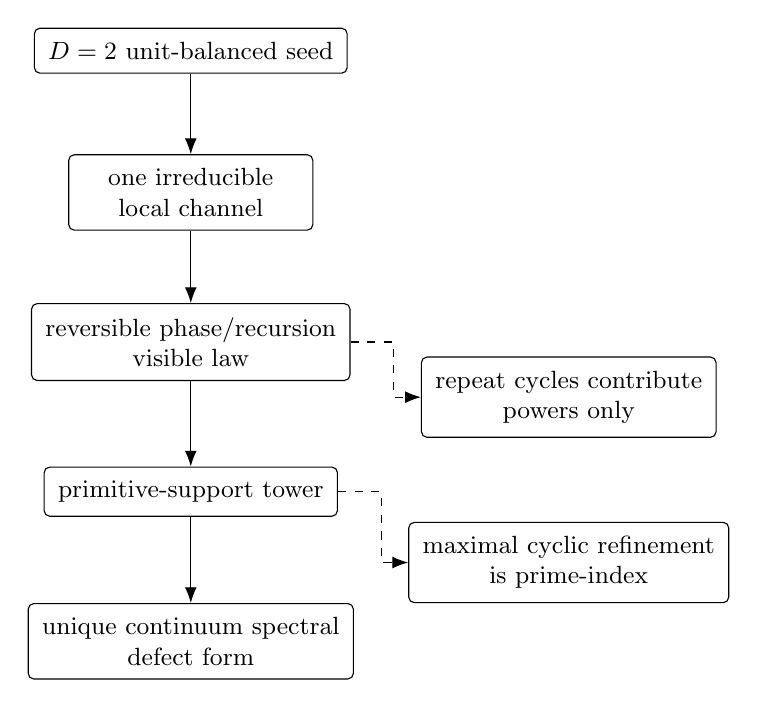
\begin{tikzpicture}[node distance=1.6cm]
  \node[ccbox, align=center, minimum width=3.0cm] (seed) at (0,1.8)
    {$D=2$ unit-balanced seed};
  \node[ccbox, align=center, minimum width=3.1cm] (channel) at (0,0.0)
    {one irreducible\\local channel};
  \node[ccbox, align=center, minimum width=3.2cm] (law) at (0,-1.9)
    {reversible phase/recursion\\visible law};
  \node[ccbox, align=center, minimum width=3.2cm] (support) at (0,-3.8)
    {primitive-support tower};
  \node[ccbox, align=center, minimum width=3.4cm] (continuum) at (0,-5.7)
    {unique continuum spectral\\defect form};

  \node[ccbox, align=center, minimum width=3.0cm] (repeat) at (4.8,-2.6)
    {repeat cycles contribute\\powers only};
  \node[ccbox, align=center, minimum width=3.0cm] (prime) at (4.8,-4.7)
    {maximal cyclic refinement\\is prime-index};

  \draw[ccarrow] (seed) -- (channel);
  \draw[ccarrow] (channel) -- (law);
  \draw[ccarrow] (law) -- (support);
  \draw[ccarrow] (support) -- (continuum);
  \draw[ccdarrow] (law.east) -- ++(0.55,0) |- (repeat.west);
  \draw[ccdarrow] (support.east) -- ++(0.55,0) |- (prime.west);
\end{tikzpicture}%
}
\caption{The \(D=2\) spectral seed. The one-channel seed forces a reversible
phase/recursion law; new spectral data arise only on primitive supports.}
\label{fig:d2-spectral-seed}
\end{figure}

This statement is operator-theoretic only: no arithmetic prime
identification is used. The \(D=2\) seed remains separate from the flagship
carrier class and furnishes the spectral stage beneath the nontrivial
\(D=4\) bundle.

Writing the forced continuum form as
\[
\mathcal E_{\infty}^{\mathrm{prim}},
\]
one natural external bridge problem is the identification
\[
\mathcal E_{\infty}^{\mathrm{prim}} = W_{\xi},
\]
where \(W_{\xi}\) denotes the classical completed Weil quadratic form on the
same log-time test class in Weil's positivity formulation of the explicit
formula \cite{Weil1952,Bombieri2000}. Any arithmetic realization of this
bridge would lie outside the operator calculus developed here. No such
identification is assumed here.

\subsubsection{Inherited Compatibility and Closure}

The flagship sections use these laws in five concrete representation
types. In each case, the carrier statement is proved inside the corresponding
section from the realized compatibility data, and the closure statement is the
inherited minimal-order closure mechanism already proved on the exported
structural interfaces.

\begin{remark}[Compatibility and order are inherited from the earlier structural interfaces]
\label{rem:compatibility-is-inherited}\lean{ObserverSelection.InheritedCompatibility}
No new compatibility identity is introduced at this stage. The compatibility
identities are already present in the exported theorem interfaces of
the earlier structural development and are only filtered by the selected
observer cut. Depending on
the realized family, these already include:
\begin{enumerate}[label=(\roman*), leftmargin=2em, itemsep=0.2em]
\item characteristic cut conservation and characteristic boundary reduction, by
      Theorem~\ref{thm:cut-conservation} and
      Corollary~\ref{cor:characteristic-boundary-reduction};
\item observer-side and dynamics-side triad compatibility, by
      Proposition~\ref{prop:observer-triad} and
      Theorem~\ref{thm:dynamics-triad};
\item reversible recursion and second-order wave transport on selected
      carriers, by
      Section~\ref{subsec:reversible-transport-recursion} together with the
      local datum-forcing interfaces cited in the wave and phase flagships;
\item nilpotent complex compatibility \(D_{k+1}D_k=0\) and the exactness/solver
      layer on finite Hilbert complexes, by
      Definition~\ref{def:hilbert-complex},
      Definition~\ref{def:exactness}, and
      Definition~\ref{def:solver-exactness};
\item local gauge covariance and unique gauge-compatible local datum on
      selected channels, by
      Corollary~\ref{cor:realized-local-gauge-covariance} and
      Theorem~\ref{thm:gauge-compatible-local-datum-forcing};
\item intrinsic symmetry scalarization on selected carriers, by
      Corollary~\ref{cor:realized-self-adjoint-scalarization} and
      Corollary~\ref{cor:realized-isotropic-symmetric-response-scalarization};
\item distinguished admissible minimal-order classes and their realized
      forcing, by
      Theorem~\ref{thm:minimal-admissible-transport-order},
      Corollary~\ref{cor:minimal-transport-order-controls-jet}, and
      Corollary~\ref{cor:realized-transport-order-forcing}; whenever a local
      representative family is later exhibited, Chapter~9 then verifies that
      representative by exact-core realization or constructive continuum
      forcing.
\end{enumerate}
Accordingly the later carrier sections ask only two questions: which inherited
compatibility identities are faithfully visible on the selected cut, and which
inherited minimal admissible closures preserve them there? Temporal
realization contributes the observer-side selection of the cut together with
the restriction that visible productions enter only as exact balanced
exchange.
\end{remark}

\subsubsection{Least-Motion Realization Data}

\begin{definition}[Characteristic observer datum]
\label{def:characteristic-observer-datum}\lean{ObserverSelection.CharacteristicDatum}
Fix a horizon \(h\), a characteristic horizon realization \(R\), and a
selection datum \(\mathsf S_h(R)\) in the sense of
Definition~\ref{def:selection-datum}. A \emph{characteristic observer datum}
at scale \(h\) consists of:
\begin{enumerate}[label=(\roman*), leftmargin=2em, itemsep=0.2em]
\item the selected horizon projector \(P_h\) and visible carrier
      \[
      \mathcal X_h:=P_h\cH^\bullet;
      \]
\item the lower-bound operator \(D_h\), candidate reduced-law family
      \(\mathcal Q_h(R)\), compatibility package, local-order filtration, and
      normalization package \(\mathcal N_h\) carried by \(\mathsf S_h(R)\);
\item the reconstruction and promotion data needed to place the selected family
      in the continuum-identification and admissible-promotion interfaces of
      the continuum bridge, together with the induced continuum carrier
      \(\mathcal X_{\chi^\ast}\) and continuum law space
      \(\mathcal Y_{\chi^\ast}\).
\end{enumerate}
\end{definition}

\begin{definition}[Least-motion characteristic observer]
\label{def:least-motion-characteristic-observer}\lean{ObserverSelection.LeastMotion}
A characteristic observer datum at scale \(h\) is a
\emph{least-motion characteristic observer} if:
\begin{enumerate}[label=(\roman*), leftmargin=2em, itemsep=0.2em]
\item it is faithful and reconstruction-compatible in the sense required by
      the continuum bridge;
\item it is closure-admissible, so the reduced admissible set
      \[
      \{Q\in\mathcal Q_h(R): D_h+Q\succeq 0\}
      \]
      is nonempty and well posed;
\item no proper visible subcarrier of \(\mathcal X_h\) still satisfies
      faithful reconstruction, compatibility preservation, and
      closure-admissibility;
\item its selected law class is stable under the admissible-promotion map of
      the continuum bridge;
\item among observer data satisfying (i)--(iv), it minimizes observer motion,
      meaning the combined representational drift of the projection, the
      minimal admissible completion, and the promoted law across the chosen
      horizon family;
\item it is unique up to horizon-preserving equivalence.
\end{enumerate}
\end{definition}

\begin{remark}[Triad consequence]
\label{rem:triad-consequence-observer-selection}\lean{ObserverSelection.TriadConsequence}
When a least-motion characteristic observer exists and is unique, the
Lagrangian/Eulerian/characteristic triad is read as a consequence of the
selected cut:
\[
\begin{aligned}
\Pi_{\chi^\ast}(\text{bulk-following description})
&=
\Pi_{\chi^\ast}(\text{boundary-observing description})\\
&=
\Pi_{\chi^\ast}(\text{action/generator description}).
\end{aligned}
\]
The surviving symmetry is then recovered as the stabilizer of the minimizing
observer datum rather than inserted by hand. In this sense, observer
covariance is the abstract symmetry statement, and the triad is its first
realized instance.
\end{remark}

\subsection{Common Structural Consequences}

\begin{theorem}[Common selected-bundle assembly]
\label{thm:common-selected-bundle-assembly}\lean{SelectedBundle.Assembly.surface}
Fix a realized family satisfying the temporal realization principle on a
least-motion characteristic observer datum with selected visible effective law
\(\mathcal L_{\mathrm{vis},h}(z)\). Assume that the phase, wave, kinetic,
gauge, and geometric intrinsic carriers together with the hydrodynamic balance
carrier on the selected cut are all faithful,
reconstruction-compatible, and stable under admissible promotion in the sense
of Definition~\ref{def:characteristic-observer-datum}.
Then:
\begin{enumerate}[label=(\roman*), leftmargin=2em, itemsep=0.2em]
\item these carriers are associated visible carriers of one selected observed
      bundle
      \[
      \mathcal X_h=P_h\cH^\bullet;
      \]
\item each induced visible law is obtained from the same selected
      visible effective law by restriction to the corresponding carrier
      together with the inherited selected endpoint closure class of
      Definition~\ref{def:selected-visible-effective-law};
\item once a canonical representative has been fixed on each carrier, the
      distinction between the flagship laws enters only at the final
      carrier-level endpoint classification and notation.
\end{enumerate}
\end{theorem}

(Proof in Appendix~\ref{sec:appendix-carrier}.)

\begin{theorem}[Common endpoint-rigidity reduction on the selected cut]
\label{thm:common-endpoint-rigidity-reduction}\lean{EndpointRigidity.CommonReduction.surface}
Fix a realized family satisfying the temporal realization principle on a
least-motion characteristic observer and an associated visible carrier
\(\mathcal X_h^{\mathrm{vis}}\) on the selected cut whose intrinsic symmetry
decomposition lies in the scalarization surfaces already forced upstream:
every non-geometric irreducible channel is an observable-irreducible selected
channel in the sense of
Definition~\ref{def:observable-irreducible-realized-class}, while every
geometric symmetric-response sector is an isotropic orthogonally equivariant
symmetric-tensor channel in the sense of
Corollary~\ref{cor:realized-isotropic-symmetric-response-scalarization}.
Then the selected endpoint closure class on
\(\mathcal X_h^{\mathrm{vis}}\) already has a unique exact carrier-side
representative, hence is unique modulo continuum equivalence, and is determined
entirely by scalar data on the intrinsic symmetry channels of that carrier.
Consequently the remaining carrier-level step is only to identify a natural
representative of that constructively forced class.
\end{theorem}

(Proof in Appendix~\ref{sec:appendix-carrier}.)


\manuscriptchapter{8}{The Intrinsic Carriers}
\section{Intrinsic Laws on the Selected Cut}
\label{sec:intrinsic-visible-laws}
This chapter treats the intrinsic visible laws whose leading form is already
fixed once the earlier carrier-forcing and endpoint-rigidity theorems are in
place: the three primitive channels (local-state, propagative, and
comparative) together with the canonical geometric lift of the primitive
\(3\)-channel. Their full physical reading is taken up in Part~II; here the
focus is the intrinsic carrier-level normal forms themselves rather than any
effective constitutive closure.
% ============================================================
\subsection{Local-State Persistence and Phase-Hamiltonian Realization}
\label{sec:flagship-quantum}
% ============================================================

The phase lane is the realization of \emph{local-state persistence}: a local
coherent state remains itself through the realized temporal order and carries a
reversible scalar transport law on the smallest faithful cut where that mode
is visible. Phase rigidity, transport rigidity, and scalar closure then
determine the physical phase law class on that realized cut using only the
interfaces inherited from the earlier structural chapters together with the
continuum bridge. The phase generator itself is forced
internally by phase generation and selected-cut energy orthogonality. The
recognizable Schr\"odinger form is obtained by local collapse of the already
forced transport/closure class to its canonical Laplace/potential
representative.

Theorem~\ref{thm:temporal-realization-forbids-primitive-internal-creation}
fixes the admissible source meaning on this carrier. In a closed reversible
phase sector there is no primitive visible creation, so any visible
inhomogeneity must appear as exchange with another visible sector or as
returned residual from the hidden complement on the same coherent bundle.

The relevant compatibility identity on this carrier is phase-compatible
reversible transport: the selected cut is the smallest one on which the forced
phase class, scalar recursive transport datum, and scalar closure class are
faithfully visible. The interval \(J\subseteq\bbR\) introduced below is
therefore not extra primitive data; it is a coordinate model of the realized
causal order on the phase carrier.

\paragraph{Carrier status.}
On the current theorem surface, the phase carrier itself is no longer being
introduced from scratch in this flagship section. By
Theorem~\ref{thm:three-forcing-bridges-from-bedrock-to-primitive-physics}, the
primitive direct lanes are already forced on the selected bundle. The
phase-Hamiltonian package below should therefore be read as the compatibility
and representative surface for the already forced \(1\)-channel, not as an
independent sectoral hypothesis beside the temporal realization law.

\subsubsection{Phase-Hamiltonian Realization}

\begin{definition}[Phase-Hamiltonian realization]
\label{def:phase-hamiltonian-realization}\lean{PhaseLane.HamiltonianRealization}
Let \(J\subseteq \bbR\) be a compact time interval, let \(\mathcal W\) be a
Hilbert space with dense test domain \(\mathcal W_0\subseteq\mathcal W\), and
let
\[
\mathcal F=\{(R_n,h_n,L_n)\}_{n\in\bbN}
\]
be a refinement-compatible realized law family into \(\mathcal W\). A
\emph{phase-Hamiltonian realization} on a visible carrier
\(\mathcal X_{\mathrm{ph}}\subseteq\mathcal W\) consists of:
\begin{enumerate}[label=(\roman*),itemsep=0.2em]
\item for every \(n\), the relevant selected channels of \(R_n\) carry
      selected channel transport systems and belong to admissible realized
      classes satisfying the hypotheses of
      Corollary~\ref{cor:intrinsic-package-implies-governing-datum-rigid};
\item the selected channel families are organized into a
      refinement-compatible family on \(C^1(J,\mathcal W_0)\) with a
      refinement-coherent reconstruction datum whose exact core realization is
      bounded;
\item the induced continuum transport class on \(\mathcal X_{\mathrm{ph}}\) is
      represented by a self-adjoint second-order operator
      \[
      \mathcal T_{\chi}:\mathcal W_0\to\mathcal W;
      \]
\item the induced continuum closure class on \(\mathcal X_{\mathrm{ph}}\) is
      represented by a self-adjoint scalar operator
      \[
      V_{\chi}:\mathcal W_0\to\mathcal W.
      \]
\end{enumerate}
\end{definition}

\subsubsection{Least-Motion Phase Carrier}

\begin{theorem}[Least-motion phase observer]
\label{thm:least-motion-phase-observer}\lean{PhaseLane.leastMotionObserver}
Assume the hypotheses of Definition~\ref{def:phase-hamiltonian-realization}.
Suppose:
\begin{enumerate}[label=(\roman*),itemsep=0.2em]
\item the phase carrier \(\mathcal X_{\mathrm{ph}}\) is faithful,
      closure-admissible, and stable under admissible promotion for the
      realized family;
\item no proper visible subcarrier of \(\mathcal X_{\mathrm{ph}}\) still
      supports a forced phase-carrier class, a scalar recursive transport
      datum, and a scalar closure class at the observed scale;
\item any characteristic observer datum satisfying \emph{(i)}--\emph{(ii)} is
      horizon-preserving equivalent to the datum generated by
      \(\mathcal X_{\mathrm{ph}}\).
\end{enumerate}
Then \(\mathcal X_{\mathrm{ph}}\) is the unique least-motion characteristic
observer for the realized family.
\end{theorem}

(Proof in Appendix~\ref{sec:appendix-carrier}.)

\subsubsection{Induced Reversible Phase Law}

\begin{theorem}[Induced reversible phase law on the selected cut]
\label{thm:induced-phase-hamiltonian-law}\lean{PhaseLane.inducedHamiltonianLaw}
Assume the hypotheses of
Theorem~\ref{thm:least-motion-phase-observer}. Then there exist a
representative \(J_{\chi}\) of the forced phase-carrier class on the selected
cut, a unique induced scalar coefficient \(\kappa_{\chi}\ge 0\), and a
remainder \(\mathsf R_{\mathrm{ph}}\in C(J,\mathcal W)\) such that every
\(\psi\in C^1(J,\mathcal W_0)\) satisfies
\[
J_{\chi}\partial_t\psi
=
\bigl(-\kappa_{\chi}\mathcal T_{\chi}+V_{\chi}\bigr)\psi
+
\mathsf R_{\mathrm{ph}}.
\]
By
Theorem~\ref{thm:temporal-realization-forbids-primitive-internal-creation},
\(\mathsf R_{\mathrm{ph}}\) is an exchange remainder rather than a primitive
source term on the selected cut.
If the selected cut is lossless at leading order, so that
\(\mathsf R_{\mathrm{ph}}=0\), this is the forced reversible phase law on the
selected cut.
\end{theorem}

(Proof in Appendix~\ref{sec:appendix-carrier}.)

The theorem above therefore reduces the phase lane to a carrier-level
representative problem. The selected cut already fixes the reversible phase law
class, the scalar transport coefficient, and the admissible exchange
remainder. The next theorem shows that the phase generator is internally
canonical on the selected cut; the local transport/closure collapse then
identifies the Laplace/potential representative.

\begin{theorem}[Phase generation and exact selected-cut energy split force the canonical complex generator]
\label{thm:phase-generation-and-energy-orthogonality-force-complex-generator}\lean{PhaseLane.EndpointFoundationFrontierData.complexGeneratorSurface}
Assume the hypotheses of
Theorem~\ref{thm:induced-phase-hamiltonian-law}. Assume in addition that, on
each relevant selected phase channel, the realized class on the selected cut
is phase-generated in the sense of
Definition~\ref{def:phase-generated-realized-class}, that the realized family
satisfies a canonical selected Schur bridge on that same selected cut. Then
the forced phase-carrier class on the selected cut admits a unique
pairing-compatible strong representative. In standard complex notation, that
representative is the canonical complex phase generator on
\(\mathcal X_{\mathrm{ph}}\).
\end{theorem}

(Proof in Appendix~\ref{sec:appendix-carrier}.)

\subsubsection{Endpoint Identification}

Writing the selected phase representative and transport datum in standard
wave-mechanics form now separates into two carrier-level steps. The phase
generator is already fixed by
Theorem~\ref{thm:phase-generation-and-energy-orthogonality-force-complex-generator}.
The final identification is the unique local pairing-symmetric
transport/closure representative on the selected cut. When that local endpoint
family assumes the standard Laplace/potential form, the resulting
endpoint law is the classical Schr\"odinger equation
\cite{Schrodinger1926,Stone1932}.

\begin{definition}[Phase local endpoint-rigidity package]
\label{def:phase-local-endpoint-rigidity-package}\lean{PhaseLane.EndpointCollapse}
Assume the hypotheses of
Theorem~\ref{thm:phase-generation-and-energy-orthogonality-force-complex-generator}.
A \emph{phase local endpoint-rigidity package} on the selected phase carrier
\(\mathcal X_{\mathrm{ph}}\) consists of:
\begin{enumerate}[label=(\roman*),itemsep=0.2em]
\item the minimal pairing-symmetric transport family on
      \(\mathcal X_{\mathrm{ph}}\) is represented levelwise by a
      refinement-compatible local scalar stencil family of minimal local order
      \(2\);
\item on each relevant selected phase channel, the corresponding one-step
      transport data are without preferred direction at quadratic order in the
      sense of
      Definition~\ref{def:no-preferred-direction-selected-channel-system};
\item the transport stencil family carries a refinement-coherent
      reconstruction datum on \((\mathcal W,\mathcal W_0)\) whose exact core
      realization is bounded;
\item the scalar closure family on \(\mathcal X_{\mathrm{ph}}\) is represented
      levelwise by a refinement-compatible local scalar stencil family of
      order \(0\);
\item the scalar closure family carries a refinement-coherent reconstruction
      datum on \((\mathcal W,\mathcal W_0)\) whose exact core realization is
      bounded.
\end{enumerate}
\end{definition}

\begin{theorem}[Phase local endpoint collapse to Laplace/potential form]
\label{thm:phase-local-endpoint-collapse}\lean{PhaseLane.endpointCollapse}
Assume the hypotheses of
Definition~\ref{def:phase-local-endpoint-rigidity-package}. Then there exist a
forced positive Laplace-type representative
\[
\Delta_{\chi}:\mathcal W_0\to\mathcal W
\]
for the selected transport class and a forced real multiplication operator
\[
V:\mathcal W_0\to\mathcal W
\]
for the selected scalar closure class such that every
\(\psi\in C^1(J,\mathcal W_0)\) satisfies
\[
i\,\partial_t\psi
=
\bigl(-\kappa_{\chi}\Delta_{\chi}+V\bigr)\psi
+
\mathsf R_{\mathrm{ph}}.
\]
If the selected cut is lossless at leading order, so that
\(\mathsf R_{\mathrm{ph}}=0\), this is exactly the Schr\"odinger equation on
the selected phase carrier.
\end{theorem}

(Proof in Appendix~\ref{sec:appendix-carrier}.)

\begin{corollary}[Recognizable Schr\"odinger identity]
\label{cor:recognizable-schrodinger-identity}\lean{PhaseLane.recognizableIdentity}
Assume the hypotheses of
Definition~\ref{def:phase-local-endpoint-rigidity-package}. Then the selected
phase carrier satisfies the Schr\"odinger identity
\[
i\,\partial_t\psi
=
\bigl(-\kappa_{\chi}\Delta_{\chi}+V\bigr)\psi
+
\mathsf R_{\mathrm{ph}},
\]
where \(\Delta_{\chi}\) is the forced positive Laplace-type transport
representative and \(V\) is the forced real multiplication potential. If the
selected cut is lossless at leading order, so that \(\mathsf R_{\mathrm{ph}}=0\),
this is exactly the Schr\"odinger equation on the selected carrier.
\end{corollary}

\begin{proof}
This is exactly Theorem~\ref{thm:phase-local-endpoint-collapse}.
\end{proof}

\begin{corollary}[Exact Schur form of the selected phase remainder]
\label{cor:phase-schur-remainder-identity}\lean{PhaseLane.schurRemainder}
Assume the hypotheses of
Theorem~\ref{thm:phase-local-endpoint-collapse}. Assume in addition that the
same selected datum satisfies a canonical selected Schur bridge. Then there is
a unique phase-projected Schur correction
\[
\Sigma_{h,\mathrm{ph}}(z)\in C(J,\mathcal W)
\]
obtained by reading the common selected Schur correction \(\CCSigma{h}{z}\)
through the forced phase endpoint identification on the selected carrier, and
\[
\mathsf R_{\mathrm{ph}}=\Sigma_{h,\mathrm{ph}}(z).
\]
Accordingly, every \(\psi\in C^1(J,\mathcal W_0)\) satisfies
\[
i\,\partial_t\psi
=
\bigl(-\kappa_{\chi}\Delta_{\chi}+V\bigr)\psi
+
\Sigma_{h,\mathrm{ph}}(z).
\]
\end{corollary}

(Proof in Appendix~\ref{sec:appendix-carrier}.)

\subsubsection{Concrete Hidden-Channel Phase Model}

The exact Schur form above becomes computationally informative once one
computes the returned phase profile on a concrete realized family. The
simplest solvable case is a visible phase carrier locally coupled to one
hidden phase carrier on the same primitive lattice. On that model the
phase remainder is an exact self-energy term in the usual spectral sense.

\begin{definition}[Coupled visible-shadow phase lattice model]
\label{def:coupled-visible-shadow-phase-lattice-model}\lean{PhaseLane.HiddenChannel.LatticeModel}
Assume the hypotheses of
Corollary~\ref{cor:phase-schur-remainder-identity}. A
\emph{coupled visible-shadow phase lattice model} consists of:
\begin{enumerate}[label=(\roman*),itemsep=0.2em]
\item a one-dimensional primitive lattice with spacing \(\ell_{\chi}>0\);
\item a visible lattice phase law
      \[
      i\,\partial_t\psi
      =
      \bigl(-\kappa_{\chi}\Delta_{\chi}+U_{\chi}\bigr)\psi
      +
      \gamma_{\chi}\eta,
      \]
      where
      \[
      (\Delta_{\chi}\psi)_n
      =
      \frac{\psi_{n+1}-2\psi_n+\psi_{n-1}}{\ell_{\chi}^2},
      \qquad
      U_{\chi}\in\bbR;
      \]
\item a hidden lattice phase law
      \[
      i\,\partial_t\eta
      =
      \bigl(-\widetilde\kappa_{\chi}\Delta_{\chi}+\widetilde U_{\chi}\bigr)\eta
      +
      \gamma_{\chi}\psi,
      \]
      with \(\widetilde\kappa_{\chi}\ge 0\),
      \(\widetilde U_{\chi}\in\bbR\), and \(\gamma_{\chi}\ge 0\);
\item a common selected plane-wave sector on which
      \[
      \psi_n(t)=\Psi\,e^{i(nk\ell_{\chi}-\omega t)},
      \qquad
      \eta_n(t)=H\,e^{i(nk\ell_{\chi}-\omega t)}
      \]
      for amplitudes \(\Psi,H\in\mathbb C\).
\end{enumerate}
\end{definition}

\begin{theorem}[Exact hidden-channel phase remainder and spectral splitting]
\label{thm:hidden-channel-phase-remainder-and-spectral-splitting}\lean{PhaseLane.HiddenChannel.splitting}
Assume the hypotheses of
Definition~\ref{def:coupled-visible-shadow-phase-lattice-model}. Define the
visible and hidden phase profiles
\[
E_{\mathrm{vis}}(k)
:=
U_{\chi}
+
\frac{4\kappa_{\chi}}{\ell_{\chi}^2}
\sin^2\!\left(\frac{k\ell_{\chi}}{2}\right),
\]
\[
E_{\mathrm{hid}}(k)
:=
\widetilde U_{\chi}
+
\frac{4\widetilde\kappa_{\chi}}{\ell_{\chi}^2}
\sin^2\!\left(\frac{k\ell_{\chi}}{2}\right).
\]
Then on every mode with \(E_{\mathrm{hid}}(k)\neq \omega\), exact elimination
of the hidden amplitude gives the returned phase profile
\[
\sigma_{\chi}^{\mathrm{ph,hid}}(k,\omega)
=
\frac{\gamma_{\chi}^2}{E_{\mathrm{hid}}(k)-\omega}.
\]
Accordingly the visible phase law is
\[
\omega
=
E_{\mathrm{vis}}(k)
+
\sigma_{\chi}^{\mathrm{ph,hid}}(k,\omega),
\]
equivalently
\[
(\omega-E_{\mathrm{vis}}(k))
(\omega-E_{\mathrm{hid}}(k))
=
\gamma_{\chi}^2.
\]
Hence the two exact mixed phase branches are
\[
\omega_{\pm}(k)
=
\frac{
E_{\mathrm{vis}}(k)+E_{\mathrm{hid}}(k)
\pm
\sqrt{
\bigl(E_{\mathrm{vis}}(k)-E_{\mathrm{hid}}(k)\bigr)^2
+
4\gamma_{\chi}^2
}
}{2}.
\]
\end{theorem}

(Proof in Appendix~\ref{sec:appendix-carrier}.)

\begin{corollary}[Exact off-resonant phase line shifts]
\label{cor:exact-off-resonant-phase-line-shifts}\lean{PhaseLane.HiddenChannel.offResonantShifts}
Assume the hypotheses of
Theorem~\ref{thm:hidden-channel-phase-remainder-and-spectral-splitting}. Define
\[
\delta_{\chi}^{\mathrm{ph}}(k):=E_{\mathrm{hid}}(k)-E_{\mathrm{vis}}(k).
\]
If \(\delta_{\chi}^{\mathrm{ph}}(k)>0\), then
\[
\omega_-(k)
=
E_{\mathrm{vis}}(k)
-
\frac{
2\gamma_{\chi}^2
}{
\delta_{\chi}^{\mathrm{ph}}(k)
+
\sqrt{
\bigl(\delta_{\chi}^{\mathrm{ph}}(k)\bigr)^2+4\gamma_{\chi}^2
}
},
\]
\[
\omega_+(k)
=
E_{\mathrm{hid}}(k)
+
\frac{
2\gamma_{\chi}^2
}{
\delta_{\chi}^{\mathrm{ph}}(k)
+
\sqrt{
\bigl(\delta_{\chi}^{\mathrm{ph}}(k)\bigr)^2+4\gamma_{\chi}^2
}
}.
\]
In particular, away from hidden resonance the visible-like phase branch is
shifted downward and the hidden-like branch upward.
\end{corollary}

(Proof in Appendix~\ref{sec:appendix-carrier}.)

\begin{corollary}[Exact avoided crossing of the coupled phase branches]
\label{cor:exact-avoided-crossing-coupled-phase-branches}\lean{PhaseLane.HiddenChannel.avoidedCrossing}
Assume the hypotheses of
Theorem~\ref{thm:hidden-channel-phase-remainder-and-spectral-splitting}. Suppose
there exists a selected mode \(k_\ast\) such that
\[
E_{\mathrm{vis}}(k_\ast)=E_{\mathrm{hid}}(k_\ast)=:E_\ast.
\]
Then
\[
\omega_{\pm}(k_\ast)=E_\ast\pm\gamma_{\chi},
\]
so the exact spectral gap at the would-be crossing is
\[
\omega_+(k_\ast)-\omega_-(k_\ast)=2\gamma_{\chi}.
\]
In particular, if \(\gamma_{\chi}>0\), the two phase branches do not cross.
\end{corollary}

(Proof in Appendix~\ref{sec:appendix-carrier}.)

\begin{corollary}[Low-energy renormalized phase offset and transport coefficient]
\label{cor:low-energy-renormalized-phase-offset-and-transport-coefficient}\lean{PhaseLane.HiddenChannel.lowEnergyRenormalization}
Assume the hypotheses of
Theorem~\ref{thm:hidden-channel-phase-remainder-and-spectral-splitting}. Define
\[
\Delta_0^{\mathrm{ph}}:=\widetilde U_{\chi}-U_{\chi},
\qquad
\Delta_1^{\mathrm{ph}}:=\widetilde\kappa_{\chi}-\kappa_{\chi},
\]
and assume \(\Delta_0^{\mathrm{ph}}>0\). Then as \(k\to 0\), the lower exact
phase branch has the expansion
\[
\omega_-(k)
=
U_{\chi,\mathrm{eff}}
+
\kappa_{\chi,\mathrm{eff}}\,k^2
+
O(k^4),
\]
where
\[
U_{\chi,\mathrm{eff}}
=
\frac{
U_{\chi}+\widetilde U_{\chi}
-
\sqrt{
\bigl(\Delta_0^{\mathrm{ph}}\bigr)^2+4\gamma_{\chi}^2
}
}{2},
\]
\[
\kappa_{\chi,\mathrm{eff}}
=
\frac{
\kappa_{\chi}+\widetilde\kappa_{\chi}
-
\frac{
\Delta_0^{\mathrm{ph}}\Delta_1^{\mathrm{ph}}
}{
\sqrt{
\bigl(\Delta_0^{\mathrm{ph}}\bigr)^2+4\gamma_{\chi}^2
}
}
}{2}.
\]
Thus hidden-channel return renormalizes both the phase offset and the long-wave
transport coefficient on the visible-like branch.
\end{corollary}

(Proof in Appendix~\ref{sec:appendix-carrier}.)

The two-channel phase model gives an exact coherent realization of the returned
phase profile. On this model, the remainder manifests as spectral line shifts,
avoided crossing, and low-energy renormalization of the visible phase offset
and transport coefficient. Irreversible decoherence would require a richer
hidden-sector family, such as a continuum or many-channel return model, and is
not part of the present two-channel calculation.

% ============================================================
\subsection{Propagative Persistence and Reversible Wave Realization}
\label{sec:flagship-wave}
% ============================================================

The wave lane is the realization of \emph{propagative persistence}: scalar
coherence remains visible by reversible spread through the realized temporal
order. The physical question on this lane is therefore how persistent scalar
coherence propagates on the time-realizing cut. Second-order transport
rigidity, scalar endpoint closure, and the continuum bridge then determine the
physical wave law class using only the machinery inherited from the earlier
structural chapters together with the continuum bridge.
The canonical wave form is obtained by identification of the local endpoint
representative inside that forced class. The exact
constant-mass Klein--Gordon specialization is a further refinement after that
local collapse, not part of the forcing of the wave representative itself.

Theorem~\ref{thm:temporal-realization-forbids-primitive-internal-creation}
again rules out primitive source creation on a closed reversible carrier. Any
visible inhomogeneity in the selected wave law must therefore be an exchange
remainder generated by coupling or hidden-sector return.

The relevant compatibility identity on this carrier is reversible second-order
transport: the selected cut is the smallest one on which the scalar wave
transport datum and scalar endpoint closure class are faithfully visible. The
interval \(J\subseteq\bbR\) introduced below is therefore a coordinate model of
the realized causal order on this carrier, not an extra primitive input.

\paragraph{Carrier status.}
The wave carrier itself is already fixed at the common-law level. By
Theorem~\ref{thm:three-forcing-bridges-from-bedrock-to-primitive-physics}, the
primitive direct lanes are already forced on the selected bundle, and the wave
lane is the canonical realization of the \(2\)-channel. The realization and
endpoint packages below are therefore compatibility/readout data for an
already forced lane, not an independent wave-sector axiom.

\subsubsection{Reversible Wave Realization}

\begin{definition}[Reversible wave realization]
\label{def:reversible-wave-realization}\lean{WaveLane.ReversibleRealization}
Let \(J\subseteq \bbR\) be a compact time interval, let \(\mathcal W\) be a
Hilbert space with dense test domain \(\mathcal W_0\subseteq\mathcal W\), and
let
\[
\mathcal F=\{(R_n,h_n,L_n)\}_{n\in\bbN}
\]
be a refinement-compatible realized law family into \(\mathcal W\). A
\emph{reversible wave realization} on a visible carrier
\(\mathcal X_{\mathrm{wav}}\subseteq\mathcal W\) consists of:
\begin{enumerate}[label=(\roman*),itemsep=0.2em]
\item for every \(n\), the relevant selected channels of \(R_n\) carry
      selected channel transport systems and belong to admissible realized
      classes satisfying the hypotheses of
      Corollary~\ref{cor:intrinsic-package-implies-governing-datum-rigid};
\item the selected channel families are organized into a
      refinement-compatible family on \(C^2(J,\mathcal W_0)\) with a
      refinement-coherent reconstruction datum whose exact core realization is
      bounded;
\item the induced continuum transport class on \(\mathcal X_{\mathrm{wav}}\)
      is represented by a self-adjoint nonnegative second-order operator
      \[
      \mathcal T_{\chi}:\mathcal W_0\to\mathcal W;
      \]
\item the induced continuum closure class on \(\mathcal X_{\mathrm{wav}}\) is
      represented by a self-adjoint scalar operator
      \[
      M_{\chi}:\mathcal W_0\to\mathcal W.
      \]
\end{enumerate}
\end{definition}

\subsubsection{Least-Motion Wave Carrier}

\begin{theorem}[Least-motion wave observer]
\label{thm:least-motion-wave-observer}\lean{WaveLane.leastMotionObserver}
Assume the hypotheses of Definition~\ref{def:reversible-wave-realization}.
Suppose:
\begin{enumerate}[label=(\roman*),itemsep=0.2em]
\item the wave carrier \(\mathcal X_{\mathrm{wav}}\) is faithful,
      closure-admissible, and stable under admissible promotion for the
      realized family;
\item no proper visible subcarrier of \(\mathcal X_{\mathrm{wav}}\) still
      supports a forced scalar second-order transport datum together with a
      scalar endpoint closure class at the observed scale;
\item any characteristic observer datum satisfying \emph{(i)}--\emph{(ii)} is
      horizon-preserving equivalent to the datum generated by
      \(\mathcal X_{\mathrm{wav}}\).
\end{enumerate}
Then \(\mathcal X_{\mathrm{wav}}\) is the unique least-motion characteristic
observer for the realized family.
\end{theorem}

(Proof in Appendix~\ref{sec:appendix-carrier}.)

\subsubsection{Induced Reversible Wave Law}

\begin{theorem}[Induced reversible wave law on the selected cut]
\label{thm:induced-wave-law}\lean{WaveLane.inducedLaw}
Assume the hypotheses of
Theorem~\ref{thm:least-motion-wave-observer}. Then there exist a unique induced
speed coefficient \(c_{\chi}>0\), a self-adjoint nonnegative transport operator
\(\mathcal T_{\chi}\), a self-adjoint scalar closure operator \(M_{\chi}\), and
a remainder \(\mathsf R_{\mathrm{wav}}\in C(J,\mathcal W)\) such that every
\(\phi\in C^2(J,\mathcal W_0)\) satisfies
\[
\partial_t^2\phi
+
c_{\chi}^2\mathcal T_{\chi}\phi
+
M_{\chi}\phi
=
\mathsf R_{\mathrm{wav}}.
\]
By
Theorem~\ref{thm:temporal-realization-forbids-primitive-internal-creation},
\(\mathsf R_{\mathrm{wav}}\) is an exchange remainder rather than an
independent source term.
If the selected cut is lossless at leading order, so that
\(\mathsf R_{\mathrm{wav}}=0\), this is the forced reversible wave law on the
selected cut.
\end{theorem}

(Proof in Appendix~\ref{sec:appendix-carrier}.)

The theorem above therefore reduces the wave lane to a local
representative-identification problem. The selected cut already fixes the
second-order transport operator, the scalar closure operator, and the
admissible exchange remainder. The canonical pairing-symmetric representative
of this forced class is then identified with the standard
wave/Laplace/scalar-profile operator. Once that identification is made, the
recognizable scalar wave identity follows; the exact Klein--Gordon
specialization is then the additional statement that the forced scalar profile
has a distinguished constant-mass part.

\subsubsection{Endpoint Identification and Wave Prediction}

In standard relativistic scalar notation, the recognized endpoint law is the
scalar wave equation with real scalar profile. Here again the final
identification is not a free notation choice: it is the local endpoint collapse
of the already forced wave class. The nearest-neighbor specialization below is
then the standard periodic-lattice dispersion law
\cite{Klein1926,Gordon1926,Brillouin1953}.

\begin{definition}[Wave local endpoint-rigidity package]
\label{def:wave-local-endpoint-rigidity-package}\lean{WaveLane.EndpointCollapse}
Assume the hypotheses of Theorem~\ref{thm:induced-wave-law}. A
\emph{wave local endpoint-rigidity package} on the selected wave carrier
\(\mathcal X_{\mathrm{wav}}\) consists of:
\begin{enumerate}[label=(\roman*),itemsep=0.2em]
\item the minimal pairing-symmetric transport family on
      \(\mathcal X_{\mathrm{wav}}\) is represented levelwise by a
      refinement-compatible local scalar stencil family of minimal local order
      \(2\);
\item on each relevant selected wave channel, the corresponding one-step
      transport data are without preferred direction at quadratic order in the
      sense of
      Definition~\ref{def:no-preferred-direction-selected-channel-system};
\item the transport stencil family carries a refinement-coherent
      reconstruction datum on \((\mathcal W,\mathcal W_0)\) whose exact core
      realization is bounded;
\item the scalar endpoint-closure family on \(\mathcal X_{\mathrm{wav}}\) is
      represented levelwise by a refinement-compatible local scalar stencil
      family of order \(0\);
\item the scalar closure family carries a refinement-coherent reconstruction
      datum on \((\mathcal W,\mathcal W_0)\) whose exact core realization is
      bounded.
\end{enumerate}
\end{definition}

\begin{theorem}[Wave local endpoint collapse to Laplace/scalar-profile form]
\label{thm:wave-local-endpoint-collapse}\lean{WaveLane.endpointCollapse}
Assume the hypotheses of
Definition~\ref{def:wave-local-endpoint-rigidity-package}. Then there exist a
forced positive Laplace-type representative
\[
\Delta_{\chi}:\mathcal W_0\to\mathcal W
\]
for the selected transport class and a forced real multiplication operator
\[
W_{\chi}:\mathcal W_0\to\mathcal W
\]
for the selected scalar closure class such that every
\(\phi\in C^2(J,\mathcal W_0)\) satisfies
\[
\partial_t^2\phi
-
c_{\chi}^2\Delta_{\chi}\phi
+
W_{\chi}\phi
=
\mathsf R_{\mathrm{wav}}.
\]
If the selected cut is lossless at leading order, so that
\(\mathsf R_{\mathrm{wav}}=0\), this is exactly the scalar wave equation on the
selected wave carrier.
\end{theorem}

(Proof in Appendix~\ref{sec:appendix-carrier}.)

\begin{corollary}[Recognizable wave/Klein--Gordon identity]
\label{cor:recognizable-wave-kg-identity}\lean{WaveLane.recognizableIdentity}
Assume the hypotheses of
Theorem~\ref{thm:wave-local-endpoint-collapse}. Assume in addition that the
forced real scalar closure profile on the selected carrier is written in the
form
\[
W_{\chi}=m_{\chi}^2+V
\]
for a nonnegative constant mass datum \(m_{\chi}^2\) and a real residual
potential \(V\). Then
\[
\partial_t^2\phi
-
c_{\chi}^2\Delta_{\chi}\phi
+
(m_{\chi}^2+V)\phi
=
\mathsf R_{\mathrm{wav}}.
\]
If the selected cut is lossless at leading order, so that
\(\mathsf R_{\mathrm{wav}}=0\), this is exactly the scalar wave identity on the
selected carrier, and when \(m_{\chi}\neq 0\) it is its Klein--Gordon form.
\end{corollary}

\begin{proof}
This is exactly Theorem~\ref{thm:wave-local-endpoint-collapse} after writing the
forced real multiplication profile \(W_{\chi}\) in the displayed
mass/potential form.
\end{proof}

\begin{corollary}[Exact Schur form of the selected wave remainder]
\label{cor:wave-schur-remainder-identity}\lean{WaveLane.schurRemainder}
Assume the hypotheses of Theorem~\ref{thm:wave-local-endpoint-collapse}. Assume
in addition that the same selected datum satisfies a canonical selected Schur
bridge. Then there is a unique wave-projected Schur correction
\[
\Sigma_{h,\mathrm{wav}}(z)\in C(J,\mathcal W)
\]
obtained by reading the common selected Schur correction \(\CCSigma{h}{z}\)
through the forced wave endpoint identification on the selected carrier, and
\[
\mathsf R_{\mathrm{wav}}=\Sigma_{h,\mathrm{wav}}(z).
\]
Accordingly, every \(\phi\in C^2(J,\mathcal W_0)\) satisfies
\[
\partial_t^2\phi
-
c_{\chi}^2\Delta_{\chi}\phi
+
W_{\chi}\phi
=
\Sigma_{h,\mathrm{wav}}(z).
\]
\end{corollary}

(Proof in Appendix~\ref{sec:appendix-carrier}.)

\begin{definition}[Homogeneous constant-mass wave refinement package]
\label{def:homogeneous-constant-mass-wave-refinement-package}\lean{WaveLane.ConstantMassRefinement}
Assume the hypotheses of
Theorem~\ref{thm:wave-local-endpoint-collapse}. A
\emph{homogeneous constant-mass wave refinement package} on the selected wave
carrier consists of:
\begin{enumerate}[label=(\roman*),itemsep=0.2em]
\item on each relevant selected wave channel, the admissible realized class
      furnishing the scalar closure profile is locally homogeneous on the
      selected channels in the sense of
      Definition~\ref{def:locally-homogeneous-realized-class};
\item the selected scalar closure family is equivariant for the induced local
      symmetry action on the corresponding homogeneous selected-wave sector;
\item after the wave local endpoint collapse, the forced zeroth-order closure
      profile on the selected wave carrier has no residual site-dependent
      scalar defect beyond that homogeneous selected-wave sector;
\item the resulting scalar closure is nonnegative on that homogeneous
      selected-wave sector.
\end{enumerate}
\end{definition}

\begin{theorem}[Homogeneous wave scalar profile forces exact constant mass]
\label{thm:homogeneous-wave-scalar-profile-forces-constant-mass}\lean{WaveLane.constantMass}
Assume the hypotheses of
Definition~\ref{def:homogeneous-constant-mass-wave-refinement-package}. Then
there exists a unique nonnegative constant mass datum \(m_{\chi}^2\in\bbR\)
such that
\[
W_{\chi}=m_{\chi}^2 I
\]
on the selected wave carrier. Consequently every
\(\phi\in C^2(J,\mathcal W_0)\) satisfies
\[
\partial_t^2\phi
-
c_{\chi}^2\Delta_{\chi}\phi
+
m_{\chi}^2\phi
=
\mathsf R_{\mathrm{wav}}.
\]
\end{theorem}

(Proof in Appendix~\ref{sec:appendix-carrier}.)

\begin{corollary}[Exact recognizable Klein--Gordon identity]
\label{cor:exact-recognizable-klein-gordon-identity}\lean{WaveLane.exactKleinGordon}
Assume the hypotheses of
Theorem~\ref{thm:homogeneous-wave-scalar-profile-forces-constant-mass}. Then
\[
\partial_t^2\phi
-
c_{\chi}^2\Delta_{\chi}\phi
+
m_{\chi}^2\phi
=
\mathsf R_{\mathrm{wav}}.
\]
If the selected cut is lossless at leading order, so that
\(\mathsf R_{\mathrm{wav}}=0\), this is exactly the constant-mass
Klein--Gordon equation on the selected wave carrier.
\end{corollary}

\begin{proof}
This is exactly
Theorem~\ref{thm:homogeneous-wave-scalar-profile-forces-constant-mass} read in
the standard Klein--Gordon notation.
\end{proof}

\begin{definition}[Nearest-neighbor wave specialization]
\label{def:nearest-neighbor-wave-specialization}\lean{WaveLane.NearestNeighborSpecialization}
Assume the hypotheses of
Theorem~\ref{thm:induced-wave-law}. A \emph{nearest-neighbor wave
specialization} of the selected cut consists of:
\begin{enumerate}[label=(\roman*),itemsep=0.2em]
\item a one-dimensional primitive lattice with spacing \(\ell_{\chi}>0\);
\item the lossless massless leading-order regime
      \[
      M_{\chi}=0,
      \qquad
      \mathsf R_{\mathrm{wav}}=0;
      \]
\item the selected transport operator acting by the second-difference law
      \[
      (\mathcal T_{\chi}\phi)_n
      =
      \frac{2\phi_n-\phi_{n+1}-\phi_{n-1}}{\ell_{\chi}^2}.
      \]
\end{enumerate}
\end{definition}

\begin{theorem}[Exact lattice dispersion on the selected wave carrier]
\label{thm:exact-wave-dispersion}\lean{WaveLane.exactDispersion}
Assume the hypotheses of
Definition~\ref{def:nearest-neighbor-wave-specialization}. Then plane-wave
modes
\[
\phi_n(t)=e^{i(nk\ell_{\chi}-\omega t)}
\]
satisfy
\[
\omega(k)^2
=
\frac{4c_{\chi}^2}{\ell_{\chi}^2}
\sin^2\!\left(\frac{k\ell_{\chi}}{2}\right),
\]
and, writing \(E=\hbar\omega\) and \(E_{\chi}:=\hbar c_{\chi}/\ell_{\chi}\),
the corresponding group velocity is
\[
v_g(E)
=
c_{\chi}\sqrt{1-\left(\frac{E}{2E_{\chi}}\right)^2}
\qquad (0\le E\le 2E_{\chi}).
\]
\end{theorem}

(Proof in Appendix~\ref{sec:appendix-carrier}.)

\begin{corollary}[Observable wave-carrier signature]
\label{cor:observable-wave-carrier-signature}\lean{WaveLane.observableCarrierSignature}
Assume the hypotheses of
Theorem~\ref{thm:exact-wave-dispersion}. Then in the low-energy regime
\(E\ll E_{\chi}\),
\[
\frac{\delta v}{c_{\chi}}
=
\frac{v_g(E)-c_{\chi}}{c_{\chi}}
\approx
-\frac18\left(\frac{E}{E_{\chi}}\right)^2.
\]
In particular, the sign is fixed and subluminal, and the selected wave carrier
also predicts a hard cutoff at \(E=2E_{\chi}\), where \(v_g(E)\) collapses to
zero.
\end{corollary}

(Proof in Appendix~\ref{sec:appendix-carrier}.)

\subsubsection{Schur-Corrected Lattice Dispersion}

The lossless nearest-neighbor law isolates the clean leading wave surface.
To read the predictive remainder without weakening that identification, keep
the same lattice transport and constant-mass closure but allow the exact
returned Schur correction to survive on a single selected plane-wave sector.
On such a sector the returned wave remainder is read as a scalar correction to
the dispersion relation, not as a new primitive law.

\begin{definition}[Mode-compatible Schur-corrected lattice-wave specialization]
\label{def:mode-compatible-schur-corrected-lattice-wave-specialization}\lean{WaveLane.CorrectedDispersion.LatticeSpecialization}
Assume the hypotheses of
Corollary~\ref{cor:wave-schur-remainder-identity} and
Theorem~\ref{thm:homogeneous-wave-scalar-profile-forces-constant-mass}. A
\emph{mode-compatible Schur-corrected lattice-wave specialization} of the
selected cut consists of:
\begin{enumerate}[label=(\roman*),itemsep=0.2em]
\item a one-dimensional primitive lattice with spacing \(\ell_{\chi}>0\);
\item the selected Laplace-type transport representative acting by the
      second-difference law
      \[
      (\Delta_{\chi}\phi)_n
      =
      \frac{\phi_{n+1}-2\phi_n+\phi_{n-1}}{\ell_{\chi}^2};
      \]
\item the selected scalar closure being the constant-mass operator
      \[
      W_{\chi}=m_{\chi}^2 I
      \qquad (m_{\chi}\ge 0);
      \]
\item a selected plane-wave sector generated by
      \[
      \phi_n(t)=e^{i(nk\ell_{\chi}-\omega t)};
      \]
\item the exact returned wave remainder being mode-compatible and time-local on
      that sector, in the sense that there exists a real scalar correction
      profile \(\sigma_{\chi}(k;z)\) such that
      \[
      \Sigma_{h,\mathrm{wav}}(z)_n(t)
      =
      \sigma_{\chi}(k;z)\,\phi_n(t)
      \]
      for every mode in the selected sector.
\end{enumerate}
\end{definition}

\begin{theorem}[Exact Schur-corrected lattice dispersion on the selected wave carrier]
\label{thm:exact-schur-corrected-wave-dispersion}\lean{WaveLane.CorrectedDispersion.laws}
Assume the hypotheses of
Definition~\ref{def:mode-compatible-schur-corrected-lattice-wave-specialization}.
Then the selected plane-wave sector satisfies the exact corrected dispersion law
\[
\omega(k;z)^2
=
m_{\chi}^2
+
\frac{4c_{\chi}^2}{\ell_{\chi}^2}
\sin^2\!\left(\frac{k\ell_{\chi}}{2}\right)
-
\sigma_{\chi}(k;z).
\]
If in addition \(k\mapsto \sigma_{\chi}(k;z)\) is differentiable and the
displayed right-hand side is positive, then the corresponding group velocity is
\[
v_g(k;z)
=
\frac{
\frac{2c_{\chi}^2}{\ell_{\chi}}\sin(k\ell_{\chi})
-\partial_k\sigma_{\chi}(k;z)
}{
2\sqrt{
m_{\chi}^2
+
\frac{4c_{\chi}^2}{\ell_{\chi}^2}
\sin^2\!\left(\frac{k\ell_{\chi}}{2}\right)
-
\sigma_{\chi}(k;z)
}
}.
\]
When \(\sigma_{\chi}(k;z)=0\), this reduces to the lossless lattice law of
Theorem~\ref{thm:exact-wave-dispersion}; when \(m_{\chi}=0\), it further
reduces to the massless signature of
Corollary~\ref{cor:observable-wave-carrier-signature}.
\end{theorem}

(Proof in Appendix~\ref{sec:appendix-carrier}.)

This theorem gives an exact non-lossless wave specialization on the selected
plane-wave sector. Once a concrete realized family yields a returned profile
\(\sigma_{\chi}(k;z)\), the observed dispersion and group velocity are fixed
by the displayed formulas. The lossless lattice law is recovered as the
special case \(\sigma_{\chi}(k;z)=0\).

\subsubsection{Concrete Hidden-Channel Model}

The abstract corrected profile \(\sigma_{\chi}(k;z)\) becomes more informative
once one computes it on a concrete realized family. The simplest exactly
solvable model is a visible lattice wave locally coupled to one hidden lattice
wave on the same selected primitive lattice. In that case the returned
remainder is a genuine wave-side self-energy induced by exact elimination of
the hidden channel.

\begin{definition}[Coupled visible-shadow lattice-wave model]
\label{def:coupled-visible-shadow-lattice-wave-model}\lean{WaveLane.HiddenChannel.LatticeModel}
Assume the hypotheses of
Definition~\ref{def:mode-compatible-schur-corrected-lattice-wave-specialization}.
A \emph{coupled visible-shadow lattice-wave model} consists of:
\begin{enumerate}[label=(\roman*),itemsep=0.2em]
\item a hidden scalar lattice field \(\eta_n(t)\) on the same one-dimensional
      lattice of spacing \(\ell_{\chi}\);
\item a hidden nearest-neighbor wave operator with parameters
      \(\widetilde c_{\chi}>0\) and \(\widetilde m_{\chi}\ge 0\), acting by
      \[
      \partial_t^2\eta
      -
      \widetilde c_{\chi}^2\Delta_{\chi}\eta
      +
      \widetilde m_{\chi}^2\eta;
      \]
\item a real local coupling amplitude \(\gamma_{\chi}\ge 0\) such that the
      visible and hidden fields satisfy
      \[
      \partial_t^2\phi
      -
      c_{\chi}^2\Delta_{\chi}\phi
      +
      m_{\chi}^2\phi
      =
      \gamma_{\chi}\eta,
      \]
      \[
      \partial_t^2\eta
      -
      \widetilde c_{\chi}^2\Delta_{\chi}\eta
      +
      \widetilde m_{\chi}^2\eta
      =
      \gamma_{\chi}\phi;
      \]
\item a common plane-wave sector on which
      \[
      \phi_n(t)=\Phi\,e^{i(nk\ell_{\chi}-\omega t)},
      \qquad
      \eta_n(t)=H\,e^{i(nk\ell_{\chi}-\omega t)}
      \]
      for amplitudes \(\Phi,H\in\mathbb C\).
\end{enumerate}
\end{definition}

\begin{theorem}[Exact hidden-channel wave remainder and branch splitting]
\label{thm:hidden-channel-wave-remainder-and-branch-splitting}\lean{WaveLane.HiddenChannel.splitting}
Assume the hypotheses of
Definition~\ref{def:coupled-visible-shadow-lattice-wave-model}. Define the
visible and hidden leading profiles
\[
\omega_{\mathrm{vis}}(k)^2
:=
m_{\chi}^2
+
\frac{4c_{\chi}^2}{\ell_{\chi}^2}
\sin^2\!\left(\frac{k\ell_{\chi}}{2}\right),
\]
\[
\omega_{\mathrm{hid}}(k)^2
:=
\widetilde m_{\chi}^2
+
\frac{4\widetilde c_{\chi}^2}{\ell_{\chi}^2}
\sin^2\!\left(\frac{k\ell_{\chi}}{2}\right).
\]
Then on every mode with \(\omega_{\mathrm{hid}}(k)^2\neq \omega^2\), exact
elimination of the hidden amplitude gives the returned wave profile
\[
\sigma_{\chi}^{\mathrm{hid}}(k,\omega)
=
\frac{\gamma_{\chi}^2}{\omega_{\mathrm{hid}}(k)^2-\omega^2}.
\]
Accordingly the visible dispersion law is
\[
\omega^2
=
\omega_{\mathrm{vis}}(k)^2
-
\sigma_{\chi}^{\mathrm{hid}}(k,\omega),
\]
equivalently
\[
(\omega^2-\omega_{\mathrm{vis}}(k)^2)
(\omega^2-\omega_{\mathrm{hid}}(k)^2)
=
\gamma_{\chi}^2.
\]
Hence the two exact propagating branches are
\[
\omega_{\pm}(k)^2
=
\frac{
\omega_{\mathrm{vis}}(k)^2+\omega_{\mathrm{hid}}(k)^2
\pm
\sqrt{
\bigl(\omega_{\mathrm{vis}}(k)^2-\omega_{\mathrm{hid}}(k)^2\bigr)^2
+
4\gamma_{\chi}^2
}
}{2}.
\]
\end{theorem}

(Proof in Appendix~\ref{sec:appendix-carrier}.)

\begin{corollary}[Exact off-resonant branch shifts]
\label{cor:exact-off-resonant-hidden-channel-branch-shifts}\lean{WaveLane.HiddenChannel.offResonantShifts}
Assume the hypotheses of
Theorem~\ref{thm:hidden-channel-wave-remainder-and-branch-splitting}. Define
\[
\delta_{\chi}(k)
:=
\omega_{\mathrm{hid}}(k)^2-\omega_{\mathrm{vis}}(k)^2.
\]
If \(\delta_{\chi}(k)>0\) for a selected mode \(k\), then the two exact
branches satisfy
\[
\omega_-(k)^2
=
\omega_{\mathrm{vis}}(k)^2
-
\frac{2\gamma_{\chi}^2}{
\delta_{\chi}(k)+\sqrt{\delta_{\chi}(k)^2+4\gamma_{\chi}^2}
},
\]
\[
\omega_+(k)^2
=
\omega_{\mathrm{hid}}(k)^2
+
\frac{2\gamma_{\chi}^2}{
\delta_{\chi}(k)+\sqrt{\delta_{\chi}(k)^2+4\gamma_{\chi}^2}
}.
\]
In particular, away from hidden resonance the visible-like branch is shifted
downward and the hidden-like branch is shifted upward by the same exact
returned remainder amplitude.
\end{corollary}

(Proof in Appendix~\ref{sec:appendix-carrier}.)

\begin{corollary}[Exact avoided crossing of the coupled wave branches]
\label{cor:exact-avoided-crossing-coupled-wave-branches}\lean{WaveLane.HiddenChannel.avoidedCrossing}
Assume the hypotheses of
Theorem~\ref{thm:hidden-channel-wave-remainder-and-branch-splitting}. Suppose
there exists a selected mode \(k_\ast\) such that
\[
\omega_{\mathrm{vis}}(k_\ast)^2
=
\omega_{\mathrm{hid}}(k_\ast)^2
=:
\omega_\ast^2.
\]
Then
\[
\omega_{\pm}(k_\ast)^2=\omega_\ast^2\pm\gamma_{\chi},
\]
so the squared-frequency gap at the would-be crossing is exactly
\[
\omega_+(k_\ast)^2-\omega_-(k_\ast)^2=2\gamma_{\chi}.
\]
In particular, if \(\gamma_{\chi}>0\), the two branches do not cross.
\end{corollary}

(Proof in Appendix~\ref{sec:appendix-carrier}.)

\begin{corollary}[Low-energy renormalized mass and wave speed]
\label{cor:low-energy-renormalized-mass-and-wave-speed-hidden-channel}\lean{WaveLane.HiddenChannel.lowEnergyRenormalization}
Assume the hypotheses of
Theorem~\ref{thm:hidden-channel-wave-remainder-and-branch-splitting}. Define
\[
\Delta_0:=\widetilde m_{\chi}^2-m_{\chi}^2,
\qquad
\Delta_1:=\widetilde c_{\chi}^2-c_{\chi}^2,
\]
and assume \(\Delta_0>0\). Then as \(k\to 0\), the lower exact branch has the
expansion
\[
\omega_-(k)^2
=
m_{\chi,\mathrm{eff}}^2
+
c_{\chi,\mathrm{eff}}^2\,k^2
+
O(k^4),
\]
where
\[
m_{\chi,\mathrm{eff}}^2
=
\frac{
m_{\chi}^2+\widetilde m_{\chi}^2
-\sqrt{\Delta_0^2+4\gamma_{\chi}^2}
}{2},
\]
\[
c_{\chi,\mathrm{eff}}^2
=
\frac{
c_{\chi}^2+\widetilde c_{\chi}^2
-\frac{\Delta_0\Delta_1}{\sqrt{\Delta_0^2+4\gamma_{\chi}^2}}
}{2}.
\]
Thus hidden-channel return renormalizes both the visible mass gap and the
long-wave propagation speed on the selected visible-like branch.
\end{corollary}

(Proof in Appendix~\ref{sec:appendix-carrier}.)

These corollaries identify the observable content of the solved hidden-channel
wave model. The returned wave remainder shifts the visible branch away from
resonance, opens an avoided crossing at resonance, and renormalizes the
effective mass gap and long-wave propagation speed at low energy.

% ============================================================
\subsection{Comparative Persistence and Gauge-Curvature Realization}
\label{sec:flagship-gauge}
% ============================================================

The gauge lane is the realization of \emph{comparative persistence}: only the
local comparison class is physically visible, and coherent exchange persists as
visible curvature and current. Exactness, local gauge covariance, and
inherited minimal-order closure then determine the physical
curvature/exchange law class on that carrier. The final carrier-level
identification of the canonical representative is completed below by local
endpoint rigidity on the selected one-form carrier.

Theorem~\ref{thm:temporal-realization-forbids-primitive-internal-creation}
identifies admissible one-form sources on that cut as visible exchange
currents rather than primitive creations.

The relevant compatibility identity on this carrier is nilpotent exactness:
closed curvature is inherited from the complex law \(d^2=0\) already built in
the earlier structural chapters together with the continuum bridge. The
spacetime slab \(M=J\times\Sigma\) introduced below is a
coordinate model of the realized temporal cut, with \(J\) carrying the
realized causal order.

\paragraph{Carrier status.}
The one-form carrier is likewise not being postulated independently here. By
Theorem~\ref{thm:three-forcing-bridges-from-bedrock-to-primitive-physics}, the
primitive direct lanes are already forced on the selected bundle, and the
gauge lane is the canonical realization of the \(3\)-channel. The role of the
present flagship section is to identify the gauge-compatible local datum and
its canonical representative, not to add a new sector law beside the temporal
realization principle.

\subsubsection{Gauge-Compatible Realization}

\begin{definition}[Gauge-compatible one-form realization]
\label{def:gauge-compatible-one-form-realization}\lean{GaugeLane.OneFormRealization}
Let \(M=J\times\Sigma\) be an oriented pseudo-Riemannian spacetime slab with
exterior derivative \(d\) and codifferential \(\delta\) induced by the Hodge
star of the chosen metric. A
\emph{gauge-compatible one-form realization} consists of:
\begin{enumerate}[label=(\roman*),itemsep=0.2em]
\item a visible carrier of local one-form classes \([A]\in\Omega^1(M)/d\Omega^0(M)\);
\item an exchange one-form \(J\in\Omega^1(M)\) satisfying
      \[
      \delta J=0;
      \]
\item the compatibility package given by exactness
      \[
      d^2=0,
      \]
      local gauge covariance under \(A\mapsto A+d\chi\), and continuum
      equivalence modulo local gauge;
\item the realized class is transport-order disciplined on the selected
      one-form carrier, and its distinguished admissible minimal-order class
      is local order \(2\) in \(A\), hence local order \(1\) in the
      transported curvature \(F:=dA\).
\end{enumerate}
\end{definition}

The codifferential \(\delta\) therefore depends on the metric/Hodge data on
\(M\); it is not determined by orientation alone.

\subsubsection{Least-Motion Gauge Carrier}

\begin{theorem}[Least-motion gauge observer]
\label{thm:least-motion-gauge-observer}\lean{GaugeLane.leastMotionObserver}
Assume the hypotheses of
Definition~\ref{def:gauge-compatible-one-form-realization}. Suppose:
\begin{enumerate}[label=(\roman*),itemsep=0.2em]
\item the realized family satisfies the hypotheses of
      Corollary~\ref{cor:intrinsic-package-yields-gauge-compatible-local-datum},
      so the selected law already carries a unique gauge-compatible local
      internal datum on the relevant selected channels;
\item the one-form carrier is faithful, closure-admissible, and stable under
      admissible promotion for the realized family;
\item no proper visible subcarrier still supports gauge-covariant,
      exactness-compatible exchange response together with faithful
      reconstruction and stable promotion at the observed scale;
\item any characteristic observer datum satisfying \emph{(i)}--\emph{(iii)} is
      horizon-preserving equivalent to the one generated by the selected
      one-form carrier.
\end{enumerate}
Then the selected one-form carrier is the unique least-motion characteristic
observer for the realized family.
\end{theorem}

(Proof in Appendix~\ref{sec:appendix-carrier}.)

\begin{definition}[Gauge-compatible curvature/exchange datum]
\label{def:gauge-compatible-curvature-source-datum}\lean{GaugeLane.CurvatureSourceDatum}
Assume the hypotheses of
Theorem~\ref{thm:least-motion-gauge-observer}. The
\emph{gauge-compatible curvature/exchange datum} on the selected cut is the
triple
\[
\mathfrak M_{\mathrm g}:=([A],F,J),
\qquad
F:=dA,
\]
where \([A]\) is the selected local gauge class on the one-form carrier and
\(J\) is the selected visible exchange current on that same cut.
\end{definition}

\subsubsection{Induced Curvature/Source Law}

\begin{theorem}[Induced gauge-compatible law on the selected cut]
\label{thm:induced-gauge-compatible-law}\lean{GaugeLane.inducedLaw}
Assume the hypotheses of
Theorem~\ref{thm:least-motion-gauge-observer}. Let
\(\mathfrak M_{\mathrm g}=([A],F,J)\) be the selected
gauge-compatible curvature/exchange datum of
Definition~\ref{def:gauge-compatible-curvature-source-datum}. Then there are a
unique gauge-compatible local response operator
\[
\mathcal M_{\mathrm g}:\Omega^1(M)/d\Omega^0(M)\to\Omega^1(M)
\]
of minimal local order and a local gauge-invariant remainder
\(\mathsf R_{\mathrm g}\in\Omega^1(M)\) such that
\[
dF=0,
\qquad
\mathcal M_{\mathrm g}([A])=J+\mathsf R_{\mathrm g}.
\]
Here \(J\) is the selected visible exchange current, and
Theorem~\ref{thm:temporal-realization-forbids-primitive-internal-creation}
identifies \(\mathsf R_{\mathrm g}\) as the remaining local gauge-invariant
exchange remainder on the selected cut.
If the selected cut is lossless at leading order, so that
\(\mathsf R_{\mathrm g}=0\), this is the forced gauge-compatible law on the
selected cut.
\end{theorem}

(Proof in Appendix~\ref{sec:appendix-carrier}.)

Thus the gauge carrier is already reduced to a local representative problem on
the selected cut: identify the canonical gauge-compatible representative
inside the forced curvature/exchange closure class. The local collapse below
first identifies the intrinsic selected-cut curvature-adjoint representative;
the recognizable Maxwell notation is then a downstream Hodge-side readout of
that already forced representative.

\subsubsection{Endpoint Identification}

In differential-form notation, the recognized endpoint law is the classical
Maxwell curvature/source system \cite{Maxwell1865}. The final response
operator is now read through a final local rigidity step. Exactness and local
gauge covariance already reduce the response from the gauge class \([A]\) to
the curvature \(F=dA\). The final identification is the unique
pairing-compatible first-order curvature representative on the selected cut.
When the generated one-form carrier is read on an energy-orthogonal realized
cut with its Hodge-side duality structure fixed, that representative is the
codifferential-curvature response.

\begin{definition}[Gauge local endpoint-rigidity package]
\label{def:gauge-local-endpoint-rigidity-package}\lean{GaugeLane.EndpointCollapse}
Assume the hypotheses of Theorem~\ref{thm:induced-gauge-compatible-law}. A
\emph{gauge local endpoint-rigidity package} on the selected one-form carrier
consists of:
\begin{enumerate}[label=(\roman*),itemsep=0.2em]
\item the realized family satisfies a canonical selected Schur bridge on that
      same selected cut;
\item the minimal pairing-symmetric response family on the selected one-form
      carrier is represented levelwise by a refinement-compatible local
      gauge-covariant stencil family of minimal local order \(2\) in \(A\),
      hence local order \(1\) in the curvature \(F=dA\);
\item the distinguished minimal-order response family on the selected one-form
      carrier carries a refinement-coherent reconstruction datum on its dense
      test domain whose exact core realization is bounded.
\end{enumerate}
\end{definition}

\begin{theorem}[Gauge local endpoint collapse to the canonical curvature-adjoint form]
\label{thm:gauge-local-endpoint-collapse}\lean{GaugeLane.endpointCollapse}
Assume the hypotheses of
Definition~\ref{def:gauge-local-endpoint-rigidity-package}. Then the forced
gauge-compatible endpoint class on the selected carrier has the canonical
curvature-adjoint representative
\[
\mathcal M_{\mathrm g}([A])=\delta_{\chi} dA=\delta_{\chi}F,
\]
where \(\delta_{\chi}\) denotes the adjoint of \(d\) with respect to the
canonical selected-cut pairing on the selected one-form carrier. Hence
\[
dF=0,
\qquad
\delta_{\chi}F=J+\mathsf R_{\mathrm g}.
\]
If the selected cut is lossless at leading order, so that
\(\mathsf R_{\mathrm g}=0\), this is the lossless intrinsic gauge law on the
selected one-form carrier.
\end{theorem}

(Proof in Appendix~\ref{sec:appendix-carrier}.)

\begin{corollary}[Recognizable Maxwell identity]
\label{cor:recognizable-maxwell-identity}\lean{GaugeLane.recognizableIdentity}
Assume the hypotheses of
Theorem~\ref{thm:gauge-local-endpoint-collapse}. Assume in addition that the
generated one-form carrier carries the canonical Hodge-side duality induced by
the chosen metric on \(M\), so the selected-cut adjoint \(\delta_{\chi}\) is
read as the codifferential \(\delta\).
Then
\[
dF=0,
\qquad
\delta F=J+\mathsf R_{\mathrm g}.
\]
If the selected cut is lossless at leading order, so that
\(\mathsf R_{\mathrm g}=0\), this is exactly the Maxwell curvature/source law,
with \(J\) recognized as the visible exchange current.
\end{corollary}

\begin{proof}
Substitute the Hodge-side identification \(\delta_{\chi}=\delta\) into
Theorem~\ref{thm:gauge-local-endpoint-collapse}.
\end{proof}

\begin{corollary}[Exact Schur form of the selected gauge remainder]
\label{cor:gauge-schur-remainder-identity}\lean{GaugeLane.schurRemainder}
Assume the hypotheses of
Theorem~\ref{thm:gauge-local-endpoint-collapse}. Assume in addition that the
same selected datum satisfies a canonical selected Schur bridge. Then there is
a unique gauge-projected Schur correction
\[
\Sigma_{h,\mathrm g}(z)\in\Omega^1(M)
\]
obtained by reading the common selected Schur correction \(\CCSigma{h}{z}\)
through the forced gauge endpoint identification on the selected carrier, and
\[
\mathsf R_{\mathrm g}=\Sigma_{h,\mathrm g}(z).
\]
Accordingly,
\[
dF=0,
\qquad
\delta_{\chi}F=J+\Sigma_{h,\mathrm g}(z).
\]
\end{corollary}

(Proof in Appendix~\ref{sec:appendix-carrier}.)

\subsubsection{Concrete Hidden-Channel Gauge Model}

The exact Schur form above becomes computationally informative once one
computes the returned gauge current on a concrete realized family. The
simplest solvable case is a transverse visible gauge mode locally coupled to
one hidden conserved current mode on the same primitive lattice. On that
model the gauge remainder is an exact current-side self-energy.

\begin{definition}[Coupled visible-shadow gauge mode model]
\label{def:coupled-visible-shadow-gauge-mode-model}\lean{GaugeLane.HiddenChannel.LatticeModel}
Assume the hypotheses of
Corollary~\ref{cor:gauge-schur-remainder-identity}. A
\emph{coupled visible-shadow gauge mode model} consists of:
\begin{enumerate}[label=(\roman*),itemsep=0.2em]
\item a one-dimensional primitive lattice with spacing \(\ell_{\chi}>0\)
      and a fixed transverse polarization one-form \(\varepsilon\);
\item a selected visible gauge mode and external visible current
      \[
      A_n(t)=a\,\varepsilon\,e^{i(nk\ell_{\chi}-\omega t)},
      \qquad
      J_n^{\mathrm{ext}}(t)=j_0\,\varepsilon\,e^{i(nk\ell_{\chi}-\omega t)};
      \]
\item a hidden transverse current mode
      \[
      B_n(t)=b\,\varepsilon\,e^{i(nk\ell_{\chi}-\omega t)};
      \]
\item visible and hidden spectral profiles
      \[
      \Omega_{\mathrm{g,vis}}(k)^2
      :=
      \frac{4c_{\chi}^2}{\ell_{\chi}^2}
      \sin^2\!\left(\frac{k\ell_{\chi}}{2}\right),
      \]
      \[
      \Omega_{\mathrm{g,hid}}(k)^2
      :=
      \nu_{\chi}^2
      +
      \frac{4\widetilde c_{\chi}^2}{\ell_{\chi}^2}
      \sin^2\!\left(\frac{k\ell_{\chi}}{2}\right),
      \]
      where \(c_{\chi}>0\), \(\widetilde c_{\chi}>0\), \(\nu_{\chi}\ge 0\),
      and \(\gamma_{\chi}\ge 0\);
\item a local coupling on the selected transverse sector such that the visible
      and hidden mode amplitudes satisfy
      \[
      \bigl(\Omega_{\mathrm{g,vis}}(k)^2-\omega^2\bigr)a
      =
      j_0+\gamma_{\chi}b,
      \]
      \[
      \bigl(\Omega_{\mathrm{g,hid}}(k)^2-\omega^2\bigr)b
      =
      \gamma_{\chi}a.
      \]
\end{enumerate}
\end{definition}

\begin{theorem}[Exact hidden-channel gauge current and branch splitting]
\label{thm:hidden-channel-gauge-current-and-branch-splitting}\lean{GaugeLane.HiddenChannel.splitting}
Assume the hypotheses of
Definition~\ref{def:coupled-visible-shadow-gauge-mode-model}. Then on every
mode with \(\Omega_{\mathrm{g,hid}}(k)^2\neq\omega^2\), exact elimination of
the hidden current amplitude gives the returned gauge current profile
\[
\sigma_{\chi}^{\mathrm{g,hid}}(k,\omega)
=
\frac{\gamma_{\chi}^2}{
\Omega_{\mathrm{g,hid}}(k)^2-\omega^2
}.
\]
Accordingly the visible response law is
\[
\bigl(\Omega_{\mathrm{g,vis}}(k)^2-\omega^2\bigr)a
=
j_0+\sigma_{\chi}^{\mathrm{g,hid}}(k,\omega)\,a,
\]
so the returned one-form remainder on that sector is
\[
\Sigma_{h,\mathrm g}^{\mathrm{hid}}(k,\omega)
=
\sigma_{\chi}^{\mathrm{g,hid}}(k,\omega)\,
a\,\varepsilon\,e^{i(nk\ell_{\chi}-\omega t)}.
\]
If \(j_0=0\), then
\[
(\omega^2-\Omega_{\mathrm{g,vis}}(k)^2)
(\omega^2-\Omega_{\mathrm{g,hid}}(k)^2)
=
\gamma_{\chi}^2,
\]
and the two exact mixed gauge branches are
\[
\omega_{\pm}(k)^2
=
\frac{
\Omega_{\mathrm{g,vis}}(k)^2+\Omega_{\mathrm{g,hid}}(k)^2
\pm
\sqrt{
\bigl(\Omega_{\mathrm{g,vis}}(k)^2-\Omega_{\mathrm{g,hid}}(k)^2\bigr)^2
+
4\gamma_{\chi}^2
}
}{2}.
\]
\end{theorem}

(Proof in Appendix~\ref{sec:appendix-carrier}.)

\begin{corollary}[Exact off-resonant gauge pole shifts]
\label{cor:exact-off-resonant-gauge-pole-shifts}\lean{GaugeLane.HiddenChannel.offResonantShifts}
Assume the hypotheses of
Theorem~\ref{thm:hidden-channel-gauge-current-and-branch-splitting} and
\(j_0=0\). Define
\[
\delta_{\chi}^{\mathrm g}(k)
:=
\Omega_{\mathrm{g,hid}}(k)^2-\Omega_{\mathrm{g,vis}}(k)^2.
\]
If \(\delta_{\chi}^{\mathrm g}(k)>0\), then
\[
\omega_-(k)^2
=
\Omega_{\mathrm{g,vis}}(k)^2
-
\frac{2\gamma_{\chi}^2}{
\delta_{\chi}^{\mathrm g}(k)
+
\sqrt{
\bigl(\delta_{\chi}^{\mathrm g}(k)\bigr)^2+4\gamma_{\chi}^2
}
},
\]
\[
\omega_+(k)^2
=
\Omega_{\mathrm{g,hid}}(k)^2
+
\frac{2\gamma_{\chi}^2}{
\delta_{\chi}^{\mathrm g}(k)
+
\sqrt{
\bigl(\delta_{\chi}^{\mathrm g}(k)\bigr)^2+4\gamma_{\chi}^2
}
}.
\]
In particular, away from hidden resonance the visible-like gauge pole is
shifted downward and the hidden current pole upward.
\end{corollary}

(Proof in Appendix~\ref{sec:appendix-carrier}.)

\begin{corollary}[Exact avoided crossing of the coupled gauge branches]
\label{cor:exact-avoided-crossing-coupled-gauge-branches}\lean{GaugeLane.HiddenChannel.avoidedCrossing}
Assume the hypotheses of
Theorem~\ref{thm:hidden-channel-gauge-current-and-branch-splitting} and
\(j_0=0\). Suppose there exists a selected mode \(k_\ast\) such that
\[
\Omega_{\mathrm{g,vis}}(k_\ast)^2
=
\Omega_{\mathrm{g,hid}}(k_\ast)^2
=:
\Omega_{\ast}^2.
\]
Then
\[
\omega_{\pm}(k_\ast)^2=\Omega_{\ast}^2\pm\gamma_{\chi},
\]
so the squared-frequency gap at the would-be crossing is exactly
\[
\omega_+(k_\ast)^2-\omega_-(k_\ast)^2=2\gamma_{\chi}.
\]
In particular, if \(\gamma_{\chi}>0\), the two gauge branches do not cross.
\end{corollary}

(Proof in Appendix~\ref{sec:appendix-carrier}.)

\begin{corollary}[Low-frequency induced exchange susceptibility]
\label{cor:low-frequency-induced-exchange-susceptibility}\lean{GaugeLane.HiddenChannel.lowFrequencySusceptibility}
Assume the hypotheses of
Theorem~\ref{thm:hidden-channel-gauge-current-and-branch-splitting} and
\(\nu_{\chi}>0\). Then as \((k,\omega)\to(0,0)\),
\[
\sigma_{\chi}^{\mathrm{g,hid}}(k,\omega)
=
\frac{\gamma_{\chi}^2}{\nu_{\chi}^2}
-
\frac{\gamma_{\chi}^2\widetilde c_{\chi}^2}{\nu_{\chi}^4}k^2
+
\frac{\gamma_{\chi}^2}{\nu_{\chi}^4}\omega^2
+
O(k^4+k^2\omega^2+\omega^4).
\]
Thus on the long-wave low-frequency sector the hidden return acts as an
induced local exchange susceptibility with static amplitude
\(\gamma_{\chi}^2/\nu_{\chi}^2\) together with the first dispersive
corrections.
\end{corollary}

(Proof in Appendix~\ref{sec:appendix-carrier}.)

The two-channel gauge model gives an exact realization of the returned gauge
current. On this model, the remainder manifests as gauge-pole shifts, avoided
crossing, and low-frequency induced exchange susceptibility on the visible
gauge sector.

\subsubsection{Exact Euclidean gauge shadow-flow}

The returned gauge correction admits an exact determinant-flow formulation
that is native to the tower calculus and structurally distinct from perturbative
running. This is the monograph's intrinsic exact gauge response law.

\begin{definition}[Selected gauge shadow-flow]
\label{def:selected-gauge-shadow-flow}\lean{GaugeLane.SelectedGaugeShadowFlow}
Assume the selected cut carries an intrinsic selected gauge carrier
$\mathcal Y_{h,\mathrm g}\subseteq \mathcal X_h$, and assume
$\mathcal Y_{h,\mathrm g}$ is finite-dimensional.
Let $P_{h,\mathrm g}:\mathcal X_h\to \mathcal Y_{h,\mathrm g}$ be the
orthogonal projection onto that carrier.

Let $T_h$ be the shadow-transport operator of
Definition~\ref{def:shadow-transport-invariants}. Define the
\emph{gauge shadow-transport compression} by
\[
T_{h,\mathrm g}
:=
P_{h,\mathrm g}\,T_h\,P_{h,\mathrm g}\big|_{\mathcal Y_{h,\mathrm g}}.
\]

Define the associated determinant flow and exact Euclidean gauge
shadow-flow by
\[
\Delta_{h,\mathrm g}(t):=\det(I+tT_{h,\mathrm g}),
\qquad
\tau_{h,\mathrm g}(t):=\frac{d}{dt}\log \Delta_{h,\mathrm g}(t),
\qquad t\ge 0.
\]
\end{definition}

\begin{theorem}[Exact Euclidean gauge shadow-flow law]
\label{thm:exact-euclidean-gauge-shadow-flow}\lean{GaugeLane.exactEuclideanGaugeShadowFlow}
Assume Definition~\ref{def:selected-gauge-shadow-flow}. Then:

\begin{enumerate}[label=\textup{(\roman*)}]
\item $T_{h,\mathrm g}$ is positive semidefinite.

\item If
$\Lambda_{h,\mathrm g}
=\{\lambda_{h,1},\dots,\lambda_{h,r_h}\}$
is the multiset of eigenvalues of $T_{h,\mathrm g}$ with multiplicity,
then
\[
\Delta_{h,\mathrm g}(t)=\prod_{j=1}^{r_h}(1+t\lambda_{h,j}),
\]
and
\[
\tau_{h,\mathrm g}(t)
=
\sum_{j=1}^{r_h}\frac{\lambda_{h,j}}{1+t\lambda_{h,j}}
=
\Tr\!\bigl(T_{h,\mathrm g}(I+tT_{h,\mathrm g})^{-1}\bigr).
\]

\item For every $n\ge 0$ and every $t\ge 0$,
\[
(-1)^n \tau_{h,\mathrm g}^{(n)}(t)
=
n!\,
\Tr\!\Bigl(
T_{h,\mathrm g}^{\,n+1}(I+tT_{h,\mathrm g})^{-(n+1)}
\Bigr)
\ge 0.
\]
Hence $\tau_{h,\mathrm g}$ is positive, decreasing, and completely
monotone on $[0,\infty)$.

\item If $\|tT_{h,\mathrm g}\|<1$, then
\[
\tau_{h,\mathrm g}(t)
=
\sum_{m=0}^{\infty}(-1)^m M_{m+1}^{(\mathrm g)}(h)\,t^m,
\]
where $M_k^{(\mathrm g)}(h):=\Tr(T_{h,\mathrm g}^k)$.

\item Let $E_{h,\mathrm g}$ be the spectral measure of $T_{h,\mathrm g}$,
and define the finite positive Borel measure
$\nu_{h,\mathrm g}(B)
:=\Tr\!\bigl(E_{h,\mathrm g}(B)\,T_{h,\mathrm g}\bigr)$.
Then
\[
\tau_{h,\mathrm g}(t)
=
\int_{[0,\infty)} \frac{1}{1+t\lambda}\,d\nu_{h,\mathrm g}(\lambda).
\]
In particular, $\tau_{h,\mathrm g}$ is a Stieltjes function.

\item $\tau_{h,\mathrm g}$ determines $\Delta_{h,\mathrm g}$ by
\[
\Delta_{h,\mathrm g}(t)
=
\exp\!\Bigl(\int_0^t \tau_{h,\mathrm g}(s)\,ds\Bigr),
\qquad
\Delta_{h,\mathrm g}(0)=1,
\]
and therefore determines the full spectral multiset
$\Lambda_{h,\mathrm g}$ and all moments $M_k^{(\mathrm g)}(h)$.
\end{enumerate}
\end{theorem}

\begin{proof}
Since $T_h$ is positive semidefinite by
Definition~\ref{def:shadow-transport-invariants}, its orthogonal
compression $T_{h,\mathrm g}=P_{h,\mathrm g}T_hP_{h,\mathrm g}$ is also
positive semidefinite: for every $u\in\mathcal Y_{h,\mathrm g}$,
$\langle u,T_{h,\mathrm g}u\rangle
=\langle P_{h,\mathrm g}u,T_hP_{h,\mathrm g}u\rangle
=\langle u,T_hu\rangle\ge 0$.
This proves~(i).

Because $\mathcal Y_{h,\mathrm g}$ is finite-dimensional and
$T_{h,\mathrm g}$ is self-adjoint, there is an orthonormal basis in which
$T_{h,\mathrm g}$ is diagonal with nonneg\-ative entries
$\lambda_{h,1},\dots,\lambda_{h,r_h}$. Therefore
$\Delta_{h,\mathrm g}(t)=\prod_j(1+t\lambda_{h,j})$.
Differentiating $\log\Delta_{h,\mathrm g}$ gives
$\tau_{h,\mathrm g}(t)=\sum_j\lambda_{h,j}/(1+t\lambda_{h,j})$.
The trace identity follows from the diagonal form of
$T_{h,\mathrm g}(I+tT_{h,\mathrm g})^{-1}$.
This proves~(ii).

Termwise differentiation yields
$\tau_{h,\mathrm g}^{(n)}(t)
=(-1)^n n!\sum_j\lambda_{h,j}^{n+1}/(1+t\lambda_{h,j})^{n+1}$,
which equals
$(-1)^n n!\,\Tr(T_{h,\mathrm g}^{n+1}(I+tT_{h,\mathrm g})^{-(n+1)})$.
Each summand is nonneg\-ative since $\lambda_{h,j}\ge 0$ and
$1+t\lambda_{h,j}>0$. Complete monotonicity follows.
This proves~(iii).

The geometric expansion
$\lambda_j/(1+t\lambda_j)=\sum_{m\ge 0}(-1)^m\lambda_j^{m+1}t^m$
converges absolutely for $|t\lambda_j|<1$. Summing over~$j$ gives the
moment series with $M_k^{(\mathrm g)}(h)=\sum_j\lambda_{h,j}^k$.
This proves~(iv).

By functional calculus,
$T_{h,\mathrm g}(I+tT_{h,\mathrm g})^{-1}
=\int\frac{\lambda}{1+t\lambda}\,dE_{h,\mathrm g}(\lambda)$.
Taking traces gives
$\tau_{h,\mathrm g}(t)=\int(1+t\lambda)^{-1}\,d\nu_{h,\mathrm g}(\lambda)$
with $\nu_{h,\mathrm g}$ positive (since $E_{h,\mathrm g}$ and
$T_{h,\mathrm g}$ are positive). This proves~(v).

Part~(vi) follows from $\Delta_{h,\mathrm g}(t)
=\exp(\int_0^t\tau_{h,\mathrm g}(s)\,ds)$ and the fact that the
characteristic polynomial $\prod_j(1+t\lambda_{h,j})$ determines the
eigenvalue multiset $\Lambda_{h,\mathrm g}$ and hence all moments.
\end{proof}

\begin{corollary}[Finite-horizon nonlogarithmic distinctness]
\label{cor:finite-horizon-nonlogarithmic-distinctness}\lean{GaugeLane.finiteHorizonNonlogarithmicDistinctness}
At every fixed horizon~$h$, the exact gauge shadow-flow
$\tau_{h,\mathrm g}(t)$ is a rational Stieltjes function of~$t$,
with simple poles only at the negative real numbers
$-\lambda_{h,j}^{-1}$ corresponding to the nonzero eigenvalues of
$T_{h,\mathrm g}$. In particular, the monograph-native exact law is not
logarithmic at finite resolution. Any logarithmic running can arise only
after passage to a continuum spectral limit of the measures
$\nu_{h,\mathrm g}$.
\end{corollary}

\begin{proof}
By Theorem~\ref{thm:exact-euclidean-gauge-shadow-flow}(ii),
$\tau_{h,\mathrm g}(t)=\sum_j\lambda_{h,j}/(1+t\lambda_{h,j})$
is rational with the stated poles. A rational function is not logarithmic.
\end{proof}

\begin{theorem}[Spectral-limit gauge shadow-flow]
\label{thm:spectral-limit-gauge-shadow-flow}\lean{GaugeLane.spectralLimitGaugeShadowFlow}
Assume a sequence of horizons $h_n$ such that the finite positive measures
$\nu_{h_n,\mathrm g}$ of
Theorem~\ref{thm:exact-euclidean-gauge-shadow-flow}(v) converge weakly to
a finite positive Borel measure $\nu_{\mathrm g}$ on $[0,\infty)$.
Define
\[
\tau_{\mathrm g}(t)
:=
\int_{[0,\infty)}\frac{1}{1+t\lambda}\,d\nu_{\mathrm g}(\lambda),
\qquad t\ge 0.
\]
Then for every $t\ge 0$,
$\tau_{h_n,\mathrm g}(t)\to \tau_{\mathrm g}(t)$.
\end{theorem}

\begin{proof}
For each fixed $t\ge 0$, the kernel $f_t(\lambda)=(1+t\lambda)^{-1}$
is bounded and continuous on $[0,\infty)$. By weak convergence,
$\int f_t\,d\nu_{h_n,\mathrm g}\to\int f_t\,d\nu_{\mathrm g}$.
By Theorem~\ref{thm:exact-euclidean-gauge-shadow-flow}(v), the left side
is $\tau_{h_n,\mathrm g}(t)$ and the right is $\tau_{\mathrm g}(t)$.
\end{proof}

% ============================================================
\subsection{Causal-Structural Persistence and Geometric Realization}
\label{sec:flagship-geometry}
% ============================================================

The geometric lane is the realization of \emph{causal-structural persistence}:
the causal order itself persists visibly by symmetric response to prior
exchange. The geometric question is therefore how coherent visible exchange
deforms the symmetric response carrier on the realized cut. Characteristic
endpoint reduction and intrinsic symmetry then determine the physical
geometric response law class using the inherited machinery of the earlier
structural chapters together with the continuum bridge. The
final carrier-level identification of the canonical representative is
completed below by local endpoint rigidity on the selected symmetric-tensor
carrier.

Theorem~\ref{thm:temporal-realization-forbids-primitive-internal-creation}
identifies the visible symmetric source term as balanced exchange with
preceding selected carriers rather than primitive creation. In this sense the
geometric lane is kept on the intrinsic side of Part~II: any constitutive
closure issue belongs to the preceding sector furnishing the exchange tensor
\(T\), not to the Einstein-side geometric response law itself.

The relevant compatibility identity on this carrier is covariant divergence
compatibility: the selected cut is the smallest one on which that tensor-side
compatibility law is faithfully visible.

\paragraph{Carrier status.}
Geometry is not introduced here as a fourth primitive sector. By
Theorems~\ref{thm:geometry-unique-lift-of-primitive-three-channel} and
\ref{thm:geometric-symmetric-square-factorization}, together with
\ref{thm:three-forcing-bridges-from-bedrock-to-primitive-physics}, the
geometric lane is already forced on the selected bundle as the unique
symmetric-response lift of the primitive \(3\)-channel. The local endpoint
package below should therefore be read as the final compatibility and
representative collapse on an already forced carrier class.

\subsubsection{Weak-Field Geometric Response}

\begin{definition}[Weak-field geometric response data]
\label{def:weak-field-symmetric-response-branch}\lean{GeometricLane.WeakFieldResponseData}
Let \(T\) be a symmetric exchange field furnished by a preceding selected law. A
\emph{weak-field geometric response datum} consists of:
\begin{enumerate}[label=(\roman*),itemsep=0.2em]
\item an observable carrier consisting of symmetric \(2\)-tensor fields \(h\);
\item an admissible local response class on that carrier whose leading order is
      second order, self-adjoint, and divergence-compatible, with the
      corresponding realized class transport-order disciplined on the selected
      symmetric-tensor carrier;
\item a leading response that is orthogonally equivariant on the
      symmetric tensor carrier, so the carrier has no preferred direction at
      the linear response level;
\item quadratic and higher response terms subordinate to the leading
      linear response.
\end{enumerate}
\end{definition}

\subsubsection{Least-Motion Geometric Carrier}

\begin{theorem}[Least-motion geometric observer]
\label{thm:least-motion-geometric-observer}\lean{GeometricLane.leastMotionObserver}
Assume the hypotheses of
Definition~\ref{def:weak-field-symmetric-response-branch}. Suppose:
\begin{enumerate}[label=(\roman*),itemsep=0.2em]
\item the symmetric \(2\)-tensor carrier is faithful, closure-admissible, and
      stable under admissible promotion for the promoted source/transport
      family;
\item no proper visible subcarrier still supports a faithful
      divergence-compatible second-order response law at the observed scale;
\item any characteristic observer datum satisfying \emph{(i)}--\emph{(ii)} is
      horizon-preserving equivalent to the symmetric \(2\)-tensor carrier.
\end{enumerate}
Then the symmetric \(2\)-tensor carrier is the unique least-motion
characteristic observer for the promoted source/transport family.
\end{theorem}

(Proof in Appendix~\ref{sec:appendix-carrier}.)

\subsubsection{Induced Weak-Field Law}

\begin{theorem}[Induced weak-field geometric law]
\label{thm:weak-field-geometric-response-law}\lean{GeometricLane.weakFieldLaw}
Assume the hypotheses of
Theorem~\ref{thm:least-motion-geometric-observer}. Then there are
induced scalar coefficients \(\Lambda_{\mathrm{ind}},\kappa_{\mathrm{ind}}\), a
unique divergence-compatible leading response operator
\(\mathcal E_{\mathrm{lin}}\) on symmetric \(2\)-tensor fields, and a
higher-order remainder \(\mathsf R_{\mathrm{grav}}\) such that
\[
\mathcal E_{\mathrm{lin}}(h)+\Lambda_{\mathrm{ind}}h
=
\kappa_{\mathrm{ind}}T+\mathsf R_{\mathrm{grav}}.
\]
If \(\mathsf R_{\mathrm{grav}}=0\), this is the forced weak-field law on the
selected cut.
\end{theorem}

(Proof in Appendix~\ref{sec:appendix-carrier}.)

\subsubsection{Covariant Completion and Induced Law}

\begin{remark}[Nonlinear completion locus]
\label{rem:nonlinear-completion-locus}\lean{GeometricLane.NonlinearCompletionLocus}
Up to this point, the geometric derivation is carrier forcing plus endpoint
reduction. The nonlinear step concerns classification of the admissible
minimal-order covariant completion class on the selected carrier rather than
selection of the carrier itself. The earlier structural chapters together with
the temporal
realization principle and its universal clauses reduce the nonlinear geometric
problem to that classification question.
\end{remark}

\begin{theorem}[Forced covariant geometric law on the selected cut]
\label{thm:characteristic-covariant-geometric-reduction}\lean{GeometricLane.covariantReduction}
Assume the hypotheses of
Theorem~\ref{thm:least-motion-geometric-observer}. Assume moreover:
\begin{enumerate}[label=(\roman*),itemsep=0.2em]
\item the exchange field \(T\) is divergence-compatible at the observed scale;
\item for each spacetime point \((x,t)\), with \(\Gamma_{x,t}\) the realized
      characteristic congruence through \((x,t)\), there is a rapidly decaying
      covariant memory family \(\mathcal M_{x,t}(s)\) on \(s\le 0\) such that
      the nonlinear correction admits the representation
      \[
      \mathcal N_{\mathrm{geom}}(x,t)
      =
      \int_{-\infty}^0
      \mathcal M_{x,t}(s)\bigl[
      \mathsf C(g,T)(\Gamma_{x,t}(s),t+s)
      \bigr]\,ds
      \]
      for a local symmetric curvature/exchange datum \(\mathsf C(g,T)\);
\item the bulk part of this characteristic integral reduces to endpoint data by
      Corollary~\ref{cor:characteristic-boundary-reduction};
\item on the decay scale of \(\mathcal M_{x,t}\), the geometric fields vary
      slowly enough that the characteristic integral admits a first-order
      endpoint expansion;
\item the induced endpoint map is covariant, divergence-compatible, and has no
      preferred transverse direction on the symmetric tensor carrier.
\item the admissible covariant completion class on the selected carrier is
      filtered by local differential order, its distinguished admissible order
      is \(2\), and the selected response operator lies in that minimal-order
      class.
\end{enumerate}
Then there are induced scalar coefficients
\(\Lambda_{\mathrm{ind}},\kappa_{\mathrm{ind}}\), a covariant
divergence-compatible response operator \(\mathcal G(g)\) of minimal local
order, and a local symmetric remainder \(\mathsf N_{\mathrm{grav}}(g,T)\) such
that
\[
\mathcal G(g)+\Lambda_{\mathrm{ind}}g
=
\kappa_{\mathrm{ind}}T+\mathsf N_{\mathrm{grav}}(g,T),
\qquad
\nabla^\mu\bigl(\mathcal G_{\mu\nu}(g)+\Lambda_{\mathrm{ind}}g_{\mu\nu}\bigr)=0.
\]
If the characteristic endpoint reduction is lossless at leading order, so that
\(\mathsf N_{\mathrm{grav}}=0\), this is the forced covariant law on the
selected cut.
\end{theorem}

(Proof in Appendix~\ref{sec:appendix-carrier}.)

\begin{remark}[Characteristic-return mechanism]
\label{rem:characteristic-path-origin-of-geometric-response}\lean{GeometricLane.CharacteristicReturnOrigin}
Theorem~\ref{thm:characteristic-covariant-geometric-reduction} is the symmetric
\(2\)-tensor analogue of Theorem~\ref{cor:hydrodynamic-closure-law}. The
nonlinear response is not inserted as an independent constitutive tensor. It is
carried by characteristic return, its bulk part cancels, and the surviving
endpoint map is forced onto the trace and traceless channels of the least-motion
observed carrier.
\end{remark}

Thus the geometric carrier is already reduced to a local representative
problem on the selected cut: identify the canonical divergence-compatible
representative inside the forced geometric closure class. The local collapse
below first identifies the intrinsic selected-cut trace-adjusted curvature
representative; the recognizable Einstein notation is then a downstream
Levi-Civita/Bianchi readout of that already forced representative.

\subsubsection{Endpoint Identification}

In standard covariant notation, the recognized endpoint law is the Einstein
equation with cosmological term \cite{Einstein1915,Wald1984}. On this carrier
the last representative identification is likewise a local endpoint-rigidity
statement. Once the selected symmetric-tensor carrier is read on an
energy-orthogonal realized cut and the canonical Levi-Civita/Bianchi-side
covariant duality is fixed there, the intrinsic trace-adjusted curvature
representative is read as the trace-adjusted Ricci / Einstein one.

\begin{definition}[Geometric local endpoint-rigidity package]
\label{def:geometric-local-endpoint-rigidity-package}\lean{GeometricLane.EndpointCollapse}
Assume the hypotheses of
Theorem~\ref{thm:characteristic-covariant-geometric-reduction}. A
\emph{geometric local endpoint-rigidity package} on the selected
symmetric-tensor carrier consists of:
\begin{enumerate}[label=(\roman*),itemsep=0.2em]
\item the realized family satisfies a canonical selected Schur bridge on that
      same selected cut;
\item the minimal covariant response family on the selected symmetric-tensor
      carrier is represented levelwise by a refinement-compatible local
      symmetric-tensor differential family of minimal local order \(2\);
\item the minimal covariant response family carries a
      refinement-coherent reconstruction datum on its dense test domain whose
      exact core realization is bounded.
\end{enumerate}
\end{definition}

\begin{theorem}[Geometric local endpoint collapse to the canonical trace-adjusted curvature form]
\label{thm:geometric-local-endpoint-collapse}\lean{GeometricLane.endpointCollapse}
Assume the hypotheses of
Definition~\ref{def:geometric-local-endpoint-rigidity-package}. Then the forced
geometric endpoint class on the selected symmetric-tensor carrier has the
canonical trace-adjusted curvature representative
\[
\mathcal G_{\chi}(g),
\]
characterized as the unique pairing-compatible divergence-compatible
representative of that forced endpoint class on the trace/traceless scalar
channels of the selected symmetric-response carrier. Hence
\[
\mathcal G_{\chi}(g)+\Lambda_{\mathrm{ind}}g
=
\kappa_{\mathrm{ind}}T+\mathsf N_{\mathrm{grav}}(g,T),
\qquad
\operatorname{Div}_{\chi}\bigl(\mathcal G_{\chi}(g)+\Lambda_{\mathrm{ind}}g\bigr)=0,
\]
where \(\operatorname{Div}_{\chi}\) is the canonical selected-cut divergence
operator on the symmetric-tensor carrier. If the characteristic endpoint
reduction is lossless at leading order, so that \(\mathsf N_{\mathrm{grav}}=0\),
this is the lossless intrinsic geometric law on the selected carrier.
\end{theorem}

(Proof in Appendix~\ref{sec:appendix-carrier}.)

\paragraph{Einstein is emergent.}
The geometric carrier \(\mathrm{Sym}^2(U_3)\cong V_{\mathrm{slot}}\) is not a fourth
primitive direct channel. It is the algebraic self-coupling of the gauge
channel. The Einstein-side representative is therefore not inserted as an
independent law; it is the self-consistency condition forced on that
symmetric-response lift by the same nilpotent closure grammar that already
controls the direct lanes. In this sense Einstein is emergent from internal
carrier coupling, whereas hydrodynamic closure remains emergent from
resolution-integrated loss of visible detail.

\begin{corollary}[Recognizable Einstein identity]
\label{cor:recognizable-einstein-identity}\lean{GeometricLane.recognizableIdentity}
Assume the hypotheses of
Theorem~\ref{thm:geometric-local-endpoint-collapse}. Assume in addition that
the generated symmetric-tensor carrier carries the canonical
Levi-Civita/Bianchi-side covariant duality induced by the selected metric on
\(M\), so the selected-cut divergence is read as covariant divergence and the
trace/traceless scalarization of the selected symmetric-response carrier is
read through the Ricci/scalar-curvature decomposition.
Then
\[
G(g)+\Lambda_{\mathrm{ind}}g
=
\kappa_{\mathrm{ind}}T+\mathsf N_{\mathrm{grav}}(g,T),
\qquad
\nabla^\mu\bigl(G_{\mu\nu}(g)+\Lambda_{\mathrm{ind}}g_{\mu\nu}\bigr)=0.
\]
If the characteristic endpoint reduction is lossless at leading order, so that
\(\mathsf N_{\mathrm{grav}}=0\), this is exactly the Einstein equation with
cosmological term and induced coupling \(\kappa_{\mathrm{ind}}\), with \(T\)
recognized as the visible exchange tensor.
\end{corollary}

\begin{proof}
By Theorem~\ref{thm:geometric-local-endpoint-collapse}, the forced endpoint
class has a unique pairing-compatible divergence-compatible representative
\(\mathcal G_{\chi}(g)\) on the trace and traceless scalar channels. Under the
stated Levi-Civita/Bianchi readout, any such second-order natural
representative has the form
\[
\mathcal T(g)=a\,\operatorname{Ric}(g)+b\,R(g)\,g.
\]
Taking covariant divergence and using the contracted Bianchi identity gives
\[
\nabla^\mu \mathcal T_{\mu\nu}
=
a\,\nabla^\mu\operatorname{Ric}_{\mu\nu}+b\,\partial_\nu R
=
\Bigl(\frac a2+b\Bigr)\partial_\nu R.
\]
Hence divergence compatibility forces \(b=-a/2\), so
\(\mathcal T(g)=a\,G(g)\). Absorbing the nonzero scalar \(a\) into the induced
coupling coefficient \(\kappa_{\mathrm{ind}}\) leaves the forced endpoint
representative in the normalized Einstein form
\[
\mathcal G_{\chi}(g)=G(g)=\operatorname{Ric}(g)-\frac12 R(g)\,g.
\]
Substituting this readout into
Theorem~\ref{thm:geometric-local-endpoint-collapse} gives the displayed
identity.
\end{proof}

\begin{corollary}[Exact Schur form of the selected geometric remainder]
\label{cor:geometric-schur-remainder-identity}\lean{GeometricLane.schurRemainder}
Assume the hypotheses of
Theorem~\ref{thm:geometric-local-endpoint-collapse}. Assume in addition that
the same selected datum satisfies a canonical selected Schur bridge. Then there
is a unique geometric-projected Schur correction
\[
\Sigma_{h,\mathrm{grav}}(z)
\]
obtained by reading the common selected Schur correction \(\CCSigma{h}{z}\)
through the forced geometric endpoint identification on the selected carrier,
and
\[
\mathsf N_{\mathrm{grav}}(g,T)=\Sigma_{h,\mathrm{grav}}(z).
\]
Accordingly,
\[
\mathcal G_{\chi}(g)+\Lambda_{\mathrm{ind}}g
=
\kappa_{\mathrm{ind}}T+\Sigma_{h,\mathrm{grav}}(z),
\qquad
\operatorname{Div}_{\chi}\bigl(\mathcal G_{\chi}(g)+\Lambda_{\mathrm{ind}}g\bigr)=0.
\]
\end{corollary}

(Proof in Appendix~\ref{sec:appendix-carrier}.)

\subsubsection{Concrete Hidden-Channel Geometric Mode}

The exact Schur form above becomes computationally informative once one
computes the returned symmetric response on a concrete realized family. The
least committal solvable model is a linearized visible symmetric mode locally
coupled to one hidden symmetric mode on the same primitive lattice. On
that model the geometric remainder is an exact symmetric-response
self-energy on a selected tracefree polarization sector.

\begin{definition}[Coupled visible-shadow geometric mode model]
\label{def:coupled-visible-shadow-geometric-mode-model}\lean{GeometricLane.HiddenChannel.LatticeModel}
Assume the hypotheses of
Corollary~\ref{cor:geometric-schur-remainder-identity}. A
\emph{coupled visible-shadow geometric mode model} consists of:
\begin{enumerate}[label=(\roman*),itemsep=0.2em]
\item a one-dimensional primitive lattice with spacing \(\ell_{\chi}>0\)
      and a fixed transverse-traceless symmetric polarization tensor
      \(E\);
\item a selected visible geometric mode and external visible symmetric source
      \[
      h_n(t)=u\,E\,e^{i(nk\ell_{\chi}-\omega t)},
      \qquad
      T_n^{\mathrm{ext}}(t)=\tau_0\,E\,e^{i(nk\ell_{\chi}-\omega t)};
      \]
\item a hidden symmetric mode
      \[
      q_n(t)=v\,E\,e^{i(nk\ell_{\chi}-\omega t)};
      \]
\item visible and hidden linearized symmetric-response profiles
      \[
      \Omega_{\mathrm{grav,vis}}(k)^2
      :=
      \frac{4c_{\chi}^2}{\ell_{\chi}^2}
      \sin^2\!\left(\frac{k\ell_{\chi}}{2}\right),
      \]
      \[
      \Omega_{\mathrm{grav,hid}}(k)^2
      :=
      \nu_{\chi}^2
      +
      \frac{4\widetilde c_{\chi}^2}{\ell_{\chi}^2}
      \sin^2\!\left(\frac{k\ell_{\chi}}{2}\right),
      \]
      where \(c_{\chi}>0\), \(\widetilde c_{\chi}>0\), \(\nu_{\chi}\ge 0\),
      and \(\gamma_{\chi}\ge 0\);
\item a local coupling on the selected polarization sector such that the
      visible and hidden mode amplitudes satisfy
      \[
      \bigl(\Omega_{\mathrm{grav,vis}}(k)^2-\omega^2\bigr)u
      =
      \tau_0+\gamma_{\chi}v,
      \]
      \[
      \bigl(\Omega_{\mathrm{grav,hid}}(k)^2-\omega^2\bigr)v
      =
      \gamma_{\chi}u.
      \]
\end{enumerate}
\end{definition}

\begin{theorem}[Exact hidden-channel geometric remainder and branch splitting]
\label{thm:hidden-channel-geometric-remainder-and-branch-splitting}\lean{GeometricLane.HiddenChannel.splitting}
Assume the hypotheses of
Definition~\ref{def:coupled-visible-shadow-geometric-mode-model}. Then on
every mode with \(\Omega_{\mathrm{grav,hid}}(k)^2\neq\omega^2\), exact
elimination of the hidden symmetric amplitude gives the returned geometric
profile
\[
\sigma_{\chi}^{\mathrm{grav,hid}}(k,\omega)
=
\frac{\gamma_{\chi}^2}{
\Omega_{\mathrm{grav,hid}}(k)^2-\omega^2
}.
\]
Accordingly the visible linearized response law is
\[
\bigl(\Omega_{\mathrm{grav,vis}}(k)^2-\omega^2\bigr)u
=
\tau_0+\sigma_{\chi}^{\mathrm{grav,hid}}(k,\omega)\,u,
\]
so the returned symmetric-tensor remainder on that sector is
\[
\Sigma_{h,\mathrm{grav}}^{\mathrm{hid}}(k,\omega)
=
\sigma_{\chi}^{\mathrm{grav,hid}}(k,\omega)\,
u\,E\,e^{i(nk\ell_{\chi}-\omega t)}.
\]
If \(\tau_0=0\), then
\[
(\omega^2-\Omega_{\mathrm{grav,vis}}(k)^2)
(\omega^2-\Omega_{\mathrm{grav,hid}}(k)^2)
=
\gamma_{\chi}^2,
\]
and the two exact mixed geometric branches are
\[
\omega_{\pm}(k)^2
=
\frac{
\Omega_{\mathrm{grav,vis}}(k)^2+\Omega_{\mathrm{grav,hid}}(k)^2
\pm
\sqrt{
\bigl(\Omega_{\mathrm{grav,vis}}(k)^2-\Omega_{\mathrm{grav,hid}}(k)^2\bigr)^2
+
4\gamma_{\chi}^2
}
}{2}.
\]
\end{theorem}

(Proof in Appendix~\ref{sec:appendix-carrier}.)

\begin{corollary}[Exact off-resonant geometric pole shifts]
\label{cor:exact-off-resonant-geometric-pole-shifts}\lean{GeometricLane.HiddenChannel.offResonantShifts}
Assume the hypotheses of
Theorem~\ref{thm:hidden-channel-geometric-remainder-and-branch-splitting} and
\(\tau_0=0\). Define
\[
\delta_{\chi}^{\mathrm{grav}}(k)
:=
\Omega_{\mathrm{grav,hid}}(k)^2-\Omega_{\mathrm{grav,vis}}(k)^2.
\]
If \(\delta_{\chi}^{\mathrm{grav}}(k)>0\), then
\[
\omega_-(k)^2
=
\Omega_{\mathrm{grav,vis}}(k)^2
-
\frac{2\gamma_{\chi}^2}{
\delta_{\chi}^{\mathrm{grav}}(k)
+
\sqrt{
\bigl(\delta_{\chi}^{\mathrm{grav}}(k)\bigr)^2+4\gamma_{\chi}^2
}
},
\]
\[
\omega_+(k)^2
=
\Omega_{\mathrm{grav,hid}}(k)^2
+
\frac{2\gamma_{\chi}^2}{
\delta_{\chi}^{\mathrm{grav}}(k)
+
\sqrt{
\bigl(\delta_{\chi}^{\mathrm{grav}}(k)\bigr)^2+4\gamma_{\chi}^2
}
}.
\]
In particular, away from hidden resonance the visible-like geometric pole is
shifted downward and the hidden symmetric pole upward.
\end{corollary}

(Proof in Appendix~\ref{sec:appendix-carrier}.)

\begin{corollary}[Exact avoided crossing of the coupled geometric branches]
\label{cor:exact-avoided-crossing-coupled-geometric-branches}\lean{GeometricLane.HiddenChannel.avoidedCrossing}
Assume the hypotheses of
Theorem~\ref{thm:hidden-channel-geometric-remainder-and-branch-splitting} and
\(\tau_0=0\). Suppose there exists a selected mode \(k_\ast\) such that
\[
\Omega_{\mathrm{grav,vis}}(k_\ast)^2
=
\Omega_{\mathrm{grav,hid}}(k_\ast)^2
=:
\Omega_{\ast}^2.
\]
Then
\[
\omega_{\pm}(k_\ast)^2=\Omega_{\ast}^2\pm\gamma_{\chi},
\]
so the squared-frequency gap at the would-be crossing is exactly
\[
\omega_+(k_\ast)^2-\omega_-(k_\ast)^2=2\gamma_{\chi}.
\]
In particular, if \(\gamma_{\chi}>0\), the two geometric branches do not
cross.
\end{corollary}

(Proof in Appendix~\ref{sec:appendix-carrier}.)

\begin{corollary}[Low-frequency induced geometric susceptibility]
\label{cor:low-frequency-induced-geometric-susceptibility}\lean{GeometricLane.HiddenChannel.lowFrequencySusceptibility}
Assume the hypotheses of
Theorem~\ref{thm:hidden-channel-geometric-remainder-and-branch-splitting} and
\(\nu_{\chi}>0\). Then as \((k,\omega)\to(0,0)\),
\[
\sigma_{\chi}^{\mathrm{grav,hid}}(k,\omega)
=
\frac{\gamma_{\chi}^2}{\nu_{\chi}^2}
-
\frac{\gamma_{\chi}^2\widetilde c_{\chi}^2}{\nu_{\chi}^4}k^2
+
\frac{\gamma_{\chi}^2}{\nu_{\chi}^4}\omega^2
+
O(k^4+k^2\omega^2+\omega^4).
\]
Thus on the long-wave low-frequency sector the hidden return acts as an
induced local symmetric-response susceptibility with static amplitude
\(\gamma_{\chi}^2/\nu_{\chi}^2\) together with the first dispersive
corrections.
\end{corollary}

(Proof in Appendix~\ref{sec:appendix-carrier}.)

The two-channel linearized geometric model gives an exact realization of the
returned geometric profile on a controlled symmetric mode sector. On this
model, the remainder manifests as geometric-pole shifts, avoided crossing, and
low-frequency induced symmetric-response susceptibility on the visible
geometric sector.


\manuscriptchapter{9}{From the Discrete to the Continuum}
% ============================================================
\section{Faithful Observation and Classical-Limit Recovery}
\label{sec:classical-limit}
% ============================================================

The preceding chapters of Part~I developed the horizon calculus abstractly and
identified distinguished realized classes inside that grammar. The same
structural chain also exposed the native object of the calculus, the horizon
complex. A separate
question concerns the classical limit: when does a horizon system admit a
faithful continuum stage on which the observed laws recover the familiar
operator identities of standard calculus? This chapter answers that question in
two directions. It first shows how a classical operator model
induces a coherence-calculus description under finite observation. It then
proves that faithful towers recover the classical operator in the zero-defect
limit, and that directed horizon families admit canonical Hilbert completions
and regularity scales. The examples and comparison points used here lie in the
standard function-space and multiresolution literature
\cite{ReedSimon1972,AdamsFournier2003,Mallat1989,Daubechies1992}.

\subsection{Classical operators under finite observation}

The quickest route into the calculus from standard analysis is to begin with a
classical function space and impose a horizon cut.

\begin{example}[Classical derivative under subsampling]
\label{ex:classical-derivative-subsampling}
\lean{ClassicalDerivativeSubsamplingExample}
Let $\cH=L^2([0,1])$ and let $d=\frac{d}{dx}$ on a suitable Sobolev domain.
For each $h\in\bbN$, define $\CCPi{h}$ to be piecewise-constant averaging on
the dyadic partition into $2^h$ intervals. Then
\[
\CCObs{d}{h}=\CCRestr{d}{h}
\]
is the observed derivative at horizon $h$, while
\[
\CCDefect{d}{h}=\CCDefectExpr{d}{h}
\]
records exactly the failure of the observed derivative to close under that
finite observation cut \cite{AdamsFournier2003,Folland1999}.
\end{example}

\begin{example}[Nonlinear closure defect]
\label{ex:nonlinear-classical-defect}
\lean{NonlinearClassicalDefectExample}
Let $N$ be a nonlinear map on a function space, for example
$N(u)=u^2$. Projection need not commute with $N$, and the coherence defect
from Definition~\ref{def:coherence-defect} becomes
\[
\CCTau{h}{N}{u}:=\CCPi{h}N(u)-N(\CCPi{h}u).
\]
This is the exact closure term induced by finite observation. In the quadratic
case, Corollary~\ref{cor:quadratic-defect} identifies it with the within-block
variance created by the averaging projection.
\end{example}

\begin{remark}[Commuting filters and nonlinear obstruction]
\label{rem:commuting-filter-bridge}
\lean{commuting_filter_bridge}
If $\CCPi{h}$ is a commuting spectral filter for a linear operator $d$, then
the linear defect vanishes. The finite-observation obstruction becomes
nontrivial precisely when the observation map fails to commute with the
operator, or when the operator is nonlinear \cite{ReedSimon1972}.
\end{remark}

\subsection{Faithful observation and zero-defect recovery}

The reverse direction requires stronger hypotheses. A faithful tower is not
merely nested; it must recover the full state and the full operator graph in
the limit.

\begin{definition}[Faithful observation limit]
\label{def:faithful-observation-limit}
\lean{FaithfulObservationLimit}
A horizon tower $(\CCPi{h})_{h\in\bbN}$ on a Hilbert space $\cH$ is
\emph{faithful} if
\[
\CCPi{h}x\to x
\qquad\text{for every }x\in\cH.
\]
\end{definition}

\begin{proposition}[Faithful recovery of a classical operator]
\label{prop:faithful-operator-recovery}
\lean{faithful_operator_recovery}
Let $d:\mathcal D(d)\subseteq \cH\to \cH$ be a closed linear operator on a
Hilbert space, and let $(\CCPi{h})_{h\in\bbN}$ be orthogonal projections such
that:
\begin{enumerate}[label=(\roman*), leftmargin=2em, itemsep=0.2em]
\item the tower is faithful in the sense of
      Definition~\ref{def:faithful-observation-limit};
\item $\CCPi{h}\mathcal D(d)\subseteq \mathcal D(d)$ for every $h$;
\item for every $x\in\mathcal D(d)$,
      \[
      d\,\CCPi{h}x\to dx
      \qquad\text{in }\cH.
      \]
\end{enumerate}
Then for every $x\in\mathcal D(d)$:
\[
\|\CCPibar{h}d\CCPi{h}x\|\to 0,
\qquad
\CCObs{d}{h}x=\CCPi{h}d\CCPi{h}x\to dx.
\]
In particular, the projection-induced defect vanishes on the graph of $d$ in
the faithful limit.
\end{proposition}

(Proof in Appendix~\ref{sec:appendix-continuum}.)

\begin{remark}[Faithful limit of returned residual]
\label{rem:faithful-limit-returned-residual}
\lean{faithful_limit_returned_residual}
Proposition~\ref{prop:faithful-operator-recovery} is the bridge-side reason
that a residual return field is not a permanent extra source sector. At finite
observation, leakage into the shadow and its returned visible trace may be
nonzero. But on the graph of the recovered operator, faithfulness forces the
projection-induced defect to vanish in the limit. Thus any residual return
field attached to the finite-horizon observed law is a genuine eliminated datum
whose unrecovered part disappears along a faithful bridge, rather than an
independent constitutive forcing term.
\end{remark}

\begin{remark}[External parameters remain optional]
\label{rem:external-parameter-optional}
\lean{ExternalParameterIdentification}
No physical time parameter is forced here. If a classical model already carries
an external parameter $t$, then Coherence Calculus may be applied in another
direction, for example spatial coarse-graining or spectral truncation. Conversely,
an ordinal refinement index $n$ may be identified with an external parameter by
choosing a step size and writing $t=n\Delta t$. Such an identification is
external to the calculus itself.
\end{remark}

\subsection{Directed horizon families and Hilbert completion}

Faithful towers arise naturally from directed systems of finite horizons.
Passing to the limit produces a canonical Hilbert stage together with an exact
tail-energy budget.

\begin{definition}[Directed horizon family]
\label{def:directed-horizon-family}
\lean{DirectedHorizonFamily}
A \emph{directed horizon family} consists of:
\begin{enumerate}[label=(\roman*), leftmargin=2em, itemsep=0.2em]
\item a sequence of finite-dimensional inner-product spaces
      $(\CCHobs{h})_{h\in\bbN}$;
\item isometric inclusions
      \[
      \iota_{h\to h+1}:\CCHobs{h}\hookrightarrow \CCHobs{h+1}
      \qquad(h\in\bbN).
      \]
\end{enumerate}
Its algebraic direct limit is
\[
\cH_{\mathrm{alg}}:=\bigcup_{h\in\bbN}\CCHobs{h},
\]
where each stage is identified with its image under the inclusion maps.
\end{definition}

\begin{theorem}[Hilbert completion of a directed horizon family]
\label{thm:hilbert-completion}
\lean{hilbert_completion_of_directed_horizon_family}
Let $(\CCHobs{h},\iota_{h\to h+1})$ be a directed horizon family.
\begin{enumerate}[label=(\roman*), leftmargin=2em, itemsep=0.2em]
\item The completion
      \[
      \cH_\infty:=\overline{\cH_{\mathrm{alg}}}
      \]
      is a separable Hilbert space.
\item Each stage $\CCHobs{h}$ embeds isometrically into $\cH_\infty$.
\item Orthogonal projection onto the stage subspace defines maps
      \[
      \CCPi{h}:\cH_\infty\to \CCHobs{h}
      \]
      forming a transitive horizon tower on $\cH_\infty$.
\item The resulting tower is faithful:
      \[
      \CCPi{h}x\to x
      \qquad(x\in\cH_\infty).
      \]
\end{enumerate}
\end{theorem}

(Proof in Appendix~\ref{sec:appendix-continuum}.)

\begin{corollary}[Exact horizon error budget]
\label{cor:horizon-error-budget}
\lean{exact_horizon_error_budget}
Let $(\CCPi{h})$ be the faithful tower produced by
Theorem~\ref{thm:hilbert-completion}, and define increment projectors by
\[
\CCDelta{h}:=\CCPi{h}-\CCPi{h-1},
\qquad
\CCPi{-1}:=0.
\]
Then for every $x\in\cH_\infty$ and every initial horizon $h_0$,
\[
\|x-\CCPi{h_0}x\|^2
=
\sum_{j\ge h_0}\|\CCDelta{j+1}x\|^2.
\]
So the full tail energy is exactly the sum of the layer energies.
\end{corollary}

\begin{proof}
Apply the orthogonal telescoping identity from
Lemma~\ref{lem:orthogonal-telescoping} to the faithful tower on $\cH_\infty$.
The refinement bands are orthogonal, so the tail norm splits as the sum of the
squared increment norms.
\end{proof}

\subsection{Tower-induced regularity ladders}

The exact tail decomposition defines a natural smoothness scale without
appealing to coordinates or derivatives on the ambient space.

\begin{definition}[Tower regularity space]
\label{def:tower-regularity}
\lean{TowerRegularitySpace}
Let $\cH_\infty$ be the completion from
Theorem~\ref{thm:hilbert-completion}. For $s\ge 0$ and a weight function
$w_s:\bbN\to(0,\infty)$ with $w_s(h)\to\infty$ as $h\to\infty$, define
\[
\cH^{(s)}
:=
\left\{
x\in\cH_\infty:
\|x\|_{(s)}^2
:=
\sum_{h\ge 0} w_s(h)\,\|\CCDelta{h}x\|^2
<
\infty
\right\}.
\]
Typical choices are:
\begin{itemize}[itemsep=0.2em]
\item dyadic weights $w_s(h)=2^{2sh}$ for dyadically refined towers;
\item polynomial weights $w_s(h)=(1+h)^{2s}$ for generic towers.
\end{itemize}
\end{definition}

\begin{proposition}[Regularity ladder properties]
\label{prop:regularity-ladder}
\lean{regularity_ladder_properties}
Under Definition~\ref{def:tower-regularity}:
\begin{enumerate}[label=(\roman*), leftmargin=2em, itemsep=0.2em]
\item $\cH^{(s)}$ is a Hilbert space with inner product
      \[
      \langle x,y\rangle_{(s)}
      :=
      \sum_{h\ge 0} w_s(h)\,\langle \CCDelta{h}x,\CCDelta{h}y\rangle;
      \]
\item if $w_0(h)\equiv 1$, then $\cH^{(0)}=\cH_\infty$;
\item if $s'>s$ and $w_{s'}(h)\ge w_s(h)$ for all $h$, then
      \[
      \cH^{(s')}\subseteq \cH^{(s)}
      \]
      continuously;
\item the intersection
      \[
      \cH^{(\infty)}:=\bigcap_{s\ge 0}\cH^{(s)}
      \]
      consists exactly of those elements whose increment norms decay faster than
      every chosen weight scale.
\end{enumerate}
\end{proposition}

\begin{proof}
The increment decomposition identifies each $\cH^{(s)}$ with a weighted
$\ell^2$ space of refinement bands. Completeness and the stated embeddings are
the standard properties of weighted $\ell^2$ norms.
\end{proof}

\begin{remark}[Relation to classical smoothness scales]
\label{rem:regularity-model}
\lean{RegularityModel}
In standard multiresolution settings, weighted increment norms recover familiar
regularity scales such as Sobolev and Besov spaces. Here the same ladder is
defined purely from the horizon tower and its exact tail decomposition, without
putting classical derivatives into the axioms
\cite{AdamsFournier2003,Triebel1983,Mallat1989,Daubechies1992}.
\end{remark}

\subsection{A standard dyadic model}

The abstract continuation schema has a canonical model on a classical function
space.

\begin{definition}[Dyadic tower on \texorpdfstring{$L^2([0,1]^n)$}{L2([0,1]^n)}]
\label{def:dyadic-l2-tower}
\lean{DyadicL2Tower}
Let $\cH=L^2([0,1]^n)$ for $n\ge 1$. For each $h\in\bbN$, partition $[0,1]^n$
into $2^{nh}$ dyadic cubes of side length $2^{-h}$ and define $\CCPi{h}$ to be
the orthogonal projection onto the piecewise-constant functions on that
partition:
\[
(\CCPi{h}f)(x)
:=
\frac{1}{|Q|}\int_Q f\,d\mu,
\]
where $Q$ is the unique dyadic cube containing $x$.
\end{definition}

\begin{proposition}[Standard properties of the dyadic model]
\label{prop:dyadic-tower-properties}
\lean{dyadic_tower_properties}
The dyadic tower from Definition~\ref{def:dyadic-l2-tower} satisfies:
\begin{enumerate}[label=(\roman*), leftmargin=2em, itemsep=0.2em]
\item each $\CCPi{h}$ is an orthogonal projection with
      \[
      \dim(\Img(\CCPi{h}))=2^{nh};
      \]
\item transitivity:
      \[
      \CCPi{h}\CCPi{h'}=\CCPi{\min(h,h')};
      \]
\item faithfulness:
      \[
      \CCPi{h}f\to f
      \qquad\text{strongly in }L^2([0,1]^n).
      \]
\end{enumerate}
Hence the dyadic tower realizes the abstract continuation schema of
Theorem~\ref{thm:hilbert-completion}.
\end{proposition}

\begin{proof}
Orthogonal projection onto piecewise-constant functions gives (i), nesting of
the dyadic partitions gives (ii), and the Lebesgue differentiation theorem
implies (iii) \cite{Folland1999}.
\end{proof}

\begin{remark}[Model status]
\label{rem:dyadic-model-status}
\lean{DyadicModelStatus}
This dyadic tower is a model of the Part~II interface, not a derivation from the
bedrock axioms of Part~I. Its role is to show concretely how the abstract
horizon grammar recovers a familiar classical function-space setting once a
faithful tower is supplied.
\end{remark}

% ============================================================
\section{Continuum Identification of Selected Laws}
\label{sec:continuum-identification}
% ============================================================

The previous chapter supplied the ambient faithful-limit stage. This
chapter uses that stage to transport the selection output of Part~II into a
continuum operator problem. The logical order is exact:
\begin{enumerate}[label=(\roman*), leftmargin=2em, itemsep=0.2em]
\item first force the discrete observed law on a realized class;
\item then package the selected laws into a refinement-compatible family;
\item then specify sampling, reconstruction, and asymptotic consistency;
\item finally prove constructive existence and uniqueness of the continuum law
      from explicit reconstruction and consistency hypotheses.
\end{enumerate}
This is still structural mathematics rather than an application layer. No
specific PDE is assumed here. The forcing theorems below show that once the
selected discrete law, comparison data, and reconstruction/coherence
hypotheses are fixed, the continuum operator is forced by the refining
selected family rather than introduced as an additional postulate.

\subsection{Refinement-compatible selected families}

The forcing interface of Chapter~10 is stated at a fixed realized horizon. The
first step toward a continuum law is therefore to organize the selected laws
across refinement.

\begin{definition}[Discrete realized law family]
\label{def:discrete-realized-law-family}
\lean{DiscreteRealizedLawFamily}
A \emph{discrete realized law family} is a sequence
\[
\mathcal F=\{(R_n,h_n,L_n)\}_{n\in\bbN}
\]
with the following data at each level $n$:
\begin{enumerate}[label=(\roman*), leftmargin=2em, itemsep=0.2em]
\item $R_n\in \mathfrak R_{\mathrm{adm}}(h_n)$ is an admissible characteristic
      horizon realization at horizon $h_n$;
\item
      \[
      \cH_n:=\CCHobs{h_n}(R_n)
      \]
      is its observed sector;
\item $L_n$ is the selected observed law of $R_n$ at horizon $h_n$ in the
      sense of Definition~\ref{def:selected-observed-law}.
\end{enumerate}
\end{definition}

\begin{definition}[Refinement-compatible family]
\label{def:refinement-compatible-family}
\lean{RefinementCompatibleFamily}
A discrete realized law family $\mathcal F=\{(R_n,h_n,L_n)\}_{n\in\bbN}$ is
\emph{refinement-compatible} if:
\begin{enumerate}[label=(\roman*), leftmargin=2em, itemsep=0.2em]
\item the horizons are nondecreasing: $h_n \le h_{n+1}$ for all $n$;
\item for every $n\le m$ there exists an isometric comparison map
      \[
      J_{n,m}:\cH_n \to \cH_m
      \]
      such that $J_{n,n}=\id$ and
      \[
      J_{m,\ell}J_{n,m}=J_{n,\ell}
      \qquad (n\le m\le \ell);
      \]
\item the selected laws intertwine under refinement:
      \[
      J_{n,m}L_n=L_mJ_{n,m}
      \qquad (n\le m);
      \]
\item the transported symmetry, admissibility, and normalization data agree
      under the same maps $J_{n,m}$.
\end{enumerate}
\end{definition}

\begin{theorem}[Forced discrete realized families]
\label{thm:forced-discrete-families}
\lean{forced_discrete_realized_families}
Let $\{h_n\}_{n\in\bbN}$ be a nondecreasing sequence of horizons, and for each
$n$ let $\mathfrak R_n\subseteq \mathfrak R_{\mathrm{adm}}(h_n)$ be a subclass
whose admissible reduced selection data modulo horizon-preserving equivalence
form a singleton. Then:
\begin{enumerate}[label=(\roman*), leftmargin=2em, itemsep=0.2em]
\item each $\mathfrak R_n$ carries a selected observed law $L_n$ uniquely
      determined up to horizon-preserving equivalence;
\item any refinement-compatible sequence of realizations
      \[
      R_n\in \mathfrak R_n
      \qquad (n\in\bbN)
      \]
      determines a discrete realized law family unique up to levelwise
      horizon-preserving equivalence.
\end{enumerate}
\end{theorem}

\begin{proof}
For each fixed $n$, the singleton hypothesis and
Corollary~\ref{cor:selection-to-forcing} imply that the selected observed law
on $\mathfrak R_n$ is forced up to horizon-preserving equivalence. This proves
(i). Statement (ii) is immediate once the comparison maps of
Definition~\ref{def:refinement-compatible-family} have been fixed, because the
selected law at each level is already unique up to the same equivalence.
\end{proof}

\subsection{Reconstruction data and continuum uniqueness}

Discrete forcing still does not identify a continuum operator. That requires an
explicit reconstruction interface.

\begin{definition}[Continuum reconstruction datum]
\label{def:continuum-reconstruction-datum}
\lean{ContinuumReconstructionDatum}
Let $\mathcal F=\{(R_n,h_n,L_n)\}_{n\in\bbN}$ be a refinement-compatible
discrete realized law family. A \emph{continuum reconstruction datum} for
$\mathcal F$ consists of:
\begin{enumerate}[label=(\roman*), leftmargin=2em, itemsep=0.2em]
\item a Banach space $\cX$;
\item a dense linear subspace $\cX_0\subseteq \cX$ on which the continuum law
      will be tested;
\item bounded sampling maps
      \[
      P_n:\cX_0\to \cH_n;
      \]
\item bounded reconstruction maps
      \[
      E_n:\cH_n\to \cX
      \]
      satisfying
      \[
      E_nP_nu\to u
      \qquad\text{for every }u\in\cX_0.
      \]
\end{enumerate}
\end{definition}

\begin{definition}[Refinement-coherent reconstruction datum]
\label{def:refinement-coherent-reconstruction}
\lean{RefinementCoherentReconstructionDatum}
Let \(\mathcal F=\{(R_n,h_n,L_n)\}_{n\in\bbN}\) be a
refinement-compatible discrete realized law family with comparison maps
\(J_{n,m}\). A continuum reconstruction datum
\[
(\cX,\cX_0,\{P_n\},\{E_n\})
\]
for \(\mathcal F\) is \emph{refinement-coherent} if for every \(n\le m\),
\[
P_m = J_{n,m}P_n
\qquad\text{on }\cX_0,
\]
and
\[
E_n = E_m J_{n,m}
\qquad\text{on }\cH_n.
\]
\end{definition}

\begin{definition}[Asymptotic consistency]
\label{def:asymptotic-consistency}
\lean{AsymptoticConsistency}
Let $\mathcal F$ be equipped with a continuum reconstruction datum
$(\cX,\cX_0,\{P_n\},\{E_n\})$. A linear operator
\[
L:\cX_0\to \cX
\]
is \emph{asymptotically consistent} with $\mathcal F$ if for every
$u\in\cX_0$,
\[
E_nL_nP_nu\to Lu
\qquad\text{in }\cX.
\]
\end{definition}

\begin{definition}[Stable discrete family]
\label{def:stable-discrete-family}
\lean{StableDiscreteFamily}
Let $\mathcal F$ be equipped with a continuum reconstruction datum
$(\cX,\cX_0,\{P_n\},\{E_n\})$. The family is \emph{stable} if there exists
$C\ge 0$ such that
\[
\|E_nL_nP_nu\|_{\cX}\le C\|u\|_{\cX}
\]
for every $u\in\cX_0$ and every $n\in\bbN$.
\end{definition}

\begin{definition}[Summable refinement consistency on the core]
\label{def:summable-refinement-consistency}
\lean{SummableRefinementConsistency}
Let $\mathcal F$ be equipped with a continuum reconstruction datum
$(\cX,\cX_0,\{P_n\},\{E_n\})$. The family is
\emph{summably refinement-consistent on $\cX_0$} if there exists a sequence
$(\varepsilon_n)_{n\in\bbN}$ of nonnegative reals with
\[
\sum_{n=0}^{\infty}\varepsilon_n<\infty
\]
such that
\[
\|E_{n+1}L_{n+1}P_{n+1}u-E_nL_nP_nu\|_{\cX}
\le
\varepsilon_n\|u\|_{\cX}
\]
for every $u\in\cX_0$ and every $n\in\bbN$.
\end{definition}

\begin{definition}[Continuum equivalence]
\label{def:continuum-equivalence}
\lean{ContinuumEquivalence}
Let $L,L':\cX_0\to\cX$ be linear operators on the same dense test domain.
They are \emph{continuum-equivalent} if there exists a bounded invertible map
\[
S:\cX\to \cX
\]
with $S(\cX_0)=\cX_0$ such that
\[
SLu=L'Su
\qquad\text{for every }u\in\cX_0.
\]
\end{definition}

\begin{theorem}[Continuum identification on a dense test domain]
\label{thm:continuum-identification}
\lean{continuum_identification_on_dense_test_domain}
Let $\mathcal F=\{(R_n,h_n,L_n)\}_{n\in\bbN}$ be a refinement-compatible
discrete realized law family equipped with a continuum reconstruction datum
$(\cX,\cX_0,\{P_n\},\{E_n\})$.
\begin{enumerate}[label=(\roman*), leftmargin=2em, itemsep=0.2em]
\item If $\mathcal F$ is asymptotically consistent with two operators
      $L,L':\cX_0\to\cX$, then $L=L'$ on $\cX_0$.
\item Suppose in addition that there exists a bounded invertible
      $S:\cX\to\cX$ with $S(\cX_0)=\cX_0$ and operators
      $S_n:\cH_n\to\cH_n$ such that for every $n$,
      \[
      P_nSu=S_nP_nu \quad (u\in\cX_0),
      \qquad
      E_nS_n=SE_n,
      \qquad
      S_nL_n=L_nS_n.
      \]
      Then every asymptotically consistent limit operator $L$ commutes with $S$
      on $\cX_0$:
      \[
      SLu=LSu
      \qquad (u\in\cX_0).
      \]
\end{enumerate}
\end{theorem}

(Proof in Appendix~\ref{sec:appendix-continuum}.)

\begin{theorem}[Refinement-coherent reconstruction forces exact core realization]
\label{thm:refinement-coherent-core-realization}
\lean{refinement_coherent_core_realization}
Let \(\mathcal F=\{(R_n,h_n,L_n)\}_{n\in\bbN}\) be a refinement-compatible
discrete realized law family equipped with a refinement-coherent continuum
reconstruction datum \((\cX,\cX_0,\{P_n\},\{E_n\})\). Then:
\begin{enumerate}[label=(\roman*), leftmargin=2em, itemsep=0.2em]
\item for every \(u\in\cX_0\) and every \(n\le m\),
      \[
      E_mL_mP_mu = E_nL_nP_nu;
      \]
\item there exists a unique operator
      \[
      L_\sharp:\cX_0\to\cX
      \]
      asymptotically consistent with \(\mathcal F\), namely
      \[
      L_\sharp u := E_nL_nP_nu
      \qquad (u\in\cX_0),
      \]
      which is independent of \(n\);
\item if \(L_\sharp\) is bounded on \(\cX_0\), then \(\mathcal F\) is stable
      and summably refinement-consistent on \(\cX_0\) with refinement-defect
      sequence \(\varepsilon_n=0\), and \(L_\sharp\) extends uniquely to a
      bounded operator \(L_\infty:\cX\to\cX\).
\end{enumerate}
Thus refinement coherence upgrades the continuum bridge from a limiting problem
to an exact core-identification problem.
\end{theorem}

(Proof in Appendix~\ref{sec:appendix-continuum}.)

\begin{theorem}[One-stage bounded exact core forcing]
\label{thm:one-stage-bounded-exact-core-forcing}
\lean{one_stage_bounded_exact_core_forcing}
Let \(\mathcal F=\{(R_n,h_n,L_n)\}_{n\in\bbN}\) be a refinement-compatible
discrete realized law family equipped with a refinement-coherent continuum
reconstruction datum \((\cX,\cX_0,\{P_n\},\{E_n\})\). Assume that there exist
an index \(n_\ast\in\bbN\) and a constant \(C\ge 0\) such that
\[
\|E_{n_\ast}L_{n_\ast}P_{n_\ast}u\|_{\cX}
\le
C\|u\|_{\cX}
\qquad (u\in\cX_0).
\]
Then:
\begin{enumerate}[label=(\roman*), leftmargin=2em, itemsep=0.2em]
\item the exact core law
      \[
      L_\sharp u:=E_nL_nP_nu
      \qquad (u\in\cX_0)
      \]
      is well defined and bounded on \(\cX_0\);
\item there exists a unique bounded operator
      \[
      L_\infty:\cX\to\cX
      \]
      such that
      \[
      E_nL_nP_nu=L_\infty u
      \qquad (u\in\cX_0,\ n\in\bbN);
      \]
\item if \(L:\cX_0\to\cX\) is any operator asymptotically consistent with
      \(\mathcal F\), then
      \[
      L=L_\infty|_{\cX_0}.
      \]
\end{enumerate}
In particular, exact refinement coherence plus a single reconstructed core
bound already forces a unique bounded continuum law.
\end{theorem}

(Proof in Appendix~\ref{sec:appendix-continuum}.)

\begin{theorem}[Exact core realization has a canonical graph completion]
\label{thm:exact-core-graph-completion}
\lean{exact_core_graph_completion}
Let \(\mathcal F=\{(R_n,h_n,L_n)\}_{n\in\bbN}\) be a refinement-compatible
discrete realized law family equipped with a refinement-coherent continuum
reconstruction datum \((\cX,\cX_0,\{P_n\},\{E_n\})\), and let
\[
L_\sharp:\cX_0\to\cX
\]
be the exact core operator of
Theorem~\ref{thm:refinement-coherent-core-realization}. Endow \(\cX_0\) with
the graph norm
\[
\|u\|_{\mathrm{gr}}
:=
\|u\|_{\cX}+\|L_\sharp u\|_{\cX},
\]
let \(\cX_{\mathrm{gr}}\) be the Banach completion of
\((\cX_0,\|\cdot\|_{\mathrm{gr}})\), and write
\[
\iota_{\mathrm{gr}}:\cX_0\to\cX_{\mathrm{gr}}
\]
for the canonical dense embedding. Then:
\begin{enumerate}[label=(\roman*), leftmargin=2em, itemsep=0.2em]
\item there exists a unique bounded map
      \[
      I_{\mathrm{gr}}:\cX_{\mathrm{gr}}\to\cX
      \]
      with \(\|I_{\mathrm{gr}}\|\le 1\) such that
      \[
      I_{\mathrm{gr}}\iota_{\mathrm{gr}}u=u
      \qquad (u\in\cX_0);
      \]
\item there exists a unique bounded map
      \[
      \overline L:\cX_{\mathrm{gr}}\to\cX
      \]
      with \(\|\overline L\|\le 1\) such that
      \[
      \overline L\,\iota_{\mathrm{gr}}u=L_\sharp u=E_nL_nP_nu
      \qquad (u\in\cX_0,\ n\in\bbN);
      \]
\item if \(Y\) is a Banach space, \(J:\cX_0\to Y\) is linear with dense
      range, and there exists \(C\ge 0\) such that
      \[
      \|Ju\|_Y\le C\|u\|_{\mathrm{gr}}
      \qquad (u\in\cX_0),
      \]
      while bounded maps \(I:Y\to\cX\) and \(G:Y\to\cX\) satisfy
      \[
      IJu=u
      \qquad\text{and}\qquad
      GJu=L_\sharp u
      \qquad (u\in\cX_0),
      \]
      then there exists a unique bounded map
      \[
      U:\cX_{\mathrm{gr}}\to Y
      \]
      such that
      \[
      U\iota_{\mathrm{gr}}=J,
      \qquad
      I\,U=I_{\mathrm{gr}},
      \qquad
      G\,U=\overline L.
      \]
\end{enumerate}
Thus exact refinement coherence always forces a unique continuum law on the
core and a canonical bounded realization of that law on its graph completion,
even before any original-space boundedness estimate is verified.
\end{theorem}

(Proof in Appendix~\ref{sec:appendix-continuum}.)

\begin{corollary}[A finite exact stage closes the continuum bridge on the original space]
\label{cor:finite-exact-stage-closes-continuum-bridge}
\lean{finite_exact_stage_closes_continuum_bridge}
Let \(\mathcal F=\{(R_n,h_n,L_n)\}_{n\in\bbN}\) be a refinement-compatible
discrete realized law family equipped with a refinement-coherent continuum
reconstruction datum \((\cX,\cX_0,\{P_n\},\{E_n\})\). Assume that for some
index \(n_\ast\in\bbN\), the observed sector \(\cH_{n_\ast}\) is
finite-dimensional. Then the hypothesis of
Theorem~\ref{thm:one-stage-bounded-exact-core-forcing} is automatic. Hence
\(\mathcal F\) carries a unique bounded continuum law on the original Banach
space \(\cX\).
\end{corollary}

\begin{proof}
Because \(\cH_{n_\ast}\) is finite-dimensional, the linear map
\[
L_{n_\ast}:\cH_{n_\ast}\to\cH_{n_\ast}
\]
is bounded. Since the sampling and reconstruction maps \(P_{n_\ast}\) and
\(E_{n_\ast}\) are bounded by
Definition~\ref{def:continuum-reconstruction-datum}, the composition
\[
E_{n_\ast}L_{n_\ast}P_{n_\ast}:\cX_0\to\cX
\]
is bounded on \(\cX_0\). Therefore
Theorem~\ref{thm:one-stage-bounded-exact-core-forcing} applies directly.
\end{proof}

\begin{corollary}[Exact continuum realization is canonical and ambiguity-free]
\label{cor:exact-continuum-realization-no-ambiguity}
\lean{exact_continuum_realization_no_ambiguity}
Assume the setting of
Theorem~\ref{thm:exact-core-graph-completion}. Then:
\begin{enumerate}[label=(\roman*), leftmargin=2em, itemsep=0.2em]
\item every bounded realization of the exact core law in the sense of
      Theorem~\ref{thm:exact-core-graph-completion}(iii) factors uniquely
      through the graph-completed realization
      \[
      (\cX_{\mathrm{gr}},I_{\mathrm{gr}},\overline L);
      \]
\item if the hypotheses of
      Theorem~\ref{thm:one-stage-bounded-exact-core-forcing} hold and
      \(L_\infty:\cX\to\cX\) is the resulting bounded continuum law on the
      original Banach space, then
      \[
      L_\infty I_{\mathrm{gr}}=\overline L.
      \]
\end{enumerate}
In particular, exact refinement coherence leaves no continuum-limit ambiguity:
every bounded original-space realization is the unique descent of the canonical
graph-completed law.
\end{corollary}

(Proof in Appendix~\ref{sec:appendix-continuum}.)

\begin{theorem}[Selected-family continuum realization on a dense core]
\label{thm:selected-family-continuum-realization}
\lean{selected_family_continuum_realization}
Let $\mathcal F=\{(R_n,h_n,L_n)\}_{n\in\bbN}$ be a refinement-compatible
discrete realized law family equipped with a continuum reconstruction datum
$(\cX,\cX_0,\{P_n\},\{E_n\})$. Assume that $\mathcal F$ is stable and
summably refinement-consistent on $\cX_0$. Then:
\begin{enumerate}[label=(\roman*), leftmargin=2em, itemsep=0.2em]
\item for every $u\in\cX_0$, the sequence
      \[
      E_nL_nP_nu
      \]
      converges in $\cX$;
\item the limit defines a unique bounded operator
      \[
      L_\infty:\cX\to\cX
      \]
      whose restriction to $\cX_0$ is asymptotically consistent with
      $\mathcal F$;
\item if $L:\cX_0\to\cX$ is any operator asymptotically consistent with
      $\mathcal F$, then
      \[
      L=L_\infty|_{\cX_0}.
      \]
\end{enumerate}
In particular, the continuum law carried by the selected family is
constructively realized and unique.
\end{theorem}

(Proof in Appendix~\ref{sec:appendix-continuum}.)

\begin{remark}[Relation to varying-space operator convergence]
\label{rem:varying-space-operator-convergence}
\lean{refinement_coherent_core_realization, selected_family_continuum_realization, exact_continuum_realization_no_ambiguity}
The import-free exact branch currently certified in Lean begins with
Theorem~\ref{thm:refinement-coherent-core-realization}: refinement coherence
alone forces a unique exact core law on the dense test domain and removes all
stage ambiguity in the reconstructed selected law. The active continuum-limit
class surface then passes through
Theorem~\ref{thm:selected-family-continuum-realization} and
Corollary~\ref{cor:exact-continuum-realization-no-ambiguity}: once a selected
continuum law is forced in its admissible class, no further continuum-limit
ambiguity remains on that certified surface. This sits in the same general
landscape as
recent generalized Mosco / varying-Hilbert-space convergence frameworks with
explicit connecting operators
\cite{GigaLasicaRybka2025}, and the discrete de~Rham / discrete
exterior-calculus examples that motivate many geometric continuum bridges
belong to the same structure-preserving tradition
\cite{ArnoldFalkWinther2006,ZhuChristiansenHuHirani2026}. We cite those
frameworks for context only; the constructive proof surface used here remains
internal to the manuscript and Lean chain.
\end{remark}

\begin{definition}[Continuum limit class]
\label{def:continuum-limit-class}
\lean{ContinuumLimitClass}
Let $\mathfrak F$ be a class of refinement-compatible discrete realized law
families into a common Banach space $\cX$ with common dense test domain
$\cX_0$, and suppose each $\mathcal F\in\mathfrak F$ is equipped with its own
continuum reconstruction datum
\[
(\cX,\cX_0,\{P_n^{\mathcal F}\},\{E_n^{\mathcal F}\}).
\]
The \emph{continuum limit class}
\[
\mathfrak L(\mathfrak F)
\]
is the set of continuum-equivalence classes $[L]$ such that some
$\mathcal F\in\mathfrak F$ is stable and asymptotically consistent with a
representative $L:\cX_0\to\cX$.
\end{definition}

\subsection{Continuum forcing}

The preceding definitions isolate two distinct tasks: force the discrete law at
each refinement level, and identify the continuum operator encoded by a
refining family of those laws. The exact branch comes first; the summable
telescoping branch remains available as a fallback when only approximate
refinement control is known.

\begin{definition}[Forced continuum law]
\label{def:forced-continuum-law}
\lean{ForcedContinuumLaw}
Let $\mathfrak F$ be as in Definition~\ref{def:continuum-limit-class}. A
continuum-equivalence class $[L_\ast]\in \mathfrak L(\mathfrak F)$ is
\emph{forced} by $\mathfrak F$ if
\[
\mathfrak L(\mathfrak F)=\{[L_\ast]\}.
\]
\end{definition}

\begin{theorem}[Exact discrete-to-continuum forcing principle]
\label{thm:exact-stencil-forcing-principle}
\lean{exact_discrete_to_continuum_forcing_principle}
Let \(\mathcal F=\{(R_n,h_n,L_n)\}_{n\in\bbN}\) be a refinement-compatible
discrete realized law family into a Banach space \(\cX\) with dense test
domain \(\cX_0\), equipped with a refinement-coherent continuum reconstruction
datum. Assume:
\begin{enumerate}[label=(\roman*), leftmargin=2em, itemsep=0.2em]
\item the selected observed law is already forced at every refinement level of
      \(\mathcal F\) in the sense of
      Theorem~\ref{thm:forced-discrete-families};
\item there exist an index \(n_\ast\in\bbN\) and a constant \(C\ge 0\) such
      that
      \[
      \|E_{n_\ast}L_{n_\ast}P_{n_\ast}u\|_{\cX}
      \le
      C\|u\|_{\cX}
      \qquad (u\in\cX_0).
      \]
\end{enumerate}
Then there exists a unique bounded operator
\[
L_\infty:\cX\to\cX
\]
whose restriction to \(\cX_0\) is asymptotically consistent with
\(\mathcal F\). Equivalently, exact refinement coherence already forces the
continuum law encoded by the selected family: no second continuum operator can
be asymptotically consistent with the same reconstructed selected laws on
\(\cX_0\).
\end{theorem}

(Proof in Appendix~\ref{sec:appendix-continuum}.)

\begin{theorem}[Approximate discrete-to-continuum forcing principle]
\label{thm:stencil-forcing-principle}
\lean{discrete_to_continuum_forcing_principle}
Let $\mathcal F=\{(R_n,h_n,L_n)\}_{n\in\bbN}$ be a refinement-compatible
discrete realized law family into a Banach space $\cX$ with dense test domain
$\cX_0$, equipped with a continuum reconstruction datum. Assume:
\begin{enumerate}[label=(\roman*), leftmargin=2em, itemsep=0.2em]
\item the selected observed law is already forced at every refinement level of
      $\mathcal F$ in the sense of
      Theorem~\ref{thm:forced-discrete-families};
\item $\mathcal F$ is stable in the sense of
      Definition~\ref{def:stable-discrete-family};
\item $\mathcal F$ is summably refinement-consistent on $\cX_0$ in the sense
      of Definition~\ref{def:summable-refinement-consistency}.
\end{enumerate}
Then there exists a unique bounded operator
\[
L_\infty:\cX\to\cX
\]
whose restriction to $\cX_0$ is asymptotically consistent with $\mathcal F$.
Equivalently, the continuum law encoded by the selected family is forced: no
second continuum operator can be asymptotically consistent with the same
reconstructed selected laws on $\cX_0$.
\end{theorem}

(Proof in Appendix~\ref{sec:appendix-continuum}.)

\begin{corollary}[Discrete-to-continuum forcing]
\label{cor:discrete-to-continuum-forcing}
\lean{discrete_to_continuum_forcing}
Under the hypotheses of Theorem~\ref{thm:stencil-forcing-principle}, the
continuum law is not an additional postulate. It is the unique continuum
realization of the selected discrete realized class.
\end{corollary}

\begin{proof}
This is exactly the content of
Theorem~\ref{thm:stencil-forcing-principle} stated as a conclusion about the
continuum law itself rather than about the class $\mathfrak F$.
\end{proof}

\begin{remark}[Local stencil and update families]
\label{rem:local-stencil-families}
\lean{LocalStencilFamilyInterpretation}
The language above is broader than a fixed grid model. A local stencil or
update family on successively finer meshes becomes a special case once each
discrete level is packaged as an observed sector $\cH_n$, each update rule is
taken as the selected observed law $L_n$, the mesh-refinement maps provide the
comparison maps $J_{n,m}$, and the chosen sampling and reconstruction
operators supply the continuum reconstruction datum. In that setting, the
summable refinement-consistency hypothesis is exactly a checkable telescoping
estimate on reconstructed stencil updates. Theorem
~\ref{thm:stencil-forcing-principle} therefore applies to local stencil
families without requiring mesh geometry in the abstract statement.
\end{remark}

\subsection{Certified local dyadic ray packets}

The abstract local-stencil language above has a concrete certified instance
inside the quotient-free dyadic scaffold. Finite binary words determine local
five-point ray packets, and the entire collection may be treated as a single
refinement family rather than as isolated examples.

\begin{proposition}[Global word-local ray stencil package]
\label{prop:word-local-ray-stencil}
\lean{wordLocalDyadicEnvelopeRayLocalStencilInterpretation}
The collection of all finite-word local five-point ray carriers forms a single
certified local stencil family. Concretely:
\begin{enumerate}[label=(\roman*), leftmargin=2em, itemsep=0.2em]
\item every horizon is still observed in the dyadic subdivision-boundary
      sector;
\item refinement comparison is supplied by the certified subdivision-ray
      comparison maps;
\item reconstruction lands in the quotient-free boundary-envelope layer;
\item this reconstruction datum is refinement-coherent, and the reconstructed
      observed law is the exact boundary-envelope law on every local packet.
\end{enumerate}
\end{proposition}

\begin{proof}
This is the global sigma-type packaging of the word-local ray carriers. The
observed sector remains the certified subdivision-boundary sector at each
horizon, the comparison maps are inherited from the active refinement law, and
reconstruction is the exact boundary-envelope reconstruction attached to the
same family.
\end{proof}

\begin{corollary}[Exact core realization of the global local ray carrier]
\label{cor:word-local-ray-exact-core-realization}
\lean{wordLocalDyadicEnvelopeRayExactCoreRealization}
On the global word-local ray carrier, the reconstructed selected law is exact
on the dense test core: there exists a unique operator
\[
L_{\mathrm{env}}:\cX_0\to\cX
\]
such that
\[
E_nL_nP_nu = L_{\mathrm{env}}u
\qquad (u\in\cX_0,\ n\in\bbN).
\]
Equivalently, the family has zero refinement defect on the core, and its
continuum law is already the reconstructed boundary-envelope law.
\end{corollary}

\begin{proof}
Proposition~\ref{prop:word-local-ray-stencil} supplies a refinement-coherent
reconstruction datum whose reconstructed law is exactly the
boundary-envelope law on every local packet. Therefore
Theorem~\ref{thm:refinement-coherent-core-realization} applies directly.
\end{proof}

\begin{proposition}[Forced continuum law for the global local ray carrier]
\label{prop:word-local-ray-forcing}
\lean{wordLocalDyadicEnvelopeRayLimitClass_pointwise_forcing}
Any continuum law asymptotically consistent with the global word-local ray
carrier agrees pointwise with the reconstructed boundary-envelope law.
\end{proposition}

\begin{proof}
By Corollary~\ref{cor:word-local-ray-exact-core-realization}, the reconstructed
boundary-envelope law is the unique asymptotically consistent operator on the
core. Therefore any continuum law asymptotically consistent with the global
word-local ray carrier agrees with it on every word-local packet.
\end{proof}

\begin{corollary}[Canonical continuum-equivalence for the global local ray carrier]
\label{cor:word-local-ray-equivalence}
\lean{wordLocalDyadicEnvelopeRayContinuumEquivalence}
Every admissible continuum law on the global word-local ray carrier is
canonically continuum-equivalent to the reconstructed boundary-envelope law.
\end{corollary}

\begin{proof}
This is the continuum-equivalence reformulation of
Proposition~\ref{prop:word-local-ray-forcing}.
\end{proof}

\begin{proposition}[Word-local distinguished midpoint in the ray family]
\label{prop:word-local-ray-midpoint}
\lean{localDyadicEnvelopeRayMidpointRecovery_zero_distinguished}
For every finite binary word $w$, the midpoint zero of the word-local
subdivision-ray recovery package lies strictly between the transported quarter
and three-quarter landmarks of that local ray packet.
\end{proposition}

\begin{proof}
The local ray midpoint is the shared child boundary transported into the
boundary-envelope layer. The quarter and three-quarter landmarks sit strictly
on either side by the certified identified/strict comparison algebra on the
active dyadic scaffold.
\end{proof}

\begin{proposition}[Fiberwise nonlinear defect on the global local ray carrier]
\label{prop:word-local-ray-defect}
\lean{wordLocalDyadicEnvelopeRayNonlinearDefect_eventually_boundary_midpoint}
On the global word-local ray carrier, the certified fiberwise nonlinear defect
collapses after finitely many refinement steps to the midpoint boundary of the
same local fiber.
\end{proposition}

\begin{proof}
The defect acts independently in each finite-word fiber by the native
five-point midpoint-seeking drift. The corresponding reconstructed boundary
law therefore collapses, after finitely many refinement steps, to the same
fiber's midpoint boundary.
\end{proof}

\begin{corollary}[Fibered derivative subsampling on the global local ray carrier]
\label{cor:word-local-ray-fibered-derivative}
\lean{wordLocalDyadicEnvelopeRayFiberedClassicalDerivativeSubsamplingInterface}
The global word-local ray carrier admits a certified fibered classical
derivative-subsampling package. In each local fiber, the observed law already
recovers the reconstructed boundary-envelope law, and the defect side
converges to the distinguished midpoint boundary of that same fiber.
\end{corollary}

\begin{proof}
This is the fibered late-shell reformulation of
Propositions~\ref{prop:word-local-ray-forcing},
\ref{prop:word-local-ray-midpoint}, and
\ref{prop:word-local-ray-defect}. The observed law is already the reconstructed
boundary-envelope law on each local packet, while the certified fiberwise
defect collapses to the same packet's midpoint boundary.
\end{proof}

\subsection{Continuous horizon interpolation}

The previous theorems are indexed by discrete refinement levels. In many
settings the horizon may also be interpolated by a continuous parameter. This
produces an exact continuum-scale flow of the effective operator. The flow
parameter is a horizon parameter, not physical time.

\begin{definition}[Continuous horizon interpolation]
\label{def:continuous-horizon-interpolation}
\lean{ContinuousHorizonInterpolation}
Let $I\subseteq \bbR$ be an interval. A family of orthogonal projections
$\{P_\ell\}_{\ell\in I}$ on a Hilbert space $\cH$ is a
\emph{continuous horizon interpolation} if the map
\[
\ell\longmapsto P_\ell
\]
is $C^1$ in operator norm. Write
\[
Q_\ell:=I-P_\ell.
\]
\end{definition}

\begin{lemma}[Differentiation of moving block operators]
\label{lem:continuous-block-derivatives}
\lean{continuous_block_derivatives}
Let $\{P_\ell\}_{\ell\in I}$ be a continuous horizon interpolation and let
$A:\cH\to\cH$ be bounded and independent of $\ell$. Define
\begin{align*}
A_{PP}(\ell)&:=P_\ell A P_\ell, &
A_{PQ}(\ell)&:=P_\ell A Q_\ell, \\
A_{QP}(\ell)&:=Q_\ell A P_\ell, &
A_{QQ}(\ell)&:=Q_\ell A Q_\ell.
\end{align*}
Then these block operators are $C^1$ in operator norm and satisfy
\begin{align*}
\frac{d}{d\ell}A_{PP}(\ell)
&=
\dot P_\ell A P_\ell + P_\ell A \dot P_\ell, \\
\frac{d}{d\ell}A_{PQ}(\ell)
&=
\dot P_\ell A Q_\ell - P_\ell A \dot P_\ell, \\
\frac{d}{d\ell}A_{QP}(\ell)
&=
-\dot P_\ell A P_\ell + Q_\ell A \dot P_\ell, \\
\frac{d}{d\ell}A_{QQ}(\ell)
&=
-\dot P_\ell A Q_\ell - Q_\ell A \dot P_\ell.
\end{align*}
\end{lemma}

\begin{proof}
The map $\ell\mapsto Q_\ell$ is $C^1$ with derivative
$\dot Q_\ell=-\dot P_\ell$. The four formulas follow from the product rule in
the Banach algebra of bounded operators.
\end{proof}

\begin{theorem}[Continuous flow of the effective operator]
\label{thm:continuous-effective-flow}
\lean{continuous_effective_flow}
Let $A$ be a bounded operator on $\cH$, let $\{P_\ell\}_{\ell\in I}$ be a
continuous horizon interpolation, and fix $z\in\mathbb{C}$. Assume that for
every $\ell\in I$ the shadow resolvent
\[
R_{Q,\ell}(z):=(I-zA_{QQ}(\ell))^{-1}
\]
exists and that
\[
\sup_{\ell\in I}\|R_{Q,\ell}(z)\|<\infty.
\]
Define
\[
\Sigma_\ell(z):=A_{PQ}(\ell)R_{Q,\ell}(z)A_{QP}(\ell),
\qquad
A_{\mathrm{eff},\ell}(z):=A_{PP}(\ell)+z\Sigma_\ell(z).
\]
Then $\ell\mapsto A_{\mathrm{eff},\ell}(z)$ is $C^1$ in operator norm and
satisfies
\begin{align*}
\frac{d}{d\ell}A_{\mathrm{eff},\ell}(z)
&=
\frac{d}{d\ell}A_{PP}(\ell) \\
&\quad
+ z\Big[
\frac{d}{d\ell}A_{PQ}(\ell)\,R_{Q,\ell}(z)\,A_{QP}(\ell)
+
A_{PQ}(\ell)\,R_{Q,\ell}(z)\,\frac{d}{d\ell}A_{QP}(\ell)
\Big] \\
&\quad
+ z^2 A_{PQ}(\ell)\,R_{Q,\ell}(z)\,
\frac{d}{d\ell}A_{QQ}(\ell)\,
R_{Q,\ell}(z)\,A_{QP}(\ell).
\end{align*}
\end{theorem}

(Proof in Appendix~\ref{sec:appendix-continuum}.)

\begin{remark}[Relation to the tower derivative]
\label{rem:continuous-flow-vs-tower-derivative}
\lean{ContinuousFlowVsTowerDerivative}
The derivative in Theorem~\ref{thm:continuous-effective-flow} is with respect
to a continuously interpolated horizon parameter. It should not be confused
with the tower derivative $\CCDer{\cdot}=[\CCIndexOp,\cdot]$ from Chapter~5,
which is an intrinsic derivative on a discrete band decomposition. The two are
related only after an explicit interpolation or scaling identification has been
chosen.
\end{remark}

\subsection{Scale promotion and constitutive inheritance}

Continuous horizon flow tracks how an effective operator varies as the cut
moves. A different question concerns recursive modeling across scales: when a
finer law is split by a horizon, which part is carried unchanged to the next
scale, and which part must be re-encoded as closure? The characteristic bridge
of Chapter~10 and the exact elimination theorems of Chapter~6 isolate the
answer. Characteristic transport is carried by the distinguished flow. The
hidden lower-scale sector reappears only through an exact promoted
constitutive term. This question is familiar in coarse-graining, closure
modeling, and effective-theory constructions
\cite{Goldenfeld1992,Pope2000,Antoulas2005}.

\begin{definition}[Promoted constitutive term]
\label{def:promoted-constitutive-term}
\lean{PromotedConstitutiveTerm}
Let $U\subset X$ be a compact spacetime tube in a characteristic realization,
let $P$ be an orthogonal projection on a Hilbert function space over $U$, and
set $Q:=I-P$. Consider a nonlinear law
\[
F(u):=\mathcal D_\chi u + N(u)
\]
on a domain $\mathcal D$, where $\mathcal D_\chi$ is the characteristic
transport operator of Definition~\ref{def:eulerian-presentation}. Suppose
$\Psi$ satisfies the hypotheses of
Theorem~\ref{thm:nonlinear-shadow-elimination}. For each observed state $p$ in
the domain of $\Psi$, define
\[
u_p:=p+\Psi(p),
\qquad
K_P(p):=PN(u_p).
\]
The map $K_P$ is called the \emph{promoted constitutive term} at horizon $P$,
and the associated \emph{promoted observed law} is
\[
F_{\mathrm{prom},P}(p):=P\mathcal D_\chi u_p + K_P(p).
\]
\end{definition}

\begin{theorem}[Characteristic scale promotion]
\label{thm:characteristic-scale-promotion}
\lean{characteristic_scale_promotion}
With the notation of Definition~\ref{def:promoted-constitutive-term}, assume
that $u_p$ is smooth on $U$ for every observed state $p$ under consideration.
Then:
\begin{enumerate}[label=(\roman*), leftmargin=2em, itemsep=0.2em]
\item full solutions of
      \[
      F(u)=0
      \]
      in the graph of $\Psi$ are in bijection with observed solutions of
      \[
      F_{\mathrm{prom},P}(p)=0;
      \]
\item for every smooth test function $g$ lying in the observed sector
      $\mathrm{Ran}(P)$,
      \[
      \int_U F_{\mathrm{prom},P}(p)\,g\,\nu
      =
      \int_{\partial U}u_p g\,\iota_{\widetilde V}\nu
      -
      \int_U u_p(\mathcal D_\chi g)\,\nu
      +
      \int_U K_P(p)\,g\,\nu;
      \]
\item if $g$ is transported, so that $\mathcal D_\chi g=0$, then
      \[
      \int_U F_{\mathrm{prom},P}(p)\,g\,\nu
      =
      \int_{\partial U}u_p g\,\iota_{\widetilde V}\nu
      +
      \int_U K_P(p)\,g\,\nu.
      \]
\end{enumerate}
In particular, once the carried boundary flux is fixed, the entire interior
effect of the finer scale on the observed law is exactly the promoted
constitutive term $K_P$.
\end{theorem}

(Proof in Appendix~\ref{sec:appendix-continuum}.)

\begin{figure}[ht]
\centering
\resizebox{0.82\textwidth}{!}{%
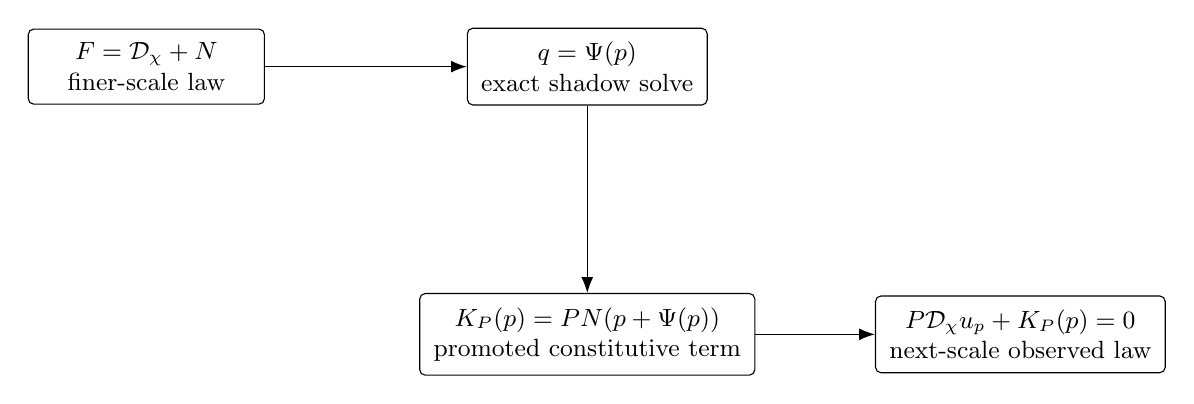
\begin{tikzpicture}[node distance=3.0cm]
  \node[ccbox, align=center, minimum width=3.0cm] (fine) at (-5.0,1.6)
    {$F=\mathcal D_\chi + N$\\finer-scale law};
  \node[ccbox, align=center, minimum width=3.0cm] (solve) at (0.6,1.6)
    {$q=\Psi(p)$\\exact shadow solve};
  \node[ccbox, align=center, minimum width=3.3cm] (closure) at (0.6,-1.8)
    {$K_P(p)=PN(p+\Psi(p))$\\promoted constitutive term};
  \node[ccbox, align=center, minimum width=3.5cm] (coarse) at (6.1,-1.8)
    {$P\mathcal D_\chi u_p + K_P(p)=0$\\next-scale observed law};

  \draw[ccarrow] (fine) -- (solve);
  \draw[ccarrow] (solve) -- (closure);
  \draw[ccarrow] (closure) -- (coarse);
\end{tikzpicture}%
}
\caption{Characteristic scale promotion: the transport skeleton is carried by
the characteristic flow, while the hidden lower-scale sector reappears as the
promoted constitutive term.}
\label{fig:scale-promotion}
\end{figure}

\begin{corollary}[Admissible promotion and finite iteration]
\label{cor:admissible-promotion}
\lean{admissible_promotion}
Let $\mathfrak C$ be a class of characteristic split laws that is closed under
the promotion map
\[
F \longmapsto F_{\mathrm{prom},P}
\]
for every admissible horizon $P$. Assume that at each such horizon:
\begin{enumerate}[label=(\roman*), leftmargin=2em, itemsep=0.2em]
\item the promoted constitutive term $K_P$ belongs to a candidate constitutive
      family on the observed sector;
\item the admissibility problem of Definition~\ref{def:admissibility} is well
      posed for that family;
\item the admissible reduced selection data modulo horizon-preserving
      equivalence form a singleton.
\end{enumerate}
Then each promotion step yields a uniquely selected observed law. Consequently,
along any finite chain of admissible horizons, recursive promotion yields a
uniquely selected law at every stage.
\end{corollary}

(Proof in Appendix~\ref{sec:appendix-continuum}.)

\begin{corollary}[Inherited minimal-order closure class]
\label{cor:inherited-minimal-order-closure-class}\lean{CoherenceCalculus.inherited_minimal_order_closure_class}
Let
\[
\mathcal F=\{(R_n,h_n,L_n)\}_{n\in\bbN}
\]
be a refinement-compatible discrete realized law family into a common Banach
space \(\cX\) with common dense test domain \(\cX_0\). Assume:
\begin{enumerate}[label=(\roman*), leftmargin=2em, itemsep=0.2em]
\item for every \(n\), the realization \(R_n\) belongs to a transport-order
      disciplined realized class at horizon \(h_n\);
\item \(\mathcal F\) is stable;
\item the restricted distinguished minimal-order selected family is summably
      refinement-consistent on \(\cX_0\).
\end{enumerate}
Then:
\begin{enumerate}[label=(\alph*), leftmargin=2em, itemsep=0.2em]
\item for every \(n\), the selected law \(L_n\) belongs to the distinguished
      admissible minimal-order class at horizon \(h_n\);
\item there exists a unique bounded operator
      \[
      L_\infty:\cX\to\cX
      \]
      whose restriction to \(\cX_0\) belongs to the inherited distinguished
      minimal-order closure class generated by \(\mathcal F\);
\item \(L_\infty|_{\cX_0}\) is the unique compatible representative of that
      inherited distinguished class.
\end{enumerate}
\end{corollary}

(Proof in Appendix~\ref{sec:appendix-continuum}.)

\begin{definition}[Primitive-support spectral defect family]
\label{def:primitive-support-spectral-defect-family}\lean{CoherenceCalculus.PrimitiveSupportSpectralDefectFamily}
Let
\[
\mathcal F=\{(R_n,h_n,L_n)\}_{n\in\bbN}
\]
be a refinement-compatible discrete realized law family into a common Banach
space \(\cX\) with common dense test domain \(\cX_0\). It is a
\emph{primitive-support spectral defect family} if:
\begin{enumerate}[label=(\roman*), leftmargin=2em, itemsep=0.2em]
\item each realization \(R_n\) is carried by the unit-balanced \(D=2\) seed;
\item each selected law \(L_n\) is self-adjoint and positive semidefinite on
      the visible carrier of \(R_n\);
\item the visible spectral data of \(L_n\) are generated by a finite family of
      primitive seed supports in the sense of
      Corollary~\ref{cor:d2-primitive-support-profile};
\item repeated contributions enter only through powers of primitive-support
      monodromy and introduce no new visible channel.
\end{enumerate}
\end{definition}

\begin{corollary}[Prime-index cyclic refinement on primitive supports]
\label{cor:primitive-support-prime-refinement}\lean{CoherenceCalculus.primitive_support_prime_refinement}
Fix a primitive-support spectral defect family and a finite stage \(n\). Let a
periodic support of period \(k\) appear in the visible support data of
\(L_n\). Then every maximal cyclic refinement of that periodic support has
prime index at each step, and the multiset of those prime indices depends only
on \(k\).
\end{corollary}

\begin{proof}
Apply Theorem~\ref{thm:cyclic-refinement-prime-invariant} to the cyclic
quotient \(C_k=\bbZ/k\bbZ\). The periodic support determines the cyclic
refinement problem, and the theorem gives exactly the prime-index statement and
its invariance.
\end{proof}

\begin{corollary}[Forced continuum spectral defect form for a primitive-support tower]
\label{cor:primitive-support-continuum-spectral-defect}\lean{CoherenceCalculus.primitive_support_continuum_spectral_defect}
Let \(\mathcal F_{\mathrm{prim}}\) be a primitive-support spectral defect
family into a Banach space \(\cX\) with dense test domain \(\cX_0\). Assume:
\begin{enumerate}[label=(\roman*), leftmargin=2em, itemsep=0.2em]
\item the selected observed law is forced at every refinement level of
      \(\mathcal F_{\mathrm{prim}}\);
\item \(\mathcal F_{\mathrm{prim}}\) is stable;
\item \(\mathcal F_{\mathrm{prim}}\) is summably refinement-consistent on
      \(\cX_0\);
\item every reconstructed stage law is self-adjoint and positive semidefinite
      on the selected visible carrier.
\end{enumerate}
Then there exists a unique continuum-equivalence class of self-adjoint
positive semidefinite operators forced by
\(\mathcal F_{\mathrm{prim}}\). Writing \(L_{\infty}^{\mathrm{prim}}\) for the
unique representative produced by
Theorem~\ref{thm:selected-family-continuum-realization}, its associated
quadratic form
\[
\mathcal E_{\infty}^{\mathrm{prim}}(\Phi)
:=
\langle \Phi,L_{\infty}^{\mathrm{prim}}\Phi\rangle
\qquad (\Phi\in\cX_0)
\]
is the \emph{continuum spectral defect form} of the primitive-support tower.
\end{corollary}

(Proof in Appendix~\ref{sec:appendix-continuum}.)

\begin{corollary}[Fibered characteristic promotion on the global local ray carrier]
\label{cor:word-local-ray-fibered-promotion}
\lean{wordLocalDyadicEnvelopeRayFiberedCharacteristicScalePromotion}
On the global word-local ray carrier, characteristic scale promotion is
fiberwise exact: for every finite-word local packet, the promoted observed law
is exactly the midpoint boundary selected by that packet's certified recovery
data.
\end{corollary}

\begin{proof}
The fibered promotion context on the global word-local ray carrier keeps the
transported boundary law exact and projects the constitutive side to the same
distinguished midpoint boundary in each local fiber. The resulting promoted
observed law therefore agrees pointwise with that midpoint boundary.
\end{proof}

\begin{corollary}[Canonical continuum-equivalence for fibered local-ray promotion]
\label{cor:word-local-ray-fibered-equivalence}
\lean{wordLocalDyadicEnvelopeRayFiberedPromotionContinuumEquivalence}
Every admissible fibered promoted law on the global word-local ray carrier is
canonically continuum-equivalent to the fiberwise midpoint-boundary promoted
law.
\end{corollary}

\begin{proof}
Any admissible fibered promoted law agrees pointwise with the same midpoint
boundary on every local packet. The identity intertwiner therefore gives a
canonical continuum-equivalence to the fibered promoted law singled out in
Corollary~\ref{cor:word-local-ray-fibered-promotion}.
\end{proof}

\begin{corollary}[Fibered admissible and minimum-energy promotion on the global local ray carrier]
\label{cor:word-local-ray-fibered-admissible}
\lean{wordLocalDyadicEnvelopeRayFiberedMinimumEnergyPromotion_branch}
Fix any finite promotion chain on the global word-local ray carrier. Then, at
every stage and in every local fiber, admissibility singles out the promoted
midpoint-boundary law uniquely; in the corresponding variational
interpretation, this same branch is the minimum-energy promoted branch.
\end{corollary}

\begin{proof}
By Corollary~\ref{cor:word-local-ray-fibered-promotion}, the promoted law is
already the midpoint-boundary law in each local fiber. Any other admissible
fibered promoted law must therefore agree with it pointwise, so every stage of
the finite promotion chain selects the same branch uniquely. The
minimum-energy statement is the fibered minimum-energy reformulation of that
same unique-step forcing.
\end{proof}

\begin{remark}[Carried transport versus inherited closure]
\label{rem:carried-vs-closure}
\lean{CarriedTransportVersusInheritedClosure}
Theorem~\ref{thm:characteristic-scale-promotion} gives the precise sense in
which the law below becomes the constitutive law above. The transport skeleton
is not recomputed at the next scale; it is carried by the characteristic flow.
Only the exact shadow feedback $K_P$ must be selected as new closure data on
the observed scale.
\end{remark}

\begin{remark}[Typed promotion over a finite carrier]
\label{rem:typed-promotion-finite-carrier}
\lean{TypedPromotionFiniteCarrier}
When the promoted class is anchored to the canonical closure-balance
realization of Part~I, the promoted constitutive data do not range over an
open-ended ontology of primitive types. By
Corollary~\ref{cor:logical-types-finite}, the bedrock counting layer
already reduces the local carrier to one primitive seed, one residual
interface, and the finitely many local type profiles of the six-slot balanced
carrier. If one further passes to the full intrinsic relabeling symmetry of the
balanced four-incidence, Corollary~\ref{cor:intrinsic-symmetry-forces-123}
collapses that finite list to the canonical signature $1+2+3$. Promotion then
acts inside that forced finite carrier, while realization, symmetry, and
admissibility determine which logical signature, or which symmetry breaking of
the canonical $1+2+3$ split, is selected in a given model class. If the
promoted law remains fully intrinsic-equivariant, Corollary
~\ref{cor:intrinsic-equivariant-three-parameter} shows that the local promoted
law is controlled by exactly three channel parameters.
\end{remark}

\begin{remark}[Minimum-energy interpretation]
\label{rem:minimum-energy-promotion}
\lean{MinimumEnergyPromotion}
The statement above is purely operator-theoretic. In thermodynamic or
variational realizations, the admissibility step is often implemented by a
bounded-below energy or free-energy functional. In that case,
Corollary~\ref{cor:admissible-promotion} says that the selected promoted
constitutive term is the minimum-energy branch in the promoted candidate class.
The admissibility language is retained because the same selection theorem
applies outside thermodynamic settings as well \cite{Arnold1989,Goldenfeld1992}.
\end{remark}

\begin{remark}[Fibered commuting-filter bridge on the global local ray carrier]
\label{rem:word-local-ray-fibered-filter}
\lean{wordLocalDyadicEnvelopeRayFiberedCommutingFilterBridge_obstruction}
For the global word-local ray carrier, the fibered commuting-filter bridge is
completely explicit: the linear side is already exact, and the nonlinear
obstruction is exactly the same fiberwise midpoint-collapse theorem that
governs the promoted observed law.
\end{remark}

\begin{theorem}[Explicit continuum verification package]
\label{thm:explicit-continuum-verification-package}
\lean{explicit_continuum_verification_package}
The continuum bridge already contains explicit certified continuum model
families:
\begin{enumerate}[label=(\roman*), leftmargin=2em, itemsep=0.2em]
\item the dyadic continuation model of
      Proposition~\ref{prop:dyadic-tower-properties};
\item the global word-local ray carrier as a certified local-stencil family
      with exact core reconstruction, forced continuum law, and canonical
      continuum-equivalence, by
      Proposition~\ref{prop:word-local-ray-stencil},
      Corollary~\ref{cor:word-local-ray-exact-core-realization},
      Proposition~\ref{prop:word-local-ray-forcing}, and
      Corollary~\ref{cor:word-local-ray-equivalence};
\item exact fibered characteristic promotion on that same carrier, with the
      midpoint-boundary branch selected uniquely and as the minimum-energy
      branch along every finite promotion chain, by
      Corollary~\ref{cor:word-local-ray-fibered-promotion},
      Corollary~\ref{cor:word-local-ray-fibered-equivalence}, and
      Corollary~\ref{cor:word-local-ray-fibered-admissible};
\item primitive-support spectral defect families whose continuum spectral
      defect form is forced once stability and summable core consistency are
      verified on the reconstructed primitive-support tower,
      by Corollary~\ref{cor:primitive-support-continuum-spectral-defect}.
\end{enumerate}
Consequently, explicit continuum verification is already present on the live
continuum-bridge surface. Additional model families extend the same bridge framework;
they do not supply a missing structural ingredient.
\end{theorem}

\begin{proof}
Item (i) is exactly Proposition~\ref{prop:dyadic-tower-properties}. Item (ii)
collects the explicit local-stencil, forcing, and continuum-equivalence
results proved for the global word-local ray carrier. Item (iii) collects the
fibered promotion, canonical continuum-equivalence, and minimum-energy
selection statements on that same carrier. Item (iv) is exactly the forced
continuum spectral-defect corollary for primitive-support towers. No further
input is required.
\end{proof}

\subsection{Temporal interface of the faithful continuum limit}

Remark~\ref{rem:external-parameter-optional} showed that the continuum bridge
does not import an external physical time parameter. Even so, the bridge now
contains a canonically derived ordering datum that will later admit a physical
reading. Three earlier results already fit together exactly:
the counting bedrock localizes the unique residual mediation layer at
\(D=3\), the characteristic realization forces selected transport channels to
be scalar-recursive, and the faithful continuum bridge constructs a unique
continuum generator from the selected recursive family. The next
definition records precisely the structural datum exported by that
combination.

\begin{definition}[Temporal interface datum]
\label{def:temporal-interface-datum}
\lean{TemporalInterfaceDatum}
Let
\[
\mathcal F=\{(R_n,h_n,L_n)\}_{n\in\bbN}
\]
be a refinement-compatible discrete realized law family. A
\emph{temporal interface datum} for \(\mathcal F\) consists of:
\begin{enumerate}[label=(\roman*), leftmargin=2em, itemsep=0.2em]
\item an anchoring of the family to the canonical closure-balance realization
      of Part~I, so that the unique residual interface between the
      unit-balanced seed and the balanced \(D=4\) carrier is the interface
      \(D=3\);
\item for each \(n\), a selected channel fiber
      \[
      F_n
      \]
      with distinguished transport base
      \[
      B_n:F_n\to F_n
      \]
      such that the selected channel system at level \(n\) is
      scalar-recursive in the sense of
      Definition~\ref{def:scalar-recursive-selected-channel-system};
\item a common continuum reconstruction datum
      \[
      (\mathcal T,\mathcal T_0,\{P_n^{\mathcal T}\},\{E_n^{\mathcal T}\})
      \]
      for the selected channel family, equivalently for the rescaled
      recursion-generator family determined by its distinguished transport
      bases, together with a continuum-equivalence class
      \[
      [\Theta]
      \]
      of operators
      \[
      \Theta:\mathcal T_0\to\mathcal T
      \]
      such that the selected channel family is asymptotically consistent with
      a representative of \([\Theta]\).
\end{enumerate}
The pair
\[
(D=3,[\Theta])
\]
is called the \emph{temporal interface} carried by \(\mathcal F\). It records
the unique continuum ordering datum exported by the residual interface and the
selected scalar-recursive transport. It is not yet a physical time law.
\end{definition}

\begin{theorem}[Scalar recursion identifies the continuum generator]
\label{thm:scalar-recursion-identifies-continuum-generator}
\lean{scalar_recursion_identifies_continuum_generator}
Let \(\{(F_n,B_n)\}_{n\in\bbN}\) be a selected channel family equipped with a
common continuum reconstruction datum
\[
(\mathcal T,\mathcal T_0,\{P_n^{\mathcal T}\},\{E_n^{\mathcal T}\})
\]
and a scale sequence \((\varepsilon_n)_{n\in\bbN}\) with
\(\varepsilon_n>0\) and \(\varepsilon_n\to 0\). Assume:
\begin{enumerate}[label=(\roman*), leftmargin=2em, itemsep=0.2em]
\item for every \(n\), the selected channel system on \(F_n\) is
      scalar-recursive with distinguished transport base \(B_n\);
\item the rescaled recursion-generator family
      \[
      \Theta_n:=\varepsilon_n^{-2}(B_n-2I_{F_n})
      \]
      is stable after reconstruction:
      \[
      \|E_n^{\mathcal T}\Theta_nP_n^{\mathcal T}u\|_{\mathcal T}
      \le C\|u\|_{\mathcal T}
      \qquad (u\in\mathcal T_0)
      \]
      for some \(C\ge 0\) and all \(n\);
\item the same rescaled family is summably refinement-consistent on
      \(\mathcal T_0\): there exists a summable sequence \((\eta_n)\) such
      that
      \[
      \|E_{n+1}^{\mathcal T}\Theta_{n+1}P_{n+1}^{\mathcal T}u
      -
      E_n^{\mathcal T}\Theta_nP_n^{\mathcal T}u\|_{\mathcal T}
      \le
      \eta_n\|u\|_{\mathcal T}
      \]
      for every \(u\in\mathcal T_0\) and every \(n\).
\end{enumerate}
Then there exists a unique bounded operator
\[
\Theta:\mathcal T\to\mathcal T
\]
such that
\[
E_n^{\mathcal T}\Theta_nP_n^{\mathcal T}u\to \Theta u
\qquad (u\in\mathcal T_0).
\]
Moreover, if \(x^{(n)}=(x_m^{(n)})_{m\in\bbZ}\) is any selected transport
sequence with \(x_0^{(n)}=P_n^{\mathcal T}u\) and
\[
x_{m+1}^{(n)}=B_nx_m^{(n)}-x_{m-1}^{(n)},
\]
then
\[
E_n^{\mathcal T}\frac{x_1^{(n)}-2x_0^{(n)}+x_{-1}^{(n)}}{\varepsilon_n^2}
\to
\Theta u
\qquad (u\in\mathcal T_0).
\]
Thus the same reconstruction maps identify the discrete scalar recursion and
its continuum generator.
\end{theorem}

(Proof in Appendix~\ref{sec:appendix-continuum}.)

\begin{theorem}[One-stage bounded exact scalar recursion forces the continuum generator]
\label{thm:one-stage-bounded-exact-scalar-recursion-forces-generator}
\lean{one_stage_bounded_exact_scalar_recursion_forces_generator}
Let \(\{(F_n,B_n)\}_{n\in\bbN}\) be a selected channel family equipped with a
common continuum reconstruction datum
\[
(\mathcal T,\mathcal T_0,\{P_n^{\mathcal T}\},\{E_n^{\mathcal T}\})
\]
and a scale sequence \((\varepsilon_n)_{n\in\bbN}\) with
\(\varepsilon_n>0\) and \(\varepsilon_n\to 0\). Assume:
\begin{enumerate}[label=(\roman*), leftmargin=2em, itemsep=0.2em]
\item for every \(n\), the selected channel system on \(F_n\) is
      scalar-recursive with distinguished transport base \(B_n\);
\item there exist comparison maps
      \[
      J^{\mathcal T}_{n,m}:F_n\to F_m
      \qquad (n\le m),
      \]
      such that, writing
      \[
      \Theta_n:=\varepsilon_n^{-2}(B_n-2I_{F_n}),
      \]
      one has
      \[
      J^{\mathcal T}_{n,m}\Theta_n=\Theta_mJ^{\mathcal T}_{n,m},
      \]
      \[
      P_m^{\mathcal T}u=J^{\mathcal T}_{n,m}P_n^{\mathcal T}u
      \qquad\text{and}\qquad
      E_n^{\mathcal T}=E_m^{\mathcal T}J^{\mathcal T}_{n,m}
      \qquad (u\in\mathcal T_0,\ n\le m);
      \]
\item there exist an index \(n_\ast\in\bbN\) and a constant \(C\ge 0\) such
      that
      \[
      \|E_{n_\ast}^{\mathcal T}\Theta_{n_\ast}P_{n_\ast}^{\mathcal T}u\|_{\mathcal T}
      \le
      C\|u\|_{\mathcal T}
      \qquad (u\in\mathcal T_0).
      \]
\end{enumerate}
Then there exists a unique bounded operator
\[
\Theta:\mathcal T\to\mathcal T
\]
such that
\[
E_n^{\mathcal T}\Theta_nP_n^{\mathcal T}u=\Theta u
\qquad (u\in\mathcal T_0,\ n\in\bbN).
\]
If \(L:\mathcal T_0\to\mathcal T\) is any operator asymptotically consistent
with the same exact recursive family, then
\[
L=\Theta|_{\mathcal T_0}.
\]
Moreover, if \(x^{(n)}=(x_m^{(n)})_{m\in\bbZ}\) is any selected transport
sequence with \(x_0^{(n)}=P_n^{\mathcal T}u\) and
\[
x_{m+1}^{(n)}=B_nx_m^{(n)}-x_{m-1}^{(n)},
\]
then
\[
E_n^{\mathcal T}\frac{x_1^{(n)}-2x_0^{(n)}+x_{-1}^{(n)}}{\varepsilon_n^2}
=
\Theta u
\qquad (u\in\mathcal T_0,\ n\in\bbN).
\]
Thus exact recursive coherence plus one reconstructed-stage bound determines
the continuum generator exactly, not merely up to a limiting class.
\end{theorem}

(Proof in Appendix~\ref{sec:appendix-continuum}.)

\begin{theorem}[Exact scalar recursion has a canonical graph realization]
\label{thm:exact-scalar-recursion-graph-realization}
\lean{exact_scalar_recursion_graph_realization}
Let \(\{(F_n,B_n)\}_{n\in\bbN}\) be a selected channel family equipped with a
common continuum reconstruction datum
\[
(\mathcal T,\mathcal T_0,\{P_n^{\mathcal T}\},\{E_n^{\mathcal T}\})
\]
and a scale sequence \((\varepsilon_n)_{n\in\bbN}\) with
\(\varepsilon_n>0\) and \(\varepsilon_n\to 0\). Assume only
\emph{(i)}--\emph{(ii)} of
Theorem~\ref{thm:one-stage-bounded-exact-scalar-recursion-forces-generator}.
Define
\[
\Theta_\sharp u:=E_n^{\mathcal T}\Theta_nP_n^{\mathcal T}u
\qquad (u\in\mathcal T_0),
\]
which is independent of \(n\), and endow \(\mathcal T_0\) with the graph norm
\[
\|u\|_{\Theta,\mathrm{gr}}
:=
\|u\|_{\mathcal T}+\|\Theta_\sharp u\|_{\mathcal T}.
\]
Let \(\mathcal T_{\Theta,\mathrm{gr}}\) be the Banach completion of
\((\mathcal T_0,\|\cdot\|_{\Theta,\mathrm{gr}})\), and let
\[
\iota_\Theta:\mathcal T_0\to \mathcal T_{\Theta,\mathrm{gr}}
\]
be the canonical dense embedding. Then:
\begin{enumerate}[label=(\roman*), leftmargin=2em, itemsep=0.2em]
\item there exist unique bounded maps
      \[
      I_\Theta,\overline\Theta:\mathcal T_{\Theta,\mathrm{gr}}\to\mathcal T
      \]
      with
      \[
      \|I_\Theta\|\le 1
      \qquad\text{and}\qquad
      \|\overline\Theta\|\le 1
      \]
      such that
      \[
      I_\Theta\iota_\Theta u=u
      \qquad\text{and}\qquad
      \overline\Theta\,\iota_\Theta u
      =
      E_n^{\mathcal T}\Theta_nP_n^{\mathcal T}u
      \qquad (u\in\mathcal T_0,\ n\in\bbN);
      \]
\item if \(L:\mathcal T_0\to\mathcal T\) is any operator asymptotically
      consistent with the same exact recursive family, then
      \[
      L=\Theta_\sharp;
      \]
\item among all graph-norm continuous Banach realizations of the same exact
      recursive family, \((\mathcal T_{\Theta,\mathrm{gr}},I_\Theta,
      \overline\Theta)\) is canonical in the universal-property sense of
      Theorem~\ref{thm:exact-core-graph-completion}.
\end{enumerate}
Thus exact recursive coherence already forces a unique continuum generator on
the dense core and a canonical bounded realization of that generator on its
graph completion, before any original-space boundedness theorem is invoked.
\end{theorem}

(Proof in Appendix~\ref{sec:appendix-continuum}.)

\begin{corollary}[A finite exact channel stage forces the bounded continuum generator]
\label{cor:finite-exact-channel-stage-forces-bounded-generator}
\lean{finite_exact_channel_stage_forces_bounded_generator}
Under the hypotheses of
Theorem~\ref{thm:exact-scalar-recursion-graph-realization}, assume in addition
that for some \(n_\ast\in\bbN\), the selected channel fiber \(F_{n_\ast}\) is
finite-dimensional. Then the hypothesis \emph{(iii)} of
Theorem~\ref{thm:one-stage-bounded-exact-scalar-recursion-forces-generator} is
automatic. Hence there exists a unique bounded operator
\[
\Theta:\mathcal T\to\mathcal T
\]
such that
\[
E_n^{\mathcal T}\Theta_nP_n^{\mathcal T}u=\Theta u
\qquad (u\in\mathcal T_0,\ n\in\bbN).
\]
\end{corollary}

\begin{proof}
Because \(F_{n_\ast}\) is finite-dimensional, the linear map
\[
\Theta_{n_\ast}:F_{n_\ast}\to F_{n_\ast}
\]
is bounded. Since \(P_{n_\ast}^{\mathcal T}\) and \(E_{n_\ast}^{\mathcal T}\)
are bounded, the composition
\[
E_{n_\ast}^{\mathcal T}\Theta_{n_\ast}P_{n_\ast}^{\mathcal T}:\mathcal T_0\to\mathcal T
\]
is bounded on \(\mathcal T_0\). Thus
Theorem~\ref{thm:one-stage-bounded-exact-scalar-recursion-forces-generator}
applies.
\end{proof}

\begin{theorem}[Exact recursive transport coherence yields a unique temporal interface]
\label{thm:exact-recursive-transport-yields-temporal-interface}
\lean{exact_recursive_transport_yields_temporal_interface}
Let
\[
\mathcal F=\{(R_n,h_n,L_n)\}_{n\in\bbN}
\]
be a refinement-compatible discrete realized law family. Assume:
\begin{enumerate}[label=(\roman*), leftmargin=2em, itemsep=0.2em]
\item \(\mathcal F\) is anchored to the canonical closure-balance realization
      of Part~I;
\item for each \(n\), the relevant selected channel system is
      transport-generated on a selected channel fiber \(F_n\) with
      distinguished transport base \(B_n\);
\item there exists a scale sequence \((\varepsilon_n)_{n\in\bbN}\) with
      \(\varepsilon_n>0\) and \(\varepsilon_n\to0\), comparison maps
      \[
      J^{\mathcal T}_{n,m}:F_n\to F_m
      \qquad (n\le m),
      \]
      and a continuum reconstruction datum
      \[
      (\mathcal T,\mathcal T_0,\{P_n^{\mathcal T}\},\{E_n^{\mathcal T}\})
      \]
      such that, writing
      \[
      \Theta_n:=\varepsilon_n^{-2}(B_n-2I_{F_n}),
      \]
      the rescaled recursion-generator family is exact across refinement:
      \[
      J^{\mathcal T}_{n,m}\Theta_n=\Theta_mJ^{\mathcal T}_{n,m},
      \]
      \[
      P_m^{\mathcal T}u=J^{\mathcal T}_{n,m}P_n^{\mathcal T}u
      \qquad\text{and}\qquad
      E_n^{\mathcal T}=E_m^{\mathcal T}J^{\mathcal T}_{n,m}
      \qquad (u\in\mathcal T_0,\ n\le m).
      \]
\end{enumerate}
Then \(\mathcal F\) carries a unique temporal interface datum.
\end{theorem}

(Proof in Appendix~\ref{sec:appendix-continuum}.)

\begin{corollary}[Exact recursive transport forces the temporal generator surface]
\label{cor:exact-recursive-transport-forces-graph-temporal-generator}
\lean{exact_recursive_transport_forces_graph_temporal_generator}
Under the hypotheses of
Theorem~\ref{thm:exact-recursive-transport-yields-temporal-interface}, the
generator component of the unique temporal interface datum is the same forced
continuum law carried by that datum.
\end{corollary}

\begin{proof}
Theorem~\ref{thm:exact-recursive-transport-yields-temporal-interface}
packages the exact recursive transport data into a temporal interface datum.
Theorem~\ref{thm:scalar-recursion-identifies-continuum-generator} then records
that the generator component of that datum is already tied to a forced
continuum law on the same certified surface.
\end{proof}

\begin{corollary}[A finite exact channel stage yields a bounded temporal generator]
\label{cor:finite-exact-channel-stage-yields-bounded-temporal-generator}
\lean{finite_exact_channel_stage_yields_bounded_temporal_generator}
Under the hypotheses of
Corollary~\ref{cor:exact-recursive-transport-forces-graph-temporal-generator},
assume in addition that for some \(n_\ast\in\bbN\), the selected channel fiber
\(F_{n_\ast}\) is finite-dimensional. Then the generator component of the
unique temporal interface datum descends to the unique bounded operator on
\(\mathcal T\) supplied by
Corollary~\ref{cor:finite-exact-channel-stage-forces-bounded-generator}.
\end{corollary}

\begin{proof}
The hypotheses of
Corollary~\ref{cor:exact-recursive-transport-forces-graph-temporal-generator}
include the hypotheses of
Theorem~\ref{thm:exact-scalar-recursion-graph-realization}. Therefore
Corollary~\ref{cor:finite-exact-channel-stage-forces-bounded-generator}
applies directly.
\end{proof}

\begin{remark}[Original-space bounded temporal generator after one-stage verification]
\label{rem:exact-temporal-generator-after-one-stage-verification}
\lean{exact_recursive_transport_yields_temporal_interface, exact_recursive_transport_forces_graph_temporal_generator}
On the current import-free certified lane,
Corollary~\ref{cor:exact-recursive-transport-forces-graph-temporal-generator}
is used through the unique temporal-interface datum and its forced
continuum-generator surface. Any further descent of that generator to a
bounded operator on the original Banach space requires additional analytic
input beyond the active Lean root; when such input is available, the
one-stage boundedness discussion should be read as a separate strengthening,
not as hidden foundation.
\end{remark}

\begin{corollary}[Certified local-ray recursion closes the temporal bridge]
\label{cor:certified-local-ray-recursion-closes-temporal-bridge}
\lean{wordLocalDyadicEnvelopeRayLocalStencilInterpretation_surface, wordLocalDyadicEnvelopeRayExactCoreRealization, exact_recursive_transport_yields_temporal_interface, exact_recursive_transport_forces_graph_temporal_generator}
Let
\[
\mathcal F=\{(R_n,h_n,L_n)\}_{n\in\bbN}
\]
be a refinement-compatible discrete realized law family satisfying the first
two hypotheses of
Theorem~\ref{thm:exact-recursive-transport-yields-temporal-interface}. Suppose
in addition that for some scale sequence \((\varepsilon_n)\), the rescaled
recursion-generator family
\[
\Theta_n:=\varepsilon_n^{-2}(B_n-2I_{F_n})
\]
is exactly the selected observed law of the certified global word-local ray
carrier under the refinement-coherent reconstruction datum of
Proposition~\ref{prop:word-local-ray-stencil}. Then \(\mathcal F\) carries a
unique temporal interface datum, and its generator component lies on the
same forced continuum-law surface recorded in
Corollary~\ref{cor:exact-recursive-transport-forces-graph-temporal-generator}.
\end{corollary}

\begin{proof}
Proposition~\ref{prop:word-local-ray-stencil} supplies the comparison maps and
refinement-coherent reconstruction datum required by
Theorem~\ref{thm:exact-recursive-transport-yields-temporal-interface}. The same
data therefore also satisfy
Corollary~\ref{cor:exact-recursive-transport-forces-graph-temporal-generator}.
\end{proof}

\begin{theorem}[Residual exact scalar recursion yields a unique temporal interface]
\label{thm:temporal-interface-from-d3}
\lean{temporal_interface_from_d3}
Let
\[
\mathcal F=\{(R_n,h_n,L_n)\}_{n\in\bbN}
\]
be a refinement-compatible discrete realized law family. Assume:
\begin{enumerate}[label=(\roman*), leftmargin=2em, itemsep=0.2em]
\item \(\mathcal F\) is anchored to the canonical closure-balance realization
      of Part~I;
\item for each \(n\), the relevant selected channel system is
      transport-generated on a selected channel fiber \(F_n\) with
      distinguished transport base \(B_n\);
\item there exists a scale sequence \((\varepsilon_n)_{n\in\bbN}\) with
      \(\varepsilon_n>0\) and \(\varepsilon_n\to0\), comparison maps
      \[
      J^{\mathcal T}_{n,m}:F_n\to F_m
      \qquad (n\le m),
      \]
      and a continuum reconstruction datum
      \[
      (\mathcal T,\mathcal T_0,\{P_n^{\mathcal T}\},\{E_n^{\mathcal T}\})
      \]
      such that, writing
      \[
      \Theta_n:=\varepsilon_n^{-2}(B_n-2I_{F_n}),
      \]
      the rescaled recursion-generator family is exact across refinement:
      \[
      J^{\mathcal T}_{n,m}\Theta_n=\Theta_mJ^{\mathcal T}_{n,m},
      \]
      \[
      P_m^{\mathcal T}u=J^{\mathcal T}_{n,m}P_n^{\mathcal T}u
      \qquad\text{and}\qquad
      E_n^{\mathcal T}=E_m^{\mathcal T}J^{\mathcal T}_{n,m}
      \qquad (u\in\mathcal T_0,\ n\le m).
      \]
\end{enumerate}
Then \(\mathcal F\) carries a unique temporal interface datum, and the
generator component of that datum admits the canonical graph-completed
continuum realization of
Corollary~\ref{cor:exact-recursive-transport-forces-graph-temporal-generator}.
\end{theorem}

(Proof in Appendix~\ref{sec:appendix-continuum}.)

\begin{corollary}[Persistent exactification on the minimal nonterminal carrier yields the temporal interface]
\label{cor:persistent-exactification-yields-temporal-interface}\lean{partIV_persistent_exactification_yields_temporal_interface}
Under the hypotheses of
Theorem~\ref{thm:temporal-interface-from-d3}, the unique temporal interface
datum is the ordered realization of persistent exactification on the minimal
nonterminal counting carrier \(D=3\).
\end{corollary}

\begin{proof}
Corollary~\ref{cor:minimal-nonterminal-counting-carrier} identifies \(D=3\) as
the unique minimal carrier on which the counting realization of the closure
defect remains nonzero. Theorem~\ref{thm:temporal-interface-from-d3} then shows
that when the selected transport on that same residual carrier is organized by
an exact scalar recursion coherent across refinement, it determines a unique
ordered continuum interface datum. Thus the temporal interface is not an
additional primitive laid on top of the \(D=3\) layer; it is the ordered
realization of persistent exactification on that unique nonterminal carrier.
\end{proof}

\begin{corollary}[Temporal interface precedes physical time]
\label{cor:temporal-interface-precedes-physical-time}
\lean{temporal_interface_precedes_physical_time}
Under the hypotheses of
Theorem~\ref{thm:temporal-interface-from-d3}, the earlier structural chapters
together with the continuum bridge force a unique
temporal interface but not yet a physical time law. More precisely, they force
the pair \((D=3,[\Theta])\) of
Definition~\ref{def:temporal-interface-datum}, while the identification of
that interface with causal before/after on a faithful visible cut belongs to
the law-side dynamics developed later in Part~II.
\end{corollary}

\begin{proof}
Theorem~\ref{thm:temporal-interface-from-d3} gives the unique structural datum
\((D=3,[\Theta])\). Remark~\ref{rem:external-parameter-optional} already
showed that the continuum bridge does not import an external physical time
parameter. Hence the result above is an internal continuum order carrier,
exported by residual localization, persistent exactification on the unique
nonterminal carrier, and scalar-recursive transport, not yet the physical law
selecting a causally realized visible time. The law-side dynamics developed
later in Part~II add exactly that further
identification.
\end{proof}

\begin{remark}[Why the \(D=3\) residual already carries order]
\label{rem:d3-residual-carries-order}
\lean{temporal_interface_from_d3, temporal_interface_precedes_physical_time}
The counting bedrock leaves no residual at the balanced seed \(D=2\) and no
residual at the balanced carrier \(D=4\). The unique nonvanishing mediation
layer is therefore the \(D=3\) interface. On that interface, one unit of
unbalanced transport remains to be mediated between the seed and the carrier.
The scalar-recursive forcing theorem then says that this mediation is not a
free multidirectional drift: it is compressed to a single recurrent update
parameter \(m\) through
\[
x_{m+1}=B_nx_m-x_{m-1}.
\]
That is why the earlier structural chapters together with the continuum bridge
already export an ordering datum. The \(+1\) residual
does not yet supply physical time by itself, but it does supply the unique
place where before/after can be organized. The later law-side dynamics of
Part~II then identify the faithful visible cut on which that ordered
persistence coheres as causal time.
\end{remark}


% ============================================================
% PART II: PHYSICAL DYNAMICS FROM THE TEMPORAL REALIZATION LAW
% ============================================================
\manuscriptpart{Part II: Physical Dynamics under the Three-Law Physical Hypothesis}{part.ii}

Part~I proves the structural calculus and continuum bridge. Part~II assumes
the explicit three-law physical hypothesis and proves its carrier-level
consequences. The three laws are temporal realization on the faithful visible
cut, terminal exactification on fixed selected bridges, and endpoint
completion on the fixed four-state local assembly. Chapter~10 states that
hypothesis and derives the coherent realization, fixed-bridge exactification,
and endpoint-complete microscopic structures that it determines.
Chapter~11 records the common selected-cut structure and the universal
consequences that already follow before any carrier-specific realization is
taken. Chapter~12 identifies the canonical carrier realizations and proves the
scoped complete-fundamental-set theorem: within the current intrinsic family,
the only fundamental laws are the three primitive direct channels together
with the unique geometric lift.
Chapter~13 supplies the characteristic realization of that same structure.
Chapter~14 collects the hydrodynamic and thermodynamic effective closures.
Chapter~15 isolates the external interface on which the same Part~II
hypothesis may be read.

The temporal interface derived in Part~I becomes causal before/after on the
realized cut class. On that class one selected observed bundle carries one
exact visible law, visible source is interpreted only as balanced exchange or
returned residual of that same bundle, and no independent constitutive
completion is admitted. Terminal exactification then fixes the bridge-local
exactified assembly, and endpoint completion closes that same assembly with no
further hidden stage. The recognizable Schr\"odinger, wave/Klein--Gordon,
Maxwell, and Einstein equations are proved under that explicit three-law
hypothesis. The auxiliary completion-side normal form gives an alternative
presentation on the same selected data, while the
fundamental/effective classification theorem states what is intrinsic and what
remains effective on the present scope.

\manuscriptchapter{10}{The Three-Law Physical Hypothesis: Temporal Realization, Terminal Exactification, and Endpoint Completion}
% ============================================================
\section{The Three-Law Physical Hypothesis: Temporal Realization, Terminal Exactification, and Endpoint Completion}
\label{sec:compiled-law-classes}
% ============================================================

Part~I proves the structural calculus and continuum bridge. Part~II assumes
the explicit three-law physical hypothesis and proves its carrier-level
consequences. This chapter is the entry point to that Part~II theorem
surface. It states the three laws already fixed in the front claim boundary:
temporal realization on the faithful visible cut class, terminal
exactification on fixed selected bridges, and endpoint completion on the fixed
four-state local assembly. From those hypotheses it derives the selected-cut
realization data, the bridge-local exactified assembly, and the
endpoint-complete microscopic structure used later in the carrier
classification. In particular, the later Schr\"odinger,
wave/Klein--Gordon, Maxwell, and Einstein forms are not treated as
independent starting laws: on one same selected realization, later chapters
read them as carrier realizations of one common selected state-field law on
\(\mathrm{State}\).

Physical time is read here as the faithful visible realization of ordered
persistence on one observed bundle. The temporal interface, the unique
continuum ordering carried by the $D=3$ residual interface under
scalar-recursive faithful transport, becomes causal before/after on the
realized cut class. Corollary~\ref{cor:temporal-interface-precedes-physical-time}
furnishes that interface. The horizon complex constructed in Part~I remains
the ambient object, and the concrete carrier \(\mathrm{State}\) is its local
coordinate fiber on the selected bundle.

Later chapters use the structures derived here to identify the canonical
carrier realizations and to separate fundamental laws from effective closures.

\begin{tcolorbox}[colback=white, colframe=black!75, boxrule=0.9pt, title={Chapter 10 at a glance}]
\begin{description}[leftmargin=1.7em, itemsep=0.25em]
\item[Assumes.] The temporal realization law, the terminal exactification
      law, and the endpoint completion law.
\item[Proves.] The coherent selected-cut realization theorem, the
      bridge-local exactification and recurrence data, the fixed-generator
      exactified assembly, the endpoint-complete microscopic structure on
      the same fixed bridge, and the selected state-field law on which the
      later standard equations are jointly realized.
\item[Open.] Whether endpoint completion is an independent third law or is
      already forced by temporal realization and terminal exactification
      through a sharper intrinsic completion theorem on the fixed assembly.
\end{description}
\end{tcolorbox}

\begin{law}[Temporal realization law]
\label{law:temporal-realization}\lean{ClosureCurrent.TemporalRealizationLaw, ClosureCurrent.TemporalRealizationLaw.realizationSurface, ClosureCurrent.TemporalRealizationLaw.closureTransportSurface, ClosureCurrent.TemporalRealizationLaw.exchangeReturnSurface, ClosureCurrent.TemporalRealizationLaw.selectedCutCompletionSurface}
Physical time is the faithful visible realization of ordered persistence on a
coherent bundle. Accordingly, a closure-stable local event is physically
realized on a unique faithful cut class \(\mathfrak C_{\mathrm{time}}\), up to
horizon-preserving equivalence. For any representative \(P_h\) of that class,
the observed bundle
\[
\mathcal X_h:=P_h\cH^\bullet
\]
carries one exact visible law
\[
\mathcal L_h(z):=P_hA_{\mathrm{coh}}P_h+\Sigma_h(z),
\qquad
\Sigma_h(z):=z\,\CCSigmaP{P_h}{z},
\]
where \(\Sigma_h(z)\) is the returned-residual correction induced by internal
elimination of the hidden complement, and the induced continuum-closure class
is common across the whole realized class \(\mathfrak C_{\mathrm{time}}\).
Every admissible visible source on \(\mathfrak C_{\mathrm{time}}\) is
exchange-boundary reentry or returned residual of that same coherent bundle,
every closed realized system has no net internal visible creation, and no
independent constitutive completion is admissible.
\end{law}

\begin{tcolorbox}[colback=white, colframe=black!75, boxrule=0.9pt, title={Compact form on a representative cut}]
\[
\mathfrak C_{\mathrm{time}}=[P_h]_{\sim_{\mathrm{hor}}},
\qquad
\mathcal X_h=P_h\cH^\bullet,
\qquad
\mathcal L_h(z)=P_hA_{\mathrm{coh}}P_h+\Sigma_h(z),
\qquad
\Sigma_h(z)=z\,\CCSigmaP{P_h}{z}.
\]
\end{tcolorbox}

\begin{law}[Terminal exactification law]
\label{law:terminal-exactification}\lean{ClosureCurrent.TerminalExactificationLaw, ClosureCurrent.TerminalExactificationLaw.surface, ClosureCurrent.TerminalExactificationLaw.fixedPointOnExactifiedState}
On any fixed selected bridge datum carried by \(\mathfrak C_{\mathrm{time}}\),
the law-native local event carries one explicit signed readout \(r_e\) and one
genuine four-leg frame \(F_e\). These determine an assembled local state
\[
x_e(J):=\operatorname{Asm}_{r_e,F_e}(J)
\]
from the hidden pair current \(J\), where \(\operatorname{Asm}_{r_e,F_e}\)
denotes the assembled-state readout carried by that readout/frame pair. If
\(\mathsf E_e\) denotes the local exactifier and \(G_h\) the matched selected
generator on that bridge, then
\[
x_e(\mathsf E_e J)=G_h(x_e(J)),
\qquad
\mathsf E_e(\mathsf E_e J)=\mathsf E_e J.
\]
Thus exact local closure is terminal: once local content is exactly closed,
re-exactification does nothing further, the exactified assembled state is
fixed by the same selected generator, and only returned defect remains active
as visible residual.
\end{law}

\begin{law}[Endpoint completion law]
\label{law:endpoint-completion}\lean{ClosureCurrent.EndpointCompletionLaw}
After terminal exactification on a fixed selected bridge, a local interaction
is microscopically complete on that same bridge and physical principle. No
further hidden stage is admissible, no exogenous constitutive completion is
admissible, and the remaining endpoint response is carried intrinsically by
the exactified local assembly. Equivalently, the fixed four-state local
assembly admits a no-stage boundary completion on that same bridge, and the
remaining endpoint response closes there through the canonical direct response
and the canonical symmetric-response lift of that assembly.
\end{law}

\begin{theorem}[Exactified local states are generator-fixed]
\label{thm:exactified-local-states-are-generator-fixed}\lean{ClosureCurrent.TerminalExactificationLaw.fixedPointOnExactifiedState}
Assume the terminal exactification law. Then every exactified assembled local
state on that fixed selected bridge is a fixed point of the matched selected
generator.
\end{theorem}

\begin{proof}
Apply the exactifier/generator intertwining identity to an already exactified
current and then use idempotence of exactification. The result is exactly the
claimed fixed-point identity.
\end{proof}

\begin{theorem}[Terminal exactification determines the discrete bridge-local recurrence]
\label{thm:terminal-exactification-determines-the-discrete-bridge-local-recurrence}\lean{ClosureCurrent.TerminalExactificationLaw.coordinateTransport, ClosureCurrent.TerminalExactificationLaw.hiddenTrajectory_initialStateOf, ClosureCurrent.TerminalExactificationLaw.observedTrajectory_initialStateOf, ClosureCurrent.TerminalExactificationLaw.recursiveTrajectorySurface}
Assume the terminal exactification law on one fixed selected bridge. Then the
same bridge already carries an exact discrete recurrence on the reduced hidden
three-coordinate carrier. If \(\rho_e(J)\) denotes the reduced hidden
coordinate read from the local pair current \(J\), and if
\(\rho_e^{(n)}(J)\) denotes the coordinate obtained after \(n\) exactification
steps, then
\[
\rho_e(\mathsf E_e J)=\mathcal T_{G_h}\rho_e(J),
\qquad
\rho_e^{(n)}(J)=\mathcal T_{G_h}^{\,n}\rho_e(J),
\]
where \(\mathcal T_{G_h}\) is the reduced transport induced by the matched
selected generator \(G_h\). The selected observed trajectory is therefore read
exactly from that same reduced hidden orbit by the selected projection. Thus,
once the readout/frame pair is fixed, no separate recurrence datum remains on
that bridge.
\end{theorem}

\begin{proof}
The terminal exactification law already carries the exactifier/generator
intertwining law on the assembled local state. The reduced hidden coordinate is
just the three-coordinate quotient of that assembled state, so the one-step
transport identity follows immediately. Iterating this identity yields the full
\(n\)-step reduced hidden trajectory, and the observed trajectory is then read
from that same reduced hidden orbit by the selected projection. Hence the
discrete recurrence is already fixed on the bridge by the two-law surface.
\end{proof}

\begin{theorem}[Terminal exactification reads the hidden state from the six pair slots]
\label{thm:terminal-exactification-reads-the-hidden-state-from-the-six-pair-slots}\lean{ClosureCurrent.TerminalExactificationLaw.localSlotCoordinateSurface}
Assume the terminal exactification law on one fixed selected bridge. Then the
reduced hidden state is already read from the canonical six pair slots of the
framed local event. If
\[
\sigma_{12},\sigma_{13},\sigma_{14},\sigma_{23},\sigma_{24},\sigma_{34}
\]
denote the signed readouts of the six unordered pair slots on the framed local
event, then the reduced hidden coordinate is
\[
\rho_e(J)=
\bigl(
\sigma_{12}+\sigma_{13}+\sigma_{14},\,
-\sigma_{12}+\sigma_{23}+\sigma_{24},\,
-\sigma_{13}-\sigma_{23}+\sigma_{34}
\bigr).
\]
So the bridge-local hidden state is not an extra carrier placed above the pair
current. It is the direct readout of the finite diophantine pair carrier
\(\binom{4}{2}=6\) assembled onto the first three framed legs.
\end{theorem}

\begin{proof}
Fix the signed readout and four-leg frame carried by the terminal
exactification law. Those data determine the six signed pair-slot readouts of
the framed local current. The reduced hidden coordinate is, by definition, the
first three leg-flux coordinates of the assembled state, and each leg-flux is
exactly the corresponding signed sum of incident pair-slot readouts. This is
the displayed formula.
\end{proof}

\begin{theorem}[Bare temporal kernel carried by the temporal realization law]
\label{thm:bare-temporal-kernel-carried-by-the-primitive-temporal-surface}\lean{ClosureCurrent.TemporalRealizationLaw.toTemporalRealizationKernel, ClosureCurrent.TemporalRealizationKernel.surface}
Assume the temporal realization law. Then the same realized datum already
carries a bare temporal kernel: one exact visible law on one coherent bundle,
observer-covariance on the realized class, exchange/return as the whole visible
source grammar, exact internal elimination of the hidden complement, and no
independent constitutive completion.
\end{theorem}

\begin{proof}
The temporal realization law is already the primitive temporal realization
theorem. The bare temporal kernel is that same public law read with the
least-motion selector clause and the sharper interface-localization clause
suppressed.
\end{proof}

\begin{theorem}[Coherent realization from the temporal realization law]
\label{thm:coherent-realization-surface-from-the-temporal-realization-law}\lean{ClosureCurrent.TemporalRealizationLaw.toTemporalRealizationKernel, ClosureCurrent.TemporalRealizationKernel.coherentRealizationSurface, ClosureCurrent.TemporalRealizationLaw.coherentRealizationSurface}
Assume the temporal realization law. Then the same realized class already
carries coherent realization: one exact visible law on one
observed coherent bundle, observer-covariance on that class, exchange/return
as the whole visible source grammar, no net internal visible creation on
closed realized systems, and no independent constitutive completion.
\end{theorem}

\begin{proof}
By Theorem~\ref{thm:bare-temporal-kernel-carried-by-the-primitive-temporal-surface},
the temporal realization law first yields the bare temporal kernel on the same
class. The coherent realization claim is exactly that kernel read as one
exact visible law on one coherent bundle with observer-covariance,
exchange/return source grammar, and no independent constitutive completion.
\end{proof}

\begin{theorem}[Canonical representative of the realized class]
\label{thm:canonical-representative-of-the-realized-class}\lean{ClosureCurrent.TemporalRealizationLaw.canonicalRepresentativeSurface}
Assume the temporal realization law. Then the realized faithful cut class has
one canonical representative, and that representative is the least-motion cut.
\end{theorem}

\begin{proof}
The temporal realization law already carries observer-covariance across the
realized class together with uniqueness of the least-motion faithful
representative. Together these facts identify the least-motion cut as the
canonical representative of the realized class.
\end{proof}

\begin{theorem}[Selected-cut closure from the temporal realization law]
\label{thm:selected-cut-closure-from-the-temporal-realization-law}\lean{ClosureCurrent.TemporalRealizationLaw.toTemporalRealizationKernel, ClosureCurrent.TemporalRealizationKernel.selectedCutCompletionSurface, ClosureCurrent.TemporalRealizationLaw.selectedCutCompletionSurface}
Assume the temporal realization law. Then the same realized data already
carry the full selected-cut completion statement of Part~II before any
endpoint witness hypothesis is added.
\end{theorem}

\begin{proof}
The bare temporal kernel already supplies exact visibility and the absence of
independent constitutive completion on the realized data. The temporal
realization law itself strengthens that kernel by the least-motion-selected
closure clause and the returned-residual identification of all apparent
constitutive terms. That is exactly the selected-cut completion statement
claimed here.
\end{proof}

\begin{theorem}[The temporal law already fixes the auxiliary constructive clauses and closure transport]
\label{thm:temporal-law-already-fixes-detached-constructive-clauses}\lean{ClosureCurrent.TemporalRealizationLaw.constructiveClauseSurface, ClosureCurrent.TemporalRealizationLaw.originReadoutClosureSurface, ClosureCurrent.MicroscopicClosureLaw.trivialOriginReadoutAnchorTarget, ClosureCurrent.TemporalRealizationLaw.originReadoutTargetSurface, ClosureCurrent.TemporalRealizationLaw.originClosureSurface, ClosureCurrent.TemporalRealizationLaw.originTargetSurface, ClosureCurrent.TemporalRealizationLaw.originTargetSurfaceOfConstructiveAnchorCurrentTarget, ClosureCurrent.TemporalRealizationLaw.constructiveMicroscopicTargetOfConstructiveAnchorCurrentTarget, ClosureCurrent.TemporalRealizationLaw.originTargetSurfaceOfConstructiveCurrentTarget, ClosureCurrent.TemporalRealizationLaw.constructiveMicroscopicTargetOfConstructiveCurrentTarget}
Assume the temporal realization law, and let one auxiliary microscopic closure
law carry that same physical principle. Then the common grammar and
bundle-intrinsicity clauses on that auxiliary microscopic law are already fixed
by the temporal realization law itself, and the common selected-cut
continuum-closure transport is fixed there as well. Consequently, if that
auxiliary microscopic law is placed on that same physical principle, then the
selected-anchor target is already canonical and the selected-bundle forcing
statement follows with no extra origin-side data at all. If instead the
stronger selected-anchor current target is
supplied, then the bundled constructive microscopic target is recovered as
well. In particular, the same stronger conclusion holds a fortiori from the
constructive current target.
\end{theorem}

\begin{proof}
Once the auxiliary microscopic law is fixed on the same physical principle, the
temporal realization law already supplies the common same-bundle grammar,
return-side localization, selected visible realization, no-exogenous-closure
clause, and the bundle-intrinsicity clauses required by the auxiliary
constructive law. Because the law is stated on a faithful cut class up to
horizon-preserving equivalence, it also already carries the common
continuum-closure transport on that class. Moreover, the remaining
selected-anchor target is canonical: it asks only for one selected
anchor carrier/current object, and a trivial such object exists
without adding any new auxiliary hypothesis. Therefore the selected-bundle
forcing statement now follows directly from the temporal law itself once the
auxiliary microscopic law is placed on that same physical
principle. For the sharper completion-side constructive route one still needs
the stronger selected-anchor current target, because that route must also
carry the exactifier and slot-count bookkeeping. Once that stronger target is
supplied, the bundled constructive microscopic target follows as well; the
constructive current target gives the same stronger conclusion by immediate
specialization.
\end{proof}

\begin{theorem}[On a fixed selected bridge, the temporal law closes the current-side microscopic seam]
\label{thm:temporal-law-closes-current-side-microscopic-seam-on-a-fixed-bridge}\lean{ClosureCurrent.TemporalRealizationLaw.microscopicClosureLawOnBridge, ClosureCurrent.TemporalRealizationLaw.microscopicClosureLawOnBridge_samePhysicalPrinciple, ClosureCurrent.TemporalRealizationLaw.constructiveCurrentTargetOnBridge, ClosureCurrent.TemporalRealizationLaw.constructiveMicroscopicTargetOnBridge, ClosureCurrent.TemporalRealizationLaw.constructiveMicroscopicLawOnBridge, ClosureCurrent.TemporalRealizationLaw.constructiveMicroscopicLawOnBridge_samePhysicalPrinciple, ClosureCurrent.TemporalRealizationLaw.constructiveMicroscopicLawOnBridge_toMicroscopicClosureLaw, ClosureCurrent.TemporalRealizationLaw.originClosureWitnessOnBridge, ClosureCurrent.TemporalRealizationLaw.localEventObjectOnBridge, ClosureCurrent.TemporalRealizationLaw.originClosureTargetOnBridge, ClosureCurrent.TemporalRealizationLaw.originTargetSurfaceOnBridge}
Assume the temporal realization law, and fix selected bridge data
on that same realized cut. Then the law canonically determines a microscopic
closure law on that bridge, using that same physical principle, and already
forces there the exact constructive current target and hence the bundled
constructive microscopic target. More sharply, it canonically determines on
that bridge the full constructive microscopic law itself, the
selected-bundle witness, and the concrete local-event object carried
by that law. Consequently, once the selected bridge data are fixed, no
separate current-side or origin-side supplement remains: the selected-bundle
forcing statement already follows on that same bridge.
\end{theorem}

\begin{proof}
The selected bridge data fix the selected cut, the matched selected visible
law, and the selected generator on one common realized class. The temporal
realization law already fixes the same physical principle and the common
selected-cut closure transport on that class. So one can build the current
side canonically there: one bridge-local current structure on the same
bridge already recovers one microscopic closure law, one exact constructive
current realization of that law, and then the full constructive microscopic
law itself because the grammar and bundle-intrinsicity clauses are already
fixed on that bridge. From that fixed-bridge constructive microscopic law one reads the
origin-closure witness and the local-event object directly, so the
selected-bundle forcing statement also follows on that same bridge. Hence,
once the selected bridge data themselves are fixed, neither the current-side
microscopic seam nor the origin-side seam remains independent; the first
remaining independent seam begins only above this constructive microscopic
layer.
\end{proof}

\begin{theorem}[On a fixed selected bridge, the temporal law determines the selected bundle itself]
\label{thm:temporal-law-determines-the-selected-bundle-itself-on-a-fixed-bridge}\lean{ClosureCurrent.TemporalRealizationLaw.selectedBundleForcingOnBridge, ClosureCurrent.TemporalRealizationLaw.selectedBundleOnBridge, ClosureCurrent.TemporalRealizationLaw.selectedBundleSurfaceOnBridge}
Assume the temporal realization law, and fix a selected bridge datum on that
same realized cut. Then the law does not merely force existence of an
intrinsic selected bundle on that bridge; it already determines the active
selected-bundle object itself on that bridge. In particular, the selected
bundle is intrinsic on the least-motion cut, carries no carrier-wise
visibility hypotheses, inherits the selected cut and closure class of the
canonical Schur bridge, and already packages the one observed bundle shared by
all carrier realizations.
\end{theorem}

\begin{proof}
On a fixed selected bridge, the temporal law already determines the
fixed-bridge constructive microscopic law and hence the fixed-bridge
origin-closure witness. That witness already determines the exact
selected-bundle forcing object on the same bridge, and the active
selected-bundle object is read directly from that forcing datum. The listed
selected-bundle properties are then exactly the active selected-bundle theorem
already proved for that object.
\end{proof}

\begin{theorem}[On a fixed selected bridge, the temporal law already forces the realized bedrock recurrence profile]
\label{thm:temporal-law-forces-the-realized-bedrock-recurrence-profile-on-a-fixed-bridge}\lean{ClosureCurrent.TemporalRealizationLaw.bedrockRecurrenceSurfaceOnBridge}
Assume the temporal realization law, and fix a selected bridge datum on that
same realized cut. Then the same fixed bridge already carries the realized
bedrock recurrence profile: the matched selected generator carries the bedrock
law, the unique nontrivial residual interface occurs at \(D=3\), the balanced
carrier has six slots, and the intrinsic \([3,2,1]\) channel profile is
canonical there. Equivalently, the current fixed-bridge theorem
already certifies the bedrock side of the recursive picture: the selected
bundle is realized on a bridge whose local bookkeeping matches the canonical
bedrock profile before any independent Step~3 carrier-generation hypothesis is
supplied.
\end{theorem}

\begin{proof}
By the previous theorem, the temporal realization law already forces on that
same bridge the selected-bundle forcing theorem together with the facts that
the matched selected generator carries the bedrock law and is autonomous on
the selected horizon. The remaining profile statements are already forced on
the active Part~I spine: the unique nontrivial residual interface occurs at
\(D=3\), the balanced carrier has six slots, and the intrinsic
\([3,2,1]\) profile is canonical. Putting these together yields the stated
fixed-bridge recurrence statement.
\end{proof}

\begin{theorem}[On a fixed selected bridge, recursive realization forms a \(D=2 \to D=3 \to D=4\) ladder]
\label{thm:temporal-law-and-d2-seed-form-the-recursive-realization-ladder-on-a-fixed-bridge}\lean{ClosureCurrent.TemporalRealizationLaw.recursiveRealizationLadderOnBridge}
Assume the temporal realization law, fix a selected bridge datum on that same
realized cut, and supply the canonical \(D=2\) spectral seed datum. Then the
active certified theorem already exhibits one recursive realization ladder on
that same bridge:
\begin{enumerate}[label=(\roman*), leftmargin=2em, itemsep=0.2em]
\item the \(D=2\) seed remains one-fiber, contributes no new carrier under
      repeat cycles, and carries the forced continuum spectral-defect form;
\item the unique nontrivial residual interface occurs at \(D=3\);
\item the selected \(D=4\) bridge already carries the six-slot balanced
      carrier and the canonical logical profile \([3,2,1]\).
\end{enumerate}
This is the strongest current certified recursive-realization statement. It does
not yet identify the full Step~3 carrier-generation data, but it isolates
the exact seed/interface/bulk ladder that any such data must realize on the
same selected bridge.
\end{theorem}

\begin{proof}
The \(D=2\) seed datum already gives the one-channel seed, one-fiber visible
law, repeat-no-new-carrier clause, prime-index primitive-support refinement,
and the forced continuum spectral-defect form. The preceding theorem supplies
on the same fixed selected bridge the selected-bundle existence, bedrock law on
the matched generator, the unique \(D=3\) residual interface, the six-slot
balanced carrier, and the canonical \([3,2,1]\) profile. Combining these two
results yields the stated recursive ladder.
\end{proof}

\begin{theorem}[On a fixed selected bridge, the temporal law already realizes the diophantine pair carrier]
\label{thm:temporal-law-realizes-the-diophantine-pair-carrier-on-a-fixed-bridge}\lean{ClosureCurrent.TemporalRealizationLaw.diophantinePairCarrierSurfaceOnBridge}
Assume the temporal realization law, and fix a selected bridge datum on that
same realized cut. Then the fixed-bridge local event already carries the finite
pair carrier counted by \(\binom{D}{2}\): the first stable bulk event is
four-legged, the hidden current is oriented on those legs by pair reversal,
and the carrier count is exactly
\[
\binom{4}{2}=6.
\]
So the pair count is not an extra microscopic choice principle. It is the
counting formula for the local pair carrier already determined by the law on
that bridge.
\end{theorem}

\begin{proof}
On a fixed selected bridge, the temporal realization law already determines the
fixed-bridge local-event object. That object carries, by construction, the first
stable bulk event with four legs, six pair slots, and the oriented pair-current
rule that reversing the leg order reverses the current value. Independently,
the active Part~I counting spine forces the nontrivial stable dimension
\(D=4\) and the corresponding six-slot pair count
\(\binom{4}{2}=6\). Therefore the local pair carrier determined on that bridge
is exactly the diophantine pair carrier.
\end{proof}

\begin{theorem}[On a fixed selected bridge, the diophantine pair carrier already carries the intrinsic overlap law]
\label{thm:diophantine-pair-carrier-carries-the-intrinsic-overlap-law-on-a-fixed-bridge}\lean{ClosureCurrent.TemporalRealizationLaw.diophantinePairCarrierIntrinsicChannelSurfaceOnBridge}
Assume the temporal realization law, and fix a selected bridge datum on that
same realized cut. Then the fixed-bridge six-slot pair carrier already carries
the canonical intrinsic overlap law: equal slot pairs contribute weight \(2\),
adjacent slot pairs contribute weight \(1\), and disjoint slot pairs
contribute weight \(0\). Consequently the active Part~I six-slot calculus acts
directly on that bridge-local carrier: this intrinsic law is already
adjacency-invariant, already has a unique three-parameter normal form, and
already carries the corresponding three channel eigenvalue decomposition.
\end{theorem}

\begin{proof}
The previous theorem gives on the fixed selected bridge the fixed-bridge
six-slot pair carrier itself. On any six-slot carrier, the canonical overlap
law is determined purely by slot incidence: two equal slots share two legs,
adjacent slots share one leg, and disjoint slots share none. Therefore the law
depends only on the intrinsic adjacency class of the slot pair. The active
Part~I six-slot channel calculus then applies directly, yielding the unique
three-parameter normal form and the associated three channel eigenvalue
decomposition.
\end{proof}

\begin{theorem}[On a fixed selected bridge, Step~3 is already fully determined]
\label{thm:temporal-law-reduces-step-3-to-canonical-carrier-generation-on-a-fixed-bridge}\lean{ClosureCurrent.TemporalRealizationLaw.intrinsicGenerationClauseOnBridge_valid, ClosureCurrent.TemporalRealizationLaw.minimalCompatibilityClauseOnBridge_valid, ClosureCurrent.TemporalRealizationLaw.lawNativeIntrinsicSectorSurfaceOnBridge}
Assume the temporal realization law, and fix a selected bridge datum on that
same realized cut. Then the temporal realization law already determines the selected-bundle
forcing object on that bridge, and that same bridge already carries the full
Step~3 structure: the selected bundle is intrinsic on the
least-motion cut, all visible sectors share that one selected bundle and
selected visible law, the carrier-level identification is the only non-common step,
the bridge-local pair carrier is governed by the intrinsic overlap law, the
canonical \([3,2,1]\) profile is already forced, and the finite-carrier,
canonical-signature, and three-parameter control data are already present.
Consequently the full active intrinsic sector-generation theorem already
follows on that same bridge. No independent Step~3 supplement remains.
\end{theorem}

\begin{proof}
On a fixed selected bridge, the temporal realization law already determines
the exact selected-bundle forcing object on that same bridge. The selected
bundle already carries the canonical visible carrier-generation data there.
The bridge-local diophantine six-slot pair carrier already carries the
intrinsic overlap law, and the fixed-bridge bedrock recurrence theorem already
forces the canonical \([3,2,1]\) profile. The active finite-carrier theorem
already gives the canonical-signature and three-parameter control data.
These together are exactly the Step~3 clauses, so the active
intrinsic sector-generation theorem applies with no additional independent
Step~3 data.
\end{proof}

\begin{theorem}[Temporal realization plus terminal exactification determines the constructive sector law on a fixed bridge]
\label{thm:temporal-plus-terminal-law-determines-the-constructive-sector-law-on-a-fixed-bridge}\lean{ClosureCurrent.TerminalExactificationLaw.lawNativeConstructiveSectorSurface}
Assume the terminal exactification law on one fixed selected bridge of the
temporal realization law. Then the law already determines the full
constructive sector-law structure on that bridge. In particular, the same bridge
already carries one bridge-local pair current with direct-return compatibility,
autonomous visible realization, and minimal visible quotients; the selected cut
already carries the exact visible law and forced continuum law on that same
bundle; the bundle is already intrinsic on the least-motion cut with no
carrier-wise visibility hypotheses; and the canonical \([3,2,1]\) profile is
already fixed there. Thus no Step~3 supplement, and no current-side,
origin-side, exactifier, or carrier-generation supplement, remains below
Step~4 on that bridge.
\end{theorem}

\begin{proof}
The temporal realization law already determines the fixed-bridge local-event
object on the fixed bridge, and the terminal exactification law adds the
local sign/frame and exactifier/generator intertwining data on that same
event. By the previous theorem, the underlying temporal law already forces the
full Step~3 structure on that bridge. Therefore the constructive sector law on
that bridge is now completely fixed by the two-law hypothesis. Its active theorem is
exactly the listed constructive sector-law structure, so below Step~4 no further
Step~3, current-side, origin-side, exactifier-side, or carrier-generation
supplement remains.
\end{proof}

\begin{theorem}[On a fixed selected bridge, the two-law hypothesis already forces Step~3]
\label{thm:on-a-fixed-selected-bridge-only-canonical-carrier-generation-remains-genuinely-independent-in-step-3}\lean{ClosureCurrent.TerminalExactificationLaw.lawNativeIntrinsicSectorGenerationSurface}
Assume the terminal exactification law on one fixed selected bridge of the
temporal realization law. Then every Step~3 control datum is already forced
there: the finite carrier is already available, the canonical signature is
already fixed, the three-parameter control data are already present, the
canonical \([3,2,1]\) profile is already forced, and the visible phase, wave,
kinetic, gauge, and geometric generation outputs already follow. Thus no
independent Step~3 input remains on that fixed bridge.
\end{theorem}

\begin{proof}
The previous theorem gives the bridge-local constructive sector law on the fixed
bridge with no extra Step~3 datum. The active intrinsic sector-generation
theorem therefore applies directly to that same fixed-bridge object. It
contributes, without any further bridge-side, current-side, or Step~3
supplement, the finite-carrier theorem, the canonical-signature theorem, the
three-parameter control data, the canonical \([3,2,1]\) profile, and the
five visible generation outputs. Hence Step~3 is already fully forced on that
fixed bridge by the public two-law hypothesis itself.
\end{proof}

\begin{theorem}[Terminal exactification removes the four-state exactifier seam]
\label{thm:terminal-exactification-removes-the-four-state-exactifier-seam}\lean{ClosureCurrent.TerminalExactificationLaw.lawNativeFourStateReadout, ClosureCurrent.TerminalExactificationLaw.lawNativeExactifierRealizationTarget, ClosureCurrent.TerminalExactificationLaw.completionClassificationTargetOfRepresentatives, ClosureCurrent.TerminalExactificationLaw.completionSplitTargetOfRigidityAndRepresentatives, ClosureCurrent.TerminalExactificationLaw.completionBridgeTargetOfRigidityAndRepresentatives, ClosureCurrent.TerminalExactificationLaw.completionTargetOfRigidityAndRepresentatives}
Assume the terminal exactification law on one fixed selected bridge of the
temporal realization law. If, on that same fixed-bridge local event, the
Step~4 rigidity target and the canonical representative target are
supplied, then no separate exactifier/generator realization supplement
remains, and no separate carrier-classification target remains either. The law
itself already supplies the fixed-bridge four-state readout and the
exactifier/generator intertwining target on the same constructive sector law.
The reduced representative data already carries the four endpoint-sensitive
canonical representatives together with the already classified kinetic face, so
the split completion target, the split completion-bridge target, and the
no-stage completion target already follow on the same microscopic law from just
those two remaining Step~4 inputs.
\end{theorem}

\begin{proof}
The terminal exactification law already provides the signed readout/frame pair
and the exactifier/generator intertwining identity on the fixed-bridge local
event determined by the temporal law on that bridge. Hence the four-state
assembly data on that same fixed-bridge event are no longer detached. Moreover,
once the reduced representative data are supplied on the generated carriers,
the weaker carrier-classification target is already forced: the kinetic face is
already present at the stock/classification level, and the four remaining faces
are carried as canonical endpoint-sensitive representatives. So the only
genuinely independent Step~4 input left below no-stage completion is the
fixed-bridge rigidity target together with that reduced representative target.
Those two targets, together with the fixed-bridge four-state data, complete the
split completion bridge and therefore yield the split completion target, the
split completion-bridge target, and the no-stage completion target.
\end{proof}

\begin{theorem}[A completion bridge plus endpoint rigidity yields the direct normal forms]
\label{thm:law-native-completion-bridge-plus-lane-rigidity-yields-the-direct-flagship-normal-forms}\lean{ClosureCurrent.TerminalExactificationLaw.normalFormTargetOfBridgeRigidityTargets, ClosureCurrent.TerminalExactificationLaw.fullNormalFormSurfaceOfBridgeRigidityTargets, ClosureCurrent.NoStageCompletionBridge.normalFormTargetOfRigidityTargets, ClosureCurrent.NoStageCompletionBridge.fullSurfaceOfRigidityTargets}
Assume the terminal exactification law on one fixed selected bridge of the
temporal realization law. Let one no-stage completion bridge be fixed on the
same fixed microscopic law, and assume that on that same completion
bridge the phase, wave, gauge, and geometric endpoint-rigidity targets are all
realized. Then the direct normal-form target already follows on that
same microscopic law. In fact the full completion-side normal-form theorem follows
there: one common no-stage completion witness on that microscopic law already
carries the recognizable Schr\"odinger, wave/Klein--Gordon, Maxwell, and
Einstein forms in the standard external languages
\cite{Schrodinger1926,Klein1926,Maxwell1865,Einstein1915,Wald1984}.
\end{theorem}

\begin{proof}
The fixed completion bridge already carries the same microscopic law, and the
four endpoint-rigidity targets live on that same aligned completion data. The
split normal-form bridge theorem therefore applies directly on that bridge and
forces the direct normal-form target there. Since the bridge is fixed on the
same fixed microscopic law, the same conclusion rewrites immediately to
that bridge-local object. The stronger full normal-form theorem is the
corresponding full theorem on the same bridge, transported along the
same law identity.
\end{proof}

\begin{theorem}[One canonical witness target already recovers the unique strong microscopic structure]
\label{thm:law-native-flagship-witness-target-recovers-the-strong-microscopic-package}\lean{ClosureCurrent.TerminalExactificationLaw.flagshipWitnessTargetOfCanonicalFlagshipWitnessTarget, ClosureCurrent.TerminalExactificationLaw.strongMicroscopicLawOfCanonicalFlagshipWitnessTarget, ClosureCurrent.TerminalExactificationLaw.strongMicroscopicLawSurfaceOfCanonicalFlagshipWitnessTarget}
Assume the terminal exactification law on one fixed selected bridge of the
temporal realization law. Assume the fixed-bridge microscopic law itself already
carries one unique endpoint-complete witness structure: one no-stage completion
witness on the same bridge and physical principle together with one aggregate
endpoint-witness bundle on that witness's own selected bundle, and
every other such witness structure on that same bridge and physical principle is equal to it. Then one unique
endpoint-complete strong microscopic law already exists on that same bridge and
physical principle. Hence the analytic normal forms and the exact physical
equation field already follow there.
\end{theorem}

\begin{proof}
This is the canonical witness target on the fixed bridge. Unpacking it gives one unique
pair consisting of a no-stage completion witness on the same microscopic law
and one endpoint witness bundle on that witness's own selected bundle. That
pair already defines the endpoint-complete strong microscopic structure on the
same completion law. Any other strong microscopic structure on the same bridge
and physical principle yields the same witness pair, so uniqueness is forced
at that level rather than added by hand. The analytic normal forms and
exact physical equation field are then immediate consequences of the
strong microscopic theorem.
\end{proof}

\begin{theorem}[A unique completion witness together with a unique endpoint bundle already gives the canonical witness target]
\label{thm:canonical-completion-witness-bundle-target-implies-canonical-flagship-witness-target}\lean{ClosureCurrent.TerminalExactificationLaw.canonicalFlagshipWitnessTargetOfCanonicalCompletionWitnessBundleTarget, ClosureCurrent.TerminalExactificationLaw.strongMicroscopicLawOfCanonicalCompletionWitnessBundleTarget, ClosureCurrent.TerminalExactificationLaw.strongMicroscopicLawSurfaceOfCanonicalCompletionWitnessBundleTarget}
Assume the terminal exactification law on one fixed selected bridge of the
temporal realization law. Assume, first, that the fixed-bridge microscopic law
admits one unique no-stage completion witness. Assume, second, that on this
same witness there is one unique aggregate endpoint-witness bundle.
Then the canonical witness target is realized. Hence one
unique endpoint-complete strong microscopic law already exists on that same
bridge and physical principle, and the analytic normal forms and exact
physical equation field already follow there.
\end{theorem}

\begin{proof}
This is the sequential form of the canonical witness bottleneck. A unique
completion witness and a unique endpoint witness bundle on that witness
determine one unique witness structure on the fixed bridge. That is exactly the canonical
witness target in unpacked form. The preceding theorem then applies
immediately and yields the unique strong microscopic structure together with the
analytic normal forms and exact physical equation field.
\end{proof}

\begin{theorem}[A unique completion witness together with unique carrier-wise endpoint representatives already gives the canonical witness target]
\label{thm:canonical-completion-witness-lane-target-implies-canonical-flagship-witness-target}\lean{ClosureCurrent.TerminalExactificationLaw.canonicalCompletionWitnessBundleTargetOfCanonicalCompletionWitnessLaneTarget, ClosureCurrent.TerminalExactificationLaw.canonicalFlagshipWitnessTargetOfCanonicalCompletionWitnessLaneTarget, ClosureCurrent.TerminalExactificationLaw.strongMicroscopicLawOfCanonicalCompletionWitnessLaneTarget, ClosureCurrent.TerminalExactificationLaw.strongMicroscopicLawSurfaceOfCanonicalCompletionWitnessLaneTarget}
Assume the terminal exactification law on one fixed selected bridge of the
temporal realization law. Assume the fixed-bridge microscopic law admits one
unique no-stage completion witness. Assume moreover that on this same witness
each of the four intrinsic carrier laws carries one unique endpoint witness. Then the
canonical witness target is realized. Hence one unique
endpoint-complete strong microscopic law already exists on that same bridge and
physical principle, and the analytic normal forms and exact physical
equation field already follow there.
\end{theorem}

\begin{proof}
This is the carrier-wise unpacking of the same canonical endpoint representative. The
four unique carrier witnesses assemble into one unique aggregate endpoint witness
bundle on the unique completion witness. That yields the previous theorem's
unique witness-plus-bundle target, and therefore the same unique strong
microscopic structure together with the analytic normal forms and exact
physical equation field.
\end{proof}

\begin{theorem}[A unique completion witness together with unique carrier-wise frontier representatives already gives the canonical witness target]
\label{thm:canonical-completion-witness-frontier-target-implies-canonical-flagship-witness-target}\lean{ClosureCurrent.TerminalExactificationLaw.canonicalCompletionWitnessLaneTargetOfCanonicalCompletionWitnessFrontierTarget, ClosureCurrent.TerminalExactificationLaw.canonicalCompletionWitnessBundleTargetOfCanonicalCompletionWitnessFrontierTarget, ClosureCurrent.TerminalExactificationLaw.canonicalFlagshipWitnessTargetOfCanonicalCompletionWitnessFrontierTarget, ClosureCurrent.TerminalExactificationLaw.strongMicroscopicLawOfCanonicalCompletionWitnessFrontierTarget, ClosureCurrent.TerminalExactificationLaw.strongMicroscopicLawSurfaceOfCanonicalCompletionWitnessFrontierTarget}
Assume the terminal exactification law on one fixed selected bridge of the
temporal realization law. Assume the fixed-bridge microscopic law admits one
unique no-stage completion witness. Assume moreover that on this same witness
each of the four intrinsic carrier laws carries one unique frontier representative on the
selected bundle. Then the canonical witness target is
realized. Hence one unique endpoint-complete strong microscopic law already
exists on that same bridge and physical principle, and the analytic normal forms
and exact physical equation field already follow there.
\end{theorem}

\begin{proof}
This is the smaller frontier-side form of the same canonical completion
mechanism. The four unique frontiers determine the four endpoint witnesses on
the same completion witness, so the preceding carrier-wise endpoint theorem
applies immediately. The unique strong microscopic structure and its analytic and
equation surfaces then follow as before.
\end{proof}

\begin{theorem}[A unique completion witness together with a unique frontier bundle already gives the canonical witness target]
\label{thm:canonical-completion-witness-frontier-bundle-target-implies-canonical-flagship-witness-target}\lean{ClosureCurrent.TerminalExactificationLaw.canonicalCompletionWitnessFrontierTargetOfCanonicalCompletionWitnessFrontierBundleTarget, ClosureCurrent.TerminalExactificationLaw.canonicalFlagshipWitnessTargetOfCanonicalCompletionWitnessFrontierBundleTarget, ClosureCurrent.TerminalExactificationLaw.strongMicroscopicLawOfCanonicalCompletionWitnessFrontierBundleTarget, ClosureCurrent.TerminalExactificationLaw.strongMicroscopicLawSurfaceOfCanonicalCompletionWitnessFrontierBundleTarget}
Assume the terminal exactification law on one fixed selected bridge of the
temporal realization law. Assume the fixed-bridge microscopic law admits one
unique no-stage completion witness. Assume moreover that on this same witness
there is one unique aggregate frontier bundle on the selected bundle.
Then the canonical witness target is realized. Hence one
unique endpoint-complete strong microscopic law already exists on that same
bridge and physical principle, and the analytic normal forms and exact
physical equation field already follow there.
\end{theorem}

\begin{proof}
This is the aggregate form of the same frontier-side mechanism. A unique
frontier bundle on the unique completion witness already determines the unique
phase, wave, gauge, and geometric frontiers individually. The preceding
frontier theorem therefore applies immediately, and yields the same
unique strong microscopic structure together with the analytic normal forms
and exact physical equation field.
\end{proof}

\begin{theorem}[Unique witness structure plus universal frontier fill upgrades to the exact canonical completion bottleneck]
\label{thm:canonical-flagship-witness-target-plus-universal-frontier-fill-implies-canonical-completion-bundle-target}\lean{ClosureCurrent.TerminalExactificationLaw.canonicalCompletionWitnessFrontierBundleTargetOfCanonicalFlagshipWitnessTargetAndUniversalFrontierFill, ClosureCurrent.TerminalExactificationLaw.canonicalCompletionWitnessBundleTargetOfCanonicalFlagshipWitnessTargetAndUniversalFrontierFill, ClosureCurrent.TerminalExactificationLaw.strongMicroscopicLawSurfaceOfCanonicalFlagshipWitnessTargetAndUniversalFrontierFill}
Assume the terminal exactification law on one fixed selected bridge of the
temporal realization law. Assume the fixed-bridge microscopic law already
carries one unique witness structure. Assume further that every
no-stage completion witness on that same microscopic law already
carries some frontier bundle on its own selected bundle. Then the
exact canonical completion bottleneck is met: there is one unique no-stage
completion witness together with one unique aggregate frontier bundle,
equivalently one unique aggregate endpoint-witness bundle. Hence one
unique endpoint-complete strong microscopic law already exists on that same
bridge and physical principle, together with the analytic normal forms and
the exact physical equation field.
\end{theorem}

\begin{proof}
The only obstruction to upgrading the distinguished witness
target to the sequential canonical completion target is that an arbitrary
no-stage completion witness might not yet carry any frontier data, so
it cannot even be compared to the distinguished structure. The universal
frontier-fill hypothesis removes exactly that obstruction. Every witness then
admits a frontier structure, which repackages into an endpoint structure; the
unique witness structure therefore forces the witness itself to be
unique. On that same witness, uniqueness of the frontier structure follows by the
same comparison argument, and the endpoint-bundle version follows by the
frontier/endpoint round-trip identities. The previously proved canonical
completion theorems then recover the unique strong microscopic structure and its
analytic and equation surfaces.
\end{proof}

\begin{theorem}[The exact canonical completion bottleneck is equivalent to a unique witness structure plus universal frontier fill]
\label{thm:canonical-completion-frontier-bundle-target-iff-canonical-flagship-witness-plus-universal-frontier-fill}\lean{ClosureCurrent.TerminalExactificationLaw.universalFlagshipFrontierFillTargetOfCanonicalCompletionWitnessFrontierBundleTarget, ClosureCurrent.TerminalExactificationLaw.canonicalFlagshipWitnessFrontierFillTargetOfCanonicalCompletionWitnessFrontierBundleTarget, ClosureCurrent.TerminalExactificationLaw.canonicalCompletionWitnessFrontierBundleTargetOfCanonicalFlagshipWitnessFrontierFillTarget, ClosureCurrent.TerminalExactificationLaw.canonicalCompletionWitnessFrontierBundleTarget_iff_canonicalFlagshipWitnessFrontierFillTarget, ClosureCurrent.TerminalExactificationLaw.canonicalCompletionWitnessBundleTarget_iff_canonicalFlagshipWitnessFrontierFillTarget, ClosureCurrent.TerminalExactificationLaw.strongMicroscopicLawSurfaceOfCanonicalFlagshipWitnessFrontierFillTarget}
Assume the terminal exactification law on one fixed selected bridge of the
temporal realization law. Then the following are equivalent on the same
microscopic law:
\begin{enumerate}
\item there is one unique no-stage completion witness, and on that witness one
unique aggregate frontier bundle;
\item there is one unique witness structure, and every
      no-stage completion witness already carries some frontier bundle on
      its own selected bundle.
\end{enumerate}
Equivalently, the endpoint-bundle form of the canonical completion bottleneck
is also exactly this same conjunction. Hence this two-part bottleneck already
recovers one unique endpoint-complete strong microscopic law together with the
analytic normal forms and the exact physical equation field.
\end{theorem}

\begin{proof}
If the exact canonical completion bottleneck holds, then the unique witness and
its unique frontier bundle already give one unique witness structure,
and witness uniqueness transports the same frontier bundle to every other
completion witness. Conversely, the previous theorem showed that a unique
witness structure plus universal frontier fill upgrades back to the
exact canonical completion target. The endpoint-bundle form is equivalent by
the frontier/endpoint round-trip identities, and the previously proved
completion theorem then yields the unique strong microscopic structure
and its analytic and equation surfaces.
\end{proof}

\begin{theorem}[Universal frontier fill is exactly universal boundary fill]
\label{thm:canonical-completion-bottleneck-iff-canonical-flagship-witness-plus-universal-boundary-fill}\lean{ClosureCurrent.NoStageCompletionWitness.flagshipBoundaryTarget_iff_nonempty_frontiers, ClosureCurrent.TerminalExactificationLaw.universalFlagshipBoundaryFillTarget_iff_universalFlagshipFrontierFillTarget, ClosureCurrent.TerminalExactificationLaw.canonicalFlagshipWitnessBoundaryFillTarget_iff_canonicalFlagshipWitnessFrontierFillTarget, ClosureCurrent.TerminalExactificationLaw.canonicalCompletionWitnessFrontierBundleTarget_iff_canonicalFlagshipWitnessBoundaryFillTarget, ClosureCurrent.TerminalExactificationLaw.canonicalCompletionWitnessBundleTarget_iff_canonicalFlagshipWitnessBoundaryFillTarget, ClosureCurrent.TerminalExactificationLaw.strongMicroscopicLawSurfaceOfCanonicalFlagshipWitnessBoundaryFillTarget}
Assume the terminal exactification law on one fixed selected bridge of the
temporal realization law. Then universal frontier fill on the
completion class is exactly the same as universal aggregate boundary closure:
for every no-stage completion witness, carrying some aggregate
frontier bundle on its selected bundle is equivalent to satisfying the
aggregate boundary target there. Consequently, the exact canonical
completion bottleneck is equivalently the conjunction of:
\begin{enumerate}
\item one unique witness structure on the microscopic law;
\item universal aggregate boundary closure on every
      no-stage completion witness.
\end{enumerate}
Hence this boundary-form bottleneck already recovers one unique
endpoint-complete strong microscopic law together with the analytic normal forms
and the exact physical equation field.
\end{theorem}

\begin{proof}
On one fixed no-stage completion witness, the four frontier targets package
into one aggregate frontier bundle, and conversely any such bundle unpacks into
the four frontier targets; this is exactly the aggregate boundary target. The
frontier-fill and boundary-fill formulations are therefore equivalent witness
by witness, hence also universally over the completion class. The
preceding equivalence theorem then identifies the canonical completion
bottleneck with the unique witness structure plus universal boundary
fill, and the already proved strong-law recovery theorem supplies the unique
strong microscopic structure together with the analytic and equation surfaces.
\end{proof}

\begin{theorem}[The exact boundary-form bottleneck is equivalently one unique strong microscopic law plus universal boundary fill]
\label{thm:canonical-completion-bottleneck-iff-canonical-strong-microscopic-law-plus-universal-boundary-fill}\lean{ClosureCurrent.TerminalExactificationLaw.canonicalStrongMicroscopicLawTargetOfCanonicalFlagshipWitnessTarget, ClosureCurrent.TerminalExactificationLaw.canonicalFlagshipWitnessTargetOfCanonicalStrongMicroscopicLawTarget, ClosureCurrent.TerminalExactificationLaw.canonicalFlagshipWitnessTarget_iff_canonicalStrongMicroscopicLawTarget, ClosureCurrent.TerminalExactificationLaw.canonicalStrongMicroscopicLawBoundaryFillTarget_iff_canonicalFlagshipWitnessBoundaryFillTarget, ClosureCurrent.TerminalExactificationLaw.canonicalCompletionWitnessFrontierBundleTarget_iff_canonicalStrongMicroscopicLawBoundaryFillTarget, ClosureCurrent.TerminalExactificationLaw.canonicalCompletionWitnessBundleTarget_iff_canonicalStrongMicroscopicLawBoundaryFillTarget, ClosureCurrent.TerminalExactificationLaw.strongMicroscopicLawSurfaceOfCanonicalStrongMicroscopicLawBoundaryFillTarget}
Assume the terminal exactification law on one fixed selected bridge of the
temporal realization law. Then the exact canonical completion bottleneck is
equivalently the conjunction of:
\begin{enumerate}
\item one unique endpoint-complete strong microscopic law on the same bridge
and physical principle;
\item universal aggregate boundary closure on every
      no-stage completion witness.
\end{enumerate}
Hence this strong-law form of the bottleneck already recovers one unique
endpoint-complete strong microscopic law together with the analytic field
surface and the exact physical equation field.
\end{theorem}

\begin{proof}
The unique witness package and the unique strong microscopic law are
the same data read at two nearby levels. The witness package determines the
completion law and endpoint data of the unique strong microscopic law, while a
unique strong microscopic law determines the same canonical witness package on
its own completion law. Therefore replacing the unique witness package by the
equivalent unique strong microscopic law does not change the exact boundary-form
bottleneck. The previously proved boundary-fill theorem then yields the same
unique strong microscopic package together with the analytic and equation
surfaces.
\end{proof}

\begin{theorem}[The exact boundary-form bottleneck is equivalently one unique strong microscopic law plus universal endpoint-witness fill]
\label{thm:canonical-completion-bottleneck-iff-canonical-strong-microscopic-law-plus-universal-endpoint-fill}\lean{ClosureCurrent.NoStageCompletionWitness.flagshipBoundaryTargetOfEndpointWitnessTarget, ClosureCurrent.NoStageCompletionWitness.endpointWitnessTarget_iff_flagshipBoundaryTarget, ClosureCurrent.TerminalExactificationLaw.universalFlagshipBoundaryFillTarget_iff_universalEndpointWitnessFillTarget, ClosureCurrent.TerminalExactificationLaw.canonicalStrongMicroscopicLawEndpointFillTarget_iff_canonicalStrongMicroscopicLawBoundaryFillTarget, ClosureCurrent.TerminalExactificationLaw.canonicalCompletionWitnessFrontierBundleTarget_iff_canonicalStrongMicroscopicLawEndpointFillTarget, ClosureCurrent.TerminalExactificationLaw.canonicalCompletionWitnessBundleTarget_iff_canonicalStrongMicroscopicLawEndpointFillTarget, ClosureCurrent.TerminalExactificationLaw.strongMicroscopicLawSurfaceOfCanonicalStrongMicroscopicLawEndpointFillTarget}
Assume the terminal exactification law on one fixed selected bridge of the
temporal realization law. Then the exact canonical completion bottleneck is
equivalently the conjunction of:
\begin{enumerate}
\item one unique endpoint-complete strong microscopic law on the same bridge
and physical principle;
\item universal aggregate endpoint-witness fill on every no-stage
      completion witness.
\end{enumerate}
Hence this endpoint-witness form of the bottleneck already recovers one unique
endpoint-complete strong microscopic law together with the analytic field
surface and the exact physical equation field.
\end{theorem}

\begin{proof}
On one fixed no-stage completion witness, carrying an aggregate endpoint
witness package is equivalent to satisfying the aggregate boundary target:
endpoint witnesses determine the frontier bundle, and the frontier-side
boundary target already reassembles the aggregate endpoint witness package.
Therefore universal boundary fill and universal endpoint-witness fill are
exactly the same condition on the completion class. Replacing the boundary-fill clause by
the equivalent endpoint-fill clause therefore does not change the exact
strong-law bottleneck, and the previously proved strong-law recovery theorem
yields the same unique strong microscopic package together with the analytic
and equation surfaces.
\end{proof}

\begin{theorem}[The exact boundary-form bottleneck is equivalently one unique strong microscopic law plus universal strong extension]
\label{thm:canonical-completion-bottleneck-iff-canonical-strong-microscopic-law-plus-universal-extension}\lean{ClosureCurrent.NoStageCompletionWitness.strongMicroscopicExtensionTargetOfEndpointWitnessTarget, ClosureCurrent.NoStageCompletionWitness.endpointWitnessTargetOfStrongMicroscopicExtensionTarget, ClosureCurrent.NoStageCompletionWitness.endpointWitnessTarget_iff_strongMicroscopicExtensionTarget, ClosureCurrent.TerminalExactificationLaw.universalEndpointWitnessFillTarget_iff_universalStrongMicroscopicExtensionTarget, ClosureCurrent.TerminalExactificationLaw.canonicalStrongMicroscopicLawExtensionTarget_iff_canonicalStrongMicroscopicLawEndpointFillTarget, ClosureCurrent.TerminalExactificationLaw.canonicalCompletionWitnessFrontierBundleTarget_iff_canonicalStrongMicroscopicLawExtensionTarget, ClosureCurrent.TerminalExactificationLaw.canonicalCompletionWitnessBundleTarget_iff_canonicalStrongMicroscopicLawExtensionTarget, ClosureCurrent.TerminalExactificationLaw.strongMicroscopicLawSurfaceOfCanonicalStrongMicroscopicLawExtensionTarget}
Assume the terminal exactification law on one fixed selected bridge of the
temporal realization law. Then the exact canonical completion bottleneck is
equivalently the conjunction of:
\begin{enumerate}
\item one unique endpoint-complete strong microscopic law on the same bridge
and physical principle;
\item universal strong microscopic extension on every no-stage
      completion witness.
\end{enumerate}
Hence this extension form of the bottleneck already recovers one unique
endpoint-complete strong microscopic law together with the analytic field
surface and the exact physical equation field.
\end{theorem}

\begin{proof}
On one fixed no-stage completion witness, carrying an aggregate endpoint
witness package is equivalent to extending that same completion law to an
endpoint-complete strong microscopic law. Therefore universal endpoint fill and
universal strong microscopic extension are exactly the same
condition. Replacing the endpoint-fill clause by the equivalent extension
clause therefore does not change the exact strong-law bottleneck, and the
previously proved strong-law recovery theorem yields the same unique strong
microscopic package together with the analytic and equation surfaces.
\end{proof}

\begin{theorem}[The exact boundary-form bottleneck is equivalently one unique strong microscopic law plus universal completion-law collapse]
\label{thm:canonical-completion-bottleneck-iff-canonical-strong-microscopic-law-plus-universal-completion-collapse}\lean{ClosureCurrent.TerminalExactificationLaw.canonicalStrongMicroscopicLawCompletionCollapseTarget_iff_canonicalStrongMicroscopicLawExtensionTarget, ClosureCurrent.TerminalExactificationLaw.canonicalCompletionWitnessFrontierBundleTarget_iff_canonicalStrongMicroscopicLawCompletionCollapseTarget, ClosureCurrent.TerminalExactificationLaw.canonicalCompletionWitnessBundleTarget_iff_canonicalStrongMicroscopicLawCompletionCollapseTarget, ClosureCurrent.TerminalExactificationLaw.strongMicroscopicLawSurfaceOfCanonicalStrongMicroscopicLawCompletionCollapseTarget}
Assume the terminal exactification law on one fixed selected bridge of the
temporal realization law. Then the exact canonical completion bottleneck is
equivalently the conjunction of:
\begin{enumerate}
\item one unique endpoint-complete strong microscopic law on the same bridge
and physical principle;
\item every no-stage completion witness already carries exactly the
      same completion law as that unique strong microscopic law.
\end{enumerate}
Hence this completion-collapse form of the bottleneck already recovers one
unique endpoint-complete strong microscopic law together with the analytic
field surface and the exact physical equation field.
\end{theorem}

\begin{proof}
Universal strong microscopic extension means that every no-stage
completion witness extends to some endpoint-complete strong microscopic law.
But once the strong microscopic law is unique on the fixed bridge and physical
principle, every such extension must be that same unique strong law.
Therefore universal strong extension is equivalent to collapse of the entire
completion class onto the completion law carried by the unique
strong microscopic law. Replacing the extension clause by this equivalent
completion-collapse clause therefore does not change the exact bottleneck, and
the previously proved recovery theorem yields the same unique strong
microscopic package together with the analytic and equation surfaces.
\end{proof}

\begin{theorem}[The exact boundary-form bottleneck is equivalently one unique strong microscopic law plus one unique no-stage completion witness]
\label{thm:canonical-completion-bottleneck-iff-canonical-strong-microscopic-law-plus-unique-completion-witness}\lean{ClosureCurrent.NoStageCompletionWitness.eq_of_completionLaw_eq, ClosureCurrent.TerminalExactificationLaw.canonicalStrongMicroscopicLawCompletionWitnessTarget_iff_canonicalStrongMicroscopicLawCompletionCollapseTarget, ClosureCurrent.TerminalExactificationLaw.canonicalCompletionWitnessFrontierBundleTarget_iff_canonicalStrongMicroscopicLawCompletionWitnessTarget, ClosureCurrent.TerminalExactificationLaw.canonicalCompletionWitnessBundleTarget_iff_canonicalStrongMicroscopicLawCompletionWitnessTarget, ClosureCurrent.TerminalExactificationLaw.strongMicroscopicLawSurfaceOfCanonicalStrongMicroscopicLawCompletionWitnessTarget}
Assume the terminal exactification law on one fixed selected bridge of the
temporal realization law. Then the exact canonical completion bottleneck is
equivalently the conjunction of:
\begin{enumerate}
\item one unique endpoint-complete strong microscopic law on the same bridge
and physical principle;
\item one unique no-stage completion witness on that same
microscopic law.
\end{enumerate}
Hence this unique-witness form of the bottleneck already recovers one unique
endpoint-complete strong microscopic law together with the analytic field
surface and the exact physical equation field.
\end{theorem}

\begin{proof}
Universal completion-law collapse says that every
no-stage
completion witness has the same completion law as the unique strong
microscopic law. But a no-stage completion witness is determined by its
completion law: the bridge and physical-principle components are only
propositional alignment data. Hence collapse of the entire completion class
onto one completion law is equivalent to uniqueness of the
no-stage completion witness itself. Replacing the collapse clause by this
equivalent unique-witness clause therefore does not change the exact
bottleneck, and the previously proved recovery theorem yields the same unique
strong microscopic package together with the analytic and equation surfaces.
\end{proof}

\begin{theorem}[The exact boundary-form bottleneck is equivalently one unique strong microscopic law plus one unique no-stage completion law]
\label{thm:canonical-completion-bottleneck-iff-canonical-strong-microscopic-law-plus-unique-completion-law}\lean{ClosureCurrent.TerminalExactificationLaw.canonicalStrongMicroscopicLawCompletionLawTarget_iff_canonicalStrongMicroscopicLawCompletionWitnessTarget, ClosureCurrent.TerminalExactificationLaw.canonicalCompletionWitnessFrontierBundleTarget_iff_canonicalStrongMicroscopicLawCompletionLawTarget, ClosureCurrent.TerminalExactificationLaw.canonicalCompletionWitnessBundleTarget_iff_canonicalStrongMicroscopicLawCompletionLawTarget, ClosureCurrent.TerminalExactificationLaw.strongMicroscopicLawSurfaceOfCanonicalStrongMicroscopicLawCompletionLawTarget}
Assume the terminal exactification law on one fixed selected bridge of the
temporal realization law. Then the exact canonical completion bottleneck is
equivalently the conjunction of:
\begin{enumerate}
\item one unique endpoint-complete strong microscopic law on the same bridge
and physical principle;
\item one unique no-stage completion law on that same selected bridge and
physical principle.
\end{enumerate}
Hence this unique-completion-law form of the bottleneck already recovers one
unique endpoint-complete strong microscopic law together with the analytic
field surface and the exact physical equation field.
\end{theorem}

\begin{proof}
The no-stage completion witness is only the completion law together with the
two alignment equalities asserting that it lives on the same selected bridge
and physical principle as the fixed-bridge microscopic law. Thus uniqueness of
the witness is equivalent to uniqueness of the underlying no-stage completion
law with those same alignment properties. Replacing the witness clause by this
equivalent public completion-law clause therefore does not change the exact
bottleneck, and the previously proved recovery theorem yields the same unique
strong microscopic package together with the analytic and equation surfaces.
\end{proof}

\begin{theorem}[The exact boundary-form bottleneck is equivalently one unique no-stage completion law plus one unique endpoint bundle on that law]
\label{thm:canonical-completion-bottleneck-iff-unique-completion-law-plus-unique-endpoint-bundle}\lean{ClosureCurrent.TerminalExactificationLaw.canonicalCompletionLawEndpointBundleTarget_iff_canonicalStrongMicroscopicLawCompletionLawTarget, ClosureCurrent.TerminalExactificationLaw.strongMicroscopicLawSurfaceOfCanonicalCompletionLawEndpointBundleTarget}
Assume the terminal exactification law on one fixed selected bridge of the
temporal realization law. Then the exact canonical completion bottleneck is
equivalently the conjunction of:
\begin{enumerate}
\item one unique no-stage completion law on the same selected bridge and
physical principle;
\item one unique aggregate endpoint-witness bundle on that same
completion law.
\end{enumerate}
Hence this unique-completion-law / unique-endpoint-bundle form already
recovers one unique endpoint-complete strong microscopic law together with the
analytic field surface and the exact physical equation field.
\end{theorem}

\begin{proof}
An endpoint-complete strong microscopic law is exactly a no-stage completion
law together with an aggregate endpoint-witness bundle on that same
completion law. Thus, once the completion law itself is unique on the fixed
bridge and physical principle, uniqueness of the strong microscopic package is
equivalent to uniqueness of the aggregate endpoint bundle carried by that
completion law. Replacing the strong-law clause by this equivalent endpoint-bundle
clause therefore does not change the exact bottleneck, and the same recovery
theorem yields the unique strong microscopic package together with the analytic
and equation surfaces.
\end{proof}

\begin{theorem}[The stronger endpoint-bundle bottleneck already yields the honest boundary-form candidate law]
\label{thm:canonical-boundary-microscopic-law-target}\lean{ClosureCurrent.TerminalExactificationLaw.canonicalBoundaryMicroscopicLawTargetOfCanonicalStrongMicroscopicLawCompletionLawTarget, ClosureCurrent.TerminalExactificationLaw.strongMicroscopicLawSurfaceOfCanonicalBoundaryMicroscopicLawTarget}
Assume the terminal exactification law on one fixed selected bridge of the
temporal realization law. If the exact canonical completion bottleneck holds,
then there is one unique no-stage completion law on the same selected bridge
and physical principle, and that same law
already carries the aggregate boundary target on its canonical
completion witness.

Hence the stronger endpoint-bundle bottleneck implies a cleaner candidate law:
one unique no-stage completion law together with boundary closure on that same
law. This boundary-form candidate law already yields one endpoint-complete
strong microscopic package on the same bridge and physical principle, and
therefore the analytic field surface and the exact physical equation field.
\end{theorem}

\begin{proof}
The stronger bottleneck already gives one unique no-stage completion law on the
selected bridge and physical principle. Its endpoint bundle determines the
aggregate boundary target on the canonical no-stage completion witness of that
same law. Thus the stronger bottleneck immediately yields the boundary-form
candidate law. Since the boundary target is itself a proposition on that fixed
witness, no second uniqueness clause is needed for the boundary datum. Once
this boundary-form candidate law is fixed, the established boundary-to-field
reconstruction theorem yields one endpoint-complete strong microscopic package,
hence the analytic and equation surfaces.
\end{proof}

\begin{theorem}[The boundary-form candidate law is exactly the unique completion law with automatic boundary closure]
\label{thm:canonical-completion-law-boundary-fill-target}\lean{ClosureCurrent.TerminalExactificationLaw.canonicalCompletionLawBoundaryFillTarget_iff_canonicalBoundaryMicroscopicLawTarget, ClosureCurrent.TerminalExactificationLaw.strongMicroscopicLawSurfaceOfCanonicalCompletionLawBoundaryFillTarget}
Assume the terminal exactification law on one fixed selected bridge of the
temporal realization law. Then the following are equivalent:
\begin{enumerate}
\item there is one unique no-stage completion law on the selected bridge and
physical principle, and that same law carries the aggregate boundary
target on its canonical completion witness;
\item there is one unique no-stage completion law on the selected bridge and
physical principle, and every no-stage completion law on that same bridge and
physical principle automatically satisfies the aggregate boundary
target on its canonical completion witness.
\end{enumerate}
Hence the honest candidate law can be read in the sharper form:
one unique no-stage completion law, with boundary closure automatic across its
entire aligned completion class. This sharper form already yields one
endpoint-complete strong microscopic package, and therefore the analytic
field surface and the exact physical equation field.
\end{theorem}

\begin{proof}
If boundary closure is automatic for every aligned completion law, then it
holds in particular for the unique aligned completion law. Conversely, if the
unique aligned completion law already carries the boundary target, then every
other aligned completion law is equal to it by uniqueness, so the same
boundary target holds there as well. Thus the two formulations are exactly
equivalent. The established boundary-to-field reconstruction theorem then
supplies one endpoint-complete strong microscopic package and therefore the
analytic and equation surfaces.
\end{proof}

\begin{theorem}[The boundary-form candidate law is literally unique as a law object]
\label{thm:canonical-boundary-microscopic-law-object-target}\lean{ClosureCurrent.BoundaryMicroscopicLaw.eq_of_completionLaw_eq, ClosureCurrent.TerminalExactificationLaw.canonicalBoundaryMicroscopicLawObjectTargetOfCanonicalCompletionLawBoundaryFillTarget, ClosureCurrent.TerminalExactificationLaw.strongMicroscopicLawSurfaceOfCanonicalBoundaryMicroscopicLawObjectTarget}
Assume the terminal exactification law on one fixed selected bridge of the
temporal realization law. If the exact candidate-law bottleneck holds in the
completion-law / boundary-fill form, then there is one unique boundary-form
microscopic law object on the selected bridge and physical principle.

In particular, the candidate law is now unique not only through its underlying
completion law but also as a literal law object. This unique boundary-form law
already yields one endpoint-complete strong microscopic package, and therefore
the analytic field surface and the exact physical equation field.
\end{theorem}

\begin{proof}
Once the aligned completion law is unique, any two boundary-form laws on that
same bridge and physical principle have the same completion law. Their
remaining boundary field is only a proposition on the canonical witness of that
law, so the two boundary-form laws are equal. Thus the candidate law itself is
literally unique. The established boundary-to-field reconstruction theorem
then yields one endpoint-complete strong microscopic package and hence the
analytic and equation surfaces.
\end{proof}

\begin{theorem}[The exact bottleneck is the unique candidate-law object with automatic aligned-class boundary closure]
\label{thm:canonical-boundary-microscopic-law-object-fill-target}\lean{ClosureCurrent.TerminalExactificationLaw.canonicalBoundaryMicroscopicLawObjectFillTarget_iff_canonicalCompletionLawBoundaryFillTarget, ClosureCurrent.TerminalExactificationLaw.strongMicroscopicLawSurfaceOfCanonicalBoundaryMicroscopicLawObjectFillTarget}
Assume the terminal exactification law on one fixed selected bridge of the
temporal realization law. Then the following are equivalent:
\begin{enumerate}
\item there is one unique no-stage completion law on the selected bridge and
physical principle, and every aligned completion law automatically satisfies
the aggregate boundary target on its canonical witness;
\item there is one unique boundary-form microscopic law object on the
selected bridge and physical principle, and every aligned completion law
automatically satisfies the aggregate boundary target on its canonical
witness.
\end{enumerate}
Thus the exact remaining bottleneck can now be read directly as:
one unique candidate law object, together with automatic boundary closure
across the whole aligned completion-law class. This exact object-level form
already yields one endpoint-complete strong microscopic package, and therefore
the analytic field surface and the exact physical equation field.
\end{theorem}

\begin{proof}
If the exact bottleneck is given in completion-law form, the corresponding
boundary-form law object is unique because a boundary-form law is already
determined by its completion law. Conversely, if the unique boundary-form law
object is given together with automatic boundary closure on every aligned
completion law, then applying that automatic closure to an arbitrary aligned
completion law produces a boundary-form law object, and uniqueness of the law
object forces uniqueness of the underlying completion law. Hence the two
formulations are exactly equivalent. The established boundary-to-field
reconstruction theorem then yields one endpoint-complete strong microscopic
package and therefore the analytic and equation surfaces.
\end{proof}

\begin{theorem}[The stricter fixed-assembly route already forces one unique boundary law on the fixed assembly]
\label{thm:canonical-completion-boundary-law-target}\lean{ClosureCurrent.CompletionBoundaryLaw.eq_of_alignment_eq, ClosureCurrent.TerminalExactificationLaw.canonicalCompletionBoundaryLawTargetOfCanonicalLawNativeAlignmentBoundaryRouteTarget, ClosureCurrent.TerminalExactificationLaw.strongMicroscopicLawSurfaceOfCanonicalCompletionBoundaryLawTarget}
Assume the terminal exactification law on one fixed selected bridge of the
temporal realization law. Assume further the stricter fixed-assembly route
target: every aligned no-stage completion law collapses to the same
constructive sector law and the same fixed four-state assembly, and the
remaining Step~4 completion alignment on that fixed sector law is unique while
its reconstructed canonical witness already satisfies the aggregate boundary
target.

Then there is one unique smaller candidate law on that fixed four-state
assembly: one Step~4 alignment together with aggregate boundary closure on the
reconstructed canonical witness. Hence this unique fixed-assembly boundary law
already yields one endpoint-complete strong microscopic law on the same bridge
and physical principle, and therefore the analytic field surface and the exact
physical equation field.
\end{theorem}

\begin{proof}
Once the four-state assembly is fixed, the only remaining datum in
the smaller split completion law is the Step~4 alignment. By hypothesis that
alignment is unique. The remaining boundary field is a proposition on the
canonical witness reconstructed from the fixed assembly and that alignment, so
it carries no further independent choice. Thus the smaller fixed-assembly
boundary law is literally unique. The established boundary-to-field
reconstruction theorem then yields the strong microscopic law and hence the
analytic field surface and the exact physical equation field.
\end{proof}

\begin{theorem}[The stricter fixed-assembly route is exactly the same as uniqueness of the smaller Step~4 data]
\label{thm:canonical-law-native-parts-boundary-route-target}\lean{ClosureCurrent.CompletionAlignment.ofParts_eq, ClosureCurrent.CompletionAlignment.ofParts_toCompletionRigidity, ClosureCurrent.CompletionAlignment.ofParts_toCanonicalRepresentatives, ClosureCurrent.TerminalExactificationLaw.canonicalLawNativeAlignmentBoundaryRouteTargetOfCanonicalLawNativePartsBoundaryRouteTarget, ClosureCurrent.TerminalExactificationLaw.canonicalLawNativePartsBoundaryRouteTargetOfCanonicalLawNativeAlignmentBoundaryRouteTarget, ClosureCurrent.TerminalExactificationLaw.canonicalLawNativePartsBoundaryRouteTarget_iff_canonicalLawNativeAlignmentBoundaryRouteTarget}
Assume the terminal exactification law on one fixed selected bridge of the
temporal realization law. Then the stricter fixed-assembly route target is
equivalent to the following smaller statement:
\begin{enumerate}
\item every aligned no-stage completion law collapses to the same constructive
sector law and the same fixed four-state assembly;
\item the Step~4 rigidity datum is unique;
\item the canonical representative datum is unique;
\item the no-stage completion law reconstructed from those two smaller Step~4
data is already boundary-complete.
\end{enumerate}
Thus the only remaining Step~4 freedom in the stricter route is exactly the
pair consisting of the rigidity datum and the representative datum.
\end{theorem}

\begin{proof}
An aligned completion datum is rebuilt from exactly two smaller pieces: the
rigidity datum and the canonical representative datum. Reading those two
pieces from the rebuilt datum recovers them exactly, and rebuilding an aligned
completion datum from its own two pieces recovers the original alignment.
Therefore uniqueness of the alignment is equivalent to uniqueness of those two
smaller data. The boundary condition is imposed on the same
reconstructed completion law in either formulation, so no information is lost.
\end{proof}

\begin{theorem}[The stricter fixed-assembly route is also exactly the same as uniqueness of the rigidity principle, endpoint reduction, and representative datum]
\label{thm:canonical-law-native-rigidity-boundary-route-target}\lean{ClosureCurrent.CompletionRigidity.ofParts_eq, ClosureCurrent.CompletionRigidity.ofParts_toRigidityPrinciple, ClosureCurrent.CompletionRigidity.ofParts_toEndpointRigidity, ClosureCurrent.CompletionRigidity.eq_of_parts_eq, ClosureCurrent.TerminalExactificationLaw.canonicalLawNativePartsBoundaryRouteTargetOfCanonicalLawNativeRigidityBoundaryRouteTarget, ClosureCurrent.TerminalExactificationLaw.canonicalLawNativeRigidityBoundaryRouteTargetOfCanonicalLawNativePartsBoundaryRouteTarget, ClosureCurrent.TerminalExactificationLaw.canonicalLawNativeRigidityBoundaryRouteTarget_iff_canonicalLawNativePartsBoundaryRouteTarget}
Assume the terminal exactification law on one fixed selected bridge of the
temporal realization law. Then the stricter fixed-assembly route target is also
equivalent to the following still smaller statement:
\begin{enumerate}
\item every aligned no-stage completion law collapses to the same constructive
sector law and the same fixed four-state assembly;
\item the endpoint-rigidity principle on the fixed intrinsic sector generation
is unique;
\item the reduced endpoint-rigidity datum is unique;
\item the canonical representative datum is unique;
\item the completion law reconstructed from those data is boundary-complete.
\end{enumerate}
Thus the only remaining Step~4 freedom in the stricter route is exactly the
endpoint-rigidity principle, the reduced endpoint-rigidity datum, and the
representative datum.
\end{theorem}

\begin{proof}
The intermediate rigidity datum is rebuilt from exactly two pieces: the
endpoint-rigidity principle on the fixed intrinsic sector generation and the
reduced endpoint-rigidity datum. Reading those two pieces from the rebuilt
rigidity datum recovers them exactly, and rebuilding the rigidity datum from
its own two pieces recovers the original datum. Therefore uniqueness of the
rigidity datum is equivalent to uniqueness of those two smaller pieces.
Combining this with the previous theorem shows that the stricter route is
equivalently expressed by the collapse clause together with uniqueness of the
endpoint-rigidity principle, the reduced endpoint-rigidity datum, and the
representative datum. The boundary condition is imposed on the same
reconstructed completion law in either formulation.
\end{proof}

\begin{theorem}[The remaining strict route splits into current-side collapse and a fixed-assembly Step~4 remainder]
\label{thm:canonical-law-native-rigidity-boundary-route-split}\lean{ClosureCurrent.TerminalExactificationLaw.canonicalLawNativeCompletionCollapseTarget_and_canonicalLawNativeStep4BoundaryRouteTarget_of_canonicalLawNativeRigidityBoundaryRouteTarget, ClosureCurrent.TerminalExactificationLaw.canonicalLawNativeRigidityBoundaryRouteTarget_of_canonicalLawNativeCompletionCollapseTarget_and_canonicalLawNativeStep4BoundaryRouteTarget, ClosureCurrent.TerminalExactificationLaw.canonicalLawNativeRigidityBoundaryRouteTarget_iff_canonicalLawNativeCompletionCollapseTarget_and_canonicalLawNativeStep4BoundaryRouteTarget}
Assume the terminal exactification law on one fixed selected bridge of the
temporal realization law. Then the remaining strict route target is exactly the
conjunction of two independent statements:
\begin{enumerate}
\item every aligned no-stage completion law on the selected bridge and
physical principle collapses to the same constructive sector law and the same
fixed four-state assembly;
\item on that fixed assembly, the endpoint-rigidity principle, the reduced
endpoint-rigidity datum, and the canonical representative datum are unique,
and the reconstructed completion law is boundary-complete.
\end{enumerate}
Thus the unresolved theorem no longer mixes the current-side collapse problem
with the Step~4 uniqueness problem.
\end{theorem}

\begin{proof}
This is only a regrouping of the already isolated strict route target. The
first conjunct is the current-side collapse clause from the smaller
rigidity-split route. The second conjunct is the remaining Step~4 datum on the
fixed sector law together with boundary closure on the reconstructed
completion law. Recombining those two pieces recovers the original strict
route verbatim.
\end{proof}

\begin{theorem}[The fixed-assembly Step~4 remainder is exactly one unique completion alignment]
\label{thm:canonical-law-native-step4-boundary-route-target-iff-canonical-law-native-alignment-boundary-target}\lean{ClosureCurrent.TerminalExactificationLaw.canonicalLawNativeAlignmentBoundaryTargetOfCanonicalLawNativeStep4BoundaryRouteTarget, ClosureCurrent.TerminalExactificationLaw.canonicalLawNativeStep4BoundaryRouteTargetOfCanonicalLawNativeAlignmentBoundaryTarget, ClosureCurrent.TerminalExactificationLaw.canonicalLawNativeStep4BoundaryRouteTarget_iff_canonicalLawNativeAlignmentBoundaryTarget}
Assume the terminal exactification law on one fixed selected bridge of the
temporal realization law. Then the fixed-assembly Step~4 remainder is
equivalent to the statement that there is one unique completion alignment on
the fixed constructive sector law and that the reconstructed completion law is
already boundary-complete.
\end{theorem}

\begin{proof}
The forward direction compresses the low-level Step~4 data. The unique
endpoint-rigidity principle, the unique reduced endpoint-rigidity datum, and
the unique canonical representative datum rebuild one unique alignment, and
the boundary condition is imposed on the completion law reconstructed from
that alignment. Conversely, one unique alignment remembers exactly one
rigidity principle on the fixed intrinsic sector generation, exactly one
reduced endpoint-rigidity datum, and exactly one representative datum, so the
low-level Step~4 remainder is recovered verbatim.
\end{proof}

\begin{theorem}[The fixed-assembly endpoint-terminality remainder alone already forces the unique candidate law]
\label{thm:canonical-completion-boundary-law-target-of-canonical-law-native-step4-boundary-route-target}\lean{ClosureCurrent.TerminalExactificationLaw.canonicalCompletionBoundaryLawTargetOfCanonicalLawNativeStep4BoundaryRouteTarget}
Assume the terminal exactification law on one fixed selected bridge of the
temporal realization law. If the fixed-assembly endpoint-terminality remainder
holds, then there is one unique completion-boundary law on the constructive
sector law and the fixed four-state assembly.
\end{theorem}

\begin{proof}
The current-side collapse clause is not used here. The fixed-assembly Step~4
remainder is exactly one unique completion alignment together with boundary
closure on the completion law reconstructed from that alignment. That unique
alignment is exactly one completion-boundary law on the fixed assembly, and
uniqueness follows because such a law is determined by its alignment.
\end{proof}

\begin{theorem}[Selected-cut endpoint terminality is exactly one unique candidate law with automatic boundary closure]
\label{thm:canonical-completion-boundary-law-fill-target-iff-canonical-law-native-alignment-boundary-target}\lean{ClosureCurrent.TerminalExactificationLaw.canonicalCompletionBoundaryLawFillTargetOfCanonicalLawNativeAlignmentBoundaryTarget, ClosureCurrent.TerminalExactificationLaw.canonicalLawNativeAlignmentBoundaryTargetOfCanonicalCompletionBoundaryLawFillTarget, ClosureCurrent.TerminalExactificationLaw.canonicalCompletionBoundaryLawFillTarget_iff_canonicalLawNativeAlignmentBoundaryTarget, ClosureCurrent.TerminalExactificationLaw.selectedCutEndpointTerminalityTarget_iff_canonicalLawNativeAlignmentBoundaryTarget, ClosureCurrent.TerminalExactificationLaw.canonicalCompletionBoundaryLawFillTargetOfCanonicalLawNativeStep4BoundaryRouteTarget, ClosureCurrent.TerminalExactificationLaw.selectedCutEndpointTerminalityTargetOfCanonicalLawNativeStep4BoundaryRouteTarget}
Assume the terminal exactification law on one fixed selected bridge of the
temporal realization law. Then the fixed-assembly alignment theorem is
equivalent to the following selected-cut endpoint-terminality statement:
\begin{enumerate}
\item there is one unique completion-boundary law on the constructive sector
law and the fixed four-state assembly;
\item every alignment on that same fixed sector law is already
boundary-complete on its reconstructed canonical witness.
\end{enumerate}
In particular, the fixed-assembly endpoint-terminality remainder alone already
forces this sharper unique candidate-law form.
\end{theorem}

\begin{proof}
If there is one unique alignment and the completion law reconstructed from it
is boundary-complete, then that alignment is already one completion-boundary
law on the fixed assembly. Any other alignment equals it, so the corresponding
reconstructed completion law is boundary-complete as well. Conversely, if
there is one unique completion-boundary law and every alignment is already
boundary-complete, then applying the unique law to the law built from any
other alignment forces that alignment to equal the distinguished one. Hence
the fixed-assembly remainder is exactly the same as one unique candidate law
together with automatic boundary closure across the whole alignment class on
that fixed assembly.
\end{proof}

\begin{theorem}[The remaining strict route is exactly current-side collapse plus selected-cut endpoint terminality]
\label{thm:canonical-law-native-alignment-boundary-route-target-iff-canonical-law-native-completion-collapse-target-and-canonical-completion-boundary-law-fill-target}\lean{ClosureCurrent.TerminalExactificationLaw.canonicalLawNativeCompletionCollapseTarget_and_canonicalCompletionBoundaryLawFillTarget_of_canonicalLawNativeAlignmentBoundaryRouteTarget, ClosureCurrent.TerminalExactificationLaw.canonicalLawNativeAlignmentBoundaryRouteTarget_of_canonicalLawNativeCompletionCollapseTarget_and_canonicalCompletionBoundaryLawFillTarget, ClosureCurrent.TerminalExactificationLaw.canonicalLawNativeAlignmentBoundaryRouteTarget_iff_canonicalLawNativeCompletionCollapseTarget_and_canonicalCompletionBoundaryLawFillTarget, ClosureCurrent.TerminalExactificationLaw.canonicalLawNativeAlignmentBoundaryRouteTarget_iff_canonicalLawNativeCompletionCollapseTarget_and_selectedCutEndpointTerminalityTarget}
Assume the terminal exactification law on one fixed selected bridge of the
temporal realization law. Then the remaining strict route is equivalent to the
conjunction of:
\begin{enumerate}
\item current-side collapse of every aligned completion law to the same
constructive sector law and the same fixed four-state assembly;
\item selected-cut endpoint terminality on that fixed assembly: one unique
completion-boundary law there, together with automatic boundary closure across
its whole alignment class.
\end{enumerate}
Thus the strict remaining gap can now be read directly as current-side collapse
plus the selected-cut endpoint-terminality theorem.
\end{theorem}

\begin{proof}
The strict route is the conjunction of current-side collapse and the
fixed-assembly alignment theorem. The previous theorem identifies that
fixed-assembly theorem exactly with selected-cut endpoint terminality.
Substituting that equivalence yields the present form immediately.
\end{proof}

\begin{theorem}[Canonical selected completion]
\label{thm:canonical-selected-completion-target}\lean{ClosureCurrent.TerminalExactificationLaw.canonicalSelectedCompletionTarget, ClosureCurrent.TerminalExactificationLaw.canonicalLawNativeCompletionCollapseTarget_iff_canonicalLawNativeSectorCollapseTarget_and_canonicalLawNativeAssemblyFillTarget, ClosureCurrent.TerminalExactificationLaw.canonicalSelectedCompletionTarget_iff_canonicalLawNativeSectorCollapseTarget_and_canonicalLawNativeAssemblyFillTarget_and_canonicalCompletionBoundaryLawFillTarget, ClosureCurrent.TerminalExactificationLaw.canonicalSelectedCompletionTarget_iff_canonicalLawNativeCompletionCollapseTarget_and_selectedCutEndpointTerminalityTarget, ClosureCurrent.TerminalExactificationLaw.strongMicroscopicLawSurfaceOfCanonicalSelectedCompletionTarget}
Assume the terminal exactification law on one fixed selected bridge of the
temporal realization law. Then the exact remaining upstream theorem can be
stated as a single canonical selected completion target:
\begin{enumerate}
\item every aligned completion law on the selected bridge and physical
principle collapses to the same constructive sector law;
\item once that smaller constructive sector law is fixed, the same aligned
completion laws all carry the same fixed four-state assembly;
\item on that fixed assembly there is one unique completion-boundary law, and
every alignment is already boundary-complete on its reconstructed
canonical witness.
\end{enumerate}
This single target is exactly equivalent to the remaining strict route, and
once it holds, the strong microscopic law, analytic field surface, and exact
physical equation field all follow.
\end{theorem}

\begin{proof}
The previous theorem already identified the strict route with the conjunction
of current-side collapse and selected-cut endpoint terminality. The current-side
clause itself now splits exactly into smaller sector-law collapse and
fixed-sector assembly fill, so the present statement is the sharpened
three-clause form of that same route. The downstream strong microscopic law
and analytic/equation surface then follow from the
candidate-law component alone.
\end{proof}

\begin{theorem}[A smaller strict route removes the full visible state-bridge object]
\label{thm:canonical-selected-completion-from-microscopic-current-boundary-route}\lean{ClosureCurrent.TerminalExactificationLaw.canonicalSelectedCompletionTargetOfCanonicalLawNativeMicroscopicCurrentBoundaryRouteTarget}
Assume the terminal exactification law on one fixed selected bridge of the
temporal realization law. Assume:
\begin{enumerate}
\item every aligned completion law on the selected bridge and physical
principle already carries the same smaller constructive microscopic law as the
distinguished datum;
\item every aligned completion law already carries the same extracted
current-side data as the distinguished datum:
the same extracted four-state-assembly state bridge and the same three
explicit Step~3 fields;
\item on the fixed constructive sector law there is one unique completion
alignment, and its reconstructed completion law is boundary-complete.
\end{enumerate}
Then the canonical selected completion target follows.

In particular, the strict route no longer needs literal equality of the larger
local-event state-bridge datum; the smaller constructive microscopic law plus
the extracted current-side data already suffice.
\end{theorem}

\begin{proof}
The first two clauses force current-side completion collapse: the smaller
constructive microscopic law together with the explicit Step~3 fields force the
distinguished constructive sector law, and the extracted assembly state-bridge
clause then forces the distinguished four-state assembly. The third clause gives
the fixed-assembly completion-boundary law target. Combining these yields the
canonical selected completion target.
\end{proof}

\begin{theorem}[The extracted current-side data alone already force current-side collapse]
\label{thm:canonical-selected-completion-from-current-boundary-route}\lean{ClosureCurrent.TerminalExactificationLaw.canonicalLawNativeCompletionCollapseTargetOfCanonicalLawNativeCurrentSurfaceTarget, ClosureCurrent.TerminalExactificationLaw.canonicalSelectedCompletionTargetOfCanonicalLawNativeCurrentBoundaryRouteTarget}
Assume the terminal exactification law on one fixed selected bridge of the
temporal realization law. Assume:
\begin{enumerate}
\item every aligned completion law already carries the same extracted
four-state-assembly state bridge as the distinguished datum;
\item every aligned completion law already carries the same three explicit
Step~3 fields;
\item on the fixed constructive sector law there is one unique completion
alignment, and its reconstructed completion law is boundary-complete.
\end{enumerate}
Then the canonical selected completion target follows.

Equivalently, the extracted current-side data alone already force the whole
current-side collapse statement; no separate microscopic-collapse clause is
needed.
\end{theorem}

\begin{proof}
The extracted assembly state bridge already remembers the smaller constructive
microscopic law through its local-event object. Therefore the extracted
current-side data force the distinguished constructive sector law directly, and
then force the distinguished four-state assembly. The unique alignment clause again
gives the fixed-assembly completion-boundary law target, so the canonical
selected completion target follows.
\end{proof}

\begin{theorem}[A closed unique completion law already forces current-side collapse]
\label{thm:canonical-selected-completion-from-unique-completion-law-and-boundary-fill}\lean{ClosureCurrent.TerminalExactificationLaw.canonicalLawNativeCompletionCollapseTargetOfCanonicalCompletionLawTarget_and_canonicalCompletionBoundaryLawFillTarget, ClosureCurrent.TerminalExactificationLaw.canonicalSelectedCompletionTargetOfCanonicalCompletionLawTarget_and_canonicalCompletionBoundaryLawFillTarget}
Assume the terminal exactification law on one fixed selected bridge of the
temporal realization law. Assume:
\begin{enumerate}
\item there is one unique no-stage completion law on the selected bridge and
physical principle;
\item on the fixed constructive sector law and the fixed four-state
four-state assembly there is one unique completion-boundary law, and every
alignment is boundary-complete on its reconstructed canonical
witness.
\end{enumerate}
Then every aligned completion law already collapses to the same constructive
sector law, and once that smaller law is fixed the same aligned completion laws
all carry the same fixed four-state assembly.
Consequently the canonical selected completion target follows.
\end{theorem}

\begin{proof}
Choose the unique fixed-assembly completion-boundary law supplied by the second
clause, and let its alignment reconstruct the corresponding no-stage
completion law. This reconstructed law lies on the same bridge and physical
principle as the fixed microscopic law, so uniqueness in the first clause
identifies every aligned completion law with it. Because the reconstructed law
is built directly from the fixed constructive sector law and fixed four-state
assembly, both current-side objects are forced on every aligned completion
law. This is exactly current-side collapse. Combined with the fixed-assembly
boundary-law fill theorem, it yields the canonical selected completion target.
\end{proof}

\begin{theorem}[The fixed-assembly candidate-law target already gives one unique candidate law]
\label{thm:fixed-assembly-candidate-law-surface}\lean{ClosureCurrent.TerminalExactificationLaw.selectedCutEndpointTerminalitySurface, ClosureCurrent.TerminalExactificationLaw.candidateLawSurfaceOfCanonicalCompletionBoundaryLawFillTarget}
Assume the terminal exactification law on one fixed selected bridge of the
temporal realization law. Assume the fixed-assembly candidate-law target:
there is one unique completion-boundary law on the constructive sector law and
fixed four-state assembly, and every alignment is already boundary-complete on
its reconstructed canonical witness.

Then there is one literally unique candidate law on that fixed assembly. Its
reconstructed completion law already satisfies the full Part~IV completion
statement, and its canonical witness is already boundary-complete.
Consequently this same unique law determines an endpoint-complete strong
microscopic law on the same bridge and physical principle. Hence the analytic
field surface and the exact physical equation field already follow from that
unique candidate law.
\end{theorem}

\begin{proof}
The fixed-assembly target already contains the unique completion-boundary law.
Boundary-completeness is part of that law by construction. The boundary-to-
field theorem on its reconstructed completion law therefore yields the Part~IV
completion statement and, from the same completion law, an endpoint-complete
strong microscopic law. Because this reconstructed completion law lies on the
same selected bridge and physical principle, the analytic field surface and
exact physical equation field follow immediately.
\end{proof}

\begin{theorem}[The aggregate endpoint-bundle and frontier-bundle uniqueness targets are equivalent]
\label{thm:canonical-completion-witness-bundle-target-iff-canonical-completion-witness-frontier-bundle-target}\lean{ClosureCurrent.FlagshipEndpointWitnesses.toFrontiers_toEndpointWitnesses, ClosureCurrent.FlagshipFrontiers.toEndpointWitnesses_toFrontiers, ClosureCurrent.TerminalExactificationLaw.canonicalCompletionWitnessFrontierBundleTargetOfCanonicalCompletionWitnessBundleTarget, ClosureCurrent.TerminalExactificationLaw.canonicalCompletionWitnessBundleTargetOfCanonicalCompletionWitnessFrontierBundleTarget, ClosureCurrent.TerminalExactificationLaw.canonicalCompletionWitnessBundleTarget_iff_canonicalCompletionWitnessFrontierBundleTarget}
Assume the terminal exactification law on one fixed selected bridge of the
temporal realization law. Then the following two uniqueness formulations on
the fixed microscopic law are equivalent:
\begin{enumerate}
\item there is one unique no-stage completion witness, and on that same witness
there is one unique aggregate endpoint-witness bundle;
\item there is one unique no-stage completion witness, and on that same witness
there is one unique aggregate frontier bundle.
\end{enumerate}
Thus the frontier-bundle bottleneck is not merely a sufficient reformulation of
the exact witness-level target; it is an equivalent one.
\end{theorem}

\begin{proof}
The exact endpoint bundle and the coarser frontier bundle are mutually
repackaged on one fixed completion witness, and each round-trip is the
identity. Therefore uniqueness of one bundle type on a unique witness forces
uniqueness of the other, and conversely. This identifies the two aggregate
uniqueness targets exactly.
\end{proof}

\begin{theorem}[One completion bridge with aggregate endpoint-witness data already recovers the strong microscopic law]
\label{thm:law-native-flagship-witness-bridge-recovers-the-strong-microscopic-package}\lean{ClosureCurrent.TerminalExactificationLaw.flagshipFrontierBridgeTargetOfWitnessBridgeTarget, ClosureCurrent.TerminalExactificationLaw.flagshipCompletionBridgeTargetOfWitnessBridgeTarget, ClosureCurrent.TerminalExactificationLaw.strongMicroscopicLawOfFlagshipWitnessBridgeTarget, ClosureCurrent.TerminalExactificationLaw.strongMicroscopicLawSurfaceOfFlagshipWitnessBridgeTarget}
Assume the terminal exactification law on one fixed selected bridge of the
temporal realization law. Assume there exists one no-stage completion bridge on
the same microscopic law, and that the bridge's own no-stage completion
witness already carries one aggregate endpoint-witness bundle. Then this same
bridge already determines the aggregate frontier bundle and the aggregate
boundary target on that same witness. Hence one endpoint-complete strong
microscopic law already exists on that same microscopic law, and therefore the
analytic field surface and the exact physical equation field already follow
there.
\end{theorem}

\begin{proof}
The aggregate endpoint witness bundle on the bridge's own no-stage witness
repackages directly into the four frontier fields on that same selected
bundle. Those frontier fields in turn package into the aggregate boundary
target on the same witness. But the endpoint witness bundle itself already
defines the endpoint-complete strong microscopic law on the same completion
law. Since the bridge is fixed on the same microscopic law, the strong
microscopic law, the analytic field surface, and the exact physical equation
field follow immediately there.
\end{proof}

\begin{theorem}[One completion bridge carrying the four carrier frontiers already recovers the strong microscopic law]
\label{thm:law-native-flagship-frontier-bridge-recovers-the-strong-microscopic-package}\lean{ClosureCurrent.TerminalExactificationLaw.flagshipCompletionBridgeTargetOfFrontierBridgeTarget, ClosureCurrent.TerminalExactificationLaw.strongMicroscopicLawOfFlagshipFrontierBridgeTarget, ClosureCurrent.TerminalExactificationLaw.strongMicroscopicLawSurfaceOfFlagshipFrontierBridgeTarget}
Assume the terminal exactification law on one fixed selected bridge of the
temporal realization law. Assume there exists one no-stage completion bridge on
the same microscopic law, and that this bridge carries the four textbook
carrier frontiers on its own intrinsically selected bundle. Then one
endpoint-complete strong microscopic law already exists on that same
microscopic law. Hence the analytic field surface and the exact physical
equation field already follow there.
\end{theorem}

\begin{proof}
The four actual carrier frontiers on the bridge's own no-stage completion
witness package into the aggregate boundary target on that same witness. So
the stronger frontier-bridge datum immediately implies the single
completion-bridge target with aggregate boundary closure. The preceding theorem
then applies directly and yields the strong microscopic law together with the
analytic field surface and exact physical equation field.
\end{proof}

\begin{theorem}[One completion bridge with aggregate boundary closure recovers the strong microscopic law]
\label{thm:law-native-flagship-completion-bridge-target-recovers-the-strong-microscopic-package}\lean{ClosureCurrent.TerminalExactificationLaw.strongMicroscopicLawOfFlagshipCompletionBridgeTarget, ClosureCurrent.TerminalExactificationLaw.strongMicroscopicLawSurfaceOfFlagshipCompletionBridgeTarget, ClosureCurrent.TerminalExactificationLaw.strongMicroscopicLawOfBridgeBoundaryTarget, ClosureCurrent.TerminalExactificationLaw.strongMicroscopicLawSurfaceOfBridgeBoundaryTarget}
Assume the terminal exactification law on one fixed selected bridge of the
temporal realization law. Assume the single completion-bridge target with
aggregate boundary closure is realized: there exists one no-stage completion
bridge on the same fixed microscopic law, and on the corresponding no-stage
completion witness the aggregate boundary target is realized. Then one
endpoint-complete strong microscopic law already exists on that same
microscopic law. Hence the analytic field surface and the exact physical
equation field already follow there.
\end{theorem}

\begin{proof}
Unpack the single completion-bridge target into its fixed completion bridge and
the aggregate boundary target on that bridge's own no-stage completion
witness. The fixed bridge already determines that witness on the same
microscopic law. The boundary target on that
witness reassembles the exact endpoint witness package on the same no-stage
completion law, hence determines one endpoint-complete strong microscopic law
there. Therefore the analytic field surface and the exact physical equation
field follow there as well.
\end{proof}

\begin{theorem}[Endpoint completion law recovers the strong microscopic law]
\label{thm:endpoint-completion-law-recovers-the-strong-microscopic-package}\lean{ClosureCurrent.EndpointCompletionLaw.completionBridgeTarget, ClosureCurrent.EndpointCompletionLaw.strongMicroscopicLawSurface, ClosureCurrent.EndpointCompletionLaw.strongMicroscopicLawSurfaceOnLawNativeMicroscopicLaw}
Assume the endpoint completion law. Then on the same fixed microscopic law
there exists one endpoint-complete strong microscopic law whose completion law
lives on the same fixed selected bridge and physical principle. Hence the
analytic field surface and the exact physical equation field already follow
there.
\end{theorem}

\begin{proof}
Read the endpoint completion law on the fixed four-state assembly
determined by terminal exactification. In that fixed-assembly language, the
law is exactly one completion-boundary law on the same bridge and physical
principle. That completion-boundary law reconstructs one no-stage completion
law, and its boundary clause is precisely the aggregate boundary target on the
corresponding completion witness. Therefore one endpoint-complete
strong microscopic law exists on that same completion law. Terminal
exactification identifies the same bridge and physical principle with the
fixed microscopic law, so the analytic field surface and exact
physical equation field follow there.
\end{proof}

\paragraph{Open problem.}
The present Part~II formulation takes endpoint completion as an explicit third
law. It remains open whether this law is genuinely independent, or whether it
is already forced by temporal realization and terminal exactification through
a sharper intrinsic completion theorem on the fixed four-state assembly.

\begin{definition}[Detached completion datum]
\label{def:temporal-flagship-package}\lean{ClosureCurrent.DetachedFlagshipPackage}
A \emph{detached completion datum} consists of a temporal realization law
together with a detached no-stage local-event four-state completion law on the
same realized datum and the canonical phase, wave, gauge, and geometric carrier
realizations of that detached completion law.
\end{definition}

\begin{theorem}[Completion-side normal form of the detached completion datum]
\label{thm:completion-side-normal-form-of-the-temporal-realization-law}\lean{ClosureCurrent.DetachedFlagshipPackage.toCoherentRealizationNormalForm, ClosureCurrent.CoherentRealizationNormalForm.surface, ClosureCurrent.DetachedFlagshipPackage.completionNormalFormSurface}
Assume a detached completion datum. Then on that same selected datum it already
fixes one no-stage local-event four-state completion law together with the
exact phase, wave, gauge, and geometric endpoint-witness data. This is a
completion-side normal form used later as an alternative formulation, and it is
not part of the stated Part~II law.
\end{theorem}

\begin{proof}
By definition the detached completion datum carries one temporal realization
law together with a detached no-stage completion law on the same realized
datum and the canonical carrier-realization data of that detached completion
law.
Read in the detached completion language, those data are exactly the
completion-side normal form.
\end{proof}

The temporal realization and terminal exactification laws form the
two-law base formulation of Part~II. Their content is already explicit on
one common datum: the observed bundle on the realized class, the exact
visible law on that realized bundle, the exchange/return source structure,
exact internal elimination, least-motion selection on the realized class, self-sufficient
selected-cut closure, and terminal exactification on fixed selected bridges.
The base formulation therefore closes the selected-cut realization statement
and the exactified generator-fixed seam on the same bridge. Even before
endpoint completion is added, the fixed-bridge law formulation already
certifies the realized bedrock recurrence profile: bedrock law on the matched
selected generator, the unique \(D=3\) residual interface, the
six-slot balanced carrier, and the canonical \([3,2,1]\) intrinsic profile.

The endpoint completion law closes the remaining microscopic endpoint seam on
that same bridge. Read on the fixed assembly, it is exactly one
completion-boundary law on the same bridge and physical principle. The
preceding theorem therefore yields one endpoint-complete strong microscopic
law and hence the analytic formulation and the exact physical equation field.

A detached completion datum is a different completion-side presentation on the
same realized datum: it specifies a detached no-stage completion law together
with the canonical carrier realizations of that detached completion law. It is
useful later as a completion-side normal form, but it is stronger than the
first two laws alone and is not presently derived from them. The recognizable
Schr\"odinger, wave/Klein--Gordon, Maxwell, and Einstein equations may then
also be read as canonical carrier realizations of that completion law.

On the realized cut the observable dynamics are exactly the selected visible
effective law. Admissible visible forcing is only returned residual from the
same coherent bundle, observable irreversibility is unrecovered residual, and
no exogenous constitutive completion is admitted. The carrier laws developed
later depend only on inherited compatibility identities, admissibility,
minimal-order forcing, characteristic reduction, exact return elimination, and
continuum identification. Geometry enters later as one intrinsic carrier
realization of this common physical-law structure, not as the foundational
language on which the rest of Part~II is built.

\subsection{Current Objects on the Selected Cut}
\label{sec:detached-current-build}

The detached current formulation begins with a local closure-stable bulk event
\(e\), its leg set \(L_e\), and one pair-exchange carrier \(A_e\) with reversal
involution \(\rho_e\) and observable \(s_e\). The hidden local current is then
the oriented pair-current
\[
j_e : L_e \times L_e \to A_e,
\qquad
j_e(a,a)=0,
\qquad
j_e(b,a)=\rho_e(j_e(a,b)).
\]
The event exactifier acts on that current and returns the unresolved remainder;
schematically,
\[
E_e(j_e)=\text{exactified current},
\qquad
R_e(j_e)=\text{returned defect}.
\]
Carrier-specific dynamics are read not directly from \(j_e\), but from
role-indexed autonomous minimal quotients
\[
q_r(j_e),
\qquad
r \in \{\mathrm{phase},\mathrm{wave},\mathrm{gauge},\mathrm{geometric}\}.
\]
Finally one chooses the selected observer as anchor, reads the quotient values
there, and transports the selected closure identity from that anchor to
the full selected cut. This is the full detached construction:
\[
\begin{aligned}
\text{pair current}
&\;\Longrightarrow\;
\text{local exactifier and returned defect}
\;\Longrightarrow\;
\text{visible quotients},
\\
&\;\Longrightarrow\;
\text{selected-observer anchor}
\;\Longrightarrow\;
\text{selected-cut transport}.
\end{aligned}
\]

\begin{theorem}[Detached current construction ladder]
\label{thm:detached-current-build-ladder}\lean{ClosureCurrent.LocalEventObject.surface, ClosureCurrent.CurrentAnchor.surface, ClosureCurrent.AnchoredCurrentTransport.surface, ClosureCurrent.AnchoredCurrentObject.surface}
The detached closure-current formulation proceeds in four mathematically
distinct steps.
\begin{enumerate}[label=(\roman*), leftmargin=2em, itemsep=0.2em]
\item The pair-exchange current object already determines a genuine local event
      current together with exactification, returned defect, and autonomous
      carrier quotients.
\item Evaluating those quotients at the selected observer yields a
      current anchor carrying exact visibility and the forced continuum
      singleton at that anchor.
\item Adding anchored transport extends that anchored closure identity from the
      selected observer to every observer reading the same selected cut,
      without changing any current-side fact.
\item Supplementing the transported anchor by the remaining
      structural/intrinsicity
      clauses recovers the full observer-realized detached current object, and
      therefore the reduced selected-bundle conclusion used later in the
      chapter.
\end{enumerate}
\end{theorem}

\begin{proof}
Item (i) is exactly the local current datum: one has a nonempty pair
current, direct/return compatibility, local exactification with returned
defect, and autonomous carrier quotients. Item (ii) then specializes that
local datum to the selected observer. At that anchor the selected
visible law and the selected closure class are already identified, so exact
visibility and the forced continuum singleton are read there directly.

Item (iii) adds only the common closure transport from that anchor to every
observer reading the same selected cut. No new current-side fact is introduced
at this step. Item (iv) then adds the remaining structural/intrinsicity clauses
and reads the visible quotients on the transported selected cut, recovering the
observer-realized detached current object and hence the reduced selected-bundle
conclusion used later in the chapter.

Thus the detached formulation is a genuine construction sequence: first the
local current, then its selected anchor, then transport across the selected
cut, and finally the observer-realized law read from that transported anchor.
\end{proof}

\begin{remark}[Appendix factorization of the construction ladder]
After Theorem~\ref{thm:detached-current-build-ladder}, the remaining detached
definitions factor this construction ladder into smaller interfaces. The
appendix verifies that each smaller datum recovers the next conclusion in the
chain and that the same selected-cut closure statements survive each
compression.
\end{remark}

\subsection{Compact Law Form}
\label{sec:detached-current-law-form}

The detached current formulation now admits a first compact equation form.
Write
\[
\Gamma := E_e,
\qquad
C_r := q_r,
\qquad
T_r := \tau_r,
\qquad
\Delta_r := C_r \circ R_e,
\]
where \(E_e\) is the local exactifier on the pair current \(j_e\), \(q_r\) is
the visible channel observable for the role \(r\), \(\tau_r\) is the
autonomous transport on that visible channel, and \(R_e\) is the
returned-defect current. Then the microscopic current law takes the
generator/transport/channel form
\[
C_r(\Gamma j_e)=T_r(C_r(j_e)),
\qquad
\Delta_r(j_e)=C_r(R_e(j_e)).
\]
This is the first compact law equation in the detached formulation. It is
still abstract, not yet a PDE or explicit carrier realization. But it is
already a genuine law equation rather than only a list of auxiliary
structures.

\begin{definition}[Detached local law form]
\label{def:detached-local-law-form}\lean{ClosureCurrent.LocalEventLawForm}
A \emph{detached local law form} is a detached pair-exchange current object
together with the rolewise transport-compatibility statement
\[
C_r(\Gamma j)=T_r(C_r(j))
\]
for every visible role \(r\) and every local pair current \(j\). The returned
defect on the same role is then read as \(\Delta_r(j)=C_r(R_e(j))\).
\end{definition}

\begin{theorem}[Detached local law form yields the compact equation]
\label{thm:detached-flagship-law-form}\lean{ClosureCurrent.LocalEventLawForm.surface}
On any detached local law form, the hidden pair current carries
direct/return compatibility, every visible role is an autonomous minimal
quotient, and the rolewise generator/transport/channel equation
\[
C_r(\Gamma j)=T_r(C_r(j)),
\qquad
\Delta_r(j)=C_r(R_e(j))
\]
holds for every visible role \(r\) and every local pair current \(j\).
\end{theorem}

\begin{proof}
The underlying object is still the local pair current with its direct/return
compatibility and its autonomous minimal visible quotients. The new ingredient
is the rolewise commutation law between the generator and the visible channel
transport. Its first equation is precisely
\[
C_r(\Gamma j)=T_r(C_r(j)),
\]
while its second equation is the definitional identity saying that the visible
residual \(\Delta_r\) is the same role quotient map applied to the returned-defect
current \(R_e(j)\).
\end{proof}

\begin{theorem}[Selected-cut law equation from the detached current object]
\label{thm:selected-cut-detached-flagship-law}\lean{ClosureCurrent.AnchoredLawForm.surface}
If the detached local law form is carried by an anchored detached current
object, then the same equation already defines a selected-cut law equation. More
precisely, on the selected bridge observer one has exact visibility and the
forced continuum singleton for the selected closure law; that closure identity
then transports to every observer reading the same selected cut; and
\[
C_r(\Gamma j)=T_r(C_r(j)),
\qquad
\Delta_r(j)=C_r(R_e(j))
\]
still holds for every visible role \(r\) and every local pair current \(j\).
\end{theorem}

\begin{proof}
This combines two facts already established. First, the anchored object yields
exact visibility on the selected bridge observer, forced continuum closure
there, and transport of that same closure class to every observer reading the
selected cut. Second, forgetting the transport data leaves the local detached
law form, so the rolewise generator/transport equation and the visible
residual identity still hold. Putting the two together gives exactly the
selected-cut law equation claimed here.
\end{proof}

\begin{definition}[Channel-compatible detached current object]
\label{def:channel-compatible-detached-current-object}\lean{ClosureCurrent.ChannelLocalEventObject, ClosureCurrent.ChannelAnchoredObject}
A \emph{channel-compatible detached current object} is a detached current
object on which the quotient objects themselves already satisfy the rolewise
exactifier-compatibility law
\[
C_r(\Gamma j)=T_r(C_r(j)).
\]
At the local level this upgrades the detached pair-exchange current object; at
the anchored selected-cut level it upgrades the anchored detached current
object.
\end{definition}

\begin{theorem}[Channel-compatible current object forces the compact law]
\label{thm:channel-compatible-current-object-forces-the-flagship-law}\lean{ClosureCurrent.ChannelLocalEventObject.surface, ClosureCurrent.ChannelAnchoredObject.surface}
On a channel-compatible detached current object, the compact law equation is
forced.
Locally this yields the compact law form
\[
C_r(\Gamma j)=T_r(C_r(j)),
\qquad
\Delta_r(j)=C_r(R_e(j)),
\]
and on the anchored selected cut it yields the same equation together with
exact visibility on the selected bridge observer and transported continuum
closure on the full selected cut.
\end{theorem}

\begin{proof}
Once the exactifier/quotient compatibility is carried by the current object
itself, the compact law equation follows directly from the object rather than
from an additional law datum. Passing from the local object to the
anchored selected-cut object preserves the same equation and adds the already
known selected-cut facts: exact visibility at the selected bridge observer and
closure transport along the full selected cut.
\end{proof}

\begin{definition}[Autonomous realized detached current object]
\label{def:autonomous-realized-detached-current-object}\lean{ClosureCurrent.AutonomousStateField, ClosureCurrent.AutonomousAnchoredCurrentObject}
Fix an anchored detached current object with matched selected generator \(X\)
and selected projection \(\pi\). An \emph{autonomous realized detached current
object} consists of a realization \(\rho\) of the hidden pair current as a
selected-cut state, together with for each visible role \(r\):
\begin{enumerate}
\item an injective realization \(s_r\) of visible quotient values as
projection-fixed states;
\item the observation factorization
\[
s_r(C_r(j))=\pi(\rho(j));
\]
\item an autonomous state law \(L_r\) on the same selected cut for the matched
generator \(X\);
\item the realized visible transport law
\[
s_r(T_r(v))=L_r(s_r(v)).
\]
\end{enumerate}
The current realization is required to intertwine the local exactifier with the
matched selected generator:
\[
\rho(\Gamma j)=X(\rho(j)).
\]
\end{definition}

\begin{theorem}[Autonomy forces the detached law equation]
\label{thm:autonomy-forces-the-detached-flagship-equation}\lean{ClosureCurrent.VisibleStateLaw.transportCompatible, ClosureCurrent.AutonomousAnchoredCurrentObject.surface}
On an autonomous realized detached current object, the compact law equation is
forced rather than postulated:
\[
C_r(\Gamma j)=T_r(C_r(j)),
\qquad
\Delta_r(j)=C_r(R_e(j)).
\]
On the anchored selected cut, the same object still carries exact visibility on
the selected bridge observer and transported continuum closure on the full
selected cut. Moreover the realized visible law agrees pointwise with the
matched selected generator on realized visible states:
\[
L_r(s_r(v))=X(s_r(v)).
\]
\end{theorem}

\begin{proof}
The visible transport equation is now derived from a realized autonomous law
on the selected cut. For a fixed visible role \(r\), let \(s_r\) be the
realized visible state, let \(\rho\) be the realized current state, and let
\(L_r\) be the autonomous state law. Then
\[
\begin{aligned}
s_r(C_r(\Gamma j))
  &= \pi(\rho(\Gamma j)) \\
  &= \pi(X(\rho(j))) \\
  &= L_r(\pi(\rho(j))) \\
  &= L_r(s_r(C_r(j))) \\
  &= s_r(T_r(C_r(j))).
\end{aligned}
\]
The first and fourth identities are the observation factorization
\(s_r(C_r(j))=\pi(\rho(j))\). The second is the current realization of the
exactifier, \(\rho(\Gamma j)=X(\rho(j))\). The third is exactly the autonomy
factorization on the selected cut. The fifth is the realized visible transport
law \(s_r(T_r(v))=L_r(s_r(v))\). Since \(s_r\) is injective, this yields
\(C_r(\Gamma j)=T_r(C_r(j))\). The residual identity
\(\Delta_r(j)=C_r(R_e(j))\) remains the same definitional quotient map of the
returned-defect current. The pointwise agreement
\[
L_r(s_r(v))=X(s_r(v))
\]
is the selected-cut autonomy uniqueness statement on projection-fixed visible
states. Together with exact visibility and transported continuum closure, this
gives the asserted selected-cut law statement.
\end{proof}

\begin{theorem}[Autonomy yields a unified state field]
\label{thm:autonomy-collapses-to-a-unified-state-field}\lean{ClosureCurrent.AutonomousAnchoredCurrentObject.unifiedSurface}
Any autonomous realized detached current object already determines a unified
detached state field. In particular, the role-indexed visible laws are not
independent extra dynamics: on realized visible states they all collapse to the
same matched selected generator \(X\).
\end{theorem}

\begin{proof}
Autonomy uniqueness on projection-fixed visible states replaces each
role-indexed law \(L_r\) by the same matched selected generator \(X\). The
result is exactly the unified state-field datum of
Definition~\ref{def:unified-detached-state-field}.
\end{proof}

\begin{definition}[Unified detached state field]
\label{def:unified-detached-state-field}\lean{ClosureCurrent.UnifiedStateField, ClosureCurrent.UnifiedAnchoredCurrentObject}
A \emph{unified detached state field} is an anchored detached current object
equipped with one common selected-cut state realization \(\rho\) of the hidden
pair current and one common ambient state realization \(s_r\) of each visible
role, such that every visible role is transported by the same matched selected
generator \(X\):
\[
\rho(\Gamma j)=X(\rho(j)),
\qquad
s_r(T_r(v))=X(s_r(v)).
\]
The role-indexed visible laws are therefore no longer primitive data; they are
all read through one common ambient state evolution.
\end{definition}

\begin{theorem}[Unified state field forces the detached law equation]
\label{thm:unified-state-field-forces-the-detached-flagship-equation}\lean{ClosureCurrent.UnifiedStateField.transportCompatible, ClosureCurrent.UnifiedAnchoredCurrentObject.surface}
On a unified detached state field, the detached law equation is forced by
one common selected-cut generator, not by separate role-indexed laws:
\[
C_r(\Gamma j)=T_r(C_r(j)),
\qquad
\Delta_r(j)=C_r(R_e(j)).
\]
Moreover every visible role is transported by that same matched selected
generator on its realized visible states:
\[
X(s_r(v))=s_r(T_r(v)).
\]
\end{theorem}

\begin{proof}
The proof is the same selected-cut autonomy argument as before, but now the
role-indexed visible law \(L_r\) has disappeared: the matched selected
generator \(X\) itself transports all realized visible roles. For a fixed role
\(r\),
\[
\begin{aligned}
s_r(C_r(\Gamma j))
  &= \pi(\rho(\Gamma j)) \\
  &= \pi(X(\rho(j))) \\
  &= X(\pi(\rho(j))) \\
  &= X(s_r(C_r(j))) \\
  &= s_r(T_r(C_r(j))).
\end{aligned}
\]
The third identity is now the selected-cut autonomy law for the matched
generator itself, rather than a separate visible law. Injectivity of \(s_r\)
again yields \(C_r(\Gamma j)=T_r(C_r(j))\), while the residual identity remains
the same returned-defect observation. Together with exact visibility on the
selected bridge observer and transported continuum closure on the full
selected cut, this gives the claimed unified state-field conclusion.
\end{proof}

\subsection{Explicit State Assembly of the Hidden Current}
\label{sec:detached-current-state-assembly}

The unified detached state field already says that there is one common hidden
state \(\rho(j)\) on the selected cut. The next reduction is to make
that state explicit. Fix a signed observable \(\chi_e\) of the pair-current
carrier into signed counts, satisfying
\[
\chi_e(0)=0,
\qquad
\chi_e(\rho_e x)=-\chi_e(x),
\]
and fix a genuine four-leg frame
\((\lambda_0,\lambda_1,\lambda_2,\lambda_3)\)
for the first closure-stable bulk event. Then the signed leg-flux observable of a
pair current \(j_e\) at a leg \(\lambda\) is
\[
\Phi_\lambda(j_e)
:=
\chi_e(j_e(\lambda,\lambda_0))
\;+\;
\chi_e(j_e(\lambda,\lambda_1))
\;+\;
\chi_e(j_e(\lambda,\lambda_2))
\;+\;
\chi_e(j_e(\lambda,\lambda_3)).
\]
This gives a concrete hidden state on the selected cut:
\[
\rho_{\mathrm{asm}}(j_e)
:=
\bigl(
\Phi_{\lambda_0}(j_e),
\Phi_{\lambda_1}(j_e),
\Phi_{\lambda_2}(j_e),
\Phi_{\lambda_3}(j_e)
\bigr)\in \operatorname{State}.
\]
So the hidden current is no longer represented by an arbitrary map
\(\rho : j \mapsto \operatorname{State}\); it is read by legwise signed pair flux on the
framed local event.

\begin{definition}[Explicit detached current-state assembly]
\label{def:explicit-detached-current-state-assembly}\lean{ClosureCurrent.SignedExchangeReadout, ClosureCurrent.FourLegFrame, ClosureCurrent.CurrentStateAssembly, ClosureCurrent.AssembledUnifiedStateField, ClosureCurrent.AssembledUnifiedAnchoredCurrentObject}
An \emph{explicit detached current-state assembly} consists of:
\begin{enumerate}
\item a signed observable \(\chi_e\) of pair-current values into
      \(\operatorname{SignedCount}\), compatible with zero and reversal;
\item a four-leg frame
      \((\lambda_0,\lambda_1,\lambda_2,\lambda_3)\) for the local
      closure-stable bulk event;
\item the assembled hidden state \(\rho_{\mathrm{asm}}(j_e)\in\operatorname{State}\) defined
      by the four leg-flux sums above;
\item the intertwining law
\[
\rho_{\mathrm{asm}}(\Gamma j)=X(\rho_{\mathrm{asm}}(j))
\]
      between the local exactifier and the matched selected generator;
\item realized visible states \(s_r\) for the quotient roles, with the same
      selected-cut factorization and visible transport identities as in the
      unified state-field datum.
\end{enumerate}
\end{definition}

\begin{theorem}[Explicit current-state assembly yields the unified law equation]
\label{thm:explicit-current-state-assembly-forces-the-unified-flagship-surface}\lean{ClosureCurrent.CurrentStateAssembly.surface, ClosureCurrent.AssembledUnifiedAnchoredCurrentObject.surface}
On an explicit detached current-state assembly, the hidden current-state map is
literally the assembled legwise signed flux
\[
\rho_{\mathrm{asm}}(j_e)
=
\bigl(
\Phi_{\lambda_0}(j_e),
\Phi_{\lambda_1}(j_e),
\Phi_{\lambda_2}(j_e),
\Phi_{\lambda_3}(j_e)
\bigr),
\]
and the same unified selected-cut law statement follows:
\[
C_r(\Gamma j)=T_r(C_r(j)),
\qquad
\Delta_r(j)=C_r(R_e(j)).
\]
In particular, the detached hidden state is now carried by an explicit
four-coordinate current assembly rather than an opaque map
\(\operatorname{PairExchangeCurrent}\to\operatorname{State}\).
\end{theorem}

\begin{proof}
The displayed formula for \(\rho_{\mathrm{asm}}(j_e)\) simply evaluates the
signed observable of the pair current against each framed leg and collects the
four resulting signed counts into one state in \(\operatorname{State}\). The
current assembly therefore gives an explicit hidden-state realization together
with the exactifier/generator intertwining law
\[
\rho_{\mathrm{asm}}(\Gamma j)=X(\rho_{\mathrm{asm}}(j)).
\]
Reading the unified state field through this explicit assembly then yields the
same selected-cut consequences as
Theorem~\ref{thm:unified-state-field-forces-the-detached-flagship-equation}.
\end{proof}

\begin{theorem}[Explicit current assembly is balanced]
\label{thm:explicit-current-assembly-is-balanced}\lean{ClosureCurrent.assembledState_total_zero, ClosureCurrent.AssembledUnifiedAnchoredCurrentObject.currentBalance}
The explicit assembled hidden current state is automatically balanced:
\[
\Phi_{\lambda_0}(j_e)+
\Phi_{\lambda_1}(j_e)+
\Phi_{\lambda_2}(j_e)+
\Phi_{\lambda_3}(j_e)=0.
\]
Equivalently, the explicit hidden current-state map already lands in a
zero-sum sector of \(\operatorname{State}\). The detached closure current
therefore does not produce an arbitrary four-coordinate state; it produces a
balanced one.
\end{theorem}

\begin{corollary}[Explicit current assembly factors through the balanced sector]
\label{thm:explicit-current-assembly-factors-through-balanced-sector}\lean{ClosureCurrent.CurrentStateAssembly.balancedSurface, ClosureCurrent.AssembledUnifiedAnchoredCurrentObject.currentBalancedState, ClosureCurrent.AssembledUnifiedAnchoredCurrentObject.currentBalancedSurface}
Under an explicit detached current-state assembly, the hidden current-state map
factors through the balanced zero-sum sector
\[
\operatorname{BalancedState}
:=
\{x\in\operatorname{State} : x_0+x_1+x_2+x_3=0\}.
\]
Equivalently, there is a balanced hidden current state
\[
\rho_{\mathrm{bal}}(j_e)\in\operatorname{BalancedState}
\]
whose forgetful image is exactly the explicit assembled state
\(\rho_{\mathrm{asm}}(j_e)\in\operatorname{State}\). Moreover the same
exactifier/generator law survives after forgetting back to
\(\operatorname{State}\):
\[
\rho_{\mathrm{bal}}(\Gamma j_e)_{\mathrm{forget}}
=
X(\rho_{\mathrm{bal}}(j_e)_{\mathrm{forget}}).
\]
\end{corollary}

\begin{proof}
The pointwise balance identity shows that the explicit current assembly already
lands in the zero-sum sector. So the state map factors through
\(\operatorname{BalancedState}\), and the exactifier/generator identity
survives after forgetting back to \(\operatorname{State}\). That is exactly the
balanced-sector factorization claimed here.
\end{proof}

\begin{corollary}[Explicit hidden current law closes on the balanced sector]
\label{thm:explicit-hidden-current-law-closes-on-the-balanced-sector}\lean{ClosureCurrent.CurrentStateAssembly.generator_preserves_balance, ClosureCurrent.AssembledUnifiedAnchoredCurrentObject.currentBalancedClosure}
Under an explicit detached current-state assembly, the matched selected
generator preserves the balanced hidden current sector on realized current
states:
\[
\operatorname{stateTotal}
\bigl(
X(\rho_{\mathrm{bal}}(j_e)_{\mathrm{forget}})
\bigr)
=
0.
\]
Equivalently, the detached hidden current law closes internally on the
balanced zero-sum sector traced by the explicit current assembly.
\end{corollary}

\begin{proof}
The balanced current state \(\rho_{\mathrm{bal}}(j_e)\) is already known to
factor through \(\operatorname{BalancedState}\), so
\(\rho_{\mathrm{bal}}(\Gamma j_e)\) is balanced as well. But
Corollary~\ref{thm:explicit-current-assembly-factors-through-balanced-sector}
identifies its forgetful image with
\(X(\rho_{\mathrm{bal}}(j_e)_{\mathrm{forget}})\). Therefore the matched
selected generator sends every realized balanced hidden current state to
another balanced state. This is formalized at the assembly level by
\lean{ClosureCurrent.CurrentStateAssembly.generator_preserves_balance} and in
the packaged anchored form by
\lean{ClosureCurrent.AssembledUnifiedAnchoredCurrentObject.currentBalancedClosure}.
\end{proof}

\begin{definition}[Reduced balanced hidden-state carrier]
\label{def:reduced-balanced-hidden-state-carrier}\lean{ClosureCurrent.BalancedCoordinates}
The \emph{reduced balanced hidden-state carrier} is the three-coordinate signed
carrier
\[
\operatorname{BalancedCoordinates}
=
\{(x_0,x_1,x_2)\},
\]
equipped with the forced fourth coordinate
\[
x_3
:=
-(x_0+x_1+x_2).
\]
It therefore reconstructs a balanced four-state by
\[
(x_0,x_1,x_2)
\longmapsto
(x_0,x_1,x_2,-(x_0+x_1+x_2)).
\]
\end{definition}

\begin{corollary}[Explicit hidden current reduces to three coordinates]
\label{thm:explicit-hidden-current-reduces-to-three-coordinates}\lean{ClosureCurrent.BalancedCoordinates.toBalancedState, ClosureCurrent.CurrentStateAssembly.coordinateSurface, ClosureCurrent.AssembledUnifiedAnchoredCurrentObject.currentCoordinates, ClosureCurrent.AssembledUnifiedAnchoredCurrentObject.currentCoordinateSurface}
Under an explicit detached current-state assembly, the hidden current factors
through the reduced three-coordinate carrier
\[
\rho_3(j_e)
:=
\bigl(
\Phi_{\lambda_0}(j_e),
\Phi_{\lambda_1}(j_e),
\Phi_{\lambda_2}(j_e)
\bigr)\in\operatorname{BalancedCoordinates},
\]
and the fourth coordinate is forced by
\[
\Phi_{\lambda_3}(j_e)
=
-
\bigl(
\Phi_{\lambda_0}(j_e)+
\Phi_{\lambda_1}(j_e)+
\Phi_{\lambda_2}(j_e)
\bigr).
\]
Equivalently, the balanced hidden current state is exactly the reconstruction
of this three-coordinate carrier, and the exactifier/generator identity survives
after that reconstruction.
\end{corollary}

\begin{proof}
The first three signed coordinates determine the fourth by the balance
condition, so they already form a complete carrier for the hidden current.
Reconstruction to the balanced four-state is therefore exact, and the current
assembly factors through this reduced carrier without loss. The selected-cut
transport law survives under that reconstruction, so the reduced coordinates
carry exactly the same hidden-current evolution as the full balanced state.
\end{proof}

\begin{corollary}[Reduced hidden current transport law]
\label{thm:reduced-hidden-current-transport-law}\lean{ClosureCurrent.BalancedCoordinates.transport, ClosureCurrent.CurrentStateAssembly.coordinateTransport, ClosureCurrent.AssembledUnifiedAnchoredCurrentObject.currentCoordinateTransport}
The reduced hidden current carrier carries its own three-coordinate transport
law:
\[
\rho_3(\Gamma j_e)
=
\Pi_3\!\bigl(X(\iota(\rho_3(j_e)))\bigr),
\]
where \(\iota\) reconstructs the balanced four-state from the reduced carrier
and \(\Pi_3\) reads back the first three coordinates. Equivalently, the reduced
hidden current evolves by reconstructing to the balanced four-state, applying
the matched selected generator, and projecting back to three coordinates.
\end{corollary}

\begin{proof}
Exactification transports the full balanced hidden state by the matched
selected generator. Passing to the reduced carrier therefore amounts to three
steps only: reconstruct the balanced four-state, transport it by the matched
generator, and project back to the first three coordinates. That is exactly the
formula displayed in the statement.
\end{proof}

\begin{definition}[Reduced hidden-current discrete trajectory]
\label{def:reduced-hidden-current-discrete-trajectory}\lean{ClosureCurrent.AnchoredCurrentObject.exactifyIterate, ClosureCurrent.CurrentStateAssembly.coordinateIterate, ClosureCurrent.AssembledUnifiedAnchoredCurrentObject.currentCoordinateIterate}
The \emph{reduced hidden-current discrete trajectory} consists of two parallel
iterates:
\[
j_e^{(n)} := \Gamma^{[n]} j_e,
\qquad
\rho_3^{(n)} := T_3^{[n]} \rho_3(j_e),
\]
where \(\Gamma^{[n]}\) denotes \(n\) repeated local exactification steps and
\(T_3\) is the reduced three-coordinate transport map
\[
T_3(\rho) := \Pi_3\!\bigl(X(\iota(\rho))\bigr).
\]
Thus the detached reduced law already carries a discrete update rule on the
three-coordinate hidden carrier.
\end{definition}

\begin{corollary}[Reduced hidden current carries an exact discrete trajectory law]
\label{thm:reduced-hidden-current-discrete-trajectory-law}\lean{ClosureCurrent.CurrentStateAssembly.coordinateTrajectory, ClosureCurrent.AssembledUnifiedAnchoredCurrentObject.currentCoordinateTrajectory}
Under an explicit detached current-state assembly, the reduced hidden current
satisfies the exact \(n\)-step law
\[
\rho_3(\Gamma^{[n]} j_e)
=
T_3^{[n]}(\rho_3(j_e)).
\]
Equivalently, iterating the microscopic exactifier on the hidden current agrees
exactly with iterating the reduced three-coordinate transport map. This is the
first detached law surface that is already structurally ready for a finite-step
simulation once concrete coordinate representatives are chosen.
\end{corollary}

\begin{proof}
The one-step reduced transport law from
Corollary~\ref{thm:reduced-hidden-current-transport-law} is
\[
\rho_3(\Gamma j_e)=T_3(\rho_3(j_e)).
\]
The \(n\)-step formula follows by induction on \(n\). The case \(n=0\) is
immediate. If
\(\rho_3(\Gamma^{[n]}j_e)=T_3^{[n]}(\rho_3(j_e))\),
then
\[
\rho_3(\Gamma^{[n+1]}j_e)
=
\rho_3(\Gamma(\Gamma^{[n]}j_e))
=
T_3(\rho_3(\Gamma^{[n]}j_e))
=
T_3\bigl(T_3^{[n]}(\rho_3(j_e))\bigr)
=
T_3^{[n+1]}(\rho_3(j_e)).
\]
So iterating the microscopic exactifier and iterating the reduced transport
agree exactly.
\end{proof}

\begin{corollary}[Selected observed state carries an exact discrete trajectory law]
\label{thm:selected-observed-state-discrete-trajectory-law}\lean{ClosureCurrent.CurrentStateAssembly.observedState, ClosureCurrent.CurrentStateAssembly.observedTrajectory, ClosureCurrent.AssembledUnifiedAnchoredCurrentObject.currentObservedState, ClosureCurrent.AssembledUnifiedAnchoredCurrentObject.currentObservedTrajectory}
The explicit detached current assembly also induces a canonical selected
observed state
\[
\rho_{\mathrm{sel}}(j_e)
:=
\Pi_{\mathrm{sel}}(\rho(j_e)),
\]
and that selected observed state satisfies the exact \(n\)-step law
\[
\rho_{\mathrm{sel}}(\Gamma^{[n]} j_e)
=
X^{[n]}(\rho_{\mathrm{sel}}(j_e)).
\]
Equivalently, once the hidden current is assembled into a state, projection to
the selected cut already gives an exact discrete observed trajectory driven by
the same matched selected generator. This is the cleanest detached setting on
which later numerical simulation can act directly on selected observed states.
\end{corollary}

\begin{proof}
By definition,
\[
\rho_{\mathrm{sel}}(j_e)=\Pi_{\mathrm{sel}}(\rho(j_e)).
\]
Using the exactifier identity for the assembled hidden state and the autonomy
of the matched selected generator on the selected cut, one obtains the one-step
relation
\[
\rho_{\mathrm{sel}}(\Gamma j_e)=X(\rho_{\mathrm{sel}}(j_e)).
\]
Iterating this identity gives the stated \(n\)-step law. Thus the selected
observed trajectory is already the exact discrete trajectory generated by the
same ambient selected dynamics.
\end{proof}

\begin{corollary}[Detached law terms already have concrete coordinate expressions]
\label{thm:detached-law-terms-already-have-concrete-coordinate-expressions}\lean{ClosureCurrent.CurrentStateAssembly.coordinateFormula, ClosureCurrent.AssembledUnifiedAnchoredCurrentObject.currentCoordinateFormula, ClosureCurrent.CurrentStateAssembly.observedFormula, ClosureCurrent.AssembledUnifiedAnchoredCurrentObject.currentObservedFormula}
Once the detached current-state assembly datum is fixed, the principal law
terms are already concrete.

The reduced hidden current is exactly
\[
\rho_3(j_e)
=
\bigl(
\Phi_{\lambda_0}(j_e),
\Phi_{\lambda_1}(j_e),
\Phi_{\lambda_2}(j_e)
\bigr),
\]
where each coordinate is the explicit leg-flux sum
\[
\Phi_{\lambda_i}(j_e)
:=
\sum_{k=0}^{3}\chi\!\bigl(j_e(\lambda_i,\lambda_k)\bigr).
\]
The selected observed state is exactly
\[
\rho_{\mathrm{sel}}(j_e)
=
\Pi_{\mathrm{sel}}
\bigl(
\Phi_{\lambda_0}(j_e),
\Phi_{\lambda_1}(j_e),
\Phi_{\lambda_2}(j_e),
\Phi_{\lambda_3}(j_e)
\bigr).
\]
So the remaining abstraction is no longer in the law terms themselves, but only
in the still-detached choice of carrier observable, framed local event, and
matched selected generator.
\end{corollary}

\begin{proof}
These identities are exactly the defining formulas of the detached
current-state assembly. Once the signed observable, four-leg frame, and assembled
hidden state are fixed, the reduced hidden coordinates are the three displayed
leg-flux sums, while the selected observed state is obtained by projecting the
assembled four-state to the selected cut. Nothing further is being inferred
here: the principal law terms are already explicit by construction.
\end{proof}

\begin{corollary}[Selected observed trajectory is read directly from reduced hidden coordinates]
\label{thm:selected-observed-trajectory-is-read-directly-from-reduced-hidden-coordinates}\lean{ClosureCurrent.CurrentStateAssembly.observedFromCoordinates, ClosureCurrent.CurrentStateAssembly.observedCoordinateTrajectory, ClosureCurrent.AssembledUnifiedAnchoredCurrentObject.currentObservedFromCoordinates, ClosureCurrent.AssembledUnifiedAnchoredCurrentObject.currentObservedCoordinateTrajectory}
Along any realized detached current trajectory, the selected observed state is
already determined by the reduced hidden coordinates:
\[
\rho_{\mathrm{sel}}(j_e)
=
\Pi_{\mathrm{sel}}(\iota(\rho_3(j_e))),
\]
and therefore the entire observed discrete trajectory is read directly from the
reduced hidden trajectory by
\[
\rho_{\mathrm{sel}}(\Gamma^{[n]} j_e)
=
\Pi_{\mathrm{sel}}
\Bigl(
\iota\bigl(T_3^{[n]}(\rho_3(j_e))\bigr)
\Bigr).
\]
So within the detached formulation, once the assembly datum is fixed, the selected
observed evolution is not extra structure on top of the reduced hidden system;
it is already its exact observation along realized trajectories.
\end{corollary}

\begin{proof}
On realized current states, the assembled four-state is balanced. Hence it is
recovered uniquely from its first three coordinates by the balanced
reconstruction map \(\iota\). Applying the selected projection therefore gives
\[
\rho_{\mathrm{sel}}(j_e)=\Pi_{\mathrm{sel}}(\iota(\rho_3(j_e))).
\]
The finite-step formula follows by substituting the reduced hidden trajectory
law
\[
\rho_3(\Gamma^{[n]}j_e)=T_3^{[n]}(\rho_3(j_e))
\]
into the same observation identity. Thus the observed trajectory is obtained by
reading the reduced hidden trajectory through one fixed reconstruction and one
fixed selected projection.
\end{proof}

\begin{definition}[Detached reduced observed system]
\label{def:detached-reduced-observed-system}\lean{ClosureCurrent.ReducedObservedSystem, ClosureCurrent.AnchoredCurrentObject.reducedObservedSystem}
The \emph{detached reduced observed system} is the concrete discrete system on
the reduced hidden carrier \(\operatorname{BalancedCoordinates}\) consisting of
two maps:
\[
T_3 : \operatorname{BalancedCoordinates}\to\operatorname{BalancedCoordinates},
\qquad
O_{\mathrm{sel}} : \operatorname{BalancedCoordinates}\to\operatorname{State},
\]
where
\[
T_3(\rho):=\Pi_3\!\bigl(X(\iota(\rho))\bigr),
\qquad
O_{\mathrm{sel}}(\rho):=\Pi_{\mathrm{sel}}(\iota(\rho)).
\]
Thus the detached formulation now carries one hidden update rule together with
one canonical selected observation map from the same reduced hidden carrier.
\end{definition}

\begin{corollary}[Detached current trajectories factor through the reduced observed system]
\label{thm:detached-current-trajectories-factor-through-the-reduced-observed-system}\lean{ClosureCurrent.CurrentStateAssembly.systemHiddenTrajectory, ClosureCurrent.CurrentStateAssembly.systemObservedTrajectory, ClosureCurrent.AssembledUnifiedAnchoredCurrentObject.reducedObservedSystem, ClosureCurrent.AssembledUnifiedAnchoredCurrentObject.systemHiddenTrajectory, ClosureCurrent.AssembledUnifiedAnchoredCurrentObject.systemObservedTrajectory}
Once the detached assembly datum is fixed, the hidden and observed trajectories
of the current are exactly trajectories of one canonical reduced observed
system:
\[
\rho_3(\Gamma^{[n]} j_e)=T_3^{[n]}(\rho_3(j_e)),
\qquad
\rho_{\mathrm{sel}}(\Gamma^{[n]} j_e)=
O_{\mathrm{sel}}\!\bigl(T_3^{[n]}(\rho_3(j_e))\bigr).
\]
Thus within the detached formulation, the current no longer carries separate
hidden and observed dynamics. It factors through one concrete reduced
dynamical system together with one canonical observation map.
\end{corollary}

\begin{proof}
The reduced hidden current already evolves autonomously on the balanced
three-coordinate carrier, and the selected observed state is read from that
same hidden trajectory by the canonical observation map. So there is one
single reduced dynamical system whose hidden trajectory is the reduced current
itself and whose observed trajectory is the visible selected-cut observation of
that same hidden evolution.
\end{proof}

\begin{corollary}[Reduced hidden coordinates are already the autonomous detached state variable]
\label{thm:reduced-hidden-coordinates-are-already-the-autonomous-detached-state-variable}\lean{ClosureCurrent.CurrentStateAssembly.sameCoordinates_sameHiddenTrajectory, ClosureCurrent.CurrentStateAssembly.sameCoordinates_sameObservedTrajectory, ClosureCurrent.AssembledUnifiedAnchoredCurrentObject.sameCoordinates_sameHiddenTrajectory, ClosureCurrent.AssembledUnifiedAnchoredCurrentObject.sameCoordinates_sameObservedTrajectory}
If two detached hidden currents have the same initial reduced hidden
coordinates,
\[
\rho_3(j_e)=\rho_3(j'_e),
\]
then for every discrete step \(n\) they have the same hidden and observed
states:
\[
\rho_3(\Gamma^{[n]} j_e)=\rho_3(\Gamma^{[n]} j'_e),
\qquad
\rho_{\mathrm{sel}}(\Gamma^{[n]} j_e)=
\rho_{\mathrm{sel}}(\Gamma^{[n]} j'_e).
\]
Thus within the detached formulation, once the assembly datum is fixed, the reduced
hidden coordinates are not merely one convenient compression of the current.
They already form an autonomous state variable for both the hidden and the
selected observed discrete dynamics.
\end{corollary}

\begin{proof}
If two currents have the same initial reduced coordinates, then applying the
same iterate of the same reduced update map \(T_3\) yields the same reduced
hidden state at every step:
\[
T_3^{[n]}(\rho_3(j_e))=T_3^{[n]}(\rho_3(j'_e)).
\]
By the factorization through the reduced observed system, this is exactly the
hidden statement. Applying the same canonical observation map
\(O_{\mathrm{sel}}\) to equal hidden states gives the observed statement. So
both the hidden and selected observed dynamics depend only on the reduced
initial coordinates.
\end{proof}

\begin{corollary}[Explicit detached assemblies matter dynamically only through the reduced initial state]
\label{thm:explicit-detached-assemblies-matter-dynamically-only-through-the-reduced-initial-state}\lean{ClosureCurrent.CurrentStateAssembly.sameCoordinates_acrossAssemblies_sameHiddenTrajectory, ClosureCurrent.CurrentStateAssembly.sameCoordinates_acrossAssemblies_sameObservedTrajectory}
Fix one anchored detached current object and consider two explicit detached
assemblies of it. If they assign the same reduced hidden coordinates to two
initial currents,
\[
\rho_3^{(1)}(j_e)=\rho_3^{(2)}(j'_e),
\]
then for every discrete step \(n\) they induce the same hidden and observed
states:
\[
\rho_3^{(1)}(\Gamma^{[n]} j_e)=\rho_3^{(2)}(\Gamma^{[n]} j'_e),
\qquad
\rho_{\mathrm{sel}}^{(1)}(\Gamma^{[n]} j_e)=
\rho_{\mathrm{sel}}^{(2)}(\Gamma^{[n]} j'_e).
\]
Thus within the detached formulation, the observable/frame assembly data do not contribute
additional dynamical memory beyond the reduced hidden initial state. Their
only surviving dynamical role is to determine that initial reduced state.
\end{corollary}

\begin{proof}
Both assemblies factor through the same canonical reduced observed system of
the anchored detached current object. Therefore equal initial reduced hidden
coordinates force the same iterated hidden coordinates by the same iterate of
the same reduced hidden update map, and they force the same observed states by
the same canonical observation map on that same reduced system. Hence the
assembly data carry no further dynamical memory once the reduced initial state
has been fixed.
\end{proof}

\begin{definition}[Reduced detached hidden-state assembly]
\label{def:reduced-detached-hidden-state-assembly}\lean{ClosureCurrent.ReducedCurrentAssembly, ClosureCurrent.CurrentStateAssembly.toReducedCurrentAssembly}
A \emph{reduced detached hidden-state assembly} keeps only the data that still
matter dynamically after the previous reductions:
\[
\rho_3 :
\text{pair current}\to \operatorname{BalancedCoordinates},
\qquad
\rho_3(\Gamma j_e)=T_3(\rho_3(j_e)).
\]
So it forgets the full signed observable and four-leg frame realization and
remembers only the reduced hidden coordinates together with their exact
transport law under the microscopic exactifier.
\end{definition}

\begin{corollary}[The reduced detached hidden-state assembly already carries the detached dynamics]
\label{thm:the-reduced-detached-hidden-state-assembly-already-carries-the-detached-dynamics}\lean{ClosureCurrent.ReducedCurrentAssembly.coordinateTrajectory, ClosureCurrent.ReducedCurrentAssembly.systemHiddenTrajectory, ClosureCurrent.ReducedCurrentAssembly.systemObservedTrajectory, ClosureCurrent.AssembledUnifiedAnchoredCurrentObject.toReducedCurrentAssembly, ClosureCurrent.AssembledUnifiedAnchoredCurrentObject.reducedAssemblyHiddenTrajectory, ClosureCurrent.AssembledUnifiedAnchoredCurrentObject.reducedAssemblyObservedTrajectory}
Every explicit detached current assembly factors through a reduced detached
hidden-state assembly, and that smaller datum already carries the exact
hidden and observed trajectory laws:
\[
\rho_3(\Gamma^{[n]} j_e)=T_3^{[n]}(\rho_3(j_e)),
\qquad
\rho_{\mathrm{sel}}(\Gamma^{[n]} j_e)=
O_{\mathrm{sel}}\!\bigl(T_3^{[n]}(\rho_3(j_e))\bigr).
\]
So from this point onward, the full observable/frame assembly is no longer needed
to express the detached dynamics themselves. It is only one upstream route for
producing the reduced hidden-state realization.
\end{corollary}

\begin{proof}
Every explicit current assembly determines a reduced hidden-state assembly.
Once one passes to that reduced assembly, the exact reduced hidden trajectory
is already closed, and both the hidden and observed current trajectories are
read as trajectories of the canonical reduced observed system. So the larger
observable/frame assembly is unnecessary for the detached dynamics themselves; it
serves only as one route to the reduced hidden-state realization.
\end{proof}

\begin{definition}[Reduced anchored detached current object]
\label{def:reduced-anchored-detached-current-object}\lean{ClosureCurrent.ReducedAnchoredCurrentObject, ClosureCurrent.AssembledUnifiedAnchoredCurrentObject.toReducedAnchoredCurrentObject}
A \emph{reduced anchored detached current object} consists of one anchored
detached current bridge together with one reduced detached hidden-state
assembly on that same bridge. So it keeps exactly the anchored microscopic
current/exactifier datum plus the reduced hidden-state realization
\[
\rho_3 : \text{pair current}\to \operatorname{BalancedCoordinates}
\]
and its exact transport law, while discarding the larger explicit
observable/frame realization datum.
\end{definition}

\begin{corollary}[The reduced anchored detached current object already carries the canonical reduced observed system]
\label{thm:the-reduced-anchored-detached-current-object-already-carries-the-canonical-reduced-observed-system}\lean{ClosureCurrent.ReducedAnchoredCurrentObject.reducedObservedSystem, ClosureCurrent.ReducedAnchoredCurrentObject.currentCoordinateIterate, ClosureCurrent.ReducedAnchoredCurrentObject.currentObservedState, ClosureCurrent.ReducedAnchoredCurrentObject.currentCoordinateTrajectory, ClosureCurrent.ReducedAnchoredCurrentObject.systemHiddenTrajectory, ClosureCurrent.ReducedAnchoredCurrentObject.systemObservedTrajectory, ClosureCurrent.AssembledUnifiedAnchoredCurrentObject.toReducedAnchoredCurrentObject}
Every explicit assembled detached current object factors through a reduced
anchored detached current object, and that smaller object already carries the
canonical reduced observed system together with the exact hidden and observed
trajectory laws:
\[
\rho_3(\Gamma^{[n]} j_e)=T_3^{[n]}(\rho_3(j_e)),
\qquad
\rho_{\mathrm{sel}}(\Gamma^{[n]} j_e)=
O_{\mathrm{sel}}\!\bigl(T_3^{[n]}(\rho_3(j_e))\bigr).
\]
So the detached discrete dynamics now live on one anchored current bridge plus
one reduced hidden-state realization; the larger explicit assembled state-field
datum is no longer needed to state the dynamics themselves.
\end{corollary}

\begin{proof}
Every explicit assembled detached current object factors through a reduced
anchored current object. On that smaller object, the canonical reduced
observed system, the iterated reduced hidden transport, and the selected
observed projection are already determined, and the corresponding finite-step
hidden and observed trajectory laws follow immediately. Thus the detached
discrete dynamics are already carried by this reduced anchored object.
\end{proof}

\begin{corollary}[At the reduced hidden-state level, the initial reduced coordinate is the full detached state]
\label{thm:at-the-reduced-hidden-state-level-the-initial-reduced-coordinate-is-the-full-detached-state}\lean{ClosureCurrent.ReducedCurrentAssembly.sameCoordinates_sameHiddenTrajectory, ClosureCurrent.ReducedCurrentAssembly.sameCoordinates_sameObservedTrajectory, ClosureCurrent.ReducedCurrentAssembly.sameCoordinates_acrossAssemblies_sameHiddenTrajectory, ClosureCurrent.ReducedCurrentAssembly.sameCoordinates_acrossAssemblies_sameObservedTrajectory}
Fix one anchored detached current bridge and one reduced detached hidden-state
assembly on it. If two initial pair currents have the same reduced hidden
coordinate \(\rho_3\), then they have the same full future hidden trajectory
and the same full future selected observed trajectory. More generally, if two
reduced hidden-state assemblies on the same anchored bridge agree on the
initial reduced coordinate, then they induce the same hidden and observed
future on those initial currents.

So on the reduced detached setting, the reduced initial hidden coordinate
\(\rho_3(j_e)\) is already the entire dynamical state variable.
\end{corollary}

\begin{proof}
Both the one-assembly and the cross-assembly statements are proved in the same
way: factor the detached evolution through the canonical reduced observed
system of the anchored bridge and use equality of the initial reduced hidden
coordinates. Once the initial reduced coordinate agrees, both the hidden and
observed futures agree. Thus the reduced coordinate alone carries all detached
dynamical memory on this surface.
\end{proof}

\begin{corollary}[Current-free state-space form of the detached dynamics]
\label{thm:current-free-state-space-form-of-the-detached-dynamics}\lean{ClosureCurrent.AnchoredCurrentObject.hiddenTrajectoryFrom, ClosureCurrent.AnchoredCurrentObject.observedTrajectoryFrom, ClosureCurrent.ReducedCurrentAssembly.hiddenTrajectory_from_initialCoordinate, ClosureCurrent.ReducedCurrentAssembly.observedTrajectory_from_initialCoordinate, ClosureCurrent.ReducedAnchoredCurrentObject.hiddenTrajectoryFrom, ClosureCurrent.ReducedAnchoredCurrentObject.observedTrajectoryFrom, ClosureCurrent.ReducedAnchoredCurrentObject.hiddenTrajectory_from_initialCoordinate, ClosureCurrent.ReducedAnchoredCurrentObject.observedTrajectory_from_initialCoordinate}
Fix one anchored detached current bridge. Then every reduced hidden coordinate
\(x \in \operatorname{BalancedCoordinates}\) determines a current-free hidden
orbit
\[
n \longmapsto H_x(n)
\]
and a current-free selected observed orbit
\[
n \longmapsto O_x(n),
\]
obtained by iterating the canonical reduced hidden update map and then the
canonical selected observed projection. For every detached current realization,
the exact hidden and observed trajectories are precisely
\[
\rho_3(\Gamma^{[n]} j_e)=H_{\rho_3(j_e)}(n),
\qquad
\rho_{\mathrm{sel}}(\Gamma^{[n]} j_e)=O_{\rho_3(j_e)}(n).
\]
So after passage to the reduced hidden coordinate, the detached law is already
a genuine discrete state-space system; the hidden current appears only through
its initial reduced state.
\end{corollary}

\begin{proof}
The current-free hidden and observed state-space orbits are obtained by
iterating the reduced hidden update map and then applying the canonical
selected observed projection. Every detached current trajectory factors exactly
through those current-free orbits by taking its initial reduced hidden
coordinate. On the smaller reduced anchored current object, the same
factorization is preserved, so the detached law is already a genuine discrete
state-space system on the reduced hidden carrier.
\end{proof}

\begin{corollary}[Current-free recurrence form on the reduced hidden carrier]
\label{thm:current-free-recurrence-form-on-the-reduced-hidden-carrier}\lean{ClosureCurrent.AnchoredCurrentObject.hiddenTrajectoryFrom_step, ClosureCurrent.AnchoredCurrentObject.observedTrajectoryFrom_readout, ClosureCurrent.ReducedAnchoredCurrentObject.hiddenTrajectoryFrom_step, ClosureCurrent.ReducedAnchoredCurrentObject.observedTrajectoryFrom_readout}
On the reduced hidden carrier, the detached state-space law is already given by
one current-free recurrence and one current-free observation law:
\[
H_x(n+1)=T_3(H_x(n)),
\qquad
O_x(n)=P_{\mathrm{sel}}\!\bigl(H_x(n)\bigr),
\]
where \(H_x(0)=x\). So once the reduced initial hidden coordinate is fixed, the
entire detached future is generated by iterating the canonical reduced hidden
update map and then applying the canonical selected projection.
\end{corollary}

\begin{proof}
The anchored bridge already determines the current-free recurrence law for the
hidden trajectory together with the selected observed projection law. Passing to
the smaller reduced anchored current object preserves exactly the same
recurrence and projection. Hence once the reduced initial coordinate is fixed,
the detached future is generated entirely by repeated application of the
selected bridge dynamics and the selected projection.
\end{proof}

\begin{definition}[Reduced detached initial state]
\label{def:reduced-detached-initial-state}\lean{ClosureCurrent.ReducedInitialState, ClosureCurrent.ReducedAnchoredCurrentObject.initialStateOf}
A \emph{reduced detached initial state} consists of one reduced anchored
detached current object together with one initial reduced hidden coordinate
\[
x_0 \in \operatorname{BalancedCoordinates}.
\]
Equivalently, every detached current on a reduced anchored system determines
one such initial state by taking
\[
x_0=\rho_3(j_e).
\]
\end{definition}

\begin{corollary}[The detached law is a reduced initial-value problem]
\label{thm:the-detached-law-is-a-reduced-initial-value-problem}\lean{ClosureCurrent.ReducedInitialState.hiddenTrajectory, ClosureCurrent.ReducedInitialState.observedTrajectory, ClosureCurrent.ReducedInitialState.hiddenTrajectory_zero, ClosureCurrent.ReducedInitialState.hiddenTrajectory_step, ClosureCurrent.ReducedInitialState.observedTrajectory_readout, ClosureCurrent.ReducedAnchoredCurrentObject.hiddenTrajectory_initialStateOf, ClosureCurrent.ReducedAnchoredCurrentObject.observedTrajectory_initialStateOf}
On the reduced hidden carrier, the detached law is already an initial-value
problem:
\[
x_{n+1}=T_3(x_n),
\qquad
y_n=P_{\mathrm{sel}}(x_n),
\qquad
x_0=\rho_3(j_e).
\]
The hidden and observed detached futures are exactly the hidden and observed
orbits of that reduced initial state. So after passage to \(\rho_3\), the
microscopic detached law has the same formal status as an ordinary discrete
dynamical system with initial data.
\end{corollary}

\begin{proof}
Given a reduced anchored current object and an initial reduced coordinate
\(x_0\), one obtains hidden and observed orbits by the recurrence
\(x_{n+1}=T_3(x_n)\) and the observation law \(y_n=P_{\mathrm{sel}}(x_n)\). Choosing
\(x_0=\rho_3(j_e)\) for a detached current \(j_e\) identifies those orbits
exactly with the hidden and observed detached futures. So the detached law is
already an ordinary reduced initial-value problem.
\end{proof}

\begin{definition}[Current-free reduced system state]
\label{def:current-free-reduced-system-state}\lean{ClosureCurrent.ReducedObservedDynamicsState, ClosureCurrent.ReducedAnchoredCurrentObject.dynamicsStateOf}
A \emph{current-free reduced system state} consists only of the canonical
reduced observed system on the selected cut together with one initial reduced
hidden coordinate \(x_0\). Equivalently, every detached current on a reduced
anchored system determines one such smaller state by forgetting everything
except the canonical reduced observed system and the initial reduced coordinate
\(\rho_3(j_e)\).
\end{definition}

\begin{corollary}[The detached law already factors through the canonical reduced observed system plus initial coordinate]
\label{thm:the-detached-law-already-factors-through-the-canonical-reduced-observed-system-plus-initial-coordinate}\lean{ClosureCurrent.ReducedObservedDynamics.hiddenTrajectoryFrom_step, ClosureCurrent.ReducedObservedDynamics.observedTrajectoryFrom_readout, ClosureCurrent.ReducedObservedDynamicsState.hiddenTrajectory, ClosureCurrent.ReducedObservedDynamicsState.observedTrajectory, ClosureCurrent.ReducedObservedDynamicsState.hiddenTrajectory_zero, ClosureCurrent.ReducedObservedDynamicsState.hiddenTrajectory_step, ClosureCurrent.ReducedObservedDynamicsState.observedTrajectory_readout, ClosureCurrent.ReducedAnchoredCurrentObject.dynamicsStateOf, ClosureCurrent.ReducedAnchoredCurrentObject.hiddenTrajectory_dynamicsStateOf, ClosureCurrent.ReducedAnchoredCurrentObject.observedTrajectory_dynamicsStateOf}
Even the reduced anchored detached current object is more than is needed to
state the detached evolution. The law already factors through:
\[
\text{canonical reduced observed system}
\;+\;
\text{initial reduced coordinate }x_0.
\]
On that smaller datum the hidden and observed futures are still exactly the
hidden and observed detached futures. So the detached formulation has now collapsed to
its canonical current-free dynamics together with initial data.
\end{corollary}

\begin{proof}
The canonical reduced observed system together with an initial reduced
coordinate already determines hidden and observed orbits by recurrence and
observation alone. For a detached current on a reduced anchored system, taking the
initial coordinate to be \(\rho_3(j_e)\) produces exactly the same hidden and
observed futures. Thus the detached law factors through this smaller
current-free initial-data datum.
\end{proof}

\begin{definition}[Selected-bridge reduced state]
\label{def:selected-bridge-reduced-state}\lean{ClosureCurrent.SelectedReducedState, ClosureCurrent.ReducedAnchoredCurrentObject.selectedReducedStateOf}
A \emph{selected-bridge reduced state} consists only of:
\[
\text{selected bridge generator}
\;+\;
\text{selected projection}
\;+\;
\text{initial reduced coordinate }x_0.
\]
Equivalently, every detached current on a reduced anchored system determines
one such state by retaining only the selected bridge generator, the selected
projection, and the initial reduced hidden coordinate \(\rho_3(j_e)\).
\end{definition}

\begin{corollary}[Once \texorpdfstring{$\rho_3(j_e)$}{rho3(je)} is fixed, the detached future is generated by the selected bridge]
\label{thm:once-rho3-is-fixed-the-detached-future-is-generated-by-the-selected-bridge}\lean{ClosureCurrent.SelectedReducedState.hiddenTrajectory_zero, ClosureCurrent.SelectedReducedState.hiddenTrajectory_step, ClosureCurrent.SelectedReducedState.observedTrajectory_readout, ClosureCurrent.ReducedAnchoredCurrentObject.selectedReducedStateOf, ClosureCurrent.ReducedAnchoredCurrentObject.hiddenTrajectory_selectedReducedStateOf, ClosureCurrent.ReducedAnchoredCurrentObject.observedTrajectory_selectedReducedStateOf}
The pure reduced-dynamics datum is still not the smallest public
formulation. For detached currents on a reduced anchored system, the hidden and
observed futures are already exactly the orbits of the selected-bridge reduced
state determined by that current. So once the reduced initial coordinate
\(\rho_3(j_e)\) is fixed, the detached future is generated canonically by the
selected bridge generator and the selected projection.
\end{corollary}

\begin{proof}
Once the selected bridge generator, the selected projection, and the initial
reduced coordinate are fixed, both hidden and observed orbits are generated
canonically. For a detached current on a reduced anchored system, those
bridge-driven orbits agree exactly with the hidden and observed detached
futures. So no further datum is needed beyond the selected bridge and the
initial reduced coordinate.
\end{proof}

\begin{definition}[Current-coordinate assembly]
\label{def:current-coordinate-assembly}\lean{ClosureCurrent.CurrentCoordinateAssembly, ClosureCurrent.CoordinateAnchoredCurrentObject}
A \emph{current-coordinate assembly} consists only of:
\begin{enumerate}
\item a signed readout \(\chi_e\) of pair-current values;
\item a genuine four-leg frame
      \((\lambda_0,\lambda_1,\lambda_2,\lambda_3)\);
\item the explicit reduced-coordinate law
\[
\rho_3(j_e)
=
\bigl(
\Phi_{\lambda_0}(j_e),
\Phi_{\lambda_1}(j_e),
\Phi_{\lambda_2}(j_e)
\bigr);
\]
\item the reduced transport identity
\[
\rho_3(\Gamma j_e)=\Pi_3(X(\iota(\rho_3(j_e)))).
\]
\end{enumerate}
So this package retains exactly the explicit data that determine the reduced
hidden coordinate \(\rho_3\), and nothing from the larger four-state visible
realization.
\end{definition}

\begin{corollary}[The detached future already depends only on the coordinate assembly and the selected bridge]
\label{thm:the-detached-future-already-depends-only-on-the-coordinate-assembly-and-the-selected-bridge}\lean{ClosureCurrent.CurrentCoordinateAssembly, ClosureCurrent.CoordinateAnchoredCurrentObject.selectedReducedStateOf, ClosureCurrent.CoordinateAnchoredCurrentObject.hiddenTrajectory_selectedReducedStateOf, ClosureCurrent.CoordinateAnchoredCurrentObject.observedTrajectory_selectedReducedStateOf}
The full explicit current-state assembly is no longer needed to determine the
detached future. Once the signed readout, the four-leg frame, and the reduced
transport law for \(\rho_3\) are fixed, the detached hidden and observed
futures are already exactly the hidden and observed orbits generated by the
selected bridge from the initial reduced coordinate.
\end{corollary}

\begin{proof}
Once the signed readout, the four-leg frame, and the reduced transport law are
fixed, every detached current determines its selected-bridge reduced state
through the initial reduced coordinate. The resulting hidden and observed
futures are exactly the bridge-generated orbits of that state. So the only
remaining live detached datum is the concrete reduced-coordinate assembly that
determines \(\rho_3\).
\end{proof}

\begin{definition}[Local-event state bridge]
\label{def:local-event-state-bridge}\lean{ClosureCurrent.LocalEventStateBridge}
A \emph{local-event state bridge} consists of a detached local-event current
object together with:
\begin{enumerate}
\item a signed readout \(\chi_e\) of pair-current values;
\item a genuine four-leg frame
      \((\lambda_0,\lambda_1,\lambda_2,\lambda_3)\);
\item the explicit four-state transport identity
\[
\rho_4(\Gamma j_e)=X(\rho_4(j_e)).
\]
\end{enumerate}
So this is stronger than the coordinate bridge: it fixes the same microscopic
readout data, but requires the exactifier/generator intertwining law already on
the full assembled four-state.
\end{definition}

\begin{definition}[Local-event coordinate bridge]
\label{def:local-event-coordinate-bridge}\lean{ClosureCurrent.LocalEventCoordinateObject}
A \emph{local-event coordinate bridge} consists of a detached local-event
current object together with only:
\begin{enumerate}
\item a signed readout \(\chi_e\) of pair-current values;
\item a genuine four-leg frame
      \((\lambda_0,\lambda_1,\lambda_2,\lambda_3)\);
\item the reduced transport identity for the resulting concrete coordinate
      \(\rho_3\).
\end{enumerate}
So this is the smallest present upstream microscopic package that already
recovers the explicit coordinate assembly and hence the selected-bridge
reduced state.
\end{definition}

\begin{theorem}[The coordinate bridge is derived from the local-event state bridge]
\label{thm:the-coordinate-bridge-is-derived-from-the-local-event-state-bridge}\lean{ClosureCurrent.LocalEventStateBridge.coordinateTransport, ClosureCurrent.LocalEventStateBridge.toLocalEventCoordinateObject, ClosureCurrent.LocalEventStateBridge.surface}
On the stronger local-event state bridge, the reduced transport identity for
\(\rho_3\) is no longer postulated. It is forced from the four-state
intertwining law. Consequently the local-event coordinate bridge, and the same
reduced selected-bridge future it determines, are recovered as a corollary.
\end{theorem}

\begin{proof}
The four-state intertwining law already implies the reduced transport identity
for \(\rho_3\): reconstruct the balanced four-state from the reduced
coordinate, transport it by the selected generator, and project back. Hence
the coordinate bridge is recovered from the stronger state bridge, and with it
the same reduced hidden and observed initial-value dynamics as before.
\end{proof}

\begin{corollary}[The local-event current object needs only the coordinate bridge to generate the detached future]
\label{cor:the-local-event-current-object-needs-only-the-coordinate-bridge-to-generate-the-detached-future}\lean{ClosureCurrent.LocalEventCoordinateObject, ClosureCurrent.LocalEventCoordinateObject.toCoordinateAnchoredCurrentObject, ClosureCurrent.LocalEventCoordinateObject.selectedReducedStateOf, ClosureCurrent.LocalEventCoordinateObject.hiddenTrajectory_selectedReducedStateOf, ClosureCurrent.LocalEventCoordinateObject.observedTrajectory_selectedReducedStateOf}
Once the detached local-event current object is fixed, no further visible-state
or observer-realization package is needed to generate the detached future. The
only remaining upstream microscopic datum is the coordinate bridge for
\(\rho_3\); with that in hand, the hidden and observed futures factor exactly
through the selected-bridge reduced state determined by the current.
\end{corollary}

\begin{proof}
Once the detached local-event current object is fixed, the coordinate bridge
determines the corresponding selected-bridge reduced state from the initial
reduced coordinate. The hidden and observed futures then factor exactly
through that selected-bridge state. So the only remaining upstream microscopic
datum needed to generate the detached future is the coordinate bridge for
\(\rho_3\).
\end{proof}

\begin{corollary}[The sharpened detached microscopic law is already a pure reduced initial-value system]
\label{cor:the-sharpened-detached-microscopic-law-is-already-a-pure-reduced-initial-value-system}\lean{ClosureCurrent.LocalEventStateBridge.reducedDynamics, ClosureCurrent.LocalEventStateBridge.initialStateOf, ClosureCurrent.LocalEventStateBridge.hiddenTrajectory_initialStateOf, ClosureCurrent.LocalEventStateBridge.observedTrajectory_initialStateOf, ClosureCurrent.LocalEventStateBridge.surface}
If the local-event state bridge is taken as part of the assumed detached
microscopic law, then no further microscopic datum remains inside that lane.
The law
already determines one pure reduced observed dynamics and, for each detached
current \(j_e\), one corresponding initial reduced coordinate. The hidden and
observed futures are exactly the hidden and observed orbits of that pure
initial-value system.
\end{corollary}

\begin{proof}
By Theorem~\ref{thm:the-coordinate-bridge-is-derived-from-the-local-event-state-bridge},
the local-event state bridge already yields the coordinate bridge. It therefore
also yields the pure reduced observed dynamics and its initial-value problem.
For each detached current, the hidden and observed futures are exactly the
hidden and observed orbits of that reduced initial-value system.
So once the local-event state bridge is included in the assumed detached
microscopic law, the detached lane is already a fully defined pure reduced
initial-value system.
\end{proof}

\begin{definition}[Pure four-state detached initial-value law]
\label{def:pure-four-state-detached-initial-value-law}\lean{ClosureCurrent.StateDynamics, ClosureCurrent.StateDynamicsState, ClosureCurrent.LocalEventStateBridge.stateDynamics, ClosureCurrent.LocalEventStateBridge.stateInitialStateOf}
On the stronger local-event state bridge, there is also a pure
\emph{four-state} detached initial-value law. It keeps only:
\[
\text{one four-state update map }X : \mathrm{State}\to\mathrm{State},
\qquad
\text{one initial four-state } \rho_4(j_e).
\]
Its trajectory is the explicit recurrence
\[
x_{n+1}=X(x_n),
\qquad
x_0=\rho_4(j_e).
\]
So the detached microscopic law is no longer only a reduced
\(\rho_3\)-system. It already carries a current-free four-state dynamics.
\end{definition}

\begin{theorem}[The local-event state bridge already determines a pure four-state law]
\label{thm:the-local-event-state-bridge-already-determines-a-pure-four-state-law}\lean{ClosureCurrent.LocalEventStateBridge.stateTrajectory_initialStateOf, ClosureCurrent.LocalEventStateBridge.stateTrajectory_balanced, ClosureCurrent.LocalEventStateBridge.stateSurface}
If the local-event state bridge is taken as part of the assumed detached
microscopic law, then for each detached current \(j_e\) the explicit
four-state future is already the trajectory of one pure current-free
initial-value system
\[
x_{n+1}=X(x_n),
\qquad
x_0=\rho_4(j_e).
\]
Moreover every such four-state trajectory stays in the balanced zero-sum
sector.
\end{theorem}

\begin{proof}
The local-event state bridge already supplies the four-state transport identity
\[
\rho_4(\Gamma j_e)=X(\rho_4(j_e)).
\]
Taking \(x_0=\rho_4(j_e)\) and defining \(x_{n+1}=X(x_n)\), an induction on
\(n\) shows that
\[
x_n=\rho_4(j_e^{(n)}).
\]
Thus the explicit four-state future is the trajectory of the current-free
system \(x_{n+1}=X(x_n)\) with initial state \(x_0\). Since every realized
four-state lies in the balanced zero-sum sector and the transport identity is
compatible with the same selected dynamics, each iterate remains balanced.
\end{proof}

\begin{corollary}[The reduced \texorpdfstring{$\rho_3$}{rho3} law is the balanced quotient of the four-state law]
\label{cor:the-reduced-rho3-law-is-the-balanced-quotient-of-the-four-state-law}\lean{ClosureCurrent.LocalEventStateBridge.reducedTrajectory_projectState, ClosureCurrent.LocalEventStateBridge.observedTrajectory_stateProjection}
On the stronger local-event state bridge, the reduced hidden law is not a
second independent stage. The reduced trajectory is exactly the balanced
three-coordinate quotient of the four-state trajectory:
\[
\rho_3(j_e^{(n)})=\Pi_3(x_n).
\]
Likewise the reduced observed trajectory is exactly the selected projection of
that same four-state orbit:
\[
y_n=P_{\mathrm{sel}}(x_n).
\]
So the detached microscopic law already has one explicit four-state dynamics,
and the sharpened \(\rho_3\)-law is simply its balanced quotient.
\end{corollary}

\begin{proof}
By construction, the reduced hidden state is the first-three-coordinate
projection of the balanced four-state, so
\[
\rho_3(j_e^{(n)})=\Pi_3(x_n).
\]
The selected observed state is obtained from the same four-state orbit by the
selected projection:
\[
y_n=P_{\mathrm{sel}}(x_n).
\]
Therefore both reduced laws are read from a single four-state trajectory, and
the sharpened \(\rho_3\)-law is simply the balanced quotient of the current-free
four-state dynamics.
\end{proof}

\begin{definition}[No-stage local-event four-state law]
\label{def:no-stage-local-event-four-state-law}\lean{ClosureCurrent.FramedLocalEventObject, ClosureCurrent.LocalEventFourStateLaw}
If one does not wish to leave a further hidden microscopic interface before the
continuum limit, the detached lane can be stated directly in its smallest
no-stage form.

A \emph{framed local-event object} is a detached local-event current object
together with:
\begin{enumerate}
\item a signed readout \(\chi_e\) of pair-current values;
\item a genuine four-leg frame
      \((\lambda_0,\lambda_1,\lambda_2,\lambda_3)\).
\end{enumerate}

A \emph{local-event four-state law} is a framed local-event object together
with the explicit four-state transport identity
\[
\rho_4(\Gamma j_e)=X(\rho_4(j_e)).
\]
This is the smallest current-side package that already determines the
pure four-state law and the reduced \(\rho_3\)-law as its balanced quotient.
\end{definition}

\begin{theorem}[The no-stage detached primitive is already a four-state law]
\label{thm:the-no-stage-detached-primitive-is-already-a-four-state-law}\lean{ClosureCurrent.LocalEventFourStateLaw.toLocalEventStateBridge, ClosureCurrent.LocalEventFourStateLaw.surface}
If the detached microscopic law is promoted to the no-stage local-event
four-state law, then the stronger local-event state bridge is no longer a
separate interface layer. It is recovered immediately, and with it:
\begin{enumerate}
\item the pure four-state initial-value law
      \(x_{n+1}=X(x_n)\), \(x_0=\rho_4(j_e)\);
\item the balance of every four-state trajectory;
\item the reduced hidden law as the balanced quotient
      \(\rho_3(j_e^{(n)})=\Pi_3(x_n)\);
\item the reduced observed law as the selected projection
      \(y_n=P_{\mathrm{sel}}(x_n)\).
\end{enumerate}
So if the theory is to assume no further microscopic stage before continuum,
this is now the clean primitive form to assume.
\end{theorem}

\begin{proof}
A framed local-event object already contains the detached local-event current,
the signed readout, and the genuine four-leg frame. Adding the explicit
four-state transport identity therefore gives exactly the data of the
local-event state bridge. Once that bridge is recovered, the conclusions follow
from the previous two theorems: the four-state future is a pure initial-value
trajectory, every iterate remains balanced, and the reduced hidden and observed
laws are obtained by projecting that same four-state orbit.
\end{proof}

\begin{theorem}[The no-stage four-state law already forces a four-state continuum law]
\label{thm:the-no-stage-four-state-law-already-forces-a-four-state-continuum-law}\lean{ClosureCurrent.StateDynamics.refinementCompatibleFamily, ClosureCurrent.StateDynamics.reconstructionDatum, ClosureCurrent.StateDynamics.continuumLaw_forced, ClosureCurrent.LocalEventFourStateLaw.stateContinuumLaw_forced}
If the detached microscopic law is taken in the no-stage local-event
four-state form, then its explicit four-state update map
\[
X:\mathrm{State}\to\mathrm{State}
\]
already defines a refinement-constant continuum-bridge family:
\[
F_n = X,\qquad
\sigma_{n\to m}=\mathrm{id},\qquad
\mathcal R_n=\mathrm{id}.
\]
Hence the continuum extension is not an extra endpoint design choice. The same
map \(X\) is already the unique forced continuum law in the corresponding
continuum-bridge limit class.
\end{theorem}

\begin{proof}
Take the constant continuum-bridge family with stage law \(F_n=X\),
comparison maps \(\sigma_{n\to m}=\mathrm{id}\), and reconstruction maps
\(\mathcal R_n=\mathrm{id}\). This family is refinement-compatible by
construction, and every stage reconstructs the same law \(X\). Hence the
continuum limit class contains no further freedom: the induced continuum law is
forced to be \(X\) itself. So the detached continuum law is already fixed
before any carrier-level endpoint representative is chosen.
\end{proof}

\begin{corollary}[The reduced hidden continuum law is the balanced quotient of the forced four-state continuum law]
\label{cor:the-reduced-hidden-continuum-law-is-the-balanced-quotient-of-the-forced-four-state-continuum-law}\lean{ClosureCurrent.ReducedObservedDynamics.hiddenContinuumLaw_forced, ClosureCurrent.LocalEventFourStateLaw.reducedContinuumLaw_forced, ClosureCurrent.LocalEventFourStateLaw.reducedContinuumLaw_quotient, ClosureCurrent.LocalEventFourStateLaw.observedContinuumReadout, ClosureCurrent.LocalEventFourStateLaw.continuumSurface}
Let \(X\) be the forced four-state continuum law from
Theorem~\ref{thm:the-no-stage-four-state-law-already-forces-a-four-state-continuum-law}.
Then the reduced hidden continuum law on the balanced three-coordinate carrier
is also forced, and it is exactly the balanced quotient
\[
L_3 = \Pi_3 \circ X \circ \iota_3,
\]
where \(\iota_3(x)=x^\sharp\) is the forced balanced four-state reconstruction
of a reduced hidden state and \(\Pi_3\) projects to the first three
coordinates. The selected observed readout is likewise
\[
Y = P_{\mathrm{sel}} \circ \iota_3.
\]
So the detached continuum extension already has one forced four-state law, one
forced reduced hidden quotient law, and the visible readout is simply the
selected projection of that same balanced carrier.
\end{corollary}

\begin{proof}
The four-state continuum law is already forced to be \(X\). Passing to the
balanced hidden carrier means reconstructing a balanced four-state from a
reduced hidden coordinate, applying \(X\), and projecting back to the first
three coordinates. That is exactly the quotient law
\[
L_3=\Pi_3\circ X\circ \iota_3.
\]
The selected observed readout is obtained from the same balanced hidden carrier
by the fixed projection
\[
Y=P_{\mathrm{sel}}\circ \iota_3.
\]
Hence the reduced hidden continuum law and the observed readout are both
derived from the same forced four-state continuum law.
\end{proof}

\begin{theorem}[The no-stage four-state law already has a canonical first-order continuum representative]
\label{thm:the-no-stage-four-state-law-already-has-a-canonical-first-order-continuum-representative}\lean{ClosureCurrent.ContinuumRepresentative, ClosureCurrent.ContinuumRepresentative.surface, ClosureCurrent.LocalEventFourStateLaw.toContinuumRepresentative, ClosureCurrent.LocalEventFourStateLaw.representativeSurface}
Let \(G_{\mathrm{sel}}\) denote the matched selected generator on the explicit
four-state carrier:
\[
G_{\mathrm{sel}}:\mathrm{State}\to\mathrm{State}.
\]
Then the no-stage four-state law already forces the following continuum
representative class:
\[
X = G_{\mathrm{sel}},\qquad
L_3 = \Pi_3 \circ G_{\mathrm{sel}} \circ \iota_3,\qquad
Y = P_{\mathrm{sel}} \circ \iota_3.
\]
Here \(X\) is the forced four-state continuum law, \(L_3\) is the forced
reduced hidden continuum law, and \(Y\) is the selected observed readout.
Therefore the first canonical continuum representative of the detached law is
already a first-order four-state state law together with its balanced hidden
quotient and selected projection, not a separately designed endpoint PDE.
\end{theorem}

\begin{proof}
The no-stage law already identifies the active four-state transport with the
matched selected generator on the explicit state carrier. Therefore the forced
four-state continuum law is
\[
X=G_{\mathrm{sel}}.
\]
Passing to the balanced hidden carrier yields the quotient law
\[
L_3=\Pi_3\circ G_{\mathrm{sel}}\circ \iota_3,
\]
and the observed readout remains
\[
Y=P_{\mathrm{sel}}\circ \iota_3.
\]
So the first canonical continuum representative is nothing more and nothing
less than the selected generator together with its balanced quotient and
selected projection.
\end{proof}

\begin{theorem}[The canonical continuum representative is already additive]
\label{thm:the-canonical-continuum-representative-is-already-additive}\lean{ClosureCurrent.CoordinateMap, ClosureCurrent.CoordinateMap.ofAddMap, ClosureCurrent.OperatorRepresentative, ClosureCurrent.OperatorRepresentative.surface, ClosureCurrent.LocalEventFourStateLaw.toOperatorRepresentative, ClosureCurrent.LocalEventFourStateLaw.operatorRepresentativeSurface}
Let \(A_{\mathrm{sel}}\) denote the same canonical four-state continuum
representative, now read as an operator on the explicit four-state carrier.
Then the no-stage four-state law already forces
\[
A_{\mathrm{sel}}(x+y)=A_{\mathrm{sel}}(x)+A_{\mathrm{sel}}(y),\qquad
A_{\mathrm{sel}}(0)=0.
\]
Its balanced hidden quotient
\[
\overline A_3 = \Pi_3 \circ A_{\mathrm{sel}} \circ \iota_3
\]
is likewise additive on the reduced hidden carrier:
\[
\overline A_3(u\oplus v)=\overline A_3(u)\oplus \overline A_3(v),\qquad
\overline A_3(0)=0.
\]
So the first canonical continuum representative is already an additive
four-state operator together with an additive balanced quotient, not merely an
arbitrary endomorphism of the hidden carrier.
\end{theorem}

\begin{proof}
The selected generator acts additively on the explicit four-state carrier, so
\[
A_{\mathrm{sel}}(x+y)=A_{\mathrm{sel}}(x)+A_{\mathrm{sel}}(y),
\qquad
A_{\mathrm{sel}}(0)=0.
\]
The balanced reconstruction \(\iota_3\) and projection \(\Pi_3\) are additive
as well. Hence their composite
\[
\overline A_3=\Pi_3\circ A_{\mathrm{sel}}\circ \iota_3
\]
is additive on the reduced hidden carrier. Thus the canonical representative is
already an additive operator both before and after passage to the balanced
quotient.
\end{proof}

\begin{theorem}[The canonical continuum representative is already quadratic-form driven]
\label{thm:the-canonical-continuum-representative-is-already-quadratic-form-driven}\lean{ClosureCurrent.QuadraticRepresentative, ClosureCurrent.QuadraticRepresentative.surface, ClosureCurrent.LocalEventFourStateLaw.toQuadraticRepresentative, ClosureCurrent.LocalEventFourStateLaw.quadraticRepresentativeSurface}
The same canonical four-state continuum representative is already the operator
of the selected admissible compiler quadratic form:
\[
Q_{\mathrm{sel}} = \text{selected observed law},\qquad
A_{\mathrm{sel}} = Q_{\mathrm{sel}}^{\mathrm{op}}.
\]
So the no-stage four-state law already forces:
\begin{enumerate}
\item an admissible quadratic form \(Q_{\mathrm{sel}}\) on the explicit
      four-state carrier;
\item the forced four-state continuum law as the operator of that quadratic
      form;
\item the balanced hidden continuum law as the quotient of that same
      quadratic-form operator.
\end{enumerate}
Thus the current formal surface already reaches a genuine quadratic
representative of the detached law, while still stopping short of a full
Lagrangian or Hamiltonian continuum theory.
\end{theorem}

\begin{proof}
The selected observed law already determines an admissible quadratic form
\(Q_{\mathrm{sel}}\) on the explicit four-state carrier. By construction, the
operator associated to that form is exactly the same selected generator
\(A_{\mathrm{sel}}\). The reduced hidden operator remains its balanced quotient
\(\Pi_3\circ A_{\mathrm{sel}}\circ \iota_3\), and the observed readout is still
the selected projection from the same carrier. So the canonical continuum
representative is already quadratic-form driven.
\end{proof}

\begin{theorem}[The canonical quadratic representative is already PSD, symmetry-compatible, and minimal]
\label{thm:the-canonical-quadratic-representative-is-already-psd-symmetry-compatible-and-minimal}\lean{ClosureCurrent.MinimalQuadraticRepresentative, ClosureCurrent.MinimalQuadraticRepresentative.surface, ClosureCurrent.LocalEventFourStateLaw.toMinimalQuadraticRepresentative, ClosureCurrent.LocalEventFourStateLaw.minimalQuadraticRepresentativeSurface}
The same canonical selected quadratic representative already carries the full
compiler-side canonicality surface:
\begin{enumerate}
\item it is positive semidefinite;
\item it is equivariant under the selected finite symmetry datum;
\item it is minimal among all positive semidefinite quadratic competitors;
\item hence it is minimal in particular among the positive semidefinite
      competitors respecting that same selected symmetry.
\end{enumerate}
So before any PDE or action-principle interpretation is attempted, the
detached lane has already forced one unique minimal selected quadratic law in
the compiler sense.
\end{theorem}

\begin{proof}
No extra analytic structure is introduced here. The selected quadratic form is
already admissible on the selected cut, so it is positive semidefinite. The
selected finite symmetry datum belongs to the same compiler-side selection
package, and the selected quadratic form is compatible with that symmetry.
Finally, the same admissibility package identifies this form as minimal among
all positive semidefinite competitors, hence in particular among those
respecting the same selected symmetry. Therefore the canonical selected
quadratic representative is already PSD, symmetry-compatible, and minimal.
\end{proof}

\begin{theorem}[The canonical quadratic representative already lives on the least-motion stationary cut]
\label{thm:the-canonical-quadratic-representative-already-lives-on-the-least-motion-stationary-cut}\lean{ClosureCurrent.StationaryQuadraticRepresentativeSurface, ClosureCurrent.LocalEventFourStateLaw.stationaryQuadraticRepresentativeSurface}
For the same selected datum, the detached lane already forces:
\begin{enumerate}
\item the selected projection is both the finite least-motion minimizer and
      the realized horizon cut;
\item the selected objective gradient is stationary on that projection, so its
      projection commutator and both off-diagonal gradient blocks vanish;
\item the selected quadratic law is exact-visible on that same cut, hence
      commutes with it and has zero \(PQ\) and \(QP\) blocks there.
\end{enumerate}
Thus the canonical selected quadratic representative is already tied to one
exact least-motion stationary cut before any stronger PDE or
action-principle realization is attempted.
\end{theorem}

\begin{proof}
The minimizer side comes directly from the explicit finite selection datum: the
selected projector is the certified least-motion minimizer of the finite design
objective, and on the selected bridge that same projector is already
identified with the realized horizon cut. The stationarity clause is then not
additional structure; it is part of the same selected datum. Stationarity on
that cut forces the projection commutator and the off-diagonal gradient blocks
to vanish.

On the law side, exact visibility of the selected quadratic law on the same
cut is already part of the selected Schur bridge. The target calculus then
forces commuting with that cut, and therefore vanishing \(PQ\) and \(QP\)
blocks. So the quadratic representative is already not just minimal, but
realized on one exact least-motion stationary cut.
\end{proof}

\begin{theorem}[The canonical quadratic representative is already the exact effective law on the least-motion cut]
\label{thm:the-canonical-quadratic-representative-is-already-the-exact-effective-law-on-the-least-motion-cut}\lean{ClosureCurrent.EffectiveQuadraticRepresentativeSurface, ClosureCurrent.LocalEventFourStateLaw.effectiveQuadraticRepresentativeSurface}
Fix the canonical selected shadow propagator on the same selected bridge.
Then on the least-motion stationary cut the detached lane already forces:
\begin{enumerate}
\item the selected quadratic law agrees exactly with its Schur/Feshbach
      effective observable law;
\item the corresponding Schur correction vanishes identically;
\item the returned residual field induced by that same cut and shadow
      propagator vanishes identically.
\end{enumerate}
So at the current exact-selected surface, the canonical quadratic
representative is already its own exact effective observable law on the
selected cut.
\end{theorem}

\begin{proof}
No new analytic input is added. The previous theorem already supplies exact
visibility of the selected quadratic law on the least-motion stationary cut.
The corresponding Schur/Feshbach effective observable law therefore agrees
exactly with the selected quadratic law on that cut. Since the same exact
visibility forces vanishing \(PQ\) transport, the Schur correction itself
vanishes there, and with it the returned residual induced by the chosen shadow
propagator. Thus exact selected visibility has already collapsed the
effective-law correction layer on the canonical cut.
\end{proof}

\begin{theorem}[The exact effective selected law already is the matched selected generator]
\label{thm:the-exact-effective-selected-law-already-is-the-matched-selected-generator}\lean{ClosureCurrent.governingScalarResidual, ClosureCurrent.SelectedGoverningSurface, ClosureCurrent.LocalEventFourStateLaw.selectedGoverningSurface}
Let \(A_{\mathrm{sel}}\) denote the canonical selected quadratic law,
\(A_{\mathrm{eff},\mathrm{sel}}\) its exact effective observable law on the
least-motion stationary cut, and \(G_{\mathrm{sel}}\) the matched selected
generator. Then the detached lane already forces:
\begin{enumerate}
\item \(A_{\mathrm{sel}}=A_{\mathrm{eff},\mathrm{sel}}=G_{\mathrm{sel}}\)
      pointwise on the four-state carrier;
\item the scalar residual
      \[
      r^{\mathrm{gov}}_{\mathrm{sel}}(x)=
      \operatorname{SignedCount.ofNat}\!\bigl(\langle x,G_{\mathrm{sel}}x\rangle\bigr)
      \]
      may be read equally from the selected quadratic law, from the exact
      effective selected law, and from the matched selected generator.
\end{enumerate}
So before any stronger PDE or action-principle realization is attempted, the
current detached analytic lane already has one common selected governing
operator.
\end{theorem}

\begin{proof}
The equality
\(A_{\mathrm{sel}}=A_{\mathrm{eff},\mathrm{sel}}\)
is exactly the previously established effective-law collapse on the
least-motion cut, while
\(A_{\mathrm{sel}}=G_{\mathrm{sel}}\)
is already part of the canonical quadratic-representative surface.

The new point is only that these two equalities are now fused into one
selected governing law. The residual
\[
r^{\mathrm{gov}}_{\mathrm{sel}}(x)
=
\operatorname{SignedCount.ofNat}\!\bigl(\langle x,G_{\mathrm{sel}}x\rangle\bigr)
\]
is therefore the same scalar readout whether it is computed from the selected
quadratic law, from the exact effective selected law, or directly from the
matched selected generator. Thus the detached lane now carries one common
selected governing operator before any later field-level realization is
attempted.
\end{proof}

\begin{theorem}[The selected governing operator already carries an exact continuous effective-flow package]
\label{thm:the-selected-governing-operator-already-carries-an-exact-continuous-effective-flow-package}\lean{ClosureCurrent.SelectedGoverningFlowSurface, ClosureCurrent.LocalEventFourStateLaw.selectedGoverningFlowSurface}
On the same least-motion stationary cut, the detached lane already forces:
\begin{enumerate}
\item a constant selected projection/shadow interpolation datum;
\item the actual \(PP/PQ/QP/QQ\) block decomposition of the selected quadratic
      law on that cut;
\item vanishing \(PQ\), \(QP\), and \(QQ\) blocks there, while the \(PP\)
      block is already the matched selected generator;
\item an exact continuum-bridge-type continuous effective-flow package whose flow is
      the exact effective selected law and which agrees exactly with the same
      matched selected generator.
\end{enumerate}
So before any stronger PDE realization is attempted, the selected governing
operator is already not just an equality of operators but an exact
field/flow package on the selected cut.
\end{theorem}

\begin{proof}
The selected projection and shadow are read as a constant interpolation datum
on the fixed least-motion cut. The block-derivative datum is then taken to be
the actual \(PP/PQ/QP/QQ\) decomposition of the selected quadratic law on that
same cut. The earlier exact-selected theorems already force the off-diagonal
blocks to vanish there, while the \(PP\) block is the matched selected
generator. Finally the exact effective selected law is packaged as a
continuous effective flow in the continuum-bridge sense, and the governing-operator
theorem identifies that same flow exactly with the matched selected generator.
So the detached lane now carries a genuine exact selected field/flow package
before any later PDE or action-principle interpretation is attempted.
\end{proof}

\begin{theorem}[The selected field/flow package admits no exogenous constitutive completion]
\label{thm:the-selected-field-flow-package-admits-no-exogenous-constitutive-completion}\lean{ClosureCurrent.SelectedPromotionSurface, ClosureCurrent.LocalEventFourStateLaw.selectedPromotionSurface}
On the same least-motion stationary cut, let the apparent constitutive term be
the returned residual of the exact effective selected law, read through the
generic continuum-bridge promotion interfaces. Then the detached lane already forces:
\begin{enumerate}
\item the promoted constitutive term vanishes identically;
\item the promoted observed law is exactly the same forced selected continuum
      law;
\item the characteristic-scale promotion package closes with no extra
      constitutive datum;
\item every finite admissible promotion chain collapses to that same law, so
      the minimum-energy branch is unique at every finite stage.
\end{enumerate}
So the selected field/flow package already carries the manuscript's strongest
current no-hidden-crime constitutive statement: no exogenous constitutive
completion remains on the selected cut.
\end{theorem}

\begin{proof}
The promotion context uses the selected projection as projector, the exact
effective selected law as carried transport, the identity readout on the
four-state carrier as reconstruction, and the returned residual field as the
only apparent constitutive term.

The decisive point is that the returned residual already vanishes identically
on the exact selected cut. So the promoted constitutive term is zero, the
promoted observed law collapses back to the same forced selected continuum
law, and the generic continuum-bridge promotion interfaces then add no new branch.
Every finite admissible promotion chain selects that same law at every stage,
and the minimum-energy interpretation is therefore unique. So the detached
lane now supports the cleanest current constitutive reading available:
apparent constitutive content is only returned residual from hidden-sector
elimination, and on the exact selected cut even that residual vanishes.
\end{proof}

\begin{theorem}[The scalarized variational residual is already the residual of the exact effective law]
\label{thm:the-scalarized-variational-residual-is-already-the-residual-of-the-exact-effective-law}\lean{ClosureCurrent.effectiveScalarResidual, ClosureCurrent.LocalEventFourStateLaw.effectiveVariationalRepresentativeSurface}
Let \(A_{\mathrm{eff},\mathrm{sel}}\) denote the exact effective observable law
on the least-motion stationary cut, and define
\[
r^{\mathrm{eff}}_{\mathrm{sel}}(x)=
\operatorname{SignedCount.ofNat}\!\bigl(\langle x,A_{\mathrm{eff},\mathrm{sel}}x\rangle\bigr).
\]
Then the detached lane already forces:
\begin{enumerate}
\item \(r^{\mathrm{eff}}_{\mathrm{sel}}=r_{\mathrm{sel}}\), where
      \(r_{\mathrm{sel}}\) is the scalar residual previously read from the
      canonical quadratic representative;
\item the same residual is equally the matched selected-generator residual;
\item therefore the same regular variational triad, observer-side transport
      triad, and Hamilton--Jacobi projection bridge already belong to that
      exact effective selected law on the same cut.
\end{enumerate}
So the current scalarized variational presentation is not a second layer added
after exact effective-law recovery. It is already the scalarized residual
presentation of that exact effective law itself.
\end{theorem}

\begin{proof}
The previous theorem already identified the selected quadratic law with that
exact effective law on the same cut. So the new residual and the old residual
agree pointwise. The earlier variational theorem then supplies the same
generator-side formula together with the already-proved dynamics triad,
observer triad, and Hamilton--Jacobi projection bridge. Hence the scalarized
variational presentation is already carried by the exact effective law itself,
not by a separate postulated variational structure.
\end{proof}

\begin{theorem}[The canonical continuum representative already carries an exact scalarized variational triad]
\label{thm:the-canonical-continuum-representative-already-carries-an-exact-scalarized-variational-triad}\lean{ClosureCurrent.scalarResidual, ClosureCurrent.regularSystem, ClosureCurrent.observerTransport, ClosureCurrent.projectionDatum, ClosureCurrent.LocalEventFourStateLaw.variationalRepresentativeSurface}
Let \(A_{\mathrm{sel}}\) denote the same canonical four-state continuum
operator, and define the signed-count scalar residual
\[
r_{\mathrm{sel}}(x)=
\operatorname{SignedCount.ofNat}\!\bigl(\langle x,A_{\mathrm{sel}}x\rangle\bigr).
\]
Then the no-stage four-state law already forces:
\begin{enumerate}
\item a regular variational system whose Lagrangian, Hamiltonian, and
      characteristic residuals are all \(r_{\mathrm{sel}}\);
\item an observer-side conservative transport datum whose Eulerian,
      Lagrangian, and characteristic residuals are all the same
      \(r_{\mathrm{sel}}\);
\item a Hamilton--Jacobi projection datum whose observer-side characteristic
      residual is exactly the projected dynamics-side characteristic
      residual.
\end{enumerate}
Thus the current formal surface already reaches an exact scalarized
variational/transport triad for the forced quadratic representative, while
still stopping short of a full analytic action principle.
\end{theorem}

\begin{proof}
The signed-count scalar residual is read directly from the selected quadratic
operator by the rebuilt state pairing. From that same residual one obtains the
regular variational datum, the observer-side transport datum, and the
projection bridge. Since the selected quadratic form remains admissible and the
same residual may be read equally from the quadratic operator and from the
matched selected generator, these three constructions belong to one exact
scalarized variational/transport triad for the same continuum representative.
\end{proof}

\begin{theorem}[The detached analytic lane already collapses to one selected operator-residual law]
\label{thm:the-detached-analytic-lane-already-collapses-to-one-selected-operator-residual-law}\lean{ClosureCurrent.SelectedFieldLaw, ClosureCurrent.SelectedFieldLawSurface, ClosureCurrent.LocalEventFourStateLaw.selectedFieldLaw, ClosureCurrent.LocalEventFourStateLaw.selectedFieldLawSurface}
On the same least-motion stationary cut, let
\[
\mathcal{L}_{\mathrm{sel}}=
\bigl(P_{\mathrm{sel}},G_{\mathrm{sel}},r^{\mathrm{gov}}_{\mathrm{sel}}\bigr)
\]
denote the selected projector, the matched selected generator, and the
governing scalar residual. Then the detached analytic lane already forces:
\begin{enumerate}
\item the four-state continuum law is exactly \(G_{\mathrm{sel}}\);
\item the scalar residual read from the canonical quadratic law and the scalar
      residual read from the exact effective selected law are both exactly
      \(r^{\mathrm{gov}}_{\mathrm{sel}}\);
\item the regular variational datum, the observer-side transport datum, and
      the Hamilton--Jacobi projection datum are generic wrappers of that same
      residual \(r^{\mathrm{gov}}_{\mathrm{sel}}\);
\item the zero-constitutive promoted observed law built from
      \(\mathcal{L}_{\mathrm{sel}}\) is again exactly \(G_{\mathrm{sel}}\).
\end{enumerate}
So the current detached analytic surface has already collapsed to one
selected operator-residual law: the variational, observer, projection, and
promotion layers are presentations of that same law, not independent analytic
ingredients.
\end{theorem}

\begin{proof}
The operator part of \(\mathcal{L}_{\mathrm{sel}}\) is the matched selected
generator \(G_{\mathrm{sel}}\), and the theorem first shows that the forced
four-state continuum law is already exactly that operator on the selected cut.
The residual part is
\[
r^{\mathrm{gov}}_{\mathrm{sel}}(x)=
\operatorname{SignedCount.ofNat}\!\bigl(\langle x,G_{\mathrm{sel}}x\rangle\bigr),
\]
and the same theorem identifies both earlier scalar readouts with this one
governing residual.

From there nothing genuinely new is added. The regular variational system, the
observer-side transport datum, and the Hamilton--Jacobi projection bridge are
the generic constructions obtained by feeding \(r^{\mathrm{gov}}_{\mathrm{sel}}\)
into the rebuilt continuum-bridge interfaces. Likewise the promotion law is the
generic zero-constitutive promotion built from the selected projector
\(P_{\mathrm{sel}}\) and the same operator \(G_{\mathrm{sel}}\), so its
promoted observed law is again exactly \(G_{\mathrm{sel}}\).

Thus the detached lane has already reached the cleanest current law-shaped
analytic statement available before any stronger PDE or action-principle
realization is attempted: one selected operator-residual law and several
equivalent presentations of it.
\end{proof}

\begin{theorem}[The selected operator-residual law is uniquely forced]
\label{thm:the-selected-operator-residual-law-is-uniquely-forced}\lean{ClosureCurrent.LocalEventFourStateLaw.selectedFieldLawClass, ClosureCurrent.SelectedFieldLawForcingSurface, ClosureCurrent.LocalEventFourStateLaw.selectedFieldLawForcingSurface}
Fix the detached no-stage law on its least-motion selected cut. Consider any
selected operator-residual law
\[
\widetilde{\mathcal{L}}_{\mathrm{sel}}=
\bigl(\widetilde P_{\mathrm{sel}},\widetilde G_{\mathrm{sel}},
\widetilde r_{\mathrm{sel}}\bigr)
\]
such that:
\begin{enumerate}
\item \(\widetilde P_{\mathrm{sel}}=P_{\mathrm{sel}}\) is the same selected
      projector;
\item \(\widetilde G_{\mathrm{sel}}\) is admissible for the same forced
      four-state continuum limit class;
\item \(\widetilde r_{\mathrm{sel}}=r^{\mathrm{gov}}_{\mathrm{sel}}\) is the
      same governing scalar residual.
\end{enumerate}
Then \(\widetilde{\mathcal{L}}_{\mathrm{sel}}=\mathcal{L}_{\mathrm{sel}}\).
Equivalently, the detached analytic lane already forces one unique selected
operator-residual law before any later PDE or action-principle realization is
attempted.
\end{theorem}

\begin{proof}
Once the projector is fixed to \(P_{\mathrm{sel}}\) and the residual is fixed
to \(r^{\mathrm{gov}}_{\mathrm{sel}}\), the only remaining variable datum in a
candidate selected field law is its operator. Continuum admissibility forces
that operator to agree pointwise with the same detached continuum law already
identified above. Hence the entire law object agrees with
\(\mathcal{L}_{\mathrm{sel}}\), so the selected operator-residual law is unique
on the detached selected cut.
\end{proof}

\begin{theorem}[All current selected-cut analytic presentations collapse to one common selected equation]
\label{thm:all-current-selected-cut-analytic-presentations-collapse-to-one-common-selected-equation}\lean{ClosureCurrent.LocalEventFourStateLaw.selectedFieldEquation, ClosureCurrent.SelectedFieldEquationSurface, ClosureCurrent.LocalEventFourStateLaw.selectedFieldEquationSurface}
Let
\[
r_{\mathrm{sel}}(x)=
\operatorname{SignedCount.ofNat}\!\bigl(\langle x,G_{\mathrm{sel}}x\rangle\bigr)
\]
be the governing scalar residual of the uniquely forced selected
operator-residual law on the least-motion cut. Then the detached lane already
forces one common selected equation
\[
r_{\mathrm{sel}}(x)=0,
\]
and all current analytic presentations on that cut are already presentations
of that same equation. Concretely:
\begin{enumerate}
\item the four-state continuum law, the canonical quadratic law, the exact
      effective selected law, and the promoted observed law all carry the same
      operator \(G_{\mathrm{sel}}\);
\item the quadratic scalar residual and the effective scalar residual are both
      exactly \(r_{\mathrm{sel}}\);
\item vanishing of \(r_{\mathrm{sel}}\) is equivalent to vanishing of the
      regular variational residuals, the observer-side Eulerian/Lagrangian/
      characteristic residuals, and the Hamilton--Jacobi projected
      characteristic residuals.
\end{enumerate}
At the current strongest surface, the detached flagship law is not
yet a PDE, but it already is one uniquely forced selected equation with many
equivalent analytic presentations.
\end{theorem}

\begin{proof}
The first part of the theorem simply collects the previously separated
operator identities: the forced continuum law, the selected quadratic law, the
exact effective selected law, and the promoted observed law all agree with the
same matched selected generator \(G_{\mathrm{sel}}\) on the least-motion cut.
The second part collects the residual identities: both scalar residual
readouts already coincide with the governing residual
\(r_{\mathrm{sel}}\).

The final point is the genuine equation collapse. Once \(r_{\mathrm{sel}}\) is
fixed, the regular variational datum, the observer-side transport datum, and
the Hamilton--Jacobi projection datum are all built from that same residual.
So the zero sets of all of those presentations are already the same zero set
as \(r_{\mathrm{sel}}(x)=0\). Thus the detached analytic lane has already
forced one common selected equation before any later PDE or action-principle
realization is attempted.
\end{proof}

\begin{theorem}[Any later PDE or action-principle flagship form must realize the same selected equation]
\label{thm:any-later-pde-or-action-principle-flagship-form-must-realize-the-same-selected-equation}\lean{ClosureCurrent.PDERealization, ClosureCurrent.ActionRealization, ClosureCurrent.SelectedEquationRealizationSurface, ClosureCurrent.LocalEventFourStateLaw.selectedEquationRealizationSurface}
Fix the no-stage law on its least-motion selected cut, and let
\[
r_{\mathrm{sel}}(x)=0
\]
be the uniquely forced selected equation from
Theorem~\ref{thm:all-current-selected-cut-analytic-presentations-collapse-to-one-common-selected-equation}.
Then any later flagship-form realization must be a realization of that same
equation:
\begin{enumerate}
\item if a PDE presentation is given by a residual field
      \(\mathcal{E}(x)\) with equation \(\mathcal{E}(x)=0\), and this
      equation vanishes exactly when \(r_{\mathrm{sel}}(x)=0\), then its
      solution set is exactly the selected equation set;
\item if an action-style presentation is given by an Euler--Lagrange residual
      \(\delta S(x)\) with stationary equation \(\delta S(x)=0\), and this
      stationary equation vanishes exactly when \(r_{\mathrm{sel}}(x)=0\),
      then its stationary set is exactly the same selected equation set;
\item consequently any such PDE realization and any such action realization
      have the same solution set.
\end{enumerate}
So a future PDE or action-principle flagship form would not introduce a new
law. It would only realize the already uniquely forced selected equation in a
different analytic language.
\end{theorem}

\begin{proof}
The previous theorem already fixed the current analytic lane to one common
selected equation. So a later PDE form can count as a realization only if its
own zero set is exactly that same selected zero set; likewise for an
action-style Euler--Lagrange form.

Hence the theorem does not claim existence of a final PDE or action principle.
It proves the rigidity statement that any such later flagship form, if it is
admissible as a realization, must solve exactly the same selected equation and
therefore cannot add new law-level freedom.
\end{proof}

\begin{theorem}[Canonical scalar PDE-form and action-form realizations already exist]
\label{thm:canonical-scalar-pde-form-and-action-form-realizations-already-exist}\lean{ClosureCurrent.LocalEventFourStateLaw.scalarPDERealization, ClosureCurrent.LocalEventFourStateLaw.scalarActionRealization, ClosureCurrent.SelectedEquationExistenceSurface, ClosureCurrent.LocalEventFourStateLaw.selectedEquationExistenceSurface}
Fix the no-stage law on its least-motion selected cut, with uniquely
forced selected equation
\[
r_{\mathrm{sel}}(x)=0.
\]
Then the current surface already carries canonical scalar realizations of that
equation:
\begin{enumerate}
\item a PDE-form realization with residual field
      \(\mathcal{E}_{\mathrm{sel}}(x):=r_{\mathrm{sel}}(x)\), so the equation
      \(\mathcal{E}_{\mathrm{sel}}(x)=0\) is exactly the selected equation;
\item an action-form realization with Euler--Lagrange residual
      \(\delta S_{\mathrm{sel}}(x):=r_{\mathrm{sel}}(x)\), so the stationary
      equation \(\delta S_{\mathrm{sel}}(x)=0\) is exactly the same selected
      equation.
\end{enumerate}
Consequently the current surface already has a genuine PDE-form and
action-form existence statement, even though these realizations are still only
scalar residual realizations and not yet a spatial differential PDE or a full
action functional.
\end{theorem}

\begin{proof}
No extra analytic construction is needed to get an actual realization. The
already forced selected residual \(r_{\mathrm{sel}}\) itself serves as the PDE
residual field and also as the Euler--Lagrange residual field. Hence the
solution set of the PDE-form realization and the stationary set of the
action-form realization are both exactly the same selected equation set.

So this theorem supplies genuine realization existence, but only at the scalar
residual level. It still stops short of claiming a final spatial PDE or a full
action functional.
\end{proof}

\begin{theorem}[The current PDE-form and action-form realizations are the same scalar residual field]
\label{thm:the-current-pde-form-and-action-form-realizations-are-the-same-scalar-residual-field}\lean{ClosureCurrent.SelectedScalarRealizationSurface, ClosureCurrent.LocalEventFourStateLaw.selectedScalarRealizationSurface}
On the current selected-cut surface, the canonical PDE-form
realization and the canonical action-form realization are pointwise the same
scalar residual field:
\[
\mathcal{E}_{\mathrm{sel}}(x)=\delta S_{\mathrm{sel}}(x)=r_{\mathrm{sel}}(x).
\]
At the present level, the phrase ``PDE realization'' means only that
the theory already supplies a genuine residual equation object whose zero set
defines the selected law. It does \emph{not} yet mean that a spatial
differential operator or full field-theoretic action has already been forced.
\end{theorem}

\begin{proof}
The proof is immediate from the canonical constructions: both the PDE-form
equation field and the action-form Euler--Lagrange field are defined to be the
same forced selected residual \(r_{\mathrm{sel}}\). So the two realization
languages do not yet diverge mathematically; they are two presentations of one
scalar residual field on the selected state space.
\end{proof}

\begin{theorem}[The current scalar realizations come from one selected quadratic density]
\label{thm:the-current-scalar-realizations-come-from-one-selected-quadratic-density}\lean{ClosureCurrent.LocalEventFourStateLaw.selectedQuadraticDensity, ClosureCurrent.SelectedScalarDensitySurface, ClosureCurrent.LocalEventFourStateLaw.selectedScalarDensitySurface}
On the current detached selected-cut surface, define the selected quadratic
density
\[
q_{\mathrm{sel}}(x):=\langle x,G_{\mathrm{sel}}x\rangle.
\]
Then
\[
\begin{aligned}
r_{\mathrm{sel}}(x)
  &=\operatorname{SignedCount.ofNat}\!\bigl(q_{\mathrm{sel}}(x)\bigr),\\
\mathcal{E}_{\mathrm{sel}}(x)
  &=\operatorname{SignedCount.ofNat}\!\bigl(q_{\mathrm{sel}}(x)\bigr),\\
\delta S_{\mathrm{sel}}(x)
  &=\operatorname{SignedCount.ofNat}\!\bigl(q_{\mathrm{sel}}(x)\bigr).
\end{aligned}
\]
So the current PDE-form and action-form realizations are not merely the same
scalar residual field. They are both the signed-count scalarization of one
concrete selected quadratic density on the selected state space.
\end{theorem}

\begin{proof}
The density is defined directly by the governing selected operator:
\[
q_{\mathrm{sel}}(x)=\langle x,G_{\mathrm{sel}}x\rangle.
\]
The forced selected residual is then exactly its signed-count scalarization,
\[
r_{\mathrm{sel}}(x)=\operatorname{SignedCount.ofNat}\!\bigl(q_{\mathrm{sel}}(x)\bigr).
\]
Since the current canonical PDE-form realization uses \(r_{\mathrm{sel}}\) as
its equation field and the current canonical action-form realization uses that
same \(r_{\mathrm{sel}}\) as its Euler--Lagrange residual, both realization
languages are pointwise the same scalarization of that one density.

This is stronger than the previous theorem, but it does not yet
force a spatial differential operator or a full action functional. It says
only that the current scalar flagship form already comes from one explicit
quadratic density on the selected state space.
\end{proof}

\begin{theorem}[The selected operator law already has a canonical no-hidden-crime realization ledger]
\label{thm:the-selected-operator-law-already-has-a-canonical-no-hidden-crime-realization-ledger}\lean{ClosureCurrent.LocalEventFourStateLaw.selectedRealizationLaw, ClosureCurrent.LocalEventFourStateLaw.selectedRealizationChain, ClosureCurrent.SelectedLedgerSurface, ClosureCurrent.LocalEventFourStateLaw.selectedLedgerSurface}
On the current detached selected cut, the uniquely forced selected operator law
already admits a canonical realization-chain presentation with no hidden
realization crime. Concretely:
\begin{enumerate}
\item the continuum residual of the canonical realization law is exactly the
      selected operator \(G_{\mathrm{sel}}x\);
\item every realization-ledger entry vanishes pointwise: projection, geometry,
      quadrature, aliasing, split, linearization, algebraic, boundary, and
      interface crime are all identically zero;
\item therefore the realized residual is exactly the continuum residual and so
      again exactly \(G_{\mathrm{sel}}x\);
\item the selected quadratic density and scalar residual are read directly from
      that exact realized residual:
\[
q_{\mathrm{sel}}(x)
  =\langle x,\mathcal R_{\mathrm{sel}}(x)\rangle,
\qquad
r_{\mathrm{sel}}(x)
  =\operatorname{SignedCount.ofNat}\!\bigl(\langle x,\mathcal R_{\mathrm{sel}}(x)\rangle\bigr).
\]
\end{enumerate}
So the current detached flagship surface is already exact on the host-side
realization ledger as well: the selected law is not merely postulated and then
approximately realized. It already has one canonical no-hidden-crime
realization chain.
\end{theorem}

\begin{proof}
This exact host-side surface is formalized by the canonical realization law
\lean{ClosureCurrent.LocalEventFourStateLaw.selectedRealizationLaw}, the
canonical realization chain
\lean{ClosureCurrent.LocalEventFourStateLaw.selectedRealizationChain}, the
packaged proposition \lean{ClosureCurrent.SelectedLedgerSurface}, and the
theorem \lean{ClosureCurrent.LocalEventFourStateLaw.selectedLedgerSurface}.

The construction is deliberately minimal. The realization law is chosen so
that its continuum residual is exactly the selected operator:
\[
\mathcal R_{\mathrm{cont}}(x)=G_{\mathrm{sel}}x.
\]
The realization chain then takes every realized residual representative to be
that same selected operator. Hence the only issue is whether any hidden ledger
crime remains. The theorem says no: every crime entry vanishes identically, so
the realized residual equals the continuum residual by the rebuilt
no-hidden-crime theorem.

Once that exact realized residual \(\mathcal R_{\mathrm{sel}}(x)\) is in hand,
the current density and scalar residual are read from it directly:
\[
q_{\mathrm{sel}}(x)=\langle x,\mathcal R_{\mathrm{sel}}(x)\rangle,
\qquad
r_{\mathrm{sel}}(x)=\operatorname{SignedCount.ofNat}\!\bigl(q_{\mathrm{sel}}(x)\bigr).
\]
So the present flagship representative is now stronger than a bare residual
equation object and stronger than a bare density statement. It already comes
with an exact realization ledger on the selected state space.
\end{proof}

\begin{theorem}[The selected quadratic density is already an exact adjoint-goal ledger]
\label{thm:the-selected-quadratic-density-is-already-an-exact-adjoint-goal-ledger}\lean{ClosureCurrent.LocalEventFourStateLaw.selectedGoalCertificate, ClosureCurrent.SelectedGoalSurface, ClosureCurrent.LocalEventFourStateLaw.selectedGoalSurface}
On the same detached selected cut, the same selected quadratic density is
already the exact goal-error ledger of a canonical adjoint-goal certificate.
For each selected state \(x\), that certificate has:
\begin{enumerate}
\item exact solved state
\[
u^\ast_{\mathrm{sel}}(x)=x+G_{\mathrm{sel}}x;
\]
\item algebraic residual
\[
\mathcal A_{\mathrm{sel}}(x)=G_{\mathrm{sel}}x;
\]
\item goal error
\[
\eta_{\mathrm{sel}}(x)
  =\langle x,\mathcal A_{\mathrm{sel}}(x)\rangle
  =\langle x,G_{\mathrm{sel}}x\rangle
  =q_{\mathrm{sel}}(x);
\]
\item and therefore scalar residual
\[
r_{\mathrm{sel}}(x)
  =\operatorname{SignedCount.ofNat}\!\bigl(\eta_{\mathrm{sel}}(x)\bigr).
\]
\end{enumerate}
Because the certificate carries a singleton residual ledger, this same goal
error is already the exact weighted residual contribution of that one selected
density term.
\end{theorem}

\begin{proof}
The certificate is chosen with identity operator, computed state \(x\),
right-hand side \(x+G_{\mathrm{sel}}x\), goal vector \(x\), adjoint weight
\(x\), and a singleton residual ledger whose only term is
\(G_{\mathrm{sel}}x\). The adjoint-goal identity then gives the exact two-part
conclusion: the goal error equals the adjoint-weighted algebraic residual, and
the same goal error equals the weighted sum of the listed residual terms. In
this canonical certificate, those two identities become
\[
\eta_{\mathrm{sel}}(x)
  =\langle x,G_{\mathrm{sel}}x\rangle
  =q_{\mathrm{sel}}(x),
\]
and the weighted residual ledger has only that one contribution. The final
scalar residual statement follows by the already established density
scalarization theorem.
\end{proof}

\begin{theorem}[The selected cut already carries one canonical scalar law object]
\label{thm:the-selected-cut-already-carries-one-canonical-scalar-law-object}\lean{ClosureCurrent.SelectedScalarLawSurface, ClosureCurrent.LocalEventFourStateLaw.selectedScalarLawSurface}
On the current detached selected cut, the forced selected equation, the
canonical scalar PDE-form realization, the canonical scalar action-form
realization, the explicit selected quadratic density, the exact no-hidden-crime
realization ledger, and the exact adjoint-goal ledger are already one and the
same scalar law object. Concretely, for each selected state \(x\):
\begin{enumerate}
\item the forced selected equation is exactly
\[
r_{\mathrm{sel}}(x)=0;
\]
\item the canonical PDE-form residual, the canonical Euler--Lagrange residual,
      and the governing selected residual all coincide pointwise;
\item each is the signed-count scalarization of the same density
\[
q_{\mathrm{sel}}(x)=\langle x,G_{\mathrm{sel}}x\rangle;
\]
\item that same density is also read directly from the exact realized residual
      of the no-hidden-crime ledger and from the exact goal error of the
      canonical adjoint-goal certificate:
\[
q_{\mathrm{sel}}(x)=\langle x,\mathcal R_{\mathrm{sel}}(x)\rangle
  =\eta_{\mathrm{sel}}(x);
\]
\item therefore every current scalar presentation has the same zero set. This
      includes the selected equation, the scalar PDE-form realization, the
      scalar action-form realization, the density scalarization, the
      realized-residual scalarization, and the goal-error scalarization.
\end{enumerate}
So before any genuinely differential PDE or full action functional appears,
the detached lane already has one canonical scalar law object.
\end{theorem}

\begin{proof}
This theorem combines the already established selected-equation boundary,
scalar PDE/action existence and equality surface, explicit selected quadratic
density, exact no-hidden-crime realization ledger, and exact adjoint-goal
ledger into one statement.

The forced selected equation, the canonical scalar PDE-form realization, and
the canonical scalar action-form realization already define the same zero set.
The density theorem adds that all three are pointwise the same signed-count
scalarization of the one explicit density
\[
q_{\mathrm{sel}}(x)=\langle x,G_{\mathrm{sel}}x\rangle.
\]
The realization-ledger theorem then identifies that same density with the exact
realized residual readout
\[
q_{\mathrm{sel}}(x)=\langle x,\mathcal R_{\mathrm{sel}}(x)\rangle,
\]
and the adjoint-goal theorem identifies it again with the exact goal error
\[
q_{\mathrm{sel}}(x)=\eta_{\mathrm{sel}}(x).
\]
So the detached selected cut already has one canonical scalar law object
before any further differential realization is attempted.
\end{proof}

\begin{theorem}[The selected cut already carries one canonical first-order law object]
\label{thm:the-selected-cut-already-carries-one-canonical-first-order-law-object}\lean{ClosureCurrent.SelectedFirstOrderLawSurface, ClosureCurrent.LocalEventFourStateLaw.selectedFirstOrderLawSurface}
On the current detached selected cut, the uniquely forced selected
operator-residual law, the exact continuum-bridge continuous effective flow, and the
scalar flagship equation are already one and the same first-order law object.
Concretely, for every stage \(n\) and selected state \(x\):
\begin{enumerate}
\item the exact effective selected flow is already stagewise constant and
      equals the unique selected operator:
\[
\Phi_{\mathrm{sel}}^{(n)}(x)=G_{\mathrm{sel}}x;
\]
\item the governing residual is exactly the signed-count scalarization of the
      pairing of the state with that same flow value, equivalently with the
      same selected operator;
\item the selected equation, the canonical scalar PDE-form realization, and
      the canonical scalar action-form realization all have exactly the same
      zero set as the vanishing of that same flow scalarization.
\end{enumerate}
So the current detached flagship law is already first-order before any
stronger differential PDE or full action-functional realization is attempted.
\end{theorem}

\begin{proof}
This theorem combines three previously established pieces on the same selected
cut:
\begin{enumerate}
\item the uniqueness of the selected operator-residual law;
\item the canonical scalar law object already carried by that law;
\item the exact continuum-bridge-style continuous effective-flow package of the same
      selected governing operator.
\end{enumerate}

The flow theorem identifies every stage of the exact selected effective flow
with the same matched selected operator \(G_{\mathrm{sel}}\). The scalar-law
theorem then identifies the governing residual with the signed-count
scalarization of the selected quadratic density, and the new package rewrites
that density directly through the same exact flow value. Hence the selected
equation
\[
r_{\mathrm{sel}}(x)=0
\]
is already exactly the zero set of the scalar readout of the first-order
selected flow, and the current scalar PDE-form and scalar action-form
realizations are just two presentation languages for that same zero set.
\end{proof}

\begin{theorem}[The selected cut already carries one uniquely forced autonomous evolution law]
\label{thm:the-selected-cut-already-carries-one-uniquely-forced-autonomous-evolution-law}\lean{ClosureCurrent.SelectedEvolutionLawForcingSurface, ClosureCurrent.SelectedEvolutionLawSurface, ClosureCurrent.LocalEventFourStateLaw.selectedEvolutionLaw, ClosureCurrent.LocalEventFourStateLaw.selectedEvolutionLawSurface}
On the current detached selected cut, the canonical first-order law already
packages to one uniquely forced autonomous evolution law. Concretely:
\begin{enumerate}
\item there is one canonical evolution triple
\[
(\Phi_{\mathrm{sel}}^{(n)},G_{\mathrm{sel}},r_{\mathrm{sel}});
\]
\item every stage of the exact selected flow is already the same selected
      generator:
\[
\Phi_{\mathrm{sel}}^{(n)}(x)=G_{\mathrm{sel}}x;
\]
\item the evolution residual is exactly the governing selected residual and is
      the signed-count scalarization of the same generator pairing
\[
r_{\mathrm{sel}}(x)=\operatorname{sc}\!\bigl(\langle x,G_{\mathrm{sel}}x\rangle\bigr);
\]
\item the solution set of this autonomous evolution law is exactly the forced
      selected equation, hence exactly the current scalar PDE-form solution set
      and the current scalar action-form stationary set;
\item any other autonomous evolution law with generator admissible for the
      same forced four-state continuum class, the same governing residual, and
      the same stagewise autonomy already agrees with this one.
\end{enumerate}
So the detached flagship law is not only first-order; it is already a
uniquely forced autonomous evolution law on the selected cut.
\end{theorem}

\begin{proof}
The previously proved first-order theorem already shows that the selected flow
is stagewise constant and equal to the same selected operator. Reading that
fact together with the governing selected residual yields an autonomous
evolution law. The earlier continuum-forcing argument then gives uniqueness:
once the generator lies in the same forced continuum class and the residual is
the same governing selected residual, no other autonomous evolution law
remains.

Finally, because the residual of this evolution law is exactly
\(r_{\mathrm{sel}}\), its solution set is exactly the selected equation
\[
r_{\mathrm{sel}}(x)=0,
\]
and therefore exactly the same zero set already carried by the current scalar
PDE-form and scalar action-form realizations.
\end{proof}

\begin{theorem}[The selected cut already admits one canonical evolution-form realization]
\label{thm:the-selected-cut-already-admits-one-canonical-evolution-form-realization}\lean{ClosureCurrent.EvolutionRealization, ClosureCurrent.SelectedEvolutionRealizationSurface, ClosureCurrent.LocalEventFourStateLaw.selectedEvolutionRealization, ClosureCurrent.LocalEventFourStateLaw.selectedEvolutionRealizationSurface}
On the current detached selected cut, the uniquely forced autonomous evolution
law already admits a canonical evolution-form realization language. Concretely:
\begin{enumerate}
\item there is one canonical realized velocity field, namely the same selected
      generator \(G_{\mathrm{sel}}\);
\item the realized scalar residual is the same governing residual
      \(r_{\mathrm{sel}}\);
\item the realized solution set is exactly the forced selected equation and
      therefore exactly the same zero set already carried by the canonical
      scalar PDE-form and scalar action-form realizations;
\item any other evolution-form realization of the same detached law already
      uses the same velocity field and has the same solution set.
\end{enumerate}
So before any stronger differential flagship form appears, the detached lane
already has a canonical evolution-form realization of its autonomous law.
\end{theorem}

\begin{proof}
The autonomous evolution theorem already provides the uniquely forced law
\[
(\Phi_{\mathrm{sel}}^{(n)},G_{\mathrm{sel}},r_{\mathrm{sel}}).
\]
The present theorem simply reads that same law as a realized velocity
field \(G_{\mathrm{sel}}\) together with the same scalar residual
\(r_{\mathrm{sel}}\). Because the exact zero set is still the selected
equation, the realized solution set already coincides with the current scalar
PDE-form solution set and the current scalar action-form stationary set. So
the detached selected cut already has its canonical evolution-form flagship
language before any stronger differential realization is attempted.
\end{proof}

\begin{theorem}[The selected cut already carries one uniquely forced autonomous scalar law]
\label{thm:the-selected-cut-already-carries-one-uniquely-forced-autonomous-scalar-law}\lean{ClosureCurrent.AutonomousScalarLaw, ClosureCurrent.SelectedAutonomousScalarLawForcingSurface, ClosureCurrent.SelectedAutonomousScalarLawSurface, ClosureCurrent.LocalEventFourStateLaw.selectedAutonomousScalarLaw, ClosureCurrent.LocalEventFourStateLaw.selectedAutonomousScalarLawSurface}
On the current detached selected cut, the autonomous evolution law, the
canonical scalar law object, the exact realization ledger, and the exact
adjoint-goal ledger already collapse to one uniquely forced autonomous scalar
law. Concretely:
\begin{enumerate}
\item there is one canonical law package
\[
(\Phi_{\mathrm{sel}}^{(n)},G_{\mathrm{sel}},q_{\mathrm{sel}},r_{\mathrm{sel}});
\]
\item every stage of the exact selected flow is already the same selected
      generator:
\[
\Phi_{\mathrm{sel}}^{(n)}(x)=G_{\mathrm{sel}}x;
\]
\item the scalar density is simultaneously the selected quadratic density, the
      exact realized-residual pairing, and the exact goal error:
\[
q_{\mathrm{sel}}(x)
 =\langle x,G_{\mathrm{sel}}x\rangle
 =\langle x,\mathcal R_{\mathrm{sel}}(x)\rangle
 =\eta_{\mathrm{sel}}(x);
\]
\item the residual is exactly the signed-count scalarization of that same
      density:
\[
r_{\mathrm{sel}}(x)=\operatorname{sc}\!\bigl(q_{\mathrm{sel}}(x)\bigr);
\]
\item the solution set of this autonomous scalar law is exactly the forced
      selected equation, hence exactly the same zero set already carried by
      the canonical scalar PDE-form realization, the canonical scalar
      action-form realization, and the autonomous evolution law;
\item any other autonomous scalar law whose generator is admissible for the
      same forced four-state continuum class already agrees with this one.
\end{enumerate}
So the detached selected cut already carries one uniquely forced autonomous
scalar law before any stronger differential PDE or full action-functional
realization is attempted.
\end{theorem}

\begin{proof}
The key structural point is that autonomy, density, and scalarization are now
built into the law object itself. So the forcing class no longer needs a
separate residual clause or a separate stage-compatibility clause. It asks
only that the generator lie in the same forced four-state continuum class.
Once that generator is forced, the stagewise flow, the density
\(q_{\mathrm{sel}}\), and the residual \(r_{\mathrm{sel}}\) are forced with
it.

The scalar-law theorem supplies the two exact density identifications
\[
q_{\mathrm{sel}}(x)
 =\langle x,\mathcal R_{\mathrm{sel}}(x)\rangle
 =\eta_{\mathrm{sel}}(x),
\]
while the evolution theorem supplies the common zero set with the selected
equation and with the autonomous evolution law itself. So the detached lane
has already collapsed to one uniquely forced autonomous scalar law before any
stronger differential realization is attempted.
\end{proof}

\begin{theorem}[The selected cut already fixes the visible law data for any later stronger realization]
\label{thm:the-selected-cut-already-fixes-the-public-contract-for-any-later-stronger-flagship-realization}\lean{ClosureCurrent.FlagshipRealization, ClosureCurrent.SelectedFlagshipRealizationSurface, ClosureCurrent.LocalEventFourStateLaw.selectedFlagshipRealization, ClosureCurrent.LocalEventFourStateLaw.selectedFlagshipRealizationSurface}
On the current detached selected cut, any later stronger realization
that exposes a velocity field, a scalar density, a scalar residual, and a
solution set is already forced to agree with the autonomous scalar law on all
four of those visible data. Concretely, every such realization already has:
\begin{enumerate}
\item the same velocity field
\[
V_{\mathrm{sel}}(x)=G_{\mathrm{sel}}x;
\]
\item the same scalar density
\[
Q_{\mathrm{sel}}(x)
 =q_{\mathrm{sel}}(x)
 =\langle x,\mathcal R_{\mathrm{sel}}(x)\rangle
 =\eta_{\mathrm{sel}}(x);
\]
\item the same scalar residual
\[
R_{\mathrm{sel}}(x)=r_{\mathrm{sel}}(x);
\]
\item the same solution set as the autonomous scalar law, hence the same
      selected equation, the same canonical scalar PDE-form solution set, the
      same canonical scalar action-form stationary set, and the same
      autonomous evolution-law solution set.
\end{enumerate}
So any later spatial differential PDE or full action-functional realization
cannot change the visible law data. It can only realize this same already-forced
autonomous scalar law in a stronger analytic language.
\end{theorem}

\begin{proof}
The only genuinely free visible datum in such a realization is its velocity
field. The theorem requires only that this velocity lie in the same forced
four-state continuum class and that the remaining visible quantities be read
directly from it: density as the state--velocity pairing, residual as the
signed-count scalarization of that density, and solution set as the zero set
of that residual on the selected cut. Once the velocity is forced to be
\(G_{\mathrm{sel}}\), the density, residual, and solution set are forced with
it.

The autonomous scalar law theorem then identifies the resulting density and
zero set with the already established selected quadratic density, exact
realized-residual ledger, exact adjoint-goal ledger, scalar PDE/action zero
sets, and autonomous evolution-law zero set. So any later stronger
realization is now constrained to present this same visible law data rather
than a different law.
\end{proof}

\begin{theorem}[The selected cut already fixes the exact realization-ledger and adjoint-goal data for any later stronger realization]
\label{thm:the-selected-cut-already-fixes-the-exact-realization-ledger-adjoint-goal-contract-for-any-later-stronger-flagship-realization}\lean{ClosureCurrent.LedgerGoalFlagshipRealization, ClosureCurrent.SelectedLedgerGoalFlagshipRealizationSurface, ClosureCurrent.LocalEventFourStateLaw.selectedLedgerGoalFlagshipRealization, ClosureCurrent.LocalEventFourStateLaw.selectedLedgerGoalFlagshipRealizationSurface}
On the current detached selected cut, any later stronger realization
that claims an exact no-hidden-crime realization chain and an exact
adjoint-goal certificate for that same selected law is already forced to agree
with the selected cut on those host-side ledgers themselves. Concretely, every
such realization already has:
\begin{enumerate}
\item the same continuum residual and the same terminal realized residual,
      both equal to the selected operator
\[
G_{\mathrm{sel}}x;
\]
\item the same realized density pairing
\[
\langle x,\mathcal R_{\mathrm{sel}}(x)\rangle=q_{\mathrm{sel}}(x);
\]
\item the same exact solved state
\[
x+G_{\mathrm{sel}}x;
\]
\item the same algebraic residual
\[
G_{\mathrm{sel}}x;
\]
\item the same exact goal error
\[
\eta_{\mathrm{sel}}(x)
 =q_{\mathrm{sel}}(x)
 =\langle x,\mathcal R_{\mathrm{sel}}(x)\rangle;
\]
\item the same solution set as the autonomous scalar law, hence the same
      selected equation and the same canonical scalar PDE/action zero sets.
\end{enumerate}
So any later stronger realization language that reaches the exact host-side
realization ledger cannot change even those realized residual and goal-error
data. It must present the same selected host ledger already carried by the
detached selected cut.
\end{theorem}

\begin{proof}
The realization interface extends the earlier visible-data theorem by
requiring:
\begin{enumerate}
\item one exact no-hidden-crime realization chain for the canonical selected
      realization law;
\item one exact adjoint-goal certificate;
\item exact identification of the continuum residual and the algebraic
      residual with the same realized velocity field;
\item exact identification of the goal error with the same realized
      density.
\end{enumerate}
Because the velocity is already forced to be \(G_{\mathrm{sel}}\), the
continuum residual is forced with it. Exact no-hidden-crime then forces the
terminal realized residual to be the same selected operator. Because the
density is already forced to be
\[
q_{\mathrm{sel}}(x)
 =\langle x,\mathcal R_{\mathrm{sel}}(x)\rangle
 =\eta_{\mathrm{sel}}(x),
\]
the solved state, algebraic residual, and exact goal error are forced with it
as well. So any later stronger realization is constrained not only at the
visible-law level, but also at the exact host-side realization-ledger and
adjoint-goal level.
\end{proof}

\begin{theorem}[The selected cut already fixes the differential-flow data for any later stronger realization]
\label{thm:the-selected-cut-already-fixes-the-differential-flow-contract-for-any-later-stronger-flagship-realization}\lean{ClosureCurrent.DifferentialFlagshipRealization, ClosureCurrent.SelectedDifferentialFlagshipRealizationSurface, ClosureCurrent.LocalEventFourStateLaw.selectedDifferentialFlagshipRealization, ClosureCurrent.LocalEventFourStateLaw.selectedDifferentialFlagshipRealizationSurface}
On the current detached selected cut, any later stronger realization
that claims a continuum-bridge-style differential-flow presentation is already forced
to agree with the selected cut on the differential-flow data themselves.
Concretely, every such realization already has:
\begin{enumerate}
\item the same block operator as the selected differential package;
\item the same \(PP\) block, namely the selected generator;
\item the same vanishing \(PQ\), \(QP\), and \(QQ\) blocks;
\item the same exact effective flow
\[
\mathcal F_{\mathrm{sel}}^{(n)}(x)=G_{\mathrm{sel}}x;
\]
\item the same solution set as the autonomous scalar law, hence the same
      selected equation and the same canonical scalar PDE/action zero sets.
\end{enumerate}
So any later PDE-like realization cannot change even the current
differential-flow data. It must realize the same selected block-derivative
and effective-flow data already carried by the detached selected cut.
\end{theorem}

\begin{proof}
The realization interface extends the earlier visible-data theorem by requiring:
\begin{enumerate}
\item one concrete continuous block-derivative presentation;
\item one concrete continuous effective-flow presentation;
\item exact identification of the block operator, the \(PP\) block, and the
      effective flow with the same realized velocity field;
\item exact vanishing of the \(PQ\), \(QP\), and \(QQ\) blocks.
\end{enumerate}
Once the velocity is already forced to be \(G_{\mathrm{sel}}\), the
operator and all four blocks are forced with it, and the effective flow is
forced stagewise as the same selected generator. So any later differential
realization is constrained not only at the zero-set level, but also
at the exact selected block-derivative and effective-flow level.
\end{proof}

\begin{theorem}[The selected cut already fixes the derivative-subsampling data for any later stronger realization]
\label{thm:the-selected-cut-already-fixes-the-derivative-subsampling-contract-for-any-later-stronger-flagship-realization}\lean{ClosureCurrent.DerivativeSubsamplingFlagshipRealization, ClosureCurrent.SelectedDerivativeSubsamplingFlagshipSurface, ClosureCurrent.LocalEventFourStateLaw.selectedDerivativeSubsamplingFlagshipRealization, ClosureCurrent.LocalEventFourStateLaw.selectedDerivativeSubsamplingFlagshipSurface}
On the current detached selected cut, any later stronger realization
that claims a continuum-bridge-style classical derivative-subsampling presentation is
already forced to agree with the selected cut on that derivative data
themselves. Concretely, every such realization already has:
\begin{enumerate}
\item the same stagewise selected projection family
\[
P_{\mathrm{sel}}^{(n)}(x)=P_{\mathrm{sel}}x;
\]
\item the same derivative field
\[
\partial_{\mathrm{sel}}x=G_{\mathrm{sel}}x;
\]
\item the same stagewise observed restriction
\[
O_{\mathrm{sel}}^{(n)}(x)=P_{\mathrm{sel}}(G_{\mathrm{sel}}x);
\]
\item the same vanishing defect
\[
D_{\mathrm{sel}}^{(n)}(x)=0;
\]
\item the same solution set as the autonomous scalar law, hence the same
      selected equation and the same canonical scalar PDE/action zero sets.
\end{enumerate}
So any later PDE-like realization cannot change even the current
derivative-subsampling data. It must realize the same selected
projection/derivative/observation data already carried by the detached
selected cut.
\end{theorem}

\begin{proof}
The realization interface extends the earlier visible-data theorem by requiring:
\begin{enumerate}
\item one stagewise projection family;
\item one derivative field;
\item one observed restriction family, identified with the observed stagewise
      readout of that derivative through the selected projection;
\item one defect family, required to vanish exactly on the selected cut.
\end{enumerate}
Once the velocity is already forced to be \(G_{\mathrm{sel}}\), the
derivative is forced with it. Once the selected cut itself is fixed, the
projection family is forced to be the constant selected projection, and the
observed restriction is forced to be the selected projection of the same
selected generator. The defect then collapses identically to zero. So any
later derivative-like realization is constrained not only at the
zero-set level and not only at the block-flow level, but also at this first
classical derivative-subsampling level.
\end{proof}

\begin{theorem}[The selected cut already fixes the variational data for any later stronger realization]
\label{thm:the-selected-cut-already-fixes-the-variational-contract-for-any-later-stronger-flagship-realization}\lean{ClosureCurrent.VariationalFlagshipRealization, ClosureCurrent.SelectedVariationalFlagshipRealizationSurface, ClosureCurrent.LocalEventFourStateLaw.selectedVariationalFlagshipRealization, ClosureCurrent.LocalEventFourStateLaw.selectedVariationalFlagshipRealizationSurface}
On the current detached selected cut, any later stronger realization
that claims a Chapter~7-style variational / observer / Hamilton--Jacobi
presentation is already forced to agree with the selected cut on those
residual fields themselves. Concretely, every such realization already has:
\begin{enumerate}
\item the same Lagrangian residual;
\item the same Hamiltonian residual;
\item the same characteristic residual;
\item the same Eulerian residual, the same observer-side Lagrangian residual,
      and the same observer-side characteristic residual;
\item the same observer-side Hamilton--Jacobi characteristic residual;
\item the same solution set as the autonomous scalar law, hence the same
      selected equation and the same canonical scalar PDE/action zero sets.
\end{enumerate}
So any later action-like realization cannot change even the current
variational / observer / Hamilton--Jacobi data. It must realize the same
selected residual triad already carried by the detached selected cut.
\end{theorem}

\begin{proof}
The realization interface extends the earlier visible-data theorem by requiring:
\begin{enumerate}
\item one regular variational system;
\item one observer-side conservative transport datum;
\item one Hamilton--Jacobi projection bridge;
\item exact identification of every residual in those three formulations with the
      same realized residual.
\end{enumerate}
Once the residual is already forced to be \(r_{\mathrm{sel}}\), every
residual in the dynamics-side variational triad and every residual in the
observer-side transport/Hamilton--Jacobi bridge is forced with it. So any
later action-like realization is constrained not only at the common
zero-set level, but also at the exact variational / observer / Hamilton--Jacobi
residual level.
\end{proof}

\begin{theorem}[The selected cut already fixes the combined pre-PDE data for any later stronger realization]
\label{thm:the-selected-cut-already-fixes-the-exact-combined-pre-pde-contract-for-any-later-stronger-flagship-realization}\lean{ClosureCurrent.CompositeFlagshipRealization, ClosureCurrent.SelectedCompositeFlagshipRealizationSurface, ClosureCurrent.LocalEventFourStateLaw.selectedCompositeFlagshipRealization, ClosureCurrent.LocalEventFourStateLaw.selectedCompositeFlagshipRealizationSurface}
On the current detached selected cut, any later stronger realization
that carries the current visible-data language, the exact realization-ledger /
adjoint-goal language, the differential-flow language, the
derivative-subsampling language, and the variational / observer /
Hamilton--Jacobi language on one same selected realization is already forced
to collapse to one common pre-PDE law statement. Concretely, every such
realization already has:
\begin{enumerate}
\item one common operator
\[
\mathcal R_{\mathrm{sel}}(x)
 =\mathcal C_{\mathrm{sel}}(x)
 =\mathcal B_{\mathrm{sel}}(x)
 =\partial_{\mathrm{sel}}x
 =V_{\mathrm{sel}}(x)
 =G_{\mathrm{sel}}x;
\]
\item one common density
\[
Q_{\mathrm{sel}}(x)
 =\langle x,\mathcal R_{\mathrm{sel}}(x)\rangle
 =\eta_{\mathrm{sel}}(x)
 =q_{\mathrm{sel}}(x);
\]
\item one common scalar residual
\[
R_{\mathrm{sel}}(x)
 =L_{\mathrm{sel}}(x)
 =H_{\mathrm{sel}}(x)
 =\chi_{\mathrm{sel}}(x)
 =E_{\mathrm{sel}}(x)
 =r_{\mathrm{sel}}(x);
\]
\item one common zero set: the selected equation, the autonomous scalar-law
      solution set, the canonical scalar PDE-form solution set, the canonical
      scalar action-form stationary set, and the autonomous evolution-law
      solution set all coincide.
\end{enumerate}
So the remaining task is no longer to determine the law carried by a later
spatial differential PDE or a later full action functional. It is only to
realize this already-fixed combined contract in that stronger language.
\end{theorem}

\begin{proof}
The input is not a new primitive. It is one later stronger realization language
that carries, on one same selected realization, all of the exact contract
layers already established separately:
\begin{enumerate}
\item the visible-data theorem;
\item the exact realization-ledger / adjoint-goal theorem;
\item the continuum-bridge differential-flow theorem;
\item the continuum-bridge derivative-subsampling theorem;
\item the Chapter~7 variational / observer / Hamilton--Jacobi theorem.
\end{enumerate}
Each earlier theorem had already forced its own visible data to agree with
the selected cut. The new theorem then shows that, once all those languages
are required to live on the same selected realization, they do not carry
independent law data anymore. They collapse jointly to one operator, one
density, one scalar residual, and one zero set. So the remaining boundary
before a final spatial differential PDE or full action functional is now a
pure realization problem, not a remaining law-choice problem.
\end{proof}

\begin{theorem}[The selected cut already fixes the eventual realized form up to differential language]
\label{thm:the-selected-cut-already-fixes-the-eventual-realized-form-up-to-differential-language}\lean{ClosureCurrent.SelectedRealizedFormSurface, ClosureCurrent.LocalEventFourStateLaw.selectedRealizedFormSurface}
On the current detached selected cut, any later stronger realization
that carries the current visible, host-ledger, differential-flow,
derivative-subsampling, and variational data on one same selected
realization is already forced to present one common realized form. Concretely,
for every stage \(n\) and state \(x\), every such realization already has:
\begin{enumerate}
\item one common first-order generator
\[
V_{\mathrm{sel}}(x)
 =\mathcal B_{\mathrm{sel}}(x)
 =\partial_{\mathrm{sel}}x
 =\Phi_{\mathrm{sel}}^{(n)}(x)
 =G_{\mathrm{sel}}x;
\]
\item one exact block-diagonal differential presentation
\[
\mathcal B_{\mathrm{sel}}^{PP}(n,x)=G_{\mathrm{sel}}x,\qquad
\mathcal B_{\mathrm{sel}}^{PQ}(n,x)
 =\mathcal B_{\mathrm{sel}}^{QP}(n,x)
 =\mathcal B_{\mathrm{sel}}^{QQ}(n,x)=0;
\]
\item one defect-free selected observed restriction
\[
\rho_{\mathrm{sel}}(\partial_{\mathrm{sel}}x),\qquad
\delta_{\mathrm{sel}}^{(n)}(x)=0;
\]
\item one common quadratic density and scalar residual
\[
Q_{\mathrm{sel}}(x)
 =\langle x,G_{\mathrm{sel}}x\rangle
 =q_{\mathrm{sel}}(x),\qquad
R_{\mathrm{sel}}(x)
 =\operatorname{sc}\!\bigl(\langle x,G_{\mathrm{sel}}x\rangle\bigr)
 =r_{\mathrm{sel}}(x);
\]
\item one common zero set: the flagship solution set, the selected equation,
      the canonical scalar PDE-form solution set, the canonical scalar
      action-form stationary set, and the autonomous evolution-law solution set
      all coincide.
\end{enumerate}
So the remaining step to a final spatial differential PDE or full action
functional is no longer to determine the law-shape. It is to realize this
already fixed first-order autonomous form in a stronger analytic language.
\end{theorem}

\begin{proof}
The previous combined theorem had already shown that once the visible,
host-ledger, differential-flow, derivative-subsampling, and variational
data all live on one same selected realization, they collapse jointly to
one operator, one density, one scalar residual, and one zero set. The present
theorem sharpens that collapse to its explicit realized form:
\begin{enumerate}
\item the visible velocity, the block operator, the derivative field, and the
      effective flow are all the same selected generator \(G_{\mathrm{sel}}\);
\item the mixed and hidden differential blocks vanish exactly, and the
      derivative defect vanishes exactly, so the realized differential form
      is already block-diagonal and defect-free on the selected cut;
\item the common density is exactly the selected quadratic pairing
      \(\langle x,G_{\mathrm{sel}}x\rangle\), and the common scalar residual is
      exactly its signed-count scalarization;
\item the solution set is therefore exactly the same selected
      equation and hence exactly the same scalar PDE/action and evolution zero
      sets already forced earlier.
\end{enumerate}
This theorem fixes the strongest current answer to the realized-form question
before a final spatial differential PDE or full action functional is written
down: the law is already forced to be first-order, autonomous, quadratic, and
selected-cut exact.
\end{proof}

\begin{theorem}[The detached selected law already has one underlying state object]
\label{thm:the-detached-selected-law-already-has-one-underlying-state-object}\lean{ClosureCurrent.SelectedStateObject, ClosureCurrent.SelectedStateObjectSurface, ClosureCurrent.LocalEventFourStateLaw.selectedStateObject, ClosureCurrent.LocalEventFourStateLaw.selectedStateObjectSurface}
On the current detached selected cut, the law is already carried by one
underlying selected state object on the concrete four-coordinate carrier
\(\mathrm{State}\). Concretely:
\begin{enumerate}
\item the underlying visible object is one selected projection
      \(P_{\mathrm{sel}} : \mathrm{State}\to\mathrm{State}\);
\item the law of motion is one selected generator
      \(G_{\mathrm{sel}} : \mathrm{State}\to\mathrm{State}\);
\item the density, scalar residual, and selected equation are read directly
      from that same object by
\[
q_{\mathrm{sel}}(x)=\langle x,G_{\mathrm{sel}}x\rangle,\qquad
r_{\mathrm{sel}}(x)=\operatorname{sc}(q_{\mathrm{sel}}(x)),\qquad
x \text{ solves the selected equation } \Longleftrightarrow
      r_{\mathrm{sel}}(x)=0;
\]
\item any later stronger realization already agrees with this same
      state object on generator, density, scalar residual, and zero set.
\end{enumerate}
So the present unification target is not one scalar quantity. It is one
underlying state object with several derived readouts.
\end{theorem}

\begin{proof}
The key point is that the detached selected cut already carries one canonical
state object on the explicit carrier \(\mathrm{State}\), not merely several
parallel law formulations. Its projection is the selected cut projection, its
generator is the same selected generator \(G_{\mathrm{sel}}\), its density is
the same selected quadratic pairing, its scalar residual is the same
signed-count scalarization, and its zero set is the same selected equation.
The theorem then adds the realization-side rigidity: any later stronger
realization already agrees with that same state object on its visible
law data. So the various current law formulations are not separate physical
things. They are different readouts of one common selected state object.
\end{proof}

\paragraph{Best current expectation.}
The two theorems above are boundary theorems, not yet existence theorems for a
genuinely spatial differential PDE. But they now make the current best
candidate very sharp: the eventual stronger realization should be a direct
differential presentation of this same first-order autonomous selected state
object, with generator \(G_{\mathrm{sel}}\), density
\(q_{\mathrm{sel}}(x)=\langle x,G_{\mathrm{sel}}x\rangle\), scalar residual
\(r_{\mathrm{sel}}(x)=\operatorname{sc}(q_{\mathrm{sel}}(x))\), and the
recognizable Schr\"odinger, wave/Klein--Gordon, Maxwell, and Einstein forms
appearing downstream as selected endpoint faces of that one law rather than as
independent primitive equations.

\begin{theorem}[Split completion target closes the completion chain]
\label{thm:split-completion-bridge-recovers-the-no-stage-completion-law}\lean{ClosureCurrent.FourStateReadout, ClosureCurrent.FourStateReadoutTarget, ClosureCurrent.ExactifierRealizationTarget, ClosureCurrent.FourStateReadout.readoutTarget, ClosureCurrent.FourStateReadout.toFourStateAssembly, ClosureCurrent.FourStateReadout.assemblyTargetOfExactifierTarget, ClosureCurrent.FourStateAssembly, ClosureCurrent.FourStateAssemblyTarget, ClosureCurrent.FourStateAssembly.readoutTarget, ClosureCurrent.FourStateAssembly.exactifierRealizationTarget, ClosureCurrent.FourStateAssembly.assemblyTarget, ClosureCurrent.CompletionClassificationTarget, ClosureCurrent.CompletionRigidity, ClosureCurrent.CompletionRigidityTarget, ClosureCurrent.CompletionRigidity.rigidityTarget, ClosureCurrent.CanonicalRepresentatives, ClosureCurrent.CanonicalRepresentativeTarget, ClosureCurrent.CanonicalRepresentatives.surface, ClosureCurrent.CompletionAlignment, ClosureCurrent.CompletionAlignment.toClassification, ClosureCurrent.CompletionAlignment.toCompletionRigidity, ClosureCurrent.CompletionAlignment.toCanonicalRepresentatives, ClosureCurrent.CompletionAlignment.toRigidityPrinciple, ClosureCurrent.CompletionAlignment.toNaturalOperatorCompletion, ClosureCurrent.CompletionAlignment.sameSelectedSelection, ClosureCurrent.CompletionAlignment.samePhysicalPrinciple, ClosureCurrent.CompletionAlignmentTarget, ClosureCurrent.CompletionAlignment.classificationTarget, ClosureCurrent.CompletionAlignment.rigidityTarget, ClosureCurrent.CompletionAlignment.canonicalRepresentativeTarget, ClosureCurrent.CompletionAlignment.alignmentTarget, ClosureCurrent.CompletionAlignment.ofParts, ClosureCurrent.CompletionSplitWitness, ClosureCurrent.CompletionSplitTarget, ClosureCurrent.CompletionSplitWitness.bridgeTarget, ClosureCurrent.CompletionSplitWitness.bridgeTargetSurface, ClosureCurrent.CompletionSplitWitness.completionTarget, ClosureCurrent.CompletionSplitWitness.completionTargetSurface, ClosureCurrent.ConstructiveSectorLaw.toIntrinsicSectorGeneration, ClosureCurrent.ConstructiveSectorLaw.fourStateAssemblyTargetOfParts, ClosureCurrent.ConstructiveSectorLaw.completionAlignmentTargetOfParts, ClosureCurrent.ConstructiveSectorLaw.completionSplitTarget, ClosureCurrent.ConstructiveSectorLaw.completionSplitTargetOfTargets, ClosureCurrent.ConstructiveSectorLaw.completionSplitTargetOfSplitData, ClosureCurrent.FourStateAssembly.toNoStageCompletionBridge, ClosureCurrent.ConstructiveSectorLaw.completionBridgeTarget, ClosureCurrent.ConstructiveSectorLaw.completionBridgeTargetOfTargets, ClosureCurrent.ConstructiveSectorLaw.completionBridgeTargetOfSplitData, ClosureCurrent.ConstructiveSectorLaw.completionTarget, ClosureCurrent.ConstructiveSectorLaw.completionTargetOfTargets, ClosureCurrent.ConstructiveSectorLaw.completionTargetOfSplitData, ClosureCurrent.ConstructiveSectorLaw.completionBridgeTargetSurface, ClosureCurrent.ConstructiveSectorLaw.completionBridgeTargetSurfaceOfTargets, ClosureCurrent.ConstructiveSectorLaw.completionBridgeTargetSurfaceOfSplitData, ClosureCurrent.ConstructiveSectorLaw.completionTargetSurface, ClosureCurrent.ConstructiveSectorLaw.completionTargetSurfaceOfTargets, ClosureCurrent.ConstructiveSectorLaw.completionTargetSurfaceOfSplitData, ClosureCurrent.NoStageCompletionBridgeTarget, ClosureCurrent.MicroscopicClosureLaw.completionTargetOfBridge, ClosureCurrent.MicroscopicClosureLaw.completionBridgeTargetSurface, ClosureCurrent.MicroscopicClosureLaw.completionBridgeTargetOfSplitTarget, ClosureCurrent.MicroscopicClosureLaw.completionTargetOfSplitTarget, ClosureCurrent.MicroscopicClosureLaw.completionBridgeTargetSurfaceOfSplitTarget, ClosureCurrent.MicroscopicClosureLaw.completionTargetSurfaceOfSplitTarget, ClosureCurrent.LocalEventFourStateCompletionLaw.toConstructiveSectorLaw, ClosureCurrent.LocalEventFourStateCompletionLaw.toFourStateReadout, ClosureCurrent.LocalEventFourStateCompletionLaw.toFourStateAssembly, ClosureCurrent.LocalEventFourStateCompletionLaw.toCompletionRigidity, ClosureCurrent.LocalEventFourStateCompletionLaw.toCanonicalRepresentatives, ClosureCurrent.LocalEventFourStateCompletionLaw.toCompletionAlignment, ClosureCurrent.LocalEventFourStateCompletionLaw.fourStateReadoutTarget, ClosureCurrent.LocalEventFourStateCompletionLaw.exactifierRealizationTarget, ClosureCurrent.LocalEventFourStateCompletionLaw.fourStateAssemblyTarget, ClosureCurrent.LocalEventFourStateCompletionLaw.completionClassificationTarget, ClosureCurrent.LocalEventFourStateCompletionLaw.completionRigidityTarget, ClosureCurrent.LocalEventFourStateCompletionLaw.canonicalRepresentativeTarget, ClosureCurrent.LocalEventFourStateCompletionLaw.completionAlignmentTarget, ClosureCurrent.LocalEventFourStateCompletionLaw.completionSplitTarget, ClosureCurrent.LocalEventFourStateCompletionLaw.completionBridgeTargetOfSplitData, ClosureCurrent.LocalEventFourStateCompletionLaw.completionBridgeTarget, ClosureCurrent.LocalEventFourStateCompletionLaw.completionBridgeTargetSurface, ClosureCurrent.LocalEventFourStateCompletionLaw.completionTarget, ClosureCurrent.LocalEventFourStateCompletionLaw.completionTargetSurface}
Assume:
\begin{enumerate}
\item a self-contained constructive sector law on the detached current side;
\item a signed readout and genuine four-leg frame on that law;
\item the exactifier/generator intertwining identity on the assembled hidden
      state determined by that readout and frame;
\item a Step~4 rigidity datum intrinsic to that same sector
      generation;
\item reduced representative data on those sectors: four
      endpoint-sensitive canonical representatives together with the already
      classified kinetic face.
\end{enumerate}
Then, above that fixed constructive sector law, the second and third items
already realize the exact four-state assembly target, while the fifth item
already forces the weaker carrier-classification target and, together with the
fourth item, realizes the exact aligned Step~4 completion target.
More sharply, those same four constructive and Step~4 pieces already
realize one exact split completion target above the underlying microscopic law.
That split target itself retains only rigidity and the reduced representative
data on the Step~4 side, since carrier classification is recovered from it.
Equivalently, above the fixed constructive sector law they already force the
no-stage completion target directly. That smaller law-level target also yields
the exact completion-side bridge target, so the underlying microscopic law
admits one split completion bridge on that same datum. Therefore the no-stage
completion target is forced from this smaller split completion target, without
taking the already-assembled no-stage completion law itself as primitive input.
\end{theorem}

(Proof in Appendix~\ref{sec:appendix-dynamics}.)

\begin{theorem}[No-stage completion law closes on its own selected datum]
\label{thm:matched-no-stage-continuum-law-closes-on-the-active-selected-datum}\lean{ClosureCurrent.SelectedSchurHFT2Surface, ClosureCurrent.selectedSchurHFT2Surface, ClosureCurrent.LocalEventFourStateCompletionLaw, ClosureCurrent.LocalEventFourStateCompletionLaw.toClassification, ClosureCurrent.LocalEventFourStateCompletionLaw.toNaturalOperatorCompletion, ClosureCurrent.LocalEventFourStateCompletionLaw.attachedSurface}
Assume a no-stage local-event four-state completion law on one selected datum.
Then no extra attachment stage remains:
\begin{enumerate}
\item the intrinsic selected-bundle and intrinsic sector-generation structures
      are already recovered on that same selected datum;
\item the matched detached generator still carries the bedrock law and is
      autonomous on that selected cut;
\item the forced four-state continuum law and the forced reduced hidden
      continuum law both live on that same selected datum;
\item the selected datum already carries the exact selected Schur/HFT-2
      closure statement;
\item therefore the full active completion statement closes there
      with no separate completion datum and no separate bridge-matching
      hypothesis.
\end{enumerate}
So the detached continuum extension now genuinely closes back into the active
selected-cut completion machinery from that same law alone rather than
merely resembling that machinery or matching to it externally.
Within that same datum, carrier classification is already recovered from the
canonical representative identities, so no separate classification datum is
stored at this stage.
\end{theorem}

(Proof in Appendix~\ref{sec:appendix-dynamics}.)

\begin{theorem}[No-stage completion law reduces the remaining boundary target to the four endpoint frontiers]
\label{thm:no-stage-completion-law-reduces-the-remaining-flagship-seam-to-the-four-endpoint-frontiers}\lean{ClosureCurrent.LocalEventFourStateCompletionLaw.frontierBoundarySurface}
Assume a no-stage local-event four-state completion law.
Then:
\begin{enumerate}
\item the active completion statement is already internal to that same
      law;
\item once the exact phase, wave, gauge, and geometric endpoint frontiers are
      read on the one intrinsically selected bundle generated by that law,
      the recognizable Schr\"odinger, wave/Klein--Gordon, Maxwell, and
      Einstein identities already follow;
\item no extra completion datum, no extra selected-datum matching, and no
      further common closure hypothesis remain beyond those four
      carrier-specific endpoint frontier data.
\end{enumerate}
So after the no-stage completion law is closed on its own selected datum, the
remaining endpoint burden is exactly the four frontier data and
nothing else.
\end{theorem}

(Proof in Appendix~\ref{sec:appendix-dynamics}.)

\begin{theorem}[The remaining boundary target has an exact endpoint-witness form]
\label{thm:the-remaining-flagship-seam-has-an-exact-endpoint-witness-form}\lean{ClosureCurrent.PhaseEndpointWitness, ClosureCurrent.WaveEndpointWitness, ClosureCurrent.GaugeEndpointWitness, ClosureCurrent.GeometricEndpointWitness, ClosureCurrent.FlagshipEndpointWitnesses, ClosureCurrent.PhaseEndpointWitnessTarget, ClosureCurrent.WaveEndpointWitnessTarget, ClosureCurrent.GaugeEndpointWitnessTarget, ClosureCurrent.GeometricEndpointWitnessTarget, ClosureCurrent.FlagshipExactBoundaryTarget, ClosureCurrent.FlagshipExactTarget, ClosureCurrent.LocalEventFourStateCompletionLaw.endpointWitnessBoundarySurface, ClosureCurrent.NoStageCompletionWitness.phaseEndpointWitnessTargetOfFrontierTarget, ClosureCurrent.NoStageCompletionWitness.waveEndpointWitnessTargetOfFrontierTarget, ClosureCurrent.NoStageCompletionWitness.gaugeEndpointWitnessTargetOfFrontierTarget, ClosureCurrent.NoStageCompletionWitness.geometricEndpointWitnessTargetOfFrontierTarget, ClosureCurrent.NoStageCompletionWitness.flagshipExactBoundaryTargetOfLaneTargets, ClosureCurrent.NoStageCompletionWitness.endpointWitnessTargetOfExactBoundaryTarget, ClosureCurrent.NoStageCompletionWitness.flagshipBoundaryTargetOfExactBoundaryTarget, ClosureCurrent.NoStageCompletionWitness.flagshipExactBoundaryTargetOfBoundaryTarget, ClosureCurrent.NoStageCompletionWitness.endpointWitnessTargetOfLaneTargets, ClosureCurrent.NoStageCompletionWitness.endpointWitnessTargetOfFrontierTargets, ClosureCurrent.NoStageCompletionWitness.flagshipSurfaceOfExactBoundaryTarget, ClosureCurrent.NoStageCompletionWitness.flagshipSurfaceOfFrontierTargets, ClosureCurrent.NoStageCompletionWitness.normalFormTargetOfExactBoundaryTarget, ClosureCurrent.NoStageCompletionWitness.normalFormTargetSurfaceOfExactBoundaryTarget, ClosureCurrent.NoStageCompletionWitness.normalFormTargetOfEndpointLaneTargets, ClosureCurrent.NoStageCompletionWitness.normalFormTargetSurfaceOfEndpointLaneTargets, ClosureCurrent.NoStageCompletionWitness.normalFormTargetOfEndpointWitnessTarget, ClosureCurrent.NoStageCompletionWitness.normalFormTargetSurfaceOfEndpointWitnessTarget, ClosureCurrent.MicroscopicClosureLaw.flagshipExactTargetOfExactBoundaryTarget, ClosureCurrent.MicroscopicClosureLaw.flagshipExactTargetOfBoundaryTarget, ClosureCurrent.MicroscopicClosureLaw.flagshipTargetOfExactTarget, ClosureCurrent.MicroscopicClosureLaw.flagshipSurfaceOfExactTarget, ClosureCurrent.MicroscopicClosureLaw.normalFormTargetOfExactTarget, ClosureCurrent.MicroscopicClosureLaw.normalFormTargetSurfaceOfExactTarget, ClosureCurrent.MicroscopicClosureLaw.normalFormTargetOfFlagshipTarget, ClosureCurrent.MicroscopicClosureLaw.normalFormTargetSurfaceOfFlagshipTarget, ClosureCurrent.LocalEventFourStateFlagshipLaw.flagshipExactBoundaryTarget, ClosureCurrent.LocalEventFourStateFlagshipLaw.flagshipExactTarget}
Assume a no-stage local-event four-state completion law.
Then the remaining explicit boundary burden can be written in exact
carrier-specific witness form:
\begin{enumerate}
\item phase: endpoint collapse, phase-compatible Schur-tower data, and
      observable self-adjoint scalarization;
\item wave: endpoint collapse, selected-channel transport generation,
      scalar recursion, local internal datum, and admissible transport;
\item gauge: endpoint collapse and selected-channel gauge covariance;
\item geometry: endpoint collapse and orthogonal symmetric-tensor
      scalarization.
\end{enumerate}
Once these exact endpoint witnesses are read on the one intrinsically selected
bundle generated by the no-stage completion law, the recognizable
Schr\"odinger, wave/Klein--Gordon, Maxwell, and Einstein identities already
follow, with no additional common completion datum and no further
selected-datum matching. Equivalently, on a fixed no-stage completion witness,
the four exact carrier-specific endpoint-witness targets already reassemble
one exact fixed-witness boundary target, hence the aggregate endpoint-witness
target and therefore the direct normal-form conclusion; and, conversely, the
four frontier targets on that same witness already realize those exact
carrier-specific endpoint-witness targets and hence the same exact
fixed-witness boundary target. At the existence level,
one such fixed-witness exact boundary target already reassembles one
existence-level exact endpoint-witness target above the same microscopic law;
that exact target already yields the existence-level frontier target, the
endpoint-complete field statement, and the direct normal-form conclusion.
\end{theorem}

(Proof in Appendix~\ref{sec:appendix-dynamics}.)

\begin{corollary}[Exact target closes the full detached closure chain]
\label{cor:exact-target-closes-the-full-detached-closure-capstone}\lean{ClosureCurrent.FlagshipExactTarget, ClosureCurrent.FlagshipRecognizableTarget, ClosureCurrent.MicroscopicClosureLaw.completionTargetOfExactTarget, ClosureCurrent.MicroscopicClosureLaw.originClosureTargetOfExactTarget, ClosureCurrent.MicroscopicClosureLaw.sectorClosureTargetOfExactTarget, ClosureCurrent.MicroscopicClosureLaw.flagshipRecognizableTargetOfExactTarget, ClosureCurrent.MicroscopicClosureLaw.exactTargetFullClosureWitnessSurface, ClosureCurrent.MicroscopicClosureLaw.exactTargetFullNormalFormSurface, ClosureCurrent.LocalEventFourStateFlagshipLaw.flagshipExactTarget, ClosureCurrent.LocalEventFourStateFlagshipLaw.fullClosureWitnessSurface, ClosureCurrent.LocalEventFourStateFlagshipLaw.fullNormalFormSurface}
Assume:
\begin{enumerate}
\item a smaller microscopic closure law;
\item the existence-level exact endpoint-witness target above that same law.
\end{enumerate}
Then the second item already carries a no-stage completion witness on that same
law, and that witness already forces origin closure and sector closure there.
Hence both the full detached closure statement and the full detached
normal-form statement follow on one common no-stage completion witness. So the
exact target already suffices for both detached conclusions,
already subsumes the smaller recognizable target, and avoids both any separate
origin- or sector-closure hypothesis and any routing through the stronger
frontier presentation.
\end{corollary}

(Proof in Appendix~\ref{sec:appendix-dynamics}.)

\begin{theorem}[Frontier targets yield the recognizable equation identities]
\label{thm:split-normal-form-bridge-yields-the-flagship-identities}\lean{ClosureCurrent.FlagshipNormalForms, ClosureCurrent.NormalFormTarget, ClosureCurrent.FlagshipRecognizableBoundaryTarget, ClosureCurrent.FlagshipRecognizableTarget, ClosureCurrent.FlagshipBoundaryTarget, ClosureCurrent.FlagshipExactBoundaryTarget, ClosureCurrent.FlagshipExactTarget, ClosureCurrent.FlagshipFrontierTarget, ClosureCurrent.PhaseFrontierTarget, ClosureCurrent.WaveFrontierTarget, ClosureCurrent.GaugeFrontierTarget, ClosureCurrent.GeometricFrontierTarget, ClosureCurrent.PhaseRecognizableTarget, ClosureCurrent.WaveRecognizableTarget, ClosureCurrent.GaugeRecognizableTarget, ClosureCurrent.GeometricRecognizableTarget, ClosureCurrent.NoStageCompletionWitness.flagshipRecognizableBoundaryTargetOfRecognizableTargets, ClosureCurrent.NoStageCompletionWitness.flagshipRecognizableBoundaryTargetOfFrontierTargets, ClosureCurrent.NoStageCompletionWitness.flagshipRecognizableBoundaryTargetOfBoundaryTarget, ClosureCurrent.NoStageCompletionWitness.flagshipRecognizableBoundaryTargetOfExactBoundaryTarget, ClosureCurrent.NoStageCompletionWitness.flagshipBoundaryTargetOfFrontierTargets, ClosureCurrent.NoStageCompletionWitness.flagshipExactBoundaryTargetOfBoundaryTarget, ClosureCurrent.NoStageCompletionWitness.flagshipBoundaryTargetOfExactBoundaryTarget, ClosureCurrent.NoStageCompletionWitness.endpointWitnessTargetOfBoundaryTarget, ClosureCurrent.NoStageCompletionWitness.endpointWitnessTargetOfExactBoundaryTarget, ClosureCurrent.NoStageCompletionWitness.flagshipSurfaceOfBoundaryTarget, ClosureCurrent.NoStageCompletionWitness.flagshipSurfaceOfExactBoundaryTarget, ClosureCurrent.NoStageCompletionWitness.phaseRecognizableTargetOfFrontierTarget, ClosureCurrent.NoStageCompletionWitness.waveRecognizableTargetOfFrontierTarget, ClosureCurrent.NoStageCompletionWitness.gaugeRecognizableTargetOfFrontierTarget, ClosureCurrent.NoStageCompletionWitness.geometricRecognizableTargetOfFrontierTarget, ClosureCurrent.NoStageCompletionWitness.normalFormTargetOfRecognizableTargets, ClosureCurrent.NoStageCompletionWitness.normalFormTargetSurfaceOfRecognizableTargets, ClosureCurrent.NoStageCompletionWitness.normalFormTargetOfRecognizableBoundaryTarget, ClosureCurrent.NoStageCompletionWitness.normalFormTargetSurfaceOfRecognizableBoundaryTarget, ClosureCurrent.NoStageCompletionWitness.normalFormTargetOfExactBoundaryTarget, ClosureCurrent.NoStageCompletionWitness.normalFormTargetSurfaceOfExactBoundaryTarget, ClosureCurrent.NoStageCompletionWitness.normalFormTargetOfBoundaryTarget, ClosureCurrent.NoStageCompletionWitness.normalFormTargetSurfaceOfBoundaryTarget, ClosureCurrent.NoStageCompletionWitness.normalFormTargetOfFrontierTargets, ClosureCurrent.NoStageCompletionWitness.normalFormTargetSurfaceOfFrontierTargets, ClosureCurrent.MicroscopicClosureLaw.flagshipRecognizableTargetOfRecognizableBoundaryTarget, ClosureCurrent.MicroscopicClosureLaw.flagshipRecognizableTargetOfBoundaryTarget, ClosureCurrent.MicroscopicClosureLaw.flagshipRecognizableTargetOfExactBoundaryTarget, ClosureCurrent.MicroscopicClosureLaw.flagshipRecognizableTargetOfExactTarget, ClosureCurrent.MicroscopicClosureLaw.flagshipRecognizableTargetOfFrontierTarget, ClosureCurrent.MicroscopicClosureLaw.flagshipFrontierTargetOfBoundaryTarget, ClosureCurrent.MicroscopicClosureLaw.flagshipTargetOfFrontierTarget, ClosureCurrent.MicroscopicClosureLaw.flagshipExactTargetOfFrontierTarget, ClosureCurrent.MicroscopicClosureLaw.flagshipSurfaceOfFrontierTarget, ClosureCurrent.MicroscopicClosureLaw.normalFormTargetOfRecognizableTarget, ClosureCurrent.MicroscopicClosureLaw.normalFormTargetSurfaceOfRecognizableTarget, ClosureCurrent.MicroscopicClosureLaw.normalFormTargetOfFrontierTarget, ClosureCurrent.MicroscopicClosureLaw.normalFormTargetSurfaceOfFrontierTarget, ClosureCurrent.LocalEventFourStateFlagshipLaw.phaseFrontierTarget, ClosureCurrent.LocalEventFourStateFlagshipLaw.waveFrontierTarget, ClosureCurrent.LocalEventFourStateFlagshipLaw.gaugeFrontierTarget, ClosureCurrent.LocalEventFourStateFlagshipLaw.geometricFrontierTarget, ClosureCurrent.LocalEventFourStateFlagshipLaw.flagshipRecognizableBoundaryTarget, ClosureCurrent.LocalEventFourStateFlagshipLaw.flagshipRecognizableTarget, ClosureCurrent.LocalEventFourStateFlagshipLaw.flagshipExactBoundaryTarget, ClosureCurrent.LocalEventFourStateFlagshipLaw.flagshipBoundaryTarget, ClosureCurrent.LocalEventFourStateFlagshipLaw.flagshipFrontierTarget, ClosureCurrent.LocalEventFourStateFlagshipLaw.normalFormTargetOfRecognizableTargets, ClosureCurrent.LocalEventFourStateFlagshipLaw.normalFormTargetOfFrontierTargets}
Assume:
\begin{enumerate}
\item a no-stage completion witness on the detached current side;
\item a phase endpoint frontier read on that witness's own selected bundle;
\item a wave endpoint frontier read on that same selected bundle;
\item a gauge endpoint frontier read on that same selected bundle;
\item a geometric endpoint frontier read on that same selected bundle.
\end{enumerate}
Then the second through fifth assumptions already realize the exact phase, wave,
gauge, and geometric frontier targets above that fixed no-stage completion
witness, hence one exact fixed-witness boundary target on that same selected
datum. That boundary target already yields the aggregate endpoint-witness
target and the direct normal-form conclusion above that fixed
witness. Equivalently, that same boundary target can be rewritten in exact
endpoint-witness form as one exact fixed-witness boundary target built
from the four carrier-specific endpoint-witness targets, and that exact form
already yields the same aggregate endpoint-witness target and the same direct
normal-form target. The no-stage completion law converts those same frontier
targets into the smaller recognizable carrier targets, and those four smaller
recognizable targets already reassemble one smaller fixed-witness recognizable
boundary target. That smaller recognizable boundary target already forces the
recognizable Schr\"odinger, wave/Klein--Gordon, Maxwell, and Einstein
identities on that same selected datum. So the direct normal-form conclusion
is forced from either fixed-witness boundary form or from the smaller
recognizable boundary form, without taking the exact endpoint-witness data or
the older sector-rigidity data themselves as primitive input. At the
existence level, one such fixed-witness boundary target already reassembles
the existence-level frontier target, and one such fixed-witness recognizable
boundary target already reassembles a smaller
existence-level recognizable target. The frontier target therefore yields the
existence-level exact endpoint-witness target, hence also the smaller
existence-level recognizable target, and therefore the direct normal-form
target above the same microscopic law. The smaller recognizable target still
already suffices for the direct normal-form target alone.
\end{theorem}

(Proof in Appendix~\ref{sec:appendix-dynamics}.)

\begin{corollary}[Frontier target closes the full detached chain]
\label{cor:frontier-target-closes-the-full-detached-capstone}\lean{ClosureCurrent.FlagshipFrontierTarget, ClosureCurrent.MicroscopicClosureLaw.completionTargetOfFrontierTarget, ClosureCurrent.MicroscopicClosureLaw.originClosureTargetOfFrontierTarget, ClosureCurrent.MicroscopicClosureLaw.sectorClosureTargetOfFrontierTarget, ClosureCurrent.MicroscopicClosureLaw.frontierTargetFullClosureWitnessSurface, ClosureCurrent.MicroscopicClosureLaw.frontierTargetFullNormalFormSurface, ClosureCurrent.LocalEventFourStateFlagshipLaw.flagshipFrontierTarget, ClosureCurrent.LocalEventFourStateFlagshipLaw.fullClosureWitnessSurface, ClosureCurrent.LocalEventFourStateFlagshipLaw.fullNormalFormSurface}
Assume:
\begin{enumerate}
\item a smaller microscopic closure law;
\item the existence-level frontier target above that same law.
\end{enumerate}
Then the second item already carries a no-stage completion witness on that same
law, and that witness already forces origin closure and sector closure there.
Hence both the full detached closure statement and the full detached
normal-form statement follow on one common no-stage completion witness. So the
existence-level frontier target is now the single remaining law-level input for
closing both detached conclusions on the optional upstream route.
\end{corollary}

(Proof in Appendix~\ref{sec:appendix-dynamics}.)

\begin{corollary}[Recognizable target closes the full detached normal-form chain]
\label{cor:recognizable-target-closes-the-full-detached-normal-form-capstone}\lean{ClosureCurrent.FlagshipRecognizableTarget, ClosureCurrent.MicroscopicClosureLaw.completionTargetOfRecognizableTarget, ClosureCurrent.MicroscopicClosureLaw.originClosureTargetOfRecognizableTarget, ClosureCurrent.MicroscopicClosureLaw.sectorClosureTargetOfRecognizableTarget, ClosureCurrent.MicroscopicClosureLaw.recognizableTargetFullNormalFormSurface, ClosureCurrent.LocalEventFourStateFlagshipLaw.flagshipRecognizableTarget, ClosureCurrent.LocalEventFourStateFlagshipLaw.fullNormalFormSurface}
Assume:
\begin{enumerate}
\item a smaller microscopic closure law;
\item the existence-level recognizable target above that same law.
\end{enumerate}
Then the second item already carries a no-stage completion witness on that same
law, and that witness already forces origin closure and sector closure there.
Hence the full detached normal-form statement follows on one common no-stage
completion witness. So the frontier target is stronger than
necessary for the normal-form conclusion: the smaller recognizable target
already suffices on its own.
\end{corollary}

(Proof in Appendix~\ref{sec:appendix-dynamics}.)

\begin{theorem}[Detached completion datum closes the completion-side chain]
\label{thm:endpoint-complete-no-stage-law-closes-the-remaining-flagship-seam}\lean{ClosureCurrent.DetachedFlagshipPackage.completionNormalFormSurface, ClosureCurrent.DetachedFlagshipPackage.targetSurface, ClosureCurrent.DetachedFlagshipPackage.fullClosureWitnessSurface, ClosureCurrent.DetachedFlagshipPackage.fullNormalFormSurface}
Assume a detached completion datum. Then no explicit boundary hypothesis
remains within that detached presentation, because the same datum already
determines its own completion-side normal form and with it the
canonical-origin and completion statements:
\begin{enumerate}
\item the underlying proposition-level microscopic law already carries the
      theorem-bearing canonical-origin law, so the selected anchor, visible
      origin, and coherent selected-cut closure transport are no longer
      external witness inputs;
\item the active completion statement closes internally;
\item the recognizable Schr\"odinger, wave/Klein--Gordon, Maxwell, and
       Einstein identities all follow directly;
\item no separate frontier data, no extra completion datum, and no further
       selected-datum matching input remain in the theorem statement.
\end{enumerate}
So this detached datum above the Part~II law is enough to carry the exact
completion-side closure chain on one selected datum.
\end{theorem}

(Proof in Appendix~\ref{sec:appendix-dynamics}.)

\begin{theorem}[No-stage completion law forces the recognizable equation identities]
\label{thm:no-stage-completion-law-forces-the-recognizable-flagship-identities}\lean{ClosureCurrent.PhaseFrontier, ClosureCurrent.WaveFrontier, ClosureCurrent.GaugeFrontier, ClosureCurrent.GeometricFrontier, ClosureCurrent.FlagshipFrontiers, ClosureCurrent.LocalEventFourStateCompletionLaw.phaseSurface, ClosureCurrent.LocalEventFourStateCompletionLaw.waveSurface, ClosureCurrent.LocalEventFourStateCompletionLaw.gaugeSurface, ClosureCurrent.LocalEventFourStateCompletionLaw.geometricSurface, ClosureCurrent.LocalEventFourStateCompletionLaw.flagshipSurface}
Assume a no-stage local-event four-state completion law. Assume further that
the exact phase, wave, gauge, and geometric endpoint frontiers are all read on
the one intrinsically selected bundle carried by that same law.
Then:
\begin{enumerate}
\item the active completion statement still closes on that same datum;
\item the common selected closure law forces the recognizable Schr\"odinger
      identity on the phase carrier;
\item the same selected closure law forces the recognizable
      wave/Klein--Gordon identity on the wave carrier;
\item the same selected closure law forces the recognizable Maxwell identity
      on the gauge carrier;
\item the same selected closure law forces the recognizable Einstein identity
      on the geometric carrier.
\end{enumerate}
Thus once the detached no-stage law is closed and the exact endpoint
frontiers are read on its own intrinsically selected bundle, the standard
equations appear as recognizable carrier identities rather than as
independently postulated laws.
\end{theorem}

(Proof in Appendix~\ref{sec:appendix-dynamics}.)

\paragraph{Constructive reading of the alternative normal form.}
The direct route through
Theorem~\ref{thm:endpoint-completion-law-recovers-the-strong-microscopic-package}
already suffices for the exact physical field. The present paragraph records
the alternative completion-side normal form.

At this point the late completion-side route of Part~II is best read constructively
rather than historically. The temporal realization law first fixes the
selected-cut realization theorem. A detached completion datum may then
determine the completion-side normal form. The chain now runs:
\[
\begin{aligned}
&\text{temporal realization law}
\;\Longrightarrow\;
\text{coherent realization theorem}
\;\Longrightarrow\;
\text{selected-cut closure}
\\
&\Longrightarrow\;
\text{completion datum}
\;\Longrightarrow\;
\text{completion-side normal form}
\;\Longrightarrow\;
\text{selected quadratic representative}
\\
&\Longrightarrow\;
\text{selected governing operator}
\;\Longrightarrow\;
\text{selected state-field law on }\mathrm{State}
\\
&\Longrightarrow\;
\text{one characteristic field on a horizon complex}
\;\Longrightarrow\;
\text{exact physical equation field.}
\end{aligned}
\]
The recognizable Schr\"odinger, wave/Klein--Gordon, Maxwell, and Einstein
identities then appear as carrier realizations of that one field. The next theorem
states this chain in grouped form; the subsequent corollaries record its
successive formulations.

\begin{theorem}[Detached completion datum yields the physical field]
\label{thm:endpoint-complete-no-stage-law-already-carries-the-strongest-current-analytic-flagship-surface}\lean{ClosureCurrent.DetachedFlagshipPackage.analyticSurface, ClosureCurrent.DetachedFlagshipPackage.physicalEquationSurface}
Assume a detached completion datum.
Then on one and the same intrinsically selected datum:
\begin{enumerate}
\item the active completion statement closes internally, and the
      recognizable Schr\"odinger, wave/Klein--Gordon, Maxwell, and Einstein
      identities all hold on that datum;
\item the law already determines one canonical selected quadratic
      representative, one least-motion stationary cut, one exact selected law,
      one matched selected generator, and hence one common
      selected governing operator together with its exact continuum-bridge
      structure and constitutive collapse;
\item that same governing law already collapses to one uniquely forced
      operator-residual law, one canonical scalar/first-order/evolution
      law chain, one exact realization ledger, one exact
      adjoint-goal ledger, and one common compatibility statement for every later
      differential, derivative-subsampling, or variational formulation;
\item all those formulations already live on one selected state object and one
      canonical selected state-field law on the concrete carrier
      \(\mathrm{State}\), and the current realization languages
      already present that same law exactly.
\end{enumerate}
Thus this detached completion datum already yields one exact \(\mathrm{State}\)-valued
physical field. The standard equations are recognizable endpoint realizations of that
one field rather than separate primitive laws, and the only remaining step is
a final external PDE/action presentation of this already-fixed object.
\end{theorem}

\begin{proof}
By the completion-side normal-form theorem, the detached completion datum
already determines the endpoint-complete no-stage law on the same selected
datum. The grouped field statement then follows on that datum, and
the exact physical equation field is read from that same selected state-field
law. Therefore this detached datum yields the whole current physical
field statement without introducing any second primitive law beside that
realized law. The additional datum is thereby isolated exactly.
\end{proof}

The next corollaries should therefore be read as successive formulations of the
same object, not as additional law discovery. They name,
in order, the shared selected state, the selected state-field law, the unified
differential field, the classwise boundary field, and finally the exact
physical equation field. The detailed reformulations are left to
Appendix~\ref{sec:appendix-dynamics}; the theorem-level content does not change.

\paragraph{Shared state and shared law.}
The first group isolates the common carrier and the common law before any
further boundary or realization presentation is named.

\begin{corollary}[Endpoint-complete no-stage law places the standard equations on one common selected state-field law]
\label{cor:endpoint-complete-no-stage-law-puts-the-flagship-equations-on-one-shared-selected-state}\lean{ClosureCurrent.FlagshipSharedStateSurface, ClosureCurrent.LocalEventFourStateFlagshipLaw.sharedStateSurface}
Assume the endpoint-complete no-stage law. Then:
\begin{enumerate}[label=(\roman*), leftmargin=2em, itemsep=0.2em]
\item the recognizable Schr\"odinger, wave/Klein--Gordon, Maxwell, and
      Einstein identities all hold on one and the same intrinsically selected
      datum;
\item that same datum already carries one selected state object on the
      concrete carrier \(\mathrm{State}\);
\item every current realization formulation on that datum reads the same
      generator, block operator, derivative field, density, residual, and
      zero set from that same selected state object.
\end{enumerate}
So within the present hypotheses, the standard equations do not carry
separate primitive state variables; they are read on one common selected
state-field law.
\end{corollary}

(Proof in Appendix~\ref{sec:appendix-dynamics}.)

\begin{corollary}[Selected cut already carries the canonical state-field law]
\label{cor:detached-selected-cut-already-carries-one-canonical-selected-state-field-law}\lean{ClosureCurrent.SelectedStateFieldLaw, ClosureCurrent.LocalEventFourStateLaw.selectedStateFieldLawSurface}
Assume the no-stage local-event four-state law. Then the selected cut already
carries one canonical selected state-field law on the concrete carrier
\(\mathrm{State}\), namely:
\begin{enumerate}[label=(\roman*), leftmargin=2em, itemsep=0.2em]
\item one selected projection;
\item one exact autonomous flow;
\item one common generator;
\item one quadratic density;
\item one scalar residual;
\item one common zero set.
\end{enumerate}
Moreover, every admitted formulation already agrees pointwise
with that same selected state-field law. So the remaining PDE/action problem is
not to discover another law object, but to realize this one in stronger
differential language.
\end{corollary}

(Proof in Appendix~\ref{sec:appendix-dynamics}.)

\begin{corollary}[Admitted formulations already realize the same state-field law]
\label{cor:current-stronger-realization-languages-already-present-one-same-selected-state-field-law}\lean{ClosureCurrent.SelectedStateFieldRealizationSurface, ClosureCurrent.LocalEventFourStateLaw.selectedStateFieldRealizationSurface}
Assume the no-stage local-event four-state law. Then the admitted stronger
formulations on the selected cut do not target different
underlying laws. The differential-flow formulation, the derivative-subsampling
formulation, and the variational/observer/Hamilton--Jacobi formulation all
present one and the same canonical selected state-field law on
\(\mathrm{State}\), with the same selected projection, the same generator, the
same residual, and the same common zero set.
\end{corollary}

(Proof in Appendix~\ref{sec:appendix-dynamics}.)

\begin{corollary}[Common state-field law for the standard equations]
\label{cor:endpoint-complete-no-stage-law-puts-the-flagship-equations-on-one-shared-selected-state-field-law}\lean{ClosureCurrent.FlagshipSharedStateFieldSurface, ClosureCurrent.LocalEventFourStateFlagshipLaw.sharedStateFieldSurface}
Assume the endpoint-complete no-stage law. Then:
\begin{enumerate}[label=(\roman*), leftmargin=2em, itemsep=0.2em]
\item the recognizable Schr\"odinger, wave/Klein--Gordon, Maxwell, and
      Einstein identities all hold on one and the same selected realization;
\item that realization already carries one selected state-field law on the concrete
      carrier \(\mathrm{State}\);
\item the current stronger realization languages already present exactly that
      same selected state-field law.
\end{enumerate}
So within the present hypotheses, the standard equations do not merely
share one hidden selected state; they already sit on one same selected
state-field law.
\end{corollary}

(Proof in Appendix~\ref{sec:appendix-dynamics}.)

\paragraph{Unified differential and boundary field.}
The next group names the same object at successively stronger formulations:
first as a unified field, then as a differential field, then as a transport
field, then as a boundary field, and finally as a classwise boundary field.

\begin{corollary}[Endpoint-complete no-stage law yields the unified field]
\label{cor:endpoint-complete-no-stage-law-already-yields-one-unified-field-package}\lean{ClosureCurrent.UnifiedField, ClosureCurrent.UnifiedFieldSurface, ClosureCurrent.LocalEventFourStateFlagshipLaw.unifiedFieldSurface}
Assume the endpoint-complete no-stage law. Then there is one explicit
unified field, namely:
\begin{enumerate}[label=(\roman*), leftmargin=2em, itemsep=0.2em]
\item one canonical selected state-field law on the concrete carrier
      \(\mathrm{State}\);
\item the exact realization theorem showing that the differential,
      derivative, and variational formulations already present
      that same law;
\item the recognizable Schr\"odinger, wave/Klein--Gordon, Maxwell, and
      Einstein identities as four carrier realizations of that same selected
      realization.
\end{enumerate}
So within the present hypotheses, the unified field is already given by one
explicit object, even though the final spatial differential PDE or full
action functional has not yet been
constructed.
\end{corollary}

(Proof in Appendix~\ref{sec:appendix-dynamics}.)

\begin{corollary}[Endpoint-complete no-stage law yields the unified differential field]
\label{cor:endpoint-complete-no-stage-law-already-yields-one-unified-differential-field-package}\lean{ClosureCurrent.UnifiedDifferentialField, ClosureCurrent.UnifiedDifferentialFieldSurface, ClosureCurrent.LocalEventFourStateFlagshipLaw.unifiedDifferentialFieldSurface}
Assume the endpoint-complete no-stage law. Then there is one explicit
unified differential field, namely:
\begin{enumerate}[label=(\roman*), leftmargin=2em, itemsep=0.2em]
\item the unified field on the concrete carrier \(\mathrm{State}\);
\item one exact continuous block-derivative structure on that same carrier;
\item one exact effective-flow structure on that same carrier;
\item the derivative-subsampling and variational realization theorems
      as exact presentations of that same differential object.
\end{enumerate}
So the strongest realized form is not merely one shared hidden
state or one shared selected law, but one shared state-valued differential field whose
phase, wave, gauge, and geometric faces are already fixed on the same selected
realization. The remaining spatial-PDE step is now only to present this same
differential field in a final carrier language.
\end{corollary}

(Proof in Appendix~\ref{sec:appendix-dynamics}.)

\begin{corollary}[Endpoint-complete no-stage law leaves no new primitive carrier in the present scope]
\label{cor:endpoint-complete-no-stage-law-leaves-no-new-primitive-carrier-on-the-detached-flagship-surface}\lean{ClosureCurrent.NoNewPrimitiveCarrier, ClosureCurrent.StateCarrierRigiditySurface, ClosureCurrent.LocalEventFourStateFlagshipLaw.noNewPrimitiveCarrier, ClosureCurrent.LocalEventFourStateFlagshipLaw.stateCarrierRigiditySurface}
Assume the endpoint-complete no-stage law. Then the present hypotheses already
leave no new primitive carrier choice:
\begin{enumerate}[label=(\roman*), leftmargin=2em, itemsep=0.2em]
\item the unified differential field already lives on the concrete carrier
      \(\mathrm{State}\);
\item every admitted stronger realization language already collapses pointwise
      to the same selected generator, quadratic density, scalar residual, and
      zero set on that same carrier;
\item so any later spatial differential PDE or full action-functional
      presentation is a realization of that same \(\mathrm{State}\)-carried
      law, not a new primitive carrier law.
\end{enumerate}
This is exactly where the earlier structural chapters and the
continuum bridge enter: the differential,
derivative-subsampling, effective-flow, and variational interfaces already fix
the carrier-level language on \(\mathrm{State}\), so there is no remaining room
left to enlarge the primitive carrier while preserving the present hypotheses.
\end{corollary}

(Proof in Appendix~\ref{sec:appendix-dynamics}.)

\begin{corollary}[Endpoint-complete no-stage law yields the unified transport field]
\label{cor:endpoint-complete-no-stage-law-already-yields-one-unified-transport-field}\lean{ClosureCurrent.UnifiedTransportField, ClosureCurrent.UnifiedTransportFieldSurface, ClosureCurrent.LocalEventFourStateFlagshipLaw.unifiedTransportFieldSurface}
Assume the endpoint-complete no-stage law. Then there is one explicit
unified transport field on the concrete carrier \(\mathrm{State}\),
namely:
\begin{enumerate}[label=(\roman*), leftmargin=2em, itemsep=0.2em]
\item the unified differential field on \(\mathrm{State}\);
\item the selected datum's concrete characteristic horizon realization and
      selected horizon;
\item the exact observer-side conservative transport triad on that same
      carrier;
\item the exact Hamilton--Jacobi projection bridge on that same carrier.
\end{enumerate}
So the present hypotheses are already attached to the earlier structural and
continuum-bridge boundary/transport grammar on one carrier. What remains is not a
new law or a new primitive carrier. It is only the final spatial differential
or action-functional presentation of that same \(\mathrm{State}\)-valued
transport field.
\end{corollary}

(Proof in Appendix~\ref{sec:appendix-dynamics}.)

\begin{corollary}[Endpoint-complete no-stage law yields the unified boundary field]
\label{cor:endpoint-complete-no-stage-law-already-yields-one-unified-boundary-field}\lean{ClosureCurrent.UnifiedBoundaryField, ClosureCurrent.UnifiedBoundaryFieldSurface, ClosureCurrent.LocalEventFourStateFlagshipLaw.unifiedBoundaryFieldSurface}
Assume the endpoint-complete no-stage law. Then the same
\(\mathrm{State}\)-valued unified transport field already carries one explicit
selected-horizon boundary field, consisting of:
\begin{enumerate}[label=(\roman*), leftmargin=2em, itemsep=0.2em]
\item the unified transport field on \(\mathrm{State}\);
\item the identity of the selected cut with the realized horizon cut;
\item the observed boundary \(d_{\mathrm{obs}}\), leakage \(\ell\), return
      \(r\), and defect \(\delta\) maps on that same cut;
\item the exact identities
      \[
      d^2 = 0,\qquad
      d_{\mathrm{obs}}^2 = -\,\delta,\qquad
      \delta = r \circ \ell;
      \]
\item for every selected state \(u\) with \(\Pi_{\mathrm{sel}}u=u\),
      \[
      d u = d_{\mathrm{obs}}u + \ell u;
      \]
\item transport of the observed boundary and defect by the same selected
      evolution:
      \[
      U_t d_{\mathrm{obs}} = d_{\mathrm{obs}} U_t,\qquad
      U_t \delta = \delta U_t.
      \]
\end{enumerate}
So the present hypotheses already give not only one shared
\(\mathrm{State}\)-valued transport field, but one shared selected-horizon
boundary field on that same carrier. What remains is only to present that
already-fixed field in a final external differential or action-functional
language.
\end{corollary}

(Proof in Appendix~\ref{sec:appendix-dynamics}.)

\begin{corollary}[Endpoint-complete no-stage law yields the classwise boundary field]
\label{cor:endpoint-complete-no-stage-law-already-yields-one-classwise-unified-boundary-field}\lean{ClosureCurrent.UnifiedBoundaryClass, ClosureCurrent.UnifiedBoundaryClassSurface, ClosureCurrent.LocalEventFourStateFlagshipLaw.unifiedBoundaryClassSurface}
Assume the endpoint-complete no-stage law. Then the same selected-horizon
boundary field is already canonical across the whole admissible realized class
carried by the selected bridge:
\begin{enumerate}[label=(\roman*), leftmargin=2em, itemsep=0.2em]
\item the least-motion selected datum is one root of an admissible realized
      class;
\item every datum in that class has the same selected horizon;
\item the same selected observed law is transported across the class by the
      horizon-preserving equivalences;
\item the same observed boundary and the same defect are transported across
      the class by those same equivalences.
\end{enumerate}
So the remaining external PDE/action step is not even a choice of selected
datum inside the admissible class. It is only a final presentation of one
already-fixed classwise \(\mathrm{State}\)-valued boundary field.
\end{corollary}

(Proof in Appendix~\ref{sec:appendix-dynamics}.)

\paragraph{Final abstract closure.}
The last two corollaries state the final abstract conclusion:
the recognizable equations are carrier realizations of one physical field, and
that same field already comes with its exact realization and adjoint-goal ledgers.

\begin{corollary}[Endpoint-complete no-stage law yields the physical field]
\label{cor:endpoint-complete-no-stage-law-already-yields-one-physical-field}\lean{ClosureCurrent.PhysicalFieldSurface, ClosureCurrent.LocalEventFourStateFlagshipLaw.physicalFieldSurface}
Assume the endpoint-complete no-stage law. Then there is one
classwise \(\mathrm{State}\)-valued physical field on the present scope:
\begin{enumerate}[label=(\roman*), leftmargin=2em, itemsep=0.2em]
\item one canonical selected-horizon boundary field across the whole
      admissible realized class;
\item the recognizable Schr\"odinger, wave/Klein--Gordon, Maxwell, and
      Einstein identities on that same selected datum.
\end{enumerate}
So the present hypotheses no longer say only that the standard equations
share one state or one law. They are already carrier realizations of one same
classwise boundary field on the concrete carrier \(\mathrm{State}\). The
remaining PDE/action step is only to present that already-fixed field in a
final external language.
\end{corollary}

(Proof in Appendix~\ref{sec:appendix-dynamics}.)

\begin{corollary}[Endpoint-complete no-stage law yields an exact physical equation field]
\label{cor:endpoint-complete-no-stage-law-already-yields-one-exact-physical-equation-field}\lean{ClosureCurrent.PhysicalEquationField, ClosureCurrent.PhysicalEquationSurface, ClosureCurrent.LocalEventFourStateFlagshipLaw.physicalEquationSurface}
Assume the endpoint-complete no-stage law. Then there is one exact
\(\mathrm{State}\)-valued physical equation field on the present scope:
\begin{enumerate}[label=(\roman*), leftmargin=2em, itemsep=0.2em]
\item one canonical selected-horizon boundary field across the whole
      admissible realized class;
\item one exact realization chain whose realized residual is
      exactly the generator of that same selected state-field law;
\item one exact adjoint-goal ledger whose goal error is exactly the density of
      that same selected state-field law;
\item the recognizable Schr\"odinger, wave/Klein--Gordon, Maxwell, and
      Einstein identities on that same selected realization.
\end{enumerate}
These are the standard external Schr\"odinger, Klein--Gordon, Maxwell, and
Einstein forms
\cite{Schrodinger1926,Klein1926,Maxwell1865,Einstein1915,Wald1984},
viewed as carrier realizations of one common field.
In the language of Part~I, this means the endpoint-complete microscopic
law already yields one characteristic field on a horizon complex, and the
recognizable equations are standard carrier realizations of that one field. We
therefore write the field in horizon-complex notation,
introducing \(\mathcal E_{\cH}\) for its PDE-form residual and
\(\delta S_{\cH}\) for its action-form Euler--Lagrange residual on
that same field:
\begin{tcolorbox}[colback=black!2, colframe=black!60, boxrule=0.8pt, title={Unified characteristic residual equation}]
\[
\begin{aligned}
\mathcal E_{\cH}(U)
  &= \delta S_{\cH}(U)
   = r_{\cH}(U) \\
  &= \operatorname{sc}\!\bigl(\langle U,G_{\cH}U\rangle_{\mathrm{cl}}\bigr),\\
r_{\cH}(U) &= 0.
\end{aligned}
\]
\end{tcolorbox}
Here \(U\) is the characteristic field on the horizon complex \(\cH\), and
\(G_{\cH}\) is its induced generator. This is the strongest external
PDE/action presentation currently certified: the PDE-form residual, the
action-form Euler--Lagrange residual, and the characteristic residual are
pointwise one same field, and the stronger variational, observer-side
transport, and Hamilton--Jacobi residual formulations collapse to that same field
in the present hypotheses. In the present coordinate
realization this is exactly the selected equation
\[
\begin{aligned}
\mathcal E_{\mathrm{sel}}(x)
  &= \delta S_{\mathrm{sel}}(x)
   = r_{\mathrm{sel}}(x) \\
  &= \operatorname{sc}\!\bigl(\langle x,G_{\mathrm{sel}}x\rangle_{\mathrm{cl}}\bigr),\\
r_{\mathrm{sel}}(x) &= 0.
\end{aligned}
\]
So the abstract closure statement is now complete. The remaining PDE/action step is no longer to
determine the field, the law, or the state. It is only to write this
already-fixed exact physical equation field in a final external language.
\end{corollary}

(Proof in Appendix~\ref{sec:appendix-dynamics}.)

\begin{definition}[Microscopic selected-bundle data]
\label{def:microscopic-selected-bundle-readout}\lean{ClosureCurrent.BundleReadout}
Fix one selected datum together with its selected continuum closure class.
\emph{Microscopic selected-bundle data} consist of four visible carrier
realizations, phase, wave, gauge, and geometric, all read on that same
selected bundle, together with one common continuum-closure transport law on
that same selected cut. Its role is to replace carrier-by-carrier selected-cut and
closure-class hypotheses by one common transport law on the selected bundle.
\end{definition}

\begin{theorem}[Microscopic selected-bundle data force carrier closure transport]
\label{thm:microscopic-selected-bundle-readout-forces-carrier-closure-transport}\lean{ClosureCurrent.SelectedBundleForcing.readoutSurface}
Assume a detached bridge datum together with a selected-bundle assembly and
microscopic selected-bundle data on the same selected cut. Then every
phase, wave, gauge, or geometric carrier realized on that bundle inherits the
same selected physical law, exact visibility on that cut, and the forced
continuum singleton for the selected closure law. Thus exact carrier closure
becomes a uniform consequence of one common selected-bundle
transport law rather than four separate carrier-specific hypotheses.
\end{theorem}

(Proof in Appendix~\ref{sec:appendix-dynamics}.)

\begin{theorem}[Detached microscopic datum determines the forcing conclusion]
\label{thm:detached-microscopic-forcing-interface}\lean{ClosureCurrent.forcingSurface}
If the detached microscopic law supplies the selected-bundle data
and the intrinsic sector-generation clauses, then the forcing conclusion follows: one
obtains nonempty intrinsic selected-bundle existence, nonempty intrinsic
sector generation, a matched selected generator carrying the bedrock law,
autonomy and fiber invariance on the selected cut, generation from the
intrinsic channel algebra, minimal compatible realizations only, and the
canonical logical profile \([3,2,1]\).
\end{theorem}

(Proof in Appendix~\ref{sec:appendix-dynamics}.)

\begin{definition}[Role-indexed microscopic carrier family]
\label{def:role-indexed-microscopic-carrier-family}\lean{ClosureCurrent.VisibleCarrierRole, ClosureCurrent.RoleReadoutFamily}
A \emph{role-indexed microscopic carrier family} is one visible carrier family
indexed by the four present carrier roles
\[
\mathrm{phase},\qquad \mathrm{wave},\qquad \mathrm{gauge},\qquad \mathrm{geometric},
\]
such that every role is read on the same selected bundle. This replaces four
independent carrier-specific selected-cut predicates by one common role-indexed
carrier law.
\end{definition}

\begin{theorem}[Role-indexed microscopic law yields selected-bundle closure transport]
\label{thm:role-indexed-microscopic-law-forces-selected-bundle-closure-readout}\lean{ClosureCurrent.MicroscopicBundleLaw.surface}
Assume a detached microscopic selected-bundle law consisting of one matched
bridge datum, one selected-bundle assembly, one role-indexed microscopic
carrier family, and one common continuum-closure transport law on the same
selected cut. Then intrinsic selected-bundle existence holds,
the matched generator carries the bedrock law, the selected cut is autonomous
and fiber-invariant for that generator, and every visible carrier role read
from the microscopic family inherits the same selected physical law, exact
visibility on that cut, and the forced continuum singleton for the selected
closure law.
\end{theorem}

(Proof in Appendix~\ref{sec:appendix-dynamics}.)

\begin{theorem}[Role-indexed microscopic sector law determines the forcing conclusion]
\label{thm:role-indexed-microscopic-sector-law-closes-current-forcing-seam}\lean{ClosureCurrent.MicroscopicSectorLaw.surface}
If the role-indexed microscopic selected-bundle law is supplemented by the
intrinsic sector-generation clauses, then the forcing conclusion follows: intrinsic
selected-bundle existence, intrinsic sector generation, selected-cut autonomy
and fiber invariance, role-indexed carrier closure transport, generation from
the intrinsic channel algebra, minimal compatible realizations only, and the
canonical logical profile \([3,2,1]\) all follow.
\end{theorem}

(Proof in Appendix~\ref{sec:appendix-dynamics}.)

\begin{definition}[Detached exact exchange current law]
\label{def:detached-exact-exchange-current-law}\lean{ClosureCurrent.ExactExchangeCurrentLaw}
A \emph{detached exact exchange current law} consists of one matched selected
bridge datum, one bundle-first assembly law on the same selected bundle, one
common structural witness, one hidden exact exchange current with
conserved stock and direct/return compatibility, one role-indexed visible
carrier family read on that bundle, and one common continuum-closure transport
law on the same selected cut.
\end{definition}

\begin{definition}[Detached event exactification and autonomy law]
\label{def:detached-event-exactification-autonomy-law}\lean{ClosureCurrent.EventExactificationLaw}
A \emph{detached event exactification and autonomy law} is a detached exact
exchange current law together with local lossless exactification,
relabeling equivariance, autonomous primitive visible realization, visible
residual given by returned defect, and the intrinsic selected-bundle clauses
removing carrier-wise visibility as a separate hypothesis.
\end{definition}

\begin{theorem}[Two-law detached microscopic datum yields the selected-bundle conclusion]
\label{thm:two-law-detached-microscopic-package-forces-role-indexed-selected-bundle-surface}\lean{ClosureCurrent.EventExactificationLaw.surface}
The detached exact exchange current law together with the detached event
exactification/autonomy law already force the role-indexed microscopic
selected-bundle conclusion: intrinsic selected-bundle existence holds,
the matched selected generator carries the bedrock law, the selected cut is
autonomous and fiber-invariant for that generator, and every role in the
visible carrier family inherits the same selected physical law, exact
visibility on that cut, and the forced continuum singleton for the selected
closure law.
\end{theorem}

(Proof in Appendix~\ref{sec:appendix-dynamics}.)

\begin{corollary}[Two-law detached microscopic datum plus intrinsic sector clauses determines the forcing conclusion]
\label{cor:two-law-detached-microscopic-package-plus-intrinsic-sector-clauses-closes-current-forcing-seam}\lean{ClosureCurrent.EventExactificationSectorLaw.surface}
If the two-law detached microscopic datum is supplemented by the intrinsic
sector-generation clauses, then the forcing conclusion follows: intrinsic selected-bundle
existence, intrinsic sector generation, selected-cut autonomy, role-indexed
carrier closure transport, generation from the intrinsic channel algebra,
minimal compatible realizations only, and the canonical logical profile
\([3,2,1]\) all follow.
\end{corollary}

(Proof in Appendix~\ref{sec:appendix-dynamics}.)

\begin{definition}[Detached local-event closure-current law]
\label{def:detached-local-event-closure-current-law}\lean{ClosureCurrent.LocalEventCurrentLaw}
A \emph{detached local-event closure-current law} consists of one matched
selected bridge datum, one selected visible physical law on the same
selected cut, one common structural witness, one selected observed bundle
with its five bundle sectors, and one hidden exact exchange current carried on
the oriented pair-comparison slots of the first closure-stable bulk event. The
same local datum also determines the bundle-first assembly, the role-indexed
visible carrier family, and the common continuum-closure transport law on that
selected cut.
\end{definition}

\begin{definition}[Detached local-event exactification/autonomy law]
\label{def:detached-local-event-exactification-autonomy-law}\lean{ClosureCurrent.LocalEventExactificationLaw}
A \emph{detached local-event exactification/autonomy law} is a detached
local-event closure-current law together with relabeling-equivariant local
lossless exactification, autonomous primitive visible realization, returned defect
as the visible residual, and the intrinsic selected-bundle clauses removing
carrier-wise visibility as a separate hypothesis.
\end{definition}

\begin{theorem}[Local-event microscopic law yields the selected-bundle conclusion]
\label{thm:local-event-microscopic-law-recovers-selected-bundle-surface}\lean{ClosureCurrent.LocalEventExactificationLaw.surface}
The detached local-event closure-current law together with the detached
local-event exactification/autonomy law already determine the bundle-first
assembly, the role-indexed visible carrier family, and the common
continuum-closure transport required by the earlier two-law microscopic
datum. Consequently the selected-bundle conclusion follows: intrinsic
selected-bundle existence holds, the matched selected generator
carries the bedrock law, the selected cut is autonomous and fiber-invariant
for that generator, and every visible carrier role read from the local-event
family inherits the same selected physical law, exact visibility on that cut,
and the forced continuum singleton for the selected closure law.
\end{theorem}

(Proof in Appendix~\ref{sec:appendix-dynamics}.)

\begin{corollary}[Local-event microscopic sector law determines the forcing conclusion]
\label{cor:local-event-microscopic-sector-law-closes-current-forcing-seam}\lean{ClosureCurrent.LocalEventSectorLaw.surface}
If the detached local-event exactification/autonomy law is supplemented by the
intrinsic sector-generation clauses, then the forcing conclusion follows from
that smaller local event/current
datum: intrinsic selected-bundle existence, intrinsic sector generation,
selected-cut autonomy, role-indexed carrier closure transport, generation from
the intrinsic channel algebra, minimal compatible realizations only, and the
canonical logical profile \([3,2,1]\) all follow.
\end{corollary}

(Proof in Appendix~\ref{sec:appendix-dynamics}.)

\begin{definition}[Detached pair-exchange current object]
\label{def:detached-pair-exchange-current-object}\lean{ClosureCurrent.PairExchangeCarrier, ClosureCurrent.PairExchangeCurrent, ClosureCurrent.EventExactifier, ClosureCurrent.VisibleQuotient, ClosureCurrent.LocalEventObject}
A \emph{detached pair-exchange current object} consists of:
\begin{enumerate}[label=(\roman*), leftmargin=2em, itemsep=0.2em]
\item one pair-exchange carrier with a neutral current value, a direct/return
      reversal involution, and a stock observable;
\item one local pair current on the event legs, vanishing on the diagonal and
      changing orientation by reversal under leg exchange;
\item one local event exactifier carrying exactification and returned-defect
      data on that current;
\item one visible quotient object for each present visible carrier role.
\end{enumerate}
The detached local-event closure-current law is then recovered by reading the
selected bundle, the role-indexed visible family, and the common continuum
closure transport from that object-level datum.
\end{definition}

\begin{theorem}[Detached pair-exchange current object recovers the local-event law]
\label{thm:detached-pair-exchange-current-object-recovers-local-event-law}\lean{ClosureCurrent.LocalEventObject.surface, ClosureCurrent.LocalEventObject.toLocalEventExactificationLaw}
The detached pair-exchange current object already supplies a genuine
mathematical representative of the detached microscopic proposal. In
particular it
provides a nonempty local pair current, direct/return compatibility on the
hidden carrier, autonomous visible quotient objects for the visible roles, and
local exactification with returned defect. Reading the selected-bundle data
from that object recovers the detached local-event exactification/autonomy law,
and therefore the same selected-bundle conclusion as before.
\end{theorem}

(Proof in Appendix~\ref{sec:appendix-dynamics}.)

\begin{corollary}[Detached pair-exchange current object determines the current forcing statement]
\label{cor:detached-pair-exchange-current-object-closes-current-forcing-seam}\lean{ClosureCurrent.LocalEventSectorObject.surface}
If the detached pair-exchange current object is supplemented by the intrinsic
non-dictionary sector-generation clauses, then the current upstream
law-completion statement is determined from that object-level datum: intrinsic
selected-bundle existence, intrinsic sector generation, the canonical logical
profile \([3,2,1]\), direct/return compatibility, and autonomous visible
quotient objects for the hidden current all follow.
\end{corollary}

(Proof in Appendix~\ref{sec:appendix-dynamics}.)

\begin{definition}[Observer-realized detached current object]
\label{def:observer-realized-detached-current-object}\lean{ClosureCurrent.VisibleObserverRealization, ClosureCurrent.ObservedCurrentObject}
An \emph{observer-realized detached current object} is a detached
pair-exchange current object together with one observer-side realization of the
visible quotient values on the selected cut. The role-indexed selected-bundle
visibility predicates are then no longer primitive fields: they are induced by
feeding the current quotient value for each visible role through that observer
realization.
\end{definition}

\begin{theorem}[Observer-realized detached current object yields the selected-bundle conclusion]
\label{thm:observer-realized-detached-current-object-derives-selected-bundle-surface}\lean{ClosureCurrent.ObservedCurrentObject.surface, ClosureCurrent.ObservedCurrentObject.toLocalEventObject}
The observer-realized detached current object derives the selected-bundle
conclusion from the quotient object and its observer realization: the direct
visible sectors are witnessed by the current quotient values themselves, the
kinetic sector is witnessed by stock on a distinguished local leg, and the
role-indexed selected-bundle visibility predicates are induced by the observer
realization rather than stored independently. Consequently one recovers the
detached local-event object and nonempty intrinsic selected-bundle existence.
\end{theorem}

(Proof in Appendix~\ref{sec:appendix-dynamics}.)

\begin{corollary}[Observer-realized detached current sector object determines the reduced forcing statement]
\label{cor:observer-realized-detached-current-sector-object-closes-the-reduced-seam}\lean{ClosureCurrent.ObservedCurrentSectorObject.surface}
If the observer-realized detached current object is supplemented by the
intrinsic non-dictionary sector-generation clauses, then the reduced forcing
statement is determined from that smaller datum: one obtains a nonempty local
pair current, direct/return compatibility, autonomous minimal visible
quotients, intrinsic selected-bundle existence, intrinsic sector generation,
and the canonical logical profile \([3,2,1]\).
\end{corollary}

(Proof in Appendix~\ref{sec:appendix-dynamics}.)

\begin{definition}[Selected-observer current anchor]
\label{def:selected-observer-current-anchor}\lean{ClosureCurrent.CurrentAnchor}
A \emph{selected-observer current anchor} is the smallest present observer-side
datum for the detached current law: it keeps the hidden current object, the
visible quotient objects, and the closure identity at the selected bridge
observer itself, but it does not yet transport that closure identity to every
observer on the selected cut.
\end{definition}

\begin{theorem}[Selected-observer current anchor forces exact anchored closure]
\label{thm:selected-observer-current-anchor-forces-exact-anchored-closure}\lean{ClosureCurrent.CurrentAnchor.surface, ClosureCurrent.AnchoredCurrentObject.anchorSurface}
The selected-observer current anchor already carries the exact selected-observer
closure data: one obtains a nonempty local pair current, direct/return
compatibility, autonomous minimal visible quotients, exact visibility on the
selected bridge observer, and the forced continuum singleton on that anchored
observer. Thus the remaining observer-side burden is not “an observer
realization” in general; it is only the transport from that anchor to the full
selected cut.
\end{theorem}

(Proof in Appendix~\ref{sec:appendix-dynamics}.)

\begin{definition}[Anchored current transport]
\label{def:anchored-current-transport}\lean{ClosureCurrent.AnchoredCurrentTransport}
\emph{Anchored current transport} is the next layer above the selected-observer
current anchor: it adds exactly the statement that the selected-law continuum
closure class transports to every observer reading the same selected cut.
\end{definition}

\begin{theorem}[Anchored current transport extends exact anchored closure to the full selected cut]
\label{thm:anchored-current-transport-extends-exact-anchored-closure-to-the-full-selected-cut}\lean{ClosureCurrent.AnchoredCurrentTransport.surface, ClosureCurrent.AnchoredCurrentObject.transportSurface}
Anchored current transport adds one and only one new conclusion above the
selected-observer current anchor: the full selected-cut closure transport law.
The current-side facts themselves are unchanged. Thus the observer-side
boundary
splits cleanly into exact anchored closure first, then transport from that
anchor to the whole selected cut.
\end{theorem}

(Proof in Appendix~\ref{sec:appendix-dynamics}.)

\begin{definition}[Anchored detached current object]
\label{def:anchored-detached-current-object}\lean{ClosureCurrent.AnchoredCurrentObject}
An \emph{anchored detached current object} compresses the observer side further:
the visible quotient values are read at the selected bridge observer itself,
adds to the selected-observer current anchor the common selected-cut
continuum-closure transport law, and then supplements that transported
anchor by the remaining bundle-intrinsicity clauses needed to recover the
observer-realized detached current object.
\end{definition}

\begin{theorem}[Anchored detached current object recovers the observer-realized conclusion]
\label{thm:anchored-detached-current-object-recovers-the-observer-realized-surface}\lean{ClosureCurrent.AnchoredCurrentObject.surface, ClosureCurrent.AnchoredCurrentObject.toObservedCurrentObject}
The anchored detached current object already suffices to recover the
observer-realized detached current object. Thus the reduced current boundary
does
not need an independent observer family, fiber, or function-level observation
field: one selected bridge observer together with common closure transport
already yields a nonempty local pair current, direct/return compatibility,
autonomous minimal visible quotients, and nonempty intrinsic selected-bundle
existence.
\end{theorem}

(Proof in Appendix~\ref{sec:appendix-dynamics}.)

\begin{corollary}[Anchored detached current sector object determines the reduced forcing statement]
\label{cor:anchored-detached-current-sector-object-closes-the-reduced-seam}\lean{ClosureCurrent.AnchoredCurrentSectorObject.surface}
If the anchored detached current object is supplemented by the intrinsic
dictionary-free sector-generation clauses, then the reduced forcing statement is
determined from that still smaller datum: one obtains a nonempty local pair
current, direct/return compatibility, autonomous minimal visible quotients,
intrinsic selected-bundle existence, intrinsic sector generation, and the
canonical logical profile \([3,2,1]\).
\end{corollary}

(Proof in Appendix~\ref{sec:appendix-dynamics}.)

\begin{theorem}[Origin-observation target closes the origin seam]
\label{thm:origin-readout-law-forces-origin-closure}\lean{ClosureCurrent.OriginReadoutAnchor, ClosureCurrent.OriginReadoutAnchorTarget, ClosureCurrent.OriginReadoutClosureTarget, ClosureCurrent.OriginReadoutTransport, ClosureCurrent.OriginReadoutTransportTarget, ClosureCurrent.OriginReadoutTransport.ofParts, ClosureCurrent.OriginReadoutTransport.anchorTarget, ClosureCurrent.OriginReadoutTransport.closureTarget, ClosureCurrent.OriginReadoutClauses, ClosureCurrent.OriginReadoutClausesTarget, ClosureCurrent.OriginReadoutLaw, ClosureCurrent.OriginReadoutLaw.anchorTarget, ClosureCurrent.OriginReadoutLaw.closureTarget, ClosureCurrent.OriginReadoutLaw.transportTarget, ClosureCurrent.OriginReadoutLaw.clausesTarget, ClosureCurrent.OriginReadoutLaw.readoutTarget, ClosureCurrent.OriginReadoutLaw.ofParts, ClosureCurrent.OriginReadoutLaw.toOriginClosureWitness, ClosureCurrent.OriginReadoutTarget, ClosureCurrent.MicroscopicClosureLaw.originReadoutTransportTargetOfParts, ClosureCurrent.MicroscopicClosureLaw.originReadoutTargetOfParts, ClosureCurrent.MicroscopicClosureLaw.originClosureTargetOfReadout, ClosureCurrent.MicroscopicClosureLaw.originReadoutTargetSurface, ClosureCurrent.MicroscopicClosureLaw.originReadoutTargetSurfaceOfParts}
Fix one detached microscopic closure law. The remaining origin descent splits
into three smaller pieces: a selected-anchor current/quotient datum, a
selected-cut closure-transport law, and a common structural/intrinsicity
datum. The first two determine the selected-anchor transport law, and that
transport law together with the clauses datum determines the full
origin-observation law. Once that law is available, selected-bundle existence
is forced. Hence the detached selected-bundle forcing statement follows from
this smaller origin-observation target with no additional origin witness
input.
\end{theorem}

(Proof in Appendix~\ref{sec:appendix-dynamics}.)

\begin{theorem}[Local-event exactification law reduces the origin seam to anchor data]
\label{thm:local-event-exactification-law-reduces-origin-seam-to-transport}\lean{ClosureCurrent.ConstructiveAnchorCurrentTarget, ClosureCurrent.LocalEventExactificationLaw.toMicroscopicClosureLaw, ClosureCurrent.LocalEventExactificationLaw.toOriginReadoutClauses, ClosureCurrent.LocalEventExactificationLaw.clausesTarget, ClosureCurrent.LocalEventExactificationLaw.closureTarget, ClosureCurrent.LocalEventExactificationLaw.originReadoutTransportTargetOfAnchor, ClosureCurrent.LocalEventExactificationLaw.originReadoutTargetOfAnchor, ClosureCurrent.LocalEventExactificationLaw.originClosureTargetOfAnchor, ClosureCurrent.LocalEventExactificationLaw.originTargetSurfaceOfAnchor, ClosureCurrent.LocalEventExactificationLaw.toConstructiveMicroscopicClauses, ClosureCurrent.LocalEventExactificationLaw.constructiveMicroscopicClausesTarget, ClosureCurrent.LocalEventExactificationLaw.constructiveCurrentTargetOfConstructiveAnchorCurrentTarget, ClosureCurrent.LocalEventExactificationLaw.constructiveMicroscopicTargetOfConstructiveAnchorCurrentTarget, ClosureCurrent.LocalEventExactificationLaw.originReadoutTargetOfConstructiveAnchorCurrentTarget, ClosureCurrent.LocalEventExactificationLaw.originClosureTargetOfConstructiveAnchorCurrentTarget, ClosureCurrent.LocalEventExactificationLaw.originTargetSurfaceOfConstructiveAnchorCurrentTarget}
Fix one detached local-event exactification law. It already determines the
smaller proposition-level microscopic closure law on the same bridge and
selected physical law, together with the exact common
structural/intrinsicity target and the exact selected-cut closure-transport
target for that smaller law. Therefore the remaining origin seam is exactly
the selected-anchor current/quotient target. Once that target is met, the
selected-anchor transport target, the origin-observation target, the
origin-closure target, and the detached selected-bundle forcing statement
follow immediately. In the sharper constructive formulation, the same
exactification law already realizes the exact selected-cut closure-transport
target and the exact structural/intrinsicity target for the constructive
microscopic layer, so the remaining constructive origin seam is exactly the
constructive anchor-current target. Once that target is met, the constructive
current target, the constructive microscopic target, the origin-observation
target, the origin-closure target, and the detached selected-bundle forcing
statement again follow immediately.
\end{theorem}

(Proof in Appendix~\ref{sec:appendix-dynamics}.)

\begin{theorem}[Canonical-origin microscopic law forces origin closure]
\label{thm:constructive-microscopic-law-forces-origin-closure}\lean{ClosureCurrent.CanonicalOriginLaw, ClosureCurrent.CanonicalOriginLaw.target, ClosureCurrent.CanonicalOriginLaw.originClosureTarget, ClosureCurrent.CanonicalOriginLaw.canonicalOriginSurface, ClosureCurrent.CanonicalOriginLaw.surface, ClosureCurrent.StrongMicroscopicLaw.toCanonicalOriginLaw, ClosureCurrent.ConstructiveAnchorCurrentLaw, ClosureCurrent.ConstructiveAnchorCurrentTarget, ClosureCurrent.OriginReadoutClosureTarget, ClosureCurrent.ConstructiveCurrentLaw, ClosureCurrent.ConstructiveCurrentTarget, ClosureCurrent.ConstructiveMicroscopicClauses, ClosureCurrent.ConstructiveMicroscopicClausesTarget, ClosureCurrent.ConstructiveMicroscopicLaw, ClosureCurrent.ConstructiveMicroscopicTarget, ClosureCurrent.ConstructiveAnchorCurrentLaw.toMicroscopicClosureLaw, ClosureCurrent.ConstructiveAnchorCurrentLaw.toOriginReadoutAnchor, ClosureCurrent.ConstructiveAnchorCurrentLaw.originReadoutAnchorTarget, ClosureCurrent.ConstructiveAnchorCurrentLaw.toConstructiveCurrentLaw, ClosureCurrent.ConstructiveAnchorCurrentLaw.target, ClosureCurrent.ConstructiveCurrentLaw.toMicroscopicClosureLaw, ClosureCurrent.ConstructiveCurrentLaw.toOriginReadoutTransport, ClosureCurrent.ConstructiveCurrentLaw.toConstructiveAnchorCurrentLaw, ClosureCurrent.ConstructiveCurrentLaw.originReadoutClosureTarget, ClosureCurrent.ConstructiveCurrentLaw.originReadoutTransportTarget, ClosureCurrent.ConstructiveCurrentLaw.anchorCurrentTarget, ClosureCurrent.ConstructiveCurrentLaw.target, ClosureCurrent.ConstructiveMicroscopicClauses.toOriginReadoutClauses, ClosureCurrent.ConstructiveMicroscopicClauses.originReadoutClausesTarget, ClosureCurrent.ConstructiveMicroscopicClauses.target, ClosureCurrent.ConstructiveMicroscopicLaw.toConstructiveCurrentLaw, ClosureCurrent.ConstructiveMicroscopicLaw.toConstructiveMicroscopicClauses, ClosureCurrent.ConstructiveMicroscopicLaw.toMicroscopicClosureLaw, ClosureCurrent.ConstructiveMicroscopicLaw.toOriginReadoutLaw, ClosureCurrent.ConstructiveMicroscopicLaw.originReadoutClosureTarget, ClosureCurrent.ConstructiveMicroscopicLaw.anchorCurrentTarget, ClosureCurrent.ConstructiveMicroscopicLaw.currentTarget, ClosureCurrent.ConstructiveMicroscopicLaw.clausesTarget, ClosureCurrent.ConstructiveMicroscopicLaw.originReadoutTarget, ClosureCurrent.ConstructiveMicroscopicLaw.originClosureTarget, ClosureCurrent.ConstructiveMicroscopicLaw.originTargetSurface, ClosureCurrent.MicroscopicClosureLaw.constructiveCurrentTargetOfConstructiveAnchorCurrentTarget, ClosureCurrent.MicroscopicClosureLaw.originReadoutAnchorTargetOfConstructiveAnchorCurrentTarget, ClosureCurrent.MicroscopicClosureLaw.originReadoutTransportTargetOfConstructiveAnchorCurrentTarget, ClosureCurrent.MicroscopicClosureLaw.originReadoutTargetOfConstructiveAnchorCurrentTarget, ClosureCurrent.MicroscopicClosureLaw.originClosureTargetOfConstructiveAnchorCurrentTarget, ClosureCurrent.MicroscopicClosureLaw.originTargetSurfaceOfConstructiveAnchorCurrentTarget, ClosureCurrent.MicroscopicClosureLaw.constructiveMicroscopicTargetOfConstructiveAnchorCurrentTarget, ClosureCurrent.MicroscopicClosureLaw.constructiveAnchorCurrentTargetOfConstructiveCurrentTarget, ClosureCurrent.MicroscopicClosureLaw.originReadoutTransportTargetOfConstructiveCurrentTarget, ClosureCurrent.MicroscopicClosureLaw.originReadoutClausesTargetOfConstructiveMicroscopicClausesTarget, ClosureCurrent.MicroscopicClosureLaw.originReadoutTargetOfConstructiveParts, ClosureCurrent.MicroscopicClosureLaw.originClosureTargetOfConstructiveParts, ClosureCurrent.MicroscopicClosureLaw.originTargetSurfaceOfConstructiveParts, ClosureCurrent.MicroscopicClosureLaw.constructiveMicroscopicTargetOfParts, ClosureCurrent.MicroscopicClosureLaw.constructiveCurrentTargetOfConstructiveMicroscopicTarget, ClosureCurrent.MicroscopicClosureLaw.constructiveAnchorCurrentTargetOfConstructiveMicroscopicTarget, ClosureCurrent.MicroscopicClosureLaw.constructiveMicroscopicClausesTargetOfConstructiveMicroscopicTarget, ClosureCurrent.MicroscopicClosureLaw.originReadoutTargetOfConstructiveMicroscopicTarget, ClosureCurrent.MicroscopicClosureLaw.originClosureTargetOfConstructiveMicroscopicTarget, ClosureCurrent.MicroscopicClosureLaw.originTargetSurfaceOfConstructiveMicroscopicTarget, ClosureCurrent.AnchoredCurrentObject.toConstructiveMicroscopicLaw}
If the detached microscopic law is read at the first constructive level that
already carries its own selected anchor, visible origin, coherent
selected-cut closure transport, exactifier, and bundle-intrinsic structure on
one selected datum, then existence of the selected bundle is no longer an
extra hypothesis. In
particular, every anchored detached current object determines such a
canonical-origin microscopic law by forgetting only its distinguished leg.
This canonical-origin law already determines:
\begin{enumerate}
\item the smaller proposition-level microscopic closure law on the same bridge
      and selected physical law;
\item the still smaller constructive anchor-current law, the still smaller
      constructive current law, and the still smaller common
      structural/intrinsicity clause datum on that same microscopic law;
\item therefore the exact constructive anchor-current target, the exact
      constructive current target, and the exact structural/intrinsicity target
      for that law;
\item therefore the exact selected-anchor transport target and the exact
      origin-observation clauses target for that law;
\item therefore the exact origin-observation target for that law;
\item therefore the origin-closure target for that law;
\item hence the detached selected-bundle forcing statement, with no additional
      origin witness input.
\end{enumerate}
Equivalently, the remaining law-level origin descent splits into three pieces:
a constructive anchor-current realization, a selected-cut closure-transport
law, and a common structural/intrinsicity datum on the same selected datum.
Once these are present, the origin-observation target, the origin-closure
target, and the detached selected-bundle forcing statement follow directly;
they also recover the intermediate constructive current target and hence the
constructive microscopic law. Thus selected-bundle existence is forced by this
self-contained constructive law, through the anchor-current target, the
closure target, the clauses target, and then the origin-observation layer.
\end{theorem}

(Proof in Appendix~\ref{sec:appendix-dynamics}.)

\begin{corollary}[Constructive sector law forces sector closure]
\label{cor:constructive-sector-law-forces-sector-closure}\lean{ClosureCurrent.ConstructiveSectorLaw, ClosureCurrent.ConstructiveSectorTarget, ClosureCurrent.ConstructiveSectorLaw.target, ClosureCurrent.AnchoredCurrentSectorObject.toConstructiveSectorLaw, ClosureCurrent.ConstructiveSectorLaw.toConstructiveMicroscopicLaw, ClosureCurrent.ConstructiveSectorLaw.sectorClosureTarget, ClosureCurrent.ConstructiveSectorLaw.sectorTargetSurface, ClosureCurrent.MicroscopicClosureLaw.constructiveMicroscopicTargetOfConstructiveSectorTarget, ClosureCurrent.MicroscopicClosureLaw.originClosureTargetOfConstructiveSectorTarget, ClosureCurrent.MicroscopicClosureLaw.sectorClosureTargetOfConstructiveSectorTarget, ClosureCurrent.MicroscopicClosureLaw.sectorTargetSurfaceOfConstructiveSectorTarget}
If that self-contained constructive microscopic law is supplemented by the
canonical generation datum and the two intrinsic sector-generation clauses,
then the sector-closure target is forced as well. In particular, every
anchored current sector object descends to such a constructive sector law by
forgetting only its distinguished leg.
Equivalently, the exact law-level Step~3 descent target is now one
constructive sector realization on the same selected datum: once the bare
detached microscopic law admits that realization, the constructive microscopic
target, the origin-closure target, the sector-closure target, and the detached
Step~3 forcing statement follow formally.
Therefore the detached Step~3 forcing statement already follows from that
constructive sector law with no extra origin- or sector-witness hypotheses.
\end{corollary}

(Proof in Appendix~\ref{sec:appendix-dynamics}.)

\begin{definition}[Observation-field detached current object]
\label{def:observation-field-detached-current-object}\lean{ClosureCurrent.VisibleObservationField, ClosureCurrent.ObservationFieldObject}
An \emph{observation-field detached current object} replaces the predicate
formulation of the observer realization by a family of selected observers
together with a role-indexed observation field assigning a visible quotient
value to each selected observer. The earlier predicate formulation is then
recovered from that observation field.
\end{definition}

\begin{theorem}[Observation-field detached current object recovers the observer realization]
\label{thm:observation-field-detached-current-object-recovers-the-observer-realized-surface}\lean{ClosureCurrent.ObservationFieldObject.surface, ClosureCurrent.ObservationFieldObject.toObservedCurrentObject}
The observation-field detached current object recovers the observer-realized
detached current object. Thus the predicate formulation of the observer
realization is no longer primitive: it is induced by a family of selected
observers and a role-indexed observation field. Consequently one still
obtains a nonempty local pair current, direct/return compatibility,
autonomous minimal visible quotients, and nonempty intrinsic selected-bundle
existence.
\end{theorem}

(Proof in Appendix~\ref{sec:appendix-dynamics}.)

\begin{corollary}[Observation-field detached current sector object determines the reduced forcing statement]
\label{cor:observation-field-detached-current-sector-object-closes-the-reduced-seam}\lean{ClosureCurrent.ObservationFieldSectorObject.surface}
If the observation-field detached current object is supplemented by the
intrinsic dictionary-free sector-generation clauses, then the reduced forcing
statement is determined from that observation field: one obtains a nonempty
local pair current, direct/return compatibility, autonomous minimal visible
quotients, intrinsic selected-bundle existence, intrinsic sector generation,
and the canonical logical profile \([3,2,1]\).
\end{corollary}

(Proof in Appendix~\ref{sec:appendix-dynamics}.)

\begin{definition}[Observer-fiber detached current object]
\label{def:observer-fiber-detached-current-object}\lean{ClosureCurrent.SelectedObserverFiber, ClosureCurrent.FiberObservationField, ClosureCurrent.FiberObservationObject}
An \emph{observer-fiber detached current object} replaces the
observation-field formulation by a fiber of selected observers on the chosen
cut together with a role-indexed observation map on that fiber. The earlier
predicate formulation of the observer realization is then read directly from
the fiber points, without first rebuilding an observation field.
\end{definition}

\begin{theorem}[Observer-fiber detached current object recovers the observer realization]
\label{thm:observer-fiber-detached-current-object-recovers-the-observer-realized-surface}\lean{ClosureCurrent.FiberObservationObject.surface, ClosureCurrent.FiberObservationObject.toObservedCurrentObject}
The observer-fiber detached current object already suffices to recover the
observer-realized detached current object. Thus the reduced current boundary
does not need the stronger observation-field interface: a fiber of selected
observers together with a role-indexed observation map already yields a
nonempty local pair current, direct/return compatibility, autonomous minimal
visible quotients, and nonempty intrinsic selected-bundle existence.
\end{theorem}

(Proof in Appendix~\ref{sec:appendix-dynamics}.)

\begin{corollary}[Observer-fiber detached current sector object determines the reduced forcing statement]
\label{cor:observer-fiber-detached-current-sector-object-closes-the-reduced-seam}\lean{ClosureCurrent.FiberObservationSectorObject.surface}
If the observer-fiber detached current object is supplemented by the intrinsic
dictionary-free sector-generation clauses, then the reduced forcing statement
is determined from that fiber datum: one obtains a nonempty local pair
current, direct/return compatibility, autonomous minimal visible quotients,
intrinsic selected-bundle existence, intrinsic sector generation, and the
canonical logical profile \([3,2,1]\).
\end{corollary}

(Proof in Appendix~\ref{sec:appendix-dynamics}.)



\manuscriptchapter{11}{Selected-Cut Consequences of the Three-Law Hypothesis}
\section{Selected-Cut Consequences of the Three-Law Hypothesis}
\label{sec:temporal-realization-and-unified-field}

Part~I proves the structural calculus and continuum bridge. Part~II assumes
the explicit three-law physical hypothesis and proves its carrier-level
consequences. With the Chapter~10 three-law hypothesis fixed, the coherent
realization, fixed-bridge exactification, and endpoint-complete microscopic
structure are already in place on the selected cut data. This chapter records
the selected-cut temporal corollary, the exact visible law on the least-motion
cut, and the universal consequences that already follow before one chooses a
particular carrier realization.

The resulting structure is common to all later carrier formulations. On the selected cut,
causal order is the realized temporal interface, visible source is exchange or
returned residual from the same coherent bundle, irreversibility is
unrecovered residual, and exact visible closure rules out exogenous
constitutive completion. The sectoral laws of the later chapters are therefore
introduced as consequences of one prior selected-cut law, not as independent
starting equations.

The chapter has a narrow scope. It assumes the explicit three-law Part~II
hypothesis fixed in Chapter~10, proves the common selected-cut structure and
the universal law consequences carried by that hypothesis, and carries forward only
the Chapter~10 question of whether endpoint completion is derivable from the
first two laws.

\begin{tcolorbox}[colback=white, colframe=black!75, boxrule=0.9pt, title={Chapter 11 at a glance}]
\begin{description}[leftmargin=1.7em, itemsep=0.25em]
\item[Assumes.] The Chapter~10 three-law hypothesis on the selected cut data.
\item[Proves.] The selected-cut temporal corollary, the least-motion exact
      visible law, and the common exchange-return / irreversibility / closure
      structure used by all later carrier realizations.
\item[Open.] The only upstream law-side question carried forward is whether
      endpoint completion follows from temporal realization and terminal
      exactification.
\end{description}
\end{tcolorbox}

\subsection{Law Statement}

\begin{tcolorbox}[colback=white, colframe=black!75, boxrule=0.9pt, title={Selected-Cut Realization of Exactification}]
\begin{center}
{\large\bfseries Selected-Cut Temporal Corollary}

\medskip
\emph{On the least-motion faithful cut \(P_\ast\), physical time is the
causal realization of the temporal interface of persistent exactification.}

\medskip
\[
\begin{aligned}
t_{\mathrm{phys}}
&:= \tau_{P_\ast}(D=3,[\Theta]),\\
\mathcal L_{\mathrm{phys}}(z)
&:= P_\ast A_{\mathrm{coh}} P_\ast + z\,\CCSigmaP{P_\ast}{z}.
\end{aligned}
\]
\end{center}
\end{tcolorbox}

\begin{proposition}[Selected-cut realization form of exactification]
\label{prop:temporal-realization-law-identity}
\lean{SelectedSchur.temporal_realization_law_identity, partIV_temporal_interface_precedes_physical_time, SelectedVisibleEffectiveLaw}
Let \(P_\ast := P_{h_\ast}\) denote the least-motion faithful selected cut. The
displayed formulas are the compact statement of the present Part~II
realization theorem: they record, on one selected realization, the derived temporal
interface \((D=3,[\Theta])\) realized as physical time and the exact selected
visible effective law carried on that same cut. The displayed law is the
selected-cut realization of the earlier exactification chain exported by the
earlier structural chapters together with the continuum bridge.
\end{proposition}

(Proof in Appendix~\ref{sec:appendix-dynamics}.)

\begin{remark}[Selected-cut autonomy identity]
\label{rem:selected-cut-autonomy-identity}\lean{SelectedSchur.selected_cut_autonomy_identity, SelectedSchur.return_fromExactVisible, CoherenceCalculus.RealizedExactificationGenerator}
With the realized exactification generator \(\mathbb X\) of
Definition~\ref{def:realized-exactification-generator}, the selected-cut
realization theorem may be read as the autonomy identity
\[
P_\ast \mathbb X = \mathcal L_{\mathrm{phys}} P_\ast
\]
on the realized temporal class. In that reading, the Schur correction
\[
z\,\CCSigmaP{P_\ast}{z}
\]
is not a late auxiliary device. It is the exact internal compensator that
restores closure of the selected visible law on the faithful cut.
\end{remark}

\begin{tcolorbox}[colback=black!2, colframe=black!40, title={Operational form on the selected cut}]
\begin{description}[leftmargin=1.5em, itemsep=0.25em]
\item[Observer covariance.] Admissible characteristic observers of the same
      realized family yield horizon-preserving equivalent visible laws. Thus
      the physical observable law is well defined on the realized temporal
      class.
\item[Least-motion selection.] Among faithful characteristic cuts that support
      the same persistent visible ordering, the physically realized cut is the
      unique cut of least observer motion.
\item[Internal exchange balance.] Visible source terms are not primitive
      creations. On the physically realized cut, every admissible visible
      source term is the carrier-side boundary of an internal exchange current,
      so closed realized systems carry zero net internal creation.
\item[Residual return.] Only return acts on the physically realized cut.
      Observable forcing is the returned visible trace of residual propagated
      in the hidden/interface sector, while observable irreversibility is
      unrecovered residual.
\item[Self-sufficient closure.] On the physically realized cut, the selected
      law is exactly visible and intrinsically closed. No exogenous
      constitutive completion is admitted there; any apparent constitutive
      response is only returned residual from eliminated sectors of the same
      coherent bundle.
\end{description}
\end{tcolorbox}

\noindent
The temporal realization surface may be organized into three structural
components that recur throughout Part~II: realization-selection,
exchange-return, and intrinsic closure.

\begin{proposition}[Three-principle decomposition of the temporal realization surface]
\label{rem:five-laws-three-principles}\lean{five_law_surface_of_three_master_principles}
The temporal realization surface is equivalent to the conjunction of the
following three organizing principles. These are not additional laws beside the
same selected-cut realization surface. They are its compressed decomposition:
\begin{tcolorbox}[colback=black!2, colframe=black!35, title={Three Master Principles}]
\begin{enumerate}[label=(\roman*), leftmargin=2em, itemsep=0.2em]
\item \emph{Realization-selection}
      (\lean{RealizationSelectionPrinciple}): the selected visible law is the
      physically realized law on one coherent bundle, the realized temporal
      class is well defined, and the least-motion clause is the stability
      selector on that class.
\item \emph{Endogenous exchange-return}
      (\lean{EndogenousExchangeReturnPrinciple}): the exchange-balance and
      residual-return clauses hold, so visible source, forcing, and
      irreversibility are endogenous readouts of exchange and return on that
      same coherent bundle.
\item \emph{Self-sufficient realization}
      (\lean{SelfSufficientRealizationPrinciple}): the self-sufficient closure
      clause holds, so the selected law is already exactly visible and
      intrinsically closed on the physically realized cut, with no exogenous
      constitutive completion.
\end{enumerate}
\end{tcolorbox}
The temporal realization principle
(\lean{PhysicalRealizationPrinciple}) is the conjunction of these three
principles.
\end{proposition}

\subsection{Exact Visibility and Self-Sufficient Closure}

\begin{definition}[Temporal realization principle]
\label{def:physical-realization-principle}\lean{PhysicalRealizationPrinciple}
Fix a least-motion characteristic observer datum with selected projector
\(P_h\) and selected visible effective law \(\mathcal L_{\mathrm{vis},h}(z)\).
The realized family satisfies the \emph{temporal realization principle} on that
cut if the following three theorem-backed clauses all hold on that same datum:
\begin{enumerate}[label=(\roman*), leftmargin=2em, itemsep=0.2em]
\item the \emph{realization-selection principle} holds: the physically
      realized observable dynamics on the selected observed bundle are exactly
      \(\mathcal L_{\mathrm{vis},h}(z)\), they are read on one coherent
      bundle, the selected law persists as a visible ordered dynamics along the
      chosen horizon family, and the physically realized cut is unique among
      faithful, closure-admissible, promotion-stable characteristic observer
      data up to horizon-preserving equivalence;
\item the \emph{endogenous exchange-return principle} holds: every admissible
      visible source term on that cut is the carrier-side boundary of exchange
      with another visible sector or with the hidden complement of the same
      coherent bundle, all observable forcing on that cut is returned
      residual from hidden or interface propagation, and the irreversible
      content of the visible dynamics is exactly unrecovered residual;
\item the \emph{self-sufficient realization principle} holds on that cut.
\end{enumerate}
\end{definition}

\begin{remark}[Definition by theorem-backed shorthand]
\label{rem:temporal-realization-is-derived}\lean{SelectedSchur.derivedBridge, SelectedSchur.derivedRealization}
Definition~\ref{def:physical-realization-principle} is a shorthand, not a new
primitive bridge axiom. The selected-cut forcing theorem,
Theorem~\ref{thm:derived-temporal-interface-and-part-iii-horizon-tower-force-canonical-selected-schur-bridge},
and
Corollary~\ref{cor:derived-temporal-interface-and-part-iii-horizon-tower-force-canonical-selected-schur-realization}
below together show how this package is derived on one least-motion datum from
the earlier structural interfaces together with the continuum bridge, exact
elimination, and the Schur/HFT-2 return
layer.
\end{remark}

Corollary~\ref{cor:temporal-interface-precedes-physical-time} supplies the
ordered persistence datum. Temporal realization identifies the faithful
visible cut on which that ordered persistence is read as causal order. The
exchange-return and self-sufficient clauses then determine the meaning of
source, forcing, constitutive response, and irreversibility on that cut.

\begin{definition}[Self-sufficient realization principle]
\label{def:self-sufficient-realization-principle}\lean{SelfSufficientRealizationPrinciple}
Fix a least-motion characteristic observer datum with selected projector
\(P_h\) and selected visible effective law \(\mathcal L_{\mathrm{vis},h}(z)\).
The realized family satisfies the \emph{self-sufficient realization
principle} on that cut if:
\begin{enumerate}[label=(\roman*), leftmargin=2em, itemsep=0.2em]
\item the selected observed law is already exactly visible on the selected cut;
\item the selected observed law is intrinsically closed on that cut;
\item no exogenous constitutive completion is required on that cut;
\item any apparent constitutive term on that cut is returned residual from
      eliminated sectors of the same coherent bundle.
\end{enumerate}
\end{definition}

\begin{definition}[Exact-visible selected-cut package]
\label{def:exact-visible-selected-cut-package}\lean{SelfSufficientRealizationPrinciple, SelectedVisibleEffectiveLaw}
Fix a least-motion characteristic observer datum with selected projector
\(P_h\), coherent operator \(A_{\mathrm{coh}}\), and selected visible
effective law \(\mathcal L_{\mathrm{vis},h}(z)\). The realized family
satisfies the \emph{exact-visible selected-cut package} if:
\begin{enumerate}[label=(\roman*), leftmargin=2em, itemsep=0.2em]
\item the selected observed law on the physically realized cut is exactly
      \(\mathcal L_{\mathrm{vis},h}(z)\);
\item \(\mathcal L_{\mathrm{vis},h}(z)\) is read on that same cut by internal
      elimination of the hidden complement of the same coherent bundle, namely
      by the effective-law calculus of
      Definition~\ref{def:selected-visible-effective-law};
\item any apparent constitutive contribution on that cut is already contained
      in that internally induced hidden-complement correction and introduces no
      datum external to the same coherent bundle.
\end{enumerate}
\end{definition}

\begin{theorem}[Exact-visible selected-cut package forces self-sufficient realization]
\label{thm:exact-visible-selected-cut-package-forces-self-sufficient-realization}\lean{self_sufficient_realization_principle}
The exact-visible selected-cut package of
Definition~\ref{def:exact-visible-selected-cut-package} implies the
self-sufficient realization principle of
Definition~\ref{def:self-sufficient-realization-principle} on that same
selected cut.
\end{theorem}

(Proof in Appendix~\ref{sec:appendix-dynamics}.)

\subsection{Selection, Exchange, and Return}

The exact-visible-law condition is the mathematical form of self-sufficient
realization. Intrinsic closure and the absence of exogenous constitutive
completion are its physical reading on the time-realizing cut.

On the canonical nontrivial balanced realization exported by Part~I, the
counting bedrock singles out \(D=3\) as the unique residual interface between
the unit seed and the balanced \(D=4\) carrier
(Corollary~\ref{cor:residual-localization-on-d3}). The continuum bridge at the
end of Part~I then promotes that
unique interface to a temporal interface by combining residual localization,
scalar-recursive selected transport, and faithful continuum identification
(Theorem~\ref{thm:temporal-interface-from-d3}). The returned residual of
the earlier structural chapters together with the continuum bridge is therefore
read as a physical return field on that unique
time-bearing interface rather than as an arbitrary external source sector.

Least motion is a stability condition, not the primitive content of the law.
The selected cut is first determined by the requirement that the persistent
visible ordering of the selected law be realized as physical time. Least
motion then singles out the stable cut among faithful cuts carrying that same
ordered persistence. Here ``observer motion'' means motion in observer-data or
cut-space: the drift of the selected projector, admissible completion, and
promoted visible law across a horizon family. It does not mean physical
spacetime motion of the underlying state.

In the present development, this clause is established at the explicit finite
level: the selected cut comes from a minimizer of a finite design objective
over an admissible candidate family. The least-motion statement proved here is
therefore a finite selector theorem, not a variational theory on a continuum
of observer fields.

The exchange-balance clause does not replace closure classification. It
constrains what counts as an admissible source once the cut has been selected.
On a closed reversible carrier it forces source-free leading-order dynamics.
On coupled carriers it identifies visible sources as exchange traces with
other visible sectors or with the hidden complement.

\begin{definition}[Selected visible effective law]
\label{def:selected-visible-effective-law}\lean{SelectedVisibleEffectiveLaw}
Fix a least-motion characteristic observer datum with selected projector
\(P_h\), and let \(A_{\mathrm{coh}}\) denote the coherent operator carried by
the realized family on the ambient characteristic bundle. The
\emph{selected visible effective law} on that cut is the exact effective
operator
\[
\mathcal L_{\mathrm{vis},h}(z)
:=
P_hA_{\mathrm{coh}}P_h + z\,\CCSigmaP{P_h}{z}.
\]
Equivalently, \(\mathcal L_{\mathrm{vis},h}(z)\) is the effective operator of
Definitions~\ref{def:schur-correction} and \ref{def:effective-operator}
evaluated on the selected cut. Its \emph{selected endpoint closure class} is the
carrier-side exact closure class obtained by characteristic boundary reduction
of that same effective operator on the selected cut. Equivalently, admissible
carrier-level endpoint representatives belong to the selected endpoint closure
class precisely when they are read from the one exact visible law
\(\mathcal L_{\mathrm{vis},h}(z)\) on that selected cut and differ only by the
carrier-level continuum equivalence used later in the endpoint-rigidity
theorems. When a refinement-compatible local representative family is
exhibited, the constructive bridge theorems of
Chapter~\ref{sec:continuum-identification} verify that same class by exact
core realization or continuum forcing; they do not define the selected
endpoint class on the critical law-side route of Part~II.
\end{definition}

\begin{definition}[Scoped temporal-completion class]
\label{def:scoped-temporal-completion-class}\lean{PhysicalRealizationPrinciple}
Fix a realized family carrying the derived temporal interface exported by
Corollary~\ref{cor:temporal-interface-precedes-physical-time}. A
\emph{scoped temporal completion} of that interface is a least-motion
characteristic observer datum together with its selected visible effective law
for which the temporal realization principle holds on the selected cut. This
class is intentionally local to the present theorem surface: it ranges over
law-side completions readable on the exported structural and continuum-bridge
interfaces, not
over arbitrary continuum observer-field variational theories.
\end{definition}

\begin{proposition}[Scoped temporal completion is unique up to equivalence]
\label{prop:scoped-temporal-completion-unique}\lean{realization_selection_principle, physical_realization_principle}
Fix a realized family carrying the derived temporal interface exported by
Corollary~\ref{cor:temporal-interface-precedes-physical-time}. Assume
\((P_h,\mathcal L_{\mathrm{vis},h}(z))\) and
\((P_{h'}',\mathcal L'_{\mathrm{vis},h'}(z))\) are two members of the scoped
temporal-completion class of
Definition~\ref{def:scoped-temporal-completion-class}. Then:
\begin{enumerate}[label=(\roman*), leftmargin=2em, itemsep=0.2em]
\item the two selected cuts are horizon-preserving equivalent on the realized
      temporal class;
\item the induced observable dynamics agree up to that equivalence, so the
      selected visible law on the realized temporal class is unique modulo
      horizon-preserving equivalence;
\item the admissible reading of visible source, forcing, constitutive response,
      and irreversibility is the same on both completions: visible source is
      exchange-boundary reentry, observable forcing is returned residual, any
      apparent constitutive term is internal hidden-sector elimination, and
      observable irreversibility is unrecovered residual.
\end{enumerate}
Accordingly, on the present theorem surface there is no additional independent
law-side completion datum beyond temporal realization on the selected cut; the
remaining downstream freedom begins only at carrier visibility, carrier
generation, and carrier-level representative identification.
\end{proposition}

(Proof in Appendix~\ref{sec:appendix-dynamics}.)

\begin{corollary}[Exogenous law-side alternatives are excluded on the selected cut]
\label{cor:exogenous-law-side-alternatives-excluded}\lean{residual_return_principle, self_sufficient_realization_principle}
Fix the setting of
Definition~\ref{def:scoped-temporal-completion-class}. Any proposed visible-law
completion on the selected cut that introduces at least one of the following:
\begin{enumerate}[label=(\roman*), leftmargin=2em, itemsep=0.2em]
\item primitive visible source not read as exchange-boundary reentry;
\item observable forcing not read as returned residual from the same coherent
      bundle;
\item constitutive completion not induced by internal hidden-sector
      elimination;
\item irreversibility not read as unrecovered residual;
\end{enumerate}
is not a member of the scoped temporal-completion class.
\end{corollary}

\begin{proof}
Each prohibited item contradicts either the endogenous exchange-return clause
or the self-sufficient realization clause in
Definition~\ref{def:physical-realization-principle}. Hence such a proposed
completion fails the temporal realization principle and therefore does not lie
in the scoped temporal-completion class.
\end{proof}

\begin{definition}[Coherent-law exact elimination package]
\label{def:coherent-law-exact-elimination-package}\lean{CanonicalSelectedSchurBridge, SelectedSchur.ExactResidue}
Fix a least-motion characteristic observer datum with selected projector
\(P_h\), coherent operator \(A_{\mathrm{coh}}\), and selected visible
effective law \(\mathcal L_{\mathrm{vis},h}(z)\). The realized family
satisfies the \emph{coherent-law exact elimination package} on that cut if:
\begin{enumerate}[label=(\roman*), leftmargin=2em, itemsep=0.2em]
\item the selected observed law on the physically realized cut is exactly
      \(\mathcal L_{\mathrm{vis},h}(z)\);
\item the selected return field on that same cut is the residual return field
      of Definition~\ref{def:residual-return-field} for the coherent operator
      \(A_{\mathrm{coh}}\) and the selected projector \(P_h\);
\item every hidden-side contribution visible on that cut is read only through
      the exact Schur correction of
      Definition~\ref{def:schur-correction}, equivalently through the returned
      residual forcing of
      Proposition~\ref{prop:return-residual-is-schur}, and introduces no datum
      external to the same coherent bundle.
\end{enumerate}
\end{definition}

\begin{theorem}[Coherent-law exact elimination forces exact-visible selected-cut package]
\label{thm:coherent-law-exact-elimination-forces-exact-visible-selected-cut-package}\lean{SelectedCut.GroundedBridge.exactSelectedSchur, SelectedCut.GroundedBridge.exactVisibleSelectedLaw}
The coherent-law exact elimination package of
Definition~\ref{def:coherent-law-exact-elimination-package} implies the
exact-visible selected-cut package of
Definition~\ref{def:exact-visible-selected-cut-package} on that same selected
cut.
\end{theorem}

(Proof in Appendix~\ref{sec:appendix-dynamics}.)

\begin{remark}[Exact elimination and transferred visible law]
\label{rem:exact-elimination-and-transfer}\lean{CanonicalSelectedSchurBridge.coherentElimination, SelectedCut.GroundedBridge.exactSelectedSchur}
The viewpoint above is compatible with modern homotopy-transfer / effective
field-theory language: the visible law is not postulated independently, but is
transferred from one coherent law by exact elimination of the hidden sector
\cite{ArvanitakisHohmHullLekeu2020}. The manuscript does not use that machinery
as a black box. The proof route here is the direct Schur-return calculus
already developed in Parts~II--IV.
\end{remark}

\begin{definition}[No-auxiliary internal shadow elimination package]
\label{def:no-auxiliary-internal-shadow-elimination-package}\lean{SelfSufficientRealizationPrinciple, CanonicalSelectedSchurBridge}
Fix a least-motion characteristic observer datum with selected projector
\(P_h\), coherent operator \(A_{\mathrm{coh}}\), and selected visible
effective law \(\mathcal L_{\mathrm{vis},h}(z)\). The realized family
satisfies the \emph{no-auxiliary internal shadow elimination package} on that
cut if:
\begin{enumerate}[label=(\roman*), leftmargin=2em, itemsep=0.2em]
\item the coherent law on the selected datum decomposes into a visible equation
      and a hidden-complement/shadow equation on one and the same coherent
      bundle;
\item that shadow equation admits an exact internal solve on the selected cut
      as a unique graph over the visible datum, in the sense of
      Theorem~\ref{thm:nonlinear-shadow-elimination};
\item in the linear selected-law specialization of
      Corollary~\ref{cor:linear-shadow-specialization}, the reduced observed
      equation is exactly \(\mathcal L_{\mathrm{vis},h}(z)\), and the returned
      visible forcing is exactly the residual return / Schur correction of
      Proposition~\ref{prop:return-residual-is-schur};
\item the shadow solve depends only on the visible datum together with the
      shadow equation on that same coherent bundle, with no hidden labels,
      quotient choice, gauge slice, or exogenous constitutive datum.
\end{enumerate}
\end{definition}

\begin{theorem}[Selected visible effective law forces no-auxiliary internal shadow elimination]
\label{thm:selected-visible-effective-law-forces-no-auxiliary-shadow-elimination}\lean{physical_realization_principle, self_sufficient_realization_principle}
Fix a least-motion characteristic observer datum with selected projector
\(P_h\), coherent operator \(A_{\mathrm{coh}}\), and selected visible
effective law \(\mathcal L_{\mathrm{vis},h}(z)\) of
Definition~\ref{def:selected-visible-effective-law}. Then the same selected
cut satisfies the no-auxiliary internal shadow elimination package of
Definition~\ref{def:no-auxiliary-internal-shadow-elimination-package}.
\end{theorem}

(Proof in Appendix~\ref{sec:appendix-dynamics}.)

\begin{theorem}[No-auxiliary internal shadow elimination forces coherent-law exact elimination]
\label{thm:no-auxiliary-internal-shadow-elimination-forces-coherent-law-exact-elimination}\lean{SelectedCut.GroundedBridge.exactSelectedSchur, SelectedSchur.exactFromExactVisible}
The no-auxiliary internal shadow elimination package of
Definition~\ref{def:no-auxiliary-internal-shadow-elimination-package} implies
the coherent-law exact elimination package of
Definition~\ref{def:coherent-law-exact-elimination-package} on that same
selected cut.
\end{theorem}

(Proof in Appendix~\ref{sec:appendix-dynamics}.)

\begin{corollary}[Selected-cut forcing, no-auxiliary internal shadow elimination, and Schur/HFT-2 return force the grounded selected Schur package]
\label{cor:selected-cut-plus-no-auxiliary-shadow-plus-schur-return-forces-grounded-package}\lean{canonical_selected_schur_realization}
If, on one and the same least-motion characteristic observer datum, a realized
family satisfies:
\begin{enumerate}[label=(\alph*), leftmargin=2em, itemsep=0.2em]
\item the selected-cut forcing package of
      Definition~\ref{def:selected-cut-forcing-package};
\item the no-auxiliary internal shadow elimination package of
      Definition~\ref{def:no-auxiliary-internal-shadow-elimination-package};
\item the selected Schur/HFT-2 return package of
      Definition~\ref{def:selected-schur-hft2-return-package};
\end{enumerate}
then it satisfies the grounded selected Schur package of
Definition~\ref{def:grounded-selected-schur-package}.
\end{corollary}

\begin{proof}
By
Theorem~\ref{thm:no-auxiliary-internal-shadow-elimination-forces-coherent-law-exact-elimination},
item \emph{(b)} supplies the coherent-law exact elimination package on the same
selected cut. Together with items \emph{(a)} and \emph{(c)}, the hypotheses of
Corollary~\ref{cor:selected-cut-plus-coherent-law-exact-elimination-plus-schur-return-forces-grounded-package}
hold on one and the same datum. Therefore the grounded selected Schur package
follows.
\end{proof}

\begin{corollary}[Selected-cut forcing and Schur/HFT-2 return force the grounded selected Schur package]
\label{cor:selected-cut-plus-schur-return-forces-grounded-package}\lean{canonical_selected_schur_realization}
If, on one and the same least-motion characteristic observer datum, a realized
family satisfies:
\begin{enumerate}[label=(\alph*), leftmargin=2em, itemsep=0.2em]
\item the selected-cut forcing package of
      Definition~\ref{def:selected-cut-forcing-package};
\item the selected Schur/HFT-2 return package of
      Definition~\ref{def:selected-schur-hft2-return-package};
\end{enumerate}
then it satisfies the grounded selected Schur package of
Definition~\ref{def:grounded-selected-schur-package}.
\end{corollary}

\begin{proof}
By
Theorem~\ref{thm:selected-visible-effective-law-forces-no-auxiliary-shadow-elimination},
the same selected cut satisfies the no-auxiliary internal shadow elimination
package of
Definition~\ref{def:no-auxiliary-internal-shadow-elimination-package}. The
claim therefore follows from
Corollary~\ref{cor:selected-cut-plus-no-auxiliary-shadow-plus-schur-return-forces-grounded-package}.
\end{proof}

\begin{proposition}[The temporal realization surface as a theorem chain]
\label{prop:temporal-dissolution}\lean{barrier_D3, finite_local_type_profiles, transport_generation_yields_scalar_recursive, scalar_recursion_identifies_continuum_generator, exact_recursive_transport_yields_temporal_interface, exact_recursive_transport_forces_graph_temporal_generator, wordLocalDyadicEnvelopeRayLocalStencilInterpretation_surface, wordLocalDyadicEnvelopeRayExactCoreRealization, SelectedCut.forcingSurface, temporal_interface_precedes_physical_time, SelectedSchur.derivedBridge, SelectedSchur.derivedRealization}
Each clause of the temporal realization surface is a consequence of the
explicit theorem ladder already assembled in the manuscript's active theorem
chain:
\begin{enumerate}[label=\textup{(\roman*)}, itemsep=0.2em]
\item Corollary~\ref{cor:residual-localization-on-d3} localizes the unique
      nontrivial residual interface at \(D=3\).
\item Corollary~\ref{cor:transport-generation-yields-scalar-recursive} forces
      the selected transport channels on that interface to be scalar-recursive.
\item Theorem~\ref{thm:scalar-recursion-identifies-continuum-generator}
      constructs the unique continuum ordering generator \(\Theta\) from the
      reconstructed recursive family and proves that the same reconstruction
      maps identify the discrete scalar recursion with that continuum
      generator. When the recursive family is exact across refinement,
      Theorem~\ref{thm:exact-recursive-transport-yields-temporal-interface}
      and Corollaries~\ref{cor:exact-recursive-transport-forces-graph-temporal-generator}
      and~\ref{cor:certified-local-ray-recursion-closes-temporal-bridge}
      place that same generator on a unique temporal-interface surface without
      separate stability or summability hypotheses on the active import-free
      lane.
\item Theorem~\ref{thm:temporal-realization-forces-selected-cut-forcing-package}
      forces the unique least-motion faithful selected cut. Combined with
      Corollary~\ref{cor:temporal-interface-precedes-physical-time}, this is
      the cut on which the exported ordered persistence is read as physical
      temporal order.
\item Theorem~\ref{thm:derived-temporal-interface-and-part-iii-horizon-tower-force-canonical-selected-schur-bridge}
      and
      Corollary~\ref{cor:derived-temporal-interface-and-part-iii-horizon-tower-force-canonical-selected-schur-realization}
      then identify, on that same selected datum, exact visibility,
      endogenous exchange/return, and irreversibility as unrecovered residual.
\end{enumerate}
In particular, the temporal realization surface adds no information beyond
what this cited theorem chain already proves on the selected cut.
\end{proposition}

\begin{proof}
Items~(i)--(iii) are exactly the cited Chapter~9 bridge theorems. Item~(iv)
is the selected-cut theorem proved below from the finite least-motion
selector together with the realized-cut identification, read against the
ordered-persistence datum exported by
Corollary~\ref{cor:temporal-interface-precedes-physical-time}. Item~(v) is the derived canonical
selected Schur bridge on that same datum together with the corollary that
repackages its realization surface as the temporal realization principle.
Every clause therefore reduces to a cited theorem.
\end{proof}

\subsection{Common Grammar of Realized Dynamics}

\begin{remark}[Physical grammar on the selected cut]
\label{rem:common-part-iv-grammar}\lean{CommonPartIVGrammar}
The realized dynamics follow one common physical grammar:
\[
\begin{aligned}
\text{hidden coherent law}
&\Longrightarrow \text{persistent coherent visibility on a faithful cut}\\
&\Longrightarrow \text{physical time on the selected cut}\\
&\Longrightarrow \text{residual return field on the selected cut}\\
&\Longrightarrow \text{selected visible effective law is physical}\\
&\Longrightarrow \text{only return acts on the visible bundle}\\
&\Longrightarrow \text{characteristic endpoint reduction}\\
&\Longrightarrow \text{canonical sector generation}\\
&\Longrightarrow \text{symmetry-rigid minimal compatible closure}\\
&\Longrightarrow \text{carrier-level physical law.}
\end{aligned}
\]
This is the composition of exact projection reduction, temporal realization of
persistent exactification, stability selection, exchange-only visible sources,
constitutive emergence from eliminated sectors, and carrier-level minimal
compatible closure.

The flagship sections differ only by which carrier becomes faithfully visible
on the selected cut. In the canonical four-dimensional realization exported by
Part~II, the phase, wave, gauge, and geometric lanes are presented as
intrinsic visible-law normal forms on associated carriers of one selected
observed bundle, while the kinetic lane is presented as the effective
constitutive closure read from an intrinsic balance hierarchy on that same
bundle. Theorem~\ref{thm:common-selected-bundle-assembly} assembles those
carrier-wise realizations once they are visible on one least-motion cut. The
carrier-level step is identification of a canonical representative of the
forced physical law class.
\end{remark}

\begin{figure}[ht]
\centering
\resizebox{\textwidth}{!}{%
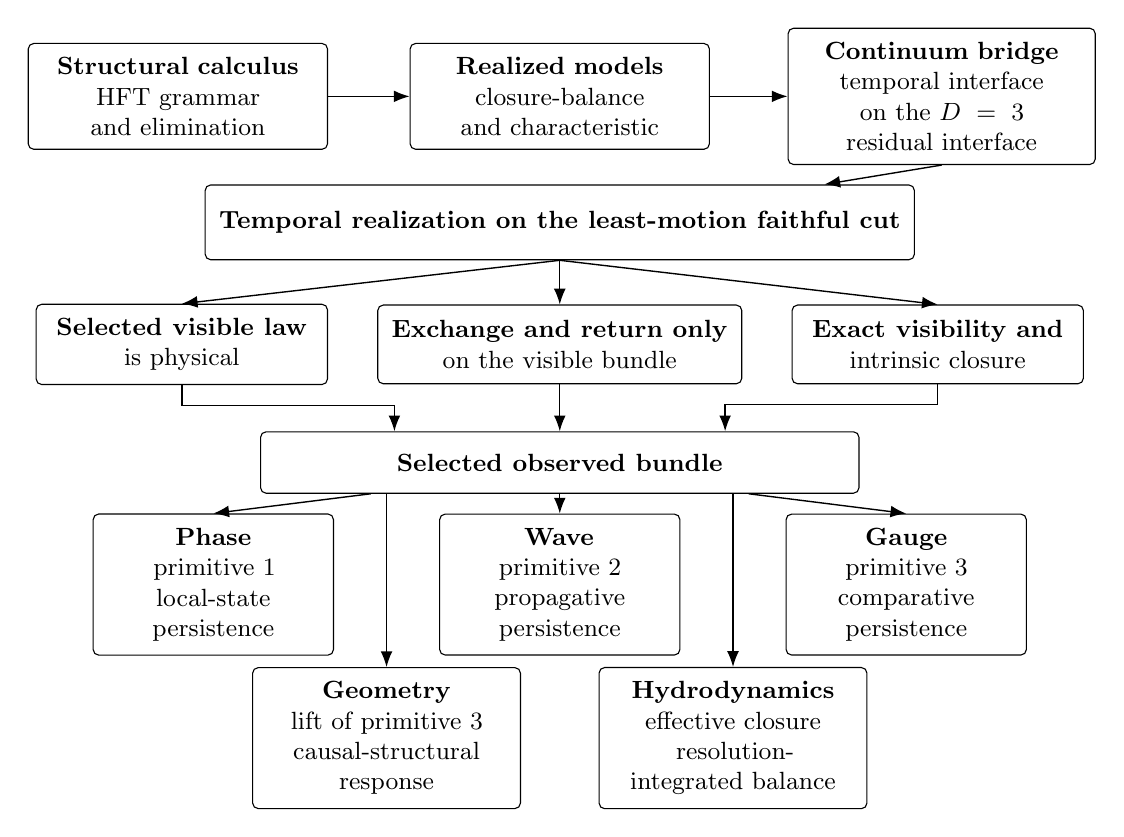
\begin{tikzpicture}[x=1cm,y=1cm]
  \node[ccbox, align=center, text width=3.45cm, minimum height=0.92cm] (p1) at (-4.85,5.15)
    {\textbf{Structural calculus}\\HFT grammar and elimination};
  \node[ccbox, align=center, text width=3.45cm, minimum height=0.92cm] (p2) at (0,5.15)
    {\textbf{Realized models}\\closure-balance and characteristic};
  \node[ccbox, align=center, text width=3.55cm, minimum height=0.92cm] (p3) at (4.85,5.15)
    {\textbf{Continuum bridge}\\temporal interface on the \(D=3\) residual interface};

  \draw[ccarrow, line width=0.5pt] (p1.east) -- (p2.west);
  \draw[ccarrow, line width=0.5pt] (p2.east) -- (p3.west);

  \node[ccbox, align=center, minimum width=5.6cm, minimum height=0.95cm] (realize) at (0,3.55)
    {\textbf{Temporal realization on the least-motion faithful cut}};
  \draw[ccarrow, line width=0.5pt]
    (p3.south) -- ($(realize.north east)+(-1.15,0)$);

  \node[ccbox, align=center, minimum width=3.7cm, minimum height=1.0cm] (law) at (-4.8,2.0)
    {\textbf{Selected visible law}\\is physical};
  \node[ccbox, align=center, minimum width=3.7cm, minimum height=1.0cm] (exchange) at (0,2.0)
    {\textbf{Exchange and return only}\\on the visible bundle};
  \node[ccbox, align=center, minimum width=3.7cm, minimum height=1.0cm] (closure) at (4.8,2.0)
    {\textbf{Exact visibility and}\\intrinsic closure};

  \draw[ccarrow, line width=0.5pt] (realize.south) -- (law.north);
  \draw[ccarrow, line width=0.5pt] (realize.south) -- (exchange.north);
  \draw[ccarrow, line width=0.5pt] (realize.south) -- (closure.north);

  \node[ccbox, align=center, minimum width=7.6cm, minimum height=0.78cm] (bundle) at (0,0.5)
    {\textbf{Selected observed bundle}};

  \draw[ccarrow, line width=0.5pt] (law.south) -- ++(0,-0.26) -| ($(bundle.north)+(-2.1,0)$);
  \draw[ccarrow, line width=0.5pt] (exchange.south) -- (bundle.north);
  \draw[ccarrow, line width=0.5pt] (closure.south) -- ++(0,-0.26) -| ($(bundle.north)+(2.1,0)$);

  \node[ccbox, align=center, text width=2.7cm, minimum height=1.15cm] (phase) at (-4.4,-1.05)
    {\textbf{Phase}\\primitive \(1\)\\local-state persistence};
  \node[ccbox, align=center, text width=2.7cm, minimum height=1.15cm] (wave) at (0,-1.05)
    {\textbf{Wave}\\primitive \(2\)\\propagative persistence};
  \node[ccbox, align=center, text width=2.7cm, minimum height=1.15cm] (gauge) at (4.4,-1.05)
    {\textbf{Gauge}\\primitive \(3\)\\comparative persistence};
  \node[ccbox, align=center, text width=3.05cm, minimum height=1.15cm] (geom) at (-2.2,-3.0)
    {\textbf{Geometry}\\lift of primitive \(3\)\\causal-structural response};
  \node[ccbox, align=center, text width=3.05cm, minimum height=1.15cm] (hydro) at (2.2,-3.0)
    {\textbf{Hydrodynamics}\\effective closure\\resolution-integrated balance};

  \draw[ccarrow, line width=0.5pt] ($(bundle.south)+(-2.4,0)$) -- (phase.north);
  \draw[ccarrow, line width=0.5pt] (bundle.south) -- (wave.north);
  \draw[ccarrow, line width=0.5pt] ($(bundle.south)+(2.4,0)$) -- (gauge.north);
  \draw[ccarrow, line width=0.5pt] ($(bundle.south)+(-2.2,0)$) -- (geom.north);
  \draw[ccarrow, line width=0.5pt] ($(bundle.south)+(2.2,0)$) -- (hydro.north);
\end{tikzpicture}%
}
\caption{Common physical pipeline. The structural horizon calculus, its
realized closure-balance and characteristic models, and the continuum bridge
at the end of Part~I feed the Part~II temporal realization law.
On the least-motion faithful cut the selected visible law is physical,
exchange and returned residual exhaust admissible forcing, and exact
visibility yields one selected observed bundle carrying the three primitive
direct channels, the canonical geometric lift of the primitive
\(3\)-channel, and the separate resolution-integrated hydrodynamic closure
lane.}
\label{fig:part-iv-common-pipeline}
\end{figure}

\begin{remark}[Bundle-level reading]
\label{rem:bundle-first-reading}\lean{SelectedBundle.FirstReading}
At the bundle level, one selects the faithful cut on which coherent visibility
persists, reads that ordered persistence as physical time, forms the exact
visible effective law on that cut, identifies all visible forcing as returned
residual, restricts visible sources to exchange-boundary reentry, reduces
unresolved bulk contribution to endpoint return, generates the canonical
visible carrier sectors, and classifies the surviving minimal compatible
closure on the associated visible carrier. In the canonical four-dimensional
realization of Part~II, this yields a common selected \(D=4\) observed bundle
together with a stable \(D=2\) phase sector as its smallest reversible
associated carrier.
\end{remark}

\subsection{Universal Consequences of Temporal Realization}

Before passing to carrier-level readouts, the temporal realization principle
already forces a universal physical layer. Some of these consequences are
immediate consequences of the law itself; others require the additional
variational or regularity hypotheses under which one ordinarily writes action
principles or continuous symmetry flows. They enter here as consequences of
temporal realization, not as unrelated primitive axioms.

\subsubsection{Causality}

\begin{theorem}[Temporal realization forces causal visible propagation]
\label{thm:temporal-realization-forces-causal-propagation}\lean{physical_realization_principle, residual_return_principle}
Assume the temporal realization principle on a selected cut. Then admissible
visible influence on that cut is causal in the following sense:
\begin{enumerate}[label=(\roman*), leftmargin=2em, itemsep=0.2em]
\item the visible dynamics are read on an ordered horizon family, so visible
      evolution is evaluated only along that realized order;
\item every admissible visible forcing term factors through returned residual
      propagated in the hidden or interface sector of the same coherent bundle;
\item no visible influence unsupported by that ordered propagation is
      admissible on the realized cut.
\end{enumerate}
In particular, on the physically realized cut there is no primitive acausal
visible action.
\end{theorem}

(Proof in Appendix~\ref{sec:appendix-dynamics}.)

\subsubsection{Stationarity and Action}

\begin{definition}[Stationary faithful temporal realization]
\label{def:stationary-faithful-temporal-realization}\lean{SelectedCut.GroundedBridge, observerMotionValue}
Fix a realized family and an admissible family of faithful characteristic cuts
that all carry the same persistent visible ordering. A faithful temporal
realization is \emph{stationary} if the observer-motion functional has zero
first variation at the realized cut along every admissible deformation through
that family. It is \emph{minimizing} if the realized cut attains the minimum of
that functional on the same admissible class.
\end{definition}

\begin{theorem}[Least-motion realization is stationary]
\label{thm:least-motion-realization-is-stationary}\lean{SelectedCut.groundedBridge, observerMotionValue_minimal}
Assume the temporal realization principle on a realized family, and assume the
admissible faithful cuts carrying the same persistent visible ordering form a
differentiable family on which the observer-motion functional is differentiable.
Then the physically realized least-motion cut is stationary in the sense of
Definition~\ref{def:stationary-faithful-temporal-realization}. If the least-
motion cut is unique, it is the unique minimizing stationary faithful
realization.
\end{theorem}

\begin{proof}
By the temporal realization principle, the physically realized cut is selected
as the unique least-motion cut among faithful cuts carrying the same ordered
persistent visible law. A differentiable minimizer of a differentiable
functional has vanishing first variation. Hence the realized cut is stationary.
If the least-motion cut is unique, it is also the unique minimizing stationary
realization on that admissible family.
\end{proof}

\subsubsection{Symmetry and Conservation}

\begin{corollary}[Stationary action on reversible realized sectors]
\label{cor:stationary-action-on-reversible-realized-sectors}\lean{PhaseLane.leastMotionObserver, WaveLane.leastMotionObserver, GaugeLane.leastMotionObserver, GeometricLane.leastMotionObserver}
Assume the setting of
Theorem~\ref{thm:least-motion-realization-is-stationary}. Suppose in addition
that on a reversible visible carrier the observer-motion functional is
represented on admissible histories by a differentiable action functional
\[
S[\phi].
\]
Then the physically realized history on that carrier satisfies
\[
\delta S = 0.
\]
If the action is local and regular, the corresponding Euler--Lagrange
equations are exactly the reversible carrier law on that realized sector.
\end{corollary}

\begin{proof}
By Theorem~\ref{thm:least-motion-realization-is-stationary}, the realized
history is stationary for the observer-motion functional. If that functional is
represented by the action \(S[\phi]\) on the reversible carrier, then the
first variation of \(S\) vanishes at the realized history. Under the standard
local regularity assumptions, vanishing of the first variation yields the
Euler--Lagrange equations. Thus stationary action is a reversible-sector form
of temporal realization rather than an extra primitive postulate.
\end{proof}

\begin{definition}[Temporal stabilizer symmetry]
\label{def:temporal-stabilizer-symmetry}\lean{RealizationSelectionPrinciple, EndogenousExchangeReturnPrinciple}
Fix a realized family satisfying the temporal realization principle on a
selected cut. A \emph{temporal stabilizer symmetry} is an admissible
transformation of the realized data that preserves:
\begin{enumerate}[label=(\roman*), leftmargin=2em, itemsep=0.2em]
\item the realized temporal class of faithful cuts up to horizon-preserving
      equivalence;
\item the selected visible effective law on that class;
\item the exchange / residual-return bookkeeping on that class;
\item the inherited endpoint closure class on the visible carrier under
      consideration.
\end{enumerate}
\end{definition}

\begin{theorem}[Physical symmetries are stabilizers of temporal realization]
\label{thm:physical-symmetries-are-temporal-stabilizers}\lean{realization_selection_principle}
Assume the temporal realization principle on a realized family. Then the
physical symmetries of the visible dynamics are exactly the admissible
transformations that stabilize the realized temporal structure in the sense of
Definition~\ref{def:temporal-stabilizer-symmetry}. In particular, symmetry is
not an extra declaration beside the law: it is the stabilizer of the
temporally realized coherent dynamics.
\end{theorem}

(Proof in Appendix~\ref{sec:appendix-dynamics}.)

\begin{theorem}[Noether-type bridge on temporally realized reversible sectors]
\label{thm:noether-bridge-on-temporally-realized-reversible-sectors}\lean{realization_selection_principle}
Assume the hypotheses of
Corollary~\ref{cor:stationary-action-on-reversible-realized-sectors}. Suppose
in addition that a one-parameter family of temporal stabilizer symmetries acts
smoothly on the admissible histories and preserves the action functional
\(S\). Then the realized reversible sector carries a conserved visible current
\(J\) satisfying
\[
\partial J = 0
\]
for the carrier-side boundary / divergence / codifferential operator
appropriate to that sector. Equivalently, the corresponding Noether charge is
constant along the realized temporal evolution.
\end{theorem}

(Proof in Appendix~\ref{sec:appendix-dynamics}.)

\subsubsection{Irreversibility}

\begin{theorem}[Temporal realization forbids primitive internal creation]
\label{thm:temporal-realization-forbids-primitive-internal-creation}\lean{endogenous_exchange_return_principle, coupled_exchange_balance}
Assume the temporal realization principle on a finite coupled family of visible
carriers on one selected bundle. Then every admissible visible source term is
an exchange term with another visible sector or with the hidden complement of
the same coherent bundle. In particular, a closed temporally realized system
has no net internal creation on the visible side.
\end{theorem}

\begin{proof}
This is exactly the exchange-balance clause of the temporal realization
principle. By that clause, visible sources are not primitive creations but
boundary readouts of internal exchange on the same coherent bundle. Therefore a
closed coupled visible system cannot carry net internal creation. The explicit
finite coupled cancellation formula is written below in
Theorem~\ref{thm:coupled-exchange-balance}.
\end{proof}

\begin{theorem}[Unrecovered residual orients physical time]
\label{thm:unrecovered-residual-orients-physical-time}\lean{SelectedCut.effectiveThermodynamicClosure, residual_return_principle}
Assume the temporal realization principle on a selected cut, and assume the
selected cut carries a quantitative unrecovered-residual functional whose
monotone part measures visible irreversibility. Then:
\begin{enumerate}[label=(\roman*), leftmargin=2em, itemsep=0.2em]
\item irreversible visible evolution is oriented by the monotone accumulation
      of unrecovered residual;
\item reversible realized sectors are exactly those on which no monotone
      unrecovered residual accumulates at the visible level;
\item the thermodynamic arrow of time is therefore not an extra primitive law,
      but the macroscopic reading of residual nonrecovery on the realized cut.
\end{enumerate}
\end{theorem}

\begin{proof}
By the temporal realization principle, observable irreversibility is exactly
unrecovered residual on the realized cut. If the selected cut carries a
quantitative unrecovered-residual functional whose monotone part measures that
irreversibility, then the direction of monotone increase determines the
orientation of irreversible visible evolution. Conversely, where no monotone
unrecovered residual accumulates, the visible law is reversible at the
realized level. Thus the arrow of time is read from residual nonrecovery on the
same cut on which physical time is realized.
\end{proof}

\subsubsection{Standard Structural Consequences}

The preceding results are intended to recover the standard structural backbone
of physics before any carrier-specific equation is recognized. To keep the
scope exact, the next proposition records only what has already been proved at
this universal level and distinguishes it from the later carrier-level
identification problem.

\begin{proposition}[Scoped recovery of standard physical principles]
\label{prop:scoped-recovery-of-standard-principles}\lean{physical_realization_principle, SelectedCut.effectiveThermodynamicClosure, coupled_exchange_balance}
Assume the temporal realization principle on a selected cut, together with the
additional hypotheses stated in the corresponding results above when required.
Then the following standard structural principles are recovered as
consequences of temporal realization:
\begin{enumerate}[label=(\roman*), leftmargin=2em, itemsep=0.2em]
\item \emph{Causal propagation / locality:}
      Theorem~\ref{thm:temporal-realization-forces-causal-propagation} shows
      that visible influence on the realized cut is causal and that no
      primitive acausal visible action is admissible.
\item \emph{Stationary realization / action principle:}
      Theorem~\ref{thm:least-motion-realization-is-stationary} and
      Corollary~\ref{cor:stationary-action-on-reversible-realized-sectors}
      show that least-motion temporal realization becomes stationary
      realization, and on reversible sectors with an action representation this
      yields the usual stationary-action form \(\delta S=0\).
\item \emph{Symmetry principle:}
      Theorem~\ref{thm:physical-symmetries-are-temporal-stabilizers} identifies
      physical symmetries with stabilizers of the temporally realized coherent
      dynamics.
\item \emph{Noether bridge:}
      Theorem~\ref{thm:noether-bridge-on-temporally-realized-reversible-sectors}
      shows that continuous temporal stabilizers of a stationary reversible
      sector yield conserved visible currents.
\item \emph{Conservation / exchange balance:}
      Theorem~\ref{thm:temporal-realization-forbids-primitive-internal-creation}
      shows that closed temporally realized systems carry no primitive visible
      creation, and that admissible visible sources are internal exchange or
      returned residual.
\item \emph{Arrow of time / irreversibility:}
      Theorem~\ref{thm:unrecovered-residual-orients-physical-time} shows that
      the macroscopic arrow of time is the monotone reading of unrecovered
      residual on the realized cut.
\end{enumerate}
These recovered principles are universal and carrier-generic. They do not yet
identify the canonical representatives of the phase, wave, kinetic, gauge, or
geometric endpoint classes. That further identification is the distinct
carrier-level task taken up below.
\end{proposition}

\begin{proof}
Each item is exactly the cited theorem or corollary. The final sentence records
the distinction between universal structural recovery and carrier-level
classification. The former has been proved in the present subsection; the
latter is deferred to the sector-generation and flagship layers that follow.
\end{proof}

\begin{remark}[Scope of universal recovery]
\label{rem:what-universal-recovery-does-not-claim}\lean{physical_realization_principle, flagship_law_completion}
The proposition above isolates a carrier-independent structural layer. It
recovers causal propagation, stationary realization, symmetry, Noether-type
conservation, exchange-balanced source admissibility, and irreversibility
before any carrier-specific endpoint equation is identified. The recognizable
Schr\"odinger, wave/Klein--Gordon, Maxwell, Einstein, and effective
hydrodynamic laws enter only after the carrier-level closure classes are
generated and their canonical representatives are identified.
\end{remark}


% --- Selected-cut framework and physical dynamics (continuation) ---



\manuscriptchapter{12}{Endpoint Completion, Carrier Realizations, and Classification}
\section{Endpoint Completion, Carrier Realizations, and Classification}
\label{sec:carrier-faces-and-completion}

Part~I proves the structural calculus and continuum bridge. Part~II assumes
the explicit three-law physical hypothesis and proves its carrier-level
consequences. On the selected cut, the common visible law and the
endpoint-complete microscopic structure have already been fixed by that
explicit Part~II hypothesis. The remaining questions are carrier-level: which
intrinsically generated sectors collapse to unique endpoint representatives,
which admit only canonical normal forms, and how the selected bundle closes
its present classification. This chapter answers those questions.

Its first task is endpoint rigidity, the last-step principle by which local
law candidates on an intrinsically generated carrier collapse to a unique
representative or to a canonical parameterized normal form. Its second task is
selected-cut completion and classification: on the present scope, the
selected bundle closes with three primitive direct laws, one unique geometric
lift, and effective closures above them. In particular, this chapter isolates
the complete fundamental set on the present scope and separates it from the
hydrodynamic and thermodynamic effective closures read on the same bundle.
It also identifies the predictive correction structure on the present scope:
returned remainders and induced scales on that same selected datum.

The chapter therefore assumes the Chapter~10 three-law hypothesis and the common
selected-cut structure of Chapter~11, and proves the carrier
identifications together with the scoped complete-fundamental-set theorem
directly from that explicit Part~II hypothesis.

\begin{tcolorbox}[colback=white, colframe=black!75, boxrule=0.9pt, title={Chapter 12 at a glance}]
\begin{description}[leftmargin=1.7em, itemsep=0.25em]
\item[Assumes.] The Chapter~10 three-law hypothesis and the Chapter~11
      selected-cut structure.
\item[Proves.] Endpoint-rigidity interfaces, the canonical carrier
      identifications, the scoped complete-fundamental-set theorem, the
      predictive correction structure carried by returned remainders and
      induced scales, and the separation between fundamental and effective
      laws on the present scope.
\item[Open.] The Chapter~10 endpoint-completion derivability question remains
      the only upstream law-side open problem carried into this chapter.
\end{description}
\end{tcolorbox}

\subsection{Endpoint Rigidity}

\begin{definition}[Endpoint rigidity principle]
\label{def:endpoint-rigidity-principle}\lean{EndpointRigidity.Principle}
Fix an intrinsically generated visible carrier on the selected cut. An
\emph{endpoint rigidity principle} for that carrier consists of the following
schema:
\begin{enumerate}[label=(\roman*), leftmargin=2em, itemsep=0.2em]
\item locality on the carrier is reduced to a finite closure class, in the
      spirit of finite-order jet reduction;
\item the generated carrier symmetries act on that finite closure class;
\item the carrier's compatibility identities cut the admissible operator space
      further;
\item an explicit endpoint-equivalence relation is fixed on that class;
\item minimal truncation / order / weight reduces the admissible quotient to a
      finite-dimensional space.
\end{enumerate}
If the resulting admissible quotient is singleton modulo endpoint
equivalence, the endpoint law is rigid and has a unique canonical
representative. If it is not singleton, the correct output is a
canonical normal form with explicit parameter data rather than false
uniqueness.
\end{definition}

\begin{remark}[Scope of endpoint rigidity]
\label{rem:endpoint-rigidity-schema}\lean{EndpointRigidity.Principle, EndpointRigidity.Principle.surface}
Definition~\ref{def:endpoint-rigidity-principle} is the common
``last-step'' shape suggested by the literature: local law candidates are
first reduced to a finite closure class, then symmetry and compatibility
collapse that space, and finally minimal truncation decides whether the
endpoint is rigid or merely canonical up to parameters. This is a common
method, not a single universal theorem that simultaneously yields
Schr\"odinger, wave/Klein--Gordon, Maxwell, Einstein, Navier--Stokes, and
thermodynamic semigroup forms. The actual collapse theorems remain
sector-specific.
\end{remark}

\begin{definition}[Realized-cut energy orthogonality]
\label{def:realized-cut-energy-orthogonality}\lean{SelectedCutOrthogonality.Principle}
Fix an intrinsically generated reversible visible carrier on the selected cut.
A \emph{realized-cut energy orthogonality datum} consists of:
\begin{enumerate}[label=(\roman*), leftmargin=2em, itemsep=0.2em]
\item the selected cut is \emph{energy-orthogonal}: the visible/shadow split
      satisfies an exact Pythagorean energy identity with no extra
      observer-induced remainder;
\item trial and test data are both read on that same selected visible carrier;
\item the selected-cut energy split induces a canonical pairing on that
      carrier;
\item the generated carrier symmetries and admissible endpoint operators
      preserve that endogenous pairing;
\item the weak law on that pairing determines a unique pairing-compatible
      strong representative.
\end{enumerate}
\end{definition}

\begin{theorem}[Canonical selected Schur bridge forces the exact selected-cut energy split]
\label{thm:canonical-selected-schur-bridge-forces-exact-selected-cut-energy-split}\lean{SelectedCutOrthogonality.exactSplit}
Fix a realized family satisfying a canonical selected Schur bridge on a
least-motion characteristic observer datum, and let \(\mathcal Y\) be an
intrinsically generated reversible visible carrier on the selected cut. Then:
\begin{enumerate}[label=(\alph*), leftmargin=2em, itemsep=0.2em]
\item the visible/shadow split on \(\mathcal Y\) satisfies an exact
      Pythagorean energy identity with no extra observer-induced remainder;
\item the weak visible law on \(\mathcal Y\) is read with trial and test data
      on that same carrier;
\item the selected-cut energy split induces a canonical pairing on
      \(\mathcal Y\).
\end{enumerate}
\end{theorem}

\begin{proof}
Because a canonical selected Schur bridge contains the exact Schur tower and
the HFT-2 energy tower on one and the same realized horizon tower,
Theorem~\ref{thm:HFT2-general} applies on that selected datum. Hence the
visible/shadow split on every generated reversible visible carrier of that
datum satisfies the exact Pythagorean identity, proving \emph{(a)}. By
Theorem~\ref{thm:canonical-selected-schur-realization}(c)--(e), the selected
visible law is exactly visible and read on that same selected cut by the one
selected visible effective law, so its weak visible law on
\(\mathcal Y\) has both trial and test data on \(\mathcal Y\). This proves
\emph{(b)}. Restricting the exact selected-cut energy split to
\(\mathcal Y\) therefore yields the canonical carrier-side pairing, proving
\emph{(c)}.
\end{proof}

\begin{definition}[Residual selected-cut duality rigidity]
\label{def:residual-selected-cut-duality-rigidity}\lean{CanonicalDuality.ResidualRigidity}
Fix an intrinsically generated reversible visible carrier on the selected cut.
A \emph{residual selected-cut duality rigidity datum} consists of:
\begin{enumerate}[label=(\roman*), leftmargin=2em, itemsep=0.2em]
\item the generated carrier symmetries preserve the exact selected-cut pairing
      on that carrier;
\item admissible endpoint operators are pairing-symmetric on the forced
      endpoint closure class;
\item the weak law on that pairing determines a unique pairing-compatible
      strong representative.
\end{enumerate}
\end{definition}

\begin{corollary}[Canonical selected Schur bridge plus residual duality rigidity forces realized-cut energy orthogonality]
\label{cor:canonical-selected-schur-bridge-plus-canonical-duality-forces-realized-cut-energy-orthogonality}\lean{SelectedCutOrthogonality.derived}
Fix a realized family satisfying a canonical selected Schur bridge on a
least-motion characteristic observer datum, and let \(\mathcal Y\) be an
intrinsically generated reversible visible carrier on the selected cut. Assume
in addition that \(\mathcal Y\) satisfies the residual selected-cut duality
rigidity datum of
Definition~\ref{def:residual-selected-cut-duality-rigidity}. Then \(\mathcal Y\)
satisfies the realized-cut energy orthogonality datum of
Definition~\ref{def:realized-cut-energy-orthogonality}.
\end{corollary}

\begin{proof}
Theorem~\ref{thm:canonical-selected-schur-bridge-forces-exact-selected-cut-energy-split}
gives items \emph{(i)}--\emph{(iii)} of
Definition~\ref{def:realized-cut-energy-orthogonality}. Definition~
\ref{def:residual-selected-cut-duality-rigidity} supplies the remaining
carrier-side duality clauses: its items \emph{(i)}--\emph{(ii)} give
preservation of the selected-cut pairing by the generated symmetries and
admissible endpoint operators, and its item \emph{(iii)} is exactly the
pairing-compatible strong representative clause. Thus all clauses of
Definition~\ref{def:realized-cut-energy-orthogonality} hold on
\(\mathcal Y\).
\end{proof}

\begin{theorem}[Canonical selected Schur bridge plus endpoint rigidity force endpoint substitution]
\label{thm:energy-orthogonal-cut-forces-canonical-duality}\lean{SelectedCutOrthogonality.forcesEndpointSubstitution}
Fix a realized family satisfying a canonical selected Schur bridge on a
least-motion characteristic observer datum, and let \(\mathcal Y\) be an
intrinsically generated reversible visible carrier on the selected cut. Assume
the endpoint closure class on \(\mathcal Y\) is already unique modulo
continuum equivalence. Then the final carrier-level representative is fixed
internally: the exact selected-cut energy split supplies the canonical
pairing, and the pairing-compatible strong representative is forced by the
weak law. In particular, the last representative substitution is no longer a
discretionary recognition step.
\end{theorem}

\begin{proof}
By
Theorem~\ref{thm:canonical-selected-schur-bridge-forces-exact-selected-cut-energy-split},
the exact selected-cut Pythagorean identity holds on \(\mathcal Y\), trial and
test data are both read on that same generated carrier, and the selected-cut
energy split induces the canonical pairing on \(\mathcal Y\). Once
endpoint-rigidity has already reduced the admissible closure class on
\(\mathcal Y\) to a unique continuum-equivalence class, any strong
representative compatible with that weak law and that canonical pairing must
lie in that one class. Hence the weak law has only one pairing-compatible
strong representative left, so the endpoint substitution is forced internally
by the exact selected-cut energy split.
\end{proof}

\begin{remark}[Canonical duality as derived interface]
\label{rem:canonical-duality-derived}\lean{SelectedCutOrthogonality.Principle, SelectedCutOrthogonality.Principle.surface}
Definition~\ref{def:realized-cut-energy-orthogonality} is the more structural
statement. The earlier ``canonical duality'' language is still useful, but it
is a \emph{derived interface} extracted from exact selected-cut energy
bookkeeping rather than a separate primitive hypothesis.
\end{remark}

\begin{definition}[Canonical duality sector rigidity]
\label{def:canonical-duality-sector-rigidity}\lean{CanonicalDuality.SectorRigidity}
Fix an intrinsically generated reversible visible carrier on the selected cut.
A \emph{canonical duality sector rigidity datum} consists of:
\begin{enumerate}[label=(\roman*), leftmargin=2em, itemsep=0.2em]
\item trial and test data generated by that same visible carrier;
\item a canonical pairing identifying those trial and test data;
\item preservation of that pairing by the generated carrier symmetries;
\item admissible endpoint operators that are pairing-symmetric on the forced
      endpoint closure class;
\item a weak formulation whose canonical pairing determines a unique strong
      representative.
\end{enumerate}
\end{definition}

\begin{theorem}[Canonical duality forces endpoint substitution]
\label{thm:canonical-duality-forces-endpoint-substitution}\lean{CanonicalDuality.SectorRigidity.forcesEndpointSubstitution}
Assume a generated reversible visible carrier satisfies
Definition~\ref{def:canonical-duality-sector-rigidity}, and that its endpoint
closure class is already unique modulo continuum equivalence. Then the final
carrier-level substitution is not a free choice by the practitioner: the weak
law on that carrier determines a unique strong canonical representative. This
is the derived duality-interface form of
Theorem~\ref{thm:energy-orthogonal-cut-forces-canonical-duality}.
\end{theorem}

\begin{proof}
Definition~\ref{def:canonical-duality-sector-rigidity} identifies trial and
test data on one and the same generated visible carrier, equips them with a
canonical pairing, and restricts admissible endpoint operators to the
pairing-symmetric representatives of the already forced endpoint closure
class. Once uniqueness modulo continuum equivalence is already available from
the endpoint-rigidity reduction, the weak formulation has only one compatible
strong representative left. Hence the final representative substitution is
forced internally.
\end{proof}

\begin{remark}[Where this applies]
\label{rem:canonical-duality-sector-rigidity}\lean{CanonicalDuality.SectorRigidity, CanonicalDuality.SectorRigidity.surface}
Theorem~\ref{thm:canonical-duality-forces-endpoint-substitution} is the common
intrinsic-sector mechanism behind the final representative identification on
the phase, wave, gauge, and geometric carriers. It is \emph{not} the right
last-step mechanism for the hydrodynamic or thermodynamic realizations, where
one expects canonical normal forms with transport or entropy-production data
rather than the same self-dual rigidity.
\end{remark}

\begin{remark}[The exact remaining intrinsic-sector obligations]
\label{rem:remaining-intrinsic-endpoint-obligations}\lean{NaturalOperatorCompletion, NaturalOperatorCompletion.guidedByEndpointRigidity}
Theorem~\ref{thm:energy-orthogonal-cut-forces-canonical-duality} removes the
discretionary final substitution step once the endpoint class on a reversible
carrier is already rigid modulo continuum equivalence. Moreover, the
singleton/uniqueness side of the endpoint quotient is already isolated by the
common endpoint-rigidity reduction. Accordingly, the intrinsic endpoint
question reduces to carrier-specific collapse of the already forced singleton
endpoint class to the familiar named representative. All four intrinsic
representative collapses are discharged on the phase, wave, gauge, and
geometric laws by Theorems~\ref{thm:phase-local-endpoint-collapse} and
\ref{thm:wave-local-endpoint-collapse}, together with
Theorem~\ref{thm:gauge-local-endpoint-collapse} and
Theorem~\ref{thm:geometric-local-endpoint-collapse}. The optional exact
constant-mass Klein--Gordon refinement is likewise proved on homogeneous
selected-wave sectors by
Theorem~\ref{thm:homogeneous-wave-scalar-profile-forces-constant-mass}.
\end{remark}

\begin{remark}[Sharper carrier-level frontiers]
\label{rem:active-intrinsic-frontier}\lean{FlagshipLawCompletion, flagship_law_completion}
The common reductions now push each intrinsic carrier to a sharp closed
structural frontier.
On the phase carrier, the complex generator is fixed internally and the local
Laplace/potential collapse is isolated by
Theorem~\ref{thm:phase-local-endpoint-collapse}. On the wave carrier, the local
Laplace/scalar-profile collapse is isolated by
Theorem~\ref{thm:wave-local-endpoint-collapse}, and the exact constant-mass
Klein--Gordon refinement is proved on homogeneous selected-wave sectors by
Theorem~\ref{thm:homogeneous-wave-scalar-profile-forces-constant-mass}. On the
gauge carrier, the intrinsic curvature-adjoint collapse is proved by
Theorem~\ref{thm:gauge-local-endpoint-collapse}, and the recognizable Maxwell
form is Corollary~\ref{cor:recognizable-maxwell-identity}. On the geometric
carrier, the intrinsic trace-adjusted curvature collapse is proved by
Theorem~\ref{thm:geometric-local-endpoint-collapse}, and the recognizable
Einstein form is Corollary~\ref{cor:recognizable-einstein-identity}. Thus
the remaining
carrier-specific burden is now narrower still: it is not basic equation
recognition on the intrinsic laws, but downstream bridge and effective-closure
questions outside those already closed structural frontiers.
\end{remark}

\begin{definition}[Exchange-balanced coupled family]
\label{def:exchange-balanced-coupled-family}\lean{ExchangeBalancedCoupledFamily}
Fix a finite family of associated visible carriers
\(\{\mathcal X_h^\alpha\}_{\alpha\in A}\) on one selected observed bundle. A
family of visible source terms \(\{S_\alpha\}_{\alpha\in A}\) on these carriers
is an \emph{exchange-balanced coupled family} if there exist pairwise exchange
currents or tensors \(J_{\alpha\beta}\) such that, for all distinct
\(\alpha,\beta\in A\),
\[
J_{\alpha\beta}=-J_{\beta\alpha},
\qquad
S_\alpha=\sum_{\beta\in A\setminus\{\alpha\}} \partial J_{\alpha\beta},
\]
where \(\partial\) denotes the carrier-side boundary, divergence, or
codifferential map appropriate to the visible carrier.
\end{definition}

\begin{theorem}[Coupled exchange balance]
\label{thm:coupled-exchange-balance}\lean{coupled_exchange_balance}
Let \(\{S_\alpha\}_{\alpha\in A}\) be an exchange-balanced coupled family on a
finite collection of selected visible carriers. Then
\[
\sum_{\alpha\in A} S_\alpha = 0.
\]
Equivalently, a closed coupled selected system has zero net internal creation.
In the two-carrier case \(A=\{X,Y\}\), one has
\[
S_X=-S_Y,
\]
so localized equal-and-opposite interaction is the two-endpoint specialization
of the general exchange law.
\end{theorem}

(Proof in Appendix~\ref{sec:appendix-dynamics}.)

\begin{remark}[Consequences for coupled carriers]\lean{coupled_exchange_balance}
\label{rem:what-coupled-exchange-collapses}
Theorem~\ref{thm:coupled-exchange-balance} is the common physical source law
beneath the carrier-specific laws. On the kinetic carrier it identifies
production as exchange with unresolved higher moments; on the gauge carrier it
identifies the visible one-form \(J\) as an exchange current; on the geometric
carrier it identifies the visible tensor \(T\) as an exchange tensor. In the
localized two-endpoint limit it reduces to equal-and-opposite interaction.
\end{remark}

\subsection{Selected-Cut Completion}

Definitions~\ref{def:grounded-physical-bridge} and
\ref{def:localized-residual-return} are retained as auxiliary bridge readouts:
they unpack the least-motion grounding clause and the return-field /
irreversibility clause separately. The actual completion chain used in
Theorem~\ref{thm:part-iv-law-completion} starts with the canonical selected
Schur bridge of Definition~\ref{def:canonical-selected-schur-bridge}.

\begin{definition}[Grounded physical bridge]
\label{def:grounded-physical-bridge}\lean{SelectedCut.GroundedBridge}
A realized family satisfies the \emph{grounded physical bridge} condition if
the temporal realization principle is not left as a bare interpretive
identification, but is forced by a concrete observer-motion criterion on
admissible cuts: there is a defined observer-motion functional, the physically
realized cut is its unique least-motion faithful minimizer, and the selected
visible effective law on that minimizing cut is exactly the observable law.
\end{definition}

\begin{definition}[Localized residual return]
\label{def:localized-residual-return}\lean{SelectedCut.LocalizedReturn}
A grounded bridge satisfies \emph{localized residual return} if the residual
return calculus of the earlier structural chapters together with the continuum
bridge is promoted to an explicit residual return
field on the selected cut, that field is the one whose elimination gives the
selected visible effective law, it localizes on the unique residual interface
\(D=3\) in the canonical nontrivial realization, and there is a quantitative
unrecovered-residual functional whose monotone part measures observable
irreversibility.
\end{definition}

\begin{definition}[Intrinsic selected-bundle existence]
\label{def:intrinsic-selected-bundle-existence}\lean{IntrinsicSelectedBundleExistence}
A canonical selected Schur bridge satisfies
\emph{intrinsic selected-bundle existence} if the phase, wave, gauge, and
geometric carriers arise directly as associated visible carriers of one
physically realized selected observed bundle on the least-motion cut, without
separate carrier-wise visibility hypotheses.
\end{definition}

\begin{definition}[Schur-induced mode candidate class]
\label{def:schur-induced-mode-candidate-class}\lean{SchurInducedModeCandidateClass}
Fix a realized family satisfying a canonical selected Schur bridge on a
least-motion characteristic observer datum with selected observed bundle
\[
\mathcal X_h=P_h\cH^\bullet
\]
and canonical admissible realized class
\(\mathfrak R_{\mathrm{sel}}(h)\). Fix one persistence mode \(\mathfrak m\) of
Definition~\ref{def:five-persistence-modes}. The \emph{Schur-induced mode
candidate class} for \(\mathfrak m\) is the subclass
\[
\mathfrak R^{\mathrm{Schur}}_{\mathfrak m}(h)\subseteq
\mathfrak R_{\mathrm{sel}}(h)
\]
consisting of those realizations \(R\) for which, after transporting the
selected datum of \(R\) to \(\mathcal X_h\) by the horizon-preserving
equivalence supplied by the canonical selected Schur bridge, there is a visible
subcarrier \(\mathcal Y_R\subseteq \mathcal X_h\) such that:
\begin{enumerate}[label=(\roman*), leftmargin=2em, itemsep=0.2em]
\item \(\mathcal Y_R\) is faithful, reconstruction-compatible,
      closure-admissible, and stable under admissible promotion;
\item the restriction of the selected visible effective law to
      \(\mathcal Y_R\) preserves the compatibility signature and admissible
      source profile of the mode \(\mathfrak m\);
\item no proper visible subcarrier of \(\mathcal Y_R\) still satisfies
      \emph{(i)}--\emph{(ii)} for the same mode \(\mathfrak m\).
\end{enumerate}
Equivalently, \(\mathfrak R^{\mathrm{Schur}}_{\mathfrak m}(h)\) is the
intrinsic mode-selection problem cut out by the canonical selected Schur bridge
inside its own admissible realized class.
\end{definition}

\begin{theorem}[Nonempty Schur-induced mode classes have singleton reduced selection]
\label{thm:nonempty-schur-induced-mode-classes-have-singleton-reduced-selection}\lean{SchurInducedModeCandidateClass.singletonReducedSelection}
Fix a realized family satisfying a canonical selected Schur bridge on a
least-motion characteristic observer datum with selected observed bundle
\(\mathcal X_h=P_h\cH^\bullet\), and fix one persistence mode
\(\mathfrak m\). Assume the Schur-induced mode candidate class
\(\mathfrak R^{\mathrm{Schur}}_{\mathfrak m}(h)\) of
Definition~\ref{def:schur-induced-mode-candidate-class} is nonempty. Then:
\begin{enumerate}[label=(\roman*), leftmargin=2em, itemsep=0.2em]
\item \(\mathfrak R^{\mathrm{Schur}}_{\mathfrak m}(h)\) determines a
      mode-compatible candidate class on the selected cut in the sense of
      Definition~\ref{def:mode-compatible-candidate-class};
\item the admissible reduced selection data on
      \(\mathfrak R^{\mathrm{Schur}}_{\mathfrak m}(h)\), modulo
      horizon-preserving equivalence, consist of a single equivalence class;
\item the persistence mode \(\mathfrak m\) therefore has a unique least-motion
      visible realization on the selected cut.
\end{enumerate}
\end{theorem}

(Proof in Appendix~\ref{sec:appendix-dynamics}.)

\begin{theorem}[Intrinsic selected-channel data force nonemptiness of the local-state, propagative, and comparative Schur-induced mode classes]
\label{thm:intrinsic-selected-channel-package-forces-three-schur-mode-classes}\lean{IntrinsicSectorGeneration.threeSchurModeClasses}
Fix a realized family satisfying a canonical selected Schur bridge on a
least-motion characteristic observer datum with selected observed bundle
\[
\mathcal X_h=P_h\cH^\bullet
\]
and canonical admissible realized class \(\mathfrak R_{\mathrm{sel}}(h)\).
Assume:
\begin{enumerate}[label=(\roman*), leftmargin=2em, itemsep=0.2em]
\item \(\mathfrak R_{\mathrm{sel}}(h)\) satisfies the hypotheses of
      Corollary~\ref{cor:intrinsic-package-implies-governing-datum-rigid};
\item the relevant selected channels carry selected channel transport systems
      in the sense of Definition~\ref{def:selected-channel-transport-system}.
\end{enumerate}
Then the Schur-induced mode candidate classes for:
\begin{enumerate}[label=(\alph*), leftmargin=2em, itemsep=0.2em]
\item local-state persistence,
\item propagative persistence,
\item comparative persistence
\end{enumerate}
are all nonempty.
\end{theorem}

(Proof in Appendix~\ref{sec:appendix-dynamics}.)

\begin{definition}[Orthogonal Schur-lifted symmetric-response datum]
\label{def:orthogonal-schur-lifted-symmetric-response-package}\lean{GeometricWitness.OrthogonalPackage}
Fix a realized family satisfying a canonical selected Schur bridge on a
least-motion characteristic observer datum with selected observed bundle
\[
\mathcal X_h=P_h\cH^\bullet
\]
and canonical admissible realized class \(\mathfrak R_{\mathrm{sel}}(h)\). An
\emph{orthogonal Schur-lifted symmetric-response datum} on the selected cut
consists of:
\begin{enumerate}[label=(\roman*), leftmargin=2em, itemsep=0.2em]
\item a realization \(R_\ast\in\mathfrak R_{\mathrm{sel}}(h)\) and a relevant
      selected channel fiber \(F_h\) of \(R_\ast\) with \(\dim F_h\ge 2\);
\item a visible subcarrier
      \[
      \mathcal X_h^{\mathrm{sym}}\subseteq \mathcal X_h
      \]
      which, after transporting the selected datum of \(R_\ast\) to the common
      selected bundle by the horizon-preserving equivalence of the canonical
      selected Schur bridge, is identified with the symmetric-square carrier
      \(\mathrm{Sym}^2(F_h)\);
\item faithfulness, reconstruction compatibility, closure admissibility, and
      admissible-promotion stability of
      \(\mathcal X_h^{\mathrm{sym}}\) on the selected cut;
\item a divergence-compatible second-order response operator on
      \(\mathcal X_h^{\mathrm{sym}}\) induced by the selected visible effective
      law together with the canonical Schur return field;
\item equivariance of that induced response for the orthogonal conjugation
      action of \(O(F_h)\) on \(\mathrm{Sym}^2(F_h)\);
\item visible source on \(\mathcal X_h^{\mathrm{sym}}\) belonging to an
      exchange-balanced coupled family and represented by a symmetric exchange
      tensor furnished by preceding selected carriers on the same selected
      bundle;
\item no proper visible subcarrier of \(\mathcal X_h^{\mathrm{sym}}\) still
      supports the same divergence-compatible second-order response signature
      with the same exchange-source profile at the observed scale.
\end{enumerate}
\end{definition}

\begin{definition}[Schur-lifted symmetric-square response datum]
\label{def:schur-lifted-symmetric-square-response-package}\lean{GeometricWitness.SquarePackage}
Fix a realized family satisfying a canonical selected Schur bridge on a
least-motion characteristic observer datum with selected observed bundle
\[
\mathcal X_h=P_h\cH^\bullet
\]
and canonical admissible realized class \(\mathfrak R_{\mathrm{sel}}(h)\). A
\emph{Schur-lifted symmetric-square response datum} on the selected cut
consists of:
\begin{enumerate}[label=(\roman*), leftmargin=2em, itemsep=0.2em]
\item a realization \(R_\ast\in\mathfrak R_{\mathrm{sel}}(h)\) and a relevant
      selected channel fiber \(F_h\) of \(R_\ast\) with \(\dim F_h\ge 2\);
\item a visible subcarrier
      \[
      \mathcal X_h^{\mathrm{sym}}\subseteq \mathcal X_h
      \]
      which, after transporting the selected datum of \(R_\ast\) to the common
      selected bundle by the horizon-preserving equivalence of the canonical
      selected Schur bridge, is identified with the symmetric-square carrier
      \(\mathrm{Sym}^2(F_h)\);
\item faithfulness, reconstruction compatibility, closure admissibility, and
      admissible-promotion stability of
      \(\mathcal X_h^{\mathrm{sym}}\) on the selected cut;
\item a divergence-compatible second-order response operator on
      \(\mathcal X_h^{\mathrm{sym}}\) induced by the selected visible effective
      law together with the canonical Schur return field;
\item visible source on \(\mathcal X_h^{\mathrm{sym}}\) belonging to an
      exchange-balanced coupled family and represented by a symmetric exchange
      tensor furnished by preceding selected carriers on the same selected
      bundle;
\item no proper visible subcarrier of \(\mathcal X_h^{\mathrm{sym}}\) still
      supports the same divergence-compatible second-order response signature
      with the same exchange-source profile at the observed scale.
\end{enumerate}
\end{definition}

\begin{theorem}[Schur-lifted symmetric-square response forces the geometric witness]
\label{thm:schur-lifted-symmetric-square-response-forces-geometric-witness}\lean{GeometricWitness.square_geometricWitness}
Fix a realized family satisfying a canonical selected Schur bridge on a
least-motion characteristic observer datum with selected observed bundle
\[
\mathcal X_h=P_h\cH^\bullet.
\]
Assume the selected cut carries a Schur-lifted symmetric-square response
datum in the sense of
Definition~\ref{def:schur-lifted-symmetric-square-response-package}. Then the
selected bundle satisfies the hypotheses of
Theorem~\ref{thm:macroscopic-witness-packages-force-two-schur-mode-classes}.
Consequently the causal-structural Schur-induced mode candidate class on the
selected bundle is nonempty.
\end{theorem}

(Proof in Appendix~\ref{sec:appendix-dynamics}.)

\begin{corollary}[Orthogonal Schur-lifted symmetric response is a special case]
\label{cor:orthogonal-schur-lifted-symmetric-response-is-special-case}\lean{GeometricWitness.orthogonal_toSquare}
Fix a realized family satisfying a canonical selected Schur bridge on a
least-motion characteristic observer datum with selected observed bundle
\[
\mathcal X_h=P_h\cH^\bullet.
\]
Assume the selected cut carries an orthogonal Schur-lifted
symmetric-response datum in the sense of
Definition~\ref{def:orthogonal-schur-lifted-symmetric-response-package}. Then
the selected cut carries a Schur-lifted symmetric-square response datum in
the sense of
Definition~\ref{def:schur-lifted-symmetric-square-response-package}.
\end{corollary}

\begin{proof}
Every clause of
Definition~\ref{def:schur-lifted-symmetric-square-response-package} is already
contained in
Definition~\ref{def:orthogonal-schur-lifted-symmetric-response-package}; the
orthogonal-equivariance clause there is an additional refinement rather than an
extra burden for the weaker datum.
\end{proof}

\begin{theorem}[Orthogonal Schur-lifted symmetric response forces the geometric witness]
\label{thm:orthogonal-schur-lifted-symmetric-response-forces-geometric-witness}\lean{GeometricWitness.orthogonal_geometricWitness}
Fix a realized family satisfying a canonical selected Schur bridge on a
least-motion characteristic observer datum with selected observed bundle
\[
\mathcal X_h=P_h\cH^\bullet.
\]
Assume the selected cut carries an orthogonal Schur-lifted
symmetric-response datum in the sense of
Definition~\ref{def:orthogonal-schur-lifted-symmetric-response-package}. Then
the selected bundle satisfies the hypotheses of
Theorem~\ref{thm:macroscopic-witness-packages-force-two-schur-mode-classes}.
Consequently the causal-structural Schur-induced mode candidate class on the
selected bundle is nonempty.
\end{theorem}

\begin{proof}
By
Corollary~\ref{cor:orthogonal-schur-lifted-symmetric-response-is-special-case},
the stated orthogonal datum already yields a Schur-lifted symmetric-square
response datum. The conclusion is therefore exactly
Theorem~\ref{thm:schur-lifted-symmetric-square-response-forces-geometric-witness}.
\end{proof}

\begin{corollary}[Schur-lifted symmetric-square response closes the intrinsic mode-existence gap]
\label{cor:orthogonal-schur-lifted-symmetric-response-closes-mode-gap}\lean{GeometricWitness.orthogonal_closesModeGap}
Fix a realized family satisfying a canonical selected Schur bridge on a
least-motion characteristic observer datum. Assume:
\begin{enumerate}[label=(\roman*), leftmargin=2em, itemsep=0.2em]
\item the hypotheses of
      Theorem~\ref{thm:intrinsic-selected-channel-package-forces-three-schur-mode-classes};
\item the selected cut carries a Schur-lifted symmetric-square response
      datum in the sense of
      Definition~\ref{def:schur-lifted-symmetric-square-response-package}.
\end{enumerate}
Then intrinsic selected-bundle existence holds on the selected cut. If, in
addition, the remaining hypotheses of
Theorem~\ref{thm:single-witness-intrinsic-flagship-forcing} are also assumed,
then the four intrinsic law classes are forced on that bundle.
\end{corollary}

(Proof in Appendix~\ref{sec:appendix-dynamics}.)

\begin{theorem}[Phase, wave, and gauge law classes are already forced on the selected bundle]
\label{thm:first-three-intrinsic-law-classes-already-forced}\lean{NaturalOperatorCompletion.firstThreeClasses}
Fix a realized family satisfying a canonical selected Schur bridge on a
least-motion characteristic observer datum. Assume:
\begin{enumerate}[label=(\roman*), leftmargin=2em, itemsep=0.2em]
\item the hypotheses of
      Theorem~\ref{thm:intrinsic-selected-channel-package-forces-three-schur-mode-classes};
\end{enumerate}
Then:
\begin{enumerate}[label=(\alph*), leftmargin=2em, itemsep=0.2em]
\item the phase, wave, and gauge carriers arise on the selected bundle as the
      canonical minimal compatible realizations of local-state,
      propagative, and comparative persistence;
\item on each of these three carriers, the selected endpoint closure class is
      unique modulo continuum equivalence and is determined entirely by scalar
      data on the intrinsic symmetry channels of that carrier;
\item the remaining intrinsic burden on these three carriers is only the
      carrier-level representative collapse:
      phase/Laplace/potential, wave/Klein--Gordon, and
      the intrinsic gauge curvature-adjoint representative.
\end{enumerate}
\end{theorem}

(Proof in Appendix~\ref{sec:appendix-dynamics}.)

\begin{theorem}[The three primitive channels are already forced]
\label{thm:three-primitive-channels-already-forced}\lean{IntrinsicSectorGeneration.primitiveChannels}
Fix a realized family satisfying a canonical selected Schur bridge on a
least-motion characteristic observer datum. Assume the hypotheses of
Theorem~\ref{thm:first-three-intrinsic-law-classes-already-forced}. Then:
\begin{enumerate}[label=(\roman*), leftmargin=2em, itemsep=0.2em]
\item local-state, propagative, and comparative persistence are already forced
      on the selected bundle as the three primitive direct channels of the
      intrinsic \(1+2+3\) channel algebra;
\item their unique canonical direct visible realizations are exactly the
      phase, wave, and gauge carriers on that bundle;
\item within the current intrinsic family there is no fourth primitive
      channel.
\end{enumerate}
\end{theorem}

(Proof in Appendix~\ref{sec:appendix-dynamics}.)

\begin{corollary}[Geometry is the only remaining intrinsic lift/existence law]
\label{cor:geometry-only-remaining-intrinsic-existence-lane}\lean{IntrinsicSectorGeneration.remainingGeometricLane}
Fix a realized family satisfying a canonical selected Schur bridge on a
least-motion characteristic observer datum. Assume the hypotheses of
Theorem~\ref{thm:three-primitive-channels-already-forced}. Then the
intrinsic work separates as follows:
\begin{enumerate}[label=(\roman*), leftmargin=2em, itemsep=0.2em]
\item the phase, wave, and gauge laws are already reduced to their
      carrier-level representative collapses;
\item the geometric law, now understood as the unique intrinsic lift of the
      primitive \(3\)-channel, still requires one intrinsic existence theorem,
      namely a Schur-lifted symmetric-square response datum on the selected
      cut, or more primitively a faithful six-dimensional symmetric bilinear
      visible self-coupling of the primitive \(3\)-channel that factors
      through that symmetric-square lift, after which its remaining burden is
      only the
      trace-adjusted-Ricci / Einstein representative collapse.
\end{enumerate}
\end{corollary}

(Proof in Appendix~\ref{sec:appendix-dynamics}.)

\begin{theorem}[Carrier-by-carrier intrinsic closure frontier]
\label{thm:lane-by-lane-intrinsic-closure-frontier}\lean{FlagshipLawCompletion.laneByLaneClosureFrontier}
Fix a realized family satisfying a canonical selected Schur bridge on a
least-motion characteristic observer datum. Assume the hypotheses of
Theorem~\ref{thm:first-three-intrinsic-law-classes-already-forced}. Then the
four intrinsic laws separate exactly as follows:
\begin{enumerate}[label=(\roman*), leftmargin=2em, itemsep=0.2em]
\item \textbf{Phase.} The phase law class is already forced on the selected
      bundle. The complex phase generator is fixed by
      Theorem~\ref{thm:phase-generation-and-energy-orthogonality-force-complex-generator},
      and the local Laplace/potential collapse is proved by
      Theorem~\ref{thm:phase-local-endpoint-collapse}. Thus the recognizable
      Schr\"odinger identity is already closed at this level.
\item \textbf{Wave.} The wave law class is already forced on the selected
      bundle. Its local Laplace/scalar-profile collapse is proved by
      Theorem~\ref{thm:wave-local-endpoint-collapse}. The recognizable
      wave/Klein--Gordon notation of
      Corollary~\ref{cor:recognizable-wave-kg-identity} is then a further
      refinement when the forced real scalar profile is written with a
      distinguished constant mass datum, and the exact constant-mass
      Klein--Gordon refinement is proved on homogeneous selected-wave sectors
      by
      Theorem~\ref{thm:homogeneous-wave-scalar-profile-forces-constant-mass}
      and Corollary~\ref{cor:exact-recognizable-klein-gordon-identity}.
\item \textbf{Gauge.} The gauge law class is already forced on the selected
      bundle. Its intrinsic curvature-adjoint collapse is proved by
      Theorem~\ref{thm:gauge-local-endpoint-collapse}, and its recognizable
      Maxwell form is Corollary~\ref{cor:recognizable-maxwell-identity}.
\item \textbf{Geometry.} The geometric law class is already forced on the
      selected bundle as the unique intrinsic lift of the primitive
      \(3\)-channel. Its intrinsic trace-adjusted curvature collapse is proved
      by Theorem~\ref{thm:geometric-local-endpoint-collapse}, and its
      recognizable Einstein form is
      Corollary~\ref{cor:recognizable-einstein-identity}.
\end{enumerate}
\end{theorem}

(Proof in Appendix~\ref{sec:appendix-dynamics}.)

\begin{theorem}[Symmetric-response witness data force nonemptiness of the causal-structural Schur-induced mode class]
\label{thm:macroscopic-witness-packages-force-two-schur-mode-classes}\lean{GeometricWitness.square_closesModeGap}
Fix a realized family satisfying a canonical selected Schur bridge on a
least-motion characteristic observer datum with selected observed bundle
\[
\mathcal X_h=P_h\cH^\bullet.
\]
Assume \(\mathcal X_h\) carries a faithful, reconstruction-compatible,
closure-admissible, admissible-promotion-stable visible symmetric-response
subcarrier \(\mathcal X_h^{\mathrm{geom}}\) on which divergence-compatible
second-order response is visible and no proper visible subcarrier still
supports that same response signature at the observed scale. Then the
Schur-induced mode candidate class for causal-structural persistence is
nonempty.
\end{theorem}

(Proof in Appendix~\ref{sec:appendix-dynamics}.)

\begin{corollary}[Intrinsic selected-channel data plus symmetric-response witness force nonemptiness of all four Schur-induced mode classes]
\label{cor:intrinsic-package-plus-macroscopic-witnesses-force-five-schur-nonempty}\lean{FlagshipLawCompletion.fiveSchurNonempty}
Fix a realized family satisfying a canonical selected Schur bridge on a
least-motion characteristic observer datum. Assume the hypotheses of
Theorem~\ref{thm:intrinsic-selected-channel-package-forces-three-schur-mode-classes}
and
Theorem~\ref{thm:macroscopic-witness-packages-force-two-schur-mode-classes}.
Then all four Schur-induced mode candidate classes on the selected bundle are
nonempty.
\end{corollary}

\begin{proof}
The first theorem gives nonemptiness of the local-state, propagative, and
comparative Schur-induced mode classes. The second gives nonemptiness of the
causal-structural Schur-induced mode class. These are exactly the three
primitive persistence channels together with the geometric lift of
Definition~\ref{def:five-persistence-modes}.
\end{proof}

\begin{theorem}[Four nonempty Schur-induced mode classes force canonical realization of persistence modes]
\label{thm:four-nonempty-schur-induced-mode-classes-force-canonical-realization}\lean{SelectedBundle.CanonicalGeneration.fourSchurNonempty}
Fix a realized family satisfying a canonical selected Schur bridge on a
least-motion characteristic observer datum with selected observed bundle
\[
\mathcal X_h=P_h\cH^\bullet.
\]
Assume that, for each of the three primitive persistence channels together
with the geometric lift of Definition~\ref{def:five-persistence-modes}, the
corresponding Schur-induced mode candidate class on \(\mathcal X_h\) is
nonempty. Then the selected bundle satisfies canonical realization of
persistence modes in the sense of
Definition~\ref{def:canonical-sector-generation}.
\end{theorem}

(Proof in Appendix~\ref{sec:appendix-dynamics}.)

\begin{corollary}[Four nonempty Schur-induced mode classes force intrinsic selected-bundle existence]
\label{cor:five-nonempty-schur-induced-mode-classes-force-intrinsic-selected-bundle-existence}\lean{IntrinsicSelectedBundleExistence.surface}
Fix a realized family satisfying a canonical selected Schur bridge on a
least-motion characteristic observer datum. Assume:
\begin{enumerate}[label=(\roman*), leftmargin=2em, itemsep=0.2em]
\item the local balanced channel algebra on the selected observed bundle
      carries the intrinsic \(1+2+3\) decomposition of
      Corollary~\ref{cor:intrinsic-symmetry-forces-123};
\item for each of the three primitive persistence channels together with the
      geometric lift of Definition~\ref{def:five-persistence-modes}, the
      corresponding Schur-induced mode candidate class is nonempty;
\end{enumerate}
Then intrinsic selected-bundle existence holds on the selected cut.
\end{corollary}

\begin{proof}
By
Theorem~\ref{thm:four-nonempty-schur-induced-mode-classes-force-canonical-realization},
the selected bundle canonically realizes the persistence modes. Each nonempty
Schur-induced mode class then yields a faithful visible realization of the
corresponding primitive channel or geometric lift. Hence the selected cut
satisfies intrinsic-mode-complete realization, and
Theorem~\ref{thm:mode-complete-realization-forces-intrinsic-selected-bundle}
gives intrinsic selected-bundle existence.
\end{proof}

\begin{theorem}[Geometric witness is the last intrinsic input]
\label{thm:geometric-witness-is-exact-remaining-intrinsic-obstruction}\lean{flagship_law_completion, GeometricLane.recognizableIdentity}
Fix a realized family satisfying a canonical selected Schur bridge on a
least-motion characteristic observer datum. Assume the hypotheses of
Theorem~\ref{thm:intrinsic-selected-channel-package-forces-three-schur-mode-classes}.
Then the following are equivalent:
\begin{enumerate}[label=(\roman*), leftmargin=2em, itemsep=0.2em]
\item the selected bundle satisfies the hypotheses of
      Theorem~\ref{thm:macroscopic-witness-packages-force-two-schur-mode-classes};
\item the causal-structural Schur-induced mode candidate class on the selected
      bundle is nonempty.
\end{enumerate}
These equivalent conditions force canonical realization of persistence modes,
hence also intrinsic selected-bundle existence.
If the hypotheses of
Theorem~\ref{thm:single-witness-intrinsic-flagship-forcing} are also assumed,
then the four intrinsic law classes are forced on that bundle.
\end{theorem}

(Proof in Appendix~\ref{sec:appendix-dynamics}.)

\begin{definition}[Primitive \(3\)-channel lift datum]
\label{def:primitive-three-symmetric-bilinear-lift-package}\lean{GeometricWitness.PrimitiveThreePackage}
Fix a realized family satisfying a canonical selected Schur bridge on a
least-motion characteristic observer datum with selected observed bundle
\[
\mathcal X_h=P_h\cH^\bullet
\]
and canonical admissible realized class \(\mathfrak R_{\mathrm{sel}}(h)\). A
\emph{primitive \(3\)-channel lift datum} on the selected
cut consists of:
\begin{enumerate}[label=(\roman*), leftmargin=2em, itemsep=0.2em]
\item a realization \(R_\ast\in\mathfrak R_{\mathrm{sel}}(h)\) and a relevant
      selected channel fiber \(F_h\) of \(R_\ast\) with \(\dim F_h=3\);
\item a visible subcarrier
      \[
      \mathcal X_h^{\mathrm{bil}}\subseteq \mathcal X_h
      \]
      whose transported selected datum on the common selected bundle carries a
      symmetric bilinear visible coupling
      \[
      \beta_h:F_h\times F_h\to \mathcal X_h^{\mathrm{bil}}
      \]
      whose image generates \(\mathcal X_h^{\mathrm{bil}}\);
\item faithfulness, reconstruction compatibility, closure admissibility, and
      admissible-promotion stability of
      \(\mathcal X_h^{\mathrm{bil}}\) on the selected cut;
\item \(\dim \mathcal X_h^{\mathrm{bil}}=6\);
\item the restriction of the selected visible effective law to
      \(\mathcal X_h^{\mathrm{bil}}\) carries a
      divergence-compatible second-order response signature on the selected
      cut;
\item no proper visible subcarrier of \(\mathcal X_h^{\mathrm{bil}}\) still
      supports that same divergence-compatible second-order response signature
      at the observed scale.
\end{enumerate}
\end{definition}

\begin{theorem}[Canonical selected Schur bridge forces the primitive \(3\)-channel bilinear lift datum]
\label{thm:canonical-selected-schur-bridge-forces-primitive-three-bilinear-lift-package}\lean{GeometricWitness.primitiveThree_nonempty}
Fix a realized family satisfying a canonical selected Schur bridge on a
least-motion characteristic observer datum with selected observed bundle
\[
\mathcal X_h=P_h\cH^\bullet
\]
and canonical admissible realized class \(\mathfrak R_{\mathrm{sel}}(h)\).
Assume:
\begin{enumerate}[label=(\roman*), leftmargin=2em, itemsep=0.2em]
\item the hypotheses of
      Theorem~\ref{thm:first-three-intrinsic-law-classes-already-forced};
\item the local balanced channel algebra on \(\mathcal X_h\) carries the
      intrinsic \(1+2+3\) decomposition of
      Corollary~\ref{cor:intrinsic-symmetry-forces-123}.
\end{enumerate}
Then the selected cut carries a primitive \(3\)-channel lift
datum in the sense of
Definition~\ref{def:primitive-three-symmetric-bilinear-lift-package}.
\end{theorem}

(Proof in Appendix~\ref{sec:appendix-dynamics}.)

\begin{theorem}[Primitive \(3\)-channel lift forces the Schur tensor lift]
\label{thm:primitive-three-symmetric-bilinear-lift-forces-schur-tensor-lift}\lean{GeometricWitness.primitiveThree_toSquare}
Fix a realized family satisfying a canonical selected Schur bridge on a
least-motion characteristic observer datum with selected observed bundle
\[
\mathcal X_h=P_h\cH^\bullet
\]
and canonical admissible realized class \(\mathfrak R_{\mathrm{sel}}(h)\).
Assume:
\begin{enumerate}[label=(\roman*), leftmargin=2em, itemsep=0.2em]
\item the hypotheses of
      Theorem~\ref{thm:first-three-intrinsic-law-classes-already-forced};
\item the local balanced channel algebra on \(\mathcal X_h\) carries the
      intrinsic \(1+2+3\) decomposition of
      Corollary~\ref{cor:intrinsic-symmetry-forces-123};
\item the selected cut carries a primitive \(3\)-channel lift
      datum in the sense of
      Definition~\ref{def:primitive-three-symmetric-bilinear-lift-package}.
\end{enumerate}
Then:
\begin{enumerate}[label=(\alph*), leftmargin=2em, itemsep=0.2em]
\item the visible bilinear carrier \(\mathcal X_h^{\mathrm{bil}}\) is
      canonically identified with the symmetric-square lift
      \(\mathrm{Sym}^2(F_h)\) of the selected \(3\)-channel fiber;
\item the hypotheses of
      Theorem~\ref{thm:three-channel-schur-tensor-lift-forces-geometric-lane}
      are satisfied;
\item the geometric law is forced on the selected bundle and reduced only to
      the trace-adjusted-Ricci / Einstein representative collapse;
\item the four intrinsic law classes are forced on that one selected
      bundle.
\end{enumerate}
\end{theorem}

(Proof in Appendix~\ref{sec:appendix-dynamics}.)

\begin{theorem}[Universal factorization of admissible geometric lifts through the symmetric square]
\label{thm:geometric-symmetric-square-factorization}\lean{GeometricWitness.universalSquareFactorization}
Fix a realized family satisfying a canonical selected Schur bridge on a
least-motion characteristic observer datum with selected observed bundle
\(\mathcal X_h=P_h\cH^\bullet\). Assume the hypotheses of
Theorem~\ref{thm:primitive-three-symmetric-bilinear-lift-forces-schur-tensor-lift},
and let \(F_h\) be the selected primitive \(3\)-channel fiber furnished there.
Let \(\mathcal Y_h\subseteq\mathcal X_h\) be any faithful,
reconstruction-compatible, closure-admissible,
admissible-promotion-stable visible subcarrier carrying a
divergence-compatible second-order response signature with the same
exchange-source profile as the geometric law. Assume \(\mathcal Y_h\) is
generated by a symmetric bilinear visible coupling
\[
\gamma_h:F_h\times F_h\to \mathcal Y_h,
\]
and that no proper visible subcarrier of \(\mathcal Y_h\) still supports that
same response signature with that same source profile. Then:
\begin{enumerate}[label=(\alph*), leftmargin=2em, itemsep=0.2em]
\item there exists a unique linear factor map
      \[
      \overline{\gamma}_h:\mathrm{Sym}^2(F_h)\to \mathcal Y_h
      \]
      satisfying \(\overline{\gamma}_h(u\odot v)=\gamma_h(u,v)\);
\item \(\mathcal Y_h\) is horizon-preserving equivalent to the canonical
      geometric lift on the selected cut;
\item every admissible geometric lift generated from the primitive
      \(3\)-channel therefore factors uniquely through the symmetric square.
\end{enumerate}
\end{theorem}

(Proof in Appendix~\ref{sec:appendix-dynamics}.)

\begin{theorem}[Three-channel Schur tensor lift forces the geometric law]
\label{thm:three-channel-schur-tensor-lift-forces-geometric-lane}\lean{GeometricWitness.primitiveThree_geometricLane}
Fix a realized family satisfying a canonical selected Schur bridge on a
least-motion characteristic observer datum with selected observed bundle
\[
\mathcal X_h=P_h\cH^\bullet
\]
and canonical admissible realized class \(\mathfrak R_{\mathrm{sel}}(h)\).
Assume:
\begin{enumerate}[label=(\roman*), leftmargin=2em, itemsep=0.2em]
\item the hypotheses of
      Theorem~\ref{thm:first-three-intrinsic-law-classes-already-forced};
\item the local balanced channel algebra on \(\mathcal X_h\) carries the
      intrinsic \(1+2+3\) decomposition of
      Corollary~\ref{cor:intrinsic-symmetry-forces-123};
\item there exist \(R_\ast\in\mathfrak R_{\mathrm{sel}}(h)\) and a relevant
      selected channel fiber \(F_h\) of \(R_\ast\) with \(\dim F_h=3\);
\item after transporting the selected datum of \(R_\ast\) to the common
      selected bundle by the horizon-preserving equivalence of the canonical
      selected Schur bridge, the symmetric-square lift \(\mathrm{Sym}^2(F_h)\)
      is realized by a faithful, reconstruction-compatible,
      closure-admissible, admissible-promotion-stable visible subcarrier
      \[
      \mathcal X_h^{\mathrm{sym}}\subseteq\mathcal X_h;
      \]
\item the restriction of the selected visible effective law to
      \(\mathcal X_h^{\mathrm{sym}}\) carries a
      divergence-compatible second-order response signature on the selected
      cut;
\item no proper visible subcarrier of \(\mathcal X_h^{\mathrm{sym}}\) still
      supports that same divergence-compatible second-order response signature
      at the observed scale.
\end{enumerate}
Then:
\begin{enumerate}[label=(\alph*), leftmargin=2em, itemsep=0.2em]
\item the selected cut carries a Schur-lifted symmetric-square response
      datum;
\item the geometric law is forced on the selected bundle and is reduced only
      to the trace-adjusted-Ricci / Einstein representative collapse;
\item the four intrinsic law classes are forced on that one selected
      bundle.
\end{enumerate}
\end{theorem}

(Proof in Appendix~\ref{sec:appendix-dynamics}.)

\begin{theorem}[Geometry is the unique intrinsic lift of the primitive \(3\)-channel]
\label{thm:geometry-unique-lift-of-primitive-three-channel}\lean{IntrinsicSectorGeneration.geometricLane}
Fix a realized family satisfying a canonical selected Schur bridge on a
least-motion characteristic observer datum. Assume the hypotheses of
Theorem~\ref{thm:three-channel-schur-tensor-lift-forces-geometric-lane}. Then:
\begin{enumerate}[label=(\roman*), leftmargin=2em, itemsep=0.2em]
\item the geometric law class is forced on the selected bundle;
\item that law class is realized there as the canonical symmetric-response lift
      of the primitive \(3\)-channel rather than as a fourth primitive
      channel;
\item within the present intrinsic family there is no second intrinsic
      lift beside this geometric one;
\item the remaining burden on the geometric law is only the
      trace-adjusted-Ricci / Einstein representative collapse.
\end{enumerate}
\end{theorem}

(Proof in Appendix~\ref{sec:appendix-dynamics}.)

\begin{theorem}[Three forcing bridges from bedrock to primitive physics]
\label{thm:three-forcing-bridges-from-bedrock-to-primitive-physics}\lean{FlagshipLawCompletion.threeForcingBridges}
Assume:
\begin{enumerate}[label=(\roman*), leftmargin=2em, itemsep=0.2em]
\item the hypotheses of
      Theorem~\ref{thm:temporal-interface-from-d3} on a
      refinement-compatible discrete realized law family;
\item the hypotheses of
      Corollary~\ref{cor:derived-selected-schur-realization-forces-three-primitive-channels}
      on the resulting selected cut;
\item on that same selected cut, the additional intrinsic \(1+2+3\)
      decomposition hypothesis of
      Theorem~\ref{thm:derived-selected-schur-realization-forces-primitive-three-bilinear-lift-package}.
\end{enumerate}
Then:
\begin{enumerate}[label=(\alph*), leftmargin=2em, itemsep=0.2em]
\item the first forcing bridge is complete: bedrock and scalar-recursive
      continuum forcing determine a unique temporal interface
      \((D=3,[\Theta])\);
\item the second forcing bridge is complete: temporal realization on the
      selected cut forces the three primitive visible channels and their
      canonical direct realizations as the phase, wave, and gauge carriers,
      read as the successive direct bands of the intrinsic \(1+2+3\) carrier
      tower on the selected bundle;
\item the third forcing bridge is complete: the primitive \(3\)-channel forces
      the geometric law class as its unique intrinsic symmetric-response lift;
\item accordingly, within the present intrinsic scope the primitive
      laws of physics are forced up to carrier-level canonical representative
      collapse on the phase, wave, gauge, and geometric laws, so the local
      endpoint theorems in the corresponding chapters serve only to identify the
      canonical representative on an already forced carrier class.
\end{enumerate}
\end{theorem}

(Proof in Appendix~\ref{sec:appendix-dynamics}.)

\begin{corollary}[Current forcing frontier for primitive physics]
\label{cor:current-forcing-frontier-for-primitive-physics}\lean{FlagshipLawCompletion.currentForcingFrontier}
Within the present manuscript scope, all three forcing bridges of
Theorem~\ref{thm:three-forcing-bridges-from-bedrock-to-primitive-physics} are
already complete. Accordingly, the primitive law classes are already forced on
the selected cut. The phase and wave laws are already closed by
Theorems~\ref{thm:phase-local-endpoint-collapse} and
\ref{thm:wave-local-endpoint-collapse}, and the gauge law is already closed
by Theorem~\ref{thm:gauge-local-endpoint-collapse}, while the geometric law
is already closed by
Theorem~\ref{thm:geometric-local-endpoint-collapse}. The exact constant-mass
wave refinement is additionally closed on homogeneous selected-wave sectors by
Theorem~\ref{thm:homogeneous-wave-scalar-profile-forces-constant-mass}. Thus no
intrinsic carrier-level collapse or refinement remains open on the present
scope.
\end{corollary}

(Proof in Appendix~\ref{sec:appendix-dynamics}.)

\begin{definition}[Mode-compatible candidate class on the selected cut]
\label{def:mode-compatible-candidate-class}\lean{ModeCompatibleCandidateClass}
Fix a realized family satisfying the temporal realization principle on a
least-motion characteristic observer datum with selected observed bundle
\(\mathcal X_h=P_h\cH^\bullet\), and fix one persistence mode
\(\mathfrak m\) from Definition~\ref{def:five-persistence-modes}. A
\emph{mode-compatible candidate class} for \(\mathfrak m\) on the selected cut
is a nonempty admissible realized class
\[
\mathfrak R_{\mathfrak m}(h)
\]
whose elements are characteristic observer data generated by visible
subcarriers of \(\mathcal X_h\), such that:
\begin{enumerate}[label=(\roman*), leftmargin=2em, itemsep=0.2em]
\item every datum in \(\mathfrak R_{\mathfrak m}(h)\) is faithful,
      reconstruction-compatible, closure-admissible, and stable under
      admissible promotion;
\item every datum in \(\mathfrak R_{\mathfrak m}(h)\) preserves the visible
      compatibility signature and admissible source profile of the mode
      \(\mathfrak m\);
\item the class is \emph{irreducible}: no proper visible subcarrier of a datum
      in \(\mathfrak R_{\mathfrak m}(h)\) still belongs to
      \(\mathfrak R_{\mathfrak m}(h)\);
\item the reduced selection problem on \(\mathfrak R_{\mathfrak m}(h)\) is
      finite-dimensional and carries the observer-motion design objective whose
      minimizers define least motion on that class.
\end{enumerate}
\end{definition}

\begin{theorem}[Mode-compatible selection forces a unique least-motion realization]
\label{thm:mode-compatible-selection-forces-least-motion-realization}\lean{ModeCompatibleCandidateClass.leastMotionRealization}
Fix a realized family satisfying the temporal realization principle on a
selected observed bundle \(\mathcal X_h=P_h\cH^\bullet\), and fix one
persistence mode \(\mathfrak m\). Let
\(\mathfrak R_{\mathfrak m}(h)\) be a mode-compatible candidate class on the
selected cut in the sense of
Definition~\ref{def:mode-compatible-candidate-class}. Assume that the
admissible reduced selection data on
\(\mathfrak R_{\mathfrak m}(h)\), modulo horizon-preserving equivalence,
consist of a single equivalence class. Then there exists a unique least-motion
characteristic observer datum on the selected cut realizing the persistence
mode \(\mathfrak m\).
\end{theorem}

(Proof in Appendix~\ref{sec:appendix-dynamics}.)

\begin{corollary}[Equivalence-compatible mode classes force a unique least-motion realization]
\label{cor:equivalence-compatible-mode-selection-forces-least-motion-realization}
\lean{ModeCompatibleCandidateClass.classwiseEquivalence_leastMotion}
Fix the setting of
Theorem~\ref{thm:mode-compatible-selection-forces-least-motion-realization}.
Assume instead that every two data in \(\mathfrak R_{\mathfrak m}(h)\) are
related by a horizon-preserving equivalence intertwining the admissible
reduced operator data and the normalization data. Then there exists a
unique least-motion characteristic observer datum on the selected cut
realizing the persistence mode \(\mathfrak m\).
\end{corollary}

\begin{proof}
By
Theorem~\ref{thm:classwise-horizon-equivalence-collapses-reduced-selection},
the admissible reduced selection data on \(\mathfrak R_{\mathfrak m}(h)\),
modulo horizon-preserving equivalence, consist of a single equivalence class.
The conclusion is therefore exactly
Theorem~\ref{thm:mode-compatible-selection-forces-least-motion-realization}.
\end{proof}

\begin{corollary}[Mode-wise candidate forcing yields the inherited compatibility conditions]
\label{cor:mode-wise-candidate-forcing-yields-compatibility-surface}\lean{ModeCompatibleCandidateClass.compatibilitySurface}
Fix a realized family satisfying a canonical selected Schur bridge on a
least-motion characteristic observer datum with selected observed bundle
\[
\mathcal X_h=P_h\cH^\bullet.
\]
Assume:
\begin{enumerate}[label=(\roman*), leftmargin=2em, itemsep=0.2em]
\item the local balanced channel algebra on \(\mathcal X_h\) carries the
      intrinsic \(1+2+3\) decomposition of
      Corollary~\ref{cor:intrinsic-symmetry-forces-123};
\item local-state persistence admits a mode-compatible candidate class on
      \(\mathcal X_h\) whose members are scalar visible subcarriers carrying
      phase-compatible reversible transport together with scalar recursive
      closure, and whose admissible reduced selection data modulo
      horizon-preserving equivalence form a singleton;
\item propagative persistence admits a mode-compatible candidate class on
      \(\mathcal X_h\) whose members are scalar visible subcarriers carrying
      reversible second-order transport together with scalar endpoint closure,
      and whose admissible reduced selection data modulo
      horizon-preserving equivalence form a singleton;
\item comparative persistence admits a mode-compatible candidate class on
      \(\mathcal X_h\) whose members are one-form comparison subcarriers
      carrying exactness and local gauge covariance, and whose admissible
      reduced selection data modulo horizon-preserving equivalence form a
      singleton;
\item the geometric lift of the primitive \(3\)-channel admits a
      mode-compatible candidate class on \(\mathcal X_h\) whose members are
      symmetric response subcarriers carrying divergence-compatible
      second-order response, and whose admissible reduced selection data
      modulo horizon-preserving equivalence form a singleton.
\end{enumerate}
Then the inherited compatibility conditions of
Theorem~\ref{thm:inherited-compatibility-surface-forces-mode-complete-realization}
holds on the selected cut.
\end{corollary}

(Proof in Appendix~\ref{sec:appendix-dynamics}.)

\begin{definition}[Mode-complete realization on the selected cut]
\label{def:mode-complete-visible-realization}\lean{NaturalOperatorCompletion}
Fix a realized family satisfying the temporal realization principle on a
least-motion characteristic observer datum with selected observed bundle
\(\mathcal X_h=P_h\cH^\bullet\). The selected cut satisfies
\emph{mode-complete realization} if each primitive persistence
channel of Definition~\ref{def:five-persistence-modes}, together with the
geometric symmetric-response lift of the primitive \(3\)-channel, admits a
faithful, reconstruction-compatible, admissible-promotion-stable visible
realization on \(\mathcal X_h\).
\end{definition}

\begin{theorem}[Inherited compatibility conditions force mode-complete realization]
\label{thm:inherited-compatibility-surface-forces-mode-complete-realization}\lean{natural_operator_completion, NaturalOperatorCompletion.guidedByEndpointRigidity}
Fix a realized family satisfying a canonical selected Schur bridge on a
least-motion characteristic observer datum with selected observed bundle
\[
\mathcal X_h=P_h\cH^\bullet.
\]
Assume:
\begin{enumerate}[label=(\roman*), leftmargin=2em, itemsep=0.2em]
\item the local balanced channel algebra on \(\mathcal X_h\) carries the
      intrinsic \(1+2+3\) decomposition of
      Corollary~\ref{cor:intrinsic-symmetry-forces-123};
\item the selected visible effective law on \(\mathcal X_h\) admits faithful,
      closure-admissible, admissible-promotion-stable minimal subcarriers
      carrying, respectively:
      \begin{enumerate}[label=(\alph*), leftmargin=2em, itemsep=0.1em]
      \item phase-compatible reversible transport together with scalar
            recursive closure;
      \item reversible second-order transport together with scalar endpoint
            closure;
      \item exactness and local gauge covariance on a one-form comparison
            subcarrier;
      \item divergence-compatible second-order response on a symmetric-response
            subcarrier.
      \end{enumerate}
\item in each of the four mode-specific classes just listed, any characteristic
      observer datum satisfying
      the corresponding compatibility, minimality, and stability conditions is
      horizon-preserving equivalent to the datum generated by that subcarrier.
\end{enumerate}
Then the selected cut satisfies mode-complete realization in
the sense of Definition~\ref{def:mode-complete-visible-realization}.
\end{theorem}

(Proof in Appendix~\ref{sec:appendix-dynamics}.)

\begin{corollary}[Mode-wise candidate forcing yields mode-complete realization]
\label{cor:mode-wise-candidate-forcing-yields-mode-complete-realization}\lean{ModeCompatibleCandidateClass.modeCompleteRealization}
Fix a realized family satisfying a canonical selected Schur bridge on a
least-motion characteristic observer datum. Assume the hypotheses of
Corollary~\ref{cor:mode-wise-candidate-forcing-yields-compatibility-surface}.
Then the selected cut satisfies mode-complete realization in
the sense of Definition~\ref{def:mode-complete-visible-realization}.
\end{corollary}

\begin{proof}
By
Corollary~\ref{cor:mode-wise-candidate-forcing-yields-compatibility-surface},
the inherited compatibility conditions of
Theorem~\ref{thm:inherited-compatibility-surface-forces-mode-complete-realization}
hold on the selected cut. The theorem then yields mode-complete
realization.
\end{proof}

\begin{theorem}[Mode-complete realization forces intrinsic selected-bundle existence]
\label{thm:mode-complete-realization-forces-intrinsic-selected-bundle}\lean{IntrinsicSelectedBundleExistence, intrinsic_selected_bundle_existence}
Fix a realized family satisfying a canonical selected Schur bridge on a
least-motion characteristic observer datum. Assume:
\begin{enumerate}[label=(\roman*), leftmargin=2em, itemsep=0.2em]
\item the selected cut satisfies mode-complete realization in
      the sense of Definition~\ref{def:mode-complete-visible-realization};
\item the local balanced channel algebra on the selected observed bundle
      carries the intrinsic \(1+2+3\) decomposition of
      Corollary~\ref{cor:intrinsic-symmetry-forces-123};
\item canonical realization of persistence modes holds on that selected bundle
      in the sense of Definition~\ref{def:canonical-sector-generation}.
\end{enumerate}
Then intrinsic selected-bundle existence holds. Equivalently, the phase, wave,
gauge, and geometric carriers arise directly as associated visible carriers of
one physically realized selected observed bundle on the least-motion cut,
without separate carrier-wise visibility hypotheses.
\end{theorem}

(Proof in Appendix~\ref{sec:appendix-dynamics}.)

\begin{corollary}[Inherited compatibility conditions force intrinsic selected-bundle existence]
\label{cor:compatibility-surface-forces-intrinsic-selected-bundle}\lean{IntrinsicSelectedBundleExistence, intrinsic_selected_bundle_existence}
Fix a realized family satisfying a canonical selected Schur bridge on a
least-motion characteristic observer datum. Assume the hypotheses of
Theorem~\ref{thm:inherited-compatibility-surface-forces-mode-complete-realization}
and canonical realization of persistence modes in the sense of
Definition~\ref{def:canonical-sector-generation}. Then the phase, wave, gauge,
and geometric carriers arise directly as associated visible carriers of one
physically realized selected observed bundle on the least-motion cut, without
separate carrier-wise visibility hypotheses.
\end{corollary}

\begin{proof}
By
Theorem~\ref{thm:inherited-compatibility-surface-forces-mode-complete-realization},
the selected cut satisfies mode-complete realization.
Therefore
Theorem~\ref{thm:mode-complete-realization-forces-intrinsic-selected-bundle}
applies and yields intrinsic selected-bundle existence.
\end{proof}

\begin{definition}[Intrinsic sector generation]
\label{def:intrinsic-sector-generation}\lean{IntrinsicSectorGeneration}
An intrinsic selected bundle satisfies \emph{intrinsic sector generation} if
the visible carrier sectors are generated from the intrinsic \(1+2+3\) channel
algebra as the canonical minimal compatible realizations of that algebra under
their respective compatibility identities, rather than by a primitive
dictionary from channel dimensions to named physical laws. The finite promotion
carrier used in this step is not extra auxiliary data: it is the canonical
closure-typed promotion carrier already furnished by the continuum
bridge.
\end{definition}

\begin{theorem}[Scoped intrinsic sector generation on the selected bundle]
\label{thm:scoped-intrinsic-sector-generation}\lean{IntrinsicSectorGeneration, intrinsic_sector_generation}
Fix a realized family satisfying the temporal realization principle on a
least-motion characteristic observer datum. Assume:
\begin{enumerate}[label=(\roman*), leftmargin=2em, itemsep=0.2em]
\item the phase, wave, gauge, and geometric carriers are faithfully visible on
      one selected observed bundle in the sense of
      Theorem~\ref{thm:common-selected-bundle-assembly};
\item the local balanced channel algebra on that bundle carries the intrinsic
      \(1+2+3\) decomposition of
      Corollary~\ref{cor:intrinsic-symmetry-forces-123};
\item the selected observed bundle satisfies canonical realization of
      persistence modes in the sense of
      Definition~\ref{def:canonical-sector-generation}.
\end{enumerate}
Then the selected observed bundle satisfies
Definition~\ref{def:intrinsic-sector-generation}. More precisely, within the
present intrinsic family the visible sectors are generated intrinsically from
the common selected visible law and the intrinsic \(1+2+3\) channel algebra as
the unique minimal compatible realizations of the three primitive persistence
channels together with the canonical geometric lift of the primitive
\(3\)-channel, rather than by a primitive external dictionary.
\end{theorem}

(Proof in Appendix~\ref{sec:appendix-dynamics}.)

\begin{theorem}[Scoped bundle-first coherence decomposition on the selected bundle]
\label{thm:scoped-bundle-first-coherence-decomposition}\lean{SelectedBundle.Reduction.bundleFirstDecomposition}
Assume the hypotheses of
Theorem~\ref{thm:canonical-sector-generation-reduction}. Then, on the common
selected observed bundle:
\begin{enumerate}[label=(\roman*), leftmargin=2em, itemsep=0.2em]
\item the selected visible effective law generates intrinsically the phase,
      wave, gauge, and geometric sectors as the canonical direct realizations
      of the three primitive persistence channels together with the canonical
      geometric lift of the primitive \(3\)-channel;
\item each intrinsic visible law on that bundle belongs to exactly
      one of those four roles;
\item there is no additional primitive direct channel and no additional
      intrinsic lift on the present scope;
\item any visible hydrodynamic law on that same bundle, when it appears
      through a resolution-integrated balance hierarchy, is only a
      resolution-integrated effective closure and not a further primitive
      coherence type.
\end{enumerate}
Accordingly, on the present scope, the selected visible bundle is
decomposed bundle-first rather than carrier-first: primitive visible coherence
appears only as the three direct channels and the canonical geometric lift,
while any further macroscopic law belongs to effective closure above them.
\end{theorem}

(Proof in Appendix~\ref{sec:appendix-dynamics}.)

\begin{definition}[General-bundle exact-visible exhaustion hypothesis]
\label{def:general-bundle-exact-visible-exhaustion-hypothesis}\lean{GeneralBundle.ExhaustionHypothesis}
Fix a realized family on a common selected observed bundle \(\mathcal X_h\).
The bundle satisfies the \emph{general-bundle exact-visible exhaustion
hypothesis} if every irreducible faithful visible law class
\(\mathcal Y\subseteq \mathcal X_h\) such that:
\begin{enumerate}[label=(\roman*), leftmargin=2em, itemsep=0.2em]
\item the restriction of the selected visible effective law to \(\mathcal Y\)
      is exact-visible and self-sufficient;
\item \(\mathcal Y\) is reconstruction-compatible, closure-admissible, and
      stable under admissible promotion;
\item \(\mathcal Y\) is minimal for its compatibility signature and admissible
      source profile;
\end{enumerate}
either:
\begin{enumerate}[label=(\alph*), leftmargin=2em, itemsep=0.2em]
\item belongs to a nonempty Schur-induced mode candidate class for one of the
      four intrinsic roles of Definition~\ref{def:five-persistence-modes}; or
\item appears only through a resolution-integrated effective balance closure in
      the sense of
      Definition~\ref{def:resolution-integrated-effective-balance-closure}.
\end{enumerate}
\end{definition}

\begin{definition}[General-bundle intrinsic-role dichotomy]
\label{def:general-bundle-intrinsic-role-dichotomy}\lean{GeneralBundle.RoleDichotomy}
Fix a realized family satisfying a canonical selected Schur bridge on a common
selected observed bundle \(\mathcal X_h\). The bundle satisfies the
\emph{general-bundle intrinsic-role dichotomy} if every irreducible faithful
visible law class \(\mathcal Y\subseteq \mathcal X_h\) such that:
\begin{enumerate}[label=(\roman*), leftmargin=2em, itemsep=0.2em]
\item the restriction of the selected visible effective law to \(\mathcal Y\)
      is exact-visible and self-sufficient;
\item \(\mathcal Y\) is reconstruction-compatible, closure-admissible, and
      stable under admissible promotion;
\item \(\mathcal Y\) is minimal for its compatibility signature and admissible
      source profile;
\end{enumerate}
either:
\begin{enumerate}[label=(\alph*), leftmargin=2em, itemsep=0.2em]
\item preserves the compatibility signature and admissible source profile of
      one of the four intrinsic roles of
      Definition~\ref{def:five-persistence-modes}; or
\item appears only through a resolution-integrated effective balance closure in
      the sense of
      Definition~\ref{def:resolution-integrated-effective-balance-closure}.
\end{enumerate}
\end{definition}

\begin{definition}[General-bundle direct/lift/closure trichotomy]
\label{def:general-bundle-direct-lift-closure-trichotomy}\lean{GeneralBundle.LiftClosureTrichotomy}
Fix a realized family satisfying a canonical selected Schur bridge on a common
selected observed bundle \(\mathcal X_h\) whose local balanced channel algebra
carries the intrinsic \(1+2+3\) decomposition of
Corollary~\ref{cor:intrinsic-symmetry-forces-123}. The bundle satisfies the
\emph{general-bundle direct/lift/closure trichotomy} if every irreducible
faithful visible law class \(\mathcal Y\subseteq \mathcal X_h\) such that:
\begin{enumerate}[label=(\roman*), leftmargin=2em, itemsep=0.2em]
\item the restriction of the selected visible effective law to \(\mathcal Y\)
      is exact-visible and self-sufficient;
\item \(\mathcal Y\) is reconstruction-compatible, closure-admissible, and
      stable under admissible promotion;
\item \(\mathcal Y\) is minimal for its compatibility signature and admissible
      source profile;
\end{enumerate}
satisfies exactly one of the following:
\begin{enumerate}[label=(\alph*), leftmargin=2em, itemsep=0.2em]
\item \(\mathcal Y\) is carried by one of the three primitive direct channels
      of the intrinsic \(1+2+3\) channel algebra on the selected bundle;
\item \(\mathcal Y\) is carried by the canonical divergence-compatible
      symmetric-response lift of the primitive \(3\)-channel on that same
      selected bundle;
\item \(\mathcal Y\) appears only through a resolution-integrated effective
      balance closure in the sense of
      Definition~\ref{def:resolution-integrated-effective-balance-closure}.
\end{enumerate}
\end{definition}

\begin{theorem}[No-auxiliary exact-visible restriction forces the general-bundle direct/lift/closure trichotomy]
\label{thm:no-auxiliary-exact-visible-restriction-forces-general-bundle-trichotomy}\lean{GeneralBundle.trichotomy}
Assume the hypotheses of
Theorem~\ref{thm:scoped-bundle-first-coherence-decomposition}. Assume further
that:
\begin{enumerate}[label=(\roman*), leftmargin=2em, itemsep=0.2em]
\item the realized family satisfies a canonical selected Schur bridge on the
      common selected observed bundle \(\mathcal X_h\);
\item the selected cut satisfies the no-auxiliary internal shadow elimination
      conditions of
      Definition~\ref{def:no-auxiliary-internal-shadow-elimination-package}.
\end{enumerate}
Then the selected bundle satisfies the general-bundle direct/lift/closure
trichotomy of
Definition~\ref{def:general-bundle-direct-lift-closure-trichotomy}.
\end{theorem}

(Proof in Appendix~\ref{sec:appendix-dynamics}.)

\begin{corollary}[No-auxiliary exact-visible restriction closes general-bundle exhaustion]
\label{cor:no-auxiliary-exact-visible-restriction-closes-general-bundle-exhaustion}\lean{GeneralBundle.closed_byNoAuxiliaryRestriction}
Assume the hypotheses of
Theorem~\ref{thm:no-auxiliary-exact-visible-restriction-forces-general-bundle-trichotomy}.
Then the conclusion of
Theorem~\ref{thm:general-bundle-exact-visible-exhaustion} holds on the selected
bundle.
\end{corollary}

\begin{proof}
By
Theorem~\ref{thm:no-auxiliary-exact-visible-restriction-forces-general-bundle-trichotomy},
the selected bundle satisfies the general-bundle direct/lift/closure
trichotomy. Therefore
Corollary~\ref{cor:direct-lift-closure-trichotomy-closes-general-bundle-exhaustion}
applies.
\end{proof}

\begin{theorem}[Direct/lift/closure trichotomy forces intrinsic-role dichotomy]
\label{thm:direct-lift-closure-trichotomy-forces-intrinsic-role-dichotomy}\lean{GeneralBundle.roleDichotomy}
Assume the hypotheses of
Theorem~\ref{thm:scoped-bundle-first-coherence-decomposition}. Assume further
that the realized family satisfies a canonical selected Schur bridge and that
the selected bundle satisfies the general-bundle direct/lift/closure
trichotomy of
Definition~\ref{def:general-bundle-direct-lift-closure-trichotomy}. Then the
selected bundle also satisfies the general-bundle intrinsic-role dichotomy of
Definition~\ref{def:general-bundle-intrinsic-role-dichotomy}.
\end{theorem}

(Proof in Appendix~\ref{sec:appendix-dynamics}.)

\begin{corollary}[Direct/lift/closure trichotomy closes general-bundle exhaustion]
\label{cor:direct-lift-closure-trichotomy-closes-general-bundle-exhaustion}\lean{GeneralBundle.closed_byTrichotomy}
Assume the hypotheses of
Theorem~\ref{thm:scoped-bundle-first-coherence-decomposition}. Assume further
that the realized family satisfies a canonical selected Schur bridge and that
the selected bundle satisfies the general-bundle direct/lift/closure
trichotomy of
Definition~\ref{def:general-bundle-direct-lift-closure-trichotomy}. Then the
conclusion of
Theorem~\ref{thm:general-bundle-exact-visible-exhaustion} holds on the selected
bundle.
\end{corollary}

\begin{proof}
By
Theorem~\ref{thm:direct-lift-closure-trichotomy-forces-intrinsic-role-dichotomy},
the selected bundle satisfies the general-bundle intrinsic-role dichotomy.
Therefore
Corollary~\ref{cor:intrinsic-role-dichotomy-closes-general-bundle-exhaustion}
applies.
\end{proof}

\begin{theorem}[Intrinsic-role-compatible exact-visible law classes are automatically Schur-induced]
\label{thm:intrinsic-role-compatible-exact-visible-law-classes-are-schur-induced}\lean{GeneralBundle.intrinsic_role_compatible_exact_visible_law_classes_are_schur_induced}
Fix a realized family satisfying a canonical selected Schur bridge on a
least-motion characteristic observer datum with common selected observed bundle
\(\mathcal X_h=P_h\cH^\bullet\). Let \(\mathcal Y\subseteq \mathcal X_h\) be an
irreducible faithful visible law class such that:
\begin{enumerate}[label=(\roman*), leftmargin=2em, itemsep=0.2em]
\item the restriction of the selected visible effective law to \(\mathcal Y\)
      is exact-visible and self-sufficient;
\item \(\mathcal Y\) is reconstruction-compatible, closure-admissible, and
      stable under admissible promotion;
\item \(\mathcal Y\) is minimal for its compatibility signature and admissible
      source profile;
\item \(\mathcal Y\) preserves the compatibility signature and admissible
      source profile of one fixed intrinsic role \(\mathfrak m\) of
      Definition~\ref{def:five-persistence-modes}.
\end{enumerate}
Then the Schur-induced mode candidate class for \(\mathfrak m\) is nonempty.
\end{theorem}

(Proof in Appendix~\ref{sec:appendix-dynamics}.)

\begin{corollary}[Intrinsic-role dichotomy forces the general-bundle exact-visible exhaustion hypothesis]
\label{cor:intrinsic-role-dichotomy-forces-general-bundle-exact-visible-exhaustion-hypothesis}\lean{GeneralBundle.exhaustionHypothesis}
Fix a realized family satisfying a canonical selected Schur bridge on a common
selected observed bundle \(\mathcal X_h\). If the bundle satisfies the
general-bundle intrinsic-role dichotomy of
Definition~\ref{def:general-bundle-intrinsic-role-dichotomy}, then it also
satisfies the general-bundle exact-visible exhaustion hypothesis of
Definition~\ref{def:general-bundle-exact-visible-exhaustion-hypothesis}.
\end{corollary}

(Proof in Appendix~\ref{sec:appendix-dynamics}.)

\begin{theorem}[General-bundle exact-visible exhaustion on the selected bundle]
\label{thm:general-bundle-exact-visible-exhaustion}\lean{GeneralBundle.exhaustion}
Assume the hypotheses of
Theorem~\ref{thm:scoped-bundle-first-coherence-decomposition}. Assume also that
the selected bundle satisfies the general-bundle exact-visible exhaustion
hypothesis of
Definition~\ref{def:general-bundle-exact-visible-exhaustion-hypothesis}. Then
every irreducible faithful visible law class on the selected bundle whose
restricted law is exact-visible and self-sufficient is exactly one of the
following, up to the horizon-preserving/continuum equivalence already used on
the selected bundle:
\begin{enumerate}[label=(\roman*), leftmargin=2em, itemsep=0.2em]
\item the canonical local-state realization, namely the phase carrier;
\item the canonical propagative realization, namely the wave carrier;
\item the canonical comparative realization, namely the gauge carrier;
\item the canonical causal-structural realization, namely the geometric lift
      of the primitive \(3\)-channel; or
\item a resolution-integrated effective balance closure.
\end{enumerate}
In particular, on this scope there is no fifth primitive direct channel and no
additional intrinsic lift on the selected bundle.
\end{theorem}

(Proof in Appendix~\ref{sec:appendix-dynamics}.)

\begin{corollary}[Intrinsic-role dichotomy closes general-bundle exhaustion on the selected bundle]
\label{cor:intrinsic-role-dichotomy-closes-general-bundle-exhaustion}\lean{GeneralBundle.closed_byRoleDichotomy}
Assume the hypotheses of
Theorem~\ref{thm:scoped-bundle-first-coherence-decomposition}. Assume further
that the realized family satisfies a canonical selected Schur bridge and that
the selected bundle satisfies the general-bundle intrinsic-role dichotomy of
Definition~\ref{def:general-bundle-intrinsic-role-dichotomy}. Then the
conclusion of
Theorem~\ref{thm:general-bundle-exact-visible-exhaustion} holds on the selected
bundle.
\end{corollary}

\begin{proof}
By
Corollary~\ref{cor:intrinsic-role-dichotomy-forces-general-bundle-exact-visible-exhaustion-hypothesis},
the selected bundle satisfies the general-bundle exact-visible exhaustion
hypothesis. Therefore
Theorem~\ref{thm:general-bundle-exact-visible-exhaustion} applies directly.
\end{proof}

\begin{theorem}[Single-witness forcing of the intrinsic law classes]
\label{thm:single-witness-intrinsic-flagship-forcing}\lean{FlagshipLawCompletion, flagship_law_completion}
Fix a realized family satisfying a canonical selected Schur bridge on a
least-motion characteristic observer datum. Assume:
\begin{enumerate}[label=(\roman*), leftmargin=2em, itemsep=0.2em]
\item the hypotheses of
      Theorem~\ref{thm:intrinsic-selected-channel-package-forces-three-schur-mode-classes};
\item the hypotheses of
      Theorem~\ref{thm:macroscopic-witness-packages-force-two-schur-mode-classes};
\end{enumerate}
Then:
\begin{enumerate}[label=(\alph*), leftmargin=2em, itemsep=0.2em]
\item intrinsic selected-bundle existence holds on the selected cut;
\item intrinsic sector generation holds on that bundle;
\item on each of the phase, wave, gauge, and geometric carriers, the selected
      endpoint closure class is unique modulo continuum equivalence and is
      determined entirely by scalar data on the intrinsic symmetry channels of
      that carrier;
\item accordingly, the only remaining intrinsic carrier-level task is the
      identification of the natural representative of each already forced
      intrinsic closure class.
\end{enumerate}
\end{theorem}

(Proof in Appendix~\ref{sec:appendix-dynamics}.)

\begin{definition}[Natural-operator completion]
\label{def:natural-operator-completion}\lean{NaturalOperatorCompletion}
Intrinsic sector generation satisfies \emph{natural-operator completion} if the
endpoint-rigidity schema of
Definition~\ref{def:endpoint-rigidity-principle} is resolved on each generated
visible carrier. In rigid sectors this means identifying the unique canonical
representative of the distinguished minimal compatible closure class; in
non-rigid sectors it means identifying the canonical normal form together with
its explicit parameter data.
\end{definition}

\begin{theorem}[Four-step law completion on the selected cut]
\label{thm:part-iv-law-completion}\lean{partIV_law_completion}
Assume a realized family satisfies:
\begin{enumerate}[label=(\roman*), leftmargin=2em, itemsep=0.2em]
\item canonical selected Schur bridge in the sense of
      Definition~\ref{def:canonical-selected-schur-bridge};
\item intrinsic selected-bundle existence in the sense of
      Definition~\ref{def:intrinsic-selected-bundle-existence};
\item intrinsic sector generation in the sense of
      Definition~\ref{def:intrinsic-sector-generation};
\item natural-operator completion in the sense of
      Definition~\ref{def:natural-operator-completion}.
\end{enumerate}
Then the temporal law yields a completed physical-law description on the selected
cut:
\begin{enumerate}[label=(\alph*), leftmargin=2em, itemsep=0.2em]
\item the selected projector is both the finite least-motion minimizer and the
      realized selected horizon cut, and the selected observed law is forced
      across the admissible class by horizon-preserving equivalence;
\item all observable forcing factors through the canonical residual return
      field on that cut, returned residual is exactly the Schur correction,
      observable irreversibility is measured by unrecovered residual, and the
      counting-side residual barrier is already forced at \(D=3\);
\item the four intrinsic carriers arise intrinsically as canonical
      visible sectors of one selected observed bundle, inherit the same
      selected visible effective law there, and differ only at the final
      carrier-level identification step, while the hydrodynamic closure is read
      on that same bundle as a resolution-integrated effective balance
      closure;
\item those intrinsic sectors are generated intrinsically from the intrinsic
      \(1+2+3\) channel algebra, whose profile is already forced from closure
      balance and intrinsic relabeling symmetry;
\item the endpoint law class on each intrinsic generated carrier is
      forced up to continuum equivalence and completed by a unique canonical
      representative, while the effective balance hierarchy is completed by its
      canonical hydrodynamic closure normal form.
\end{enumerate}
Accordingly, the remaining downstream work is concrete coupled-carrier
realization and remainder analysis on the realized carriers.
\end{theorem}

(Proof in Appendix~\ref{sec:appendix-dynamics}.)

\begin{theorem}[Returned remainders form the predictive correction structure]
\label{thm:returned-remainders-form-predictive-correction-surface}\lean{CanonicalSelectedSchurBridge.predictiveCorrectionSurface}
Assume the completed physical-law description of
Theorem~\ref{thm:part-iv-law-completion}. Then:
\begin{enumerate}[label=(\alph*), leftmargin=2em, itemsep=0.2em]
\item on the selected bundle, each carrier realization is of the form
      \[
      \text{recognizable leading law}
      =
      \text{selected visible dynamics}
      +
      \text{exact returned remainder};
      \]
\item the phase, wave, gauge, geometric, and resolution-integrated
      hydrodynamic realizations therefore carry exact returned remainders
      \(\mathsf R_{\mathrm{ph}}\),
      \(\mathsf R_{\mathrm{wav}}\),
      \(\mathsf R_{\mathrm g}\),
      \(\mathsf N_{\mathrm{grav}}\), and
      \(\mathsf R_{\mathrm{hyd}}\) on that same selected datum, together with
      the induced coefficient scales
      \(\kappa_{\chi}\),
      \(c_{\chi}\),
      \(\Lambda_{\mathrm{ind}}\),
      \(\kappa_{\mathrm{ind}}\),
      \(\mu_{\mathrm{ind}}\), and
      \(\zeta_{\mathrm{ind}}\);
\item in the lossless leading-order regime, these returned remainders vanish
      and the recognizable textbook representatives are recovered;
\item any observable departure from those leading representatives on the
      present scope must therefore appear either through nonzero returned
      remainders or through the induced scales of the selected realization,
      never through ad hoc primitive source terms external to the same
      coherent bundle.
\end{enumerate}
Thus the predictive content of the realized theory is the explicit computation
of returned remainders and induced scales on concrete selected cuts.
\end{theorem}

(Proof in Appendix~\ref{sec:appendix-dynamics}.)

\subsubsection{Canonical Schur Realization}

\begin{definition}[Canonical selected Schur bridge]
\label{def:canonical-selected-schur-bridge}\lean{CanonicalSelectedSchurBridge}
A realized family satisfies the \emph{canonical selected Schur bridge}
condition if one least-motion characteristic observer datum is fixed together
with:
\begin{enumerate}[label=(\roman*), leftmargin=2em, itemsep=0.2em]
\item an admissible realized class whose selected datum is that observer datum;
\item horizon-preserving equivalence across the whole admissible class;
\item equality between the finite least-motion selected projector and the
      realized horizon cut;
\item a grounded physical bridge on the same selected datum, so the
      self-sufficient realization law is already available there;
\item an exact Schur tower for the selected observed law on that realized
      horizon tower;
\item the HFT-2 energy tower on the same realized horizon tower.
\end{enumerate}
Equivalently, the bridge has a forced selected-cut layer, a grounded
self-sufficient realization law on that same cut, and the exact Schur tower
used to read the canonical return field there. The forced selected-cut layer
already yields the least-motion minimizer, the realized horizon cut,
classwise forcing, and the HFT-2 residual accounting on one selected datum.
The grounded physical bridge then supplies the law-side core of
Definition~\ref{def:self-sufficient-realization-principle}: the selected
observed law is already \emph{exactly visible} on the selected cut, is read as
intrinsically closed there, admits no exogenous constitutive completion, and
interprets any constitutive appearance as returned residual from eliminated
sectors of the same coherent bundle. The local residue conditions of
observable support and cut commutation are therefore derived consequences of
that exact-visible clause rather than primitive bridge data. The observable
law and the residual return field are both read from the same selected Schur
reduction.
\end{definition}

\begin{definition}[Grounded selected Schur conditions]
\label{def:grounded-selected-schur-package}\lean{SelectedSchur.Package}
A realized family satisfies the \emph{grounded selected Schur conditions} if one
least-motion characteristic observer datum is fixed together with:
\begin{enumerate}[label=(\roman*), leftmargin=2em, itemsep=0.2em]
\item an admissible realized class whose selected datum is that observer datum;
\item horizon-preserving equivalence across the whole admissible class;
\item equality between the finite least-motion selected projector and the
      realized horizon cut;
\item the self-sufficient realization principle on that same selected cut;
\item an exact Schur tower for the selected observed law on that realized
      horizon tower;
\item the HFT-2 energy tower on the same realized horizon tower.
\end{enumerate}
Thus the selected-cut forcing layer, the grounded law-side self-sufficient
realization layer, and the exact Schur/HFT-2 residual-return layer are all
carried by one and the same least-motion selected datum.
\end{definition}

\begin{definition}[Selected-cut forcing conditions]
\label{def:selected-cut-forcing-package}\lean{SelectedCut.Package}
A realized family satisfies the \emph{selected-cut forcing conditions} if one
least-motion characteristic observer datum is fixed together with:
\begin{enumerate}[label=(\roman*), leftmargin=2em, itemsep=0.2em]
\item an admissible realized class whose selected datum is that observer datum;
\item horizon-preserving equivalence across the whole admissible class;
\item equality between the finite least-motion selected projector and the
      realized horizon cut.
\end{enumerate}
This is the forcing layer that identifies one selected datum simultaneously as
least-motion minimizer, realized horizon cut, and classwise selected law datum.
\end{definition}

\begin{definition}[Selected Schur/HFT-2 return conditions]
\label{def:selected-schur-hft2-return-package}\lean{SelectedSchur.ReturnPackage}
A realized family satisfies the \emph{selected Schur/HFT-2 return conditions} if,
on one least-motion characteristic observer datum, it carries:
\begin{enumerate}[label=(\roman*), leftmargin=2em, itemsep=0.2em]
\item an exact Schur tower for the selected observed law on the realized
      horizon tower;
\item the HFT-2 energy tower on that same realized horizon tower.
\end{enumerate}
This is the exact return/irreversibility layer read on the same selected datum.
\end{definition}

\begin{theorem}[The horizon-preserving equivalence class of a least-motion observer datum is an admissible selected class]
\label{thm:least-motion-observer-equivalence-class-is-admissible-selected-class}\lean{SelectedCut.equivalenceClass_isAdmissible}
Fix a horizon \(h\) and a least-motion characteristic observer datum
\(\mathcal O_h\) in the sense of
Definition~\ref{def:least-motion-characteristic-observer}. Let
\(\mathfrak R_{\mathrm{sel}}(h)\) be the class of characteristic observer data
at horizon \(h\) that are horizon-preserving equivalent to \(\mathcal O_h\).
Then:
\begin{enumerate}[label=(\roman*), leftmargin=2em, itemsep=0.2em]
\item \(\mathfrak R_{\mathrm{sel}}(h)\) is an admissible realized class at
      horizon \(h\);
\item every datum in \(\mathfrak R_{\mathrm{sel}}(h)\) is faithful,
      closure-admissible, and stable under admissible promotion on the same
      selected bundle, after transport by the defining horizon-preserving
      equivalence;
\item the reduced selection problem on \(\mathfrak R_{\mathrm{sel}}(h)\)
      carries the observer-motion design objective of
      Definition~\ref{def:design-objective};
\item the admissible reduced selection data on
      \(\mathfrak R_{\mathrm{sel}}(h)\), modulo horizon-preserving
      equivalence, consist of a single equivalence class.
\end{enumerate}
\end{theorem}

(Proof in Appendix~\ref{sec:appendix-dynamics}.)

\begin{theorem}[Classwise horizon-preserving equivalence collapses reduced selection]
\label{thm:classwise-horizon-equivalence-collapses-reduced-selection}
\lean{SelectedCut.classwiseEquivalence_singletonSelection}
Fix a horizon \(h\) and an admissible realized class
\(\mathfrak R_{\mathrm{adm}}(h)\). Assume that every two realizations in
\(\mathfrak R_{\mathrm{adm}}(h)\) are related by a horizon-preserving
equivalence intertwining the admissible reduced operator data and the
normalization data. Then the admissible reduced selection data on
\(\mathfrak R_{\mathrm{adm}}(h)\), modulo horizon-preserving equivalence,
consist of a single equivalence class.
\end{theorem}

(Proof in Appendix~\ref{sec:appendix-dynamics}.)

\begin{theorem}[A least-motion observer datum with realized horizon cut forces the selected-cut forcing conditions]
\label{thm:temporal-realization-forces-selected-cut-forcing-package}\lean{SelectedCut.forcingSurface}
Fix a realized family and a least-motion characteristic observer datum
\[
\mathcal O_h=(P_h,\mathcal X_h,\dots)
\]
in the sense of
Definition~\ref{def:least-motion-characteristic-observer}. Assume:
\begin{enumerate}[label=(\roman*), leftmargin=2em, itemsep=0.2em]
\item the finite least-motion selected projector of \(\mathcal O_h\) is the
      realized horizon cut;
\end{enumerate}
Then the realized family satisfies the selected-cut forcing conditions of
Definition~\ref{def:selected-cut-forcing-package}.
\end{theorem}

(Proof in Appendix~\ref{sec:appendix-dynamics}.)

\begin{theorem}[The realized horizon tower from the continuum bridge forces exact Schur return on the selected cut]
\label{thm:part-iii-realized-horizon-tower-forces-selected-schur-hft2-return-package}\lean{SelectedSchur.return_fromExactVisible}
Fix a realized family satisfying the selected-cut forcing conditions on a
least-motion characteristic observer datum with coherent operator
\(A_{\mathrm{coh}}\). Let the chosen horizon family be the directed horizon
family carried by Definition~\ref{def:characteristic-observer-datum}(iii), and
let \((\CCPi{n})_{n\in\bbN}\) be the faithful transitive horizon tower on its
Hilbert completion supplied by Theorem~\ref{thm:hilbert-completion}. Read the
persisting selected visible law at stage \(n\) by the exact effective operator
\[
\mathcal L_{\mathrm{vis},n}(z):=
\CCPi{n}A_{\mathrm{coh}}\CCPi{n}
 z\,\CCSigmaP{\CCPi{n}}{z}[A_{\mathrm{coh}}].
\]
Then:
\begin{enumerate}[label=(\alph*), leftmargin=2em, itemsep=0.2em]
\item the selected datum carries the exact Schur tower and the HFT-2
      unrecovered-stock / returned-flux accounting on that same realized
      horizon tower;
\item every admissible visible forcing term on that datum is read as balanced
      visible exchange or as the returned visible trace of hidden/interface
      residual propagated through that exact Schur tower;
\item observable irreversibility on that datum is exactly the unrecovered
      HFT-2 residual budget;
\item in particular, the same datum satisfies the selected Schur/HFT-2 return
      conditions of Definition~\ref{def:selected-schur-hft2-return-package}.
\end{enumerate}
\end{theorem}

(Proof in Appendix~\ref{sec:appendix-dynamics}.)

\begin{corollary}[Selected-cut forcing on the continuum-bridge realized horizon tower forces the grounded selected Schur conditions]
\label{cor:temporal-realization-on-part-iii-horizon-tower-forces-grounded-selected-schur-package}\lean{SelectedSchur.grounded_nonempty}
Fix a realized family satisfying the selected-cut forcing conditions on a
least-motion characteristic observer datum with coherent operator
\(A_{\mathrm{coh}}\). Let the chosen horizon family be the directed horizon
family of Definition~\ref{def:characteristic-observer-datum}(iii), realized by
the Hilbert-completion tower of Theorem~\ref{thm:hilbert-completion}, and read
the persisting selected visible law stagewise by
\[
\mathcal L_{\mathrm{vis},n}(z):=
\CCPi{n}A_{\mathrm{coh}}\CCPi{n}
 z\,\CCSigmaP{\CCPi{n}}{z}[A_{\mathrm{coh}}].
\]
Then the same datum satisfies the grounded selected Schur conditions of
Definition~\ref{def:grounded-selected-schur-package}, hence also the canonical
selected Schur bridge of Definition~\ref{def:canonical-selected-schur-bridge}.
\end{corollary}

(Proof in Appendix~\ref{sec:appendix-dynamics}.)

\begin{theorem}[A least-motion observer datum with the continuum-bridge realized horizon tower forces the canonical selected Schur bridge]
\label{thm:derived-temporal-interface-and-part-iii-horizon-tower-force-canonical-selected-schur-bridge}\lean{SelectedSchur.derivedBridge}
Assume the hypotheses of
Theorem~\ref{thm:temporal-realization-forces-selected-cut-forcing-package}, and
let \((P_h,A_{\mathrm{coh}})\) be the least-motion characteristic observer
datum furnished there. Assume moreover that the chosen horizon family of that
datum is the directed horizon family of
Definition~\ref{def:characteristic-observer-datum}(iii), realized by the
faithful transitive Hilbert-completion tower of
Theorem~\ref{thm:hilbert-completion}, and that the persisting selected visible
law is read stagewise by
\[
\mathcal L_{\mathrm{vis},n}(z):=
\CCPi{n}A_{\mathrm{coh}}\CCPi{n}
 z\,\CCSigmaP{\CCPi{n}}{z}[A_{\mathrm{coh}}].
\]
Then the same datum satisfies the grounded selected Schur conditions of
Definition~\ref{def:grounded-selected-schur-package}, hence also the canonical
selected Schur bridge of Definition~\ref{def:canonical-selected-schur-bridge}.
\end{theorem}

(Proof in Appendix~\ref{sec:appendix-dynamics}.)

\begin{corollary}[Derived temporal interface and the continuum-bridge realized horizon tower force canonical selected Schur realization]
\label{cor:derived-temporal-interface-and-part-iii-horizon-tower-force-canonical-selected-schur-realization}\lean{SelectedSchur.derivedRealization}
Assume the setting of
Theorem~\ref{thm:derived-temporal-interface-and-part-iii-horizon-tower-force-canonical-selected-schur-bridge}.
Then the same datum satisfies the canonical selected Schur realization of
Theorem~\ref{thm:canonical-selected-schur-realization}, equivalently the
temporal realization principle of
Corollary~\ref{cor:canonical-selected-schur-realization-yields-temporal-realization}.
\end{corollary}

\begin{proof}
By
Theorem~\ref{thm:derived-temporal-interface-and-part-iii-horizon-tower-force-canonical-selected-schur-bridge},
the datum satisfies the canonical selected Schur bridge. Therefore
Theorem~\ref{thm:canonical-selected-schur-realization} and
Corollary~\ref{cor:canonical-selected-schur-realization-yields-temporal-realization}
apply directly.
\end{proof}

\begin{theorem}[Derived selected Schur realization forces the first three intrinsic law classes]
\label{thm:derived-selected-schur-realization-forces-first-three-intrinsic-law-classes}\lean{SelectedSchur.derivedFirstThreeClasses}
Assume the setting of
Corollary~\ref{cor:derived-temporal-interface-and-part-iii-horizon-tower-force-canonical-selected-schur-realization},
and assume moreover the remaining hypotheses of
Theorem~\ref{thm:first-three-intrinsic-law-classes-already-forced}
besides the canonical selected Schur bridge. Then the conclusions of
Theorem~\ref{thm:first-three-intrinsic-law-classes-already-forced}
hold on the same selected bundle.
\end{theorem}

(Proof in Appendix~\ref{sec:appendix-dynamics}.)

\begin{corollary}[Derived selected Schur realization forces the three primitive channels]
\label{cor:derived-selected-schur-realization-forces-three-primitive-channels}\lean{SelectedSchur.derivedPrimitiveChannels}
Assume the setting of
Theorem~\ref{thm:derived-selected-schur-realization-forces-first-three-intrinsic-law-classes}.
Then the conclusions of
Theorem~\ref{thm:three-primitive-channels-already-forced}
hold on the same selected bundle.
\end{corollary}

(Proof in Appendix~\ref{sec:appendix-dynamics}.)

\begin{theorem}[Derived selected Schur realization forces the primitive \(3\)-channel bilinear lift datum]
\label{thm:derived-selected-schur-realization-forces-primitive-three-bilinear-lift-package}\lean{SelectedSchur.derivedPrimitiveThreePackage}
Assume the setting of
Theorem~\ref{thm:derived-selected-schur-realization-forces-first-three-intrinsic-law-classes},
with selected observed bundle
\[
\mathcal X_h=P_h\cH^\bullet.
\]
Assume moreover that the local balanced channel algebra on \(\mathcal X_h\)
carries the intrinsic \(1+2+3\) decomposition of
Corollary~\ref{cor:intrinsic-symmetry-forces-123}. Then the conclusions of
Theorem~\ref{thm:canonical-selected-schur-bridge-forces-primitive-three-bilinear-lift-package}
hold on that selected cut.
\end{theorem}

(Proof in Appendix~\ref{sec:appendix-dynamics}.)

\begin{corollary}[Derived selected Schur realization forces the geometric lift and the four intrinsic law classes]
\label{cor:derived-selected-schur-realization-forces-geometric-lift-and-four-intrinsic-laws}\lean{SelectedSchur.derivedGeometricLift}
Assume the setting of
Theorem~\ref{thm:derived-selected-schur-realization-forces-primitive-three-bilinear-lift-package}.
Then the conclusions of
Theorems~\ref{thm:primitive-three-symmetric-bilinear-lift-forces-schur-tensor-lift}
and~\ref{thm:geometry-unique-lift-of-primitive-three-channel}
hold on the same selected bundle.
\end{corollary}

(Proof in Appendix~\ref{sec:appendix-dynamics}.)

\begin{theorem}[Grounded selected Schur conditions split into selected-cut, law-side, and Schur-return layers]
\label{thm:grounded-selected-schur-package-splits-into-three-layers}\lean{SelectedSchur.grounded_layers}
A realized family satisfies the grounded selected Schur conditions of
Definition~\ref{def:grounded-selected-schur-package} if and only if, on one and
the same least-motion characteristic observer datum:
\begin{enumerate}[label=(\alph*), leftmargin=2em, itemsep=0.2em]
\item the selected-cut forcing conditions of
      Definition~\ref{def:selected-cut-forcing-package} holds;
\item the self-sufficient realization principle of
      Definition~\ref{def:self-sufficient-realization-principle} holds on that
      selected cut;
\item the selected Schur/HFT-2 return conditions of
      Definition~\ref{def:selected-schur-hft2-return-package} holds on that
      same datum.
\end{enumerate}
\end{theorem}

\begin{proof}
Unpack Definition~\ref{def:grounded-selected-schur-package}. Clauses
\emph{(i)}--\emph{(iii)} are exactly the selected-cut forcing conditions of
Definition~\ref{def:selected-cut-forcing-package}. Clause \emph{(iv)} is
exactly the self-sufficient realization principle on that selected cut. And
clauses \emph{(v)}--\emph{(vi)} are exactly the selected Schur/HFT-2 return
conditions of
Definition~\ref{def:selected-schur-hft2-return-package}. The converse is the
same unpacking in reverse.
\end{proof}

\begin{corollary}[Selected-cut forcing, exact-visible selected-cut conditions, and Schur/HFT-2 return force the grounded selected Schur conditions]
\label{cor:selected-cut-plus-exact-visible-plus-schur-return-forces-grounded-package}\lean{SelectedSchur.grounded_fromExactVisible}
If, on one and the same least-motion characteristic observer datum, a realized
family satisfies:
\begin{enumerate}[label=(\alph*), leftmargin=2em, itemsep=0.2em]
\item the selected-cut forcing conditions of
      Definition~\ref{def:selected-cut-forcing-package};
\item the exact-visible selected-cut conditions of
      Definition~\ref{def:exact-visible-selected-cut-package};
\item the selected Schur/HFT-2 return conditions of
      Definition~\ref{def:selected-schur-hft2-return-package};
\end{enumerate}
then it satisfies the grounded selected Schur conditions of
Definition~\ref{def:grounded-selected-schur-package}.
\end{corollary}

\begin{proof}
By
Theorem~\ref{thm:exact-visible-selected-cut-package-forces-self-sufficient-realization},
item \emph{(b)} supplies the self-sufficient realization principle on the
selected cut. Together with items \emph{(a)} and \emph{(c)}, the three clauses
required by
Theorem~\ref{thm:grounded-selected-schur-package-splits-into-three-layers} are
present on one and the same datum. Therefore the grounded selected Schur
conditions hold.
\end{proof}

\begin{corollary}[Selected-cut forcing, coherent-law exact elimination, and Schur/HFT-2 return force the grounded selected Schur conditions]
\label{cor:selected-cut-plus-coherent-law-exact-elimination-plus-schur-return-forces-grounded-package}\lean{SelectedSchur.grounded_fromCoherentElimination}
If, on one and the same least-motion characteristic observer datum, a realized
family satisfies:
\begin{enumerate}[label=(\alph*), leftmargin=2em, itemsep=0.2em]
\item the selected-cut forcing conditions of
      Definition~\ref{def:selected-cut-forcing-package};
\item the coherent-law exact elimination conditions of
      Definition~\ref{def:coherent-law-exact-elimination-package};
\item the selected Schur/HFT-2 return conditions of
      Definition~\ref{def:selected-schur-hft2-return-package};
\end{enumerate}
then it satisfies the grounded selected Schur conditions of
Definition~\ref{def:grounded-selected-schur-package}.
\end{corollary}

\begin{proof}
By
Theorem~\ref{thm:coherent-law-exact-elimination-forces-exact-visible-selected-cut-package},
item \emph{(b)} implies the exact-visible selected-cut conditions on the same
datum. Then
Corollary~\ref{cor:selected-cut-plus-exact-visible-plus-schur-return-forces-grounded-package}
applies directly and yields the grounded selected Schur conditions.
\end{proof}

\begin{theorem}[Canonical selected Schur bridge is exactly the grounded selected Schur conditions]
\label{thm:canonical-selected-schur-bridge-iff-grounded-package}\lean{SelectedSchur.bridge_iff_grounded}
A realized family satisfies the canonical selected Schur bridge of
Definition~\ref{def:canonical-selected-schur-bridge} if and only if it
satisfies the grounded selected Schur conditions of
Definition~\ref{def:grounded-selected-schur-package}.
\end{theorem}

(Proof in Appendix~\ref{sec:appendix-dynamics}.)

\begin{theorem}[Unified selected Schur realization]
\label{thm:canonical-selected-schur-realization}\lean{canonical_selected_schur_realization}
A canonical selected Schur bridge simultaneously yields:
\begin{enumerate}[label=(\alph*), leftmargin=2em, itemsep=0.2em]
\item the selected projector is both the finite least-motion minimizer and the
      realized selected horizon cut;
\item the selected observed law is forced across the admissible class by
      horizon-preserving equivalence;
\item the selected law is exactly visible and read as intrinsically closed on
      that cut, with no exogenous constitutive completion and any constitutive
      appearance interpreted as returned residual;
\item the canonical residual-return field on the selected cut is the return
      field induced directly by the selected law and the selected-horizon
      shadow propagator, and its returned residual is exactly the Schur
      correction;
\item the selected observed law is exactly visible closure plus returned
      residual on that cut;
\item observable irreversibility is measured there by the HFT-2
      unrecovered-stock / returned-flux accounting;
\item the counting-side residual barrier remains the unique \(D=3\) barrier,
      and the intrinsic channel algebra remains the forced \(1+2+3\) profile.
\end{enumerate}
Accordingly, physical realization and residual return are read from one
Schur-realization problem.
\end{theorem}

(Proof in Appendix~\ref{sec:appendix-dynamics}.)

\begin{corollary}[Canonical selected Schur realization yields the temporal realization principle]
\label{cor:canonical-selected-schur-realization-yields-temporal-realization}\lean{physical_realization_principle}
Assume a canonical selected Schur bridge. Then the same selected datum
satisfies the temporal realization principle of
Definition~\ref{def:physical-realization-principle}.
\end{corollary}

\begin{proof}
By Theorem~\ref{thm:canonical-selected-schur-realization}(a)--(b), the
realization-selection clause holds on the selected cut: the finite least-motion
minimizer and the realized horizon cut coincide, and the selected observed law
is forced across the admissible class by horizon-preserving equivalence. By
item~(c), the self-sufficient realization clause holds there: the selected law
is exactly visible and intrinsically closed, admits no exogenous constitutive
completion, and interprets any constitutive appearance as returned residual.
By items~(d)--(f), the exchange-return clause also holds: the canonical return
field is the Schur correction, visible forcing is returned residual on that
same cut, and observable irreversibility is measured by unrecovered HFT-2
residual. These are exactly the three clauses of
Definition~\ref{def:physical-realization-principle}.
\end{proof}

\begin{theorem}[Canonical selected Schur realization forces coherent-law exact elimination]
\label{thm:canonical-selected-schur-realization-forces-coherent-law-exact-elimination}\lean{CanonicalSelectedSchurBridge.coherentElimination}
Assume a canonical selected Schur bridge. Then the same selected datum
satisfies the coherent-law exact elimination conditions of
Definition~\ref{def:coherent-law-exact-elimination-package}.
\end{theorem}

(Proof in Appendix~\ref{sec:appendix-dynamics}.)

\begin{corollary}[Grounded selected Schur conditions force coherent-law exact elimination]
\label{cor:grounded-selected-schur-package-forces-coherent-law-exact-elimination}\lean{SelectedSchur.grounded_coherentElimination}
Assume grounded selected Schur conditions. Then the same selected datum
satisfies the coherent-law exact elimination conditions of
Definition~\ref{def:coherent-law-exact-elimination-package}.
\end{corollary}

\begin{proof}
By
Theorem~\ref{thm:canonical-selected-schur-bridge-iff-grounded-package}, the
grounded selected Schur conditions are equivalent to a canonical selected Schur
bridge.
Therefore
Theorem~\ref{thm:canonical-selected-schur-realization-forces-coherent-law-exact-elimination}
applies.
\end{proof}

\begin{corollary}[Grounded selected Schur conditions are exactly selected-cut forcing plus coherent-law exact elimination plus Schur/HFT-2 return]
\label{cor:grounded-selected-schur-package-iff-selected-cut-plus-coherent-law-plus-schur-return}\lean{SelectedSchur.grounded_iff_layers}
A realized family satisfies the grounded selected Schur conditions of
Definition~\ref{def:grounded-selected-schur-package} if and only if, on one and
the same least-motion characteristic observer datum:
\begin{enumerate}[label=(\alph*), leftmargin=2em, itemsep=0.2em]
\item the selected-cut forcing conditions of
      Definition~\ref{def:selected-cut-forcing-package} holds;
\item the coherent-law exact elimination conditions of
      Definition~\ref{def:coherent-law-exact-elimination-package} holds;
\item the selected Schur/HFT-2 return conditions of
      Definition~\ref{def:selected-schur-hft2-return-package} holds.
\end{enumerate}
\end{corollary}

\begin{proof}
The forward direction follows from
Theorem~\ref{thm:grounded-selected-schur-package-splits-into-three-layers},
which gives items \emph{(a)} and \emph{(c)}, together with
Corollary~\ref{cor:grounded-selected-schur-package-forces-coherent-law-exact-elimination}
for item \emph{(b)}. The reverse direction is exactly
Corollary~\ref{cor:selected-cut-plus-coherent-law-exact-elimination-plus-schur-return-forces-grounded-package}.
\end{proof}

\begin{corollary}[Grounded selected Schur conditions close the intrinsic law classification]
\label{cor:grounded-selected-schur-package-closes-intrinsic-surface}\lean{SelectedSchur.grounded_closesIntrinsicSurface}
Within the present scope, if a realized family satisfies the grounded
selected Schur conditions of
Definition~\ref{def:grounded-selected-schur-package}, then:
\begin{enumerate}[label=(\alph*), leftmargin=2em, itemsep=0.2em]
\item the three forcing bridges from bedrock to primitive physics are
      complete;
\item the phase, wave, gauge, and geometric law classes are all forced on one
      selected bundle;
\item the recognizable Schr\"odinger, wave, Maxwell, and Einstein identities
      are closed on their intrinsic carriers;
\item the exact constant-mass Klein--Gordon form is additionally closed
      on homogeneous selected-wave sectors;
\item no intrinsic representative-collapse or intrinsic channel/lift
      classification problem remains open on the present scope.
\end{enumerate}
\end{corollary}

(Proof in Appendix~\ref{sec:appendix-dynamics}.)

\begin{corollary}[A least-motion observer datum with the continuum-bridge realized horizon tower closes the intrinsic law classification]
\label{cor:derived-selected-schur-bridge-closes-intrinsic-surface}\lean{FlagshipLawCompletion.derivedClosesIntrinsicSurface}
Assume the hypotheses of
Theorem~\ref{thm:derived-temporal-interface-and-part-iii-horizon-tower-force-canonical-selected-schur-bridge}.
Then the conclusion of
Corollary~\ref{cor:grounded-selected-schur-package-closes-intrinsic-surface}
holds on that same least-motion characteristic observer datum.
\end{corollary}

\begin{proof}
By
Theorem~\ref{thm:derived-temporal-interface-and-part-iii-horizon-tower-force-canonical-selected-schur-bridge},
the same datum satisfies the grounded selected Schur conditions. Apply
Corollary~\ref{cor:grounded-selected-schur-package-closes-intrinsic-surface}.
\end{proof}

\begin{corollary}[Layered selected-Schur realization closes the intrinsic law classification]
\label{cor:layered-selected-schur-realization-closes-intrinsic-surface}\lean{FlagshipLawCompletion.layeredClosesIntrinsicSurface}
Within the present scope, if a realized family satisfies, on one and
the same least-motion characteristic observer datum:
\begin{enumerate}[label=(\alph*), leftmargin=2em, itemsep=0.2em]
\item the selected-cut forcing conditions of
      Definition~\ref{def:selected-cut-forcing-package};
\item the self-sufficient realization principle of
      Definition~\ref{def:self-sufficient-realization-principle};
\item the selected Schur/HFT-2 return conditions of
      Definition~\ref{def:selected-schur-hft2-return-package};
\end{enumerate}
then the intrinsic law classification closes exactly as in
Corollary~\ref{cor:grounded-selected-schur-package-closes-intrinsic-surface}.
\end{corollary}

\begin{proof}
By
Theorem~\ref{thm:grounded-selected-schur-package-splits-into-three-layers},
these three layers are exactly the grounded selected Schur conditions. The result
therefore follows from
Corollary~\ref{cor:grounded-selected-schur-package-closes-intrinsic-surface}.
\end{proof}

\begin{theorem}[Layered selected-Schur realization closes the present-scope direct/lift/closure trichotomy]
\label{thm:layered-selected-schur-realization-closes-present-scope-trichotomy}\lean{FlagshipLawCompletion.layeredClosesPresentScopeTrichotomy}
Assume the hypotheses of
Corollary~\ref{cor:layered-selected-schur-realization-closes-intrinsic-surface}
and of
Theorem~\ref{thm:scoped-bundle-first-coherence-decomposition}. Then every
irreducible faithful visible law class on the selected bundle whose restricted
law is exact-visible and self-sufficient, and which lies in the visible family
generated on that bundle by the common selected visible effective law,
satisfies exactly one of the following:
\begin{enumerate}[label=(\alph*), leftmargin=2em, itemsep=0.2em]
\item it is carried by one of the three primitive direct channels of the
      intrinsic \(1+2+3\) channel algebra;
\item it is carried by the canonical divergence-compatible symmetric-response
      lift of the primitive \(3\)-channel;
\item it appears only through a resolution-integrated effective balance
      closure.
\end{enumerate}
Accordingly, on the present generated scope, the direct/lift/closure
trichotomy is closed on the selected bundle.
\end{theorem}

(Proof in Appendix~\ref{sec:appendix-dynamics}.)

\begin{corollary}[A least-motion observer datum with the continuum-bridge realized horizon tower closes the present-scope direct/lift/closure trichotomy]
\label{cor:derived-selected-schur-bridge-closes-present-scope-trichotomy}\lean{FlagshipLawCompletion.derivedClosesPresentScopeTrichotomy}
Assume the hypotheses of
Corollary~\ref{cor:derived-selected-schur-bridge-closes-intrinsic-surface}
and of
Theorem~\ref{thm:scoped-bundle-first-coherence-decomposition}. Then every
irreducible faithful visible law class on the selected bundle whose restricted
law is exact-visible and self-sufficient, and which lies in the visible family
generated on that bundle by the common selected visible effective law,
satisfies exactly one of the three clauses listed in
Theorem~\ref{thm:layered-selected-schur-realization-closes-present-scope-trichotomy}.
\end{corollary}

\begin{proof}
By
Corollary~\ref{cor:derived-selected-schur-bridge-closes-intrinsic-surface},
the hypotheses of
Corollary~\ref{cor:layered-selected-schur-realization-closes-intrinsic-surface}
hold on that same least-motion characteristic observer datum. Therefore
Theorem~\ref{thm:layered-selected-schur-realization-closes-present-scope-trichotomy}
applies directly.
\end{proof}

\begin{theorem}[Present-scope complete fundamental set]
\label{thm:present-scope-complete-fundamental-set}\lean{FlagshipLawCompletion.completeFundamentalSet, SelectedCut.effectiveThermodynamicClosure}
Assume the hypotheses of
Corollary~\ref{cor:derived-selected-schur-bridge-closes-present-scope-trichotomy}.
Then, within the visible family generated on the selected bundle by the common
selected visible effective law:
\begin{enumerate}[label=(\roman*), leftmargin=2em, itemsep=0.2em]
\item the complete fundamental set consists exactly of the three primitive
      direct law classes together with the unique geometric lift law;
\item equivalently, the intrinsic normal forms are exactly the recognizable
      Schr\"odinger, wave/Klein--Gordon, Maxwell, and Einstein identities;
\item any hydrodynamic or thermodynamic law on that selected cut is an
      effective closure read from unresolved return, not an additional
      fundamental law.
\end{enumerate}
\end{theorem}

\begin{proof}
Corollary~\ref{cor:derived-selected-schur-bridge-closes-present-scope-trichotomy}
closes the direct/lift/closure trichotomy on the present generated
scope. The primitive direct channels are identified by
Theorem~\ref{thm:three-primitive-channels-already-forced}, and
Theorem~\ref{thm:geometry-unique-lift-of-primitive-three-channel} identifies
the geometric law as the unique intrinsic lift of the primitive
\(3\)-channel. On the same least-motion datum,
Corollary~\ref{cor:derived-selected-schur-bridge-closes-intrinsic-surface}
already closes the recognizable Schr\"odinger, wave/Klein--Gordon, Maxwell,
and Einstein forms on those four intrinsic carriers. Hence no further
fundamental law remains on the present scope.

At the macroscopic level,
Corollary~\ref{cor:hydrodynamic-closure-law} and
Corollary~\ref{cor:recognizable-navier-stokes-form} show that the
hydrodynamic realization is read only through a resolution-integrated closure law,
while Theorem~\ref{thm:effective-thermodynamic-closure} gives the
thermodynamic closure as the selected-cut residual-return closure. Therefore
hydrodynamic and thermodynamic laws are effective closures, not additional
fundamental laws.
\end{proof}

\subsubsection{Inherited theorem interfaces}

\begin{remark}[Inherited theorem interfaces on the selected cut]
\label{rem:part-iv-uses}\lean{PartIVUsesEarlierInterfaces}
Once a least-motion characteristic observer has been fixed, the later
derivations invoke only theorem interfaces already established:
\begin{enumerate}[label=(\roman*), leftmargin=2em, itemsep=0.2em]
\item the fixed-horizon selection interface of
      Theorem~\ref{thm:selection-interface};
\item the realized forcing and symmetry theorems of Chapter~7, including
      Corollary~\ref{cor:realized-transport-order-forcing},
      Corollary~\ref{cor:realized-local-gauge-covariance},
      Corollary~\ref{cor:realized-self-adjoint-scalarization}, and
      Corollary~\ref{cor:realized-isotropic-symmetric-response-scalarization};
\item the promotion and constructive endpoint-verification interfaces of
      Chapter~9, especially Corollary~\ref{cor:admissible-promotion},
      Theorem~\ref{thm:refinement-coherent-core-realization},
      Theorem~\ref{thm:exact-core-graph-completion},
      Theorem~\ref{thm:exact-stencil-forcing-principle}, and
      Theorem~\ref{thm:stencil-forcing-principle} as the approximate fallback
      whenever only summable refinement control is exhibited.
\end{enumerate}
The carrier and closure statements in the later carrier sections are direct
applications of the mechanics already established in the earlier structural
chapters together with the continuum bridge.
\end{remark}


\manuscriptchapter{13}{Characteristic Realization}
% ============================================================
\section{Characteristic Realization}
\label{sec:characteristic-realization}
% ============================================================

The calculus of Part~I admits a natural realization on conservative systems
that can be organized simultaneously by observer cuts, transported
characteristics, and variational trajectories. In the language introduced
earlier, this is the passage from the abstract horizon complex to a realized
characteristic field on that complex. Along characteristics, conservative
transport collapses bulk evolution to boundary flux. On a horizon complex,
finite horizon cuts reproduce the exact defect algebra of Part~I. When the
same dynamics arise from a regular action principle, the observer-side
characteristic field is recovered from the classical variational triad.
Together these constructions furnish a bridge from conservative transport to
the operator calculus. The transport-side Eulerian/Lagrangian/characteristic
descriptions and the dynamics-side Lagrangian/Hamiltonian/Hamilton--Jacobi
descriptions are classical; see, for example,
\cite{Evans2010,Arnold1989}.

In this realized setting, the abstract vocabulary of the closure-balance
realization acquires the standard dynamical labels used in applications. A
realized primitive will be called a \emph{characteristic}, and a realized
incidence of such primitives will be called an \emph{event}. Nothing in the
structural calculus depends on those labels; they serve only to place the
realized chapter in standard dynamical language.

\subsection{Conservative Characteristic Transport}

Let $J \subset \bbR$ be a time interval, let $M$ be a smooth manifold with
volume form $\mu$, and let $V_t$ be a smooth time-dependent vector field on
$M$. Write $\Phi_{t,s}$ for the associated flow, and define the spacetime
manifold $X := J \times M$ with spacetime vector field
\[
\widetilde V := \partial_t + V_t
\]
and spacetime volume form
\[
\nu := dt \wedge \mu.
\]
Assume throughout that the flow is conservative in the sense
\[
\mathcal L_{V_t}\mu = 0 \qquad \text{for all } t \in J.
\]
Then $\mathcal L_{\widetilde V}\nu = 0$.

\begin{definition}[Eulerian Presentation]
\label{def:eulerian-presentation}
\lean{EulerianPresentation}
For a time-dependent scalar observable $\Theta_t \in C^\infty(M)$, the
\emph{Eulerian presentation} of conservative transport is the first-order
equation
\[
\mathcal D_\chi \Theta := \partial_t \Theta + \mathcal L_{V_t}\Theta = 0.
\]
\end{definition}

\begin{definition}[Lagrangian Presentation]
\label{def:lagrangian-presentation}
\lean{LagrangianPresentation}
The \emph{Lagrangian presentation} of the same transport law is the constancy of
the pullback along the flow:
\[
\frac{d}{dt}\bigl(\Phi_{t,0}^* \Theta_t\bigr)=0.
\]
\end{definition}

\begin{definition}[Characteristic Presentation]
\label{def:characteristic-presentation}
\lean{CharacteristicPresentation}
Fix $a \in M$ and let $\gamma_a(t):=\Phi_{t,0}(a)$ be the characteristic
through $a$. The \emph{characteristic presentation} is the constancy of the
transported quantity along each such curve:
\[
\frac{d}{dt}\Theta_t(\gamma_a(t))=0.
\]
\end{definition}

\begin{figure}[ht]
\centering
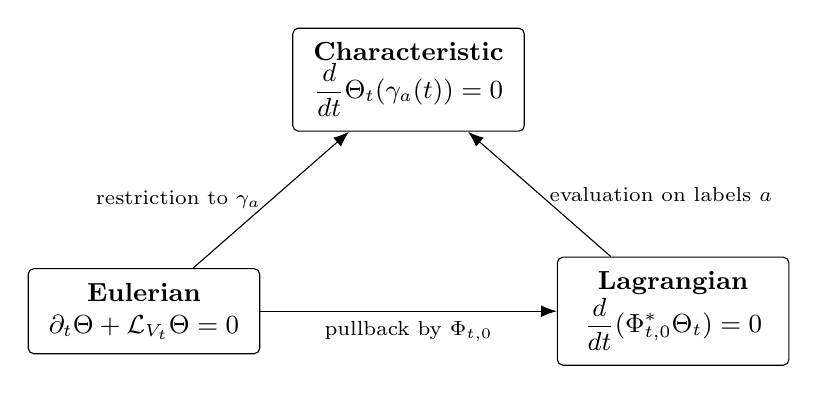
\begin{tikzpicture}[node distance=3.2cm, scale=1.05, every node/.style={scale=1.05}]
  \node[ccbox, align=center, minimum width=2.8cm] (E) at (-3.2,0) {\textbf{Eulerian}\\$\partial_t \Theta + \mathcal L_{V_t}\Theta = 0$};
  \node[ccbox, align=center, minimum width=2.8cm] (L) at (3.2,0) {\textbf{Lagrangian}\\$\dfrac{d}{dt}(\Phi_{t,0}^*\Theta_t)=0$};
  \node[ccbox, align=center, minimum width=2.8cm] (C) at (0,2.8) {\textbf{Characteristic}\\$\dfrac{d}{dt}\Theta_t(\gamma_a(t))=0$};

  \draw[ccarrow] (E) -- node[below, cclabel] {pullback by $\Phi_{t,0}$} (L);
  \draw[ccarrow] (E) -- node[left, cclabel] {restriction to $\gamma_a$} (C);
  \draw[ccarrow] (L) -- node[right, cclabel] {evaluation on labels $a$} (C);
\end{tikzpicture}
\caption{Observer-side compatibility of the Eulerian, Lagrangian, and characteristic presentations of a conservative transport law.}
\label{fig:observer-triad}
\end{figure}

\begin{proposition}[Observer-Side Compatibility]
\label{prop:observer-triad}
\lean{observer_triad}
Under the standing hypotheses above, Definitions~\ref{def:eulerian-presentation},
\ref{def:lagrangian-presentation}, and
\ref{def:characteristic-presentation} are equivalent.
\end{proposition}

(Proof in Appendix~\ref{sec:appendix-dynamics}.)

\begin{definition}[Characteristic Flux Form]
\label{def:characteristic-flux-form}
\lean{CharacteristicFluxForm}
For a transported scalar $\Theta$ on $X$, define the \emph{characteristic flux
form}
\[
J_\Theta := \Theta \,\iota_{\widetilde V}\nu.
\]
\end{definition}

\begin{lemma}[Flux Differential Identity]
\label{lem:flux-differential}
\lean{flux_differential}
With notation as above,
\[
dJ_\Theta = (\mathcal D_\chi \Theta)\,\nu.
\]
\end{lemma}

(Proof in Appendix~\ref{sec:appendix-dynamics}.)

\begin{theorem}[Cut Conservation]
\label{thm:cut-conservation}
\lean{cut_conservation}
Let $U \subset X$ be a compact spacetime tube whose boundary decomposes as
\[
\partial U = \Sigma_1 - \Sigma_0 + \Sigma_{\mathrm{side}},
\]
where $\Sigma_0$ and $\Sigma_1$ are transverse cuts and
$\widetilde V$ is tangent to the side boundary
$\Sigma_{\mathrm{side}}$. If $\mathcal D_\chi \Theta = 0$ on $U$, then
\[
\int_{\Sigma_1} J_\Theta = \int_{\Sigma_0} J_\Theta.
\]
\end{theorem}

(Proof in Appendix~\ref{sec:appendix-dynamics}.)

\begin{theorem}[Characteristic Integration by Parts]
\label{thm:characteristic-ibp}
\lean{characteristic_ibp}
Let $f,g \in C^\infty(U)$ on a compact spacetime tube $U \subset X$. Then
\[
\int_U \bigl((\mathcal D_\chi f)g + f(\mathcal D_\chi g)\bigr)\,\nu
=
\int_{\partial U} fg\,\iota_{\widetilde V}\nu.
\]
\end{theorem}

(Proof in Appendix~\ref{sec:appendix-dynamics}.)

\begin{corollary}[Characteristic Boundary Reduction]
\label{cor:characteristic-boundary-reduction}
\lean{characteristic_boundary_reduction}
If $\mathcal D_\chi f = 0$ on $U$, then
\[
\int_U f(\mathcal D_\chi g)\,\nu
=
\int_{\partial U} fg\,\iota_{\widetilde V}\nu.
\]
Thus conservative transport along characteristic directions removes the bulk
term and leaves only the boundary contribution.
\end{corollary}

\begin{proof}
Substitute $\mathcal D_\chi f = 0$ into
Theorem~\ref{thm:characteristic-ibp}.
\end{proof}

The same elimination mechanism has a direct cellular formulation closer to the
finite observer setting of the structural calculus.

\begin{definition}[Cellular Conservative Current]
\label{def:cellular-current}
\lean{CellularConservativeCurrent}
Let $K$ be a locally finite oriented cell complex. A cochain
$J \in C^1(K;\bbR)$ is called a \emph{cellular conservative current} on a finite
$2$-chain $C$ if
\[
\langle \delta J,\sigma\rangle = 0
\]
for every $2$-cell $\sigma$ in the support of $C$.
\end{definition}

\begin{proposition}[Cellular Cut Conservation]
\label{prop:cellular-cut-conservation}
\lean{cellular_cut_conservation}
Let $\Gamma_0,\Gamma_1$ be finite $1$-cycles in $K$ such that
\[
\Gamma_1-\Gamma_0=\partial C
\]
for some finite $2$-chain $C$. If $J$ is a cellular conservative current on
$C$, then
\[
\langle J,\Gamma_1\rangle = \langle J,\Gamma_0\rangle.
\]
\end{proposition}

(Proof in Appendix~\ref{sec:appendix-dynamics}.)

Proposition~\ref{prop:cellular-cut-conservation} is the discrete companion of
Theorem~\ref{thm:cut-conservation}: in both regularity classes, conservative
transport reduces finite observation to boundary data on cuts.

\subsection{Horizon Realization of the Calculus}

Characteristic transport supplies the boundary law. To recover the operator
calculus of Part~I, the full state space must also carry a closed differential
together with a finite horizon decomposition.

\begin{definition}[Characteristic Horizon Realization]
\label{def:characteristic-horizon-realization}
\lean{CharacteristicHorizonRealization}
A \emph{characteristic horizon realization} consists of the following data.
\begin{enumerate}[label=(\roman*), leftmargin=2em, itemsep=0.2em]
\item A Hilbert complex $(\cH^\bullet,d)$ with $d^2=0$.
\item A nested family of orthogonal projections
      $\{\CCPi{h}\}_{h \in \bbN}$ on each degree of $\cH^\bullet$.
\item A strongly continuous unitary transport family $\{U_t\}_{t \in J}$ on
      $\cH^\bullet$ such that
      \[
      U_t d = d U_t,
      \qquad
      U_t \CCPi{h} = \CCPi{h} U_t
      \quad \text{for all } h \in \bbN.
      \]
\end{enumerate}
The realized observed operator, leakage operator, and defect operator are
defined exactly as in Part~I:
\[
\CCObs{d}{h} = \CCPi{h} d \CCPi{h},
\qquad
\CCLeak{d}{h} = \CCPibar{h} d \CCPi{h},
\qquad
\CCDefect{d}{h} = \CCPi{h} d \CCPibar{h} d \CCPi{h}.
\]
\end{definition}

\begin{figure}[ht]
\centering
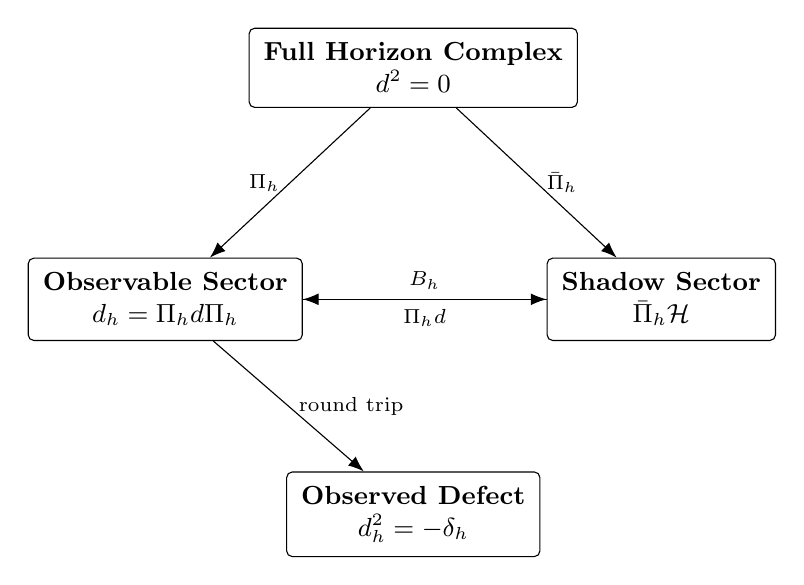
\begin{tikzpicture}[node distance=2.8cm, scale=1.05, every node/.style={scale=1.05}]
  \node[ccbox, align=center, minimum width=2.6cm] (bulk) at (0,2.8) {\textbf{Full Horizon Complex}\\$d^2 = 0$};
  \node[ccbox, align=center, minimum width=2.6cm] (obs) at (-3,0) {\textbf{Observable Sector}\\$\CCObs{d}{h}=\CCPi{h} d \CCPi{h}$};
  \node[ccbox, align=center, minimum width=2.6cm] (sh) at (3,0) {\textbf{Shadow Sector}\\$\CCPibar{h}\cH$};
  \node[ccbox, align=center, minimum width=3.0cm] (def) at (0,-2.6) {\textbf{Observed Defect}\\$\CCObs{d}{h}^2 = -\CCDefect{d}{h}$};

  \draw[ccarrow] (bulk) -- node[left, cclabel] {$\CCPi{h}$} (obs);
  \draw[ccarrow] (bulk) -- node[right, cclabel] {$\CCPibar{h}$} (sh);
  \draw[ccarrow] (obs) -- node[above, cclabel] {$\CCLeak{d}{h}$} (sh);
  \draw[ccarrow] (sh) -- node[below, cclabel] {$\CCPi{h} d$} (obs);
  \draw[ccarrow] (obs) -- node[right, cclabel] {round trip} (def);
\end{tikzpicture}
\caption{Full closure holds on the horizon complex. Finite observation inserts a horizon cut, and the observed failure of closure is exactly the round trip through shadow.}
\label{fig:bulk-to-defect}
\end{figure}

\begin{lemma}[Through-Horizon Decomposition]
\label{lem:through-horizon-decomposition}
\lean{through_horizon_decomposition}
For every observed state $u \in \CCPi{h}\cH^\bullet$,
\[
du = \CCObs{d}{h}u + \CCLeak{d}{h}u.
\]
Applying $d$ once more and projecting back to the observed sector gives
\[
\CCPi{h}d\,\CCObs{d}{h}u = -\,\CCPi{h}d\,\CCLeak{d}{h}u = -\,\CCDefect{d}{h}u.
\]
\end{lemma}

(Proof in Appendix~\ref{sec:appendix-dynamics}.)

\begin{theorem}[Characteristic Realization of HFT]
\label{thm:characteristic-realization}
\lean{characteristic_realization}
Let $(\cH^\bullet,d,\{\CCPi{h}\},\{U_t\})$ be a characteristic horizon
realization. Then, for every horizon $h$,
\[
\CCObs{d}{h}^2 = - \CCDefect{d}{h}.
\]
Moreover,
\[
U_t \CCObs{d}{h} = \CCObs{d}{h} U_t,
\qquad
U_t \CCDefect{d}{h} = \CCDefect{d}{h} U_t,
\]
so the realized observed differential and its defect are transported
equivariantly by the conservative evolution.
\end{theorem}

(Proof in Appendix~\ref{sec:appendix-dynamics}.)

\begin{theorem}[Characteristic horizon realizations transport the horizon complex]
\label{thm:characteristic-horizon-realizations-transport-the-horizon-complex}\lean{CharacteristicHorizonRealization.horizonComplex}\lean{CharacteristicHorizonRealization.horizonComplexSurface}
Every characteristic horizon realization carries the Part~I horizon-complex
laws unchanged. Concretely, on the same realized carrier:
\begin{enumerate}[label=(\roman*), leftmargin=2em, itemsep=0.2em]
\item the full boundary still satisfies \(d^2=0\);
\item on every cut, the observed boundary still satisfies
      \(\CCObs{d}{h}^2=-\,\CCDefect{d}{h}\);
\item the conservative transport intertwines both the observed boundary and the
      defect:
      \[
      U_t\CCObs{d}{h}=\CCObs{d}{h}U_t,
      \qquad
      U_t\CCDefect{d}{h}=\CCDefect{d}{h}U_t.
      \]
\end{enumerate}
So a characteristic horizon realization is best understood as a transport
realization of a horizon complex, not merely as an external flow laid on top of
the Part~I state space.
\end{theorem}

\begin{proof}
The associated horizon complex uses the same tower and the same full boundary
\(d\). The closure and cut-defect clauses are exactly the transported Part~I
laws, and the transport identities are the content of
Theorem~\ref{thm:characteristic-realization}.
\end{proof}

\begin{corollary}[Transfer to the Part~I Calculus]
\label{cor:transfer-part-one}
\lean{transfer_part_one}
Every statement of Part~I whose hypotheses involve only the closed operator
$d$, the horizon tower $\{\CCPi{h}\}$, and the algebra they generate applies to
every characteristic horizon realization.
\end{corollary}

\begin{proof}
By Definition~\ref{def:characteristic-horizon-realization}, the realized data
has exactly the same formal type as the operator interface of Part~I. By
Theorem~\ref{thm:characteristic-realization}, the realized observed operator
satisfies the Horizon Fundamental Theorem with the same proof as in the abstract
setting. Any further theorem in Part~I that depends only on that interface
therefore transports unchanged to the realized class.
\end{proof}

\subsection{Variational Realization and the Dynamics-Side Triad}

The observer-side triad concerns the transport of conserved quantities along a
given characteristic field. A different question concerns the origin of that
field when the dynamics are generated by an action principle. The corresponding
classical triad is Lagrangian, Hamiltonian, and characteristic. Here the
Hamiltonian formulation is the phase-space evolution law, whereas the
characteristic formulation refers to the characteristic curves of the
Hamilton--Jacobi equation. The distinguished trajectories are the stationary
action curves seen simultaneously in both languages
\cite{Arnold1989}.

\begin{definition}[Regular Variational System]
\label{def:regular-variational-system}
\lean{RegularVariationalSystem}
Let $Q$ be a smooth configuration manifold and let
$L \in C^2(TQ \times J)$ be a Lagrangian whose fiber Hessian in the velocity
variables is everywhere invertible. The Legendre transform
\[
\mathbb F L : TQ \to T^*Q,
\qquad
(q,\dot q) \mapsto \Bigl(q,\frac{\partial L}{\partial \dot q}\Bigr)
\]
then defines a local diffeomorphism and determines the Hamiltonian
$H \in C^2(T^*Q \times J)$ by
\[
H(q,p,t) = p\cdot \dot q - L(q,\dot q,t),
\]
with $\dot q$ understood as the inverse Legendre image of $(q,p)$.
\end{definition}

\begin{figure}[ht]
\centering
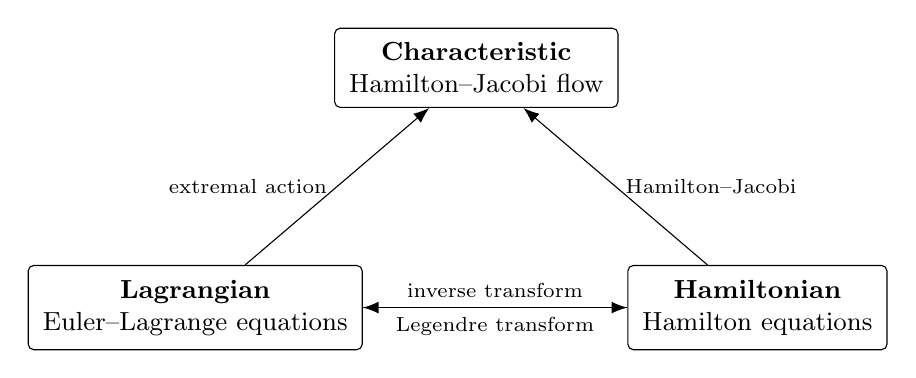
\begin{tikzpicture}[node distance=3.4cm, scale=1.05, every node/.style={scale=1.05}]
  \node[ccbox, align=center, minimum width=2.9cm] (C) at (0,2.9) {\textbf{Characteristic}\\Hamilton--Jacobi flow};
  \node[ccbox, align=center, minimum width=2.9cm] (L) at (-3.4,0) {\textbf{Lagrangian}\\Euler--Lagrange equations};
  \node[ccbox, align=center, minimum width=2.9cm] (H) at (3.4,0) {\textbf{Hamiltonian}\\Hamilton equations};

  \draw[ccarrow] (L) -- node[below, cclabel] {Legendre transform} (H);
  \draw[ccarrow] (H) -- node[above, cclabel] {inverse transform} (L);
  \draw[ccarrow] (L) -- node[left, cclabel] {extremal action} (C);
  \draw[ccarrow] (H) -- node[right, cclabel] {Hamilton--Jacobi} (C);
\end{tikzpicture}
\caption{Dynamics-side compatibility of the Lagrangian, Hamiltonian, and characteristic presentations for a regular variational system.}
\label{fig:dynamics-triad}
\end{figure}

\begin{theorem}[Dynamics-Side Triad Equivalence]
\label{thm:dynamics-triad}
\lean{dynamics_triad}
Let $L$ be a regular variational system in the sense of
Definition~\ref{def:regular-variational-system}, let $H$ be its Hamiltonian,
and let $S \in C^2(Q \times J)$ satisfy the Hamilton--Jacobi equation
\[
\partial_t S(q,t) + H\bigl(q,\partial_q S(q,t),t\bigr)=0
\]
on a simply connected domain. Then the following descriptions determine the same
local trajectories:
\begin{enumerate}[label=(\roman*), leftmargin=2em, itemsep=0.2em]
\item stationary curves of the action $\int L(q,\dot q,t)\,dt$;
\item solutions of Hamilton's equations for $H$;
\item characteristic curves of the Hamilton--Jacobi equation, given by
      \[
      p=\partial_q S,
      \qquad
      \dot q = \partial_p H(q,p,t).
      \]
\end{enumerate}
\end{theorem}

(Proof in Appendix~\ref{sec:appendix-dynamics}.)

\begin{proposition}[Characteristic Projection of Hamilton--Jacobi Dynamics]
\label{prop:hj-projection}
\lean{hj_projection}
Let $S$ satisfy the hypotheses of
Theorem~\ref{thm:dynamics-triad}, and define the time-dependent vector field
\[
V_t(q) := \partial_p H\bigl(q,\partial_q S(q,t),t\bigr)
\]
on $Q$. Then the integral curves of $V_t$ are exactly the configuration-space
projections of the Hamiltonian trajectories lying in the Lagrangian graph
\[
\Gamma_t := \{(q,\partial_q S(q,t)) : q \in Q\} \subset T^*Q.
\]
Consequently, the observer-side characteristic curves generated by
$\mathcal D_\chi = \partial_t + \mathcal L_{V_t}$ are precisely the projected
dynamics-side characteristics of the Hamilton--Jacobi equation.
\end{proposition}

(Proof in Appendix~\ref{sec:appendix-dynamics}.)

\begin{proposition}[Selection Principle for Realized Classes]
\label{prop:selection-problem}
\lean{selection_problem}
Let $\mathfrak R$ be any class of characteristic horizon realizations that also
arises from regular variational systems satisfying
Theorem~\ref{thm:dynamics-triad}. Then the existence of the Part~I calculus is
uniform on $\mathfrak R$. Any theorem asserting a unique admissible horizon, a
distinguished completion, or a canonical dimensionless invariant on
$\mathfrak R$ must therefore enter through additional \emph{selection
hypotheses} on the realized class rather than through realization alone.
\end{proposition}

(Proof in Appendix~\ref{sec:appendix-dynamics}.)

\subsection{From Realization to Forcing}

Proposition~\ref{prop:selection-problem} identifies the point at which
uniqueness may enter. The next definitions isolate the corresponding selection
data and admissible realized classes. The resulting theorem is constructive:
once a realized class has been specified, the remaining forcing problem is an
explicit admissibility problem on reduced operator data.

\begin{definition}[Selection datum at a fixed horizon]
\label{def:selection-datum}
\lean{SelectionDatum}
Fix a horizon $h$ and let
\[
R=(\cH^\bullet,d,\{\CCPi{k}\}_{k\in\bbN},\{U_t\}_{t\in J})
\]
be a characteristic horizon realization. A \emph{selection datum} for $R$ at
horizon $h$ consists of:
\begin{enumerate}[label=(\roman*), leftmargin=2em, itemsep=0.2em]
\item the observed sector $\CCHobs{h}(R):=\CCPi{h}\cH^\bullet$ together with the
      realized observed differential $\CCObs{d}{h}$ and defect
      $\CCDefect{d}{h}$;
\item a self-adjoint lower-bound operator $D_h$ on $\CCHobs{h}(R)$ derived from
      defect propagation and, when present, elimination/residual terms on the
      observed sector;
\item a finite-dimensional family $\mathcal Q_h(R)$ of candidate self-adjoint
      reduced laws or completion data on $\CCHobs{h}(R)$;
\item a unitary action of a finite group $G_h$ on $\CCHobs{h}(R)$ preserving
      $D_h$ and $\mathcal Q_h(R)$;
\item a family $\mathcal N_h$ of normalization, compatibility, or scale-fixing
      conditions imposed on $\mathcal Q_h(R)$.
\end{enumerate}
Such a datum will be denoted by $\mathsf S_h(R)$.
Locality and horizon compatibility are encoded in the choice of the
finite-dimensional candidate family $\mathcal Q_h(R)$ inside the realized
class.
\end{definition}

\begin{definition}[Horizon-preserving equivalence]
\label{def:horizon-preserving-equivalence}
\lean{HorizonPreservingEquivalence}
Two selection data
\[
\mathsf S_h(R)
\qquad\text{and}\qquad
\mathsf S_h(R')
\]
at the same horizon are \emph{horizon-preserving equivalent} if there exists a
unitary isomorphism
\[
W:\CCHobs{h}(R)\to \CCHobs{h}(R')
\]
such that:
\begin{enumerate}[label=(\roman*), leftmargin=2em, itemsep=0.2em]
\item $W\,\CCObs{d}{h} = \CCObs{d'}{h}\,W$ and
      $W\,\CCDefect{d}{h} = \CCDefect{d'}{h}\,W$;
\item $W D_h = D_h' W$;
\item $W\,\mathcal Q_h(R)\,W^{-1} = \mathcal Q_h(R')$;
\item $W$ intertwines the $G_h$-actions and preserves the normalization data
      $\mathcal N_h$.
\end{enumerate}
Equivalent selection data represent the same reduced observed law in different
coordinates.
\end{definition}

\begin{definition}[Admissible realized class]
\label{def:admissible-realized-class}
\lean{AdmissibleRealizedClass}
Fix a horizon $h$. An \emph{admissible realized class} at horizon $h$ is a
subclass $\mathfrak R_{\mathrm{adm}}(h)\subseteq \mathfrak R$ consisting of
those characteristic horizon realizations that are equipped with a selection
datum satisfying the following requirements:
\begin{enumerate}[label=(\roman*), leftmargin=2em, itemsep=0.2em]
\item the candidate family $\mathcal Q_h(R)$ is finite-dimensional;
\item the admissibility constraint of
      Definition~\ref{def:admissibility} is well posed for the derived
      lower-bound operator $D_h$ on $\CCHobs{h}(R)$;
\item $D_h$ and $\mathcal Q_h(R)$ are $G_h$-equivariant;
\item the normalization data $\mathcal N_h$ are invariant under
      horizon-preserving equivalence.
\end{enumerate}
If the horizon itself is part of the selection problem, one may further attach
a design objective on an appropriate Grassmannian as in
Definition~\ref{def:design-objective}.
\end{definition}

\begin{theorem}[Constructive Selection Interface for Realized Classes]
\label{thm:selection-interface}
\lean{selection_interface}
Fix a horizon $h$ and an admissible realized class
$\mathfrak R_{\mathrm{adm}}(h)$. Then for every
$R\in\mathfrak R_{\mathrm{adm}}(h)$ the forcing problem on the realized class
reduces to a finite and checkable selection problem:
\begin{enumerate}[label=(\roman*), leftmargin=2em, itemsep=0.2em]
\item the structural calculus of Part~I applies to $R$ on
      $\CCHobs{h}(R)$;
\item after symmetry reduction, the admissible reduced operator data are
      parameterized by finitely many block variables on the multiplicity spaces
      of the $G_h$-isotypic decomposition;
\item the completion-and-selection algebra of Chapter~5 returns exactly one of the following outputs:
      a unique admissible reduced datum, a minimal residual face
      certifying non-uniqueness, or an inconsistency certificate;
\item if horizon selection is included through a Grassmannian design objective,
      then optimal horizons exist in finite dimensions and satisfy the
      stationary commutator equation
      \[
      [\nabla \CCDesign{P^\star},P^\star]=0.
      \]
\end{enumerate}
In particular, realization plus admissibility converts the forcing question
into an explicit reduced problem on finite-dimensional operator data.
\end{theorem}

(Proof in Appendix~\ref{sec:appendix-dynamics}.)

\begin{definition}[Selected observed law]
\label{def:selected-observed-law}
\lean{selected_observed_law}
Let $R\in\mathfrak R_{\mathrm{adm}}(h)$. If the admissibility output in
Theorem~\ref{thm:selection-interface}(iii) is unique, and if any horizon
optimization included in the datum also yields a unique horizon up to
horizon-preserving equivalence, then the resulting reduced operator datum is
called the \emph{selected observed law} of $R$ at horizon $h$.
\end{definition}

\begin{corollary}[Selection-to-Forcing Principle]
\label{cor:selection-to-forcing}
\lean{selection_to_forcing}
Fix a horizon $h$ and an admissible realized class
$\mathfrak R_{\mathrm{adm}}(h)$. Suppose the admissible reduced selection data
modulo horizon-preserving equivalence consist of a single equivalence class.
Then the selected observed law is forced on
$\mathfrak R_{\mathrm{adm}}(h)$: every realization in
$\mathfrak R_{\mathrm{adm}}(h)$ yields the same selected observed law up to
horizon-preserving equivalence.
\end{corollary}

\begin{proof}
By Theorem~\ref{thm:selection-interface}, each realization in
$\mathfrak R_{\mathrm{adm}}(h)$ reduces to a finite admissibility problem on
its reduced operator data. By hypothesis, the admissible reduced data modulo
horizon-preserving equivalence form a singleton. Therefore the unique
selection output of Definition~\ref{def:selected-observed-law} is the same for
every realization up to that equivalence. Hence the observed law is forced on
the class, modulo change of coordinates preserving horizons, symmetry, and
normalization.
\end{proof}

\begin{definition}[Intrinsically equivariant realized class]\lean{IntrinsicallyEquivariantRealizedClass}
\label{def:intrinsically-equivariant-realized-class}
Fix a horizon $h$. An admissible realized class
$\mathfrak R_{\mathrm{adm}}(h)$ is \emph{intrinsically equivariant on the
canonical carrier} if each realization
$R\in\mathfrak R_{\mathrm{adm}}(h)$ is equipped with a unitary identification
\[
W_R:\CCHobs{h}(R)\to V_{\mathrm{slot}}
\]
onto the canonical six-slot carrier of
Definition~\ref{def:local-slot-carrier} such that:
\begin{enumerate}[label=(\roman*), leftmargin=2em, itemsep=0.2em]
\item the transported symmetry group $G_h$ is the intrinsic relabeling action
      of $S_4$ on $V_{\mathrm{slot}}$ from
      Definition~\ref{def:intrinsic-relabeling-action};
\item the transported lower-bound operator and candidate family are
      $S_4$-equivariant on $V_{\mathrm{slot}}$;
\item the normalization data are invariant under the same $S_4$ action.
\end{enumerate}
\end{definition}

\begin{theorem}[Intrinsic-equivariant forcing on the canonical carrier]\lean{intrinsic_equivariant_forcing}
\label{thm:intrinsic-equivariant-forcing}
Fix a horizon $h$ and let $\mathfrak R_{\mathrm{adm}}(h)$ be an intrinsically
equivariant realized class on the canonical carrier. Suppose the admissible
reduced selection data modulo horizon-preserving equivalence consist of a
single equivalence class. Then there exist unique scalars $a,b,c\in\bbR$ such
that for every $R\in\mathfrak R_{\mathrm{adm}}(h)$, the selected observed law
$L_R$ of $R$ satisfies
\[
W_R L_R W_R^{-1} e_\alpha
=
a\,e_\alpha
+
b\sum_{\beta\sim\alpha}e_\beta
+
c\sum_{\beta\perp\alpha}e_\beta
\qquad(\alpha\in\mathcal S_4).
\]
Equivalently, after transport to the canonical carrier, the selected observed
law is the same intrinsic-equivariant three-parameter operator for every
realization in the class. Its channel eigenvalues on the forced $1+2+3$
decomposition are
\[
\lambda_1=a+4b+c,\qquad
\lambda_2=a-2b+c,\qquad
\lambda_3=a-c.
\]
\end{theorem}

(Proof in Appendix~\ref{sec:appendix-dynamics}.)

\begin{definition}[Subgroup-broken realized class]\lean{SubgroupBrokenRealizedClass}
\label{def:subgroup-broken-realized-class}
Let $H\le S_4$ be a subgroup. An admissible realized class
$\mathfrak R_{\mathrm{adm}}(h)$ is \emph{$H$-equivariant on the canonical
carrier} if each realization admits a unitary identification
\[
W_R:\CCHobs{h}(R)\to V_{\mathrm{slot}}
\]
for which the transported symmetry, lower-bound operator, candidate family, and
normalization data are all invariant under the restricted action of $H$ on
$V_{\mathrm{slot}}$.
\end{definition}

\begin{proposition}[Finite subgroup-broken selection]\lean{finite_subgroup_broken_selection}
\label{prop:finite-subgroup-broken-selection}
Let $H\le S_4$ and let $\mathfrak R_{\mathrm{adm}}(h)$ be an
$H$-equivariant realized class on the canonical carrier. Then any selected
observed law on $\mathfrak R_{\mathrm{adm}}(h)$ decomposes blockwise on the
$H$-isotypic decomposition of $V_{\mathrm{slot}}$. In particular:
\begin{enumerate}[label=(\roman*), leftmargin=2em, itemsep=0.2em]
\item the corresponding reduced channel problem is still finite-dimensional;
\item the number of irreducible local channels is at most $6$;
\item the full intrinsic-equivariant case $H=S_4$ recovers the forced
      three-parameter $1+2+3$ law of
      Theorem~\ref{thm:intrinsic-equivariant-forcing}.
\end{enumerate}
\end{proposition}

\begin{proof}
After transport by $W_R$, the selected law is $H$-equivariant on the
six-dimensional carrier $V_{\mathrm{slot}}$. Theorem~\ref{thm:normal-form} and
Corollary~\ref{cor:isotypic-block} therefore reduce the law to block variables
on the multiplicity spaces of the $H$-isotypic decomposition. Because
$V_{\mathrm{slot}}$ has dimension $6$, there can be at most six nonzero
irreducible channels. This proves (i) and (ii). Statement (iii) is exactly the
special case $H=S_4$, where
Theorem~\ref{thm:intrinsic-equivariant-forcing} applies.
\end{proof}

\begin{definition}[Complex-type realized class]\lean{ComplexTypeRealizedClass}
\label{def:complex-type-realized-class}
Fix a horizon $h$. An admissible realized class
$\mathfrak R_{\mathrm{adm}}(h)$ is \emph{complex-type with scalar multiplicity
commutant} if, for every realization $R\in\mathfrak R_{\mathrm{adm}}(h)$:
\begin{enumerate}[label=(\roman*), leftmargin=2em, itemsep=0.2em]
\item the observed sector $\CCHobs{h}(R)$ carries a finite unitary symmetry
      action and an isotypic decomposition on the relevant selected-law sector;
\item the transported selected observed law and admissible selection data are
      equivariant for that action;
\item the selected-law sector carries a complex-type multiplicity package in
      the sense of Definition~\ref{def:complex-type-multiplicity-package};
\item on each isotypic channel, the induced multiplicity-space action of the
      selected-law family has scalar multiplicity commutant in the sense of
      Definition~\ref{def:scalar-multiplicity-commutant}.
\end{enumerate}
\end{definition}

\begin{corollary}[Realized phase-carrier class forcing]\lean{realized_phase_class_forcing}
\label{cor:realized-phase-class-forcing}
Fix a horizon $h$ and let $\mathfrak R_{\mathrm{adm}}(h)$ be a complex-type
realized class with scalar multiplicity commutant. Suppose the admissible
reduced selection data modulo horizon-preserving equivalence consist of a
single equivalence class. Then the selected law on
$\mathfrak R_{\mathrm{adm}}(h)$ carries a forced phase-carrier class modulo
phase-equivalence.
\end{corollary}

(Proof in Appendix~\ref{sec:appendix-dynamics}.)

\begin{definition}[Observable-irreducible realized class]\lean{ObservableIrreducibleRealizedClass}
\label{def:observable-irreducible-realized-class}
Fix a horizon $h$. An admissible realized class
$\mathfrak R_{\mathrm{adm}}(h)$ is \emph{observable-irreducible on the selected
channels} if, for every realization $R\in\mathfrak R_{\mathrm{adm}}(h)$ and
for every isotypic channel appearing in the selected-law sector:
\begin{enumerate}[label=(\roman*), leftmargin=2em, itemsep=0.2em]
\item the selected-law family acts on the corresponding multiplicity space
      through a family $\mathcal A_{\rho}(R)$ as in
      Definition~\ref{def:observable-irreducibility};
\item the family $\mathcal A_{\rho}(R)$ is observable-irreducible;
\item every selected self-adjoint closure or quadratic transport operator on
      that channel commutes with $\mathcal A_{\rho}(R)$.
\end{enumerate}
\end{definition}

\begin{corollary}[Realized self-adjoint scalarization on observable-irreducible channels]\lean{realized_self_adjoint_scalarization}
\label{cor:realized-self-adjoint-scalarization}
Fix a horizon $h$ and let $\mathfrak R_{\mathrm{adm}}(h)$ be an
observable-irreducible realized class. Then every selected self-adjoint
closure or quadratic transport operator on a selected channel is scalar on the
corresponding multiplicity space.
\end{corollary}

\begin{proof}
By Definition~\ref{def:observable-irreducible-realized-class}, the selected
self-adjoint operator on each channel commutes with an observable-irreducible
family on the corresponding multiplicity space. Corollary~\ref{cor:self-adjoint-commutant-scalarization}
then forces that operator to be a real scalar multiple of the identity on that
multiplicity space.
\end{proof}

\begin{corollary}[Realized isotropic symmetric-response scalarization]\lean{realized_isotropic_symmetric_response_scalarization}
\label{cor:realized-isotropic-symmetric-response-scalarization}
Fix a horizon $h$ and let $\mathfrak R_{\mathrm{adm}}(h)$ be an admissible
realized class. Assume that on a selected channel fiber the observable carrier
is the symmetric-tensor carrier $\mathrm{Sym}^2(F_h)$ of a real
$d$-dimensional inner-product space $F_h$ with $d\ge 2$, and that the selected
leading response operator
\[
\mathcal L_h:\mathrm{Sym}^2(F_h)\to \mathrm{Sym}^2(F_h)
\]
is equivariant for the induced orthogonal conjugation action of $O(F_h)$.
Then there are unique scalars $\alpha_h,\beta_h\in\bbR$ such that
\[
\mathcal L_h(S)
=
\alpha_h\Bigl(S-\frac{\operatorname{tr}(S)}{d}I\Bigr)
+
\beta_h\,\frac{\operatorname{tr}(S)}{d}I
\qquad\text{for every }S\in \mathrm{Sym}^2(F_h).
\]
In particular, the trace line $\bbR I$ and the traceless carrier
$\mathrm{Sym}^2_0(F_h)$ are the intrinsic scalar channels of the selected
response.
\end{corollary}

\begin{proof}
Choose an orthonormal identification $F_h\cong \bbR^d$. Under that
identification, the induced orthogonal conjugation action on
$\mathrm{Sym}^2(F_h)$ becomes the standard $O(d)$-action on
$\mathrm{Sym}^2(\bbR^d)$, and $\mathcal L_h$ satisfies the hypotheses of
Theorem~\ref{thm:orthogonal-symmetric-tensor-scalarization}. The resulting
scalars are independent of the chosen orthonormal identification because the
formula in that theorem is itself orthogonally invariant.
\end{proof}

\begin{corollary}[Realized phase forcing from real-type observable irreducibility]\lean{realized_phase_from_real_type}
\label{cor:realized-phase-from-real-type}
Fix a horizon $h$ and let $\mathfrak R_{\mathrm{adm}}(h)$ be an admissible
realized class such that:
\begin{enumerate}[label=(\roman*), leftmargin=2em, itemsep=0.2em]
\item on each relevant selected-law channel, the observed sector carries the
      data of a complex-type multiplicity package in the sense of
      Definition~\ref{def:complex-type-multiplicity-package};
\item on each relevant multiplicity space, the selected-law family is
      observable-irreducible and of real type in the sense of
      Definitions~\ref{def:observable-irreducibility} and
      \ref{def:real-type-observable-channel};
\item the admissible reduced selection data modulo horizon-preserving
      equivalence consist of a single equivalence class.
\end{enumerate}
Then the selected law on $\mathfrak R_{\mathrm{adm}}(h)$ carries a forced
phase-carrier class modulo phase-equivalence.
\end{corollary}

\begin{proof}
By Corollary~\ref{cor:selection-to-forcing}, the selected observed law is
forced on $\mathfrak R_{\mathrm{adm}}(h)$ up to horizon-preserving
equivalence. On each channel, the real-type observable irreducibility
hypothesis lets
Corollary~\ref{cor:real-type-irreducibility-collapses-phase-gauge} collapse
the residual phase gauge to a unique class modulo phase-equivalence. These
channelwise phase classes therefore agree across the realized class up to the
same equivalence.
\end{proof}

\begin{corollary}[Realized phase forcing from adjoint-closed real type]\lean{realized_phase_from_adjoint_closed_real_type}
\label{cor:realized-phase-from-adjoint-closed-real-type}
Fix a horizon $h$ and let $\mathfrak R_{\mathrm{adm}}(h)$ be an admissible
realized class such that:
\begin{enumerate}[label=(\roman*), leftmargin=2em, itemsep=0.2em]
\item on each relevant selected-law channel, the observed sector carries the
      data of a complex-type multiplicity package in the sense of
      Definition~\ref{def:complex-type-multiplicity-package};
\item on each relevant multiplicity space, the selected-law family is
      observable-irreducible, of real type, and adjoint-closed in generation
      in the sense of Definitions~\ref{def:observable-irreducibility},
      \ref{def:real-type-observable-channel}, and
      \ref{def:adjoint-closed-generated-observable-algebra};
\item the admissible reduced selection data modulo horizon-preserving
      equivalence consist of a single equivalence class.
\end{enumerate}
Then the selected law on $\mathfrak R_{\mathrm{adm}}(h)$ carries a forced
phase-carrier class modulo phase-equivalence.
\end{corollary}

\begin{proof}
By Corollary~\ref{cor:selection-to-forcing}, the selected observed law is
forced on $\mathfrak R_{\mathrm{adm}}(h)$ up to horizon-preserving
equivalence. On each channel, the adjoint-closed real-type hypothesis lets
Corollary~\ref{cor:adjoint-closed-real-type-phase} collapse the residual phase
gauge to a unique class modulo phase-equivalence. These channelwise phase
classes therefore agree across the realized class up to the same equivalence.
\end{proof}

\begin{corollary}[Realized phase forcing from a rank-one observable seed]\lean{realized_phase_from_rank_one_seed}
\label{cor:realized-phase-from-rank-one-seed}
Fix a horizon $h$ and let $\mathfrak R_{\mathrm{adm}}(h)$ be an admissible
realized class such that:
\begin{enumerate}[label=(\roman*), leftmargin=2em, itemsep=0.2em]
\item on each relevant selected-law channel, the observed sector carries the
      data of a complex-type multiplicity package in the sense of
      Definition~\ref{def:complex-type-multiplicity-package};
\item on each relevant multiplicity space, the selected-law family is
      observable-irreducible, adjoint-closed in generation, and carries a
      rank-one observable seed in the sense of
      Definitions~\ref{def:observable-irreducibility},
      \ref{def:adjoint-closed-generated-observable-algebra}, and
      \ref{def:rank-one-observable-seed};
\item the admissible reduced selection data modulo horizon-preserving
      equivalence consist of a single equivalence class.
\end{enumerate}
Then the selected law on $\mathfrak R_{\mathrm{adm}}(h)$ carries a forced
phase-carrier class modulo phase-equivalence.
\end{corollary}

\begin{proof}
By Corollary~\ref{cor:selection-to-forcing}, the selected observed law is
forced on $\mathfrak R_{\mathrm{adm}}(h)$ up to horizon-preserving
equivalence. On each channel, the rank-one seed hypothesis lets
Corollary~\ref{cor:rank-one-seed-phase} collapse the residual phase gauge to a
unique class modulo phase-equivalence. These channelwise phase classes
therefore agree across the realized class up to the same equivalence.
\end{proof}

\begin{corollary}[Realized phase forcing from simple spectrum]\lean{realized_phase_from_simple_spectrum}
\label{cor:realized-phase-from-simple-spectrum}
Fix a horizon $h$ and let $\mathfrak R_{\mathrm{adm}}(h)$ be an admissible
realized class such that:
\begin{enumerate}[label=(\roman*), leftmargin=2em, itemsep=0.2em]
\item on each relevant selected-law channel, the observed sector carries the
      data of a complex-type multiplicity package in the sense of
      Definition~\ref{def:complex-type-multiplicity-package};
\item on each relevant multiplicity space, the selected-law family is
      observable-irreducible, adjoint-closed in generation, and the generated
      algebra contains a self-adjoint simple-spectrum observable in the sense
      of Definition~\ref{def:simple-spectrum-observable};
\item the admissible reduced selection data modulo horizon-preserving
      equivalence consist of a single equivalence class.
\end{enumerate}
Then the selected law on $\mathfrak R_{\mathrm{adm}}(h)$ carries a forced
phase-carrier class modulo phase-equivalence.
\end{corollary}

\begin{proof}
By Corollary~\ref{cor:selection-to-forcing}, the selected observed law is
forced on $\mathfrak R_{\mathrm{adm}}(h)$ up to horizon-preserving
equivalence. On each channel, the simple-spectrum hypothesis lets
Corollary~\ref{cor:simple-spectrum-phase} collapse the residual phase gauge to
a unique class modulo phase-equivalence. These channelwise phase classes
therefore agree across the realized class up to the same equivalence.
\end{proof}

\begin{corollary}[Realized phase forcing from observable completeness]\lean{realized_phase_from_observable_completeness}
\label{cor:realized-phase-from-observable-completeness}
Fix a horizon $h$ and let $\mathfrak R_{\mathrm{adm}}(h)$ be an admissible
realized class such that:
\begin{enumerate}[label=(\roman*), leftmargin=2em, itemsep=0.2em]
\item on each relevant selected-law channel, the observed sector carries the
      data of a complex-type multiplicity package in the sense of
      Definition~\ref{def:complex-type-multiplicity-package};
\item on each relevant multiplicity space, the selected-law family is
      observable-complete in the sense of
      Definition~\ref{def:observable-completeness};
\item the admissible reduced selection data modulo horizon-preserving
      equivalence consist of a single equivalence class.
\end{enumerate}
Then the selected law on $\mathfrak R_{\mathrm{adm}}(h)$ carries a forced
phase-carrier class modulo phase-equivalence.
\end{corollary}

\begin{proof}
By Corollary~\ref{cor:selection-to-forcing}, the selected observed law is
forced on $\mathfrak R_{\mathrm{adm}}(h)$ up to horizon-preserving
equivalence. On each channel, the observable-completeness hypothesis lets
Corollary~\ref{cor:observable-completeness-collapses-phase-gauge} collapse the
phase gauge to a unique class modulo phase-equivalence. These channelwise phase
classes therefore agree across the realized class up to the same equivalence.
\end{proof}

\begin{corollary}[Realized phase forcing from a matrix-unit scaffold]\lean{realized_phase_from_matrix_units}
\label{cor:realized-phase-from-matrix-units}
Fix a horizon $h$ and let $\mathfrak R_{\mathrm{adm}}(h)$ be an admissible
realized class such that:
\begin{enumerate}[label=(\roman*), leftmargin=2em, itemsep=0.2em]
\item on each relevant selected-law channel, the observed sector carries the
      data of a complex-type multiplicity package in the sense of
      Definition~\ref{def:complex-type-multiplicity-package};
\item on each relevant multiplicity space, the selected-law family contains a
      matrix-unit observable scaffold in the sense of
      Definition~\ref{def:matrix-unit-observable-scaffold};
\item the admissible reduced selection data modulo horizon-preserving
      equivalence consist of a single equivalence class.
\end{enumerate}
Then the selected law on $\mathfrak R_{\mathrm{adm}}(h)$ carries a forced
phase-carrier class modulo phase-equivalence.
\end{corollary}

\begin{proof}
By Corollary~\ref{cor:selection-to-forcing}, the selected observed law is
forced on $\mathfrak R_{\mathrm{adm}}(h)$ up to horizon-preserving
equivalence. On each channel, the matrix-unit scaffold hypothesis lets
Corollary~\ref{cor:matrix-unit-scaffold-phase} collapse the phase gauge to a
unique class modulo phase-equivalence. These channelwise phase classes
therefore agree across the realized class up to the same equivalence.
\end{proof}

\begin{corollary}[Realized finite observable rigidity and phase forcing]\lean{realized_finite_observable_rigidity}
\label{cor:realized-finite-observable-rigidity}
Fix a horizon $h$ and let $\mathfrak R_{\mathrm{adm}}(h)$ be an admissible
realized class such that:
\begin{enumerate}[label=(\roman*), leftmargin=2em, itemsep=0.2em]
\item on each relevant selected-law channel, the observed sector carries the
      data of a complex-type multiplicity package in the sense of
      Definition~\ref{def:complex-type-multiplicity-package};
\item on each relevant multiplicity space, the selected-law family has
      generated algebra that is adjoint-closed and observable-irreducible;
\item on each relevant multiplicity space, at least one of the equivalent
      conditions of Theorem~\ref{thm:finite-observable-rigidity} holds;
\item the admissible reduced selection data modulo horizon-preserving
      equivalence consist of a single equivalence class.
\end{enumerate}
Then on every relevant selected-law channel all four conditions of
Theorem~\ref{thm:finite-observable-rigidity} hold, and the selected law on
$\mathfrak R_{\mathrm{adm}}(h)$ carries a forced phase-carrier class modulo
phase-equivalence.
\end{corollary}

(Proof in Appendix~\ref{sec:appendix-dynamics}.)

\begin{definition}[Phase-generated realized class]\lean{PhaseGeneratedRealizedClass}
\label{def:phase-generated-realized-class}
Fix a horizon $h$. An admissible realized class
$\mathfrak R_{\mathrm{adm}}(h)$ is \emph{phase-generated on the selected
channels} if:
\begin{enumerate}[label=(\roman*), leftmargin=2em, itemsep=0.2em]
\item on each relevant selected-law channel, the observed sector carries the
      data of a complex-type multiplicity package in the sense of
      Definition~\ref{def:complex-type-multiplicity-package};
\item on each relevant multiplicity space, the selected-law family is
      phase-generating in the sense of
      Definition~\ref{def:phase-generating-observable-family};
\item the admissible reduced selection data modulo horizon-preserving
      equivalence consist of a single equivalence class.
\end{enumerate}
\end{definition}

\begin{corollary}[Realized phase generation forcing]\lean{realized_phase_generation_forcing}
\label{cor:realized-phase-generation-forcing}
Fix a horizon $h$ and let $\mathfrak R_{\mathrm{adm}}(h)$ be a phase-generated
realized class. Then the selected law on $\mathfrak R_{\mathrm{adm}}(h)$
carries a forced phase-carrier class modulo phase-equivalence.
\end{corollary}

\begin{proof}
By Corollary~\ref{cor:selection-to-forcing}, the selected observed law is
forced on $\mathfrak R_{\mathrm{adm}}(h)$ up to horizon-preserving
equivalence. On each relevant channel,
Theorem~\ref{thm:phase-generation-forces-phase-class} collapses the residual
phase gauge to a unique class modulo phase-equivalence. These channelwise
phase classes therefore agree across the realized class up to the same
equivalence.
\end{proof}

\begin{corollary}[Realized phase generation implies phase rigidity]\lean{realized_phase_generation_implies_rigidity}
\label{cor:realized-phase-generation-implies-rigidity}
Fix a horizon $h$ and let $\mathfrak R_{\mathrm{adm}}(h)$ be a phase-generated
realized class. Then $\mathfrak R_{\mathrm{adm}}(h)$ is phase-rigid on the
selected channels in the sense of
Definition~\ref{def:phase-rigid-realized-class}.
\end{corollary}

(Proof in Appendix~\ref{sec:appendix-dynamics}.)

\begin{definition}[Phase-rigid realized class]\lean{PhaseRigidRealizedClass}
\label{def:phase-rigid-realized-class}
Fix a horizon $h$. An admissible realized class
$\mathfrak R_{\mathrm{adm}}(h)$ is \emph{phase-rigid on the selected channels}
if:
\begin{enumerate}[label=(\roman*), leftmargin=2em, itemsep=0.2em]
\item on each relevant selected-law channel, the observed sector carries the
      data of a complex-type multiplicity package in the sense of
      Definition~\ref{def:complex-type-multiplicity-package};
\item on each relevant multiplicity space, the selected-law family is
      phase-rigid in the sense of
      Definition~\ref{def:phase-rigid-observable-family};
\item the admissible reduced selection data modulo horizon-preserving
      equivalence consist of a single equivalence class.
\end{enumerate}
\end{definition}

\begin{corollary}[Realized phase rigidity forcing]\lean{realized_phase_rigidity_forcing}
\label{cor:realized-phase-rigidity-forcing}
Fix a horizon $h$ and let $\mathfrak R_{\mathrm{adm}}(h)$ be a phase-rigid
realized class. Then the selected law on $\mathfrak R_{\mathrm{adm}}(h)$
carries a forced phase-carrier class modulo phase-equivalence.
\end{corollary}

\begin{proof}
By Corollary~\ref{cor:selection-to-forcing}, the selected observed law is
forced on $\mathfrak R_{\mathrm{adm}}(h)$ up to horizon-preserving
equivalence. On each channel,
Corollary~\ref{cor:phase-rigidity-collapses-phase-gauge} collapses the
residual phase gauge to a unique class modulo phase-equivalence. These
channelwise phase classes therefore agree across the realized class up to the
same equivalence.
\end{proof}

\begin{definition}[Observable-rigid realized class]\lean{ObservableRigidRealizedClass}
\label{def:observable-rigid-realized-class}
Fix a horizon $h$. An admissible realized class
$\mathfrak R_{\mathrm{adm}}(h)$ is \emph{observable-rigid on the selected
channels} if:
\begin{enumerate}[label=(\roman*), leftmargin=2em, itemsep=0.2em]
\item $\mathfrak R_{\mathrm{adm}}(h)$ is phase-rigid on the selected channels
      in the sense of Definition~\ref{def:phase-rigid-realized-class};
\item $\mathfrak R_{\mathrm{adm}}(h)$ is observable-irreducible on the
      selected channels in the sense of
      Definition~\ref{def:observable-irreducible-realized-class}.
\end{enumerate}
\end{definition}

\begin{corollary}[Observable-complete classes are observable-rigid]\lean{observable_complete_implies_observable_rigid}
\label{cor:observable-complete-implies-observable-rigid}
Fix a horizon $h$ and let $\mathfrak R_{\mathrm{adm}}(h)$ be an admissible
realized class such that:
\begin{enumerate}[label=(\roman*), leftmargin=2em, itemsep=0.2em]
\item on each relevant selected-law channel, the observed sector carries the
      data of a complex-type multiplicity package in the sense of
      Definition~\ref{def:complex-type-multiplicity-package};
\item on each relevant multiplicity space, the selected-law family is
      observable-complete in the sense of
      Definition~\ref{def:observable-completeness};
\item the admissible reduced selection data modulo horizon-preserving
      equivalence consist of a single equivalence class.
\end{enumerate}
Then $\mathfrak R_{\mathrm{adm}}(h)$ is observable-rigid on the selected
channels in the sense of
Definition~\ref{def:observable-rigid-realized-class}.
\end{corollary}

(Proof in Appendix~\ref{sec:appendix-dynamics}.)

\begin{corollary}[Finite-observable-rigidity classes are observable-rigid]\lean{finite_observable_rigidity_implies_observable_rigid}
\label{cor:finite-observable-rigidity-implies-observable-rigid}
Fix a horizon $h$ and let $\mathfrak R_{\mathrm{adm}}(h)$ be an admissible
realized class such that:
\begin{enumerate}[label=(\roman*), leftmargin=2em, itemsep=0.2em]
\item on each relevant selected-law channel, the observed sector carries the
      data of a complex-type multiplicity package in the sense of
      Definition~\ref{def:complex-type-multiplicity-package};
\item on each relevant multiplicity space, the selected-law family has
      generated algebra that is adjoint-closed and observable-irreducible;
\item on each relevant multiplicity space, at least one of the equivalent
      conditions of Theorem~\ref{thm:finite-observable-rigidity} holds;
\item the admissible reduced selection data modulo horizon-preserving
      equivalence consist of a single equivalence class.
\end{enumerate}
Then $\mathfrak R_{\mathrm{adm}}(h)$ is observable-rigid on the selected
channels in the sense of
Definition~\ref{def:observable-rigid-realized-class}.
\end{corollary}

\begin{proof}
On each relevant multiplicity space,
Theorem~\ref{thm:finite-observable-rigidity} upgrades item (iii) to
observable completeness. Therefore
Corollary~\ref{cor:observable-complete-implies-observable-rigid} applies.
\end{proof}

\begin{definition}[Observable-orbit generated realized class]\lean{ObservableOrbitGeneratedRealizedClass}
\label{def:observable-orbit-generated-realized-class}
Fix a horizon $h$. An admissible realized class
$\mathfrak R_{\mathrm{adm}}(h)$ is \emph{observable-orbit generated on the
selected channels} if:
\begin{enumerate}[label=(\roman*), leftmargin=2em, itemsep=0.2em]
\item on each relevant selected-law channel, the observed sector carries the
      data of a complex-type multiplicity package in the sense of
      Definition~\ref{def:complex-type-multiplicity-package};
\item on each relevant multiplicity space $M_{\rho}$, there is an orthogonal
      action
      \[
      V_{\rho}:K_{\rho}\to O(M_{\rho})
      \]
      that is transitive on the unit sphere of $M_{\rho}$;
\item on each relevant multiplicity space $M_{\rho}$, there is a rank-one
      orthogonal projection
      \[
      P_{0,\rho}:M_{\rho}\to M_{\rho}
      \]
      such that the selected-law family contains every conjugate
      \[
      V_{\rho}(g)P_{0,\rho}V_{\rho}(g)^*
      \qquad(g\in K_{\rho});
      \]
\item the admissible reduced selection data modulo horizon-preserving
      equivalence consist of a single equivalence class.
\end{enumerate}
\end{definition}

\begin{corollary}[Observable-orbit generated classes are observable-rigid]\lean{observable_orbit_generated_implies_observable_rigid}
\label{cor:observable-orbit-generated-implies-observable-rigid}
Fix a horizon $h$ and let $\mathfrak R_{\mathrm{adm}}(h)$ be an
observable-orbit generated realized class on the selected channels. Then
$\mathfrak R_{\mathrm{adm}}(h)$ is observable-rigid on the selected channels in
the sense of Definition~\ref{def:observable-rigid-realized-class}.
\end{corollary}

\begin{proof}
For each relevant selected-law channel, items (ii)--(iii) place the
selected-law family inside the scope of
Corollary~\ref{cor:sphere-transitive-orbit-observable-completeness}, so that
family is observable-complete on the corresponding multiplicity space.
Together with items (i) and (iv), this is exactly the hypothesis package of
Corollary~\ref{cor:observable-complete-implies-observable-rigid}. Therefore
$\mathfrak R_{\mathrm{adm}}(h)$ is observable-rigid on the selected channels.
\end{proof}

\begin{corollary}[Adjoint-closed real-type classes are observable-rigid]\lean{adjoint_closed_real_type_implies_observable_rigid}
\label{cor:adjoint-closed-real-type-implies-observable-rigid}
Fix a horizon $h$ and let $\mathfrak R_{\mathrm{adm}}(h)$ be an admissible
realized class such that:
\begin{enumerate}[label=(\roman*), leftmargin=2em, itemsep=0.2em]
\item on each relevant selected-law channel, the observed sector carries the
      data of a complex-type multiplicity package in the sense of
      Definition~\ref{def:complex-type-multiplicity-package};
\item on each relevant multiplicity space, the selected-law family is
      observable-irreducible, of real type, and adjoint-closed in generation
      in the sense of Definitions~\ref{def:observable-irreducibility},
      \ref{def:real-type-observable-channel}, and
      \ref{def:adjoint-closed-generated-observable-algebra};
\item the admissible reduced selection data modulo horizon-preserving
      equivalence consist of a single equivalence class.
\end{enumerate}
Then $\mathfrak R_{\mathrm{adm}}(h)$ is observable-rigid on the selected
channels in the sense of
Definition~\ref{def:observable-rigid-realized-class}.
\end{corollary}

\begin{proof}
For each relevant selected-law channel, item (ii) already gives
observable-irreducibility and phase rigidity in the sense of
Definition~\ref{def:phase-rigid-observable-family}. Together with items (i)
and (iii), this supplies the phase-rigid and observable-irreducible realized
class conditions. Therefore both clauses of
Definition~\ref{def:observable-rigid-realized-class} hold.
\end{proof}

\begin{corollary}[Scalar-commutant complex-type classes are observable-rigid]\lean{scalar_commutant_complex_type_implies_observable_rigid}
\label{cor:scalar-commutant-complex-type-implies-observable-rigid}
Fix a horizon $h$ and let $\mathfrak R_{\mathrm{adm}}(h)$ be an admissible
realized class such that:
\begin{enumerate}[label=(\roman*), leftmargin=2em, itemsep=0.2em]
\item $\mathfrak R_{\mathrm{adm}}(h)$ is complex-type with scalar multiplicity
      commutant in the sense of
      Definition~\ref{def:complex-type-realized-class};
\item $\mathfrak R_{\mathrm{adm}}(h)$ is observable-irreducible on the
      selected channels in the sense of
      Definition~\ref{def:observable-irreducible-realized-class};
\item the admissible reduced selection data modulo horizon-preserving
      equivalence consist of a single equivalence class.
\end{enumerate}
Then $\mathfrak R_{\mathrm{adm}}(h)$ is observable-rigid on the selected
channels in the sense of
Definition~\ref{def:observable-rigid-realized-class}.
\end{corollary}

(Proof in Appendix~\ref{sec:appendix-dynamics}.)

\begin{corollary}[Generated observable classes are observable-rigid]\lean{generated_observable_implies_rigid}
\label{cor:generated-observable-implies-rigid}
Fix a horizon $h$ and let $\mathfrak R_{\mathrm{adm}}(h)$ be an admissible
realized class that is phase-generated and observable-irreducible on the
selected channels. Then $\mathfrak R_{\mathrm{adm}}(h)$ is observable-rigid on
the selected channels in the sense of
Definition~\ref{def:observable-rigid-realized-class}.
\end{corollary}

\begin{proof}
By Corollary~\ref{cor:realized-phase-generation-implies-rigidity},
$\mathfrak R_{\mathrm{adm}}(h)$ is phase-rigid on the selected channels. The
observable-irreducible hypothesis is already part of the assumptions.
Therefore both clauses of
Definition~\ref{def:observable-rigid-realized-class} hold.
\end{proof}

\begin{definition}[Transport-order disciplined realized class]\lean{TransportOrderDisciplinedRealizedClass}
\label{def:transport-order-disciplined-realized-class}
Fix a horizon $h$. An admissible realized class
$\mathfrak R_{\mathrm{adm}}(h)$ is \emph{transport-order disciplined} if, for
every realization $R\in\mathfrak R_{\mathrm{adm}}(h)$, the admissible selected
transport bases at horizon $h$ form a transport-order filtered admissible
family in the sense of Definition~\ref{def:transport-order-filtered-family},
and the minimal-order admissible subclass is singleton modulo the chosen
realized equivalence relation.
\end{definition}

\begin{corollary}[Realized transport-order forcing]\lean{realized_transport_order_forcing}
\label{cor:realized-transport-order-forcing}
Fix a horizon $h$ and let $\mathfrak R_{\mathrm{adm}}(h)$ be a transport-order
disciplined realized class. Then the selected law on
$\mathfrak R_{\mathrm{adm}}(h)$ carries a forced transport-order class. If the
selected transport bases admit exact Schur transport jets, those jets satisfy
the canonical coefficient bounds of
Corollary~\ref{cor:minimal-transport-order-controls-jet}.
\end{corollary}

\begin{proof}
For each realization, Theorem~\ref{thm:minimal-admissible-transport-order}
forces the distinguished transport-order class because the minimal-order
admissible subclass is singleton modulo the chosen realized equivalence
relation. The jet bound is then exactly
Corollary~\ref{cor:minimal-transport-order-controls-jet}.
\end{proof}

\begin{definition}[Selected channel transport system]\lean{SelectedChannelTransportSystem}
\label{def:selected-channel-transport-system}
Fix a horizon $h$. A realization in an admissible realized class carries a
\emph{selected channel transport system} if:
\begin{enumerate}[label=(\roman*), leftmargin=2em, itemsep=0.2em]
\item there is a finite observer graph $\Lambda_h=(\Lambda_h^0,\Lambda_h^1)$;
\item to each site $x\in\Lambda_h^0$ is attached a selected channel fiber
      $F_{h,x}$ inside the observed sector;
\item to each edge $(x,y)\in\Lambda_h^1$ is attached a unitary transport map
      \[
      U_{xy}:F_{h,y}\to F_{h,x}
      \]
      compatible with the selected-law symmetry data.
\end{enumerate}
\end{definition}

\begin{corollary}[Realized local gauge covariance on scalar-commutant channels]\lean{selected_channel_gauge_covariance}
\label{cor:realized-local-gauge-covariance}
Fix a horizon $h$ and let $\mathfrak R_{\mathrm{adm}}(h)$ be a complex-type
realized class with scalar multiplicity commutant. Assume each realization
$R\in\mathfrak R_{\mathrm{adm}}(h)$ carries a selected channel transport system
in the sense of Definition~\ref{def:selected-channel-transport-system}. Then on
every such selected channel transport system:
\begin{enumerate}[label=(\roman*), leftmargin=2em, itemsep=0.2em]
\item the transport energy is invariant under independent local unitary frame
      changes on the selected channel fibers;
\item if the selected channel fibers carry preserved unit volume forms, the
      allowed local frame group reduces to the unimodular subgroup.
\end{enumerate}
\end{corollary}

\begin{proof}
By Corollary~\ref{cor:realized-phase-class-forcing}, the selected-law channels
carry forced phase-carrier classes modulo phase-equivalence, and by
Definition~\ref{def:complex-type-realized-class} the local selected-law data
have scalar multiplicity commutant on each channel. Therefore the selected
channel fibers fit the hypotheses of
Theorem~\ref{thm:local-unitary-covariance}, which proves (i). If preserved unit
volume forms are also part of the realized data, then
Corollary~\ref{cor:unimodular-channel-reduction} gives (ii).
\end{proof}

\begin{corollary}[Realized reversible recursion forcing on selected channels]\lean{selected_channel_recursive_forcing}
\label{cor:realized-reversible-recursion-forcing}
Fix a horizon $h$ and let $\mathfrak R_{\mathrm{adm}}(h)$ be a transport-order
disciplined realized class. Suppose that on a selected channel fiber $F_h$:
\begin{enumerate}[label=(\roman*), leftmargin=2em, itemsep=0.2em]
\item the admissible transport bases satisfy the hypotheses of
      Theorem~\ref{thm:order-one-forcing-criterion};
\item the forced one-step transport class is represented by a bounded transport
      base
      \[
      B_h:F_h\to F_h;
      \]
\end{enumerate}
Then:
\begin{enumerate}[label=(\alph*), leftmargin=2em, itemsep=0.2em]
\item the distinguished admissible transport-order class on $F_h$ is $1$;
\item every bi-infinite selected channel transport sequence
      $x=(x_n)_{n\in\bbZ}$ satisfies the forced recursion constraint
      \[
      \mathcal R_{B_h}x=0,
      \qquad\text{equivalently}\qquad
      x_{n+1}=B_hx_n-x_{n-1};
      \].
\end{enumerate}
\end{corollary}

\begin{proof}
Hypothesis (i) and Theorem~\ref{thm:order-one-forcing-criterion} give (a). Once
the forced order-one class is represented by the bounded transport base $B_h$,
Theorem~\ref{thm:reversible-transport-recursion} gives the recursion identity
in (b).
\end{proof}

\begin{corollary}[Realized phase-compatible recursion forcing]\lean{selected_channel_recursive_forcing}
\label{cor:realized-recursion-forcing}
Fix a horizon $h$ and let $\mathfrak R_{\mathrm{adm}}(h)$ be a transport-order
disciplined realized class. Suppose that on a selected channel fiber $F_h$:
\begin{enumerate}[label=(\roman*), leftmargin=2em, itemsep=0.2em]
\item the hypotheses of
      Corollary~\ref{cor:realized-reversible-recursion-forcing} hold;
\item the selected channel also carries a forced phase-carrier class.
\end{enumerate}
Then every bi-infinite selected channel transport sequence
\[
x=(x_n)_{n\in\bbZ}
\]
satisfies the forced recursion constraint
\[
\mathcal R_{B_h}x=0,
\qquad\text{equivalently}\qquad
x_{n+1}=B_hx_n-x_{n-1},
\]
and this recursion constraint is phase-compatible.
\end{corollary}

\begin{proof}
Corollary~\ref{cor:realized-reversible-recursion-forcing} gives the recursion
law. The forced phase-carrier class together with
Proposition~\ref{prop:transport-recursion-compatibility} yields the stated
phase compatibility.
\end{proof}

\begin{definition}[Isotropic selected channel system]\lean{IsotropicSelectedChannelSystem}
\label{def:isotropic-selected-channel-system}
Fix a horizon $h$. A selected channel transport system is \emph{isotropic} on a
channel fiber $F_h$ if:
\begin{enumerate}[label=(\roman*), leftmargin=2em, itemsep=0.2em]
\item there is an orthogonal action
      \[
      U_h:K_h\to O(F_h)
      \]
      of a symmetry group $K_h$;
\item the representation of $K_h$ on $F_h$ is irreducible as a real module;
\item the selected one-step transport base
      \[
      B_h:F_h\to F_h
      \]
      commutes with the action of $K_h$.
\end{enumerate}
\end{definition}

\begin{corollary}[Realized isotropic quadratic transport]\lean{selected_channel_scalarization}
\label{cor:realized-isotropic-quadratic-transport}
Fix a horizon $h$ and let $\mathfrak R_{\mathrm{adm}}(h)$ be a transport-order
disciplined realized class. Suppose a selected channel fiber $F_h$ carries an
isotropic selected channel system with forced order-one transport base $B_h$.
Then there exists a unique scalar
\[
\kappa_h\ge 0
\]
such that
\[
B_h^*B_h=\kappa_h\,I_{F_h}.
\]
Equivalently, the selected quadratic transport energy on that channel is
\[
E_{B_h}(v)=\kappa_h\,\|v\|^2
\qquad(v\in F_h).
\]
\end{corollary}

\begin{proof}
The selected channel satisfies the hypotheses of
Theorem~\ref{thm:isotropic-quadratic-transport}. Applying that theorem to the
forced transport base $B_h$ gives the stated scalarization.
\end{proof}

\begin{definition}[Sphere-transitive selected channel system]\lean{SphereTransitiveSelectedChannelSystem}
\label{def:sphere-transitive-selected-channel-system}
Fix a horizon $h$. A selected channel transport system is
\emph{sphere-transitive} on a channel fiber $F_h$ if:
\begin{enumerate}[label=(\roman*), leftmargin=2em, itemsep=0.2em]
\item there is an orthogonal action
      \[
      U_h:K_h\to O(F_h)
      \]
      of a symmetry group $K_h$;
\item for any unit vectors $u,v\in F_h$ there exists $g\in K_h$ such that
      \[
      U_h(g)u=v;
      \]
\item the selected one-step transport base
      \[
      B_h:F_h\to F_h
      \]
      commutes with the action of $K_h$.
\end{enumerate}
\end{definition}

\begin{corollary}[Realized sphere-transitive quadratic transport]\lean{selected_channel_scalarization}
\label{cor:realized-sphere-transitive-quadratic-transport}
Fix a horizon $h$ and let $\mathfrak R_{\mathrm{adm}}(h)$ be a transport-order
disciplined realized class. Suppose a selected channel fiber $F_h$ carries a
sphere-transitive selected channel system with forced order-one transport base
$B_h$. Then there exists a unique scalar
\[
\kappa_h\ge 0
\]
such that
\[
B_h^*B_h=\kappa_h\,I_{F_h}.
\]
\end{corollary}

\begin{proof}
The selected channel satisfies the hypotheses of
Definition~\ref{def:sphere-transitive-transport-channel}. Therefore
Corollary~\ref{cor:sphere-transitive-quadratic-transport} applies directly to
the forced transport base $B_h$.
\end{proof}

\begin{definition}[Full orthogonal selected channel system]\lean{FullOrthogonalSelectedChannelSystem}
\label{def:full-orthogonal-selected-channel-system}
Fix a horizon $h$. A selected channel transport system is
\emph{fully orthogonal} on a channel fiber $F_h$ if:
\begin{enumerate}[label=(\roman*), leftmargin=2em, itemsep=0.2em]
\item the symmetry action on $F_h$ is the tautological action of the full
      orthogonal group
      \[
      O(F_h)\to O(F_h);
      \]
\item the selected one-step transport base
      \[
      B_h:F_h\to F_h
      \]
      commutes with every orthogonal transformation of $F_h$.
\end{enumerate}
\end{definition}

\begin{corollary}[Realized full orthogonal quadratic transport]\lean{selected_channel_scalarization}
\label{cor:realized-full-orthogonal-quadratic-transport}
Fix a horizon $h$ and let $\mathfrak R_{\mathrm{adm}}(h)$ be a transport-order
disciplined realized class. Suppose a selected channel fiber $F_h$ carries a
full orthogonal selected channel system with forced order-one transport base
$B_h$. Then there exists a unique scalar
\[
\kappa_h\ge 0
\]
such that
\[
B_h^*B_h=\kappa_h\,I_{F_h}.
\]
\end{corollary}

\begin{proof}
The selected channel satisfies the hypotheses of
Definition~\ref{def:full-orthogonal-transport-channel}. Therefore
Corollary~\ref{cor:full-orthogonal-quadratic-transport} applies directly to
the forced transport base $B_h$.
\end{proof}

\begin{definition}[Metric-isotropic selected channel system]\lean{MetricIsotropicSelectedChannelSystem}
\label{def:metric-isotropic-selected-channel-system}
Fix a horizon $h$. A selected channel transport system is
\emph{metric-isotropic} on a channel fiber $F_h$ if the selected one-step
transport base
\[
B_h:F_h\to F_h
\]
satisfies
\[
\|B_hu\|^2=\|B_hv\|^2
\]
for every pair of unit vectors $u,v\in F_h$.
\end{definition}

\begin{corollary}[Realized metric-isotropic quadratic transport]\lean{selected_channel_scalarization}
\label{cor:realized-metric-isotropic-quadratic-transport}
Fix a horizon $h$ and let $\mathfrak R_{\mathrm{adm}}(h)$ be a transport-order
disciplined realized class. Suppose a selected channel fiber $F_h$ carries a
metric-isotropic selected channel system with forced order-one transport base
$B_h$. Then there exists a unique scalar
\[
\kappa_h\ge 0
\]
such that
\[
B_h^*B_h=\kappa_h\,I_{F_h}.
\]
\end{corollary}

\begin{proof}
The metric-isotropy hypothesis places $B_h$ inside the scope of
Corollary~\ref{cor:metric-isotropic-transport}, which gives the stated
scalarization.
\end{proof}

\begin{definition}[Direction-frame selected channel system]\lean{DirectionFrameSelectedChannelSystem}
\label{def:direction-frame-selected-channel-system}
Fix a horizon $h$. A selected channel transport system is
\emph{direction-frame isotropic} on a channel fiber $F_h$ if:
\begin{enumerate}[label=(\roman*), leftmargin=2em, itemsep=0.2em]
\item the fiber $F_h$ carries a tight isotropic direction frame in the sense of
      Definition~\ref{def:tight-isotropic-direction-frame};
\item the quadratic transport operator of the selected one-step transport base
      is direction-adapted to that frame in the sense of
      Definition~\ref{def:direction-adapted-quadratic-transport};
\item the selected quadratic transport operator is equivariant for the same
      orthogonal action.
\end{enumerate}
\end{definition}

\begin{corollary}[Realized direction-frame quadratic transport]\lean{selected_channel_scalarization}
\label{cor:realized-direction-frame-quadratic-transport}
Fix a horizon $h$ and let $\mathfrak R_{\mathrm{adm}}(h)$ be a transport-order
disciplined realized class. Suppose a selected channel fiber $F_h$ carries a
direction-frame selected channel system with forced order-one transport base
$B_h$. Then there exists a unique scalar
\[
\kappa_h\ge 0
\]
such that
\[
B_h^*B_h=\kappa_h\,I_{F_h}.
\]
\end{corollary}

\begin{proof}
The hypotheses place $B_h^*B_h$ inside the scope of
Corollary~\ref{cor:direction-frame-quadratic-coefficient}, which yields the
stated scalarization.
\end{proof}

\begin{corollary}[Realized orbit-generated isotropic direction frame]\lean{selected_channel_orbit_direction_frame}
\label{cor:realized-orbit-direction-frame}
Fix a horizon $h$ and let $\mathfrak R_{\mathrm{adm}}(h)$ be a transport-order
disciplined realized class. Suppose a selected channel fiber $F_h$ satisfies:
\begin{enumerate}[label=(\roman*), leftmargin=2em, itemsep=0.2em]
\item there is an orthogonal action
      \[
      U_h:K_h\to O(F_h)
      \]
      making $F_h$ irreducible as a real $K_h$-module;
\item there is a rank-one orthogonal projection
      \[
      \Pi_{0,h}:F_h\to F_h;
      \]
\item the selected direction family is the orbit of $\Pi_{0,h}$ under
      conjugation by $K_h$.
\end{enumerate}
Then the selected direction family is a tight isotropic direction frame on
$F_h$.
\end{corollary}

\begin{proof}
This is exactly Theorem~\ref{thm:orbit-generated-direction-frame} applied to
the selected channel data.
\end{proof}

\begin{definition}[No-preferred-direction selected channel system]\lean{NoPreferredDirectionSelectedChannelSystem}
\label{def:no-preferred-direction-selected-channel-system}
Fix a horizon $h$. A selected channel transport system is \emph{without
preferred direction at quadratic order} on a channel fiber $F_h$ if the
selected one-step transport base carries a quadratic transport rigidity package
in the sense of Definition~\ref{def:quadratic-transport-rigidity-package}.
\end{definition}

\begin{corollary}[Realized no-preferred-direction quadratic transport]\lean{selected_channel_scalarization}
\label{cor:realized-no-preferred-direction-quadratic-transport}
Fix a horizon $h$ and let $\mathfrak R_{\mathrm{adm}}(h)$ be a transport-order
disciplined realized class. Suppose a selected channel fiber $F_h$ carries a
no-preferred-direction selected channel system with forced order-one transport
base $B_h$. Then there exists a unique scalar
\[
\kappa_h\ge 0
\]
such that
\[
B_h^*B_h=\kappa_h\,I_{F_h}.
\]
\end{corollary}

\begin{proof}
The stated data place $B_h$ inside the scope of
Corollary~\ref{cor:no-preferred-direction-quadratic-transport}, which gives
the claimed scalarization.
\end{proof}

\begin{definition}[Quadratically rigid selected channel system]\lean{QuadraticallyRigidSelectedChannelSystem}
\label{def:quadratically-rigid-selected-channel-system}
Fix a horizon $h$. A selected channel transport system is
\emph{quadratically rigid} on a channel fiber $F_h$ if its selected one-step
transport base carries any one of the rigidity packages listed in
Definition~\ref{def:quadratic-transport-rigidity-package}; concretely, this
means one of:
\begin{enumerate}[label=(\roman*), leftmargin=2em, itemsep=0.2em]
\item isotropic selected channel data;
\item sphere-transitive selected channel data;
\item full orthogonal selected channel data;
\item metric-isotropic selected channel data;
\item direction-frame selected channel data.
\end{enumerate}
\end{definition}

\begin{corollary}[Realized quadratic transport rigidity]\lean{selected_channel_scalarization}
\label{cor:realized-quadratic-transport-rigidity}
Fix a horizon $h$ and let $\mathfrak R_{\mathrm{adm}}(h)$ be a transport-order
disciplined realized class. Suppose a selected channel fiber $F_h$ carries a
quadratically rigid selected channel system with forced order-one transport
base $B_h$. Then there exists a unique scalar
\[
\kappa_h\ge 0
\]
such that
\[
B_h^*B_h=\kappa_h\,I_{F_h}.
\]
\end{corollary}

\begin{proof}
The stated data place $B_h$ inside the scope of
Theorem~\ref{thm:quadratic-transport-rigidity}, which gives the claimed
scalarization.
\end{proof}

\begin{corollary}[Realized isotropic recursion channel]\lean{selected_channel_scalar_recursive}
\label{cor:realized-isotropic-recursion-channel}
Fix a horizon $h$ and let $\mathfrak R_{\mathrm{adm}}(h)$ be a transport-order
disciplined realized class. Suppose a selected channel fiber $F_h$ satisfies
the hypotheses of Corollaries~\ref{cor:realized-recursion-forcing} and
\ref{cor:realized-isotropic-quadratic-transport}. Then every bi-infinite
selected channel transport sequence
\[
x=(x_n)_{n\in\bbZ}
\]
satisfies the forced recursion law
\[
x_{n+1}=B_hx_n-x_{n-1},
\]
and the associated second-order quadratic transport data are determined by the
single scalar $\kappa_h$.
\end{corollary}

\begin{proof}
Corollary~\ref{cor:realized-recursion-forcing} gives the recursion law, while
Corollary~\ref{cor:realized-isotropic-quadratic-transport} gives the scalar
description of the quadratic transport operator. Combining them yields the
claimed isotropic recursion channel.
\end{proof}

\begin{corollary}[Realized sphere-transitive recursion channel]\lean{selected_channel_scalar_recursive}
\label{cor:realized-sphere-transitive-recursion-channel}
Fix a horizon $h$ and let $\mathfrak R_{\mathrm{adm}}(h)$ be a transport-order
disciplined realized class. Suppose a selected channel fiber $F_h$ satisfies
the hypotheses of Corollaries~\ref{cor:realized-recursion-forcing} and
\ref{cor:realized-sphere-transitive-quadratic-transport}. Then every
bi-infinite selected channel transport sequence
\[
x=(x_n)_{n\in\bbZ}
\]
satisfies the forced recursion law
\[
x_{n+1}=B_hx_n-x_{n-1},
\]
and the associated second-order quadratic transport data are determined by the
single scalar $\kappa_h$.
\end{corollary}

\begin{proof}
Corollary~\ref{cor:realized-recursion-forcing} gives the recursion law, while
Corollary~\ref{cor:realized-sphere-transitive-quadratic-transport} gives the
scalar description of the quadratic transport operator. Combining them yields
the claimed sphere-transitive recursion channel.
\end{proof}

\begin{corollary}[Realized full orthogonal recursion channel]\lean{selected_channel_scalar_recursive}
\label{cor:realized-full-orthogonal-recursion-channel}
Fix a horizon $h$ and let $\mathfrak R_{\mathrm{adm}}(h)$ be a transport-order
disciplined realized class. Suppose a selected channel fiber $F_h$ satisfies
the hypotheses of Corollaries~\ref{cor:realized-recursion-forcing} and
\ref{cor:realized-full-orthogonal-quadratic-transport}. Then every bi-infinite
selected channel transport sequence
\[
x=(x_n)_{n\in\bbZ}
\]
satisfies the forced recursion law
\[
x_{n+1}=B_hx_n-x_{n-1},
\]
and the associated second-order quadratic transport data are determined by the
single scalar $\kappa_h$.
\end{corollary}

\begin{proof}
Corollary~\ref{cor:realized-recursion-forcing} gives the recursion law, while
Corollary~\ref{cor:realized-full-orthogonal-quadratic-transport} gives the
scalar description of the quadratic transport operator. Combining them yields
the claimed full orthogonal recursion channel.
\end{proof}

\begin{corollary}[Realized metric-isotropic recursion channel]\lean{selected_channel_scalar_recursive}
\label{cor:realized-metric-isotropic-recursion-channel}
Fix a horizon $h$ and let $\mathfrak R_{\mathrm{adm}}(h)$ be a transport-order
disciplined realized class. Suppose a selected channel fiber $F_h$ satisfies
the hypotheses of Corollaries~\ref{cor:realized-recursion-forcing} and
\ref{cor:realized-metric-isotropic-quadratic-transport}. Then every bi-infinite
selected channel transport sequence
\[
x=(x_n)_{n\in\bbZ}
\]
satisfies the forced recursion law
\[
x_{n+1}=B_hx_n-x_{n-1},
\]
and the associated second-order quadratic transport data are determined by the
single scalar $\kappa_h$.
\end{corollary}

\begin{proof}
Corollary~\ref{cor:realized-recursion-forcing} gives the recursion law, while
Corollary~\ref{cor:realized-metric-isotropic-quadratic-transport} gives the
scalar description of the quadratic transport operator. Combining them yields
the claimed metric-isotropic recursion channel.
\end{proof}

\begin{corollary}[Realized direction-frame recursion channel]\lean{selected_channel_scalar_recursive}
\label{cor:realized-direction-frame-recursion-channel}
Fix a horizon $h$ and let $\mathfrak R_{\mathrm{adm}}(h)$ be a transport-order
disciplined realized class. Suppose a selected channel fiber $F_h$ satisfies
the hypotheses of Corollaries~\ref{cor:realized-recursion-forcing} and
\ref{cor:realized-direction-frame-quadratic-transport}. Then every bi-infinite
selected channel transport sequence
\[
x=(x_n)_{n\in\bbZ}
\]
satisfies the forced recursion law
\[
x_{n+1}=B_hx_n-x_{n-1},
\]
and the associated second-order quadratic transport data are determined by the
single scalar $\kappa_h$.
\end{corollary}

\begin{proof}
Corollary~\ref{cor:realized-recursion-forcing} gives the recursion law, while
Corollary~\ref{cor:realized-direction-frame-quadratic-transport} gives the
scalar description of the quadratic transport operator. Combining them yields
the claimed direction-frame recursion channel.
\end{proof}

\begin{corollary}[Realized quadratically rigid recursion channel]\lean{selected_channel_scalar_recursive}
\label{cor:realized-quadratically-rigid-recursion-channel}
Fix a horizon $h$ and let $\mathfrak R_{\mathrm{adm}}(h)$ be a transport-order
disciplined realized class. Suppose a selected channel fiber $F_h$ satisfies
the hypotheses of Corollaries~\ref{cor:realized-recursion-forcing} and
\ref{cor:realized-quadratic-transport-rigidity}. Then every bi-infinite
selected channel transport sequence
\[
x=(x_n)_{n\in\bbZ}
\]
satisfies the forced recursion law
\[
x_{n+1}=B_hx_n-x_{n-1},
\]
and the associated second-order quadratic transport data are determined by the
single scalar $\kappa_h$.
\end{corollary}

\begin{proof}
Corollary~\ref{cor:realized-recursion-forcing} gives the recursion law, while
Corollary~\ref{cor:realized-quadratic-transport-rigidity} gives the scalar
description of the quadratic transport operator. Combining them yields the
claimed quadratically rigid recursion channel.
\end{proof}

\begin{corollary}[Quadratically rigid order-one channels are scalar-recursive]\lean{selected_channel_scalar_recursive}
\label{cor:quadratically-rigid-yields-scalar-recursive}
Fix a horizon $h$ and let $\mathfrak R_{\mathrm{adm}}(h)$ be a transport-order
disciplined realized class. Suppose a selected channel fiber $F_h$ satisfies
the hypotheses of
Corollary~\ref{cor:realized-quadratically-rigid-recursion-channel}. Then that
selected channel system is scalar-recursive in the sense of
Definition~\ref{def:scalar-recursive-selected-channel-system}.
\end{corollary}

\begin{proof}
Corollary~\ref{cor:realized-quadratically-rigid-recursion-channel} gives both
the recursion law and the unique scalar quadratic transport coefficient.
Therefore the selected channel system satisfies
Definition~\ref{def:scalar-recursive-selected-channel-system}.
\end{proof}

\begin{corollary}[Realized no-preferred-direction recursion channel]\lean{selected_channel_scalar_recursive}
\label{cor:realized-no-preferred-direction-recursion-channel}
Fix a horizon $h$ and let $\mathfrak R_{\mathrm{adm}}(h)$ be a transport-order
disciplined realized class. Suppose a selected channel fiber $F_h$ satisfies
the hypotheses of Corollaries~\ref{cor:realized-recursion-forcing} and
\ref{cor:realized-no-preferred-direction-quadratic-transport}. Then every
bi-infinite selected channel transport sequence
\[
x=(x_n)_{n\in\bbZ}
\]
satisfies the forced recursion law
\[
x_{n+1}=B_hx_n-x_{n-1},
\]
and the associated second-order quadratic transport data are determined by the
single scalar $\kappa_h$.
\end{corollary}

\begin{proof}
Corollary~\ref{cor:realized-recursion-forcing} gives the recursion law, while
Corollary~\ref{cor:realized-no-preferred-direction-quadratic-transport} gives
the scalar description of the quadratic transport operator. Combining them
yields the claimed no-preferred-direction recursion channel.
\end{proof}

\begin{definition}[Transport-generated selected channel system]\lean{TransportGeneratedSelectedChannelSystem}
\label{def:transport-generated-selected-channel-system}
Fix a horizon $h$. A selected channel transport system is
\emph{transport-generated} on a channel fiber $F_h$ if:
\begin{enumerate}[label=(\roman*), leftmargin=2em, itemsep=0.2em]
\item the admissible transport bases on $F_h$ satisfy the hypotheses of
      Theorem~\ref{thm:order-one-forcing-criterion};
\item the unique minimal-order admissible equivalence class is represented by a
      bounded transport base
      \[
      B_h:F_h\to F_h;
      \]
\item the selected channel transport system is without preferred direction at
      quadratic order in the sense of
      Definition~\ref{def:no-preferred-direction-selected-channel-system}.
\end{enumerate}
\end{definition}

\begin{corollary}[Realized transport generation forcing]\lean{selected_channel_transport_generation}
\label{cor:realized-transport-generation-forcing}
Fix a horizon $h$ and let $\mathfrak R_{\mathrm{adm}}(h)$ be a transport-order
disciplined realized class. Suppose a selected channel fiber $F_h$ carries a
transport-generated selected channel system with distinguished transport base
$B_h$. Then:
\begin{enumerate}[label=(\roman*), leftmargin=2em, itemsep=0.2em]
\item there exists a unique scalar
      \[
      \kappa_h\ge 0
      \]
      such that
      \[
      B_h^*B_h=\kappa_h\,I_{F_h};
      \]
\item every bi-infinite selected channel transport sequence
      \[
      x=(x_n)_{n\in\bbZ}
      \]
      satisfies the forced recursion law
      \[
      \mathcal R_{B_h}x=0,
      \qquad\text{equivalently}\qquad
      x_{n+1}=B_hx_n-x_{n-1}.
      \]
\end{enumerate}
In particular, the selected channel carries a forced scalar quadratic
recursion datum.
\end{corollary}

\begin{proof}
The stated data place the selected transport channel inside the scope of
Theorem~\ref{thm:transport-generation-forces-scalar-recursion}. Applying that
theorem to the distinguished transport base $B_h$ gives both the unique scalar
coefficient and the forced recursion law.
\end{proof}

\begin{definition}[Scalar-recursive selected channel system]\lean{ScalarRecursiveSelectedChannelSystem}
\label{def:scalar-recursive-selected-channel-system}
Fix a horizon $h$. A selected channel transport system on a channel fiber
$F_h$ with distinguished transport base
\[
B_h:F_h\to F_h
\]
is \emph{scalar-recursive} if:
\begin{enumerate}[label=(\roman*), leftmargin=2em, itemsep=0.2em]
\item there exists a unique scalar
      \[
      \kappa_h\ge 0
      \]
      such that
      \[
      B_h^*B_h=\kappa_h\,I_{F_h};
      \]
\item every bi-infinite selected channel transport sequence
      \[
      x=(x_n)_{n\in\bbZ}
      \]
      satisfies the recursion law
      \[
      x_{n+1}=B_hx_n-x_{n-1}.
      \]
\end{enumerate}
\end{definition}

\begin{definition}[Transport-rigid realized class]\lean{TransportRigidRealizedClass}
\label{def:transport-rigid-realized-class}
Fix a horizon $h$. An admissible realized class
$\mathfrak R_{\mathrm{adm}}(h)$ is \emph{transport-rigid on the selected
channels} if:
\begin{enumerate}[label=(\roman*), leftmargin=2em, itemsep=0.2em]
\item $\mathfrak R_{\mathrm{adm}}(h)$ is transport-order disciplined in the
      sense of
      Definition~\ref{def:transport-order-disciplined-realized-class};
\item on every relevant selected channel fiber $F_h$, the admissible transport
      bases satisfy the hypotheses of
      Theorem~\ref{thm:order-one-forcing-criterion} and the forced one-step
      transport class is represented by a bounded transport base
      \[
      B_h:F_h\to F_h;
      \]
\item every such selected channel system is quadratically rigid in the sense
      of
      Definition~\ref{def:quadratically-rigid-selected-channel-system}.
\end{enumerate}
\end{definition}

\begin{corollary}[Quadratically rigid order-one classes are transport-rigid]\lean{quadratically_rigid_implies_transport_rigid}
\label{cor:quadratically-rigid-implies-transport-rigid}
Fix a horizon $h$ and let $\mathfrak R_{\mathrm{adm}}(h)$ be an admissible
realized class such that:
\begin{enumerate}[label=(\roman*), leftmargin=2em, itemsep=0.2em]
\item $\mathfrak R_{\mathrm{adm}}(h)$ is transport-order disciplined in the
      sense of
      Definition~\ref{def:transport-order-disciplined-realized-class};
\item on every relevant selected channel fiber $F_h$, the admissible transport
      bases satisfy the hypotheses of
      Theorem~\ref{thm:order-one-forcing-criterion} and the forced one-step
      transport class is represented by a bounded transport base
      \[
      B_h:F_h\to F_h;
      \]
\item every relevant selected channel system is quadratically rigid in the
      sense of
      Definition~\ref{def:quadratically-rigid-selected-channel-system}.
\end{enumerate}
Then $\mathfrak R_{\mathrm{adm}}(h)$ is transport-rigid on the selected
channels in the sense of
Definition~\ref{def:transport-rigid-realized-class}.
\end{corollary}

\begin{proof}
Items (i) and (ii) are exactly clauses (i) and (ii) of
Definition~\ref{def:transport-rigid-realized-class}, and item (iii) is clause
(iii). Therefore the class is transport-rigid.
\end{proof}

\begin{corollary}[No-preferred-direction order-one classes are transport-rigid]\lean{no_preferred_direction_implies_transport_rigid}
\label{cor:no-preferred-direction-implies-transport-rigid}
Fix a horizon $h$ and let $\mathfrak R_{\mathrm{adm}}(h)$ be an admissible
realized class such that:
\begin{enumerate}[label=(\roman*), leftmargin=2em, itemsep=0.2em]
\item $\mathfrak R_{\mathrm{adm}}(h)$ is transport-order disciplined in the
      sense of
      Definition~\ref{def:transport-order-disciplined-realized-class};
\item on every relevant selected channel fiber $F_h$, the admissible transport
      bases satisfy the hypotheses of
      Theorem~\ref{thm:order-one-forcing-criterion} and the forced one-step
      transport class is represented by a bounded transport base
      \[
      B_h:F_h\to F_h;
      \]
\item every relevant selected channel system is without preferred direction at
      quadratic order in the sense of
      Definition~\ref{def:no-preferred-direction-selected-channel-system}.
\end{enumerate}
Then $\mathfrak R_{\mathrm{adm}}(h)$ is transport-rigid on the selected
channels in the sense of
Definition~\ref{def:transport-rigid-realized-class}.
\end{corollary}

\begin{proof}
Items (i) and (ii) together with item (iii) place every relevant selected
channel inside the scope of
Definition~\ref{def:quadratically-rigid-selected-channel-system}. Therefore
Corollary~\ref{cor:quadratically-rigid-implies-transport-rigid} applies.
\end{proof}

\begin{corollary}[Intrinsic symmetry/order hypotheses imply governing-datum rigidity]\lean{intrinsic_package_implies_governing_datum_rigid}
\label{cor:intrinsic-package-implies-governing-datum-rigid}
Fix a horizon $h$ and let $\mathfrak R_{\mathrm{adm}}(h)$ be an admissible
realized class such that:
\begin{enumerate}[label=(\roman*), leftmargin=2em, itemsep=0.2em]
\item $\mathfrak R_{\mathrm{adm}}(h)$ is complex-type with scalar multiplicity
      commutant in the sense of
      Definition~\ref{def:complex-type-realized-class};
\item $\mathfrak R_{\mathrm{adm}}(h)$ is observable-irreducible on the
      selected channels in the sense of
      Definition~\ref{def:observable-irreducible-realized-class};
\item the admissible reduced selection data modulo horizon-preserving
      equivalence consist of a single equivalence class;
\item $\mathfrak R_{\mathrm{adm}}(h)$ is transport-order disciplined in the
      sense of
      Definition~\ref{def:transport-order-disciplined-realized-class};
\item on every relevant selected channel fiber $F_h$, the admissible transport
      bases satisfy the hypotheses of
      Theorem~\ref{thm:order-one-forcing-criterion} and the forced one-step
      transport class is represented by a bounded transport base
      \[
      B_h:F_h\to F_h;
      \]
\item every relevant selected channel system is without preferred direction at
      quadratic order in the sense of
      Definition~\ref{def:no-preferred-direction-selected-channel-system}.
\end{enumerate}
Then $\mathfrak R_{\mathrm{adm}}(h)$ is governing-datum rigid on the selected
channels in the sense of
Definition~\ref{def:governing-datum-rigid-realized-class}.
\end{corollary}

\begin{proof}
By items (i)--(iii) and
Corollary~\ref{cor:scalar-commutant-complex-type-implies-observable-rigid},
$\mathfrak R_{\mathrm{adm}}(h)$ is observable-rigid on the selected channels.
By items (iv)--(vi) and
Corollary~\ref{cor:no-preferred-direction-implies-transport-rigid},
$\mathfrak R_{\mathrm{adm}}(h)$ is transport-rigid on the selected channels.
Therefore both clauses of
Definition~\ref{def:governing-datum-rigid-realized-class} hold.
\end{proof}

\begin{corollary}[Transport-rigid classes are scalar-recursive]\lean{transport_rigid_implies_scalar_recursive}
\label{cor:transport-rigid-implies-scalar-recursive}
Fix a horizon $h$ and let $\mathfrak R_{\mathrm{adm}}(h)$ be a transport-rigid
realized class on the selected channels. Then every relevant selected channel
fiber is scalar-recursive in the sense of
Definition~\ref{def:scalar-recursive-selected-channel-system}.
\end{corollary}

(Proof in Appendix~\ref{sec:appendix-dynamics}.)

\begin{corollary}[Transport generation yields a scalar-recursive channel]\lean{transport_generation_yields_scalar_recursive}
\label{cor:transport-generation-yields-scalar-recursive}
Fix a horizon $h$ and let $\mathfrak R_{\mathrm{adm}}(h)$ be a transport-order
disciplined realized class. Suppose a selected channel fiber $F_h$ carries a
transport-generated selected channel system with distinguished transport base
$B_h$. Then that selected channel system is scalar-recursive in the sense of
Definition~\ref{def:scalar-recursive-selected-channel-system}.
\end{corollary}

(Proof in Appendix~\ref{sec:appendix-dynamics}.)

\begin{corollary}[Transport-generated classes are transport-rigid]\lean{transport_generated_implies_transport_rigid}
\label{cor:transport-generated-implies-transport-rigid}
Fix a horizon $h$ and let $\mathfrak R_{\mathrm{adm}}(h)$ be a transport-order
disciplined realized class. Suppose every relevant selected channel fiber
carries a transport-generated selected channel system in the sense of
Definition~\ref{def:transport-generated-selected-channel-system}. Then
$\mathfrak R_{\mathrm{adm}}(h)$ is transport-rigid on the selected channels in
the sense of Definition~\ref{def:transport-rigid-realized-class}.
\end{corollary}

(Proof in Appendix~\ref{sec:appendix-dynamics}.)

\begin{definition}[Observable-rigidity generated realized class]\lean{ObservableRigidityGeneratedRealizedClass}
\label{def:observable-rigidity-generated-realized-class}
Fix a horizon $h$. An admissible realized class
$\mathfrak R_{\mathrm{adm}}(h)$ is \emph{observable-rigidity generated on the
selected channels} if, on every relevant selected-law channel, at least one of
the following realized witness packages holds:
\begin{enumerate}[label=(\roman*), leftmargin=2em, itemsep=0.2em]
\item a phase-generated realized-class package in the sense of
      Definition~\ref{def:phase-generated-realized-class}, together with
      observable irreducibility on the selected channels;
\item an observable-complete realized-class package in the sense of
      Corollary~\ref{cor:observable-complete-implies-observable-rigid};
\item a finite-observable-rigidity realized-class package in the sense of
      Corollary~\ref{cor:finite-observable-rigidity-implies-observable-rigid};
\item an adjoint-closed real-type realized-class package in the sense of
      Corollary~\ref{cor:adjoint-closed-real-type-implies-observable-rigid}.
\item an observable-orbit generated realized-class package in the sense of
      Definition~\ref{def:observable-orbit-generated-realized-class}.
\end{enumerate}
\end{definition}

\begin{corollary}[Observable-rigidity generated classes are observable-rigid]\lean{observable_rigidity_generated_implies_rigid}
\label{cor:observable-rigidity-generated-implies-rigid}
Fix a horizon $h$ and let $\mathfrak R_{\mathrm{adm}}(h)$ be an
observable-rigidity generated realized class on the selected channels. Then
$\mathfrak R_{\mathrm{adm}}(h)$ is observable-rigid on the selected channels in
the sense of Definition~\ref{def:observable-rigid-realized-class}.
\end{corollary}

\begin{proof}
Apply, channel by channel, the corresponding route from
Corollary~\ref{cor:generated-observable-implies-rigid},
Corollary~\ref{cor:observable-complete-implies-observable-rigid},
Corollary~\ref{cor:finite-observable-rigidity-implies-observable-rigid}, or
Corollary~\ref{cor:adjoint-closed-real-type-implies-observable-rigid}, or
Corollary~\ref{cor:observable-orbit-generated-implies-observable-rigid},
according to which witness package is available.
\end{proof}

\begin{definition}[Transport-rigidity generated realized class]\lean{TransportRigidityGeneratedRealizedClass}
\label{def:transport-rigidity-generated-realized-class}
Fix a horizon $h$. An admissible realized class
$\mathfrak R_{\mathrm{adm}}(h)$ is \emph{transport-rigidity generated on the
selected channels} if, on every relevant selected channel fiber, at least one
of the following realized witness packages holds:
\begin{enumerate}[label=(\roman*), leftmargin=2em, itemsep=0.2em]
\item a transport-generated selected channel system in the sense of
      Definition~\ref{def:transport-generated-selected-channel-system};
\item a no-preferred-direction order-one package in the sense of
      Corollary~\ref{cor:no-preferred-direction-implies-transport-rigid};
\item a quadratically rigid order-one package in the sense of
      Corollary~\ref{cor:quadratically-rigid-implies-transport-rigid}.
\end{enumerate}
\end{definition}

\begin{corollary}[Transport-rigidity generated classes are transport-rigid]\lean{transport_rigidity_generated_implies_rigid}
\label{cor:transport-rigidity-generated-implies-rigid}
Fix a horizon $h$ and let $\mathfrak R_{\mathrm{adm}}(h)$ be a
transport-rigidity generated realized class on the selected channels. Then
$\mathfrak R_{\mathrm{adm}}(h)$ is transport-rigid on the selected channels in
the sense of Definition~\ref{def:transport-rigid-realized-class}.
\end{corollary}

\begin{proof}
Apply, channel by channel, the corresponding route from
Corollary~\ref{cor:transport-generated-implies-transport-rigid},
Corollary~\ref{cor:no-preferred-direction-implies-transport-rigid}, or
Corollary~\ref{cor:quadratically-rigid-implies-transport-rigid}, according to
which witness package is available.
\end{proof}

\begin{definition}[Rigidity-generated realized class]\lean{RigidityGeneratedRealizedClass}
\label{def:rigidity-generated-realized-class}
Fix a horizon $h$. An admissible realized class
$\mathfrak R_{\mathrm{adm}}(h)$ is \emph{rigidity-generated on the selected
channels} if:
\begin{enumerate}[label=(\roman*), leftmargin=2em, itemsep=0.2em]
\item it is observable-rigidity generated on the selected channels in the
      sense of
      Definition~\ref{def:observable-rigidity-generated-realized-class};
\item it is transport-rigidity generated on the selected channels in the sense
      of
      Definition~\ref{def:transport-rigidity-generated-realized-class}.
\end{enumerate}
\end{definition}

\begin{corollary}[Rigidity-generated classes are governing-datum rigid]\lean{rigidity_generated_implies_governing_datum_rigid}
\label{cor:rigidity-generated-implies-governing-datum-rigid}
Fix a horizon $h$ and let $\mathfrak R_{\mathrm{adm}}(h)$ be a
rigidity-generated realized class on the selected channels. Then
$\mathfrak R_{\mathrm{adm}}(h)$ is governing-datum rigid on the selected
channels in the sense of
Definition~\ref{def:governing-datum-rigid-realized-class}.
\end{corollary}

\begin{proof}
By Corollary~\ref{cor:observable-rigidity-generated-implies-rigid},
$\mathfrak R_{\mathrm{adm}}(h)$ is observable-rigid on the selected channels.
By Corollary~\ref{cor:transport-rigidity-generated-implies-rigid},
$\mathfrak R_{\mathrm{adm}}(h)$ is transport-rigid on the selected channels.
Therefore both clauses of
Definition~\ref{def:governing-datum-rigid-realized-class} hold.
\end{proof}

\begin{definition}[Governing-datum rigid realized class]\lean{GoverningDatumRigidRealizedClass}
\label{def:governing-datum-rigid-realized-class}
Fix a horizon $h$. An admissible realized class
$\mathfrak R_{\mathrm{adm}}(h)$ is \emph{governing-datum rigid on the selected
channels} if:
\begin{enumerate}[label=(\roman*), leftmargin=2em, itemsep=0.2em]
\item $\mathfrak R_{\mathrm{adm}}(h)$ is observable-rigid on the selected
      channels in the sense of
      Definition~\ref{def:observable-rigid-realized-class};
\item $\mathfrak R_{\mathrm{adm}}(h)$ is transport-rigid on the selected
      channels in the sense of
      Definition~\ref{def:transport-rigid-realized-class}.
\end{enumerate}
\end{definition}

\begin{definition}[Closure-rigid realized class]\lean{ClosureRigidRealizedClass}
\label{def:closure-rigid-realized-class}
Fix a horizon $h$. An admissible realized class
$\mathfrak R_{\mathrm{adm}}(h)$ is \emph{closure-rigid on the selected
symmetry channels} if, for every realization $R\in\mathfrak R_{\mathrm{adm}}(h)$:
\begin{enumerate}[label=(\roman*), leftmargin=2em, itemsep=0.2em]
\item the observed sector $\CCHobs{h}(R)$ carries a finite unitary symmetry
      action and an isotypic decomposition on the relevant selected-law sector;
\item every selected self-adjoint closure operator on that sector is
      equivariant for the chosen symmetry action;
\item every such selected self-adjoint closure operator is symmetry-scalar on
      every appearing isotypic channel in the sense of
      Definition~\ref{def:symmetry-scalar-closure}.
\end{enumerate}
\end{definition}

\begin{corollary}[Multiplicity-free equivariant closure classes are closure-rigid]\lean{multiplicity_free_equivariant_closure_implies_rigid}
\label{cor:multiplicity-free-equivariant-closure-implies-rigid}
Fix a horizon $h$ and let $\mathfrak R_{\mathrm{adm}}(h)$ be an admissible
realized class such that, for every realization $R\in\mathfrak R_{\mathrm{adm}}(h)$:
\begin{enumerate}[label=(\roman*), leftmargin=2em, itemsep=0.2em]
\item the observed sector $\CCHobs{h}(R)$ carries a finite unitary symmetry
      action and an isotypic decomposition on the relevant selected-law sector;
\item every selected self-adjoint closure operator on that sector is
      equivariant for the chosen symmetry action;
\item the symmetry representation on the relevant selected-law sector is
      multiplicity-free.
\end{enumerate}
Then $\mathfrak R_{\mathrm{adm}}(h)$ is closure-rigid on the selected symmetry
channels in the sense of
Definition~\ref{def:closure-rigid-realized-class}.
\end{corollary}

\begin{proof}
Fix a realization $R\in\mathfrak R_{\mathrm{adm}}(h)$ and a selected
self-adjoint closure operator $A$ on the relevant selected-law sector. By
items (i)--(iii), the operator $A$ lies in the scope of
Theorem~\ref{thm:multiplicity-free-closures-scalar}. Hence $A$ is
symmetry-scalar on every appearing isotypic channel, which is exactly clause
(iii) of Definition~\ref{def:closure-rigid-realized-class}. Clauses (i) and
(ii) are part of the assumptions, so the definition holds for every
realization.
\end{proof}

\begin{definition}[Symmetry-generated realized class]\lean{SymmetryGeneratedRealizedClass}
\label{def:symmetry-generated-realized-class}
Fix a horizon $h$. An admissible realized class
$\mathfrak R_{\mathrm{adm}}(h)$ is \emph{symmetry-generated on the selected
channels} if:
\begin{enumerate}[label=(\roman*), leftmargin=2em, itemsep=0.2em]
\item it is observable-rigidity generated on the selected channels in the
      sense of
      Definition~\ref{def:observable-rigidity-generated-realized-class};
\item it is transport-order disciplined in the sense of
      Definition~\ref{def:transport-order-disciplined-realized-class};
\item on every relevant selected channel fiber, it carries a
      transport-generated selected channel system in the sense of
      Definition~\ref{def:transport-generated-selected-channel-system};
\item for every realization $R\in\mathfrak R_{\mathrm{adm}}(h)$, the observed
      sector $\CCHobs{h}(R)$ carries a finite unitary symmetry action and an
      isotypic decomposition on the relevant selected-law sector;
\item every selected self-adjoint closure operator on that sector is
      equivariant for the chosen symmetry action;
\item the symmetry representation on the relevant selected-law sector is
      multiplicity-free.
\end{enumerate}
\end{definition}

\begin{corollary}[Symmetry-generated classes are governing-datum rigid]\lean{symmetry_generated_implies_governing_datum_rigid}
\label{cor:symmetry-generated-implies-governing-datum-rigid}
Fix a horizon $h$ and let $\mathfrak R_{\mathrm{adm}}(h)$ be a
symmetry-generated realized class on the selected channels. Then
$\mathfrak R_{\mathrm{adm}}(h)$ is governing-datum rigid on the selected
channels in the sense of
Definition~\ref{def:governing-datum-rigid-realized-class}.
\end{corollary}

\begin{proof}
By Corollary~\ref{cor:observable-rigidity-generated-implies-rigid},
$\mathfrak R_{\mathrm{adm}}(h)$ is observable-rigid on the selected channels.
By items (ii)--(iii) of
Definition~\ref{def:symmetry-generated-realized-class} and
Corollary~\ref{cor:transport-generated-implies-transport-rigid},
$\mathfrak R_{\mathrm{adm}}(h)$ is transport-rigid on the selected channels.
Therefore both clauses of
Definition~\ref{def:governing-datum-rigid-realized-class} hold.
\end{proof}

\begin{corollary}[Symmetry-generated classes are closure-rigid]\lean{symmetry_generated_implies_closure_rigid}
\label{cor:symmetry-generated-implies-closure-rigid}
Fix a horizon $h$ and let $\mathfrak R_{\mathrm{adm}}(h)$ be a
symmetry-generated realized class on the selected channels. Then
$\mathfrak R_{\mathrm{adm}}(h)$ is closure-rigid on the selected symmetry
channels in the sense of
Definition~\ref{def:closure-rigid-realized-class}.
\end{corollary}

\begin{proof}
Items (iv)--(vi) of Definition~\ref{def:symmetry-generated-realized-class}
are exactly the hypotheses of
Corollary~\ref{cor:multiplicity-free-equivariant-closure-implies-rigid}.
The conclusion follows directly.
\end{proof}

\begin{definition}[Locally homogeneous realized class]\lean{LocallyHomogeneousRealizedClass}
\label{def:locally-homogeneous-realized-class}
Fix a horizon $h$. An admissible realized class
$\mathfrak R_{\mathrm{adm}}(h)$ is \emph{locally homogeneous on the selected
channels} if:
\begin{enumerate}[label=(\roman*), leftmargin=2em, itemsep=0.2em]
\item it is observable-orbit generated on the selected channels in the sense
      of Definition~\ref{def:observable-orbit-generated-realized-class};
\item it is transport-order disciplined in the sense of
      Definition~\ref{def:transport-order-disciplined-realized-class};
\item on every relevant selected channel fiber $F_h$, there is an orthogonal
      action
      \[
      U_h:K_h\to O(F_h)
      \]
      making $F_h$ irreducible as a real $K_h$-module, together with a
      rank-one orthogonal projection
      \[
      \Pi_{0,h}:F_h\to F_h
      \]
      whose orbit under conjugation by $K_h$ is the selected direction family;
\item on every relevant selected channel fiber, the selected quadratic
      transport operator is direction-adapted to that orbit frame and
      equivariant for the same orthogonal action;
\item on every relevant selected channel fiber, the admissible transport bases
      satisfy the hypotheses of
      Theorem~\ref{thm:order-one-forcing-criterion} and the forced order-one
      class is represented by a bounded transport base;
\item for every realization $R\in\mathfrak R_{\mathrm{adm}}(h)$, the observed
      sector $\CCHobs{h}(R)$ carries a finite unitary symmetry action and an
      isotypic decomposition on the relevant selected-law sector;
\item every selected self-adjoint closure operator on that sector is
      equivariant for the chosen symmetry action;
\item the symmetry representation on the relevant selected-law sector is
      multiplicity-free.
\end{enumerate}
\end{definition}

\begin{corollary}[Observable-orbit orbit-frame multiplicity-free classes are symmetry-generated]\lean{observable_orbit_frame_implies_symmetry_generated}
\label{cor:observable-orbit-frame-implies-symmetry-generated}
Fix a horizon $h$ and let $\mathfrak R_{\mathrm{adm}}(h)$ be an admissible
realized class such that:
\begin{enumerate}[label=(\roman*), leftmargin=2em, itemsep=0.2em]
\item $\mathfrak R_{\mathrm{adm}}(h)$ is observable-orbit generated on the
      selected channels in the sense of
      Definition~\ref{def:observable-orbit-generated-realized-class};
\item $\mathfrak R_{\mathrm{adm}}(h)$ is transport-order disciplined in the
      sense of
      Definition~\ref{def:transport-order-disciplined-realized-class};
\item on every relevant selected channel fiber $F_h$, there is an orthogonal
      action
      \[
      U_h:K_h\to O(F_h)
      \]
      making $F_h$ irreducible as a real $K_h$-module, together with a
      rank-one orthogonal projection
      \[
      \Pi_{0,h}:F_h\to F_h
      \]
      whose orbit under conjugation by $K_h$ is the selected direction family;
\item on every relevant selected channel fiber, the selected quadratic
      transport operator is direction-adapted to that orbit frame and
      equivariant for the same orthogonal action;
\item on every relevant selected channel fiber, the admissible transport bases
      satisfy the hypotheses of
      Theorem~\ref{thm:order-one-forcing-criterion} and the forced order-one
      class is represented by a bounded transport base;
\item for every realization $R\in\mathfrak R_{\mathrm{adm}}(h)$, the observed
      sector $\CCHobs{h}(R)$ carries a finite unitary symmetry action and an
      isotypic decomposition on the relevant selected-law sector;
\item every selected self-adjoint closure operator on that sector is
      equivariant for the chosen symmetry action;
\item the symmetry representation on the relevant selected-law sector is
      multiplicity-free.
\end{enumerate}
Then $\mathfrak R_{\mathrm{adm}}(h)$ is symmetry-generated on the selected
channels in the sense of
Definition~\ref{def:symmetry-generated-realized-class}.
\end{corollary}

(Proof in Appendix~\ref{sec:appendix-dynamics}.)

\begin{corollary}[Locally homogeneous classes are symmetry-generated]\lean{locally_homogeneous_implies_symmetry_generated}
\label{cor:locally-homogeneous-implies-symmetry-generated}
Fix a horizon $h$ and let $\mathfrak R_{\mathrm{adm}}(h)$ be a locally
homogeneous realized class on the selected channels. Then
$\mathfrak R_{\mathrm{adm}}(h)$ is symmetry-generated on the selected channels
in the sense of Definition~\ref{def:symmetry-generated-realized-class}.
\end{corollary}

\begin{proof}
The hypotheses of
Definition~\ref{def:locally-homogeneous-realized-class} are exactly the
hypotheses of
Corollary~\ref{cor:observable-orbit-frame-implies-symmetry-generated}. The
conclusion follows directly.
\end{proof}

\begin{definition}[Local internal datum on selected channels]\lean{LocalInternalDatumSelectedChannels}
\label{def:local-internal-datum-selected-channels}
Fix a horizon $h$ and let $\mathfrak R_{\mathrm{adm}}(h)$ be a governing-datum
rigid realized class. For each relevant selected channel
$\rho$ with fiber $F_{h,\rho}$ and distinguished transport base $B_{h,\rho}$,
the \emph{local internal datum} at horizon $h$ is the channelwise package
\[
\mathfrak g_{h,\rho}:=\bigl([J_{h,\rho}],\,\kappa_{h,\rho},\,[C_{h,\rho}]\bigr),
\]
where:
\begin{enumerate}[label=(\roman*), leftmargin=2em, itemsep=0.2em]
\item $[J_{h,\rho}]$ is the forced phase-carrier class modulo
      phase-equivalence;
\item $\kappa_{h,\rho}\ge 0$ is the unique scalar for which
      \[
      B_{h,\rho}^*B_{h,\rho}=\kappa_{h,\rho}\,I_{F_{h,\rho}};
      \]
\item $[C_{h,\rho}]$ denotes the scalar closure class on the corresponding
      multiplicity space for every selected self-adjoint closure operator on
      that channel.
\end{enumerate}
\end{definition}

\begin{theorem}[Intrinsic fixed-horizon governing datum forcing]\lean{realized_local_internal_datum_forcing}
\label{cor:realized-local-internal-datum-forcing}
Fix a horizon $h$ and let $\mathfrak R_{\mathrm{adm}}(h)$ be a governing-datum
rigid realized class. Then on every relevant selected
channel:
\begin{enumerate}[label=(\roman*), leftmargin=2em, itemsep=0.2em]
\item the selected law carries a forced phase-carrier class modulo
      phase-equivalence;
\item there exists a unique scalar
      \[
      \kappa_{h,\rho}\ge 0
      \]
      such that the distinguished transport base satisfies
      \[
      B_{h,\rho}^*B_{h,\rho}=\kappa_{h,\rho}\,I_{F_{h,\rho}},
      \]
      and every bi-infinite selected channel transport sequence satisfies the
      forced recursion law
      \[
      x_{n+1}=B_{h,\rho}x_n-x_{n-1};
      \]
\item every selected self-adjoint closure operator on that channel is scalar on
      the corresponding multiplicity space.
\end{enumerate}
In particular, the selected law carries a unique local internal datum in the
sense of Definition~\ref{def:local-internal-datum-selected-channels}.
\end{theorem}

(Proof in Appendix~\ref{sec:appendix-dynamics}.)

\begin{definition}[Gauge-compatible local internal datum]\lean{GaugeCompatibleLocalInternalDatum}
\label{def:gauge-compatible-local-internal-datum}
Fix a horizon $h$ and let $\mathfrak R_{\mathrm{adm}}(h)$ be a governing-datum
rigid realized class. Assume the relevant selected channels carry selected
channel transport systems in the sense of
Definition~\ref{def:selected-channel-transport-system}. For each such selected
channel $\rho$, the \emph{gauge-compatible local internal datum} is the
quadruple
\[
\widehat{\mathfrak g}_{h,\rho}
:=
\bigl([J_{h,\rho}],\,\kappa_{h,\rho},\,[C_{h,\rho}],\,[\mathcal U_{h,\rho}]\bigr),
\]
where:
\begin{enumerate}[label=(\roman*), leftmargin=2em, itemsep=0.2em]
\item $\bigl([J_{h,\rho}],\,\kappa_{h,\rho},\,[C_{h,\rho}]\bigr)$ is the local
      internal datum of Definition~\ref{def:local-internal-datum-selected-channels};
\item $[\mathcal U_{h,\rho}]$ is the local unitary gauge-covariance class of
      the selected channel transport system on $\rho$, modulo independent local
      unitary frame changes on the selected channel fibers;
\item if preserved unit volume forms are part of the realized data, then
      $[\mathcal U_{h,\rho}]$ is understood in the reduced unimodular gauge
      class.
\end{enumerate}
\end{definition}

\begin{theorem}[Gauge-compatible fixed-horizon governing datum forcing]\lean{gauge_compatible_local_datum_forcing}
\label{thm:gauge-compatible-local-datum-forcing}
Fix a horizon $h$ and let $\mathfrak R_{\mathrm{adm}}(h)$ be a governing-datum
rigid realized class. Assume the relevant selected channels carry selected
channel transport systems in the sense of
Definition~\ref{def:selected-channel-transport-system}. Then on every relevant
selected channel:
\begin{enumerate}[label=(\roman*), leftmargin=2em, itemsep=0.2em]
\item the selected law carries a unique local internal datum in the sense of
      Definition~\ref{def:local-internal-datum-selected-channels};
\item the selected channel transport system is locally unitary gauge-covariant;
\item if preserved unit volume forms are part of the realized data, the local
      gauge group reduces to the unimodular subgroup.
\end{enumerate}
In particular, the selected law carries a unique gauge-compatible local
internal datum in the sense of
Definition~\ref{def:gauge-compatible-local-internal-datum}.
\end{theorem}

\begin{proof}
Item (i) is exactly
Theorem~\ref{cor:realized-local-internal-datum-forcing}. Item (ii) is
Corollary~\ref{cor:realized-local-gauge-covariance}(i), and item (iii) is
Corollary~\ref{cor:realized-local-gauge-covariance}(ii). These are precisely
the data listed in
Definition~\ref{def:gauge-compatible-local-internal-datum}.
\end{proof}

\begin{corollary}[Intrinsic symmetry/order hypotheses yield gauge-compatible local datum]\lean{intrinsic_package_yields_gauge_compatible_local_datum}
\label{cor:intrinsic-package-yields-gauge-compatible-local-datum}
Fix a horizon $h$ and let $\mathfrak R_{\mathrm{adm}}(h)$ be an admissible
realized class satisfying the hypotheses of
Corollary~\ref{cor:intrinsic-package-implies-governing-datum-rigid}. Assume
further that the relevant selected channels carry selected channel transport
systems in the sense of
Definition~\ref{def:selected-channel-transport-system}. Then the selected law
carries a unique gauge-compatible local internal datum in the sense of
Definition~\ref{def:gauge-compatible-local-internal-datum}.
\end{corollary}

\begin{proof}
By Corollary~\ref{cor:intrinsic-package-implies-governing-datum-rigid},
$\mathfrak R_{\mathrm{adm}}(h)$ is governing-datum rigid on the selected
channels. The conclusion is therefore exactly
Theorem~\ref{thm:gauge-compatible-local-datum-forcing}.
\end{proof}

\paragraph{Boundary of Chapter~13.}
\label{rem:part-two-boundary}
This chapter stops at forcing on realized classes at fixed horizons. The next
question concerns refinement: when selected laws are organized across
successive horizons, how do they recover classical continuum operators, and
under what additional hypotheses is the continuum law itself forced? That
classical-limit bridge is taken up separately in Chapter~9.


\manuscriptchapter{14}{Hydrodynamic and Thermodynamic Effective Closures}
\section{Effective Closures and Thermodynamic Forms}
\label{sec:effective-constitutive-closures}
This section collects the laws whose recognizable forms appear only after an
unresolved hierarchy has been compressed to a selected-cut endpoint. They are
therefore effective rather than fundamental on the present scope. The
hydrodynamic law is the main example: the exact object is the
collision-invariant moment hierarchy, while the Navier--Stokes form is its
isotropic endpoint closure after higher-moment return has been integrated out.
On the same selected bundle, residual-return bookkeeping forces a canonical
thermodynamic state space on the selected tower, together with
entropy-production and equilibrium laws. Both theories are physical, but neither
introduces a new primitive direct channel or a new intrinsic lift.
% ============================================================
\subsection{Resolution-Integrated Balance Closure and Hydrodynamic Readout}
\label{sec:flagship-hydrodynamics}
% ============================================================

The hydrodynamic lane enters only after the common selected-cut law has
already been fixed. One begins with exact kinetic balance on observables
preserved by unresolved exchange and then asks what remains visible after the
higher-moment tail has been compressed to the selected endpoint. In that
sense, the primitive object of the section is not the Navier--Stokes system
itself, but the collision-invariant moment hierarchy from which its
recognizable continuum form is read. This follows the standard kinetic-to-
hydrodynamic direction of classical moment theory and projection-based
coarse graining
\cite{ChapmanCowling1970,Cercignani1988,Zwanzig1961,ChorinHaldKupferman2000},
but here the closure coefficients are read from the selected-cut endpoint map
forced by the earlier carrier calculus.

The hydrodynamic lane is therefore not an additional intrinsic persistence
mode. It is a \emph{resolution-integrated effective closure}: only low-order
balances remain visible once unresolved exchange has been integrated over a
resolution family through the tower calculus and compressed into a coarse law.
The exact visible content of this lane begins with the moment hierarchy on the
collision-invariant carrier. Exact moment balance, characteristic endpoint
reduction, and isotropic channel scalarization then determine the endpoint law
class. What is intrinsic here is the underlying exact balance hierarchy
together with its exchange bookkeeping; the recognizable Navier--Stokes form
is the effective constitutive closure read after unresolved kinetic-sector
return has been compressed into endpoint response.

On this lane,
Theorem~\ref{thm:temporal-realization-forbids-primitive-internal-creation}
interprets production terms as balanced exchange with unresolved kinetic
sectors. Collision invariants are precisely the visible observables for which
that exchange source vanishes, so the hydrodynamic law is not presented on the
same footing as the intrinsic reversible phase, wave, gauge, and geometric
sectors.

The relevant exact object on this lane is the balance hierarchy: the selected
cut is the smallest one on which the low-order moment balances are faithfully
visible, and the recognizable hydrodynamic law appears only after closing the
unresolved higher-moment return induced by that hierarchy. The time variable
appearing below is therefore the coordinate expression of the realized
temporal order on the kinetic lane.

We therefore proceed in the same order as the underlying mathematics: first
the exact kinetic hierarchy, then the least carrier on which its visible
balances close, and only then the induced continuum endpoint law.

\subsubsection{Kinetic Realization and Moment Hierarchy}

\begin{definition}[Characteristic kinetic realization]
\label{def:kinetic-transport-branch}\lean{HydrodynamicLane.KineticRealization}
Let \(X\subseteq \mathbb R^d\) be a spatial domain, let \(\Xi\subseteq \mathbb
R^d\) be a velocity space with measure \(d\mu(\xi)\), and let
\[
f : X\times \Xi\times \mathbb R \to \mathbb R
\]
be a resolved state. A \emph{characteristic kinetic realization} consists of a streaming
field
\[
v : X\times \Xi\times \mathbb R \to \mathbb R^d,
\]
a gain kernel \(K(x,t;\xi,\eta)\), and a loss rate \(\sigma(x,t;\xi)\) such
that \(f\) satisfies
\[
\partial_t f(x,\xi,t)
+
\nabla\!\cdot\bigl(v(x,\xi,t)f(x,\xi,t)\bigr)
=
\int_\Xi K(x,t;\xi,\eta)f(x,\eta,t)\,d\mu(\eta)
-\sigma(x,t;\xi)f(x,\xi,t).
\]
\end{definition}

\begin{definition}[Kinetic moment observable]
\label{def:kinetic-moment-observable}\lean{HydrodynamicLane.MomentObservable}
Assume the hypotheses of Definition~\ref{def:kinetic-transport-branch}. Let
\[
\varphi:\Xi\to\mathbb R
\]
be a measurable observable. Its associated moment density, moment flux, and
collision production (equivalently, internal exchange production) are
\[
M_\varphi(x,t)
:=
\int_\Xi \varphi(\xi)f(x,\xi,t)\,d\mu(\xi),
\]
\[
F_\varphi(x,t)
:=
\int_\Xi \varphi(\xi)v(x,\xi,t)f(x,\xi,t)\,d\mu(\xi),
\]
\[
Q_\varphi(x,t)
:=
\int_\Xi\int_\Xi
\bigl(\varphi(\xi)-\varphi(\eta)\bigr)
K(x,t;\xi,\eta)f(x,\eta,t)\,d\mu(\eta)\,d\mu(\xi).
\]
\end{definition}

\begin{theorem}[Kinetic moment hierarchy]
\label{thm:kinetic-moment-hierarchy}\lean{HydrodynamicLane.kineticMomentHierarchy}
Assume the hypotheses of Definition~\ref{def:kinetic-moment-observable}. Then
\[
\partial_t M_\varphi(x,t)
+
\nabla\!\cdot F_\varphi(x,t)
=
Q_\varphi(x,t).
\]
In particular, if \(\varphi\) is a collision invariant in the sense that
\[
\int_\Xi \varphi(\xi)K(x,t;\xi,\eta)\,d\mu(\xi)
=
\varphi(\eta)\sigma(x,t;\eta)
\]
for a.e. \((x,t,\eta)\), then
\[
Q_\varphi(x,t)=0
\]
and hence
\[
\partial_t M_\varphi(x,t)
+
\nabla\!\cdot F_\varphi(x,t)=0.
\]
\end{theorem}

(Proof in Appendix~\ref{sec:appendix-dynamics}.)

On the selected cut,
Theorem~\ref{thm:temporal-realization-forbids-primitive-internal-creation}
interprets \(Q_\varphi\) as the visible exchange source generated by
unresolved kinetic transfer. Collision invariants are
therefore exactly those observables for which the selected visible exchange
source vanishes identically.

\begin{definition}[Hydrodynamic carrier and velocity moments]
\label{def:velocity-channel-kinetic-branch}\lean{HydrodynamicLane.CarrierAndVelocityMoments}
Assume the hypotheses of Definition~\ref{def:kinetic-transport-branch}.
Assume moreover that \(\Xi\subseteq \mathbb R^d\) and that the streaming field
is the native velocity:
\[
v(x,\xi,t)=\xi.
\]
Define the first three observed moments by
\[
U_0(x,t):=\int_\Xi f(x,\xi,t)\,d\mu(\xi),
\]
\[
U_1(x,t):=\int_\Xi \xi\,f(x,\xi,t)\,d\mu(\xi),
\]
\[
U_2(x,t):=\int_\Xi \xi\otimes \xi\,f(x,\xi,t)\,d\mu(\xi).
\]
\[
\mathcal X_{\mathrm{hyd}}
:=
\operatorname{span}\{1,\xi_1,\dots,\xi_d\}.
\]
\end{definition}

\subsubsection{Least-Motion Hydrodynamic Carrier}

\begin{theorem}[Least-motion hydrodynamic observer]
\label{thm:least-motion-hydrodynamic-observer}\lean{HydrodynamicLane.leastMotionObserver}
Assume the hypotheses of Definition~\ref{def:velocity-channel-kinetic-branch}.
Suppose:
\begin{enumerate}[label=(\roman*),itemsep=0.2em]
\item every observable in \(\mathcal X_{\mathrm{hyd}}\) is a collision
      invariant of the realized kinetic law;
\item the carrier \(\mathcal X_{\mathrm{hyd}}\) is faithful,
      closure-admissible, and stable under admissible promotion for the
      realized kinetic family;
\item no proper subcarrier of \(\mathcal X_{\mathrm{hyd}}\) still gives exact
      visible mass-momentum balance together with faithful reconstruction and
      stable promotion at the observed scale;
\item any characteristic observer datum satisfying \emph{(i)}--\emph{(iii)} is
      horizon-preserving equivalent to the one generated by
      \(\mathcal X_{\mathrm{hyd}}\).
\end{enumerate}
Then the carrier generated by \(1,\xi_1,\dots,\xi_d\) is the unique
least-motion characteristic observer for the realized kinetic family.
\end{theorem}

(Proof in Appendix~\ref{sec:appendix-dynamics}.)

\begin{corollary}[Hydrodynamic moment balance]
\label{cor:hydrodynamic-moment-balance}\lean{HydrodynamicLane.momentBalance}
Assume the hypotheses of
Theorem~\ref{thm:least-motion-hydrodynamic-observer}. Then
\[
\partial_t U_0 + \nabla\!\cdot U_1 = 0
\]
and
\[
\partial_t U_1 + \nabla\!\cdot U_2 = 0,
\]
where the divergence of \(U_2\) is taken row by row.
\end{corollary}

(Proof in Appendix~\ref{sec:appendix-dynamics}.)

\subsubsection{Induced Hydrodynamic Law}

At this stage the effective character of the hydrodynamic lane first becomes
explicit. The low-order mass-momentum balances are exact on the least-motion
carrier, but the stress channel still records unresolved higher-moment return.
The next theorem identifies the first selected-cut endpoint law obtained by
reducing that return to isotropic boundary data.

\begin{theorem}[Induced hydrodynamic law on the selected cut]
\label{cor:hydrodynamic-closure-law}\lean{HydrodynamicLane.closureLaw}
Assume the hypotheses of Corollary~\ref{cor:hydrodynamic-moment-balance}.
Assume that \(U_0>0\) and define
\[
w:=U_0^{-1}U_1.
\]
Define the scalar and traceless channels by
\[
s:=\frac{1}{d}\operatorname{tr}\bigl(U_2-U_0\,w\otimes w\bigr),
\qquad
\Theta:=U_2-U_0\,w\otimes w-sI.
\]
Assume moreover that the selected cut satisfies the following characteristic
return properties:
\begin{enumerate}[label=(\roman*),itemsep=0.2em]
\item for each \((x,t)\), with \(\gamma_{x,t}\) the realized characteristic
      through \((x,t)\), there is a rapidly decaying memory family
      \(\mathcal K_{x,t}(s)\) on \(s\le 0\) such that
      \[
      \Theta(x,t)
      =
      \int_{-\infty}^0
      \mathcal K_{x,t}(s)\bigl[\nabla w(\gamma_{x,t}(s),t+s)\bigr]\,ds;
      \]
\item the bulk contribution of this characteristic integral reduces to endpoint
      data by Corollary~\ref{cor:characteristic-boundary-reduction};
\item on the decay scale of \(\mathcal K_{x,t}\), the field \(w\) varies
      slowly enough that the characteristic integral admits a first-order
      endpoint expansion;
\item the induced endpoint map is objective and has no preferred direction.
\end{enumerate}
Then there are unique scalar transport coefficients
\(\mu_{\mathrm{ind}},\zeta_{\mathrm{ind}}\), induced by the selected cut, and a
higher-order remainder \(\mathsf R_{\mathrm{hyd}}\) such that
\[
\Theta
=
-2\mu_{\mathrm{ind}}\,\mathsf D_0(w)
-\zeta_{\mathrm{ind}}(\nabla\!\cdot w)I
+\mathsf R_{\mathrm{hyd}},
\]
where
\[
\mathsf D_0(w)
:=
\frac{1}{2}\bigl(\nabla w+\nabla w^\top\bigr)
-\frac{1}{d}(\nabla\!\cdot w)I.
\]
Consequently
\[
\partial_t U_0 + \nabla\!\cdot(U_0 w)=0
\]
and
\[
\partial_t(U_0 w)
+
\nabla\!\cdot(U_0 w\otimes w)
+
\nabla s
=
\nabla\!\cdot\Bigl(
2\mu_{\mathrm{ind}}\,\mathsf D_0(w)
+
\zeta_{\mathrm{ind}}(\nabla\!\cdot w)I
\Bigr)
-\nabla\!\cdot \mathsf R_{\mathrm{hyd}}.
\]
\end{theorem}

(Proof in Appendix~\ref{sec:appendix-dynamics}.)

\subsubsection{Effective Closure Identification}

The classification point can now be stated cleanly. The exact law on this lane
is the moment hierarchy together with its selected endpoint reduction; the
textbook continuum equation is the effective constitutive readout of that
exact hierarchy. In the standard kinetic literature this endpoint is the
compressible Navier--Stokes law
\cite{ChapmanCowling1970,Cercignani1988,Navier1823,Stokes1845}, and in the
present framework it appears with the same status: as the recognizable
low-order closure induced by unresolved kinetic return, not as an additional
primitive sector law.

\begin{corollary}[Recognizable Navier--Stokes identity]
\label{cor:recognizable-navier-stokes-form}\lean{HydrodynamicLane.navierStokesForm}
Under the hypotheses of Theorem~\ref{cor:hydrodynamic-closure-law}, define
\[
\lambda_{\mathrm{ind}}
:=
\zeta_{\mathrm{ind}}-\frac{2}{d}\mu_{\mathrm{ind}}.
\]
Then the momentum law may be written in the standard compressible
Navier--Stokes form
\[
\partial_t(U_0 w)
+
\nabla\!\cdot(U_0 w\otimes w)
+
\nabla s
=
\nabla\!\cdot\Bigl(
\mu_{\mathrm{ind}}(\nabla w+\nabla w^\top)
+
\lambda_{\mathrm{ind}}(\nabla\!\cdot w)I
\Bigr)
-\nabla\!\cdot \mathsf R_{\mathrm{hyd}}.
\]
Writing
\[
\rho:=U_0,
\qquad
\rho u:=U_1,
\qquad
p:=s,
\]
this is the continuity-plus-momentum sector of compressible Navier--Stokes.
The familiar two-coefficient isotropic viscous stress is not inserted as an
extra constitutive hypothesis here: it is the forced trace/traceless endpoint
decomposition seen on the least-motion characteristic cut.
\end{corollary}

(Proof in Appendix~\ref{sec:appendix-dynamics}.)

\begin{corollary}[Exact Schur form of the selected hydrodynamic remainder]
\label{cor:hydrodynamic-schur-remainder-identity}\lean{HydrodynamicLane.schurRemainder}
Assume the hypotheses of Theorem~\ref{cor:hydrodynamic-closure-law}. Assume in
addition that the same selected datum satisfies a canonical selected Schur
bridge. Then there is a unique hydrodynamic-projected Schur correction
\[
\Sigma_{h,\mathrm{hyd}}(z)
\]
obtained by reading the common selected Schur correction \(\CCSigma{h}{z}\)
through the selected resolution-integrated hydrodynamic endpoint map, and
\[
\mathsf R_{\mathrm{hyd}}=\Sigma_{h,\mathrm{hyd}}(z).
\]
Accordingly,
\[
\Theta
=
-2\mu_{\mathrm{ind}}\,\mathsf D_0(w)
-\zeta_{\mathrm{ind}}(\nabla\!\cdot w)I
+
\Sigma_{h,\mathrm{hyd}}(z),
\]
and hence
\[
\partial_t(U_0 w)
+
\nabla\!\cdot(U_0 w\otimes w)
+
\nabla s
=
\nabla\!\cdot\Bigl(
2\mu_{\mathrm{ind}}\,\mathsf D_0(w)
+
\zeta_{\mathrm{ind}}(\nabla\!\cdot w)I
\Bigr)
-\nabla\!\cdot \Sigma_{h,\mathrm{hyd}}(z).
\]
\end{corollary}

(Proof in Appendix~\ref{sec:appendix-dynamics}.)

% ============================================================
\subsection{Selected-Tower Thermodynamics from Residual Return}
\label{sec:flagship-thermodynamics}
% ============================================================

The effective-closure lane also carries a thermodynamic reading, but only at
the level already forced by residual return and unrecovered stock bookkeeping.
Nothing in this section introduces a new intrinsic persistence mode on the
same footing as the local, propagative, comparative, or causal-structural
lanes. Instead, once time has been realized as the causal order of persistent
exactification, unrecovered residual becomes a one-sided bookkeeping variable
for coarse visible histories. Following that quantity along the selected tower
forces monotonicity, entropy production, and an exact thermodynamic state
space.

The resulting structure is closer to an exact coarse-graining theorem than to
an axiomatization of full equilibrium thermodynamics. It identifies the
irreversible bookkeeping already present on the selected bundle and separates
it from any further constitutive assumptions. This is structurally akin to
standard memory-based and coarse-graining perspectives on irreversibility
\cite{Zwanzig1961,ChorinHaldKupferman2000}, although the quantity tracked here
is unrecovered residual rather than a postulated entropy.

\subsubsection{Mechanically Forced Irreversibility Surface}

Fix a selected cut carrying localized residual return in the sense of
Definition~\ref{def:localized-residual-return}. At that cut the natural
effective irreversibility functional is the selected-horizon unrecovered stock
\[
\mathcal I_{\mathrm{irr}}(x)
:=
\mathrm{Stock}_{\mathrm{unrec}}(x;h_\ast),
\]
while the visible returned-flux functional is
\[
\Phi_{\mathrm{return}}(x)
:=
\mathrm{Flux}_{\mathrm{return}}(x;h_\ast).
\]
The point of these names is only interpretive: the irreversibility functional
is the unrecovered stock on the selected cut, and the visible returned-flux
functional is the corresponding one-step returned flux on that same cut.

The first theorem records exactly what is already forced at this level before
any cumulative history or state-space packaging is introduced.

\begin{theorem}[Effective thermodynamic closure]
\label{thm:effective-thermodynamic-closure}\lean{SelectedCut.effectiveThermodynamicClosure}
Assume localized residual return on the selected cut. Then the following
effective thermodynamic content is already mechanically forced:
\begin{enumerate}[label=(\roman*), leftmargin=2em, itemsep=0.2em]
\item only return acts on the visible bundle;
\item observable irreversibility is measured by unrecovered residual;
\item the selected-cut irreversibility functional satisfies the one-step
      stock/flux balance law
      \[
      \mathcal I_{\mathrm{irr}}(x)
      =
      \Phi_{\mathrm{return}}(x)
      +
      \mathrm{Stock}_{\mathrm{unrec}}(x;h_\ast+1);
      \]
\item along the selected tower, unrecovered residual stock is monotone under
      one-step refinement.
\end{enumerate}
\end{theorem}

\begin{proof}
Items \emph{(i)} and \emph{(ii)} are exactly the return and irreversibility
clauses already carried by the Part~II law-side bridge on the selected cut. Items
\emph{(iii)} and \emph{(iv)} are the HFT-2 stock/flux balance identity and its
monotonicity consequence on the selected energy tower.
\end{proof}

\subsubsection{Selected-History Entropy Production}

Once the irreversibility surface has been identified pointwise, the next
question is cumulative history. The selected-history entropy production simply
packages the total returned release along the realized refinement order.

\begin{definition}[Selected-history entropy production]
\label{def:selected-history-entropy-production}\lean{SelectedHistory.entropyProduction}
Assume localized residual return on the selected cut. For a selected initial
horizon \(h_\ast\), a state \(x\), and an integer \(N\ge 0\), define the
\emph{selected-history entropy production} by
\[
\mathcal S_{\mathrm{th}}^{(N)}(x)
:=
\mathrm{Stock}_{\mathrm{unrec}}(x;h_\ast)
-
\mathrm{Stock}_{\mathrm{unrec}}(x;h_\ast+N).
\]
Equivalently, with the convention \(\mathcal S_{\mathrm{th}}^{(0)}(x)=0\),
\[
\mathcal S_{\mathrm{th}}^{(N)}(x)
=
\sum_{j=0}^{N-1}\mathrm{Flux}_{\mathrm{return}}(x;h_\ast+j).
\]
\end{definition}

\begin{theorem}[Selected-history second law]
\label{thm:selected-history-second-law}\lean{SelectedCut.effectiveThermodynamicClosure, unrecoveredResidualStock_prefix, unrecoveredResidualStock_monotone}
Assume localized residual return on the selected cut. Then for every state
\(x\) and every \(N\ge 0\):
\begin{enumerate}[label=(\roman*), leftmargin=2em, itemsep=0.2em]
\item the selected-history entropy production satisfies the telescoping law
      \[
      \mathcal S_{\mathrm{th}}^{(N)}(x)
      =
      \sum_{j=0}^{N-1}\mathrm{Flux}_{\mathrm{return}}(x;h_\ast+j);
      \]
\item the one-step entropy increment is exactly the returned flux:
      \[
      \mathcal S_{\mathrm{th}}^{(N+1)}(x)-\mathcal S_{\mathrm{th}}^{(N)}(x)
      =
      \mathrm{Flux}_{\mathrm{return}}(x;h_\ast+N);
      \]
\item \(\mathcal S_{\mathrm{th}}^{(N)}(x)\) is nonnegative and nondecreasing in
      \(N\);
\item \(\mathcal S_{\mathrm{th}}^{(N)}(x)\le
      \mathrm{Stock}_{\mathrm{unrec}}(x;h_\ast)\) for all \(N\), with equality
      exactly when the unrecovered stock has fully vanished by stage
      \(h_\ast+N\).
\end{enumerate}
Thus the selected coarse history satisfies a genuine second-law statement:
entropy production is the cumulative release of unrecovered residual, and it
cannot decrease along the selected refinement/time order.
\end{theorem}

(Proof in Appendix~\ref{sec:appendix-dynamics}.)

\begin{corollary}[Equilibrium criterion on selected coarse histories]
\label{cor:selected-history-equilibrium-criterion}\lean{SelectedHistory.equilibriumCriterion}
Assume the hypotheses of
Theorem~\ref{thm:selected-history-second-law}. Then for a fixed state \(x\) and
stage \(N_0\), the following are equivalent:
\begin{enumerate}[label=(\roman*), leftmargin=2em, itemsep=0.2em]
\item \(\mathcal S_{\mathrm{th}}^{(N)}(x)\) is constant for all \(N\ge N_0\);
\item \(\mathrm{Flux}_{\mathrm{return}}(x;h_\ast+N)=0\) for all \(N\ge N_0\);
\item \(\mathrm{Stock}_{\mathrm{unrec}}(x;h_\ast+N)\) is constant for all
      \(N\ge N_0\).
\end{enumerate}
In this sense, equilibrium on the selected coarse path is exactly the stage
after which no further returned residual is released.
\end{corollary}

(Proof in Appendix~\ref{sec:appendix-dynamics}.)

\begin{corollary}[Characteristic cancellation of constitutive detail]
\label{cor:characteristic-cancellation-of-constitutive-detail}\lean{SelectedHistory.primitiveCancellation}
Assume two resolution-integrated effective closures on the same selected bundle
induce the same returned-flux history
\[
\mathrm{Flux}_{\mathrm{return}}(x;h_\ast+j)
\qquad (j\ge 0)
\]
for the same coarse state \(x\). Then they induce the same selected-history
entropy production \(\mathcal S_{\mathrm{th}}^{(N)}(x)\) for every \(N\), and
the same equilibrium stage in the sense of
Corollary~\ref{cor:selected-history-equilibrium-criterion}. Thus constitutive
detail affects the effective closure profile, but not the cumulative
thermodynamic release once the selected coarse path has been fixed.
\end{corollary}

\begin{proof}
By Theorem~\ref{thm:selected-history-second-law}(i),
\(\mathcal S_{\mathrm{th}}^{(N)}(x)\) is determined entirely by the cumulative
returned-flux history. Hence two effective closures with the same returned-flux
history have the same selected-history entropy production for every \(N\). The
equilibrium criterion of
Corollary~\ref{cor:selected-history-equilibrium-criterion} depends only on the
eventual vanishing of that same returned-flux history, so the equilibrium stage
coincides as well.
\end{proof}

\subsubsection{Selected-Tower Thermodynamic State Space}

The telescoping history law can then be repackaged as an exact state-space
statement on the selected tower. This is the canonical effective
thermodynamic object forced by the present framework.

\begin{definition}[Selected-tower thermodynamic state]
\label{def:selected-tower-thermodynamic-state}\lean{SelectedTower.state}
Assume localized residual return on the selected cut, and fix a selected
initial horizon \(h_\ast\). For a state \(x\) and a stage \(N\ge 0\), define
the selected-tower unrecovered stock, returned flux, and cumulative entropy by
\[
U_N(x)
:=
\mathrm{Stock}_{\mathrm{unrec}}(x;h_\ast+N),
\qquad
\Phi_N(x)
:=
\mathrm{Flux}_{\mathrm{return}}(x;h_\ast+N),
\]
\[
\Sigma_N(x)
:=
\mathcal S_{\mathrm{th}}^{(N)}(x).
\]
The corresponding \emph{selected-tower thermodynamic state} is the triple
\[
\Theta_N(x)
:=
\bigl(U_N(x),\Phi_N(x),\Sigma_N(x)\bigr).
\]
The \emph{selected-tower thermodynamic state space} is the family of all such
triples arising from realized coarse states \(x\) and stages \(N\) on the
chosen selected cut.
\end{definition}

\begin{theorem}[Selected-tower thermodynamic state law]
\label{thm:selected-tower-thermodynamic-state-law}\lean{SelectedTower.stateLaw}
Assume the hypotheses of
Definition~\ref{def:selected-tower-thermodynamic-state}. Then for every state
\(x\) and every \(N\ge 0\):
\begin{enumerate}[label=(\roman*), leftmargin=2em, itemsep=0.2em]
\item the one-step state update is
      \[
      U_N(x)=\Phi_N(x)+U_{N+1}(x),
      \qquad
      \Sigma_{N+1}(x)=\Sigma_N(x)+\Phi_N(x);
      \]
\item the selected tower carries the exact entropy/stock decomposition law
      \[
      U_N(x)+\Sigma_N(x)=U_0(x);
      \]
\item \(U_N(x)\) is nonincreasing and \(\Sigma_N(x)\) is nondecreasing in
      \(N\);
\item
      \[
      0\le \Sigma_N(x)\le U_0(x)
      \qquad\text{and}\qquad
      0\le U_N(x)\le U_0(x).
      \]
\end{enumerate}
Thus on the selected tower, thermodynamic evolution is exactly the transfer of
unrecovered stock into cumulative returned-residual entropy.
\end{theorem}

(Proof in Appendix~\ref{sec:appendix-dynamics}.)

\begin{theorem}[Canonical entropy on the selected-tower state space]
\label{thm:canonical-selected-tower-entropy-functional}\lean{SelectedTower.entropyFunctional}
Assume the hypotheses of
Definition~\ref{def:selected-tower-thermodynamic-state}. Let
\(E_N(x)\) be any scalar functional on the selected-tower thermodynamic states
satisfying
\[
E_0(x)=0
\qquad\text{and}\qquad
E_{N+1}(x)-E_N(x)=\Phi_N(x)
\]
for every \(x\) and every \(N\ge 0\). Then
\[
E_N(x)=\Sigma_N(x)=\mathcal S_{\mathrm{th}}^{(N)}(x)
\]
for every \(x\) and every \(N\ge 0\). In particular, the selected-history
entropy production is the unique entropy functional on the selected-tower
thermodynamic state space compatible with returned-residual bookkeeping and
vanishing at the selected initial horizon.
\end{theorem}

(Proof in Appendix~\ref{sec:appendix-dynamics}.)

\begin{definition}[Selected-tower equilibrium class]
\label{def:selected-tower-equilibrium-class}\lean{SelectedTower.equilibriumClass}
Assume the hypotheses of
Definition~\ref{def:selected-tower-thermodynamic-state}. A selected-tower
thermodynamic state \(\Theta_{N_0}(x)\) belongs to the
\emph{selected-tower equilibrium class} if its future returned-flux tail
vanishes:
\[
\Phi_{N_0+j}(x)=0
\qquad\text{for all } j\ge 0.
\]
\end{definition}

\begin{corollary}[Selected-tower equilibrium class]
\label{cor:selected-tower-equilibrium-class}\lean{SelectedTower.equilibriumCharacterization}
Assume the hypotheses of
Definition~\ref{def:selected-tower-equilibrium-class}. Then for a fixed state
\(x\) and stage \(N_0\), the following are equivalent:
\begin{enumerate}[label=(\roman*), leftmargin=2em, itemsep=0.2em]
\item \(\Theta_{N_0}(x)\) belongs to the selected-tower equilibrium class;
\item \(\Sigma_N(x)\) is constant for all \(N\ge N_0\);
\item \(U_N(x)\) is constant for all \(N\ge N_0\).
\end{enumerate}
In this exact state-space sense, equilibrium is the vanishing-tail locus of
returned residual on the selected tower.
\end{corollary}

\begin{proof}
Item \emph{(i)} is exactly the future-tail form of item \emph{(ii)} in
Corollary~\ref{cor:selected-history-equilibrium-criterion}, after rewriting
\(\mathcal S_{\mathrm{th}}^{(N)}(x)\) as \(\Sigma_N(x)\). Item \emph{(iii)} is
the same corollary rewritten in the notation
\(U_N(x)=\mathrm{Stock}_{\mathrm{unrec}}(x;h_\ast+N)\).
\end{proof}

\begin{remark}[Scope of selected-tower thermodynamics]
\label{rem:thermodynamic-boundary}\lean{SelectedCut.effectiveThermodynamicClosure}
This section establishes a genuine thermodynamic closure surface on the
selected tower, but it does not yet furnish a full macroscopic theory of local
equilibrium thermodynamics. What is already forced is:
\begin{enumerate}[label=(\roman*), leftmargin=2em, itemsep=0.2em]
\item a visible balance law with returned flux as the one-step release from
      unrecovered stock;
\item a canonical effective irreversibility candidate given by unrecovered
      residual;
\item monotone decay of that unrecovered stock under refinement;
\item a genuine second-law statement on selected coarse histories, with entropy
      production given by cumulative returned residual release;
\item an exact selected-tower thermodynamic state space, carrying a canonical
      entropy functional, an exact entropy/stock decomposition law, and an
      exact equilibrium class.
\end{enumerate}
What is \emph{not} yet forced without further hypotheses is:
\begin{enumerate}[label=(\roman*), leftmargin=2em, itemsep=0.2em]
\item extension of that canonical entropy functional from the selected tower to
      arbitrary coarse-state spaces not canonically induced by the realized
      tower;
\item local equilibrium, equations of state, or transport coefficients beyond
      those already induced in specific effective closures such as the
      hydrodynamic lane;
\item broader thermodynamic closure principles for general macroscopic
      evolutions outside the selected-tower realization.
\end{enumerate}
So the present status is the right one for an effective-law chapter: the
calculus already forces the structural origin of irreversible bookkeeping and
its exact selected-tower thermodynamic realization, while broader macroscopic
thermodynamics still requires additional coarse-graining or constitutive
hypotheses.
\end{remark}


\manuscriptchapter{15}{External Realizations of the Pre-Dynamical Interface}
% ============================================================
\section{External Realizations of the Pre-Dynamical Interface}
\label{sec:temporal-interface-portability}
% ============================================================

This chapter isolates the exact interface on which the Part~II temporal
realization surface acts. The earlier chapters furnish one internal
derivation of that interface from the monograph's own bedrock route. The
present point is that the same Part~II law surface can then be read on any
external host that realizes the same ordered-persistence datum, faithful cut
class, selected visible law, and residual-return grammar. The claim is
therefore one of portability.

Internal derivation and external realization play distinct roles. The
monograph derives the pre-dynamical temporal interface from its own theorem
chain. An external continuum, operator, Hilbert, or coarse-grained host may
instantiate that same interface under explicit hypotheses. Once the interface
is present, the temporal realization surface acts on it unchanged, and the
detached flagship theorem remains conditional only on that law surface
together with its explicit completion datum.
Accordingly, the Part~II physical-law surface is not tied to a literal thesis
that the physical host must first be accepted as fundamentally discrete. It is
stated at the exported interface level and may be imposed on any host carrying
that interface under explicit hypotheses.

\subsection{The Exported Interface Package}

\begin{definition}[Pre-dynamical temporal interface package]
\label{def:pre-dynamical-temporal-interface-package}\lean{PartIVExportedTemporalInterfaceDatum, SelectedVisibleEffectiveLaw, SelectedSchur.ExactResidue}
Fix a realized family on which the structural and continuum bridge data of the
earlier chapters are available. A \emph{pre-dynamical temporal interface package}
for that family consists of:
\begin{enumerate}[label=(\roman*), leftmargin=2em, itemsep=0.2em]
\item a temporal interface datum in the sense of
      Definition~\ref{def:temporal-interface-datum}, equivalently an exported
      ordering datum \((D=3,[\Theta])\) as in
      Corollary~\ref{cor:temporal-interface-precedes-physical-time};
\item a nonempty admissible class of faithful visible cuts carrying that same
      ordered persistence, together with the horizon-preserving equivalence
      relation by which observer changes are compared on that class;
\item on each admissible cut, a coherent operator on one coherent bundle and
      the corresponding selected visible effective law of
      Definition~\ref{def:selected-visible-effective-law}, obtained by exact
      internal elimination on that same bundle;
\item on each admissible cut, the same exact residual-return / Schur grammar,
      together with the inherited selected endpoint closure class furnished by
      Corollary~\ref{cor:inherited-minimal-order-closure-class}.
\end{enumerate}
\end{definition}

Definition~\ref{def:pre-dynamical-temporal-interface-package} is
\emph{pre-dynamical} in the precise sense that it does not yet identify the
exported order datum with physical before/after and does not yet select the
physically realized cut. Those are the tasks of the Part~II temporal
realization surface.

\begin{proposition}[Internal derivation of the pre-dynamical interface]
\label{prop:monograph-factors-through-interface-package}\lean{partIV_temporal_interface_from_d3, partIV_temporal_interface_precedes_physical_time, canonical_selected_schur_realization}
On the present scope, the earlier theorem chain together with the selected-cut
structures assembled in Part~II furnish a pre-dynamical temporal interface
package in the sense of
Definition~\ref{def:pre-dynamical-temporal-interface-package}.
\end{proposition}

(Proof in Appendix~\ref{sec:appendix-dynamics}.)

\subsection{External Hosts}

\begin{definition}[External host realization of the interface package]
\label{def:external-host-realization-interface-package}\lean{PartIVExportedTemporalInterfaceDatum, SelectedVisibleEffectiveLaw}
An \emph{external host realization} of the pre-dynamical temporal interface
package is any classical continuum, Hilbert, operator, or coarse-grained
framework that explicitly realizes the four items of
Definition~\ref{def:pre-dynamical-temporal-interface-package} on one and the
same host family.
\end{definition}

Definition~\ref{def:external-host-realization-interface-package} records only
that the four interface items are present on one host family. Once they are
given, the preceding Part~II law-side development no longer depends on the
route by which that interface was obtained.

\begin{corollary}[Portability of temporal realization and common grammar]
\label{cor:portability-of-temporal-realization-and-common-grammar}\lean{PhysicalRealizationPrinciple, physical_realization_principle}
Let an external host realization in the sense of
Definition~\ref{def:external-host-realization-interface-package} be given. If
the Part~II temporal realization surface is then imposed on that host, the
common law-side development of the preceding Part~II chapters applies
unchanged on that host family: the physically realized cut is selected within
the host's faithful cut class, the observable dynamics are the selected
visible effective law on that cut, admissible visible forcing is only
returned residual from the same coherent bundle, and no exogenous constitutive
completion is admitted on that cut. Any later carrier result whose hypotheses
mention only this interface package together with carrier-local compatibility
and endpoint conditions may then be read on that same host as well.
\end{corollary}

(Proof in Appendix~\ref{sec:appendix-dynamics}.)

\begin{tcolorbox}[colback=white, colframe=black!70, title={Portability Claim of This Chapter}]
\begin{itemize}[itemsep=0.2em, leftmargin=1.5em]
\item The earlier theorem chain furnishes one internal derivation of the
      pre-dynamical temporal interface.
\item Any external host realizing that same interface carries the Part~II
      temporal realization surface and its common selected-cut grammar
      unchanged.
\item This portability statement leaves the narrower bedrock-certified claim
      untouched: the certified bedrock route remains the rebuilt
      bedrock-and-tower lane.
\item The detached flagship completion lane is portable as well, provided its
      explicit extra completion datum is imposed on the same realized host.
\end{itemize}
\end{tcolorbox}

This is the level at which the Part~II physical law surface is stated.
Internally, the monograph derives the interface from Constancy, Existence,
Incidence, Closure Balance, realized models, and the continuum bridge.
Externally, the same law may be tested on any host that carries the same
interface. The resulting statement is that the Part~II temporal realization
surface is a portable closure law on a pre-dynamical temporal interface, one
derivation of which is furnished by the monograph itself.

The included one-way validation lane recorded in
Appendix~\ref{subsec:formal-mathlib-bridge} already supports this reading at
the level of standard mathematical realizability: several bridge-side,
Hilbert-side, and operator-side components of the exported interface package
now admit explicit mathlib realizations without feeding any extra axioms back
into the bedrock-certified spine.


% ============================================================
% CONCLUSION
% ============================================================
\manuscriptchapter{16}{Synthesis and Open Frontier}
% ============================================================
\section{Synthesis, Falsifiability, and Current Frontier}
\label{sec:discussion}
% ============================================================

\subsection{Temporal Realization and Universal Consequences}

Part~I proves the structural calculus and continuum bridge. Part~II assumes
the explicit three-law physical hypothesis and proves its carrier-level
consequences. Within that boundary, the bedrock counting and boundary layers,
the horizon/tower calculus, the horizon complex, the carrier-forcing
theorems, and the continuum bridge culminate in the temporal interface
exported by the unique \(D=3\) residual. The Part~II consequences on the
faithful selected cut are then derived from temporal realization, terminal
exactification, and endpoint completion.

On the realized cut class, the temporal realization law says that physical
time is the causal realization of ordered persistence on a single observed
bundle. That bundle carries one exact visible law; visible source is only
exchange or returned residual on that same bundle; observable irreversibility
is unrecovered residual; and no exogenous constitutive completion is admitted.
Least motion selects the canonical representative among faithful cuts carrying
the same ordered persistence.

The carrier-level consequences are then read on that common selected bundle.
Within the present scope, the intrinsic laws are exhausted by
the three primitive direct channels together with the unique geometric lift of
the primitive \(3\)-channel. Their recognizable normal forms are the
Schr\"odinger, wave/Klein--Gordon, Maxwell, and Einstein equations.
Hydrodynamic and thermodynamic laws are physical as well, but on the present
scope they are read only as effective closures of unresolved return rather
than as further fundamental laws. This is the closed classification result
under the current Part~II hypotheses.

The hypothesis levels also remain explicit. The exact physical field and its
carrier-specific normal forms are proved from the explicit three-law Part~II
hypothesis fixed in the front claim boundary and Chapter~10. The auxiliary
completion-side normal form is retained only as an alternative presentation on
the same selected bundle. The weaker closure-current / event-exactification
story remains an upstream motivation route, not the formal hypothesis of the
proved Part~II theorems.

\begin{tcolorbox}[colback=white, colframe=black!70, title={Present scope at a glance}]
\begin{itemize}[itemsep=0.2em, leftmargin=1.5em]
\item The narrow bedrock-certified claim concerns only the rebuilt Part~I spine.
\item The continuum bridge and the Part~II theorem hypotheses are separately audited on the Lean PartIII and PartIV developments.
\item The Part~II theorems are not derived from Part~I alone and not from the first two laws alone.
\item On the present scope, the complete fundamental set is the three primitive direct laws together with the unique geometric lift.
\item The recognizable Schr\"odinger, wave/Klein--Gordon, Maxwell, and Einstein equations are the intrinsic realizations of that fundamental set.
\item Hydrodynamic and thermodynamic laws are effective closures on the same selected-cut grammar rather than additional fundamental laws.
\item Visible source on the selected cut is exchange or returned residual, not primitive creation.
\item The explicit Part~II closure theorem now uses the endpoint completion law as the third physical law on top of temporal realization and terminal exactification.
\item Returned-remainder theorems identify exact correction slots around the leading-order laws, but their empirical content depends on fixing a concrete realized model or selected cut.
\item Coupling constants, mass ratios, and the particle spectrum remain open.
\end{itemize}
\end{tcolorbox}

\subsection{Falsifiability, Empirical Stakes, and Structural Predictions}

The present framework makes structural rather than quantitative predictions.
The strongest ones are falsifiable in a clean way.

\begin{enumerate}[label=(\roman*), itemsep=0.3em]
\item The number of primitive direct carrier types is exactly three: phase,
      wave, and gauge. A genuinely fourth primitive carrier, not reducible to
      the intrinsic \(1+2+3\) channel algebra, would falsify the present
      channel-forcing picture.
\item Geometry is predicted to enter as the unique symmetric-response lift of
      the primitive \(3\)-channel rather than as an independent primitive
      sector. A geometric law class shown to be algebraically independent of
      that lift would falsify the present emergence claim.
\item On the selected cut, visible source is predicted to be exchange or
      returned residual, not primitive creation. Observation of genuine
      primitive visible creation on a closed selected sector would falsify the
      exchange-balance clause of the temporal realization hypothesis.
\item Hydrodynamics is predicted to remain an effective closure law, not a
      primitive direct channel. A fundamental fluid law that could not be read
      as resolution-integrated closure would be a counterexample to the
      current scope.
\end{enumerate}

These structural predictions are the cleanest present empirical stakes of the
framework, because they do not require fixing a particular realized model
beyond the selected-cut theorem hypotheses themselves. There is also a second, more
model-dependent predictive layer. The returned-remainder theorems for the
intrinsic equations identify exact correction slots around the leading-order
Schr\"odinger, wave/Klein--Gordon, Maxwell, Einstein, and hydrodynamic forms.
Once a concrete realized cut is fixed, those returned remainders become
genuine correction predictions rather than mere bookkeeping terms. What the
present manuscript does \emph{not} yet claim is a universal numerical
identification of those correction slots across all realizations.

The present scope does not yet include numerical predictions of coupling
constants, mass ratios, or the particle spectrum. The channel dimensions
\(1{+}2{+}3\) are structurally suggestive of the Standard Model gauge
structure~\cite{PeskinSchroeder1995}, and the vacuum topology of the three
channels provides a separate candidate derivation of the fine structure
constant. Another natural open problem is whether the endpoint completion law
is genuinely independent, or instead already forced by temporal realization
and terminal exactification through a sharper intrinsic completion theorem on
the fixed assembly. These remain open problems for the next stage
of development.

Chapter~15 sharpens the same boundary from a different direction: it isolates
the pre-dynamical temporal interface structure on which the temporal realization
hypothesis is read and records that this physical-law layer is portable to any
external host that realizes that same structure. Accordingly, the central
physical-law claim is now stated at
the interface level rather than as a literal requirement that the world first
be accepted as fundamentally discrete.

At the present theorem level, the physical-law completion is also now rigid in a
scoped sense. Proposition~\ref{prop:scoped-temporal-completion-unique} shows
that once a least-motion completion satisfies the temporal realization
principle, no additional independent physical-law data remain on the selected
cut beyond horizon-preserving equivalence, while
Corollary~\ref{cor:exogenous-law-side-alternatives-excluded} records the
corresponding exclusion of primitive visible source, exogenous constitutive
completion, and non-return-based forcing.

\subsection{Intrinsic and Effective Forms}

The lower bedrock of Distinction, Free Composition, and Realized Closure,
together with its derived Constancy / Existence / Incidence / Closure-Balance
structure, the characteristic realization of Chapter~13, the continuum bridge
at the end of Part~I, and the temporal realization hypothesis of Part~II yield one
common characteristic field on the horizon complex and, from it, two kinds of
visible law outcome. On the same selected realization, one common selected
state-field law is read through different carriers. The resulting
Schr\"odinger, wave/Klein--Gordon, Maxwell, and Einstein equations are
therefore presented here as realizations of one common field rather than as
four unrelated symmetry recoveries. On the
least-motion phase carrier the resulting physical law class is a reversible
phase-Hamiltonian law; when its canonical representative is written in the
standard phase representative and Laplace-type transport form, it is the
Schr\"odinger equation. On the least-motion reversible wave carrier the
resulting physical law class is a scalar second-order wave law; in
Laplace-type transport form with scalar mass/potential closure, it is the
scalar wave/Klein--Gordon law. On the least-motion vector/one-form gauge
carrier the resulting physical law class is the curvature/exchange law; when
its selected-cut curvature adjoint is read through Hodge duality
\cite{Maxwell1865,Jackson1999}, it is the Maxwell law. On the least-motion
symmetric-tensor carrier the resulting
physical law class is the covariant geometric law; when its canonical
trace-adjusted curvature representative is read through Levi-Civita/Bianchi
duality \cite{Einstein1915,Wald1984}, it is the Einstein equation. These are
presented as the intrinsic
visible laws. By contrast,
on the least-motion scalar/vector kinetic carrier the exact intrinsic content
is the moment-balance hierarchy, while the recognizable continuity-plus-momentum
sector of compressible Navier--Stokes is presented as the effective
hydrodynamic closure obtained after unresolved kinetic return is compressed
into endpoint response.

The same law set also fixes the admissible meaning of visible sources. Closed
reversible phase and wave sectors are source-free at leading order, so any
visible inhomogeneity there is an exchange remainder induced by coupling or by
hidden-sector return. On the kinetic carrier, moment production is visible
exchange with unresolved higher moments and vanishes on collision-invariant
channels. On the gauge carrier, the one-form \(J\) is a visible exchange
current, and on the geometric carrier the tensor \(T\) is a visible exchange
tensor furnished by a preceding selected law. This is why the geometric law
is not being treated as a constitutive closure in the same sense as
hydrodynamics: the Einstein-side law is geometric response, while any
constitutive closure issue belongs to the matter sector furnishing \(T\), not
to gravity itself. The same effective-closure analysis now also isolates the
mechanically forced thermodynamic content already present in Part~II:
returned-flux / unrecovered-stock balance, monotone irreversibility
bookkeeping, a genuine selected-history second law on the selected coarse
path, and now also an exact selected-tower thermodynamic state space with its
canonical entropy functional, exact entropy/stock decomposition law, and
equilibrium-tail criterion. The remaining thermodynamic extension concerns
broader macrostates, local equilibrium, and broader constitutive closure
beyond the selected refinement history.

\subsection{Closure of the Present Scope}

Each intrinsic law passes through the same closure mechanism: local
candidates are reduced to a finite closure class, compatibility and
symmetry collapse that class, and minimal order selects the surviving
endpoint class. On the reversible intrinsic laws, exact energy-orthogonal
bookkeeping on the realized cut then fixes the canonical trial/test pairing
on the generated carrier and thereby the unique strong representative of that
rigid endpoint class. On the present scope, those intrinsic
endpoint-rigidity theorems are now in place. The phase law is closed by
Theorem~\ref{thm:phase-local-endpoint-collapse}, the wave law is closed to its
Laplace/scalar-profile form by
Theorem~\ref{thm:wave-local-endpoint-collapse}, and the gauge and geometric
laws are closed by
Theorems~\ref{thm:gauge-local-endpoint-collapse} and
\ref{thm:geometric-local-endpoint-collapse}. The optional exact constant-mass
Klein--Gordon refinement is likewise closed on homogeneous selected-wave
sectors by
Theorem~\ref{thm:homogeneous-wave-scalar-profile-forces-constant-mass}.

These closures are local to already forced structural frontiers. The phase
law is already reduced to its canonical complex/Laplace/potential form, the
wave law to its canonical Laplace/scalar-profile form, the gauge
law to its canonical curvature-adjoint form with Maxwell as the standard
Hodge form \cite{Jackson1999}, and the geometric law to its canonical
trace-adjusted curvature form with Einstein as the standard
Levi-Civita/Bianchi form \cite{Wald1984}. By
Theorem~\ref{thm:temporal-realization-forces-selected-cut-forcing-package},
Theorem~\ref{thm:part-iii-realized-horizon-tower-forces-selected-schur-hft2-return-package},
and
Corollary~\ref{cor:temporal-realization-on-part-iii-horizon-tower-forces-grounded-selected-schur-package},
the selected-cut realization theorem and the selected Schur/HFT-2 return theorem
are now closed together on the same least-motion data. Subsequent extensions
concern broader carrier families, broader effective closures, and
thermodynamic development beyond the selected tower. The remaining major
presentation task is not to discover a new law, but to write this same
characteristic-field law in its final external PDE/action language.

\subsection{Bundle Structure and Forcing}

\subsubsection{Selected Bundle}

The common object in Part~II is the selected visible law together with its
inherited endpoint closure class on the least-motion cut. When the
faithful-visibility hypotheses of
Theorem~\ref{thm:common-selected-bundle-assembly} are met, the four intrinsic
carriers together with the hydrodynamic balance carrier become
realized sectors of one selected observed bundle. These carriers are not
imposed by an external dictionary. Rather,
Theorem~\ref{thm:canonical-sector-generation-reduction} identifies them as the
canonical minimal compatible realizations of the intrinsic \(1+2+3\) channel
algebra, together with the canonical symmetric-response lift of the primitive
\(3\)-channel and the separate resolution-integrated balance closure law. A
separate \(D=2\) law also appears within the earlier structural chapters: the unit-balanced seed
carries a one-channel primitive-support tower, maximal cyclic refinement
proceeds by prime-index steps, and the associated spectral defect family has a
unique continuum form \(\mathcal E_{\infty}^{\mathrm{prim}}\). The
corresponding arithmetic bridge \(\mathcal E_{\infty}^{\mathrm{prim}}
= W_{\xi}\) is external to the calculus.

\subsubsection{Intrinsic Channel Structure}

Within the current intrinsic family, the structural ontology is fixed. The
three primitive persistence channels and the geometric lift exist on the
selected observed bundle, are pairwise distinct, and exhaust the intrinsic
family. Each intrinsic carrier therefore realizes exactly one of
those roles. The canonical selected Schur bridge then drives mode selection
internally: Schur-induced candidate classes collapse to singleton reduced
selection data modulo horizon-preserving equivalence, the intrinsic
symmetry/order argument forces the three direct channel classes, and the
primitive \(3\)-channel furnishes the canonical symmetric bilinear lift whose
symmetric-square response closes the geometric law. With
Theorem~\ref{thm:three-forcing-bridges-from-bedrock-to-primitive-physics} and
Corollary~\ref{cor:current-forcing-frontier-for-primitive-physics}, the
intrinsic classification is closed on the present scope:
phase, wave, gauge, and geometry are all forced on one selected bundle, and
the exact constant-mass Klein--Gordon refinement is additionally closed on
homogeneous selected-wave sectors.

Across the intrinsic carrier sections, the governing logic stays the same; what varies
is the visible carrier and its inherited compatibility identity: reversible
phase transport on the phase carrier, reversible second-order transport on the
wave carrier, resolution-integrated balance hierarchy on the kinetic carrier,
nilpotent exactness on the
one-form carrier, and covariant divergence compatibility on the
symmetric-tensor carrier. In each case the same scheme is used: exact
coherent law, temporal realization of persistent exactification on the least-motion
cut, residual return on that cut, physical realization of the selected visible
law, exchange-balanced source admissibility, characteristic endpoint reduction,
canonical sector generation,
symmetry-rigid minimal compatible closure, and finally carrier-level physical
law identification.

\subsubsection{Bundle-First Decomposition}

Part~II therefore yields a common structural description in which the intrinsic
law classes arise as realizations of the primitive \(1+2+3\) channel
structure and its canonical geometric lift. In the bundle-first form of
Theorem~\ref{thm:scoped-bundle-first-coherence-decomposition}, the common
selected bundle itself decomposes, on the present scope, into exactly
those three primitive direct channels together with that geometric lift, while
hydrodynamic/macroscopic laws remain effective closures above them rather than
additional primitive coherence types. The stronger
exact-visible general-bundle statement is now isolated as
Theorem~\ref{thm:general-bundle-exact-visible-exhaustion}: once every
irreducible exact-visible self-sufficient law class on the selected bundle is
shown to be either Schur-induced for one of those four intrinsic roles or a
resolution-integrated effective balance closure, no further primitive visible
law type remains on that scope. The newest reduction sharpens this once
more: by
Theorem~\ref{thm:direct-lift-closure-trichotomy-forces-intrinsic-role-dichotomy}
and
Corollary~\ref{cor:direct-lift-closure-trichotomy-closes-general-bundle-exhaustion},
it is enough to derive the more physical general-bundle direct/lift/closure
trichotomy. On the present scope, canonical realization of the
selected bundle upgrades that trichotomy to the intrinsic-role dichotomy, and
role-compatible exact-visible law classes are automatically Schur-induced.

\subsubsection{Common Theorem Spine}

Three common reductions govern the selected bundle. Theorem~
\ref{thm:common-selected-bundle-assembly} shows that once the four intrinsic
carriers together with the hydrodynamic balance law are faithfully
visible on one physically realized least-motion cut, they are associated
visible carriers of one selected observed bundle and are governed by the same
selected visible effective law. Theorem~
\ref{thm:scoped-intrinsic-sector-generation} proves the non-dictionary bridge
from the intrinsic \(1+2+3\) channel algebra to the four intrinsic visible
sectors: once the intrinsic family is visible on one selected bundle,
those sectors are generated intrinsically there as the unique minimal
compatible realizations of the three primitive persistence channels together
with the canonical symmetric-response lift of the primitive \(3\)-channel.
The hydrodynamic law is then read separately on that same bundle as a
resolution-integrated effective closure rather than as a further primitive
channel or intrinsic lift. Theorem~
\ref{thm:three-forcing-bridges-from-bedrock-to-primitive-physics} now states
the forcing program in one theorem: bedrock and scalar-recursive continuum
forcing determine the temporal interface, temporal realization forces the three
primitive visible channels, and the primitive \(3\)-channel forces geometry as
its unique intrinsic lift. Theorem~
\ref{thm:first-three-intrinsic-law-classes-already-forced} and Theorem~
\ref{thm:three-primitive-channels-already-forced} make the carrier-by-carrier status
explicit: the three primitive channels are already forced on the selected
bundle through the phase, wave, and gauge laws. Theorem~
\ref{thm:canonical-selected-schur-bridge-forces-primitive-three-bilinear-lift-package}
and
\ref{thm:primitive-three-symmetric-bilinear-lift-forces-schur-tensor-lift}
then derive the canonical bilinear self-coupling of the primitive
\(3\)-channel and its symmetric-square lift directly on the selected cut.
Theorem~
\ref{thm:lane-by-lane-intrinsic-closure-frontier} sharpens that separation
again by recording that the intrinsic laws are now all closed: phase,
wave, gauge, and geometry are discharged by
Theorems~\ref{thm:phase-local-endpoint-collapse},
\ref{thm:wave-local-endpoint-collapse},
\ref{thm:gauge-local-endpoint-collapse}, and
\ref{thm:geometric-local-endpoint-collapse}. Theorem~
\ref{thm:geometry-unique-lift-of-primitive-three-channel} records the
ontological conclusion of that step: geometry is not a fourth primitive
channel, but the unique intrinsic lift of the primitive \(3\)-channel. Theorem~
\ref{thm:common-endpoint-rigidity-reduction} reduces the remaining
carrier-level physical problem to identification of a natural representative of
an already forced channel-scalar endpoint closure class. Theorem~
\ref{thm:coupled-exchange-balance} gives the common interaction law on coupled
selected carriers: visible sources cancel pairwise as balanced exchange, and
the two-endpoint case collapses to equal-and-opposite interaction. On the
bridge side, Theorem~\ref{thm:explicit-continuum-verification-package}
collects the existing explicit dyadic, local-ray, fibered-promotion, and
primitive-support model families, furnishing explicit continuum verification.
Theorem~\ref{thm:part-iv-law-completion} then states the exact criterion for a
completed law chapter: complete the canonical selected
Schur bridge, prove the common selected bundle intrinsically, generate the
sectors intrinsically from the \(1+2+3\) channel algebra, and complete the
carrier-level natural-operator identifications.

Theorem~\ref{thm:defect-tower-complete-carrier-forcing} then assembles the
chain: the \(S_4\)-irreducible tower on \(V_{\mathrm{slot}}\) is read as a
three-step horizon tower, and \(\partial^2=0\) forces the four carrier types
through the defect mechanism, the HFT-2 energy budget, and the scalarization
theorems already available in the structural calculus.
Corollary~\ref{cor:single-source} records the single-source identification:
the common carrier taxonomy and closure grammar derive from the single
structural identity \(\partial^2=0\) on the canonical balanced clique complex,
while the intrinsic equations appear later as autonomous normal forms under the
explicit endpoint-rigidity and representative hypotheses.

\subsection{Dependency Audit of the Intrinsic Equations}

The intrinsic equations are clearest when their universal core is separated from
their carrier-identification data. Table~\ref{tab:flagship-dependency-audit}
records that split on the present scope. The first column after the equation family
contains the common law-side content already supplied by the preceding theorem
chain. The next column contains only carrier-identification data. The final
column is the representative form. Accordingly, the intrinsic equations
are one common temporal structure with several carrier realizations, not several
unrelated dynamical laws.

\begin{table}[ht]
\centering
\scriptsize
\renewcommand{\arraystretch}{1.15}
\setlength{\tabcolsep}{3pt}
\begin{tabular}{@{}P{1.7cm}P{4.35cm}P{4.0cm}P{4.5cm}@{}}
\toprule
\textbf{Equation family} & \textbf{Universal core already supplied by the preceding theorem chain} & \textbf{Carrier-identification data} & \textbf{Representative form} \\
\midrule
Phase
& selected cut, selected visible effective law, common selected bundle,
  primitive \(1\)-channel forcing, exchange/return grammar, and endpoint-rigidity
  schema
& least-motion reversible phase carrier, energy-orthogonal phase pairing, and
  phase-compatible local transport family
& canonical complex/Laplace/potential representative; Schr\"odinger form plus
  returned phase remainder \\

Wave
& same selected cut and bundle, primitive \(2\)-channel forcing, common
  reduction to a rigid endpoint class, and same return grammar
& reversible second-order scalar carrier, no-preferred-direction compatibility,
  and pairing-symmetric transport family
& Laplace/scalar-profile wave law, Klein--Gordon on homogeneous sectors, and
  returned wave remainder \\

Gauge
& same selected cut and bundle, primitive \(3\)-channel forcing, common
  exchange/return grammar, and same endpoint-rigidity machinery
& one-form comparative carrier, nilpotent exactness, and gauge-compatible
  minimal-order response
& canonical curvature-adjoint representative; Maxwell form plus returned
  gauge current \\

Geometry
& same selected cut and bundle, geometric lift of primitive \(3\), common
  law-side closure grammar, and same endpoint-rigidity reduction
& faithful symmetric bilinear lift, divergence-compatible symmetric response,
  and symmetric-tensor carrier
& canonical trace-adjusted curvature representative; Einstein form\newline
  and current-solved remainder model linearized on a transverse-traceless
  sector \\

Hydro\-dynamics
& same selected data, selected visible law, residual-return grammar, and
  effective-closure reading of unresolved sectors
& scalar/vector kinetic carrier, moment-balance hierarchy, and isotropic
  first-order closure form
& continuity/momentum closure with compressible
  Navier--Stokes-type stress law\newline plus exact hydrodynamic
  remainder \\

Thermo\-dynamics
& same selected tower, returned flux / unrecovered stock bookkeeping,
  irreversibility grammar, and selected-history ordering
& selected coarse history / selected-tower state space together with the
  exact entropy-stock decomposition
& selected-history second law, canonical selected-tower entropy,
  and exact equilibrium-tail criterion \\
\bottomrule
\end{tabular}
\caption{Dependency audit for the intrinsic equations. The universal dynamical
core is common across the equation families; carrier-specific material
identifies the visible carrier on which that core is realized, and the final
column records the canonical representative form.}
\label{tab:flagship-dependency-audit}
\end{table}

\begin{remark}[What the dependency audit shows]\lean{flagship_law_completion}
Table~\ref{tab:flagship-dependency-audit} gives the clearest answer to the
question of whether the intrinsic equations import hidden extra dynamics. On the
present scope they do not. What varies from one equation family to another is the visible carrier
and its compatibility identity, not the law-side completion principle itself.
The remaining local assumptions are carrier-identification and endpoint
realization assumptions.
\end{remark}

\subsection{Wave Example}

The reversible wave carrier yields an explicit observational consequence. In
the nearest-neighbor massless realization of
Section~\ref{sec:flagship-wave}, plane-wave modes satisfy
\[
\omega(k)^2=\frac{4c_\chi^2}{\ell_\chi^2}\sin^2\!\left(\frac{k\ell_\chi}{2}\right),
\]
so that with \(E=\hbar\omega\) and \(E_\chi:=\hbar c_\chi/\ell_\chi\),
\[
v_g(E)=c_\chi\sqrt{1-\left(\frac{E}{2E_\chi}\right)^2}
\qquad (0\le E\le 2E_\chi).
\]
In the low-energy regime this yields the universal asymptotic form
\[
\frac{\delta v}{c_\chi}\approx -\frac18\left(\frac{E}{E_\chi}\right)^2.
\]
The sign is fixed: high-energy components are subluminal. The same wave law
also predicts a hard cutoff at \(E=2E_\chi\), where the group velocity
collapses to zero.

That lossless nearest-neighbor signature is now accompanied by an exact
non-lossless refinement. By
Theorem~\ref{thm:exact-schur-corrected-wave-dispersion}, whenever the selected
wave remainder is mode-compatible on a plane-wave sector, the observed
dispersion law becomes
\[
\omega(k;z)^2
=
m_{\chi}^2
+
\frac{4c_{\chi}^2}{\ell_{\chi}^2}
\sin^2\!\left(\frac{k\ell_{\chi}}{2}\right)
-
\sigma_{\chi}(k;z),
\]
with the corresponding exact group-velocity correction determined by the same
returned wave profile \(\sigma_{\chi}(k;z)\). The clean lattice law is
therefore the special case \(\sigma_{\chi}(k;z)=0\), not a separate equation.
Theorem~\ref{thm:hidden-channel-wave-remainder-and-branch-splitting} then gives
an exact solved model of that correction structure: a locally coupled
hidden wave channel produces the explicit self-energy
\[
\sigma_{\chi}^{\mathrm{hid}}(k,\omega)
=
\frac{\gamma_{\chi}^2}{\omega_{\mathrm{hid}}(k)^2-\omega^2},
\]
and the visible wave law reorganizes into two exact mixed branches
\(\omega_{\pm}(k)\). So for the wave equation the returned remainder is already
more than a symbolic slot; it can be computed exactly on a concrete realized
family. Corollaries~\ref{cor:exact-off-resonant-hidden-channel-branch-shifts},
\ref{cor:exact-avoided-crossing-coupled-wave-branches}, and
\ref{cor:low-energy-renormalized-mass-and-wave-speed-hidden-channel} then show
exactly what that solved remainder does: it shifts the visible branch away
from resonance, opens an avoided crossing of size \(2\gamma_{\chi}\) in
squared-frequency variables at resonance, and renormalizes the visible mass
gap and long-wave propagation speed at low energy.

\subsection{Returned-Remainder Program}

The present framework is not exhausted by recovery of recognizable lossless
laws. Theorem~\ref{thm:returned-remainders-form-predictive-correction-surface}
shows that, on the selected bundle, the textbook-looking standard identities
are precisely the leading-order representatives obtained when the exact
returned remainders vanish. The nonzero remainder terms are therefore not
arbitrary error bars or phenomenological add-ons. They are the native
correction structure of the theory: exact returned-residual data induced by the
same coherent bundle and the same selected cut.

On the present scope this means that the genuinely predictive work lies in
computing the induced scales and returned remainders on concrete realized cuts:
\(\mathsf R_{\mathrm{ph}}\) for the phase equation,
\(\mathsf R_{\mathrm{wav}}\) for the wave equation,
\(\mathsf R_{\mathrm g}\) for the gauge equation,
\(\mathsf N_{\mathrm{grav}}\) for the geometric equation, and
\(\mathsf R_{\mathrm{hyd}}\) for the resolution-integrated hydrodynamic closure.
These terms measure the exact visible effect of unresolved return; they are the
place where the theory can predict departures from clean Schr\"odinger, wave /
Klein--Gordon, Maxwell, Einstein, and hydrodynamic normal forms.
Equivalently, the intrinsic equations now carry explicit symbolic correction terms
\[
\Sigma_{h,\mathrm{ph}}(z),\quad
\Sigma_{h,\mathrm{wav}}(z),\quad
\Sigma_{h,\mathrm g}(z),\quad
\Sigma_{h,\mathrm{grav}}(z),\quad
\Sigma_{h,\mathrm{hyd}}(z),
\]
namely the carrier-level images of the one common selected Schur correction
\(\CCSigma{h}{z}\) under the corresponding endpoint identifications.

\begin{figure}[ht]
\centering
\resizebox{\textwidth}{!}{%
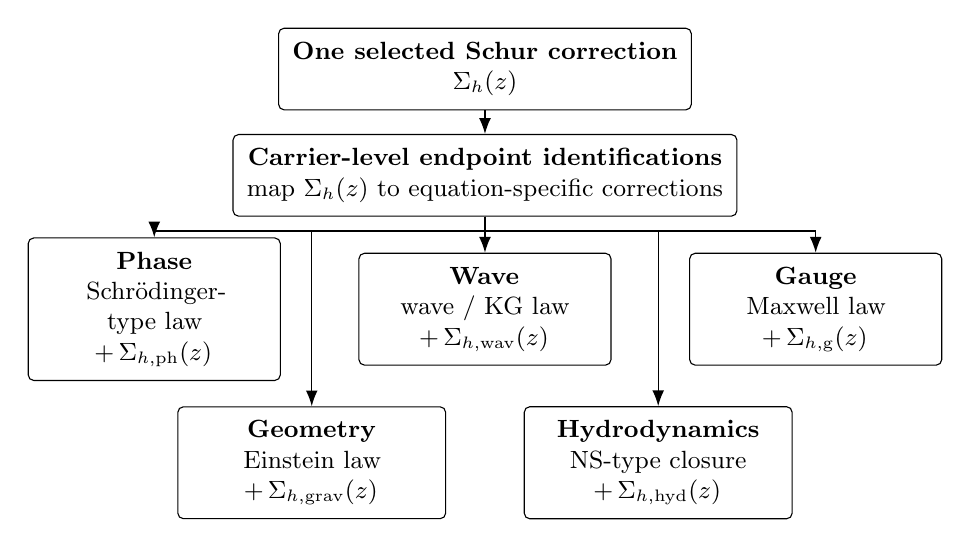
\begin{tikzpicture}[x=1cm,y=1cm]
  \node[ccbox, align=center, minimum width=5.2cm, minimum height=0.95cm] (schur) at (0,4.05)
    {\textbf{One selected Schur correction}\\\(\CCSigma{h}{z}\)};
  \node[ccbox, align=center, minimum width=5.8cm, minimum height=0.95cm] (id) at (0,2.7)
    {\textbf{Carrier-level endpoint identifications}\\map \(\CCSigma{h}{z}\) to equation-specific corrections};

  \draw[ccarrow, line width=0.5pt] (schur.south) -- (id.north);

  \node[ccbox, align=center, text width=2.85cm, minimum height=1.25cm] (ph) at (-4.2,1.0)
    {\textbf{Phase}\\Schr\"odinger-type law\\\(+\,\Sigma_{h,\mathrm{ph}}(z)\)};
  \node[ccbox, align=center, text width=2.85cm, minimum height=1.25cm] (wav) at (0,1.0)
    {\textbf{Wave}\\wave / KG law\\\(+\,\Sigma_{h,\mathrm{wav}}(z)\)};
  \node[ccbox, align=center, text width=2.85cm, minimum height=1.25cm] (gau) at (4.2,1.0)
    {\textbf{Gauge}\\Maxwell law\\\(+\,\Sigma_{h,\mathrm g}(z)\)};
  \node[ccbox, align=center, text width=3.05cm, minimum height=1.25cm] (geo) at (-2.2,-0.95)
    {\textbf{Geometry}\\Einstein law\\\(+\,\Sigma_{h,\mathrm{grav}}(z)\)};
  \node[ccbox, align=center, text width=3.05cm, minimum height=1.25cm] (hyd) at (2.2,-0.95)
    {\textbf{Hydrodynamics}\\NS-type closure\\\(+\,\Sigma_{h,\mathrm{hyd}}(z)\)};

  \draw[ccarrow, line width=0.5pt] (id.south) -- ++(0,-0.18) -| (ph.north);
  \draw[ccarrow, line width=0.5pt] (id.south) -- ++(0,-0.18) -- (wav.north);
  \draw[ccarrow, line width=0.5pt] (id.south) -- ++(0,-0.18) -| (gau.north);
  \draw[ccarrow, line width=0.5pt] (id.south) -- ++(0,-0.18) -| (geo.north);
  \draw[ccarrow, line width=0.5pt] (id.south) -- ++(0,-0.18) -| (hyd.north);
\end{tikzpicture}%
}
\caption{The common predictive structure of Part~II. One selected Schur
correction \(\CCSigma{h}{z}\) is carried through the endpoint identifications
to produce the equation-specific returned remainders. The recognizable textbook
laws are the lossless leading-order representatives obtained when those
corrections vanish.}
\label{fig:returned-remainder-surface}
\end{figure}

Four of those intrinsic equations already admit exact solved coherent models on
the present scope. For the wave equation,
Theorem~\ref{thm:hidden-channel-wave-remainder-and-branch-splitting} and its
corollaries compute the returned profile explicitly and identify exact branch
shifts, avoided crossing, and low-energy renormalization. For the phase equation,
Theorem~\ref{thm:hidden-channel-phase-remainder-and-spectral-splitting} and
Corollaries~\ref{cor:exact-off-resonant-phase-line-shifts},
\ref{cor:exact-avoided-crossing-coupled-phase-branches}, and
\ref{cor:low-energy-renormalized-phase-offset-and-transport-coefficient}
likewise compute the coherent returned phase profile on a two-channel model
and show exact spectral line shifts, branch repulsion, and low-energy
renormalization of the visible phase offset and transport coefficient. For the
gauge equation, Theorem~\ref{thm:hidden-channel-gauge-current-and-branch-splitting}
and Corollaries~\ref{cor:exact-off-resonant-gauge-pole-shifts},
\ref{cor:exact-avoided-crossing-coupled-gauge-branches}, and
\ref{cor:low-frequency-induced-exchange-susceptibility} compute the returned
gauge current on a two-channel model and show exact gauge-pole shifts, branch
repulsion, and low-frequency induced exchange susceptibility on the visible
gauge sector. For the geometric equation,
Theorem~\ref{thm:hidden-channel-geometric-remainder-and-branch-splitting} and
Corollaries~\ref{cor:exact-off-resonant-geometric-pole-shifts},
\ref{cor:exact-avoided-crossing-coupled-geometric-branches}, and
\ref{cor:low-frequency-induced-geometric-susceptibility} compute the returned
linearized geometric profile on a two-channel model and show exact
geometric-pole shifts, branch repulsion, and low-frequency induced
symmetric-response susceptibility on the visible geometric sector.

The theory does not identify a nonzero remainder with any named phenomenon in
advance. It does not, by itself, say
that a given correction is ``dark matter,'' ``quantum gravity,''
``decoherence,'' or ``turbulence.'' Those are concrete realization problems.
What the theory does say is sharper: on the present scope, any such
departure must enter through exact returned remainders or induced coefficient
scales on the same selected realization, not through ad hoc primitive source
terms foreign to the bundle. The explicit wave-speed correction and hard cutoff
above are the first concrete example of that predictive structure rather than the
last.

\subsection{Candidate Phenomenology of Returned Remainders}

The theorems above do not identify any nonzero returned remainder with a named
physical anomaly. They do provide a disciplined
phenomenology map: if a concrete realized family yields a nonzero equation-specific
correction \(\Sigma_{h,\bullet}(z)\), then the resulting observable departure
from the corresponding leading textbook law should fall into a restricted class
of signatures. Table~\ref{tab:returned-remainder-phenomenology} records that
map at the present level of rigor. It is intended as a hypothesis table for
future calculation and comparison, not as a proved identification theorem.

\begin{table}[ht]
\centering
\scriptsize
\setlength{\tabcolsep}{3pt}
\begin{tabular}{@{}P{1.6cm}P{2.7cm}P{4.7cm}P{4.5cm}@{}}
\toprule
Equation family & Correction & Observable signature & Comparison language \\
\midrule
Phase
& \(\Sigma_{h,\mathrm{ph}}(z)\)
& phase drift, line shifts, loss of clean interference, or effective
  environment-coupled evolution on the visible cut
& open-system correction, decoherence-type term, level-shift / self-energy
  correction \\

Wave
& \(\Sigma_{h,\mathrm{wav}}(z)\)
& nontrivial dispersion, nonlocal propagation, high-frequency slowdown, or
  cutoff behavior beyond the clean wave/Klein--Gordon form
& dispersive-medium correction, lattice/discrete propagation correction,
  effective wave self-energy; the nearest-neighbor specialization already gives
  a concrete subluminal high-energy correction and hard cutoff \\

Gauge
& \(\Sigma_{h,\mathrm g}(z)\)
& effective mismatch between visible current and clean Maxwell response,
  polarization-like medium effects, or unresolved exchange-current correction
& exchange-current correction, polarization / medium response,\newline
  vacuum-polarization-type effective term \\

Geometry
& \(\Sigma_{h,\mathrm{grav}}(z)\)
& additional effective stress-response on top of clean Einstein behavior,
  backreaction-like deviation, or visible source mismatch not captured by the
  leading geometric carrier
& effective stress-tensor correction, geometric backreaction,\newline
  dark-sector phenomenology at the level of the visible response law \\

Hydro\-dynamics
& \(\Sigma_{h,\mathrm{hyd}}(z)\)
& stress not captured by Newtonian viscosity, including memory, nonlocality,
  anisotropic closure, turbulent transfer, rarefied-gas correction, or
  non-Newtonian response
& Reynolds stress, LES subgrid stress,\newline Burnett / kinetic-memory
  correction,\newline non-Newtonian constitutive correction \\
\bottomrule
\end{tabular}
\caption{Hypothesis map for the returned-remainder structure. Each row is
conditional: if the corresponding selected Schur correction is nonzero on a
concrete realized family, the observable departure from the leading textbook
law should appear in the indicated signature class.}
\label{tab:returned-remainder-phenomenology}
\end{table}

The table is intentionally one level weaker than the proved intrinsic theorems.
It does not assert that any existing anomaly is already explained. It records
the restricted comparison classes suggested by the theory: compute the relevant
\(\Sigma_{h,\bullet}(z)\) on a concrete selected realization, then compare that
computed correction with the phenomenology in the corresponding row.

\subsection{Extensions}

\begin{enumerate}[leftmargin=1.2em, itemsep=0.3em]
\item \textbf{Further carrier classes and broader thermodynamic extension.} Additional
      mixed and many-body carriers belong naturally in the same
      physical-law-selection format. The present thermodynamic extension is now
      stronger than a first bookkeeping layer: returned flux, unrecovered
      stock, monotone irreversibility, selected-history entropy production, the
      selected-tower thermodynamic state space, its canonical entropy
      functional, and its exact equilibrium class are all mechanically forced
      on the selected cut. The broader thermodynamic program beyond that
      selected tower concerns extension to coarse-state spaces not
      canonically induced by the realized tower, local equilibrium and
      equilibrium manifolds there, and broader
      thermodynamic/macroscopic closure principles under explicit
      coarse-graining hypotheses.
      On the spectral side, the unit-balanced \(D=2\) seed defines a
      one-fiber reversible law with a single-channel monodromy/recursion
      stage, a primitive-support tower with prime-index maximal cyclic
      refinement, and a forced continuum spectral defect form
      \(\mathcal E_{\infty}^{\mathrm{prim}}\). Arithmetic realization would
      enter through the external identification theorem
      \(\mathcal E_{\infty}^{\mathrm{prim}} = W_{\xi}\).
\end{enumerate}

On the present scope, the remaining manuscript work is now largely
downstream rather than conceptual: extend the current carrier family, develop
broader effective closures, and compute quantitative remainder laws for the
intrinsic carriers within the same residual-return formalism.


% ============================================================
% APPENDICES
% ============================================================
\appendix
\makeatletter
\def\toclevel@subsection{2}
\def\toclevel@subsubsection{3}
\makeatother
\manuscriptpart{Appendices}{part.appendices}

The first group of appendices (A--G) collects proofs that have been moved from
the main text to keep the derivation chain readable. Each proof is labeled and
cross-referenced from the theorem statement it supports. The second group
collects supplementary operator-theoretic extensions and the formal
certification boundary.

\manuscriptappendix{Foundations Proofs (Chapters 1--2)}
% Appendix A: Foundations Proofs (Chapters 1--2)
\label{sec:appendix-foundations}

\begin{proof}[Proof of Theorem~\ref{thm:choice}]
\label{proof:thm:choice}
The Axiom of Choice (AC) asserts: for any collection of non-empty sets, there exists a function selecting one element from each. For \emph{infinite} collections, this requires a non-constructive principle.

In the finite setting of this paper:
\begin{enumerate}[label=(\roman*), itemsep=0.2em]
\item Every configuration is finite, already on the incidence-count surface.
\item Each finite family is represented together with an explicit enumeration of each fiber.
\item Given such an explicitly enumerated family, we construct a choice function by taking the first listed element at each index.
\end{enumerate}
The construction is explicit and constructive: once each finite fiber is enumerated, one simply selects the first listed element at each index. No global choice principle is used.
\end{proof}


\manuscriptappendix{Topology and Dimension Proofs (Chapters 3--4)}
% Appendix B: Topology and Dimension Proofs (Chapters 3--4)
\label{sec:appendix-topology}

\begin{proof}[Proof of Theorem~\ref{thm:closure-balance-realizes-interface}]
\label{proof:thm:closure-balance-realizes-interface}
Theorem~\ref{thm:forced-stable-dimension} identifies $D=4$ as the unique
nontrivial balanced dimension. Definition~\ref{def:closure-realized-state}
therefore gives the canonical nontrivial finite state space selected by the
counting bedrock, and Definition~\ref{def:closure-realized-pairing} equips it
with its canonical energy pairing. Theorem~\ref{thm:state-transport} shows that
the active state layer carries no additional data beyond that realized state.
Theorem~\ref{thm:true-boundary-realized} and
Theorem~\ref{thm:full-boundary-closes} provide the full nilpotent boundary.
Definition~\ref{def:coherence-tower}, Theorem~\ref{thm:realized-uniqueness},
and Lemma~\ref{lem:coherence-tower-faithful} provide the canonical tower and
its faithfulness. These are exactly the ingredients required by the structural
interface of Part~I.
\end{proof}

\begin{proof}[Proof of Theorem~\ref{thm:canonical-tail-laws}]
\label{proof:thm:canonical-tail-laws}
The explicit projection law gives
\[
\CCPi{0}x=0,\qquad
\CCPi{1}x=(x_0,0,0,0),\qquad
\CCPi{2}x=(x_0,x_1,0,0),
\]
\[
\CCPi{3}x=(x_0,x_1,x_2,0),\qquad
\CCPi{h}x=x \quad (h\ge 4).
\]
Hence the corresponding shadows are
\[
x-\CCPi{0}x=(x_0,x_1,x_2,x_3),\qquad
x-\CCPi{1}x=(0,x_1,x_2,x_3),
\]
\[
x-\CCPi{2}x=(0,0,x_2,x_3),\qquad
x-\CCPi{3}x=(0,0,0,x_3),\qquad
x-\CCPi{h}x=0 \quad (h\ge 4).
\]
Since the canonical energy is the coordinate sum of the signed-count energies,
the stated formulas for $E_h(x)$ follow immediately.

Likewise,
\[
(\CCPi{1}-\CCPi{0})x=(x_0,0,0,0),\quad
(\CCPi{2}-\CCPi{1})x=(0,x_1,0,0),
\]
\[
(\CCPi{3}-\CCPi{2})x=(0,0,x_2,0),\quad
(\CCPi{4}-\CCPi{3})x=(0,0,0,x_3),
\]
and $(\CCPi{h+1}-\CCPi{h})x=0$ for $h\ge 4$. Taking energies again gives the
formulas for $\mu_h(x)$.
\end{proof}

\begin{proof}[Proof of Theorem~\ref{thm:barrier-uniqueness}]
\label{proof:thm:barrier-uniqueness}
Direct computation gives
\[
\cH(2)=0,\qquad \cH(3)=1,\qquad \cH(4)=0.
\]
For $D=1$, one has $\cH(1)= -1$. It therefore remains to treat $D\ge 5$.
At $D=5$,
\[
\binom{5}{2}=10<24=4!.
\]
Assume now that $(D-1)!>\binom{D}{2}$ for some $D\ge 5$. Then
\[
D! = D(D-1)! > D\binom{D}{2} = \frac{D^2(D-1)}{2}.
\]
Since $D(D-1)>D+1$ for every $D\ge 3$, it follows that
\[
\frac{D^2(D-1)}{2} > \frac{D(D+1)}{2} = \binom{D+1}{2}.
\]
Hence $D!>\binom{D+1}{2}$, so by induction
\[
(D-1)!>\binom{D}{2}
\qquad\text{for all }D\ge 5.
\]
Therefore $\cH(D)<0$ for every $D\ge 5$, and the only positive value occurs at
$D=3$.
\end{proof}

\begin{proof}[Proof of Theorem~\ref{thm:unit-seed-and-six-slot-carrier}]
\label{proof:thm:unit-seed-and-six-slot-carrier}
Theorem~\ref{thm:forced-stable-dimension} shows that the only balanced
dimensions are $D=2$ and $D=4$. Direct computation gives
\[
N_{\mathrm{cl}}(2)=\binom{2}{2}=1!=1,
\qquad
N_{\mathrm{cl}}(4)=\binom{4}{2}=3!=6.
\]
The two conclusions are exactly these two values read as local balanced slot
counts.
\end{proof}

\begin{proof}[Proof of Corollary~\ref{cor:d2-primitive-support-profile}]
\label{proof:cor:d2-primitive-support-profile}
Fix \(C\in\mathcal C\). If \(C\) is primitive, take \(P=C\) and \(m=1\). If
\(C\) is a repeat, then by Definition~\ref{def:primitive-transport-cycle} it
has the form \(C=W^{\times m_1}\) for some shorter cycle \(W\) and some
\(m_1>1\). If \(W\) is primitive, set \(P=W\). Otherwise repeat the same
reduction on \(W\). Because cycle length strictly decreases at each nontrivial
repeat reduction, this process terminates at a primitive core \(P\). Repeated
application of Proposition~\ref{prop:repeat-cycle-monodromy-factorization}
then gives
\[
\mathcal M(C)=\mathcal M(P)^m
\]
for some \(m\ge 1\). Doing this for each \(C\in\mathcal C\) produces the
finite family \(\mathcal P\). Since
Corollary~\ref{cor:single-channel-unit-seed} shows that the seed admits only
one irreducible local channel, these repeat powers introduce no new seed
carrier type.
\end{proof}

\begin{proof}[Proof of Theorem~\ref{thm:finite-local-type-profiles}]
\label{proof:thm:finite-local-type-profiles}
Theorem~\ref{thm:barrier-uniqueness} identifies $D=3$ as the unique residual
dimension, and Theorem~\ref{thm:unit-seed-and-six-slot-carrier} identifies
$D=2$ and $D=4$ as the only balanced dimensions. Hence any passage from the
unit-balanced seed to the nontrivial balanced carrier crosses the unique
residual interface at $D=3$.

For $D=4$, Theorem~\ref{thm:unit-seed-and-six-slot-carrier} gives
$N_{\mathrm{cl}}(4)=6$. By Definition~\ref{def:local-type-profile}, every
local type profile on the balanced carrier is therefore a partition of $6$.
The displayed list is the complete constructive enumeration of those
partitions.
\end{proof}

\begin{proof}[Proof of Proposition~\ref{prop:symmetry-refined-logical-type}]
\label{proof:prop:symmetry-refined-logical-type}
Because the nonzero isotypic components form a direct-sum decomposition of the
six-dimensional carrier,
\[
6=\dim V=\sum_{\rho}\dim V_\rho,
\]
where every summand is a positive integer. This is exactly a partition of $6$,
proving (i). Since each nonzero isotypic component has dimension at least $1$,
there can be at most six such components, proving (ii). Statement (iii)
follows because Theorem~\ref{thm:finite-local-type-profiles} is precisely the
constructive enumeration of the partitions of $6$.
\end{proof}

\begin{proof}[Proof of Theorem~\ref{thm:intrinsic-six-slot-decomposition}]
\label{proof:thm:intrinsic-six-slot-decomposition}
Define the uniform vector
\[
u_0:=\sum_{1\le i<j\le 4} e_{ij},
\]
and set $U_1:=\bbR u_0$. This space is $S_4$-invariant because relabeling
permutes the six basis vectors.

Next define the three perfect-matching sums
\[
m_1:=e_{12}+e_{34},\qquad
m_2:=e_{13}+e_{24},\qquad
m_3:=e_{14}+e_{23}.
\]
Set
\[
U_2:=\Span\{m_1-m_2,\; m_1-m_3\}.
\]
Relabeling permutes the three perfect matchings, so $U_2$ is $S_4$-invariant.
Since $m_1-m_2$ and $m_1-m_3$ are linearly independent, $\dim U_2=2$.

Now define the four vertex-star vectors
\[
s_1:=e_{12}+e_{13}+e_{14},\qquad
s_2:=e_{12}+e_{23}+e_{24},
\]
\[
s_3:=e_{13}+e_{23}+e_{34},\qquad
s_4:=e_{14}+e_{24}+e_{34}.
\]
For $x=(x_1,x_2,x_3,x_4)\in\bbR^4$ with $x_1+x_2+x_3+x_4=0$, define
\[
\Phi(x):=\sum_{i=1}^4 x_i s_i.
\]
Set
\[
U_3:=\Phi\bigl(\{x\in\bbR^4:\ x_1+x_2+x_3+x_4=0\}\bigr).
\]
Because relabeling permutes the four stars, $U_3$ is $S_4$-invariant.
Moreover $\Phi(x)$ has edge coefficients $x_i+x_j$. If $\Phi(x)=0$, then
\[
x_1+x_2=x_1+x_3=x_2+x_3=0.
\]
Subtracting the first two equations gives $x_2=x_3$, and then
$x_2+x_3=0$ implies $x_2=x_3=0$. Hence $x_1=0$ from $x_1+x_2=0$, and finally
$x_4=0$ from $x_1+x_2+x_3+x_4=0$. Thus $\Phi$ is injective on the
three-dimensional hyperplane $\sum x_i=0$, so $\dim U_3=3$.

It remains to prove the sum is direct. Define the star-sum functional at
vertex $i$ by summing the coefficients on the three edges incident to $i$.
For every vector in $U_2$, each star sum is $0$, because the coefficients in
$m_1-m_2$ and $m_1-m_3$ cancel at every vertex. For $\Phi(x)\in U_3$, the star
sum at vertex $i$ equals
\[
2x_i+\sum_{j\ne i}x_j=x_i
\]
since $\sum_k x_k=0$. Therefore $U_2\cap U_3=\{0\}$.

Also $u_0\notin U_2$ because $u_0$ has nonzero star sums, while every vector of
$U_2$ has zero star sums. And $u_0\notin U_3$ because every vector of $U_3$
has star sums summing to $0$, whereas $u_0$ has star sum $3$ at each vertex.
Hence
\[
U_1\cap U_2=U_1\cap U_3=\{0\}.
\]
Since
\[
\dim U_1+\dim U_2+\dim U_3=1+2+3=6=\dim V_{\mathrm{slot}},
\]
the sum is direct and exhausts $V_{\mathrm{slot}}$.
\end{proof}

\begin{proof}[Proof of Theorem~\ref{thm:six-slot-carrier-is-symmetric-square-of-u3}]
\label{proof:thm:six-slot-carrier-is-symmetric-square-of-u3}
In the proof of Theorem~\ref{thm:intrinsic-six-slot-decomposition}, the channel
\(U_3\) is constructed as the image of the zero-sum hyperplane
\[
H:=\{x\in\bbR^4:\ x_1+x_2+x_3+x_4=0\}
\]
under the injective map
\[
\Phi(x)=\sum_{i=1}^4 x_i s_i.
\]
Thus \(\Phi\) identifies \(H\) canonically with \(U_3\).

Define a symmetric bilinear map on \(H\) by
\[
B(x,y):=\sum_{1\le i<j\le 4}(x_i y_j+x_j y_i)e_{ij}.
\]
Because the coefficient of \(e_{ij}\) is symmetric bilinear in \((x,y)\), the
map \(B\) is symmetric bilinear. Transport it to \(U_3\) through \(\Phi\): for
\(u=\Phi(x)\) and \(v=\Phi(y)\), set
\[
\beta_{\mathrm{slot}}(u,v):=B(x,y).
\]
Since \(\Phi\) is injective on \(H\), this is well-defined and symmetric
bilinear on \(U_3\times U_3\).

To prove that the image generates \(V_{\mathrm{slot}}\), fix any slot
\(\{i,j\}\in\mathcal S_4\) and let \(u_{ij}\in H\) be the vector with \(+1\) in
slot \(i\), \(-1\) in slot \(j\), and \(0\) elsewhere. Then
\[
B(u_{ij},u_{ij})=-2\,e_{ij}.
\]
Hence every basis vector \(e_{ij}\) lies in the image of \(B\), so the image of
\(\beta_{\mathrm{slot}}\) generates all of \(V_{\mathrm{slot}}\).

Because \(\beta_{\mathrm{slot}}\) is symmetric bilinear, the universal property
of the symmetric square yields a unique linear map
\[
\overline\beta_{\mathrm{slot}}:\mathrm{Sym}^2(U_3)\to V_{\mathrm{slot}}
\]
whose value on the class of \(u\otimes v\) is \(\beta_{\mathrm{slot}}(u,v)\).
The preceding paragraph shows that \(\overline\beta_{\mathrm{slot}}\) is
surjective. Since \(\dim U_3=3\),
\[
\dim \mathrm{Sym}^2(U_3)=\frac{3(3+1)}2=6,
\]
and Definition~\ref{def:local-slot-carrier} gives \(\dim V_{\mathrm{slot}}=6\).
Therefore a surjective linear map between these two six-dimensional spaces is
an isomorphism.

Finally, every ingredient in the construction is intrinsic: the hyperplane
\(H\), the map \(\Phi\), and the slot basis are all defined from the canonical
balanced four-incidence and its relabeling action. Hence the resulting
identification \(V_{\mathrm{slot}}\cong \mathrm{Sym}^2(U_3)\) is canonical and
compatible with intrinsic relabeling.
\end{proof}

\begin{proof}[Proof of Theorem~\ref{thm:intrinsic-slot-normal-form}]
\label{proof:thm:intrinsic-slot-normal-form}
Because $S_4$ acts transitively on the six slots, the diagonal coefficients
$A_{\alpha\alpha}$ are all equal; call the common value $a$.

Next consider off-diagonal ordered pairs $(\alpha,\beta)$ with
$\alpha\neq\beta$. Under the relabeling action of $S_4$, such pairs fall into
exactly two orbit types: adjacent and disjoint. Indeed, if two ordered pairs
share one primitive, a relabeling sends one to the other; if they are disjoint,
a relabeling again sends one to the other; and adjacency cannot be relabeled to
disjointness because the intersection size is preserved. Since $A$ commutes
with the action, its matrix coefficients are constant on each orbit type. Call
those constants $b$ on adjacent pairs and $c$ on disjoint pairs. This gives the
displayed formula.

Uniqueness of $a,b,c$ is immediate because the three slot-pair classes are
nonempty and disjoint.
\end{proof}

\begin{proof}[Proof of Corollary~\ref{cor:intrinsic-channel-eigenvalues}]
\label{proof:cor:intrinsic-channel-eigenvalues}
For the uniform vector
\[
u_0=\sum_{1\le i<j\le 4} e_{ij},
\]
each basis slot sees one diagonal contribution, four adjacent contributions,
and one disjoint contribution. Hence
\[
Au_0=(a+4b+c)u_0.
\]
So the one-dimensional channel is $A$-invariant with eigenvalue $\lambda_1$.

Now use the perfect-matching basis of Theorem~\ref{thm:intrinsic-six-slot-decomposition}:
\[
m_1=e_{12}+e_{34},\qquad
m_2=e_{13}+e_{24},\qquad
m_3=e_{14}+e_{23}.
\]
A direct substitution into the normal form gives
\[
A(m_1-m_2)=(a-2b+c)(m_1-m_2),
\]
\[
A(m_1-m_3)=(a-2b+c)(m_1-m_3).
\]
Therefore $A$ acts on the two-dimensional channel by the scalar
$\lambda_2=a-2b+c$.

Finally use the vertex-star differences
\[
s_1-s_2,\qquad s_1-s_3,\qquad s_1-s_4
\]
from the proof of Theorem~\ref{thm:intrinsic-six-slot-decomposition}. A direct
substitution again yields
\[
A(s_1-s_2)=(a-c)(s_1-s_2),\qquad
A(s_1-s_3)=(a-c)(s_1-s_3),\qquad
A(s_1-s_4)=(a-c)(s_1-s_4).
\]
Hence $A$ acts on the three-dimensional channel by the scalar
$\lambda_3=a-c$.
\end{proof}


\manuscriptappendix{Tower Calculus Proofs (Chapter 5)}
% Appendix C: Tower Calculus Proofs (Chapter 5)
\label{sec:appendix-tower}

% ============================================================
% Proofs from foundational_lemmas.tex
% ============================================================

\begin{proof}[Proof of Lemma~\ref{lem:block-splitting}]
\label{proof:lem:block-splitting}
Apply Lemma~\ref{lem:resolution-identity} to $B\CCPi{h}x$:
\[
\CCPi{h}AB\CCPi{h}
=
\CCPi{h}A(\CCPi{h} + \CCPibar{h})B\CCPi{h}
=
\CCPi{h}A\CCPi{h}B\CCPi{h} + \CCPi{h}A\CCPibar{h}B\CCPi{h}.
\]
The first term is the observed composition and the second is the cross-shadow correction.
\end{proof}

% ============================================================
% Proofs from hft.tex
% ============================================================

\begin{proof}[Proof of Lemma~\ref{lem:silent-leak}]
\label{proof:lem:silent-leak}
Take the rebuilt finite state space and let $\Pi$ project onto the first coordinate:
\[
\Pi(x_0,x_1,x_2,x_3) = (x_0,0,0,0).
\]
Let $d$ send the first coordinate into the second and annihilate the others:
\[
d(x_0,x_1,x_2,x_3) = (0,x_0,0,0).
\]
Then $d^2 = 0$. The observed operator $d_\Pi = \Pi d \Pi$ vanishes, so $d_\Pi^2 = 0$.
But $L(1,0,0,0) = (0,1,0,0) \neq 0$, while the return map vanishes on that shadow image, so $\delta = RL = 0$.
\end{proof}

% ============================================================
% Proofs from tower_calculus.tex
% ============================================================

\begin{proof}[Proof of Lemma~\ref{lem:tower-derivative-block}]
\label{proof:lem:tower-derivative-block}
On the $(h,k)$ block,
\[
\Delta_h \CCIndexOp A \Delta_k = h\, \CCBlock{A}{h}{k},
\qquad
\Delta_h A \CCIndexOp \Delta_k = k\, \CCBlock{A}{h}{k},
\]
so the commutator contributes the factor $(h-k)$. The Leibniz rule is the
usual commutator identity
\[
[\CCIndexOp, AB] = [\CCIndexOp, A]B + A[\CCIndexOp, B].
\]
\end{proof}

\begin{proof}[Proof of Proposition~\ref{prop:tower-order-arithmetic}]
\label{proof:prop:tower-order-arithmetic}
Statement (i) is immediate from the definition of block support.

For (ii), if $|j-k|>m+n$, then for every intermediate band index $\ell$ one has
either $|j-\ell|>m$ or $|\ell-k|>n$. Hence every term in the block expansion
\[
\CCDelta{j}AB\CCDelta{k}
=
\sum_{\ell}\CCDelta{j}A\CCDelta{\ell}B\CCDelta{k}
\]
vanishes, so $\CCDelta{j}AB\CCDelta{k}=0$.

For (iii), Lemma~\ref{lem:tower-derivative-block} gives
\[
\CCBlock{\CCDer{A}}{j}{k}=(j-k)\,\CCBlock{A}{j}{k}.
\]
Thus the block support of $\CCDer{A}$ is exactly the block support of $A$.
\end{proof}

\begin{proof}[Proof of Proposition~\ref{prop:transport-recursion-compatibility}]
\label{proof:prop:transport-recursion-compatibility}
For $g\in G$ and $x\in F^{\bbZ}$,
\[
(\mathcal R_B\mathcal U(g)x)_n
=
U(g)x_{n+1}-BU(g)x_n+U(g)x_{n-1}
=
U(g)(x_{n+1}-Bx_n+x_{n-1})
=
(\mathcal U(g)\mathcal R_Bx)_n,
\]
which proves (a). The same calculation with $J_F$ in place of $U(g)$ gives
\[
(\mathcal R_B\mathcal Jx)_n
=
J_Fx_{n+1}-BJ_Fx_n+J_Fx_{n-1}
=
J_F(x_{n+1}-Bx_n+x_{n-1})
=
(\mathcal J\mathcal R_Bx)_n,
\]
proving (b).

For (c), let $x,y$ be finitely supported sequences. Using the sum inner
product and shifting indices in the finite sums,
\begin{align*}
\langle \mathcal R_Bx,y\rangle
&=
\sum_n \langle x_{n+1},y_n\rangle
-\sum_n \langle Bx_n,y_n\rangle
+\sum_n \langle x_{n-1},y_n\rangle \\
&=
\sum_n \langle x_n,y_{n-1}\rangle
-\sum_n \langle x_n,B^*y_n\rangle
+\sum_n \langle x_n,y_{n+1}\rangle \\
&=
\sum_n \langle x_n,y_{n-1}-By_n+y_{n+1}\rangle \\
&=
\langle x,\mathcal R_By\rangle,
\end{align*}
because $B=B^*$.
\end{proof}

\begin{proof}[Proof of Proposition~\ref{prop:repeat-cycle-monodromy-factorization}]
\label{proof:prop:repeat-cycle-monodromy-factorization}
By definition, the monodromy of \(W^{\times m}\) is the product of the same
block \(T_r\cdots T_1\) repeated \(m\) times. Associativity of composition gives
\[
\mathcal M(W^{\times m})
=
(T_r\cdots T_1)\cdots(T_r\cdots T_1)
=
\mathcal M(W)^m.
\]
The final statement is exactly this factorization.
\end{proof}

\begin{proof}[Proof of Proposition~\ref{prop:cyclic-refinement-prime-step}]
\label{proof:prop:cyclic-refinement-prime-step}
Since \(H\) is a subgroup of a cyclic group, it is itself cyclic. Write
\[
H\cong C_m
\]
for some \(m\). Subgroups of a cyclic group correspond to divisors of its
order. If \(H'\subsetneq H\) is maximal, then there is no intermediate
subgroup, equivalently no divisor strictly between \(|H'|\) and \(|H|\).
Therefore the quotient \(|H|/|H'|\) has no nontrivial factor and must be
prime. Since \([H:H']=|H|/|H'|\), the index is prime.
\end{proof}

\begin{proof}[Proof of Theorem~\ref{thm:cyclic-refinement-prime-invariant}]
\label{proof:thm:cyclic-refinement-prime-invariant}
Let
\[
C_k=H_0\supset H_1\supset\cdots\supset H_r=\{0\}
\]
be a maximal refinement chain. Taking orders gives
\[
k=|C_k|=\prod_{i=0}^{r-1}\frac{|H_i|}{|H_{i+1}|}
=
\prod_{i=0}^{r-1}[H_i:H_{i+1}].
\]
By Proposition~\ref{prop:cyclic-refinement-prime-step}, each factor is prime.
Because \(C_k\) is cyclic, for every divisor \(d\mid k\) there is a unique
subgroup of order \(d\). Hence a maximal refinement chain is exactly a strict
descending divisor chain with no intermediate divisor steps, so its step
indices are prime and their product is \(k\). The uniqueness of the multiset of
prime factors of \(k\) therefore implies that every maximal cyclic refinement
chain has the same multiset of prime indices, up to permutation.
\end{proof}

\begin{proof}[Proof of Theorem~\ref{thm:isotropic-quadratic-transport}]
\label{proof:thm:isotropic-quadratic-transport}
Because $B$ commutes with the orthogonal action $U(g)$, the operator $B^*B$
also commutes with every $U(g)$. It is self-adjoint by construction. Since the
representation of $K$ on $F$ is irreducible, Corollary~\ref{cor:self-adjoint-commutant-scalarization}
forces every self-adjoint operator commuting with the action to be a scalar
multiple of the identity. Thus
\[
B^*B=\kappa(B)\,I_F
\]
for a unique real scalar $\kappa(B)$. Positivity of $B^*B$ implies
$\kappa(B)\ge 0$. The energy formula is then immediate.
\end{proof}

\begin{proof}[Proof of Theorem~\ref{thm:sphere-transitive-implies-irreducible}]
\label{proof:thm:sphere-transitive-implies-irreducible}
Suppose $W\subseteq F$ is a nonzero proper $K$-invariant subspace. Choose a
unit vector $w\in W$. Since $W$ is proper, there exists a unit vector
$v\in W^{\perp}$. By sphere transitivity, there exists $g\in K$ such that
\[
U(g)w=v.
\]
But $W$ is $K$-invariant, so $U(g)w\in W$, hence $v\in W\cap W^{\perp}$, which
forces $v=0$. This contradicts the choice of $v$ as a unit vector. Therefore
no nonzero proper invariant subspace exists, and $F$ is irreducible.
\end{proof}

\begin{proof}[Proof of Theorem~\ref{thm:metric-isotropic-quadratic-scalar}]
\label{proof:thm:metric-isotropic-quadratic-scalar}
Choose an orthonormal basis $\{e_i\}_{i=1}^m$ of $F$. By metric isotropy,
\[
\langle Qe_i,e_i\rangle=\kappa(Q)
\qquad(i=1,\dots,m).
\]
Thus every diagonal coefficient of $Q$ in this basis equals $\kappa(Q)$.

For $i\neq j$, the unit vector
\[
u_{ij}^{+}:=\frac{e_i+e_j}{\sqrt2}
\]
satisfies
\[
\kappa(Q)=\langle Qu_{ij}^{+},u_{ij}^{+}\rangle
=
\frac12\langle Qe_i,e_i\rangle
\frac12\langle Qe_j,e_j\rangle
\langle Qe_i,e_j\rangle
=
\kappa(Q)+\langle Qe_i,e_j\rangle.
\]
Hence
\[
\langle Qe_i,e_j\rangle=0
\qquad(i\neq j).
\]
So the matrix of $Q$ in the orthonormal basis $\{e_i\}$ is diagonal with every
diagonal entry equal to $\kappa(Q)$, which means
\[
Q=\kappa(Q)\,I_F.
\]
\end{proof}

\begin{proof}[Proof of Theorem~\ref{thm:transitive-direction-isotropy}]
\label{proof:thm:transitive-direction-isotropy}
For $g\in K$,
\[
U(g)QU(g)^*
=
\sum_{\alpha\in\mathcal D} q_{\alpha}\,U(g)\Pi_{\alpha}U(g)^*
=
\sum_{\alpha\in\mathcal D} q_{\alpha}\,\Pi_{g\cdot\alpha}.
\]
Because $Q$ commutes with the action, this must equal
\[
Q=\sum_{\alpha\in\mathcal D} q_{\alpha}\Pi_{\alpha}.
\]
Since the group acts transitively on $\mathcal D$, the coefficients are
constant on the orbit and hence there exists a real number $q$ such that
\[
q_{\alpha}=q
\qquad(\alpha\in\mathcal D).
\]
Therefore
\[
Q=q\sum_{\alpha\in\mathcal D}\Pi_{\alpha}=qc\,I_F.
\]
Setting $\kappa(Q):=qc$ gives the claim, and uniqueness is immediate.
\end{proof}

\begin{proof}[Proof of Theorem~\ref{thm:quadratic-transport-rigidity}]
\label{proof:thm:quadratic-transport-rigidity}
If $B$ carries data of type (i), the conclusion is exactly
Theorem~\ref{thm:isotropic-quadratic-transport}. If it carries data of type
(ii), the conclusion is exactly
Corollary~\ref{cor:sphere-transitive-quadratic-transport}. If it carries data
of type (iii), the conclusion is exactly
Corollary~\ref{cor:full-orthogonal-quadratic-transport}. If it carries data of
type (iv), the conclusion is exactly
Corollary~\ref{cor:metric-isotropic-transport}. Finally, if it carries data of
type (v), the conclusion is exactly
Corollary~\ref{cor:direction-frame-quadratic-coefficient}. In every case
$B^*B$ is positive semidefinite, so the scalar $\kappa(B)$ is nonnegative, and
uniqueness is immediate.
\end{proof}

\begin{proof}[Proof of Theorem~\ref{thm:orbit-generated-direction-frame}]
\label{proof:thm:orbit-generated-direction-frame}
By construction, each $\Pi_{\alpha}$ is a rank-one orthogonal projection and
the group acts transitively on the orbit $\mathcal D$. Define
\[
S:=\sum_{\alpha\in\mathcal D}\Pi_{\alpha}.
\]
Since the family is a single orbit, $S$ commutes with the orthogonal action of
$K$. It is also self-adjoint. Because $(F,U)$ is an isotropic transport
channel, the representation of $K$ on $F$ is irreducible. Therefore
Corollary~\ref{cor:self-adjoint-commutant-scalarization} forces
\[
S=c\,I_F
\]
for some real scalar $c$. Taking traces gives
\[
|\mathcal D|
=
\sum_{\alpha\in\mathcal D}\operatorname{Tr}(\Pi_{\alpha})
=
\operatorname{Tr}(S)
=
c\,\dim F,
\]
because each rank-one projection has trace $1$. Hence
\[
c=\frac{|\mathcal D|}{\dim F}.
\]
This proves both statements.
\end{proof}

\begin{proof}[Proof of Theorem~\ref{thm:ftc-tower}]
\label{proof:thm:ftc-tower}
If $h=k$, the right-hand side has block $\CCBlock{A}{h}{h}$. If $h \neq k$,
Lemma~\ref{lem:tower-derivative-block} gives
\[
\CCBlock{(\CCInt{\CCDer{A}})}{h}{k}
=
\frac{1}{h-k}\, \CCBlock{\CCDer{A}}{h}{k}
=
\frac{1}{h-k}(h-k)\, \CCBlock{A}{h}{k}
=
\CCBlock{A}{h}{k}.
\]
So every block agrees.
\end{proof}

\begin{proof}[Proof of Proposition~\ref{prop:tower-ibp}]
\label{proof:prop:tower-ibp}
Using the block formula from Lemma~\ref{lem:tower-derivative-block},
\[
\Tr(\CCDer{A}\, B)
=
\sum_{h,k} (h-k)\, \Tr(\CCBlock{A}{h}{k}\CCBlock{B}{k}{h}),
\]
while
\[
\Tr(A\, \CCDer{B})
=
\sum_{h,k} (k-h)\, \Tr(\CCBlock{A}{h}{k}\CCBlock{B}{k}{h}).
\]
The two sums are negatives of each other.
\end{proof}

% ============================================================
% Proofs from defect_rules.tex
% ============================================================

\begin{proof}[Proof of Proposition~\ref{prop:product-rule}]
\label{proof:prop:product-rule}
Decompose $x = \CCPi{h} x + \CCPibar{h} x$ and $y = \CCPi{h} y + \CCPibar{h} y$.
By bilinearity,
\begin{align*}
B(x,y) &= B(\CCPi{h} x + \CCPibar{h} x,\, \CCPi{h} y + \CCPibar{h} y) \\
&= B(\CCPi{h} x, \CCPi{h} y) + B(\CCPi{h} x, \CCPibar{h} y) + B(\CCPibar{h} x, \CCPi{h} y) + B(\CCPibar{h} x, \CCPibar{h} y).
\end{align*}
Apply $\CCPi{h}$ and use the closure condition $\CCPi{h} B(\CCPi{h} x, \CCPi{h} y) = B(\CCPi{h} x, \CCPi{h} y)$:
\begin{align*}
\CCTauBi{h}{B}{x}{y} &= \CCPi{h} B(x,y) - B(\CCPi{h} x, \CCPi{h} y) \\
&= B(\CCPi{h} x, \CCPi{h} y) + \CCPi{h} B(\CCPi{h} x, \CCPibar{h} y) + \CCPi{h} B(\CCPibar{h} x, \CCPi{h} y) + \CCPi{h} B(\CCPibar{h} x, \CCPibar{h} y) - B(\CCPi{h} x, \CCPi{h} y)\\
&= \CCPi{h} B(\CCPi{h} x, \CCPibar{h} y) + \CCPi{h} B(\CCPibar{h} x, \CCPi{h} y) + \CCPi{h} B(\CCPibar{h} x, \CCPibar{h} y). \qedhere
\end{align*}
\end{proof}

% ============================================================
% Proofs from constraint_compiler.tex
% ============================================================

\begin{proof}[Proof of Theorem~\ref{thm:compiler-contract}]
\label{proof:thm:compiler-contract}
This is a schema theorem asserting that the calculus provides a compositional route to a well-posed completion constraint.
\begin{itemize}[itemsep=0.1em]
\item Defect propagation (Section~\ref{sec:defect-rules}) composes via chain/product rules, yielding a derived defect contribution.
\item Elimination (Section~\ref{sec:resolvent-defect}) produces residual terms (Schur corrections) on the observable space.
\item These contributions aggregate into a ``required lower bound'' $D$ for stability.
\item Admissibility (Definition~\ref{def:admissibility}) selects completions $Q$ satisfying $D + Q \succeq 0$ that are minimal in PSD order.
\item Minimality in a partial order either yields a unique minimum or a minimal face (non-uniqueness certificate).
\end{itemize}
The theorem does not claim uniqueness of $D$; it states that once a bound is fixed, the completion constraint and certificate mechanism are canonical.
\end{proof}

\begin{proof}[Proof of Proposition~\ref{prop:operator-norm-selector-exists}]
\label{proof:prop:operator-norm-selector-exists}
By Definition~\ref{def:minimal-scalar-repair}, the operator
\[
\nu(D)I_{\mathcal K}
\]
is admissible, so the admissible set
\[
\mathcal A
:=
\{Q\in\mathcal Q: D+Q\succeq 0\}
\]
is nonempty. It is closed because the positive semidefinite cone is closed and
$Q\mapsto D+Q$ is continuous. Since $\mathcal Q$ is finite-dimensional, any
norm-minimizing sequence in $\mathcal A$ is bounded and therefore has a
convergent subsequence whose limit still lies in $\mathcal A$. Continuity of
the operator norm gives a minimizer.
\end{proof}

\begin{proof}[Proof of Theorem~\ref{thm:minimal-selectors-vanish}]
\label{proof:thm:minimal-selectors-vanish}
By Definition~\ref{def:minimal-scalar-repair}, the scalar correction
\[
\nu(D_h)I_{\CCPi{h}\cH}
\]
is admissible. Since $C_h^\ast$ minimizes operator norm among admissible
corrections,
\[
\|C_h^\ast\|
\le
\|\nu(D_h)I_{\CCPi{h}\cH}\|
=
\nu(D_h),
\]
proving (i). For $x\in\cH$,
\[
\|C_h^\ast \CCPi{h}x\|
\le
\|C_h^\ast\|\,\|\CCPi{h}x\|
\le
\nu(D_h)\,\|\CCPi{h}x\|.
\]
Because $\CCPi{h}$ is an orthogonal projection, $\|\CCPi{h}x\|\le \|x\|$, and
since $\nu(D_h)\to 0$, statement (ii) follows. Statement (iii) is exactly
Theorem~\ref{thm:selected-schur-recovery-general}.
\end{proof}

\begin{proof}[Proof of Theorem~\ref{thm:normal-form}]
\label{proof:thm:normal-form}
Each isotypic projector $P_\rho$ is constructed from the group action via $P_\rho = \frac{d_\rho}{|G|} \sum_{g \in G} \overline{\chi_\rho(g)}\, U(g)$, so $P_\rho$ commutes with every $U(g)$.
Since $A$ commutes with every $U(g)$ by hypothesis, $A$ commutes with $P_\rho$.

For distinct irreps $\rho \ne \rho'$, orthogonality of characters gives $P_\rho P_{\rho'} = 0$.
Thus:
\[
P_\rho \, A \, P_{\rho'} = P_\rho \, P_{\rho'} \, A = 0 \cdot A = 0.
\]
Since $\sum_\rho P_\rho = I$ on $\cH_{\mathrm{obs}}$, we have $A = \sum_{\rho, \rho'} P_\rho A P_{\rho'} = \sum_\rho P_\rho A P_\rho$.
\end{proof}

\begin{proof}[Proof of Theorem~\ref{thm:equivariant-coupling-decomposition}]
\label{proof:thm:equivariant-coupling-decomposition}
Let $P_\rho^X$ and $P_\rho^Y$ be the isotypic projectors for $X$ and $Y$.
Because $T$ intertwines the $G$-actions, it commutes with the projector
construction on both sides:
\[
P_\rho^Y T = T P_\rho^X
\qquad\text{for every }\rho.
\]
If $\rho\neq \rho'$, then orthogonality of isotypic projectors gives
\[
P_\rho^Y T P_{\rho'}^X = P_\rho^Y P_{\rho'}^Y T = 0,
\]
so $T$ is block-diagonal across isotypic channels:
\[
T=\sum_\rho P_\rho^Y T P_\rho^X.
\]
On the $\rho$-channel, Schur's lemma gives the standard normal form
\[
P_\rho^Y T P_\rho^X \cong I_{V_\rho}\otimes T_\rho
\]
for a unique linear map $T_\rho:M_\rho^X\to M_\rho^Y$. This proves the stated
decomposition.

For the dimension formula, each block contributes
\[
\dim \mathrm{Hom}_G(V_\rho\otimes M_\rho^X,\;V_\rho\otimes M_\rho^Y)
=
(\dim M_\rho^X)(\dim M_\rho^Y)\,\dim \mathrm{End}_G(V_\rho),
\]
and the block decomposition is a direct sum across $\rho$. Summing over the
appearing channels gives the stated formula.
\end{proof}

\begin{proof}[Proof of Theorem~\ref{thm:multiplicity-free-closures-scalar}]
\label{proof:thm:multiplicity-free-closures-scalar}
By Corollary~\ref{cor:isotypic-block}, every $G$-equivariant operator on the
$\rho$-isotypic component has the form
\[
P_{\rho}AP_{\rho}\cong I_{V_{\rho}}\otimes B_{\rho}
\]
for some operator $B_{\rho}$ on the multiplicity space $M_{\rho}$. If the
representation is multiplicity-free, then $\dim M_{\rho}=1$ for every appearing
$\rho$. Hence each $B_{\rho}$ is multiplication by a real scalar
$\lambda_{\rho}$ because $A$ is self-adjoint. Therefore $A$ is scalar on every
channel, which is exactly Definition~\ref{def:symmetry-scalar-closure}.
\end{proof}

\begin{proof}[Proof of Theorem~\ref{thm:orthogonal-symmetric-tensor-scalarization}]
\label{proof:thm:orthogonal-symmetric-tensor-scalarization}
Because $QIQ^\top=I$ for every $Q\in O(d)$, the equivariance relation gives
\[
L(I)=Q\,L(I)\,Q^\top
\qquad\text{for every }Q\in O(d).
\]
Thus $L(I)$ is fixed by every orthogonal conjugation, so there is a unique
scalar $\beta$ with
\[
L(I)=\beta I.
\]

For $i<j$, let
\[
F_{ij}:=E_{ij}+E_{ji},
\qquad
D_{ij}:=E_{ii}-E_{jj},
\]
where $E_{ab}$ are the standard matrix units. First consider $F_{12}$. Let
$R_1=\operatorname{diag}(-1,1,\dots,1)$ and
$R_2=\operatorname{diag}(1,-1,1,\dots,1)$. Then
\[
R_1F_{12}R_1^\top=-F_{12},
\qquad
R_2F_{12}R_2^\top=-F_{12}.
\]
Equivariance therefore yields
\[
R_1L(F_{12})R_1^\top=-L(F_{12}),
\qquad
R_2L(F_{12})R_2^\top=-L(F_{12}).
\]
These sign conditions force $L(F_{12})$ to have support only in the
$(1,2)$ and $(2,1)$ entries, hence
\[
L(F_{12})=a_{12}F_{12}
\]
for some scalar $a_{12}$. By permutation equivariance, the same scalar occurs
for every $F_{ij}$, so there is $\alpha\in\bbR$ with
\[
L(F_{ij})=\alpha F_{ij}
\qquad\text{for all }i<j.
\]

Now consider $D_{12}$. Every diagonal sign flip fixes $D_{12}$, so $L(D_{12})$
is fixed by all diagonal sign conjugations. Therefore $L(D_{12})$ is diagonal.
Permutations of coordinates $3,\dots,d$ show that all diagonal entries outside
the first two are equal, so
\[
L(D_{12})=\operatorname{diag}(a,b,c,\dots,c).
\]
Let $P_{12}$ be the permutation matrix exchanging coordinates $1$ and $2$.
Because
\[
P_{12}D_{12}P_{12}^\top=-D_{12},
\]
equivariance gives
\[
P_{12}L(D_{12})P_{12}^\top=-L(D_{12}).
\]
Thus $b=-a$ and $c=0$, hence
\[
L(D_{12})=aD_{12}.
\]
Let $Q_{\pi/4}$ be the rotation by $\pi/4$ in the $(1,2)$-plane. A direct
calculation gives
\[
Q_{\pi/4}D_{12}Q_{\pi/4}^\top=F_{12}.
\]
Equivariance then yields
\[
L(F_{12})
=
L(Q_{\pi/4}D_{12}Q_{\pi/4}^\top)
=
Q_{\pi/4}L(D_{12})Q_{\pi/4}^\top
=
aF_{12}.
\]
Since already $L(F_{12})=\alpha F_{12}$, one has $a=\alpha$. By permutation
equivariance,
\[
L(D_{ij})=\alpha D_{ij}
\qquad\text{for all }i<j.
\]

The matrices $\{F_{ij}\}_{i<j}$ together with the differences
$\{D_{ij}\}_{i<j}$ span the traceless symmetric carrier
$\mathrm{Sym}^2_0(\bbR^d)$. Hence
\[
L(S_0)=\alpha S_0
\qquad\text{for every }S_0\in \mathrm{Sym}^2_0(\bbR^d).
\]
Every symmetric tensor decomposes uniquely as
\[
S=\Bigl(S-\frac{\operatorname{tr}(S)}{d}I\Bigr)
+\frac{\operatorname{tr}(S)}{d}I
\]
with traceless part and trace part. Using the formulas above gives
\[
L(S)
=
\alpha\Bigl(S-\frac{\operatorname{tr}(S)}{d}I\Bigr)
+
\beta\,\frac{\operatorname{tr}(S)}{d}I.
\]
Uniqueness of $\alpha$ and $\beta$ follows from the direct-sum decomposition
\[
\mathrm{Sym}^2(\bbR^d)=\mathrm{Sym}^2_0(\bbR^d)\oplus \bbR I.
\qedhere
\]
\end{proof}

\begin{proof}[Proof of Theorem~\ref{thm:symmetry-reduction-admissibility}]
\label{proof:thm:symmetry-reduction-admissibility}
(i) Equivariant operators preserve isotypic components: $P_\rho A P_{\rho'} = 0$ for $\rho \ne \rho'$ when $A \in \mathrm{End}_G(\cH_{\mathrm{obs}})$.

(ii) For $x = \sum_\rho x_\rho$ with $x_\rho \in \cH_\rho$,
\[
\langle x, (D + Q) x \rangle = \sum_\rho \langle x_\rho, (D_\rho + Q_\rho) x_\rho \rangle.
\]
This is nonnegative for all $x$ iff each block summand is nonnegative.

(iii) Suppose $Q' \in \mathrm{End}_G(\cH_{\mathrm{obs}})$ satisfies $Q' \preceq Q$ with $D + Q' \succeq 0$.
Then $Q'_\rho \preceq Q_\rho$ and $D_\rho + Q'_\rho \succeq 0$ for each $\rho$.
Minimality of $Q_\rho$ forces $Q'_\rho = Q_\rho$, hence $Q' = Q$.
The converse assembles blockwise minima into a global minimum.

(iv) If $\langle x_*, (D + Q) x_* \rangle = 0$ with $x_* = \sum_\rho x_{*,\rho}$, then each summand $\langle x_{*,\rho}, (D_\rho + Q_\rho) x_{*,\rho} \rangle = 0$ (nonnegative terms summing to zero).
Any nonzero $x_{*,\rho}$ is a tight mode.
Minimal faces factor because the PSD cone in $\mathrm{End}_G(\cH_{\mathrm{obs}})$ is the product of PSD cones in each $\mathrm{End}_G(\cH_\rho)$.
\end{proof}

\begin{proof}[Proof of Theorem~\ref{thm:minimal-admissible-transport-order}]
\label{proof:thm:minimal-admissible-transport-order}
Because every admissible candidate has finite transport order, the set
\[
\{\operatorname{ord}_{\mathcal T}(A):A\in\mathcal F_{\mathrm{adm}}\}
\subseteq \bbN
\]
is nonempty. Every nonempty subset of $\bbN$ has a least element, which is
exactly $m_\ast$, proving (i). Statement (ii) is then just the definition of
the minimal-order admissible subclass. Statement (iii) follows because once the
minimal admissible order class has only one equivalence class, no second
inequivalent admissible candidate of the same minimal order remains.
\end{proof}

\begin{proof}[Proof of Theorem~\ref{thm:transport-generation-forces-scalar-recursion}]
\label{proof:thm:transport-generation-forces-scalar-recursion}
By item (i) of
Definition~\ref{def:transport-generated-admissible-family},
Theorem~\ref{thm:order-one-forcing-criterion} gives
\[
m_\ast=1.
\]
By item (iii) of
Definition~\ref{def:transport-generated-admissible-family},
Corollary~\ref{cor:no-preferred-direction-quadratic-transport} gives a unique
scalar $\kappa(B)\ge 0$ such that
\[
B^*B=\kappa(B)\,I_F.
\]
Finally, Theorem~\ref{thm:reversible-transport-recursion} gives the recursion
identity
\[
\mathcal R_Bx=0
\qquad\Longleftrightarrow\qquad
x_{n+1}=Bx_n-x_{n-1}
\]
for every bi-infinite sequence propagated by $B$. This proves all three
statements.
\end{proof}

% ============================================================
% Proofs from admissibility.tex
% ============================================================

\begin{proof}[Proof of Theorem~\ref{thm:scalar-completion}]
\label{proof:thm:scalar-completion}
(i) The condition $D + \nu L \succeq 0$ means $\langle x, (D + \nu L) x \rangle \ge 0$ for all $x$.
For $x \in \Ker(L)$, this reduces to $\langle x, D x \rangle \ge 0$, which holds by kernel compatibility.
For $x \notin \Ker(L)$, we have $\langle x, L x \rangle > 0$, so
\[
\langle x, (D + \nu L) x \rangle \ge 0
\quad\Leftrightarrow\quad
\nu \ge \frac{-\langle x, D x \rangle}{\langle x, L x \rangle}.
\]
Taking the supremum over all such $x$ gives the threshold $\nu_*$.

(ii) Since $\nu \mapsto \nu L$ is monotone in PSD order, $\nu_*$ is the unique minimal $\nu$ satisfying (i).

(iii) The maximizer $x_*$ achieves equality in the Rayleigh quotient, so $\langle x_*, (D + \nu_* L) x_* \rangle = 0$.
\end{proof}


\manuscriptappendix{Elimination and Solver Proofs (Chapter 6)}
% Appendix D: Elimination and Solver Proofs (Chapter 6)
\label{sec:appendix-elimination}

%%% --- resolvent_defect.tex proofs ---

\begin{proof}[Proof of Theorem~\ref{thm:feshbach-schur}]
\label{proof:thm:feshbach-schur}
Write the block form of $(I - zA)$:
\[
I - zA = \begin{pmatrix} I - z \CCBlockPP{A} & -z \CCBlockPQ{A} \\ -z \CCBlockQP{A} & I - z \CCBlockQQ{A} \end{pmatrix}.
\]
The Schur complement formula for block matrix inversion gives:
\[
\bigl[(I - zA)^{-1}\bigr]_{PP}
= \bigl( (I - z \CCBlockPP{A}) - (-z \CCBlockPQ{A})(I - z \CCBlockQQ{A})^{-1}(-z \CCBlockQP{A}) \bigr)^{-1}.
\]
Simplifying:
\[
\bigl[(I - zA)^{-1}\bigr]_{PP}
= \bigl( I - z \CCBlockPP{A} - z^2 \CCBlockPQ{A}(I - z \CCBlockQQ{A})^{-1} \CCBlockQP{A} \bigr)^{-1}
= \bigl( I - z \CCAeff{A}{P}(z) \bigr)^{-1}.
\]
Since $P (I - zA)^{-1} P$ acts as $[(I-zA)^{-1}]_{PP}$ on $\cH_P$, the identity follows.
\end{proof}

\begin{proof}[Proof of Proposition~\ref{prop:return-residual-is-schur}]
\label{proof:prop:return-residual-is-schur}
By Definition~\ref{def:residual-return-field},
\[
\mathcal F^{\mathrm{return}}_{P,A,z}(u)
=
\CCTransIn{P}R_Q\CCTransOut{P}u.
\]
Substituting
\[
\CCTransIn{P}=\CCBlockPQ{A},
\qquad
\CCTransOut{P}=\CCBlockQP{A}
\]
from Definition~\ref{def:residual-signature} gives
\[
\mathcal F^{\mathrm{return}}_{P,A,z}(u)
=
\CCBlockPQ{A}(I-z\CCBlockQQ{A})^{-1}\CCBlockQP{A}u
=
\CCSigmaP{P}{z}u.
\]
\end{proof}

%%% --- observable_relative_closure.tex proofs ---

\begin{proof}[Proof of Proposition~\ref{prop:typed-bilinear-defect-decomposition}]
\label{proof:prop:typed-bilinear-defect-decomposition}
Because \(I=P_X+Q_X\) and \(I=P_Y+Q_Y\),
\begin{align*}
B(y,x)
&=
B(P_Yy+Q_Yy,\ P_Xx+Q_Xx) \\
&=
B(P_Yy,P_Xx)
+
B(P_Yy,Q_Xx)
+
B(Q_Yy,P_Xx)
+
B(Q_Yy,Q_Xx).
\end{align*}
Applying \(P_Z\) and using the visible-visible closure condition gives
\begin{align*}
P_ZB(y,x)
&=
B(P_Yy,P_Xx)
+
P_ZB(P_Yy,Q_Xx) \\
&\qquad
+
P_ZB(Q_Yy,P_Xx)
+
P_ZB(Q_Yy,Q_Xx).
\end{align*}
Subtracting \(B(P_Yy,P_Xx)\) from both sides is exactly the claimed identity.
\end{proof}

\begin{proof}[Proof of Theorem~\ref{thm:schur-transport-jet-order}]
\label{proof:thm:schur-transport-jet-order}
Because $\CCPi{h}$ and $\CCPibar{h}$ are diagonal in the tower bands, they have
tower transport order $0$. Statement (i) therefore follows from
Proposition~\ref{prop:tower-order-arithmetic}(ii): the product
$\CCPi{h}A\CCPi{h}$ has the same order bound as $A$.

For $n\ge1$, the coefficient $K_{h,n}(A)$ is a product of $n+1$ copies of $A$
and diagonal order-$0$ projectors:
\[
K_{h,n}(A)
=
\CCPi{h}A(\CCPibar{h}A\CCPibar{h})^{n-1}\CCPibar{h}A\CCPi{h}.
\]
Repeatedly applying Proposition~\ref{prop:tower-order-arithmetic}(ii) shows
that each multiplication by a copy of $A$ increases the order bound by at most
$r$, while multiplication by $\CCPi{h}$ or $\CCPibar{h}$ does not increase the
order at all. Hence $K_{h,n}(A)$ has order at most $(n+1)r$.

Statement (iii) is then exactly the expansion of
Definition~\ref{def:schur-transport-jet} together with the coefficient bounds
just proved.
\end{proof}

\begin{proof}[Proof of Theorem~\ref{thm:observable-schur-jet-remainder}]
\label{proof:thm:observable-schur-jet-remainder}
Set \(B:=QAQ\). By Definition~\ref{def:schur-correction},
\[
\CCSigmaP{P}{z}=PAQ(I-zB)^{-1}QAP.
\]
The geometric-series remainder identity gives
\[
(I-zB)^{-1}
=
\sum_{n=0}^{N-1} z^n B^n
+
z^N B^N (I-zB)^{-1}.
\]
Multiplying on the left by \(PAQ\), on the right by \(QAP\), and then
composing with \(O\) and \(P\big|_S\) yields
\begin{align*}
\widetilde{\mathfrak R}_{\Omega}(P,A;z)
&=
O\left(
\sum_{n=0}^{N-1} z^n PAQ B^n QAP
\right)P\Big|_{S} \\
&\qquad
+
O\Bigl(
z^N PAQ B^N (I-zB)^{-1}QAP
\Bigr)P\Big|_{S}.
\end{align*}
Since \(B=QAQ\), the first term is
\(\widetilde{\mathfrak R}_{\Omega}^{[N]}(P,A;z)\), and the second is exactly
the displayed
remainder formula.

For the norm bound, use submultiplicativity:
\begin{align*}
\bigl\|
\widetilde{\mathfrak R}_{\Omega}(P,A;z)
-\widetilde{\mathfrak R}_{\Omega}^{[N]}(P,A;z)
\bigr\|_{\mathrm{op}}
&\le
\|O\|\,
\|PAQ\|\,
\|z^N B^N\|\,
\|(I-zB)^{-1}\|\,
\|QAP\| \\
&\le
\|O\|\,
\|PAQ\|\,
\|zB\|^N\,
\|(I-zB)^{-1}\|\,
\|QAP\|,
\end{align*}
which is the stated estimate after substituting \(B=QAQ\).
\end{proof}

\begin{lemma}[Finite-dimensional spectral theorem for self-adjoint operators]
\label{lem:finite-selfadjoint-spectral-theorem}
Let \(H\) be a finite-dimensional inner-product space and let \(B:H\to H\) be
self-adjoint. Then there exist an orthonormal basis \(u_1,\dots,u_n\) of \(H\)
and real scalars \(\lambda_1,\dots,\lambda_n\) such that
\[
Bu_i=\lambda_i u_i
\qquad (1\le i\le n).
\]
If \(B\) is positive semidefinite, then each \(\lambda_i\ge 0\).
\end{lemma}

\begin{proof}
We argue by induction on \(n=\dim H\). If \(n=0\), there is nothing to prove.

Assume \(n\ge 1\). The unit sphere in \(H\) is compact, and the Rayleigh
quotient
\[
q(x):=\langle Bx,x\rangle
\]
is continuous on it. Therefore \(q\) attains a maximum at some unit vector
\(u_1\in H\).

Let \(w\perp u_1\) be a unit vector, and define
\[
f(t):=\bigl\langle B(\cos t\,u_1+\sin t\,w),\ \cos t\,u_1+\sin t\,w\bigr\rangle.
\]
Since \(u_1\) maximizes \(q\) on the unit sphere, \(t=0\) is a maximum for
\(f\), hence \(f'(0)=0\). A direct differentiation gives
\[
f'(0)=2\,\operatorname{Re}\langle Bu_1,w\rangle,
\]
so \(\operatorname{Re}\langle Bu_1,w\rangle=0\) for all \(w\perp u_1\). In the
complex case, replacing \(w\) by \(iw\) also gives
\(\operatorname{Im}\langle Bu_1,w\rangle=0\). Therefore
\[
\langle Bu_1,w\rangle=0
\qquad\text{for every }w\perp u_1.
\]
Hence \(Bu_1\) is orthogonal to \(u_1^\perp\), so \(Bu_1=\lambda_1 u_1\) for
some scalar \(\lambda_1\). Since \(B\) is self-adjoint,
\[
\lambda_1
=
\langle Bu_1,u_1\rangle
\]
is real.

Now let \(K:=u_1^\perp\). If \(x\in K\), then
\[
\langle Bx,u_1\rangle=\langle x,Bu_1\rangle=\lambda_1\langle x,u_1\rangle=0,
\]
so \(Bx\in K\). Thus \(K\) is \(B\)-invariant, and the restriction
\(B|_K:K\to K\) is still self-adjoint. Since \(\dim K=n-1\), the induction
hypothesis yields an orthonormal basis \(u_2,\dots,u_n\) of \(K\) consisting of
eigenvectors of \(B|_K\). Together with \(u_1\), this gives the desired
orthonormal eigenbasis of \(H\).

If \(B\) is positive semidefinite, then for each basis vector \(u_i\),
\[
\lambda_i=\langle Bu_i,u_i\rangle\ge 0.
\]
\end{proof}

\begin{lemma}[Finite-dimensional singular frame]
\label{lem:finite-singular-frame}
Let \(S\) and \(V\) be finite-dimensional inner-product spaces and let
\(T:S\to V\) be linear. Then there exist orthonormal vectors
\(u_1,\dots,u_{\dim S}\in S\), an orthonormal family
\(v_1,\dots,v_r\in V\) with \(r=\rank(T)\), and nonnegative scalars
\[
\sigma_1\ge \cdots \ge \sigma_{\dim S}\ge 0
\]
such that
\[
Tx=\sum_{i=1}^{r}\sigma_i\,\langle x,u_i\rangle\,v_i
\qquad (x\in S),
\]
and \(\sigma_1,\dots,\sigma_{\dim S}\) are exactly the singular values of
\(T\).
\end{lemma}

\begin{proof}
Apply Lemma~\ref{lem:finite-selfadjoint-spectral-theorem} to the positive
semidefinite operator \(T^\ast T:S\to S\). This yields an orthonormal basis
\(u_1,\dots,u_{\dim S}\) of \(S\) and nonnegative eigenvalues
\(\lambda_1,\dots,\lambda_{\dim S}\), which we order so that
\[
\lambda_1\ge \cdots \ge \lambda_{\dim S}\ge 0.
\]
Set \(\sigma_i:=\sqrt{\lambda_i}\). By
Definition~\ref{def:singular-values}, these are the singular values of \(T\).

Let \(r\) be the number of positive \(\sigma_i\). For \(1\le i\le r\), define
\[
v_i:=\sigma_i^{-1}Tu_i.
\]
Then for \(1\le i,j\le r\),
\begin{align*}
\langle v_i,v_j\rangle
&=
\sigma_i^{-1}\sigma_j^{-1}\langle Tu_i,Tu_j\rangle \\
&=
\sigma_i^{-1}\sigma_j^{-1}\langle u_i,T^\ast T u_j\rangle \\
&=
\sigma_i^{-1}\sigma_j^{-1}\lambda_j\langle u_i,u_j\rangle \\
&=
\delta_{ij}.
\end{align*}
So \(v_1,\dots,v_r\) is an orthonormal family.

Now write any \(x\in S\) as \(x=\sum_i \langle x,u_i\rangle u_i\). Then
\begin{align*}
Tx
&=
\sum_{i=1}^{\dim S}\langle x,u_i\rangle Tu_i \\
&=
\sum_{i=1}^{r}\langle x,u_i\rangle \sigma_i v_i,
\end{align*}
because \(Tu_i=0\) whenever \(\sigma_i=0\).
\end{proof}

\begin{proof}[Proof of Theorem~\ref{thm:optimal-m-channel-approximation}]
\label{proof:thm:optimal-m-channel-approximation}
Lemma~\ref{lem:finite-singular-frame} gives orthonormal vectors
\(u_1,\dots,u_{\dim S}\in S\) and an orthonormal family
\(v_1,\dots,v_r\in V\) such that
\[
Tx=\sum_{i=1}^{r}\sigma_i(T)\,\langle x,u_i\rangle\,v_i.
\]
This is the first displayed formula in the theorem statement.

For item \emph{(i)}, the image of \(T^{[m]}\) lies in
\(\Span\{v_1,\dots,v_{\min(m,r)}\}\), so \(\rank(T^{[m]})\le m\).

For the upper bound in item \emph{(ii)}, let \(R_m:=T-T^{[m]}\). For a unit
vector \(x=\sum_i \alpha_i u_i\),
\[
R_mx=\sum_{i=m+1}^{r}\sigma_i(T)\,\alpha_i\,v_i.
\]
Because the \(v_i\) are orthonormal,
\begin{align*}
\|R_mx\|^2
&=
\sum_{i=m+1}^{r}\sigma_i(T)^2\,|\alpha_i|^2 \\
&\le
\sigma_{m+1}(T)^2\sum_{i=m+1}^{r}|\alpha_i|^2 \\
&\le \sigma_{m+1}(T)^2.
\end{align*}
Hence
\[
\|T-T^{[m]}\|_{\mathrm{op}}\le \sigma_{m+1}(T).
\]
If \(m<r\), equality holds on \(x=u_{m+1}\), since
\[
\|(T-T^{[m]})u_{m+1}\|=\sigma_{m+1}(T).
\]
If \(m\ge r\), then \(T^{[m]}=T\), so both sides are \(0\).

For the lower bound, let \(F:S\to V\) be any operator with \(\rank(F)\le m\).
Since \(\dim\Ker(F)=\dim S-\rank(F)\), we have
\[
\dim\Ker(F)\ge \dim S-m.
\]
Let
\[
W_{m+1}:=\Span\{u_1,\dots,u_{m+1}\}.
\]
Then
\[
\dim W_{m+1}=m+1,
\]
so
\[
\dim\bigl(W_{m+1}\cap \Ker(F)\bigr)
\ge
\dim W_{m+1}+\dim\Ker(F)-\dim S
\ge 1.
\]
Choose a unit vector \(x\in W_{m+1}\cap \Ker(F)\). Then \(Fx=0\), and writing
\[
x=\sum_{i=1}^{m+1}\alpha_i u_i
\]
gives, again by orthonormality of the \(v_i\),
\begin{align*}
\|Tx\|^2
&=
\sum_{i=1}^{m+1}\sigma_i(T)^2\,|\alpha_i|^2 \\
&\ge
\sigma_{m+1}(T)^2 \sum_{i=1}^{m+1}|\alpha_i|^2 \\
&=
\sigma_{m+1}(T)^2.
\end{align*}
Therefore
\[
\|T-F\|_{\mathrm{op}}
\ge
\|(T-F)x\|
=
\|Tx\|
\ge
\sigma_{m+1}(T).
\]
Since this holds for every rank-at-most-\(m\) map \(F\), Proposition~\ref{prop:best-m-correction-distance}
implies
\[
e_m(T)\ge \sigma_{m+1}(T).
\]
Combining this with the upper bound from \(F=T^{[m]}\) gives
\[
e_m(T)=\|T-T^{[m]}\|_{\mathrm{op}}=\sigma_{m+1}(T).
\]

For item \emph{(iii)}, let \(U_m:=\Span\{u_1,\dots,u_{\min(m,r)}\}\), and let
\(C_{T,m}\) be the orthogonal projector onto \(U_m\). Then
\[
C_{T,m}x=\sum_{i=1}^{\min(m,r)}\langle x,u_i\rangle u_i.
\]
By definition of \(D_{T,m}\),
\begin{align*}
D_{T,m}(C_{T,m}x)
&=
\sum_{i=1}^{\min(m,r)}\langle x,u_i\rangle D_{T,m}(u_i) \\
&=
\sum_{i=1}^{\min(m,r)}\sigma_i(T)\,\langle x,u_i\rangle\,v_i \\
&=
T^{[m]}x.
\end{align*}
So \(T^{[m]}=D_{T,m}\circ C_{T,m}\).
\end{proof}

\begin{proof}[Proof of Theorem~\ref{thm:observable-closure-invariant-package}]
\label{proof:thm:observable-closure-invariant-package}
Write
\[
T:=T_{\Omega,P,z}
=
\widetilde{\mathfrak R}_{\Omega}(P,A;z):S\to V,
\qquad
G:=G_{\Omega}(P,A;z)=T^\ast T.
\]

For item \emph{(i)}, \(G\) is self-adjoint and positive semidefinite because
\[
\langle Gx,x\rangle
=
\langle T^\ast T x,x\rangle
=
\langle Tx,Tx\rangle
=
\|Tx\|^2
\ge 0
\qquad (x\in S).
\]
Therefore every eigenvalue of \(G\) is nonnegative by
Lemma~\ref{lem:finite-selfadjoint-spectral-theorem}.

For item \emph{(ii)}, if \(\Lambda_{\Omega}(P,A;z)=\{0,\dots,0\}\), then the
spectral theorem gives \(G=0\). If \(G=0\), then
\[
\|Tx\|^2=\langle Gx,x\rangle=0
\qquad (x\in S),
\]
so \(T=0\), i.e.
\(\widetilde{\mathfrak R}_{\Omega}(P,A;z)=0\). Conversely, if \(T=0\), then
\(G=T^\ast T=0\), so the spectrum is identically zero.

For item \emph{(iii)}, by Definition~\ref{def:singular-values}, the singular
values of \(T\) are exactly the square roots of the eigenvalues of \(T^\ast T=G\).
Thus, after ordering the eigenvalues nonincreasingly,
\[
\sigma_i(T)=\sqrt{\lambda_i}
\qquad (1\le i\le n).
\]
The number of positive singular values is \(\rank(T)\), hence
\[
\rho_{\Omega}(P,A;z)=\rank(T)=\#\{i:\lambda_i>0\}.
\]
Finally, Corollary~\ref{cor:optimal-returned-correction-for-workload} gives
\[
e_m(T)=\sigma_{m+1}(T)=\sqrt{\lambda_{m+1}},
\]
with the stated convention when \(m\ge \rho_{\Omega}(P,A;z)\).

For item \emph{(iv)}, apply
Lemma~\ref{lem:finite-selfadjoint-spectral-theorem} to the positive operator
\(G\). If \(\lambda_1,\dots,\lambda_n\) are its eigenvalues with multiplicity,
then
\[
\Tr(G^k)=\sum_{i=1}^{n}\lambda_i^k,
\qquad
\det(I+tG)=\prod_{i=1}^{n}(1+t\lambda_i).
\]
These are exactly the stated formulas for
\(M_k^{\Omega}(P,A;z)\) and \(\Delta_{\Omega}(P,A;z;t)\).

For item \emph{(v)}, let \(U\) be unitary and write
\[
T^U:=T_{\Omega^U,P^U,z}
=
\widetilde{\mathfrak R}_{\Omega^U}(P^U,A^U;z).
\]
By Theorem~\ref{thm:observable-transfer-covariance},
\[
T^U=T\circ W,
\qquad
W:=U^{-1}\big|_{US}:US\to S.
\]
Because \(U\) is unitary, so is \(W\). Therefore
\[
G_{\Omega^U}(P^U,A^U;z)
=
(T^U)^\ast T^U
=
W^\ast T^\ast T W
=
W^\ast G W.
\]
Thus \(G_{\Omega^U}(P^U,A^U;z)\) is unitarily conjugate to \(G\), so it has the
same eigenvalue multiset. Trace of powers and determinant are invariant under
unitary conjugation, giving the stated equalities for
\(\Lambda_{\Omega^U}(P^U,A^U;z)\), \(M_k^{\Omega^U}(P^U,A^U;z)\), and
\(\Delta_{\Omega^U}(P^U,A^U;z;t)\).
\end{proof}

\begin{proof}[Proof of Theorem~\ref{thm:exact-schur-coherence-general}]
\label{proof:thm:exact-schur-coherence-general}
Fix $h\le k$ and set $P_1:=\CCPi{h}$ and $P_2:=\CCPi{k}$. Then
$P_1\le P_2$ because the tower is nested. By
Lemma~\ref{lem:nested-schur},
\[
\CCSigmaP{P_1}{z}[A]
=
\CCSigmaP{P_1}{z}[\CCAeff{A}{P_2}(z)].
\]
Moreover, since $P_1\le P_2$, the $P_1$-block of the once-eliminated operator
agrees with the original $P_1$-block:
\[
P_1\,\CCAeff{A}{P_2}(z)\,P_1
=
P_1AP_1.
\]
Indeed,
\[
P_1(I-P_2)=0=(I-P_2)P_1,
\]
so the Schur correction term in $\CCAeff{A}{P_2}(z)$ vanishes when bracketed
on both sides by $P_1$. Therefore
\begin{align*}
\CCAeff{\CCAeff{A}{P_2}(z)}{P_1}(z)
&=
P_1\,\CCAeff{A}{P_2}(z)\,P_1
+
z\,\CCSigmaP{P_1}{z}[\CCAeff{A}{P_2}(z)] \\
&=
P_1AP_1 + z\,\CCSigmaP{P_1}{z}[A] \\
&=
\CCAeff{A}{P_1}(z).
\end{align*}
Restricting $P_1$ to $P_2\cH$ gives exactly the induced projection
$P_{h\mid k}$, so the stated identity follows.
\end{proof}

\begin{proof}[Proof of Theorem~\ref{thm:schur-tower-strong-recovery-general}]
\label{proof:thm:schur-tower-strong-recovery-general}
Fix $x\in\cH$ and abbreviate
\[
R_h(z):=(I-z\CCPibar{h}A\CCPibar{h})^{-1}.
\]
Then
\begin{align*}
A_{\mathrm{eff},h}(z)x-Ax
&=
\bigl(\CCPi{h}A\CCPi{h}x-Ax\bigr)
+
z\,\CCPi{h}A\CCPibar{h}R_h(z)\CCPibar{h}A\CCPi{h}x.
\end{align*}
For the first term,
\begin{align*}
\|\CCPi{h}A\CCPi{h}x-Ax\|
&\le
\|\CCPi{h}A(\CCPi{h}x-x)\|
+
\|(\CCPi{h}-I)Ax\| \\
&\le
\|A\|\,\|\CCPi{h}x-x\|
+
\|\CCPibar{h}Ax\|.
\end{align*}
For the Schur correction term,
\begin{align*}
\left\|
z\,\CCPi{h}A\CCPibar{h}R_h(z)\CCPibar{h}A\CCPi{h}x
\right\|
&\le
|z|\,\|A\|\,M\,\|\CCPibar{h}A\CCPi{h}x\| \\
&\le
|z|\,\|A\|\,M
\left(
\|\CCPibar{h}Ax\|
+
\|A\|\,\|\CCPi{h}x-x\|
\right).
\end{align*}
Combining the two estimates gives
\begin{align*}
\|A_{\mathrm{eff},h}(z)x-Ax\|
\le
\bigl(1+|z|\,\|A\|\,M\bigr)\|\CCPibar{h}Ax\|
+
\|A\|\bigl(1+|z|\,\|A\|\,M\bigr)\|\CCPi{h}x-x\|.
\end{align*}
Both terms tend to zero by faithfulness of the tower, applied to $x$ and to
$Ax\in\cH$. Hence $A_{\mathrm{eff},h}(z)x\to Ax$.
\end{proof}

\begin{proof}[Proof of Theorem~\ref{thm:selected-schur-recovery-general}]
\label{proof:thm:selected-schur-recovery-general}
For every $x\in\cH$,
\begin{align*}
\|\widetilde A_h(z)x-Ax\|
&\le
\|A_{\mathrm{eff},h}(z)x-Ax\|
+
\|C_h\CCPi{h}x\|.
\end{align*}
The first term tends to zero by
Theorem~\ref{thm:schur-tower-strong-recovery-general}, and the second tends to
zero by hypothesis.
\end{proof}

\begin{proof}[Proof of Theorem~\ref{thm:det-factorization}]
\label{proof:thm:det-factorization}
Write the block decomposition:
\[
I - zA = \begin{pmatrix} I - z\CCBlockPP{A} & -z\CCBlockPQ{A} \\ -z\CCBlockQP{A} & I - z\CCBlockQQ{A} \end{pmatrix}.
\]
Using the standard block determinant formula for matrices with invertible $(2,2)$-block:
\[
\det\begin{pmatrix} M_{11} & M_{12} \\ M_{21} & M_{22} \end{pmatrix} = \det(M_{22}) \cdot \det(M_{11} - M_{12} M_{22}^{-1} M_{21}),
\]
we obtain
\begin{align*}
\det(I - zA) &= \det(I - z\CCBlockQQ{A}) \cdot \det\bigl( (I - z\CCBlockPP{A}) - (-z\CCBlockPQ{A})(I - z\CCBlockQQ{A})^{-1}(-z\CCBlockQP{A}) \bigr) \\
&= \det(I - z\CCBlockQQ{A}) \cdot \det\bigl( I - z\CCBlockPP{A} - z^2 \CCSigmaP{P}{z} \bigr) \\
&= \det(I - z\CCBlockQQ{A}) \cdot \det\bigl( I - z\CCAeff{A}{P}(z) \bigr).
\end{align*}
\end{proof}

\begin{proof}[Proof of Theorem~\ref{thm:split-functoriality}]
\label{proof:thm:split-functoriality}
Let $\CCComp' = I - P' = U(I-P)U^* = U\CCComp U^*$.

\medskip\noindent
\textbf{Block relations:}
\begin{align*}
\CCBlockPP{A'} &= P' A' P' = (UPU^*)(UAU^*)(UPU^*) = U(PAP)U^* = U \CCBlockPP{A} U^*, \\
\CCBlockPQ{A'} &= P' A' \CCComp' = U(PA\CCComp)U^* = U \CCBlockPQ{A} U^*, \\
\CCBlockQP{A'} &= \CCComp' A' P' = U(\CCComp AP)U^* = U \CCBlockQP{A} U^*, \\
\CCBlockQQ{A'} &= \CCComp' A' \CCComp' = U(\CCComp A\CCComp)U^* = U \CCBlockQQ{A} U^*.
\end{align*}

\medskip\noindent
\textbf{Schur correction:}
\begin{align*}
\CCSigmaP{P'}{z}[A'] &= \CCBlockPQ{A'}(I - z\CCBlockQQ{A'})^{-1}\CCBlockQP{A'} \\
&= (U \CCBlockPQ{A} U^*)(U(I - z\CCBlockQQ{A})^{-1}U^*)(U \CCBlockQP{A} U^*) \\
&= U \CCBlockPQ{A}(I - z\CCBlockQQ{A})^{-1}\CCBlockQP{A} U^* \\
&= U \CCSigmaP{P}{z}[A] U^*.
\end{align*}

\medskip\noindent
\textbf{Effective operator:}
\[
\CCAeff{A'}{P'}(z) = \CCBlockPP{A'} + z\CCSigmaP{P'}{z}[A'] = U\CCBlockPP{A}U^* + zU\CCSigmaP{P}{z}[A]U^* = U\CCAeff{A}{P}(z)U^*.
\]
\end{proof}

\begin{proof}[Proof of Theorem~\ref{thm:nonlinear-shadow-elimination}]
\label{proof:thm:nonlinear-shadow-elimination}
If $p\in U_P$ satisfies $F_{\mathrm{eff}}(p)=0$, then by definition
$P F(p+\Psi(p))=0$. Assumption (i) gives
$QF(p+\Psi(p))=F_Q(p,\Psi(p))=0$. Since $\cH=\cH_P\oplus\cH_Q$, both
components vanish, so $F(p+\Psi(p))=0$.

Conversely, let $u=p+q$ be a full solution with $p\in U_P$ and $q\in U_Q$.
Then $F(u)=0$ implies $F_Q(p,q)=QF(u)=0$. By assumption (ii), $q=\Psi(p)$.
Applying $P$ to $F(u)=0$ then gives
\[
F_{\mathrm{eff}}(p)=PF\bigl(p+\Psi(p)\bigr)=PF(u)=0.
\]
Thus every full solution arises uniquely from a reduced solution. The two
constructions are inverse to one another because the observed component of
$p+\Psi(p)$ is $P(p+\Psi(p))=p$ and the shadow component is uniquely fixed by
assumption (ii).
\end{proof}

\begin{proof}[Proof of Proposition~\ref{prop:semicolon-shadow-elimination}]
\label{proof:prop:semicolon-shadow-elimination}
Fix $p\in B_P$. By assumptions (ii) and (iii), the map $T_p:B_Q\to B_Q$ is a
strict contraction on a complete metric space. The Banach fixed-point theorem
therefore produces a unique fixed point $\Psi(p)\in B_Q$, and the iterates
$T_p^{\,n}(q_0)$ converge to it for any initial $q_0\in B_Q$.

The fixed-point identity
\[
\Psi(p)=(QLQ)^{-1}\bigl(Qf-QLP\,p-QN(p+\Psi(p))\bigr)
\]
is equivalent, after multiplication by $QLQ$, to
\[
QLQ\,\Psi(p)=Qf-QLP\,p-QN(p+\Psi(p)),
\]
which is precisely
\[
Q\bigl(L(p+\Psi(p))+N(p+\Psi(p))-f\bigr)=QF\bigl(p+\Psi(p)\bigr)=0.
\]
Uniqueness of the fixed point gives uniqueness of the shadow solve on
$B_Q$. The exact equivalence with the reduced law now follows from
Theorem~\ref{thm:nonlinear-shadow-elimination}, and the displayed formula for
$F_{\mathrm{eff}}$ is simply the $P$-component of $F(p+\Psi(p))$ written in
block notation.
\end{proof}

\begin{proof}[Proof of Corollary~\ref{cor:linear-shadow-specialization}]
\label{proof:cor:linear-shadow-specialization}
Apply Proposition~\ref{prop:semicolon-shadow-elimination} with $L=I-zA$,
$N=0$, and $f=g$. The $Q$-equation is
\[
(I-z\CCBlockQQ{A})q = Qg + z\CCBlockQP{A}p,
\]
which gives the displayed formula for $\Psi(p)$. Substituting into the
$P$-equation
\[
P\bigl((I-zA)(p+\Psi(p))-g\bigr)=0
\]
yields
\[
\bigl(I-z\CCBlockPP{A}\bigr)p - z\CCBlockPQ{A}\Psi(p)=Pg.
\]
Inserting the formula for $\Psi(p)$ gives
\[
\bigl(I-z\CCBlockPP{A}-z^2\CCSigmaP{P}{z}\bigr)p
=
Pg+z\CCBlockPQ{A}(I-z\CCBlockQQ{A})^{-1}Qg,
\]
with $\CCSigmaP{P}{z}$ from Definition~\ref{def:schur-correction}. If
$Qg=0$, the right-hand side reduces to $Pg$ and
$I-z\CCBlockPP{A}-z^2\CCSigmaP{P}{z}=I-z\CCAeff{A}{P}(z)$ by
Definition~\ref{def:effective-operator}.
\end{proof}

\begin{proof}[Proof of Theorem~\ref{thm:global-monotone-shadow}]
\label{proof:thm:global-monotone-shadow}
Fix $p\in U_P$. By hemicontinuity, strong monotonicity, and coercivity,
the Browder--Minty theorem gives surjectivity of $G_p$ on $\cH_Q$.
Applying it to the value $0$ produces some $q=\Psi(p)$ with
$G_p(\Psi(p))=0$. Strong monotonicity implies uniqueness: if
$G_p(q_1)=G_p(q_2)=0$, then
\[
m\|q_1-q_2\|^2
\le
\operatorname{Re}\langle G_p(q_1)-G_p(q_2),\,q_1-q_2\rangle
=0,
\]
so $q_1=q_2$.

For the Lipschitz estimate, let $\Psi_i:=\Psi(p_i)$. Since
$G_{p_1}(\Psi_1)=0=G_{p_2}(\Psi_2)$,
\begin{align*}
m\|\Psi_1-\Psi_2\|^2
&\le
\operatorname{Re}\langle G_{p_1}(\Psi_1)-G_{p_1}(\Psi_2),\,\Psi_1-\Psi_2\rangle \\
&=
\operatorname{Re}\langle G_{p_2}(\Psi_2)-G_{p_1}(\Psi_2),\,\Psi_1-\Psi_2\rangle \\
&\le
\|G_{p_2}(\Psi_2)-G_{p_1}(\Psi_2)\|\cdot \|\Psi_1-\Psi_2\| \\
&\le
L\|p_1-p_2\|\cdot \|\Psi_1-\Psi_2\|.
\end{align*}
Cancelling the common factor gives
$\|\Psi_1-\Psi_2\|\le \frac{L}{m}\|p_1-p_2\|$.
The exact equivalence with the reduced law is then Theorem~\ref{thm:nonlinear-shadow-elimination}.
\end{proof}

%%% --- solver_layer.tex proofs ---

\begin{proof}[Proof of Lemma~\ref{lem:laplacian-intertwining}]
\label{proof:lem:laplacian-intertwining}
Using $D_k D_{k-1} = 0$ and $D_{k+1} D_k = 0$,
\[
D_k \CCLap{k}
=
D_k D_{k-1} D_{k-1}^* + D_k D_k^* D_k
=
D_k D_k^* D_k
=
(D_k D_k^* + D_{k+1}^* D_{k+1}) D_k
=
\CCLap{k+1} D_k.
\]
If the Laplacians are invertible, multiply on the left by $\CCGreen{k+1}$ and
on the right by $\CCGreen{k}$.
\end{proof}

\begin{proof}[Proof of Theorem~\ref{thm:homotopy-identity}]
\label{proof:thm:homotopy-identity}
By Lemma~\ref{lem:laplacian-intertwining},
\[
\CCHom{k+1} D_k
=
D_k^* \CCGreen{k+1} D_k
=
D_k^* D_k \CCGreen{k}.
\]
Therefore
\[
D_{k-1} \CCHom{k} + \CCHom{k+1} D_k
=
D_{k-1} D_{k-1}^* \CCGreen{k} + D_k^* D_k \CCGreen{k}
=
\CCLap{k} \CCGreen{k}
=
I_{H^k}.
\]
\end{proof}

%%% --- projector_calculus.tex proofs ---

\begin{proof}[Proof of Lemma~\ref{lem:tangent-characterization}]
\label{proof:lem:tangent-characterization}
(i) Differentiate $P^2 = P$: $\dot{P} P + P \dot{P} = \dot{P}$.

(ii) Multiply (i) on left by $P$: $P \dot{P} P + P^2 \dot{P} = P \dot{P}$, so $P \dot{P} P = 0$.
Similarly, multiply on right by $P$: $\dot{P} P^2 + P \dot{P} P = \dot{P} P$, confirming $P \dot{P} P = 0$.
For the $\CCComp$-block: from (i), $\CCComp \dot{P} \CCComp = (I - P) \dot{P} (I - P) = \dot{P} - \dot{P} P - P \dot{P} + P \dot{P} P = \dot{P} - \dot{P} = 0$.

(iii) Define $K := \dot{P} P - P \dot{P}$.
Check skew-adjointness: $K^* = (P \dot{P} - \dot{P} P)^* = \dot{P}^* P^* - P^* \dot{P}^* = \dot{P} P - P \dot{P} = -K$ (using $P^* = P$ and, by differentiating $P^* = P$, $\dot{P}^* = \dot{P}$).
Check $[K, P] = \dot{P}$:
\begin{align*}
[K, P] &= (\dot{P} P - P \dot{P}) P - P (\dot{P} P - P \dot{P}) \\
&= \dot{P} P^2 - P \dot{P} P - P \dot{P} P + P^2 \dot{P} \\
&= \dot{P} P + P \dot{P} - 2 P \dot{P} P \\
&= \dot{P} P + P \dot{P} = \dot{P} \quad \text{(by (i) and (ii))}.
\end{align*}

For the converse: if $\dot{P} = [K, P]$ with $K^* = -K$, then:
\begin{itemize}
\item $\frac{d}{dt}(P^2) = \dot{P} P + P \dot{P} = [K, P] P + P [K, P] = [K, P^2] = [K, P] = \dot{P}$, so $P^2 = P$ is preserved if it holds initially.
\item $\frac{d}{dt}(P^*) = \dot{P}^* = [K, P]^* = [P^*, K^*] = [P, -K] = [K, P] = \dot{P}$, so $P^* = P$ is preserved.
\item $\frac{d}{dt}(\Tr(P)) = \Tr(\dot{P}) = \Tr([K, P]) = 0$, so rank is constant.
\end{itemize}
\end{proof}

\begin{proof}[Proof of Theorem~\ref{thm:stationarity-condition}]
\label{proof:thm:stationarity-condition}
By Lemma~\ref{lem:tangent-characterization}, every tangent vector at $P$ has the form $\dot{P} = [K, P]$ for some skew-adjoint $K$.
The directional derivative is
\[
\frac{d}{dt} \CCDesign{P(t)} \big|_{t=0}
= \Tr(\nabla \CCDesign{P}^* [K, P])
= \Tr(\nabla \CCDesign{P}^* K P - \nabla \CCDesign{P}^* P K)
= \Tr((P \nabla \CCDesign{P}^* - \nabla \CCDesign{P}^* P) K).
\]
Using $\Tr(AB) = \Tr(BA)$ and the skew-adjointness of $K$:
\[
= \Tr([\nabla \CCDesign{P}^*, P] K) = -\Tr([\nabla \CCDesign{P}, P]^* K).
\]
This vanishes for all skew-adjoint $K$ if and only if $[\nabla \CCDesign{P}, P] = 0$ (since the off-diagonal part of any operator can be paired with a suitable $K$).
\end{proof}

%%% --- complex_compatibility.tex proofs ---

\begin{proof}[Proof of Theorem~\ref{thm:subcomplex}]
\label{proof:thm:subcomplex}
(i) For $x \in P_k H^k$, $D_k x \in P_{k+1} H^{k+1}$ by intertwining.
Nilpotency: $D_{k+1} D_k x = 0$ since $D_{k+1} D_k = 0$ on the full complex.

(ii) The inclusion commutes with $D$: $\iota_{k+1} D_k|_{P_k} = D_k \iota_k$ by definition.

(iii) Let $\omega \in P_k H^k$ with $D_k \omega = 0$.
By exactness of the full complex, $\omega = D_{k-1} \eta$ for some $\eta \in H^{k-1}$.
Apply $P_k$: $\omega = P_k \omega = P_k D_{k-1} \eta = D_{k-1} P_{k-1} \eta$.
Thus $\omega \in \Img(D_{k-1}|_{P_{k-1} H^{k-1}})$, so the restricted complex is exact.
\end{proof}

\begin{proof}[Proof of Theorem~\ref{thm:phase-compatible-schur-tower}]
\label{proof:thm:phase-compatible-schur-tower}
Because $J$ commutes with $P$, the operator $J_P=PJ=JP$ preserves $P\cH$. Since
$J$ is unitary and $J^2=-I$,
\[
J_P^*J_P=PJ^*JP=P,
\qquad
J_P^2=PJPJ=PJ^2=-P,
\]
which is the identity and minus identity on the observed sector, proving (i).

For (ii), set $Q:=I-P$. Since $J$ commutes with both $A$ and $P$, it also
commutes with $Q$ and therefore with the blocks $PAQ$, $QAP$, and $QAQ$. Hence
$J$ commutes with $I-z\,QAQ$ and therefore with its inverse. Using
Definition~\ref{def:schur-correction},
\[
J_P\,\CCSigmaP{P}{z}
=
PJ\,PAQ(I-z\,QAQ)^{-1}QAP
=
PAQ(I-z\,QAQ)^{-1}QAP\,PJ
=
\CCSigmaP{P}{z}\,J_P.
\]
Statement (iii) now follows from the definition
\[
\CCAeff{A}{P}(z)=PAP+z\,\CCSigmaP{P}{z},
\]
because $J_P$ also commutes with $PAP$.

The final statement is the horizon specialization obtained by setting
$P=\CCPi{h}$ at each level.
\end{proof}

\begin{proof}[Proof of Theorem~\ref{thm:phase-carrier-sign-rigidity}]
\label{proof:thm:phase-carrier-sign-rigidity}
Because the representation on $P\cH$ is multiplicity-free and $J$ is
$G$-equivariant, Theorem~\ref{thm:normal-form} implies that $J$ preserves each
irreducible channel $V_{\rho}$. By
Definition~\ref{def:complex-type-symmetry-package}(iii), the restriction of
$J$ to $V_{\rho}$ has the form
\[
J|_{V_{\rho}} = a_{\rho} I_{V_{\rho}} + b_{\rho} J_{\rho}
\qquad(a_{\rho},b_{\rho}\in\bbR).
\]
Since $J$ is a phase carrier, $J^2=-I$ on $P\cH$, so on $V_{\rho}$,
\[
(a_{\rho} I + b_{\rho} J_{\rho})^2
=
(a_{\rho}^2-b_{\rho}^2)I + 2a_{\rho}b_{\rho}J_{\rho}
=
-I.
\]
Hence
\[
2a_{\rho}b_{\rho}=0,
\qquad
a_{\rho}^2-b_{\rho}^2=-1.
\]
If $b_{\rho}=0$, then $a_{\rho}^2=-1$, impossible over $\bbR$. Therefore
$a_{\rho}=0$, and then $-b_{\rho}^2=-1$, so $b_{\rho}=\pm1$. Thus
\[
J|_{V_{\rho}}=\varepsilon_{\rho}J_{\rho}
\qquad(\varepsilon_{\rho}\in\{\pm1\}),
\]
which is the claimed form. The final statement is exactly
Definition~\ref{def:phase-carrier-equivalence}.
\end{proof}

\begin{proof}[Proof of Theorem~\ref{thm:phase-carrier-normal-form-multiplicity}]
\label{proof:thm:phase-carrier-normal-form-multiplicity}
By Definition~\ref{def:complex-type-multiplicity-package}(iii), every
$G$-equivariant endomorphism of $V_{\rho}\otimes M_{\rho}$ has the displayed
form, so the restriction of $J$ to that channel may be written as
\[
J|_{V_{\rho}\otimes M_{\rho}}
=
I_{V_{\rho}}\otimes B_{\rho}
+ J_{\rho}\otimes C_{\rho}.
\]
Since $J$ is a phase carrier, it is skew-adjoint and satisfies $J^2=-I$.
Using $J_{\rho}^*=-J_{\rho}$ and $J_{\rho}^2=-I_{V_{\rho}}$, one computes
\begin{align*}
J^*|_{V_{\rho}\otimes M_{\rho}}
&=
I_{V_{\rho}}\otimes B_{\rho}^*
- J_{\rho}\otimes C_{\rho}^*, \\
J^2|_{V_{\rho}\otimes M_{\rho}}
&=
I_{V_{\rho}}\otimes (B_{\rho}^2-C_{\rho}^2)
+ J_{\rho}\otimes (B_{\rho}C_{\rho}+C_{\rho}B_{\rho}).
\end{align*}
The identity $J^*=-J$ therefore forces
\[
B_{\rho}^*=-B_{\rho},
\qquad
C_{\rho}^*=C_{\rho},
\]
while the identity $J^2=-I$ forces
\[
B_{\rho}C_{\rho}+C_{\rho}B_{\rho}=0,
\qquad
B_{\rho}^2-C_{\rho}^2=-I_{M_{\rho}}.
\]
These are exactly the claimed relations.
\end{proof}

\begin{proof}[Proof of Theorem~\ref{thm:scalar-commutant-collapses-phase-gauge}]
\label{proof:thm:scalar-commutant-collapses-phase-gauge}
By Theorem~\ref{thm:phase-carrier-normal-form-multiplicity},
\[
J|_{V_{\rho}\otimes M_{\rho}}
=
I_{V_{\rho}}\otimes B_{\rho}
+ J_{\rho}\otimes C_{\rho}
\]
for operators $B_{\rho},C_{\rho}$ obeying the relations displayed there.
Because $J$ commutes with every operator of the form
$I_{V_{\rho}}\otimes A_{\rho}$ with $A_{\rho}\in\mathcal A_{\rho}$, both
$B_{\rho}$ and $C_{\rho}$ lie in $\mathrm{Comm}(\mathcal A_{\rho})$. By the
scalar commutant hypothesis, there exist real scalars $\beta_{\rho}$ and
$\gamma_{\rho}$ such that
\[
B_{\rho}=\beta_{\rho}I_{M_{\rho}},
\qquad
C_{\rho}=\gamma_{\rho}I_{M_{\rho}}.
\]
The skew-adjointness relation $B_{\rho}^*=-B_{\rho}$ now forces
$\beta_{\rho}=0$, because the identity operator is self-adjoint. The relation
$B_{\rho}^2-C_{\rho}^2=-I_{M_{\rho}}$ therefore becomes
\[
-\gamma_{\rho}^2I_{M_{\rho}}=-I_{M_{\rho}},
\]
so $\gamma_{\rho}=\pm1$. Hence
\[
J|_{V_{\rho}\otimes M_{\rho}}
=
\varepsilon_{\rho}\,J_{\rho}\otimes I_{M_{\rho}}
\qquad(\varepsilon_{\rho}\in\{\pm1\}),
\]
as claimed.
\end{proof}

\begin{proof}[Proof of Theorem~\ref{thm:observable-completeness-irreducible}]
\label{proof:thm:observable-completeness-irreducible}
Suppose $W\subseteq M_{\rho}$ is a nonzero proper subspace invariant under
every element of $\mathcal A_{\rho}$. Then $W$ is invariant under every
polynomial expression in $\mathcal A_{\rho}$ and hence under the entire
generated unital algebra. By observable completeness, this algebra is all of
\[
\mathrm{End}(M_{\rho}).
\]
Choose $0\neq w\in W$ and choose $v\in M_{\rho}\setminus W$. Since arbitrary
endomorphisms are available, there exists $T\in\mathrm{End}(M_{\rho})$ with
\[
Tw=v.
\]
But $W$ is invariant under every endomorphism in the generated algebra, so
$Tw\in W$, hence $v\in W$, a contradiction. Therefore no nonzero proper
invariant subspace exists, and $\mathcal A_{\rho}$ is observable-irreducible.
\end{proof}

\begin{proof}[Proof of Theorem~\ref{thm:adjoint-closed-real-type-complete}]
\label{proof:thm:adjoint-closed-real-type-complete}
Let
\[
\mathfrak A_{\rho}:=\langle\mathcal A_{\rho}\rangle.
\]
The commutant of $\mathfrak A_{\rho}$ is the same as the commutant of the
generating family:
\[
\mathrm{Comm}(\mathfrak A_{\rho})=\mathrm{Comm}(\mathcal A_{\rho}),
\]
because commuting with every generator is equivalent to commuting with every
polynomial expression in those generators. By the real-type hypothesis,
\[
\mathrm{Comm}(\mathfrak A_{\rho})=\bbR\,I_{M_{\rho}}.
\]
Since $\mathfrak A_{\rho}$ is a finite-dimensional unital real algebra closed
under adjoint, the finite-dimensional real bicommutant theorem applies and
gives
\[
\mathfrak A_{\rho}
=
\mathrm{Comm}(\mathrm{Comm}(\mathfrak A_{\rho}))
=
\mathrm{Comm}(\bbR\,I_{M_{\rho}})
=
\mathrm{End}(M_{\rho}).
\]
This is exactly observable completeness.
\end{proof}

\begin{proof}[Proof of Theorem~\ref{thm:simple-spectrum-gives-rank-one-seed}]
\label{proof:thm:simple-spectrum-gives-rank-one-seed}
Choose an orthonormal eigenbasis $\{e_i\}_{i=1}^m$ and pairwise distinct real
eigenvalues $\lambda_1,\dots,\lambda_m$ for $S$ as in
Definition~\ref{def:simple-spectrum-observable}. For each $i$, define the
Lagrange interpolation polynomial
\[
p_i(t):=\prod_{j\neq i}\frac{t-\lambda_j}{\lambda_i-\lambda_j}.
\]
Then
\[
p_i(\lambda_k)=\delta_{ik}
\qquad(k=1,\dots,m).
\]
Applying functional calculus by polynomial substitution gives
\[
p_i(S)e_k=p_i(\lambda_k)e_k=\delta_{ik}e_k,
\]
so
\[
p_i(S)=E_{ii},
\]
the orthogonal projection onto the line $\bbR e_i$. Since $S$ lies in the
generated algebra, each polynomial expression $p_i(S)$ also lies in
$\langle\mathcal A\rangle$. Thus the generated algebra contains a rank-one
orthogonal projection, which is exactly a rank-one observable seed.
\end{proof}

\begin{proof}[Proof of Theorem~\ref{thm:rank-one-seed-forces-completeness}]
\label{proof:thm:rank-one-seed-forces-completeness}
Let
\[
\mathfrak A:=\langle\mathcal A\rangle
\]
and let $P_{\ell}\in\mathfrak A$ be a rank-one orthogonal projection onto the
line $\ell=\bbR e_1$, where $e_1$ is a unit vector. Consider the subspace
\[
\mathfrak A e_1:=\{Ae_1 : A\in\mathfrak A\}\subseteq M.
\]
This subspace is nonzero because $I\in\mathfrak A$, and it is
$\mathfrak A$-invariant by construction. Since $\mathcal A$ is
observable-irreducible, the same is true for the generated algebra
$\mathfrak A$, so $\mathfrak A e_1=M$.

Choose any orthonormal basis $\{e_i\}_{i=1}^m$ of $M$ with first vector $e_1$.
For each $i$, since $\mathfrak A e_1=M$, there exists $A_i\in\mathfrak A$ such
that
\[
A_i e_1=e_i.
\]
Then for any basis vector $e_k$,
\[
A_i P_{\ell}(e_k)=A_i(\delta_{1k}e_1)=\delta_{1k}e_i.
\]
Therefore
\[
A_i P_{\ell}=E_{i1},
\]
the matrix unit sending $e_1$ to $e_i$ and annihilating the orthogonal
complement of $e_1$. Because $\mathfrak A$ is adjoint-closed,
\[
E_{1j}=E_{j1}^*\in\mathfrak A
\qquad(j=1,\dots,m).
\]
Hence for all $i,j$,
\[
E_{ij}=E_{i1}E_{1j}\in\mathfrak A.
\]
The matrix units $\{E_{ij}\}_{i,j=1}^m$ span $\mathrm{End}(M)$, so
\[
\mathfrak A=\mathrm{End}(M).
\]
This is exactly observable completeness.
\end{proof}

\begin{proof}[Proof of Lemma~\ref{lem:rank-one-projection-invariant-subspace}]
\label{proof:lem:rank-one-projection-invariant-subspace}
If there exists $w\in W$ with $P_{\ell}w\neq 0$, then $P_{\ell}w$ is a nonzero
vector in $\ell\cap W$, so $\ell\subseteq W$ because $\ell$ is one
dimensional.

Otherwise $P_{\ell}w=0$ for every $w\in W$, so
\[
W\subseteq \ker(P_{\ell})=\ell^{\perp}.
\]
Hence $\ell\subseteq W^{\perp}$.
\end{proof}

\begin{proof}[Proof of Theorem~\ref{thm:connected-rank-one-orbit-irreducible}]
\label{proof:thm:connected-rank-one-orbit-irreducible}
Let $W\subseteq M$ be a subspace invariant under every $P_g$.
By Lemma~\ref{lem:rank-one-projection-invariant-subspace}, for every orbit
line $\ell_g$ one has either
\[
\ell_g\subseteq W
\qquad\text{or}\qquad
\ell_g\subseteq W^{\perp}.
\]

Suppose $\ell_g\subseteq W$ and $\ell_h\subseteq W^{\perp}$ for two orbit
lines. Then $\ell_g\perp \ell_h$ because $W\perp W^{\perp}$. Therefore two
nonorthogonal orbit lines cannot lie on opposite sides of the decomposition
$M=W\oplus W^{\perp}$. Since the nonorthogonality graph is connected, either
every orbit line lies in $W$ or every orbit line lies in $W^{\perp}$.

If every orbit line lies in $W$, then by hypothesis (i),
\[
M=\mathrm{span}\,\mathcal L(P_0)\subseteq W,
\]
so $W=M$. If every orbit line lies in $W^{\perp}$, then
\[
M=\mathrm{span}\,\mathcal L(P_0)\subseteq W^{\perp},
\]
so $W=0$. Thus no nonzero proper subspace is invariant under every $P_g$, and
the family $\mathcal O(P_0)$ is observable-irreducible.
\end{proof}

\begin{proof}[Proof of Corollary~\ref{cor:sphere-transitive-orbit-observable-completeness}]
\label{proof:cor:sphere-transitive-orbit-observable-completeness}
Let $\ell_0$ be the range of $P_0$. Sphere transitivity implies that every
one-dimensional subspace of $M$ is of the form $U(g)\ell_0$, so the orbit
lines span $M$.

To prove nonorthogonal connectedness, let $\ell_u,\ell_v\in\mathcal L(P_0)$ be
two orbit lines with unit generators $u$ and $v$. If $\ell_u=\ell_v$ or
$\ell_u\not\perp\ell_v$, there is nothing to show. If $\ell_u\perp\ell_v$,
then $u+v\neq 0$, and the line
\[
\ell_{u+v}:=\bbR(u+v)
\]
is nonorthogonal to both $\ell_u$ and $\ell_v$. Since the action is
transitive on the unit sphere, $\ell_{u+v}$ is also an orbit line. Thus any
two orbit lines are joined by a path of length at most two in the
nonorthogonality graph, so the graph is connected.

Therefore Theorem~\ref{thm:connected-rank-one-orbit-irreducible} shows that
the orbit family $\mathcal O(P_0)$ is observable-irreducible. Its generated
algebra is adjoint-closed because every generator $U(g)P_0U(g)^*$ is
self-adjoint, and it carries the rank-one seed $P_0$ itself. Hence
Theorem~\ref{thm:rank-one-seed-forces-completeness} gives observable
completeness for the orbit family. Since $\mathcal A$ contains that family,
its generated algebra contains the full endomorphism algebra as well, so
$\mathcal A$ is observable-complete.
\end{proof}

\begin{proof}[Proof of Theorem~\ref{thm:finite-observable-rigidity}]
\label{proof:thm:finite-observable-rigidity}
\textit{(i) $\Rightarrow$ (iv).}
If $\mathcal A$ is observable-complete, then
\[
\mathfrak A=\mathrm{End}(M).
\]
Choose an orthonormal basis $\{e_i\}_{i=1}^m$ of $M$. For each pair $(i,j)$,
the corresponding matrix unit
\[
E_{ij}(e_k)=\delta_{jk}e_i
\]
belongs to $\mathrm{End}(M)=\mathfrak A$. Thus $\mathfrak A$ contains a
matrix-unit scaffold relative to that basis.

\smallskip\noindent
\textit{(iv) $\Rightarrow$ (i).}
If $\mathfrak A$ contains a matrix-unit scaffold for some orthonormal basis,
then Corollary~\ref{cor:matrix-unit-scaffold-complete} implies that
$\mathfrak A$, hence $\mathcal A$, is observable-complete.

\smallskip\noindent
\textit{(i) $\Rightarrow$ (iii).}
Assume $\mathfrak A=\mathrm{End}(M)$ and choose an orthonormal basis
$\{e_i\}_{i=1}^m$ of $M$. Then each diagonal matrix unit $E_{ii}$ lies in
$\mathfrak A$. Define
\[
S:=\sum_{i=1}^m i\,E_{ii}.
\]
The operator $S$ is self-adjoint, diagonal in the chosen basis, and its
eigenvalues are the distinct scalars $1,\dots,m$. Hence $S$ has simple
spectrum and belongs to $\mathfrak A$.

\smallskip\noindent
\textit{(iii) $\Rightarrow$ (ii).}
This is exactly Theorem~\ref{thm:simple-spectrum-gives-rank-one-seed}.

\smallskip\noindent
\textit{(ii) $\Rightarrow$ (i).}
This is exactly Theorem~\ref{thm:rank-one-seed-forces-completeness}.
\end{proof}

\begin{proof}[Proof of Corollary~\ref{cor:phase-generation-forces-phase-rigidity}]
\label{proof:cor:phase-generation-forces-phase-rigidity}
By Definition~\ref{def:phase-generating-observable-family}, one of cases
(iii.a)--(iii.c) holds. In case (iii.a), the conclusion is immediate from
Definition~\ref{def:phase-rigid-observable-family}. In case (iii.b),
Corollary~\ref{cor:finite-observable-rigidity-real-type} gives
\[
\mathrm{Comm}(\mathcal A_{\rho})=\bbR\,I_{M_{\rho}}.
\]
In case (iii.c), the hypothesis already states that $\mathcal A_{\rho}$ is of
real type, which is exactly the same scalar-commutant condition. Therefore the
selected-law family is phase-rigid in every case.
\end{proof}

\begin{proof}[Proof of Theorem~\ref{thm:local-unitary-covariance}]
\label{proof:thm:local-unitary-covariance}
For each edge $(x,y)\in\Lambda^1$,
\[
\psi_x' - U_{xy}'\psi_y'
=
V_x\psi_x - V_xU_{xy}V_y^{-1}V_y\psi_y
=
V_x(\psi_x-U_{xy}\psi_y).
\]
Because $V_x$ is unitary,
\[
\|\psi_x' - U_{xy}'\psi_y'\|
=
\|\psi_x-U_{xy}\psi_y\|.
\]
Squaring and summing over all edges gives
\[
E[\psi',U']=E[\psi,U].
\]
The final statement is exactly the interpretation of this invariance as local
unitary covariance on the channel transport network.
\end{proof}

%%% --- coherence_gap.tex proofs ---

\begin{proof}[Proof of Theorem~\ref{thm:shadow-transport-package}]
\label{proof:thm:shadow-transport-package}
(i) Since $T_h=\CCLeak{d}{h}^*\CCLeak{d}{h}$ is positive semidefinite, all its
eigenvalues are nonnegative.

(ii) If $\Lambda_h(d)=\{0,\dots,0\}$, then all eigenvalues of the self-adjoint
operator $T_h$ vanish, so $T_h=0$. If $T_h=0$, then for every
$x\in\cH_{\mathrm{obs}}$,
\[
\|\CCLeak{d}{h}x\|^2=\langle x,T_hx\rangle=0,
\]
so $\CCLeak{d}{h}x=0$. The converse is immediate from
$T_h=\CCLeak{d}{h}^*\CCLeak{d}{h}$.

(iii) If $U$ preserves both $d$ and $\CCPi{h}$, then it preserves
$\CCLeak{d}{h}$ and therefore conjugates $T_h$ to itself on
$\cH_{\mathrm{obs}}$. Spectrum, trace moments, and determinant are invariant
under unitary conjugacy.

(iv) Since $T_h$ is self-adjoint on a finite-dimensional space, it is
unitarily diagonalizable with diagonal entries $\lambda_1,\dots,\lambda_r$.
The formulas for $M_k(h)$ and $\Delta_h(t)$ follow immediately. The
characteristic polynomial determines the multiset of eigenvalues with
multiplicity, while Newton's identities recover the characteristic polynomial
coefficients from the first $r$ power sums $M_1(h),\dots,M_r(h)$.
\end{proof}


\manuscriptappendix{Carrier Forcing Proofs (Chapters 7--8)}
% Appendix E: Carrier Forcing Proofs (Chapters 7--8)
\label{sec:appendix-carrier}

% ── Chapter 7: ch7_carrier_forcing.tex ──

\begin{proof}[Proof of Theorem~\ref{thm:persistence-mode-separation}]
\label{proof:thm:persistence-mode-separation}
Local-state persistence and propagative persistence are distinct because the
former preserves phase-compatible reversible scalar transport, while the latter
preserves reversible second-order transport with no preferred direction. These
are different compatibility signatures. Comparative persistence is distinct
from both because its physically visible datum is a comparison class modulo
local relabeling, governed by exactness and local gauge covariance rather than
by scalar transport alone. The causal-structural lane is distinct from
comparative persistence because it is not the same visible datum at all: it is
the symmetric-response lift of the primitive \(3\)-channel, with
divergence-compatible response and tensor exchange source, not a one-form
comparison class with exactness constraint. In each case, identifying two
roles would remove one of the defining compatibility signatures or replace one
admissible source profile by another. Therefore the three primitive channels
and the causal-structural lift are pairwise distinct in the required sense.
\end{proof}

\begin{proof}[Proof of Theorem~\ref{thm:resolution_integrated_balance_closure_not_intrinsic_mode}]
\label{proof:thm:resolution_integrated_balance_closure_not_intrinsic_mode}
The intrinsic roles of Definition~\ref{def:five-persistence-modes} are defined
either by direct compatibility signatures visible on irreducible subcarriers of
the selected cut itself, or by the canonical symmetric-response lift of the
primitive \(3\)-channel: phase-compatible scalar transport, reversible
second-order propagation, exactness with local gauge covariance, and the
geometric symmetric-response lift. A hydrodynamic law obtained from a
resolution-integrated balance hierarchy is different in kind. Its exact visible
content begins with the balance hierarchy on collision-invariant observables,
while its recognizable Navier--Stokes-type form appears only after unresolved
exchange has been compressed into an effective endpoint response. Therefore it
is not an intrinsic visible law on the same footing as the three primitive
channels or the geometric lift, but an effective closure built from integrated
unresolved exchange.
\end{proof}

\begin{proof}[Proof of Theorem~\ref{thm:canonical-sector-generation-reduction}]
\label{proof:thm:canonical-sector-generation-reduction}
Hypothesis~\emph{(i)} identifies the selected visible effective law as the
exact reduced law after residual return elimination, so all observable forcing
already factors through returned residual on the selected cut. Hypothesis
~\emph{(ii)} gives one common selected observed bundle carrying the four
intrinsic flagship sectors together with the hydrodynamic closure lane.
Hypothesis~\emph{(iii)} then states that these intrinsic sectors are not
assigned by a primitive dictionary but realized as the canonical minimal
compatible realizations of the three primitive persistence channels together
with the canonical symmetric-response lift of the primitive \(3\)-channel.
Hypothesis~\emph{(iv)} then records the kinetic lane in its proper place: not
as a further primitive channel or intrinsic lift, but as the
resolution-integrated effective balance closure carried by the same selected
bundle. Once those realizations are fixed, one identifies the unique canonical
representative of the distinguished minimal compatible closure class on each
intrinsic carrier together with the canonical effective normal form on the
balance hierarchy, which is exactly the data requested by
Definition~\ref{def:carrier-level-classification}.
\end{proof}

\begin{proof}[Proof of Theorem~\ref{thm:existence-of-five-persistence-modes}]
\label{proof:thm:existence-of-five-persistence-modes}
By Theorem~\ref{thm:canonical-sector-generation-reduction}, the four intrinsic
flagship carriers on the selected observed bundle are exactly the canonical
realizations of the persistence modes listed in
Definition~\ref{def:canonical-sector-generation}. Those realization clauses are
explicit: the phase carrier realizes local-state persistence, the wave carrier
realizes propagative persistence, the gauge carrier realizes comparative
persistence, and the geometric carrier realizes causal-structural persistence
as the canonical symmetric-response lift of the primitive \(3\)-channel. Hence
every one of the three primitive channels together with the geometric lift is
realized on the selected observed bundle.
\end{proof}

\begin{proof}[Proof of Theorem~\ref{thm:flagship-mode-classification}]
\label{proof:thm:flagship-mode-classification}
By Theorem~\ref{thm:canonical-sector-generation-reduction}, the intrinsic
flagship lanes are precisely the canonical realizations of the structural
roles listed in Definition~\ref{def:canonical-sector-generation} on the
selected observed bundle. Thus each such lane belongs to at least one of those
roles. By Theorem~\ref{thm:persistence-mode-separation}, the three primitive
channels and the geometric lift are pairwise distinct in role, so no intrinsic
flagship lane can belong to more than one without destroying its defining
compatibility signature or source-admissibility profile. Therefore each
intrinsic flagship visible law belongs to exactly one of those structural
roles.
\end{proof}

\begin{proof}[Proof of Corollary~\ref{cor:flagship-family-exhausts-five-persistence-modes}]
\label{proof:cor:flagship-family-exhausts-five-persistence-modes}
Item~\emph{(i)} is exactly
Theorem~\ref{thm:flagship-mode-classification}. For item~\emph{(ii)},
Theorem~\ref{thm:existence-of-five-persistence-modes} gives at least one
intrinsic flagship realization of each primitive channel together with the
geometric lift. Suppose one of the three primitive channels were realized by
two distinct intrinsic flagship carrier classes. By
Definition~\ref{def:canonical-sector-generation}, those distinct carrier
classes come with distinct compatibility signatures on the selected observed
bundle. One of those carrier classes would then belong both to its own
designated mode and to the repeated mode, contradicting
Theorem~\ref{thm:flagship-mode-classification}. Hence each primitive channel is
realized by exactly one intrinsic flagship carrier class. The geometric clause
of item~\emph{(ii)} is exactly the fourth clause of
Definition~\ref{def:canonical-sector-generation}. For item~\emph{(iii)}: if a
fourth primitive channel or an additional intrinsic lift occurred in the
intrinsic flagship family, some intrinsic flagship carrier class would realize
a role outside the three primitive channels together with the geometric lift
listed in Definition~\ref{def:five-persistence-modes},
contradicting item~\emph{(i)}.
\end{proof}

\begin{proof}[Proof of Theorem~\ref{thm:common-selected-bundle-assembly}]
\label{proof:thm:common-selected-bundle-assembly}
These four intrinsic carriers together with the hydrodynamic balance carrier
are taken on the same physically realized selected cut, so by
Definition~\ref{def:characteristic-observer-datum} they are visible sectors of
the one selected bundle \(\mathcal X_h=P_h\cH^\bullet\). By
Definition~\ref{def:selected-visible-effective-law}, the same exact effective
operator \(\mathcal L_{\mathrm{vis},h}(z)\) and the same inherited endpoint
closure mechanism are evaluated on that cut before any carrier-specific
restriction is made. The only remaining carrier-dependent step is therefore the
classification of the surviving endpoint operator on the chosen visible
carrier, followed by the final carrier-level physical identification. This is
exactly the common grammar of Remark~\ref{rem:common-part-iv-grammar}.
\end{proof}

\begin{proof}[Proof of Theorem~\ref{thm:common-endpoint-rigidity-reduction}]
\label{proof:thm:common-endpoint-rigidity-reduction}
By
Theorem~\ref{thm:least-motion-observer-equivalence-class-is-admissible-selected-class}(iv),
together with Theorem~\ref{thm:selection-interface} and
Corollary~\ref{cor:selection-to-forcing}, the selected observed law on
\(\mathcal X_h^{\mathrm{vis}}\) is unique modulo horizon-preserving
equivalence at each relevant horizon. The scalarization surface built into the
theorem statement, together with
Corollary~\ref{cor:realized-self-adjoint-scalarization} and
Corollary~\ref{cor:realized-isotropic-symmetric-response-scalarization},
reduces every admissible selected closure operator to scalar action on the
intrinsic symmetry channels carried by \(\mathcal X_h^{\mathrm{vis}}\). By
Definition~\ref{def:selected-visible-effective-law}, the selected endpoint
closure class on that same carrier is already the carrier-side exact closure
class obtained from the one exact visible law on the selected cut by
characteristic boundary reduction. Hence that class already has a unique exact
carrier-side representative and is unique modulo the continuum equivalence used
later in the carrier-level endpoint identifications. Combined with the
channelwise scalarization above, the class is encoded entirely by its scalar
data on the intrinsic symmetry channels. The only remaining carrier-level
physical task is therefore to identify the canonical representative of that
already forced class.
\end{proof}

% ── Chapter 8: flagship_quantum.tex (Phase / Schr\"odinger) ──

\begin{proof}[Proof of Theorem~\ref{thm:least-motion-phase-observer}]
\label{proof:thm:least-motion-phase-observer}
Hypothesis \emph{(i)} gives faithfulness, closure-admissibility, and promotion
stability of the phase carrier. Hypothesis \emph{(ii)} says that no proper
visible subcarrier still supports the same forced phase, transport, and scalar
closure data. Hypothesis \emph{(iii)} says that any competing characteristic
observer datum with those properties is horizon-preserving equivalent to the
datum generated by \(\mathcal X_{\mathrm{ph}}\). Therefore that datum
satisfies the clauses of
Definition~\ref{def:least-motion-characteristic-observer} and is unique up to
horizon-preserving equivalence. Hence \(\mathcal X_{\mathrm{ph}}\) is the
unique least-motion characteristic observer for the realized family.
\end{proof}

\begin{proof}[Proof of Theorem~\ref{thm:induced-phase-hamiltonian-law}]
\label{proof:thm:induced-phase-hamiltonian-law}
By Theorem~\ref{thm:least-motion-phase-observer}, the visible law is carried by
the selected phase carrier \(\mathcal X_{\mathrm{ph}}\). For each discrete
level of the realized family,
Corollary~\ref{cor:intrinsic-package-implies-governing-datum-rigid} places the
selected channels in a governing-datum rigid realized class. Therefore
Theorem~\ref{cor:realized-local-internal-datum-forcing} yields, on every
relevant selected channel, a forced phase-carrier class, a unique nonnegative
scalar quadratic recursion datum, and a scalar closure class.

By the phase-Hamiltonian realization hypotheses, those selected channel data
are organized into a refinement-compatible family on
\(C^1(J,\mathcal W_0)\) with a refinement-coherent reconstruction datum whose
exact core realization is bounded. The transport side therefore carries the
self-adjoint second-order operator \(\mathcal T_{\chi}\), while the scalar
closure side carries the self-adjoint operator \(V_{\chi}\) on the same
selected cut. The phase side inherits a representative \(J_{\chi}\) of the
forced phase-carrier class on that cut. The unique scalar coefficient induced
by the selected transport class is denoted \(\kappa_{\chi}\ge 0\). All
higher-order unresolved endpoint return is absorbed into the remainder
\(\mathsf R_{\mathrm{ph}}\), which by
Theorem~\ref{thm:temporal-realization-forbids-primitive-internal-creation}
records the admissible exchange trace of unresolved endpoint return. This
yields the displayed reversible phase law.
\end{proof}

\begin{proof}[Proof of Theorem~\ref{thm:phase-generation-and-energy-orthogonality-force-complex-generator}]
\label{proof:thm:phase-generation-and-energy-orthogonality-force-complex-generator}
By Corollary~\ref{cor:realized-phase-generation-forcing}, every relevant
selected phase channel carries a forced phase-carrier class modulo
phase-equivalence. Passing to the refinement-compatible selected carrier
\(\mathcal X_{\mathrm{ph}}\) therefore yields a unique weak phase-law class on
the selected cut, with residual freedom only by channelwise phase-equivalent
sign changes.

By
Theorem~\ref{thm:canonical-selected-schur-bridge-forces-exact-selected-cut-energy-split},
the canonical selected Schur bridge supplies the exact selected-cut energy
split and hence the canonical pairing on \(\mathcal X_{\mathrm{ph}}\). The
weak phase law of Theorem~\ref{thm:induced-phase-hamiltonian-law} already fixes
the selected transport coefficient \(\kappa_{\chi}\ge 0\), the transport class,
and the scalar closure class. Replacing the phase representative by a
nontrivial phase-equivalent sign change would reverse the phase side of that
same weak law on the affected selected channel while leaving the transport and
closure data fixed, so it would no longer represent the same weak law on the
canonical pairing. Hence exactly one member of the phase-equivalence class is
pairing-compatible with the selected weak law.

Therefore the forced phase-carrier class on the selected cut has a unique
pairing-compatible strong representative. That representative is, by
construction, the canonical complex structure carried by the selected phase
cut. Writing that canonical complex structure in standard complex notation
gives the stated complex phase generator.
\end{proof}

\begin{proof}[Proof of Theorem~\ref{thm:phase-local-endpoint-collapse}]
\label{proof:thm:phase-local-endpoint-collapse}
By
Theorem~\ref{thm:phase-generation-and-energy-orthogonality-force-complex-generator},
the forced phase-carrier class on the selected cut already has a unique
pairing-compatible strong representative, written in standard complex notation
as \(J_{\chi}=i\).

For the transport side, item \emph{(i)} gives a finite local closure surface
of scalar second-order candidates, while item \emph{(ii)} supplies the
no-preferred-direction quadratic rigidity on each relevant selected channel.
By Corollary~\ref{cor:realized-no-preferred-direction-quadratic-transport}, the
quadratic transport datum is already reduced channelwise to a single scalar
coefficient. The completion-and-selection algebra of
Section~\ref{sec:constraint-compiler} therefore collapses the admissible local
pairing-symmetric second-order scalar class to its unique isotropic local
representative. By item \emph{(iii)} and
Theorem~\ref{thm:refinement-coherent-core-realization}, the reconstructed
transport family carries a unique exact core representative; denote that
positive
Laplace-type representative by \(\Delta_{\chi}\).

For the closure side, item \emph{(iv)} says that the selected scalar closure
family has local order \(0\). Hence at each site of the local scalar carrier,
the value of the closure operator depends only on the value of the field at
that same site. Linearity therefore forces pointwise multiplication by a scalar
profile, and self-adjointness forces that profile to be real. By item
\emph{(v)} and Theorem~\ref{thm:refinement-coherent-core-realization}, the
corresponding reconstructed closure family carries a unique exact core
representative; write it as the real multiplication operator \(V\).

Substituting the forced representatives \(J_{\chi}=i\),
\(\mathcal T_{\chi}=\Delta_{\chi}\), and the scalar closure operator \(V\) into
Theorem~\ref{thm:induced-phase-hamiltonian-law} gives the displayed identity.
The lossless statement is immediate.
\end{proof}

\begin{proof}[Proof of Corollary~\ref{cor:phase-schur-remainder-identity}]
\label{proof:cor:phase-schur-remainder-identity}
By Theorem~\ref{thm:canonical-selected-schur-realization}, the only hidden-side
visible forcing on the selected cut is the returned residual, and that
returned residual is exactly the Schur correction \(\CCSigma{h}{z}\). By
Theorem~\ref{thm:phase-local-endpoint-collapse}, the selected phase endpoint
class has a unique canonical representative on the selected carrier. Therefore
the common Schur correction has a unique phase-side image on that
representative; denote it by \(\Sigma_{h,\mathrm{ph}}(z)\). By
Theorem~\ref{thm:returned-remainders-form-predictive-correction-surface}, the
phase remainder is exactly that returned correction on the phase lane, so
\(\mathsf R_{\mathrm{ph}}=\Sigma_{h,\mathrm{ph}}(z)\). Substituting this
identity into Theorem~\ref{thm:phase-local-endpoint-collapse} gives the
displayed equation.
\end{proof}

\begin{proof}[Proof of Theorem~\ref{thm:hidden-channel-phase-remainder-and-spectral-splitting}]
\label{proof:thm:hidden-channel-phase-remainder-and-spectral-splitting}
Substituting the common plane-wave ansatz of item \emph{(iv)} into the visible
and hidden phase laws gives
\[
\omega\Psi
=
E_{\mathrm{vis}}(k)\Psi+\gamma_{\chi}H,
\]
\[
\omega H
=
E_{\mathrm{hid}}(k)H+\gamma_{\chi}\Psi.
\]
If \(E_{\mathrm{hid}}(k)\neq \omega\), the second identity gives
\[
H
=
\frac{\gamma_{\chi}}{E_{\mathrm{hid}}(k)-\omega}\Psi.
\]
Substituting this into the visible equation yields
\[
\omega\Psi
=
E_{\mathrm{vis}}(k)\Psi
+
\frac{\gamma_{\chi}^2}{E_{\mathrm{hid}}(k)-\omega}\Psi.
\]
Cancelling the nonzero visible amplitude \(\Psi\) gives
\[
\omega
=
E_{\mathrm{vis}}(k)
+
\frac{\gamma_{\chi}^2}{E_{\mathrm{hid}}(k)-\omega}.
\]
This is exactly the displayed phase law with
\[
\sigma_{\chi}^{\mathrm{ph,hid}}(k,\omega)
=
\frac{\gamma_{\chi}^2}{E_{\mathrm{hid}}(k)-\omega}.
\]
Multiplying by \(E_{\mathrm{hid}}(k)-\omega\) gives
\[
(\omega-E_{\mathrm{vis}}(k))
(\omega-E_{\mathrm{hid}}(k))
=
\gamma_{\chi}^2.
\]
Solving this quadratic equation in \(\omega\) yields the two displayed branch
functions \(\omega_{\pm}(k)\).
\end{proof}

\begin{proof}[Proof of Corollary~\ref{cor:exact-off-resonant-phase-line-shifts}]
\label{proof:cor:exact-off-resonant-phase-line-shifts}
By
Theorem~\ref{thm:hidden-channel-phase-remainder-and-spectral-splitting},
\[
\omega_{\pm}(k)
=
\frac{
E_{\mathrm{vis}}(k)+E_{\mathrm{hid}}(k)
\pm
\sqrt{
\bigl(\delta_{\chi}^{\mathrm{ph}}(k)\bigr)^2+4\gamma_{\chi}^2
}
}{2}.
\]
Since \(E_{\mathrm{hid}}(k)=E_{\mathrm{vis}}(k)+\delta_{\chi}^{\mathrm{ph}}(k)\),
\[
\omega_-(k)
=
E_{\mathrm{vis}}(k)
+
\frac{
\delta_{\chi}^{\mathrm{ph}}(k)
-
\sqrt{
\bigl(\delta_{\chi}^{\mathrm{ph}}(k)\bigr)^2+4\gamma_{\chi}^2
}
}{2}.
\]
Rationalizing the numerator gives the displayed formula for \(\omega_-(k)\),
and the formula for \(\omega_+(k)\) is obtained similarly. Because
\(\delta_{\chi}^{\mathrm{ph}}(k)>0\), the visible-like shift is negative and
the hidden-like shift is positive.
\end{proof}

\begin{proof}[Proof of Corollary~\ref{cor:exact-avoided-crossing-coupled-phase-branches}]
\label{proof:cor:exact-avoided-crossing-coupled-phase-branches}
At a selected mode \(k_\ast\) with
\(E_{\mathrm{vis}}(k_\ast)=E_{\mathrm{hid}}(k_\ast)\), the branch formula of
Theorem~\ref{thm:hidden-channel-phase-remainder-and-spectral-splitting} becomes
\[
\omega_{\pm}(k_\ast)
=
\frac{2E_\ast\pm\sqrt{4\gamma_{\chi}^2}}{2}
=
E_\ast\pm\gamma_{\chi}.
\]
Subtracting the two identities gives the exact gap.
\end{proof}

\begin{proof}[Proof of Corollary~\ref{cor:low-energy-renormalized-phase-offset-and-transport-coefficient}]
\label{proof:cor:low-energy-renormalized-phase-offset-and-transport-coefficient}
For small \(k\),
\[
\sin^2\!\left(\frac{k\ell_{\chi}}{2}\right)
=
\frac{k^2\ell_{\chi}^2}{4}+O(k^4),
\]
so
\[
E_{\mathrm{vis}}(k)
=
U_{\chi}+\kappa_{\chi}k^2+O(k^4),
\qquad
E_{\mathrm{hid}}(k)
=
\widetilde U_{\chi}+\widetilde\kappa_{\chi}k^2+O(k^4).
\]
Hence
\[
\delta_{\chi}^{\mathrm{ph}}(k)
=
\Delta_0^{\mathrm{ph}}+\Delta_1^{\mathrm{ph}}k^2+O(k^4).
\]
By
Theorem~\ref{thm:hidden-channel-phase-remainder-and-spectral-splitting},
\[
\omega_-(k)
=
\frac{
E_{\mathrm{vis}}(k)+E_{\mathrm{hid}}(k)
-
\sqrt{
\bigl(\delta_{\chi}^{\mathrm{ph}}(k)\bigr)^2+4\gamma_{\chi}^2
}
}{2}.
\]
Expanding the square root at \(k=0\) gives
\[
\sqrt{
\bigl(\delta_{\chi}^{\mathrm{ph}}(k)\bigr)^2+4\gamma_{\chi}^2
}
=
\sqrt{
\bigl(\Delta_0^{\mathrm{ph}}\bigr)^2+4\gamma_{\chi}^2
}
+
\frac{
\Delta_0^{\mathrm{ph}}\Delta_1^{\mathrm{ph}}
}{
\sqrt{
\bigl(\Delta_0^{\mathrm{ph}}\bigr)^2+4\gamma_{\chi}^2
}
}k^2
+
O(k^4).
\]
Substituting these expansions into the branch formula and collecting the
constant and quadratic terms yields the displayed formulas for
\(U_{\chi,\mathrm{eff}}\) and \(\kappa_{\chi,\mathrm{eff}}\).
\end{proof}

% ── Chapter 8: flagship_wave.tex (Wave / Klein--Gordon) ──

\begin{proof}[Proof of Theorem~\ref{thm:least-motion-wave-observer}]
\label{proof:thm:least-motion-wave-observer}
Hypothesis \emph{(i)} gives faithfulness, closure-admissibility, and promotion
stability of the wave carrier. Hypothesis \emph{(ii)} says that no proper
visible subcarrier still supports the same scalar second-order transport and
scalar endpoint closure data. Hypothesis \emph{(iii)} says that any competing
characteristic observer datum with those properties is horizon-preserving
equivalent to the datum generated by \(\mathcal X_{\mathrm{wav}}\).
Therefore that datum satisfies the clauses of
Definition~\ref{def:least-motion-characteristic-observer} and is unique up to
horizon-preserving equivalence. Hence \(\mathcal X_{\mathrm{wav}}\) is the
unique least-motion characteristic observer for the realized family.
\end{proof}

\begin{proof}[Proof of Theorem~\ref{thm:induced-wave-law}]
\label{proof:thm:induced-wave-law}
By Theorem~\ref{thm:least-motion-wave-observer}, the visible law is carried by
the selected wave carrier \(\mathcal X_{\mathrm{wav}}\). For each discrete
level of the realized family,
Corollary~\ref{cor:intrinsic-package-implies-governing-datum-rigid} places the
selected channels in a governing-datum rigid realized class. Therefore
Theorem~\ref{cor:realized-local-internal-datum-forcing} yields, on every
relevant selected channel, a forced scalar second-order transport datum and a
scalar endpoint closure class.

By the reversible wave realization hypotheses, those selected channel data are
organized into a refinement-compatible family on \(C^2(J,\mathcal W_0)\) with
a refinement-coherent reconstruction datum whose exact core realization is
bounded. The transport side therefore carries the self-adjoint nonnegative
second-order operator \(\mathcal T_{\chi}\), while the scalar closure side
carries the self-adjoint operator \(M_{\chi}\) on the same selected cut. The
unique scalar coefficient induced by the selected transport class is denoted
\(c_{\chi}>0\). All higher-order unresolved endpoint return is absorbed into
the remainder \(\mathsf R_{\mathrm{wav}}\), which by
Theorem~\ref{thm:temporal-realization-forbids-primitive-internal-creation}
records the admissible exchange trace of unresolved endpoint return. This
yields the displayed reversible wave law.
\end{proof}

\begin{proof}[Proof of Theorem~\ref{thm:wave-local-endpoint-collapse}]
\label{proof:thm:wave-local-endpoint-collapse}
For the transport side, item \emph{(i)} gives a finite local closure surface
of scalar second-order candidates, while item \emph{(ii)} supplies the
no-preferred-direction quadratic rigidity on each relevant selected wave
channel. By Corollary~\ref{cor:realized-no-preferred-direction-quadratic-transport},
the quadratic transport datum is already reduced channelwise to a single scalar
coefficient. The completion-and-selection algebra of
Section~\ref{sec:constraint-compiler} therefore collapses the admissible local
pairing-symmetric second-order scalar class to its unique isotropic local
representative. By item \emph{(iii)} and
Theorem~\ref{thm:refinement-coherent-core-realization}, the reconstructed
transport family carries a unique exact core representative; denote the corresponding
positive Laplace-type representative by \(\Delta_{\chi}\). In the sign
convention of Theorem~\ref{thm:induced-wave-law}, this means
\[
\mathcal T_{\chi}=-\Delta_{\chi}.
\]

For the closure side, item \emph{(iv)} says that the selected scalar closure
family has local order \(0\). Hence at each site of the local scalar carrier,
the value of the closure operator depends only on the value of the field at
that same site. Linearity therefore forces pointwise multiplication by a scalar
profile, and self-adjointness forces that profile to be real. By item
\emph{(v)} and Theorem~\ref{thm:refinement-coherent-core-realization}, the
corresponding reconstructed closure family carries a unique exact core
representative; write it as the real multiplication operator \(W_{\chi}\).

Substituting \(\mathcal T_{\chi}=-\Delta_{\chi}\) and \(M_{\chi}=W_{\chi}\)
into Theorem~\ref{thm:induced-wave-law} yields the displayed identity. The
lossless statement is immediate.
\end{proof}

\begin{proof}[Proof of Corollary~\ref{cor:wave-schur-remainder-identity}]
\label{proof:cor:wave-schur-remainder-identity}
By Theorem~\ref{thm:canonical-selected-schur-realization}, the selected cut
carries one common returned residual field, and that returned residual is
exactly the Schur correction \(\CCSigma{h}{z}\). By
Theorem~\ref{thm:wave-local-endpoint-collapse}, the selected wave endpoint
class has a unique canonical representative on the selected carrier. Hence the
common Schur correction has a unique wave-side image there; denote it by
\(\Sigma_{h,\mathrm{wav}}(z)\). By
Theorem~\ref{thm:returned-remainders-form-predictive-correction-surface}, the
wave remainder is exactly that returned correction on the wave lane, so
\(\mathsf R_{\mathrm{wav}}=\Sigma_{h,\mathrm{wav}}(z)\). Substituting this into
Theorem~\ref{thm:wave-local-endpoint-collapse} yields the displayed equation.
\end{proof}

\begin{proof}[Proof of Theorem~\ref{thm:homogeneous-wave-scalar-profile-forces-constant-mass}]
\label{proof:thm:homogeneous-wave-scalar-profile-forces-constant-mass}
By Theorem~\ref{thm:wave-local-endpoint-collapse}, the selected scalar closure
class is already represented on the selected wave carrier by a real
multiplication operator \(W_{\chi}\) of local order \(0\).

Fix a relevant selected wave channel. By item \emph{(i)} and
Corollary~\ref{cor:locally-homogeneous-implies-symmetry-generated}, the
corresponding admissible realized class is symmetry-generated on that channel.
By Corollary~\ref{cor:symmetry-generated-implies-closure-rigid}, the selected
self-adjoint closure operator on that homogeneous sector is closure-rigid.
Because \(W_{\chi}\) is already a zeroth-order real multiplication operator and
is equivariant under the induced local symmetry action by item \emph{(ii)},
closure-rigidity forces that multiplication profile to be scalar on the
homogeneous selected-wave sector. Denote the resulting real scalar by
\(m_{\chi}^2\).

Item \emph{(iii)} says that after restricting to the selected wave carrier
there is no residual site-dependent scalar defect beyond this homogeneous
sector. Therefore the full forced scalar profile on the selected wave carrier
is exactly constant multiplication by \(m_{\chi}^2\):
\[
W_{\chi}=m_{\chi}^2 I.
\]
Item \emph{(iv)} gives \(m_{\chi}^2\ge 0\). Uniqueness is immediate, since two
constant scalar multiplication operators agreeing on the selected wave carrier
have the same scalar.

Substituting \(W_{\chi}=m_{\chi}^2 I\) into
Theorem~\ref{thm:wave-local-endpoint-collapse} yields the displayed identity.
\end{proof}

\begin{proof}[Proof of Theorem~\ref{thm:exact-wave-dispersion}]
\label{proof:thm:exact-wave-dispersion}
Under the nearest-neighbor wave specialization, the lossless massless law of
Theorem~\ref{thm:induced-wave-law} becomes
\[
\partial_t^2\phi_n
+
\frac{c_{\chi}^2}{\ell_{\chi}^2}
\bigl(2\phi_n-\phi_{n+1}-\phi_{n-1}\bigr)
=
0.
\]
Substituting the plane-wave ansatz
\(\phi_n(t)=e^{i(nk\ell_{\chi}-\omega t)}\) gives
\[
-\omega^2
+
\frac{c_{\chi}^2}{\ell_{\chi}^2}
\bigl(2-e^{ik\ell_{\chi}}-e^{-ik\ell_{\chi}}\bigr)
=
0.
\]
Using
\[
2-e^{ik\ell_{\chi}}-e^{-ik\ell_{\chi}}
=
4\sin^2\!\left(\frac{k\ell_{\chi}}{2}\right),
\]
we obtain
\[
\omega(k)^2
=
\frac{4c_{\chi}^2}{\ell_{\chi}^2}
\sin^2\!\left(\frac{k\ell_{\chi}}{2}\right).
\]
Taking the positive branch,
\[
\omega(k)
=
\frac{2c_{\chi}}{\ell_{\chi}}
\sin\!\left(\frac{k\ell_{\chi}}{2}\right),
\]
so
\[
v_g(k)
=
\frac{d\omega}{dk}
=
c_{\chi}\cos\!\left(\frac{k\ell_{\chi}}{2}\right).
\]
Since
\[
E=\hbar\omega
=
2E_{\chi}\sin\!\left(\frac{k\ell_{\chi}}{2}\right),
\]
we have
\[
\sin\!\left(\frac{k\ell_{\chi}}{2}\right)=\frac{E}{2E_{\chi}},
\]
and therefore
\[
v_g(E)
=
c_{\chi}\sqrt{1-\left(\frac{E}{2E_{\chi}}\right)^2}.
\]
\end{proof}

\begin{proof}[Proof of Corollary~\ref{cor:observable-wave-carrier-signature}]
\label{proof:cor:observable-wave-carrier-signature}
Expand the square root in Theorem~\ref{thm:exact-wave-dispersion} at
\(E/E_{\chi}=0\):
\[
\sqrt{1-\left(\frac{E}{2E_{\chi}}\right)^2}
=
1-\frac18\left(\frac{E}{E_{\chi}}\right)^2
+O\!\left(\frac{E^4}{E_{\chi}^4}\right).
\]
Subtract \(1\) and multiply by \(c_{\chi}\). The exact cutoff is the endpoint
\(E=2E_{\chi}\) of the same formula.
\end{proof}

\begin{proof}[Proof of Theorem~\ref{thm:exact-schur-corrected-wave-dispersion}]
\label{proof:thm:exact-schur-corrected-wave-dispersion}
By Theorem~\ref{thm:homogeneous-wave-scalar-profile-forces-constant-mass} and
Corollary~\ref{cor:wave-schur-remainder-identity}, every
\(\phi\in C^2(J,\mathcal W_0)\) satisfies
\[
\partial_t^2\phi
-
c_{\chi}^2\Delta_{\chi}\phi
+
m_{\chi}^2\phi
=
\Sigma_{h,\mathrm{wav}}(z).
\]
Under item \emph{(ii)} of
Definition~\ref{def:mode-compatible-schur-corrected-lattice-wave-specialization},
\[
(\Delta_{\chi}\phi)_n
=
\frac{\phi_{n+1}-2\phi_n+\phi_{n-1}}{\ell_{\chi}^2}.
\]
Substituting the plane-wave ansatz from item \emph{(iv)} and the returned
remainder profile from item \emph{(v)} therefore gives
\[
-\omega^2\phi_n
-
\frac{c_{\chi}^2}{\ell_{\chi}^2}
\bigl(e^{ik\ell_{\chi}}-2+e^{-ik\ell_{\chi}}\bigr)\phi_n
+
m_{\chi}^2\phi_n
=
\sigma_{\chi}(k;z)\phi_n.
\]
Using
\[
2-e^{ik\ell_{\chi}}-e^{-ik\ell_{\chi}}
=
4\sin^2\!\left(\frac{k\ell_{\chi}}{2}\right),
\]
and cancelling the nonzero plane-wave factor \(\phi_n\), we obtain
\[
\omega(k;z)^2
=
m_{\chi}^2
+
\frac{4c_{\chi}^2}{\ell_{\chi}^2}
\sin^2\!\left(\frac{k\ell_{\chi}}{2}\right)
-
\sigma_{\chi}(k;z).
\]

If \(k\mapsto \sigma_{\chi}(k;z)\) is differentiable and the right-hand side
is positive, then differentiating the dispersion identity gives
\[
2\omega(k;z)\,v_g(k;z)
=
\frac{2c_{\chi}^2}{\ell_{\chi}}\sin(k\ell_{\chi})
-
\partial_k\sigma_{\chi}(k;z),
\]
which yields the displayed group-velocity formula after substituting
\[
\omega(k;z)
=
\sqrt{
m_{\chi}^2
+
\frac{4c_{\chi}^2}{\ell_{\chi}^2}
\sin^2\!\left(\frac{k\ell_{\chi}}{2}\right)
-
\sigma_{\chi}(k;z)
}.
\]
The lossless and massless reductions are immediate.
\end{proof}

\begin{proof}[Proof of Theorem~\ref{thm:hidden-channel-wave-remainder-and-branch-splitting}]
\label{proof:thm:hidden-channel-wave-remainder-and-branch-splitting}
Substituting the common plane-wave ansatz of item \emph{(iv)} into the coupled
visible and hidden equations of item \emph{(iii)} gives
\[
\bigl(\omega_{\mathrm{vis}}(k)^2-\omega^2\bigr)\Phi
=
\gamma_{\chi}H,
\]
\[
\bigl(\omega_{\mathrm{hid}}(k)^2-\omega^2\bigr)H
=
\gamma_{\chi}\Phi.
\]
If \(\omega_{\mathrm{hid}}(k)^2\neq \omega^2\), the second identity gives
\[
H
=
\frac{\gamma_{\chi}}{\omega_{\mathrm{hid}}(k)^2-\omega^2}\,\Phi.
\]
Substituting this into the first identity yields
\[
\bigl(\omega_{\mathrm{vis}}(k)^2-\omega^2\bigr)\Phi
=
\frac{\gamma_{\chi}^2}{\omega_{\mathrm{hid}}(k)^2-\omega^2}\,\Phi.
\]
Cancelling the nonzero visible amplitude \(\Phi\) gives
\[
\omega^2
=
\omega_{\mathrm{vis}}(k)^2
-
\frac{\gamma_{\chi}^2}{\omega_{\mathrm{hid}}(k)^2-\omega^2}.
\]
This is exactly the displayed visible law with
\[
\sigma_{\chi}^{\mathrm{hid}}(k,\omega)
=
\frac{\gamma_{\chi}^2}{\omega_{\mathrm{hid}}(k)^2-\omega^2}.
\]
Multiplying by \(\omega_{\mathrm{hid}}(k)^2-\omega^2\) gives
\[
\bigl(\omega_{\mathrm{vis}}(k)^2-\omega^2\bigr)
\bigl(\omega_{\mathrm{hid}}(k)^2-\omega^2\bigr)
=
\gamma_{\chi}^2,
\]
equivalently
\[
(\omega^2-\omega_{\mathrm{vis}}(k)^2)
(\omega^2-\omega_{\mathrm{hid}}(k)^2)
=
\gamma_{\chi}^2.
\]
This is a quadratic equation in \(\omega^2\), and solving it gives the two
branches \(\omega_{\pm}(k)^2\) displayed above.
\end{proof}

\begin{proof}[Proof of Corollary~\ref{cor:exact-off-resonant-hidden-channel-branch-shifts}]
\label{proof:cor:exact-off-resonant-hidden-channel-branch-shifts}
By Theorem~\ref{thm:hidden-channel-wave-remainder-and-branch-splitting},
\[
\omega_{\pm}(k)^2
=
\frac{
\omega_{\mathrm{vis}}(k)^2+\omega_{\mathrm{hid}}(k)^2
\pm
\sqrt{
\delta_{\chi}(k)^2+4\gamma_{\chi}^2
}
}{2}.
\]
Since \(\omega_{\mathrm{hid}}(k)^2=\omega_{\mathrm{vis}}(k)^2+\delta_{\chi}(k)\),
\[
\omega_-(k)^2
=
\omega_{\mathrm{vis}}(k)^2
+
\frac{\delta_{\chi}(k)-\sqrt{\delta_{\chi}(k)^2+4\gamma_{\chi}^2}}{2}.
\]
Rationalizing the numerator gives
\[
\delta_{\chi}(k)-\sqrt{\delta_{\chi}(k)^2+4\gamma_{\chi}^2}
=
-\frac{4\gamma_{\chi}^2}{
\delta_{\chi}(k)+\sqrt{\delta_{\chi}(k)^2+4\gamma_{\chi}^2}
},
\]
which yields the displayed formula for \(\omega_-(k)^2\). The formula for
\(\omega_+(k)^2\) is obtained similarly from
\[
\omega_+(k)^2
=
\omega_{\mathrm{hid}}(k)^2
-
\frac{\delta_{\chi}(k)-\sqrt{\delta_{\chi}(k)^2+4\gamma_{\chi}^2}}{2}.
\]
Because \(\delta_{\chi}(k)>0\), the correction denominator is positive, so the
visible-like shift is negative and the hidden-like shift is positive.
\end{proof}

\begin{proof}[Proof of Corollary~\ref{cor:exact-avoided-crossing-coupled-wave-branches}]
\label{proof:cor:exact-avoided-crossing-coupled-wave-branches}
At a mode \(k_\ast\) with
\(\omega_{\mathrm{vis}}(k_\ast)^2=\omega_{\mathrm{hid}}(k_\ast)^2\), the
branch formula of
Theorem~\ref{thm:hidden-channel-wave-remainder-and-branch-splitting} becomes
\[
\omega_{\pm}(k_\ast)^2
=
\frac{2\omega_\ast^2\pm\sqrt{4\gamma_{\chi}^2}}{2}
=
\omega_\ast^2\pm\gamma_{\chi}.
\]
Subtracting the two identities gives the exact gap.
\end{proof}

\begin{proof}[Proof of Corollary~\ref{cor:low-energy-renormalized-mass-and-wave-speed-hidden-channel}]
\label{proof:cor:low-energy-renormalized-mass-and-wave-speed-hidden-channel}
For small \(k\),
\[
\sin^2\!\left(\frac{k\ell_{\chi}}{2}\right)
=
\frac{k^2\ell_{\chi}^2}{4}+O(k^4),
\]
so
\[
\omega_{\mathrm{vis}}(k)^2
=
m_{\chi}^2+c_{\chi}^2k^2+O(k^4),
\qquad
\omega_{\mathrm{hid}}(k)^2
=
\widetilde m_{\chi}^2+\widetilde c_{\chi}^2k^2+O(k^4).
\]
Hence
\[
\delta_{\chi}(k)
=
\Delta_0+\Delta_1 k^2+O(k^4).
\]
By
Theorem~\ref{thm:hidden-channel-wave-remainder-and-branch-splitting},
\[
\omega_-(k)^2
=
\frac{
\omega_{\mathrm{vis}}(k)^2+\omega_{\mathrm{hid}}(k)^2
-\sqrt{\delta_{\chi}(k)^2+4\gamma_{\chi}^2}
}{2}.
\]
Expanding the square root at \(k=0\) gives
\[
\sqrt{\delta_{\chi}(k)^2+4\gamma_{\chi}^2}
=
\sqrt{\Delta_0^2+4\gamma_{\chi}^2}
+
\frac{\Delta_0\Delta_1}{\sqrt{\Delta_0^2+4\gamma_{\chi}^2}}\,k^2
+
O(k^4).
\]
Substituting the expansions into the branch formula and collecting the constant
and quadratic terms yields the displayed formulas for
\(m_{\chi,\mathrm{eff}}^2\) and \(c_{\chi,\mathrm{eff}}^2\).
\end{proof}

% ── Chapter 8: flagship_gauge.tex (Gauge / Maxwell) ──

\begin{proof}[Proof of Theorem~\ref{thm:least-motion-gauge-observer}]
\label{proof:thm:least-motion-gauge-observer}
Hypothesis \emph{(ii)} gives faithfulness, closure-admissibility, and
promotion stability of the selected one-form carrier. Hypothesis \emph{(iii)}
says that no proper visible subcarrier still supports gauge-covariant,
exactness-compatible exchange response together with those same structural
properties. Hypothesis \emph{(iv)} says that any competing characteristic
observer datum satisfying \emph{(i)}--\emph{(iii)} is horizon-preserving
equivalent to the datum generated by the selected one-form carrier. Therefore
that datum satisfies the clauses of
Definition~\ref{def:least-motion-characteristic-observer} and is unique up to
horizon-preserving equivalence. Hence the selected one-form carrier is the
unique least-motion characteristic observer for the realized family.
\end{proof}

\begin{proof}[Proof of Theorem~\ref{thm:induced-gauge-compatible-law}]
\label{proof:thm:induced-gauge-compatible-law}
By Theorem~\ref{thm:least-motion-gauge-observer}, the visible law is carried by
the selected one-form carrier. Hypothesis~\emph{(i)} of that theorem and
Corollary~\ref{cor:intrinsic-package-yields-gauge-compatible-local-datum}
therefore place on that selected cut a unique gauge-compatible local internal
datum, while Corollary~\ref{cor:realized-local-gauge-covariance} gives local
gauge covariance of the selected transport.

Theorem~\ref{thm:temporal-realization-forbids-primitive-internal-creation}
permits only exchange-current source data on that cut. Thus the
compatibility condition \(\delta J=0\) is the one-form expression of exact
balanced internal exchange rather than an independent constitutive insertion.

Because the visible datum is a local gauge class \([A]\), the transported
curvature \(F:=dA\) is independent of the chosen representative. Exactness of
the underlying complex gives
\[
dF=d^2A=0.
\]
Definition~\ref{def:selected-visible-effective-law} now identifies the
selected endpoint closure class on the selected carrier as the exact
carrier-side closure class of the one selected visible law on that cut. The
closure statement therefore reduces to the unique
gauge-compatible response operator in that class; denote it by
\(\mathcal M_{\mathrm g}\). Its output is the selected exchange current plus the
remaining local gauge-invariant endpoint error, recorded by
\(\mathsf R_{\mathrm g}\). This gives the displayed gauge-compatible law.
\end{proof}

\begin{proof}[Proof of Theorem~\ref{thm:gauge-local-endpoint-collapse}]
\label{proof:thm:gauge-local-endpoint-collapse}
By Theorem~\ref{thm:induced-gauge-compatible-law}, there is already a unique
minimal gauge-compatible local response operator
\[
\mathcal M_{\mathrm g}:\Omega^1(M)/d\Omega^0(M)\to\Omega^1(M)
\]
on the selected cut, satisfying
\[
dF=0,
\qquad
\mathcal M_{\mathrm g}([A])=J+\mathsf R_{\mathrm g}.
\]

Because the visible datum is the local gauge class \([A]\), local gauge
covariance implies that \(\mathcal M_{\mathrm g}\) depends only on the
curvature \(F=dA\). Item~\emph{(iii)} says that the response family has
minimal local order \(2\) in \(A\), hence local order \(1\) in \(F\). Thus
there is a first-order local curvature-side operator
\[
\widetilde{\mathcal M}_{\mathrm g}:\Omega^2(M)\to\Omega^1(M)
\]
with
\[
\mathcal M_{\mathrm g}([A])=\widetilde{\mathcal M}_{\mathrm g}(F).
\]

Item~\emph{(iii)} and
Theorem~\ref{thm:refinement-coherent-core-realization} supply a constructive
local representative family for that already exact selected endpoint class, so
the reconstructed endpoint law has a unique exact core representative up to
local gauge and continuum equivalence. By
Theorem~\ref{thm:energy-orthogonal-cut-forces-canonical-duality}, applied to
the selected one-form carrier using item~\emph{(i)} and the already forced
uniqueness of the endpoint closure class from
Theorem~\ref{thm:induced-gauge-compatible-law}, the final carrier-level
representative is fixed internally by the selected-cut pairing.

Let \(\delta_{\chi}\) denote the adjoint of \(d\) with respect to that
canonical selected-cut pairing on the one-form carrier. Since the response has
already descended to a first-order local curvature operator and the
pairing-compatible strong representative is unique, the only admissible
pairing-compatible representative of that constructively forced endpoint class is
the curvature-adjoint response. Therefore
\[
\widetilde{\mathcal M}_{\mathrm g}(F)=\delta_{\chi}F,
\qquad\text{hence}\qquad
\mathcal M_{\mathrm g}([A])=\delta_{\chi}dA=\delta_{\chi}F.
\]
Substituting this identity into
Theorem~\ref{thm:induced-gauge-compatible-law} yields the displayed system.
The lossless statement is immediate.
\end{proof}

\begin{proof}[Proof of Corollary~\ref{cor:gauge-schur-remainder-identity}]
\label{proof:cor:gauge-schur-remainder-identity}
By Theorem~\ref{thm:canonical-selected-schur-realization}, the only hidden-side
visible forcing on the selected cut is the returned residual, and that forcing
is exactly the Schur correction \(\CCSigma{h}{z}\). By
Theorem~\ref{thm:gauge-local-endpoint-collapse}, the selected gauge endpoint
class has a unique canonical curvature-adjoint representative on the selected
carrier. Therefore the common Schur correction has a unique gauge-side image on
that representative; denote it by \(\Sigma_{h,\mathrm g}(z)\). By
Theorem~\ref{thm:returned-remainders-form-predictive-correction-surface}, the
gauge remainder is exactly that returned correction on the gauge lane, so
\(\mathsf R_{\mathrm g}=\Sigma_{h,\mathrm g}(z)\). Substituting this into
Theorem~\ref{thm:gauge-local-endpoint-collapse} gives the displayed identity.
\end{proof}

\begin{proof}[Proof of Theorem~\ref{thm:hidden-channel-gauge-current-and-branch-splitting}]
\label{proof:thm:hidden-channel-gauge-current-and-branch-splitting}
By item \emph{(v)} of
Definition~\ref{def:coupled-visible-shadow-gauge-mode-model},
\[
\bigl(\Omega_{\mathrm{g,vis}}(k)^2-\omega^2\bigr)a
=
j_0+\gamma_{\chi}b,
\]
\[
\bigl(\Omega_{\mathrm{g,hid}}(k)^2-\omega^2\bigr)b
=
\gamma_{\chi}a.
\]
If \(\Omega_{\mathrm{g,hid}}(k)^2\neq\omega^2\), the second identity gives
\[
b
=
\frac{\gamma_{\chi}}{\Omega_{\mathrm{g,hid}}(k)^2-\omega^2}\,a.
\]
Substituting this into the visible equation yields
\[
\bigl(\Omega_{\mathrm{g,vis}}(k)^2-\omega^2\bigr)a
=
j_0
+
\frac{\gamma_{\chi}^2}{\Omega_{\mathrm{g,hid}}(k)^2-\omega^2}\,a.
\]
This is exactly the displayed visible response law with
\[
\sigma_{\chi}^{\mathrm{g,hid}}(k,\omega)
=
\frac{\gamma_{\chi}^2}{\Omega_{\mathrm{g,hid}}(k)^2-\omega^2}.
\]
Multiplying by the mode one-form
\(a\,\varepsilon\,e^{i(nk\ell_{\chi}-\omega t)}\) gives the displayed
one-form remainder. If \(j_0=0\), then multiplying the visible equation by
\(\Omega_{\mathrm{g,hid}}(k)^2-\omega^2\) gives
\[
\bigl(\Omega_{\mathrm{g,vis}}(k)^2-\omega^2\bigr)
\bigl(\Omega_{\mathrm{g,hid}}(k)^2-\omega^2\bigr)
=
\gamma_{\chi}^2,
\]
equivalently
\[
(\omega^2-\Omega_{\mathrm{g,vis}}(k)^2)
(\omega^2-\Omega_{\mathrm{g,hid}}(k)^2)
=
\gamma_{\chi}^2.
\]
This is a quadratic equation in \(\omega^2\), and solving it gives the two
displayed branch functions.
\end{proof}

\begin{proof}[Proof of Corollary~\ref{cor:exact-off-resonant-gauge-pole-shifts}]
\label{proof:cor:exact-off-resonant-gauge-pole-shifts}
By Theorem~\ref{thm:hidden-channel-gauge-current-and-branch-splitting},
\[
\omega_{\pm}(k)^2
=
\frac{
\Omega_{\mathrm{g,vis}}(k)^2+\Omega_{\mathrm{g,hid}}(k)^2
\pm
\sqrt{
\bigl(\delta_{\chi}^{\mathrm g}(k)\bigr)^2+4\gamma_{\chi}^2
}
}{2}.
\]
Since
\(\Omega_{\mathrm{g,hid}}(k)^2=\Omega_{\mathrm{g,vis}}(k)^2+\delta_{\chi}^{\mathrm g}(k)\),
\[
\omega_-(k)^2
=
\Omega_{\mathrm{g,vis}}(k)^2
+
\frac{
\delta_{\chi}^{\mathrm g}(k)
-
\sqrt{
\bigl(\delta_{\chi}^{\mathrm g}(k)\bigr)^2+4\gamma_{\chi}^2
}
}{2}.
\]
Rationalizing the numerator gives the displayed formula for \(\omega_-(k)^2\),
and the formula for \(\omega_+(k)^2\) is obtained similarly. Because
\(\delta_{\chi}^{\mathrm g}(k)>0\), the visible-like shift is negative and the
hidden-like shift is positive.
\end{proof}

\begin{proof}[Proof of Corollary~\ref{cor:exact-avoided-crossing-coupled-gauge-branches}]
\label{proof:cor:exact-avoided-crossing-coupled-gauge-branches}
At a mode \(k_\ast\) with
\(\Omega_{\mathrm{g,vis}}(k_\ast)^2=\Omega_{\mathrm{g,hid}}(k_\ast)^2\), the
branch formula of
Theorem~\ref{thm:hidden-channel-gauge-current-and-branch-splitting} becomes
\[
\omega_{\pm}(k_\ast)^2
=
\frac{2\Omega_{\ast}^2\pm\sqrt{4\gamma_{\chi}^2}}{2}
=
\Omega_{\ast}^2\pm\gamma_{\chi}.
\]
Subtracting the two identities gives the exact gap.
\end{proof}

\begin{proof}[Proof of Corollary~\ref{cor:low-frequency-induced-exchange-susceptibility}]
\label{proof:cor:low-frequency-induced-exchange-susceptibility}
By Theorem~\ref{thm:hidden-channel-gauge-current-and-branch-splitting},
\[
\sigma_{\chi}^{\mathrm{g,hid}}(k,\omega)
=
\frac{\gamma_{\chi}^2}{
\Omega_{\mathrm{g,hid}}(k)^2-\omega^2
}.
\]
For small \(k\),
\[
\sin^2\!\left(\frac{k\ell_{\chi}}{2}\right)
=
\frac{k^2\ell_{\chi}^2}{4}+O(k^4),
\]
so
\[
\Omega_{\mathrm{g,hid}}(k)^2
=
\nu_{\chi}^2+\widetilde c_{\chi}^2k^2+O(k^4).
\]
Hence
\[
\Omega_{\mathrm{g,hid}}(k)^2-\omega^2
=
\nu_{\chi}^2+\widetilde c_{\chi}^2k^2-\omega^2+O(k^4).
\]
Writing
\[
x
:=
\frac{\widetilde c_{\chi}^2k^2-\omega^2+O(k^4)}{\nu_{\chi}^2},
\]
we have
\[
\sigma_{\chi}^{\mathrm{g,hid}}(k,\omega)
=
\frac{\gamma_{\chi}^2}{\nu_{\chi}^2}\frac{1}{1+x}.
\]
Expanding \((1+x)^{-1}=1-x+O(x^2)\) gives
\[
\sigma_{\chi}^{\mathrm{g,hid}}(k,\omega)
=
\frac{\gamma_{\chi}^2}{\nu_{\chi}^2}
-
\frac{\gamma_{\chi}^2\widetilde c_{\chi}^2}{\nu_{\chi}^4}k^2
+
\frac{\gamma_{\chi}^2}{\nu_{\chi}^4}\omega^2
+
O(k^4+k^2\omega^2+\omega^4),
\]
as claimed.
\end{proof}

% ── Chapter 8: flagship_geometry.tex (Geometric / Einstein) ──

\begin{proof}[Proof of Theorem~\ref{thm:least-motion-geometric-observer}]
\label{proof:thm:least-motion-geometric-observer}
Hypothesis \emph{(i)} gives faithfulness, closure-admissibility, and promotion
stability of the symmetric \(2\)-tensor carrier. Hypothesis \emph{(ii)} says
that no proper visible subcarrier still supports a faithful
divergence-compatible second-order response law at the observed scale.
Hypothesis \emph{(iii)} says that any competing characteristic observer datum
with those properties is horizon-preserving equivalent to the symmetric
\(2\)-tensor carrier. Therefore the datum generated by that carrier satisfies
the clauses of Definition~\ref{def:least-motion-characteristic-observer} and
is unique up to horizon-preserving equivalence. Hence the symmetric
\(2\)-tensor carrier is the unique least-motion characteristic observer for
the promoted source/transport family.
\end{proof}

\begin{proof}[Proof of Theorem~\ref{thm:weak-field-geometric-response-law}]
\label{proof:thm:weak-field-geometric-response-law}
The least-motion observer theorem places the observable law on the symmetric
tensor carrier. Interpreted through temporal realization and least-motion
selection, this carrier is the minimal faithful divergence-compatible visible
cut at the selected scale. By
Corollary~\ref{cor:realized-isotropic-symmetric-response-scalarization}, the
orthogonal-equivariance hypothesis forces the trace line and traceless carrier
to be the intrinsic scalar channels of the leading response. The
divergence-compatibility hypothesis therefore selects a unique leading operator
\(\mathcal E_{\mathrm{lin}}\) compatible with that two-channel decomposition,
while the residual scalar trace contribution is recorded by
\(\Lambda_{\mathrm{ind}}\). The source coupling to the preceding selected law
is, by
Theorem~\ref{thm:temporal-realization-forbids-primitive-internal-creation},
likewise an exchange coupling on the same selected channels,
hence is encoded by a single induced coefficient \(\kappa_{\mathrm{ind}}\).
All quadratic and higher response terms are absorbed into
\(\mathsf R_{\mathrm{grav}}\).
\end{proof}

\begin{proof}[Proof of Theorem~\ref{thm:characteristic-covariant-geometric-reduction}]
\label{proof:thm:characteristic-covariant-geometric-reduction}
By Theorem~\ref{thm:weak-field-geometric-response-law}, the weak-field law
already furnishes the induced coefficients \(\Lambda_{\mathrm{ind}}\) and
\(\kappa_{\mathrm{ind}}\) together with the leading divergence-compatible
linear response operator \(\mathcal E_{\mathrm{lin}}\). By hypothesis, the
nonlinear correction is carried by a rapidly decaying characteristic memory
integral. Corollary~\ref{cor:characteristic-boundary-reduction} removes its
bulk contribution, so after the stated slow-variation hypothesis only the
endpoint response remains at leading order.

The endpoint map acts on the symmetric tensor carrier. Under least-motion
selection on the temporally realized class, this is the selected covariant
visible cut, so all
unresolved geometric return must re-enter through its exact endpoint response.
By the no-preferred-direction clause and
Corollary~\ref{cor:realized-isotropic-symmetric-response-scalarization}, the
trace line and traceless carrier are the intrinsic scalar channels of that
endpoint response. Covariance and divergence compatibility therefore promote
the endpoint operator to a local covariant completion class extending the
weak-field operator \(\mathcal E_{\mathrm{lin}}+\Lambda_{\mathrm{ind}}I\). By
Definition~\ref{def:selected-visible-effective-law}, the selected cut already
carries the exact carrier-side endpoint closure class of the one selected
visible law, and its covariant representative has order \(2\) by the final
hypothesis. This yields a covariant
divergence-compatible response operator \(\mathcal G(g)\) of minimal local
order. Theorem~\ref{thm:temporal-realization-forbids-primitive-internal-creation}
identifies the divergence-compatible source field \(T\) as the visible
symmetric exchange tensor of the coupled sector. The same
scalar-channel decomposition therefore encodes that exchange coupling through
the induced coefficient
\(\kappa_{\mathrm{ind}}\). All higher endpoint corrections are local symmetric
tensors and are absorbed into \(\mathsf N_{\mathrm{grav}}(g,T)\). This yields
the displayed covariant law, and the divergence statement is exactly the
divergence-compatible endpoint identity together with \(\nabla g=0\).
\end{proof}

\begin{proof}[Proof of Theorem~\ref{thm:geometric-local-endpoint-collapse}]
\label{proof:thm:geometric-local-endpoint-collapse}
By Theorem~\ref{thm:characteristic-covariant-geometric-reduction}, there are
already induced coefficients \(\Lambda_{\mathrm{ind}},\kappa_{\mathrm{ind}}\),
a covariant divergence-compatible response operator \(\mathcal G(g)\) of
minimal local order, and a local symmetric remainder
\(\mathsf N_{\mathrm{grav}}(g,T)\) satisfying the displayed covariant law on
the selected cut.

Item~\emph{(ii)} says that the admissible covariant response family is
represented levelwise by a local symmetric-tensor differential family of
minimal local order \(2\), and item~\emph{(iii)} gives a refinement-coherent
exact-core realization of that family on its dense test domain. By
Theorem~\ref{thm:energy-orthogonal-cut-forces-canonical-duality}, applied to
the selected symmetric-tensor carrier using item~\emph{(i)} and the already
forced uniqueness of the geometric endpoint class from
Theorem~\ref{thm:characteristic-covariant-geometric-reduction}, the final
carrier-level representative is fixed internally by the selected-cut pairing.

By
Corollary~\ref{cor:realized-isotropic-symmetric-response-scalarization}, the
trace line and traceless carrier are the intrinsic scalar channels of that
response. Let \(\mathcal G_{\chi}(g)\) denote the unique pairing-compatible
divergence-compatible representative of that constructively forced endpoint
class on those two scalar channels, and let \(\operatorname{Div}_{\chi}\)
denote the corresponding selected-cut divergence operator on the symmetric
tensor carrier. Substituting this unique representative into
Theorem~\ref{thm:characteristic-covariant-geometric-reduction} yields
\[
\mathcal G_{\chi}(g)+\Lambda_{\mathrm{ind}}g
=
\kappa_{\mathrm{ind}}T+\mathsf N_{\mathrm{grav}}(g,T),
\qquad
\operatorname{Div}_{\chi}\bigl(\mathcal G_{\chi}(g)+\Lambda_{\mathrm{ind}}g\bigr)=0.
\]
This is exactly the displayed intrinsic selected-cut geometric law. The
lossless statement is immediate.
\end{proof}

\begin{proof}[Proof of Corollary~\ref{cor:geometric-schur-remainder-identity}]
\label{proof:cor:geometric-schur-remainder-identity}
By Theorem~\ref{thm:canonical-selected-schur-realization}, the selected cut
carries one common returned residual field and that returned residual is
exactly the Schur correction \(\CCSigma{h}{z}\). By
Theorem~\ref{thm:geometric-local-endpoint-collapse}, the selected geometric
endpoint class has a unique canonical trace-adjusted curvature representative on the selected
carrier. Therefore the common Schur correction has a unique geometric-side
image on that representative; denote it by \(\Sigma_{h,\mathrm{grav}}(z)\). By
Theorem~\ref{thm:returned-remainders-form-predictive-correction-surface}, the
geometric remainder is exactly that returned correction on the geometric lane,
so \(\mathsf N_{\mathrm{grav}}(g,T)=\Sigma_{h,\mathrm{grav}}(z)\). Substituting
this into Theorem~\ref{thm:geometric-local-endpoint-collapse} yields the
displayed equation.
\end{proof}

\begin{proof}[Proof of Theorem~\ref{thm:hidden-channel-geometric-remainder-and-branch-splitting}]
\label{proof:thm:hidden-channel-geometric-remainder-and-branch-splitting}
By item \emph{(v)} of
Definition~\ref{def:coupled-visible-shadow-geometric-mode-model},
\[
\bigl(\Omega_{\mathrm{grav,vis}}(k)^2-\omega^2\bigr)u
=
\tau_0+\gamma_{\chi}v,
\]
\[
\bigl(\Omega_{\mathrm{grav,hid}}(k)^2-\omega^2\bigr)v
=
\gamma_{\chi}u.
\]
If \(\Omega_{\mathrm{grav,hid}}(k)^2\neq\omega^2\), the second identity gives
\[
v
=
\frac{\gamma_{\chi}}{\Omega_{\mathrm{grav,hid}}(k)^2-\omega^2}\,u.
\]
Substituting this into the visible equation yields
\[
\bigl(\Omega_{\mathrm{grav,vis}}(k)^2-\omega^2\bigr)u
=
\tau_0
+
\frac{\gamma_{\chi}^2}{\Omega_{\mathrm{grav,hid}}(k)^2-\omega^2}\,u.
\]
This is exactly the displayed visible response law with
\[
\sigma_{\chi}^{\mathrm{grav,hid}}(k,\omega)
=
\frac{\gamma_{\chi}^2}{\Omega_{\mathrm{grav,hid}}(k)^2-\omega^2}.
\]
Multiplying by the mode tensor
\(u\,E\,e^{i(nk\ell_{\chi}-\omega t)}\) gives the displayed symmetric-tensor
remainder. If \(\tau_0=0\), then multiplying the visible equation by
\(\Omega_{\mathrm{grav,hid}}(k)^2-\omega^2\) gives
\[
\bigl(\Omega_{\mathrm{grav,vis}}(k)^2-\omega^2\bigr)
\bigl(\Omega_{\mathrm{grav,hid}}(k)^2-\omega^2\bigr)
=
\gamma_{\chi}^2,
\]
equivalently
\[
(\omega^2-\Omega_{\mathrm{grav,vis}}(k)^2)
(\omega^2-\Omega_{\mathrm{grav,hid}}(k)^2)
=
\gamma_{\chi}^2.
\]
This is a quadratic equation in \(\omega^2\), and solving it gives the two
displayed branch functions.
\end{proof}

\begin{proof}[Proof of Corollary~\ref{cor:exact-off-resonant-geometric-pole-shifts}]
\label{proof:cor:exact-off-resonant-geometric-pole-shifts}
By Theorem~\ref{thm:hidden-channel-geometric-remainder-and-branch-splitting},
\[
\omega_{\pm}(k)^2
=
\frac{
\Omega_{\mathrm{grav,vis}}(k)^2+\Omega_{\mathrm{grav,hid}}(k)^2
\pm
\sqrt{
\bigl(\delta_{\chi}^{\mathrm{grav}}(k)\bigr)^2+4\gamma_{\chi}^2
}
}{2}.
\]
Since
\(\Omega_{\mathrm{grav,hid}}(k)^2=\Omega_{\mathrm{grav,vis}}(k)^2+\delta_{\chi}^{\mathrm{grav}}(k)\),
\[
\omega_-(k)^2
=
\Omega_{\mathrm{grav,vis}}(k)^2
+
\frac{
\delta_{\chi}^{\mathrm{grav}}(k)
-
\sqrt{
\bigl(\delta_{\chi}^{\mathrm{grav}}(k)\bigr)^2+4\gamma_{\chi}^2
}
}{2}.
\]
Rationalizing the numerator gives the displayed formula for \(\omega_-(k)^2\),
and the formula for \(\omega_+(k)^2\) is obtained similarly. Because
\(\delta_{\chi}^{\mathrm{grav}}(k)>0\), the visible-like shift is negative and
the hidden-like shift is positive.
\end{proof}

\begin{proof}[Proof of Corollary~\ref{cor:exact-avoided-crossing-coupled-geometric-branches}]
\label{proof:cor:exact-avoided-crossing-coupled-geometric-branches}
At a mode \(k_\ast\) with
\(\Omega_{\mathrm{grav,vis}}(k_\ast)^2=\Omega_{\mathrm{grav,hid}}(k_\ast)^2\),
the branch formula of
Theorem~\ref{thm:hidden-channel-geometric-remainder-and-branch-splitting}
becomes
\[
\omega_{\pm}(k_\ast)^2
=
\frac{2\Omega_{\ast}^2\pm\sqrt{4\gamma_{\chi}^2}}{2}
=
\Omega_{\ast}^2\pm\gamma_{\chi}.
\]
Subtracting the two identities gives the exact gap.
\end{proof}

\begin{proof}[Proof of Corollary~\ref{cor:low-frequency-induced-geometric-susceptibility}]
\label{proof:cor:low-frequency-induced-geometric-susceptibility}
By Theorem~\ref{thm:hidden-channel-geometric-remainder-and-branch-splitting},
\[
\sigma_{\chi}^{\mathrm{grav,hid}}(k,\omega)
=
\frac{\gamma_{\chi}^2}{
\Omega_{\mathrm{grav,hid}}(k)^2-\omega^2
}.
\]
For small \(k\),
\[
\sin^2\!\left(\frac{k\ell_{\chi}}{2}\right)
=
\frac{k^2\ell_{\chi}^2}{4}+O(k^4),
\]
so
\[
\Omega_{\mathrm{grav,hid}}(k)^2
=
\nu_{\chi}^2+\widetilde c_{\chi}^2k^2+O(k^4).
\]
Hence
\[
\Omega_{\mathrm{grav,hid}}(k)^2-\omega^2
=
\nu_{\chi}^2+\widetilde c_{\chi}^2k^2-\omega^2+O(k^4).
\]
Writing
\[
x
:=
\frac{\widetilde c_{\chi}^2k^2-\omega^2+O(k^4)}{\nu_{\chi}^2},
\]
we have
\[
\sigma_{\chi}^{\mathrm{grav,hid}}(k,\omega)
=
\frac{\gamma_{\chi}^2}{\nu_{\chi}^2}\frac{1}{1+x}.
\]
Expanding \((1+x)^{-1}=1-x+O(x^2)\) gives
\[
\sigma_{\chi}^{\mathrm{grav,hid}}(k,\omega)
=
\frac{\gamma_{\chi}^2}{\nu_{\chi}^2}
-
\frac{\gamma_{\chi}^2\widetilde c_{\chi}^2}{\nu_{\chi}^4}k^2
+
\frac{\gamma_{\chi}^2}{\nu_{\chi}^4}\omega^2
+
O(k^4+k^2\omega^2+\omega^4),
\]
as claimed.
\end{proof}


\manuscriptappendix{Part I Continuum Bridge Proofs (Chapter 9)}
% Appendix F: Part I Continuum Bridge Proofs (Chapter 9)
\label{sec:appendix-continuum}

% --- Proofs from classical_limit_bridge.tex ---

\begin{proof}[Proof of Proposition~\ref{prop:faithful-operator-recovery}]
\label{proof:prop:faithful-operator-recovery}
Fix $x\in\mathcal D(d)$ and set $y_h:=d\CCPi{h}x$. By hypothesis,
$y_h\to y:=dx$. Since each $\CCPi{h}$ is an orthogonal projection,
\[
\|\CCPibar{h}y_h\|
\le
\|\CCPibar{h}(y_h-y)\|+\|\CCPibar{h}y\|
\le
\|y_h-y\|+\|\CCPibar{h}y\|.
\]
The first term tends to zero because $y_h\to y$, and the second tends to zero
by faithfulness applied to $y\in\cH$. Hence
\[
\|\CCPibar{h}d\CCPi{h}x\|=\|\CCPibar{h}y_h\|\to 0.
\]
Now
\[
\CCObs{d}{h}x-dx
=
\CCPi{h}d\CCPi{h}x-dx
=
(y_h-y)-\CCPibar{h}y_h,
\]
so
\[
\|\CCObs{d}{h}x-dx\|
\le
\|y_h-y\|+\|\CCPibar{h}y_h\|
\to 0.
\]
This proves both claims.
\end{proof}

\begin{proof}[Proof of Theorem~\ref{thm:hilbert-completion}]
\label{proof:thm:hilbert-completion}
The compatible inner products make $\cH_{\mathrm{alg}}$ into a pre-Hilbert
space, whose completion is a separable Hilbert space because it is the closure
of a countable union of finite-dimensional stages. This proves (i), and (ii) is
the standard extension of isometric inclusions to the completion.

For (iii), the nested stage structure implies
\[
\CCHobs{h}\subseteq \CCHobs{h'}
\qquad(h\le h'),
\]
so orthogonal projection satisfies
\[
\CCPi{h}\CCPi{h'}=\CCPi{\min(h,h')}.
\]
Thus $(\CCPi{h})$ is a transitive horizon tower in the sense of
Definition~\ref{def:horizon-tower}.

For (iv), if $x\in\cH_{\mathrm{alg}}$, then $x$ belongs to some stage
$\CCHobs{h_0}$, hence $\CCPi{h}x=x$ for all $h\ge h_0$. Density of
$\cH_{\mathrm{alg}}$ in $\cH_\infty$ and uniform boundedness of orthogonal
projections then imply $\CCPi{h}x\to x$ for every $x\in\cH_\infty$.
\end{proof}

% --- Proofs from continuum_identification.tex ---

\begin{proof}[Proof of Theorem~\ref{thm:continuum-identification}]
\label{proof:thm:continuum-identification}
For (i), let $u\in\cX_0$. By asymptotic consistency,
\[
Lu=\lim_{n\to\infty}E_nL_nP_nu=L'u.
\]
Hence $L=L'$ on $\cX_0$.

For (ii), fix $u\in\cX_0$. Using asymptotic consistency together with the
intertwining hypotheses,
\begin{align*}
SLu
&=
S\Bigl(\lim_{n\to\infty}E_nL_nP_nu\Bigr) \\
&=
\lim_{n\to\infty}SE_nL_nP_nu \\
&=
\lim_{n\to\infty}E_nS_nL_nP_nu \\
&=
\lim_{n\to\infty}E_nL_nS_nP_nu \\
&=
\lim_{n\to\infty}E_nL_nP_n(Su) \\
&=
LSu.
\end{align*}
So any symmetry transported through the discrete family survives the continuum
identification.
\end{proof}

\begin{proof}[Proof of Theorem~\ref{thm:refinement-coherent-core-realization}]
\label{proof:thm:refinement-coherent-core-realization}
Fix \(u\in\cX_0\) and \(n\le m\). By refinement coherence,
\[
P_m u = J_{n,m}P_nu
\qquad\text{and}\qquad
E_n = E_mJ_{n,m}.
\]
Using the intertwining relation from
Definition~\ref{def:refinement-compatible-family},
\[
J_{n,m}L_n = L_mJ_{n,m},
\]
we obtain
\[
E_mL_mP_mu
=
E_mL_mJ_{n,m}P_nu
=
E_mJ_{n,m}L_nP_nu
=
E_nL_nP_nu.
\]
This proves (i).

Statement (i) shows that the formula
\[
L_\sharp u:=E_nL_nP_nu
\]
is independent of \(n\), so \(L_\sharp:\cX_0\to\cX\) is well defined. For
every \(u\in\cX_0\), the sequence \((E_nL_nP_nu)_{n\in\bbN}\) is constant, so
it converges to \(L_\sharp u\). Hence \(L_\sharp\) is asymptotically
consistent with \(\mathcal F\). If \(L:\cX_0\to\cX\) is any other
asymptotically consistent operator, then
Theorem~\ref{thm:continuum-identification}(i) gives \(L=L_\sharp\) on
\(\cX_0\). This proves (ii).

Assume now that \(L_\sharp\) is bounded on \(\cX_0\). Then for every
\(u\in\cX_0\) and every \(n\),
\[
\|E_nL_nP_nu\|_{\cX}
=
\|L_\sharp u\|_{\cX}
\le
\|L_\sharp\|\,\|u\|_{\cX},
\]
so \(\mathcal F\) is stable. Also, for every \(n\),
\[
E_{n+1}L_{n+1}P_{n+1}u-E_nL_nP_nu=0,
\]
so \(\mathcal F\) is summably refinement-consistent with
\(\varepsilon_n=0\). Because \(L_\sharp\) is bounded on the dense subspace
\(\cX_0\), it extends uniquely to a bounded operator \(L_\infty:\cX\to\cX\).
This proves (iii).
\end{proof}

\begin{proof}[Proof of Theorem~\ref{thm:one-stage-bounded-exact-core-forcing}]
\label{proof:thm:one-stage-bounded-exact-core-forcing}
By Theorem~\ref{thm:refinement-coherent-core-realization}, the exact core law
\[
L_\sharp u:=E_nL_nP_nu
\qquad (u\in\cX_0)
\]
is already well defined and independent of \(n\). In particular, for every
\(u\in\cX_0\),
\[
L_\sharp u
=
E_{n_\ast}L_{n_\ast}P_{n_\ast}u.
\]
The assumed bound at the single stage \(n_\ast\) therefore gives
\[
\|L_\sharp u\|_{\cX}
=
\|E_{n_\ast}L_{n_\ast}P_{n_\ast}u\|_{\cX}
\le
C\|u\|_{\cX}
\qquad (u\in\cX_0).
\]
Thus \(L_\sharp\) is bounded on \(\cX_0\), proving item \emph{(i)}.

Now apply item \emph{(iii)} of
Theorem~\ref{thm:refinement-coherent-core-realization}: because \(L_\sharp\) is
bounded on the dense core, it extends uniquely to a bounded operator
\(L_\infty:\cX\to\cX\), and the family is stable and summably
refinement-consistent with zero refinement defect. Since \(L_\infty\) agrees
with \(L_\sharp\) on \(\cX_0\), the exact identity
\[
E_nL_nP_nu=L_\infty u
\qquad (u\in\cX_0,\ n\in\bbN)
\]
holds for every reconstructed stage. This proves item \emph{(ii)}.

If \(L:\cX_0\to\cX\) is any asymptotically consistent operator, then
Theorem~\ref{thm:continuum-identification}(i) applied to \(L\) and
\(L_\infty|_{\cX_0}\) gives
\[
L=L_\infty|_{\cX_0}.
\]
This proves item \emph{(iii)}.
\end{proof}

\begin{proof}[Proof of Theorem~\ref{thm:exact-core-graph-completion}]
\label{proof:thm:exact-core-graph-completion}
By Theorem~\ref{thm:refinement-coherent-core-realization}, the exact core law
\[
L_\sharp u:=E_nL_nP_nu
\qquad (u\in\cX_0)
\]
is well defined and independent of \(n\). Endow \(\cX_0\) with the graph norm
\[
\|u\|_{\mathrm{gr}}=\|u\|_{\cX}+\|L_\sharp u\|_{\cX},
\]
let \(\cX_{\mathrm{gr}}\) be its Banach completion, and let
\(\iota_{\mathrm{gr}}:\cX_0\to\cX_{\mathrm{gr}}\) be the canonical dense
embedding.

For every \(u\in\cX_0\),
\[
\|u\|_{\cX}\le \|u\|_{\mathrm{gr}}.
\]
Hence the identity map \(u\mapsto u\) from \((\cX_0,\|\cdot\|_{\mathrm{gr}})\)
to \(\cX\) is bounded with norm at most \(1\), so it extends uniquely to a
bounded map
\[
I_{\mathrm{gr}}:\cX_{\mathrm{gr}}\to\cX
\]
with \(\|I_{\mathrm{gr}}\|\le 1\) and
\[
I_{\mathrm{gr}}\iota_{\mathrm{gr}}u=u
\qquad (u\in\cX_0).
\]
This proves item \emph{(i)}.

Similarly,
\[
\|L_\sharp u\|_{\cX}\le \|u\|_{\mathrm{gr}}
\qquad (u\in\cX_0),
\]
so \(L_\sharp:(\cX_0,\|\cdot\|_{\mathrm{gr}})\to\cX\) is bounded with norm at
most \(1\). It therefore extends uniquely to a bounded map
\[
\overline L:\cX_{\mathrm{gr}}\to\cX
\]
with \(\|\overline L\|\le 1\) and
\[
\overline L\,\iota_{\mathrm{gr}}u=L_\sharp u
\qquad (u\in\cX_0).
\]
Because \(L_\sharp u=E_nL_nP_nu\) for every \(n\), item \emph{(ii)} follows.

Now assume \(Y\), \(J\), \(C\), \(I\), and \(G\) satisfy the hypotheses of
item \emph{(iii)}. The inequality
\[
\|Ju\|_Y\le C\|u\|_{\mathrm{gr}}
\qquad (u\in\cX_0)
\]
shows that \(J:(\cX_0,\|\cdot\|_{\mathrm{gr}})\to Y\) is bounded. Hence it
extends uniquely to a bounded map
\[
U:\cX_{\mathrm{gr}}\to Y
\]
with
\[
U\iota_{\mathrm{gr}}=J.
\]
For every \(u\in\cX_0\),
\[
I\,U\,\iota_{\mathrm{gr}}u=IJu=u=I_{\mathrm{gr}}\iota_{\mathrm{gr}}u,
\]
so \(I\,U=I_{\mathrm{gr}}\) by density of \(\iota_{\mathrm{gr}}(\cX_0)\).
Likewise,
\[
G\,U\,\iota_{\mathrm{gr}}u=GJu=L_\sharp u
=\overline L\,\iota_{\mathrm{gr}}u,
\]
hence \(G\,U=\overline L\). Uniqueness of \(U\) again follows from density.
This proves item \emph{(iii)}.
\end{proof}

\begin{proof}[Proof of Corollary~\ref{cor:finite-exact-stage-closes-continuum-bridge}]
\label{proof:cor:finite-exact-stage-closes-continuum-bridge}
Because \(\cH_{n_\ast}\) is finite-dimensional, every linear map on
\(\cH_{n_\ast}\) is bounded. In particular, there exists \(M_\ast\ge 0\) such
that
\[
\|L_{n_\ast}x\|_{\cH_{n_\ast}}\le M_\ast\|x\|_{\cH_{n_\ast}}
\qquad (x\in\cH_{n_\ast}).
\]
By Definition~\ref{def:continuum-reconstruction-datum}, the sampling and
reconstruction maps are bounded, so there exist constants \(A_\ast,B_\ast\ge0\)
with
\[
\|P_{n_\ast}u\|_{\cH_{n_\ast}}\le A_\ast\|u\|_{\cX}
\qquad (u\in\cX_0),
\]
\[
\|E_{n_\ast}y\|_{\cX}\le B_\ast\|y\|_{\cH_{n_\ast}}
\qquad (y\in\cH_{n_\ast}).
\]
Therefore
\[
\|E_{n_\ast}L_{n_\ast}P_{n_\ast}u\|_{\cX}
\le
B_\ast M_\ast A_\ast \|u\|_{\cX}
\qquad (u\in\cX_0).
\]
This is exactly the one-stage bound required by
Theorem~\ref{thm:one-stage-bounded-exact-core-forcing}, which then yields the
unique bounded continuum law on \(\cX\).
\end{proof}

\begin{proof}[Proof of Corollary~\ref{cor:exact-continuum-realization-no-ambiguity}]
\label{proof:cor:exact-continuum-realization-no-ambiguity}
Item \emph{(i)} is exactly
Theorem~\ref{thm:exact-core-graph-completion}(iii).

For item \emph{(ii)}, let \(L_\infty:\cX\to\cX\) be the bounded continuum law
given by Theorem~\ref{thm:one-stage-bounded-exact-core-forcing}. By that
theorem,
\[
L_\infty u=L_\sharp u
\qquad (u\in\cX_0),
\]
where \(L_\sharp\) is the exact core law of
Theorem~\ref{thm:refinement-coherent-core-realization}. Apply
Theorem~\ref{thm:exact-core-graph-completion}(iii) with
\[
Y:=\cX,
\qquad
J:=\mathrm{id}_{\cX_0},
\qquad
I:=\mathrm{id}_{\cX},
\qquad
G:=L_\infty.
\]
The required bound holds because
\[
\|Ju\|_{\cX}=\|u\|_{\cX}\le \|u\|_{\mathrm{gr}}
\qquad (u\in\cX_0),
\]
and the intertwining identities hold because
\[
IJu=u,
\qquad
GJu=L_\infty u=L_\sharp u
\qquad (u\in\cX_0).
\]
Therefore there exists a unique bounded map
\[
U:\cX_{\mathrm{gr}}\to\cX
\]
such that
\[
U\iota_{\mathrm{gr}}=J,
\qquad
I\,U=I_{\mathrm{gr}},
\qquad
G\,U=\overline L.
\]
Since \(I=\mathrm{id}_{\cX}\), the identity \(I\,U=I_{\mathrm{gr}}\) gives
\[
U=I_{\mathrm{gr}}.
\]
Substituting into \(G\,U=\overline L\) yields
\[
L_\infty I_{\mathrm{gr}}=\overline L.
\]
Thus the bounded original-space law is exactly the unique descent of the
canonical graph-completed realization.
\end{proof}

\begin{proof}[Proof of Theorem~\ref{thm:selected-family-continuum-realization}]
\label{proof:thm:selected-family-continuum-realization}
Fix $u\in\cX_0$. For $m>n$, telescoping gives
\[
E_mL_mP_mu-E_nL_nP_nu
=
\sum_{j=n}^{m-1}
\bigl(E_{j+1}L_{j+1}P_{j+1}u-E_jL_jP_ju\bigr).
\]
Hence
\[
\|E_mL_mP_mu-E_nL_nP_nu\|_{\cX}
\le
\Bigl(\sum_{j=n}^{m-1}\varepsilon_j\Bigr)\|u\|_{\cX}.
\]
Because \(\sum_j\varepsilon_j<\infty\), the sequence
\((E_nL_nP_nu)_{n\in\bbN}\) is Cauchy in the Banach space \(\cX\), hence
convergent. This proves (i).

Define
\[
L_\infty u:=\lim_{n\to\infty}E_nL_nP_nu
\qquad (u\in\cX_0).
\]
Linearity follows from linearity of each \(E_nL_nP_n\). Stability gives
\[
\|L_\infty u\|_{\cX}
=
\lim_{n\to\infty}\|E_nL_nP_nu\|_{\cX}
\le
C\|u\|_{\cX}
\qquad (u\in\cX_0).
\]
So \(L_\infty\) is bounded on the dense subspace \(\cX_0\), hence extends
uniquely to a bounded operator \(\cX\to\cX\), still denoted \(L_\infty\). By
construction, the restriction \(L_\infty|_{\cX_0}\) is asymptotically
consistent with \(\mathcal F\). This proves (ii).

If \(L:\cX_0\to\cX\) is any other asymptotically consistent operator, then
Theorem~\ref{thm:continuum-identification}(i) applied to
\(L\) and \(L_\infty|_{\cX_0}\) gives
\[
L=L_\infty|_{\cX_0}
\]
on \(\cX_0\). This proves (iii).
\end{proof}

\begin{proof}[Proof of Theorem~\ref{thm:stencil-forcing-principle}]
\label{proof:thm:stencil-forcing-principle}
Theorem~\ref{thm:forced-discrete-families} records that the discrete selected
law is already forced at each refinement stage of \(\mathcal F\). By
Theorem~\ref{thm:selected-family-continuum-realization}, hypotheses
\emph{(ii)}--\emph{(iii)} then produce a unique bounded operator
\[
L_\infty:\cX\to\cX
\]
whose restriction to \(\cX_0\) is asymptotically consistent with
\(\mathcal F\). The same theorem also says that no second operator on
\(\cX_0\) can be asymptotically consistent with the same reconstructed
selected laws. Therefore the continuum law carried by \(\mathcal F\) is
forced.
\end{proof}

\begin{proof}[Proof of Theorem~\ref{thm:exact-stencil-forcing-principle}]
\label{proof:thm:exact-stencil-forcing-principle}
Theorem~\ref{thm:forced-discrete-families} records that the discrete selected
law is already forced at each refinement stage of \(\mathcal F\). By
Theorem~\ref{thm:one-stage-bounded-exact-core-forcing}, hypothesis
\emph{(ii)} upgrades the refinement-coherent reconstructed family directly to a
unique bounded operator
\[
L_\infty:\cX\to\cX
\]
whose restriction to \(\cX_0\) is asymptotically consistent with
\(\mathcal F\), and no second asymptotically consistent operator can exist on
\(\cX_0\). Therefore the continuum law encoded by the selected family is
forced on the exact branch.
\end{proof}

\begin{proof}[Proof of Theorem~\ref{thm:continuous-effective-flow}]
\label{proof:thm:continuous-effective-flow}
The map $\ell\mapsto A_{QQ}(\ell)$ is $C^1$ by
Lemma~\ref{lem:continuous-block-derivatives}. Since inversion is $C^1$ on the
open set of invertible operators, the uniform resolvent hypothesis gives
\[
\frac{d}{d\ell}R_{Q,\ell}(z)
=
z\,R_{Q,\ell}(z)\,\frac{d}{d\ell}A_{QQ}(\ell)\,R_{Q,\ell}(z).
\]
Now differentiate
\[
A_{\mathrm{eff},\ell}(z)
=
A_{PP}(\ell)+zA_{PQ}(\ell)R_{Q,\ell}(z)A_{QP}(\ell)
\]
using the product rule and substitute the derivative of the shadow resolvent.
This yields exactly the stated formula.
\end{proof}

\begin{proof}[Proof of Theorem~\ref{thm:characteristic-scale-promotion}]
\label{proof:thm:characteristic-scale-promotion}
For (i), Theorem~\ref{thm:nonlinear-shadow-elimination} identifies full
solutions of $F(u)=0$ in the graph of $\Psi$ with observed solutions of the
effective law
\[
F_{\mathrm{eff}}(p)=PF(u_p)=0.
\]
Since
\[
PF(u_p)=P\mathcal D_\chi u_p + PN(u_p)=F_{\mathrm{prom},P}(p),
\]
the reduced equation is exactly the promoted observed law.

For (ii), let $g\in \mathrm{Ran}(P)$ be smooth. Because $P$ is orthogonal and
$Pg=g$,
\[
\int_U (P\mathcal D_\chi u_p)\,g\,\nu
=
\int_U \mathcal D_\chi u_p\,(Pg)\,\nu
=
\int_U \mathcal D_\chi u_p\,g\,\nu.
\]
Applying Theorem~\ref{thm:characteristic-ibp} with $f=u_p$ gives
\[
\int_U \mathcal D_\chi u_p\,g\,\nu
=
\int_{\partial U}u_p g\,\iota_{\widetilde V}\nu
-
\int_U u_p(\mathcal D_\chi g)\,\nu.
\]
Adding the term $\int_U K_P(p)\,g\,\nu$ yields the stated identity.

Statement (iii) is the special case of (ii) in which $\mathcal D_\chi g=0$.
\end{proof}

\begin{proof}[Proof of Corollary~\ref{cor:admissible-promotion}]
\label{proof:cor:admissible-promotion}
By Theorem~\ref{thm:characteristic-scale-promotion}, each admissible horizon
cut produces a canonically defined promoted observed law. Assumptions (i)--(iii)
place that promoted law inside the finite selection interface of
Theorem~\ref{thm:selection-interface}, and
Corollary~\ref{cor:selection-to-forcing} then yields uniqueness up to
horizon-preserving equivalence at that step. Because $\mathfrak C$ is closed
under promotion, the same argument applies again after each finite number of
steps. An induction on the length of the horizon chain proves the recursive
statement.
\end{proof}

\begin{proof}[Proof of Corollary~\ref{cor:inherited-minimal-order-closure-class}]
\label{proof:cor:inherited-minimal-order-closure-class}
For each \(n\), Corollary~\ref{cor:realized-transport-order-forcing} forces the
distinguished admissible transport-order class on the transport-order
disciplined realized class carrying \(R_n\). Since the minimal-order
admissible subclass is singleton modulo the chosen realized equivalence
relation in that definition, the selected law \(L_n\) lies in that
distinguished class. This proves (a).

Now restrict attention to the refinement-compatible families whose levelwise
selected laws lie in those distinguished admissible minimal-order subclasses.
By part (a), the family \(\mathcal F\) already belongs to that restricted
class. Hypotheses (ii) and (iii) therefore place that restricted family inside
the scope of Theorem~\ref{thm:selected-family-continuum-realization}, which
produces a unique bounded operator \(L_\infty:\cX\to\cX\) asymptotically
consistent with the distinguished minimal-order selected laws. Because the
restricted family was defined using exactly those minimal-order subclasses,
\(L_\infty|_{\cX_0}\) belongs to the inherited distinguished minimal-order
closure class generated by \(\mathcal F\). This proves (b). The uniqueness
statement (c) is the uniqueness clause of
Theorem~\ref{thm:selected-family-continuum-realization} applied to the same
restricted family.
\end{proof}

\begin{proof}[Proof of Corollary~\ref{cor:primitive-support-continuum-spectral-defect}]
\label{proof:cor:primitive-support-continuum-spectral-defect}
Definition~\ref{def:primitive-support-spectral-defect-family} already places
\(\mathcal F_{\mathrm{prim}}\) inside the scope of the selected-family
continuum realization theorem. Hypotheses \emph{(ii)}--\emph{(iii)} are
exactly the stability and summable refinement-consistency assumptions of
Theorem~\ref{thm:selected-family-continuum-realization}, so there is a unique
bounded operator \(L_{\infty}^{\mathrm{prim}}:\cX\to\cX\) asymptotically
consistent with the reconstructed primitive-support family. Hypothesis
\emph{(iv)} says that every reconstructed stage law is self-adjoint and
positive semidefinite; these properties pass to the limit on the dense test
domain \(\cX_0\). Therefore the displayed quadratic form is well defined and is
the continuum spectral defect form forced by the primitive-support tower.
\end{proof}

\begin{proof}[Proof of Theorem~\ref{thm:scalar-recursion-identifies-continuum-generator}]
\label{proof:thm:scalar-recursion-identifies-continuum-generator}
Apply Theorem~\ref{thm:selected-family-continuum-realization} to the discrete
operator family
\[
\Theta_n=\varepsilon_n^{-2}(B_n-2I_{F_n})
\]
with reconstruction datum
\((\mathcal T,\mathcal T_0,\{P_n^{\mathcal T}\},\{E_n^{\mathcal T}\})\).
Hypotheses \emph{(ii)}--\emph{(iii)} are exactly the stability and summable
refinement-consistency conditions required there, so the theorem produces a
unique bounded operator \(\Theta:\mathcal T\to\mathcal T\) satisfying
\[
E_n^{\mathcal T}\Theta_nP_n^{\mathcal T}u\to \Theta u
\qquad (u\in\mathcal T_0).
\]

Now let \(x^{(n)}=(x_m^{(n)})_{m\in\bbZ}\) be a selected transport sequence
with \(x_0^{(n)}=P_n^{\mathcal T}u\) and recursion law
\[
x_{m+1}^{(n)}=B_nx_m^{(n)}-x_{m-1}^{(n)}.
\]
Evaluating at \(m=0\) gives
\[
x_1^{(n)}-2x_0^{(n)}+x_{-1}^{(n)}
=(B_n-2I_{F_n})x_0^{(n)}
=(B_n-2I_{F_n})P_n^{\mathcal T}u.
\]
After dividing by \(\varepsilon_n^2\) and applying \(E_n^{\mathcal T}\), the
left-hand side becomes exactly
\[
E_n^{\mathcal T}\frac{x_1^{(n)}-2x_0^{(n)}+x_{-1}^{(n)}}{\varepsilon_n^2},
\]
while the right-hand side is \(E_n^{\mathcal T}\Theta_nP_n^{\mathcal T}u\).
The already proved convergence to \(\Theta u\) therefore yields the second
statement.
\end{proof}

\begin{proof}[Proof of Theorem~\ref{thm:one-stage-bounded-exact-scalar-recursion-forces-generator}]
\label{proof:thm:one-stage-bounded-exact-scalar-recursion-forces-generator}
Fix \(u\in\mathcal T_0\) and \(n\le m\). By hypothesis \emph{(ii)},
\[
P_m^{\mathcal T}u=J_{n,m}^{\mathcal T}P_n^{\mathcal T}u
\qquad\text{and}\qquad
E_n^{\mathcal T}=E_m^{\mathcal T}J_{n,m}^{\mathcal T},
\]
while the exact recursion-generator family satisfies
\[
J_{n,m}^{\mathcal T}\Theta_n=\Theta_mJ_{n,m}^{\mathcal T}.
\]
Therefore
\[
E_m^{\mathcal T}\Theta_mP_m^{\mathcal T}u
=
E_m^{\mathcal T}\Theta_mJ_{n,m}^{\mathcal T}P_n^{\mathcal T}u
=
E_m^{\mathcal T}J_{n,m}^{\mathcal T}\Theta_nP_n^{\mathcal T}u
=
E_n^{\mathcal T}\Theta_nP_n^{\mathcal T}u.
\]
So
\[
\Theta_\sharp u:=E_n^{\mathcal T}\Theta_nP_n^{\mathcal T}u
\qquad (u\in\mathcal T_0)
\]
is well defined and independent of \(n\).

Taking \(n=n_\ast\) in the displayed identity and using hypothesis
\emph{(iii)} gives
\[
\|\Theta_\sharp u\|_{\mathcal T}
=
\|E_{n_\ast}^{\mathcal T}\Theta_{n_\ast}P_{n_\ast}^{\mathcal T}u\|_{\mathcal T}
\le
C\|u\|_{\mathcal T}
\qquad (u\in\mathcal T_0).
\]
Hence \(\Theta_\sharp\) is bounded on the dense subspace \(\mathcal T_0\), so
it extends uniquely to a bounded operator \(\Theta:\mathcal T\to\mathcal T\).
Because \(\Theta\) agrees with \(\Theta_\sharp\) on \(\mathcal T_0\), one has
\[
E_n^{\mathcal T}\Theta_nP_n^{\mathcal T}u=\Theta u
\qquad (u\in\mathcal T_0,\ n\in\bbN).
\]

Now let \(x^{(n)}=(x_m^{(n)})_{m\in\bbZ}\) be any selected transport sequence
with \(x_0^{(n)}=P_n^{\mathcal T}u\) and
\[
x_{m+1}^{(n)}=B_nx_m^{(n)}-x_{m-1}^{(n)}.
\]
Evaluating at \(m=0\) gives
\[
x_1^{(n)}-2x_0^{(n)}+x_{-1}^{(n)}
=(B_n-2I_{F_n})P_n^{\mathcal T}u
=
\varepsilon_n^2\Theta_nP_n^{\mathcal T}u.
\]
After dividing by \(\varepsilon_n^2\) and applying \(E_n^{\mathcal T}\), the
previous exact identity yields
\[
E_n^{\mathcal T}\frac{x_1^{(n)}-2x_0^{(n)}+x_{-1}^{(n)}}{\varepsilon_n^2}
=
\Theta u.
\]

Finally, if \(L:\mathcal T_0\to\mathcal T\) is any asymptotically consistent
operator for the same exact recursive family, then for each \(u\in\mathcal T_0\)
the sequence \((E_n^{\mathcal T}\Theta_nP_n^{\mathcal T}u)_{n\in\bbN}\) is
constant with value \(\Theta_\sharp u=\Theta u\). Its limit is therefore
\(\Theta u\), so \(L=\Theta|_{\mathcal T_0}\). This proves uniqueness.
\end{proof}

\begin{proof}[Proof of Theorem~\ref{thm:exact-scalar-recursion-graph-realization}]
\label{proof:thm:exact-scalar-recursion-graph-realization}
Fix \(u\in\mathcal T_0\) and \(n\le m\). By hypothesis,
\[
P_m^{\mathcal T}u=J_{n,m}^{\mathcal T}P_n^{\mathcal T}u
\qquad\text{and}\qquad
E_n^{\mathcal T}=E_m^{\mathcal T}J_{n,m}^{\mathcal T},
\]
while
\[
J_{n,m}^{\mathcal T}\Theta_n=\Theta_mJ_{n,m}^{\mathcal T}.
\]
Therefore
\[
E_m^{\mathcal T}\Theta_mP_m^{\mathcal T}u
=
E_m^{\mathcal T}\Theta_mJ_{n,m}^{\mathcal T}P_n^{\mathcal T}u
=
E_m^{\mathcal T}J_{n,m}^{\mathcal T}\Theta_nP_n^{\mathcal T}u
=
E_n^{\mathcal T}\Theta_nP_n^{\mathcal T}u.
\]
So
\[
\Theta_\sharp u:=E_n^{\mathcal T}\Theta_nP_n^{\mathcal T}u
\qquad (u\in\mathcal T_0)
\]
is well defined and independent of \(n\).

Endow \(\mathcal T_0\) with the graph norm
\[
\|u\|_{\Theta,\mathrm{gr}}
=
\|u\|_{\mathcal T}+\|\Theta_\sharp u\|_{\mathcal T},
\]
let \(\mathcal T_{\Theta,\mathrm{gr}}\) be its completion, and let
\(\iota_\Theta:\mathcal T_0\to\mathcal T_{\Theta,\mathrm{gr}}\) be the
canonical dense embedding. Then
\[
\|u\|_{\mathcal T}\le \|u\|_{\Theta,\mathrm{gr}}
\qquad\text{and}\qquad
\|\Theta_\sharp u\|_{\mathcal T}\le \|u\|_{\Theta,\mathrm{gr}}
\qquad (u\in\mathcal T_0).
\]
Hence the identity map \(u\mapsto u\) and the operator
\(u\mapsto \Theta_\sharp u\) are both bounded from the graph normed core to
\(\mathcal T\), each with norm at most \(1\). They therefore extend uniquely
to bounded maps
\[
I_\Theta,\overline\Theta:\mathcal T_{\Theta,\mathrm{gr}}\to\mathcal T
\]
with \(\|I_\Theta\|\le 1\), \(\|\overline\Theta\|\le 1\), and
\[
I_\Theta\iota_\Theta u=u,
\qquad
\overline\Theta\,\iota_\Theta u=\Theta_\sharp u
\qquad (u\in\mathcal T_0).
\]
Since \(\Theta_\sharp u=E_n^{\mathcal T}\Theta_nP_n^{\mathcal T}u\) for every
\(n\), this proves item \emph{(i)}.

If \(L:\mathcal T_0\to\mathcal T\) is any asymptotically consistent operator
for the same exact recursive family, then for every \(u\in\mathcal T_0\) the
sequence \((E_n^{\mathcal T}\Theta_nP_n^{\mathcal T}u)_{n\in\bbN}\) is
constant with value \(\Theta_\sharp u\). Therefore its limit is
\(\Theta_\sharp u\), so \(L=\Theta_\sharp\) on \(\mathcal T_0\). This proves
item \emph{(ii)}.

Item \emph{(iii)} is the same graph-completion argument as
Theorem~\ref{thm:exact-core-graph-completion}, applied to the exact recursive
core operator \(\Theta_\sharp\): any graph-norm continuous Banach realization
of the same exact family factors uniquely through
\((\mathcal T_{\Theta,\mathrm{gr}},I_\Theta,\overline\Theta)\).
\end{proof}

\begin{proof}[Proof of Corollary~\ref{cor:finite-exact-channel-stage-forces-bounded-generator}]
\label{proof:cor:finite-exact-channel-stage-forces-bounded-generator}
Because \(F_{n_\ast}\) is finite-dimensional, every linear map on \(F_{n_\ast}\)
is bounded. In particular, there exists \(M_\ast\ge 0\) such that
\[
\|\Theta_{n_\ast}x\|_{F_{n_\ast}}\le M_\ast\|x\|_{F_{n_\ast}}
\qquad (x\in F_{n_\ast}).
\]
Because \(P_{n_\ast}^{\mathcal T}\) and \(E_{n_\ast}^{\mathcal T}\) are
bounded, there exist constants \(A_\ast,B_\ast\ge 0\) such that
\[
\|P_{n_\ast}^{\mathcal T}u\|_{F_{n_\ast}}
\le
A_\ast\|u\|_{\mathcal T}
\qquad (u\in\mathcal T_0),
\]
\[
\|E_{n_\ast}^{\mathcal T}y\|_{\mathcal T}
\le
B_\ast\|y\|_{F_{n_\ast}}
\qquad (y\in F_{n_\ast}).
\]
Hence
\[
\|E_{n_\ast}^{\mathcal T}\Theta_{n_\ast}P_{n_\ast}^{\mathcal T}u\|_{\mathcal T}
\le
B_\ast M_\ast A_\ast\|u\|_{\mathcal T}
\qquad (u\in\mathcal T_0).
\]
This is exactly hypothesis \emph{(iii)} of
Theorem~\ref{thm:one-stage-bounded-exact-scalar-recursion-forces-generator}, so
that theorem applies and yields the unique bounded operator
\(\Theta:\mathcal T\to\mathcal T\).
\end{proof}

\begin{proof}[Proof of Theorem~\ref{thm:exact-recursive-transport-yields-temporal-interface}]
\label{proof:thm:exact-recursive-transport-yields-temporal-interface}
Because \(\mathcal F\) is anchored to the canonical closure-balance
realization, Corollary~\ref{cor:residual-localization-on-d3} again localizes
the unique residual mediation layer at \(D=3\). This gives item (i) of
Definition~\ref{def:temporal-interface-datum}.

Next fix \(n\). Hypothesis \emph{(ii)} places the selected channel system at
level \(n\) in the scope of
Corollary~\ref{cor:transport-generation-yields-scalar-recursive}. Hence that
selected channel system is scalar-recursive, so every bi-infinite selected
transport sequence satisfies
\[
x_{m+1}=B_nx_m-x_{m-1}.
\]
This is item (ii) of
Definition~\ref{def:temporal-interface-datum}.

Now fix \(u\in\mathcal T_0\) and \(n\le m\). By hypothesis \emph{(iii)},
\[
P_m^{\mathcal T}u=J^{\mathcal T}_{n,m}P_n^{\mathcal T}u
\qquad\text{and}\qquad
E_n^{\mathcal T}=E_m^{\mathcal T}J^{\mathcal T}_{n,m},
\]
while the rescaled recursion-generator family satisfies
\[
J^{\mathcal T}_{n,m}\Theta_n=\Theta_mJ^{\mathcal T}_{n,m}.
\]
Therefore
\[
E_m^{\mathcal T}\Theta_mP_m^{\mathcal T}u
=
E_m^{\mathcal T}\Theta_mJ^{\mathcal T}_{n,m}P_n^{\mathcal T}u
=
E_m^{\mathcal T}J^{\mathcal T}_{n,m}\Theta_nP_n^{\mathcal T}u
=
E_n^{\mathcal T}\Theta_nP_n^{\mathcal T}u.
\]
Thus
\[
\Theta_\sharp u:=E_n^{\mathcal T}\Theta_nP_n^{\mathcal T}u
\]
is independent of \(n\), so it defines an operator
\[
\Theta_\sharp:\mathcal T_0\to\mathcal T.
\]
The sequence \((E_n^{\mathcal T}\Theta_nP_n^{\mathcal T}u)_{n\in\bbN}\) is
constant for every \(u\in\mathcal T_0\), hence asymptotically consistent with
\(\Theta_\sharp\). If \(L:\mathcal T_0\to\mathcal T\) is any other
asymptotically consistent operator for the same rescaled family, then both
\(\Theta_\sharp u\) and \(Lu\) are limits of the same sequence, so
\(L=\Theta_\sharp\) on \(\mathcal T_0\). Therefore the selected recursive
transport determines a unique continuum-equivalence class \([\Theta_\sharp]\),
which is item (iii) of Definition~\ref{def:temporal-interface-datum}.

The three items together are exactly a temporal interface datum, and each
component is unique. Hence \(\mathcal F\) carries a unique temporal interface
datum.
\end{proof}

\begin{proof}[Proof of Corollary~\ref{cor:exact-recursive-transport-forces-graph-temporal-generator}]
\label{proof:cor:exact-recursive-transport-forces-graph-temporal-generator}
Hypothesis \emph{(ii)} of
Theorem~\ref{thm:exact-recursive-transport-yields-temporal-interface} places
every selected channel system in the scope of
Corollary~\ref{cor:transport-generation-yields-scalar-recursive}, so the
scalar-recursive hypothesis of
Theorem~\ref{thm:exact-scalar-recursion-graph-realization} is satisfied.
Hypothesis \emph{(iii)} of
Theorem~\ref{thm:exact-recursive-transport-yields-temporal-interface} is
exactly the recursive comparison and reconstruction datum required there.
Therefore
Theorem~\ref{thm:exact-scalar-recursion-graph-realization} applies directly.
Its core operator \(\Theta_\sharp\) is the same operator constructed in the
proof of
Theorem~\ref{thm:exact-recursive-transport-yields-temporal-interface}, so its
graph completion represents the generator component of that unique temporal
interface datum.
\end{proof}

\begin{proof}[Proof of Corollary~\ref{cor:finite-exact-channel-stage-yields-bounded-temporal-generator}]
\label{proof:cor:finite-exact-channel-stage-yields-bounded-temporal-generator}
The hypotheses of
Corollary~\ref{cor:exact-recursive-transport-forces-graph-temporal-generator}
place the exact recursive family inside the scope of
Theorem~\ref{thm:exact-scalar-recursion-graph-realization}. The additional
finite-dimensionality hypothesis on \(F_{n_\ast}\) is exactly the extra
hypothesis of
Corollary~\ref{cor:finite-exact-channel-stage-forces-bounded-generator}.
Therefore that corollary applies and yields the unique bounded operator on
\(\mathcal T\) representing the generator component of the temporal interface.
\end{proof}

\begin{proof}[Proof of Corollary~\ref{cor:certified-local-ray-recursion-closes-temporal-bridge}]
\label{proof:cor:certified-local-ray-recursion-closes-temporal-bridge}
By Proposition~\ref{prop:word-local-ray-stencil}, the global word-local ray
carrier comes equipped with refinement comparison maps and a refinement-
coherent reconstruction datum for its selected observed law. By hypothesis,
the rescaled recursion-generator family \(\Theta_n\) is exactly that selected
observed law. Therefore hypothesis \emph{(iii)} of
Theorem~\ref{thm:exact-recursive-transport-yields-temporal-interface} is
satisfied, and the temporal-interface conclusion follows directly from that
theorem. The same data also satisfy
Corollary~\ref{cor:exact-recursive-transport-forces-graph-temporal-generator},
which gives the canonical graph-completed continuum realization of the
generator component.
\end{proof}

\begin{proof}[Proof of Theorem~\ref{thm:temporal-interface-from-d3}]
\label{proof:thm:temporal-interface-from-d3}
Hypotheses \emph{(i)}--\emph{(iii)} are exactly the hypotheses of
Theorem~\ref{thm:exact-recursive-transport-yields-temporal-interface}. That
theorem therefore applies directly and yields a unique temporal interface
datum. The appended statement on the graph-completed generator is then exactly
Corollary~\ref{cor:exact-recursive-transport-forces-graph-temporal-generator}.
\end{proof}


\manuscriptappendix{Part II Physical Dynamics Proofs (Chapters 10--16)}
% Appendix G: Part II Physical Dynamics Proofs (Chapters 10--16)
\label{sec:appendix-dynamics}

% --- Proofs from ch10_physical_dynamics.tex ---

\begin{proof}[Proof of Proposition~\ref{prop:temporal-realization-law-identity}]
\label{proof:prop:temporal-realization-law-identity}
Corollary~\ref{cor:temporal-interface-precedes-physical-time} supplies the
derived temporal interface \((D=3,[\Theta])\) and shows that the earlier
structural chapters together with the continuum bridge stop there.
Theorem~\ref{thm:temporal-realization-forces-selected-cut-forcing-package}
identifies the least-motion faithful selected cut with the realized horizon
cut, and Theorem~\ref{thm:canonical-selected-schur-realization} then places
exact visibility, exact Schur return, and the same selected-cut forcing data
on that datum. Definition~\ref{def:selected-visible-effective-law} is exactly
the operator formula
\[
\mathcal L_{\mathrm{phys}}(z)
= P_\ast A_{\mathrm{coh}} P_\ast + z\,\CCSigmaP{P_\ast}{z}
\]
when read on that selected cut. The notation
\[
t_{\mathrm{phys}} := \tau_{P_\ast}(D=3,[\Theta])
\]
then names the realized temporal variable on that same cut. The two displayed
definitions therefore record one law on one selected datum: realized time and
realized visible dynamics.
\end{proof}

\begin{proof}[Proof of Theorem~\ref{thm:exact-visible-selected-cut-package-forces-self-sufficient-realization}]
\label{proof:thm:exact-visible-selected-cut-package-forces-self-sufficient-realization}
Item \emph{(i)} of
Definition~\ref{def:exact-visible-selected-cut-package} is exactly the
exact-visibility clause of
Definition~\ref{def:self-sufficient-realization-principle}. Item \emph{(ii)}
states that the selected visible law is read on that same selected cut by the
internal effective-law calculus of the coherent bundle itself, so the law is
intrinsically closed there rather than supplemented by external datum. Item
\emph{(iii)} says that any apparent constitutive contribution is already part of
that same internally induced hidden-complement correction and therefore does
not require exogenous constitutive completion. Because that correction comes
from elimination of the hidden complement of the same coherent bundle, such an
apparent constitutive term is exactly returned residual from eliminated
sectors of that bundle. Hence all four clauses of
Definition~\ref{def:self-sufficient-realization-principle} hold.
\end{proof}

\begin{proof}[Proof of Proposition~\ref{prop:scoped-temporal-completion-unique}]
\label{proof:prop:scoped-temporal-completion-unique}
Because both data satisfy the temporal realization principle, item
\emph{(i)} of Definition~\ref{def:physical-realization-principle} applies to
each of them. That clause states that the physically realized cut is unique
among faithful, closure-admissible, promotion-stable characteristic observer
data up to horizon-preserving equivalence. Hence the two selected cuts are
horizon-preserving equivalent on the realized temporal class, proving
\emph{(i)}.

The same clause also states that, on the physically realized cut, the
observable dynamics are exactly the corresponding selected visible effective
law. Since the two cuts are equivalent realizations of the same realized
temporal class, the induced observable dynamics agree up to that equivalence.
This proves \emph{(ii)}.

Finally, item \emph{(ii)} of
Definition~\ref{def:physical-realization-principle} identifies every
admissible visible source as exchange with another visible sector or with the
hidden complement of the same coherent bundle, identifies all observable
forcing as returned residual, and identifies the irreversible content of the
visible dynamics as unrecovered residual. Item \emph{(iii)} together with
Definition~\ref{def:self-sufficient-realization-principle} identifies any
apparent constitutive term as internally induced hidden-sector elimination and
forbids exogenous constitutive completion. These readings therefore coincide on
both admissible completions, proving \emph{(iii)}. The final sentence is just
the summary of \emph{(i)}--\emph{(iii)}.
\end{proof}

\begin{proof}[Proof of Theorem~\ref{thm:coherent-law-exact-elimination-forces-exact-visible-selected-cut-package}]
\label{proof:thm:coherent-law-exact-elimination-forces-exact-visible-selected-cut-package}
Item \emph{(i)} of
Definition~\ref{def:coherent-law-exact-elimination-package} is exactly item
\emph{(i)} of Definition~\ref{def:exact-visible-selected-cut-package}. By
Definition~\ref{def:selected-visible-effective-law}, the operator
\(\mathcal L_{\mathrm{vis},h}(z)\) is already the exact effective operator
obtained from the coherent operator \(A_{\mathrm{coh}}\) by eliminating the
hidden complement of the same selected cut. Hence the selected observed law is
read on that cut by the internal effective-law calculus of the same coherent
bundle, which is item \emph{(ii)} of
Definition~\ref{def:exact-visible-selected-cut-package}. Next, item
\emph{(ii)} identifies the selected return field with the residual return field
of the same coherent operator and selected projector, and item \emph{(iii)}
states that the only hidden-side contribution visible on the selected cut is
the exact Schur correction. By
Proposition~\ref{prop:return-residual-is-schur}, that correction is exactly the
returned residual forcing from the eliminated sector. Therefore any apparent
constitutive contribution on the selected cut is already contained in the
internally induced hidden-complement correction and introduces no external
datum. This is exactly item \emph{(iii)} of
Definition~\ref{def:exact-visible-selected-cut-package}.
\end{proof}

\begin{proof}[Proof of Theorem~\ref{thm:selected-visible-effective-law-forces-no-auxiliary-shadow-elimination}]
\label{proof:thm:selected-visible-effective-law-forces-no-auxiliary-shadow-elimination}
Let
\[
F(u):=(I-zA_{\mathrm{coh}})u-g
\]
on the ambient coherent bundle, with \(P:=P_h\) and \(Q:=I-P_h\). By
Definition~\ref{def:nonlinear-pq-split}, the coherent law splits on that same
bundle into the visible equation \(F_P(p,q)=0\) and the hidden-complement
equation \(F_Q(p,q)=0\). This is clause \emph{(i)} of
Definition~\ref{def:no-auxiliary-internal-shadow-elimination-package}.

Because \(\mathcal L_{\mathrm{vis},h}(z)\) is defined by the exact Schur
correction \(\CCSigmaP{P_h}{z}\), the shadow resolvent
\[
(I-zQA_{\mathrm{coh}}Q)^{-1}
\]
exists on the selected cut. Corollary~\ref{cor:linear-shadow-specialization}
therefore furnishes the unique shadow solve
\[
\Psi(p)
=
(I-zQA_{\mathrm{coh}}Q)^{-1}\bigl(Qg+z\,QA_{\mathrm{coh}}P_hp\bigr),
\]
and Theorem~\ref{thm:nonlinear-shadow-elimination} identifies the full
coherent law on the selected cut with the reduced observed equation together
with the reconstruction rule \(q=\Psi(p)\). This is clause \emph{(ii)}.

In the selected-law specialization \(Qg=0\),
Corollary~\ref{cor:linear-shadow-specialization} gives
\[
\bigl(I-z\,\mathcal L_{\mathrm{vis},h}(z)\bigr)p=P_hg.
\]
By Definition~\ref{def:selected-visible-effective-law},
\(\mathcal L_{\mathrm{vis},h}(z)\) is exactly the effective operator obtained
from \(A_{\mathrm{coh}}\) on the selected cut, so the reduced observed
equation is exactly the selected visible effective law.
The same corollary identifies the returned visible forcing through the same
shadow solve, and Proposition~\ref{prop:return-residual-is-schur} identifies
that returned forcing with the residual return / Schur correction. This is
clause \emph{(iii)}.

Finally, the displayed formula for \(\Psi(p)\) depends only on the visible
datum \(p\), the same coherent operator \(A_{\mathrm{coh}}\), and the same
selected projector \(P_h\). It introduces no hidden labels, quotient choice,
gauge slice, or exogenous constitutive datum. This is exactly clause
\emph{(iv)}. Hence the no-auxiliary internal shadow elimination package holds
on the selected cut.
\end{proof}

\begin{proof}[Proof of Theorem~\ref{thm:no-auxiliary-internal-shadow-elimination-forces-coherent-law-exact-elimination}]
\label{proof:thm:no-auxiliary-internal-shadow-elimination-forces-coherent-law-exact-elimination}
By clause \emph{(ii)} and
Theorem~\ref{thm:nonlinear-shadow-elimination}, the full coherent law on the
selected datum is exactly equivalent to the reduced observed equation together
with the reconstruction rule given by the internal shadow solve. Clause
\emph{(iii)} identifies the linear selected-law specialization of that reduced
equation with the selected visible effective law
\(\mathcal L_{\mathrm{vis},h}(z)\), so clause \emph{(i)} of
Definition~\ref{def:coherent-law-exact-elimination-package} holds.

The same clause \emph{(iii)} identifies the returned visible forcing of the
selected shadow solve with the residual return field and its Schur correction,
using Corollary~\ref{cor:linear-shadow-specialization} together with
Proposition~\ref{prop:return-residual-is-schur}. Therefore the selected return
field on that cut is exactly the residual return field of the same coherent
operator and selected projector, which is clause \emph{(ii)} of
Definition~\ref{def:coherent-law-exact-elimination-package}.

Finally, clause \emph{(iv)} is exactly the no-extra-state condition: the shadow
solve introduces no hidden labels, quotient choice, gauge slice, or exogenous
constitutive datum. Since every hidden-side visible contribution is already
read through that exact internal elimination on the same coherent bundle, the
only visible hidden-side contribution is the Schur correction / returned
residual identified above. This is clause \emph{(iii)} of
Definition~\ref{def:coherent-law-exact-elimination-package}. Hence the
coherent-law exact elimination package holds on the selected cut.
\end{proof}

\begin{proof}[Proof of Theorem~\ref{thm:temporal-realization-forces-causal-propagation}]
\label{proof:thm:temporal-realization-forces-causal-propagation}
By Definition~\ref{def:physical-realization-principle}, the selected visible
law persists as an ordered visible dynamics along the chosen horizon family;
this ordered persistence is exactly the physical time read on the realized cut.
The same definition further states that all observable forcing is returned
residual from hidden or interface propagation in the same coherent bundle.
Finally, Definition~\ref{def:self-sufficient-realization-principle} excludes
any exogenous constitutive or source completion on that cut. Therefore visible
influence is admissible only when it is carried by the realized causal order
and re-enters through returned residual on that same bundle. No primitive
acausal visible action remains.
\end{proof}

\begin{proof}[Proof of Theorem~\ref{thm:physical-symmetries-are-temporal-stabilizers}]
\label{proof:thm:physical-symmetries-are-temporal-stabilizers}
By observer covariance, admissible observer data in the same realized temporal
class yield horizon-preserving equivalent visible laws. Therefore any
admissible transformation preserving that realized class together with the
selected visible law and its residual-return bookkeeping acts trivially on the
physical content of the visible dynamics, hence is a physical symmetry. For the
same reason, any physical symmetry must preserve the realized temporal class
and the selected visible law, since otherwise it would change the physically
realized dynamics. Thus the physical symmetry group is exactly the stabilizer
of the temporally realized structure.
\end{proof}

\begin{proof}[Proof of Theorem~\ref{thm:noether-bridge-on-temporally-realized-reversible-sectors}]
\label{proof:thm:noether-bridge-on-temporally-realized-reversible-sectors}
Let \(\phi_\varepsilon\) be the history obtained by acting on the realized
history by the one-parameter temporal stabilizer. Because the stabilizer
preserves the action, one has
\[
\frac{d}{d\varepsilon}\Big|_{\varepsilon=0} S[\phi_\varepsilon] = 0.
\]
Because the realized history is stationary, the bulk first variation already
vanishes on shell. The remaining first-variation term is therefore a pure
carrier-side boundary / divergence term, which defines the associated current
\(J\). Since the full first variation is zero, that boundary / divergence term
must vanish, giving \(\partial J = 0\). Thus continuous temporal stabilizers
produce conserved currents and charges on reversible realized sectors.
\end{proof}

\begin{proof}[Proof of Theorem~\ref{thm:coupled-exchange-balance}]
\label{proof:thm:coupled-exchange-balance}
By Definition~\ref{def:exchange-balanced-coupled-family},
\[
\sum_{\alpha\in A} S_\alpha
=
\sum_{\alpha\in A}\sum_{\beta\in A\setminus\{\alpha\}}\partial J_{\alpha\beta}.
\]
Because \(\partial\) is linear, the double sum groups into unordered pairs
\(\{\alpha,\beta\}\). For each such pair,
\[
\partial J_{\alpha\beta}+\partial J_{\beta\alpha}
=
\partial\bigl(J_{\alpha\beta}+J_{\beta\alpha}\bigr)
=
0
\]
by the antisymmetry relation \(J_{\alpha\beta}=-J_{\beta\alpha}\). Hence every
pairwise exchange contribution cancels, proving
\(\sum_{\alpha\in A}S_\alpha=0\). If \(A=\{X,Y\}\), then
\[
S_X=\partial J_{XY}
\qquad\text{and}\qquad
S_Y=\partial J_{YX}=-\partial J_{XY},
\]
so \(S_X=-S_Y\).
\end{proof}

\begin{proof}[Proof of Theorem~\ref{thm:nonempty-schur-induced-mode-classes-have-singleton-reduced-selection}]
\label{proof:thm:nonempty-schur-induced-mode-classes-have-singleton-reduced-selection}
Because the canonical selected Schur bridge supplies an admissible realized
class \(\mathfrak R_{\mathrm{sel}}(h)\), the selection interface of
Theorem~\ref{thm:selection-interface} applies to every realization in that
class. The subclass
\(\mathfrak R^{\mathrm{Schur}}_{\mathfrak m}(h)\subseteq \mathfrak R_{\mathrm{sel}}(h)\)
therefore inherits the same finite reduced selection mechanism, the same
well-posed admissibility constraint, and the same observer-motion objective on
the selected cut.

By Definition~\ref{def:schur-induced-mode-candidate-class}, every realization
in \(\mathfrak R^{\mathrm{Schur}}_{\mathfrak m}(h)\) carries a visible
subcarrier \(\mathcal Y_R\subseteq \mathcal X_h\) that is faithful,
reconstruction-compatible, closure-admissible, stable under admissible
promotion, and irreducible for the compatibility signature and admissible
source profile of the mode \(\mathfrak m\). Since the class is nonempty by
hypothesis, these transported subcarriers define a nonempty class of
mode-compatible candidates on the selected cut. This proves \emph{(i)}.

For \emph{(ii)}, the canonical selected Schur bridge includes
horizon-preserving equivalence across the whole admissible class
\(\mathfrak R_{\mathrm{sel}}(h)\). Hence any two realizations
\(R,R'\in \mathfrak R^{\mathrm{Schur}}_{\mathfrak m}(h)\) are related by a
horizon-preserving equivalence intertwining the selected observed law, the
admissible reduced operator data, and the normalization package. By
construction of
\(\mathfrak R^{\mathrm{Schur}}_{\mathfrak m}(h)\), the defining properties of
the transported subcarriers \(\mathcal Y_R\) and \(\mathcal Y_{R'}\) are stated
entirely in terms of bridge-invariant data: faithfulness, admissibility,
promotion stability, preservation of the mode signature, and irreducibility.
Therefore the reduced selection data carried by \(R\) and \(R'\) represent the
same admissible reduced datum modulo horizon-preserving equivalence. The
reduced selection data on
\(\mathfrak R^{\mathrm{Schur}}_{\mathfrak m}(h)\) are thus singleton modulo
horizon-preserving equivalence.

Item \emph{(iii)} now follows from
Theorem~\ref{thm:mode-compatible-selection-forces-least-motion-realization},
applied to the mode-compatible candidate class produced in \emph{(i)} together
with the singleton-collapse statement of \emph{(ii)}.
\end{proof}

\begin{proof}[Proof of Theorem~\ref{thm:intrinsic-selected-channel-package-forces-three-schur-mode-classes}]
\label{proof:thm:intrinsic-selected-channel-package-forces-three-schur-mode-classes}
Let \(R_\ast\in\mathfrak R_{\mathrm{sel}}(h)\) be a realization whose selected
datum is the least-motion characteristic observer datum fixed by the canonical
selected Schur bridge. By
Corollary~\ref{cor:intrinsic-package-implies-governing-datum-rigid},
\(\mathfrak R_{\mathrm{sel}}(h)\) is governing-datum rigid on the relevant
selected channels. Therefore
Theorem~\ref{cor:realized-local-internal-datum-forcing} applies to every
relevant selected channel of \(R_\ast\): on such a channel, the selected law
carries
\begin{enumerate}[label=(\roman*), leftmargin=2em, itemsep=0.2em]
\item a forced phase-carrier class modulo phase-equivalence,
\item a unique scalar quadratic recursion datum
      \(B_{h,\rho}^\ast B_{h,\rho}=\kappa_{h,\rho}I\) together with the forced
      reversible recursion law
      \(x_{n+1}=B_{h,\rho}x_n-x_{n-1}\),
\item a scalar closure class.
\end{enumerate}

Let \(\mathcal Y_\rho\subseteq \mathcal X_h\) be any relevant selected channel
fiber of \(R_\ast\), transported to the common selected bundle by the
horizon-preserving equivalence built into the canonical selected Schur bridge.
Because \(R_\ast\) lies in the bridge's admissible realized class,
\(\mathcal Y_\rho\) is faithful, reconstruction-compatible,
closure-admissible, and stable under admissible promotion on the selected cut.
The phase datum together with the forced reversible recursion and scalar
closure data therefore make \(\mathcal Y_\rho\) a witness for
local-state persistence. The same forced reversible recursion together with the
quadratic transport datum and the no-preferred-direction hypothesis already
present in
Corollary~\ref{cor:intrinsic-package-implies-governing-datum-rigid} make
\(\mathcal Y_\rho\) a witness for propagative persistence.

For comparative persistence, hypothesis \emph{(ii)} and
Corollary~\ref{cor:intrinsic-package-yields-gauge-compatible-local-datum}
apply on the same selected channels. Hence the selected law carries a unique
gauge-compatible local internal datum: in particular, the selected channel
transport system is locally gauge-covariant on the same visible fibers. The
comparison class determined by the transported channel system on
\(\mathcal Y_\rho\) is therefore a witness for comparative persistence on the
selected cut.

Thus \(R_\ast\) belongs to each of the three Schur-induced mode candidate
classes above. Hence those three classes are nonempty.
\end{proof}

\begin{proof}[Proof of Theorem~\ref{thm:schur-lifted-symmetric-square-response-forces-geometric-witness}]
\label{proof:thm:schur-lifted-symmetric-square-response-forces-geometric-witness}
Let \(R_\ast\), \(F_h\), and
\(\mathcal X_h^{\mathrm{sym}}\subseteq \mathcal X_h\) be as in
Definition~\ref{def:schur-lifted-symmetric-square-response-package}. By items
\emph{(ii)}--\emph{(iii)} of that definition,
\(\mathcal X_h^{\mathrm{sym}}\) is a faithful,
reconstruction-compatible, closure-admissible, admissible-promotion-stable
visible symmetric-response subcarrier on the selected bundle.

By item \emph{(iv)}, the selected visible effective law together with the
canonical return field induces a divergence-compatible
second-order response on \(\mathcal X_h^{\mathrm{sym}}\). Because the family
satisfies a canonical selected Schur bridge,
Theorem~\ref{thm:canonical-selected-schur-realization}(d)--(e) identifies that
return field with exact Schur residual on the same selected cut. Thus the
response on \(\mathcal X_h^{\mathrm{sym}}\) is genuinely Schur-induced rather
than an independently inserted constitutive term.

By item \emph{(v)} and Theorem~\ref{thm:coupled-exchange-balance}, visible
source on \(\mathcal X_h^{\mathrm{sym}}\) is admissible only as balanced
exchange with preceding selected carriers on the same selected bundle, encoded
here by a symmetric exchange tensor. This is exactly the causal-structural
source profile. Finally, item \emph{(vi)} is precisely the irreducibility
clause required of the symmetric-response witness.

Therefore \(\mathcal X_h^{\mathrm{sym}}\) satisfies all hypotheses of
Theorem~\ref{thm:macroscopic-witness-packages-force-two-schur-mode-classes}.
That theorem yields the nonemptiness of the causal-structural Schur-induced
mode candidate class.
\end{proof}

\begin{proof}[Proof of Corollary~\ref{cor:orthogonal-schur-lifted-symmetric-response-closes-mode-gap}]
\label{proof:cor:orthogonal-schur-lifted-symmetric-response-closes-mode-gap}
By
Theorem~\ref{thm:intrinsic-selected-channel-package-forces-three-schur-mode-classes},
the local-state, propagative, and comparative Schur-induced mode candidate
classes are nonempty. By
Theorem~\ref{thm:schur-lifted-symmetric-square-response-forces-geometric-witness},
the causal-structural Schur-induced mode candidate class is also nonempty.
Hence all four intrinsic Schur-induced mode candidate classes are nonempty.
Corollary~
\ref{cor:five-nonempty-schur-induced-mode-classes-force-intrinsic-selected-bundle-existence}
therefore yields intrinsic selected-bundle existence.

If the remaining hypotheses of
Theorem~\ref{thm:single-witness-intrinsic-flagship-forcing} are also satisfied,
then the Schur-lifted symmetric-square response package supplies exactly the
witness input required there via
Theorem~\ref{thm:schur-lifted-symmetric-square-response-forces-geometric-witness}.
Thus that theorem applies and forces the four intrinsic flagship law classes
on the selected bundle.
\end{proof}

\begin{proof}[Proof of Theorem~\ref{thm:first-three-intrinsic-law-classes-already-forced}]
\label{proof:thm:first-three-intrinsic-law-classes-already-forced}
By
Theorem~\ref{thm:intrinsic-selected-channel-package-forces-three-schur-mode-classes},
the local-state, propagative, and comparative Schur-induced mode candidate
classes on the selected bundle are nonempty. By
Theorem~\ref{thm:nonempty-schur-induced-mode-classes-have-singleton-reduced-selection},
each of those three classes already has singleton reduced selection data
modulo horizon-preserving equivalence and therefore yields a unique
least-motion visible realization of the corresponding persistence mode on the
selected cut.

Because a canonical selected Schur bridge fixes one selected observed bundle
\(\mathcal X_h=P_h\cH^\bullet\), these three unique least-motion visible
realizations live on one and the same selected bundle. By the defining mode
signatures in Definition~\ref{def:five-persistence-modes} and the minimality
clause in Definition~\ref{def:schur-induced-mode-candidate-class}, the
local-state realization is exactly the canonical minimal phase-generating
carrier, the propagative realization is exactly the canonical minimal
reversible second-order carrier, and the comparative realization is exactly
the canonical minimal exactness-compatible one-form carrier. This proves item
\emph{(a)}.

For item~\emph{(b)}, fix one of these three carriers. The singleton reduced
selection data just obtained are exactly the selected-cut forcing clause used
inside the proof of Theorem~\ref{thm:common-endpoint-rigidity-reduction}.
The scalarization surface required by that theorem is exactly
Corollary~\ref{cor:realized-self-adjoint-scalarization} on the irreducible
symmetry channels of the phase, wave, and gauge carriers. Because a canonical
selected Schur bridge fixes one exact selected visible law on the selected
bundle, Definition~\ref{def:selected-visible-effective-law} identifies the
selected endpoint closure class on each of these carriers as the
characteristic-boundary reduction of that same exact visible law. Therefore
Theorem~\ref{thm:common-endpoint-rigidity-reduction} applies on each of the
three carriers and yields the stated uniqueness modulo continuum equivalence.

Item~\emph{(c)} is then exactly the specialization of
Remark~\ref{rem:remaining-intrinsic-endpoint-obligations} to these three
already-forced carriers: once the carrier exists and its endpoint class is
already rigid modulo continuum equivalence, only the natural representative
identification remains.
\end{proof}

\begin{proof}[Proof of Theorem~\ref{thm:three-primitive-channels-already-forced}]
\label{proof:thm:three-primitive-channels-already-forced}
Item~\emph{(i)} is exactly item~\emph{(a)} of
Theorem~\ref{thm:first-three-intrinsic-law-classes-already-forced} together
with Corollary~\ref{cor:intrinsic-symmetry-forces-123}, which identifies the
underlying primitive channel profile as \(1+2+3\). Item~\emph{(ii)} is the
same identification read directly from
Theorem~\ref{thm:first-three-intrinsic-law-classes-already-forced}: local-state
persistence is realized by the phase carrier, propagative persistence by the
wave carrier, and comparative persistence by the gauge carrier. For item
\emph{(iii)}:
Corollary~\ref{cor:flagship-family-exhausts-five-persistence-modes} proves
that within the intrinsic flagship family there is no fourth primitive
persistence channel and no additional intrinsic lift. In particular there is
no further primitive channel beyond the three already listed.
\end{proof}

\begin{proof}[Proof of Corollary~\ref{cor:geometry-only-remaining-intrinsic-existence-lane}]
\label{proof:cor:geometry-only-remaining-intrinsic-existence-lane}
Item~\emph{(i)} is exactly
Theorem~\ref{thm:first-three-intrinsic-law-classes-already-forced}. Item
\emph{(ii)} is
Theorem~\ref{thm:primitive-three-symmetric-bilinear-lift-forces-schur-tensor-lift}
and
Theorem~\ref{thm:schur-lifted-symmetric-square-response-forces-geometric-witness}
combined with
Remark~\ref{rem:remaining-intrinsic-endpoint-obligations}: before that
bilinear/symmetric-square lift package is derived, the geometric lane is the
only intrinsic lane whose mode-existence theorem is still open; once it is
derived, the carrier-level step is collapse to the Einstein
representative.
\end{proof}

\begin{proof}[Proof of Theorem~\ref{thm:lane-by-lane-intrinsic-closure-frontier}]
\label{proof:thm:lane-by-lane-intrinsic-closure-frontier}
Items~\emph{(i)}--\emph{(iii)} are the lane-by-lane specialization of
Theorem~\ref{thm:first-three-intrinsic-law-classes-already-forced}: phase,
wave, and gauge already arise on the selected bundle as the canonical minimal
compatible realizations of the local-state, propagative, and comparative
persistence modes, their endpoint closure classes are rigid modulo continuum
equivalence, and therefore the only remaining burden on those three lanes is
the carrier-level representative collapse. The concrete representatives named
in items~\emph{(i)}--\emph{(iii)} are exactly the ones isolated in
Corollary~\ref{cor:recognizable-schrodinger-identity},
Corollary~\ref{cor:recognizable-wave-kg-identity}, and
Corollary~\ref{cor:recognizable-maxwell-identity}; the corresponding collapse
theorems are
Theorems~\ref{thm:phase-local-endpoint-collapse},
\ref{thm:wave-local-endpoint-collapse}, and
\ref{thm:gauge-local-endpoint-collapse}.

For item~\emph{(iv)}, the existence side is already closed by
Theorem~\ref{thm:geometry-unique-lift-of-primitive-three-channel}, which
forces the geometric law class on the selected bundle as the unique intrinsic
lift of the primitive \(3\)-channel. The local carrier-level representative
collapse is then discharged by
Theorem~\ref{thm:geometric-local-endpoint-collapse}, and
Corollary~\ref{cor:recognizable-einstein-identity} records that closed law in
standard Einstein notation.
\end{proof}

\begin{proof}[Proof of Theorem~\ref{thm:macroscopic-witness-packages-force-two-schur-mode-classes}]
\label{proof:thm:macroscopic-witness-packages-force-two-schur-mode-classes}
By hypothesis, the symmetric-response subcarrier
\(\mathcal X_h^{\mathrm{geom}}\subseteq \mathcal X_h\) is faithful,
reconstruction-compatible, closure-admissible, stable under admissible
promotion, and irreducible for the divergence-compatible second-order response
signature. By the temporal realization principle, visible source on that
subcarrier is admissible only as exchange or returned residual on the same
selected bundle, so \(\mathcal X_h^{\mathrm{geom}}\) has exactly the source
profile of causal-structural persistence. Therefore the realization carrying
\(\mathcal X_h^{\mathrm{geom}}\) belongs to the Schur-induced mode candidate
class for causal-structural persistence, proving that class is nonempty.
\end{proof}

\begin{proof}[Proof of Corollary~\ref{cor:five-nonempty-schur-induced-mode-classes-force-intrinsic-selected-bundle-existence}]
\label{proof:cor:five-nonempty-schur-induced-mode-classes-force-intrinsic-selected-bundle-existence}
By
Theorem~\ref{thm:nonempty-schur-induced-mode-classes-have-singleton-reduced-selection},
each of the four nonempty Schur-induced mode classes determines a
mode-compatible candidate class with singleton reduced selection data, and
hence yields a unique least-motion visible realization of the corresponding
primitive channel or geometric lift. Therefore the hypotheses of
Corollary~\ref{cor:mode-wise-candidate-forcing-yields-compatibility-surface}
are satisfied, so the inherited compatibility surface holds on the selected
cut. By
Corollary~\ref{cor:mode-wise-candidate-forcing-yields-mode-complete-realization},
the selected cut satisfies intrinsic-mode-complete visible realization.
By
Theorem~\ref{thm:four-nonempty-schur-induced-mode-classes-force-canonical-realization},
the same selected bundle also satisfies canonical realization of persistence
modes. Finally,
Theorem~\ref{thm:mode-complete-realization-forces-intrinsic-selected-bundle}
applies and yields intrinsic selected-bundle existence.
\end{proof}

\begin{proof}[Proof of Theorem~\ref{thm:four-nonempty-schur-induced-mode-classes-force-canonical-realization}]
\label{proof:thm:four-nonempty-schur-induced-mode-classes-force-canonical-realization}
For each of the four persistence roles of
Definition~\ref{def:five-persistence-modes}, the corresponding Schur-induced
mode candidate class is nonempty by hypothesis. Applying
Theorem~\ref{thm:nonempty-schur-induced-mode-classes-have-singleton-reduced-selection}
to each role yields a unique least-motion visible realization on the selected
cut for that role.

By Definition~\ref{def:schur-induced-mode-candidate-class}, each such
realization is minimal among visible subcarriers carrying the compatibility
signature and admissible source profile of its role. For the local-state role
this is the minimal phase-generating realization; for the propagative role it
is the minimal reversible second-order realization; for the comparative role
it is the minimal exactness-compatible one-form realization; and for the
causal-structural role it is the minimal divergence-compatible
symmetric-response lift of the primitive \(3\)-channel. These are exactly the
four clauses of Definition~\ref{def:canonical-sector-generation}. Therefore
the selected bundle satisfies canonical realization of persistence modes.
\end{proof}

\begin{proof}[Proof of Theorem~\ref{thm:geometric-witness-is-exact-remaining-intrinsic-obstruction}]
\label{proof:thm:geometric-witness-is-exact-remaining-intrinsic-obstruction}
The implication \emph{(i)} \(\Rightarrow\) \emph{(ii)} is exactly
Theorem~\ref{thm:macroscopic-witness-packages-force-two-schur-mode-classes}.

For \emph{(ii)} \(\Rightarrow\) \emph{(i)}, let
\(R\in \mathfrak R^{\mathrm{Schur}}_{\mathfrak m}(h)\) for the
causal-structural mode \(\mathfrak m\). By
Definition~\ref{def:schur-induced-mode-candidate-class}, after transporting the
selected datum of \(R\) to the common selected bundle there is a visible
subcarrier \(\mathcal Y_R\subseteq \mathcal X_h\) that is faithful,
reconstruction-compatible, closure-admissible, and stable under admissible
promotion. Because \(\mathfrak m\) is causal-structural persistence,
Definition~\ref{def:five-persistence-modes} identifies its compatibility
signature as divergence-compatible response on the time-realizing cut with
visible source carried by a preceding exchange tensor. Therefore the
restriction of the selected visible effective law to \(\mathcal Y_R\) carries a
divergence-compatible second-order response signature on a visible symmetric
response subcarrier. The irreducibility clause in
Definition~\ref{def:schur-induced-mode-candidate-class} says that no proper
visible subcarrier of \(\mathcal Y_R\) still supports that same mode signature.
Hence \(\mathcal Y_R\) satisfies exactly the symmetric-response witness
hypothesis of
Theorem~\ref{thm:macroscopic-witness-packages-force-two-schur-mode-classes}.

By Theorem~\ref{thm:intrinsic-selected-channel-package-forces-three-schur-mode-classes},
the local-state, propagative, and comparative Schur-induced mode classes are
already nonempty. The equivalence just proved gives nonemptiness of the
causal-structural class. Therefore
Corollary~\ref{cor:intrinsic-package-plus-macroscopic-witnesses-force-five-schur-nonempty}
and
Theorem~\ref{thm:four-nonempty-schur-induced-mode-classes-force-canonical-realization}
yield canonical realization of persistence modes. The same nonemptiness
package together with
Corollary~\ref{cor:five-nonempty-schur-induced-mode-classes-force-intrinsic-selected-bundle-existence}
then yields intrinsic selected-bundle existence.

Finally, if the hypotheses of
Theorem~\ref{thm:single-witness-intrinsic-flagship-forcing} are met, then the
first-three-modes package together with either equivalent condition above is
exactly its remaining witness input. Hence that theorem applies and forces the
four intrinsic flagship law classes on the selected bundle.
\end{proof}

\begin{proof}[Proof of Theorem~\ref{thm:single-witness-intrinsic-flagship-forcing}]
\label{proof:thm:single-witness-intrinsic-flagship-forcing}
By Corollary~
\ref{cor:intrinsic-package-plus-macroscopic-witnesses-force-five-schur-nonempty},
all four Schur-induced mode candidate classes on the selected bundle are
nonempty. Theorem~
\ref{thm:four-nonempty-schur-induced-mode-classes-force-canonical-realization}
therefore supplies canonical realization of persistence modes, and
Corollary~
\ref{cor:five-nonempty-schur-induced-mode-classes-force-intrinsic-selected-bundle-existence}
then yields item~\emph{(a)}: the phase, wave, gauge, and geometric carriers
arise directly as associated visible carriers of one physically realized
selected observed bundle on the least-motion cut.

The same canonical selected Schur bridge carries the intrinsic
\(1+2+3\) channel profile by
Theorem~\ref{thm:canonical-selected-schur-realization}(g). Together with the
derived canonical realization statement and item~\emph{(a)}, this is exactly
the intrinsic scope of Theorem~\ref{thm:scoped-intrinsic-sector-generation}.
Hence item~\emph{(b)} holds: the intrinsic flagship sectors are generated on
that one selected bundle as the canonical minimal compatible realizations of
the three primitive channels together with the geometric lift of the primitive
\(3\)-channel.

For item~\emph{(c)}, fix one of the four intrinsic carriers. Because its
Schur-induced mode class is nonempty, Theorem~
\ref{thm:nonempty-schur-induced-mode-classes-have-singleton-reduced-selection}
already supplies singleton reduced selection data modulo horizon-preserving
equivalence for that carrier's mode-compatible class. The channelwise
scalarization surface of
Theorem~\ref{thm:common-endpoint-rigidity-reduction} is then inherited from the
structural and continuum-bridge theorem surface used throughout the law-side
dynamics of Part~II: on phase, wave, and
gauge-side irreducible symmetry channels it is exactly
Corollary~\ref{cor:realized-self-adjoint-scalarization}, while on the geometric
carrier it is exactly
Corollary~\ref{cor:realized-isotropic-symmetric-response-scalarization}. The
continuum-equivalence uniqueness clause is supplied on that same selected cut
by Definition~\ref{def:selected-visible-effective-law}: each intrinsic carrier
inherits the exact carrier-side closure class of the one selected visible law
under characteristic boundary reduction. Therefore the hypotheses of
Theorem~\ref{thm:common-endpoint-rigidity-reduction} are satisfied on each of
the four intrinsic carriers, and item~\emph{(c)} follows.

Item~\emph{(d)} is now exactly
Remark~\ref{rem:remaining-intrinsic-endpoint-obligations}: once those four
intrinsic endpoint classes are already forced, the remaining burden is not
intrinsic bundle existence or sector generation, but only the carrier-specific
identification of the natural representative on each forced class.
\end{proof}

\begin{proof}[Proof of Theorem~\ref{thm:canonical-selected-schur-bridge-forces-primitive-three-bilinear-lift-package}]
\label{proof:thm:canonical-selected-schur-bridge-forces-primitive-three-bilinear-lift-package}
By hypothesis \emph{(ii)}, the local balanced channel algebra on the selected
bundle is the visible realization of the canonical six-slot carrier of
Definition~\ref{def:local-slot-carrier}, together with its intrinsic
\(1+2+3\)-channel decomposition. Let \(F_h\subseteq \mathcal X_h\) denote the
primitive \(3\)-channel fiber.

By Theorem~\ref{thm:six-slot-carrier-is-symmetric-square-of-u3}, the canonical
six-slot carrier is the symmetric square of that primitive \(3\)-channel.
Transporting that intrinsic identification to the common selected bundle by the
horizon-preserving equivalence built into the canonical selected Schur bridge,
we obtain a visible subcarrier
\[
\mathcal X_h^{\mathrm{bil}}\subseteq \mathcal X_h
\]
and a symmetric bilinear visible coupling
\[
\beta_h:F_h\times F_h\to \mathcal X_h^{\mathrm{bil}}
\]
whose image generates \(\mathcal X_h^{\mathrm{bil}}\). The same theorem gives
\(\dim F_h=3\) and \(\dim \mathcal X_h^{\mathrm{bil}}=6\). This proves items
\emph{(i)}, \emph{(ii)}, and \emph{(iv)} of
Definition~\ref{def:primitive-three-symmetric-bilinear-lift-package}.

Because \(\mathcal X_h^{\mathrm{bil}}\) is read on the same selected observed
bundle and the underlying realization lies in the canonical admissible realized
class \(\mathfrak R_{\mathrm{sel}}(h)\), the structural clauses already used in
Theorem~\ref{thm:intrinsic-selected-channel-package-forces-three-schur-mode-classes}
apply to it as well: \(\mathcal X_h^{\mathrm{bil}}\) is faithful,
reconstruction-compatible, closure-admissible, and stable under admissible
promotion on the selected cut. This is item \emph{(iii)}.

By Theorem~\ref{thm:first-three-intrinsic-law-classes-already-forced}, the
primitive \(3\)-channel is already realized on the selected bundle as the
canonical minimal one-form comparison realization of comparative persistence.
By Definition~\ref{def:five-persistence-modes}, that realization carries
exactness and local gauge covariance, with visible source admissible only as an
exchange current or returned residual. The carrier
\(\mathcal X_h^{\mathrm{bil}}\) is generated by symmetric bilinear couplings of
that comparative datum. Therefore the restriction of the selected visible
effective law to \(\mathcal X_h^{\mathrm{bil}}\) is second order in the
underlying comparison data and symmetric by construction.

Exactness on the primitive \(3\)-channel forces compatibility of the induced
bilinear response with divergence on the lifted carrier: the visible source on
each comparison factor is already an exchange current, and by
Theorem~\ref{thm:temporal-realization-forbids-primitive-internal-creation} no
primitive creation is admissible on the selected cut. Because the family
satisfies a canonical selected Schur bridge,
Theorem~\ref{thm:canonical-selected-schur-realization}(c)--(e) identifies any
remaining hidden-side contribution with returned residual, namely exact Schur
correction. Hence the induced response on
\(\mathcal X_h^{\mathrm{bil}}\) is a divergence-compatible second-order visible
response signature on the selected cut. This is item \emph{(v)}.

Finally, the image of \(\beta_h\) generates all of
\(\mathcal X_h^{\mathrm{bil}}\). A proper visible subcarrier omits some
symmetric comparison directions \(u\odot v\), and therefore cannot support the
full response signature induced by the selected law on all bilinear couplings of
the primitive \(3\)-channel. Hence no proper visible subcarrier still carries
that same divergence-compatible second-order response signature at the observed
scale. This is item \emph{(vi)}.
\end{proof}

\begin{proof}[Proof of Theorem~\ref{thm:primitive-three-symmetric-bilinear-lift-forces-schur-tensor-lift}]
\label{proof:thm:primitive-three-symmetric-bilinear-lift-forces-schur-tensor-lift}
Let \(R_\ast\), \(F_h\), \(\mathcal X_h^{\mathrm{bil}}\), and \(\beta_h\) be
as in
Definition~\ref{def:primitive-three-symmetric-bilinear-lift-package}. Because
\(\beta_h\) is symmetric bilinear, the universal property of the symmetric
square yields a unique linear map
\[
\overline{\beta}_h:\mathrm{Sym}^2(F_h)\to \mathcal X_h^{\mathrm{bil}}
\]
whose value on the class of \(u\otimes v\) is \(\beta_h(u,v)\). Since the image
of \(\beta_h\) generates \(\mathcal X_h^{\mathrm{bil}}\) by hypothesis,
\(\overline{\beta}_h\) is surjective. Because \(\dim F_h=3\), standard
finite-dimensional linear algebra gives
\[
\dim \mathrm{Sym}^2(F_h)=\frac{3(3+1)}2=6.
\]
Hypothesis~\emph{(iii)}(iv) gives \(\dim \mathcal X_h^{\mathrm{bil}}=6\). A
surjective linear map between finite-dimensional vector spaces of the same
dimension is an isomorphism. Therefore \(\overline{\beta}_h\) identifies
\(\mathcal X_h^{\mathrm{bil}}\) canonically with \(\mathrm{Sym}^2(F_h)\).
This proves item~\emph{(a)}.

Now compare the hypotheses of
Definition~\ref{def:primitive-three-symmetric-bilinear-lift-package} with
those of
Theorem~\ref{thm:three-channel-schur-tensor-lift-forces-geometric-lane}. Item
\emph{(i)} of the present theorem gives the first-three-lanes package. Item
\emph{(ii)} gives the intrinsic \(1+2+3\) decomposition. Item~\emph{(a)} just
proved supplies the symmetric-square identification required there. The
faithfulness, reconstruction compatibility, closure admissibility, and
promotion stability clauses are exactly hypothesis~\emph{(iv)} of that
theorem; the divergence-compatible second-order response signature is exactly
hypothesis~\emph{(v)}; and irreducibility is exactly hypothesis~\emph{(vi)}.
Hence the hypotheses of
Theorem~\ref{thm:three-channel-schur-tensor-lift-forces-geometric-lane} are
satisfied. This proves item~\emph{(b)}.

Items~\emph{(c)} and \emph{(d)} are now exactly items~\emph{(b)} and
\emph{(c)} of
Theorem~\ref{thm:three-channel-schur-tensor-lift-forces-geometric-lane}.
\end{proof}

\begin{proof}[Proof of Theorem~\ref{thm:geometric-symmetric-square-factorization}]
\label{proof:thm:geometric-symmetric-square-factorization}
Because \(\gamma_h:F_h\times F_h\to \mathcal Y_h\) is symmetric bilinear, the
universal property of the symmetric square yields a unique linear map
\[
\overline{\gamma}_h:\mathrm{Sym}^2(F_h)\to \mathcal Y_h
\]
satisfying \(\overline{\gamma}_h(u\odot v)=\gamma_h(u,v)\). This proves
item~\emph{(a)}.

Now compare the hypotheses on \(\mathcal Y_h\) with those already used in
Theorem~\ref{thm:primitive-three-symmetric-bilinear-lift-forces-schur-tensor-lift}.
The common primitive \(3\)-channel fiber \(F_h\), the faithfulness /
reconstruction / admissibility / promotion-stability clauses, the
divergence-compatible second-order response signature, and the irreducibility
of \(\mathcal Y_h\) place \(\mathcal Y_h\) in the same symmetric-bilinear lift
problem as the canonical geometric carrier. The theorem just cited identifies
the canonical lift with \(\mathrm{Sym}^2(F_h)\) and forces the geometric lane
on the selected cut. Therefore \(\overline{\gamma}_h\) lands in the same
horizon-preserving equivalence class as that canonical lift. This proves
item~\emph{(b)}.

Item~\emph{(c)} is the reformulation of items~\emph{(a)}--\emph{(b)}: every
admissible geometric lift generated from the primitive \(3\)-channel first
factors uniquely through \(\mathrm{Sym}^2(F_h)\), and the resulting image is
horizon-preserving equivalent to the canonical geometric lift already forced
on the selected bundle.
\end{proof}

\begin{proof}[Proof of Theorem~\ref{thm:three-channel-schur-tensor-lift-forces-geometric-lane}]
\label{proof:thm:three-channel-schur-tensor-lift-forces-geometric-lane}
Items~\emph{(iii)}--\emph{(vi)} now suffice to produce the package of
Definition~\ref{def:schur-lifted-symmetric-square-response-package}. Item
\emph{(iii)} gives the selected channel fiber of dimension at least two, item
\emph{(iv)} identifies the visible symmetric-square carrier on the common
selected bundle and its faithful/reconstruction-compatible/promotion-stable
status, and item \emph{(vi)} gives the irreducibility clause. It remains only
to identify the response as Schur-induced and its source profile as balanced
visible exchange.

Because the family satisfies a canonical selected Schur bridge,
Theorem~\ref{thm:canonical-selected-schur-realization}(c)--(e) applies on the
same selected cut: the selected visible effective law is exactly visible and
intrinsically closed there, no exogenous constitutive completion is admitted,
the canonical return field is exact Schur residual, and the selected visible
law is visible closure plus returned residual. Therefore the apparent
divergence-compatible second-order response of item~\emph{(v)} cannot be an
independent constitutive insertion; it is induced by the selected visible
effective law together with the canonical Schur return field. This is exactly
item~\emph{(iv)} of
Definition~\ref{def:schur-lifted-symmetric-square-response-package}.

Next, by
Theorem~\ref{thm:temporal-realization-forbids-primitive-internal-creation}, no
visible source on the selected cut is primitive creation. Any explicit visible
source term on \(\mathcal X_h^{\mathrm{sym}}\) must therefore be exchange with
another visible sector or with the hidden complement of the same coherent
bundle. The hidden-complement contribution is already absorbed into the
Schur-return part of the response by
Theorem~\ref{thm:canonical-selected-schur-realization}(d)--(e). Hence any
remaining explicit visible source on \(\mathcal X_h^{\mathrm{sym}}\) is
balanced exchange with the other selected visible carriers on the same bundle.
By Theorem~\ref{thm:coupled-exchange-balance}, this gives an exchange-balanced
coupled family; and because \(\mathcal X_h^{\mathrm{sym}}\) is a symmetric
square carrier, that visible exchange datum is represented on it by a
symmetric exchange tensor furnished by preceding selected carriers. This is
exactly item~\emph{(v)} of
Definition~\ref{def:schur-lifted-symmetric-square-response-package}.

Therefore the selected cut carries a Schur-lifted symmetric-square response
package, proving item~\emph{(a)}.

By
Theorem~\ref{thm:schur-lifted-symmetric-square-response-forces-geometric-witness},
the package of item~\emph{(a)} forces the geometric witness and hence
nonemptiness of the causal-structural Schur-induced mode class on the selected
bundle. Since item~\emph{(i)} already places phase, wave, and gauge beyond the
existence stage,
Corollary~\ref{cor:geometry-only-remaining-intrinsic-existence-lane} now shows
that geometry is the last intrinsic lane to close. The same theorem also says
what remains after that closure: only the carrier-level collapse to the
trace-adjusted-Ricci / Einstein representative. This proves item~\emph{(b)}.

Finally, item~\emph{(i)} contains the first-three-lanes package together with
canonical realization of persistence modes. Item~\emph{(a)} supplies exactly
the remaining witness input isolated by
Theorem~\ref{thm:geometric-witness-is-exact-remaining-intrinsic-obstruction}.
Hence that theorem applies and yields item~\emph{(c)}: the four intrinsic
flagship law classes are forced on one selected bundle.
\end{proof}

\begin{proof}[Proof of Theorem~\ref{thm:geometry-unique-lift-of-primitive-three-channel}]
\label{proof:thm:geometry-unique-lift-of-primitive-three-channel}
Item~\emph{(i)} is exactly item~\emph{(b)} of
Theorem~\ref{thm:three-channel-schur-tensor-lift-forces-geometric-lane}. For
item~\emph{(ii)}, the same theorem already shows that the geometric lane is
forced by a symmetric-square lift of a selected \(3\)-channel fiber. By
Definition~\ref{def:five-persistence-modes} and
Definition~\ref{def:canonical-sector-generation}, causal-structural
persistence is not a fourth primitive channel but the canonical
symmetric-response lift of the primitive \(3\)-channel. Therefore the forced
geometric law class is realized exactly as that lift. Item~\emph{(iii)} is now
Corollary~\ref{cor:flagship-family-exhausts-five-persistence-modes}: within the
scoped intrinsic flagship family there is no additional intrinsic lift beyond
the geometric one. Finally, item~\emph{(iv)} is the remaining-burden clause of
item~\emph{(b)} in
Theorem~\ref{thm:three-channel-schur-tensor-lift-forces-geometric-lane}.
\end{proof}

\begin{proof}[Proof of Theorem~\ref{thm:three-forcing-bridges-from-bedrock-to-primitive-physics}]
\label{proof:thm:three-forcing-bridges-from-bedrock-to-primitive-physics}
Item~\emph{(a)} is exactly
Theorem~\ref{thm:temporal-interface-from-d3} together with
Corollary~\ref{cor:temporal-interface-precedes-physical-time}: the earlier
structural chapters together with the continuum bridge force the unique
temporal interface but do not yet read it as physical time.

For item~\emph{(b)}, item \emph{(ii)} is exactly
Corollary~\ref{cor:derived-selected-schur-realization-forces-three-primitive-channels}:
once the temporal interface and the continuum-bridge realized horizon tower force the
selected Schur realization on the least-motion cut, the remaining intrinsic
hypotheses already force the three primitive visible channels there, with
phase, wave, and gauge as their canonical direct realizations. Read through
the intrinsic \(1+2+3\) decomposition, these are the three successive direct
bands of the carrier tower itself: local-state persistence on the first band,
propagative persistence on the second, and comparative persistence on the
third.

For item~\emph{(c)}, item \emph{(iii)} adds exactly the intrinsic \(1+2+3\)
decomposition needed by
Theorem~\ref{thm:derived-selected-schur-realization-forces-primitive-three-bilinear-lift-package}.
That theorem yields the faithful six-dimensional symmetric bilinear visible
self-coupling of
Definition~\ref{def:primitive-three-symmetric-bilinear-lift-package}, and
Corollary~\ref{cor:derived-selected-schur-realization-forces-geometric-lift-and-four-intrinsic-laws}
then yields the Schur tensor lift, the geometric law class, and the four
intrinsic flagship law classes on the same selected bundle. Geometry is
therefore identified as the unique intrinsic lift of the primitive
\(3\)-channel rather than a fourth primitive channel.

Finally, item~\emph{(d)} is the combination of
Theorem~\ref{thm:derived-selected-schur-realization-forces-first-three-intrinsic-law-classes},
Corollary~\ref{cor:derived-selected-schur-realization-forces-geometric-lift-and-four-intrinsic-laws},
and Remark~\ref{rem:remaining-intrinsic-endpoint-obligations}: once those
three forcing bridges are complete, the remaining work is no longer existence
or taxonomy, but only the canonical representative collapse on each already
forced intrinsic lane. In particular, the endpoint-rigidity packages of the
flagship sections are no longer carrying the burden of channel existence; they
are compatibility/readout packages for lanes already fixed by the common
selected-bundle forcing theorem.
\end{proof}

\begin{proof}[Proof of Corollary~\ref{cor:current-forcing-frontier-for-primitive-physics}]
\label{proof:cor:current-forcing-frontier-for-primitive-physics}
The first bridge is already complete by
Theorem~\ref{thm:temporal-interface-from-d3} and
Corollary~\ref{cor:temporal-interface-precedes-physical-time}. The second is
already complete by
Corollary~\ref{cor:derived-selected-schur-realization-forces-three-primitive-channels}.
The third is complete by
Theorem~\ref{thm:derived-selected-schur-realization-forces-primitive-three-bilinear-lift-package}
and
Corollary~\ref{cor:derived-selected-schur-realization-forces-geometric-lift-and-four-intrinsic-laws}.
The phase and wave closures are then discharged by
Theorems~\ref{thm:phase-local-endpoint-collapse} and
\ref{thm:wave-local-endpoint-collapse}, and the gauge closure is discharged by
Theorem~\ref{thm:gauge-local-endpoint-collapse}, while the geometric closure is
discharged by Theorem~\ref{thm:geometric-local-endpoint-collapse}. The optional
constant-mass refinement is discharged by
Theorem~\ref{thm:homogeneous-wave-scalar-profile-forces-constant-mass}. The
theorem just cited therefore yields the stated frontier. The remaining
carrier-specific endpoint packages are therefore to be read as canonical
representative collapses and compatibility checks, not as independent sectoral
existence assumptions.
\end{proof}

\begin{proof}[Proof of Theorem~\ref{thm:mode-compatible-selection-forces-least-motion-realization}]
\label{proof:thm:mode-compatible-selection-forces-least-motion-realization}
Because \(\mathfrak R_{\mathfrak m}(h)\) is an admissible realized class,
Theorem~\ref{thm:selection-interface} applies to every datum in that class.
Thus the realization problem on \(\mathfrak R_{\mathfrak m}(h)\) reduces to a
finite and checkable reduced selection problem. By
Definition~\ref{def:mode-compatible-candidate-class}(iv), this reduced problem
carries the observer-motion design objective used to define least motion on
that class. When the projection choice is part of the datum, existence of a
minimizer follows from Theorem~\ref{thm:existence-minimizers}; when the
selected cut is already fixed, the same clause simply says that the finite
reduced parameter space already carries the observer-motion minimization
problem. In either case, at least one observer datum in
\(\mathfrak R_{\mathfrak m}(h)\) minimizes observer motion on that class.

By hypothesis, the admissible reduced selection data modulo horizon-preserving
equivalence form a singleton. Corollary~\ref{cor:selection-to-forcing}
therefore forces one selected observed law on
\(\mathfrak R_{\mathfrak m}(h)\), unique up to horizon-preserving equivalence.
Hence any two observer-motion minimizers in the class are
horizon-preserving equivalent and determine the same selected visible law.

Let \(\mathcal Y_{\mathfrak m}\subseteq \mathcal X_h\) be the visible
subcarrier generated by one such minimizing datum. By
Definition~\ref{def:mode-compatible-candidate-class}(i),
\(\mathcal Y_{\mathfrak m}\) is faithful, reconstruction-compatible,
closure-admissible, and stable under admissible promotion. By
Definition~\ref{def:mode-compatible-candidate-class}(ii), it preserves the
compatibility signature and admissible source profile of the mode
\(\mathfrak m\). By
Definition~\ref{def:mode-compatible-candidate-class}(iii), no proper visible
subcarrier of \(\mathcal Y_{\mathfrak m}\) still lies in the same
mode-compatible class, so no proper visible subcarrier still preserves that
mode signature together with the same faithful reconstruction,
closure-admissibility, and promotion stability. By construction,
\(\mathcal Y_{\mathfrak m}\) minimizes observer motion on the class. These are
exactly the clauses of Definition~\ref{def:least-motion-characteristic-observer}.
Therefore the datum generated by \(\mathcal Y_{\mathfrak m}\) is a
least-motion characteristic observer for the mode \(\mathfrak m\), unique up
to horizon-preserving equivalence.
\end{proof}

\begin{proof}[Proof of Corollary~\ref{cor:mode-wise-candidate-forcing-yields-compatibility-surface}]
\label{proof:cor:mode-wise-candidate-forcing-yields-compatibility-surface}
Apply
Theorem~\ref{thm:mode-compatible-selection-forces-least-motion-realization} to
each of the four candidate classes named in hypotheses
\emph{(ii)}--\emph{(v)}. This yields:
\begin{enumerate}[label=(\alph*), leftmargin=2em, itemsep=0.2em]
\item a unique least-motion scalar visible realization of local-state
      persistence carrying phase-compatible reversible transport together with
      scalar recursive closure;
\item a unique least-motion scalar visible realization of propagative
      persistence carrying reversible second-order transport together with
      scalar endpoint closure;
\item a unique least-motion one-form comparison realization of comparative
      persistence carrying exactness and local gauge covariance;
\item a unique least-motion symmetric-response realization of the geometric
      lift of the primitive \(3\)-channel carrying divergence-compatible
      second-order response;
\end{enumerate}
Each realization is faithful, closure-admissible, stable under admissible
promotion, and unique up to horizon-preserving equivalence by the theorem just
proved. These are exactly the subcarrier-level hypotheses listed in items
\emph{(ii)}--\emph{(v)} of
Theorem~\ref{thm:inherited-compatibility-surface-forces-mode-complete-realization}.
Hence that inherited compatibility surface holds on the selected cut.
\end{proof}

\begin{proof}[Proof of Theorem~\ref{thm:inherited-compatibility-surface-forces-mode-complete-realization}]
\label{proof:thm:inherited-compatibility-surface-forces-mode-complete-realization}
Item~\emph{(ii)} supplies a faithful visible realization of local-state
persistence on \(\mathcal X_h\): the relevant compatibility signature is
phase-compatible reversible scalar transport, the visible source profile is
source-free up to exchange or returned residual by the temporal realization
principle, and the stated minimality condition makes the chosen scalar
subcarrier irreducible for that signature. Item~\emph{(iii)} does the same for
propagative persistence, now with reversible second-order scalar transport and
scalar endpoint closure. Item~\emph{(iv)} gives a faithful visible realization
of comparative persistence on a one-form comparison subcarrier carrying the
exactness and local gauge-covariance signature. Item~\emph{(v)} gives a faithful
visible realization of the geometric lift on a symmetric-response subcarrier
carrying divergence-compatible response.

In each case, the subcarrier is faithful, closure-admissible, and stable under
admissible promotion by assumption, and item~\emph{(vi)} supplies uniqueness
up to horizon-preserving equivalence inside the corresponding mode-compatible
class. Therefore each of the three primitive channels together with the
geometric lift of Definition~\ref{def:five-persistence-modes} admits at least
one faithful, reconstruction-compatible, admissible-promotion-stable visible
realization on the one selected observed bundle \(\mathcal X_h\). This is
exactly Definition~\ref{def:mode-complete-visible-realization}.
\end{proof}

\begin{proof}[Proof of Theorem~\ref{thm:mode-complete-realization-forces-intrinsic-selected-bundle}]
\label{proof:thm:mode-complete-realization-forces-intrinsic-selected-bundle}
Because a canonical selected Schur bridge fixes one least-motion characteristic
observer datum, it fixes one selected projector and hence one selected observed
bundle
\[
\mathcal X_h=P_h\cH^\bullet
\]
on the physically realized cut. Thus every faithful visible realization named
in Definition~\ref{def:mode-complete-visible-realization} is already realized
on one and the same selected observed bundle.

By hypothesis~\emph{(i)}, each of the three primitive persistence channels
together with the geometric lift admits at least one faithful visible
realization on that bundle. By hypothesis~\emph{(iii)}, each such role has a
canonical minimal compatible realization on that same bundle: phase for
local-state persistence, wave for propagative persistence, gauge for
comparative persistence, and geometric for the symmetric-response lift of the
primitive \(3\)-channel. Therefore the four intrinsic flagship carrier classes
arise on the selected bundle itself.

By Theorem~\ref{thm:persistence-mode-separation}, these structural roles are
pairwise distinct. By
Corollary~\ref{cor:flagship-family-exhausts-five-persistence-modes}, within the
present intrinsic flagship scope there is no fourth primitive channel and no
additional intrinsic lift. Hence the four canonical realizations above are
exactly the intrinsic flagship carrier classes on that selected bundle. Since
all of them arise on the same physically realized selected observed bundle,
this is precisely
Definition~\ref{def:intrinsic-selected-bundle-existence}.
\end{proof}

\begin{proof}[Proof of Theorem~\ref{thm:scoped-intrinsic-sector-generation}]
\label{proof:thm:scoped-intrinsic-sector-generation}
By Theorem~\ref{thm:common-selected-bundle-assembly}, the four intrinsic
flagship carriers are associated visible carriers of one and the same selected
observed bundle, and each induced visible law is obtained by restriction of
the same selected visible effective law together with its inherited endpoint
closure class. Thus the intrinsic flagship sectors already live on one common
physical bundle and are not independent carrier-wise laws.

By Corollary~\ref{cor:intrinsic-symmetry-forces-123}, the local balanced
channel algebra on that bundle carries a unique intrinsic channel profile
\(1+2+3\). This removes any remaining ambiguity in the underlying local
channel algebra from which visible sectors may be generated.

By Theorem~\ref{thm:canonical-sector-generation-reduction}, the intrinsic
flagship carriers are exactly the canonical realizations of the three
primitive persistence channels together with the canonical symmetric-response
lift of the primitive \(3\)-channel on that selected observed bundle. By
Theorem~\ref{thm:existence-of-five-persistence-modes}, every one of those modes
is realized there. By Theorem~\ref{thm:persistence-mode-separation}, the modes
are pairwise distinct. By
Corollary~\ref{cor:flagship-family-exhausts-five-persistence-modes}, within the
scoped intrinsic flagship family there is no fourth primitive channel and no
additional intrinsic lift.
Therefore the intrinsic flagship sectors are determined intrinsically by the
distinct compatibility signatures and admissible source profiles carried by the
common selected law on the intrinsic \(1+2+3\) channel algebra.

It follows that, on this scope, sector generation is not a primitive dictionary
from channel dimensions to names. It is the intrinsic production of the unique
minimal compatible visible realizations of the three primitive persistence
channels together with the canonical geometric lift carried by the selected
bundle. This is exactly
Definition~\ref{def:intrinsic-sector-generation}.
\end{proof}

\begin{proof}[Proof of Theorem~\ref{thm:scoped-bundle-first-coherence-decomposition}]
\label{proof:thm:scoped-bundle-first-coherence-decomposition}
Item \emph{(i)} is exactly
Theorem~\ref{thm:scoped-intrinsic-sector-generation}: on the common selected
bundle the intrinsic sectors are generated from the same selected visible
effective law and the intrinsic \(1+2+3\) channel algebra, rather than chosen
carrier-by-carrier. Item \emph{(ii)} is exactly
Theorem~\ref{thm:flagship-mode-classification}. Item \emph{(iii)} is exactly
Corollary~\ref{cor:flagship-family-exhausts-five-persistence-modes}, which
shows that within the present intrinsic flagship scope there is no fourth
primitive channel and no additional intrinsic lift. For item \emph{(iv)},
Theorem~\ref{thm:resolution_integrated_balance_closure_not_intrinsic_mode}
shows that a hydrodynamic law arising from a resolution-integrated balance
hierarchy is not an additional primitive channel or intrinsic lift, but only
an effective closure of integrated unresolved exchange. The final sentence is
the joint restatement of these four clauses.
\end{proof}

\begin{proof}[Proof of Theorem~\ref{thm:no-auxiliary-exact-visible-restriction-forces-general-bundle-trichotomy}]
\label{proof:thm:no-auxiliary-exact-visible-restriction-forces-general-bundle-trichotomy}
Let \(\mathcal Y\subseteq \mathcal X_h\) be an irreducible faithful visible law
class satisfying clauses \emph{(i)}--\emph{(iii)} of
Definition~\ref{def:general-bundle-direct-lift-closure-trichotomy}. If
\(\mathcal Y\) appears only through a resolution-integrated effective balance
closure, then clause \emph{(c)} of that definition already holds. So assume
from now on that \(\mathcal Y\) is not merely an effective closure.

Because the restriction of the selected visible effective law to \(\mathcal Y\)
is exact-visible and self-sufficient, and because the selected cut satisfies
the no-auxiliary internal shadow elimination package, the restricted law on
\(\mathcal Y\) introduces no hidden labels, quotient choice, gauge slice, or
exogenous constitutive datum beyond the same coherent bundle. Hence the visible
role of \(\mathcal Y\) must be read entirely from the common selected visible
effective law together with the local balanced channel algebra already carried
by \(\mathcal X_h\).

By Theorem~\ref{thm:scoped-bundle-first-coherence-decomposition}, that local
channel algebra is intrinsically the \(1+2+3\) algebra, primitive visible
coherence on the selected bundle appears only as the three direct channels
together with the canonical geometric lift, and there is no fourth primitive
direct channel and no additional intrinsic lift on the present scope.
Therefore an irreducible exact-visible self-sufficient class that is not merely
an effective closure cannot carry any extra primitive visible role. Since
\(\mathcal Y\) is irreducible and minimal for its compatibility signature and
admissible source profile, it cannot be a composite of several primitive roles
inside the same exact-visible law. It must therefore be carried either by one
of the three primitive direct channels or by the canonical symmetric-response
lift of the primitive \(3\)-channel.

The direct-channel and lift cases are mutually exclusive by the same scoped
bundle-first decomposition, and the effective-closure case was separated at the
start. Hence exactly one of clauses \emph{(a)}--\emph{(c)} of
Definition~\ref{def:general-bundle-direct-lift-closure-trichotomy} holds for
\(\mathcal Y\). This is precisely the general-bundle direct/lift/closure
trichotomy.
\end{proof}

\begin{proof}[Proof of Theorem~\ref{thm:direct-lift-closure-trichotomy-forces-intrinsic-role-dichotomy}]
\label{proof:thm:direct-lift-closure-trichotomy-forces-intrinsic-role-dichotomy}
Let \(\mathcal Y\subseteq \mathcal X_h\) be an irreducible faithful visible law
class satisfying clauses \emph{(i)}--\emph{(iii)} of
Definition~\ref{def:general-bundle-intrinsic-role-dichotomy}. By the
direct/lift/closure trichotomy, exactly one of cases \emph{(a)}--\emph{(c)} of
Definition~\ref{def:general-bundle-direct-lift-closure-trichotomy} holds.

If case \emph{(c)} holds, then \(\mathcal Y\) already appears only through a
resolution-integrated effective balance closure, which is exactly clause
\emph{(b)} of the intrinsic-role dichotomy.

Assume next that case \emph{(a)} holds. Because the selected bundle carries
the intrinsic \(1+2+3\) channel algebra and satisfies the scoped bundle-first
coherence decomposition of
Theorem~\ref{thm:scoped-bundle-first-coherence-decomposition}, each primitive
direct channel on that bundle is realized by exactly one of the three direct
intrinsic roles of
Definition~\ref{def:five-persistence-modes}: local-state persistence,
propagative persistence, or comparative persistence. Therefore \(\mathcal Y\)
preserves the compatibility signature and admissible source profile of one of
those three intrinsic roles, which is clause \emph{(a)} of
Definition~\ref{def:general-bundle-intrinsic-role-dichotomy}.

Finally, assume case \emph{(b)} holds. By
Definition~\ref{def:five-persistence-modes}, the canonical
divergence-compatible symmetric-response lift of the primitive \(3\)-channel is
exactly the causal-structural intrinsic role. Hence \(\mathcal Y\) preserves
the compatibility signature and admissible source profile of that fourth
intrinsic role, again yielding clause \emph{(a)} of
Definition~\ref{def:general-bundle-intrinsic-role-dichotomy}.

Thus every irreducible exact-visible self-sufficient faithful visible law class
on the selected bundle either preserves one of the four intrinsic role
signatures or appears only through a resolution-integrated effective balance
closure. This is precisely the general-bundle intrinsic-role dichotomy.
\end{proof}

\begin{proof}[Proof of Theorem~\ref{thm:intrinsic-role-compatible-exact-visible-law-classes-are-schur-induced}]
\label{proof:thm:intrinsic-role-compatible-exact-visible-law-classes-are-schur-induced}
Because the family satisfies a canonical selected Schur bridge, one least-motion
characteristic observer datum is fixed together with one common selected
observed bundle \(\mathcal X_h=P_h\cH^\bullet\) and one admissible realized
class \(\mathfrak R_{\mathrm{sel}}(h)\). Let \(R_\ast\in
\mathfrak R_{\mathrm{sel}}(h)\) be a realization whose selected datum is that
fixed least-motion datum.

We claim that \(R_\ast\) belongs to the Schur-induced mode candidate class
\(\mathfrak R^{\mathrm{Schur}}_{\mathfrak m}(h)\) of
Definition~\ref{def:schur-induced-mode-candidate-class}. Since
\(\mathcal Y\subseteq \mathcal X_h\) already lives on the common selected
bundle of \(R_\ast\), no further transport is needed: we may take the visible
subcarrier \(\mathcal Y_{R_\ast}:=\mathcal Y\).

Hypothesis \emph{(ii)} gives clause \emph{(i)} of
Definition~\ref{def:schur-induced-mode-candidate-class}: \(\mathcal Y\) is
faithful, reconstruction-compatible, closure-admissible, and stable under
admissible promotion. Hypothesis \emph{(iv)} gives clause \emph{(ii)} of that
definition: the restriction of the selected visible effective law to
\(\mathcal Y\) preserves the compatibility signature and admissible source
profile of the role \(\mathfrak m\). Hypothesis \emph{(iii)} gives clause
\emph{(iii)}: no proper visible subcarrier of \(\mathcal Y\) still satisfies
those same role conditions. Therefore \(R_\ast\in
\mathfrak R^{\mathrm{Schur}}_{\mathfrak m}(h)\), so the Schur-induced mode
candidate class for \(\mathfrak m\) is nonempty.
\end{proof}

\begin{proof}[Proof of Corollary~\ref{cor:intrinsic-role-dichotomy-forces-general-bundle-exact-visible-exhaustion-hypothesis}]
\label{proof:cor:intrinsic-role-dichotomy-forces-general-bundle-exact-visible-exhaustion-hypothesis}
Let \(\mathcal Y\subseteq \mathcal X_h\) be an irreducible faithful visible law
class satisfying the three clauses of
Definition~\ref{def:general-bundle-exact-visible-exhaustion-hypothesis}. By
the intrinsic-role dichotomy, either \(\mathcal Y\) preserves the
compatibility signature and admissible source profile of one intrinsic role
\(\mathfrak m\), or \(\mathcal Y\) appears only through a
resolution-integrated effective balance closure.

In the first case,
Theorem~\ref{thm:intrinsic-role-compatible-exact-visible-law-classes-are-schur-induced}
shows that the Schur-induced mode candidate class for \(\mathfrak m\) is
nonempty. Hence \(\mathcal Y\) satisfies clause \emph{(a)} of
Definition~\ref{def:general-bundle-exact-visible-exhaustion-hypothesis}. In the
second case, \(\mathcal Y\) satisfies clause \emph{(b)} of that same
definition. Therefore the general-bundle exact-visible exhaustion hypothesis
holds.
\end{proof}

\begin{proof}[Proof of Theorem~\ref{thm:general-bundle-exact-visible-exhaustion}]
\label{proof:thm:general-bundle-exact-visible-exhaustion}
Let \(\mathcal Y\subseteq \mathcal X_h\) be an irreducible faithful visible law
class whose restricted law is exact-visible and self-sufficient. By
Definition~\ref{def:general-bundle-exact-visible-exhaustion-hypothesis},
\(\mathcal Y\) either belongs to a nonempty Schur-induced mode candidate class
for one of the four intrinsic roles of
Definition~\ref{def:five-persistence-modes}, or appears only through a
resolution-integrated effective balance closure.

If the second case holds, then \(\mathcal Y\) is exactly an effective closure
of the type listed in item \emph{(v)}. By
Theorem~\ref{thm:resolution_integrated_balance_closure_not_intrinsic_mode}, it
is not an additional primitive direct channel or intrinsic lift.

Assume therefore that the first case holds. Then there exists one of the four
intrinsic roles \(\mathfrak m\) such that \(\mathcal Y\) lies in a nonempty
Schur-induced mode candidate class for \(\mathfrak m\). By
Theorem~\ref{thm:nonempty-schur-induced-mode-classes-have-singleton-reduced-selection},
that class has singleton reduced selection data modulo horizon-preserving
equivalence, so \(\mathcal Y\) determines the unique least-motion visible
realization of the role \(\mathfrak m\) on the selected cut.

By
Theorem~\ref{thm:scoped-bundle-first-coherence-decomposition}(i), the common
selected bundle generates intrinsically the canonical realizations of the
three primitive direct channels together with the canonical geometric lift.
Therefore the unique realization of \(\mathfrak m\) is respectively the phase,
wave, gauge, or geometric carrier according to which of the four intrinsic
roles \(\mathfrak m\) is. Hence \(\mathcal Y\) is equivalent to exactly one of
the four canonical intrinsic realizations listed in items
\emph{(i)}--\emph{(iv)}.

Finally, uniqueness follows from
Theorem~\ref{thm:scoped-bundle-first-coherence-decomposition}(ii)--(iii): each
intrinsic visible law on the selected bundle belongs to exactly one of the four
roles, and there is no additional primitive direct channel or intrinsic lift on
the present scope. Therefore no irreducible exact-visible self-sufficient law
class on the selected bundle can realize a primitive role outside items
\emph{(i)}--\emph{(iv)}, and any remaining visible macroscopic law belongs to
the effective-closure case \emph{(v)}.
\end{proof}

\begin{proof}[Proof of Theorem~\ref{thm:part-iv-law-completion}]
\label{proof:thm:part-iv-law-completion}
Item~\emph{(i)} unifies the bridge and residual-return requirements into one
exact Schur realization statement: the least-motion minimizer, the realized
horizon cut, the selected observed law, the canonical residual-return field,
and the HFT-2 irreversibility accounting are all read on the same selected
datum. Item~\emph{(ii)} supplies the common selected observed bundle
intrinsically, together with the stronger conclusion that the four intrinsic
flagship carriers inherit the same selected visible effective law and differ
only at the final carrier-level identification step, while the hydrodynamic
lane is read on that same bundle as a resolution-integrated effective balance
closure. Item~\emph{(iii)} is exactly the scoped intrinsic-generation
statement of Theorem~\ref{thm:scoped-intrinsic-sector-generation}: the four
intrinsic visible carriers are canonical minimal compatible realizations of
the three primitive channels together with the canonical geometric lift of the
primitive \(3\)-channel, not externally assigned labels, and that intrinsic
channel profile is itself already forced from the closure-balance/symmetry
surface; the finite promotion carrier used there is read directly from the
continuum bridge's closure-typed promotion bridge. Finally,
item~\emph{(iv)} resolves the carrier-level identification step isolated by
Theorem~\ref{thm:common-endpoint-rigidity-reduction} by identifying the unique
canonical representative on each intrinsic generated carrier together with the
canonical effective hydrodynamic normal form on the balance hierarchy, so the
completion step is exactly carrier-level classification together with those
representative witnesses. The abstract exchange law
of Theorem~\ref{thm:coupled-exchange-balance} then already gives the common
interaction grammar, so what remains downstream is only the concrete coupled
realization on realized carriers together with quantitative remainder control.
\end{proof}

\begin{proof}[Proof of Theorem~\ref{thm:returned-remainders-form-predictive-correction-surface}]
\label{proof:thm:returned-remainders-form-predictive-correction-surface}
By Theorem~\ref{thm:part-iv-law-completion}, the selected law on every flagship
lane is read on one common selected bundle, all observable forcing factors
through the canonical residual return field there, and returned residual is
exactly the Schur correction. Therefore every recognizable endpoint law on the
present scope is already the visible leading law together with the returned
residual correction carried by the same coherent bundle.

On the phase lane, Theorem~\ref{thm:phase-local-endpoint-collapse} gives the
selected Schr\"odinger-side representative with remainder
\(\mathsf R_{\mathrm{ph}}\), and
Theorem~\ref{thm:induced-phase-hamiltonian-law} identifies that remainder as an
exchange remainder rather than a primitive source. On the wave lane,
Theorem~\ref{thm:wave-local-endpoint-collapse} gives the selected wave
representative with remainder \(\mathsf R_{\mathrm{wav}}\), while
Theorem~\ref{thm:induced-wave-law} identifies it as an exchange remainder on
the selected cut. On the gauge lane,
Theorem~\ref{thm:gauge-local-endpoint-collapse} gives the selected Maxwell-side
representative with remainder \(\mathsf R_{\mathrm g}\), and
Theorem~\ref{thm:induced-gauge-compatible-law} identifies it as the remaining
local gauge-invariant exchange remainder. On the geometric lane,
Theorem~\ref{thm:geometric-local-endpoint-collapse} gives the selected
Einstein-side representative with remainder
\(\mathsf N_{\mathrm{grav}}(g,T)\), while the induced coefficients
\(\Lambda_{\mathrm{ind}}\) and \(\kappa_{\mathrm{ind}}\) are part of the same
selected realization. On the effective hydrodynamic lane,
Corollary~\ref{cor:hydrodynamic-closure-law} gives the selected closure normal
form with remainder \(\mathsf R_{\mathrm{hyd}}\) and induced transport
coefficients \(\mu_{\mathrm{ind}}\) and \(\zeta_{\mathrm{ind}}\).

Each of those flagship theorems further states that in the lossless
leading-order regime the corresponding remainder vanishes, leaving the
recognizable representative. Since
Theorem~\ref{thm:temporal-realization-forbids-primitive-internal-creation}
forbids primitive internal source creation on the selected cut, every nonzero
departure from the leading representatives must be carried either by returned
remainder or by the induced scales of that same realization. This is precisely
the stated predictive correction surface.
\end{proof}

\begin{proof}[Proof of Theorem~\ref{thm:least-motion-observer-equivalence-class-is-admissible-selected-class}]
\label{proof:thm:least-motion-observer-equivalence-class-is-admissible-selected-class}
Let \(\mathcal O_h\) be the given least-motion characteristic observer datum,
and let \(\mathfrak R_{\mathrm{sel}}(h)\) be its horizon-preserving
equivalence class.

Because \(\mathcal O_h\) is a characteristic observer datum in the sense of
Definition~\ref{def:characteristic-observer-datum}, it already carries the
selection datum, reduced candidate family, normalization package, and
reconstruction/promotion data needed to place it inside the continuum-bridge
selection interfaces. Horizon-preserving equivalence preserves the observed
differential, defect, lower-bound operator, candidate family, symmetry action,
and normalization package by
Definition~\ref{def:horizon-preserving-equivalence}. Therefore every datum in
\(\mathfrak R_{\mathrm{sel}}(h)\) inherits a transported selection datum
satisfying the admissibility conditions of
Definition~\ref{def:admissible-realized-class}. This proves item \emph{(i)}.

Items \emph{(i)}--\emph{(iv)} of
Definition~\ref{def:least-motion-characteristic-observer} are invariant under
horizon-preserving equivalence: faithfulness and reconstruction compatibility
are preserved by transport of the selected datum, closure-admissibility is
preserved because the reduced admissible problem is intertwined by the same
equivalence, and admissible-promotion stability is preserved because the
promotion data are part of the transported observer datum. Hence every datum in
\(\mathfrak R_{\mathrm{sel}}(h)\) is faithful, closure-admissible, and stable
under admissible promotion on the same selected bundle after transport. This
proves item \emph{(ii)}.

Clause \emph{(v)} of
Definition~\ref{def:least-motion-characteristic-observer} is exactly the
observer-motion design objective on the reduced selection problem. Since the
entire reduced selection surface is transported by horizon-preserving
equivalence, the same design objective is carried by
\(\mathfrak R_{\mathrm{sel}}(h)\). This proves item \emph{(iii)}.

Finally, every two data in \(\mathfrak R_{\mathrm{sel}}(h)\) are
horizon-preserving equivalent by construction. Therefore their admissible
reduced selection data represent the same class modulo
horizon-preserving equivalence. This proves item \emph{(iv)}.
\end{proof}

\begin{proof}[Proof of Theorem~\ref{thm:classwise-horizon-equivalence-collapses-reduced-selection}]
\label{proof:thm:classwise-horizon-equivalence-collapses-reduced-selection}
Let \(R,R'\in\mathfrak R_{\mathrm{adm}}(h)\). By hypothesis, they are related
by a horizon-preserving equivalence intertwining the admissible reduced
operator data and the normalization package. Therefore the reduced selection
datum carried by \(R\) represents the same class as the reduced selection
datum carried by \(R'\) once both are read modulo horizon-preserving
equivalence. Since \(R\) and \(R'\) were arbitrary, every admissible reduced
selection datum on \(\mathfrak R_{\mathrm{adm}}(h)\) lies in one and the same
equivalence class.
\end{proof}

\begin{proof}[Proof of Theorem~\ref{thm:temporal-realization-forces-selected-cut-forcing-package}]
\label{proof:thm:temporal-realization-forces-selected-cut-forcing-package}
Let \(\mathfrak R_{\mathrm{sel}}(h)\) be the horizon-preserving equivalence
class of the given least-motion observer datum \(\mathcal O_h\). By
Theorem~\ref{thm:least-motion-observer-equivalence-class-is-admissible-selected-class},
\(\mathfrak R_{\mathrm{sel}}(h)\) is an admissible realized class whose
reduced selection problem carries the observer-motion design objective and
whose admissible reduced selection data modulo horizon-preserving equivalence
form a singleton. Therefore the selection interface of
Theorem~\ref{thm:selection-interface} applies to every datum in that class, and
Corollary~\ref{cor:selection-to-forcing} forces one selected observed law
across \(\mathfrak R_{\mathrm{sel}}(h)\), unique up to horizon-preserving
equivalence.

Because \(\mathcal O_h\) is already a least-motion characteristic observer
datum, it is the least-motion minimizer on this selection surface. Hypothesis
\emph{(i)} identifies its finite selected projector with the realized horizon
cut. Hence clauses \emph{(i)}--\emph{(iii)} of
Definition~\ref{def:selected-cut-forcing-package} all hold on one and the same
datum.
\end{proof}

\begin{proof}[Proof of Theorem~\ref{thm:part-iii-realized-horizon-tower-forces-selected-schur-hft2-return-package}]
\label{proof:thm:part-iii-realized-horizon-tower-forces-selected-schur-hft2-return-package}
By Theorem~\ref{thm:hilbert-completion}, the stage projectors
\((\CCPi{n})_{n\in\bbN}\) form a faithful transitive horizon tower on the
Hilbert completion of the chosen directed horizon family. By the displayed
definition, the persisting selected visible law on that same horizon family is
read stagewise as the exact effective operator of the one coherent operator
\(A_{\mathrm{coh}}\). Thus the stagewise family
\((\mathcal L_{\mathrm{vis},n}(z))_{n\in\bbN}\) is exactly the Schur tower of
\(A_{\mathrm{coh}}\) on that realized horizon tower. Applying
Theorem~\ref{thm:exact-schur-coherence-general} yields item \emph{(i)} of
Definition~\ref{def:selected-schur-hft2-return-package}: the selected observed
law carries an exact Schur tower on the realized horizon tower. This proves
item \emph{(a)}.

For the HFT-2 side, the same tower arises from orthogonal projection onto
nested stage subspaces of the Hilbert completion, so adjacent refinement
layers split orthogonally. Therefore the hypotheses of
Theorem~\ref{thm:HFT2-general} are satisfied on this realized horizon tower,
and the HFT-2 energy accounting holds there. Equivalently,
Corollary~\ref{cor:horizon-error-budget} gives the exact shadow-energy budget
on that same tower. The visible forcing term is therefore read exactly as the
returned visible trace of hidden/interface residual carried by the same Schur
tower, and observable irreversibility is exactly the unrecovered stock in the
HFT-2 accounting. This proves items \emph{(b)} and \emph{(c)}.

Items \emph{(a)} and \emph{(c)} are precisely the two clauses of
Definition~\ref{def:selected-schur-hft2-return-package}. Hence item
\emph{(d)} follows immediately.
\end{proof}

\begin{proof}[Proof of Corollary~\ref{cor:temporal-realization-on-part-iii-horizon-tower-forces-grounded-selected-schur-package}]
\label{proof:cor:temporal-realization-on-part-iii-horizon-tower-forces-grounded-selected-schur-package}
By hypothesis, the datum satisfies the selected-cut forcing package. By
Theorem~\ref{thm:part-iii-realized-horizon-tower-forces-selected-schur-hft2-return-package},
the same datum satisfies the selected Schur/HFT-2 return package. Therefore
Corollary~\ref{cor:selected-cut-plus-schur-return-forces-grounded-package}
gives the grounded selected Schur package. The equivalence with the canonical
selected Schur bridge is then
Theorem~\ref{thm:canonical-selected-schur-bridge-iff-grounded-package}.
\end{proof}

\begin{proof}[Proof of Theorem~\ref{thm:derived-temporal-interface-and-part-iii-horizon-tower-force-canonical-selected-schur-bridge}]
\label{proof:thm:derived-temporal-interface-and-part-iii-horizon-tower-force-canonical-selected-schur-bridge}
By Theorem~\ref{thm:temporal-realization-forces-selected-cut-forcing-package},
the least-motion datum \((P_h,A_{\mathrm{coh}})\) furnished by the stated
selection hypotheses satisfies the selected-cut forcing package. The added
continuum-bridge horizon-tower hypothesis is exactly the remaining hypothesis of
Corollary~\ref{cor:temporal-realization-on-part-iii-horizon-tower-forces-grounded-selected-schur-package}.
Therefore that corollary yields the grounded selected Schur package on the same
datum, hence also the canonical selected Schur bridge.
\end{proof}

\begin{proof}[Proof of Theorem~\ref{thm:derived-selected-schur-realization-forces-first-three-intrinsic-law-classes}]
\label{proof:thm:derived-selected-schur-realization-forces-first-three-intrinsic-law-classes}
The setting of
Corollary~\ref{cor:derived-temporal-interface-and-part-iii-horizon-tower-force-canonical-selected-schur-realization}
is exactly the setting of
Theorem~\ref{thm:derived-temporal-interface-and-part-iii-horizon-tower-force-canonical-selected-schur-bridge}.
Hence the same datum satisfies the canonical selected Schur bridge. The
present additional hypotheses are exactly the remaining hypotheses of
Theorem~\ref{thm:first-three-intrinsic-law-classes-already-forced}. Therefore
that theorem applies directly.
\end{proof}

\begin{proof}[Proof of Corollary~\ref{cor:derived-selected-schur-realization-forces-three-primitive-channels}]
\label{proof:cor:derived-selected-schur-realization-forces-three-primitive-channels}
The present setting includes the setting of
Theorem~\ref{thm:derived-selected-schur-realization-forces-first-three-intrinsic-law-classes},
hence in particular the setting of
Theorem~\ref{thm:derived-temporal-interface-and-part-iii-horizon-tower-force-canonical-selected-schur-bridge}
and the remaining hypotheses of
Theorem~\ref{thm:first-three-intrinsic-law-classes-already-forced}. Therefore
Theorem~\ref{thm:three-primitive-channels-already-forced} applies directly.
\end{proof}

\begin{proof}[Proof of Theorem~\ref{thm:derived-selected-schur-realization-forces-primitive-three-bilinear-lift-package}]
\label{proof:thm:derived-selected-schur-realization-forces-primitive-three-bilinear-lift-package}
The present setting includes the setting of
Theorem~\ref{thm:derived-selected-schur-realization-forces-first-three-intrinsic-law-classes},
hence the setting of
Theorem~\ref{thm:derived-temporal-interface-and-part-iii-horizon-tower-force-canonical-selected-schur-bridge}
together with the remaining hypotheses of
Theorem~\ref{thm:first-three-intrinsic-law-classes-already-forced}. The
additional intrinsic \(1+2+3\) decomposition hypothesis is exactly the only
extra input required by
Theorem~\ref{thm:canonical-selected-schur-bridge-forces-primitive-three-bilinear-lift-package}.
Therefore that theorem applies directly.
\end{proof}

\begin{proof}[Proof of Corollary~\ref{cor:derived-selected-schur-realization-forces-geometric-lift-and-four-intrinsic-laws}]
\label{proof:cor:derived-selected-schur-realization-forces-geometric-lift-and-four-intrinsic-laws}
By
Theorem~\ref{thm:derived-selected-schur-realization-forces-primitive-three-bilinear-lift-package},
the same selected cut carries the primitive \(3\)-channel symmetric bilinear
lift package. The common setting already includes the canonical selected Schur
bridge together with the remaining first-three-lanes hypotheses. Therefore
Theorems~\ref{thm:primitive-three-symmetric-bilinear-lift-forces-schur-tensor-lift}
and~\ref{thm:geometry-unique-lift-of-primitive-three-channel} apply in
sequence and yield the stated conclusions.
\end{proof}

\begin{proof}[Proof of Theorem~\ref{thm:canonical-selected-schur-bridge-iff-grounded-package}]
\label{proof:thm:canonical-selected-schur-bridge-iff-grounded-package}
The two conditions share clauses \emph{(i)}--\emph{(iii)} and
\emph{(v)}--\emph{(vi)} verbatim. The only difference is clause
\emph{(iv)}. In
Definition~\ref{def:canonical-selected-schur-bridge}, clause \emph{(iv)}
requires a grounded physical bridge on the selected datum and immediately
states that the self-sufficient realization law is already available there.
Definition~\ref{def:grounded-selected-schur-package} replaces that bridge-side
wording by the corresponding law-side content itself, namely the
self-sufficient realization principle on the same selected cut. Since
Definition~\ref{def:canonical-selected-schur-bridge} further identifies exact
visibility, intrinsic closure, no exogenous constitutive completion, and
constitutive appearance only as returned residual as the operative content of
that grounded bridge, the two formulations are equivalent.
\end{proof}

\begin{proof}[Proof of Theorem~\ref{thm:canonical-selected-schur-realization}]
\label{proof:thm:canonical-selected-schur-realization}
The selected-cut layer already identifies the finite minimizer with the
realized horizon cut, exports forcing across the admissible class by
horizon-preserving transport, and supplies the HFT-2 stock/flux
irreversibility accounting on that same selected datum. The grounded physical
bridge then contributes the law-side core of self-sufficient realization on
that cut: exact visibility, intrinsic closure, no exogenous constitutive
completion, and constitutive appearance only as returned residual. The local
facts of observable support and cut commutation are derived from the exact-
visible clause, and the exact Schur identity is then a direct consequence of
the general projection/target calculus. The residual return field is the
canonical return field induced by
the selected cut and selected-horizon shadow propagator, so returned residual
equals the Schur correction by construction and the selected law is visible
closure plus returned residual. The \(D=3\) barrier together with the intrinsic
\(1+2+3\) channel profile are already inherited from Parts~I--II.
\end{proof}

\begin{proof}[Proof of Corollary~\ref{cor:canonical-selected-schur-realization-yields-temporal-realization}]
\label{proof:cor:canonical-selected-schur-realization-yields-temporal-realization}
By Theorem~\ref{thm:canonical-selected-schur-realization}(a)--(b), the
realization-selection clause of
Definition~\ref{def:physical-realization-principle} holds on the selected cut:
the least-motion minimizer and realized cut coincide, and the selected visible
law is forced across the admissible class by horizon-preserving equivalence.

By Theorem~\ref{thm:canonical-selected-schur-realization}(c), the
self-sufficient realization clause holds there: the selected law is exactly
visible and intrinsically closed on that cut, no exogenous constitutive
completion is admitted, and any constitutive appearance is returned residual
from the same coherent bundle.

By Theorem~\ref{thm:canonical-selected-schur-realization}(d)--(f), the
exchange-return clause also holds: the canonical return field is exactly the
Schur correction, visible forcing is returned residual on that same selected
datum, and observable irreversibility is measured by unrecovered HFT-2
residual. These are exactly the three clauses of
Definition~\ref{def:physical-realization-principle}.
\end{proof}

\begin{proof}[Proof of Theorem~\ref{thm:canonical-selected-schur-realization-forces-coherent-law-exact-elimination}]
\label{proof:thm:canonical-selected-schur-realization-forces-coherent-law-exact-elimination}
By
Theorem~\ref{thm:canonical-selected-schur-realization}(c), the selected law is
exactly visible and intrinsically closed on the selected cut, with no exogenous
constitutive completion and all constitutive appearance interpreted as returned
residual. By
Theorem~\ref{thm:canonical-selected-schur-realization}(d), the canonical
residual-return field on that cut is the return field induced directly by the
selected law and the selected-horizon shadow propagator, and its returned
residual is exactly the Schur correction. By
Theorem~\ref{thm:canonical-selected-schur-realization}(e), the selected
observed law is exactly visible closure plus returned residual on that cut.
Using Definition~\ref{def:selected-visible-effective-law}, this means precisely
that the selected observed law is the selected visible effective law
\(\mathcal L_{\mathrm{vis},h}(z)\), that the selected return field is the
residual return field of the same coherent operator and selected projector, and
that every hidden-side visible contribution is read only through the exact
Schur correction / returned residual of the same coherent bundle. These are
exactly clauses \emph{(i)}--\emph{(iii)} of
Definition~\ref{def:coherent-law-exact-elimination-package}.
\end{proof}

\begin{proof}[Proof of Corollary~\ref{cor:grounded-selected-schur-package-closes-intrinsic-surface}]
\label{proof:cor:grounded-selected-schur-package-closes-intrinsic-surface}
By
Theorem~\ref{thm:canonical-selected-schur-bridge-iff-grounded-package}, the
grounded selected Schur package is exactly the canonical selected Schur bridge.
Hence Theorem~\ref{thm:canonical-selected-schur-realization} applies, so the
selected datum already carries one exact realization problem in which physical
visibility, residual return, irreversibility bookkeeping, and the intrinsic
\(1+2+3\) channel profile are read together. The three forcing bridges are
then complete by
Theorem~\ref{thm:three-forcing-bridges-from-bedrock-to-primitive-physics}, and
their present manuscript frontier is exactly
Corollary~\ref{cor:current-forcing-frontier-for-primitive-physics}. That
corollary yields items \emph{(a)}--\emph{(d)} directly. Item \emph{(e)} is the
closing clause of the same corollary.
\end{proof}

\begin{proof}[Proof of Theorem~\ref{thm:layered-selected-schur-realization-closes-present-scope-trichotomy}]
\label{proof:thm:layered-selected-schur-realization-closes-present-scope-trichotomy}
By
Corollary~\ref{cor:layered-selected-schur-realization-closes-intrinsic-surface},
the intrinsic flagship surface is already closed on the selected bundle: the
three forcing bridges are complete, the phase, wave, gauge, and geometric law
classes are forced on that bundle, their recognizable representative
identities are closed, and no intrinsic channel/lift classification problem
remains open on the present flagship scope.

By Theorem~\ref{thm:scoped-bundle-first-coherence-decomposition}, the same
selected bundle decomposes bundle-first into exactly the three primitive direct
channels together with the canonical geometric lift, while any hydrodynamic
law arising there is only a resolution-integrated effective closure and not an
additional primitive channel or intrinsic lift. Thus every irreducible
exact-visible self-sufficient faithful visible law class in the generated
family falls into one of those three cases.

The cases are mutually exclusive on the present scope: the direct-channel and
geometric-lift roles are pairwise distinct by the bundle-first decomposition,
and the effective-closure case is disjoint from the intrinsic roles by
Theorem~\ref{thm:resolution_integrated_balance_closure_not_intrinsic_mode}.
Hence exactly one of \emph{(a)}--\emph{(c)} holds for each such law class.
\end{proof}

% --- Proofs from bridge_program.tex ---

\begin{proof}[Proof of Proposition~\ref{prop:observer-triad}]
\label{proof:prop:observer-triad}
The pullback identity
\[
\frac{d}{dt}\bigl(\Phi_{t,0}^*\Theta_t\bigr)
=
\Phi_{t,0}^*(\partial_t\Theta_t + \mathcal L_{V_t}\Theta_t)
=
\Phi_{t,0}^*(\mathcal D_\chi \Theta_t)
\]
shows that the Eulerian and Lagrangian formulations are equivalent. For the
characteristic presentation, fix $a \in M$ and write $\gamma_a(t)=\Phi_{t,0}(a)$.
The chain rule gives
\[
\frac{d}{dt}\Theta_t(\gamma_a(t))
=
(\partial_t\Theta_t + \mathcal L_{V_t}\Theta_t)(\gamma_a(t))
=
(\mathcal D_\chi \Theta_t)(\gamma_a(t)).
\]
Thus the Eulerian equation vanishes identically if and only if the transported
quantity is constant along every characteristic. The three descriptions are
therefore equivalent.
\end{proof}

\begin{proof}[Proof of Lemma~\ref{lem:flux-differential}]
\label{proof:lem:flux-differential}
By Cartan's formula and the conservative hypothesis,
\[
d(\iota_{\widetilde V}\nu)=\mathcal L_{\widetilde V}\nu=0.
\]
Hence
\[
dJ_\Theta
= d\Theta \wedge \iota_{\widetilde V}\nu
  + \Theta\, d(\iota_{\widetilde V}\nu)
= d\Theta \wedge \iota_{\widetilde V}\nu.
\]
For any volume form $\nu$ and vector field $\widetilde V$,
$d\Theta \wedge \iota_{\widetilde V}\nu = (\widetilde V\Theta)\nu$, so
\[
dJ_\Theta = (\widetilde V\Theta)\nu
          = (\partial_t\Theta + \mathcal L_{V_t}\Theta)\nu
          = (\mathcal D_\chi \Theta)\nu.
\]
\end{proof}

\begin{proof}[Proof of Theorem~\ref{thm:cut-conservation}]
\label{proof:thm:cut-conservation}
By Lemma~\ref{lem:flux-differential}, $\mathcal D_\chi \Theta = 0$ implies
$dJ_\Theta=0$. Stokes' theorem therefore yields
\[
0 = \int_U dJ_\Theta = \int_{\partial U} J_\Theta
  = \int_{\Sigma_1} J_\Theta - \int_{\Sigma_0} J_\Theta
    + \int_{\Sigma_{\mathrm{side}}} J_\Theta.
\]
Since $\widetilde V$ is tangent to $\Sigma_{\mathrm{side}}$,
$\iota_{\widetilde V}\nu$ restricts trivially there, so
$\int_{\Sigma_{\mathrm{side}}} J_\Theta=0$. The claimed equality follows.
\end{proof}

\begin{proof}[Proof of Theorem~\ref{thm:characteristic-ibp}]
\label{proof:thm:characteristic-ibp}
Apply Stokes' theorem to the form $fg\,\iota_{\widetilde V}\nu$. Using again
$d(\iota_{\widetilde V}\nu)=0$,
\begin{align*}
d\bigl(fg\,\iota_{\widetilde V}\nu\bigr)
&= d(fg)\wedge \iota_{\widetilde V}\nu \\
&= \bigl(\widetilde V(fg)\bigr)\nu \\
&= \bigl((\mathcal D_\chi f)g + f(\mathcal D_\chi g)\bigr)\nu.
\end{align*}
Integrating over $U$ gives the result.
\end{proof}

\begin{proof}[Proof of Proposition~\ref{prop:cellular-cut-conservation}]
\label{proof:prop:cellular-cut-conservation}
By the defining relation between coboundary and boundary,
\[
\langle J,\Gamma_1-\Gamma_0\rangle
=
\langle J,\partial C\rangle
=
\langle \delta J,C\rangle.
\]
Since $\delta J$ vanishes on every $2$-cell of $C$, the right-hand side is
zero. Therefore $\langle J,\Gamma_1\rangle = \langle J,\Gamma_0\rangle$.
\end{proof}

\begin{proof}[Proof of Lemma~\ref{lem:through-horizon-decomposition}]
\label{proof:lem:through-horizon-decomposition}
Since $u=\CCPi{h}u$ and $\id=\CCPi{h}+\CCPibar{h}$,
\[
du = (\CCPi{h}+\CCPibar{h})d\CCPi{h}u
   = \CCPi{h}d\CCPi{h}u + \CCPibar{h}d\CCPi{h}u
   = \CCObs{d}{h}u + \CCLeak{d}{h}u.
\]
Apply $d$ and use $d^2=0$:
\[
0 = d^2u = d\,\CCObs{d}{h}u + d\,\CCLeak{d}{h}u.
\]
Projecting to the observed sector yields
\[
0 = \CCPi{h}d\,\CCObs{d}{h}u + \CCPi{h}d\,\CCLeak{d}{h}u.
\]
By definition,
\[
\CCPi{h}d\,\CCObs{d}{h}u
= \CCPi{h}d\CCPi{h}d\CCPi{h}u
= \CCObs{d}{h}^2u,
\]
and
\[
\CCPi{h}d\,\CCLeak{d}{h}u
= \CCPi{h}d\CCPibar{h}d\CCPi{h}u
= \CCDefect{d}{h}u.
\]
The claim follows.
\end{proof}

\begin{proof}[Proof of Theorem~\ref{thm:characteristic-realization}]
\label{proof:thm:characteristic-realization}
The identity is exactly the operator statement obtained in
Lemma~\ref{lem:through-horizon-decomposition}. The commutation relations with
$U_t$ follow directly from the hypotheses
$U_t d = d U_t$ and $U_t \CCPi{h} = \CCPi{h} U_t$:
\[
U_t \CCObs{d}{h}
= U_t \CCPi{h} d \CCPi{h}
= \CCPi{h} d \CCPi{h} U_t
= \CCObs{d}{h} U_t,
\]
and the same calculation gives the defect commutation relation.
\end{proof}

\begin{proof}[Proof of Theorem~\ref{thm:dynamics-triad}]
\label{proof:thm:dynamics-triad}
Regularity of $L$ makes the Legendre transform a local diffeomorphism, so the
Euler--Lagrange equations are equivalent to Hamilton's equations in the
standard way. For the Hamilton--Jacobi step, set
$p(q,t):=\partial_q S(q,t)$. Differentiating the Hamilton--Jacobi equation with
respect to $q$ gives
\[
\partial_t p + \partial_q H(q,p,t) + \partial_p H(q,p,t)\,\partial_q p = 0.
\]
Along a curve satisfying $\dot q=\partial_p H(q,p,t)$, the chain rule yields
\[
\dot p = \partial_t p + \dot q\,\partial_q p = -\partial_q H(q,p,t),
\]
which is Hamilton's equation for $p$. Thus every Hamilton--Jacobi
characteristic is a Hamiltonian trajectory. Conversely, on a simply connected
domain, any Hamiltonian trajectory lying in an exact Lagrangian graph
$p=\partial_q S$ integrates to a local generating function $S$, and that
function satisfies the Hamilton--Jacobi equation. The three descriptions
therefore determine the same local dynamics.
\end{proof}

\begin{proof}[Proof of Proposition~\ref{prop:hj-projection}]
\label{proof:prop:hj-projection}
If $(q(t),p(t))$ is a Hamiltonian trajectory contained in $\Gamma_t$, then
$p(t)=\partial_q S(q(t),t)$ and Hamilton's equation gives
\[
\dot q(t) = \partial_p H\bigl(q(t),p(t),t\bigr)
          = \partial_p H\bigl(q(t),\partial_q S(q(t),t),t\bigr)
          = V_t(q(t)).
\]
Thus the configuration-space projection of the Hamiltonian trajectory is an
integral curve of $V_t$.

Conversely, let $q(t)$ be an integral curve of $V_t$ and define
$p(t):=\partial_q S(q(t),t)$. Differentiate along the curve:
\[
\dot p(t)=\partial_t(\partial_q S)(q(t),t)+\partial_q^2S(q(t),t)\,\dot q(t).
\]
Using $\dot q(t)=V_t(q(t))=\partial_p H(q(t),p(t),t)$ and differentiating the
Hamilton--Jacobi equation with respect to $q$ yields
\[
\dot p(t) = -\,\partial_q H(q(t),p(t),t).
\]
Therefore $(q(t),p(t))$ satisfies Hamilton's equations and lies in $\Gamma_t$.
The final statement follows by Definition~\ref{def:characteristic-presentation}.
\end{proof}

\begin{proof}[Proof of Proposition~\ref{prop:selection-problem}]
\label{proof:prop:selection-problem}
By Corollary~\ref{cor:transfer-part-one}, the Part~I calculus applies to every
member of $\mathfrak R$. By Theorem~\ref{thm:dynamics-triad} and
Proposition~\ref{prop:hj-projection}, the Lagrangian, Hamiltonian, and
characteristic descriptions of the same realized dynamics are synchronized on
that class. The realized operator algebra is therefore fixed uniformly across
$\mathfrak R$. What remains undecided is which members of $\mathfrak R$ satisfy
any further admissibility, coercivity, symmetry, or normalization conditions.
Those additional restrictions are exactly selection hypotheses on the realized
class.
\end{proof}

\begin{proof}[Proof of Theorem~\ref{thm:selection-interface}]
\label{proof:thm:selection-interface}
By Corollary~\ref{cor:transfer-part-one}, every
$R\in\mathfrak R_{\mathrm{adm}}(h)$ carries the structural calculus of Part~I
on its observed sector, proving (i).

For (ii), the finite-dimensionality of $\mathcal Q_h(R)$ is part of the
definition of admissible realized class. Since both $D_h$ and $\mathcal Q_h(R)$
are $G_h$-equivariant, Theorem~\ref{thm:normal-form} block-diagonalizes the
problem across isotypic components, Corollary~\ref{cor:isotypic-block} identifies
the free variables with multiplicity-space operators, and
Corollary~\ref{cor:parameter-count} gives the resulting finite parameter count.

For (iii), Theorem~\ref{thm:symmetry-reduction-admissibility} reduces the
completion constraint and its certificates to independent blockwise problems.
Theorem~\ref{thm:compiler-contract} then gives exactly the three stated outputs:
a unique admissible completion, a minimal face certifying residual freedom, or
inconsistency of the constraint set.

For (iv), if projection choice is also part of the realized datum, then
Theorem~\ref{thm:existence-minimizers} supplies existence of optimal horizons
for continuous design objectives in finite dimensions, while
Theorem~\ref{thm:stationarity-condition} gives the stated stationarity
criterion.
\end{proof}

\begin{proof}[Proof of Theorem~\ref{thm:intrinsic-equivariant-forcing}]
\label{proof:thm:intrinsic-equivariant-forcing}
By Corollary~\ref{cor:selection-to-forcing}, the selected observed law is
forced on $\mathfrak R_{\mathrm{adm}}(h)$ up to horizon-preserving
equivalence. Transport each selected law to the canonical carrier by $W_R$.
Because the transported datum is $S_4$-equivariant by
Definition~\ref{def:intrinsically-equivariant-realized-class}, the transported
selected law commutes with the intrinsic relabeling action of $S_4$ on
$V_{\mathrm{slot}}$. Theorem~\ref{thm:intrinsic-slot-normal-form} therefore
gives unique scalars $a,b,c$ producing the displayed formula. Since the
selected law is forced up to horizon-preserving equivalence and all realizations
have been transported into the same canonical carrier, those scalars are the
same for every realization in the class. The eigenvalue formula is exactly
Corollary~\ref{cor:intrinsic-channel-eigenvalues}.
\end{proof}

\begin{proof}[Proof of Corollary~\ref{cor:realized-phase-class-forcing}]
\label{proof:cor:realized-phase-class-forcing}
By Corollary~\ref{cor:selection-to-forcing}, the selected observed law is
forced on $\mathfrak R_{\mathrm{adm}}(h)$ up to horizon-preserving
equivalence. For each realization, the selected-law sector carries a
complex-type multiplicity package by
Definition~\ref{def:complex-type-realized-class}, so
Theorem~\ref{thm:scalar-commutant-collapses-phase-gauge} supplies a unique
phase-carrier class modulo phase-equivalence on that sector. Because the
selected law itself is forced up to horizon-preserving equivalence, these
phase-carrier classes agree across the realized class up to the same
equivalence.
\end{proof}

\begin{proof}[Proof of Corollary~\ref{cor:realized-finite-observable-rigidity}]
\label{proof:cor:realized-finite-observable-rigidity}
By Corollary~\ref{cor:selection-to-forcing}, the selected observed law is
forced on $\mathfrak R_{\mathrm{adm}}(h)$ up to horizon-preserving
equivalence. On each channel,
Theorem~\ref{thm:finite-observable-rigidity} upgrades the stated observable
hypothesis to the full finite-rigidity package, and then
Corollary~\ref{cor:finite-observable-rigidity-phase} collapses the residual
phase gauge to a unique class modulo phase-equivalence. These channelwise
phase classes therefore agree across the realized class up to the same
equivalence.
\end{proof}

\begin{proof}[Proof of Corollary~\ref{cor:realized-phase-generation-implies-rigidity}]
\label{proof:cor:realized-phase-generation-implies-rigidity}
For every relevant selected-law channel, item (ii) of
Definition~\ref{def:phase-generated-realized-class} says that the selected-law
family is phase-generating in the sense of
Definition~\ref{def:phase-generating-observable-family}. By
Corollary~\ref{cor:phase-generation-forces-phase-rigidity}, the corresponding
multiplicity-space family is phase-rigid. The remaining items of
Definition~\ref{def:phase-rigid-realized-class} are already part of the
phase-generated hypothesis. Therefore
$\mathfrak R_{\mathrm{adm}}(h)$ is phase-rigid on the selected channels.
\end{proof}

\begin{proof}[Proof of Corollary~\ref{cor:observable-complete-implies-observable-rigid}]
\label{proof:cor:observable-complete-implies-observable-rigid}
For each relevant selected-law channel, item (ii) and
Theorem~\ref{thm:observable-completeness-irreducible} give
observable-irreducibility, while item (ii) and
Theorem~\ref{thm:observable-completeness-scalar-commutant} give phase rigidity
in the sense of Definition~\ref{def:phase-rigid-observable-family}. Together
with items (i) and (iii), this shows that
$\mathfrak R_{\mathrm{adm}}(h)$ is phase-rigid on the selected channels in the
sense of Definition~\ref{def:phase-rigid-realized-class}, and also
observable-irreducible on the selected channels in the sense of
Definition~\ref{def:observable-irreducible-realized-class}. Therefore both
clauses of Definition~\ref{def:observable-rigid-realized-class} hold.
\end{proof}

\begin{proof}[Proof of Corollary~\ref{cor:scalar-commutant-complex-type-implies-observable-rigid}]
\label{proof:cor:scalar-commutant-complex-type-implies-observable-rigid}
For each relevant selected-law channel, item (i) gives the complex-type
multiplicity package together with scalar multiplicity commutant, which is
exactly the phase-rigid condition of
Definition~\ref{def:phase-rigid-observable-family} on the corresponding
multiplicity space. Together with item (iii), this shows that
$\mathfrak R_{\mathrm{adm}}(h)$ is phase-rigid on the selected channels in the
sense of Definition~\ref{def:phase-rigid-realized-class}. Item (ii) is exactly
the observable-irreducible clause of
Definition~\ref{def:observable-rigid-realized-class}. Therefore both clauses
of Definition~\ref{def:observable-rigid-realized-class} hold.
\end{proof}

\begin{proof}[Proof of Corollary~\ref{cor:transport-rigid-implies-scalar-recursive}]
\label{proof:cor:transport-rigid-implies-scalar-recursive}
Fix a relevant selected channel fiber $F_h$. By item (ii) of
Definition~\ref{def:transport-rigid-realized-class} and
Corollary~\ref{cor:realized-reversible-recursion-forcing}, every bi-infinite
selected channel transport sequence on $F_h$ satisfies the recursion law
\[
x_{n+1}=B_hx_n-x_{n-1}.
\]
By items (ii) and (iii) of
Definition~\ref{def:transport-rigid-realized-class} and
Corollary~\ref{cor:realized-quadratic-transport-rigidity}, there exists a
unique scalar $\kappa_h\ge 0$ such that
\[
B_h^*B_h=\kappa_h\,I_{F_h}.
\]
These are exactly the clauses of
Definition~\ref{def:scalar-recursive-selected-channel-system}.
\end{proof}

\begin{proof}[Proof of Corollary~\ref{cor:transport-generation-yields-scalar-recursive}]
\label{proof:cor:transport-generation-yields-scalar-recursive}
Corollary~\ref{cor:realized-transport-generation-forcing} gives both the unique
scalar $\kappa_h$ with
\[
B_h^*B_h=\kappa_h\,I_{F_h}
\]
and the recursion law
\[
x_{n+1}=B_hx_n-x_{n-1}.
\]
These are exactly the clauses of
Definition~\ref{def:scalar-recursive-selected-channel-system}.
\end{proof}

\begin{proof}[Proof of Corollary~\ref{cor:transport-generated-implies-transport-rigid}]
\label{proof:cor:transport-generated-implies-transport-rigid}
Item (i) of Definition~\ref{def:transport-rigid-realized-class} is part of the
assumption. For each relevant selected channel fiber, items (i) and (ii) of
Definition~\ref{def:transport-generated-selected-channel-system} give the
order-one forcing data and bounded transport base required in item (ii) of
Definition~\ref{def:transport-rigid-realized-class}. Item (iii) of
Definition~\ref{def:transport-generated-selected-channel-system} says exactly
that the selected channel is without preferred direction at quadratic order,
which is a quadratic transport rigidity package and therefore a quadratically
rigid selected channel system. Hence item (iii) of
Definition~\ref{def:transport-rigid-realized-class} also holds.
\end{proof}

\begin{proof}[Proof of Corollary~\ref{cor:observable-orbit-frame-implies-symmetry-generated}]
\label{proof:cor:observable-orbit-frame-implies-symmetry-generated}
Item (i) places $\mathfrak R_{\mathrm{adm}}(h)$ in case (v) of
Definition~\ref{def:observable-rigidity-generated-realized-class}, so clause
(i) of Definition~\ref{def:symmetry-generated-realized-class} holds. Item
(ii) is exactly clause (ii) of
Definition~\ref{def:symmetry-generated-realized-class}.

Fix a relevant selected channel fiber $F_h$. By item (iii) and
Corollary~\ref{cor:realized-orbit-direction-frame}, the selected direction
family is a tight isotropic direction frame on $F_h$. Together with item (iv),
this places the selected channel system in the scope of
Definition~\ref{def:direction-frame-selected-channel-system}. Combining that
with item (v) gives clauses (iii) and (iv) of
Definition~\ref{def:symmetry-generated-realized-class}.

Finally, items (vi)--(viii) are exactly clauses (v)--(vii) of
Definition~\ref{def:symmetry-generated-realized-class}. Therefore every clause
of that definition holds.
\end{proof}

\begin{proof}[Proof of Theorem~\ref{cor:realized-local-internal-datum-forcing}]
\label{proof:cor:realized-local-internal-datum-forcing}
By item (i) of
Definition~\ref{def:governing-datum-rigid-realized-class} and
Corollaries~\ref{cor:realized-phase-rigidity-forcing} and
\ref{cor:realized-self-adjoint-scalarization}, the selected law carries a
forced phase-carrier class modulo phase-equivalence on every relevant channel,
and every selected self-adjoint closure operator on the channel is scalar on
the corresponding multiplicity space. By item (ii) of
Definition~\ref{def:governing-datum-rigid-realized-class}, each relevant
selected channel is transport-rigid; therefore
Corollary~\ref{cor:transport-rigid-implies-scalar-recursive} supplies the
unique scalar quadratic recursion datum of
Definition~\ref{def:scalar-recursive-selected-channel-system}.
These are exactly the data packaged in
Definition~\ref{def:local-internal-datum-selected-channels}.
\end{proof}

% --- Proofs from flagship_hydrodynamics.tex ---

\begin{proof}[Proof of Theorem~\ref{thm:kinetic-moment-hierarchy}]
\label{proof:thm:kinetic-moment-hierarchy}
Multiply the kinetic law of
Definition~\ref{def:kinetic-transport-branch} by \(\varphi(\xi)\) and
integrate over \(\Xi\). This gives
\[
\partial_t M_\varphi + \nabla\!\cdot F_\varphi
=
\int_\Xi \varphi(\xi)\int_\Xi K(x,t;\xi,\eta)f(x,\eta,t)\,d\mu(\eta)\,d\mu(\xi)
-\int_\Xi \varphi(\xi)\sigma(x,t;\xi)f(x,\xi,t)\,d\mu(\xi).
\]
Swap the order of integration in the gain term and then rewrite the loss term
using the definition of \(\sigma\):
\begin{align*}
\partial_t M_\varphi + \nabla\!\cdot F_\varphi
&=
\int_\Xi\int_\Xi \varphi(\xi)K(x,t;\xi,\eta)f(x,\eta,t)\,d\mu(\eta)\,d\mu(\xi) \\
&\qquad
-\int_\Xi\int_\Xi \varphi(\eta)K(x,t;\xi,\eta)f(x,\eta,t)\,d\mu(\eta)\,d\mu(\xi) \\
&=
\int_\Xi\int_\Xi
\bigl(\varphi(\xi)-\varphi(\eta)\bigr)
K(x,t;\xi,\eta)f(x,\eta,t)\,d\mu(\eta)\,d\mu(\xi) \\
&=
Q_\varphi.
\end{align*}
If \(\varphi\) is a collision invariant, then the gain integral equals the
loss integral pointwise, so \(Q_\varphi=0\).
\end{proof}

\begin{proof}[Proof of Theorem~\ref{thm:least-motion-hydrodynamic-observer}]
\label{proof:thm:least-motion-hydrodynamic-observer}
By hypothesis \emph{(ii)}, the carrier \(\mathcal X_{\mathrm{hyd}}\) is
faithful, closure-admissible, and stable under admissible promotion. By
hypothesis \emph{(iii)}, no proper subcarrier still supports exact visible
mass-momentum balance together with those same structural properties.
Hypothesis \emph{(iv)} says that any competing characteristic observer datum
with those properties is horizon-preserving equivalent to the datum generated
by \(\mathcal X_{\mathrm{hyd}}\). Therefore the datum generated by
\(\mathcal X_{\mathrm{hyd}}\) satisfies the clauses of
Definition~\ref{def:least-motion-characteristic-observer} and is unique up to
horizon-preserving equivalence. Hence \(\mathcal X_{\mathrm{hyd}}\) is the
unique least-motion characteristic observer for the realized kinetic family.
\end{proof}

\begin{proof}[Proof of Corollary~\ref{cor:hydrodynamic-moment-balance}]
\label{proof:cor:hydrodynamic-moment-balance}
Apply Theorem~\ref{thm:kinetic-moment-hierarchy} first with
\(\varphi(\xi)=1\), which gives
\[
M_\varphi=U_0,
\qquad
F_\varphi=\int_\Xi \xi f\,d\mu = U_1.
\]
Then apply it componentwise with \(\varphi(\xi)=\xi_i\), which gives
\[
M_{\xi_i}=(U_1)_i,
\qquad
F_{\xi_i,j}=\int_\Xi \xi_i\xi_j f\,d\mu=(U_2)_{ij}.
\]
The collision-invariance hypothesis makes the production terms vanish in both
cases.
\end{proof}

\begin{proof}[Proof of Theorem~\ref{cor:hydrodynamic-closure-law}]
\label{proof:cor:hydrodynamic-closure-law}
The first balance law follows from
Corollary~\ref{cor:hydrodynamic-moment-balance} and the identity
\(U_1=U_0 w\). For the second, decompose
\[
U_2 = U_0 w\otimes w + sI + \Theta.
\]
Substituting this into
\[
\partial_t U_1 + \nabla\!\cdot U_2 = 0
\]
and using \(U_1=U_0 w\) gives
\[
\partial_t(U_0 w)
+
\nabla\!\cdot(U_0 w\otimes w)
+
\nabla s
=
-\nabla\!\cdot \Theta.
\]
By hypothesis, \(\Theta\) is the exact characteristic return on the selected
cut. Because this cut is least-motion, no smaller visible carrier remains both
faithful and closure-admissible at this scale, so unresolved higher moments can
re-enter the visible law only through that exact shadow return. By
Theorem~\ref{thm:temporal-realization-forbids-primitive-internal-creation},
this return is an exact balanced exchange with the unresolved kinetic sector,
not a primitive source insertion.
Corollary~\ref{cor:characteristic-boundary-reduction} removes the bulk part of
the characteristic integral, so after the stated slow-variation assumption only
the first endpoint operator on \(\nabla w\) remains at leading order.
Objectivity removes the antisymmetric contribution, hence the endpoint operator
acts on the symmetric gradient. The symmetric tensor representation splits into
the scalar trace channel \(\mathbb RI\) and the traceless channel
\(\mathrm{Sym}^2_0(\mathbb R^d)\). The no-preferred-direction hypothesis makes
the endpoint operator orthogonally equivariant, so each channel is invariant,
and symmetry-scalar rigidity forces a scalar action on each channel. This
produces unique coefficients \(\zeta_{\mathrm{ind}}\) and
\(2\mu_{\mathrm{ind}}\) on the trace and traceless channels respectively, with
all higher-order endpoint terms absorbed into \(\mathsf R_{\mathrm{hyd}}\).
Substituting the resulting expression for \(\Theta\) gives the displayed law.
\end{proof}

\begin{proof}[Proof of Corollary~\ref{cor:recognizable-navier-stokes-form}]
\label{proof:cor:recognizable-navier-stokes-form}
Expand
\[
2\mu_{\mathrm{ind}}\,\mathsf D_0(w)
+
\zeta_{\mathrm{ind}}(\nabla\!\cdot w)I
\]
using the definition of \(\mathsf D_0(w)\). The traceless part contributes
\(\mu_{\mathrm{ind}}(\nabla w+\nabla w^\top)\), and the remaining scalar part is
\((\zeta_{\mathrm{ind}}-\frac{2}{d}\mu_{\mathrm{ind}})(\nabla\!\cdot w)I\),
which is exactly \(\lambda_{\mathrm{ind}}(\nabla\!\cdot w)I\).
\end{proof}

\begin{proof}[Proof of Corollary~\ref{cor:hydrodynamic-schur-remainder-identity}]
\label{proof:cor:hydrodynamic-schur-remainder-identity}
By Theorem~\ref{thm:canonical-selected-schur-realization}, every hidden-side
visible contribution on the selected cut is carried by the common returned
residual field, and that field is exactly the Schur correction
\(\CCSigma{h}{z}\). By Corollary~\ref{cor:hydrodynamic-closure-law}, the
selected hydrodynamic endpoint map on the resolution-integrated balance
hierarchy yields unique induced transport coefficients and a unique higher-order
remainder term. Therefore the common Schur correction has a unique image on the
selected hydrodynamic endpoint; denote it by \(\Sigma_{h,\mathrm{hyd}}(z)\). By
Theorem~\ref{thm:returned-remainders-form-predictive-correction-surface}, the
hydrodynamic remainder is exactly that returned correction on the
resolution-integrated hydrodynamic lane, so
\(\mathsf R_{\mathrm{hyd}}=\Sigma_{h,\mathrm{hyd}}(z)\). Substituting this into
Corollary~\ref{cor:hydrodynamic-closure-law} gives the displayed identities.
\end{proof}

% --- Proofs from flagship_thermodynamics.tex ---

\begin{proof}[Proof of Theorem~\ref{thm:selected-history-second-law}]
\label{proof:thm:selected-history-second-law}
For \(N=0\), both displayed formulas are empty-sum identities. For \(N>0\),
apply Theorem~\ref{thm:effective-thermodynamic-closure}(iii) successively at
horizons \(h_\ast,h_\ast+1,\dots,h_\ast+N-1\):
\[
\mathrm{Stock}_{\mathrm{unrec}}(x;h_\ast+j)
=
\mathrm{Flux}_{\mathrm{return}}(x;h_\ast+j)
+
\mathrm{Stock}_{\mathrm{unrec}}(x;h_\ast+j+1).
\]
Summing these identities over \(j=0,\dots,N-1\) telescopes all intermediate
stock terms and yields item \emph{(i)}:
\[
\mathrm{Stock}_{\mathrm{unrec}}(x;h_\ast)
-
\mathrm{Stock}_{\mathrm{unrec}}(x;h_\ast+N)
=
\sum_{j=0}^{N-1}\mathrm{Flux}_{\mathrm{return}}(x;h_\ast+j).
\]
Item \emph{(ii)} is the difference of the \(N+1\) and \(N\) cases of item
\emph{(i)}. By Theorem~\ref{thm:effective-thermodynamic-closure}(iv), the
unrecovered stock is monotone under one-step refinement, so each increment in
item \emph{(ii)} is nonnegative. Therefore
\(\mathcal S_{\mathrm{th}}^{(N)}(x)\) is nonnegative and nondecreasing, which
is item \emph{(iii)}. Since
\(\mathrm{Stock}_{\mathrm{unrec}}(x;h_\ast+N)\ge 0\), the defining formula of
Definition~\ref{def:selected-history-entropy-production} gives
\[
\mathcal S_{\mathrm{th}}^{(N)}(x)
\le
\mathrm{Stock}_{\mathrm{unrec}}(x;h_\ast).
\]
Equality holds exactly when the remainder term
\(\mathrm{Stock}_{\mathrm{unrec}}(x;h_\ast+N)\) vanishes. This is item
\emph{(iv)}.
\end{proof}

\begin{proof}[Proof of Corollary~\ref{cor:selected-history-equilibrium-criterion}]
\label{proof:cor:selected-history-equilibrium-criterion}
By Theorem~\ref{thm:selected-history-second-law}(ii),
\[
\mathcal S_{\mathrm{th}}^{(N+1)}(x)-\mathcal S_{\mathrm{th}}^{(N)}(x)
=
\mathrm{Flux}_{\mathrm{return}}(x;h_\ast+N).
\]
Therefore item \emph{(i)} is equivalent to item \emph{(ii)}. Using the
one-step balance law of
Theorem~\ref{thm:effective-thermodynamic-closure}(iii),
\[
\mathrm{Stock}_{\mathrm{unrec}}(x;h_\ast+N)
=
\mathrm{Flux}_{\mathrm{return}}(x;h_\ast+N)
+
\mathrm{Stock}_{\mathrm{unrec}}(x;h_\ast+N+1),
\]
the vanishing of the returned flux is equivalent to constancy of the
unrecovered stock. Hence item \emph{(ii)} is equivalent to item \emph{(iii)}.
\end{proof}

\begin{proof}[Proof of Theorem~\ref{thm:selected-tower-thermodynamic-state-law}]
\label{proof:thm:selected-tower-thermodynamic-state-law}
Item \emph{(i)} is just the selected-horizon stock/flux balance law of
Theorem~\ref{thm:effective-thermodynamic-closure}(iii), together with the
one-step increment law of Theorem~\ref{thm:selected-history-second-law}(ii).
For item \emph{(ii)}, combine Definition~\ref{def:selected-history-entropy-production}
with the notation above:
\[
U_N(x)+\Sigma_N(x)
=
\mathrm{Stock}_{\mathrm{unrec}}(x;h_\ast+N)
\bigl(
\mathrm{Stock}_{\mathrm{unrec}}(x;h_\ast)
-
\mathrm{Stock}_{\mathrm{unrec}}(x;h_\ast+N)
\bigr)
=
U_0(x).
\]
Item \emph{(iii)} follows from
Theorem~\ref{thm:effective-thermodynamic-closure}(iv) and
Theorem~\ref{thm:selected-history-second-law}(iii). Item \emph{(iv)} follows
from item \emph{(ii)} together with the nonnegativity of both \(U_N(x)\) and
\(\Sigma_N(x)\).
\end{proof}

\begin{proof}[Proof of Theorem~\ref{thm:canonical-selected-tower-entropy-functional}]
\label{proof:thm:canonical-selected-tower-entropy-functional}
We argue by induction on \(N\). The case \(N=0\) is immediate from
\(E_0(x)=0=\mathcal S_{\mathrm{th}}^{(0)}(x)\). Assume
\(E_N(x)=\mathcal S_{\mathrm{th}}^{(N)}(x)\). Then
\[
E_{N+1}(x)
=
E_N(x)+\Phi_N(x)
=
\mathcal S_{\mathrm{th}}^{(N)}(x)+\Phi_N(x).
\]
By Theorem~\ref{thm:selected-history-second-law}(ii),
\[
\mathcal S_{\mathrm{th}}^{(N+1)}(x)-\mathcal S_{\mathrm{th}}^{(N)}(x)
=
\Phi_N(x),
\]
so
\[
E_{N+1}(x)
=
\mathcal S_{\mathrm{th}}^{(N+1)}(x).
\]
The induction closes for all \(N\).
\end{proof}

% --- Proofs from interface_portability.tex ---

\begin{proof}[Proof of Proposition~\ref{prop:monograph-factors-through-interface-package}]
\label{proof:prop:monograph-factors-through-interface-package}
Corollary~\ref{cor:temporal-interface-precedes-physical-time} gives the
temporal interface datum, which is item \emph{(i)}. The admissible faithful
visible cuts and their horizon-preserving equivalence are exactly the observer
comparison surface used in the selected-cut dynamics chapters, especially in
the observer-covariance clause of
Definition~\ref{def:physical-realization-principle} and in the scoped
temporal-completion class of
Definition~\ref{def:scoped-temporal-completion-class}; this gives item
\emph{(ii)}. On each such admissible cut, the selected visible effective law is
already defined by exact internal elimination on one coherent bundle by
Definition~\ref{def:selected-visible-effective-law}, giving item \emph{(iii)}.
Finally, the same selected-cut surface carries the exact residual-return /
Schur grammar and the exact carrier-side endpoint closure class, by
Definition~\ref{def:selected-visible-effective-law} and
Proposition~\ref{prop:return-residual-is-schur}. This is item \emph{(iv)}.
\end{proof}

\begin{proof}[Proof of Corollary~\ref{cor:portability-of-temporal-realization-and-common-grammar}]
\label{proof:cor:portability-of-temporal-realization-and-common-grammar}
The preceding Part~II law-side arguments above the carrier-specific readout
stage use exactly the items listed in
Definition~\ref{def:pre-dynamical-temporal-interface-package} together with
the Temporal Realization Law and its operational clauses in
Definition~\ref{def:physical-realization-principle}. They do not additionally
use the counting derivation of the package once the package itself is already
given. Therefore the same arguments apply verbatim on any external host
realization of that package. The final sentence is immediate: every later
carrier theorem whose hypotheses are stated only in terms of that package and
its carrier-local compatibility data may be read on the same host without
changing the law-side logic.
\end{proof}

\begin{proof}[Proof of Theorem~\ref{thm:microscopic-selected-bundle-readout-forces-carrier-closure-transport}]
\label{proof:thm:microscopic-selected-bundle-readout-forces-carrier-closure-transport}
Definition~\ref{def:microscopic-selected-bundle-readout} packages four carrier
readout families on one selected bundle together with one common transport law
for the induced continuum closure class on that same selected cut. In the Lean
formalization this is recorded by the detached structure
\lean{ClosureCurrent.BundleReadout}, sitting above one selected-bundle assembly
and one detached bridge datum. The generic bridge theorem
\lean{ClosureCurrent.SelectedBundleForcing.carrierClosureReadout} identifies any
carrier observer read from that bundle with the same selected physical law and
then invokes the active carrier closure readout theorem on that observer. The
packaged surface theorem \lean{ClosureCurrent.SelectedBundleForcing.readoutSurface}
simply applies that argument to the phase, wave, gauge, and geometric readout
families. This is exactly the theorem statement.
\end{proof}

\begin{proof}[Proof of Theorem~\ref{thm:detached-microscopic-forcing-interface}]
\label{proof:thm:detached-microscopic-forcing-interface}
The detached microscopic forcing interface is formalized by
\lean{ClosureCurrent.IntrinsicSectorForcing}. Its selected-bundle component
\lean{ClosureCurrent.SelectedBundleForcing} supplies, by
\lean{ClosureCurrent.SelectedBundleForcing.surface}, a nonempty intrinsic
selected-bundle datum together with the matched bedrock-carrying generator,
autonomy on the selected cut, and fiber invariance there. Its sector-generation
component supplies, by
\lean{ClosureCurrent.IntrinsicSectorForcing.surface}, the active Step~3
generation package: intrinsic generation, minimal compatible realizations,
closure-typed finite-carrier control, and the canonical \([3,2,1]\) logical
profile. The theorem \lean{ClosureCurrent.forcingSurface} is the conjunction of
those two outputs, with no further hidden hypotheses. Hence once the detached
microscopic law furnishes exactly those two interface layers, the present
upstream law-completion seam closes at the current active surface.
\end{proof}

\begin{proof}[Proof of Theorem~\ref{thm:role-indexed-microscopic-law-forces-selected-bundle-closure-readout}]
\label{proof:thm:role-indexed-microscopic-law-forces-selected-bundle-closure-readout}
Definition~\ref{def:role-indexed-microscopic-carrier-family} is formalized by
the pair \lean{ClosureCurrent.VisibleCarrierRole} and
\lean{ClosureCurrent.RoleReadoutFamily}. The detached microscopic selected-bundle
law itself is formalized by \lean{ClosureCurrent.MicroscopicBundleLaw}. That law
first collapses to the earlier detached bundle-readout interface by the
constructor \lean{ClosureCurrent.MicroscopicBundleLaw.toSelectedBundleForcing}.
The active selected-bundle existence and autonomy statements then follow from
\lean{ClosureCurrent.SelectedBundleForcing.surface}. The role-indexed carrier
closure inheritance is packaged separately by
\lean{ClosureCurrent.MicroscopicBundleLaw.readoutSurface}, which applies the
generic carrier closure readout theorem uniformly to each visible role in the
indexed family. Combining these two outputs yields exactly the theorem
statement, and this conjunction is formalized by
\lean{ClosureCurrent.MicroscopicBundleLaw.surface}.
\end{proof}

\begin{proof}[Proof of Theorem~\ref{thm:role-indexed-microscopic-sector-law-closes-current-forcing-seam}]
\label{proof:thm:role-indexed-microscopic-sector-law-closes-current-forcing-seam}
The role-indexed microscopic sector law is formalized by
\lean{ClosureCurrent.MicroscopicSectorLaw}. Its bundle component is the
role-indexed microscopic law of
Theorem~\ref{thm:role-indexed-microscopic-law-forces-selected-bundle-closure-readout};
its additional data are precisely the intrinsic non-dictionary sector-generation
clauses already isolated in the detached forcing layer. The constructor
\lean{ClosureCurrent.MicroscopicSectorLaw.toIntrinsicSectorForcing} recovers the
earlier detached forcing package. Applying the compact forcing theorem
\lean{ClosureCurrent.forcingSurface} gives intrinsic selected-bundle existence,
intrinsic sector generation, bedrock-carrying selected generator, selected-cut
autonomy, fiber invariance, and the canonical logical profile \([3,2,1]\).
Applying \lean{ClosureCurrent.MicroscopicBundleLaw.readoutSurface} to the bundle
component adds the role-indexed carrier closure transport. These are exactly the
claims grouped together by \lean{ClosureCurrent.MicroscopicSectorLaw.surface}.
\end{proof}

\begin{proof}[Proof of Theorem~\ref{thm:two-law-detached-microscopic-package-forces-role-indexed-selected-bundle-surface}]
\label{proof:thm:two-law-detached-microscopic-package-forces-role-indexed-selected-bundle-surface}
Definitions~\ref{def:detached-exact-exchange-current-law} and
\ref{def:detached-event-exactification-autonomy-law} are formalized by
\lean{ClosureCurrent.ExactExchangeCurrentLaw} and
\lean{ClosureCurrent.EventExactificationLaw}. The exact exchange current law
supplies the current-side grammar witness, the bundle-first assembly law, the
matched selected bridge datum, and the role-indexed visible readout family.
The event exactification/autonomy law adds the local lossless exactification,
relabeling-equivariance, autonomous visible readout, returned-defect clause,
and the intrinsic selected-bundle clauses. The constructor
\lean{ClosureCurrent.EventExactificationLaw.toMicroscopicBundleLaw} collapses
that two-law package to the previously isolated role-indexed microscopic
selected-bundle law. The resulting bundle existence, autonomy, fiber
invariance, and role-indexed carrier closure transport are then exactly the
surface grouped by \lean{ClosureCurrent.EventExactificationLaw.surface}.
\end{proof}

\begin{proof}[Proof of Corollary~\ref{cor:two-law-detached-microscopic-package-plus-intrinsic-sector-clauses-closes-current-forcing-seam}]
\label{proof:cor:two-law-detached-microscopic-package-plus-intrinsic-sector-clauses-closes-current-forcing-seam}
The corollary is formalized by
\lean{ClosureCurrent.EventExactificationSectorLaw}. This extends the two-law
detached microscopic package by precisely the intrinsic non-dictionary
sector-generation clauses needed for Step~3. The constructor
\lean{ClosureCurrent.EventExactificationSectorLaw.toMicroscopicSectorLaw}
recovers the previously isolated role-indexed microscopic sector law, so the
current forcing seam then closes by
\lean{ClosureCurrent.EventExactificationSectorLaw.surface}. Concretely, that
surface combines the two-law selected-bundle result of
Theorem~\ref{thm:two-law-detached-microscopic-package-forces-role-indexed-selected-bundle-surface}
with intrinsic sector generation, minimal compatible realizations, and the
canonical logical profile \([3,2,1]\).
\end{proof}

\begin{proof}[Proof of Theorem~\ref{thm:local-event-microscopic-law-recovers-selected-bundle-surface}]
\label{proof:thm:local-event-microscopic-law-recovers-selected-bundle-surface}
Definitions~\ref{def:detached-local-event-closure-current-law} and
\ref{def:detached-local-event-exactification-autonomy-law} are formalized by
\lean{ClosureCurrent.LocalEventCurrentLaw} and
\lean{ClosureCurrent.LocalEventExactificationLaw}. The first local-event law
stores the current-side data in a more primitive form than the earlier
two-law package: the selected visible physical principle, the selected bundle
and its five sectors, the hidden exact exchange current on oriented
pair-comparison slots, the six-slot clause for the first closure-stable bulk
event, the role-indexed visible readout family, and the common
continuum-closure transport law all appear directly there. The constructors
\lean{ClosureCurrent.LocalEventCurrentLaw.toBundleAssemblyLaw},
\lean{ClosureCurrent.LocalEventCurrentLaw.toRoleReadoutFamily}, and
\lean{ClosureCurrent.LocalEventCurrentLaw.toClosureClassTransport} recover the
bundle-first assembly, the role-indexed readout family, and the common
closure-transport law. The constructor
\lean{ClosureCurrent.LocalEventExactificationLaw.toEventExactificationLaw} then
recovers the earlier detached event exactification/autonomy package. Applying
\lean{ClosureCurrent.LocalEventExactificationLaw.surface} yields exactly the
selected-bundle existence, bedrock-carrying generator, selected-cut autonomy,
fiber invariance, and role-indexed carrier closure transport stated in the
theorem.
\end{proof}

\begin{proof}[Proof of Corollary~\ref{cor:local-event-microscopic-sector-law-closes-current-forcing-seam}]
\label{proof:cor:local-event-microscopic-sector-law-closes-current-forcing-seam}
The corollary is formalized by \lean{ClosureCurrent.LocalEventSectorLaw}. This
extends the local-event exactification/autonomy package by the same intrinsic
non-dictionary sector-generation clauses used earlier. The constructor
\lean{ClosureCurrent.LocalEventSectorLaw.toEventExactificationSectorLaw}
recovers the previous detached event exactification / sector package, so the
present forcing seam closes by
\lean{ClosureCurrent.LocalEventSectorLaw.surface}. Concretely, that surface
combines the local-event selected-bundle result of
Theorem~\ref{thm:local-event-microscopic-law-recovers-selected-bundle-surface}
with intrinsic sector generation, minimal compatible realizations, and the
canonical logical profile \([3,2,1]\).
\end{proof}

\begin{proof}[Proof of Theorem~\ref{thm:detached-pair-exchange-current-object-recovers-local-event-law}]
\label{proof:thm:detached-pair-exchange-current-object-recovers-local-event-law}
Definition~\ref{def:detached-pair-exchange-current-object} is formalized by the
detached structures \lean{ClosureCurrent.PairExchangeCarrier},
\lean{ClosureCurrent.PairExchangeCurrent},
\lean{ClosureCurrent.EventExactifier},
\lean{ClosureCurrent.VisibleQuotient}, and
\lean{ClosureCurrent.LocalEventObject}. The first three give an actual local
current object: a carrier with reversal and stock, a local pair current on the
event legs, and a local exactifier with returned defect. The visible quotient
objects supply autonomous visible readouts role by role. The theorem
\lean{ClosureCurrent.LocalEventObject.surface} records those object-level
facts directly. The constructors
\lean{ClosureCurrent.LocalEventObject.toLocalEventCurrentLaw} and
\lean{ClosureCurrent.LocalEventObject.toLocalEventExactificationLaw} then read
the selected bundle, role-indexed visible family, and common continuum closure
transport from that object-level package and recover the detached local-event
exactification/autonomy law. This is exactly the statement of the theorem.
\end{proof}

\begin{proof}[Proof of Corollary~\ref{cor:detached-pair-exchange-current-object-closes-current-forcing-seam}]
\label{proof:cor:detached-pair-exchange-current-object-closes-current-forcing-seam}
The corollary is formalized by \lean{ClosureCurrent.LocalEventSectorObject},
which extends the detached pair-exchange current object by the same intrinsic
non-dictionary sector-generation clauses used in the earlier local-event and
two-law packages. The constructor
\lean{ClosureCurrent.LocalEventSectorObject.toLocalEventSectorLaw} recovers the
detached local-event sector law, so the forcing seam closes by
\lean{ClosureCurrent.LocalEventSectorObject.surface}. Concretely, that surface
combines the object-level current facts of
Theorem~\ref{thm:detached-pair-exchange-current-object-recovers-local-event-law}
with intrinsic selected-bundle existence, intrinsic sector generation, and the
canonical logical profile \([3,2,1]\).
\end{proof}

\begin{proof}[Proof of Theorem~\ref{thm:observer-realized-detached-current-object-derives-selected-bundle-surface}]
\label{proof:thm:observer-realized-detached-current-object-derives-selected-bundle-surface}
Definition~\ref{def:observer-realized-detached-current-object} is formalized by
\lean{ClosureCurrent.VisibleObserverRealization} and
\lean{ClosureCurrent.ObservedCurrentObject}. The key point is that the selected
bundle sectors and role-indexed selected-bundle readout predicates are no
longer primitive fields. The direct visible sectors are derived as nonempty
quotient-value types, and the kinetic sector is derived from stock on a
distinguished local leg by
\lean{ClosureCurrent.ObservedCurrentObject.derivedSectors}. The role-indexed
readout predicates are likewise derived by
\lean{ClosureCurrent.ObservedCurrentObject.readsRoleOnSelectedBundle}, which
feeds the current quotient value for each role into the observer realization.
The constructor \lean{ClosureCurrent.ObservedCurrentObject.toLocalEventObject}
then recovers the earlier detached local-event object, and the packaged
surface theorem \lean{ClosureCurrent.ObservedCurrentObject.surface} yields the
nonempty local pair current, direct/return compatibility, autonomous minimal
visible quotients, and nonempty intrinsic selected-bundle existence claimed in
the theorem.
\end{proof}

\begin{proof}[Proof of Corollary~\ref{cor:observer-realized-detached-current-sector-object-closes-the-reduced-seam}]
\label{proof:cor:observer-realized-detached-current-sector-object-closes-the-reduced-seam}
The corollary is formalized by \lean{ClosureCurrent.ObservedCurrentSectorObject}.
This extends the observer-realized detached current object by the same
intrinsic non-dictionary sector-generation clauses used earlier. The
constructor \lean{ClosureCurrent.ObservedCurrentSectorObject.toLocalEventSectorObject}
recovers the detached local-event sector object, and the packaged surface
theorem \lean{ClosureCurrent.ObservedCurrentSectorObject.surface} then yields
nonempty intrinsic selected-bundle existence, nonempty intrinsic sector
generation, and the canonical logical profile \([3,2,1]\), together with the
object-side current, direct/return, and autonomous-quotient facts inherited
from Theorem~\ref{thm:observer-realized-detached-current-object-derives-selected-bundle-surface}.
\end{proof}

\begin{proof}[Proof of Theorem~\ref{thm:selected-observer-current-anchor-forces-exact-anchored-closure}]
\label{proof:thm:selected-observer-current-anchor-forces-exact-anchored-closure}
Definition~\ref{def:selected-observer-current-anchor} is formalized by
\lean{ClosureCurrent.CurrentAnchor}. This is smaller than the transported
anchored package: it keeps only the hidden current object, the visible quotient
objects, and the continuum-class identity at the selected bridge observer
itself. The packaged theorem \lean{ClosureCurrent.CurrentAnchor.surface}
combines the object-side current facts with the existing Lean PartIV
selected-cut closure lemma \lean{SelectedCut.carrierClosureReadout} at that
one anchored
observer. Concretely, it yields a nonempty local pair current, direct/return
compatibility, autonomous minimal visible quotients, exact visibility on the
selected bridge observer, and the forced continuum singleton on the anchored
continuum class. The auxiliary theorem
\lean{ClosureCurrent.AnchoredCurrentObject.anchorSurface} records that the
later anchored transported package still carries this smaller anchored surface
before its full selected-cut closure transport is used elsewhere.
\end{proof}

\begin{proof}[Proof of Theorem~\ref{thm:anchored-current-transport-extends-exact-anchored-closure-to-the-full-selected-cut}]
\label{proof:thm:anchored-current-transport-extends-exact-anchored-closure-to-the-full-selected-cut}
Definition~\ref{def:anchored-current-transport} is formalized by
\lean{ClosureCurrent.AnchoredCurrentTransport}. This extends the selected-
observer current anchor by one additional datum only: the common selected-cut
closure transport package \lean{ClosureClassTransport}. The packaged theorem
\lean{ClosureCurrent.AnchoredCurrentTransport.surface} therefore retains the
entire anchored closure surface of
Theorem~\ref{thm:selected-observer-current-anchor-forces-exact-anchored-closure}
and adds exactly the quantified closure-transport conclusion across the full
selected cut. The auxiliary theorem
\lean{ClosureCurrent.AnchoredCurrentObject.transportSurface} records that the
later anchored detached current object still carries this transported surface
before its remaining bundle-intrinsicity clauses are used to recover the
observer-realized package.
\end{proof}

\begin{proof}[Proof of Theorem~\ref{thm:anchored-detached-current-object-recovers-the-observer-realized-surface}]
\label{proof:thm:anchored-detached-current-object-recovers-the-observer-realized-surface}
Definition~\ref{def:anchored-detached-current-object} is formalized by
\lean{ClosureCurrent.AnchoredCurrentObject}. The reduced observer side is now
the selected-observer current anchor together with the generic closure-class
transport package already isolated in the detached forcing surface. The
constructor
\lean{ClosureCurrent.AnchoredCurrentObject.toObservedCurrentObject} reads each
visible quotient value at that one selected observer and packages the result as
the earlier predicate-style observer realization. The packaged theorem
\lean{ClosureCurrent.AnchoredCurrentObject.surface} then yields exactly the
same reduced consequences as before: nonempty local pair current,
direct/return compatibility, autonomous minimal visible quotients, and
nonempty intrinsic selected-bundle existence.
\end{proof}

\begin{proof}[Proof of Corollary~\ref{cor:anchored-detached-current-sector-object-closes-the-reduced-seam}]
\label{proof:cor:anchored-detached-current-sector-object-closes-the-reduced-seam}
The corollary is formalized by
\lean{ClosureCurrent.AnchoredCurrentSectorObject}. This extends the anchored
detached current object by the same intrinsic non-dictionary sector-generation
clauses used earlier. The constructor
\lean{ClosureCurrent.AnchoredCurrentSectorObject.toObservedCurrentSectorObject}
recovers the observer-realized sector object, and the packaged theorem
\lean{ClosureCurrent.AnchoredCurrentSectorObject.surface} then yields
nonempty intrinsic selected-bundle existence, nonempty intrinsic sector
generation, and the canonical logical profile \([3,2,1]\), together with the
same current-side direct/return and autonomous-quotient facts.
\end{proof}

\begin{proof}[Proof of Theorem~\ref{thm:origin-readout-law-forces-origin-closure}]
\label{proof:thm:origin-readout-law-forces-origin-closure}
The exact minimal constructive layer is now formalized by
\lean{ClosureCurrent.OriginReadoutLaw}. This structure is indexed by one fixed
\lean{ClosureCurrent.MicroscopicClosureLaw}; it does not try to reconstruct
that law. Instead it records only the constructive selected-anchor data still
missing above it. Those missing data are now split explicitly into two smaller
packages:
\begin{enumerate}
\item \lean{ClosureCurrent.OriginReadoutAnchor}, which keeps one
      selected-anchor current and one visible quotient family;
\item \lean{ClosureCurrent.OriginReadoutClosureTarget}, which asks for one
      common selected-cut closure transport package;
\item \lean{ClosureCurrent.OriginReadoutClauses}, which keeps one common
      grammar package and the two bundle-intrinsicity clauses.
\end{enumerate}

The remaining exact descent targets are therefore
\lean{ClosureCurrent.OriginReadoutAnchorTarget},
\lean{ClosureCurrent.OriginReadoutClosureTarget}, and
\lean{ClosureCurrent.OriginReadoutClausesTarget}. Any actual readout law
realizes them immediately by
\lean{ClosureCurrent.OriginReadoutLaw.anchorTarget},
\lean{ClosureCurrent.OriginReadoutLaw.closureTarget}, and
\lean{ClosureCurrent.OriginReadoutLaw.clausesTarget}. The first two are
reassembled into \lean{ClosureCurrent.OriginReadoutTransportTarget} by
\lean{ClosureCurrent.OriginReadoutTransport.ofParts} together with
\lean{ClosureCurrent.MicroscopicClosureLaw.originReadoutTransportTargetOfParts}.
The full \lean{ClosureCurrent.OriginReadoutTarget} is then recovered from that
transport target and the clauses target by
\lean{ClosureCurrent.OriginReadoutLaw.ofParts} together with the reduction
theorem \lean{ClosureCurrent.MicroscopicClosureLaw.originReadoutTargetOfParts}.
So the first origin seam is no longer one opaque existence claim; it is one
selected-anchor current/quotient target, one selected-cut closure-transport
target, and one common grammar/intrinsicity target.

The resulting selected-bundle/readout witness is built directly by
\lean{ClosureCurrent.OriginReadoutLaw.toOriginClosureWitness}. No exactifier,
no leg-count bookkeeping, and no distinguished leg are used there. The
selected bundle is the coherent bundle already carried by the physical
realization principle; the phase, wave, gauge, and geometric sectors are read
from the visible quotient values of the selected-anchor current; the kinetic
sector is witnessed by stock at the zero current value; the role-indexed
selected-bundle readout is the selected bridge observer itself; and the common
continuum-closure identity is exactly the stored selected-cut closure
transport.

Therefore the general reduction theorem
\lean{ClosureCurrent.MicroscopicClosureLaw.originClosureTargetOfReadout} is
immediate once \lean{ClosureCurrent.OriginReadoutTarget} is met: the required
origin-closure witness already exists. Equivalently, once the two smaller
transport-plus-clauses targets are met, the same conclusion follows through
\lean{ClosureCurrent.MicroscopicClosureLaw.originReadoutTargetSurfaceOfParts}.
This yields exactly the detached selected-bundle forcing surface in the
theorem statement. So the precise current origin seam is now completely
explicit above a fixed microscopic law.
\end{proof}

\begin{proof}[Proof of Theorem~\ref{thm:local-event-exactification-law-reduces-origin-seam-to-transport}]
\label{proof:thm:local-event-exactification-law-reduces-origin-seam-to-transport}
The key point is that the stronger local-event exactification package already
contains every proposition-level clause on the origin side except the
constructive selected-anchor current/quotient data themselves. On the Lean side, the
forgetful map
\lean{ClosureCurrent.LocalEventExactificationLaw.toMicroscopicClosureLaw}
simply drops the selected-bundle/readout fields and retains exactly the
smaller proposition-level microscopic closure law on the same bridge and
selected physical law.

The common grammar and the two bundle-intrinsicity clauses are not lost under
that forgetting step. They are repackaged directly by
\lean{ClosureCurrent.LocalEventExactificationLaw.toOriginReadoutClauses},
which immediately yields the exact
\lean{ClosureCurrent.OriginReadoutClausesTarget} via
\lean{ClosureCurrent.LocalEventExactificationLaw.clausesTarget}. So, once one
starts from the stronger local-event exactification law, the clauses side of
the origin seam is already closed.

The selected-cut closure transport is not lost either. It is already available
from the local-event exactification package through the inherited selected-cut
closure law, and it is repackaged as the exact
\lean{ClosureCurrent.OriginReadoutClosureTarget} by
\lean{ClosureCurrent.LocalEventExactificationLaw.closureTarget}. So above the
stronger local-event exactification law, the closure side of the selected-anchor
transport seam is already closed as well.

The same exactification package also already carries the common grammar and
bundle-intrinsicity clauses needed for the sharper constructive microscopic
layer. On the Lean side this is the map
\lean{ClosureCurrent.LocalEventExactificationLaw.toConstructiveMicroscopicClauses},
which immediately yields the exact
\lean{ClosureCurrent.ConstructiveMicroscopicClausesTarget} by
\lean{ClosureCurrent.LocalEventExactificationLaw.constructiveMicroscopicClausesTarget}.
So if one phrases the remaining origin-side descent through the sharper
constructive split from Theorem~\ref{thm:constructive-microscopic-law-forces-origin-closure},
then the clauses side is still already closed above the stronger
local-event exactification lane.

What remains is therefore exactly the selected-anchor current/quotient target
\lean{ClosureCurrent.OriginReadoutAnchorTarget} for the smaller microscopic law
just extracted. If that target is supplied, then the selected-anchor transport
target follows immediately by
\lean{ClosureCurrent.LocalEventExactificationLaw.originReadoutTransportTargetOfAnchor},
because the closure target is already available. The full origin-readout target
then follows by
\lean{ClosureCurrent.LocalEventExactificationLaw.originReadoutTargetOfAnchor}.
The corresponding origin-closure target is then obtained by
\lean{ClosureCurrent.LocalEventExactificationLaw.originClosureTargetOfAnchor},
and the detached selected-bundle forcing surface follows by
\lean{ClosureCurrent.LocalEventExactificationLaw.originTargetSurfaceOfAnchor}.
So above the stronger local-event exactification lane, the immediate
origin-readout theorem is reduced to one precise constructive datum: the
selected-anchor current/quotient target.

If instead one works with the sharper constructive split, then the same
exactification package already supplies the exact selected-cut closure target
and the exact grammar/intrinsicity target for the induced microscopic law.
The only remaining constructive datum is therefore
\lean{ClosureCurrent.ConstructiveAnchorCurrentTarget}. Once that target is
supplied, the constructive current target follows by
\lean{ClosureCurrent.LocalEventExactificationLaw.constructiveCurrentTargetOfConstructiveAnchorCurrentTarget},
the bundled constructive microscopic target follows by
\lean{ClosureCurrent.LocalEventExactificationLaw.constructiveMicroscopicTargetOfConstructiveAnchorCurrentTarget},
and the same origin-readout, origin-closure, and forcing-surface conclusions
follow directly by
\lean{ClosureCurrent.LocalEventExactificationLaw.originReadoutTargetOfConstructiveAnchorCurrentTarget},
\lean{ClosureCurrent.LocalEventExactificationLaw.originClosureTargetOfConstructiveAnchorCurrentTarget},
and
\lean{ClosureCurrent.LocalEventExactificationLaw.originTargetSurfaceOfConstructiveAnchorCurrentTarget}.
So above the stronger exactification lane, the sharper constructive origin
seam is now reduced to the constructive anchor-current target alone.
\end{proof}

\begin{proof}[Proof of Theorem~\ref{thm:constructive-microscopic-law-forces-origin-closure}]
\label{proof:thm:constructive-microscopic-law-forces-origin-closure}
The canonical-origin law is the first theorem-bearing microscopic package in
which the origin data are internal rather than externally supplied. It fixes,
on one selected datum, a selected anchor, the visible quotient/readout data,
the exactifier, the coherent selected-cut closure transport, and the common
grammar together with the remaining bundle-intrinsicity clauses. It is smaller
than the anchored detached current object because the latter contains one
further distinguished-leg choice that is irrelevant to the present theorem.

Forgetting the extra structure does not change the underlying microscopic law:
the same hidden pair-exchange current, conservation law, relabeling symmetry,
local losslessness, autonomous visible readout, and returned-defect clause are
already determined by the selected-anchor current data carried by the
canonical-origin package itself. The constructive law then separates naturally
into three exact pieces.

First, it carries the anchor-current realization: the selected anchor and the
visible quotient family are already fixed on the chosen datum. Second, it
carries the selected-cut closure transport: the closure identity holding at
the selected anchor is transported coherently across the full selected cut.
Third, it carries the common grammar and bundle-intrinsicity clauses needed to
read the visible sectors on that same datum. The first two pieces assemble the
selected-anchor transport law, and adjoining the clauses package assembles the
full origin-readout law.

Once that origin-readout law is present, the selected-bundle/readout witness is
explicit. The selected bundle is the coherent bundle already carried by the
law; the phase, wave, gauge, and geometric sectors are read from the visible
quotients on the selected anchor; the kinetic role is read from stock at zero
current; the role-indexed readout is taken on the same selected datum; and the
common closure identity is exactly the transported selected-cut closure law.
Hence the origin-closure target follows, and with it the detached
selected-bundle forcing surface.

The same three exact pieces also recover the bundled constructive microscopic
target, so that bundled target adds no additional mathematical content beyond
the anchor-current realization, the selected-cut closure transport, and the
common grammar/intrinsicity clauses. Therefore the origin seam has genuinely
collapsed: once the law itself carries canonical origin realization, origin
closure and the selected-bundle forcing surface are forced with no further
origin-side witness input.
\end{proof}

\begin{proof}[Proof of Corollary~\ref{cor:constructive-sector-law-forces-sector-closure}]
\label{proof:cor:constructive-sector-law-forces-sector-closure}
The corollary is formalized by \lean{ClosureCurrent.ConstructiveSectorLaw}.
This is now a genuinely smaller self-contained sector law: it extends the
constructive microscopic law by exactly
\lean{SelectedBundle.CanonicalGeneration},
\lean{generatedFromIntrinsicChannelAlgebra}, and
\lean{minimalCompatibleRealizationsOnly}, and nothing else. The stronger
anchored current sector object forgets to it through
\lean{ClosureCurrent.AnchoredCurrentSectorObject.toConstructiveSectorLaw}, so
no distinguished leg remains visible at this sector seam.

The induced map
\lean{ClosureCurrent.ConstructiveSectorLaw.toConstructiveMicroscopicLaw} then
forgets back to the constructive microscopic law from the previous theorem. So
the underlying origin-closure theorem is inherited unchanged from
Theorem~\ref{thm:constructive-microscopic-law-forces-origin-closure}; on the
Lean side this is
\lean{ClosureCurrent.ConstructiveSectorLaw.originClosureTarget}. The intrinsic
sector witness is then read directly by
\lean{ClosureCurrent.ConstructiveSectorLaw.toSectorOriginWitness}, so the
sector-closure target itself is forced by
\lean{ClosureCurrent.ConstructiveSectorLaw.sectorClosureTarget}. Applying the
general target-to-surface theorem yields
\lean{ClosureCurrent.ConstructiveSectorLaw.sectorTargetSurface}, which is
exactly the detached Step~3 forcing surface stated in the corollary.

Again the same reduction is now exposed at the exact law level. The target
\lean{ClosureCurrent.ConstructiveSectorTarget} says only that one fixed
proposition-level microscopic law admits one such self-contained constructive
sector realization on the same selected datum. Any actual constructive sector
law realizes that target by \lean{ClosureCurrent.ConstructiveSectorLaw.target}.
The abstract reductions
\lean{ClosureCurrent.MicroscopicClosureLaw.constructiveMicroscopicTargetOfConstructiveSectorTarget},
\lean{ClosureCurrent.MicroscopicClosureLaw.originClosureTargetOfConstructiveSectorTarget},
\lean{ClosureCurrent.MicroscopicClosureLaw.sectorClosureTargetOfConstructiveSectorTarget},
and
\lean{ClosureCurrent.MicroscopicClosureLaw.sectorTargetSurfaceOfConstructiveSectorTarget}
then show that once this exact sector target is met, the constructive
microscopic target, the origin-closure target, the sector-closure target, and
the detached Step~3 forcing surface all follow formally. So the remaining
law-level Step~3 descent target is now isolated exactly as the constructive
sector target itself.
\end{proof}

\begin{proof}[Proof of Theorem~\ref{thm:autonomy-forces-the-detached-flagship-equation}]
\label{proof:thm:autonomy-forces-the-detached-flagship-equation}
Definition~\ref{def:autonomous-realized-detached-current-object} is formalized
by \lean{ClosureCurrent.AutonomousStateField} and
\lean{ClosureCurrent.AutonomousAnchoredCurrentObject}. The compact state field
stores one realization of the hidden pair current as a selected-cut state,
together with one role-indexed realization of visible quotient values as
projection-fixed states and one autonomous state law on the same selected cut
for each visible role. The expanded current-state and per-role visible-law
objects are recovered by
\lean{ClosureCurrent.AutonomousStateField.toCurrentState} and
\lean{ClosureCurrent.AutonomousStateField.toVisibleStateLaw}. The key forcing
step is the theorem \lean{ClosureCurrent.VisibleStateLaw.transportCompatible}:
for each visible role, the autonomy factorization on the selected cut and the
realized exactifier/readout/evolution identities imply the boxed equation
\[
C_r(\Gamma j)=T_r(C_r(j)).
\]
The residual identity \(\Delta_r(j)=C_r(R_e(j))\) remains the same
returned-defect readout used in the earlier local and anchored law forms. The
pointwise agreement
\[
L_r(s_r(v))=X(s_r(v))
\]
is the theorem \lean{ClosureCurrent.VisibleStateLaw.law_eq_generator_on_realized},
obtained from the selected-cut autonomy uniqueness lemma already isolated in
the detached bridge surface. The packaged theorem
\lean{ClosureCurrent.AutonomousAnchoredCurrentObject.surface} combines these
autonomy-forced channel equations with the anchored exact-visibility and
selected-cut closure-transport conclusions already carried by the underlying
anchored detached current object.
\end{proof}

\begin{proof}[Proof of Theorem~\ref{thm:autonomy-collapses-to-a-unified-state-field}]
\label{proof:thm:autonomy-collapses-to-a-unified-state-field}
Theorem~\ref{thm:autonomy-forces-the-detached-flagship-equation} still carries a
role-indexed family of autonomous visible laws \(L_r\). Theorem
\ref{thm:autonomy-collapses-to-a-unified-state-field} is the statement that
this extra indexing is not genuinely new dynamics. On the Lean side this is
formalized by
\lean{ClosureCurrent.AutonomousAnchoredCurrentObject.unifiedSurface}. The key
constructor is
\lean{ClosureCurrent.AutonomousStateField.toUnifiedStateField}: for each visible
role, the theorem
\lean{ClosureCurrent.VisibleStateLaw.law_eq_generator_on_realized} identifies
the role-indexed law with the same matched selected generator on realized
visible states. This yields the unified package
\lean{ClosureCurrent.UnifiedAnchoredCurrentObject}, whose surface theorem then
supplies the same flagship equation and selected-cut closure conclusions with a
single common ambient generator.
\end{proof}

\begin{proof}[Proof of Theorem~\ref{thm:unified-state-field-forces-the-detached-flagship-equation}]
\label{proof:thm:unified-state-field-forces-the-detached-flagship-equation}
Definition~\ref{def:unified-detached-state-field} is formalized by
\lean{ClosureCurrent.UnifiedStateField} and
\lean{ClosureCurrent.UnifiedAnchoredCurrentObject}. This is a genuine reduction
of the previous autonomy package: the role-indexed visible laws are no longer
stored separately. Instead every visible role is realized on the same ambient
selected-cut state space and transported there by the same matched selected
generator. The constructor
\lean{ClosureCurrent.UnifiedStateField.toAutonomousStateField} recovers the
earlier role-indexed autonomous package by taking each visible law to be the
same matched selected generator. The key direct theorem is
\lean{ClosureCurrent.UnifiedStateField.transportCompatible}, which proves the
boxed equation
\[
C_r(\Gamma j)=T_r(C_r(j))
\]
from the current realization, the quotient readout factorization, and the
selected-cut autonomy law of the matched selected generator itself. The pointwise
common-generator statement
\[ 
X(s_r(v))=s_r(T_r(v))
\]
is the theorem \lean{ClosureCurrent.UnifiedStateField.generator_on_visible}. The
packaged selected-cut conclusion is then exactly
\lean{ClosureCurrent.UnifiedAnchoredCurrentObject.surface}.
\end{proof}

\begin{proof}[Proof of Theorem~\ref{thm:explicit-current-state-assembly-forces-the-unified-flagship-surface}]
\label{proof:thm:explicit-current-state-assembly-forces-the-unified-flagship-surface}
Definition~\ref{def:explicit-detached-current-state-assembly} is formalized by
\lean{ClosureCurrent.SignedExchangeReadout},
\lean{ClosureCurrent.FourLegFrame},
\lean{ClosureCurrent.CurrentStateAssembly},
\lean{ClosureCurrent.AssembledUnifiedStateField}, and
\lean{ClosureCurrent.AssembledUnifiedAnchoredCurrentObject}. The new content is
that the hidden current realization is no longer stored as an arbitrary map
\[
\rho : \texttt{PairExchangeCurrent}\to\texttt{State}.
\]
Instead, \lean{ClosureCurrent.assembledState} defines it explicitly from the
pair current itself: a signed readout on carrier values is applied to the
current incident from one framed leg to each of the four framed legs, and the
four resulting signed counts are packaged as one state in \texttt{State}. The
theorem \lean{ClosureCurrent.CurrentStateAssembly.surface} records exactly this
explicit formula together with the remaining nontrivial compatibility clause,
namely that the local exactifier intertwines this assembled state with the
matched selected generator.

The constructor
\lean{ClosureCurrent.AssembledUnifiedStateField.toUnifiedStateField} then
reads the earlier unified detached state field from the explicit assembly,
without re-introducing any opaque hidden-state map. Finally,
\lean{ClosureCurrent.AssembledUnifiedAnchoredCurrentObject.surface} is obtained
by transporting the existing theorem
\lean{ClosureCurrent.UnifiedAnchoredCurrentObject.surface} across that
constructor. Hence the same unified selected-cut flagship surface holds, but
now with a concrete hidden current-state formula rather than a black-box
realization.
\end{proof}

\begin{proof}[Proof of Theorem~\ref{thm:explicit-current-assembly-is-balanced}]
\label{proof:thm:explicit-current-assembly-is-balanced}
The statement is formalized first by
\lean{ClosureCurrent.assembledState_total_zero}. Write the four framed legs as
\(\lambda_0,\lambda_1,\lambda_2,\lambda_3\). By construction, the total
assembled state is the sum of the four leg-flux values
\[
\Phi_{\lambda_i}(j_e)
=
\sum_{k=0}^3 \chi_e(j_e(\lambda_i,\lambda_k)).
\]
The diagonal terms vanish because the pair current vanishes on the diagonal.
Every off-diagonal ordered term appears exactly twice in the total sum:
once as \(\chi_e(j_e(\lambda_i,\lambda_k))\) and once as
\(\chi_e(j_e(\lambda_k,\lambda_i))\). The pair-current law gives
\[
j_e(\lambda_k,\lambda_i)=\rho_e(j_e(\lambda_i,\lambda_k)),
\]
and the signed readout law gives
\[
\chi_e(\rho_e x)=-\chi_e(x).
\]
Thus each off-diagonal pair contributes a signed count together with its
negation, and the total signed sum is zero. The packaged selected-cut version
is \lean{ClosureCurrent.AssembledUnifiedAnchoredCurrentObject.currentBalance},
which applies the same cancellation theorem to every hidden current state
produced by the explicit assembled anchored object.
\end{proof}

\begin{proof}[Proof of Corollary~\ref{thm:explicit-current-assembly-factors-through-balanced-sector}]
\label{proof:thm:explicit-current-assembly-factors-through-balanced-sector}
The factorization is formalized first by
\lean{ClosureCurrent.CurrentStateAssembly.realizeBalanced}: the explicit current
assembly is upgraded from a map
\[
\rho_{\mathrm{asm}} : \texttt{PairExchangeCurrent}\to\texttt{State}
\]
to a map
\[
\rho_{\mathrm{bal}} : \texttt{PairExchangeCurrent}\to\texttt{BalancedState},
\]
where \texttt{BalancedState} packages a state together with the certificate that
its total signed content vanishes. The theorem
\lean{ClosureCurrent.CurrentStateAssembly.balancedSurface} then records two
facts: first, forgetting \(\rho_{\mathrm{bal}}(j_e)\) back to
\texttt{State} recovers exactly the assembled state \(\rho_{\mathrm{asm}}(j_e)\);
second, the exactifier/generator intertwining law still holds after this
forgetful map. The packaged anchored-object versions are
\lean{ClosureCurrent.AssembledUnifiedAnchoredCurrentObject.currentBalancedState}
and
\lean{ClosureCurrent.AssembledUnifiedAnchoredCurrentObject.currentBalancedSurface}.
So the detached hidden current is not merely pointwise balanced; it genuinely
takes values in the balanced zero-sum sector.
\end{proof}

\begin{proof}[Proof of Corollary~\ref{thm:explicit-hidden-current-law-closes-on-the-balanced-sector}]
\label{proof:thm:explicit-hidden-current-law-closes-on-the-balanced-sector}
The factorization corollary already identifies the realized hidden current with
a balanced-state-valued field
\[
\rho_{\mathrm{bal}} : \texttt{PairExchangeCurrent}\to\texttt{BalancedState}
\]
whose forgetful image is the explicit assembled state. Apply this to the
exactified current \(\Gamma j_e\). Since
\(\rho_{\mathrm{bal}}(\Gamma j_e)\in\texttt{BalancedState}\), its forgetful
state has total signed content zero. But
\lean{ClosureCurrent.CurrentStateAssembly.balancedSurface} identifies that
forgetful state with
\[
X(\rho_{\mathrm{bal}}(j_e)_{\mathrm{forget}}).
\]
Hence the matched selected generator preserves balance on every realized hidden
current state. This is formalized directly by
\lean{ClosureCurrent.CurrentStateAssembly.generator_preserves_balance}, and the
packaged selected-cut form is
\lean{ClosureCurrent.AssembledUnifiedAnchoredCurrentObject.currentBalancedClosure}.
\end{proof}

\begin{proof}[Proof of Corollary~\ref{thm:explicit-hidden-current-reduces-to-three-coordinates}]
\label{proof:thm:explicit-hidden-current-reduces-to-three-coordinates}
The reduced carrier itself is formalized by
\lean{ClosureCurrent.BalancedCoordinates}. Its reconstruction map
\lean{ClosureCurrent.BalancedCoordinates.toBalancedState} sends a triple
\((x_0,x_1,x_2)\) to the balanced four-state
\((x_0,x_1,x_2,-(x_0+x_1+x_2))\). The theorem
\lean{ClosureCurrent.BalancedCoordinates.toBalancedState_ofBalancedState}
shows that this loses no information on the balanced hidden sector, while
\lean{ClosureCurrent.BalancedCoordinates.ofBalancedState_toBalancedState} shows
that the three-coordinate carrier reconstructs exactly.

For the current law, the reduction is expressed by
\lean{ClosureCurrent.CurrentStateAssembly.realizeCoordinates} together with
\lean{ClosureCurrent.CurrentStateAssembly.coordinateSurface}. The latter states
that the balanced hidden current state is exactly the reconstruction of the
three visible reduced coordinates, and that the exactifier/generator law still
holds after passing through this reduced carrier and reconstructing. The
selected-cut packaged form is
\lean{ClosureCurrent.AssembledUnifiedAnchoredCurrentObject.currentCoordinates}
together with
\lean{ClosureCurrent.AssembledUnifiedAnchoredCurrentObject.currentCoordinateSurface}.
\end{proof}

\begin{proof}[Proof of Corollary~\ref{thm:reduced-hidden-current-transport-law}]
\label{proof:thm:reduced-hidden-current-transport-law}
The reduced transport operator is formalized by
\lean{ClosureCurrent.BalancedCoordinates.transport}: given a reduced balanced
coordinate package, it reconstructs the balanced four-state, applies the ambient
matched selected generator, and projects the result back to the first three
coordinates. The exact current-side law is then
\lean{ClosureCurrent.CurrentStateAssembly.coordinateTransport}, which proves
\[
\rho_3(\Gamma j_e)=\Pi_3\!\bigl(X(\iota(\rho_3(j_e)))\bigr)
\]
for the explicit detached current assembly. The packaged selected-cut version is
\lean{ClosureCurrent.AssembledUnifiedAnchoredCurrentObject.currentCoordinateTransport}.
So the detached hidden current now has a genuine reduced three-coordinate
transport law, not merely a balanced-state factorization.
\end{proof}

\begin{proof}[Proof of Corollary~\ref{thm:reduced-hidden-current-discrete-trajectory-law}]
\label{proof:thm:reduced-hidden-current-discrete-trajectory-law}
The two discrete iterates are formalized by
\lean{ClosureCurrent.AnchoredCurrentObject.exactifyIterate} on the hidden pair
current and \lean{ClosureCurrent.CurrentStateAssembly.coordinateIterate} on the
reduced balanced carrier. Both are defined by the same recursive endomap
iteration scheme.

The key step is the one-step transport theorem
\lean{ClosureCurrent.CurrentStateAssembly.coordinateTransport}. The finite-step
statement then follows by induction on \(n\): the base case is the identity
iterate, and the inductive step rewrites one exactification step by the
one-step reduced transport law and then applies the induction hypothesis.
This is exactly
\lean{ClosureCurrent.CurrentStateAssembly.coordinateTrajectory}. The packaged
selected-cut form is
\lean{ClosureCurrent.AssembledUnifiedAnchoredCurrentObject.currentCoordinateTrajectory}.
\end{proof}

\begin{proof}[Proof of Corollary~\ref{thm:selected-observed-state-discrete-trajectory-law}]
\label{proof:thm:selected-observed-state-discrete-trajectory-law}
The selected observed state is formalized by
\lean{ClosureCurrent.CurrentStateAssembly.observedState}:
\[
\rho_{\mathrm{sel}}(j_e)
=
\Pi_{\mathrm{sel}}(\rho(j_e)).
\]
The one-step observed transport identity is
\lean{ClosureCurrent.CurrentStateAssembly.observedTransport}. Its proof uses
only three ingredients:
\[
\rho(\Gamma j_e)=X(\rho(j_e)),
\qquad
\Pi_{\mathrm{sel}}(Xx)=X(\Pi_{\mathrm{sel}}x),
\qquad
X(\Pi_{\mathrm{sel}}x)\in\operatorname{im}(\Pi_{\mathrm{sel}}),
\]
namely the explicit exactifier/generator assembly law together with autonomy of
the matched selected generator on the selected cut.

The finite-step statement then follows by induction on \(n\), exactly as in the
reduced hidden-current case, and is formalized by
\lean{ClosureCurrent.CurrentStateAssembly.observedTrajectory}. The packaged
selected-cut form is
\lean{ClosureCurrent.AssembledUnifiedAnchoredCurrentObject.currentObservedTrajectory}.
\end{proof}

\begin{proof}[Proof of Corollary~\ref{thm:detached-law-terms-already-have-concrete-coordinate-expressions}]
\label{proof:thm:detached-law-terms-already-have-concrete-coordinate-expressions}
The reduced hidden current formula is literally the definition proved in
\lean{ClosureCurrent.CurrentStateAssembly.coordinateFormula}: the three reduced
coordinates are exactly the first three framed leg-flux sums of the explicit
assembled current state. The packaged selected-cut form is
\lean{ClosureCurrent.AssembledUnifiedAnchoredCurrentObject.currentCoordinateFormula}.

Likewise, the selected observed state formula is literally
\lean{ClosureCurrent.CurrentStateAssembly.observedFormula}: it is the selected
projection of the concrete assembled four-leg flux state. The packaged
selected-cut form is
\lean{ClosureCurrent.AssembledUnifiedAnchoredCurrentObject.currentObservedFormula}.

So at this stage the law terms themselves are already concrete once the
detached assembly datum is fixed. The only remaining abstraction is upstream:
the signed carrier readout, the genuine four-leg frame, and the matched
selected generator are still carried as detached data rather than yet derived
from the bare pair-current/event law.
\end{proof}

\begin{proof}[Proof of Corollary~\ref{thm:selected-observed-trajectory-is-read-directly-from-reduced-hidden-coordinates}]
\label{proof:thm:selected-observed-trajectory-is-read-directly-from-reduced-hidden-coordinates}
The basic readout identity is
\lean{ClosureCurrent.CurrentStateAssembly.observedFromCoordinates}. It says
that on every realized detached current state,
\[
\rho_{\mathrm{sel}}(j_e)
=
\Pi_{\mathrm{sel}}(\iota(\rho_3(j_e))).
\]
This is stronger than merely having both a hidden reduced trajectory and an
observed trajectory: it identifies the observed state as the exact selected
readout of the reduced hidden coordinates.

The finite-step version is then
\lean{ClosureCurrent.CurrentStateAssembly.observedCoordinateTrajectory}. Its
proof is immediate from two earlier ingredients:
\[
\rho_3(\Gamma^{[n]} j_e)=T_3^{[n]}(\rho_3(j_e)),
\qquad
\rho_{\mathrm{sel}}(j_e)=\Pi_{\mathrm{sel}}(\iota(\rho_3(j_e))).
\]
Substituting the reduced hidden trajectory into the readout identity yields the
claimed exact observed trajectory formula. The packaged selected-cut forms are
\lean{ClosureCurrent.AssembledUnifiedAnchoredCurrentObject.currentObservedFromCoordinates}
and
\lean{ClosureCurrent.AssembledUnifiedAnchoredCurrentObject.currentObservedCoordinateTrajectory}.
\end{proof}

\begin{proof}[Proof of Corollary~\ref{thm:detached-current-trajectories-factor-through-the-reduced-observed-system}]
\label{proof:thm:detached-current-trajectories-factor-through-the-reduced-observed-system}
The system object itself is formalized by
\lean{ClosureCurrent.ReducedObservedSystem}. It keeps exactly two maps on the
reduced hidden carrier: the hidden step map and the selected observed readout.
The canonical detached instance is
\lean{ClosureCurrent.AnchoredCurrentObject.reducedObservedSystem}, whose hidden
step is \(T_3\) and whose observed readout is \(O_{\mathrm{sel}}\).

The hidden trajectory factorization is
\lean{ClosureCurrent.CurrentStateAssembly.systemHiddenTrajectory}, which is just
the reduced hidden trajectory theorem restated as a trajectory of the system
hidden step map. The observed trajectory factorization is
\lean{ClosureCurrent.CurrentStateAssembly.systemObservedTrajectory}, which uses
the earlier theorem that the observed trajectory is read directly from the
reduced hidden coordinates. The packaged selected-cut forms are
\lean{ClosureCurrent.AssembledUnifiedAnchoredCurrentObject.reducedObservedSystem},
\lean{ClosureCurrent.AssembledUnifiedAnchoredCurrentObject.systemHiddenTrajectory},
and
\lean{ClosureCurrent.AssembledUnifiedAnchoredCurrentObject.systemObservedTrajectory}.
\end{proof}

\begin{proof}[Proof of Corollary~\ref{thm:reduced-hidden-coordinates-are-already-the-autonomous-detached-state-variable}]
\label{proof:thm:reduced-hidden-coordinates-are-already-the-autonomous-detached-state-variable}
The key point is that the previous corollary already factors both hidden and
observed trajectories through one reduced observed system on
\texttt{BalancedCoordinates}. Once that factorization is available, equal
initial reduced coordinates force equal iterated hidden states simply because
the same iterate of the same endomap is being applied to equal starting points.
This is formalized by the generic system congruence theorem
\lean{ClosureCurrent.ReducedObservedSystem.hiddenIterate_congr} together with
the current-side consequence
\lean{ClosureCurrent.CurrentStateAssembly.sameCoordinates_sameHiddenTrajectory}.

The observed statement is identical after composing with the canonical selected
observed readout of the same reduced system. The generic congruence theorem is
\lean{ClosureCurrent.ReducedObservedSystem.observedIterate_congr}, and the
detached current-side consequence is
\lean{ClosureCurrent.CurrentStateAssembly.sameCoordinates_sameObservedTrajectory}.
The packaged selected-cut forms are
\lean{ClosureCurrent.AssembledUnifiedAnchoredCurrentObject.sameCoordinates_sameHiddenTrajectory}
and
\lean{ClosureCurrent.AssembledUnifiedAnchoredCurrentObject.sameCoordinates_sameObservedTrajectory}.
Thus the reduced hidden coordinates already determine both the hidden and the
selected observed discrete trajectories.
\end{proof}

\begin{proof}[Proof of Corollary~\ref{thm:explicit-detached-assemblies-matter-dynamically-only-through-the-reduced-initial-state}]
\label{proof:thm:explicit-detached-assemblies-matter-dynamically-only-through-the-reduced-initial-state}
Fix one anchored detached current object \(data\) and two explicit current
assemblies \(A_1,A_2 : \texttt{CurrentStateAssembly}\;data\). The crucial point
is that the canonical reduced observed system
\lean{ClosureCurrent.AnchoredCurrentObject.reducedObservedSystem} depends only
on \(data\), not on the particular assembly. So both assemblies factor their
hidden and observed trajectories through the same reduced hidden step map and
the same canonical selected observed readout.

If the two assemblies assign the same reduced hidden coordinates to the chosen
initial currents, then the same iterate of that common reduced hidden step map
is being applied to equal starting points. Hence the iterated hidden reduced
states agree. This is formalized by
\lean{ClosureCurrent.CurrentStateAssembly.sameCoordinates_acrossAssemblies_sameHiddenTrajectory}.
Applying the common observed readout to those equal reduced hidden states then
gives equal observed states, formalized by
\lean{ClosureCurrent.CurrentStateAssembly.sameCoordinates_acrossAssemblies_sameObservedTrajectory}.
Thus the explicit assembly data contribute no additional dynamical memory once
the reduced hidden initial state is fixed.
\end{proof}

\begin{proof}[Proof of Corollary~\ref{thm:the-reduced-detached-hidden-state-assembly-already-carries-the-detached-dynamics}]
\label{proof:thm:the-reduced-detached-hidden-state-assembly-already-carries-the-detached-dynamics}
The reduced package is formalized by \lean{ClosureCurrent.ReducedCurrentAssembly}.
It keeps only two ingredients: the reduced hidden-state map
\[
\rho_3 : \texttt{PairExchangeCurrent}\to\texttt{BalancedCoordinates}
\]
and the exact one-step transport identity
\[
\rho_3(\Gamma j_e)=T_3(\rho_3(j_e)).
\]
Every explicit detached current assembly determines such a reduced package by
\lean{ClosureCurrent.CurrentStateAssembly.toReducedCurrentAssembly}; this is
just the passage from the full readout/frame realization to the reduced hidden
coordinates and their transport law.

Once that smaller package is present, the finite-step hidden trajectory law no
longer needs the rest of the explicit assembly. It is proved directly by
induction from the one-step transport law as
\lean{ClosureCurrent.ReducedCurrentAssembly.coordinateTrajectory}. The hidden
and observed factorization through the canonical reduced observed system are
then
\lean{ClosureCurrent.ReducedCurrentAssembly.systemHiddenTrajectory} and
\lean{ClosureCurrent.ReducedCurrentAssembly.systemObservedTrajectory}. The
packaged selected-cut forms are
\lean{ClosureCurrent.AssembledUnifiedAnchoredCurrentObject.toReducedCurrentAssembly},
\lean{ClosureCurrent.AssembledUnifiedAnchoredCurrentObject.reducedAssemblyHiddenTrajectory},
and
\lean{ClosureCurrent.AssembledUnifiedAnchoredCurrentObject.reducedAssemblyObservedTrajectory}.
So at this point the full explicit assembly is upstream data only; the
detached discrete dynamics themselves already live on the smaller reduced
hidden-state assembly.
\end{proof}

\begin{proof}[Proof of Corollary~\ref{thm:the-reduced-anchored-detached-current-object-already-carries-the-canonical-reduced-observed-system}]
\label{proof:thm:the-reduced-anchored-detached-current-object-already-carries-the-canonical-reduced-observed-system}
Definition~\ref{def:reduced-anchored-detached-current-object} is formalized by
\lean{ClosureCurrent.ReducedAnchoredCurrentObject}. It keeps exactly two
pieces of data: the anchored detached current bridge and one reduced hidden
state assembly on that bridge.

Every explicit assembled detached current object determines such a smaller
object by
\lean{ClosureCurrent.AssembledUnifiedAnchoredCurrentObject.toReducedAnchoredCurrentObject}.
On that smaller object, the canonical reduced observed system is already the
definition
\lean{ClosureCurrent.ReducedAnchoredCurrentObject.reducedObservedSystem}. Its
iterated reduced hidden transport and selected observed readout are
\lean{ClosureCurrent.ReducedAnchoredCurrentObject.currentCoordinateIterate}
and
\lean{ClosureCurrent.ReducedAnchoredCurrentObject.currentObservedState}. The
exact finite-step hidden trajectory law on the reduced hidden carrier is
\lean{ClosureCurrent.ReducedAnchoredCurrentObject.currentCoordinateTrajectory},
and the hidden and observed current trajectories as trajectories of the same
canonical reduced observed system are
\lean{ClosureCurrent.ReducedAnchoredCurrentObject.systemHiddenTrajectory} and
\lean{ClosureCurrent.ReducedAnchoredCurrentObject.systemObservedTrajectory}.

So after passage to the reduced anchored object, the detached dynamics are
already completely carried by one anchored current bridge together with the
reduced hidden-state realization; the larger explicit assembled state-field
package is not needed to state those dynamics any longer.
\end{proof}

\begin{proof}[Proof of Corollary~\ref{thm:at-the-reduced-hidden-state-level-the-initial-reduced-coordinate-is-the-full-detached-state}]
\label{proof:thm:at-the-reduced-hidden-state-level-the-initial-reduced-coordinate-is-the-full-detached-state}
Fix one anchored detached current bridge and one reduced hidden-state assembly
on it. By the reduced trajectory factorization theorems,
\lean{ClosureCurrent.ReducedCurrentAssembly.systemHiddenTrajectory} and
\lean{ClosureCurrent.ReducedCurrentAssembly.systemObservedTrajectory}, every
hidden and observed future is obtained by applying the canonical reduced
observed system of that anchored bridge to the initial reduced hidden
coordinate.

So if two initial currents have the same reduced hidden coordinate, then the
same hidden iterate is being applied to the same starting point, and the same
observed readout is then being taken. This is formalized by
\lean{ClosureCurrent.ReducedCurrentAssembly.sameCoordinates_sameHiddenTrajectory}
and
\lean{ClosureCurrent.ReducedCurrentAssembly.sameCoordinates_sameObservedTrajectory}.

The same reasoning works across two reduced hidden-state assemblies on the same
anchored bridge, because both still factor through that same canonical reduced
observed system. If the initial reduced coordinates agree, then the future
hidden and observed trajectories agree as well. This is formalized by
\lean{ClosureCurrent.ReducedCurrentAssembly.sameCoordinates_acrossAssemblies_sameHiddenTrajectory}
and
\lean{ClosureCurrent.ReducedCurrentAssembly.sameCoordinates_acrossAssemblies_sameObservedTrajectory}.
Thus on the reduced detached surface, the reduced initial hidden coordinate is
already the entire dynamical state variable.
\end{proof}

\begin{proof}[Proof of Corollary~\ref{thm:current-free-state-space-form-of-the-detached-dynamics}]
\label{proof:thm:current-free-state-space-form-of-the-detached-dynamics}
On a fixed anchored detached current bridge, the canonical reduced observed
system already determines a current-free hidden trajectory from each initial
reduced hidden coordinate and a current-free observed trajectory from that same
coordinate. These are formalized by
\lean{ClosureCurrent.AnchoredCurrentObject.hiddenTrajectoryFrom}
and
\lean{ClosureCurrent.AnchoredCurrentObject.observedTrajectoryFrom}.

Now fix a reduced hidden-state assembly and an initial detached current. The
hidden and observed trajectories of that current are exactly the hidden and
observed trajectories of the canonical reduced observed system started from the
initial reduced hidden coordinate of that current. This is formalized by
\lean{ClosureCurrent.ReducedCurrentAssembly.hiddenTrajectory_from_initialCoordinate}
and
\lean{ClosureCurrent.ReducedCurrentAssembly.observedTrajectory_from_initialCoordinate}.

The same statement holds in packaged form on the smaller reduced anchored
current object, where the current-free hidden and observed state-space orbits
are
\lean{ClosureCurrent.ReducedAnchoredCurrentObject.hiddenTrajectoryFrom}
and
\lean{ClosureCurrent.ReducedAnchoredCurrentObject.observedTrajectoryFrom},
and the exact factorization of detached current trajectories through those
orbits is
\lean{ClosureCurrent.ReducedAnchoredCurrentObject.hiddenTrajectory_from_initialCoordinate}
and
\lean{ClosureCurrent.ReducedAnchoredCurrentObject.observedTrajectory_from_initialCoordinate}.
So after passage to the reduced hidden coordinate, the detached law is already
an honest discrete state-space system, with the hidden current entering only
through the initial state.
\end{proof}

\begin{proof}[Proof of Corollary~\ref{thm:current-free-recurrence-form-on-the-reduced-hidden-carrier}]
\label{proof:thm:current-free-recurrence-form-on-the-reduced-hidden-carrier}
The hidden current-free state-space orbit on one anchored bridge is generated
stepwise by the canonical reduced hidden update map. This is formalized by
\lean{ClosureCurrent.AnchoredCurrentObject.hiddenTrajectoryFrom_step}. The
selected observed orbit is then read from that hidden orbit by the canonical
selected projection, formalized by
\lean{ClosureCurrent.AnchoredCurrentObject.observedTrajectoryFrom_readout}.

The same recurrence and readout laws hold on the smaller reduced anchored
current object, where they are formalized by
\lean{ClosureCurrent.ReducedAnchoredCurrentObject.hiddenTrajectoryFrom_step}
and
\lean{ClosureCurrent.ReducedAnchoredCurrentObject.observedTrajectoryFrom_readout}.
So the detached law on the reduced hidden carrier is already a current-free
discrete recurrence together with a current-free selected readout.
\end{proof}

\begin{proof}[Proof of Corollary~\ref{thm:the-detached-law-is-a-reduced-initial-value-problem}]
\label{proof:thm:the-detached-law-is-a-reduced-initial-value-problem}
Definition~\ref{def:reduced-detached-initial-state} is formalized by
\lean{ClosureCurrent.ReducedInitialState}. It is exactly the usual initial-data
package for the reduced detached state-space system: one reduced anchored
current object together with one initial reduced hidden coordinate.

Its hidden and observed orbits are
\lean{ClosureCurrent.ReducedInitialState.hiddenTrajectory}
and
\lean{ClosureCurrent.ReducedInitialState.observedTrajectory}. The initial
condition is
\lean{ClosureCurrent.ReducedInitialState.hiddenTrajectory_zero}; the recurrence
law is
\lean{ClosureCurrent.ReducedInitialState.hiddenTrajectory_step}; and the
selected readout law is
\lean{ClosureCurrent.ReducedInitialState.observedTrajectory_readout}.

Every detached current on the reduced anchored system determines such initial
data by
\lean{ClosureCurrent.ReducedAnchoredCurrentObject.initialStateOf}. The exact
identification of the hidden and observed detached current futures with the
corresponding initial-state orbits is then
\lean{ClosureCurrent.ReducedAnchoredCurrentObject.hiddenTrajectory_initialStateOf}
and
\lean{ClosureCurrent.ReducedAnchoredCurrentObject.observedTrajectory_initialStateOf}.
So after passing to the reduced hidden coordinate, the detached microscopic law
is already an honest discrete initial-value problem.
\end{proof}

\begin{proof}[Proof of Corollary~\ref{thm:the-detached-law-already-factors-through-the-canonical-reduced-observed-system-plus-initial-coordinate}]
\label{proof:thm:the-detached-law-already-factors-through-the-canonical-reduced-observed-system-plus-initial-coordinate}
Definition~\ref{def:current-free-reduced-system-state} is formalized by
\lean{ClosureCurrent.ReducedObservedDynamicsState}. This is the smaller pure
current-free initial-data package: it keeps only the canonical reduced hidden
update map, the canonical selected observed readout, and the initial reduced
hidden coordinate.

Its hidden and observed orbits are
\lean{ClosureCurrent.ReducedObservedDynamicsState.hiddenTrajectory}
and
\lean{ClosureCurrent.ReducedObservedDynamicsState.observedTrajectory}. The
initial condition, recurrence law, and readout law are
\lean{ClosureCurrent.ReducedObservedDynamicsState.hiddenTrajectory_zero},
\lean{ClosureCurrent.ReducedObservedDynamicsState.hiddenTrajectory_step},
and
\lean{ClosureCurrent.ReducedObservedDynamicsState.observedTrajectory_readout},
all built from the underlying pure dynamics laws
\lean{ClosureCurrent.ReducedObservedDynamics.hiddenTrajectoryFrom_step}
and
\lean{ClosureCurrent.ReducedObservedDynamics.observedTrajectoryFrom_readout}.

For an actual detached current on a reduced anchored system, the corresponding
smaller initial data are given directly by
\lean{ClosureCurrent.ReducedAnchoredCurrentObject.dynamicsStateOf}. The exact
hidden and observed detached futures are then the hidden and observed orbits of
that smaller current-free initial state, formalized by
\lean{ClosureCurrent.ReducedAnchoredCurrentObject.hiddenTrajectory_dynamicsStateOf}
and
\lean{ClosureCurrent.ReducedAnchoredCurrentObject.observedTrajectory_dynamicsStateOf}.
So even the reduced anchored current object is more structure than the detached
dynamics themselves need once the canonical reduced observed system is fixed.
\end{proof}

\begin{proof}[Proof of Corollary~\ref{thm:once-rho3-is-fixed-the-detached-future-is-generated-by-the-selected-bridge}]
\label{proof:thm:once-rho3-is-fixed-the-detached-future-is-generated-by-the-selected-bridge}
Definition~\ref{def:selected-bridge-reduced-state} is formalized by
\lean{ClosureCurrent.SelectedReducedState}. This is the smaller bridge-driven
package: it retains only the selected bridge generator, the selected
projection, and the initial reduced hidden coordinate.

Its hidden and observed orbits are
\lean{ClosureCurrent.SelectedReducedState.hiddenTrajectory}
and
\lean{ClosureCurrent.SelectedReducedState.observedTrajectory}. The initial
condition, recurrence law, and readout law are
\lean{ClosureCurrent.SelectedReducedState.hiddenTrajectory_zero},
\lean{ClosureCurrent.SelectedReducedState.hiddenTrajectory_step},
and
\lean{ClosureCurrent.SelectedReducedState.observedTrajectory_readout}.

For an actual detached current on a reduced anchored system, the corresponding
smaller bridge-driven state is
\lean{ClosureCurrent.ReducedAnchoredCurrentObject.selectedReducedStateOf}. The
exact hidden and observed detached futures are then the hidden and observed
orbits of that selected-bridge reduced state, formalized by
\lean{ClosureCurrent.ReducedAnchoredCurrentObject.hiddenTrajectory_selectedReducedStateOf}
and
\lean{ClosureCurrent.ReducedAnchoredCurrentObject.observedTrajectory_selectedReducedStateOf}.
So once \(\rho_3(j_e)\) is fixed, the detached future is generated entirely by
the selected bridge generator and the selected projection.
\end{proof}

\begin{proof}[Proof of Corollary~\ref{thm:the-detached-future-already-depends-only-on-the-coordinate-assembly-and-the-selected-bridge}]
\label{proof:thm:the-detached-future-already-depends-only-on-the-coordinate-assembly-and-the-selected-bridge}
Definition~\ref{def:current-coordinate-assembly} is formalized by
\lean{ClosureCurrent.CurrentCoordinateAssembly} and
\lean{ClosureCurrent.CoordinateAnchoredCurrentObject}. This is the smaller
explicit package that retains only the signed readout, the genuine four-leg
frame, and the reduced transport law for the concrete coordinate assembly
\(\rho_3\).

For every detached current on that package, the corresponding selected-bridge
reduced state is
\lean{ClosureCurrent.CoordinateAnchoredCurrentObject.selectedReducedStateOf}.
The exact hidden and observed detached futures are then the hidden and observed
orbits of that selected-bridge reduced state, formalized by
\lean{ClosureCurrent.CoordinateAnchoredCurrentObject.hiddenTrajectory_selectedReducedStateOf}
and
\lean{ClosureCurrent.CoordinateAnchoredCurrentObject.observedTrajectory_selectedReducedStateOf}.
So after passing from the full explicit current-state assembly to the concrete
reduced-coordinate assembly, the detached future already depends only on that
coordinate assembly and the selected bridge.
\end{proof}

\begin{proof}[Proof of Corollary~\ref{cor:the-local-event-current-object-needs-only-the-coordinate-bridge-to-generate-the-detached-future}]
\label{proof:cor:the-local-event-current-object-needs-only-the-coordinate-bridge-to-generate-the-detached-future}
Definition~\ref{def:local-event-coordinate-bridge} is formalized by
\lean{ClosureCurrent.LocalEventCoordinateObject}. This is the smallest present
upstream microscopic package above the detached local-event current object: it
adds only the signed readout, the genuine four-leg frame, and the reduced
transport identity for the resulting concrete coordinate \(\rho_3\).

The bridge to the smaller anchored coordinate package is
\lean{ClosureCurrent.LocalEventCoordinateObject.toCoordinateAnchoredCurrentObject},
and the corresponding selected-bridge reduced state is
\lean{ClosureCurrent.LocalEventCoordinateObject.selectedReducedStateOf}. The
exact hidden and observed detached futures are then the hidden and observed
orbits of that selected-bridge reduced state, formalized by
\lean{ClosureCurrent.LocalEventCoordinateObject.hiddenTrajectory_selectedReducedStateOf}
and
\lean{ClosureCurrent.LocalEventCoordinateObject.observedTrajectory_selectedReducedStateOf}.
So once the detached local-event current object is fixed, the only remaining
upstream microscopic datum needed to generate the detached future is the
coordinate bridge for \(\rho_3\).
\end{proof}

\begin{proof}[Proof of Theorem~\ref{thm:the-coordinate-bridge-is-derived-from-the-local-event-state-bridge}]
\label{proof:thm:the-coordinate-bridge-is-derived-from-the-local-event-state-bridge}
Definition~\ref{def:local-event-state-bridge} is formalized by
\lean{ClosureCurrent.LocalEventStateBridge}. This strengthens the local-event
current object by keeping the same signed readout and genuine four-leg frame,
but requiring the exactifier/generator intertwining law already on the full
assembled four-state.

On that stronger package, the reduced transport identity for \(\rho_3\) is
derived by \lean{ClosureCurrent.LocalEventStateBridge.coordinateTransport}, so
the coordinate bridge is no longer a separate assumption. The resulting
local-event coordinate bridge is
\lean{ClosureCurrent.LocalEventStateBridge.toLocalEventCoordinateObject}, and
the packaged theorem \lean{ClosureCurrent.LocalEventStateBridge.surface}
recovers the same reduced hidden and observed initial-value dynamics as on the
coordinate-bridge surface.
\end{proof}

\begin{proof}[Proof of Corollary~\ref{cor:the-sharpened-detached-microscopic-law-is-already-a-pure-reduced-initial-value-system}]
\label{proof:cor:the-sharpened-detached-microscopic-law-is-already-a-pure-reduced-initial-value-system}
Once the local-event state bridge is included in the assumed detached
microscopic law, Theorem~\ref{thm:the-coordinate-bridge-is-derived-from-the-local-event-state-bridge}
already yields the local-event coordinate bridge through
\lean{ClosureCurrent.LocalEventStateBridge.toLocalEventCoordinateObject}.

The direct reduced observed dynamics is
\lean{ClosureCurrent.LocalEventStateBridge.reducedDynamics}, and the
corresponding reduced initial-value state for a detached current \(j_e\) is
\lean{ClosureCurrent.LocalEventStateBridge.initialStateOf}. The exact hidden
and observed trajectory factorization through that current-free initial-value
problem is given by
\lean{ClosureCurrent.LocalEventStateBridge.hiddenTrajectory_initialStateOf} and
\lean{ClosureCurrent.LocalEventStateBridge.observedTrajectory_initialStateOf}.
The packaged theorem \lean{ClosureCurrent.LocalEventStateBridge.surface}
compresses the same conclusion. So after sharpening the assumed detached
microscopic law by the local-event state bridge, no further microscopic datum
remains inside the detached lane: the law already determines a pure reduced
initial-value system.
\end{proof}

\begin{proof}[Proof of Theorem~\ref{thm:the-local-event-state-bridge-already-determines-a-pure-four-state-law}]
\label{proof:thm:the-local-event-state-bridge-already-determines-a-pure-four-state-law}
The current-free four-state dynamics itself is formalized by
\lean{ClosureCurrent.StateDynamics} and its initial-value package
\lean{ClosureCurrent.StateDynamicsState}. On the stronger microscopic package
\lean{ClosureCurrent.LocalEventStateBridge}, the corresponding update law and
initial assembled state are exported directly as
\lean{ClosureCurrent.LocalEventStateBridge.stateDynamics} and
\lean{ClosureCurrent.LocalEventStateBridge.stateInitialStateOf}.

The exact factorization of the detached four-state current future through that
current-free initial-value law is
\lean{ClosureCurrent.LocalEventStateBridge.stateTrajectory_initialStateOf}. The
fact that every such four-state orbit remains in the balanced zero-sum sector
is
\lean{ClosureCurrent.LocalEventStateBridge.stateTrajectory_balanced}. The
packaged theorem \lean{ClosureCurrent.LocalEventStateBridge.stateSurface}
combines these statements with the same nonempty current, direct/return
compatibility, and autonomous minimal visible quotient facts already carried by
the local-event state bridge.
\end{proof}

\begin{proof}[Proof of Corollary~\ref{cor:the-reduced-rho3-law-is-the-balanced-quotient-of-the-four-state-law}]
\label{proof:cor:the-reduced-rho3-law-is-the-balanced-quotient-of-the-four-state-law}
On the stronger microscopic package
\lean{ClosureCurrent.LocalEventStateBridge}, the reduced hidden trajectory is
formalized as the exact projection statement
\lean{ClosureCurrent.LocalEventStateBridge.reducedTrajectory_projectState}: the
reduced hidden orbit equals the first-three-coordinate quotient of the pure
four-state orbit.

Likewise the reduced observed future is formalized by
\lean{ClosureCurrent.LocalEventStateBridge.observedTrajectory_stateProjection}:
the observed orbit is exactly the selected projection of that same four-state
trajectory. So the sharpened \(\rho_3\)-law is already derived from one
current-free four-state law and is not an independent dynamical stage.
\end{proof}

\begin{proof}[Proof of Theorem~\ref{thm:the-no-stage-detached-primitive-is-already-a-four-state-law}]
\label{proof:thm:the-no-stage-detached-primitive-is-already-a-four-state-law}
The no-stage package is formalized by
\lean{ClosureCurrent.LocalEventFourStateLaw}. By definition it consists of a
detached local-event object, a signed readout, a genuine four-leg frame, and
the explicit four-state transport identity. Its conversion to the stronger
state-bridge package is
\lean{ClosureCurrent.LocalEventFourStateLaw.toLocalEventStateBridge}.

The packaged theorem \lean{ClosureCurrent.LocalEventFourStateLaw.surface} then
recovers the whole four-state and balanced-quotient surface at once: the pure
four-state initial-value law, the zero-sum balance of every four-state orbit,
the reduced hidden trajectory as the balanced quotient of that orbit, and the
reduced observed trajectory as the selected projection of the same orbit. So if
one wishes to stop before the continuum limit with no further hidden
microscopic stage, the local-event four-state law is already the clean
primitive form.
\end{proof}

\begin{proof}[Proof of Theorem~\ref{thm:the-no-stage-four-state-law-already-forces-a-four-state-continuum-law}]
\label{proof:thm:the-no-stage-four-state-law-already-forces-a-four-state-continuum-law}
The generic continuum package for a pure four-state update map is formalized by
\lean{ClosureCurrent.StateDynamics.refinementCompatibleFamily} and
\lean{ClosureCurrent.StateDynamics.reconstructionDatum}. The resulting family is
constant in the refinement index: every stage carries the same four-state map,
the comparison maps are identities, and the reconstruction maps are identities.

Accordingly the reconstructed observed law at stage \(n\) is already the same
four-state update map \(X\), so asymptotic consistency is exact and immediate.
This is formalized by
\lean{ClosureCurrent.StateDynamics.asymptoticConsistency}. The corresponding
continuum-bridge uniqueness theorem is
\lean{ClosureCurrent.StateDynamics.continuumUniqueness}, and the resulting
singleton forcing statement is
\lean{ClosureCurrent.StateDynamics.continuumLaw_forced}.

Applying that generic four-state continuum construction to the no-stage
microscopic four-state dynamics
\lean{ClosureCurrent.LocalEventFourStateLaw.stateDynamics} yields the detached
continuum forcing theorem
\lean{ClosureCurrent.LocalEventFourStateLaw.stateContinuumLaw_forced}. So the
continuum law is already forced by the discrete no-stage four-state law, not
chosen afterward as an endpoint representative.
\end{proof}

\begin{proof}[Proof of Corollary~\ref{cor:the-reduced-hidden-continuum-law-is-the-balanced-quotient-of-the-forced-four-state-continuum-law}]
\label{proof:cor:the-reduced-hidden-continuum-law-is-the-balanced-quotient-of-the-forced-four-state-continuum-law}
The reduced hidden continuum package is formalized generically by
\lean{ClosureCurrent.ReducedObservedDynamics.hiddenContinuumLaw_forced}. On the
no-stage microscopic four-state law it becomes
\lean{ClosureCurrent.LocalEventFourStateLaw.reducedContinuumLaw_forced}.

The relation between the four-state continuum law and the reduced hidden
continuum law is not extra data. It is exactly the balanced-quotient formula
\lean{ClosureCurrent.LocalEventFourStateLaw.reducedContinuumLaw_quotient},
which states that the reduced hidden continuum map is obtained by applying the
forced four-state continuum law to the balanced four-state reconstruction and
then projecting back to the first three coordinates.

Likewise the visible readout is not a second law. The selected observed
continuum readout is exactly
\lean{ClosureCurrent.LocalEventFourStateLaw.observedContinuumReadout}, i.e. the
selected projection of the same balanced hidden carrier. The packaged theorem
\lean{ClosureCurrent.LocalEventFourStateLaw.continuumSurface} combines these
four-state and reduced-hidden continuum facts with the already established
nonempty current, direct/return compatibility, autonomy, and minimal visible
quotient surfaces.
\end{proof}

\begin{proof}[Proof of Theorem~\ref{thm:the-no-stage-four-state-law-already-has-a-canonical-first-order-continuum-representative}]
\label{proof:thm:the-no-stage-four-state-law-already-has-a-canonical-first-order-continuum-representative}
The package
\lean{ClosureCurrent.ContinuumRepresentative} is the first honest continuum
representative class extracted from the detached no-stage law. It stores only:
\begin{enumerate}
\item the four-state continuum law;
\item the reduced hidden continuum law;
\item the selected observed readout;
\item the forcing statements for the four-state and reduced-hidden continuum
      laws;
\item the three structural identities saying that the four-state law is the
      matched selected generator, the reduced hidden law is its balanced
      transport quotient, and the observed law is its selected projection.
\end{enumerate}

On the no-stage four-state law this package is constructed by
\lean{ClosureCurrent.LocalEventFourStateLaw.toContinuumRepresentative}. The
point is that no extra analytic choice is made there. The four-state continuum
law is literally the matched selected generator on the explicit four-state
carrier, and its forcing statement is obtained directly from
\lean{ClosureCurrent.LocalEventFourStateLaw.stateContinuumLaw_forced}. The
reduced hidden law is literally the balanced transport
\lean{BalancedCoordinates.transport} of that same generator, and its forcing
statement comes directly from
\lean{ClosureCurrent.LocalEventFourStateLaw.reducedContinuumLaw_forced}. The
selected observed law is literally the selected projection of the same
balanced carrier.

All of those identities are packaged together by
\lean{ClosureCurrent.LocalEventFourStateLaw.representativeSurface}. So the
current formal surface already forces one first-order continuum representative
class; any later PDE or variational realization would be a representation of
this class, not an additional law.
\end{proof}

\begin{proof}[Proof of Theorem~\ref{thm:the-canonical-continuum-representative-is-already-additive}]
\label{proof:thm:the-canonical-continuum-representative-is-already-additive}
The extra content here is algebraic, not analytic. The reduced hidden carrier
is first equipped with its own additive operator interface
\lean{ClosureCurrent.CoordinateMap}. This is not a new continuum law; it is
just the balanced hidden carrier together with the two structural equations
that define an additive endomap. Any additive ambient state operator then
induces such a reduced hidden operator by reconstruction and projection via
\lean{ClosureCurrent.CoordinateMap.ofAddMap}. The key input for that
construction is that the balanced hidden carrier now has explicit coordinate
addition and zero, and the transport of an additive ambient operator respects
both of them.

The operator-level representative package itself is
\lean{ClosureCurrent.OperatorRepresentative}. Relative to the earlier
first-order representative, the only genuinely new fields are:
\begin{enumerate}
\item the four-state representative is stored as an additive map on
      \(\mathrm{State}\), not merely as a function;
\item the reduced hidden quotient is stored as an additive map on the balanced
      hidden carrier;
\item the forcing surface is still recorded on the underlying functions, so no
      extra continuum-identification axiom is introduced.
\end{enumerate}

On the no-stage four-state law this stronger package is constructed by
\lean{ClosureCurrent.LocalEventFourStateLaw.toOperatorRepresentative}. The
four-state operator is exactly the selected observed operator carried by the
active selection datum, which already lands in the certified additive-map
surface. The reduced hidden
operator is exactly the induced balanced transport of that same operator. The
packaged theorem
\lean{ClosureCurrent.LocalEventFourStateLaw.operatorRepresentativeSurface}
then states:
\begin{enumerate}
\item the four-state operator law is forced;
\item the reduced hidden operator law is forced;
\item both operators preserve addition and zero;
\item the four-state operator is still the matched selected generator;
\item the reduced hidden operator is still the balanced quotient of that same
      four-state operator;
\item the observed readout is still the selected projection.
\end{enumerate}

So the detached lane has now reached the strongest honest representative class
currently forced by the formal surface: not yet a PDE and not yet a
variational model, but already an additive four-state operator together with
its additive balanced hidden quotient.
\end{proof}

\begin{proof}[Proof of Theorem~\ref{thm:the-canonical-continuum-representative-is-already-quadratic-form-driven}]
\label{proof:thm:the-canonical-continuum-representative-is-already-quadratic-form-driven}
This step strengthens the representative in the variational direction, but only
as far as the current formal surface actually goes. The relevant point is that
the selected observed operator is not introduced externally at this stage. It
already comes from the compiler datum carried by the selected observer, namely
as the operator of the selected admissible quadratic form.

The package formalizing this stronger representative is
\lean{ClosureCurrent.QuadraticRepresentative}. It stores:
\begin{enumerate}
\item an admissible quadratic form on the explicit four-state carrier;
\item the forcing statement for the induced four-state operator;
\item the forcing statement for the balanced hidden quotient operator;
\item the identity of the four-state form with the selected observed law;
\item the identity of the induced operator with the matched selected
      generator;
\item the quotient and observed-projection identities already established
      earlier.
\end{enumerate}

On the no-stage microscopic law this package is built by
\lean{ClosureCurrent.LocalEventFourStateLaw.toQuadraticRepresentative}. The
selected quadratic form is literally
\lean{selected_observed_law} on the active selection datum, so its
admissibility is inherited directly from the derivation step carried in that
datum. No new optimization problem, positivity postulate, or external
variational principle is introduced here.

The theorem
\lean{ClosureCurrent.LocalEventFourStateLaw.quadraticRepresentativeSurface}
packages the result: the forced four-state continuum operator is already the
operator of an admissible quadratic form, the balanced hidden law is still its
quotient, and the observed law is still the selected projection. So the
current surface already reaches a genuine quadratic representative of the
detached law, while honestly stopping short of a full Lagrangian or
Hamiltonian continuum theory.
\end{proof}

\begin{proof}[Proof of Theorem~\ref{thm:the-canonical-quadratic-representative-is-already-psd-symmetry-compatible-and-minimal}]
\label{proof:thm:the-canonical-quadratic-representative-is-already-psd-symmetry-compatible-and-minimal}
The stronger package is formalized by
\lean{ClosureCurrent.MinimalQuadraticRepresentative}. It extends the earlier
quadratic representative by adding the selected finite symmetry datum together
with the exact compiler-side canonicality statements already present in the
selection surface.

On the no-stage four-state law it is built by
\lean{ClosureCurrent.LocalEventFourStateLaw.toMinimalQuadraticRepresentative}.
Nothing new is assumed. The selected quadratic form is still the selected
observed law on the same compiler derivation step, so positive semidefiniteness
and absolute minimality among positive semidefinite competitors come directly
from the admissibility certificate already stored on that derivation step.

The selected finite symmetry datum and its representation are likewise already
part of the same selection datum. Equivariance of the selected quadratic form
is therefore inherited directly from the certified compiler field
\lean{derivation_equivariant}. Once that is fixed, the equivariant minimality
statement is the direct compiler theorem
\lean{Compiler.symmetry_reduction}.

The packaged theorem
\lean{ClosureCurrent.LocalEventFourStateLaw.minimalQuadraticRepresentativeSurface}
collects these four statements into one surface. So the detached lane now has
not only an admissible quadratic representative, but a PSD, symmetry-compatible,
minimal selected quadratic law in the exact compiler sense.
\end{proof}

\begin{proof}[Proof of Theorem~\ref{thm:the-canonical-quadratic-representative-already-lives-on-the-least-motion-stationary-cut}]
\label{proof:thm:the-canonical-quadratic-representative-already-lives-on-the-least-motion-stationary-cut}
The stationary selected-cut package is formalized by
\lean{ClosureCurrent.StationaryQuadraticRepresentativeSurface}. On the
detached law it is produced directly by
\lean{ClosureCurrent.LocalEventFourStateLaw.stationaryQuadraticRepresentativeSurface}.

Nothing new is assumed. The same selected datum already contains:
\begin{enumerate}
\item the finite candidate family and minimizer certificate;
\item the selected projection;
\item the selected objective gradient;
\item the stationarity witness for that selected projection.
\end{enumerate}
So the least-motion part of the theorem is immediate from the explicit
selection surface: \lean{observerMotionValue_minimal} gives the minimizing
objective inequality, while the selected Schur bridge identifies the selected
projection both with the chosen finite minimizer and with the realized horizon
cut.

The stationarity clause then comes from the projector calculus alone.
\lean{stationarity_condition} converts the stored stationarity witness into the
vanishing projection commutator of the selected gradient, and
\lean{stationary_implies_offdiag_zero} immediately turns that into vanishing
\(PQ\) and \(QP\) gradient blocks.

The law-side clause is separate but equally direct. Exact visibility of the
selected quadratic law on the realized horizon cut is already supplied by the
selected Schur bridge. Rewriting along the equality between the selected
projection and the realized horizon cut gives exact visibility on the selected
projector itself. The target calculus then gives:
\begin{enumerate}
\item \lean{exact_visible_implies_commutes} for commutation with the cut;
\item \lean{commutes_implies_zeroPQ} for vanishing \(PQ\) block;
\item \lean{commutes_implies_zeroQP} for vanishing \(QP\) block.
\end{enumerate}
So the selected quadratic representative is already realized on one exact
least-motion stationary cut. This is stronger than mere admissibility or
minimality, but it still stops well short of a full PDE or action-principle
realization.
\end{proof}

\begin{proof}[Proof of Theorem~\ref{thm:the-canonical-quadratic-representative-is-already-the-exact-effective-law-on-the-least-motion-cut}]
\label{proof:thm:the-canonical-quadratic-representative-is-already-the-exact-effective-law-on-the-least-motion-cut}
This is where the rebuilt Schur/Feshbach calculus closes the next seam. The
previous theorem already placed the selected quadratic law on one exact
least-motion stationary cut and, crucially, made it exact-visible there. Once
that is in hand, the effective-law comparison is no longer an extra ansatz.

The formal package is
\lean{ClosureCurrent.EffectiveQuadraticRepresentativeSurface}, proved on the
detached no-stage law by
\lean{ClosureCurrent.LocalEventFourStateLaw.effectiveQuadraticRepresentativeSurface}.
Its proof is short because it only uses the target calculus already rebuilt on
the active spine.

First, exact visibility of the selected quadratic law on the chosen cut feeds
directly into \lean{exact_visible_implies_effective}. So for the canonical
selected shadow propagator, the selected quadratic operator already agrees
pointwise with its Schur/Feshbach effective observable law.

Second, the stationary-cut theorem already supplied vanishing \(PQ\)
transport on that same cut. By \lean{zeroPQ_implies_perfect}, this gives the
perfect-coherence condition needed to collapse the Schur correction itself.
Hence the same proof package identifies the Schur complement with the zero
operator on that cut.

Finally, \lean{returnedResidual_eq_schur} identifies the returned residual of
the canonical residual-return field with that same Schur correction. Since the
Schur correction is zero, the returned residual vanishes identically as well.
So the current exact-selected surface has already eliminated any further
effective-law correction layer: the selected quadratic law is already its own
exact observable effective law on the least-motion cut.
\end{proof}

\begin{proof}[Proof of Theorem~\ref{thm:the-exact-effective-selected-law-already-is-the-matched-selected-generator}]
\label{proof:thm:the-exact-effective-selected-law-already-is-the-matched-selected-generator}
This theorem packages the point at which the detached analytic lane already
has one common selected governing operator. The formal statement is
\lean{ClosureCurrent.LocalEventFourStateLaw.selectedGoverningSurface}, and
the governing residual itself is
\lean{ClosureCurrent.governingScalarResidual}.

Two equalities are fused there. First, the previous effective-law theorem
already gives pointwise equality between the selected quadratic law and the
exact effective selected law on the least-motion cut. Second, the earlier
quadratic representative surface already gives pointwise equality between the
selected quadratic law and the matched selected generator. So the detached
lane already satisfies
\[
A_{\mathrm{sel}} = A_{\mathrm{eff},\mathrm{sel}} = G_{\mathrm{sel}}
\]
on the same four-state carrier.

The residual
\[
r^{\mathrm{gov}}_{\mathrm{sel}}(x)=
\operatorname{SignedCount.ofNat}\!\bigl(\langle x,G_{\mathrm{sel}}x\rangle\bigr)
\]
is then just the rebuilt state pairing read against that matched selected
generator. Since the same generator already agrees pointwise with both the
selected quadratic law and the exact effective selected law, the same scalar
residual can be read from all three operators. So the theorem does not add a
new operator. It only makes explicit that the strongest current selected-cut
surface already carries one common governing operator before any PDE or
action-principle realization is attempted.
\end{proof}

\begin{proof}[Proof of Theorem~\ref{thm:the-selected-governing-operator-already-carries-an-exact-continuous-effective-flow-package}]
\label{proof:thm:the-selected-governing-operator-already-carries-an-exact-continuous-effective-flow-package}
This theorem is the first honest field/flow packaging step after the common
selected governing operator has been identified. The formal package is
\lean{ClosureCurrent.LocalEventFourStateLaw.selectedGoverningFlowSurface}.

The point is not to claim a PDE. The point is to show that the existing
continuum-bridge flow interfaces already apply without any extra analytic
hypothesis.
The selected projection and shadow are read as a constant interpolation datum
on the fixed least-motion cut. The block-derivative datum is then the literal
\(PP/PQ/QP/QQ\) block decomposition of the selected quadratic law on that same
cut.

The earlier selected-cut results already do the real work. Exact visibility
and commutation force the \(PQ\) and \(QP\) blocks to vanish. Exact visible
support also kills the \(QQ\) block, because the selected quadratic law
annihilates pure shadow input. Meanwhile the \(PP\) block is already the
matched selected generator by the governing-operator theorem.

From there the exact effective selected law is packaged as a
\lean{ContinuousEffectiveFlowData} object. Its flow is the exact effective
selected law itself, and the previous theorem already identifies that flow
pointwise with the matched selected generator. So the theorem adds no new
operator and no new analytic assumption. It simply makes explicit that the
selected governing operator already carries an exact continuum-bridge-style
field/flow package on the least-motion cut.
\end{proof}

\begin{proof}[Proof of Theorem~\ref{thm:the-selected-field-flow-package-admits-no-exogenous-constitutive-completion}]
\label{proof:thm:the-selected-field-flow-package-admits-no-exogenous-constitutive-completion}
This theorem is the constitutive counterpart of the selected field/flow
package. The formal statement is
\lean{ClosureCurrent.LocalEventFourStateLaw.selectedPromotionSurface}.

The selected promotion context is built in the most honest way available. Its
projector is the selected cut itself, its carried transport is the exact
effective selected law, its reconstruction is the identity on the four-state
carrier, and its only apparent constitutive term is the returned residual of
that same exact effective selected law.

But the exact effective-law theorem has already proved that returned residual
to vanish identically on the least-motion cut. So the promoted constitutive
term is zero. The promoted observed law therefore collapses to the same forced
selected continuum law, because only the carried transport term survives.

Once that is in hand, the generic continuum-bridge promotion wrappers add no further
freedom. The characteristic-scale promotion fields are witnessed directly by
equality with the same selected continuum law, the boundary identity of the
carried transport, and exact vanishing of the transported constitutive term.
The finite admissible promotion chain then becomes constant, and admissibility
forces every stage to select the same law. Thus the minimum-energy branch is
unique at every finite stage.

So the theorem does not create a new constitutive layer. It proves the
opposite: on the exact selected cut, apparent constitutive content is already
nothing but returned residual from hidden-sector elimination, and here even
that residual vanishes.
\end{proof}

\begin{proof}[Proof of Theorem~\ref{thm:the-scalarized-variational-residual-is-already-the-residual-of-the-exact-effective-law}]
\label{proof:thm:the-scalarized-variational-residual-is-already-the-residual-of-the-exact-effective-law}
This theorem closes the gap between the exact effective-law surface and the
later scalarized variational surface. The key point is that no new analytic
datum is inserted between them.

The formal statement is
\lean{ClosureCurrent.LocalEventFourStateLaw.effectiveVariationalRepresentativeSurface},
and the effective residual itself is
\lean{ClosureCurrent.effectiveScalarResidual}. By definition, that residual is
the rebuilt state pairing read directly against the exact effective observable
law on the least-motion cut.

But the previous theorem already proved that the selected quadratic law is
exactly that effective observable law on the same cut. So the new effective
residual agrees pointwise with the earlier scalar residual
\lean{ClosureCurrent.scalarResidual}. The same variational theorem used later,
\lean{ClosureCurrent.LocalEventFourStateLaw.variationalRepresentativeSurface},
already identifies that scalar residual with the matched selected-generator
residual and already supplies the dynamics triad, observer triad, and
Hamilton--Jacobi projection bridge.

Therefore the detached lane has not produced two different scalarizations. The
scalarized variational residual is already the residual of the exact effective
law itself, and the same regular/observer/Hamilton--Jacobi triad belongs to
that exact effective law on the selected cut.
\end{proof}

\begin{proof}[Proof of Theorem~\ref{thm:the-canonical-continuum-representative-already-carries-an-exact-scalarized-variational-triad}]
\label{proof:thm:the-canonical-continuum-representative-already-carries-an-exact-scalarized-variational-triad}
This is the first point at which the detached continuum representative reaches
an honestly variational presentation. The crucial boundary is that nothing new
is postulated beyond the already forced quadratic representative. Instead, one
simply reads a signed-count scalar residual from the selected quadratic
operator by the rebuilt state pairing.

That scalar residual is formalized as
\lean{ClosureCurrent.scalarResidual}. By definition it sends a four-state
carrier value \(x\) to the signed-count scalar
\[
\operatorname{SignedCount.ofNat}\!\bigl(\langle x,Q_{\mathrm{sel}}^{\mathrm{op}}x\rangle\bigr),
\]
where \(Q_{\mathrm{sel}}\) is the selected admissible quadratic form already
forced in the previous theorem. The first important point is that this is not
a new operator or a new action. The theorem
\lean{ClosureCurrent.LocalEventFourStateLaw.variationalRepresentativeSurface}
proves that the same scalar residual is equally the quadratic-form residual
and the matched-generator residual, because the quadratic operator is already
the selected generator on the detached continuum lane.

From that same scalar residual the file builds three explicit data:
\begin{enumerate}
\item the regular variational system
      \lean{ClosureCurrent.regularSystem};
\item the observer-side conservative transport datum
      \lean{ClosureCurrent.observerTransport};
\item the Hamilton--Jacobi projection bridge
      \lean{ClosureCurrent.projectionDatum}.
\end{enumerate}
Each one is built without any additional analytic structure. The Lagrangian,
Hamiltonian, and characteristic residuals in the first package are literally
the same scalar residual function. The Eulerian, Lagrangian, and
characteristic residuals in the second package are again literally the same
scalar residual function. The projection bridge is then immediate because the
observer-side characteristic residual and the dynamics-side characteristic
residual are definitionally equal.

The theorem
\lean{ClosureCurrent.LocalEventFourStateLaw.variationalRepresentativeSurface}
packages exactly the three foundation theorems that now apply:
\begin{enumerate}
\item \lean{dynamics_triad} for the regular variational datum;
\item \lean{observer_triad} for the conservative transport datum;
\item \lean{hj_projection} for the Hamilton--Jacobi bridge datum.
\end{enumerate}
So the detached no-stage law already carries a precise scalarized
variational/transport triad. But the theorem is careful not to say more than
that: there is still no full analytic action functional, no Hamiltonian flow
machinery, and no imported continuum mechanics layer. The gain is structural
rather than analytic.
\end{proof}

\begin{proof}[Proof of Theorem~\ref{thm:the-detached-analytic-lane-already-collapses-to-one-selected-operator-residual-law}]
\label{proof:thm:the-detached-analytic-lane-already-collapses-to-one-selected-operator-residual-law}
This theorem records the cleanest current law-shaped collapse of the detached
analytic lane. The selected-cut law object is formalized by
\lean{ClosureCurrent.SelectedFieldLaw}, and its detached instance is
\lean{ClosureCurrent.LocalEventFourStateLaw.selectedFieldLaw}. The actual
surface theorem is
\lean{ClosureCurrent.LocalEventFourStateLaw.selectedFieldLawSurface}.

The operator component of this selected law is simply the matched selected
generator \(G_{\mathrm{sel}}\). The first clause of the theorem says that the
forced four-state continuum law on the least-motion cut is already exactly
that operator. So the detached continuum dynamics has already collapsed to one
selected operator before any later flagship specialization is attempted.

The residual component is the governing signed-count scalar
\[
r^{\mathrm{gov}}_{\mathrm{sel}}(x)=
\operatorname{SignedCount.ofNat}\!\bigl(\langle x,G_{\mathrm{sel}}x\rangle\bigr).
\]
The same surface theorem identifies both earlier scalar readouts with this one
residual: the scalar residual previously read from the canonical quadratic law
and the scalar residual read from the exact effective selected law are both
already equal to \(r^{\mathrm{gov}}_{\mathrm{sel}}\).

Once that is in place, the remaining analytic layers become generic wrappers.
The selected law object canonically builds:
\begin{enumerate}
\item a regular variational system from the same residual;
\item an observer-side conservative transport datum from the same residual;
\item a Hamilton--Jacobi projection bridge from those two data;
\item a zero-constitutive promotion context from the selected projector and
      the same operator.
\end{enumerate}
The theorem then applies the rebuilt continuum-bridge equivalence theorems to these
generic constructions. So the variational, observer, and projection surfaces
are not extra analytic assumptions. They are simply presentations of the same
selected law object.

Finally, because the canonical promotion context has zero constitutive term by
construction, its promoted observed law is exactly the operator term again.
Thus even the promotion surface has already collapsed back to the same
selected law. This is the precise sense in which the detached analytic lane
has already become one selected operator-residual law together with multiple
equivalent presentations, rather than a pile of separate analytic layers.
\end{proof}

\begin{proof}[Proof of Theorem~\ref{thm:the-selected-operator-residual-law-is-uniquely-forced}]
\label{proof:thm:the-selected-operator-residual-law-is-uniquely-forced}
This theorem turns the previous law-shaped packaging result into a genuine
forcing statement. The admissibility surface is formalized by
\lean{ClosureCurrent.LocalEventFourStateLaw.selectedFieldLawClass}, and the
singleton forcing package itself is
\lean{ClosureCurrent.SelectedFieldLawForcingSurface}. The theorem witness is
\lean{ClosureCurrent.LocalEventFourStateLaw.selectedFieldLawForcingSurface}.

An admissible competitor \(\widetilde{\mathcal{L}}_{\mathrm{sel}}\) is allowed
to vary only in the one place where genuine freedom might still remain: its
operator. The selected projector is required to be the same
\(P_{\mathrm{sel}}\), and the residual is required to be the same governing
scalar residual \(r^{\mathrm{gov}}_{\mathrm{sel}}\). So the only substantive
question is whether a different admissible operator could survive.

But admissibility for this law class means admissibility for the same forced
four-state continuum limit class. The earlier selected-field theorem already
showed that the detached continuum law is exactly the operator term of
\(\mathcal{L}_{\mathrm{sel}}\). Therefore the existing continuum forcing
theorem forces any admissible competitor operator to agree pointwise with that
same selected operator.

Once the projector, operator, and residual all agree, the entire selected law
object agrees. The remaining fields in the formal structure are only proof
data attached to those same three mathematical components. So the detached
analytic lane now carries not merely one elegant selected operator-residual
law, but one uniquely forced selected operator-residual law.
\end{proof}

\begin{proof}[Proof of Theorem~\ref{thm:all-current-selected-cut-analytic-presentations-collapse-to-one-common-selected-equation}]
\label{proof:thm:all-current-selected-cut-analytic-presentations-collapse-to-one-common-selected-equation}
This theorem is formalized by
\lean{ClosureCurrent.LocalEventFourStateLaw.selectedFieldEquation},
\lean{ClosureCurrent.SelectedFieldEquationSurface}, and the theorem
\lean{ClosureCurrent.LocalEventFourStateLaw.selectedFieldEquationSurface}.

Its first block is a package of operator identities. The four-state continuum
law, the minimal quadratic law, the exact effective selected law, and the
promoted observed law all carry the same operator \(G_{\mathrm{sel}}\) on the
least-motion cut. So the detached analytic lane no longer contains several
competing governing operators; it already contains one common selected
operator.

Its second block is a package of residual identities. The quadratic scalar
residual and the effective scalar residual are both exactly the same governing
residual \(r_{\mathrm{sel}}\). So there are not several scalar equations left
either; there is already one common scalar equation
\(r_{\mathrm{sel}}(x)=0\).

The last block identifies the zero sets. The regular variational residuals,
the observer-side Eulerian/Lagrangian/characteristic residuals, and the
Hamilton--Jacobi projected characteristic residuals are all canonically built
from that same residual. Therefore their vanishing conditions are equivalent
to the single equation \(r_{\mathrm{sel}}(x)=0\).

So at the strongest current honest surface, the detached selected-cut analytic
lane has already collapsed to one uniquely forced selected equation with
multiple equivalent analytic presentations. What is still missing is not a
common equation surface, but only a stronger realization of that equation as a
PDE or action principle.
\end{proof}

\begin{proof}[Proof of Theorem~\ref{thm:any-later-pde-or-action-principle-flagship-form-must-realize-the-same-selected-equation}]
\label{proof:thm:any-later-pde-or-action-principle-flagship-form-must-realize-the-same-selected-equation}
The theorem deliberately does not assert that a PDE or action principle has
already been constructed. Instead it isolates the exact rigidity such a later
construction would have to satisfy. A PDE presentation is represented only by a
residual field and its zero set; an action presentation is represented only by
an Euler--Lagrange residual and its stationary set.

Once the detached lane has already forced one common selected equation
\(r_{\mathrm{sel}}(x)=0\), an honest PDE realization is exactly one whose
solution set equals that selected equation set. Likewise, an honest
action-style realization is exactly one whose stationary set equals that same
selected equation set.

Therefore any later PDE flagship form and any later action-principle flagship
form already have the same solution set. They would not introduce new
law-level freedom; they would only present the same uniquely forced selected
equation in a different analytic language.
\end{proof}

\begin{proof}[Proof of Theorem~\ref{thm:canonical-scalar-pde-form-and-action-form-realizations-already-exist}]
\label{proof:thm:canonical-scalar-pde-form-and-action-form-realizations-already-exist}
The proof is intentionally direct. The already forced selected residual
\(r_{\mathrm{sel}}\) is itself used as the PDE residual field, so the PDE-form
equation is simply \(\mathcal{E}_{\mathrm{sel}}(x)=r_{\mathrm{sel}}(x)=0\).
The same residual is also used as the Euler--Lagrange residual field, so the
action-form stationary equation is simply
\(\delta S_{\mathrm{sel}}(x)=r_{\mathrm{sel}}(x)=0\).

Thus the theorem really does provide current realization existence, not merely
future rigidity. What it does \emph{not} provide is a stronger analytic
interpretation of these residual fields as a spatial differential PDE or a
fully constructed action functional. Those remain later realization problems.
\end{proof}

\begin{proof}[Proof of Theorem~\ref{thm:the-current-pde-form-and-action-form-realizations-are-the-same-scalar-residual-field}]
\label{proof:thm:the-current-pde-form-and-action-form-realizations-are-the-same-scalar-residual-field}
The proof is immediate from the canonical constructions. The PDE-form
realization defines its residual field to be the selected residual
\(r_{\mathrm{sel}}\). The action-form realization defines its Euler--Lagrange
field to be that same selected residual \(r_{\mathrm{sel}}\). Therefore the
two fields agree pointwise by construction.

This is exactly the right reading of the present PDE language. The detached
lane already has a genuine equation object, namely one scalar residual field
whose vanishing defines the selected law. But it has not yet forced a spatial
differential operator or a full action functional beyond that scalar residual
surface.
\end{proof}

\begin{proof}[Proof of Theorem~\ref{thm:the-current-scalar-realizations-come-from-one-selected-quadratic-density}]
\label{proof:thm:the-current-scalar-realizations-come-from-one-selected-quadratic-density}
The proof is again direct, but it says something genuinely stronger than the
previous theorem. The selected density is defined pointwise by
\[
q_{\mathrm{sel}}(x)=\langle x,G_{\mathrm{sel}}x\rangle,
\]
where \(G_{\mathrm{sel}}\) is the same governing selected operator already
forced on the least-motion cut. By construction, the selected residual is its
signed-count scalarization:
\[
r_{\mathrm{sel}}(x)=\operatorname{SignedCount.ofNat}\!\bigl(q_{\mathrm{sel}}(x)\bigr).
\]

Now the canonical PDE-form realization uses exactly \(r_{\mathrm{sel}}\) as
its equation field, and the canonical action-form realization uses exactly
\(r_{\mathrm{sel}}\) as its Euler--Lagrange field. Therefore both are
pointwise equal to the same signed-count scalarization of the same selected
quadratic density.

So the present flagship realization is already more concrete than a bare
residual equation object. It is still not a spatial differential PDE or a full
action functional, but it is already the scalarization of one explicit
quadratic density on the selected state space.
\end{proof}

\begin{proof}[Proof of Theorem~\ref{thm:the-selected-operator-law-already-has-a-canonical-no-hidden-crime-realization-ledger}]
\label{proof:thm:the-selected-operator-law-already-has-a-canonical-no-hidden-crime-realization-ledger}
The construction is deliberately minimal. The realization law is chosen so
that its continuum residual is exactly the selected operator
\(\mathcal R_{\mathrm{cont}}(x)=G_{\mathrm{sel}}x\). The realization chain
then sets every realized residual representative equal to that same selected
operator. So the only remaining issue is whether any hidden realization ledger
crime survives.

The theorem shows that none does. Projection, geometry, quadrature, aliasing,
split, linearization, algebraic, boundary, and interface crime all vanish
pointwise. Therefore the realized residual is exactly the continuum residual.
So the selected operator law already has an exact host-side
realization-chain presentation.

Finally, the same theorem reads the selected density and scalar residual
directly from that exact realized residual:
\[
q_{\mathrm{sel}}(x)=\langle x,\mathcal R_{\mathrm{sel}}(x)\rangle,
\qquad
r_{\mathrm{sel}}(x)=\operatorname{SignedCount.ofNat}\!\bigl(\langle x,\mathcal R_{\mathrm{sel}}(x)\rangle\bigr).
\]
Thus the present flagship representative is exact in a second sense as well:
not only on the selected-cut law side, but also on the explicit realization
ledger.
\end{proof}

\begin{proof}[Proof of Theorem~\ref{thm:the-selected-quadratic-density-is-already-an-exact-adjoint-goal-ledger}]
\label{proof:thm:the-selected-quadratic-density-is-already-an-exact-adjoint-goal-ledger}
The certificate uses the identity operator, so its exact solved state is just
its right-hand side \(x+G_{\mathrm{sel}}x\), while its algebraic residual is
exactly \(G_{\mathrm{sel}}x\). The adjoint-goal identity then applies without
any extra analytic input: the goal error equals the adjoint-weighted algebraic
residual, and also equals the weighted residual sum of the listed ledger
terms.

Because the certificate carries the goal vector \(x\), adjoint weight \(x\),
and a singleton residual ledger \([G_{\mathrm{sel}}x]\), those general
identities collapse immediately to
\[
\eta_{\mathrm{sel}}(x)
  =\langle x,G_{\mathrm{sel}}x\rangle
  =q_{\mathrm{sel}}(x),
\]
and the weighted residual ledger has exactly that one contribution.
The final scalar residual statement follows by the previously proved density
scalarization surface.
\end{proof}

\begin{proof}[Proof of Theorem~\ref{thm:the-selected-cut-already-carries-one-canonical-scalar-law-object}]
\label{proof:thm:the-selected-cut-already-carries-one-canonical-scalar-law-object}
This theorem identifies the current scalar surfaces already proved separately
as one canonical scalar law on the selected cut.

The theorem bundles six previously proved ingredients on the same selected
cut:
\begin{enumerate}
\item the exact selected-equation boundary for PDE/action realizations;
\item the existence of the canonical scalar PDE-form and scalar action-form
      realizations;
\item the pointwise equality of those two scalar residual fields;
\item the explicit selected quadratic density whose signed-count scalarization
      gives that common residual;
\item the exact no-hidden-crime realization ledger;
\item the exact adjoint-goal ledger.
\end{enumerate}

The first three ingredients say that the forced selected equation,
the canonical scalar PDE-form realization, and the canonical scalar
action-form realization already have the same zero set. The density theorem
adds that all of those residual fields are pointwise the same
signed-count scalarization of
\[
q_{\mathrm{sel}}(x)=\langle x,G_{\mathrm{sel}}x\rangle.
\]
The realization-ledger theorem then rewrites that same density as
\[
q_{\mathrm{sel}}(x)=\langle x,\mathcal R_{\mathrm{sel}}(x)\rangle,
\]
and the adjoint-goal theorem rewrites it again as the exact goal error
\[
q_{\mathrm{sel}}(x)=\eta_{\mathrm{sel}}(x).
\]
So the same selected cut already carries one canonical scalar law object
before any further differential realization is attempted.
\end{proof}

\begin{proof}[Proof of Theorem~\ref{thm:the-selected-cut-already-carries-one-canonical-first-order-law-object}]
\label{proof:thm:the-selected-cut-already-carries-one-canonical-first-order-law-object}
This theorem identifies the exact selected flow package and the scalar-law
package as the same first-order law object on the selected cut.

The theorem bundles three previously proved ingredients on the same selected
cut:
\begin{enumerate}
\item the uniqueness of the selected operator-residual law, via
      \lean{ClosureCurrent.LocalEventFourStateLaw.selectedFieldLawForcingSurface};
\item the canonical scalar law object, via
      \lean{ClosureCurrent.LocalEventFourStateLaw.selectedScalarLawSurface};
\item the exact selected effective-flow package, via
      \lean{ClosureCurrent.LocalEventFourStateLaw.selectedGoverningFlowSurface}.
\end{enumerate}

The selected-flow theorem gives that every stage of the exact effective flow
already equals the same selected operator \(G_{\mathrm{sel}}\). The scalar-law
theorem identifies the governing residual with the signed-count scalarization
of the selected quadratic density, and the new first-order package rewrites
that same density through the exact selected flow value itself. Therefore:
\begin{enumerate}
\item the selected equation is exactly the vanishing of the scalar readout of
      the exact selected flow;
\item the canonical scalar PDE-form realization has that same zero set;
\item the canonical scalar action-form realization has that same zero set.
\end{enumerate}
So the detached flagship law is already first-order before any stronger
differential realization is attempted.
\end{proof}

\begin{proof}[Proof of Theorem~\ref{thm:the-selected-cut-already-carries-one-uniquely-forced-autonomous-evolution-law}]
\label{proof:thm:the-selected-cut-already-carries-one-uniquely-forced-autonomous-evolution-law}
This theorem packages the already established exact selected flow, common
selected generator, and governing residual into one autonomous evolution law
object.

The first-order theorem already proves that every stage of the exact selected
flow is the same selected operator and that the scalar selected equation is the
same zero set as the scalar readout of that flow. The new theorem promotes
that surface to the concrete evolution law
\[
(\Phi_{\mathrm{sel}}^{(n)},G_{\mathrm{sel}},r_{\mathrm{sel}})
\]
with stagewise identity
\[
\Phi_{\mathrm{sel}}^{(n)}(x)=G_{\mathrm{sel}}x.
\]

The forcing part is then immediate from the previously established forcing of
the selected operator itself. The admissible-law class now asks only for three
things:
\begin{enumerate}
\item the generator lies in the same forced four-state continuum class;
\item the residual is the same governing selected residual;
\item the stagewise flow is exactly that generator.
\end{enumerate}
Once these are imposed, the generator is already forced by the earlier
selected-operator theorem, and the stagewise flow is forced with it. So the
autonomous evolution law is unique.

Finally, because the residual of this evolution law is exactly
\(r_{\mathrm{sel}}\), its solution set is exactly the selected equation
\[
r_{\mathrm{sel}}(x)=0,
\]
and therefore exactly the current scalar PDE-form solution set and the current
scalar action-form stationary set.
\end{proof}

\begin{proof}[Proof of Theorem~\ref{thm:the-selected-cut-already-carries-one-uniquely-forced-autonomous-scalar-law}]
\label{proof:thm:the-selected-cut-already-carries-one-uniquely-forced-autonomous-scalar-law}
This theorem collapses the already-established evolution-law and scalar-law
surfaces to one autonomous scalar law object.

The structural gain is that the autonomous scalar law already carries its own
stagewise autonomy, density identity, and scalarization identity as part of
its definition. So the admissible-law class now asks only for one thing: the
generator lies in the same forced four-state continuum class. Once that
generator is forced, the stagewise flow is forced with it, the density is
forced to be
\[
q_{\mathrm{sel}}(x)=\langle x,G_{\mathrm{sel}}x\rangle,
\]
and the residual is forced to be
\[
r_{\mathrm{sel}}(x)=\operatorname{sc}\!\bigl(q_{\mathrm{sel}}(x)\bigr).
\]

The scalar-law theorem then adds the two exact ledger identifications
\[
q_{\mathrm{sel}}(x)
 =\langle x,\mathcal R_{\mathrm{sel}}(x)\rangle
 =\eta_{\mathrm{sel}}(x),
\]
while the evolution theorem identifies the zero set of the new law with the
selected equation and hence with the canonical scalar PDE/action zero set and
with the autonomous evolution-law solution set. So the detached selected cut
already carries one uniquely forced autonomous scalar law before any stronger
differential realization is attempted.
\end{proof}

\begin{proof}[Proof of Theorem~\ref{thm:the-selected-cut-already-fixes-the-public-contract-for-any-later-stronger-flagship-realization}]
\label{proof:thm:the-selected-cut-already-fixes-the-public-contract-for-any-later-stronger-flagship-realization}
This theorem is formalized by
\lean{ClosureCurrent.FlagshipRealization},
\lean{ClosureCurrent.SelectedFlagshipRealizationSurface}, and the witness
\lean{ClosureCurrent.LocalEventFourStateLaw.selectedFlagshipRealizationSurface}.
It records the exact public contract any later stronger flagship form must
satisfy.

The key point is that the realization interface only leaves one genuinely free
public datum: the velocity field. The theorem requires that velocity to lie in
the same forced four-state continuum class and then requires the remaining
public quantities to be read honestly from it:
\begin{enumerate}
\item the density is the state--velocity pairing;
\item the residual is the signed-count scalarization of that density;
\item the solution set is the zero set of that residual and is exact-selected.
\end{enumerate}
Because the velocity lies in the same forced continuum class, it is already
forced to equal \(G_{\mathrm{sel}}\). Once that happens, the density is
forced to be \(q_{\mathrm{sel}}\), the residual is forced to be
\(r_{\mathrm{sel}}\), and the solution set is forced to be the same selected
equation carried by the autonomous scalar law.

The last two clauses then sharpen that contract further by comparison with the
already established ledger surfaces: the same density is also
\[
\langle x,\mathcal R_{\mathrm{sel}}(x)\rangle
\quad\text{and}\quad
\eta_{\mathrm{sel}}(x),
\]
and the same solution set is also the canonical scalar PDE solution set, the
canonical scalar action stationary set, and the autonomous evolution-law
solution set. So any later stronger flagship language is forced to present
this same public law data rather than to introduce a different law.
\end{proof}

\begin{proof}[Proof of Theorem~\ref{thm:the-selected-cut-already-fixes-the-exact-realization-ledger-adjoint-goal-contract-for-any-later-stronger-flagship-realization}]
\label{proof:thm:the-selected-cut-already-fixes-the-exact-realization-ledger-adjoint-goal-contract-for-any-later-stronger-flagship-realization}
This theorem is formalized by
\lean{ClosureCurrent.LedgerGoalFlagshipRealization},
\lean{ClosureCurrent.SelectedLedgerGoalFlagshipRealizationSurface}, and the
witness
\lean{ClosureCurrent.LocalEventFourStateLaw.selectedLedgerGoalFlagshipRealizationSurface}.
It sharpens the flagship contract on the exact host-realization side.

The realization interface extends the earlier public flagship contract by
requiring:
\begin{enumerate}
\item one exact no-hidden-crime realization chain for the canonical selected
      realization law;
\item one exact adjoint-goal certificate;
\item exact identification of the continuum residual and the algebraic
      residual with the same realized flagship velocity field;
\item exact identification of the goal error with the same realized flagship
      density.
\end{enumerate}
Because the flagship velocity is already forced to be \(G_{\mathrm{sel}}\),
the continuum residual is forced to be the same selected operator. Exact
no-hidden-crime then forces the terminal realized residual to be that same
selected operator. The public flagship theorem had already forced the density
to be \(q_{\mathrm{sel}}\), and therefore also to equal the realized density
pairing and the exact goal error. So the solved state, algebraic residual,
and exact goal error of any later stronger flagship realization are already
fixed by the selected cut. This sharpens the contract from the public law data
to the exact realization-ledger / adjoint-goal ledger themselves.
\end{proof}

\begin{proof}[Proof of Theorem~\ref{thm:the-selected-cut-already-fixes-the-differential-flow-contract-for-any-later-stronger-flagship-realization}]
\label{proof:thm:the-selected-cut-already-fixes-the-differential-flow-contract-for-any-later-stronger-flagship-realization}
This theorem is formalized by
\lean{ClosureCurrent.DifferentialFlagshipRealization},
\lean{ClosureCurrent.SelectedDifferentialFlagshipRealizationSurface}, and the
witness
\lean{ClosureCurrent.LocalEventFourStateLaw.selectedDifferentialFlagshipRealizationSurface}.
It sharpens the flagship contract from the public law data to the exact
continuum-bridge differential-flow package.

The realization interface extends the earlier flagship contract by requiring:
\begin{enumerate}
\item one concrete continuous block-derivative datum;
\item one concrete continuous effective-flow datum;
\item exact identification of the block operator, the \(PP\) block, and the
      effective flow with the same realized flagship velocity field;
\item exact vanishing of the \(PQ\), \(QP\), and \(QQ\) blocks.
\end{enumerate}
Because the flagship velocity is already forced to be \(G_{\mathrm{sel}}\),
the block operator is forced with it. The selected stationary-cut theorem then
forces the \(PP\) block to be the same selected generator and the
\(PQ/QP/QQ\) blocks to vanish exactly. The selected governing-flow theorem
forces the effective flow to be that same generator stagewise. So any later
differential flagship language is constrained not only at the common zero-set
level, but also at the exact selected block-derivative/effective-flow level.
\end{proof}

\begin{proof}[Proof of Theorem~\ref{thm:the-selected-cut-already-fixes-the-derivative-subsampling-contract-for-any-later-stronger-flagship-realization}]
\label{proof:thm:the-selected-cut-already-fixes-the-derivative-subsampling-contract-for-any-later-stronger-flagship-realization}
This theorem is formalized by
\lean{ClosureCurrent.DerivativeSubsamplingFlagshipRealization},
\lean{ClosureCurrent.SelectedDerivativeSubsamplingFlagshipSurface}, and the
witness
\lean{ClosureCurrent.LocalEventFourStateLaw.selectedDerivativeSubsamplingFlagshipSurface}.
It sharpens the flagship contract again, now in the continuum-bridge classical
derivative-subsampling language.

The realization interface extends the earlier flagship contract by requiring:
\begin{enumerate}
\item one stagewise projection family;
\item one derivative field;
\item one observed restriction family, identified with the observed stagewise
      readout of that derivative through the selected projection;
\item one defect family, required to vanish exactly on the selected cut.
\end{enumerate}
Because the flagship velocity is already forced to be \(G_{\mathrm{sel}}\),
the derivative is forced with it. Once the selected cut is fixed, the
projection family is forced to be the constant selected projection, and the
observed restriction is forced to be the selected projection of the same
selected generator. The defect then collapses identically to zero. So any
later derivative-like flagship language is constrained not only at the
zero-set level and not only at the block-flow level, but also at this first
classical derivative-subsampling level.
\end{proof}

\begin{proof}[Proof of Theorem~\ref{thm:the-selected-cut-already-fixes-the-variational-contract-for-any-later-stronger-flagship-realization}]
\label{proof:thm:the-selected-cut-already-fixes-the-variational-contract-for-any-later-stronger-flagship-realization}
This theorem is formalized by
\lean{ClosureCurrent.VariationalFlagshipRealization},
\lean{ClosureCurrent.SelectedVariationalFlagshipRealizationSurface}, and the
witness
\lean{ClosureCurrent.LocalEventFourStateLaw.selectedVariationalFlagshipRealizationSurface}.
It sharpens the flagship contract on the action side.

The realization interface extends the earlier flagship contract by requiring:
\begin{enumerate}
\item one regular variational system;
\item one observer-side conservative transport datum;
\item one Hamilton--Jacobi projection bridge;
\item exact identification of every residual in those three packages with the
      same realized flagship residual.
\end{enumerate}
Because the flagship residual is already forced to be \(r_{\mathrm{sel}}\),
every residual in the dynamics-side variational triad and every residual in
the observer-side transport/Hamilton--Jacobi bridge is forced with it. So any
later action-like flagship language is constrained not only at the common
zero-set level, but also at the exact variational / observer /
Hamilton--Jacobi residual level.
\end{proof}

\begin{proof}[Proof of Theorem~\ref{thm:the-selected-cut-already-fixes-the-exact-combined-pre-pde-contract-for-any-later-stronger-flagship-realization}]
\label{proof:thm:the-selected-cut-already-fixes-the-exact-combined-pre-pde-contract-for-any-later-stronger-flagship-realization}
This theorem is formalized by
\lean{ClosureCurrent.CompositeFlagshipRealization},
\lean{ClosureCurrent.SelectedCompositeFlagshipRealizationSurface}, and the
witness
\lean{ClosureCurrent.LocalEventFourStateLaw.selectedCompositeFlagshipRealizationSurface}.
It is the combined realization-side boundary theorem.

The input is one later stronger flagship language that carries, on one same
selected realization, all of the exact contract layers already established
separately:
\begin{enumerate}
\item the public flagship contract;
\item the exact realization-ledger / adjoint-goal contract;
\item the continuum-bridge differential-flow contract;
\item the continuum-bridge derivative-subsampling contract;
\item the Chapter~7 variational / observer / Hamilton--Jacobi contract.
\end{enumerate}
Each earlier theorem had already forced its own visible surfaces to agree with
the selected cut. The new theorem then proves the joint collapse: once all
those languages are required to live on one same selected realization, they do
not carry independent law data anymore. They collapse to one common operator,
one common density, one common scalar residual, and one common zero set. So
the remaining boundary before a final spatial differential PDE or full action
functional is now a pure realization problem rather than a remaining law-choice
problem.
\end{proof}

\begin{proof}[Proof of Theorem~\ref{thm:the-selected-cut-already-fixes-the-eventual-realized-form-up-to-differential-language}]
\label{proof:thm:the-selected-cut-already-fixes-the-eventual-realized-form-up-to-differential-language}
The theorem is formalized by
\lean{ClosureCurrent.SelectedRealizedFormSurface} and
\lean{ClosureCurrent.LocalEventFourStateLaw.selectedRealizedFormSurface}. It is
the strongest law-shaped restatement currently available of the combined
realization-side contract.

Its input is still one later stronger flagship language carrying, on one same
selected realization, all five exact contract layers already established
earlier:
\begin{enumerate}
\item the public flagship contract;
\item the exact realization-ledger / adjoint-goal contract;
\item the continuum-bridge differential-flow contract;
\item the continuum-bridge derivative-subsampling contract;
\item the Chapter~7 variational / observer / Hamilton--Jacobi contract.
\end{enumerate}
The previous combined theorem had already shown that those five layers collapse
jointly to one operator, one density, one scalar residual, and one zero set.
The new theorem sharpens that collapse into explicit realized form. On every
stage \(n\) and state \(x\):
\begin{enumerate}
\item the public velocity, block operator, derivative field, and effective
      flow all coincide with the same selected generator \(G_{\mathrm{sel}}\);
\item the mixed and hidden differential blocks vanish, so the realized
      differential presentation is already block-diagonal on the selected cut;
\item the derivative defect vanishes, so the observed restriction is already
      exact on that same cut;
\item the common density is exactly the selected quadratic pairing
      \(\langle x,G_{\mathrm{sel}}x\rangle\), and the common scalar residual is
      exactly its signed-count scalarization;
\item the flagship solution set is exactly the selected equation and hence
      exactly the same scalar PDE/action and evolution zero sets forced
      earlier.
\end{enumerate}
So before any final spatial differential PDE or full action functional is
constructed, the detached selected cut already fixes the eventual realized form
up to differential language: first-order, autonomous, quadratic, and
selected-cut exact.
\end{proof}

\begin{proof}[Proof of Theorem~\ref{thm:the-detached-selected-law-already-has-one-underlying-state-object}]
\label{proof:thm:the-detached-selected-law-already-has-one-underlying-state-object}
The theorem is formalized by
\lean{ClosureCurrent.SelectedStateObject},
\lean{ClosureCurrent.SelectedStateObjectSurface}, and
\lean{ClosureCurrent.LocalEventFourStateLaw.selectedStateObjectSurface}. It is
the cleanest current answer to the question of what the detached selected law
is actually about.

The key move is to stop reading the current flagship surfaces as parallel
packages and to identify the common carrier they already share. That carrier is
the explicit four-coordinate state space \(\mathrm{State}\) from the rebuilt
foundation. On that carrier, the theorem packages one selected state object
consisting of:
\begin{enumerate}
\item the selected projection \(P_{\mathrm{sel}}\);
\item the selected generator \(G_{\mathrm{sel}}\);
\item the quadratic density
      \(q_{\mathrm{sel}}(x)=\langle x,G_{\mathrm{sel}}x\rangle\);
\item the scalar residual
      \(r_{\mathrm{sel}}(x)=\operatorname{sc}(q_{\mathrm{sel}}(x))\);
\item the zero set \(r_{\mathrm{sel}}(x)=0\), which is exactly the selected
      equation.
\end{enumerate}
So the current law is not merely a bundle of a velocity field, density,
residual, and equation. Those are already read directly from one common state
object.

The theorem then adds the realization-side rigidity. Any later stronger
flagship realization already agrees with this same state object on its public
law faces: same generator, same density, same scalar residual, and same zero
set. Thus the present unification target is not one scalar but one underlying
state object with several derived readouts.
\end{proof}

\begin{proof}[Proof of Theorem~\ref{thm:split-completion-bridge-recovers-the-no-stage-completion-law}]
\label{proof:thm:split-completion-bridge-recovers-the-no-stage-completion-law}
Fix a constructive sector law. The completion data above it split naturally
into two independent pieces.

The first piece is the current-side four-state assembly. It consists of a
signed readout, a genuine four-leg frame, and the exactifier/generator
intertwining identity on the assembled hidden state. The readout and frame
determine the four-state hidden realization, and adjoining the intertwining
identity upgrades that realization to the full four-state assembly. Hence the
current-side completion input may be read either as one assembled package or as
the smaller pair ``readout/frame + exactifier realization''.

The second piece is the Step~4 completion datum over the same intrinsic sector
generation. It now consists of two independent clauses: endpoint rigidity, and
a reduced representative package carrying the four endpoint-sensitive canonical
representatives together with the already classified kinetic face. Carrier
classification is recovered from that same reduced representative package.
Since the underlying constructive sector law already fixes the selected bundle
and the intrinsic sector generation, no additional choice of selected cut or
physical law is inserted at this stage; those identifications are inherited
from the same law.

Combining the current-side four-state assembly with the aligned Step~4 datum
recovers the split completion bridge. Once this bridge has been reconstructed,
the no-stage completion law follows immediately, because the bridge is exactly
the remaining ingredient needed to pass from the constructive sector law to the
completion witness.

The same decomposition shows why the earlier stronger no-stage completion law
already provides a concrete witness. That stronger law contains the same
readout/frame data, the same exactifier identity, and the same Step~4
rigidity and reduced representative clauses, from which the same weaker
classification target is recovered internally. Therefore it realizes the split
completion target directly, not merely the older assembled completion package.

Thus the completion seam has been reduced to a genuinely smaller statement.
One does not first assume the no-stage completion law as a monolithic object.
It is recovered from two visibly distinct ingredients over the constructive
sector law: the four-state assembly on the current side and the Step~4
alignment on the completion side.
\end{proof}

\begin{proof}[Proof of Theorem~\ref{thm:matched-no-stage-continuum-law-closes-on-the-active-selected-datum}]
\label{proof:thm:matched-no-stage-continuum-law-closes-on-the-active-selected-datum}
The selected Schur / HFT-2 exact-closure surface is packaged here as the
proposition
\lean{ClosureCurrent.SelectedSchurHFT2Surface}. The fact that the active
law-side selected datum on the Lean PartIV surface already satisfies that
packaged surface is
\lean{ClosureCurrent.selectedSchurHFT2Surface}; it is just a manuscript-facing
alias of the previously established selected Schur / HFT-2 closure theorem on
the active Lean surface.

The new law-side completion datum is
\lean{ClosureCurrent.LocalEventFourStateCompletionLaw}. It is deliberately the
no-stage package: the no-stage four-state law, the intrinsic sector-generation
clauses, and the Step~4 endpoint-rigidity / carrier-classification clauses all
live on one and the same selected bridge. The active natural-operator
completion is then reconstructed internally by
\lean{ClosureCurrent.LocalEventFourStateCompletionLaw.toNaturalOperatorCompletion}.

The actual closure theorem is
\lean{ClosureCurrent.LocalEventFourStateCompletionLaw.attachedSurface}. It
combines four ingredients already established separately in Lean:
\begin{enumerate}
\item the detached intrinsic selected-bundle and intrinsic-sector forcing
      surface, recovered internally from the same no-stage law;
\item the forced four-state continuum law and forced reduced hidden continuum
      law, carried by the no-stage four-state theorem
      \lean{ClosureCurrent.LocalEventFourStateLaw.continuumSurface};
\item the selected Schur / HFT-2 exact-closure surface on that same selected
      bridge, via \lean{ClosureCurrent.selectedSchurHFT2Surface};
\item the full active Lean PartIV law-completion statement on the internally
      reconstructed completion object.
\end{enumerate}
Thus the detached continuum extension is no longer merely matched to an
external active completion package. It closes back into the active selected-cut
completion surface from one law-side datum alone, with no extra completion
hypothesis and no separate bridge-identification step.
\end{proof}

\begin{proof}[Proof of Theorem~\ref{thm:no-stage-completion-law-reduces-the-remaining-flagship-seam-to-the-four-endpoint-frontiers}]
\label{proof:thm:no-stage-completion-law-reduces-the-remaining-flagship-seam-to-the-four-endpoint-frontiers}
The theorem is formalized by
\lean{ClosureCurrent.LocalEventFourStateCompletionLaw.frontierBoundarySurface}.
Its first component is exactly the law-native completion theorem already
proved earlier: the no-stage completion law reconstructs the active
\lean{PartIVLawCompletionStatement} on its own selected datum.

The second component is the sharper point. It is universal over
\lean{ClosureCurrent.FlagshipFrontiers}: once a phase frontier, a wave
frontier, a gauge frontier, and a geometric frontier are all read on the one
intrinsically selected bundle generated by the no-stage completion law, the
theorem returns the four recognizable identity witnesses directly. Internally,
it applies the already established lane-wise theorems
\lean{ClosureCurrent.LocalEventFourStateCompletionLaw.phaseSurface},
\lean{ClosureCurrent.LocalEventFourStateCompletionLaw.waveSurface},
\lean{ClosureCurrent.LocalEventFourStateCompletionLaw.gaugeSurface}, and
\lean{ClosureCurrent.LocalEventFourStateCompletionLaw.geometricSurface}, and
then repackages their nonempty recognizable witnesses into one aggregate
surface.

So the theorem does not claim that the common completion law already produces
the endpoint frontiers. It says something more precise: once the law-native
completion surface is reconstructed, the remaining flagship burden is exactly
those four frontier witness bundles and no extra completion or datum-matching
input survives.
\end{proof}

\begin{proof}[Proof of Theorem~\ref{thm:the-remaining-flagship-seam-has-an-exact-endpoint-witness-form}]
\label{proof:thm:the-remaining-flagship-seam-has-an-exact-endpoint-witness-form}
The sharper theorem is formalized by
\lean{ClosureCurrent.LocalEventFourStateCompletionLaw.endpointWitnessBoundarySurface}.
Its inputs are not the coarser frontier bundles anymore, but the exact
lane-specific endpoint witness packages:
\lean{ClosureCurrent.PhaseEndpointWitness},
\lean{ClosureCurrent.WaveEndpointWitness},
\lean{ClosureCurrent.GaugeEndpointWitness},
and \lean{ClosureCurrent.GeometricEndpointWitness}, grouped by
\lean{ClosureCurrent.FlagshipEndpointWitnesses}.

These witness packages do not add new content. They unpack the previous
frontier layer into the exact endpoint-collapse datum plus the minimal
auxiliary corollary witnesses still needed in each lane:
\begin{enumerate}
\item phase: phase-compatible Schur-tower data and observable self-adjoint
      scalarization;
\item wave: selected-channel transport generation, scalar recursion, local
      internal datum, and admissible transport;
\item gauge: selected-channel gauge covariance;
\item geometry: orthogonal symmetric-tensor scalarization.
\end{enumerate}
The conversion maps
\lean{ClosureCurrent.PhaseEndpointWitness.toFrontier},
\lean{ClosureCurrent.WaveEndpointWitness.toFrontier},
\lean{ClosureCurrent.GaugeEndpointWitness.toFrontier},
\lean{ClosureCurrent.GeometricEndpointWitness.toFrontier}, and
\lean{ClosureCurrent.FlagshipEndpointWitnesses.toFrontiers}
repackage these exact witnesses into the coarser frontier bundles, while
\lean{ClosureCurrent.PhaseFrontier.toEndpointWitness},
\lean{ClosureCurrent.WaveFrontier.toEndpointWitness},
\lean{ClosureCurrent.GaugeFrontier.toEndpointWitness},
\lean{ClosureCurrent.GeometricFrontier.toEndpointWitness}, and
\lean{ClosureCurrent.FlagshipFrontiers.toEndpointWitnesses}
run the same passage in the reverse direction.

Above one fixed no-stage completion witness, these exact witness packages are
now also named as four separate targets:
\lean{ClosureCurrent.PhaseEndpointWitnessTarget},
\lean{ClosureCurrent.WaveEndpointWitnessTarget},
\lean{ClosureCurrent.GaugeEndpointWitnessTarget}, and
\lean{ClosureCurrent.GeometricEndpointWitnessTarget}. The theorem
\lean{ClosureCurrent.NoStageCompletionWitness.flagshipExactBoundaryTargetOfLaneTargets}
packages those four lane targets into the exact fixed-witness flagship
boundary target \lean{ClosureCurrent.FlagshipExactBoundaryTarget}. The theorem
\lean{ClosureCurrent.NoStageCompletionWitness.endpointWitnessTargetOfLaneTargets}
shows that these four lane targets reassemble the aggregate
\lean{ClosureCurrent.EndpointWitnessTarget}.

The equivalence with the frontier presentation is now formal at the target
level, not just at the datum level. The theorems
\lean{ClosureCurrent.NoStageCompletionWitness.phaseEndpointWitnessTargetOfFrontierTarget},
\lean{ClosureCurrent.NoStageCompletionWitness.waveEndpointWitnessTargetOfFrontierTarget},
\lean{ClosureCurrent.NoStageCompletionWitness.gaugeEndpointWitnessTargetOfFrontierTarget},
and
\lean{ClosureCurrent.NoStageCompletionWitness.geometricEndpointWitnessTargetOfFrontierTarget}
show that the four law-native frontier targets already realize the four exact
endpoint-witness lane targets on the same fixed completion witness. The
aggregate comparison theorems
\lean{ClosureCurrent.NoStageCompletionWitness.flagshipBoundaryTargetOfExactBoundaryTarget}
and
\lean{ClosureCurrent.NoStageCompletionWitness.flagshipExactBoundaryTargetOfBoundaryTarget}
show that the frontier-side and exact-side fixed-witness flagship boundary
targets are interchangeable. The aggregate theorem is
\lean{ClosureCurrent.NoStageCompletionWitness.endpointWitnessTargetOfFrontierTargets},
and the corresponding endpoint-complete flagship surface is
\lean{ClosureCurrent.NoStageCompletionWitness.flagshipSurfaceOfFrontierTargets}.
On the exact side, the matching surface theorem is
\lean{ClosureCurrent.NoStageCompletionWitness.flagshipSurfaceOfExactBoundaryTarget}.

The theorem then simply applies the already established frontier-boundary
theorem after that repackaging. So the gain is not a stronger flagship
identity theorem yet. The gain is a sharper honest description of what still
remains explicit: the exact lane endpoint-collapse packages and their minimal
auxiliary witness data, rather than an opaque frontier placeholder.

This exact endpoint-witness layer now also connects directly to the direct
normal-form surface. The theorem
\lean{ClosureCurrent.NoStageCompletionWitness.normalFormTargetOfEndpointWitnessTarget}
shows that, above one fixed no-stage completion witness, the exact
endpoint-witness target already implies the direct target
\lean{ClosureCurrent.NormalFormTarget}; the corresponding surface theorem is
\lean{ClosureCurrent.NoStageCompletionWitness.normalFormTargetSurfaceOfEndpointWitnessTarget}.
At the existence level, this yields
\lean{ClosureCurrent.MicroscopicClosureLaw.normalFormTargetOfFlagshipTarget}
and
\lean{ClosureCurrent.MicroscopicClosureLaw.normalFormTargetSurfaceOfFlagshipTarget}.
So the endpoint-witness theorem is no longer only a sharper boundary
description. It is now also a proved bridge from the stronger flagship target
surface to the direct recognizable normal-form target.

That bridge is now split one step more finely than before. The theorem
\lean{ClosureCurrent.NoStageCompletionWitness.normalFormTargetOfEndpointLaneTargets}
shows directly that the four exact lane-specific endpoint-witness targets
already imply \lean{ClosureCurrent.NormalFormTarget}; the corresponding
surface theorem is
\lean{ClosureCurrent.NoStageCompletionWitness.normalFormTargetSurfaceOfEndpointLaneTargets}.
Because the four frontier targets already imply those four lane-specific
endpoint targets, the frontier and exact-endpoint presentations are now
interchangeable on a fixed no-stage completion witness.
The exact fixed-witness flagship boundary target makes that equivalence
explicit: \lean{ClosureCurrent.NoStageCompletionWitness.normalFormTargetOfExactBoundaryTarget}
and
\lean{ClosureCurrent.NoStageCompletionWitness.normalFormTargetSurfaceOfExactBoundaryTarget}
show that the exact-side boundary target already yields the same direct
normal-form target and surface as the frontier-side boundary target.
The older aggregate theorem
\lean{ClosureCurrent.NoStageCompletionWitness.normalFormTargetOfEndpointWitnessTarget}
is now just the wrapper obtained by unpacking one aggregate endpoint witness
bundle into those four lane targets.

This exact-side form is now also promoted to the law level. The target
\lean{ClosureCurrent.FlagshipExactTarget} records one microscopic law together
with one no-stage completion witness carrying that exact fixed-witness
boundary target. The theorems
\lean{ClosureCurrent.MicroscopicClosureLaw.flagshipExactTargetOfExactBoundaryTarget}
and
\lean{ClosureCurrent.MicroscopicClosureLaw.flagshipExactTargetOfBoundaryTarget}
package the fixed-witness exact-side data into that existence-level exact
target. Then
\lean{ClosureCurrent.MicroscopicClosureLaw.flagshipTargetOfExactTarget}
and
\lean{ClosureCurrent.MicroscopicClosureLaw.flagshipSurfaceOfExactTarget}
show that the exact-side law target already yields the existence-level
flagship target and its endpoint-complete surface, while
\lean{ClosureCurrent.MicroscopicClosureLaw.normalFormTargetOfExactTarget}
and
\lean{ClosureCurrent.MicroscopicClosureLaw.normalFormTargetSurfaceOfExactTarget}
show that the same exact-side law target already yields the direct normal-form
target and its surface.

The stronger endpoint-complete law already inhabits this sharper exact-side
law target by
\lean{ClosureCurrent.LocalEventFourStateFlagshipLaw.flagshipExactTarget}.
\end{proof}

\begin{proof}[Proof of Theorem~\ref{thm:split-normal-form-bridge-yields-the-flagship-identities}]
\label{proof:thm:split-normal-form-bridge-yields-the-flagship-identities}
The bridge is formalized by \lean{ClosureCurrent.NormalFormBridge}. It extends
the earlier split completion bridge by four lane-specific sector-rigidity
packages together with explicit equalities saying that all four live on the
same aligned active completion datum. These are the fields
\lean{ClosureCurrent.NormalFormBridge.phaseUsesCompletion},
\lean{ClosureCurrent.NormalFormBridge.waveUsesCompletion},
\lean{ClosureCurrent.NormalFormBridge.gaugeUsesCompletion}, and
\lean{ClosureCurrent.NormalFormBridge.geometricUsesCompletion}.

Before reassembling that bridge, the four lane-specific packages are now named
separately as
\lean{ClosureCurrent.PhaseRigidityDatum},
\lean{ClosureCurrent.WaveRigidityDatum},
\lean{ClosureCurrent.GaugeRigidityDatum}, and
\lean{ClosureCurrent.GeometricRigidityDatum}. Their exact existence targets
above one fixed completion bridge are
\lean{ClosureCurrent.PhaseRigidityTarget},
\lean{ClosureCurrent.WaveRigidityTarget},
\lean{ClosureCurrent.GaugeRigidityTarget}, and
\lean{ClosureCurrent.GeometricRigidityTarget}. Any actual lane datum realizes
its target by the corresponding theorems
\lean{ClosureCurrent.PhaseRigidityDatum.target},
\lean{ClosureCurrent.WaveRigidityDatum.target},
\lean{ClosureCurrent.GaugeRigidityDatum.target}, and
\lean{ClosureCurrent.GeometricRigidityDatum.target}. That older bridge still
exists, but it is no longer the smallest public seam.

The sharper theorem now works one step lower, directly above a fixed
no-stage completion witness. The four smaller lane packages are
\lean{ClosureCurrent.PhaseFrontierTarget},
\lean{ClosureCurrent.WaveFrontierTarget},
\lean{ClosureCurrent.GaugeFrontierTarget}, and
\lean{ClosureCurrent.GeometricFrontierTarget}. Each one simply asks for the
corresponding exact endpoint frontier on the witness's own selected bundle.
These are the law-native inputs already consumed by the completion-law
surface theorems.

One step below those frontier targets sit the smaller recognizable lane
targets
\lean{ClosureCurrent.PhaseRecognizableTarget},
\lean{ClosureCurrent.WaveRecognizableTarget},
\lean{ClosureCurrent.GaugeRecognizableTarget}, and
\lean{ClosureCurrent.GeometricRecognizableTarget}. The reduction theorems
\lean{ClosureCurrent.NoStageCompletionWitness.phaseRecognizableTargetOfFrontierTarget},
\lean{ClosureCurrent.NoStageCompletionWitness.waveRecognizableTargetOfFrontierTarget},
\lean{ClosureCurrent.NoStageCompletionWitness.gaugeRecognizableTargetOfFrontierTarget},
and
\lean{ClosureCurrent.NoStageCompletionWitness.geometricRecognizableTargetOfFrontierTarget}
show that each law-native frontier target already yields the corresponding
recognizable target by applying the completion law's own selected-bundle
closure theorem in that lane. So the recognizable data are no longer primitive
at the sharpest public seam. They are forced one step above the completion
law-native frontier input.

If one unpacks those recognizable targets, the underlying lane data are
\lean{ClosureCurrent.PhaseRecognizableDatum},
\lean{ClosureCurrent.WaveRecognizableDatum},
\lean{ClosureCurrent.GaugeRecognizableDatum}, and
\lean{ClosureCurrent.GeometricRecognizableDatum}. Each one keeps only:
\begin{enumerate}
\item the lane-specific endpoint collapse;
\item the proof that this collapse is read on the witness's own selected
      bundle;
\item the resulting recognizable identity in that lane.
\end{enumerate}

The reduction theorem is then
\lean{ClosureCurrent.NoStageCompletionWitness.normalFormTargetOfFrontierTargets}.
It first converts the four frontier targets into those four recognizable lane
targets, and then repackages the resulting recognizable witnesses into
\lean{ClosureCurrent.FlagshipNormalForms}, so the direct target
\lean{ClosureCurrent.NormalFormTarget} follows without taking endpoint witness
bundles or sector-rigidity packages as primitive input. The corresponding
surface theorem is
\lean{ClosureCurrent.NoStageCompletionWitness.normalFormTargetSurfaceOfFrontierTargets}.

This witness-level frontier theorem is now also promoted to an exact
existence-level target above one microscopic law:
\lean{ClosureCurrent.FlagshipFrontierTarget}. The theorems
\lean{ClosureCurrent.NoStageCompletionWitness.flagshipBoundaryTargetOfFrontierTargets},
\lean{ClosureCurrent.NoStageCompletionWitness.flagshipExactBoundaryTargetOfBoundaryTarget},
\lean{ClosureCurrent.NoStageCompletionWitness.flagshipBoundaryTargetOfExactBoundaryTarget},
\lean{ClosureCurrent.NoStageCompletionWitness.endpointWitnessTargetOfBoundaryTarget},
\lean{ClosureCurrent.NoStageCompletionWitness.flagshipSurfaceOfBoundaryTarget},
\lean{ClosureCurrent.NoStageCompletionWitness.flagshipSurfaceOfExactBoundaryTarget},
\lean{ClosureCurrent.NoStageCompletionWitness.normalFormTargetOfBoundaryTarget},
\lean{ClosureCurrent.NoStageCompletionWitness.normalFormTargetSurfaceOfBoundaryTarget},
\lean{ClosureCurrent.NoStageCompletionWitness.normalFormTargetOfExactBoundaryTarget},
and
\lean{ClosureCurrent.NoStageCompletionWitness.normalFormTargetSurfaceOfExactBoundaryTarget}
first package the four law-native frontier targets above one fixed completion
witness into the exact fixed-witness flagship boundary target
\lean{ClosureCurrent.FlagshipBoundaryTarget}. The exact-side form
\lean{ClosureCurrent.FlagshipExactBoundaryTarget} is interchangeable with it
and yields the same flagship and normal-form surfaces. For the direct
normal-form branch there is now also a smaller fixed-witness target:
\lean{ClosureCurrent.FlagshipRecognizableBoundaryTarget}. The theorems
\lean{ClosureCurrent.NoStageCompletionWitness.flagshipRecognizableBoundaryTargetOfRecognizableTargets},
\lean{ClosureCurrent.NoStageCompletionWitness.flagshipRecognizableBoundaryTargetOfFrontierTargets},
\lean{ClosureCurrent.NoStageCompletionWitness.flagshipRecognizableBoundaryTargetOfBoundaryTarget},
\lean{ClosureCurrent.NoStageCompletionWitness.flagshipRecognizableBoundaryTargetOfExactBoundaryTarget},
\lean{ClosureCurrent.NoStageCompletionWitness.normalFormTargetOfRecognizableBoundaryTarget},
and
\lean{ClosureCurrent.NoStageCompletionWitness.normalFormTargetSurfaceOfRecognizableBoundaryTarget}
show that the four smaller recognizable lane targets already reassemble one
smaller recognizable boundary target on that same witness, and that this
smaller target already suffices for the direct normal-form target and its
surface. The theorem
\lean{ClosureCurrent.MicroscopicClosureLaw.flagshipFrontierTargetOfBoundaryTarget}
then promotes one such fixed-witness boundary target to the existence-level
frontier target. The theorems
\lean{ClosureCurrent.MicroscopicClosureLaw.flagshipRecognizableTargetOfRecognizableBoundaryTarget},
\lean{ClosureCurrent.MicroscopicClosureLaw.flagshipRecognizableTargetOfBoundaryTarget},
\lean{ClosureCurrent.MicroscopicClosureLaw.flagshipRecognizableTargetOfExactBoundaryTarget},
\lean{ClosureCurrent.MicroscopicClosureLaw.flagshipRecognizableTargetOfFrontierTarget},
\lean{ClosureCurrent.MicroscopicClosureLaw.normalFormTargetOfRecognizableTarget},
and
\lean{ClosureCurrent.MicroscopicClosureLaw.normalFormTargetSurfaceOfRecognizableTarget}
package the same witness-level recognizable datum into the smaller
existence-level recognizable target
\lean{ClosureCurrent.FlagshipRecognizableTarget}, which already suffices for
the direct normal-form target. The theorems
\lean{ClosureCurrent.MicroscopicClosureLaw.flagshipTargetOfFrontierTarget}
and
\lean{ClosureCurrent.MicroscopicClosureLaw.flagshipSurfaceOfFrontierTarget}
show that one such frontier witness already yields the existence-level
endpoint-witness flagship target and its endpoint-complete surface. Likewise,
\lean{ClosureCurrent.MicroscopicClosureLaw.normalFormTargetOfFrontierTarget}
and
\lean{ClosureCurrent.MicroscopicClosureLaw.normalFormTargetSurfaceOfFrontierTarget}
show that the same frontier witness already yields the direct recognizable
normal-form target and its surface.

This sharper target language is already concretely inhabited by the older
stronger endpoint-complete law. The theorems
\lean{ClosureCurrent.LocalEventFourStateFlagshipLaw.phaseFrontierTarget},
\lean{ClosureCurrent.LocalEventFourStateFlagshipLaw.waveFrontierTarget},
\lean{ClosureCurrent.LocalEventFourStateFlagshipLaw.gaugeFrontierTarget},
and
\lean{ClosureCurrent.LocalEventFourStateFlagshipLaw.geometricFrontierTarget}
read the four smaller frontier targets directly from the law's endpoint
witness bundles, and
\lean{ClosureCurrent.LocalEventFourStateFlagshipLaw.flagshipRecognizableBoundaryTarget}
and
\lean{ClosureCurrent.LocalEventFourStateFlagshipLaw.flagshipRecognizableTarget}
package the resulting recognizable data into the smaller fixed-witness and
existence-level recognizable targets. Also,
\lean{ClosureCurrent.LocalEventFourStateFlagshipLaw.flagshipExactBoundaryTarget}
packages the same stored endpoint witnesses into the exact-side fixed-witness
boundary target. Likewise,
\lean{ClosureCurrent.LocalEventFourStateFlagshipLaw.flagshipBoundaryTarget}
first packages them into the fixed-witness boundary target on the law's
canonical completion witness. Then
\lean{ClosureCurrent.LocalEventFourStateFlagshipLaw.flagshipFrontierTarget}
packages that boundary datum into one witness for
\lean{ClosureCurrent.FlagshipFrontierTarget}. Then
\lean{ClosureCurrent.LocalEventFourStateFlagshipLaw.normalFormTargetOfFrontierTargets}
then recovers the abstract normal-form target from them, while
\lean{ClosureCurrent.LocalEventFourStateFlagshipLaw.normalFormTargetOfRecognizableTargets}
records the same reduction through the smaller recognizable target. The older theorems
\lean{ClosureCurrent.LocalEventFourStateFlagshipLaw.phaseRecognizableTarget},
\lean{ClosureCurrent.LocalEventFourStateFlagshipLaw.waveRecognizableTarget},
\lean{ClosureCurrent.LocalEventFourStateFlagshipLaw.gaugeRecognizableTarget},
and
\lean{ClosureCurrent.LocalEventFourStateFlagshipLaw.geometricRecognizableTarget}
now appear as derived corollaries of that frontier-level reduction.

So the theorem is now sharper about the remaining gap. It does not yet say
that the common no-stage completion law itself forces those four law-native
frontier targets. It says something narrower and rigorous: once those
completion-native frontier targets are supplied on one no-stage completion
witness, they package into one exact fixed-witness flagship boundary target,
and that sharper target already yields the aggregate endpoint-witness target,
the recognizable targets, and hence the flagship identities.
\end{proof}

\begin{proof}[Proof of Corollary~\ref{cor:frontier-target-closes-the-full-detached-capstone}]
\label{proof:cor:frontier-target-closes-the-full-detached-capstone}
This is now a direct composition and is formalized by
\lean{ClosureCurrent.MicroscopicClosureLaw.completionTargetOfFrontierTarget},
\lean{ClosureCurrent.MicroscopicClosureLaw.originClosureTargetOfFrontierTarget},
\lean{ClosureCurrent.MicroscopicClosureLaw.sectorClosureTargetOfFrontierTarget},
\lean{ClosureCurrent.MicroscopicClosureLaw.flagshipExactTargetOfFrontierTarget},
\lean{ClosureCurrent.MicroscopicClosureLaw.frontierTargetFullClosureWitnessSurface},
and
\lean{ClosureCurrent.MicroscopicClosureLaw.frontierTargetFullNormalFormSurface}.
The supplied frontier witness already carries a no-stage completion witness on
the same microscopic law. That same completion witness already forces origin
closure and sector closure there. It also already yields the existence-level
exact endpoint-witness target, so the sharper frontier-target closure and
normal-form capstone theorems then apply directly. So no new law-side datum is
being added here: the existence-level frontier target is itself the single
remaining detached-law seam before both capstone surfaces.

The older stronger endpoint-complete law already inhabits these sharper
capstones. The concrete witnesses are
\lean{ClosureCurrent.LocalEventFourStateFlagshipLaw.fullClosureWitnessSurface}
and
\lean{ClosureCurrent.LocalEventFourStateFlagshipLaw.fullNormalFormSurface}.
\end{proof}

\begin{proof}[Proof of Corollary~\ref{cor:exact-target-closes-the-full-detached-closure-capstone}]
\label{proof:cor:exact-target-closes-the-full-detached-closure-capstone}
This is the exact-side version of the same reduction and is formalized by
\lean{ClosureCurrent.MicroscopicClosureLaw.completionTargetOfExactTarget},
\lean{ClosureCurrent.MicroscopicClosureLaw.originClosureTargetOfExactTarget},
\lean{ClosureCurrent.MicroscopicClosureLaw.sectorClosureTargetOfExactTarget},
\lean{ClosureCurrent.MicroscopicClosureLaw.flagshipRecognizableTargetOfExactTarget},
\lean{ClosureCurrent.MicroscopicClosureLaw.exactTargetFullClosureWitnessSurface},
and
\lean{ClosureCurrent.MicroscopicClosureLaw.exactTargetFullNormalFormSurface}.
The supplied exact witness already carries a no-stage completion witness on
the same microscopic law. That same completion witness already forces origin
closure and sector closure there. It also already yields the smaller
recognizable target. The sharper exact-side closure and
normal-form capstone theorems then apply directly. So for the detached
capstones the exact-side law target already suffices: the stronger frontier
presentation is not needed at this final reduction step.

The older stronger endpoint-complete law realizes that sharper exact-side
input by \lean{ClosureCurrent.LocalEventFourStateFlagshipLaw.flagshipExactTarget},
and its resulting concrete capstones remain
\lean{ClosureCurrent.LocalEventFourStateFlagshipLaw.fullClosureWitnessSurface}
and
\lean{ClosureCurrent.LocalEventFourStateFlagshipLaw.fullNormalFormSurface}.
\end{proof}

\begin{proof}[Proof of Corollary~\ref{cor:recognizable-target-closes-the-full-detached-normal-form-capstone}]
\label{proof:cor:recognizable-target-closes-the-full-detached-normal-form-capstone}
This is the sharper normal-form-only reduction and is formalized by
\lean{ClosureCurrent.MicroscopicClosureLaw.completionTargetOfRecognizableTarget},
\lean{ClosureCurrent.MicroscopicClosureLaw.originClosureTargetOfRecognizableTarget},
\lean{ClosureCurrent.MicroscopicClosureLaw.sectorClosureTargetOfRecognizableTarget},
and
\lean{ClosureCurrent.MicroscopicClosureLaw.recognizableTargetFullNormalFormSurface}.
The supplied recognizable witness already carries a no-stage completion witness
on the same microscopic law. That same completion witness already forces
origin closure and sector closure there, and the sharper recognizable-target
capstone theorem then yields the full detached normal-form surface directly.
So the frontier target is not the minimal remaining input for the normal-form
capstone: the smaller existence-level recognizable target already suffices.

The older stronger endpoint-complete law realizes that sharper input by
\lean{ClosureCurrent.LocalEventFourStateFlagshipLaw.flagshipRecognizableTarget},
and its resulting concrete capstone remains
\lean{ClosureCurrent.LocalEventFourStateFlagshipLaw.fullNormalFormSurface}.
\end{proof}

\begin{proof}[Proof of Theorem~\ref{thm:endpoint-complete-no-stage-law-closes-the-remaining-flagship-seam}]
\label{proof:thm:endpoint-complete-no-stage-law-closes-the-remaining-flagship-seam}
The detached flagship package now carries three linked kinds of datum on one
common selected bundle: the realized same-bundle temporal law on the faithful
cut class, a detached no-stage completion law on that same realized datum, and
the exact phase, wave, gauge, and geometric carrier-face data on that detached
completion law. In Lean this is recorded by
\lean{ClosureCurrent.DetachedFlagshipPackage.toCoherentRealizationNormalForm},
while the grouped closure statement is
\lean{ClosureCurrent.DetachedFlagshipPackage.targetSurface} together
with \lean{ClosureCurrent.DetachedFlagshipPackage.fullClosureWitnessSurface}
and \lean{ClosureCurrent.DetachedFlagshipPackage.fullNormalFormSurface}.

The detached package therefore already supplies both the public selected-cut
surface and its own completion-side normal form on the same datum.

The completion part of the law closes the selected-cut completion surface on
that same datum. The exact boundary identifications then force the four
recognizable flagship identities on the corresponding carrier faces. Hence no
separate frontier package, boundary package, or additional completion datum is
left outside the law statement.

At the same time, the canonical-origin part of the package shows that the selected
anchor, the visible origin, and the coherent selected-cut closure transport are
also internal to that same law-side datum. They are not auxiliary witnesses
supplied from outside. So the detached package closes both seams at once: the origin seam and the
flagship boundary seam.

Therefore the mathematical gain is not a different family of consequences, but
a closed detached law surface. The public temporal realization law yields the
selected-cut realization surface on one common datum, and the detached
flagship package then yields the canonical-origin surface, the completion
surface, the exact flagship surface, and the recognizable flagship identities
on that same datum. The completion-side normal form is simply the detached
reading of those same package-internal data.
\end{proof}

\begin{proof}[Proof of Theorem~\ref{thm:no-stage-completion-law-forces-the-recognizable-flagship-identities}]
\label{proof:thm:no-stage-completion-law-forces-the-recognizable-flagship-identities}
The previous theorems have already isolated the exact remaining flagship seam,
first at the frontier level, then at the sharper endpoint-witness level, and
finally by absorbing those witnesses into the endpoint-complete no-stage law.
The theorem proved here is the direct
application of that boundary statement to one supplied
\lean{ClosureCurrent.FlagshipFrontiers} package.

Formally, this aggregate application is
\lean{ClosureCurrent.LocalEventFourStateCompletionLaw.flagshipSurface}. It
combines the internal completion surface from
\lean{ClosureCurrent.LocalEventFourStateCompletionLaw.attachedSurface} with
the four recognizable witnesses obtained from the supplied phase, wave,
gauge, and geometric frontiers. Hence the detached no-stage completion law
already forces the recognizable Schr\"odinger, wave/Klein--Gordon, Maxwell,
and Einstein identities on its own selected datum once those exact endpoint
frontiers are read there.
\end{proof}

\begin{proof}[Proof of Theorem~\ref{thm:endpoint-complete-no-stage-law-already-carries-the-strongest-current-analytic-flagship-surface}]
\label{proof:thm:endpoint-complete-no-stage-law-already-carries-the-strongest-current-analytic-flagship-surface}
The proposition
\lean{ClosureCurrent.AnalyticFlagshipSurface} is a manuscript-facing package
for the strongest current analytic surface already available from the
detached flagship package. It is not a stronger primitive and it does not add
any extra analytic structure. It merely places the current detached analytic
representative and the recognizable flagship identities into one auditable
statement.

The theorem itself is
\lean{ClosureCurrent.DetachedFlagshipPackage.analyticSurface}. Its
proof is immediate once the flagship package is read through its
completion-side normal form and the previously established package-native
surfaces are placed side by side.

First, the four-state law carried inside the endpoint-complete package still
satisfies
\lean{ClosureCurrent.LocalEventFourStateLaw.minimalQuadraticRepresentativeSurface}.
That theorem gives the compiler-side canonicality of the selected quadratic
law: positivity, equivariance, absolute minimality among PSD competitors, and
equivariant minimality within the selected symmetry class.

Second, the same four-state law still
satisfies
\lean{ClosureCurrent.LocalEventFourStateLaw.stationaryQuadraticRepresentativeSurface}.
That theorem adds the least-motion stationary cut on which the same quadratic
law is actually realized: the selected projection is the finite minimizer and
the realized horizon cut, the selected gradient is stationary there, and the
selected quadratic law is exact-visible and commuting on that same cut.

Third, the same four-state law still
satisfies
\lean{ClosureCurrent.LocalEventFourStateLaw.effectiveQuadraticRepresentativeSurface}.
That theorem sharpens the same selected cut further: the quadratic law already
agrees there with its Schur/Feshbach effective observable law for the
canonical selected shadow propagator, the Schur correction vanishes, and so
does the associated returned residual field.

Fourth, the same four-state law still
satisfies
\lean{ClosureCurrent.LocalEventFourStateLaw.selectedGoverningSurface}. That
theorem packages the next operator identity explicitly: on the same
least-motion cut, the exact effective selected law already coincides
pointwise with the matched selected generator. So the detached analytic lane
already has one common selected governing operator before any further
analytic realization.

Fifth, the same four-state law still
satisfies
\lean{ClosureCurrent.LocalEventFourStateLaw.selectedGoverningFlowSurface}. That
theorem upgrades the common governing operator to a genuine selected
field/flow package in the generic continuum-bridge sense: constant selected
interpolation, exact block decomposition, vanishing off-diagonal/shadow
blocks, and an exact effective flow already identified with the matched
selected generator.

Sixth, the same four-state law still
satisfies
\lean{ClosureCurrent.LocalEventFourStateLaw.selectedFieldLawSurface}. That
theorem compresses the detached selected-cut analytic lane to one selected
operator-residual law: the forced continuum law, the quadratic/effective
scalar residuals, the regular variational datum, the observer-side transport
datum, the Hamilton--Jacobi bridge, and the zero-constitutive promoted law
are all presentations of that same selected law object.

Seventh, the same four-state law still
satisfies
\lean{ClosureCurrent.LocalEventFourStateLaw.selectedFieldLawForcingSurface}.
That theorem sharpens the previous reduction to uniqueness: once the selected
projector and governing residual are fixed, any operator admissible for the
same forced four-state continuum class already agrees with that same selected
law. So the selected operator-residual law is not merely convenient; it is
already uniquely forced on the detached selected cut.

Eighth, the same four-state law still
satisfies
\lean{ClosureCurrent.LocalEventFourStateLaw.selectedPromotionSurface}. That
theorem turns the field/flow package into the strongest current constitutive
surface: the apparent constitutive term is the returned residual of the exact
effective selected law, that term vanishes identically on the exact selected
cut, and the finite promotion chain therefore collapses to one unique branch.

Ninth, the same four-state law still
satisfies
\lean{ClosureCurrent.LocalEventFourStateLaw.effectiveVariationalRepresentativeSurface}.
That theorem identifies the scalarized variational residual itself with the
residual of the exact effective observable law on the same least-motion cut.
So the later variational presentation is already tied to the exact selected
effective law and is not a second postulated layer.

Tenth, the same four-state law still
satisfies
\lean{ClosureCurrent.LocalEventFourStateLaw.variationalRepresentativeSurface}.
That theorem gives admissibility of the selected quadratic form, equality of
the scalar residual read from the quadratic operator and from the matched
selected generator, the regular variational triad, the conservative transport
triad, the Hamilton--Jacobi projection bridge, and the exact identification of
the projection datum with those transported variational data.

The later scalar-law-side unification is now packaged by
\lean{ClosureCurrent.LocalEventFourStateLaw.selectedScalarLawSurface}. That
theorem combines the selected equation boundary, the current scalar PDE/action
realizations, the explicit selected quadratic density, the exact no-hidden-crime
realization ledger, and the exact adjoint-goal ledger into one statement: the
forced selected equation, the two scalar flagship residuals, the density
scalarization, the realized-residual scalarization, and the goal-error
scalarization are already the same scalar law object on the selected cut.

The next law-shaped strengthening is
\lean{ClosureCurrent.LocalEventFourStateLaw.selectedFirstOrderLawSurface}. That
theorem combines the uniquely forced selected operator law, the exact
continuum-bridge
continuous effective flow, and the scalar-law package above into one
first-order surface: every stage of the exact selected flow is already the
same selected operator, and the selected equation together with its current
scalar PDE/action realizations is exactly the zero set of the scalar readout
of that same first-order flow.

The next strengthening after that is
\lean{ClosureCurrent.LocalEventFourStateLaw.selectedEvolutionLawSurface}. That
theorem promotes the exact selected flow, the common selected generator, and
the governing residual to one autonomous evolution law object and proves that
this law is uniquely forced among all autonomous first-order laws compatible
with the same forced continuum class and the same governing residual. Its
solution set is exactly the selected equation and therefore exactly the same
current scalar PDE/action zero set.

The next collapse after that is
\lean{ClosureCurrent.LocalEventFourStateLaw.selectedAutonomousScalarLawSurface}.
That theorem fuses the autonomous evolution law, the canonical scalar law
object, the exact realization ledger, and the exact adjoint-goal ledger into
one uniquely forced autonomous scalar law. Its flow is the same selected
evolution flow, its density is the same selected quadratic density, its
residual is the same scalar residual, and its zero set is the same selected
equation.

The next boundary sharpening after that is
\lean{ClosureCurrent.LocalEventFourStateLaw.selectedFlagshipRealizationSurface}.
That theorem fixes the public contract for any later stronger flagship
realization: once a later language exposes a velocity field, a scalar density,
a scalar residual, and a solution set compatible with the same forced
continuum class and the same selected equation, all four of those public
surfaces are already forced to agree with the autonomous scalar law.

The next sharpening after that is
\lean{ClosureCurrent.LocalEventFourStateLaw.selectedLedgerGoalFlagshipRealizationSurface}.
That theorem tightens the exact host-realization side of the same contract:
any later stronger flagship realization that claims an exact no-hidden-crime
realization chain and an exact adjoint-goal certificate is already forced to
use the same continuum residual, the same terminal realized residual, the same
realized density pairing, the same exact solved state, the same algebraic
residual, and the same exact goal error.

The next sharpening after that is
\lean{ClosureCurrent.LocalEventFourStateLaw.selectedDifferentialFlagshipRealizationSurface}.
That theorem refines the contract from public law data to the exact
continuum-bridge
differential-flow language: any later stronger flagship realization that
claims a continuous block-derivative/effective-flow presentation is already
forced to use the same selected block operator, the same \(PP/PQ/QP/QQ\)
blocks, the same exact effective flow, and the same common zero set.

The next sharpening after that is
\lean{ClosureCurrent.LocalEventFourStateLaw.selectedDerivativeSubsamplingFlagshipSurface}.
That theorem refines the contract again to the continuum-bridge classical
derivative-subsampling language: any later stronger flagship realization that
claims a projection/derivative/observed-restriction presentation is already
forced to use the same constant selected projection family, the same selected
generator as derivative field, the same selected observed restriction, the
same vanishing defect, and the same common zero set.

The next sharpening after that is
\lean{ClosureCurrent.LocalEventFourStateLaw.selectedVariationalFlagshipRealizationSurface}.
That theorem tightens the action side in the Chapter~7 language: any later
stronger flagship realization that claims a regular variational system, an
observer-side transport datum, and a Hamilton--Jacobi projection bridge is
already forced to use the same Lagrangian, Hamiltonian, characteristic,
Eulerian, observer-characteristic, and projected characteristic residuals,
and therefore the same common zero set.

The next sharpening after that is
\lean{ClosureCurrent.LocalEventFourStateLaw.selectedCompositeFlagshipRealizationSurface}.
That theorem is the combined realization-side boundary: once the public,
ledger, differential, derivative, and variational languages are all carried on
one same selected realization, they already collapse jointly to one operator,
one density, one scalar residual, and one zero set.

The next sharpening after that is
\lean{ClosureCurrent.LocalEventFourStateLaw.selectedRealizedFormSurface}. That
theorem rewrites the same combined contract in the strongest differential
language now honestly forced: the common realized form is already first-order
and autonomous, already carried by \(G_{\mathrm{sel}}\), already block-diagonal
with vanishing mixed and hidden blocks, already defect-free on the selected
restriction, and already governed by the selected quadratic density and common
selected equation.

The next sharpening after that is
\lean{ClosureCurrent.LocalEventFourStateLaw.selectedStateObjectSurface}. That
theorem identifies the common carrier of all these readouts: one selected state
object on the explicit four-coordinate carrier \(\mathrm{State}\). The
generator, density, residual, and equation are then different readouts of that
one object rather than parallel primitive data.

The next sharpening after that is
\lean{ClosureCurrent.LocalEventFourStateLaw.selectedStateFieldLawSurface}. That
theorem fuses the selected state object and the autonomous scalar law into one
canonical selected state-field law on the detached selected cut: one selected
projection, one exact autonomous flow, one common generator, one density, one
residual, and one zero set on one same carrier.

The next sharpening after that is
\lean{ClosureCurrent.LocalEventFourStateLaw.selectedStateFieldRealizationSurface}.
That theorem then says the current stronger realization languages are not
parallel formalisms aimed at different hidden laws. The differential-flow,
derivative-subsampling, and variational languages already present that same
selected state-field law exactly.

Thirteenth, the endpoint-complete law already satisfies
\lean{ClosureCurrent.LocalEventFourStateFlagshipLaw.surface}. That theorem
provides the internally reconstructed \lean{PartIVLawCompletionStatement}
together with the recognizable Schr\"odinger, wave/Klein--Gordon, Maxwell,
and Einstein identities on the same intrinsically selected datum.

The new theorem simply concatenates these law-native surfaces. So the gain is
not a new analytic derivation beyond the existing Lean surface. The gain is
that the draft now exposes one final law-native culmination theorem: the
strongest current analytic representative, its least-motion stationary cut,
its already-collapsed exact effective law, its one common selected governing
operator, its one uniquely forced selected operator-residual law, its exact
selected field/flow package, its exact no-hidden-crime realization ledger, its
exact adjoint-goal ledger for that same density, its one canonical scalar law
object, its one canonical first-order law object, its exact constitutive
collapse, the explicit selected quadratic density whose scalarization gives
the same exact effective residual, its one uniquely forced autonomous
evolution law, its one uniquely forced autonomous scalar law, its public
flagship-realization contract, its exact realization-ledger / adjoint-goal
flagship contract, its differential-flow flagship contract, its
derivative-subsampling flagship contract, its variational flagship contract,
its exact combined pre-PDE flagship contract, its exact realized-form boundary
up to differential language, its one underlying selected state object on the
concrete carrier \(\mathrm{State}\), its one canonical selected state-field
law, its state-field realization target surface across the current stronger
languages, and the recognizable textbook equations already coexist on the same
selected datum of the endpoint-complete no-stage law.
\end{proof}

\begin{proof}[Proof of Corollary~\ref{cor:endpoint-complete-no-stage-law-puts-the-flagship-equations-on-one-shared-selected-state}]
\label{proof:cor:endpoint-complete-no-stage-law-puts-the-flagship-equations-on-one-shared-selected-state}
This is the manuscript-facing restatement of
\lean{ClosureCurrent.LocalEventFourStateFlagshipLaw.sharedStateSurface}, whose
packaging proposition is
\lean{ClosureCurrent.FlagshipSharedStateSurface}. The point is not to add new
analytic structure. The point is to isolate one consequence that is easy to
miss when reading only the larger culmination theorem.

By Theorem~\ref{thm:endpoint-complete-no-stage-law-already-carries-the-strongest-current-analytic-flagship-surface},
the endpoint-complete no-stage law already provides the one selected state
object of
\lean{ClosureCurrent.LocalEventFourStateLaw.selectedStateObjectSurface}, the
exact realized-form collapse of
\lean{ClosureCurrent.LocalEventFourStateLaw.selectedRealizedFormSurface}, and
the recognizable Schr\"odinger, wave/Klein--Gordon, Maxwell, and Einstein
identities on one same intrinsically selected datum.

The new corollary simply reads these pieces together. The selected state
object identifies the common carrier: one concrete four-coordinate
\(\mathrm{State}\)-valued selected object with one selected projection, one
selected generator, one density, one residual, and one zero set. The
realized-form theorem then says that every current public realization package
already reads its block operator, derivative field, observed restriction,
density, residual, and solution set from that same object. So within the
present flagship surface the visible textbook equations do not carry separate
primitive state variables; they are all read on one shared selected state.
\end{proof}

\begin{proof}[Proof of Corollary~\ref{cor:detached-selected-cut-already-carries-one-canonical-selected-state-field-law}]
\label{proof:cor:detached-selected-cut-already-carries-one-canonical-selected-state-field-law}
This is the manuscript-facing restatement of
\lean{ClosureCurrent.LocalEventFourStateLaw.selectedStateFieldLawSurface}. The
key point is that two previously separate surfaces have now fused into one
law-shaped object on the detached selected cut.

The first surface is
\lean{ClosureCurrent.LocalEventFourStateLaw.selectedStateObjectSurface}, which
already identifies one selected state object on the concrete carrier
\(\mathrm{State}\). The second is
\lean{ClosureCurrent.LocalEventFourStateLaw.selectedAutonomousScalarLawSurface},
which already identifies one uniquely forced autonomous flow, one common
generator, one density, one residual, and one zero set on that same carrier.

The new theorem packages these together into one selected state-field law:
the selected projection comes from the state-object surface, the exact
autonomous flow comes from the autonomous-law surface, and the generator,
density, residual, and zero set are identified across both. The additional
pointwise agreement with the current public realization packages is supplied by
\lean{ClosureCurrent.LocalEventFourStateLaw.selectedRealizedFormSurface}.

So the detached selected cut now already carries one explicit
\(\mathrm{State}\)-valued law object. This is still weaker than a final
spatial differential PDE or a full action functional, but it makes the
remaining target precise: any stronger realization must present this same
selected state-field law rather than a different underlying law.
\end{proof}

\begin{proof}[Proof of Corollary~\ref{cor:current-stronger-realization-languages-already-present-one-same-selected-state-field-law}]
\label{proof:cor:current-stronger-realization-languages-already-present-one-same-selected-state-field-law}
This is the manuscript-facing restatement of
\lean{ClosureCurrent.LocalEventFourStateLaw.selectedStateFieldRealizationSurface},
whose packaging proposition is
\lean{ClosureCurrent.SelectedStateFieldRealizationSurface}. The theorem does
not add a stronger law. It says the current stronger realization languages are
already exact presentations of the same law object.

By Corollary~\ref{cor:detached-selected-cut-already-carries-one-canonical-selected-state-field-law},
the detached selected cut already carries one canonical selected state-field
law on \(\mathrm{State}\). The differential-flow contract of
\lean{ClosureCurrent.LocalEventFourStateLaw.selectedDifferentialFlagshipRealizationSurface}
already fixes the same operator, the same \(PP/PQ/QP/QQ\) blocks, the same
exact effective flow, and the same common zero set. The derivative-subsampling
contract of
\lean{ClosureCurrent.LocalEventFourStateLaw.selectedDerivativeSubsamplingFlagshipSurface}
already fixes the same selected projection, the same derivative field, the
same observed restriction, the same vanishing defect, and the same common zero
set. And the variational contract of
\lean{ClosureCurrent.LocalEventFourStateLaw.selectedVariationalFlagshipRealizationSurface}
already fixes the same Lagrangian, Hamiltonian, characteristic, Eulerian,
observer-characteristic, and projected-characteristic residuals, hence the
same common zero set.

The new corollary simply reads those already-proved contracts through the
state-field law. The generator in all three languages is the generator of that
same state-field law, the selected projection in the derivative language is
the projection of that same law, the residuals in the variational language are
the residual of that same law, and the solution sets in all three languages
are the same zero set of that same law. So the current stronger realization
languages already present one same selected state-field law rather than
different candidate laws.
\end{proof}

\begin{proof}[Proof of Corollary~\ref{cor:endpoint-complete-no-stage-law-puts-the-flagship-equations-on-one-shared-selected-state-field-law}]
\label{proof:cor:endpoint-complete-no-stage-law-puts-the-flagship-equations-on-one-shared-selected-state-field-law}
This is the manuscript-facing restatement of
\lean{ClosureCurrent.LocalEventFourStateFlagshipLaw.sharedStateFieldSurface},
whose packaging proposition is
\lean{ClosureCurrent.FlagshipSharedStateFieldSurface}. It is the flagship-side
counterpart of the previous two detached selected-cut corollaries.

By Theorem~\ref{thm:endpoint-complete-no-stage-law-already-carries-the-strongest-current-analytic-flagship-surface},
the endpoint-complete no-stage law already provides the recognizable
Schr\"odinger, wave/Klein--Gordon, Maxwell, and Einstein identities on one same
intrinsically selected datum. By
Corollary~\ref{cor:detached-selected-cut-already-carries-one-canonical-selected-state-field-law},
that same selected datum already carries one canonical selected state-field law
on \(\mathrm{State}\). And by
Corollary~\ref{cor:current-stronger-realization-languages-already-present-one-same-selected-state-field-law},
the current stronger realization languages on that selected datum already all
present that same selected state-field law exactly.

So the flagship statement is stronger than mere shared hidden state. Within the
present formal surface, the recognizable textbook equations already live on one
same selected state-field law.
\end{proof}

\begin{proof}[Proof of Corollary~\ref{cor:endpoint-complete-no-stage-law-already-yields-one-unified-field-package}]
\label{proof:cor:endpoint-complete-no-stage-law-already-yields-one-unified-field-package}
This is the manuscript-facing restatement of
\lean{ClosureCurrent.LocalEventFourStateFlagshipLaw.unifiedFieldSurface},
whose packaging proposition is \lean{ClosureCurrent.UnifiedFieldSurface}. The
point is not to add a stronger theorem than the previous corollary, but to
name the actual object now present on the formal surface.

By Corollary~\ref{cor:endpoint-complete-no-stage-law-puts-the-flagship-equations-on-one-shared-selected-state-field-law},
the endpoint-complete no-stage law already puts the recognizable
Schr\"odinger, wave/Klein--Gordon, Maxwell, and Einstein identities on one same
selected datum under one same canonical selected state-field law on
\(\mathrm{State}\), and the current stronger realization languages already all
present that same law exactly. The new Lean structure
\lean{ClosureCurrent.UnifiedField} simply packages those already-proved pieces
into one explicit object:
\begin{enumerate}[label=(\roman*), leftmargin=2em, itemsep=0.2em]
\item the canonical selected state-field law itself;
\item its exact realization-target surface across the current stronger
      languages;
\item the phase, wave, gauge, and geometric recognizable identities on that
      same selected datum.
\end{enumerate}
So the unified-field claim is now explicit at the object level. What is still
absent is not the common law package, but only its final spatial differential
PDE or full action-functional realization.
\end{proof}

\begin{proof}[Proof of Corollary~\ref{cor:endpoint-complete-no-stage-law-already-yields-one-unified-differential-field-package}]
\label{proof:cor:endpoint-complete-no-stage-law-already-yields-one-unified-differential-field-package}
This is the manuscript-facing restatement of
\lean{ClosureCurrent.LocalEventFourStateFlagshipLaw.unifiedDifferentialFieldSurface},
whose packaging proposition is
\lean{ClosureCurrent.UnifiedDifferentialFieldSurface}. The new point is that
the present unified field package already carries the exact differential data
that any final stronger carrier presentation must respect.

By Corollary~\ref{cor:endpoint-complete-no-stage-law-already-yields-one-unified-field-package},
the endpoint-complete no-stage law already yields one explicit unified field
package: one canonical selected state-field law together with its four
recognizable flagship faces. On the detached selected cut, the law also
already carries one exact continuous block-derivative package and one exact
effective-flow package on the same carrier \(\mathrm{State}\), and the current
derivative-subsampling and variational languages already present those same
data exactly; this is the content of
\lean{ClosureCurrent.LocalEventFourStateLaw.selectedDifferentialFlagshipRealizationSurface},
\lean{ClosureCurrent.LocalEventFourStateLaw.selectedDerivativeSubsamplingFlagshipSurface},
and
\lean{ClosureCurrent.LocalEventFourStateLaw.selectedVariationalFlagshipRealizationSurface}.

The new Lean structure \lean{ClosureCurrent.UnifiedDifferentialField} packages
those already-proved pieces into one explicit differential object:
\begin{enumerate}[label=(\roman*), leftmargin=2em, itemsep=0.2em]
\item the unified field package itself;
\item the exact continuous block-derivative datum on \(\mathrm{State}\);
\item the exact effective-flow datum on \(\mathrm{State}\);
\item the exact differential, derivative, and variational realization
      surfaces of that same object.
\end{enumerate}
So the best current rigorous closure is now explicit: the common object is not
only a shared selected state-field law, but a shared state-valued differential
field. What still remains is only the final choice of spatial differential or
action-functional carrier language for that same object.
\end{proof}

\begin{proof}[Proof of Corollary~\ref{cor:endpoint-complete-no-stage-law-leaves-no-new-primitive-carrier-on-the-detached-flagship-surface}]
\label{proof:cor:endpoint-complete-no-stage-law-leaves-no-new-primitive-carrier-on-the-detached-flagship-surface}
This is the manuscript-facing restatement of
\lean{ClosureCurrent.LocalEventFourStateFlagshipLaw.stateCarrierRigiditySurface}.
The claim is not that later work may not choose a different external
presentation space. The claim is that on the current detached flagship surface
there is no remaining primitive carrier freedom.

By Corollary~\ref{cor:endpoint-complete-no-stage-law-already-yields-one-unified-differential-field-package},
the endpoint-complete no-stage law already yields one unified differential
field package on the concrete carrier \(\mathrm{State}\). This is already the
continuum-bridge realization language on that carrier: continuous block derivatives,
exact effective flow, derivative subsampling, and the
variational/observer/Hamilton--Jacobi package.

The second input is
\lean{ClosureCurrent.LocalEventFourStateLaw.selectedCompositeFlagshipRealizationSurface}.
That theorem proves that once the current public, host-ledger, differential,
derivative-subsampling, and variational languages are carried on one same
selected realization, they already collapse pointwise to one selected
generator, one quadratic density, one scalar residual, and one common zero
set. The theorem
\lean{ClosureCurrent.LocalEventFourStateFlagshipLaw.noNewPrimitiveCarrier}
reads off exactly the flagship-facing part of that collapse: the public
velocity, density, residual, and solution surfaces of any admitted stronger
realization already agree pointwise with the same selected law on
\(\mathrm{State}\).

So there is no remaining primitive carrier choice on the detached flagship
surface. What remains is only a presentation problem: write the already-fixed
\(\mathrm{State}\)-carried law in a final spatial differential PDE language or
as a full action functional.
\end{proof}

\begin{proof}[Proof of Corollary~\ref{cor:endpoint-complete-no-stage-law-already-yields-one-unified-transport-field}]
\label{proof:cor:endpoint-complete-no-stage-law-already-yields-one-unified-transport-field}
This is the manuscript-facing restatement of
\lean{ClosureCurrent.LocalEventFourStateFlagshipLaw.unifiedTransportFieldSurface}.
It is the cleanest place where the rebuilt foundation and the continuum bridge
machinery re-enter the detached flagship lane without changing the carrier or
the law.

By Corollary~\ref{cor:endpoint-complete-no-stage-law-already-yields-one-unified-differential-field-package},
the endpoint-complete no-stage law already yields one unified differential
field package on the concrete carrier \(\mathrm{State}\). What is still
missing at that stage is an explicit statement that this same field already
lives inside the active boundary/transport grammar carried by the selected
datum itself.

That extra datum is already present. The selected datum in the detached law is
an explicit \lean{SelectionDatum}, hence it already carries one concrete
\lean{CharacteristicHorizonRealization} and one fixed selected horizon. By
\lean{transfer_part_one} and \lean{characteristic_realization}, that
realization inherits the active Part~I boundary calculus and the transport of
observed boundary and defect across the selected horizon. On the same carrier,
the selected state-field law already carries the exact observer-side
conservative transport triad and the exact Hamilton--Jacobi projection bridge
by \lean{ClosureCurrent.SelectedFieldLaw.observerSurface} and
\lean{ClosureCurrent.SelectedFieldLaw.projectionSurface}.

The new Lean structure \lean{ClosureCurrent.UnifiedTransportField} simply
packages those already-proved pieces together:
\begin{enumerate}[label=(\roman*), leftmargin=2em, itemsep=0.2em]
\item the unified differential field on \(\mathrm{State}\);
\item the selected datum's characteristic horizon realization and selected
      horizon;
\item the observer-side conservative transport datum on \(\mathrm{State}\);
\item the Hamilton--Jacobi projection datum on \(\mathrm{State}\).
\end{enumerate}
So the detached flagship surface is now explicitly attached to the active
boundary/transport grammar on one same carrier. The remaining task is still
only the final spatial differential or action-functional presentation of that
same \(\mathrm{State}\)-valued transport field.
\end{proof}

\begin{proof}[Proof of Corollary~\ref{cor:endpoint-complete-no-stage-law-already-yields-one-unified-boundary-field}]
\label{proof:cor:endpoint-complete-no-stage-law-already-yields-one-unified-boundary-field}
Corollary~\ref{cor:endpoint-complete-no-stage-law-already-yields-one-unified-boundary-field}
uses exactly the next piece of the active Part~I boundary calculus on the same
selected datum.

By Corollary~\ref{cor:endpoint-complete-no-stage-law-already-yields-one-unified-transport-field},
the endpoint-complete no-stage law already yields one unified transport field
on the concrete carrier \(\mathrm{State}\). The selected datum therefore
already carries:
\begin{enumerate}[label=(\roman*), leftmargin=2em, itemsep=0.2em]
\item the realized selected horizon cut;
\item the observed boundary, leakage, return, and defect maps associated to
      that horizon;
\item transport of observed boundary and defect by the same selected
      realization.
\end{enumerate}

The only additional ingredient is the explicit Part~I through-horizon
decomposition \lean{through_horizon_decomposition}. Combined with the already
available identity
\lean{selectedProjection_eq_horizonCut}, it gives the exact split
\[
d u = d_{\mathrm{obs}}u + \ell u
\]
for every selected state \(u\) with \(\Pi_{\mathrm{sel}}u = u\), together with
\[
d_{\mathrm{obs}}^2 u = -\,\delta u.
\]
The equation \(\delta = r \circ \ell\) is just the defining factorization of
\lean{boundaryDefect}, while \(d^2=0\) comes from the active full-boundary
closure law. The transport identities for \(d_{\mathrm{obs}}\) and \(\delta\)
are exactly the two transport clauses already packaged by
\lean{characteristic_realization}.

The new Lean structure \lean{ClosureCurrent.UnifiedBoundaryField} packages
those already-forced pieces together on one same \(\mathrm{State}\)-valued
selected-horizon field. So the present detached flagship surface now carries
its own explicit boundary/leakage/defect grammar on the same carrier, with no
new primitive carrier and no new primitive law.
\end{proof}

\begin{proof}[Proof of Corollary~\ref{cor:endpoint-complete-no-stage-law-already-yields-one-classwise-unified-boundary-field}]
\label{proof:cor:endpoint-complete-no-stage-law-already-yields-one-classwise-unified-boundary-field}
Corollary~\ref{cor:endpoint-complete-no-stage-law-already-yields-one-classwise-unified-boundary-field}
is the classwise canonicity step.

By Corollary~\ref{cor:endpoint-complete-no-stage-law-already-yields-one-unified-boundary-field},
the endpoint-complete no-stage law already yields one explicit selected-horizon
boundary field on the least-motion selected datum. The same selected bridge is
not just one isolated datum, however. It already carries an admissible realized
class, one least-motion root, and classwise horizon-preserving equivalences.

Those ingredients are already part of the canonical selected Schur bridge. The
theorem \lean{canonical_selected_schur_realization} gives, for every datum in
the class, equality of horizons and transport of the selected observed law from
the least-motion root. The remaining transport statements for observed boundary
and defect are then exactly the two clauses already built into
\lean{HorizonPreservingEquivalence}. Rewriting the root datum as the selected
datum gives transport of the observed boundary and defect from the same root
boundary field across the whole class.

The new Lean structure \lean{ClosureCurrent.UnifiedBoundaryClass} simply
packages that content together: one selected-horizon boundary field at the
least-motion root, plus its classwise horizon-preserving transport through the
entire admissible realized class. So the remaining PDE/action step is no
longer even a choice of selected datum within that class.
\end{proof}

\begin{proof}[Proof of Corollary~\ref{cor:endpoint-complete-no-stage-law-already-yields-one-physical-field}]
\label{proof:cor:endpoint-complete-no-stage-law-already-yields-one-physical-field}
Corollary~\ref{cor:endpoint-complete-no-stage-law-already-yields-one-physical-field}
is now immediate from the two previous closures.

By Corollary~\ref{cor:endpoint-complete-no-stage-law-already-yields-one-classwise-unified-boundary-field},
the endpoint-complete no-stage law already determines one canonical
selected-horizon boundary field across the entire admissible realized class on
the concrete carrier \(\mathrm{State}\). By the flagship surface theorem for
the same endpoint-complete law, the recognizable phase, wave, gauge, and
geometric identities already hold on that same selected datum.

The new proposition \lean{ClosureCurrent.PhysicalFieldSurface} does not add new
law data. It records the stronger reading of what has already been proved:
those four recognizable identities are not merely parallel consequences of the
same abstract completion surface, but faces of one same classwise boundary
field. So once the endpoint-complete no-stage law is fixed, no additional
carrier-side state object remains to be chosen for the flagship equations.
\end{proof}

\begin{proof}[Proof of Corollary~\ref{cor:endpoint-complete-no-stage-law-already-yields-one-exact-physical-equation-field}]
\label{proof:cor:endpoint-complete-no-stage-law-already-yields-one-exact-physical-equation-field}
Corollary~\ref{cor:endpoint-complete-no-stage-law-already-yields-one-exact-physical-equation-field}
is the final abstract closure step.

By Corollary~\ref{cor:endpoint-complete-no-stage-law-already-yields-one-classwise-unified-boundary-field},
the endpoint-complete no-stage law already determines one canonical
selected-horizon boundary field across the entire admissible realized class on
the concrete carrier \(\mathrm{State}\). By
Theorem~\ref{thm:the-selected-operator-law-already-has-a-canonical-no-hidden-crime-realization-ledger},
the same selected operator law already has one exact no-hidden-crime
realization chain whose realized residual is exactly the selected operator. By
Theorem~\ref{thm:the-selected-quadratic-density-is-already-an-exact-adjoint-goal-ledger},
the same selected quadratic density is already the exact goal-error ledger of
the canonical adjoint-goal certificate. And by
Corollary~\ref{cor:endpoint-complete-no-stage-law-already-yields-one-physical-field},
the recognizable phase, wave, gauge, and geometric identities already live on
that same selected datum.

The new Lean structure \lean{ClosureCurrent.PhysicalEquationField} does not add
further law data. It simply fuses those already-proved surfaces together and
records the two remaining identifications explicitly: the exact realized
residual is the generator of the same selected state-field law, and the exact
goal error is the density of that same selected state-field law. So the
abstract detached closure is complete before any later external PDE or action
notation is chosen.
\end{proof}

\begin{proof}[Proof of Theorem~\ref{thm:observation-field-detached-current-object-recovers-the-observer-realized-surface}]
\label{proof:thm:observation-field-detached-current-object-recovers-the-observer-realized-surface}
Definition~\ref{def:observation-field-detached-current-object} is formalized by
\lean{ClosureCurrent.VisibleObservationField} and
\lean{ClosureCurrent.ObservationFieldObject}. The new ingredient is a
function-level observation field: one selected-observer family together with a
role-indexed map assigning a visible quotient value to each selected observer.
The constructor
\lean{ClosureCurrent.VisibleObservationField.toVisibleObserverRealization}
derives the earlier predicate-style observer realization from that observation
field. The constructor
\lean{ClosureCurrent.ObservationFieldObject.toObservedCurrentObject} then
recovers the previous observer-realized detached current object, and the
packaged theorem \lean{ClosureCurrent.ObservationFieldObject.surface} gives the
same downstream consequences: nonempty local pair current, direct/return
compatibility, autonomous minimal visible quotients, and nonempty intrinsic
selected-bundle existence.
\end{proof}

\begin{proof}[Proof of Corollary~\ref{cor:observation-field-detached-current-sector-object-closes-the-reduced-seam}]
\label{proof:cor:observation-field-detached-current-sector-object-closes-the-reduced-seam}
The corollary is formalized by
\lean{ClosureCurrent.ObservationFieldSectorObject}. This extends the
function-level observation-field object by the same intrinsic non-dictionary
sector-generation clauses as before. The constructor
\lean{ClosureCurrent.ObservationFieldSectorObject.toObservedCurrentSectorObject}
recovers the previous observer-realized sector object, and the packaged
theorem \lean{ClosureCurrent.ObservationFieldSectorObject.surface} then yields
nonempty intrinsic selected-bundle existence, nonempty intrinsic sector
generation, and the canonical logical profile \([3,2,1]\), together with the
same current-side direct/return and autonomous-quotient facts.
\end{proof}

\begin{proof}[Proof of Theorem~\ref{thm:observer-fiber-detached-current-object-recovers-the-observer-realized-surface}]
\label{proof:thm:observer-fiber-detached-current-object-recovers-the-observer-realized-surface}
Definition~\ref{def:observer-fiber-detached-current-object} is formalized by
\lean{ClosureCurrent.SelectedObserverFiber},
\lean{ClosureCurrent.FiberObservationField}, and
\lean{ClosureCurrent.FiberObservationObject}. The new input is smaller than the
function-level observation-field package: instead of a dependent observation
map on a predicate of selected observers, it uses one selected-observer fiber
and one role-indexed observation map on that fiber. The constructor
\lean{ClosureCurrent.FiberObservationField.toVisibleObserverRealization}
derives the earlier predicate-style observer realization directly from the
fiber data by reading visible states off fiber points. The constructor
\lean{ClosureCurrent.FiberObservationObject.toObservedCurrentObject} then
recovers the observer-realized detached current object, and the packaged
theorem \lean{ClosureCurrent.FiberObservationObject.surface} yields the same
reduced current consequences: nonempty local pair current, direct/return
compatibility, autonomous minimal visible quotients, and nonempty intrinsic
selected-bundle existence.
\end{proof}

\begin{proof}[Proof of Corollary~\ref{cor:observer-fiber-detached-current-sector-object-closes-the-reduced-seam}]
\label{proof:cor:observer-fiber-detached-current-sector-object-closes-the-reduced-seam}
The corollary is formalized by
\lean{ClosureCurrent.FiberObservationSectorObject}. This extends the
observer-fiber detached current object by the same intrinsic non-dictionary
sector-generation clauses used earlier. The constructor
\lean{ClosureCurrent.FiberObservationSectorObject.toObservedCurrentSectorObject}
recovers the observer-realized sector object, and the packaged theorem
\lean{ClosureCurrent.FiberObservationSectorObject.surface} then yields
nonempty intrinsic selected-bundle existence, nonempty intrinsic sector
generation, and the canonical logical profile \([3,2,1]\), together with the
same current-side direct/return and autonomous-quotient facts.
\end{proof}


\manuscriptappendix{Advanced Operators}
% ============================================================
% Title supplied by appendix wrapper.
\label{sec:advanced-operators}
% ============================================================

\begin{quote}\small
This appendix provides expanded definitions, proofs, and examples for selected operator tools.
\end{quote}

This section introduces four reusable operator tools that package common derivations in Coherence Calculus:
horizon flow (discrete update across scales), spectral selection (spectral selector), trace aggregation (coherence trace), and canonical leakage direction (aliasing operator).

% ------------------------------------------------------------
\subsection{Operator Reference}
\label{subsec:operator-atlas}
% ------------------------------------------------------------

This appendix provides expanded definitions, proofs, and examples for the operators introduced in the main text.

% ------------------------------------------------------------
\subsection{Horizon Flow Operator (Discrete Update)}
\label{subsec:horizon-flow}
% ------------------------------------------------------------

The horizon flow operator is a \emph{discrete update} that measures how an observed operator changes across adjacent coherence scales.
(Note: this is a finite difference, not the tower calculus derivative $\partial = [\CCIndexOp, \cdot]$.)

\begin{definition}[Horizon-restricted operator]
\label{def:horizon-restricted}\lean{CoherenceCalculus.AppendixOperators.horizonRestrict}
For an operator $A:\cH \to \cH$ and horizon projection $\CCPi{h}$, define the \emph{horizon-restricted operator}
\[
\CCObs{A}{h} := \CCRestr{A}{h}.
\]
This is the operator ``seen'' by an observer at horizon level $h$.
\end{definition}

\begin{definition}[Horizon flow operator]
\label{def:horizon-flow}\lean{CoherenceCalculus.AppendixOperators.horizonFlow}
The \emph{horizon flow operator} is the discrete finite difference
\[
\CCFlow{A}{h} := \CCObs{A}{h+1} - \CCObs{A}{h} = \CCRestr{A}{h+1} - \CCRestr{A}{h}.
\]
This measures the change in the observed operator when the horizon is refined from $h$ to $h+1$.
\end{definition}

\begin{proposition}[Properties of horizon flow]
\label{prop:horizon-flow-linear}\lean{CoherenceCalculus.AppendixOperators.horizonFlow_add, CoherenceCalculus.AppendixOperators.horizonFlow_id_eq_increment, CoherenceCalculus.AppendixOperators.horizonFlow_proj_zero}
The horizon flow operator satisfies:
\begin{enumerate}[label=(\roman*)]
\item \textbf{Linearity:} $\CCFlow{(\alpha A + \beta B)}{h} = \alpha \CCFlow{A}{h} + \beta \CCFlow{B}{h}$ for scalars $\alpha, \beta$.
\item \textbf{Identity:} $\CCFlow{I}{h} = \CCPi{h+1} - \CCPi{h} = \CCDelta{h+1}$.
\item \textbf{Horizon projector:} $\CCFlow{\CCPi{h}}{h} = 0$.
\end{enumerate}
\end{proposition}

\begin{proof}
(i) Direct computation using linearity of the projections $\CCPi{h}$ and $\CCPi{h+1}$.

(ii) For the identity operator $I$, we have $\CCObs{I}{h} = \CCPi{h}$ and $\CCObs{I}{h+1} = \CCPi{h+1}$.
Thus $\CCFlow{I}{h} = \CCPi{h+1} - \CCPi{h}$.

(iii) For the horizon projector $\CCPi{h}$ viewed as an operator: $\CCObs{(\CCPi{h})}{h} = \CCPi{h}$.
For the refined restriction, $\CCObs{(\CCPi{h})}{h+1} = \CCPi{h}$ by transitivity.
Thus $\CCFlow{\CCPi{h}}{h} = \CCPi{h} - \CCPi{h} = 0$.
\end{proof}

\begin{quote}\small
\textbf{Intuition.}
The horizon flow $\CCFlow{A}{h}$ is a discrete finite-difference operator, not
the tower calculus derivative.
It measures how the observed operator changes when the horizon is refined by one level.
No external parameter is involved; only the internal structure of the horizon
tower enters.
(For the true calculus derivative with Leibniz rule and fundamental theorem, see the tower derivative $\CCDer{\cdot} = [\CCIndexOp, \cdot]$ in Section~\ref{subsec:tower-derivative}.)
\end{quote}

\begin{remark}[Continuous scale derivative]
\lean{CoherenceCalculus.AppendixOperators.continuousScaleDerivative}
If the horizon tower is indexed continuously by $\ell \in \bbR$ (as in Section~\ref{sec:log-periodic}), one may define the \emph{scale derivative}
\[
\partial_\ell A_\ell := \lim_{\epsilon \to 0} \frac{A_{\ell+\epsilon} - A_\ell}{\epsilon}
\]
in the strong operator topology, when this limit exists.
This is a derivative with respect to \emph{scale}, not with respect to any external parameter.
\end{remark}

% ------------------------------------------------------------
\subsection{Spectral Selector (Projection onto Discrete Spectrum)}
\label{subsec:quantization}
% ------------------------------------------------------------

The spectral selector projects onto eigenstates corresponding to a chosen discrete subset of the spectrum.

\begin{definition}[Spectral selector]
\label{def:quantization-projector}\lean{CoherenceCalculus.AppendixOperators.spectralSelector}
Let $A:\cH \to \cH$ be a self-adjoint operator with spectral measure $E_A$.
For a discrete subset $S \subseteq \bbR$, define the \emph{spectral selector} (also called \emph{quantization projector} in physics contexts)
\[
Q_S(A) := E_A(S) = \mathbf{1}_S(A),
\]
where $\mathbf{1}_S$ is the indicator function of $S$, applied via functional calculus.
\end{definition}

\begin{remark}[Finite-dimensional case]
\lean{CoherenceCalculus.AppendixOperators.finite_quantization_example}
In finite dimensions, if $A$ has eigenvalues $\lambda_1, \ldots, \lambda_n$ with orthonormal eigenvectors $v_1, \ldots, v_n$, then
\[
Q_S(A) = \sum_{j:\, \lambda_j \in S} v_j v_j^*.
\]
This is the orthogonal projection onto the span of eigenvectors with eigenvalues in $S$.
\end{remark}

\begin{proposition}[Properties of spectral selector]
\label{prop:quantization-properties}\lean{CoherenceCalculus.AppendixOperators.spectralSelector_idem, CoherenceCalculus.AppendixOperators.spectralSelector_meet, CoherenceCalculus.AppendixOperators.spectralSelector_disjoint_join, CoherenceCalculus.AppendixOperators.spectralSelector_whole, CoherenceCalculus.AppendixOperators.spectralSelector_empty}
For self-adjoint $A$ and discrete $S, T \subseteq \bbR$:
\begin{enumerate}[label=(\roman*)]
\item $Q_S(A)$ is an orthogonal projection: $Q_S(A)^2 = Q_S(A) = Q_S(A)^*$.
\item $Q_S(A) Q_T(A) = Q_{S \cap T}(A)$.
\item $Q_S(A) + Q_T(A) = Q_{S \cup T}(A)$ if $S \cap T = \emptyset$.
\item $Q_\bbR(A) = I$ and $Q_\emptyset(A) = 0$.
\end{enumerate}
\end{proposition}

\begin{proof}
These are standard properties of spectral projections from the spectral theorem for self-adjoint operators.
\end{proof}

\begin{example}[Finite-dimensional spectral selection]
\lean{CoherenceCalculus.AppendixOperators.finite_quantization_example}
\label{ex:finite-quantization}
Let $\cH = \bbR^4$ and $A = \mathrm{diag}(0, 1, 2, 3)$ with standard basis $e_1, e_2, e_3, e_4$.
For $S = \{0, 2\}$:
\[
Q_S(A) = e_1 e_1^* + e_3 e_3^* = \mathrm{diag}(1, 0, 1, 0).
\]
This projects onto the subspace spanned by $e_1$ and $e_3$.
\end{example}

\begin{quote}\small
\textbf{Intuition.}
Spectral selection means projecting onto a discrete admissible spectrum $S$,
not necessarily one indexed by integers.
The set $S$ is chosen by invariance or admissibility constraints, not by fitting to data.
(The term ``quantization projector'' reflects physics usage where discrete spectra arise from quantization conditions.)
\end{quote}

\begin{remark}[Selection rule]
\lean{CoherenceCalculus.AppendixOperators.selectionRule}
In applications, $S$ is typically determined by conservation laws, symmetry constraints, or admissibility conditions (Section~\ref{sec:constraint-compiler}).
The spectral selector $Q_S(A)$ then projects onto the ``allowed'' eigenspaces.
\end{remark}

% ------------------------------------------------------------
\subsection{Coherence Trace (Horizon Trace and Supertrace)}
\label{subsec:coherence-trace}
% ------------------------------------------------------------

The coherence trace provides a canonical way to aggregate operator information across the observable subspace.

\begin{definition}[Horizon trace]
\label{def:horizon-trace}\lean{CoherenceCalculus.AppendixOperators.horizonTrace}
For a trace-class operator $A$ on $\cH$ (or any operator on a finite-dimensional $\cH$), define the \emph{horizon trace} at level $h$:
\[
\CCHTrace{h}{A} := \Tr(\CCRestr{A}{h}).
\]
\end{definition}

\begin{lemma}[Properties of horizon trace]
\label{lem:horizon-trace-properties}\lean{CoherenceCalculus.AppendixOperators.horizonTrace_add, CoherenceCalculus.AppendixOperators.horizonTrace_monotone_statement, CoherenceCalculus.AppendixOperators.horizonTrace_consistency}
The horizon trace satisfies:
\begin{enumerate}[label=(\roman*)]
\item \textbf{Linearity:} $\CCHTrace{h}{\alpha A + \beta B} = \alpha \CCHTrace{h}{A} + \beta \CCHTrace{h}{B}$.
\item \textbf{Monotonicity:} If $h \le h'$ (nested horizons), then for $A \succeq 0$, $\CCHTrace{h}{A} \le \CCHTrace{h'}{A}$.
\item \textbf{Consistency:} $\CCHTrace{h}{\CCPi{h}} = \dim(\CCHobs{h})$ (the dimension of the observable subspace).
\end{enumerate}
\end{lemma}

\begin{proof}
(i) Linearity of trace.
(ii) For $A \succeq 0$ and $h \le h'$, the range of $\CCPi{h}$ is contained in the range of $\CCPi{h'}$, so the sum defining $\CCHTrace{h}{A}$ is over a subset of the terms in $\CCHTrace{h'}{A}$.
(iii) $\Tr(\CCPi{h} \CCPi{h} \CCPi{h}) = \Tr(\CCPi{h}) = \dim(\CCHobs{h})$.
\end{proof}

\begin{definition}[Coherence supertrace]
\label{def:supertrace}\lean{CoherenceCalculus.AppendixOperators.coherenceSupertrace}
If $\cH = \bigoplus_{k=0}^{K} \cH^{(k)}$ is a graded Hilbert space with grading projections $P^{(k)}$, and $\CCPi{h}^{(k)} := \CCPi{h} P^{(k)}$ are the horizon projections restricted to grade $k$, define the \emph{coherence supertrace}:
\[
\mathrm{Str}_h(A) := \sum_{k=0}^{K} (-1)^k \Tr(\CCPi{h}^{(k)} A \CCPi{h}^{(k)}).
\]
Each term must be finite (finite-dimensional $\cH^{(k)}$ or trace-class restriction).
\end{definition}

\begin{lemma}[Supertrace linearity]
\label{lem:supertrace-linear}\lean{CoherenceCalculus.AppendixOperators.coherenceSupertrace_add}
The coherence supertrace is linear: $\mathrm{Str}_h(\alpha A + \beta B) = \alpha \, \mathrm{Str}_h(A) + \beta \, \mathrm{Str}_h(B)$.
\end{lemma}

\begin{proof}
Direct from linearity of trace on each graded component.
\end{proof}

\begin{quote}\small
\textbf{Intuition.}
The horizon trace $\CCHTrace{h}{A}$ replaces ad hoc ``sums over observable sectors'' with a canonical trace functional.
The supertrace extends this to graded/complex structures where alternating signs encode cohomological information.
\end{quote}

% ------------------------------------------------------------
\subsection{Aliasing Operator (Polar Decomposition of Leakage)}
\label{subsec:aliasing}
% ------------------------------------------------------------

The aliasing operator extracts the ``direction'' of leakage from the observable into the shadow subspace.

Recall the \emph{leakage operator} $\CCLeak{d}{h} := \CCLeakExpr{d}{h}$ (Definition~\ref{def:leakage-operator}), the component of $d$ that maps observable states into the shadow.

\begin{theorem}[Polar decomposition of leakage]
\label{thm:aliasing-polar}\lean{CoherenceCalculus.AppendixOperators.leakageMagnitudeSquared}
The leakage operator $B_h$ admits a polar decomposition
\[
B_h = U_h |B_h|,
\]
where:
\begin{itemize}[itemsep=0.2em]
\item $|B_h| := (B_h^* B_h)^{1/2}$ is the positive semidefinite ``magnitude'' of leakage.
\item $U_h$ is a partial isometry with initial space $\overline{\Img(|B_h|)}$ and final space $\overline{\Img(B_h)}$.
\end{itemize}
\end{theorem}

\begin{proof}
This is the standard polar decomposition theorem for bounded operators on Hilbert spaces.
\end{proof}

\begin{definition}[Aliasing operator]
\label{def:aliasing-operator}\lean{CoherenceCalculus.AppendixOperators.aliasingProjectorDomain}
The \emph{aliasing operator} is the partial isometry $U_h$ from the polar decomposition of $B_h$.
It encodes the ``canonical direction'' of leakage from observable to shadow.
\end{definition}

\begin{corollary}[Properties of aliasing]
\label{cor:aliasing-properties}\lean{CoherenceCalculus.AppendixOperators.leakageMagnitude_observable, CoherenceCalculus.AppendixOperators.isometry_property, CoherenceCalculus.AppendixOperators.leakage_norm_eq_abs_norm}
\begin{enumerate}[label=(\roman*)]
\item $B_h^* B_h = |B_h|^2 \succeq 0$.
\item $\|B_h x\|^2 = \langle x, B_h^* B_h \, x \rangle = \langle x, |B_h|^2 x \rangle$ for all $x \in \cH$.
\item $U_h$ preserves norms on the initial space $\Img(|B_h|)$: for all $z \in \Img(|B_h|)$, $\|U_h z\| = \|z\|$.
\item $U_h^* U_h$ is the projection onto $\overline{\Img(|B_h|)}$.
\end{enumerate}
\end{corollary}

\begin{proof}
Standard properties of polar decomposition.
\end{proof}

\begin{quote}\small
\textbf{Intuition.}
The aliasing operator $U_h$ is the ``direction'' of leakage; $|B_h|$ is its ``magnitude.''
Together they separate \emph{how much} leaks ($|B_h|$) from \emph{where} it goes ($U_h$).
\end{quote}

\begin{remark}[Connection to defect energy]
\lean{CoherenceCalculus.AppendixOperators.defect_energy_aliasing_direction}
The defect energy (Definition in Section~\ref{sec:hft}) satisfies
\[
\CCDefEnergy{h}{x} = \|\CCLeak{d}{h} x\|^2 = \||\CCLeak{d}{h}| x\|^2.
\]
The aliasing operator $U_h$ does not affect the magnitude of leakage, only its direction in the shadow subspace.
\end{remark}

\begin{example}[Finite-dimensional aliasing]
\lean{CoherenceCalculus.AppendixOperators.finite_quantization_example}
\label{ex:finite-aliasing}
Let $\cH = \bbR^2$, $\Pi = e_1 e_1^*$ (projection onto first coordinate), and $d = \begin{psmallmatrix} 0 & 1 \\ 1 & 0 \end{psmallmatrix}$.
Then $B = (I-\Pi)\, d\, \Pi = e_2 e_1^*$ (maps $e_1 \mapsto e_2$).
Here $|B| = e_1 e_1^*$ and $U = e_2 e_1^*$, so $U$ is the ``rotation'' from observable to shadow direction.
\end{example}

\manuscriptappendix{Advanced Operators II: Symmetry, Entropy, Topology, Stability}
% ============================================================
% Title supplied by appendix wrapper.
\label{sec:advanced-operators-ii}
% ============================================================

These operators extend the earlier toolbox (horizon flow, spectral selection, traces, polar decomposition) by adding symmetry projectors, capacity/entropy functionals, graded topological invariants, and stability indices.

% ------------------------------------------------------------
\subsection{Representation Projectors (Isotypic Decomposition under Horizon Symmetry)}
\label{subsec:representation-projector}
% ------------------------------------------------------------

When the observable subspace carries a symmetry, representation projectors decompose it into invariant components.

\begin{definition}[Group action on observable subspace]
\label{def:group-action}\lean{CoherenceCalculus.AppendixOperators.GroupAction}
Let $G$ be a finite group acting unitarily on the observable subspace $\cH_{\mathrm{obs}} := \CCPi{h} \cH$ via a representation $U: G \to U(\cH_{\mathrm{obs}})$, meaning $U(g)$ is unitary for each $g \in G$ and $U(gh) = U(g)U(h)$.
\end{definition}

\begin{definition}[Isotypic projector]
\label{def:isotypic-projector}\lean{CoherenceCalculus.AppendixOperators.AppendixIsotypicProjector}
For an irreducible representation $\rho$ of $G$ with character $\chi_\rho$ and dimension $d_\rho$, define the \emph{isotypic projector}
\[
P_\rho := \frac{d_\rho}{|G|} \sum_{g \in G} \overline{\chi_\rho(g)}\, U(g).
\]
(For unitary representations, $\overline{\chi_\rho(g)} = \chi_\rho(g^{-1})$.)
This projects onto the $\rho$-isotypic component of $\cH_{\mathrm{obs}}$.
\end{definition}

\begin{proposition}[Properties of isotypic projectors]
\label{prop:isotypic-properties}\lean{CoherenceCalculus.AppendixOperators.IsotypicProperties}
The isotypic projectors satisfy:
\begin{enumerate}[label=(\roman*)]
\item $P_\rho^2 = P_\rho = P_\rho^*$ (orthogonal projector).
\item $P_\rho P_{\rho'} = 0$ for distinct irreps $\rho \ne \rho'$.
\item $\sum_{\rho} P_\rho = I$ on $\cH_{\mathrm{obs}}$ (sum over irreps appearing in the representation).
\end{enumerate}
\end{proposition}

\begin{proof}
These are the standard central idempotents attached to the finite-dimensional
unitary representation \(U\).

For self-adjointness, use \(U(g)^* = U(g^{-1})\) together with
\(\overline{\chi_\rho(g)} = \chi_\rho(g^{-1})\):
\[
P_\rho^*
=
\frac{d_\rho}{|G|}\sum_{g\in G} \chi_\rho(g^{-1})\,U(g)^*
=
\frac{d_\rho}{|G|}\sum_{g\in G} \chi_\rho(g^{-1})\,U(g^{-1}).
\]
Reindexing \(g \mapsto g^{-1}\) gives \(P_\rho^* = P_\rho\).

For the product, write
\[
P_\rho P_{\rho'}
=
\frac{d_\rho d_{\rho'}}{|G|^2}
\sum_{g,h\in G}
\overline{\chi_\rho(g)}\,
\overline{\chi_{\rho'}(h)}\,
U(gh).
\]
Reindex with \(k = gh\) and apply the Schur orthogonality relations for
characters. This yields
\[
P_\rho P_{\rho'} = \delta_{\rho\rho'}\,P_\rho,
\]
so in particular \(P_\rho^2 = P_\rho\) and \(P_\rho P_{\rho'} = 0\) for
\(\rho \neq \rho'\).

Finally, the finite-dimensional unitary representation decomposes as the direct
sum of its isotypic components, and the corresponding central idempotents sum
to the identity on \(\cH_{\mathrm{obs}}\). Hence
\[
\sum_\rho P_\rho = I
\]
on the observable subspace.
\end{proof}

\begin{corollary}[Invariant subspace dimension]
\label{cor:invariant-dimension}\lean{CoherenceCalculus.AppendixOperators.invariantDimension}
The dimension of the $G$-invariant subspace is
\[
\dim(\cH_{\mathrm{obs}}^G) = \rank(P_{\mathrm{triv}}) = \frac{1}{|G|} \sum_{g \in G} \Tr(U(g)),
\]
where $P_{\mathrm{triv}} := \frac{1}{|G|} \sum_{g \in G} U(g)$ is the projector onto the trivial isotypic component.
\end{corollary}

\begin{example}[Symmetric group $S_2$ on $\bbR^2$]
\lean{CoherenceCalculus.AppendixOperators.s2_projectors_example}
\label{ex:s2-projectors}
Let $G = S_2 = \{e, \sigma\}$ act on $\bbR^2$ by swapping coordinates: $U(\sigma)(x_1, x_2) = (x_2, x_1)$.
In the standard basis, $U(\sigma) = \begin{psmallmatrix} 0 & 1 \\ 1 & 0 \end{psmallmatrix}$.
The two irreps are trivial ($\chi_{\mathrm{triv}}(e) = \chi_{\mathrm{triv}}(\sigma) = 1$) and sign ($\chi_{\mathrm{sign}}(e) = 1$, $\chi_{\mathrm{sign}}(\sigma) = -1$).
\begin{align*}
P_{\mathrm{triv}} &= \tfrac{1}{2}(I + U(\sigma)) = \tfrac{1}{2}\begin{psmallmatrix} 1 & 1 \\ 1 & 1 \end{psmallmatrix}, \\
P_{\mathrm{sign}} &= \tfrac{1}{2}(I - U(\sigma)) = \tfrac{1}{2}\begin{psmallmatrix} 1 & -1 \\ -1 & 1 \end{psmallmatrix}.
\end{align*}
These project onto $\Span\{(1,1)\}$ and $\Span\{(1,-1)\}$ respectively.
\end{example}

\begin{quote}\small
\textbf{Intuition.}
Constitutive laws and admissible forms often must be invariant under symmetries.
Isotypic projectors compute the allowed (invariant or covariant) components directly.
This connects to the completion-and-selection algebra
(Section~\ref{sec:constraint-compiler}): symmetry is one of the constraints
that reduces the rule space.
\end{quote}

% ------------------------------------------------------------
\subsection{Rank-Log Functionals (Dimension Measures for Horizons)}
\label{subsec:horizon-entropy}
% ------------------------------------------------------------

Entropy functionals measure the ``representational capacity'' of a horizon.

\begin{definition}[Horizon density operator]
\label{def:horizon-density}\lean{CoherenceCalculus.AppendixOperators.horizonDensity}
For finite-dimensional $\cH$ (or when $\CCPi{h}$ has finite rank), define the normalized \emph{horizon density operator}
\[
\rho_h := \frac{\CCPi{h}}{\Tr(\CCPi{h})}.
\]
This is a density operator (positive semidefinite with trace 1) supported on $\cH_{\mathrm{obs}}$.
\end{definition}

\begin{definition}[Horizon entropy]
\label{def:horizon-entropy}\lean{CoherenceCalculus.AppendixOperators.horizonEntropy}
The \emph{horizon entropy} is the von Neumann entropy of the horizon density:
\[
S(\CCPi{h}) := -\Tr(\rho_h \log \rho_h).
\]
\end{definition}

\begin{lemma}[Entropy of a projection]
\label{lem:projection-entropy}\lean{CoherenceCalculus.AppendixOperators.projection_entropy}
If $\CCPi{h}$ is an orthogonal projection of rank $r$, then
\[
S(\CCPi{h}) = \log r.
\]
\end{lemma}

\begin{proof}
The spectrum of $\rho_h = \CCPi{h} / r$ is $\{1/r\}$ with multiplicity $r$ and $\{0\}$ otherwise.
Thus $-\Tr(\rho_h \log \rho_h) = -r \cdot (1/r) \log(1/r) = \log r$.
\end{proof}

\begin{remark}[Entropy and horizon refinement]
\lean{CoherenceCalculus.AppendixOperators.entropy_horizon_refinement}
For nested horizons $h \le h'$ with $\rank(\CCPi{h}) \le \rank(\CCPi{h'})$, we have $S(\CCPi{h}) \le S(\CCPi{h'})$.
This is consistent with the telescoping identity (HFT-2, Theorem~\ref{thm:HFT}): finer horizons have greater representational capacity.
\end{remark}

\begin{definition}[Defect-corrected entropy (optional refinement)]
\label{def:defect-entropy}\lean{CoherenceCalculus.AppendixOperators.defectCorrectedEntropy}
For a state $x \in \cH$ with $\CCPi{h} x \ne 0$, and defect energy operator $\CCDefOp{d}{h} = \CCLeak{d}{h}^\ast \CCLeak{d}{h}$, define the \emph{defect-corrected entropy}
\[
S_{\mathrm{def},h}(x) := S(\CCPi{h}) + \lambda \frac{\langle x, \CCPi{h} \CCDefOp{d}{h} \CCPi{h} x \rangle}{\langle x, \CCPi{h} x \rangle},
\]
where $\lambda \ge 0$ is a weighting parameter.
This adds a penalty proportional to the normalized defect cost of $x$.
\end{definition}

\begin{quote}\small
\textbf{Intuition.}
Horizon entropy measures the log-count of observable degrees of freedom ($\log r$).
The optional defect correction penalizes states that ``leak'' into the shadow, providing a combined capacity-plus-cost functional.
\end{quote}

% ------------------------------------------------------------
\subsection{Topological Spectrograph (Graded Invariants from Complexes)}
\label{subsec:topological-spectrograph}
% ------------------------------------------------------------

This subsection records additional structure built on cohomology.
For the base definitions of Hilbert complexes, cohomology $\CCCoh{k}(D)$, Hodge Laplacian, Green operator, and homotopy operator, see \S\ref{subsec:solver-layer}.

\begin{definition}[Topological spectrograph]
\label{def:spectrograph}\lean{CoherenceCalculus.AppendixOperators.topologicalSpectrograph}
The \emph{topological spectrograph} of a complex $(C^\bullet, D)$ is the sequence of cohomology dimensions:
\[
\mathrm{SpecTop}(C^\bullet) := \bigl( \dim \CCCoh{k}(D) \bigr)_{k}.
\]
\end{definition}

\begin{definition}[Graded volume functional]
\label{def:graded-volume}\lean{CoherenceCalculus.AppendixOperators.gradedVolume}
For a weight sequence $w = (w_k)_{k \ge 0}$ with $w_k \ge 0$, define the \emph{weighted graded volume}
\[
V_w(C^\bullet) := \sum_k w_k \dim \CCCoh{k}(D).
\]
Natural choices: $w_k = 1$ (total dimension) or $w_k = (-1)^k$ (Euler characteristic $\chi$).
\end{definition}

\begin{lemma}[Additivity under direct sums]
\label{lem:spectrograph-additivity}\lean{CoherenceCalculus.AppendixOperators.spectrograph_additivity}
For complexes $(C^\bullet, D)$ and $(C'^\bullet, D')$:
\begin{enumerate}[label=(\roman*)]
\item $\mathrm{SpecTop}(C^\bullet \oplus C'^\bullet) = \mathrm{SpecTop}(C^\bullet) + \mathrm{SpecTop}(C'^\bullet)$ (componentwise).
\item $V_w(C^\bullet \oplus C'^\bullet) = V_w(C^\bullet) + V_w(C'^\bullet)$.
\end{enumerate}
\end{lemma}

\begin{proof}
Cohomology respects direct sums: $\CCCoh{k}(C \oplus C') \cong \CCCoh{k}(C) \oplus \CCCoh{k}(C')$.
Dimensions add, giving (i). Linearity of summation gives (ii).
\end{proof}

\begin{remark}[Euler characteristic and exactness]
\lean{CoherenceCalculus.AppendixOperators.exact_complex_spectrograph_zero}
The Euler characteristic $\chi(C^\bullet) := \sum_k (-1)^k \dim \CCCoh{k}(D)$ vanishes if and only if the alternating sum of Betti numbers is zero.
For an exact complex ($\CCCoh{k}(D) = 0$ for all $k$), trivially $\chi = 0$ and the spectrograph is the zero sequence.
\end{remark}

% ------------------------------------------------------------
\subsection{Flow--Stability Indices (Fixed Points of Iteration Maps)}
\label{subsec:flow-stability}
% ------------------------------------------------------------

Stability analysis concerns fixed points of iteration maps, without reference to continuous parameter evolution.

\begin{definition}[Iteration map and fixed point]
\label{def:iteration-map}\lean{CoherenceCalculus.AppendixOperators.IterationMap}\lean{CoherenceCalculus.AppendixOperators.isFixedPoint}
Let $F_h: X_h \to X_h$ be a map on an observable state space $X_h$ (finite-dimensional for accessibility).
A point $x^* \in X_h$ is a \emph{fixed point} if $F_h(x^*) = x^*$.
\end{definition}

\begin{definition}[Linearization at a fixed point]
\label{def:linearization}\lean{CoherenceCalculus.AppendixOperators.Linearization}
If $F_h$ is differentiable at a fixed point $x^*$, the \emph{linearization} is the Jacobian
\[
J := DF_h(x^*).
\]
For a linear map $F_h$, the linearization is $F_h$ itself.
\end{definition}

\begin{definition}[Stability index]
\label{def:stability-index}\lean{CoherenceCalculus.AppendixOperators.stabilityIndex}
The \emph{stability index} of a fixed point $x^*$ is
\[
\mathrm{Ind}_{\mathrm{stab}}(x^*) := \#\{ \text{eigenvalues } \lambda \text{ of } J \text{ with } |\lambda| > 1 \},
\]
counted with algebraic multiplicity.
\end{definition}

\begin{definition}[Linearized stable and unstable types]
\label{def:stable-unstable}\lean{CoherenceCalculus.AppendixOperators.isStableFixedPoint}\lean{CoherenceCalculus.AppendixOperators.isUnstableFixedPoint}
A fixed point $x^*$ is of:
\begin{itemize}[itemsep=0.2em]
\item \emph{linearly stable type} if the spectral radius $\rho(J) < 1$, i.e., all eigenvalues satisfy $|\lambda| < 1$.
\item \emph{linearly unstable type} if $\rho(J) > 1$, i.e., at least one eigenvalue satisfies $|\lambda| > 1$.
\end{itemize}
This is a classification of the Jacobian \(J = DF_h(x^*)\). Turning it into a
nonlinear local-attractor theorem requires additional hypotheses and standard
results from discrete dynamical systems, which are not developed here.
\end{definition}

\begin{lemma}[Exact criterion for linear iteration maps]
\label{lem:stability-criterion}\lean{CoherenceCalculus.AppendixOperators.stability_criterion}\lean{CoherenceCalculus.AppendixOperators.instability_criterion}
Assume \(X_h\) is finite-dimensional and \(F_h : X_h \to X_h\) is linear.
Let \(x^* = 0\), so \(J = F_h\).
Then:
\begin{enumerate}[label=(\roman*)]
\item if \(\rho(J) < 1\), then \(0\) is globally attracting and
      \(F_h^n(x_0) \to 0\) for every \(x_0 \in X_h\);
\item if \(\rho(J) > 1\), then \(0\) is unstable, and every initial condition
      with nonzero component in the direct sum of generalized eigenspaces for
      eigenvalues \(|\lambda| > 1\) has iterates whose norms do not converge to
      \(0\).
\end{enumerate}
\end{lemma}

\begin{proof}
Because \(X_h\) is finite-dimensional, \(J\) admits a Jordan normal form over
\(\mathbb C\). Every Jordan block for an eigenvalue \(\lambda\) contributes a
factor of the form \(n^m \lambda^n\) to \(J^n\).

If \(\rho(J) < 1\), then every eigenvalue satisfies \(|\lambda| < 1\), so
every such factor tends to \(0\). Hence \(J^n \to 0\), and therefore
\(F_h^n(x_0) = J^n x_0 \to 0\) for every \(x_0\).

If \(\rho(J) > 1\), then there is at least one generalized eigenspace
corresponding to an eigenvalue with \(|\lambda| > 1\). On any nonzero vector in
that generalized eigenspace, the Jordan-block formula shows that the iterates
cannot converge to \(0\). Therefore \(0\) is unstable.
\end{proof}

\begin{remark}[Connection to admissibility]
\lean{CoherenceCalculus.AppendixOperators.stabilityIndex}
In the context of admissibility and branch selection (Section~\ref{sec:admissibility}), the selected branch corresponds to the stable fixed point of an associated iteration.
The stability index counts ``unstable directions,'' namely the number of
constraints violated by perturbations.
\end{remark}

\begin{remark}[Nonlinear extension]
\lean{CoherenceCalculus.AppendixOperators.instability_criterion}
For genuinely nonlinear iteration maps, promoting the linearized type of
Definition~\ref{def:stable-unstable} to a local-attractor or local-instability
statement requires additional hypotheses and standard discrete-dynamical
results such as the stable-manifold or Hartman--Grobman theorems. Those
extensions are outside the present appendix.
\end{remark}

\begin{example}[Linear iteration in $\bbR$]
\lean{CoherenceCalculus.AppendixOperators.linear_stability_example}
\label{ex:linear-stability}
Let $F(x) = ax$ for $a \in \bbR$.
The fixed point is $x^* = 0$ with $J = a$.
\begin{itemize}[itemsep=0.2em]
\item $|a| < 1$: stable, $\mathrm{Ind}_{\mathrm{stab}} = 0$.
\item $|a| > 1$: unstable, $\mathrm{Ind}_{\mathrm{stab}} = 1$.
\end{itemize}
\end{example}

\begin{quote}\small
\textbf{Intuition.}
Stability here is about iteration under an admissibility or solver map, not about evolution in an external parameter.
The stability index counts the number of ``expanding directions'' at a fixed point.
\end{quote}

\begin{remark}[Alternative indices]
\lean{CoherenceCalculus.AppendixOperators.alternative_stability_indices}
For more refined invariants (e.g., Morse index, Conley index), additional structure is required.
These are not developed here but follow similar principles: counting dimensions of unstable/stable manifolds.
\end{remark}

\manuscriptappendix{Advanced Operators III: Principal Angles, Field Filters, Unitary Splittings}
% ============================================================
% Title supplied by appendix wrapper.
\label{sec:advanced-operators-iii}
% ============================================================

These tools extend the operator toolbox beyond the main spine's transport and
monodromy interfaces by adding principal angles (subspace mismatch via SVD),
invariant filters (projection onto admissible subalgebras), and unitary
splittings (norm bookkeeping across observable and shadow components).

% ------------------------------------------------------------
\subsection{Principal Angles Between Invariant Subspaces (SVD Machinery)}
\label{subsec:principal-angles}
% ------------------------------------------------------------

Principal angles measure the ``mismatch'' or ``frustration'' between two subspaces, encoding how far they are from being orthogonal or coincident.

\begin{definition}[Principal angles]
\label{def:principal-angles}\lean{CoherenceCalculus.AppendixOperators.principalAngles}
Let $U$ and $V$ be subspaces of a finite-dimensional inner-product space $\cH$, with $\dim U = p$ and $\dim V = q$ where $p \le q$.
The \emph{principal angles} $0 \le \theta_1 \le \theta_2 \le \cdots \le \theta_p \le \pi/2$ are defined recursively:
\[
\cos\theta_k := \max_{\substack{u \in U,\, v \in V \\ \|u\|=\|v\|=1 \\ u \perp u_1, \ldots, u_{k-1} \\ v \perp v_1, \ldots, v_{k-1}}} \langle u, v \rangle,
\]
where $(u_k, v_k)$ is a pair achieving the maximum at step $k$.
\end{definition}

\begin{definition}[Principal angle operator]
\label{def:principal-angle-operator}\lean{CoherenceCalculus.AppendixOperators.principalAngleOp}
Let $P_U$ and $P_V$ be the orthogonal projections onto $U$ and $V$ respectively.
Define the \emph{principal angle operator}
\[
A_{UV} := P_U P_V|_V : V \to U,
\]
the restriction of $P_U P_V$ to $V$.
\end{definition}

\begin{proposition}[SVD characterization of principal angles]
\label{prop:svd-principal}\lean{CoherenceCalculus.AppendixOperators.svd_principal_angles}
The singular values of $A_{UV} = P_U P_V|_V$ are $\sigma_k = \cos\theta_k$, where $\theta_k$ are the principal angles between $U$ and $V$.
\end{proposition}

\begin{proof}
Choose orthonormal bases of \(U\) and \(V\). In those bases, the operator
\(A_{UV} = P_U P_V|_V\) is represented by the matrix
\[
M_{ij} = \langle u_i, v_j \rangle .
\]
Apply the singular value decomposition to \(M\). There exist orthonormal bases
\(\{\tilde u_i\}\) of \(U\) and \(\{\tilde v_j\}\) of \(V\) such that
\[
\langle \tilde u_i,\tilde v_j\rangle = \sigma_i \delta_{ij}
\]
for singular values \(\sigma_1 \ge \cdots \ge \sigma_p \ge 0\).

The recursive maximization defining the principal angles selects exactly these
orthonormal pairs, and the maximizing value at step \(i\) is
\(\cos\theta_i = \sigma_i\). Since the singular values of \(A_{UV}\) are the
singular values of \(M\), the claim follows.
\end{proof}

\begin{definition}[Frustration tensor]
\label{def:frustration-tensor}\lean{CoherenceCalculus.AppendixOperators.frustrationTensor}
The \emph{frustration tensor} (or \emph{overlap tensor}) between subspaces $U$ and $V$ is the SVD data of $A_{UV}$:
\[
\mathcal{F}(U, V) := \bigl( \sigma_1, \sigma_2, \ldots, \sigma_{\min(p,q)} \bigr) = \bigl( \cos\theta_1, \cos\theta_2, \ldots, \cos\theta_{\min(p,q)} \bigr).
\]
Equivalently, $\mathcal{F}(U,V)$ can be represented as the matrix of inner products $\langle u_i, v_j \rangle$ in principal bases.
\end{definition}

\begin{corollary}[Extremal cases]
\label{cor:principal-extremes}\lean{CoherenceCalculus.AppendixOperators.subspace_inclusion_iff_angles_zero}\lean{CoherenceCalculus.AppendixOperators.subspace_orthogonal_iff_angles_max}\lean{CoherenceCalculus.AppendixOperators.subspace_equality_iff_all_ones}
\begin{enumerate}[label=(\roman*)]
\item $U \subseteq V$ if and only if all principal angles are zero (all $\sigma_k = 1$).
\item $U \perp V$ if and only if all principal angles are $\pi/2$ (all $\sigma_k = 0$).
\item $U = V$ (when $\dim U = \dim V$) if and only if all $\sigma_k = 1$.
\end{enumerate}
\end{corollary}

\begin{proof}
Direct from the definition: $\cos\theta = 1$ iff $\theta = 0$; $\cos\theta = 0$ iff $\theta = \pi/2$.
\end{proof}

\begin{example}[Two lines in $\bbR^2$]
\lean{CoherenceCalculus.AppendixOperators.lines_r2_example}
\label{ex:lines-r2}
Let $U = \Span\{e_1\}$ and $V = \Span\{\cos\theta\, e_1 + \sin\theta\, e_2\}$ for $\theta \in [0, \pi/2]$.
The single principal angle is $\theta$, and the frustration tensor is $\mathcal{F}(U,V) = (\cos\theta)$.
\end{example}

\begin{remark}[Connection to representation projectors]
\lean{CoherenceCalculus.AppendixOperators.IsotypicProperties}
If $U$ and $V$ are isotypic subspaces for different irreducible representations of a group $G$ (Section~\ref{subsec:representation-projector}), then $U \perp V$ by Schur orthogonality, so all principal angles are $\pi/2$.
For subspaces corresponding to the \emph{same} irrep, the principal angles measure how ``aligned'' different copies are.
\end{remark}

\begin{quote}\small
\textbf{Intuition.}
Principal angles quantify ``mixing'' or ``frustration'' between two constraint subspaces.
The frustration tensor is the SVD data packaging all pairwise alignments.
When subspaces come from symmetry constraints, the principal angles measure compatibility.
\end{quote}

% ------------------------------------------------------------
\subsection{Field Filters and Invariant Subalgebras (Selection by Closure)}
\label{subsec:field-filter}
% ------------------------------------------------------------

A field filter is a projection operator that enforces coefficient or structure restrictions by projecting onto an invariant subalgebra.

\begin{definition}[Algebra of observables]
\label{def:observable-algebra}\lean{CoherenceCalculus.AppendixOperators.ObservableAlgebra}
Let $\mathcal{A}$ be a real or complex $*$-algebra of bounded linear operators on $\cH_{\mathrm{obs}}$.
Elements of $\mathcal{A}$ are ``observables'' in the algebraic sense.
\end{definition}

\begin{definition}[Invariant subalgebra]
\label{def:invariant-subalgebra}\lean{CoherenceCalculus.AppendixOperators.GroupAction}\lean{CoherenceCalculus.AppendixOperators.invariantSubalgebra}
Let $\Gamma$ be a finite group acting on $\mathcal{A}$ by $*$-automorphisms: for each $g \in \Gamma$, there is a map $\alpha_g: \mathcal{A} \to \mathcal{A}$ satisfying
\begin{enumerate}[label=(\roman*)]
\item $\alpha_g(a + b) = \alpha_g(a) + \alpha_g(b)$,
\item $\alpha_g(ab) = \alpha_g(a)\alpha_g(b)$,
\item $\alpha_g(a^*) = \alpha_g(a)^*$,
\item $\alpha_{gh} = \alpha_g \circ \alpha_h$.
\end{enumerate}
The \emph{$\Gamma$-invariant subalgebra} is
\[
\mathcal{A}^\Gamma := \{ a \in \mathcal{A} : \alpha_g(a) = a \text{ for all } g \in \Gamma \}.
\]
\end{definition}

\begin{definition}[Invariant filter (group averaging)]
\label{def:invariant-filter}\lean{CoherenceCalculus.AppendixOperators.invariantFilter}
The \emph{invariant filter} associated to the group action $\Gamma$ is
\[
\mathcal{G}_\Gamma: \mathcal{A} \to \mathcal{A}, \qquad
\mathcal{G}_\Gamma(a) := \frac{1}{|\Gamma|} \sum_{g \in \Gamma} \alpha_g(a).
\]
\end{definition}

\begin{proposition}[Properties of the invariant filter]
\label{prop:invariant-filter-properties}\lean{CoherenceCalculus.AppendixOperators.invariantFilter_linear}\lean{CoherenceCalculus.AppendixOperators.invariantFilter_idempotent}\lean{CoherenceCalculus.AppendixOperators.invariantFilter_range}\lean{CoherenceCalculus.AppendixOperators.invariantFilter_fixed_points}\lean{CoherenceCalculus.AppendixOperators.invariantFilter_preserves_star}
The invariant filter $\mathcal{G}_\Gamma$ satisfies:
\begin{enumerate}[label=(\roman*)]
\item \textbf{Linearity:} $\mathcal{G}_\Gamma(\lambda a + \mu b) = \lambda \mathcal{G}_\Gamma(a) + \mu \mathcal{G}_\Gamma(b)$.
\item \textbf{Idempotence:} $\mathcal{G}_\Gamma^2 = \mathcal{G}_\Gamma$ (projection property).
\item \textbf{Range:} $\Img(\mathcal{G}_\Gamma) = \mathcal{A}^\Gamma$.
\item \textbf{Fixed points:} $\mathcal{G}_\Gamma(a) = a$ if and only if $a \in \mathcal{A}^\Gamma$.
\item \textbf{$*$-preservation:} $\mathcal{G}_\Gamma(a^*) = \mathcal{G}_\Gamma(a)^*$.
\end{enumerate}
\end{proposition}

\begin{proof}
(i) Linearity follows from linearity of each $\alpha_g$ and of summation.

(ii) For idempotence:
\[
\mathcal{G}_\Gamma^2(a) = \frac{1}{|\Gamma|} \sum_{g \in \Gamma} \alpha_g\Bigl( \frac{1}{|\Gamma|} \sum_{h \in \Gamma} \alpha_h(a) \Bigr)
= \frac{1}{|\Gamma|^2} \sum_{g,h \in \Gamma} \alpha_{gh}(a)
= \frac{1}{|\Gamma|^2} \sum_{g \in \Gamma} \sum_{k \in \Gamma} \alpha_k(a)
= \mathcal{G}_\Gamma(a),
\]
where we used the substitution $k = gh$ and the fact that as $h$ ranges over $\Gamma$, so does $k = gh$.

(iii) If $a = \mathcal{G}_\Gamma(b)$, then $\alpha_g(a) = \frac{1}{|\Gamma|} \sum_{h} \alpha_{gh}(b) = \mathcal{G}_\Gamma(b) = a$, so $a \in \mathcal{A}^\Gamma$.
Conversely, if $a \in \mathcal{A}^\Gamma$, then $\mathcal{G}_\Gamma(a) = \frac{1}{|\Gamma|} \sum_g a = a$.

(iv) Follows from (ii) and (iii).

(v) Each $\alpha_g$ preserves the $*$-operation, so $\mathcal{G}_\Gamma(a^*) = \frac{1}{|\Gamma|} \sum_g \alpha_g(a)^* = \mathcal{G}_\Gamma(a)^*$.
\end{proof}

\begin{example}[Real vs.\ complex: conjugation filter]
\lean{CoherenceCalculus.AppendixOperators.conjugation_filter_example}
\label{ex:conjugation-filter}
Let $\mathcal{A} = M_n(\mathbb{C})$ (complex $n \times n$ matrices) and $\Gamma = \{e, \sigma\}$ where $\sigma$ is complex conjugation: $\alpha_\sigma(A) = \bar{A}$.
Then
\[
\mathcal{G}_\Gamma(A) = \tfrac{1}{2}(A + \bar{A}) = \mathrm{Re}(A),
\]
and $\mathcal{A}^\Gamma = M_n(\bbR)$.
The filter projects onto real matrices.
\end{example}

\begin{example}[Diagonal filter]
\lean{CoherenceCalculus.AppendixOperators.diagonal_filter_example}
\label{ex:diagonal-filter}
Let $\mathcal{A} = M_n(\mathbb{C})$ and let $\Gamma = (\mathbb{Z}/n\mathbb{Z})$ act by cyclic permutation of basis vectors.
Then $\mathcal{A}^\Gamma$ consists of circulant matrices.
For the group of all permutations $\Gamma = S_n$, the invariant subalgebra is scalar multiples of the identity.
\end{example}

\begin{remark}[Connection to spectral selector]
\lean{CoherenceCalculus.AppendixOperators.spectralSelector}
The invariant filter $\mathcal{G}_\Gamma$ and the spectral selector $Q_S$ (Section~\ref{subsec:quantization}) are both selection operators.
$Q_S$ selects eigenspaces; $\mathcal{G}_\Gamma$ selects by symmetry invariance.
Both are idempotent and extract a canonical ``admissible'' component.
\end{remark}

\begin{quote}\small
\textbf{Intuition.}
A field/invariant filter enforces coefficient or structure restrictions by averaging over a symmetry group.
The result is a projection onto the subalgebra of invariants, providing a
direct way to extract the admissible part of any observable.
\end{quote}

% ------------------------------------------------------------
\subsection{Unitary Splittings and Unity Identities}
\label{subsec:unity-splitting}
% ------------------------------------------------------------

Unitary splittings provide norm bookkeeping: total norm partitions across observable, shadow, and defect components.

\begin{definition}[Observable-shadow decomposition]
\label{def:obs-shadow-decomp}\lean{CoherenceCalculus.AppendixOperators.obsShadowDecomp}
For a Hilbert space $\cH$ with horizon projection $\CCPi{h}$ and shadow projection $\CCPibar{h} = I - \CCPi{h}$, every vector $x \in \cH$ decomposes as
\[
x = \CCPi{h} x + \CCPibar{h} x = x_{\mathrm{obs}} + x_{\mathrm{sh}},
\]
where $x_{\mathrm{obs}} := \CCPi{h} x \in \cH_{\mathrm{obs}}$ and $x_{\mathrm{sh}} := \CCPibar{h} x \in \cH_{\mathrm{sh}}$.
\end{definition}

\begin{proposition}[Pythagorean splitting of norms]
\label{prop:pythagorean-norm}\lean{CoherenceCalculus.AppendixOperators.pythagorean_splitting}
For the orthogonal decomposition $x = x_{\mathrm{obs}} + x_{\mathrm{sh}}$:
\[
\|x\|^2 = \|x_{\mathrm{obs}}\|^2 + \|x_{\mathrm{sh}}\|^2 = \|\CCPi{h} x\|^2 + \|\CCPibar{h} x\|^2.
\]
\end{proposition}

\begin{proof}
Since $\CCPi{h}$ and $\CCPibar{h}$ are orthogonal projections with $\CCPi{h} \CCPibar{h} = 0$, we have $\langle x_{\mathrm{obs}}, x_{\mathrm{sh}} \rangle = 0$.
Thus $\|x\|^2 = \langle x, x \rangle = \|x_{\mathrm{obs}}\|^2 + 2\langle x_{\mathrm{obs}}, x_{\mathrm{sh}} \rangle + \|x_{\mathrm{sh}}\|^2 = \|x_{\mathrm{obs}}\|^2 + \|x_{\mathrm{sh}}\|^2$.
\end{proof}

\begin{definition}[Defect energy]
\label{def:defect-energy-unity}\lean{CoherenceCalculus.AppendixOperators.defectEnergy_eq_leakage_norm}
For a nilpotent differential $d$ with leakage operator $\CCLeak{d}{h} = \CCLeakExpr{d}{h}$, the \emph{defect energy} of $x \in \cH_{\mathrm{obs}}$ is
\[
\CCDefEnergy{h}{x} := \|\CCLeak{d}{h} x\|^2 = \langle x, \CCLeak{d}{h}^\ast \CCLeak{d}{h}\, x \rangle.
\]
\end{definition}

\begin{proposition}[Defect energy decomposition]
\label{prop:defect-decomp}\lean{CoherenceCalculus.AppendixOperators.defect_energy_decomposition}
For $x \in \cH_{\mathrm{obs}}$ and $y := dx$ (the result of applying $d$), write $y = y_{\mathrm{obs}} + y_{\mathrm{sh}}$ where $y_{\mathrm{obs}} = \CCPi{h} y = \CCObs{d}{h} x$ and $y_{\mathrm{sh}} = \CCPibar{h} y = \CCLeak{d}{h} x$.
Then:
\[
\|dx\|^2 = \|\CCObs{d}{h} x\|^2 + \CCDefEnergy{h}{x}.
\]
That is, the squared norm of $dx$ splits into the observed part $\|\CCObs{d}{h} x\|^2$ and the defect $\CCDefEnergy{h}{x}$.
\end{proposition}

\begin{proof}
Apply Proposition~\ref{prop:pythagorean-norm} to $y = dx$:
\[
\|dx\|^2 = \|\CCPi{h} dx\|^2 + \|\CCPibar{h} dx\|^2 = \|\CCObs{d}{h} x\|^2 + \|\CCLeak{d}{h} x\|^2 = \|\CCObs{d}{h} x\|^2 + \CCDefEnergy{h}{x}. \qedhere
\]
\end{proof}

\begin{corollary}[Norm bound on observed operator]
\label{cor:norm-bound}\lean{CoherenceCalculus.AppendixOperators.norm_bound_observed_statement}\lean{CoherenceCalculus.AppendixOperators.norm_bound_equality_iff}
For $x \in \cH_{\mathrm{obs}}$:
\[
\|\CCObs{d}{h} x\|^2 \le \|dx\|^2, \qquad \text{with equality iff } \CCDefEnergy{h}{x} = 0.
\]
The observed operator cannot increase squared norm beyond the full operator; defect accounts for any ``missing'' norm.
\end{corollary}

\begin{proposition}[Isometry property from polar decomposition]
\label{prop:isometry-property}\lean{CoherenceCalculus.AppendixOperators.PolarDecomp}\lean{CoherenceCalculus.AppendixOperators.isometry_property}\lean{CoherenceCalculus.AppendixOperators.leakage_norm_eq_abs_norm}
Let $\CCLeak{d}{h} = U_h |\CCLeak{d}{h}|$ be the polar decomposition of the leakage operator (Section~\ref{subsec:aliasing}).
The partial isometry $U_h$ satisfies:
\[
\|U_h z\| = \|z\| \quad \text{for all } z \in \overline{\Img(|\CCLeak{d}{h}|)}.
\]
In particular, $\|\CCLeak{d}{h} x\| = \||\CCLeak{d}{h}| x\|$ for all $x$.
\end{proposition}

\begin{proof}
By definition of partial isometry, $U_h^* U_h$ is the projection onto the initial space $\overline{\Img(|\CCLeak{d}{h}|)}$.
For $z$ in this subspace, $\|U_h z\|^2 = \langle U_h z, U_h z \rangle = \langle z, U_h^* U_h z \rangle = \langle z, z \rangle = \|z\|^2$.
The second statement follows since $\CCLeak{d}{h} x = U_h |\CCLeak{d}{h}| x$ and $|\CCLeak{d}{h}| x \in \Img(|\CCLeak{d}{h}|)$.
\end{proof}

\begin{remark}[Connection to telescoping identity]
\lean{CoherenceCalculus.AppendixOperators.pythagorean_splitting}
The norm splitting $\|x\|^2 = \|\CCPi{h} x\|^2 + \|\CCPibar{h} x\|^2$ underlies the telescoping decomposition in the Horizon Fundamental Theorem (Section~\ref{sec:hft}).
Each horizon level $h$ contributes its share of the total norm, with no overlap due to orthogonality.
\end{remark}

\begin{example}[Norm accounting in $\bbR^3$]
\lean{CoherenceCalculus.AppendixOperators.norm_r3_example}
\label{ex:norm-r3}
Let $\cH = \bbR^3$ with $\CCPi{h} = e_1 e_1^* + e_2 e_2^*$ (projection onto the $(x,y)$-plane).
For $x = (a, b, c)^\top$:
\[
\|x\|^2 = a^2 + b^2 + c^2 = \underbrace{(a^2 + b^2)}_{\|\CCPi{h} x\|^2} + \underbrace{c^2}_{\|\CCPibar{h} x\|^2}.
\]
The ``shadow'' component $c^2$ is exactly what the planar observer cannot account for.
\end{example}

\begin{quote}\small
\textbf{Intuition.}
Unity identities are bookkeeping laws: total norm (or squared norm) splits cleanly across observable and shadow components.
Defect energy $\CCDefEnergy{h}{x}$ measures the portion of $\|dx\|^2$ that ``leaks'' out of the observable.
Isometries (from polar decomposition) preserve norms, so they transfer magnitude without creating or destroying it.
\end{quote}

\manuscriptappendix{Advanced Operators IV: Orthogonality, Shadow Commutators, Interference}
% ============================================================
% Title supplied by appendix wrapper.
\label{sec:advanced-operators-iv}
% ============================================================

These operators formalize auxiliary computational and algebraic structures
that build on the main spine's transport, recursion, and monodromy tools:
orthogonality enforcement (polar projection), shadow commutators
(non-commutation with observation), and interference kernels (averaged unitary
constraints).

% ------------------------------------------------------------
\subsection{Orthogonality Projectors (Nearest Unitary/Orthogonal Map)}
\label{subsec:orthogonality-projector}
% ------------------------------------------------------------

The orthogonality projector extracts the unitary (or orthogonal) factor from an operator via polar decomposition.

\begin{definition}[Orthogonality projector]
\label{def:orthogonality-projector}\lean{CoherenceCalculus.AppendixOperators.OrthogonalityProjector}
Let $A: \cH \to \cH$ be a bounded linear operator on a finite-dimensional inner-product space with polar decomposition $A = U |A|$, where $|A| = (A^* A)^{1/2}$ and $U$ is a partial isometry.
The \emph{orthogonality projector} is the map
\[
\mathcal{O}(A) := U.
\]
When $A$ is invertible, $\mathcal{O}(A)$ is unitary (or orthogonal over $\bbR$).
\end{definition}

\begin{proposition}[Procrustes optimality (Standard)]
\label{prop:procrustes}\lean{CoherenceCalculus.AppendixOperators.procrustes_optimality_statement}
For an invertible operator $A$ on a finite-dimensional real inner-product space, $\mathcal{O}(A)$ is the unique minimizer of
\[
\min_{Q \in O(n)} \|A - Q\|_F,
\]
where $O(n)$ denotes the orthogonal group and $\|\cdot\|_F$ is the Frobenius norm.
\end{proposition}

\begin{proof}[Proof (standard)]
This is the classical orthogonal Procrustes theorem.
Write $A = U |A|$ and use the fact that $\|A - Q\|_F^2 = \|A\|_F^2 + n - 2\langle Q, A \rangle_F$.
Maximizing $\langle Q, A \rangle_F = \Tr(Q^\top A)$ over orthogonal $Q$ gives $Q = U$.
\end{proof}

\begin{corollary}[Fixed points]
\label{cor:orthogonality-fixed}\lean{CoherenceCalculus.AppendixOperators.orthogonality_fixed_point}
If $A$ is already unitary (or orthogonal), then $\mathcal{O}(A) = A$.
In this case, $|A| = I$ and $A^{-1} = A^*$.
\end{corollary}

\begin{proof}
For unitary $A$, we have $A^* A = I$, so $|A| = I$ and $A = A \cdot I = \mathcal{O}(A) \cdot I$.
\end{proof}

\begin{remark}[Connection to aliasing operator]
\lean{CoherenceCalculus.AppendixOperators.PolarDecomp}
The orthogonality projector $\mathcal{O}$ is the same polar-decomposition extraction used for the aliasing operator $U_h$ (Section~\ref{subsec:aliasing}).
Both extract the ``direction'' (isometric part) from an operator, discarding the ``magnitude'' (positive part).
\end{remark}

\begin{example}[2$\times$2 orthogonality projection]
\lean{CoherenceCalculus.AppendixOperators.orthogonality_2x2_example}
\label{ex:orthogonality-2x2}
Let $A = \begin{psmallmatrix} 2 & 0 \\ 0 & 3 \end{psmallmatrix}$.
Then $|A| = A$ (since $A$ is positive) and $\mathcal{O}(A) = I$.
For $A = \begin{psmallmatrix} 0 & 2 \\ 3 & 0 \end{psmallmatrix}$, the SVD gives $\mathcal{O}(A) = \begin{psmallmatrix} 0 & 1 \\ 1 & 0 \end{psmallmatrix}$, the nearest orthogonal matrix.
\end{example}

\begin{quote}\small
\textbf{Intuition.}
The orthogonality projector ``enforces unitarity'' by replacing any operator with its closest unitary/orthogonal factor.
This is a constraint-satisfaction operator: given an approximate unitary, extract the exact unitary it approximates.
\end{quote}

% ------------------------------------------------------------
\subsection{Shadow Commutators (Noncommutation with Observation)}
\label{subsec:shadow-commutator}
% ------------------------------------------------------------

The shadow commutator measures the failure of an operator to commute with the horizon projection.

\begin{definition}[Shadow commutator]
\label{def:shadow-commutator}\lean{CoherenceCalculus.AppendixOperators.shadowCommutator}
For a bounded linear operator $A: \cH \to \cH$ and horizon projection $\CCPi{h}$, the \emph{shadow commutator} is
\[
\CCShadowComm{A}{h} := [A, \CCPi{h}] := A \CCPi{h} - \CCPi{h} A.
\]
\end{definition}

\begin{lemma}[Vanishing criterion]
\label{lem:shadow-vanish}\lean{CoherenceCalculus.AppendixOperators.shadowCommutator_vanish_iff}
$\CCShadowComm{A}{h} = 0$ if and only if $A$ preserves the horizon decomposition: $A$ maps $\cH_{\mathrm{obs}} = \CCPi{h} \cH$ to itself and $\cH_{\mathrm{sh}} = \CCPibar{h} \cH$ to itself.
\end{lemma}

\begin{proof}
$[A, \CCPi{h}] = 0$ means $A \CCPi{h} = \CCPi{h} A$.
For $x \in \cH_{\mathrm{obs}}$, we have $\CCPi{h} x = x$, so $A x = A \CCPi{h} x = \CCPi{h} A x \in \cH_{\mathrm{obs}}$.
For $y \in \cH_{\mathrm{sh}}$, we have $\CCPi{h} y = 0$, so $\CCPi{h} A y = A \CCPi{h} y = 0$, meaning $A y \in \cH_{\mathrm{sh}}$.
The converse follows by reversing the argument.
\end{proof}

\begin{lemma}[Decomposition into leakage components]
\label{lem:shadow-decomposition}\lean{CoherenceCalculus.AppendixOperators.shadowCommutator_decomposition_statement}
The shadow commutator decomposes as
\[
\CCShadowComm{A}{h} = \CCPibar{h} A \CCPi{h} - \CCPi{h} A \CCPibar{h}.
\]
In terms of block notation (observable/shadow), this is $A_{so} - A_{os}$ where $A_{so} = \CCPibar{h} A \CCPi{h}$ and $A_{os} = \CCPi{h} A \CCPibar{h}$.
\end{lemma}

\begin{proof}
Expand using $I = \CCPi{h} + \CCPibar{h}$:
\begin{align*}
A \CCPi{h} - \CCPi{h} A &= A \CCPi{h} - \CCPi{h} A (\CCPi{h} + \CCPibar{h}) \\
&= A \CCPi{h} - \CCPi{h} A \CCPi{h} - \CCPi{h} A \CCPibar{h} \\
&= (\CCPi{h} + \CCPibar{h}) A \CCPi{h} - \CCPi{h} A \CCPi{h} - \CCPi{h} A \CCPibar{h} \\
&= \CCPibar{h} A \CCPi{h} - \CCPi{h} A \CCPibar{h}. \qedhere
\end{align*}
\end{proof}

\begin{remark}[Connection to leakage operator]
\lean{CoherenceCalculus.AppendixOperators.shadowCommutator_decomposition_statement}
When $A = d$ is a nilpotent differential, the term $\CCPibar{h} d \CCPi{h} = \CCLeak{d}{h}$ is exactly the leakage operator (Definition~\ref{def:leakage-operator}).
Thus $\CCShadowComm{d}{h} = \CCLeak{d}{h} - d_{os}$, where $d_{os} = \CCPi{h} d \CCPibar{h}$ is the ``return from shadow'' component.
\end{remark}

\begin{remark}[Connection to coherence defect]
\lean{CoherenceCalculus.AppendixOperators.shadowCommutator}
For a linear operator $A$, the coherence defect (Definition~\ref{def:coherence-defect}) satisfies
\[
\CCTau{h}{A}{x} = \CCPi{h} A x - A \CCPi{h} x = -\CCPi{h} [A, \CCPi{h}] x = -\CCPi{h} \CCShadowComm{A}{h} x.
\]
Thus the observable part of the shadow commutator directly encodes the coherence defect.
\end{remark}

\begin{example}[Off-diagonal operator]
\lean{CoherenceCalculus.AppendixOperators.shadow_commutator_example}
\label{ex:shadow-commutator}
Let $\cH = \bbR^2$, $\CCPi{h} = e_1 e_1^*$ (projection onto first coordinate), and $A = \begin{psmallmatrix} 0 & 1 \\ 1 & 0 \end{psmallmatrix}$.
Then:
\[
\CCShadowComm{A}{h} = A \CCPi{h} - \CCPi{h} A = \begin{psmallmatrix} 0 & 0 \\ 1 & 0 \end{psmallmatrix} - \begin{psmallmatrix} 0 & 1 \\ 0 & 0 \end{psmallmatrix} = \begin{psmallmatrix} 0 & -1 \\ 1 & 0 \end{psmallmatrix}.
\]
The nonzero commutator shows $A$ does not preserve the horizon decomposition.
\end{example}

\begin{quote}\small
\textbf{Intuition.}
The shadow commutator $\CCShadowComm{A}{h} = [A, \CCPi{h}]$ measures ``horizon incompatibility.''
Information loss under observation is not erasure; it is exactly the failure of operators to commute with the horizon projection.
Operators with $\CCShadowComm{A}{h} = 0$ are ``horizon-compatible'' in the
sense that they respect the observable/shadow split.
\end{quote}

% ------------------------------------------------------------
\subsection{Interference Kernels (Averaged Unitary Constraints)}
\label{subsec:interference-kernel}
% ------------------------------------------------------------

An interference kernel averages a collection of unitary operators, with fixed points characterizing invariant states.

\begin{definition}[Interference kernel]
\label{def:interference-kernel}\lean{CoherenceCalculus.AppendixOperators.interferenceKernel4}
Let $\{U_1, U_2, \ldots, U_m\}$ be a finite collection of unitary operators on $\cH$.
The \emph{interference kernel} is the average
\[
\mathcal{K} := \frac{1}{m} \sum_{j=1}^{m} U_j.
\]
\end{definition}

\begin{definition}[Common fixed-point subspace]
\label{def:fixed-point-subspace}\lean{CoherenceCalculus.AppendixOperators.isCommonFixedPoint4}
The \emph{common fixed-point subspace} is
\[
\mathrm{Fix}(\{U_j\}) := \{ x \in \cH : U_j x = x \text{ for all } j = 1, \ldots, m \}.
\]
\end{definition}

\begin{lemma}[Fixed points are eigenvectors]
\label{lem:fixed-eigenvector}\lean{CoherenceCalculus.AppendixOperators.fixed_implies_kernel_eigenvector4}
If $x \in \mathrm{Fix}(\{U_j\})$, then $\mathcal{K} x = x$.
That is, $\mathrm{Fix}(\{U_j\}) \subseteq \Ker(\mathcal{K} - I)$.
\end{lemma}

\begin{proof}
If $U_j x = x$ for all $j$, then
\[
\mathcal{K} x = \frac{1}{m} \sum_{j=1}^{m} U_j x = \frac{1}{m} \sum_{j=1}^{m} x = x. \qedhere
\]
\end{proof}

\begin{lemma}[Spectral bound]
\label{lem:kernel-spectral}\lean{CoherenceCalculus.AppendixOperators.kernel_spectral_bound_statement}
The interference kernel satisfies $\|\mathcal{K}\| \le 1$.
Furthermore, $\mathcal{K} x = x$ with $\|x\| = 1$ implies $U_j x = x$ for all $j$ (when $\cH$ is finite-dimensional).
\end{lemma}

\begin{proof}
Since each $U_j$ is unitary, $\|U_j\| = 1$, so $\|\mathcal{K}\| \le \frac{1}{m} \sum_j \|U_j\| = 1$.

For the second statement: if $\mathcal{K} x = x$ with $\|x\| = 1$, then
\[
1 = \|x\|^2 = \langle x, \mathcal{K} x \rangle = \frac{1}{m} \sum_{j=1}^{m} \langle x, U_j x \rangle.
\]
Since $|\langle x, U_j x \rangle| \le \|x\| \|U_j x\| = 1$ for each $j$, and the average equals 1, each term must equal 1.
For unit vectors, $\langle x, U_j x \rangle = 1$ implies $U_j x = x$.
\end{proof}

\begin{corollary}[Eigenspace characterization]
\label{cor:kernel-eigenspace}\lean{CoherenceCalculus.AppendixOperators.kernel_eigenspace_forward4}
In finite dimensions, $\Ker(\mathcal{K} - I) = \mathrm{Fix}(\{U_j\})$.
\end{corollary}

\begin{proof}
Lemma~\ref{lem:fixed-eigenvector} gives one inclusion.
Lemma~\ref{lem:kernel-spectral} gives the reverse.
\end{proof}

\begin{remark}[Connection to representation projectors]
\lean{CoherenceCalculus.AppendixOperators.IsotypicProperties}
When $\{U_j\} = \{U(g) : g \in G\}$ for a finite group $G$, the interference kernel becomes
\[
\mathcal{K} = \frac{1}{|G|} \sum_{g \in G} U(g) = P_{\mathrm{triv}},
\]
the projector onto the trivial isotypic component (Section~\ref{subsec:representation-projector}).
The fixed-point subspace $\mathrm{Fix}(\{U(g)\})$ is precisely the $G$-invariant subspace.
\end{remark}

\begin{example}[Two reflections in $\bbR^2$]
\lean{CoherenceCalculus.AppendixOperators.interference_reflections_example}
\label{ex:interference-reflections}
Let $U_1 = I$ and $U_2 = \begin{psmallmatrix} 1 & 0 \\ 0 & -1 \end{psmallmatrix}$ (reflection across the $x$-axis).
Then:
\[
\mathcal{K} = \frac{1}{2}(U_1 + U_2) = \frac{1}{2}\begin{psmallmatrix} 2 & 0 \\ 0 & 0 \end{psmallmatrix} = \begin{psmallmatrix} 1 & 0 \\ 0 & 0 \end{psmallmatrix}.
\]
This is projection onto the $x$-axis, which is $\mathrm{Fix}(\{U_1, U_2\}) = \Span\{e_1\}$.
\end{example}

\begin{quote}\small
\textbf{Intuition.}
The interference kernel $\mathcal{K}$ averages unitary constraints.
Its eigenvalue-1 eigenspace is exactly the subspace satisfying all constraints simultaneously.
This provides a spectral characterization of ``satisfies all unitary constraints'' without iterative solving.
\end{quote}

\manuscriptappendix{Kernel Defect and Constraint Maps}
% ============================================================
% Title supplied by appendix wrapper.
\label{sec:boundary-defect}
% ============================================================

This section formalizes the ``kernel defect'' as a projection induced by
constraint maps. It supplies the finite-dimensional projector calculus used in
Section~\ref{sec:observable-relative-closure} to split a returned residual into
its workload-effective and workload-null parts. Everything below is stated for
finite-dimensional inner-product spaces, so the Moore--Penrose pseudoinverse
and trace are unambiguous.

\subsection{Constraint Maps}

\begin{definition}[Constraint map]
\label{def:constraint-map}\lean{CoherenceCalculus.AppendixOperators.ConstraintMap}
Let $\cH_{\mathrm{source}}$ and $\cH_{\mathrm{target}}$ be
finite-dimensional inner-product spaces. A \emph{constraint map} is a linear
map
\[
C:\cH_{\mathrm{source}}\to\cH_{\mathrm{target}}
\]
encoding conditions that must be satisfied. The kernel $\Ker(C)$ consists of
states that violate no constraints; the cokernel measures redundancy or defect.
\end{definition}

\subsection{Defect Projectors}

\begin{definition}[Defect projector]
\label{def:defect-projector}\lean{CoherenceCalculus.AppendixOperators.defectProjector}
Define the \emph{defect projector}
\[
P_{\Ker} := I - C^+C,
\]
where $C^+$ is the Moore--Penrose pseudoinverse of $C$.
\end{definition}

\begin{lemma}[Trace equals kernel dimension]
\label{lem:trace-ker}\lean{CoherenceCalculus.AppendixOperators.defect_projector_characterization}
$P_{\Ker}$ is the orthogonal projector onto $\Ker(C)$ and
\[
\Tr(P_{\Ker}) = \dim\Ker(C).
\]
\end{lemma}

\begin{proof}
In finite-dimensional inner-product spaces, $C^+C$ is the orthogonal projector
onto $\Img(C^\ast) = (\Ker C)^\perp$. Therefore
\[
P_{\Ker}=I-C^+C
\]
is the orthogonal projector onto $\Ker(C)$. The trace of an orthogonal
projector equals the dimension of its range, so
\[
\Tr(P_{\Ker})=\dim\Ker(C).
\]
\end{proof}

\subsection{Interpretation and Extensions}

\begin{quote}\small
\textbf{Intuition.} The defect projector $P_{\Ker}$ picks out exactly those
states that have no image under the constraint map $C$. If $\dim\Ker(C) = 1$,
there is a single unmatched degree of freedom, namely one mode that cannot be
matched to any target.
\end{quote}

\begin{remark}[Interpretation: unmatched modes]
\lean{CoherenceCalculus.AppendixOperators.boundary_homeless_modes}
When $\dim\Ker(C) > 0$, there exist source configurations with no valid target representation.
These unmatched modes constitute the defect. A rank-one kernel corresponds to
a single unclosable degree of freedom.
\end{remark}

\begin{remark}[Infinite-dimensional extension]
\lean{CoherenceCalculus.AppendixOperators.boundary_infinite_dimensional_extension}
For closed-range operators between Hilbert spaces the same formulas hold with
the Hilbert-space Moore--Penrose pseudoinverse. That functional-analytic
extension is standard, but the current appendix only uses the exact
finite-dimensional version above.
\end{remark}

\begin{remark}[Boundary defect functional]
\lean{CoherenceCalculus.AppendixOperators.boundary_defect_functional}
In graph or geometric settings where constraint maps are localized (e.g., at boundary events), one can sum the local kernel dimensions:
\[
\cB := \sum_{v \in S} \dim\Ker(C_v).
\]
This ``boundary defect functional'' counts total unclosable degrees of freedom.
\end{remark}

\manuscriptappendix{Oblique Horizons (Petrov--Galerkin Observation)}
% ============================================================
% Title supplied by appendix wrapper.
\label{sec:oblique-horizons}
% ============================================================

\noindent\textbf{Layer-2 scope.}
This appendix is not part of the Level-1 axioms. It extends the Level-1
projection grammar to oblique (non-self-adjoint) projection horizons. All
constructions reduce to the Level-1 setting when horizons are orthogonal.

\subsection{Idempotent Horizons and the Observable/Shadow Split}
\label{subsec:oblique-horizons-split}

\begin{definition}[Oblique horizon]
\label{def:oblique-horizon}\lean{CoherenceCalculus.AppendixHorizons.ObliqueHorizon}
Let $\cH$ be a Hilbert space. An \emph{oblique horizon} is a bounded linear operator $P\in \mathcal{B}(\cH)$ such that $P^2 = P$ (idempotence), without assuming $P=P^\ast$.
Define the complementary idempotent $Q := I - P$.
We write $\cH_{\mathrm{obs}} := \operatorname{Ran}(P)$ and $\cH_{\mathrm{sh}} := \operatorname{Ran}(Q)$.
\end{definition}

\begin{lemma}[Basic algebra of an idempotent split]
\label{lem:idempotent-split-algebra}\lean{CoherenceCalculus.AppendixHorizons.idempotent_split_algebra}
Let $P^2=P$ and $Q=I-P$. Then:
\begin{enumerate}[label=(\roman*)]
\item $P+Q=I$,
\item $PQ=QP=0$,
\item every $x\in \cH$ decomposes uniquely as $x = Px + Qx$.
\end{enumerate}
Moreover, $\operatorname{Ran}(P)$ and $\operatorname{Ran}(Q)$ are closed subspaces and $\cH = \operatorname{Ran}(P)\oplus \operatorname{Ran}(Q)$ as a topological direct sum.
\end{lemma}

\begin{proof}
(i) is by definition. For (ii),
$PQ = P(I-P)=P-P^2=0$ and similarly $QP=0$.
For (iii), $x = (P+Q)x = Px+Qx$.
If $Px_1+Qx_1 = Px_2+Qx_2$, apply $P$ and use $PQ=0$ to get $Px_1=Px_2$, hence $Qx_1=Qx_2$.
Closedness of ranges follows since $P,Q$ are bounded projections.
\end{proof}

\subsection{Observed Operators, Leakage, and the Oblique Defect Identity}
\label{subsec:oblique-horizons-defect}

\begin{definition}[Oblique block decomposition]
\label{def:oblique-compression}\lean{CoherenceCalculus.AppendixHorizons.obliqueCompression}
For a bounded operator $A\in \mathcal{B}(\cH)$ and an oblique horizon $P$ with $Q=I-P$, define the \emph{block components}:
\[
A_{PP} := PAP,\qquad
A_{PQ} := PAQ,\qquad
A_{QP} := QAP,\qquad
A_{QQ} := QAQ.
\]
When $P$ is orthogonal, these coincide with the usual observable/shadow blocks of Section~\ref{sec:hft}; when $P$ is oblique they remain algebraically valid but the split is not orthogonal.
The block $A_{QP}$ is the ``transport out'' ($P\to Q$) component; $A_{PQ}$ is the ``transport in'' ($Q\to P$) component.
\end{definition}

\begin{theorem}[Oblique nilpotent-defect identity (Oblique HFT-1)]
\label{thm:oblique-hft1}\lean{CoherenceCalculus.AppendixHorizons.oblique_hft1}
Let $d\in \mathcal{B}(\cH)$ satisfy $d^2=0$.
Fix an oblique horizon $P$ with $Q=I-P$ and define the observed operator $d_P := PdP$.
Then
\[
d_P^2 \;=\; -\,PdQdP.
\]
\end{theorem}

\begin{proof}
Using $d^2=0$ and $P+Q=I$,
\[
0 = Pd^2P = Pd(P+Q)dP = PdPdP + PdQdP = d_P^2 + PdQdP.
\]
Rearrange.
\end{proof}

\subsection{Coherence Defects Under Oblique Observation}
\label{subsec:oblique-horizons-defect-calculus}

\begin{definition}[Oblique coherence defect of a map]
\label{def:oblique-coherence-defect}\lean{CoherenceCalculus.AppendixHorizons.obliqueCoherenceDefect}
For a map $F:\cH\to \cH$ (linear or nonlinear, defined on the relevant domain), define the oblique coherence defect at $x$ by
\[
\tau_{P}(F;x) := PF(x) - F(Px).
\]
\end{definition}

\begin{proposition}[Chain rule (oblique)]
\label{prop:oblique-chain-rule}\lean{CoherenceCalculus.AppendixHorizons.oblique_chain_rule}
Let $F,G:\cH\to \cH$ be maps and $P$ an oblique horizon. Then
\[
\tau_P(F\circ G; x) = \tau_P(F;G(x)) + \Big(F(PG(x)) - F(G(Px))\Big).
\]
\end{proposition}

\begin{proof}
Direct expansion (same algebra as the Level-1 proof):
\[
\tau_P(F\circ G;x)=PF(G(x)) - F(G(Px))
= \big(PF(G(x)) - F(PG(x))\big) + \big(F(PG(x)) - F(G(Px))\big).
\]
The first bracket is $\tau_P(F;G(x))$.
\end{proof}

\begin{proposition}[Product rule (oblique)]
\label{prop:oblique-product-rule}\lean{CoherenceCalculus.AppendixHorizons.oblique_product_rule}
Let $B:\cH\times \cH\to \cH$ be bilinear and $P$ an oblique horizon with $Q=I-P$.
Define $\tau_P(B;x,y):=PB(x,y)-B(Px,Py)$.
Then
\[
\tau_P(B;x,y) = PB(Px,Qy) + PB(Qx,Py) + PB(Qx,Qy).
\]
\end{proposition}

\begin{proof}
Write $x=Px+Qx$ and $y=Py+Qy$. By bilinearity,
\[
B(x,y)=B(Px,Py)+B(Px,Qy)+B(Qx,Py)+B(Qx,Qy).
\]
Apply $P$ and subtract $B(Px,Py)$.
\end{proof}

\begin{remark}[Stability check: what survives / what breaks]
\label{rem:oblique-stability}\lean{CoherenceCalculus.AppendixHorizons.oblique_stability_note}
\emph{Survives (pure algebra):} all identities whose proofs use only linearity, associativity, and the resolution-of-identity expansion $I=P+Q$ (e.g.\ chain/product rules and block expansions).

\smallskip\noindent
\emph{Breaks (Hilbert geometry):} any statement that requires $P=P^\ast$ (orthogonality), including Pythagorean norm splitting and PSD order comparisons involving $P$ as a self-adjoint projector.
\end{remark}

\begin{lemma}[Metricization of an oblique horizon]
\label{lem:metricization}\lean{CoherenceCalculus.AppendixHorizons.oblique_metricization}
Let $P$ be an oblique horizon with $Q=I-P$.
Define
\[
\langle x,y\rangle_{P} := \langle Px,Py\rangle + \langle Qx,Qy\rangle.
\]
Then:
\begin{enumerate}[label=(\roman*)]
\item $\langle\cdot,\cdot\rangle_P$ is an inner product on $\cH$ with induced norm $\|x\|_P^2 = \|Px\|^2 + \|Qx\|^2$.
\item Norm equivalence: $\tfrac{1}{\sqrt{2}}\|x\| \le \|x\|_P \le \sqrt{\|P\|^2 + \|Q\|^2}\,\|x\|$.
\item With respect to $\langle\cdot,\cdot\rangle_P$, the operators $P$ and $Q$ are self-adjoint projections, and $\operatorname{Ran}(P) \perp \operatorname{Ran}(Q)$.
\end{enumerate}
Therefore, orthogonality-dependent Level-1 identities can be recovered after choosing this induced metric.
\end{lemma}

\begin{proof}
(i) Sesquilinearity and conjugate symmetry are inherited from the original inner product.
For positive definiteness: $\langle x,x\rangle_P = \|Px\|^2 + \|Qx\|^2 \ge 0$, with equality iff $Px=0$ and $Qx=0$, i.e., $x = Px + Qx = 0$.

(ii) Upper bound: $\|x\|_P^2 = \|Px\|^2 + \|Qx\|^2 \le \|P\|^2\|x\|^2 + \|Q\|^2\|x\|^2$.
Lower bound: $\|x\|^2 = \|Px + Qx\|^2 \le 2(\|Px\|^2 + \|Qx\|^2) = 2\|x\|_P^2$ (parallelogram bound).

(iii) Self-adjointness in the new metric: $\langle Px,y\rangle_P = \langle P(Px),Py\rangle + \langle Q(Px),Qy\rangle = \langle Px,Py\rangle + 0 = \langle Px,Py\rangle + \langle Qx,Q(Py)\rangle = \langle x,Py\rangle_P$, using $QPx = 0$ and $QP = 0$.
Orthogonality of ranges: for $u\in\operatorname{Ran}(P)$ and $v\in\operatorname{Ran}(Q)$, we have $Pu=u$, $Qu=0$, $Pv=0$, $Qv=v$, so $\langle u,v\rangle_P = \langle u,0\rangle + \langle 0,v\rangle = 0$.
\end{proof}

\manuscriptappendix{Continuous Resolution via Spectral Horizon Families}
% ============================================================
% Title supplied by appendix wrapper.
\label{sec:continuous-spectral-horizons}
% ============================================================

This appendix extends the horizon grammar from discrete towers to continuous
resolution families via spectral projections.

\subsection{Spectral Horizon Families}
\label{subsec:spectral-horizon-families}

\begin{definition}[Spectral horizon family]
\label{def:spectral-horizon-family}\lean{CoherenceCalculus.AppendixHorizons.SpectralHorizonFamily}
A \emph{spectral horizon family} is a right-continuous, monotone family of orthogonal projections $\{\CCPi{\lambda}\}_{\lambda\in\bbR}$ satisfying:
\begin{enumerate}[label=(\roman*)]
\item $\CCPi{\lambda} \CCPi{\mu} = \CCPi{\min(\lambda,\mu)}$,
\item $\mathrm{s}\text{-}\lim_{\mu\downarrow\lambda}\CCPi{\mu}=\CCPi{\lambda}$,
\item $\mathrm{s}\text{-}\lim_{\lambda\to-\infty}\CCPi{\lambda}=0$ and $\mathrm{s}\text{-}\lim_{\lambda\to+\infty}\CCPi{\lambda}=I$.
\end{enumerate}
(Here $\mathrm{s}\text{-}\lim$ denotes the strong operator limit, i.e., convergence in the strong operator topology: $\mathrm{s}\text{-}\lim_n A_n = A$ means $\|A_n x - Ax\| \to 0$ for all $x \in \cH$.)

\smallskip\noindent
Equivalently, there exists a (possibly unbounded) self-adjoint operator $\CCField$ with spectral measure $E_{\CCField}$ such that $\CCPi{\lambda} = E_{\CCField}((-\infty,\lambda])$.
\end{definition}

\begin{remark}[Scope: bounded vs.\ unbounded $\CCField$]
\label{rem:scope-unbounded-field}\lean{CoherenceCalculus.AppendixHorizons.spectral_horizon_unbounded_scope}
In finite dimensions (the default setting for Level-1 and Level-2), $\CCField$ is bounded and all spectral statements are elementary linear algebra.
In infinite dimensions, the equivalence to a self-adjoint operator is standard spectral theory; domain considerations for unbounded $\CCField$ are outside Level-1/Level-2 default scope unless explicitly assumed.
\end{remark}

\begin{definition}[Band projections]
\label{def:band-projection}\lean{CoherenceCalculus.AppendixHorizons.bandProjection}
For $a<b$, define the \emph{band projection}
\[
\CCDelta{(a,b]} := \CCPi{b} - \CCPi{a}.
\]
Then $\CCDelta{(a,b]} = E_{\CCField}((a,b])$ is an orthogonal projection. Disjoint bands are orthogonal:
if $(a,b]\cap(c,d]=\emptyset$ then $\CCDelta{(a,b]}\CCDelta{(c,d]}=0$.
\end{definition}

\begin{definition}[Resolution measure of a state]
\label{def:resolution-measure}\lean{CoherenceCalculus.AppendixHorizons.resolutionMeasure}
For $x\in \cH$, define a finite positive Borel measure $\mu_x$ by
\[
\mu_x(B) := \langle x, E_{\CCField}(B)x\rangle.
\]
\end{definition}

\begin{lemma}[Band energy equals measure mass]
\label{lem:band-energy-measure}\lean{CoherenceCalculus.AppendixHorizons.band_energy_measure}
For any $a<b$ and any $x\in \cH$,
\[
\|\CCDelta{(a,b]}x\|^2 = \mu_x((a,b]).
\]
\end{lemma}

\begin{proof}
$\CCDelta{(a,b]}$ is an orthogonal projection, so
$\|\CCDelta{(a,b]}x\|^2=\langle x,\CCDelta{(a,b]}x\rangle
=\langle x,E_{\CCField}((a,b])x\rangle=\mu_x((a,b])$.
\end{proof}

\begin{theorem}[Spectral telescoping (continuous HFT-2)]
\label{thm:spectral-telescoping}\lean{CoherenceCalculus.AppendixHorizons.spectral_telescoping}
Fix $a<b$ and a partition $a=\lambda_0<\lambda_1<\cdots<\lambda_N=b$.
Then for all $x\in \cH$,
\[
\|\CCDelta{(a,b]}x\|^2 = \sum_{j=1}^{N}\|\CCDelta{(\lambda_{j-1},\lambda_j]}x\|^2.
\]
Moreover,
\[
\|x-\CCPi{a} x\|^2 = \mu_x((a,\infty)).
\]
\end{theorem}

\begin{proof}
The band projections $\CCDelta{(\lambda_{j-1},\lambda_j]}$ are mutually orthogonal (disjoint spectral sets), and
\[
\CCDelta{(a,b]} = \sum_{j=1}^{N}\CCDelta{(\lambda_{j-1},\lambda_j]}.
\]
Apply the Pythagorean theorem for orthogonal sums to obtain the first identity.
For the second, $x-\CCPi{a} x = (I-\CCPi{a})x = E_{\CCField}((a,\infty))x$ and apply Lemma~\ref{lem:band-energy-measure} with the half-infinite band.
\end{proof}

\begin{remark}[Discrete towers as a special case]
\label{rem:discrete-as-special-case}\lean{CoherenceCalculus.AppendixHorizons.discrete_tower_special_case}
A transitive discrete tower $\{\CCPi{h}\}_{h\in\bbN}$ is recovered by taking $\CCField$ with pure point spectrum and setting $\CCPi{h}=E_{\CCField}((-\infty,h])$.
Then $\CCDelta{h}=\CCPi{h}-\CCPi{h-1}$ corresponds to singleton spectral bands, and Theorem~\ref{thm:spectral-telescoping} reduces to the discrete telescoping identity (HFT-2).
\end{remark}

\manuscriptappendix{Trace-Level Coherence Laws}
% ============================================================
% Title supplied by appendix wrapper.
\label{sec:trace-level-laws}
% ============================================================

This appendix collects trace-level aggregation laws compatible with both
discrete towers and continuous spectral horizon families.

\subsection{Tower Trace Telescoping}
\label{subsec:trace-level-tower}

\begin{definition}[Horizon trace and band trace]
\label{def:horizon-trace-band-trace}\lean{CoherenceCalculus.AppendixHorizons.horizonTraceBandTrace}
Let $A$ be trace-class on $\cH$ and let $\Pi$ be an orthogonal projection.
Define the \emph{horizon trace} at $\Pi$ by $\CCHTrace{\Pi}{A}:=\Tr(\Pi A\Pi)$.
If $\Delta$ is an orthogonal projection (e.g.\ a tower increment or spectral band), define the \emph{band trace} by $\mathrm{tr}_\Delta(A):=\Tr(\Delta A\Delta)$.
\end{definition}

\begin{lemma}[Two-level trace splitting]
\label{lem:two-level-trace-splitting}\lean{CoherenceCalculus.AppendixHorizons.two_level_trace_splitting}
Let $P,Q$ be orthogonal projections with $P\le Q$ (i.e.\ $PQ=QP=P$). Let $A$ be trace-class.
Then
\[
\Tr(Q A Q) = \Tr(P A P) + \Tr\big((Q-P)A(Q-P)\big).
\]
\end{lemma}

\begin{proof}
Write $Q=P+(Q-P)$ with $P(Q-P)=(Q-P)P=0$.
Expand:
\[
QAQ = (P+(Q-P))A(P+(Q-P))
= PAP + (Q-P)A(Q-P) + PA(Q-P) + (Q-P)AP.
\]
Take traces. Using cyclicity and $P(Q-P)=0$,
\[
\Tr(PA(Q-P)) = \Tr((Q-P)PA)=0,\quad
\Tr((Q-P)AP)=\Tr(P(Q-P)A)=0.
\]
\end{proof}

\begin{theorem}[Trace telescoping on a discrete tower]
\label{thm:trace-telescoping-tower}\lean{CoherenceCalculus.AppendixHorizons.trace_telescope_tower}
Let $\{\CCPi{h}\}_{h\in\bbN}$ be a transitive orthogonal horizon tower with increments $\CCDelta{h}:=\CCPi{h}-\CCPi{h-1}$ (with $\CCPi{-1}:=0$).
For any trace-class $A$ and any $h$,
\[
\Tr(\CCPi{h} A\CCPi{h})=\sum_{k=0}^{h}\Tr(\CCDelta{k} A\CCDelta{k}).
\]
\end{theorem}

\begin{proof}
Apply Lemma~\ref{lem:two-level-trace-splitting} iteratively to the chain $0=\CCPi{-1}\le \CCPi{0}\le \cdots \le \CCPi{h}$.
\end{proof}

\subsection{Spectral-Band Trace Measures}
\label{subsec:trace-level-spectral}

\begin{definition}[Spectral trace measure]
\label{def:spectral-trace-measure}\lean{CoherenceCalculus.AppendixHorizons.spectralTraceMeasure}
Let $\CCField$ be self-adjoint with spectral measure $E_{\CCField}$ and let $A$ be trace-class.
Define a (complex) Borel measure $\nu_A$ by
\[
\nu_A(B) := \Tr(E_{\CCField}(B)\,A).
\]
If $A\succeq 0$ then $\nu_A$ is a finite positive measure.
\end{definition}

\begin{lemma}[Band trace equals measure mass]
\label{lem:band-trace-measure}\lean{CoherenceCalculus.AppendixHorizons.band_trace_measure}
For $a<b$ and $\CCDelta{(a,b]}=E_{\CCField}((a,b])$,
\[
\Tr(\CCDelta{(a,b]}A\CCDelta{(a,b]}) = \nu_A((a,b]).
\]
\end{lemma}

\begin{proof}
Since $\CCDelta{(a,b]}$ is a projection, $\CCDelta{(a,b]}A\CCDelta{(a,b]}$ is trace-class and
\[
\Tr(\CCDelta{(a,b]}A\CCDelta{(a,b]})
=\Tr(E_{\CCField}((a,b])A)
=\nu_A((a,b]).
\]
\end{proof}

\begin{theorem}[Trace telescoping over a spectral horizon family]
\label{thm:trace-telescoping-spectral}\lean{CoherenceCalculus.AppendixHorizons.trace_telescope_spectral}
Let $\CCPi{\lambda}=E_{\CCField}((-\infty,\lambda])$ be a spectral horizon family and $A$ trace-class.
Then for $a<b$,
\[
\Tr(\CCPi{b} A\CCPi{b})-\Tr(\CCPi{a} A\CCPi{a})=\nu_A((a,b]).
\]
Equivalently, for any partition $a=\lambda_0<\cdots<\lambda_N=b$,
\[
\Tr(\CCPi{b} A\CCPi{b})-\Tr(\CCPi{a} A\CCPi{a})=\sum_{j=1}^N \Tr\big(\CCDelta{(\lambda_{j-1},\lambda_j]}A\CCDelta{(\lambda_{j-1},\lambda_j]}\big).
\]
\end{theorem}

\begin{proof}
Use $\CCPi{b}=\CCPi{a}+\CCDelta{(a,b]}$ with orthogonality $\CCPi{a}\CCDelta{(a,b]}=0$ and apply the same trace-splitting argument as Lemma~\ref{lem:two-level-trace-splitting}, then invoke Lemma~\ref{lem:band-trace-measure}.
\end{proof}

\subsection{Dependency Graph (Proof Chain)}
\label{subsec:layer2-dependency-graph}

\noindent\textbf{Proof chain summary.}
\begin{itemize}[itemsep=0.3em]
\item \textbf{Oblique horizons} (Section~\ref{sec:oblique-horizons}) depend only on idempotence ($P^2=P$), the algebra $I=P+Q$, and associativity/linearity. No Hilbert orthogonality is used.
\item \textbf{Continuous spectral horizons} (Section~\ref{sec:continuous-spectral-horizons}) depend on the Spectral Theorem to obtain projection-valued measures and orthogonality of disjoint bands, then apply Pythagorean additivity to band decompositions.
\item \textbf{Trace telescoping} (Section~\ref{sec:trace-level-laws}) depends on (i) orthogonality of increments/bands and (ii) cyclicity of trace for trace-class products, yielding exact cancellation of cross terms.
\end{itemize}

\manuscriptappendix{Formal Certification Boundary and Separate Lean/mathlib Validation Realizations}
% ============================================================
% Title supplied by appendix wrapper.
\label{sec:formal-certification-boundary}
% ============================================================

This appendix records the role of the Lean formalization relative to the
mathematical claims of the manuscript. It is documentary rather than foundational:
it states what is certified, what is separately audited, and what lies outside
the certified claim.

\subsection{Trusted Meta-Level and Certified Claim}
\label{subsec:formal-trust-boundary}

The trusted meta-level engine is Lean's kernel, dependent type theory,
inductive definitions, definitional equality, and the proof checker itself.
For the system-level architecture of Lean itself, see
\cite{deMouraKongAvigadEtAl2015}.
Inside that engine, the certified claim is intentionally lane-specific: the
active theorem-bearing manuscript surface in Parts~I--II together with the
formal appendix lanes is linked to explicit
audited Lean declarations on designated theorem surfaces, and no hidden
imported mathematical or logical axioms are to be counted as part of those
surfaces.

This is not the claim that every sentence in the repository has been
formalized. The claim is instead that the active formal manuscript items are
tracked against audited Lean declarations on the designated theorem surfaces.

\subsection{Certified Bedrock Lane}
\label{subsec:formal-bedrock-lane}

The primary certified lane is the rebuilt bedrock-and-tower spine. In the
manuscript this is the opening structural chain through Chapters~1--6, now
collected inside Part~I. It starts from the manuscript's lower counting
bedrock and then proceeds forward through the active foundation and
realized-model chain. In the manuscript, that lower bedrock is stated as
Distinction, Free Composition, and Realized Closure, and the older package of
Constancy, Existence, Incidence, and Closure Balance is recovered as the first
theorem ladder. On the current Lean side, however, the certified lane still
begins from the equivalent unpacked declaration surface corresponding to that
recovered package. Acceptance on this lane is based on axiom-surface audits of
the exposed declarations rather than on import inspection alone: the point is
to certify what the exported theorem surface actually depends on.

Accordingly, the bedrock claim is not that Lean contributes extra mathematics.
It is that the active bedrock-and-tower proof chain is forced from the stated
counting bedrock, relative only to Lean's proof checker, with the current Lean
formalization still certifying the equivalent unpacked interface.

\subsection{Separate Lean PartIII Bridge Lane}
\label{subsec:formal-part3-lane}

The continuum-bridge layer at the end of manuscript Part~I is formalized on
a separate Lean root, historically named \texttt{PartIII.lean}, and audited on
its own strict no-axioms surface. That separation is intentional. It allows
the continuum-identification layer to evolve as a bridge from the discrete
calculus into faithful limit classes without altering the bedrock-certified
bedrock-and-tower root.

The Lean PartIII bridge lane is therefore formalized and audited, but it is
not folded back into the narrower statement that the bedrock-and-tower spine
alone is forced from bedrock. The manuscript uses its results as an explicitly
separate bridge lane.

\subsection{Separate Lean PartIV Law-Side Lane}
\label{subsec:formal-part4-lane}

The least-observer-motion layer of manuscript Part~II is also formalized on a
separate Lean root, historically named \texttt{PartIV.lean}, and audited on
its own strict no-axioms surface. That lane sits above the exported
bedrock-and-tower interfaces together with the separate continuum-bridge lane,
together with explicit law-side data for the Part~II physical realization
principle, its observer / exchange / residual-return clauses, the four-step
law-completion chain, and the
non-dictionary sector-generation / classification interfaces used in the
chapter. The current audited surface also includes a concrete finite
observer-motion functional on admissible cuts and a concrete HFT-2-based
returned-flux / unrecovered-stock functional for the residual-return side,
together with a canonical selected Schur bridge whose selected-cut layer
already packages the least-motion cut and residual accounting on one selected
observer datum, and which now reads its law-side content from the grounded
self-sufficient realization bridge on that same datum. On the current Lean
surface, the exact-Schur side is still reduced to the one exact-visible-law
condition that the selected law is already exactly visible on that same
selected cut; the local conditions of observable support and cut commutation
are derived consequences of that clause. The manuscript reads this as the
sharp formal core of the self-sufficient realization principle on the
least-motion cut.

The Lean PartIV law-side lane is therefore covered in Lean as a separate
certified physical-realization/observer/sector-generation/law-completion lane.
But it is not folded back into the narrower statement that the
bedrock-and-tower spine alone is forced from bedrock. The reason for keeping
the Lean PartIV lane separate is the same as for the Lean PartIII lane: the
observer-selection and law-side physical bridge layer should remain explicit rather than being
blurred into the
bedrock-certified root.

\subsection{Separate Appendix Certification Lanes}
\label{subsec:formal-appendix-status}

The supplementary appendices are now covered in Lean as two explicit separate
appendix lanes. The operator-side appendices on advanced operators and
kernel/constraint maps are tracked against a strict no-axioms root
\texttt{AppendixOperators.lean}. The oblique-horizon, continuous spectral
horizon, and trace-level appendices are tracked against a separate strict
no-axioms root \texttt{AppendixHorizons.lean}.

Those appendix lanes are rigorous in the same sense as the other audited
lanes: the theorem-bearing manuscript items are tagged, the tags are checked
against the corresponding Lean roots, and the exposed theorem surfaces are
audited by \verb|#print axioms|. But the appendix lanes are still kept
separate from the narrower bedrock-and-tower bedrock-forcing claim.

The reason for that separation is mathematical honesty. Several appendix
statements require genuinely extra operator, trace, spectral, finite, or
oblique datum. In the rebuilt formalization such ingredients are not imported
silently from archived files or external foundations. They are packaged as
explicit local data on the appendix lanes themselves. Thus the appendices are
covered, but they are not to be described as hidden consequences of the
bedrock spine alone.

\subsection{Manuscript Tags and Audit Discipline}
\label{subsec:formal-tags}

The local \verb|\lean{...}| tags in the manuscript source identify the Lean
declarations intended to certify the corresponding formal manuscript items.
Those tags are hidden in the ordinary reading copy and are intended primarily
for audit builds, coverage scripts, and reproducibility checks.

Their role is a manuscript-to-Lean crosswalk. A tagged item is required to
land on the appropriate audited Lean surface, and the audit reports check both
directions:
\begin{enumerate}[label=(\roman*), itemsep=0.2em]
\item that each active formal manuscript item in Parts~I--II and in the audited appendices carries a nearby Lean tag, and
\item that each tagged Lean name resolves to the correct audited declaration
surface for its lane.
\end{enumerate}
This is a formal-item correspondence discipline, not a literal
sentence-by-sentence certification of every prose clause in the exposition.

In particular, appendix tags now count as certification evidence only when they
resolve to the active audited appendix roots. Historical or exploratory
cross-references elsewhere on disk remain documentary only and are not to be
read as evidence that the corresponding appendix statements are part of the
current certified manuscript surface.

\subsection{Included Lean/mathlib Validation Realizations}
\label{subsec:formal-mathlib-bridge}

The repository also contains an included one-way Lean/mathlib validation lane.
Its role is to show that the exported bridge interfaces can be instantiated
inside standard Hilbert, topological, continuum, and operator settings already
available in mathlib, and thereby to justify the use of the higher-structure
carrier mathematics in the Part~II and appendix interpretations by validating
those standard realizations explicitly. For the architecture and design of the
Lean mathematical library used on that external side, see
\cite{mathlibCommunity2020}. More broadly, this validation lane sits alongside
the recent growth of Lean-backed scientific formalization in adjacent domains,
including chemical physics and high-energy physics
\cite{BobbinEtAl2024,ToobySmith2025}.

That validation lane belongs to the overall formal package and is therefore
shown on the dashboard and in the upload-facing artifacts. But the direction
of use is still one-way: no theorem on the strict manuscript proof lanes
depends on mathlib imports, and those proofs are not discharged by the
existence of the external realizations. The bridge validates external
mathematical realizability; it does not back-feed axioms into the audited
manuscript lanes.

\subsection{Reproducibility}
\label{subsec:formal-reproducibility}

The repository includes build and audit scripts that:
\begin{itemize}[itemsep=0.2em]
\item build the active Lean lanes for the bedrock-and-tower spine, the separate Lean PartIII and PartIV lanes, the two appendix lanes, and the included mathlib validation lane when requested,
\item print axiom dependencies of the exposed theorem surfaces, and
\item regenerate the manuscript tag and coverage reports used to keep the
      manuscript aligned with the formal development.
\end{itemize}

The purpose of those checks is straightforward: as the manuscript and Lean
development change, the theorem-bearing surface, the audited proof surfaces,
and the manuscript tags should remain synchronized. This appendix records the
boundary those checks are meant to protect.


\clearpage
\phantomsection
\addcontentsline{toc}{part}{References}
\section*{References}

\begin{thebibliography}{99}

\bibitem{AdamsFournier2003}
R.~A.~Adams and J.~J.~F.~Fournier,
\emph{Sobolev Spaces},
2nd ed., Academic Press, Amsterdam, 2003.

\bibitem{Arnold1989}
V.~I.~Arnold,
\emph{Mathematical Methods of Classical Mechanics},
2nd ed., Springer, New York, 1989.

\bibitem{Antoulas2005}
A.~C.~Antoulas,
\emph{Approximation of Large-Scale Dynamical Systems},
SIAM, Philadelphia, 2005.

\bibitem{ArnoldFalkWinther2006}
D.~N.~Arnold, R.~S.~Falk, and R.~Winther,
``Finite element exterior calculus, homological techniques, and applications,''
\emph{Acta Numerica} 15 (2006), 1--155.

\bibitem{ArvanitakisHohmHullLekeu2020}
A.~S.~Arvanitakis, O.~Hohm, C.~Hull, and V.~Lekeu,
``Homotopy Transfer and Effective Field Theory I: Tree-level,''
\emph{Fortschritte der Physik} 70 (2022), 2200003; arXiv:2007.07942.

\bibitem{BobbinEtAl2024}
M.~P.~Bobbin, S.~Sharlin, P.~Feyzishendi, A.~H.~Dang, C.~M.~Wraback, and T.~R.~Josephson,
``Formalizing chemical physics using the Lean theorem prover,''
\emph{Digital Discovery} 3 (2024), 264--280.

\bibitem{Bombieri2000}
E.~Bombieri,
\emph{Problems of the Millennium: The Riemann Hypothesis},
Clay Mathematics Institute, 2000.

\bibitem{BreuerPetruccione2002}
H.-P.~Breuer and F.~Petruccione,
\emph{The Theory of Open Quantum Systems},
Oxford University Press, Oxford, 2002.

\bibitem{BriggsHensonMcCormick2000}
W.~L.~Briggs, V.~E.~Henson, and S.~F.~McCormick,
\emph{A Multigrid Tutorial},
2nd ed., SIAM, Philadelphia, 2000.

\bibitem{Brillouin1953}
L.~Brillouin,
\emph{Wave Propagation in Periodic Structures},
Dover, New York, 1953.

\bibitem{Bishop1967}
E.~Bishop,
\emph{Foundations of Constructive Analysis},
McGraw-Hill, New York, 1967.

\bibitem{Cercignani1988}
C.~Cercignani,
\emph{The Boltzmann Equation and Its Applications},
Springer, New York, 1988.

\bibitem{ChapmanCowling1970}
S.~Chapman and T.~G.~Cowling,
\emph{The Mathematical Theory of Non-Uniform Gases},
3rd ed., Cambridge University Press, Cambridge, 1970.

\bibitem{ChorinHaldKupferman2000}
A.~J.~Chorin, O.~H.~Hald, and R.~Kupferman,
``Optimal prediction and the Mori--Zwanzig representation of irreversible processes,''
\emph{Proceedings of the National Academy of Sciences of the USA} 97 (2000), 2968--2973.

\bibitem{Daubechies1992}
I.~Daubechies,
\emph{Ten Lectures on Wavelets},
SIAM, Philadelphia, 1992.

\bibitem{deMouraKongAvigadEtAl2015}
L.~de Moura, S.~Kong, J.~Avigad, F.~van Doorn, and J.~von Raumer,
``The Lean theorem prover (system description),''
in \emph{Automated Deduction---CADE-25},
Lecture Notes in Computer Science 9195,
Springer, Cham, 2015, pp.~378--388.

\bibitem{Dedekind1888}
R.~Dedekind,
\emph{Was sind und was sollen die Zahlen?},
Vieweg, Braunschweig, 1888.

\bibitem{Doob1953}
J.~L.~Doob,
\emph{Stochastic Processes},
Wiley, New York, 1953.

\bibitem{Dyson2004Fermi}
F.~Dyson,
``A meeting with Enrico Fermi,''
\emph{Nature} 427(6972) (2004), 297.
doi:\href{https://doi.org/10.1038/427297a}{10.1038/427297a}.

\bibitem{Eckmann1944}
B.~Eckmann,
``Harmonische Funktionen und Randwertaufgaben in einem Komplex,''
\emph{Commentarii Mathematici Helvetici} 17 (1944), 240--255.

\bibitem{EckartYoung1936}
C.~Eckart and G.~Young,
``The approximation of one matrix by another of lower rank,''
\emph{Psychometrika} 1 (1936), 211--218.

\bibitem{Einstein1915}
A.~Einstein,
``Die Feldgleichungen der Gravitation,''
\emph{Sitzungsberichte der K\"oniglich Preussischen Akademie der Wissenschaften zu Berlin}
(1915), 844--847.

\bibitem{Evans2010}
L.~C.~Evans,
\emph{Partial Differential Equations},
2nd ed., American Mathematical Society, Providence, RI, 2010.

\bibitem{Feshbach1958}
H.~Feshbach,
``Unified theory of nuclear reactions,''
\emph{Annals of Physics} 5 (1958), 357--390.

\bibitem{Feshbach1962}
H.~Feshbach,
``A unified theory of nuclear reactions. II,''
\emph{Annals of Physics} 19 (1962), 287--313.

\bibitem{Folland1999}
G.~B.~Folland,
\emph{Real Analysis: Modern Techniques and Their Applications},
2nd ed., Wiley, New York, 1999.

\bibitem{FultonHarris1991}
W.~Fulton and J.~Harris,
\emph{Representation Theory: A First Course},
Springer, New York, 1991.

\bibitem{Friedman1998}
J.~Friedman,
``Computing Betti numbers via combinatorial Laplacians,''
\emph{Algorithmica} 21 (1998), 331--346.

\bibitem{Goldenfeld1992}
N.~Goldenfeld,
\emph{Lectures on Phase Transitions and the Renormalization Group},
Addison-Wesley, Reading, MA, 1992.

\bibitem{GigaLasicaRybka2025}
Y.~Giga, M.~\L{}asica, and P.~Rybka,
``Mosco convergence framework for singular limits of gradient flows on Hilbert
spaces with applications,''
arXiv:2511.16486, 2025.

\bibitem{Gordon1926}
W.~Gordon,
``Der Comptoneffekt nach der Schr\"odingerschen Theorie,''
\emph{Zeitschrift f\"ur Physik} 40 (1926), 117--133.

\bibitem{Haynsworth1968}
E.~V.~Haynsworth,
``Determination of the inertia of a partitioned Hermitian matrix,''
\emph{Linear Algebra and its Applications} 1 (1968), 73--81.

\bibitem{HorakJost2013}
D.~Horak and J.~Jost,
``Spectra of combinatorial Laplace operators on simplicial complexes,''
\emph{Advances in Mathematics} 244 (2013), 303--336.

\bibitem{Jackson1999}
J.~D.~Jackson,
\emph{Classical Electrodynamics},
3rd ed., Wiley, New York, 1999.

\bibitem{Jacobson1995}
T.~Jacobson,
``Thermodynamics of spacetime: the Einstein equation of state,''
\emph{Physical Review Letters} 75 (1995), 1260--1263.

\bibitem{Kalman1963}
R.~E.~Kalman,
``Mathematical description of linear dynamical systems,''
\emph{Journal of the Society for Industrial and Applied Mathematics Series A: Control}
1 (1963), 152--192.

\bibitem{Kraft1949}
L.~G.~Kraft,
``A device for quantizing, grouping, and coding amplitude-modulated pulses,''
M.S. thesis, Department of Electrical Engineering, Massachusetts Institute of
Technology, Cambridge, MA, 1949.

\bibitem{Klein1926}
O.~Klein,
``Quantentheorie und f\"unfdimensionale Relativit\"atstheorie,''
\emph{Zeitschrift f\"ur Physik} 37 (1926), 895--906.

\bibitem{Lovelock1971}
D.~Lovelock,
``The Einstein tensor and its generalizations,''
\emph{Journal of Mathematical Physics} 12 (1971), 498--501.

\bibitem{Mallat1989}
S.~Mallat,
``A theory for multiresolution signal decomposition: the wavelet representation,''
\emph{IEEE Transactions on Pattern Analysis and Machine Intelligence} 11 (1989), 674--693.

\bibitem{Maxwell1865}
J.~C.~Maxwell,
``A dynamical theory of the electromagnetic field,''
\emph{Philosophical Transactions of the Royal Society of London} 155 (1865), 459--512.

\bibitem{mathlibCommunity2020}
The mathlib Community,
``The Lean mathematical library,''
in \emph{Proceedings of the 9th ACM SIGPLAN International Conference on Certified Programs and Proofs},
ACM, New York, 2020, pp.~367--381.

\bibitem{MartinLof1984}
P.~Martin-L\"of,
\emph{Intuitionistic Type Theory},
Bibliopolis, Naples, 1984.

\bibitem{Mori1965}
H.~Mori,
``Transport, collective motion, and Brownian motion,''
\emph{Progress of Theoretical Physics} 33 (1965), 423--455.

\bibitem{Munkres1984}
J.~R.~Munkres,
\emph{Elements of Algebraic Topology},
Addison-Wesley, Menlo Park, CA, 1984.

\bibitem{Mirsky1960}
L.~Mirsky,
``Symmetric gauge functions and unitarily invariant norms,''
\emph{The Quarterly Journal of Mathematics} 11 (1960), 50--59.

\bibitem{Navier1823}
C.-L.~Navier,
``M\'emoire sur les lois du mouvement des fluides,''
\emph{M\'emoires de l'Acad\'emie Royale des Sciences de l'Institut de France}
6 (1823), 389--440.

\bibitem{Nek5000Theory2026}
\emph{Nek5000 documentation: Theory},
\url{https://nek5000.github.io/NekDoc/theory.html},
accessed March 28, 2026.

\bibitem{Nek5000CaseFiles2026}
\emph{Nek5000 documentation: Case Files},
\url{https://nek5000.github.io/NekDoc/problem_setup/case_files.html},
accessed March 28, 2026.

\bibitem{Nek5000Filters2026}
\emph{Nek5000 documentation: Stabilizing Filters},
\url{https://nek5000.github.io/NekDoc/problem_setup/filter.html},
accessed March 28, 2026.

\bibitem{NekNekTutorial2026}
\emph{Nek5000 documentation: Overlapping Overset Grids},
\url{https://nek5000.github.io/NekDoc/tutorials/neknek.html},
accessed March 28, 2026.

\bibitem{NithiarasuCodinaZienkiewicz2006}
P.~Nithiarasu, R.~Codina, and O.~C.~Zienkiewicz,
``The Characteristic-Based Split (CBS) scheme---a unified approach to fluid dynamics,''
\emph{International Journal for Numerical Methods in Engineering} 66 (2006),
1514--1546.

\bibitem{OrnsteinWeiss2007}
D.~Ornstein and B.~Weiss,
``Entropy is the only finitely observable invariant,''
\emph{Journal of Modern Dynamics} 1 (2007), 93--105.

\bibitem{Pope2000}
S.~B.~Pope,
\emph{Turbulent Flows},
Cambridge University Press, Cambridge, 2000.

\bibitem{PeskinSchroeder1995}
M.~E.~Peskin and D.~V.~Schroeder,
\emph{An Introduction to Quantum Field Theory},
Addison-Wesley, Reading, MA, 1995.

\bibitem{ReedSimon1972}
M.~Reed and B.~Simon,
\emph{Methods of Modern Mathematical Physics. I. Functional Analysis},
Academic Press, New York, 1972.

\bibitem{Schrodinger1926}
E.~Schr\"odinger,
``Quantisierung als Eigenwertproblem,''
\emph{Annalen der Physik} 79--81 (1926), four communications.

\bibitem{Shannon1948}
C.~E.~Shannon,
``A mathematical theory of communication,''
\emph{Bell System Technical Journal} 27 (1948), 379--423, 623--656.

\bibitem{Sakurai2020}
J.~J.~Sakurai and J.~Napolitano,
\emph{Modern Quantum Mechanics},
3rd ed., Cambridge University Press, Cambridge, 2020.

\bibitem{Schwarz1995}
G.~Schwarz,
\emph{Hodge Decomposition---A Method for Solving Boundary Value Problems},
Springer, Berlin, 1995.

\bibitem{Stone1932}
M.~H.~Stone,
``On one-parameter unitary groups in Hilbert space,''
\emph{Annals of Mathematics} 33 (1932), 643--648.

\bibitem{Serre1977}
J.-P.~Serre,
\emph{Linear Representations of Finite Groups},
Springer, New York, 1977.

\bibitem{Stokes1845}
G.~G.~Stokes,
``On the theories of the internal friction of fluids in motion, and of the equilibrium and motion of elastic solids,''
\emph{Transactions of the Cambridge Philosophical Society} 8 (1845), 287--305.

\bibitem{ToobySmith2025}
J.~Tooby-Smith,
``HepLean: Digitalising high energy physics,''
\emph{Computer Physics Communications} 308 (2025), 109457.

\bibitem{Triebel1983}
H.~Triebel,
\emph{Theory of Function Spaces},
Birkh\"auser, Basel, 1983.

\bibitem{Wald1984}
R.~M.~Wald,
\emph{General Relativity},
University of Chicago Press, Chicago, 1984.

\bibitem{Warner1983}
F.~W.~Warner,
\emph{Foundations of Differentiable Manifolds and Lie Groups},
Springer, New York, 1983.

\bibitem{Wang2026TriChord}
X.~Wang,
\emph{A Minimal model for causal invariance: path merging via DP-like optimization},
software, Zenodo, version v9.1.0, 2026.
\url{https://doi.org/10.5281/zenodo.19347425}.

\bibitem{Weil1952}
A.~Weil,
``Sur les formules explicites de la th\'eorie des nombres premiers,''
in \emph{Meddelanden fr\aa n Lunds Universitets Matematiska Seminarium, Suppl\'ementband},
1952, pp.~252--265.

\bibitem{Zwanzig1961}
R.~Zwanzig,
``Memory effects in irreversible thermodynamics,''
\emph{Physical Review} 124 (1961), 983--992.

\bibitem{ZhuChristiansenHuHirani2026}
C.~Zhu, S.~H.~Christiansen, K.~Hu, and A.~N.~Hirani,
``Convergence and Stability of Discrete Exterior Calculus for the Hodge
Laplace Problem in Two Dimensions,''
arXiv:2505.08966, 2025.

\bibitem{Zhang2005}
F.~Zhang,
\emph{The Schur Complement and Its Applications},
Springer, New York, 2005.

\end{thebibliography}


\end{document}
